\documentclass[twoside]{book}

% Packages required by doxygen
\usepackage{fixltx2e}
\usepackage{calc}
\usepackage{doxygen}
\usepackage[export]{adjustbox} % also loads graphicx
\usepackage{graphicx}
\usepackage[utf8]{inputenc}
\usepackage{makeidx}
\usepackage{multicol}
\usepackage{multirow}
\PassOptionsToPackage{warn}{textcomp}
\usepackage{textcomp}
\usepackage[nointegrals]{wasysym}
\usepackage[table]{xcolor}

% Font selection
\usepackage[T1]{fontenc}
\usepackage[scaled=.90]{helvet}
\usepackage{courier}
\usepackage{amssymb}
\usepackage{sectsty}
\renewcommand{\familydefault}{\sfdefault}
\allsectionsfont{%
  \fontseries{bc}\selectfont%
  \color{darkgray}%
}
\renewcommand{\DoxyLabelFont}{%
  \fontseries{bc}\selectfont%
  \color{darkgray}%
}
\newcommand{\+}{\discretionary{\mbox{\scriptsize$\hookleftarrow$}}{}{}}

% Page & text layout
\usepackage{geometry}
\geometry{%
  a4paper,%
  top=2.5cm,%
  bottom=2.5cm,%
  left=2.5cm,%
  right=2.5cm%
}
\tolerance=750
\hfuzz=15pt
\hbadness=750
\setlength{\emergencystretch}{15pt}
\setlength{\parindent}{0cm}
\setlength{\parskip}{3ex plus 2ex minus 2ex}
\makeatletter
\renewcommand{\paragraph}{%
  \@startsection{paragraph}{4}{0ex}{-1.0ex}{1.0ex}{%
    \normalfont\normalsize\bfseries\SS@parafont%
  }%
}
\renewcommand{\subparagraph}{%
  \@startsection{subparagraph}{5}{0ex}{-1.0ex}{1.0ex}{%
    \normalfont\normalsize\bfseries\SS@subparafont%
  }%
}
\makeatother

% Headers & footers
\usepackage{fancyhdr}
\pagestyle{fancyplain}
\fancyhead[LE]{\fancyplain{}{\bfseries\thepage}}
\fancyhead[CE]{\fancyplain{}{}}
\fancyhead[RE]{\fancyplain{}{\bfseries\leftmark}}
\fancyhead[LO]{\fancyplain{}{\bfseries\rightmark}}
\fancyhead[CO]{\fancyplain{}{}}
\fancyhead[RO]{\fancyplain{}{\bfseries\thepage}}
\fancyfoot[LE]{\fancyplain{}{}}
\fancyfoot[CE]{\fancyplain{}{}}
\fancyfoot[RE]{\fancyplain{}{\bfseries\scriptsize Generated by Doxygen }}
\fancyfoot[LO]{\fancyplain{}{\bfseries\scriptsize Generated by Doxygen }}
\fancyfoot[CO]{\fancyplain{}{}}
\fancyfoot[RO]{\fancyplain{}{}}
\renewcommand{\footrulewidth}{0.4pt}
\renewcommand{\chaptermark}[1]{%
  \markboth{#1}{}%
}
\renewcommand{\sectionmark}[1]{%
  \markright{\thesection\ #1}%
}

% Indices & bibliography
\usepackage{natbib}
\usepackage[titles]{tocloft}
\setcounter{tocdepth}{3}
\setcounter{secnumdepth}{5}
\makeindex

% Hyperlinks (required, but should be loaded last)
\usepackage{ifpdf}
\ifpdf
  \usepackage[pdftex,pagebackref=true]{hyperref}
\else
  \usepackage[ps2pdf,pagebackref=true]{hyperref}
\fi
\hypersetup{%
  colorlinks=true,%
  linkcolor=blue,%
  citecolor=blue,%
  unicode%
}

% Custom commands
\newcommand{\clearemptydoublepage}{%
  \newpage{\pagestyle{empty}\cleardoublepage}%
}

\usepackage{caption}
\captionsetup{labelsep=space,justification=centering,font={bf},singlelinecheck=off,skip=4pt,position=top}

%===== C O N T E N T S =====

\begin{document}

% Titlepage & ToC
\hypersetup{pageanchor=false,
             bookmarksnumbered=true,
             pdfencoding=unicode
            }
\pagenumbering{alph}
\begin{titlepage}
\vspace*{7cm}
\begin{center}%
{\Large mol\+Simplify }\\
\vspace*{1cm}
{\large Generated by Doxygen 1.8.13}\\
\end{center}
\end{titlepage}
\clearemptydoublepage
\pagenumbering{roman}
\tableofcontents
\clearemptydoublepage
\pagenumbering{arabic}
\hypersetup{pageanchor=true}

%--- Begin generated contents ---
\chapter{mol\+Simplify}
\label{md_README}
\Hypertarget{md_README}
\input{md_README}
\chapter{Namespace Index}
\section{Packages}
Here are the packages with brief descriptions (if available)\+:\begin{DoxyCompactList}
\item\contentsline{section}{\hyperlink{namespacemolSimplify}{mol\+Simplify} }{\pageref{namespacemolSimplify}}{}
\item\contentsline{section}{\hyperlink{namespacemolSimplify_1_1____main____}{mol\+Simplify.\+\_\+\+\_\+main\+\_\+\+\_\+} }{\pageref{namespacemolSimplify_1_1____main____}}{}
\item\contentsline{section}{\hyperlink{namespacemolSimplify_1_1Classes}{mol\+Simplify.\+Classes} }{\pageref{namespacemolSimplify_1_1Classes}}{}
\item\contentsline{section}{\hyperlink{namespacemolSimplify_1_1Classes_1_1atom3D}{mol\+Simplify.\+Classes.\+atom3D} }{\pageref{namespacemolSimplify_1_1Classes_1_1atom3D}}{}
\item\contentsline{section}{\hyperlink{namespacemolSimplify_1_1Classes_1_1dft__obs}{mol\+Simplify.\+Classes.\+dft\+\_\+obs} }{\pageref{namespacemolSimplify_1_1Classes_1_1dft__obs}}{}
\item\contentsline{section}{\hyperlink{namespacemolSimplify_1_1Classes_1_1globalvars}{mol\+Simplify.\+Classes.\+globalvars} }{\pageref{namespacemolSimplify_1_1Classes_1_1globalvars}}{}
\item\contentsline{section}{\hyperlink{namespacemolSimplify_1_1Classes_1_1ligand}{mol\+Simplify.\+Classes.\+ligand} }{\pageref{namespacemolSimplify_1_1Classes_1_1ligand}}{}
\item\contentsline{section}{\hyperlink{namespacemolSimplify_1_1Classes_1_1mGUI}{mol\+Simplify.\+Classes.\+m\+G\+UI} }{\pageref{namespacemolSimplify_1_1Classes_1_1mGUI}}{}
\item\contentsline{section}{\hyperlink{namespacemolSimplify_1_1Classes_1_1miniGUI}{mol\+Simplify.\+Classes.\+mini\+G\+UI} }{\pageref{namespacemolSimplify_1_1Classes_1_1miniGUI}}{}
\item\contentsline{section}{\hyperlink{namespacemolSimplify_1_1Classes_1_1mol3D}{mol\+Simplify.\+Classes.\+mol3D} }{\pageref{namespacemolSimplify_1_1Classes_1_1mol3D}}{}
\item\contentsline{section}{\hyperlink{namespacemolSimplify_1_1Classes_1_1mWidgets}{mol\+Simplify.\+Classes.\+m\+Widgets} }{\pageref{namespacemolSimplify_1_1Classes_1_1mWidgets}}{}
\item\contentsline{section}{\hyperlink{namespacemolSimplify_1_1Classes_1_1rundiag}{mol\+Simplify.\+Classes.\+rundiag} }{\pageref{namespacemolSimplify_1_1Classes_1_1rundiag}}{}
\item\contentsline{section}{\hyperlink{namespacemolSimplify_1_1Informatics}{mol\+Simplify.\+Informatics} }{\pageref{namespacemolSimplify_1_1Informatics}}{}
\item\contentsline{section}{\hyperlink{namespacemolSimplify_1_1Informatics_1_1autocorrelation}{mol\+Simplify.\+Informatics.\+autocorrelation} }{\pageref{namespacemolSimplify_1_1Informatics_1_1autocorrelation}}{}
\item\contentsline{section}{\hyperlink{namespacemolSimplify_1_1Informatics_1_1coulomb__analyze}{mol\+Simplify.\+Informatics.\+coulomb\+\_\+analyze} }{\pageref{namespacemolSimplify_1_1Informatics_1_1coulomb__analyze}}{}
\item\contentsline{section}{\hyperlink{namespacemolSimplify_1_1Informatics_1_1decoration__manager}{mol\+Simplify.\+Informatics.\+decoration\+\_\+manager} }{\pageref{namespacemolSimplify_1_1Informatics_1_1decoration__manager}}{}
\item\contentsline{section}{\hyperlink{namespacemolSimplify_1_1Informatics_1_1geo__analyze}{mol\+Simplify.\+Informatics.\+geo\+\_\+analyze} }{\pageref{namespacemolSimplify_1_1Informatics_1_1geo__analyze}}{}
\item\contentsline{section}{\hyperlink{namespacemolSimplify_1_1Informatics_1_1graph__analyze}{mol\+Simplify.\+Informatics.\+graph\+\_\+analyze} }{\pageref{namespacemolSimplify_1_1Informatics_1_1graph__analyze}}{}
\item\contentsline{section}{\hyperlink{namespacemolSimplify_1_1Informatics_1_1misc__descriptors}{mol\+Simplify.\+Informatics.\+misc\+\_\+descriptors} }{\pageref{namespacemolSimplify_1_1Informatics_1_1misc__descriptors}}{}
\item\contentsline{section}{\hyperlink{namespacemolSimplify_1_1python__nn}{mol\+Simplify.\+python\+\_\+nn} }{\pageref{namespacemolSimplify_1_1python__nn}}{}
\item\contentsline{section}{\hyperlink{namespacemolSimplify_1_1python__nn_1_1ANN}{mol\+Simplify.\+python\+\_\+nn.\+A\+NN} }{\pageref{namespacemolSimplify_1_1python__nn_1_1ANN}}{}
\item\contentsline{section}{\hyperlink{namespacemolSimplify_1_1python__nn_1_1dictionary__toolbox}{mol\+Simplify.\+python\+\_\+nn.\+dictionary\+\_\+toolbox} }{\pageref{namespacemolSimplify_1_1python__nn_1_1dictionary__toolbox}}{}
\item\contentsline{section}{\hyperlink{namespacemolSimplify_1_1Scripts}{mol\+Simplify.\+Scripts} }{\pageref{namespacemolSimplify_1_1Scripts}}{}
\item\contentsline{section}{\hyperlink{namespacemolSimplify_1_1Scripts_1_1addtodb}{mol\+Simplify.\+Scripts.\+addtodb} }{\pageref{namespacemolSimplify_1_1Scripts_1_1addtodb}}{}
\item\contentsline{section}{\hyperlink{namespacemolSimplify_1_1Scripts_1_1cellbuilder}{mol\+Simplify.\+Scripts.\+cellbuilder} }{\pageref{namespacemolSimplify_1_1Scripts_1_1cellbuilder}}{}
\item\contentsline{section}{\hyperlink{namespacemolSimplify_1_1Scripts_1_1cellbuilder__tools}{mol\+Simplify.\+Scripts.\+cellbuilder\+\_\+tools} }{\pageref{namespacemolSimplify_1_1Scripts_1_1cellbuilder__tools}}{}
\item\contentsline{section}{\hyperlink{namespacemolSimplify_1_1Scripts_1_1chains}{mol\+Simplify.\+Scripts.\+chains} }{\pageref{namespacemolSimplify_1_1Scripts_1_1chains}}{}
\item\contentsline{section}{\hyperlink{namespacemolSimplify_1_1Scripts_1_1dbinteract}{mol\+Simplify.\+Scripts.\+dbinteract} }{\pageref{namespacemolSimplify_1_1Scripts_1_1dbinteract}}{}
\item\contentsline{section}{\hyperlink{namespacemolSimplify_1_1Scripts_1_1distgeom}{mol\+Simplify.\+Scripts.\+distgeom} }{\pageref{namespacemolSimplify_1_1Scripts_1_1distgeom}}{}
\item\contentsline{section}{\hyperlink{namespacemolSimplify_1_1Scripts_1_1findcorrelations}{mol\+Simplify.\+Scripts.\+findcorrelations} }{\pageref{namespacemolSimplify_1_1Scripts_1_1findcorrelations}}{}
\item\contentsline{section}{\hyperlink{namespacemolSimplify_1_1Scripts_1_1generator}{mol\+Simplify.\+Scripts.\+generator} }{\pageref{namespacemolSimplify_1_1Scripts_1_1generator}}{}
\item\contentsline{section}{\hyperlink{namespacemolSimplify_1_1Scripts_1_1geometry}{mol\+Simplify.\+Scripts.\+geometry} }{\pageref{namespacemolSimplify_1_1Scripts_1_1geometry}}{}
\item\contentsline{section}{\hyperlink{namespacemolSimplify_1_1Scripts_1_1grabguivars}{mol\+Simplify.\+Scripts.\+grabguivars} }{\pageref{namespacemolSimplify_1_1Scripts_1_1grabguivars}}{}
\item\contentsline{section}{\hyperlink{namespacemolSimplify_1_1Scripts_1_1inparse}{mol\+Simplify.\+Scripts.\+inparse} }{\pageref{namespacemolSimplify_1_1Scripts_1_1inparse}}{}
\item\contentsline{section}{\hyperlink{namespacemolSimplify_1_1Scripts_1_1io}{mol\+Simplify.\+Scripts.\+io} }{\pageref{namespacemolSimplify_1_1Scripts_1_1io}}{}
\item\contentsline{section}{\hyperlink{namespacemolSimplify_1_1Scripts_1_1jobgen}{mol\+Simplify.\+Scripts.\+jobgen} }{\pageref{namespacemolSimplify_1_1Scripts_1_1jobgen}}{}
\item\contentsline{section}{\hyperlink{namespacemolSimplify_1_1Scripts_1_1namegen}{mol\+Simplify.\+Scripts.\+namegen} }{\pageref{namespacemolSimplify_1_1Scripts_1_1namegen}}{}
\item\contentsline{section}{\hyperlink{namespacemolSimplify_1_1Scripts_1_1nn__prep}{mol\+Simplify.\+Scripts.\+nn\+\_\+prep} }{\pageref{namespacemolSimplify_1_1Scripts_1_1nn__prep}}{}
\item\contentsline{section}{\hyperlink{namespacemolSimplify_1_1Scripts_1_1periodic__QE}{mol\+Simplify.\+Scripts.\+periodic\+\_\+\+QE} }{\pageref{namespacemolSimplify_1_1Scripts_1_1periodic__QE}}{}
\item\contentsline{section}{\hyperlink{namespacemolSimplify_1_1Scripts_1_1postmold}{mol\+Simplify.\+Scripts.\+postmold} }{\pageref{namespacemolSimplify_1_1Scripts_1_1postmold}}{}
\item\contentsline{section}{\hyperlink{namespacemolSimplify_1_1Scripts_1_1postmwfn}{mol\+Simplify.\+Scripts.\+postmwfn} }{\pageref{namespacemolSimplify_1_1Scripts_1_1postmwfn}}{}
\item\contentsline{section}{\hyperlink{namespacemolSimplify_1_1Scripts_1_1postparse}{mol\+Simplify.\+Scripts.\+postparse} }{\pageref{namespacemolSimplify_1_1Scripts_1_1postparse}}{}
\item\contentsline{section}{\hyperlink{namespacemolSimplify_1_1Scripts_1_1postproc}{mol\+Simplify.\+Scripts.\+postproc} }{\pageref{namespacemolSimplify_1_1Scripts_1_1postproc}}{}
\item\contentsline{section}{\hyperlink{namespacemolSimplify_1_1Scripts_1_1qcgen}{mol\+Simplify.\+Scripts.\+qcgen} }{\pageref{namespacemolSimplify_1_1Scripts_1_1qcgen}}{}
\item\contentsline{section}{\hyperlink{namespacemolSimplify_1_1Scripts_1_1rungen}{mol\+Simplify.\+Scripts.\+rungen} }{\pageref{namespacemolSimplify_1_1Scripts_1_1rungen}}{}
\item\contentsline{section}{\hyperlink{namespacemolSimplify_1_1Scripts_1_1structgen}{mol\+Simplify.\+Scripts.\+structgen} }{\pageref{namespacemolSimplify_1_1Scripts_1_1structgen}}{}
\item\contentsline{section}{\hyperlink{namespacemolSimplify_1_1Scripts_1_1tsgen}{mol\+Simplify.\+Scripts.\+tsgen} }{\pageref{namespacemolSimplify_1_1Scripts_1_1tsgen}}{}
\end{DoxyCompactList}

\chapter{Hierarchical Index}
\section{Class Hierarchy}
This inheritance list is sorted roughly, but not completely, alphabetically\+:\begin{DoxyCompactList}
\item \contentsline{section}{mol\+Simplify.\+Classes.\+atom3\+D.\+atom3D}{\pageref{classmolSimplify_1_1Classes_1_1atom3D_1_1atom3D}}{}
\item \contentsline{section}{mol\+Simplify.\+Scripts.\+postmold.\+Atom\+Class}{\pageref{classmolSimplify_1_1Scripts_1_1postmold_1_1AtomClass}}{}
\item \contentsline{section}{mol\+Simplify.\+Classes.\+dft\+\_\+obs.\+dft\+\_\+observation}{\pageref{classmolSimplify_1_1Classes_1_1dft__obs_1_1dft__observation}}{}
\item \contentsline{section}{mol\+Simplify.\+Classes.\+globalvars.\+globalvars}{\pageref{classmolSimplify_1_1Classes_1_1globalvars_1_1globalvars}}{}
\item \contentsline{section}{mol\+Simplify.\+Classes.\+ligand.\+ligand}{\pageref{classmolSimplify_1_1Classes_1_1ligand_1_1ligand}}{}
\item \contentsline{section}{mol\+Simplify.\+Classes.\+m\+G\+U\+I.\+m\+G\+UI}{\pageref{classmolSimplify_1_1Classes_1_1mGUI_1_1mGUI}}{}
\item \contentsline{section}{mol\+Simplify.\+Classes.\+mol3\+D.\+mol3D}{\pageref{classmolSimplify_1_1Classes_1_1mol3D_1_1mol3D}}{}
\item Q\+Application\begin{DoxyCompactList}
\item \contentsline{section}{mol\+Simplify.\+Classes.\+mini\+G\+U\+I.\+mini\+G\+UI}{\pageref{classmolSimplify_1_1Classes_1_1miniGUI_1_1miniGUI}}{}
\end{DoxyCompactList}
\item Q\+Check\+Box\begin{DoxyCompactList}
\item \contentsline{section}{mol\+Simplify.\+Classes.\+m\+Widgets.\+m\+Q\+Check\+Box}{\pageref{classmolSimplify_1_1Classes_1_1mWidgets_1_1mQCheckBox}}{}
\end{DoxyCompactList}
\item Q\+Combo\+Box\begin{DoxyCompactList}
\item \contentsline{section}{mol\+Simplify.\+Classes.\+m\+Widgets.\+m\+Q\+Combo\+Box}{\pageref{classmolSimplify_1_1Classes_1_1mWidgets_1_1mQComboBox}}{}
\item \contentsline{section}{mol\+Simplify.\+Classes.\+m\+Widgets.\+m\+Q\+Line\+EditL}{\pageref{classmolSimplify_1_1Classes_1_1mWidgets_1_1mQLineEditL}}{}
\end{DoxyCompactList}
\item Q\+Dialog\begin{DoxyCompactList}
\item \contentsline{section}{mol\+Simplify.\+Classes.\+m\+Widgets.\+m\+Q\+Dialog\+Err}{\pageref{classmolSimplify_1_1Classes_1_1mWidgets_1_1mQDialogErr}}{}
\item \contentsline{section}{mol\+Simplify.\+Classes.\+m\+Widgets.\+m\+Q\+Dialog\+Inf}{\pageref{classmolSimplify_1_1Classes_1_1mWidgets_1_1mQDialogInf}}{}
\item \contentsline{section}{mol\+Simplify.\+Classes.\+m\+Widgets.\+m\+Q\+Dialog\+Warn}{\pageref{classmolSimplify_1_1Classes_1_1mWidgets_1_1mQDialogWarn}}{}
\item \contentsline{section}{mol\+Simplify.\+Classes.\+m\+Widgets.\+q\+Box\+Folder}{\pageref{classmolSimplify_1_1Classes_1_1mWidgets_1_1qBoxFolder}}{}
\end{DoxyCompactList}
\item Q\+Label\begin{DoxyCompactList}
\item \contentsline{section}{mol\+Simplify.\+Classes.\+m\+Widgets.\+m\+Q\+Label}{\pageref{classmolSimplify_1_1Classes_1_1mWidgets_1_1mQLabel}}{}
\item \contentsline{section}{mol\+Simplify.\+Classes.\+m\+Widgets.\+m\+Q\+Pixmap}{\pageref{classmolSimplify_1_1Classes_1_1mWidgets_1_1mQPixmap}}{}
\end{DoxyCompactList}
\item Q\+Line\+Edit\begin{DoxyCompactList}
\item \contentsline{section}{mol\+Simplify.\+Classes.\+m\+Widgets.\+m\+Q\+Line\+Edit}{\pageref{classmolSimplify_1_1Classes_1_1mWidgets_1_1mQLineEdit}}{}
\end{DoxyCompactList}
\item Q\+Main\+Window\begin{DoxyCompactList}
\item \contentsline{section}{mol\+Simplify.\+Classes.\+m\+Widgets.\+m\+Q\+Main\+Window}{\pageref{classmolSimplify_1_1Classes_1_1mWidgets_1_1mQMainWindow}}{}
\end{DoxyCompactList}
\item Q\+Message\+Box\begin{DoxyCompactList}
\item \contentsline{section}{mol\+Simplify.\+Classes.\+m\+Widgets.\+m\+Q\+Message\+Box}{\pageref{classmolSimplify_1_1Classes_1_1mWidgets_1_1mQMessageBox}}{}
\end{DoxyCompactList}
\item Q\+Push\+Button\begin{DoxyCompactList}
\item \contentsline{section}{mol\+Simplify.\+Classes.\+m\+Widgets.\+m\+Q\+Push\+Button}{\pageref{classmolSimplify_1_1Classes_1_1mWidgets_1_1mQPushButton}}{}
\end{DoxyCompactList}
\item Q\+Slider\begin{DoxyCompactList}
\item \contentsline{section}{mol\+Simplify.\+Classes.\+m\+Widgets.\+m\+Q\+Slider}{\pageref{classmolSimplify_1_1Classes_1_1mWidgets_1_1mQSlider}}{}
\end{DoxyCompactList}
\item Q\+Spin\+Box\begin{DoxyCompactList}
\item \contentsline{section}{mol\+Simplify.\+Classes.\+m\+Widgets.\+m\+Q\+Spin\+Box}{\pageref{classmolSimplify_1_1Classes_1_1mWidgets_1_1mQSpinBox}}{}
\end{DoxyCompactList}
\item Q\+Svg\+Widget\begin{DoxyCompactList}
\item \contentsline{section}{mol\+Simplify.\+Classes.\+m\+Widgets.\+m\+Svg\+Widget}{\pageref{classmolSimplify_1_1Classes_1_1mWidgets_1_1mSvgWidget}}{}
\end{DoxyCompactList}
\item Q\+Text\+Edit\begin{DoxyCompactList}
\item \contentsline{section}{mol\+Simplify.\+Classes.\+m\+Widgets.\+m\+Q\+Text\+Edit}{\pageref{classmolSimplify_1_1Classes_1_1mWidgets_1_1mQTextEdit}}{}
\end{DoxyCompactList}
\item \contentsline{section}{mol\+Simplify.\+Classes.\+rundiag.\+run\+\_\+diag}{\pageref{classmolSimplify_1_1Classes_1_1rundiag_1_1run__diag}}{}
\end{DoxyCompactList}

\chapter{Class Index}
\section{Class List}
Here are the classes, structs, unions and interfaces with brief descriptions\+:\begin{DoxyCompactList}
\item\contentsline{section}{\hyperlink{classmolSimplify_1_1Classes_1_1atom3D_1_1atom3D}{mol\+Simplify.\+Classes.\+atom3\+D.\+atom3D} \\*Class for atoms that will be used to manipulate coordinates and other properties }{\pageref{classmolSimplify_1_1Classes_1_1atom3D_1_1atom3D}}{}
\item\contentsline{section}{\hyperlink{classmolSimplify_1_1Scripts_1_1postmold_1_1AtomClass}{mol\+Simplify.\+Scripts.\+postmold.\+Atom\+Class} \\*Class for atoms containing molden file properties }{\pageref{classmolSimplify_1_1Scripts_1_1postmold_1_1AtomClass}}{}
\item\contentsline{section}{\hyperlink{classmolSimplify_1_1Classes_1_1dft__obs_1_1dft__observation}{mol\+Simplify.\+Classes.\+dft\+\_\+obs.\+dft\+\_\+observation} \\*D\+FT observations used to postprocess D\+FT results by measuring ligand properties }{\pageref{classmolSimplify_1_1Classes_1_1dft__obs_1_1dft__observation}}{}
\item\contentsline{section}{\hyperlink{classmolSimplify_1_1Classes_1_1globalvars_1_1globalvars}{mol\+Simplify.\+Classes.\+globalvars.\+globalvars} \\*Defines global variables used throughout the code }{\pageref{classmolSimplify_1_1Classes_1_1globalvars_1_1globalvars}}{}
\item\contentsline{section}{\hyperlink{classmolSimplify_1_1Classes_1_1ligand_1_1ligand}{mol\+Simplify.\+Classes.\+ligand.\+ligand} \\*Ligand class for postprocessing D\+FT results by measuring ligand properties }{\pageref{classmolSimplify_1_1Classes_1_1ligand_1_1ligand}}{}
\item\contentsline{section}{\hyperlink{classmolSimplify_1_1Classes_1_1mGUI_1_1mGUI}{mol\+Simplify.\+Classes.\+m\+G\+U\+I.\+m\+G\+UI} \\*Main G\+UI class }{\pageref{classmolSimplify_1_1Classes_1_1mGUI_1_1mGUI}}{}
\item\contentsline{section}{\hyperlink{classmolSimplify_1_1Classes_1_1miniGUI_1_1miniGUI}{mol\+Simplify.\+Classes.\+mini\+G\+U\+I.\+mini\+G\+UI} \\*Mini G\+UI class for drawing molecules from the command line }{\pageref{classmolSimplify_1_1Classes_1_1miniGUI_1_1miniGUI}}{}
\item\contentsline{section}{\hyperlink{classmolSimplify_1_1Classes_1_1mol3D_1_1mol3D}{mol\+Simplify.\+Classes.\+mol3\+D.\+mol3D} \\*Class for molecules that will be used to manipulate coordinates and other properties }{\pageref{classmolSimplify_1_1Classes_1_1mol3D_1_1mol3D}}{}
\item\contentsline{section}{\hyperlink{classmolSimplify_1_1Classes_1_1mWidgets_1_1mQCheckBox}{mol\+Simplify.\+Classes.\+m\+Widgets.\+m\+Q\+Check\+Box} \\*G\+UI checkbox class }{\pageref{classmolSimplify_1_1Classes_1_1mWidgets_1_1mQCheckBox}}{}
\item\contentsline{section}{\hyperlink{classmolSimplify_1_1Classes_1_1mWidgets_1_1mQComboBox}{mol\+Simplify.\+Classes.\+m\+Widgets.\+m\+Q\+Combo\+Box} \\*G\+UI dropdown box class }{\pageref{classmolSimplify_1_1Classes_1_1mWidgets_1_1mQComboBox}}{}
\item\contentsline{section}{\hyperlink{classmolSimplify_1_1Classes_1_1mWidgets_1_1mQDialogErr}{mol\+Simplify.\+Classes.\+m\+Widgets.\+m\+Q\+Dialog\+Err} \\*G\+UI error dialog box class }{\pageref{classmolSimplify_1_1Classes_1_1mWidgets_1_1mQDialogErr}}{}
\item\contentsline{section}{\hyperlink{classmolSimplify_1_1Classes_1_1mWidgets_1_1mQDialogInf}{mol\+Simplify.\+Classes.\+m\+Widgets.\+m\+Q\+Dialog\+Inf} \\*G\+UI popup boxes class }{\pageref{classmolSimplify_1_1Classes_1_1mWidgets_1_1mQDialogInf}}{}
\item\contentsline{section}{\hyperlink{classmolSimplify_1_1Classes_1_1mWidgets_1_1mQDialogWarn}{mol\+Simplify.\+Classes.\+m\+Widgets.\+m\+Q\+Dialog\+Warn} \\*G\+UI warning dialog box class }{\pageref{classmolSimplify_1_1Classes_1_1mWidgets_1_1mQDialogWarn}}{}
\item\contentsline{section}{\hyperlink{classmolSimplify_1_1Classes_1_1mWidgets_1_1mQLabel}{mol\+Simplify.\+Classes.\+m\+Widgets.\+m\+Q\+Label} \\*G\+UI static texts class }{\pageref{classmolSimplify_1_1Classes_1_1mWidgets_1_1mQLabel}}{}
\item\contentsline{section}{\hyperlink{classmolSimplify_1_1Classes_1_1mWidgets_1_1mQLineEdit}{mol\+Simplify.\+Classes.\+m\+Widgets.\+m\+Q\+Line\+Edit} \\*G\+UI edit texts class }{\pageref{classmolSimplify_1_1Classes_1_1mWidgets_1_1mQLineEdit}}{}
\item\contentsline{section}{\hyperlink{classmolSimplify_1_1Classes_1_1mWidgets_1_1mQLineEditL}{mol\+Simplify.\+Classes.\+m\+Widgets.\+m\+Q\+Line\+EditL} \\*Another G\+UI edit texts class }{\pageref{classmolSimplify_1_1Classes_1_1mWidgets_1_1mQLineEditL}}{}
\item\contentsline{section}{\hyperlink{classmolSimplify_1_1Classes_1_1mWidgets_1_1mQMainWindow}{mol\+Simplify.\+Classes.\+m\+Widgets.\+m\+Q\+Main\+Window} \\*G\+UI main window class }{\pageref{classmolSimplify_1_1Classes_1_1mWidgets_1_1mQMainWindow}}{}
\item\contentsline{section}{\hyperlink{classmolSimplify_1_1Classes_1_1mWidgets_1_1mQMessageBox}{mol\+Simplify.\+Classes.\+m\+Widgets.\+m\+Q\+Message\+Box} \\*G\+UI message box class }{\pageref{classmolSimplify_1_1Classes_1_1mWidgets_1_1mQMessageBox}}{}
\item\contentsline{section}{\hyperlink{classmolSimplify_1_1Classes_1_1mWidgets_1_1mQPixmap}{mol\+Simplify.\+Classes.\+m\+Widgets.\+m\+Q\+Pixmap} \\*G\+UI pixmap class }{\pageref{classmolSimplify_1_1Classes_1_1mWidgets_1_1mQPixmap}}{}
\item\contentsline{section}{\hyperlink{classmolSimplify_1_1Classes_1_1mWidgets_1_1mQPushButton}{mol\+Simplify.\+Classes.\+m\+Widgets.\+m\+Q\+Push\+Button} \\*G\+UI push button class }{\pageref{classmolSimplify_1_1Classes_1_1mWidgets_1_1mQPushButton}}{}
\item\contentsline{section}{\hyperlink{classmolSimplify_1_1Classes_1_1mWidgets_1_1mQSlider}{mol\+Simplify.\+Classes.\+m\+Widgets.\+m\+Q\+Slider} \\*G\+UI slider class }{\pageref{classmolSimplify_1_1Classes_1_1mWidgets_1_1mQSlider}}{}
\item\contentsline{section}{\hyperlink{classmolSimplify_1_1Classes_1_1mWidgets_1_1mQSpinBox}{mol\+Simplify.\+Classes.\+m\+Widgets.\+m\+Q\+Spin\+Box} \\*G\+UI spin box class }{\pageref{classmolSimplify_1_1Classes_1_1mWidgets_1_1mQSpinBox}}{}
\item\contentsline{section}{\hyperlink{classmolSimplify_1_1Classes_1_1mWidgets_1_1mQTextEdit}{mol\+Simplify.\+Classes.\+m\+Widgets.\+m\+Q\+Text\+Edit} \\*G\+UI editor class }{\pageref{classmolSimplify_1_1Classes_1_1mWidgets_1_1mQTextEdit}}{}
\item\contentsline{section}{\hyperlink{classmolSimplify_1_1Classes_1_1mWidgets_1_1mSvgWidget}{mol\+Simplify.\+Classes.\+m\+Widgets.\+m\+Svg\+Widget} \\*G\+UI svg widget class }{\pageref{classmolSimplify_1_1Classes_1_1mWidgets_1_1mSvgWidget}}{}
\item\contentsline{section}{\hyperlink{classmolSimplify_1_1Classes_1_1mWidgets_1_1qBoxFolder}{mol\+Simplify.\+Classes.\+m\+Widgets.\+q\+Box\+Folder} \\*G\+UI box folder class }{\pageref{classmolSimplify_1_1Classes_1_1mWidgets_1_1qBoxFolder}}{}
\item\contentsline{section}{\hyperlink{classmolSimplify_1_1Classes_1_1rundiag_1_1run__diag}{mol\+Simplify.\+Classes.\+rundiag.\+run\+\_\+diag} \\*Class of run diagnostic information to automated decision making and property prediction }{\pageref{classmolSimplify_1_1Classes_1_1rundiag_1_1run__diag}}{}
\end{DoxyCompactList}

\chapter{File Index}
\section{File List}
Here is a list of all files with brief descriptions\+:\begin{DoxyCompactList}
\item\contentsline{section}{\hyperlink{____init_____8py}{\+\_\+\+\_\+init\+\_\+\+\_\+.\+py} }{\pageref{____init_____8py}}{}
\item\contentsline{section}{\hyperlink{____main_____8py}{\+\_\+\+\_\+main\+\_\+\+\_\+.\+py} \\*Gateway script to rest of program }{\pageref{____main_____8py}}{}
\item\contentsline{section}{Classes/\hyperlink{Classes_2____init_____8py}{\+\_\+\+\_\+init\+\_\+\+\_\+.\+py} }{\pageref{Classes_2____init_____8py}}{}
\item\contentsline{section}{Classes/\hyperlink{atom3D_8py}{atom3\+D.\+py} \\*Defines atom3D class and contains useful manipulation/retrieval routines }{\pageref{atom3D_8py}}{}
\item\contentsline{section}{Classes/\hyperlink{dft__obs_8py}{dft\+\_\+obs.\+py} \\*Contains dft\+\_\+observation class }{\pageref{dft__obs_8py}}{}
\item\contentsline{section}{Classes/\hyperlink{globalvars_8py}{globalvars.\+py} \\*Contains useful constants used throughout the code }{\pageref{globalvars_8py}}{}
\item\contentsline{section}{Classes/\hyperlink{ligand_8py}{ligand.\+py} \\*Defines ligand class for postprocessing D\+FT results by measuring ligand properties }{\pageref{ligand_8py}}{}
\item\contentsline{section}{Classes/\hyperlink{mGUI_8py}{m\+G\+U\+I.\+py} \\*Contains main G\+UI class and routines }{\pageref{mGUI_8py}}{}
\item\contentsline{section}{Classes/\hyperlink{miniGUI_8py}{mini\+G\+U\+I.\+py} \\*Defines mini G\+UI class for drawing molecules from the command line }{\pageref{miniGUI_8py}}{}
\item\contentsline{section}{Classes/\hyperlink{mol3D_8py}{mol3\+D.\+py} \\*Defines mol3D class and contains useful manipulation/retrieval routines }{\pageref{mol3D_8py}}{}
\item\contentsline{section}{Classes/\hyperlink{mWidgets_8py}{m\+Widgets.\+py} \\*Defines auxiliary classes for building G\+UI }{\pageref{mWidgets_8py}}{}
\item\contentsline{section}{Classes/\hyperlink{rundiag_8py}{rundiag.\+py} \\*Contains run\+\_\+diag class for A\+NN }{\pageref{rundiag_8py}}{}
\item\contentsline{section}{Informatics/\hyperlink{Informatics_2____init_____8py}{\+\_\+\+\_\+init\+\_\+\+\_\+.\+py} }{\pageref{Informatics_2____init_____8py}}{}
\item\contentsline{section}{Informatics/\hyperlink{autocorrelation_8py}{autocorrelation.\+py} }{\pageref{autocorrelation_8py}}{}
\item\contentsline{section}{Informatics/\hyperlink{coulomb__analyze_8py}{coulomb\+\_\+analyze.\+py} }{\pageref{coulomb__analyze_8py}}{}
\item\contentsline{section}{Informatics/\hyperlink{decoration__manager_8py}{decoration\+\_\+manager.\+py} }{\pageref{decoration__manager_8py}}{}
\item\contentsline{section}{Informatics/\hyperlink{geo__analyze_8py}{geo\+\_\+analyze.\+py} }{\pageref{geo__analyze_8py}}{}
\item\contentsline{section}{Informatics/\hyperlink{graph__analyze_8py}{graph\+\_\+analyze.\+py} }{\pageref{graph__analyze_8py}}{}
\item\contentsline{section}{Informatics/\hyperlink{misc__descriptors_8py}{misc\+\_\+descriptors.\+py} }{\pageref{misc__descriptors_8py}}{}
\item\contentsline{section}{python\+\_\+nn/\hyperlink{python__nn_2____init_____8py}{\+\_\+\+\_\+init\+\_\+\+\_\+.\+py} }{\pageref{python__nn_2____init_____8py}}{}
\item\contentsline{section}{python\+\_\+nn/\hyperlink{ANN_8py}{A\+N\+N.\+py} }{\pageref{ANN_8py}}{}
\item\contentsline{section}{python\+\_\+nn/\hyperlink{dictionary__toolbox_8py}{dictionary\+\_\+toolbox.\+py} }{\pageref{dictionary__toolbox_8py}}{}
\item\contentsline{section}{Scripts/\hyperlink{Scripts_2____init_____8py}{\+\_\+\+\_\+init\+\_\+\+\_\+.\+py} }{\pageref{Scripts_2____init_____8py}}{}
\item\contentsline{section}{Scripts/\hyperlink{addtodb_8py}{addtodb.\+py} \\*Adds new molecules to database }{\pageref{addtodb_8py}}{}
\item\contentsline{section}{Scripts/\hyperlink{cellbuilder_8py}{cellbuilder.\+py} \\*Builds unit cells with adsorbed species }{\pageref{cellbuilder_8py}}{}
\item\contentsline{section}{Scripts/\hyperlink{cellbuilder__tools_8py}{cellbuilder\+\_\+tools.\+py} \\*Contains routines for building unit cells with adsorbed species }{\pageref{cellbuilder__tools_8py}}{}
\item\contentsline{section}{Scripts/\hyperlink{chains_8py}{chains.\+py} \\*Builds chains of monomers with regular conformation }{\pageref{chains_8py}}{}
\item\contentsline{section}{Scripts/\hyperlink{dbinteract_8py}{dbinteract.\+py} \\*Interacts with databases for similarity searches and screening }{\pageref{dbinteract_8py}}{}
\item\contentsline{section}{Scripts/\hyperlink{distgeom_8py}{distgeom.\+py} \\*Implements a basic distance geometry conformer search routine }{\pageref{distgeom_8py}}{}
\item\contentsline{section}{Scripts/\hyperlink{findcorrelations_8py}{findcorrelations.\+py} \\*Automated correlation analysis module }{\pageref{findcorrelations_8py}}{}
\item\contentsline{section}{Scripts/\hyperlink{generator_8py}{generator.\+py} \\*Main script that coordinates all parts of the program }{\pageref{generator_8py}}{}
\item\contentsline{section}{Scripts/\hyperlink{geometry_8py}{geometry.\+py} \\*Contains many useful 3D Euclidean geometric manipulation routines }{\pageref{geometry_8py}}{}
\item\contentsline{section}{Scripts/\hyperlink{grabguivars_8py}{grabguivars.\+py} \\*Grabs arguments from G\+UI input }{\pageref{grabguivars_8py}}{}
\item\contentsline{section}{Scripts/\hyperlink{inparse_8py}{inparse.\+py} \\*Processes inputs }{\pageref{inparse_8py}}{}
\item\contentsline{section}{Scripts/\hyperlink{io_8py}{io.\+py} \\*Input/output functions }{\pageref{io_8py}}{}
\item\contentsline{section}{Scripts/\hyperlink{jobgen_8py}{jobgen.\+py} \\*Generates jobscripts for queueing systems }{\pageref{jobgen_8py}}{}
\item\contentsline{section}{Scripts/\hyperlink{namegen_8py}{namegen.\+py} \\*Generates filenames }{\pageref{namegen_8py}}{}
\item\contentsline{section}{Scripts/\hyperlink{nn__prep_8py}{nn\+\_\+prep.\+py} \\*Helper routines for A\+NN integration }{\pageref{nn__prep_8py}}{}
\item\contentsline{section}{Scripts/\hyperlink{periodic__QE_8py}{periodic\+\_\+\+Q\+E.\+py} \\*Generates Quantum E\+S\+P\+R\+E\+S\+SO input files from slab builder }{\pageref{periodic__QE_8py}}{}
\item\contentsline{section}{Scripts/\hyperlink{postmold_8py}{postmold.\+py} \\*Post-\/processes molden files }{\pageref{postmold_8py}}{}
\item\contentsline{section}{Scripts/\hyperlink{postmwfn_8py}{postmwfn.\+py} \\*Post-\/processes Multiwfn output }{\pageref{postmwfn_8py}}{}
\item\contentsline{section}{Scripts/\hyperlink{postparse_8py}{postparse.\+py} \\*Post-\/processes quantum chemistry output files }{\pageref{postparse_8py}}{}
\item\contentsline{section}{Scripts/\hyperlink{postproc_8py}{postproc.\+py} \\*Main postprocessing driver }{\pageref{postproc_8py}}{}
\item\contentsline{section}{Scripts/\hyperlink{qcgen_8py}{qcgen.\+py} \\*Generates quantum chemistry input files }{\pageref{qcgen_8py}}{}
\item\contentsline{section}{Scripts/\hyperlink{rungen_8py}{rungen.\+py} \\*Top level script that coordinates generation of all files }{\pageref{rungen_8py}}{}
\item\contentsline{section}{Scripts/\hyperlink{structgen_8py}{structgen.\+py} \\*Main structure generation routine }{\pageref{structgen_8py}}{}
\item\contentsline{section}{Scripts/\hyperlink{tsgen_8py}{tsgen.\+py} \\*Generates transition state guess structures based on a user-\/specified complex (core), substrate and automatically identified reaction class }{\pageref{tsgen_8py}}{}
\end{DoxyCompactList}

\chapter{Namespace Documentation}
\hypertarget{namespacemolSimplify}{}\section{mol\+Simplify Namespace Reference}
\label{namespacemolSimplify}\index{mol\+Simplify@{mol\+Simplify}}
\subsection*{Namespaces}
\begin{DoxyCompactItemize}
\item 
 \hyperlink{namespacemolSimplify_1_1____main____}{\+\_\+\+\_\+main\+\_\+\+\_\+}
\item 
 \hyperlink{namespacemolSimplify_1_1Classes}{Classes}
\item 
 \hyperlink{namespacemolSimplify_1_1Informatics}{Informatics}
\item 
 \hyperlink{namespacemolSimplify_1_1python__nn}{python\+\_\+nn}
\item 
 \hyperlink{namespacemolSimplify_1_1Scripts}{Scripts}
\end{DoxyCompactItemize}

\hypertarget{namespacemolSimplify_1_1____main____}{}\section{mol\+Simplify.\+\_\+\+\_\+main\+\_\+\+\_\+ Namespace Reference}
\label{namespacemolSimplify_1_1____main____}\index{mol\+Simplify.\+\_\+\+\_\+main\+\_\+\+\_\+@{mol\+Simplify.\+\_\+\+\_\+main\+\_\+\+\_\+}}
\subsection*{Functions}
\begin{DoxyCompactItemize}
\item 
def \hyperlink{namespacemolSimplify_1_1____main_____ac0957a328f374bc27d3a68abb201da04}{main} (args=None)
\begin{DoxyCompactList}\small\item\em Main function. \end{DoxyCompactList}\end{DoxyCompactItemize}
\subsection*{Variables}
\begin{DoxyCompactItemize}
\item 
\hyperlink{namespacemolSimplify_1_1____main_____a621b1b32cbc714e9bd9c879933b298e7}{globs} = \hyperlink{classmolSimplify_1_1Classes_1_1globalvars_1_1globalvars}{globalvars}()
\item 
string \hyperlink{namespacemolSimplify_1_1____main_____aa347c2a18c98b8e1a03cda9ad0ce603e}{Desc\+String\+\_\+basic} = \textquotesingle{}Welcome to mol\+Simplify. Only basic usage is described here.\textbackslash{}n\textquotesingle{}
\begin{DoxyCompactList}\small\item\em Basic help description string. \end{DoxyCompactList}\item 
string \hyperlink{namespacemolSimplify_1_1____main_____aaa9b13414a118be18409510c28ae5592}{Desc\+String\+\_\+advanced} = \textquotesingle{}Printing advanced structure generation help.\textquotesingle{}
\begin{DoxyCompactList}\small\item\em Advanced help description string. \end{DoxyCompactList}\item 
string \hyperlink{namespacemolSimplify_1_1____main_____ace71611b150d4e92bdba41429d969875}{Desc\+String\+\_\+slabgen} = \textquotesingle{}Printing slab builder help.\textquotesingle{}
\begin{DoxyCompactList}\small\item\em Slab builder help description string. \end{DoxyCompactList}\item 
string \hyperlink{namespacemolSimplify_1_1____main_____a44fcd92cdc8efbe8ae3581dfca56309c}{Desc\+String\+\_\+chainb} = \textquotesingle{}Printing chain builder help.\textquotesingle{}
\begin{DoxyCompactList}\small\item\em Chain builder help description string. \end{DoxyCompactList}\item 
string \hyperlink{namespacemolSimplify_1_1____main_____a64212e9eeef243dd712d62c9dcfe1b34}{Desc\+String\+\_\+autocorr} = \textquotesingle{}Printing automated correlation analysis help.\textquotesingle{}
\begin{DoxyCompactList}\small\item\em Automated correlation analysis description string. \end{DoxyCompactList}\item 
string \hyperlink{namespacemolSimplify_1_1____main_____a314d123a302fd3449d6d3dbb3cb27b8d}{Desc\+String\+\_\+db} = \textquotesingle{}Printing database search help.\textquotesingle{}
\begin{DoxyCompactList}\small\item\em Database search help description string. \end{DoxyCompactList}\item 
string \hyperlink{namespacemolSimplify_1_1____main_____a1af5cd3b5f20025e5f4cb6ba23547f4f}{Desc\+String\+\_\+inputgen} = \textquotesingle{}Printing quantum chemistry code input file generation help.\textquotesingle{}
\begin{DoxyCompactList}\small\item\em Input file generation help description string. \end{DoxyCompactList}\item 
string \hyperlink{namespacemolSimplify_1_1____main_____aa19f048e1fe6ed31edc79a7f0ab58982}{Desc\+String\+\_\+postproc} = \textquotesingle{}Printing post-\/processing help.\textquotesingle{}
\begin{DoxyCompactList}\small\item\em Post-\/processing help description string. \end{DoxyCompactList}\item 
string \hyperlink{namespacemolSimplify_1_1____main_____a0a31dce622ac102581d73cd746598943}{Desc\+String\+\_\+random} = \textquotesingle{}Printing random generation help.\textquotesingle{}
\begin{DoxyCompactList}\small\item\em Random generation help description string. \end{DoxyCompactList}\item 
string \hyperlink{namespacemolSimplify_1_1____main_____a66178dfe9e4007b22bd17c4e05c1fb00}{Desc\+String\+\_\+binding} = \textquotesingle{}Printing binding species (second molecule) generation help.\textquotesingle{}
\begin{DoxyCompactList}\small\item\em Binding species placement help description string. \end{DoxyCompactList}\item 
string \hyperlink{namespacemolSimplify_1_1____main_____ab0c1aa41d4731fa63cb84b238351653f}{Desc\+String\+\_\+tsgen} = \textquotesingle{}Printing transition state generation help.\textquotesingle{}
\begin{DoxyCompactList}\small\item\em Transition state generation help description string. \end{DoxyCompactList}\item 
string \hyperlink{namespacemolSimplify_1_1____main_____a496fa81c1389ea0f803ba654a8f34d13}{Desc\+String\+\_\+customcore} = \textquotesingle{}Printing ligand replacement help.\textquotesingle{}
\begin{DoxyCompactList}\small\item\em Ligand replacement help description string. \end{DoxyCompactList}\item 
string \hyperlink{namespacemolSimplify_1_1____main_____a8f8d451490e4ae14efb40374fd9774f2}{Desc\+String\+\_\+naming} = \textquotesingle{}Printing custom filename help.\textquotesingle{}
\begin{DoxyCompactList}\small\item\em Custom file naming help description string. \end{DoxyCompactList}\item 
bool \hyperlink{namespacemolSimplify_1_1____main_____a014c496de4ba28be70d30b5c0b77919b}{qtflag} = True
\end{DoxyCompactItemize}


\subsection{Function Documentation}
\mbox{\Hypertarget{namespacemolSimplify_1_1____main_____ac0957a328f374bc27d3a68abb201da04}\label{namespacemolSimplify_1_1____main_____ac0957a328f374bc27d3a68abb201da04}} 
\index{mol\+Simplify\+::\+\_\+\+\_\+main\+\_\+\+\_\+@{mol\+Simplify\+::\+\_\+\+\_\+main\+\_\+\+\_\+}!main@{main}}
\index{main@{main}!mol\+Simplify\+::\+\_\+\+\_\+main\+\_\+\+\_\+@{mol\+Simplify\+::\+\_\+\+\_\+main\+\_\+\+\_\+}}
\subsubsection{\texorpdfstring{main()}{main()}}
{\footnotesize\ttfamily def mol\+Simplify.\+\_\+\+\_\+main\+\_\+\+\_\+.\+main (\begin{DoxyParamCaption}\item[{}]{args = {\ttfamily None} }\end{DoxyParamCaption})}



Main function. 


\begin{DoxyParams}{Parameters}
{\em args} & Argument namespace \\
\hline
\end{DoxyParams}


\subsection{Variable Documentation}
\mbox{\Hypertarget{namespacemolSimplify_1_1____main_____aaa9b13414a118be18409510c28ae5592}\label{namespacemolSimplify_1_1____main_____aaa9b13414a118be18409510c28ae5592}} 
\index{mol\+Simplify\+::\+\_\+\+\_\+main\+\_\+\+\_\+@{mol\+Simplify\+::\+\_\+\+\_\+main\+\_\+\+\_\+}!Desc\+String\+\_\+advanced@{Desc\+String\+\_\+advanced}}
\index{Desc\+String\+\_\+advanced@{Desc\+String\+\_\+advanced}!mol\+Simplify\+::\+\_\+\+\_\+main\+\_\+\+\_\+@{mol\+Simplify\+::\+\_\+\+\_\+main\+\_\+\+\_\+}}
\subsubsection{\texorpdfstring{Desc\+String\+\_\+advanced}{DescString\_advanced}}
{\footnotesize\ttfamily string mol\+Simplify.\+\_\+\+\_\+main\+\_\+\+\_\+.\+Desc\+String\+\_\+advanced = \textquotesingle{}Printing advanced structure generation help.\textquotesingle{}}



Advanced help description string. 

\mbox{\Hypertarget{namespacemolSimplify_1_1____main_____a64212e9eeef243dd712d62c9dcfe1b34}\label{namespacemolSimplify_1_1____main_____a64212e9eeef243dd712d62c9dcfe1b34}} 
\index{mol\+Simplify\+::\+\_\+\+\_\+main\+\_\+\+\_\+@{mol\+Simplify\+::\+\_\+\+\_\+main\+\_\+\+\_\+}!Desc\+String\+\_\+autocorr@{Desc\+String\+\_\+autocorr}}
\index{Desc\+String\+\_\+autocorr@{Desc\+String\+\_\+autocorr}!mol\+Simplify\+::\+\_\+\+\_\+main\+\_\+\+\_\+@{mol\+Simplify\+::\+\_\+\+\_\+main\+\_\+\+\_\+}}
\subsubsection{\texorpdfstring{Desc\+String\+\_\+autocorr}{DescString\_autocorr}}
{\footnotesize\ttfamily string mol\+Simplify.\+\_\+\+\_\+main\+\_\+\+\_\+.\+Desc\+String\+\_\+autocorr = \textquotesingle{}Printing automated correlation analysis help.\textquotesingle{}}



Automated correlation analysis description string. 

\mbox{\Hypertarget{namespacemolSimplify_1_1____main_____aa347c2a18c98b8e1a03cda9ad0ce603e}\label{namespacemolSimplify_1_1____main_____aa347c2a18c98b8e1a03cda9ad0ce603e}} 
\index{mol\+Simplify\+::\+\_\+\+\_\+main\+\_\+\+\_\+@{mol\+Simplify\+::\+\_\+\+\_\+main\+\_\+\+\_\+}!Desc\+String\+\_\+basic@{Desc\+String\+\_\+basic}}
\index{Desc\+String\+\_\+basic@{Desc\+String\+\_\+basic}!mol\+Simplify\+::\+\_\+\+\_\+main\+\_\+\+\_\+@{mol\+Simplify\+::\+\_\+\+\_\+main\+\_\+\+\_\+}}
\subsubsection{\texorpdfstring{Desc\+String\+\_\+basic}{DescString\_basic}}
{\footnotesize\ttfamily string mol\+Simplify.\+\_\+\+\_\+main\+\_\+\+\_\+.\+Desc\+String\+\_\+basic = \textquotesingle{}Welcome to mol\+Simplify. Only basic usage is described here.\textbackslash{}n\textquotesingle{}}



Basic help description string. 

\mbox{\Hypertarget{namespacemolSimplify_1_1____main_____a66178dfe9e4007b22bd17c4e05c1fb00}\label{namespacemolSimplify_1_1____main_____a66178dfe9e4007b22bd17c4e05c1fb00}} 
\index{mol\+Simplify\+::\+\_\+\+\_\+main\+\_\+\+\_\+@{mol\+Simplify\+::\+\_\+\+\_\+main\+\_\+\+\_\+}!Desc\+String\+\_\+binding@{Desc\+String\+\_\+binding}}
\index{Desc\+String\+\_\+binding@{Desc\+String\+\_\+binding}!mol\+Simplify\+::\+\_\+\+\_\+main\+\_\+\+\_\+@{mol\+Simplify\+::\+\_\+\+\_\+main\+\_\+\+\_\+}}
\subsubsection{\texorpdfstring{Desc\+String\+\_\+binding}{DescString\_binding}}
{\footnotesize\ttfamily string mol\+Simplify.\+\_\+\+\_\+main\+\_\+\+\_\+.\+Desc\+String\+\_\+binding = \textquotesingle{}Printing binding species (second molecule) generation help.\textquotesingle{}}



Binding species placement help description string. 

\mbox{\Hypertarget{namespacemolSimplify_1_1____main_____a44fcd92cdc8efbe8ae3581dfca56309c}\label{namespacemolSimplify_1_1____main_____a44fcd92cdc8efbe8ae3581dfca56309c}} 
\index{mol\+Simplify\+::\+\_\+\+\_\+main\+\_\+\+\_\+@{mol\+Simplify\+::\+\_\+\+\_\+main\+\_\+\+\_\+}!Desc\+String\+\_\+chainb@{Desc\+String\+\_\+chainb}}
\index{Desc\+String\+\_\+chainb@{Desc\+String\+\_\+chainb}!mol\+Simplify\+::\+\_\+\+\_\+main\+\_\+\+\_\+@{mol\+Simplify\+::\+\_\+\+\_\+main\+\_\+\+\_\+}}
\subsubsection{\texorpdfstring{Desc\+String\+\_\+chainb}{DescString\_chainb}}
{\footnotesize\ttfamily string mol\+Simplify.\+\_\+\+\_\+main\+\_\+\+\_\+.\+Desc\+String\+\_\+chainb = \textquotesingle{}Printing chain builder help.\textquotesingle{}}



Chain builder help description string. 

\mbox{\Hypertarget{namespacemolSimplify_1_1____main_____a496fa81c1389ea0f803ba654a8f34d13}\label{namespacemolSimplify_1_1____main_____a496fa81c1389ea0f803ba654a8f34d13}} 
\index{mol\+Simplify\+::\+\_\+\+\_\+main\+\_\+\+\_\+@{mol\+Simplify\+::\+\_\+\+\_\+main\+\_\+\+\_\+}!Desc\+String\+\_\+customcore@{Desc\+String\+\_\+customcore}}
\index{Desc\+String\+\_\+customcore@{Desc\+String\+\_\+customcore}!mol\+Simplify\+::\+\_\+\+\_\+main\+\_\+\+\_\+@{mol\+Simplify\+::\+\_\+\+\_\+main\+\_\+\+\_\+}}
\subsubsection{\texorpdfstring{Desc\+String\+\_\+customcore}{DescString\_customcore}}
{\footnotesize\ttfamily string mol\+Simplify.\+\_\+\+\_\+main\+\_\+\+\_\+.\+Desc\+String\+\_\+customcore = \textquotesingle{}Printing ligand replacement help.\textquotesingle{}}



Ligand replacement help description string. 

\mbox{\Hypertarget{namespacemolSimplify_1_1____main_____a314d123a302fd3449d6d3dbb3cb27b8d}\label{namespacemolSimplify_1_1____main_____a314d123a302fd3449d6d3dbb3cb27b8d}} 
\index{mol\+Simplify\+::\+\_\+\+\_\+main\+\_\+\+\_\+@{mol\+Simplify\+::\+\_\+\+\_\+main\+\_\+\+\_\+}!Desc\+String\+\_\+db@{Desc\+String\+\_\+db}}
\index{Desc\+String\+\_\+db@{Desc\+String\+\_\+db}!mol\+Simplify\+::\+\_\+\+\_\+main\+\_\+\+\_\+@{mol\+Simplify\+::\+\_\+\+\_\+main\+\_\+\+\_\+}}
\subsubsection{\texorpdfstring{Desc\+String\+\_\+db}{DescString\_db}}
{\footnotesize\ttfamily string mol\+Simplify.\+\_\+\+\_\+main\+\_\+\+\_\+.\+Desc\+String\+\_\+db = \textquotesingle{}Printing database search help.\textquotesingle{}}



Database search help description string. 

\mbox{\Hypertarget{namespacemolSimplify_1_1____main_____a1af5cd3b5f20025e5f4cb6ba23547f4f}\label{namespacemolSimplify_1_1____main_____a1af5cd3b5f20025e5f4cb6ba23547f4f}} 
\index{mol\+Simplify\+::\+\_\+\+\_\+main\+\_\+\+\_\+@{mol\+Simplify\+::\+\_\+\+\_\+main\+\_\+\+\_\+}!Desc\+String\+\_\+inputgen@{Desc\+String\+\_\+inputgen}}
\index{Desc\+String\+\_\+inputgen@{Desc\+String\+\_\+inputgen}!mol\+Simplify\+::\+\_\+\+\_\+main\+\_\+\+\_\+@{mol\+Simplify\+::\+\_\+\+\_\+main\+\_\+\+\_\+}}
\subsubsection{\texorpdfstring{Desc\+String\+\_\+inputgen}{DescString\_inputgen}}
{\footnotesize\ttfamily string mol\+Simplify.\+\_\+\+\_\+main\+\_\+\+\_\+.\+Desc\+String\+\_\+inputgen = \textquotesingle{}Printing quantum chemistry code input file generation help.\textquotesingle{}}



Input file generation help description string. 

\mbox{\Hypertarget{namespacemolSimplify_1_1____main_____a8f8d451490e4ae14efb40374fd9774f2}\label{namespacemolSimplify_1_1____main_____a8f8d451490e4ae14efb40374fd9774f2}} 
\index{mol\+Simplify\+::\+\_\+\+\_\+main\+\_\+\+\_\+@{mol\+Simplify\+::\+\_\+\+\_\+main\+\_\+\+\_\+}!Desc\+String\+\_\+naming@{Desc\+String\+\_\+naming}}
\index{Desc\+String\+\_\+naming@{Desc\+String\+\_\+naming}!mol\+Simplify\+::\+\_\+\+\_\+main\+\_\+\+\_\+@{mol\+Simplify\+::\+\_\+\+\_\+main\+\_\+\+\_\+}}
\subsubsection{\texorpdfstring{Desc\+String\+\_\+naming}{DescString\_naming}}
{\footnotesize\ttfamily string mol\+Simplify.\+\_\+\+\_\+main\+\_\+\+\_\+.\+Desc\+String\+\_\+naming = \textquotesingle{}Printing custom filename help.\textquotesingle{}}



Custom file naming help description string. 

\mbox{\Hypertarget{namespacemolSimplify_1_1____main_____aa19f048e1fe6ed31edc79a7f0ab58982}\label{namespacemolSimplify_1_1____main_____aa19f048e1fe6ed31edc79a7f0ab58982}} 
\index{mol\+Simplify\+::\+\_\+\+\_\+main\+\_\+\+\_\+@{mol\+Simplify\+::\+\_\+\+\_\+main\+\_\+\+\_\+}!Desc\+String\+\_\+postproc@{Desc\+String\+\_\+postproc}}
\index{Desc\+String\+\_\+postproc@{Desc\+String\+\_\+postproc}!mol\+Simplify\+::\+\_\+\+\_\+main\+\_\+\+\_\+@{mol\+Simplify\+::\+\_\+\+\_\+main\+\_\+\+\_\+}}
\subsubsection{\texorpdfstring{Desc\+String\+\_\+postproc}{DescString\_postproc}}
{\footnotesize\ttfamily string mol\+Simplify.\+\_\+\+\_\+main\+\_\+\+\_\+.\+Desc\+String\+\_\+postproc = \textquotesingle{}Printing post-\/processing help.\textquotesingle{}}



Post-\/processing help description string. 

\mbox{\Hypertarget{namespacemolSimplify_1_1____main_____a0a31dce622ac102581d73cd746598943}\label{namespacemolSimplify_1_1____main_____a0a31dce622ac102581d73cd746598943}} 
\index{mol\+Simplify\+::\+\_\+\+\_\+main\+\_\+\+\_\+@{mol\+Simplify\+::\+\_\+\+\_\+main\+\_\+\+\_\+}!Desc\+String\+\_\+random@{Desc\+String\+\_\+random}}
\index{Desc\+String\+\_\+random@{Desc\+String\+\_\+random}!mol\+Simplify\+::\+\_\+\+\_\+main\+\_\+\+\_\+@{mol\+Simplify\+::\+\_\+\+\_\+main\+\_\+\+\_\+}}
\subsubsection{\texorpdfstring{Desc\+String\+\_\+random}{DescString\_random}}
{\footnotesize\ttfamily string mol\+Simplify.\+\_\+\+\_\+main\+\_\+\+\_\+.\+Desc\+String\+\_\+random = \textquotesingle{}Printing random generation help.\textquotesingle{}}



Random generation help description string. 

\mbox{\Hypertarget{namespacemolSimplify_1_1____main_____ace71611b150d4e92bdba41429d969875}\label{namespacemolSimplify_1_1____main_____ace71611b150d4e92bdba41429d969875}} 
\index{mol\+Simplify\+::\+\_\+\+\_\+main\+\_\+\+\_\+@{mol\+Simplify\+::\+\_\+\+\_\+main\+\_\+\+\_\+}!Desc\+String\+\_\+slabgen@{Desc\+String\+\_\+slabgen}}
\index{Desc\+String\+\_\+slabgen@{Desc\+String\+\_\+slabgen}!mol\+Simplify\+::\+\_\+\+\_\+main\+\_\+\+\_\+@{mol\+Simplify\+::\+\_\+\+\_\+main\+\_\+\+\_\+}}
\subsubsection{\texorpdfstring{Desc\+String\+\_\+slabgen}{DescString\_slabgen}}
{\footnotesize\ttfamily string mol\+Simplify.\+\_\+\+\_\+main\+\_\+\+\_\+.\+Desc\+String\+\_\+slabgen = \textquotesingle{}Printing slab builder help.\textquotesingle{}}



Slab builder help description string. 

\mbox{\Hypertarget{namespacemolSimplify_1_1____main_____ab0c1aa41d4731fa63cb84b238351653f}\label{namespacemolSimplify_1_1____main_____ab0c1aa41d4731fa63cb84b238351653f}} 
\index{mol\+Simplify\+::\+\_\+\+\_\+main\+\_\+\+\_\+@{mol\+Simplify\+::\+\_\+\+\_\+main\+\_\+\+\_\+}!Desc\+String\+\_\+tsgen@{Desc\+String\+\_\+tsgen}}
\index{Desc\+String\+\_\+tsgen@{Desc\+String\+\_\+tsgen}!mol\+Simplify\+::\+\_\+\+\_\+main\+\_\+\+\_\+@{mol\+Simplify\+::\+\_\+\+\_\+main\+\_\+\+\_\+}}
\subsubsection{\texorpdfstring{Desc\+String\+\_\+tsgen}{DescString\_tsgen}}
{\footnotesize\ttfamily string mol\+Simplify.\+\_\+\+\_\+main\+\_\+\+\_\+.\+Desc\+String\+\_\+tsgen = \textquotesingle{}Printing transition state generation help.\textquotesingle{}}



Transition state generation help description string. 

\mbox{\Hypertarget{namespacemolSimplify_1_1____main_____a621b1b32cbc714e9bd9c879933b298e7}\label{namespacemolSimplify_1_1____main_____a621b1b32cbc714e9bd9c879933b298e7}} 
\index{mol\+Simplify\+::\+\_\+\+\_\+main\+\_\+\+\_\+@{mol\+Simplify\+::\+\_\+\+\_\+main\+\_\+\+\_\+}!globs@{globs}}
\index{globs@{globs}!mol\+Simplify\+::\+\_\+\+\_\+main\+\_\+\+\_\+@{mol\+Simplify\+::\+\_\+\+\_\+main\+\_\+\+\_\+}}
\subsubsection{\texorpdfstring{globs}{globs}}
{\footnotesize\ttfamily mol\+Simplify.\+\_\+\+\_\+main\+\_\+\+\_\+.\+globs = \hyperlink{classmolSimplify_1_1Classes_1_1globalvars_1_1globalvars}{globalvars}()}

\mbox{\Hypertarget{namespacemolSimplify_1_1____main_____a014c496de4ba28be70d30b5c0b77919b}\label{namespacemolSimplify_1_1____main_____a014c496de4ba28be70d30b5c0b77919b}} 
\index{mol\+Simplify\+::\+\_\+\+\_\+main\+\_\+\+\_\+@{mol\+Simplify\+::\+\_\+\+\_\+main\+\_\+\+\_\+}!qtflag@{qtflag}}
\index{qtflag@{qtflag}!mol\+Simplify\+::\+\_\+\+\_\+main\+\_\+\+\_\+@{mol\+Simplify\+::\+\_\+\+\_\+main\+\_\+\+\_\+}}
\subsubsection{\texorpdfstring{qtflag}{qtflag}}
{\footnotesize\ttfamily bool mol\+Simplify.\+\_\+\+\_\+main\+\_\+\+\_\+.\+qtflag = True}


\hypertarget{namespacemolSimplify_1_1Classes}{}\section{mol\+Simplify.\+Classes Namespace Reference}
\label{namespacemolSimplify_1_1Classes}\index{mol\+Simplify.\+Classes@{mol\+Simplify.\+Classes}}
\subsection*{Namespaces}
\begin{DoxyCompactItemize}
\item 
 \hyperlink{namespacemolSimplify_1_1Classes_1_1atom3D}{atom3D}
\item 
 \hyperlink{namespacemolSimplify_1_1Classes_1_1dft__obs}{dft\+\_\+obs}
\item 
 \hyperlink{namespacemolSimplify_1_1Classes_1_1globalvars}{globalvars}
\item 
 \hyperlink{namespacemolSimplify_1_1Classes_1_1ligand}{ligand}
\item 
 \hyperlink{namespacemolSimplify_1_1Classes_1_1mGUI}{m\+G\+UI}
\item 
 \hyperlink{namespacemolSimplify_1_1Classes_1_1miniGUI}{mini\+G\+UI}
\item 
 \hyperlink{namespacemolSimplify_1_1Classes_1_1mol3D}{mol3D}
\item 
 \hyperlink{namespacemolSimplify_1_1Classes_1_1mWidgets}{m\+Widgets}
\item 
 \hyperlink{namespacemolSimplify_1_1Classes_1_1rundiag}{rundiag}
\end{DoxyCompactItemize}

\hypertarget{namespacemolSimplify_1_1Classes_1_1atom3D}{}\section{mol\+Simplify.\+Classes.\+atom3D Namespace Reference}
\label{namespacemolSimplify_1_1Classes_1_1atom3D}\index{mol\+Simplify.\+Classes.\+atom3D@{mol\+Simplify.\+Classes.\+atom3D}}
\subsection*{Classes}
\begin{DoxyCompactItemize}
\item 
class \hyperlink{classmolSimplify_1_1Classes_1_1atom3D_1_1atom3D}{atom3D}
\begin{DoxyCompactList}\small\item\em Class for atoms that will be used to manipulate coordinates and other properties. \end{DoxyCompactList}\end{DoxyCompactItemize}

\hypertarget{namespacemolSimplify_1_1Classes_1_1dft__obs}{}\section{mol\+Simplify.\+Classes.\+dft\+\_\+obs Namespace Reference}
\label{namespacemolSimplify_1_1Classes_1_1dft__obs}\index{mol\+Simplify.\+Classes.\+dft\+\_\+obs@{mol\+Simplify.\+Classes.\+dft\+\_\+obs}}
\subsection*{Classes}
\begin{DoxyCompactItemize}
\item 
class \hyperlink{classmolSimplify_1_1Classes_1_1dft__obs_1_1dft__observation}{dft\+\_\+observation}
\begin{DoxyCompactList}\small\item\em D\+FT observations used to postprocess D\+FT results by measuring ligand properties. \end{DoxyCompactList}\end{DoxyCompactItemize}
\subsection*{Functions}
\begin{DoxyCompactItemize}
\item 
def \hyperlink{namespacemolSimplify_1_1Classes_1_1dft__obs_aa94ab87c9282139d0153929f9a0ff9c9}{write\+\_\+descriptor\+\_\+csv} (list\+\_\+of\+\_\+runs)
\end{DoxyCompactItemize}


\subsection{Function Documentation}
\mbox{\Hypertarget{namespacemolSimplify_1_1Classes_1_1dft__obs_aa94ab87c9282139d0153929f9a0ff9c9}\label{namespacemolSimplify_1_1Classes_1_1dft__obs_aa94ab87c9282139d0153929f9a0ff9c9}} 
\index{mol\+Simplify\+::\+Classes\+::dft\+\_\+obs@{mol\+Simplify\+::\+Classes\+::dft\+\_\+obs}!write\+\_\+descriptor\+\_\+csv@{write\+\_\+descriptor\+\_\+csv}}
\index{write\+\_\+descriptor\+\_\+csv@{write\+\_\+descriptor\+\_\+csv}!mol\+Simplify\+::\+Classes\+::dft\+\_\+obs@{mol\+Simplify\+::\+Classes\+::dft\+\_\+obs}}
\subsubsection{\texorpdfstring{write\+\_\+descriptor\+\_\+csv()}{write\_descriptor\_csv()}}
{\footnotesize\ttfamily def mol\+Simplify.\+Classes.\+dft\+\_\+obs.\+write\+\_\+descriptor\+\_\+csv (\begin{DoxyParamCaption}\item[{}]{list\+\_\+of\+\_\+runs }\end{DoxyParamCaption})}


\hypertarget{namespacemolSimplify_1_1Classes_1_1globalvars}{}\section{mol\+Simplify.\+Classes.\+globalvars Namespace Reference}
\label{namespacemolSimplify_1_1Classes_1_1globalvars}\index{mol\+Simplify.\+Classes.\+globalvars@{mol\+Simplify.\+Classes.\+globalvars}}
\subsection*{Classes}
\begin{DoxyCompactItemize}
\item 
class \hyperlink{classmolSimplify_1_1Classes_1_1globalvars_1_1globalvars}{globalvars}
\begin{DoxyCompactList}\small\item\em Defines global variables used throughout the code. \end{DoxyCompactList}\end{DoxyCompactItemize}
\subsection*{Functions}
\begin{DoxyCompactItemize}
\item 
def \hyperlink{namespacemolSimplify_1_1Classes_1_1globalvars_a257ff4ceeae01b0f58def39acb903d95}{mybash} (cmd)
\begin{DoxyCompactList}\small\item\em Module for running bash commands. \end{DoxyCompactList}\end{DoxyCompactItemize}
\subsection*{Variables}
\begin{DoxyCompactItemize}
\item 
dictionary \hyperlink{namespacemolSimplify_1_1Classes_1_1globalvars_aecbcb6a8a3ae644971d886fd42b18f8f}{amassdict}
\begin{DoxyCompactList}\small\item\em Dictionary containing atomic mass, atomic number, covalent radius Data from \href{http://www.webelements.com/}{\tt http\+://www.\+webelements.\+com/} (last accessed May 13th 2015) \end{DoxyCompactList}\item 
dictionary \hyperlink{namespacemolSimplify_1_1Classes_1_1globalvars_a86110c75ee87bdc8a8d452c9a090ba23}{vdwrad} = \{\textquotesingle{}H\textquotesingle{}\+:1.\+2,\textquotesingle{}C\textquotesingle{}\+:1.\+7,\textquotesingle{}N\textquotesingle{}\+:1.\+55,\textquotesingle{}O\textquotesingle{}\+:1.\+52,\textquotesingle{}F\textquotesingle{}\+:1.\+47,\textquotesingle{}P\textquotesingle{}\+:1.\+8,\textquotesingle{}S\textquotesingle{}\+:1.\+8,\textquotesingle{}Cl\textquotesingle{}\+:1.\+75,\textquotesingle{}Br\textquotesingle{}\+:1.\+85,\textquotesingle{}I\textquotesingle{}\+:1.\+98\}
\begin{DoxyCompactList}\small\item\em van der Waals radii for commmon elements Data from \href{http://www.webelements.com/}{\tt http\+://www.\+webelements.\+com/} (last accessed May 13th 2015) \end{DoxyCompactList}\item 
list \hyperlink{namespacemolSimplify_1_1Classes_1_1globalvars_a75501e43d0d5a32c4a404f9bf3b7509d}{metalslist}
\begin{DoxyCompactList}\small\item\em Metals. \end{DoxyCompactList}\item 
dictionary \hyperlink{namespacemolSimplify_1_1Classes_1_1globalvars_a192a3a4c3d1b790d47c670234be91e95}{mtlsdlist}
\begin{DoxyCompactList}\small\item\em d-\/electron counts of transition metals \end{DoxyCompactList}\item 
dictionary \hyperlink{namespacemolSimplify_1_1Classes_1_1globalvars_a1123abd692e68167072bb6a13c6bbc95}{defaultspins} = \{0\+:\textquotesingle{}1\textquotesingle{},1\+:\textquotesingle{}2\textquotesingle{},2\+:\textquotesingle{}3\textquotesingle{},3\+:\textquotesingle{}4\textquotesingle{},4\+:\textquotesingle{}5\textquotesingle{},5\+:\textquotesingle{}6\textquotesingle{},6\+:\textquotesingle{}5\textquotesingle{},7\+:\textquotesingle{}4\textquotesingle{},8\+:\textquotesingle{}3\textquotesingle{},9\+:\textquotesingle{}2\textquotesingle{},10\+:\textquotesingle{}1\textquotesingle{}\}
\begin{DoxyCompactList}\small\item\em Default spins for each d-\/electron count (make this metal/oxidation state specific) \end{DoxyCompactList}\item 
list \hyperlink{namespacemolSimplify_1_1Classes_1_1globalvars_a257faf0e6e5695b5c8d0835360f7b054}{elementsbynum}
\begin{DoxyCompactList}\small\item\em Elements sorted by atomic number. \end{DoxyCompactList}\item 
dictionary \hyperlink{namespacemolSimplify_1_1Classes_1_1globalvars_a01f6eb6722ce46d78ee3004480cbd069}{endict}
\begin{DoxyCompactList}\small\item\em Electronegativity (Pauling) by atom symbol. \end{DoxyCompactList}\item 
dictionary \hyperlink{namespacemolSimplify_1_1Classes_1_1globalvars_a3548f27e4e3159bbb6d8ff08c0437a00}{romans} = \{\textquotesingle{}I\textquotesingle{}\+:\textquotesingle{}1\textquotesingle{},\textquotesingle{}II\textquotesingle{}\+:\textquotesingle{}2\textquotesingle{},\textquotesingle{}I\+II\textquotesingle{}\+:\textquotesingle{}3\textquotesingle{},\textquotesingle{}IV\textquotesingle{}\+:\textquotesingle{}4\textquotesingle{},\textquotesingle{}V\textquotesingle{}\+:\textquotesingle{}5\textquotesingle{},\textquotesingle{}VI\textquotesingle{}\+:\textquotesingle{}6\textquotesingle{},\textquotesingle{}V\+II\textquotesingle{}\+:\textquotesingle{}7\textquotesingle{},\textquotesingle{}V\+I\+II\textquotesingle{}\+:\textquotesingle{}8\textquotesingle{}\}
\begin{DoxyCompactList}\small\item\em Roman numerals. \end{DoxyCompactList}\end{DoxyCompactItemize}


\subsection{Function Documentation}
\mbox{\Hypertarget{namespacemolSimplify_1_1Classes_1_1globalvars_a257ff4ceeae01b0f58def39acb903d95}\label{namespacemolSimplify_1_1Classes_1_1globalvars_a257ff4ceeae01b0f58def39acb903d95}} 
\index{mol\+Simplify\+::\+Classes\+::globalvars@{mol\+Simplify\+::\+Classes\+::globalvars}!mybash@{mybash}}
\index{mybash@{mybash}!mol\+Simplify\+::\+Classes\+::globalvars@{mol\+Simplify\+::\+Classes\+::globalvars}}
\subsubsection{\texorpdfstring{mybash()}{mybash()}}
{\footnotesize\ttfamily def mol\+Simplify.\+Classes.\+globalvars.\+mybash (\begin{DoxyParamCaption}\item[{}]{cmd }\end{DoxyParamCaption})}



Module for running bash commands. 


\begin{DoxyParams}{Parameters}
{\em cmd} & String containing command to be run \\
\hline
\end{DoxyParams}
\begin{DoxyReturn}{Returns}
bash output string 
\end{DoxyReturn}


\subsection{Variable Documentation}
\mbox{\Hypertarget{namespacemolSimplify_1_1Classes_1_1globalvars_aecbcb6a8a3ae644971d886fd42b18f8f}\label{namespacemolSimplify_1_1Classes_1_1globalvars_aecbcb6a8a3ae644971d886fd42b18f8f}} 
\index{mol\+Simplify\+::\+Classes\+::globalvars@{mol\+Simplify\+::\+Classes\+::globalvars}!amassdict@{amassdict}}
\index{amassdict@{amassdict}!mol\+Simplify\+::\+Classes\+::globalvars@{mol\+Simplify\+::\+Classes\+::globalvars}}
\subsubsection{\texorpdfstring{amassdict}{amassdict}}
{\footnotesize\ttfamily dictionary mol\+Simplify.\+Classes.\+globalvars.\+amassdict}

{\bfseries Initial value\+:}
\begin{DoxyCode}
1 =  \{\textcolor{stringliteral}{'X'}:(1.0,0,0.77),\textcolor{stringliteral}{'H'}:(1.0079,1,0.37),\textcolor{stringliteral}{'B'}:(10.83,5,0.85),\textcolor{stringliteral}{'C'}:(12.0107,6,0.77),\textcolor{stringliteral}{'N'}:(14.0067,7,0.75),\textcolor{stringliteral}{'O'}:(
      15.9994,8,0.73),
2              \textcolor{stringliteral}{'F'}:(18.9984,9,0.71),\textcolor{stringliteral}{'Na'}:(22.99,11,1.55),\textcolor{stringliteral}{'Mg'}:(24.30,12,1.39),\textcolor{stringliteral}{'Al'}:(26.98,13,1.26),\textcolor{stringliteral}{'Si'}:(28.0
      8,14,1.16),
3              \textcolor{stringliteral}{'P'}:(30.9738,15,1.06),\textcolor{stringliteral}{'S'}:(32.065,16,1.02),\textcolor{stringliteral}{'Cl'}:(35.453,17,0.99),\textcolor{stringliteral}{'K'}:(39.10,19,1.96),\textcolor{stringliteral}{'Ca'}:(40.
      08,20,1.71),
4              \textcolor{stringliteral}{'Sc'}:(44.96,21,1.7),\textcolor{stringliteral}{'Ti'}:(47.867,22,1.36),\textcolor{stringliteral}{'V'}:(50.94,23,1.22),\textcolor{stringliteral}{'Cr'}:(51.9961,24,1.27),\textcolor{stringliteral}{'Mn'}:(54.
      938,25,1.39),
5              \textcolor{stringliteral}{'Fe'}:(55.84526,26,1.25),\textcolor{stringliteral}{'Ni'}:(58.4934,28,1.21),\textcolor{stringliteral}{'Co'}:(58.9332,27,1.26),\textcolor{stringliteral}{'Cu'}:(63.546,29,1.38),\textcolor{stringliteral}{'
      Zn'}:(65.39,30,1.31),
6              \textcolor{stringliteral}{'Ga'}:(69.72,31,1.24),\textcolor{stringliteral}{'Ge'}:(72.63,32,1.21),\textcolor{stringliteral}{'As'}:(74.92,33,1.21),\textcolor{stringliteral}{'Se'}:(78.96,34,1.16),\textcolor{stringliteral}{'Br'}:(79.9
      04,35,1.14),
7              \textcolor{stringliteral}{'Rb'}:(85.47,37,2.10),\textcolor{stringliteral}{'Sr'}:(87.62,38,1.85),\textcolor{stringliteral}{'Y'}:(88.91,39,1.63),\textcolor{stringliteral}{'Zr'}:(91.22,40,1.54),\textcolor{stringliteral}{'Nb'}:(92.91
      ,41,1.47),
8              \textcolor{stringliteral}{'Mo'}:(95.96,42,1.38),\textcolor{stringliteral}{'Ru'}:(101.1,44,1.25),\textcolor{stringliteral}{'Rh'}:(102.9,45,1.25),\textcolor{stringliteral}{'Pd'}:(106.4,46,1.20),\textcolor{stringliteral}{'Ag'}:(107.
      9,47,1.28),
9          \textcolor{stringliteral}{'Tc'}:(98.9,43,1.56),\textcolor{stringliteral}{'Cd'}:(112.4,48,1.48),\textcolor{stringliteral}{'La'}:(138.9,57,1.69),\textcolor{stringliteral}{'Hf'}:(178.5,72,1.50),\textcolor{stringliteral}{'Ta'}:(180.9,73,
      1.38),
10              \textcolor{stringliteral}{'W'}:(183.8,74,1.46),\textcolor{stringliteral}{'Re'}:(186.2,75,1.59),\textcolor{stringliteral}{'Os'}:(190.2,76,1.28),\textcolor{stringliteral}{'Ir'}:(192.2,77,1.37),\textcolor{stringliteral}{'Hg'}:(200.6
      ,80,1.49),
11              \textcolor{stringliteral}{'In'}:(114.8,49,1.42),\textcolor{stringliteral}{'Sn'}:(118.7,50,1.40),\textcolor{stringliteral}{'I'}:(126.9,53,1.33),\textcolor{stringliteral}{'Pt'}:(195.1,78,1.23),\textcolor{stringliteral}{'Au'}:(197.0
      ,79,1.24)\}
\end{DoxyCode}


Dictionary containing atomic mass, atomic number, covalent radius Data from \href{http://www.webelements.com/}{\tt http\+://www.\+webelements.\+com/} (last accessed May 13th 2015) 

\mbox{\Hypertarget{namespacemolSimplify_1_1Classes_1_1globalvars_a1123abd692e68167072bb6a13c6bbc95}\label{namespacemolSimplify_1_1Classes_1_1globalvars_a1123abd692e68167072bb6a13c6bbc95}} 
\index{mol\+Simplify\+::\+Classes\+::globalvars@{mol\+Simplify\+::\+Classes\+::globalvars}!defaultspins@{defaultspins}}
\index{defaultspins@{defaultspins}!mol\+Simplify\+::\+Classes\+::globalvars@{mol\+Simplify\+::\+Classes\+::globalvars}}
\subsubsection{\texorpdfstring{defaultspins}{defaultspins}}
{\footnotesize\ttfamily dictionary mol\+Simplify.\+Classes.\+globalvars.\+defaultspins = \{0\+:\textquotesingle{}1\textquotesingle{},1\+:\textquotesingle{}2\textquotesingle{},2\+:\textquotesingle{}3\textquotesingle{},3\+:\textquotesingle{}4\textquotesingle{},4\+:\textquotesingle{}5\textquotesingle{},5\+:\textquotesingle{}6\textquotesingle{},6\+:\textquotesingle{}5\textquotesingle{},7\+:\textquotesingle{}4\textquotesingle{},8\+:\textquotesingle{}3\textquotesingle{},9\+:\textquotesingle{}2\textquotesingle{},10\+:\textquotesingle{}1\textquotesingle{}\}}



Default spins for each d-\/electron count (make this metal/oxidation state specific) 

\mbox{\Hypertarget{namespacemolSimplify_1_1Classes_1_1globalvars_a257faf0e6e5695b5c8d0835360f7b054}\label{namespacemolSimplify_1_1Classes_1_1globalvars_a257faf0e6e5695b5c8d0835360f7b054}} 
\index{mol\+Simplify\+::\+Classes\+::globalvars@{mol\+Simplify\+::\+Classes\+::globalvars}!elementsbynum@{elementsbynum}}
\index{elementsbynum@{elementsbynum}!mol\+Simplify\+::\+Classes\+::globalvars@{mol\+Simplify\+::\+Classes\+::globalvars}}
\subsubsection{\texorpdfstring{elementsbynum}{elementsbynum}}
{\footnotesize\ttfamily list mol\+Simplify.\+Classes.\+globalvars.\+elementsbynum}

{\bfseries Initial value\+:}
\begin{DoxyCode}
1 = [\textcolor{stringliteral}{'H'},\textcolor{stringliteral}{'He'},\textcolor{stringliteral}{'Li'},\textcolor{stringliteral}{'Be'},\textcolor{stringliteral}{'B'},\textcolor{stringliteral}{'C'},\textcolor{stringliteral}{'N'},\textcolor{stringliteral}{'O'},\textcolor{stringliteral}{'F'},\textcolor{stringliteral}{'Ne'},\textcolor{stringliteral}{'Na'},\textcolor{stringliteral}{'Mg'},\textcolor{stringliteral}{'Al'},\textcolor{stringliteral}{'Si'},\textcolor{stringliteral}{'P'},\textcolor{stringliteral}{'S'},\textcolor{stringliteral}{'Cl'},\textcolor{stringliteral}{'Ar'},\textcolor{stringliteral}{'K'},\textcolor{stringliteral}{'Ca'},
2                     \textcolor{stringliteral}{'Sc'},\textcolor{stringliteral}{'Ti'},\textcolor{stringliteral}{'V'},\textcolor{stringliteral}{'Cr'},\textcolor{stringliteral}{'Mn'},\textcolor{stringliteral}{'Fe'},\textcolor{stringliteral}{'Co'},\textcolor{stringliteral}{'Ni'},\textcolor{stringliteral}{'Cu'},\textcolor{stringliteral}{'Zn'},\textcolor{stringliteral}{'Ga'},\textcolor{stringliteral}{'Ge'},\textcolor{stringliteral}{'As'},\textcolor{stringliteral}{'Se'},\textcolor{stringliteral}{'Br'},\textcolor{stringliteral}{'Kr'},
3                     \textcolor{stringliteral}{'Rb'},\textcolor{stringliteral}{'Sr'},\textcolor{stringliteral}{'Y'},\textcolor{stringliteral}{'Zr'},\textcolor{stringliteral}{'Nb'},\textcolor{stringliteral}{'Mo'},\textcolor{stringliteral}{'Tc'},\textcolor{stringliteral}{'Ru'},\textcolor{stringliteral}{'Rh'},\textcolor{stringliteral}{'Pd'},\textcolor{stringliteral}{'Ag'},\textcolor{stringliteral}{'Cd'},\textcolor{stringliteral}{'In'},\textcolor{stringliteral}{'Sn'},\textcolor{stringliteral}{'Sb'},\textcolor{stringliteral}{'Te'},\textcolor{stringliteral}{'I'},\textcolor{stringliteral}{'Xe'}
      ,
4             \textcolor{stringliteral}{'Cs'},\textcolor{stringliteral}{'Ba'},\textcolor{stringliteral}{'La'},\textcolor{stringliteral}{'Ce'},\textcolor{stringliteral}{'Pr'},\textcolor{stringliteral}{'Nd'},\textcolor{stringliteral}{'Pm'},\textcolor{stringliteral}{'Sm'},\textcolor{stringliteral}{'Eu'},\textcolor{stringliteral}{'Gd'},\textcolor{stringliteral}{'Tb'},\textcolor{stringliteral}{'Dy'},\textcolor{stringliteral}{'Ho'},\textcolor{stringliteral}{'Er'},\textcolor{stringliteral}{'Tm'},\textcolor{stringliteral}{'Yb'},\textcolor{stringliteral}{'Lu'},\textcolor{stringliteral}{'Hf'},
5             \textcolor{stringliteral}{'Ta'},\textcolor{stringliteral}{'W'},\textcolor{stringliteral}{'Re'},\textcolor{stringliteral}{'Os'},\textcolor{stringliteral}{'Ir'},\textcolor{stringliteral}{'Pt'},\textcolor{stringliteral}{'Au'},\textcolor{stringliteral}{'Hg'},\textcolor{stringliteral}{'Tl'},\textcolor{stringliteral}{'Pb'},\textcolor{stringliteral}{'Bi'},\textcolor{stringliteral}{'Po'},\textcolor{stringliteral}{'At'},\textcolor{stringliteral}{'Rn'},\textcolor{stringliteral}{'Fr'},\textcolor{stringliteral}{'Ra'},\textcolor{stringliteral}{'Ac'},\textcolor{stringliteral}{'Th'},
6             \textcolor{stringliteral}{'Pa'},\textcolor{stringliteral}{'U','}Np','Pu', 'Am','Cm','Bk','Cf','Es','Fm','Md','No','Lr','Rf','Db','Sg','Bh',
7             \textcolor{stringliteral}{'Hs'},\textcolor{stringliteral}{'Mt'},\textcolor{stringliteral}{'Ds'},\textcolor{stringliteral}{'Rg'},\textcolor{stringliteral}{'Cn'},\textcolor{stringliteral}{'Uut'},\textcolor{stringliteral}{'Fl'},\textcolor{stringliteral}{'Uup'},\textcolor{stringliteral}{'Lv'},\textcolor{stringliteral}{'Uus'},\textcolor{stringliteral}{'Uuo'}]
\end{DoxyCode}


Elements sorted by atomic number. 

\mbox{\Hypertarget{namespacemolSimplify_1_1Classes_1_1globalvars_a01f6eb6722ce46d78ee3004480cbd069}\label{namespacemolSimplify_1_1Classes_1_1globalvars_a01f6eb6722ce46d78ee3004480cbd069}} 
\index{mol\+Simplify\+::\+Classes\+::globalvars@{mol\+Simplify\+::\+Classes\+::globalvars}!endict@{endict}}
\index{endict@{endict}!mol\+Simplify\+::\+Classes\+::globalvars@{mol\+Simplify\+::\+Classes\+::globalvars}}
\subsubsection{\texorpdfstring{endict}{endict}}
{\footnotesize\ttfamily dictionary mol\+Simplify.\+Classes.\+globalvars.\+endict}

{\bfseries Initial value\+:}
\begin{DoxyCode}
1 =      \{ \textcolor{stringliteral}{"H"} : 2.20, \textcolor{stringliteral}{"Li"}: 0.98, \textcolor{stringliteral}{"Be"}: 1.57, \textcolor{stringliteral}{"B"} : 2.04, \textcolor{stringliteral}{"C"} : 2.55, \textcolor{stringliteral}{"N"} : 3.04, \textcolor{stringliteral}{"O"} : 3.44,
2      \textcolor{stringliteral}{"F"} : 3.98, \textcolor{stringliteral}{"Na"}: 0.93, \textcolor{stringliteral}{"Mg"}: 1.31, \textcolor{stringliteral}{"Al"}: 1.61, \textcolor{stringliteral}{"Si"}: 1.90, \textcolor{stringliteral}{"P"} : 2.19, \textcolor{stringliteral}{"S"} : 2.58,
3      \textcolor{stringliteral}{"Cl"}: 3.16, \textcolor{stringliteral}{"K"} : 0.82, \textcolor{stringliteral}{"Ca"}: 1.00, \textcolor{stringliteral}{"Sc"}: 1.36, \textcolor{stringliteral}{"Ti"}: 1.54, \textcolor{stringliteral}{"V"} : 1.63, \textcolor{stringliteral}{"Cr"}: 1.66,
4     \textcolor{stringliteral}{"Mn"}: 1.55, \textcolor{stringliteral}{"Fe"}: 1.83, \textcolor{stringliteral}{"Co"}: 1.88, \textcolor{stringliteral}{"Ni"}: 1.91, \textcolor{stringliteral}{"Cu"}: 1.90, \textcolor{stringliteral}{"Zn"}: 1.65,  \textcolor{stringliteral}{"Ga"}: 1.81,
5     \textcolor{stringliteral}{"Ge"}: 2.01, \textcolor{stringliteral}{"As"}: 2.18, \textcolor{stringliteral}{"Se"}: 2.55, \textcolor{stringliteral}{"Br"}: 2.96, \textcolor{stringliteral}{"Mo"}: 2.16, \textcolor{stringliteral}{"Tc"}: 2.10, \textcolor{stringliteral}{"Rh"}: 2.28,
6     \textcolor{stringliteral}{"Pd"}: 2.20, \textcolor{stringliteral}{"Ag"}: 1.93,\textcolor{stringliteral}{"Cd"}: 1.69, \textcolor{stringliteral}{"In"}: 1.78, \textcolor{stringliteral}{"Sb"}: 2.05, \textcolor{stringliteral}{"I"}:  2.66, \textcolor{stringliteral}{"Cs"}: 0.79, 
7     \textcolor{stringliteral}{"Y"}:1.22, \textcolor{stringliteral}{"Zr"}:1.33, \textcolor{stringliteral}{"Nb"}:1.60, \textcolor{stringliteral}{"Ru"}:2.20, \textcolor{stringliteral}{"La"}:1.10, \textcolor{stringliteral}{"Hf"}:1.30, \textcolor{stringliteral}{"Ta"}:1.50, \textcolor{stringliteral}{"W"}:2.36, \textcolor{stringliteral}{"Re"}:1.90\}
\end{DoxyCode}


Electronegativity (Pauling) by atom symbol. 

\mbox{\Hypertarget{namespacemolSimplify_1_1Classes_1_1globalvars_a75501e43d0d5a32c4a404f9bf3b7509d}\label{namespacemolSimplify_1_1Classes_1_1globalvars_a75501e43d0d5a32c4a404f9bf3b7509d}} 
\index{mol\+Simplify\+::\+Classes\+::globalvars@{mol\+Simplify\+::\+Classes\+::globalvars}!metalslist@{metalslist}}
\index{metalslist@{metalslist}!mol\+Simplify\+::\+Classes\+::globalvars@{mol\+Simplify\+::\+Classes\+::globalvars}}
\subsubsection{\texorpdfstring{metalslist}{metalslist}}
{\footnotesize\ttfamily list mol\+Simplify.\+Classes.\+globalvars.\+metalslist}

{\bfseries Initial value\+:}
\begin{DoxyCode}
1 =  [\textcolor{stringliteral}{'Sc'},\textcolor{stringliteral}{'SC'},\textcolor{stringliteral}{'scandium'},\textcolor{stringliteral}{'Ti'},\textcolor{stringliteral}{'TI'},\textcolor{stringliteral}{'titanium'},\textcolor{stringliteral}{'V'},\textcolor{stringliteral}{'vanadium'},\textcolor{stringliteral}{'Cr'},\textcolor{stringliteral}{'CR'},\textcolor{stringliteral}{'chromium'},\textcolor{stringliteral}{'Mn'},\textcolor{stringliteral}{'MN'},\textcolor{stringliteral}{'manganese'},\textcolor{stringliteral}{'Fe
      '},\textcolor{stringliteral}{'FE'},\textcolor{stringliteral}{'iron'},\textcolor{stringliteral}{'Co'},\textcolor{stringliteral}{'CO'},
2             \textcolor{stringliteral}{'cobalt'},\textcolor{stringliteral}{'Ni'},\textcolor{stringliteral}{'NI'},\textcolor{stringliteral}{'nickel'},\textcolor{stringliteral}{'Cu'},\textcolor{stringliteral}{'CU'},\textcolor{stringliteral}{'copper'},\textcolor{stringliteral}{'Zn'},\textcolor{stringliteral}{'ZN'},\textcolor{stringliteral}{'zinc'},\textcolor{stringliteral}{'Y'},\textcolor{stringliteral}{'yttrium'},\textcolor{stringliteral}{'Zr'},\textcolor{stringliteral}{'ZR'},\textcolor{stringliteral}{'
      zirconium'},\textcolor{stringliteral}{'Nb'},\textcolor{stringliteral}{'NB'},\textcolor{stringliteral}{'niobium'},\textcolor{stringliteral}{'Mo'},\textcolor{stringliteral}{'MO'},
3             \textcolor{stringliteral}{'molybdenum'},\textcolor{stringliteral}{'Tc'},\textcolor{stringliteral}{'TC'},\textcolor{stringliteral}{'technetium'},\textcolor{stringliteral}{'Ru'},\textcolor{stringliteral}{'RU'},\textcolor{stringliteral}{'ruthenium'},\textcolor{stringliteral}{'Rh'},\textcolor{stringliteral}{'RH'},\textcolor{stringliteral}{'rhodium'},\textcolor{stringliteral}{'Pd'},\textcolor{stringliteral}{'PD'},\textcolor{stringliteral}{'
      palladium'},\textcolor{stringliteral}{'Ag'},\textcolor{stringliteral}{'AG'},\textcolor{stringliteral}{'silver'},\textcolor{stringliteral}{'Cd'},\textcolor{stringliteral}{'CD'},
4             \textcolor{stringliteral}{'cadmium'},\textcolor{stringliteral}{'La'},\textcolor{stringliteral}{'LA'},\textcolor{stringliteral}{'lanthanum'},\textcolor{stringliteral}{'Hf'},\textcolor{stringliteral}{'HF'},\textcolor{stringliteral}{'hafnium'},\textcolor{stringliteral}{'Ta'},\textcolor{stringliteral}{'TA'},\textcolor{stringliteral}{'tantalum'},\textcolor{stringliteral}{'W'},\textcolor{stringliteral}{'tungsten'},\textcolor{stringliteral}{'Re'},\textcolor{stringliteral}{'
      RE'},\textcolor{stringliteral}{'rhenium'},\textcolor{stringliteral}{'Os'},\textcolor{stringliteral}{'OS'},\textcolor{stringliteral}{'osmium'},
5             \textcolor{stringliteral}{'Ir'},\textcolor{stringliteral}{'IR'},\textcolor{stringliteral}{'iridium'},\textcolor{stringliteral}{'Pt'},\textcolor{stringliteral}{'PT'},\textcolor{stringliteral}{'platinum'},\textcolor{stringliteral}{'Au'},\textcolor{stringliteral}{'AU'},\textcolor{stringliteral}{'gold'},\textcolor{stringliteral}{'Hg'},\textcolor{stringliteral}{'HG'},\textcolor{stringliteral}{'mercury'}]
\end{DoxyCode}


Metals. 

\mbox{\Hypertarget{namespacemolSimplify_1_1Classes_1_1globalvars_a192a3a4c3d1b790d47c670234be91e95}\label{namespacemolSimplify_1_1Classes_1_1globalvars_a192a3a4c3d1b790d47c670234be91e95}} 
\index{mol\+Simplify\+::\+Classes\+::globalvars@{mol\+Simplify\+::\+Classes\+::globalvars}!mtlsdlist@{mtlsdlist}}
\index{mtlsdlist@{mtlsdlist}!mol\+Simplify\+::\+Classes\+::globalvars@{mol\+Simplify\+::\+Classes\+::globalvars}}
\subsubsection{\texorpdfstring{mtlsdlist}{mtlsdlist}}
{\footnotesize\ttfamily dictionary mol\+Simplify.\+Classes.\+globalvars.\+mtlsdlist}

{\bfseries Initial value\+:}
\begin{DoxyCode}
1 =  \{\textcolor{stringliteral}{'sc'}:1,\textcolor{stringliteral}{'ti'}:2,\textcolor{stringliteral}{'v'}:3,\textcolor{stringliteral}{'cr'}:4,\textcolor{stringliteral}{'mn'}:5,\textcolor{stringliteral}{'fe'}:6,\textcolor{stringliteral}{'ni'}:7,\textcolor{stringliteral}{'co'}:8,\textcolor{stringliteral}{'cu'}:9,\textcolor{stringliteral}{'zn'}:10,\textcolor{stringliteral}{'y'}:1,\textcolor{stringliteral}{'zr'}:2,\textcolor{stringliteral}{'nb'}:3,
2              \textcolor{stringliteral}{'mo'}:4,\textcolor{stringliteral}{'tc'}:5,\textcolor{stringliteral}{'ru'}:6,\textcolor{stringliteral}{'rh'}:7,\textcolor{stringliteral}{'pd'}:8,\textcolor{stringliteral}{'ag'}:9,\textcolor{stringliteral}{'cd'}:10,\textcolor{stringliteral}{'hf'}:1,\textcolor{stringliteral}{'ta'}:2,\textcolor{stringliteral}{'w'}:3,\textcolor{stringliteral}{'re'}:4,\textcolor{stringliteral}{'os'}:5,\textcolor{stringliteral}{'ir'}:6,
3              \textcolor{stringliteral}{'pt'}:8,\textcolor{stringliteral}{'au'}:9,\textcolor{stringliteral}{'hg'}:10\}
\end{DoxyCode}


d-\/electron counts of transition metals 

\mbox{\Hypertarget{namespacemolSimplify_1_1Classes_1_1globalvars_a3548f27e4e3159bbb6d8ff08c0437a00}\label{namespacemolSimplify_1_1Classes_1_1globalvars_a3548f27e4e3159bbb6d8ff08c0437a00}} 
\index{mol\+Simplify\+::\+Classes\+::globalvars@{mol\+Simplify\+::\+Classes\+::globalvars}!romans@{romans}}
\index{romans@{romans}!mol\+Simplify\+::\+Classes\+::globalvars@{mol\+Simplify\+::\+Classes\+::globalvars}}
\subsubsection{\texorpdfstring{romans}{romans}}
{\footnotesize\ttfamily dictionary mol\+Simplify.\+Classes.\+globalvars.\+romans = \{\textquotesingle{}I\textquotesingle{}\+:\textquotesingle{}1\textquotesingle{},\textquotesingle{}II\textquotesingle{}\+:\textquotesingle{}2\textquotesingle{},\textquotesingle{}I\+II\textquotesingle{}\+:\textquotesingle{}3\textquotesingle{},\textquotesingle{}IV\textquotesingle{}\+:\textquotesingle{}4\textquotesingle{},\textquotesingle{}V\textquotesingle{}\+:\textquotesingle{}5\textquotesingle{},\textquotesingle{}VI\textquotesingle{}\+:\textquotesingle{}6\textquotesingle{},\textquotesingle{}V\+II\textquotesingle{}\+:\textquotesingle{}7\textquotesingle{},\textquotesingle{}V\+I\+II\textquotesingle{}\+:\textquotesingle{}8\textquotesingle{}\}}



Roman numerals. 

\mbox{\Hypertarget{namespacemolSimplify_1_1Classes_1_1globalvars_a86110c75ee87bdc8a8d452c9a090ba23}\label{namespacemolSimplify_1_1Classes_1_1globalvars_a86110c75ee87bdc8a8d452c9a090ba23}} 
\index{mol\+Simplify\+::\+Classes\+::globalvars@{mol\+Simplify\+::\+Classes\+::globalvars}!vdwrad@{vdwrad}}
\index{vdwrad@{vdwrad}!mol\+Simplify\+::\+Classes\+::globalvars@{mol\+Simplify\+::\+Classes\+::globalvars}}
\subsubsection{\texorpdfstring{vdwrad}{vdwrad}}
{\footnotesize\ttfamily dictionary mol\+Simplify.\+Classes.\+globalvars.\+vdwrad = \{\textquotesingle{}H\textquotesingle{}\+:1.\+2,\textquotesingle{}C\textquotesingle{}\+:1.\+7,\textquotesingle{}N\textquotesingle{}\+:1.\+55,\textquotesingle{}O\textquotesingle{}\+:1.\+52,\textquotesingle{}F\textquotesingle{}\+:1.\+47,\textquotesingle{}P\textquotesingle{}\+:1.\+8,\textquotesingle{}S\textquotesingle{}\+:1.\+8,\textquotesingle{}Cl\textquotesingle{}\+:1.\+75,\textquotesingle{}Br\textquotesingle{}\+:1.\+85,\textquotesingle{}I\textquotesingle{}\+:1.\+98\}}



van der Waals radii for commmon elements Data from \href{http://www.webelements.com/}{\tt http\+://www.\+webelements.\+com/} (last accessed May 13th 2015) 


\hypertarget{namespacemolSimplify_1_1Classes_1_1ligand}{}\section{mol\+Simplify.\+Classes.\+ligand Namespace Reference}
\label{namespacemolSimplify_1_1Classes_1_1ligand}\index{mol\+Simplify.\+Classes.\+ligand@{mol\+Simplify.\+Classes.\+ligand}}
\subsection*{Classes}
\begin{DoxyCompactItemize}
\item 
class \hyperlink{classmolSimplify_1_1Classes_1_1ligand_1_1ligand}{ligand}
\begin{DoxyCompactList}\small\item\em Ligand class for postprocessing D\+FT results by measuring ligand properties. \end{DoxyCompactList}\end{DoxyCompactItemize}
\subsection*{Functions}
\begin{DoxyCompactItemize}
\item 
def \hyperlink{namespacemolSimplify_1_1Classes_1_1ligand_a12137cc10c21aa301cdbb3b8fea4587b}{ligand\+\_\+breakdown} (mol)
\begin{DoxyCompactList}\small\item\em Extract axial and equitorial components of a octahedral complex. \end{DoxyCompactList}\item 
def \hyperlink{namespacemolSimplify_1_1Classes_1_1ligand_af3e381b3fddbf3c317a63da1c36abca5}{ligand\+\_\+assign} (mol, liglist, ligdents, ligcons, loud=False, name=False)
\end{DoxyCompactItemize}


\subsection{Function Documentation}
\mbox{\Hypertarget{namespacemolSimplify_1_1Classes_1_1ligand_af3e381b3fddbf3c317a63da1c36abca5}\label{namespacemolSimplify_1_1Classes_1_1ligand_af3e381b3fddbf3c317a63da1c36abca5}} 
\index{mol\+Simplify\+::\+Classes\+::ligand@{mol\+Simplify\+::\+Classes\+::ligand}!ligand\+\_\+assign@{ligand\+\_\+assign}}
\index{ligand\+\_\+assign@{ligand\+\_\+assign}!mol\+Simplify\+::\+Classes\+::ligand@{mol\+Simplify\+::\+Classes\+::ligand}}
\subsubsection{\texorpdfstring{ligand\+\_\+assign()}{ligand\_assign()}}
{\footnotesize\ttfamily def mol\+Simplify.\+Classes.\+ligand.\+ligand\+\_\+assign (\begin{DoxyParamCaption}\item[{}]{mol,  }\item[{}]{liglist,  }\item[{}]{ligdents,  }\item[{}]{ligcons,  }\item[{}]{loud = {\ttfamily False},  }\item[{}]{name = {\ttfamily False} }\end{DoxyParamCaption})}

\mbox{\Hypertarget{namespacemolSimplify_1_1Classes_1_1ligand_a12137cc10c21aa301cdbb3b8fea4587b}\label{namespacemolSimplify_1_1Classes_1_1ligand_a12137cc10c21aa301cdbb3b8fea4587b}} 
\index{mol\+Simplify\+::\+Classes\+::ligand@{mol\+Simplify\+::\+Classes\+::ligand}!ligand\+\_\+breakdown@{ligand\+\_\+breakdown}}
\index{ligand\+\_\+breakdown@{ligand\+\_\+breakdown}!mol\+Simplify\+::\+Classes\+::ligand@{mol\+Simplify\+::\+Classes\+::ligand}}
\subsubsection{\texorpdfstring{ligand\+\_\+breakdown()}{ligand\_breakdown()}}
{\footnotesize\ttfamily def mol\+Simplify.\+Classes.\+ligand.\+ligand\+\_\+breakdown (\begin{DoxyParamCaption}\item[{}]{mol }\end{DoxyParamCaption})}



Extract axial and equitorial components of a octahedral complex. 


\begin{DoxyParams}{Parameters}
{\em mol} & The \hyperlink{namespacemolSimplify_1_1Classes_1_1mol3D}{mol3D} object for the complex \\
\hline
{\em liglist} & List of ligands \\
\hline
\end{DoxyParams}
\begin{DoxyReturn}{Returns}
ligdents List of ligand dents 

ligcons List of ligand connection indices (in mol) 
\end{DoxyReturn}

\hypertarget{namespacemolSimplify_1_1Classes_1_1mGUI}{}\section{mol\+Simplify.\+Classes.\+m\+G\+UI Namespace Reference}
\label{namespacemolSimplify_1_1Classes_1_1mGUI}\index{mol\+Simplify.\+Classes.\+m\+G\+UI@{mol\+Simplify.\+Classes.\+m\+G\+UI}}
\subsection*{Classes}
\begin{DoxyCompactItemize}
\item 
class \hyperlink{classmolSimplify_1_1Classes_1_1mGUI_1_1mGUI}{m\+G\+UI}
\begin{DoxyCompactList}\small\item\em Main G\+UI class. \end{DoxyCompactList}\end{DoxyCompactItemize}

\hypertarget{namespacemolSimplify_1_1Classes_1_1miniGUI}{}\section{mol\+Simplify.\+Classes.\+mini\+G\+UI Namespace Reference}
\label{namespacemolSimplify_1_1Classes_1_1miniGUI}\index{mol\+Simplify.\+Classes.\+mini\+G\+UI@{mol\+Simplify.\+Classes.\+mini\+G\+UI}}
\subsection*{Classes}
\begin{DoxyCompactItemize}
\item 
class \hyperlink{classmolSimplify_1_1Classes_1_1miniGUI_1_1miniGUI}{mini\+G\+UI}
\begin{DoxyCompactList}\small\item\em Mini G\+UI class for drawing molecules from the command line. \end{DoxyCompactList}\end{DoxyCompactItemize}

\hypertarget{namespacemolSimplify_1_1Classes_1_1mol3D}{}\section{mol\+Simplify.\+Classes.\+mol3D Namespace Reference}
\label{namespacemolSimplify_1_1Classes_1_1mol3D}\index{mol\+Simplify.\+Classes.\+mol3D@{mol\+Simplify.\+Classes.\+mol3D}}
\subsection*{Classes}
\begin{DoxyCompactItemize}
\item 
class \hyperlink{classmolSimplify_1_1Classes_1_1mol3D_1_1mol3D}{mol3D}
\begin{DoxyCompactList}\small\item\em Class for molecules that will be used to manipulate coordinates and other properties. \end{DoxyCompactList}\end{DoxyCompactItemize}
\subsection*{Functions}
\begin{DoxyCompactItemize}
\item 
def \hyperlink{namespacemolSimplify_1_1Classes_1_1mol3D_a517d7e895fbb12b1047664977f0e7113}{distance} (R1, R2)
\begin{DoxyCompactList}\small\item\em Euclidean distance between points. \end{DoxyCompactList}\item 
def \hyperlink{namespacemolSimplify_1_1Classes_1_1mol3D_ac1fc503c0bd616235eeb5b74a5caeb3e}{mybash} (cmd)
\begin{DoxyCompactList}\small\item\em Wrapper for executing bash commands. \end{DoxyCompactList}\end{DoxyCompactItemize}
\subsection*{Variables}
\begin{DoxyCompactItemize}
\item 
bool \hyperlink{namespacemolSimplify_1_1Classes_1_1mol3D_a90f0c563b9ba5b490cd9884407a70c54}{qtflag} = True
\begin{DoxyCompactList}\small\item\em Py\+Qt5 flag. \end{DoxyCompactList}\end{DoxyCompactItemize}


\subsection{Function Documentation}
\mbox{\Hypertarget{namespacemolSimplify_1_1Classes_1_1mol3D_a517d7e895fbb12b1047664977f0e7113}\label{namespacemolSimplify_1_1Classes_1_1mol3D_a517d7e895fbb12b1047664977f0e7113}} 
\index{mol\+Simplify\+::\+Classes\+::mol3D@{mol\+Simplify\+::\+Classes\+::mol3D}!distance@{distance}}
\index{distance@{distance}!mol\+Simplify\+::\+Classes\+::mol3D@{mol\+Simplify\+::\+Classes\+::mol3D}}
\subsubsection{\texorpdfstring{distance()}{distance()}}
{\footnotesize\ttfamily def mol\+Simplify.\+Classes.\+mol3\+D.\+distance (\begin{DoxyParamCaption}\item[{}]{R1,  }\item[{}]{R2 }\end{DoxyParamCaption})}



Euclidean distance between points. 


\begin{DoxyParams}{Parameters}
{\em R1} & Point 1 \\
\hline
{\em R2} & Point 2 \\
\hline
\end{DoxyParams}
\begin{DoxyReturn}{Returns}
Euclidean distance 
\end{DoxyReturn}
\mbox{\Hypertarget{namespacemolSimplify_1_1Classes_1_1mol3D_ac1fc503c0bd616235eeb5b74a5caeb3e}\label{namespacemolSimplify_1_1Classes_1_1mol3D_ac1fc503c0bd616235eeb5b74a5caeb3e}} 
\index{mol\+Simplify\+::\+Classes\+::mol3D@{mol\+Simplify\+::\+Classes\+::mol3D}!mybash@{mybash}}
\index{mybash@{mybash}!mol\+Simplify\+::\+Classes\+::mol3D@{mol\+Simplify\+::\+Classes\+::mol3D}}
\subsubsection{\texorpdfstring{mybash()}{mybash()}}
{\footnotesize\ttfamily def mol\+Simplify.\+Classes.\+mol3\+D.\+mybash (\begin{DoxyParamCaption}\item[{}]{cmd }\end{DoxyParamCaption})}



Wrapper for executing bash commands. 


\begin{DoxyParams}{Parameters}
{\em cmd} & Command to be executed \\
\hline
\end{DoxyParams}
\begin{DoxyReturn}{Returns}
Stdout 
\end{DoxyReturn}


\subsection{Variable Documentation}
\mbox{\Hypertarget{namespacemolSimplify_1_1Classes_1_1mol3D_a90f0c563b9ba5b490cd9884407a70c54}\label{namespacemolSimplify_1_1Classes_1_1mol3D_a90f0c563b9ba5b490cd9884407a70c54}} 
\index{mol\+Simplify\+::\+Classes\+::mol3D@{mol\+Simplify\+::\+Classes\+::mol3D}!qtflag@{qtflag}}
\index{qtflag@{qtflag}!mol\+Simplify\+::\+Classes\+::mol3D@{mol\+Simplify\+::\+Classes\+::mol3D}}
\subsubsection{\texorpdfstring{qtflag}{qtflag}}
{\footnotesize\ttfamily bool mol\+Simplify.\+Classes.\+mol3\+D.\+qtflag = True}



Py\+Qt5 flag. 


\hypertarget{namespacemolSimplify_1_1Classes_1_1mWidgets}{}\section{mol\+Simplify.\+Classes.\+m\+Widgets Namespace Reference}
\label{namespacemolSimplify_1_1Classes_1_1mWidgets}\index{mol\+Simplify.\+Classes.\+m\+Widgets@{mol\+Simplify.\+Classes.\+m\+Widgets}}
\subsection*{Classes}
\begin{DoxyCompactItemize}
\item 
class \hyperlink{classmolSimplify_1_1Classes_1_1mWidgets_1_1mQCheckBox}{m\+Q\+Check\+Box}
\begin{DoxyCompactList}\small\item\em G\+UI checkbox class. \end{DoxyCompactList}\item 
class \hyperlink{classmolSimplify_1_1Classes_1_1mWidgets_1_1mQComboBox}{m\+Q\+Combo\+Box}
\begin{DoxyCompactList}\small\item\em G\+UI dropdown box class. \end{DoxyCompactList}\item 
class \hyperlink{classmolSimplify_1_1Classes_1_1mWidgets_1_1mQDialogErr}{m\+Q\+Dialog\+Err}
\begin{DoxyCompactList}\small\item\em G\+UI error dialog box class. \end{DoxyCompactList}\item 
class \hyperlink{classmolSimplify_1_1Classes_1_1mWidgets_1_1mQDialogInf}{m\+Q\+Dialog\+Inf}
\begin{DoxyCompactList}\small\item\em G\+UI popup boxes class. \end{DoxyCompactList}\item 
class \hyperlink{classmolSimplify_1_1Classes_1_1mWidgets_1_1mQDialogWarn}{m\+Q\+Dialog\+Warn}
\begin{DoxyCompactList}\small\item\em G\+UI warning dialog box class. \end{DoxyCompactList}\item 
class \hyperlink{classmolSimplify_1_1Classes_1_1mWidgets_1_1mQLabel}{m\+Q\+Label}
\begin{DoxyCompactList}\small\item\em G\+UI static texts class. \end{DoxyCompactList}\item 
class \hyperlink{classmolSimplify_1_1Classes_1_1mWidgets_1_1mQLineEdit}{m\+Q\+Line\+Edit}
\begin{DoxyCompactList}\small\item\em G\+UI edit texts class. \end{DoxyCompactList}\item 
class \hyperlink{classmolSimplify_1_1Classes_1_1mWidgets_1_1mQLineEditL}{m\+Q\+Line\+EditL}
\begin{DoxyCompactList}\small\item\em Another G\+UI edit texts class. \end{DoxyCompactList}\item 
class \hyperlink{classmolSimplify_1_1Classes_1_1mWidgets_1_1mQMainWindow}{m\+Q\+Main\+Window}
\begin{DoxyCompactList}\small\item\em G\+UI main window class. \end{DoxyCompactList}\item 
class \hyperlink{classmolSimplify_1_1Classes_1_1mWidgets_1_1mQMessageBox}{m\+Q\+Message\+Box}
\begin{DoxyCompactList}\small\item\em G\+UI message box class. \end{DoxyCompactList}\item 
class \hyperlink{classmolSimplify_1_1Classes_1_1mWidgets_1_1mQPixmap}{m\+Q\+Pixmap}
\begin{DoxyCompactList}\small\item\em G\+UI pixmap class. \end{DoxyCompactList}\item 
class \hyperlink{classmolSimplify_1_1Classes_1_1mWidgets_1_1mQPushButton}{m\+Q\+Push\+Button}
\begin{DoxyCompactList}\small\item\em G\+UI push button class. \end{DoxyCompactList}\item 
class \hyperlink{classmolSimplify_1_1Classes_1_1mWidgets_1_1mQSlider}{m\+Q\+Slider}
\begin{DoxyCompactList}\small\item\em G\+UI slider class. \end{DoxyCompactList}\item 
class \hyperlink{classmolSimplify_1_1Classes_1_1mWidgets_1_1mQSpinBox}{m\+Q\+Spin\+Box}
\begin{DoxyCompactList}\small\item\em G\+UI spin box class. \end{DoxyCompactList}\item 
class \hyperlink{classmolSimplify_1_1Classes_1_1mWidgets_1_1mQTextEdit}{m\+Q\+Text\+Edit}
\begin{DoxyCompactList}\small\item\em G\+UI editor class. \end{DoxyCompactList}\item 
class \hyperlink{classmolSimplify_1_1Classes_1_1mWidgets_1_1mSvgWidget}{m\+Svg\+Widget}
\begin{DoxyCompactList}\small\item\em G\+UI svg widget class. \end{DoxyCompactList}\item 
class \hyperlink{classmolSimplify_1_1Classes_1_1mWidgets_1_1qBoxFolder}{q\+Box\+Folder}
\begin{DoxyCompactList}\small\item\em G\+UI box folder class. \end{DoxyCompactList}\end{DoxyCompactItemize}
\subsection*{Functions}
\begin{DoxyCompactItemize}
\item 
def \hyperlink{namespacemolSimplify_1_1Classes_1_1mWidgets_a1dff0322b0b9d5a64f409cc79f265cf8}{getscreensize} ()
\begin{DoxyCompactList}\small\item\em Get screen size. \end{DoxyCompactList}\item 
def \hyperlink{namespacemolSimplify_1_1Classes_1_1mWidgets_a02a4d30611992ba00edc906b44c2e77b}{center} (self)
\begin{DoxyCompactList}\small\item\em Center main widget on screen. \end{DoxyCompactList}\item 
def \hyperlink{namespacemolSimplify_1_1Classes_1_1mWidgets_a0c667e8ee9701b4fd0da324bbe4b0c7f}{relresize} (self, parent, scale)
\begin{DoxyCompactList}\small\item\em Relative resize. \end{DoxyCompactList}\item 
def \hyperlink{namespacemolSimplify_1_1Classes_1_1mWidgets_a31afbc5c9cfaffcbf75a388f50b0e5c3}{get\+\_\+image\+\_\+size} (fname)
\begin{DoxyCompactList}\small\item\em Determine image type and return its size. \end{DoxyCompactList}\end{DoxyCompactItemize}


\subsection{Function Documentation}
\mbox{\Hypertarget{namespacemolSimplify_1_1Classes_1_1mWidgets_a02a4d30611992ba00edc906b44c2e77b}\label{namespacemolSimplify_1_1Classes_1_1mWidgets_a02a4d30611992ba00edc906b44c2e77b}} 
\index{mol\+Simplify\+::\+Classes\+::m\+Widgets@{mol\+Simplify\+::\+Classes\+::m\+Widgets}!center@{center}}
\index{center@{center}!mol\+Simplify\+::\+Classes\+::m\+Widgets@{mol\+Simplify\+::\+Classes\+::m\+Widgets}}
\subsubsection{\texorpdfstring{center()}{center()}}
{\footnotesize\ttfamily def mol\+Simplify.\+Classes.\+m\+Widgets.\+center (\begin{DoxyParamCaption}\item[{}]{self }\end{DoxyParamCaption})}



Center main widget on screen. 

\mbox{\Hypertarget{namespacemolSimplify_1_1Classes_1_1mWidgets_a31afbc5c9cfaffcbf75a388f50b0e5c3}\label{namespacemolSimplify_1_1Classes_1_1mWidgets_a31afbc5c9cfaffcbf75a388f50b0e5c3}} 
\index{mol\+Simplify\+::\+Classes\+::m\+Widgets@{mol\+Simplify\+::\+Classes\+::m\+Widgets}!get\+\_\+image\+\_\+size@{get\+\_\+image\+\_\+size}}
\index{get\+\_\+image\+\_\+size@{get\+\_\+image\+\_\+size}!mol\+Simplify\+::\+Classes\+::m\+Widgets@{mol\+Simplify\+::\+Classes\+::m\+Widgets}}
\subsubsection{\texorpdfstring{get\+\_\+image\+\_\+size()}{get\_image\_size()}}
{\footnotesize\ttfamily def mol\+Simplify.\+Classes.\+m\+Widgets.\+get\+\_\+image\+\_\+size (\begin{DoxyParamCaption}\item[{}]{fname }\end{DoxyParamCaption})}



Determine image type and return its size. 

From draco \mbox{\Hypertarget{namespacemolSimplify_1_1Classes_1_1mWidgets_a1dff0322b0b9d5a64f409cc79f265cf8}\label{namespacemolSimplify_1_1Classes_1_1mWidgets_a1dff0322b0b9d5a64f409cc79f265cf8}} 
\index{mol\+Simplify\+::\+Classes\+::m\+Widgets@{mol\+Simplify\+::\+Classes\+::m\+Widgets}!getscreensize@{getscreensize}}
\index{getscreensize@{getscreensize}!mol\+Simplify\+::\+Classes\+::m\+Widgets@{mol\+Simplify\+::\+Classes\+::m\+Widgets}}
\subsubsection{\texorpdfstring{getscreensize()}{getscreensize()}}
{\footnotesize\ttfamily def mol\+Simplify.\+Classes.\+m\+Widgets.\+getscreensize (\begin{DoxyParamCaption}{ }\end{DoxyParamCaption})}



Get screen size. 

\mbox{\Hypertarget{namespacemolSimplify_1_1Classes_1_1mWidgets_a0c667e8ee9701b4fd0da324bbe4b0c7f}\label{namespacemolSimplify_1_1Classes_1_1mWidgets_a0c667e8ee9701b4fd0da324bbe4b0c7f}} 
\index{mol\+Simplify\+::\+Classes\+::m\+Widgets@{mol\+Simplify\+::\+Classes\+::m\+Widgets}!relresize@{relresize}}
\index{relresize@{relresize}!mol\+Simplify\+::\+Classes\+::m\+Widgets@{mol\+Simplify\+::\+Classes\+::m\+Widgets}}
\subsubsection{\texorpdfstring{relresize()}{relresize()}}
{\footnotesize\ttfamily def mol\+Simplify.\+Classes.\+m\+Widgets.\+relresize (\begin{DoxyParamCaption}\item[{}]{self,  }\item[{}]{parent,  }\item[{}]{scale }\end{DoxyParamCaption})}



Relative resize. 


\hypertarget{namespacemolSimplify_1_1Classes_1_1rundiag}{}\section{mol\+Simplify.\+Classes.\+rundiag Namespace Reference}
\label{namespacemolSimplify_1_1Classes_1_1rundiag}\index{mol\+Simplify.\+Classes.\+rundiag@{mol\+Simplify.\+Classes.\+rundiag}}
\subsection*{Classes}
\begin{DoxyCompactItemize}
\item 
class \hyperlink{classmolSimplify_1_1Classes_1_1rundiag_1_1run__diag}{run\+\_\+diag}
\begin{DoxyCompactList}\small\item\em Class of run diagnostic information to automated decision making and property prediction. \end{DoxyCompactList}\end{DoxyCompactItemize}

\hypertarget{namespacemolSimplify_1_1distgeomtest}{}\section{mol\+Simplify.\+distgeomtest Namespace Reference}
\label{namespacemolSimplify_1_1distgeomtest}\index{mol\+Simplify.\+distgeomtest@{mol\+Simplify.\+distgeomtest}}
\subsection*{Variables}
\begin{DoxyCompactItemize}
\item 
\hyperlink{namespacemolSimplify_1_1distgeomtest_a5e28bb8bf7c7b3fb5448fc4b5b9c1a40}{mol}
\item 
\hyperlink{namespacemolSimplify_1_1distgeomtest_ac24be1a514e33c45680af41886bfb547}{emsg}
\item 
list \hyperlink{namespacemolSimplify_1_1distgeomtest_ac5885e0fbb6f960045fe4b660aaa1d4e}{catoms} = \mbox{[}$\,$\mbox{]}
\item 
\hyperlink{namespacemolSimplify_1_1distgeomtest_ac3209957d297047c4489d85e6202d022}{conf} = Get\+Conf(\hyperlink{namespacemolSimplify_1_1distgeomtest_a5e28bb8bf7c7b3fb5448fc4b5b9c1a40}{mol},\hyperlink{namespacemolSimplify_1_1distgeomtest_ac5885e0fbb6f960045fe4b660aaa1d4e}{catoms})
\end{DoxyCompactItemize}


\subsection{Variable Documentation}
\mbox{\Hypertarget{namespacemolSimplify_1_1distgeomtest_ac5885e0fbb6f960045fe4b660aaa1d4e}\label{namespacemolSimplify_1_1distgeomtest_ac5885e0fbb6f960045fe4b660aaa1d4e}} 
\index{mol\+Simplify\+::distgeomtest@{mol\+Simplify\+::distgeomtest}!catoms@{catoms}}
\index{catoms@{catoms}!mol\+Simplify\+::distgeomtest@{mol\+Simplify\+::distgeomtest}}
\subsubsection{\texorpdfstring{catoms}{catoms}}
{\footnotesize\ttfamily list mol\+Simplify.\+distgeomtest.\+catoms = \mbox{[}$\,$\mbox{]}}

\mbox{\Hypertarget{namespacemolSimplify_1_1distgeomtest_ac3209957d297047c4489d85e6202d022}\label{namespacemolSimplify_1_1distgeomtest_ac3209957d297047c4489d85e6202d022}} 
\index{mol\+Simplify\+::distgeomtest@{mol\+Simplify\+::distgeomtest}!conf@{conf}}
\index{conf@{conf}!mol\+Simplify\+::distgeomtest@{mol\+Simplify\+::distgeomtest}}
\subsubsection{\texorpdfstring{conf}{conf}}
{\footnotesize\ttfamily mol\+Simplify.\+distgeomtest.\+conf = Get\+Conf(\hyperlink{namespacemolSimplify_1_1distgeomtest_a5e28bb8bf7c7b3fb5448fc4b5b9c1a40}{mol},\hyperlink{namespacemolSimplify_1_1distgeomtest_ac5885e0fbb6f960045fe4b660aaa1d4e}{catoms})}

\mbox{\Hypertarget{namespacemolSimplify_1_1distgeomtest_ac24be1a514e33c45680af41886bfb547}\label{namespacemolSimplify_1_1distgeomtest_ac24be1a514e33c45680af41886bfb547}} 
\index{mol\+Simplify\+::distgeomtest@{mol\+Simplify\+::distgeomtest}!emsg@{emsg}}
\index{emsg@{emsg}!mol\+Simplify\+::distgeomtest@{mol\+Simplify\+::distgeomtest}}
\subsubsection{\texorpdfstring{emsg}{emsg}}
{\footnotesize\ttfamily mol\+Simplify.\+distgeomtest.\+emsg}

\mbox{\Hypertarget{namespacemolSimplify_1_1distgeomtest_a5e28bb8bf7c7b3fb5448fc4b5b9c1a40}\label{namespacemolSimplify_1_1distgeomtest_a5e28bb8bf7c7b3fb5448fc4b5b9c1a40}} 
\index{mol\+Simplify\+::distgeomtest@{mol\+Simplify\+::distgeomtest}!mol@{mol}}
\index{mol@{mol}!mol\+Simplify\+::distgeomtest@{mol\+Simplify\+::distgeomtest}}
\subsubsection{\texorpdfstring{mol}{mol}}
{\footnotesize\ttfamily mol\+Simplify.\+distgeomtest.\+mol}


\hypertarget{namespacemolSimplify_1_1Informatics}{}\section{mol\+Simplify.\+Informatics Namespace Reference}
\label{namespacemolSimplify_1_1Informatics}\index{mol\+Simplify.\+Informatics@{mol\+Simplify.\+Informatics}}
\subsection*{Namespaces}
\begin{DoxyCompactItemize}
\item 
 \hyperlink{namespacemolSimplify_1_1Informatics_1_1autocorrelation}{autocorrelation}
\item 
 \hyperlink{namespacemolSimplify_1_1Informatics_1_1coulomb__analyze}{coulomb\+\_\+analyze}
\item 
 \hyperlink{namespacemolSimplify_1_1Informatics_1_1decoration__manager}{decoration\+\_\+manager}
\item 
 \hyperlink{namespacemolSimplify_1_1Informatics_1_1geo__analyze}{geo\+\_\+analyze}
\item 
 \hyperlink{namespacemolSimplify_1_1Informatics_1_1graph__analyze}{graph\+\_\+analyze}
\item 
 \hyperlink{namespacemolSimplify_1_1Informatics_1_1misc__descriptors}{misc\+\_\+descriptors}
\end{DoxyCompactItemize}

\hypertarget{namespacemolSimplify_1_1Informatics_1_1autocorrelation}{}\section{mol\+Simplify.\+Informatics.\+autocorrelation Namespace Reference}
\label{namespacemolSimplify_1_1Informatics_1_1autocorrelation}\index{mol\+Simplify.\+Informatics.\+autocorrelation@{mol\+Simplify.\+Informatics.\+autocorrelation}}
\subsection*{Functions}
\begin{DoxyCompactItemize}
\item 
def \hyperlink{namespacemolSimplify_1_1Informatics_1_1autocorrelation_a1dd2acfd794b1c0cba8c16567b39552d}{full\+\_\+autocorrelation} (mol, prop, d)
\item 
def \hyperlink{namespacemolSimplify_1_1Informatics_1_1autocorrelation_a5ea5cd28c3e45f0b72144b31e0e2a4bd}{atom\+\_\+only\+\_\+autocorrelation} (mol, prop, d, atom\+Idx)
\item 
def \hyperlink{namespacemolSimplify_1_1Informatics_1_1autocorrelation_a00dcb307fecc150201228d5f2792d197}{metal\+\_\+only\+\_\+autocorrelation} (mol, prop, d)
\item 
def \hyperlink{namespacemolSimplify_1_1Informatics_1_1autocorrelation_a1af29e5cfc5ea6beff64c1b69c42feb2}{atom\+\_\+only\+\_\+deltametric} (mol, prop, d, atom\+Idx)
\item 
def \hyperlink{namespacemolSimplify_1_1Informatics_1_1autocorrelation_a1ccea3bccb1bd9899e511bc271891170}{metal\+\_\+only\+\_\+deltametric} (mol, prop, d)
\item 
def \hyperlink{namespacemolSimplify_1_1Informatics_1_1autocorrelation_a64cd403978dc5121eedea0ecc39eb47c}{autocorrelation} (mol, prop\+\_\+vec, orig, d)
\item 
def \hyperlink{namespacemolSimplify_1_1Informatics_1_1autocorrelation_a4ea8024a494f24167169a734fc29987b}{deltametric} (mol, prop\+\_\+vec, orig, d)
\item 
def \hyperlink{namespacemolSimplify_1_1Informatics_1_1autocorrelation_a07f95df8800e6bc8c42c7f70497caa1b}{construct\+\_\+property\+\_\+vector} (mol, prop)
\item 
def \hyperlink{namespacemolSimplify_1_1Informatics_1_1autocorrelation_a4f518bc9b803f94507f31f1512773a35}{find\+\_\+ligand\+\_\+autocorrelations\+\_\+oct} (mol, prop, loud, depth, name=False)
\item 
def \hyperlink{namespacemolSimplify_1_1Informatics_1_1autocorrelation_a6552646bebf9c1b28cd7953ed797aff9}{find\+\_\+ligand\+\_\+deltametrics\+\_\+oct} (mol, prop, loud, depth, name=False)
\item 
def \hyperlink{namespacemolSimplify_1_1Informatics_1_1autocorrelation_adcf9bd154c0c7b65097d1554b133dd02}{generate\+\_\+all\+\_\+ligand\+\_\+autocorrelations} (mol, loud, depth=4, name=False)
\item 
def \hyperlink{namespacemolSimplify_1_1Informatics_1_1autocorrelation_aa9672a057f5e2e4c829f5a8ae2bfea0f}{generate\+\_\+all\+\_\+ligand\+\_\+deltametrics} (mol, loud, depth=4, name=False)
\item 
def \hyperlink{namespacemolSimplify_1_1Informatics_1_1autocorrelation_ab418c8b372c58a217b07c166c075ef62}{generate\+\_\+metal\+\_\+autocorrelations} (mol, loud, depth=4)
\item 
def \hyperlink{namespacemolSimplify_1_1Informatics_1_1autocorrelation_a599db92eff56d53e6dc5c93d7b3e4292}{generate\+\_\+metal\+\_\+deltametrics} (mol, loud, depth=4)
\item 
def \hyperlink{namespacemolSimplify_1_1Informatics_1_1autocorrelation_ad23a2fac21b385283c416c8b9f0a6490}{generate\+\_\+full\+\_\+complex\+\_\+autocorrelations} (mol, loud, depth=4)
\end{DoxyCompactItemize}
\subsection*{Variables}
\begin{DoxyCompactItemize}
\item 
float \hyperlink{namespacemolSimplify_1_1Informatics_1_1autocorrelation_a32db0031c3a3b29b591751ef7f63a7bf}{H\+F\+\_\+to\+\_\+\+Kcal\+\_\+mol} = 627.\+503
\begin{DoxyCompactList}\small\item\em U\+N\+IT C\+O\+N\+V\+E\+R\+S\+I\+ON. \end{DoxyCompactList}\end{DoxyCompactItemize}


\subsection{Function Documentation}
\mbox{\Hypertarget{namespacemolSimplify_1_1Informatics_1_1autocorrelation_a5ea5cd28c3e45f0b72144b31e0e2a4bd}\label{namespacemolSimplify_1_1Informatics_1_1autocorrelation_a5ea5cd28c3e45f0b72144b31e0e2a4bd}} 
\index{mol\+Simplify\+::\+Informatics\+::autocorrelation@{mol\+Simplify\+::\+Informatics\+::autocorrelation}!atom\+\_\+only\+\_\+autocorrelation@{atom\+\_\+only\+\_\+autocorrelation}}
\index{atom\+\_\+only\+\_\+autocorrelation@{atom\+\_\+only\+\_\+autocorrelation}!mol\+Simplify\+::\+Informatics\+::autocorrelation@{mol\+Simplify\+::\+Informatics\+::autocorrelation}}
\subsubsection{\texorpdfstring{atom\+\_\+only\+\_\+autocorrelation()}{atom\_only\_autocorrelation()}}
{\footnotesize\ttfamily def mol\+Simplify.\+Informatics.\+autocorrelation.\+atom\+\_\+only\+\_\+autocorrelation (\begin{DoxyParamCaption}\item[{}]{mol,  }\item[{}]{prop,  }\item[{}]{d,  }\item[{}]{atom\+Idx }\end{DoxyParamCaption})}

\mbox{\Hypertarget{namespacemolSimplify_1_1Informatics_1_1autocorrelation_a1af29e5cfc5ea6beff64c1b69c42feb2}\label{namespacemolSimplify_1_1Informatics_1_1autocorrelation_a1af29e5cfc5ea6beff64c1b69c42feb2}} 
\index{mol\+Simplify\+::\+Informatics\+::autocorrelation@{mol\+Simplify\+::\+Informatics\+::autocorrelation}!atom\+\_\+only\+\_\+deltametric@{atom\+\_\+only\+\_\+deltametric}}
\index{atom\+\_\+only\+\_\+deltametric@{atom\+\_\+only\+\_\+deltametric}!mol\+Simplify\+::\+Informatics\+::autocorrelation@{mol\+Simplify\+::\+Informatics\+::autocorrelation}}
\subsubsection{\texorpdfstring{atom\+\_\+only\+\_\+deltametric()}{atom\_only\_deltametric()}}
{\footnotesize\ttfamily def mol\+Simplify.\+Informatics.\+autocorrelation.\+atom\+\_\+only\+\_\+deltametric (\begin{DoxyParamCaption}\item[{}]{mol,  }\item[{}]{prop,  }\item[{}]{d,  }\item[{}]{atom\+Idx }\end{DoxyParamCaption})}

\mbox{\Hypertarget{namespacemolSimplify_1_1Informatics_1_1autocorrelation_a64cd403978dc5121eedea0ecc39eb47c}\label{namespacemolSimplify_1_1Informatics_1_1autocorrelation_a64cd403978dc5121eedea0ecc39eb47c}} 
\index{mol\+Simplify\+::\+Informatics\+::autocorrelation@{mol\+Simplify\+::\+Informatics\+::autocorrelation}!autocorrelation@{autocorrelation}}
\index{autocorrelation@{autocorrelation}!mol\+Simplify\+::\+Informatics\+::autocorrelation@{mol\+Simplify\+::\+Informatics\+::autocorrelation}}
\subsubsection{\texorpdfstring{autocorrelation()}{autocorrelation()}}
{\footnotesize\ttfamily def mol\+Simplify.\+Informatics.\+autocorrelation.\+autocorrelation (\begin{DoxyParamCaption}\item[{}]{mol,  }\item[{}]{prop\+\_\+vec,  }\item[{}]{orig,  }\item[{}]{d }\end{DoxyParamCaption})}

\mbox{\Hypertarget{namespacemolSimplify_1_1Informatics_1_1autocorrelation_a07f95df8800e6bc8c42c7f70497caa1b}\label{namespacemolSimplify_1_1Informatics_1_1autocorrelation_a07f95df8800e6bc8c42c7f70497caa1b}} 
\index{mol\+Simplify\+::\+Informatics\+::autocorrelation@{mol\+Simplify\+::\+Informatics\+::autocorrelation}!construct\+\_\+property\+\_\+vector@{construct\+\_\+property\+\_\+vector}}
\index{construct\+\_\+property\+\_\+vector@{construct\+\_\+property\+\_\+vector}!mol\+Simplify\+::\+Informatics\+::autocorrelation@{mol\+Simplify\+::\+Informatics\+::autocorrelation}}
\subsubsection{\texorpdfstring{construct\+\_\+property\+\_\+vector()}{construct\_property\_vector()}}
{\footnotesize\ttfamily def mol\+Simplify.\+Informatics.\+autocorrelation.\+construct\+\_\+property\+\_\+vector (\begin{DoxyParamCaption}\item[{}]{mol,  }\item[{}]{prop }\end{DoxyParamCaption})}

\mbox{\Hypertarget{namespacemolSimplify_1_1Informatics_1_1autocorrelation_a4ea8024a494f24167169a734fc29987b}\label{namespacemolSimplify_1_1Informatics_1_1autocorrelation_a4ea8024a494f24167169a734fc29987b}} 
\index{mol\+Simplify\+::\+Informatics\+::autocorrelation@{mol\+Simplify\+::\+Informatics\+::autocorrelation}!deltametric@{deltametric}}
\index{deltametric@{deltametric}!mol\+Simplify\+::\+Informatics\+::autocorrelation@{mol\+Simplify\+::\+Informatics\+::autocorrelation}}
\subsubsection{\texorpdfstring{deltametric()}{deltametric()}}
{\footnotesize\ttfamily def mol\+Simplify.\+Informatics.\+autocorrelation.\+deltametric (\begin{DoxyParamCaption}\item[{}]{mol,  }\item[{}]{prop\+\_\+vec,  }\item[{}]{orig,  }\item[{}]{d }\end{DoxyParamCaption})}

\mbox{\Hypertarget{namespacemolSimplify_1_1Informatics_1_1autocorrelation_a4f518bc9b803f94507f31f1512773a35}\label{namespacemolSimplify_1_1Informatics_1_1autocorrelation_a4f518bc9b803f94507f31f1512773a35}} 
\index{mol\+Simplify\+::\+Informatics\+::autocorrelation@{mol\+Simplify\+::\+Informatics\+::autocorrelation}!find\+\_\+ligand\+\_\+autocorrelations\+\_\+oct@{find\+\_\+ligand\+\_\+autocorrelations\+\_\+oct}}
\index{find\+\_\+ligand\+\_\+autocorrelations\+\_\+oct@{find\+\_\+ligand\+\_\+autocorrelations\+\_\+oct}!mol\+Simplify\+::\+Informatics\+::autocorrelation@{mol\+Simplify\+::\+Informatics\+::autocorrelation}}
\subsubsection{\texorpdfstring{find\+\_\+ligand\+\_\+autocorrelations\+\_\+oct()}{find\_ligand\_autocorrelations\_oct()}}
{\footnotesize\ttfamily def mol\+Simplify.\+Informatics.\+autocorrelation.\+find\+\_\+ligand\+\_\+autocorrelations\+\_\+oct (\begin{DoxyParamCaption}\item[{}]{mol,  }\item[{}]{prop,  }\item[{}]{loud,  }\item[{}]{depth,  }\item[{}]{name = {\ttfamily False} }\end{DoxyParamCaption})}

\mbox{\Hypertarget{namespacemolSimplify_1_1Informatics_1_1autocorrelation_a6552646bebf9c1b28cd7953ed797aff9}\label{namespacemolSimplify_1_1Informatics_1_1autocorrelation_a6552646bebf9c1b28cd7953ed797aff9}} 
\index{mol\+Simplify\+::\+Informatics\+::autocorrelation@{mol\+Simplify\+::\+Informatics\+::autocorrelation}!find\+\_\+ligand\+\_\+deltametrics\+\_\+oct@{find\+\_\+ligand\+\_\+deltametrics\+\_\+oct}}
\index{find\+\_\+ligand\+\_\+deltametrics\+\_\+oct@{find\+\_\+ligand\+\_\+deltametrics\+\_\+oct}!mol\+Simplify\+::\+Informatics\+::autocorrelation@{mol\+Simplify\+::\+Informatics\+::autocorrelation}}
\subsubsection{\texorpdfstring{find\+\_\+ligand\+\_\+deltametrics\+\_\+oct()}{find\_ligand\_deltametrics\_oct()}}
{\footnotesize\ttfamily def mol\+Simplify.\+Informatics.\+autocorrelation.\+find\+\_\+ligand\+\_\+deltametrics\+\_\+oct (\begin{DoxyParamCaption}\item[{}]{mol,  }\item[{}]{prop,  }\item[{}]{loud,  }\item[{}]{depth,  }\item[{}]{name = {\ttfamily False} }\end{DoxyParamCaption})}

\mbox{\Hypertarget{namespacemolSimplify_1_1Informatics_1_1autocorrelation_a1dd2acfd794b1c0cba8c16567b39552d}\label{namespacemolSimplify_1_1Informatics_1_1autocorrelation_a1dd2acfd794b1c0cba8c16567b39552d}} 
\index{mol\+Simplify\+::\+Informatics\+::autocorrelation@{mol\+Simplify\+::\+Informatics\+::autocorrelation}!full\+\_\+autocorrelation@{full\+\_\+autocorrelation}}
\index{full\+\_\+autocorrelation@{full\+\_\+autocorrelation}!mol\+Simplify\+::\+Informatics\+::autocorrelation@{mol\+Simplify\+::\+Informatics\+::autocorrelation}}
\subsubsection{\texorpdfstring{full\+\_\+autocorrelation()}{full\_autocorrelation()}}
{\footnotesize\ttfamily def mol\+Simplify.\+Informatics.\+autocorrelation.\+full\+\_\+autocorrelation (\begin{DoxyParamCaption}\item[{}]{mol,  }\item[{}]{prop,  }\item[{}]{d }\end{DoxyParamCaption})}

\mbox{\Hypertarget{namespacemolSimplify_1_1Informatics_1_1autocorrelation_adcf9bd154c0c7b65097d1554b133dd02}\label{namespacemolSimplify_1_1Informatics_1_1autocorrelation_adcf9bd154c0c7b65097d1554b133dd02}} 
\index{mol\+Simplify\+::\+Informatics\+::autocorrelation@{mol\+Simplify\+::\+Informatics\+::autocorrelation}!generate\+\_\+all\+\_\+ligand\+\_\+autocorrelations@{generate\+\_\+all\+\_\+ligand\+\_\+autocorrelations}}
\index{generate\+\_\+all\+\_\+ligand\+\_\+autocorrelations@{generate\+\_\+all\+\_\+ligand\+\_\+autocorrelations}!mol\+Simplify\+::\+Informatics\+::autocorrelation@{mol\+Simplify\+::\+Informatics\+::autocorrelation}}
\subsubsection{\texorpdfstring{generate\+\_\+all\+\_\+ligand\+\_\+autocorrelations()}{generate\_all\_ligand\_autocorrelations()}}
{\footnotesize\ttfamily def mol\+Simplify.\+Informatics.\+autocorrelation.\+generate\+\_\+all\+\_\+ligand\+\_\+autocorrelations (\begin{DoxyParamCaption}\item[{}]{mol,  }\item[{}]{loud,  }\item[{}]{depth = {\ttfamily 4},  }\item[{}]{name = {\ttfamily False} }\end{DoxyParamCaption})}

\mbox{\Hypertarget{namespacemolSimplify_1_1Informatics_1_1autocorrelation_aa9672a057f5e2e4c829f5a8ae2bfea0f}\label{namespacemolSimplify_1_1Informatics_1_1autocorrelation_aa9672a057f5e2e4c829f5a8ae2bfea0f}} 
\index{mol\+Simplify\+::\+Informatics\+::autocorrelation@{mol\+Simplify\+::\+Informatics\+::autocorrelation}!generate\+\_\+all\+\_\+ligand\+\_\+deltametrics@{generate\+\_\+all\+\_\+ligand\+\_\+deltametrics}}
\index{generate\+\_\+all\+\_\+ligand\+\_\+deltametrics@{generate\+\_\+all\+\_\+ligand\+\_\+deltametrics}!mol\+Simplify\+::\+Informatics\+::autocorrelation@{mol\+Simplify\+::\+Informatics\+::autocorrelation}}
\subsubsection{\texorpdfstring{generate\+\_\+all\+\_\+ligand\+\_\+deltametrics()}{generate\_all\_ligand\_deltametrics()}}
{\footnotesize\ttfamily def mol\+Simplify.\+Informatics.\+autocorrelation.\+generate\+\_\+all\+\_\+ligand\+\_\+deltametrics (\begin{DoxyParamCaption}\item[{}]{mol,  }\item[{}]{loud,  }\item[{}]{depth = {\ttfamily 4},  }\item[{}]{name = {\ttfamily False} }\end{DoxyParamCaption})}

\mbox{\Hypertarget{namespacemolSimplify_1_1Informatics_1_1autocorrelation_ad23a2fac21b385283c416c8b9f0a6490}\label{namespacemolSimplify_1_1Informatics_1_1autocorrelation_ad23a2fac21b385283c416c8b9f0a6490}} 
\index{mol\+Simplify\+::\+Informatics\+::autocorrelation@{mol\+Simplify\+::\+Informatics\+::autocorrelation}!generate\+\_\+full\+\_\+complex\+\_\+autocorrelations@{generate\+\_\+full\+\_\+complex\+\_\+autocorrelations}}
\index{generate\+\_\+full\+\_\+complex\+\_\+autocorrelations@{generate\+\_\+full\+\_\+complex\+\_\+autocorrelations}!mol\+Simplify\+::\+Informatics\+::autocorrelation@{mol\+Simplify\+::\+Informatics\+::autocorrelation}}
\subsubsection{\texorpdfstring{generate\+\_\+full\+\_\+complex\+\_\+autocorrelations()}{generate\_full\_complex\_autocorrelations()}}
{\footnotesize\ttfamily def mol\+Simplify.\+Informatics.\+autocorrelation.\+generate\+\_\+full\+\_\+complex\+\_\+autocorrelations (\begin{DoxyParamCaption}\item[{}]{mol,  }\item[{}]{loud,  }\item[{}]{depth = {\ttfamily 4} }\end{DoxyParamCaption})}

\mbox{\Hypertarget{namespacemolSimplify_1_1Informatics_1_1autocorrelation_ab418c8b372c58a217b07c166c075ef62}\label{namespacemolSimplify_1_1Informatics_1_1autocorrelation_ab418c8b372c58a217b07c166c075ef62}} 
\index{mol\+Simplify\+::\+Informatics\+::autocorrelation@{mol\+Simplify\+::\+Informatics\+::autocorrelation}!generate\+\_\+metal\+\_\+autocorrelations@{generate\+\_\+metal\+\_\+autocorrelations}}
\index{generate\+\_\+metal\+\_\+autocorrelations@{generate\+\_\+metal\+\_\+autocorrelations}!mol\+Simplify\+::\+Informatics\+::autocorrelation@{mol\+Simplify\+::\+Informatics\+::autocorrelation}}
\subsubsection{\texorpdfstring{generate\+\_\+metal\+\_\+autocorrelations()}{generate\_metal\_autocorrelations()}}
{\footnotesize\ttfamily def mol\+Simplify.\+Informatics.\+autocorrelation.\+generate\+\_\+metal\+\_\+autocorrelations (\begin{DoxyParamCaption}\item[{}]{mol,  }\item[{}]{loud,  }\item[{}]{depth = {\ttfamily 4} }\end{DoxyParamCaption})}

\mbox{\Hypertarget{namespacemolSimplify_1_1Informatics_1_1autocorrelation_a599db92eff56d53e6dc5c93d7b3e4292}\label{namespacemolSimplify_1_1Informatics_1_1autocorrelation_a599db92eff56d53e6dc5c93d7b3e4292}} 
\index{mol\+Simplify\+::\+Informatics\+::autocorrelation@{mol\+Simplify\+::\+Informatics\+::autocorrelation}!generate\+\_\+metal\+\_\+deltametrics@{generate\+\_\+metal\+\_\+deltametrics}}
\index{generate\+\_\+metal\+\_\+deltametrics@{generate\+\_\+metal\+\_\+deltametrics}!mol\+Simplify\+::\+Informatics\+::autocorrelation@{mol\+Simplify\+::\+Informatics\+::autocorrelation}}
\subsubsection{\texorpdfstring{generate\+\_\+metal\+\_\+deltametrics()}{generate\_metal\_deltametrics()}}
{\footnotesize\ttfamily def mol\+Simplify.\+Informatics.\+autocorrelation.\+generate\+\_\+metal\+\_\+deltametrics (\begin{DoxyParamCaption}\item[{}]{mol,  }\item[{}]{loud,  }\item[{}]{depth = {\ttfamily 4} }\end{DoxyParamCaption})}

\mbox{\Hypertarget{namespacemolSimplify_1_1Informatics_1_1autocorrelation_a00dcb307fecc150201228d5f2792d197}\label{namespacemolSimplify_1_1Informatics_1_1autocorrelation_a00dcb307fecc150201228d5f2792d197}} 
\index{mol\+Simplify\+::\+Informatics\+::autocorrelation@{mol\+Simplify\+::\+Informatics\+::autocorrelation}!metal\+\_\+only\+\_\+autocorrelation@{metal\+\_\+only\+\_\+autocorrelation}}
\index{metal\+\_\+only\+\_\+autocorrelation@{metal\+\_\+only\+\_\+autocorrelation}!mol\+Simplify\+::\+Informatics\+::autocorrelation@{mol\+Simplify\+::\+Informatics\+::autocorrelation}}
\subsubsection{\texorpdfstring{metal\+\_\+only\+\_\+autocorrelation()}{metal\_only\_autocorrelation()}}
{\footnotesize\ttfamily def mol\+Simplify.\+Informatics.\+autocorrelation.\+metal\+\_\+only\+\_\+autocorrelation (\begin{DoxyParamCaption}\item[{}]{mol,  }\item[{}]{prop,  }\item[{}]{d }\end{DoxyParamCaption})}

\mbox{\Hypertarget{namespacemolSimplify_1_1Informatics_1_1autocorrelation_a1ccea3bccb1bd9899e511bc271891170}\label{namespacemolSimplify_1_1Informatics_1_1autocorrelation_a1ccea3bccb1bd9899e511bc271891170}} 
\index{mol\+Simplify\+::\+Informatics\+::autocorrelation@{mol\+Simplify\+::\+Informatics\+::autocorrelation}!metal\+\_\+only\+\_\+deltametric@{metal\+\_\+only\+\_\+deltametric}}
\index{metal\+\_\+only\+\_\+deltametric@{metal\+\_\+only\+\_\+deltametric}!mol\+Simplify\+::\+Informatics\+::autocorrelation@{mol\+Simplify\+::\+Informatics\+::autocorrelation}}
\subsubsection{\texorpdfstring{metal\+\_\+only\+\_\+deltametric()}{metal\_only\_deltametric()}}
{\footnotesize\ttfamily def mol\+Simplify.\+Informatics.\+autocorrelation.\+metal\+\_\+only\+\_\+deltametric (\begin{DoxyParamCaption}\item[{}]{mol,  }\item[{}]{prop,  }\item[{}]{d }\end{DoxyParamCaption})}



\subsection{Variable Documentation}
\mbox{\Hypertarget{namespacemolSimplify_1_1Informatics_1_1autocorrelation_a32db0031c3a3b29b591751ef7f63a7bf}\label{namespacemolSimplify_1_1Informatics_1_1autocorrelation_a32db0031c3a3b29b591751ef7f63a7bf}} 
\index{mol\+Simplify\+::\+Informatics\+::autocorrelation@{mol\+Simplify\+::\+Informatics\+::autocorrelation}!H\+F\+\_\+to\+\_\+\+Kcal\+\_\+mol@{H\+F\+\_\+to\+\_\+\+Kcal\+\_\+mol}}
\index{H\+F\+\_\+to\+\_\+\+Kcal\+\_\+mol@{H\+F\+\_\+to\+\_\+\+Kcal\+\_\+mol}!mol\+Simplify\+::\+Informatics\+::autocorrelation@{mol\+Simplify\+::\+Informatics\+::autocorrelation}}
\subsubsection{\texorpdfstring{H\+F\+\_\+to\+\_\+\+Kcal\+\_\+mol}{HF\_to\_Kcal\_mol}}
{\footnotesize\ttfamily float mol\+Simplify.\+Informatics.\+autocorrelation.\+H\+F\+\_\+to\+\_\+\+Kcal\+\_\+mol = 627.\+503}



U\+N\+IT C\+O\+N\+V\+E\+R\+S\+I\+ON. 


\hypertarget{namespacemolSimplify_1_1Informatics_1_1coulomb__analyze}{}\section{mol\+Simplify.\+Informatics.\+coulomb\+\_\+analyze Namespace Reference}
\label{namespacemolSimplify_1_1Informatics_1_1coulomb__analyze}\index{mol\+Simplify.\+Informatics.\+coulomb\+\_\+analyze@{mol\+Simplify.\+Informatics.\+coulomb\+\_\+analyze}}
\subsection*{Functions}
\begin{DoxyCompactItemize}
\item 
def \hyperlink{namespacemolSimplify_1_1Informatics_1_1coulomb__analyze_a349112f635d910243066420a87f9b54b}{create\+\_\+columb\+\_\+matrix} (mol)
\item 
def \hyperlink{namespacemolSimplify_1_1Informatics_1_1coulomb__analyze_a5f29080dd81e2da4f972395464ca348c}{pad\+\_\+mol} (mol, target\+\_\+atoms)
\end{DoxyCompactItemize}
\subsection*{Variables}
\begin{DoxyCompactItemize}
\item 
float \hyperlink{namespacemolSimplify_1_1Informatics_1_1coulomb__analyze_aa6a9a45ba1092aa019437e356c21fba2}{H\+F\+\_\+to\+\_\+\+Kcal\+\_\+mol} = 627.\+5095
\begin{DoxyCompactList}\small\item\em U\+N\+IT C\+O\+N\+V\+E\+R\+S\+I\+ON. \end{DoxyCompactList}\end{DoxyCompactItemize}


\subsection{Function Documentation}
\mbox{\Hypertarget{namespacemolSimplify_1_1Informatics_1_1coulomb__analyze_a349112f635d910243066420a87f9b54b}\label{namespacemolSimplify_1_1Informatics_1_1coulomb__analyze_a349112f635d910243066420a87f9b54b}} 
\index{mol\+Simplify\+::\+Informatics\+::coulomb\+\_\+analyze@{mol\+Simplify\+::\+Informatics\+::coulomb\+\_\+analyze}!create\+\_\+columb\+\_\+matrix@{create\+\_\+columb\+\_\+matrix}}
\index{create\+\_\+columb\+\_\+matrix@{create\+\_\+columb\+\_\+matrix}!mol\+Simplify\+::\+Informatics\+::coulomb\+\_\+analyze@{mol\+Simplify\+::\+Informatics\+::coulomb\+\_\+analyze}}
\subsubsection{\texorpdfstring{create\+\_\+columb\+\_\+matrix()}{create\_columb\_matrix()}}
{\footnotesize\ttfamily def mol\+Simplify.\+Informatics.\+coulomb\+\_\+analyze.\+create\+\_\+columb\+\_\+matrix (\begin{DoxyParamCaption}\item[{}]{mol }\end{DoxyParamCaption})}

\mbox{\Hypertarget{namespacemolSimplify_1_1Informatics_1_1coulomb__analyze_a5f29080dd81e2da4f972395464ca348c}\label{namespacemolSimplify_1_1Informatics_1_1coulomb__analyze_a5f29080dd81e2da4f972395464ca348c}} 
\index{mol\+Simplify\+::\+Informatics\+::coulomb\+\_\+analyze@{mol\+Simplify\+::\+Informatics\+::coulomb\+\_\+analyze}!pad\+\_\+mol@{pad\+\_\+mol}}
\index{pad\+\_\+mol@{pad\+\_\+mol}!mol\+Simplify\+::\+Informatics\+::coulomb\+\_\+analyze@{mol\+Simplify\+::\+Informatics\+::coulomb\+\_\+analyze}}
\subsubsection{\texorpdfstring{pad\+\_\+mol()}{pad\_mol()}}
{\footnotesize\ttfamily def mol\+Simplify.\+Informatics.\+coulomb\+\_\+analyze.\+pad\+\_\+mol (\begin{DoxyParamCaption}\item[{}]{mol,  }\item[{}]{target\+\_\+atoms }\end{DoxyParamCaption})}



\subsection{Variable Documentation}
\mbox{\Hypertarget{namespacemolSimplify_1_1Informatics_1_1coulomb__analyze_aa6a9a45ba1092aa019437e356c21fba2}\label{namespacemolSimplify_1_1Informatics_1_1coulomb__analyze_aa6a9a45ba1092aa019437e356c21fba2}} 
\index{mol\+Simplify\+::\+Informatics\+::coulomb\+\_\+analyze@{mol\+Simplify\+::\+Informatics\+::coulomb\+\_\+analyze}!H\+F\+\_\+to\+\_\+\+Kcal\+\_\+mol@{H\+F\+\_\+to\+\_\+\+Kcal\+\_\+mol}}
\index{H\+F\+\_\+to\+\_\+\+Kcal\+\_\+mol@{H\+F\+\_\+to\+\_\+\+Kcal\+\_\+mol}!mol\+Simplify\+::\+Informatics\+::coulomb\+\_\+analyze@{mol\+Simplify\+::\+Informatics\+::coulomb\+\_\+analyze}}
\subsubsection{\texorpdfstring{H\+F\+\_\+to\+\_\+\+Kcal\+\_\+mol}{HF\_to\_Kcal\_mol}}
{\footnotesize\ttfamily float mol\+Simplify.\+Informatics.\+coulomb\+\_\+analyze.\+H\+F\+\_\+to\+\_\+\+Kcal\+\_\+mol = 627.\+5095}



U\+N\+IT C\+O\+N\+V\+E\+R\+S\+I\+ON. 


\hypertarget{namespacemolSimplify_1_1Informatics_1_1decoration__manager}{}\section{mol\+Simplify.\+Informatics.\+decoration\+\_\+manager Namespace Reference}
\label{namespacemolSimplify_1_1Informatics_1_1decoration__manager}\index{mol\+Simplify.\+Informatics.\+decoration\+\_\+manager@{mol\+Simplify.\+Informatics.\+decoration\+\_\+manager}}
\subsection*{Functions}
\begin{DoxyCompactItemize}
\item 
def \hyperlink{namespacemolSimplify_1_1Informatics_1_1decoration__manager_a2d7ac9cff711295b74426d57328ad90d}{decorate\+\_\+ligand} (args, ligand\+\_\+to\+\_\+decorate, decoration, decoration\+\_\+index)
\begin{DoxyCompactList}\small\item\em this is needed for circlular FF dependence \end{DoxyCompactList}\end{DoxyCompactItemize}


\subsection{Function Documentation}
\mbox{\Hypertarget{namespacemolSimplify_1_1Informatics_1_1decoration__manager_a2d7ac9cff711295b74426d57328ad90d}\label{namespacemolSimplify_1_1Informatics_1_1decoration__manager_a2d7ac9cff711295b74426d57328ad90d}} 
\index{mol\+Simplify\+::\+Informatics\+::decoration\+\_\+manager@{mol\+Simplify\+::\+Informatics\+::decoration\+\_\+manager}!decorate\+\_\+ligand@{decorate\+\_\+ligand}}
\index{decorate\+\_\+ligand@{decorate\+\_\+ligand}!mol\+Simplify\+::\+Informatics\+::decoration\+\_\+manager@{mol\+Simplify\+::\+Informatics\+::decoration\+\_\+manager}}
\subsubsection{\texorpdfstring{decorate\+\_\+ligand()}{decorate\_ligand()}}
{\footnotesize\ttfamily def mol\+Simplify.\+Informatics.\+decoration\+\_\+manager.\+decorate\+\_\+ligand (\begin{DoxyParamCaption}\item[{}]{args,  }\item[{}]{ligand\+\_\+to\+\_\+decorate,  }\item[{}]{decoration,  }\item[{}]{decoration\+\_\+index }\end{DoxyParamCaption})}



this is needed for circlular FF dependence 

ligand decoration function \#\#\#\#\#\#\# 
\hypertarget{namespacemolSimplify_1_1Informatics_1_1geo__analyze}{}\section{mol\+Simplify.\+Informatics.\+geo\+\_\+analyze Namespace Reference}
\label{namespacemolSimplify_1_1Informatics_1_1geo__analyze}\index{mol\+Simplify.\+Informatics.\+geo\+\_\+analyze@{mol\+Simplify.\+Informatics.\+geo\+\_\+analyze}}
\subsection*{Functions}
\begin{DoxyCompactItemize}
\item 
def \hyperlink{namespacemolSimplify_1_1Informatics_1_1geo__analyze_a6cdf6180a0a2fc06d453125fd482bfce}{get\+Oct\+Bond\+Distances} (mol)
\item 
def \hyperlink{namespacemolSimplify_1_1Informatics_1_1geo__analyze_a4772b7a600f0099e75bc3500e3766d13}{maximum\+\_\+\+M\+L\+\_\+dist} (mol)
\item 
def \hyperlink{namespacemolSimplify_1_1Informatics_1_1geo__analyze_aa22ca76b20cb16e0b9d3fe3d9de533e8}{minimum\+\_\+\+M\+L\+\_\+dist} (mol)
\item 
def \hyperlink{namespacemolSimplify_1_1Informatics_1_1geo__analyze_a612b3caec60ab7b0a52977261b7bd79e}{mean\+\_\+\+M\+L\+\_\+dist} (mol)
\end{DoxyCompactItemize}


\subsection{Function Documentation}
\mbox{\Hypertarget{namespacemolSimplify_1_1Informatics_1_1geo__analyze_a6cdf6180a0a2fc06d453125fd482bfce}\label{namespacemolSimplify_1_1Informatics_1_1geo__analyze_a6cdf6180a0a2fc06d453125fd482bfce}} 
\index{mol\+Simplify\+::\+Informatics\+::geo\+\_\+analyze@{mol\+Simplify\+::\+Informatics\+::geo\+\_\+analyze}!get\+Oct\+Bond\+Distances@{get\+Oct\+Bond\+Distances}}
\index{get\+Oct\+Bond\+Distances@{get\+Oct\+Bond\+Distances}!mol\+Simplify\+::\+Informatics\+::geo\+\_\+analyze@{mol\+Simplify\+::\+Informatics\+::geo\+\_\+analyze}}
\subsubsection{\texorpdfstring{get\+Oct\+Bond\+Distances()}{getOctBondDistances()}}
{\footnotesize\ttfamily def mol\+Simplify.\+Informatics.\+geo\+\_\+analyze.\+get\+Oct\+Bond\+Distances (\begin{DoxyParamCaption}\item[{}]{mol }\end{DoxyParamCaption})}

\mbox{\Hypertarget{namespacemolSimplify_1_1Informatics_1_1geo__analyze_a4772b7a600f0099e75bc3500e3766d13}\label{namespacemolSimplify_1_1Informatics_1_1geo__analyze_a4772b7a600f0099e75bc3500e3766d13}} 
\index{mol\+Simplify\+::\+Informatics\+::geo\+\_\+analyze@{mol\+Simplify\+::\+Informatics\+::geo\+\_\+analyze}!maximum\+\_\+\+M\+L\+\_\+dist@{maximum\+\_\+\+M\+L\+\_\+dist}}
\index{maximum\+\_\+\+M\+L\+\_\+dist@{maximum\+\_\+\+M\+L\+\_\+dist}!mol\+Simplify\+::\+Informatics\+::geo\+\_\+analyze@{mol\+Simplify\+::\+Informatics\+::geo\+\_\+analyze}}
\subsubsection{\texorpdfstring{maximum\+\_\+\+M\+L\+\_\+dist()}{maximum\_ML\_dist()}}
{\footnotesize\ttfamily def mol\+Simplify.\+Informatics.\+geo\+\_\+analyze.\+maximum\+\_\+\+M\+L\+\_\+dist (\begin{DoxyParamCaption}\item[{}]{mol }\end{DoxyParamCaption})}

\mbox{\Hypertarget{namespacemolSimplify_1_1Informatics_1_1geo__analyze_a612b3caec60ab7b0a52977261b7bd79e}\label{namespacemolSimplify_1_1Informatics_1_1geo__analyze_a612b3caec60ab7b0a52977261b7bd79e}} 
\index{mol\+Simplify\+::\+Informatics\+::geo\+\_\+analyze@{mol\+Simplify\+::\+Informatics\+::geo\+\_\+analyze}!mean\+\_\+\+M\+L\+\_\+dist@{mean\+\_\+\+M\+L\+\_\+dist}}
\index{mean\+\_\+\+M\+L\+\_\+dist@{mean\+\_\+\+M\+L\+\_\+dist}!mol\+Simplify\+::\+Informatics\+::geo\+\_\+analyze@{mol\+Simplify\+::\+Informatics\+::geo\+\_\+analyze}}
\subsubsection{\texorpdfstring{mean\+\_\+\+M\+L\+\_\+dist()}{mean\_ML\_dist()}}
{\footnotesize\ttfamily def mol\+Simplify.\+Informatics.\+geo\+\_\+analyze.\+mean\+\_\+\+M\+L\+\_\+dist (\begin{DoxyParamCaption}\item[{}]{mol }\end{DoxyParamCaption})}

\mbox{\Hypertarget{namespacemolSimplify_1_1Informatics_1_1geo__analyze_aa22ca76b20cb16e0b9d3fe3d9de533e8}\label{namespacemolSimplify_1_1Informatics_1_1geo__analyze_aa22ca76b20cb16e0b9d3fe3d9de533e8}} 
\index{mol\+Simplify\+::\+Informatics\+::geo\+\_\+analyze@{mol\+Simplify\+::\+Informatics\+::geo\+\_\+analyze}!minimum\+\_\+\+M\+L\+\_\+dist@{minimum\+\_\+\+M\+L\+\_\+dist}}
\index{minimum\+\_\+\+M\+L\+\_\+dist@{minimum\+\_\+\+M\+L\+\_\+dist}!mol\+Simplify\+::\+Informatics\+::geo\+\_\+analyze@{mol\+Simplify\+::\+Informatics\+::geo\+\_\+analyze}}
\subsubsection{\texorpdfstring{minimum\+\_\+\+M\+L\+\_\+dist()}{minimum\_ML\_dist()}}
{\footnotesize\ttfamily def mol\+Simplify.\+Informatics.\+geo\+\_\+analyze.\+minimum\+\_\+\+M\+L\+\_\+dist (\begin{DoxyParamCaption}\item[{}]{mol }\end{DoxyParamCaption})}


\hypertarget{namespacemolSimplify_1_1Informatics_1_1graph__analyze}{}\section{mol\+Simplify.\+Informatics.\+graph\+\_\+analyze Namespace Reference}
\label{namespacemolSimplify_1_1Informatics_1_1graph__analyze}\index{mol\+Simplify.\+Informatics.\+graph\+\_\+analyze@{mol\+Simplify.\+Informatics.\+graph\+\_\+analyze}}
\subsection*{Functions}
\begin{DoxyCompactItemize}
\item 
def \hyperlink{namespacemolSimplify_1_1Informatics_1_1graph__analyze_a30f8c122f0b3bc6395f61036e5cdc318}{obtain\+\_\+truncation} (mol, con\+\_\+atoms, hops)
\item 
def \hyperlink{namespacemolSimplify_1_1Informatics_1_1graph__analyze_a0d46f8d11eb44ac8146cd744e540260a}{create\+\_\+graph} (mol)
\item 
def \hyperlink{namespacemolSimplify_1_1Informatics_1_1graph__analyze_a992caaa8a4151941aa25f2cfdbfd6401}{get\+\_\+lig\+\_\+\+EN} (mol, connection\+\_\+atoms)
\item 
def \hyperlink{namespacemolSimplify_1_1Informatics_1_1graph__analyze_a5b0465369f9bc4082fee1ed6fe4503fb}{remove\+\_\+diagonals} (matrix)
\item 
def \hyperlink{namespacemolSimplify_1_1Informatics_1_1graph__analyze_a5285fe4efc5755038a5ad17ed482e519}{kier} (mol)
\item 
def \hyperlink{namespacemolSimplify_1_1Informatics_1_1graph__analyze_a3a417966f569cf76228b480d9e292423}{get\+\_\+truncated\+\_\+kier} (ligand, connection\+\_\+atoms)
\end{DoxyCompactItemize}


\subsection{Function Documentation}
\mbox{\Hypertarget{namespacemolSimplify_1_1Informatics_1_1graph__analyze_a0d46f8d11eb44ac8146cd744e540260a}\label{namespacemolSimplify_1_1Informatics_1_1graph__analyze_a0d46f8d11eb44ac8146cd744e540260a}} 
\index{mol\+Simplify\+::\+Informatics\+::graph\+\_\+analyze@{mol\+Simplify\+::\+Informatics\+::graph\+\_\+analyze}!create\+\_\+graph@{create\+\_\+graph}}
\index{create\+\_\+graph@{create\+\_\+graph}!mol\+Simplify\+::\+Informatics\+::graph\+\_\+analyze@{mol\+Simplify\+::\+Informatics\+::graph\+\_\+analyze}}
\subsubsection{\texorpdfstring{create\+\_\+graph()}{create\_graph()}}
{\footnotesize\ttfamily def mol\+Simplify.\+Informatics.\+graph\+\_\+analyze.\+create\+\_\+graph (\begin{DoxyParamCaption}\item[{}]{mol }\end{DoxyParamCaption})}

\mbox{\Hypertarget{namespacemolSimplify_1_1Informatics_1_1graph__analyze_a992caaa8a4151941aa25f2cfdbfd6401}\label{namespacemolSimplify_1_1Informatics_1_1graph__analyze_a992caaa8a4151941aa25f2cfdbfd6401}} 
\index{mol\+Simplify\+::\+Informatics\+::graph\+\_\+analyze@{mol\+Simplify\+::\+Informatics\+::graph\+\_\+analyze}!get\+\_\+lig\+\_\+\+EN@{get\+\_\+lig\+\_\+\+EN}}
\index{get\+\_\+lig\+\_\+\+EN@{get\+\_\+lig\+\_\+\+EN}!mol\+Simplify\+::\+Informatics\+::graph\+\_\+analyze@{mol\+Simplify\+::\+Informatics\+::graph\+\_\+analyze}}
\subsubsection{\texorpdfstring{get\+\_\+lig\+\_\+\+E\+N()}{get\_lig\_EN()}}
{\footnotesize\ttfamily def mol\+Simplify.\+Informatics.\+graph\+\_\+analyze.\+get\+\_\+lig\+\_\+\+EN (\begin{DoxyParamCaption}\item[{}]{mol,  }\item[{}]{connection\+\_\+atoms }\end{DoxyParamCaption})}

\mbox{\Hypertarget{namespacemolSimplify_1_1Informatics_1_1graph__analyze_a3a417966f569cf76228b480d9e292423}\label{namespacemolSimplify_1_1Informatics_1_1graph__analyze_a3a417966f569cf76228b480d9e292423}} 
\index{mol\+Simplify\+::\+Informatics\+::graph\+\_\+analyze@{mol\+Simplify\+::\+Informatics\+::graph\+\_\+analyze}!get\+\_\+truncated\+\_\+kier@{get\+\_\+truncated\+\_\+kier}}
\index{get\+\_\+truncated\+\_\+kier@{get\+\_\+truncated\+\_\+kier}!mol\+Simplify\+::\+Informatics\+::graph\+\_\+analyze@{mol\+Simplify\+::\+Informatics\+::graph\+\_\+analyze}}
\subsubsection{\texorpdfstring{get\+\_\+truncated\+\_\+kier()}{get\_truncated\_kier()}}
{\footnotesize\ttfamily def mol\+Simplify.\+Informatics.\+graph\+\_\+analyze.\+get\+\_\+truncated\+\_\+kier (\begin{DoxyParamCaption}\item[{}]{ligand,  }\item[{}]{connection\+\_\+atoms }\end{DoxyParamCaption})}

\mbox{\Hypertarget{namespacemolSimplify_1_1Informatics_1_1graph__analyze_a5285fe4efc5755038a5ad17ed482e519}\label{namespacemolSimplify_1_1Informatics_1_1graph__analyze_a5285fe4efc5755038a5ad17ed482e519}} 
\index{mol\+Simplify\+::\+Informatics\+::graph\+\_\+analyze@{mol\+Simplify\+::\+Informatics\+::graph\+\_\+analyze}!kier@{kier}}
\index{kier@{kier}!mol\+Simplify\+::\+Informatics\+::graph\+\_\+analyze@{mol\+Simplify\+::\+Informatics\+::graph\+\_\+analyze}}
\subsubsection{\texorpdfstring{kier()}{kier()}}
{\footnotesize\ttfamily def mol\+Simplify.\+Informatics.\+graph\+\_\+analyze.\+kier (\begin{DoxyParamCaption}\item[{}]{mol }\end{DoxyParamCaption})}

\mbox{\Hypertarget{namespacemolSimplify_1_1Informatics_1_1graph__analyze_a30f8c122f0b3bc6395f61036e5cdc318}\label{namespacemolSimplify_1_1Informatics_1_1graph__analyze_a30f8c122f0b3bc6395f61036e5cdc318}} 
\index{mol\+Simplify\+::\+Informatics\+::graph\+\_\+analyze@{mol\+Simplify\+::\+Informatics\+::graph\+\_\+analyze}!obtain\+\_\+truncation@{obtain\+\_\+truncation}}
\index{obtain\+\_\+truncation@{obtain\+\_\+truncation}!mol\+Simplify\+::\+Informatics\+::graph\+\_\+analyze@{mol\+Simplify\+::\+Informatics\+::graph\+\_\+analyze}}
\subsubsection{\texorpdfstring{obtain\+\_\+truncation()}{obtain\_truncation()}}
{\footnotesize\ttfamily def mol\+Simplify.\+Informatics.\+graph\+\_\+analyze.\+obtain\+\_\+truncation (\begin{DoxyParamCaption}\item[{}]{mol,  }\item[{}]{con\+\_\+atoms,  }\item[{}]{hops }\end{DoxyParamCaption})}

\mbox{\Hypertarget{namespacemolSimplify_1_1Informatics_1_1graph__analyze_a5b0465369f9bc4082fee1ed6fe4503fb}\label{namespacemolSimplify_1_1Informatics_1_1graph__analyze_a5b0465369f9bc4082fee1ed6fe4503fb}} 
\index{mol\+Simplify\+::\+Informatics\+::graph\+\_\+analyze@{mol\+Simplify\+::\+Informatics\+::graph\+\_\+analyze}!remove\+\_\+diagonals@{remove\+\_\+diagonals}}
\index{remove\+\_\+diagonals@{remove\+\_\+diagonals}!mol\+Simplify\+::\+Informatics\+::graph\+\_\+analyze@{mol\+Simplify\+::\+Informatics\+::graph\+\_\+analyze}}
\subsubsection{\texorpdfstring{remove\+\_\+diagonals()}{remove\_diagonals()}}
{\footnotesize\ttfamily def mol\+Simplify.\+Informatics.\+graph\+\_\+analyze.\+remove\+\_\+diagonals (\begin{DoxyParamCaption}\item[{}]{matrix }\end{DoxyParamCaption})}


\hypertarget{namespacemolSimplify_1_1Informatics_1_1misc__descriptors}{}\section{mol\+Simplify.\+Informatics.\+misc\+\_\+descriptors Namespace Reference}
\label{namespacemolSimplify_1_1Informatics_1_1misc__descriptors}\index{mol\+Simplify.\+Informatics.\+misc\+\_\+descriptors@{mol\+Simplify.\+Informatics.\+misc\+\_\+descriptors}}
\subsection*{Functions}
\begin{DoxyCompactItemize}
\item 
def \hyperlink{namespacemolSimplify_1_1Informatics_1_1misc__descriptors_ab71a63866f884d92d51286e2668ea28f}{generate\+\_\+all\+\_\+ligand\+\_\+misc} (mol, loud)
\item 
def \hyperlink{namespacemolSimplify_1_1Informatics_1_1misc__descriptors_a4038e31c7265bffcae79b6d5488fad83}{get\+\_\+lig\+\_\+\+EN} (mol, connection\+\_\+atoms)
\end{DoxyCompactItemize}


\subsection{Function Documentation}
\mbox{\Hypertarget{namespacemolSimplify_1_1Informatics_1_1misc__descriptors_ab71a63866f884d92d51286e2668ea28f}\label{namespacemolSimplify_1_1Informatics_1_1misc__descriptors_ab71a63866f884d92d51286e2668ea28f}} 
\index{mol\+Simplify\+::\+Informatics\+::misc\+\_\+descriptors@{mol\+Simplify\+::\+Informatics\+::misc\+\_\+descriptors}!generate\+\_\+all\+\_\+ligand\+\_\+misc@{generate\+\_\+all\+\_\+ligand\+\_\+misc}}
\index{generate\+\_\+all\+\_\+ligand\+\_\+misc@{generate\+\_\+all\+\_\+ligand\+\_\+misc}!mol\+Simplify\+::\+Informatics\+::misc\+\_\+descriptors@{mol\+Simplify\+::\+Informatics\+::misc\+\_\+descriptors}}
\subsubsection{\texorpdfstring{generate\+\_\+all\+\_\+ligand\+\_\+misc()}{generate\_all\_ligand\_misc()}}
{\footnotesize\ttfamily def mol\+Simplify.\+Informatics.\+misc\+\_\+descriptors.\+generate\+\_\+all\+\_\+ligand\+\_\+misc (\begin{DoxyParamCaption}\item[{}]{mol,  }\item[{}]{loud }\end{DoxyParamCaption})}

\mbox{\Hypertarget{namespacemolSimplify_1_1Informatics_1_1misc__descriptors_a4038e31c7265bffcae79b6d5488fad83}\label{namespacemolSimplify_1_1Informatics_1_1misc__descriptors_a4038e31c7265bffcae79b6d5488fad83}} 
\index{mol\+Simplify\+::\+Informatics\+::misc\+\_\+descriptors@{mol\+Simplify\+::\+Informatics\+::misc\+\_\+descriptors}!get\+\_\+lig\+\_\+\+EN@{get\+\_\+lig\+\_\+\+EN}}
\index{get\+\_\+lig\+\_\+\+EN@{get\+\_\+lig\+\_\+\+EN}!mol\+Simplify\+::\+Informatics\+::misc\+\_\+descriptors@{mol\+Simplify\+::\+Informatics\+::misc\+\_\+descriptors}}
\subsubsection{\texorpdfstring{get\+\_\+lig\+\_\+\+E\+N()}{get\_lig\_EN()}}
{\footnotesize\ttfamily def mol\+Simplify.\+Informatics.\+misc\+\_\+descriptors.\+get\+\_\+lig\+\_\+\+EN (\begin{DoxyParamCaption}\item[{}]{mol,  }\item[{}]{connection\+\_\+atoms }\end{DoxyParamCaption})}


\hypertarget{namespacemolSimplify_1_1python__nn}{}\section{mol\+Simplify.\+python\+\_\+nn Namespace Reference}
\label{namespacemolSimplify_1_1python__nn}\index{mol\+Simplify.\+python\+\_\+nn@{mol\+Simplify.\+python\+\_\+nn}}
\subsection*{Namespaces}
\begin{DoxyCompactItemize}
\item 
 \hyperlink{namespacemolSimplify_1_1python__nn_1_1ANN}{A\+NN}
\item 
 \hyperlink{namespacemolSimplify_1_1python__nn_1_1dictionary__toolbox}{dictionary\+\_\+toolbox}
\end{DoxyCompactItemize}

\hypertarget{namespacemolSimplify_1_1python__nn_1_1ANN}{}\section{mol\+Simplify.\+python\+\_\+nn.\+A\+NN Namespace Reference}
\label{namespacemolSimplify_1_1python__nn_1_1ANN}\index{mol\+Simplify.\+python\+\_\+nn.\+A\+NN@{mol\+Simplify.\+python\+\_\+nn.\+A\+NN}}
\subsection*{Functions}
\begin{DoxyCompactItemize}
\item 
def \hyperlink{namespacemolSimplify_1_1python__nn_1_1ANN_a6e5f76c45f7bc4b8870d0bd90d243745}{simple\+\_\+network\+\_\+builder} (layers, partial\+\_\+path)
\item 
def \hyperlink{namespacemolSimplify_1_1python__nn_1_1ANN_a60054250e8d689601729025a61536000}{csv\+\_\+loader} (path)
\item 
def \hyperlink{namespacemolSimplify_1_1python__nn_1_1ANN_a92990b14a11f215167fa93ac19dddf0e}{matrix\+\_\+loader} (path, rownames=False)
\item 
def \hyperlink{namespacemolSimplify_1_1python__nn_1_1ANN_a11cdc4405430d7f8619108550b7d16c3}{simple\+\_\+splitting\+\_\+ann} (excitation)
\item 
def \hyperlink{namespacemolSimplify_1_1python__nn_1_1ANN_a40aa6bf781d055d19ce750218bbc7a3c}{simple\+\_\+slope\+\_\+ann} (slope\+\_\+excitation)
\item 
def \hyperlink{namespacemolSimplify_1_1python__nn_1_1ANN_ac54b6d2b67cb4175b9c12c10a8bc3ef4}{simple\+\_\+ls\+\_\+ann} (excitation)
\item 
def \hyperlink{namespacemolSimplify_1_1python__nn_1_1ANN_ab8fb120aa7c98d9c2ba849cd06d4f902}{simple\+\_\+hs\+\_\+ann} (excitation)
\item 
def \hyperlink{namespacemolSimplify_1_1python__nn_1_1ANN_abcd14cf3f61af48111b124e4baf0262d}{excitation\+\_\+standardizer} (excitation, tag)
\item 
def \hyperlink{namespacemolSimplify_1_1python__nn_1_1ANN_aba3e52cd134cd43f5cee66ff48dc0564}{find\+\_\+eu\+\_\+dist} (excitation)
\end{DoxyCompactItemize}


\subsection{Function Documentation}
\mbox{\Hypertarget{namespacemolSimplify_1_1python__nn_1_1ANN_a60054250e8d689601729025a61536000}\label{namespacemolSimplify_1_1python__nn_1_1ANN_a60054250e8d689601729025a61536000}} 
\index{mol\+Simplify\+::python\+\_\+nn\+::\+A\+NN@{mol\+Simplify\+::python\+\_\+nn\+::\+A\+NN}!csv\+\_\+loader@{csv\+\_\+loader}}
\index{csv\+\_\+loader@{csv\+\_\+loader}!mol\+Simplify\+::python\+\_\+nn\+::\+A\+NN@{mol\+Simplify\+::python\+\_\+nn\+::\+A\+NN}}
\subsubsection{\texorpdfstring{csv\+\_\+loader()}{csv\_loader()}}
{\footnotesize\ttfamily def mol\+Simplify.\+python\+\_\+nn.\+A\+N\+N.\+csv\+\_\+loader (\begin{DoxyParamCaption}\item[{}]{path }\end{DoxyParamCaption})}

\mbox{\Hypertarget{namespacemolSimplify_1_1python__nn_1_1ANN_abcd14cf3f61af48111b124e4baf0262d}\label{namespacemolSimplify_1_1python__nn_1_1ANN_abcd14cf3f61af48111b124e4baf0262d}} 
\index{mol\+Simplify\+::python\+\_\+nn\+::\+A\+NN@{mol\+Simplify\+::python\+\_\+nn\+::\+A\+NN}!excitation\+\_\+standardizer@{excitation\+\_\+standardizer}}
\index{excitation\+\_\+standardizer@{excitation\+\_\+standardizer}!mol\+Simplify\+::python\+\_\+nn\+::\+A\+NN@{mol\+Simplify\+::python\+\_\+nn\+::\+A\+NN}}
\subsubsection{\texorpdfstring{excitation\+\_\+standardizer()}{excitation\_standardizer()}}
{\footnotesize\ttfamily def mol\+Simplify.\+python\+\_\+nn.\+A\+N\+N.\+excitation\+\_\+standardizer (\begin{DoxyParamCaption}\item[{}]{excitation,  }\item[{}]{tag }\end{DoxyParamCaption})}

\mbox{\Hypertarget{namespacemolSimplify_1_1python__nn_1_1ANN_aba3e52cd134cd43f5cee66ff48dc0564}\label{namespacemolSimplify_1_1python__nn_1_1ANN_aba3e52cd134cd43f5cee66ff48dc0564}} 
\index{mol\+Simplify\+::python\+\_\+nn\+::\+A\+NN@{mol\+Simplify\+::python\+\_\+nn\+::\+A\+NN}!find\+\_\+eu\+\_\+dist@{find\+\_\+eu\+\_\+dist}}
\index{find\+\_\+eu\+\_\+dist@{find\+\_\+eu\+\_\+dist}!mol\+Simplify\+::python\+\_\+nn\+::\+A\+NN@{mol\+Simplify\+::python\+\_\+nn\+::\+A\+NN}}
\subsubsection{\texorpdfstring{find\+\_\+eu\+\_\+dist()}{find\_eu\_dist()}}
{\footnotesize\ttfamily def mol\+Simplify.\+python\+\_\+nn.\+A\+N\+N.\+find\+\_\+eu\+\_\+dist (\begin{DoxyParamCaption}\item[{}]{excitation }\end{DoxyParamCaption})}

\mbox{\Hypertarget{namespacemolSimplify_1_1python__nn_1_1ANN_a92990b14a11f215167fa93ac19dddf0e}\label{namespacemolSimplify_1_1python__nn_1_1ANN_a92990b14a11f215167fa93ac19dddf0e}} 
\index{mol\+Simplify\+::python\+\_\+nn\+::\+A\+NN@{mol\+Simplify\+::python\+\_\+nn\+::\+A\+NN}!matrix\+\_\+loader@{matrix\+\_\+loader}}
\index{matrix\+\_\+loader@{matrix\+\_\+loader}!mol\+Simplify\+::python\+\_\+nn\+::\+A\+NN@{mol\+Simplify\+::python\+\_\+nn\+::\+A\+NN}}
\subsubsection{\texorpdfstring{matrix\+\_\+loader()}{matrix\_loader()}}
{\footnotesize\ttfamily def mol\+Simplify.\+python\+\_\+nn.\+A\+N\+N.\+matrix\+\_\+loader (\begin{DoxyParamCaption}\item[{}]{path,  }\item[{}]{rownames = {\ttfamily False} }\end{DoxyParamCaption})}

\mbox{\Hypertarget{namespacemolSimplify_1_1python__nn_1_1ANN_ab8fb120aa7c98d9c2ba849cd06d4f902}\label{namespacemolSimplify_1_1python__nn_1_1ANN_ab8fb120aa7c98d9c2ba849cd06d4f902}} 
\index{mol\+Simplify\+::python\+\_\+nn\+::\+A\+NN@{mol\+Simplify\+::python\+\_\+nn\+::\+A\+NN}!simple\+\_\+hs\+\_\+ann@{simple\+\_\+hs\+\_\+ann}}
\index{simple\+\_\+hs\+\_\+ann@{simple\+\_\+hs\+\_\+ann}!mol\+Simplify\+::python\+\_\+nn\+::\+A\+NN@{mol\+Simplify\+::python\+\_\+nn\+::\+A\+NN}}
\subsubsection{\texorpdfstring{simple\+\_\+hs\+\_\+ann()}{simple\_hs\_ann()}}
{\footnotesize\ttfamily def mol\+Simplify.\+python\+\_\+nn.\+A\+N\+N.\+simple\+\_\+hs\+\_\+ann (\begin{DoxyParamCaption}\item[{}]{excitation }\end{DoxyParamCaption})}

\mbox{\Hypertarget{namespacemolSimplify_1_1python__nn_1_1ANN_ac54b6d2b67cb4175b9c12c10a8bc3ef4}\label{namespacemolSimplify_1_1python__nn_1_1ANN_ac54b6d2b67cb4175b9c12c10a8bc3ef4}} 
\index{mol\+Simplify\+::python\+\_\+nn\+::\+A\+NN@{mol\+Simplify\+::python\+\_\+nn\+::\+A\+NN}!simple\+\_\+ls\+\_\+ann@{simple\+\_\+ls\+\_\+ann}}
\index{simple\+\_\+ls\+\_\+ann@{simple\+\_\+ls\+\_\+ann}!mol\+Simplify\+::python\+\_\+nn\+::\+A\+NN@{mol\+Simplify\+::python\+\_\+nn\+::\+A\+NN}}
\subsubsection{\texorpdfstring{simple\+\_\+ls\+\_\+ann()}{simple\_ls\_ann()}}
{\footnotesize\ttfamily def mol\+Simplify.\+python\+\_\+nn.\+A\+N\+N.\+simple\+\_\+ls\+\_\+ann (\begin{DoxyParamCaption}\item[{}]{excitation }\end{DoxyParamCaption})}

\mbox{\Hypertarget{namespacemolSimplify_1_1python__nn_1_1ANN_a6e5f76c45f7bc4b8870d0bd90d243745}\label{namespacemolSimplify_1_1python__nn_1_1ANN_a6e5f76c45f7bc4b8870d0bd90d243745}} 
\index{mol\+Simplify\+::python\+\_\+nn\+::\+A\+NN@{mol\+Simplify\+::python\+\_\+nn\+::\+A\+NN}!simple\+\_\+network\+\_\+builder@{simple\+\_\+network\+\_\+builder}}
\index{simple\+\_\+network\+\_\+builder@{simple\+\_\+network\+\_\+builder}!mol\+Simplify\+::python\+\_\+nn\+::\+A\+NN@{mol\+Simplify\+::python\+\_\+nn\+::\+A\+NN}}
\subsubsection{\texorpdfstring{simple\+\_\+network\+\_\+builder()}{simple\_network\_builder()}}
{\footnotesize\ttfamily def mol\+Simplify.\+python\+\_\+nn.\+A\+N\+N.\+simple\+\_\+network\+\_\+builder (\begin{DoxyParamCaption}\item[{}]{layers,  }\item[{}]{partial\+\_\+path }\end{DoxyParamCaption})}

\mbox{\Hypertarget{namespacemolSimplify_1_1python__nn_1_1ANN_a40aa6bf781d055d19ce750218bbc7a3c}\label{namespacemolSimplify_1_1python__nn_1_1ANN_a40aa6bf781d055d19ce750218bbc7a3c}} 
\index{mol\+Simplify\+::python\+\_\+nn\+::\+A\+NN@{mol\+Simplify\+::python\+\_\+nn\+::\+A\+NN}!simple\+\_\+slope\+\_\+ann@{simple\+\_\+slope\+\_\+ann}}
\index{simple\+\_\+slope\+\_\+ann@{simple\+\_\+slope\+\_\+ann}!mol\+Simplify\+::python\+\_\+nn\+::\+A\+NN@{mol\+Simplify\+::python\+\_\+nn\+::\+A\+NN}}
\subsubsection{\texorpdfstring{simple\+\_\+slope\+\_\+ann()}{simple\_slope\_ann()}}
{\footnotesize\ttfamily def mol\+Simplify.\+python\+\_\+nn.\+A\+N\+N.\+simple\+\_\+slope\+\_\+ann (\begin{DoxyParamCaption}\item[{}]{slope\+\_\+excitation }\end{DoxyParamCaption})}

\mbox{\Hypertarget{namespacemolSimplify_1_1python__nn_1_1ANN_a11cdc4405430d7f8619108550b7d16c3}\label{namespacemolSimplify_1_1python__nn_1_1ANN_a11cdc4405430d7f8619108550b7d16c3}} 
\index{mol\+Simplify\+::python\+\_\+nn\+::\+A\+NN@{mol\+Simplify\+::python\+\_\+nn\+::\+A\+NN}!simple\+\_\+splitting\+\_\+ann@{simple\+\_\+splitting\+\_\+ann}}
\index{simple\+\_\+splitting\+\_\+ann@{simple\+\_\+splitting\+\_\+ann}!mol\+Simplify\+::python\+\_\+nn\+::\+A\+NN@{mol\+Simplify\+::python\+\_\+nn\+::\+A\+NN}}
\subsubsection{\texorpdfstring{simple\+\_\+splitting\+\_\+ann()}{simple\_splitting\_ann()}}
{\footnotesize\ttfamily def mol\+Simplify.\+python\+\_\+nn.\+A\+N\+N.\+simple\+\_\+splitting\+\_\+ann (\begin{DoxyParamCaption}\item[{}]{excitation }\end{DoxyParamCaption})}


\hypertarget{namespacemolSimplify_1_1python__nn_1_1dictionary__toolbox}{}\section{mol\+Simplify.\+python\+\_\+nn.\+dictionary\+\_\+toolbox Namespace Reference}
\label{namespacemolSimplify_1_1python__nn_1_1dictionary__toolbox}\index{mol\+Simplify.\+python\+\_\+nn.\+dictionary\+\_\+toolbox@{mol\+Simplify.\+python\+\_\+nn.\+dictionary\+\_\+toolbox}}
\subsection*{Functions}
\begin{DoxyCompactItemize}
\item 
def \hyperlink{namespacemolSimplify_1_1python__nn_1_1dictionary__toolbox_ade3b979e151ffe9a92f8b2177b03684d}{write\+\_\+dictionary} (dictionary, path)
\item 
def \hyperlink{namespacemolSimplify_1_1python__nn_1_1dictionary__toolbox_afaef56327c98b2f550f32f21f1965d45}{read\+\_\+dictionary} (path)
\end{DoxyCompactItemize}
\subsection*{Variables}
\begin{DoxyCompactItemize}
\item 
dictionary \hyperlink{namespacemolSimplify_1_1python__nn_1_1dictionary__toolbox_a20e80ba08ede10a2c9d194a313a664bd}{sfd}
\item 
def \hyperlink{namespacemolSimplify_1_1python__nn_1_1dictionary__toolbox_ab5e0d6f880a548c3aedae513a9202ae7}{rect} = \hyperlink{namespacemolSimplify_1_1python__nn_1_1dictionary__toolbox_afaef56327c98b2f550f32f21f1965d45}{read\+\_\+dictionary}(\textquotesingle{}scaling.\+csv\textquotesingle{})
\end{DoxyCompactItemize}


\subsection{Function Documentation}
\mbox{\Hypertarget{namespacemolSimplify_1_1python__nn_1_1dictionary__toolbox_afaef56327c98b2f550f32f21f1965d45}\label{namespacemolSimplify_1_1python__nn_1_1dictionary__toolbox_afaef56327c98b2f550f32f21f1965d45}} 
\index{mol\+Simplify\+::python\+\_\+nn\+::dictionary\+\_\+toolbox@{mol\+Simplify\+::python\+\_\+nn\+::dictionary\+\_\+toolbox}!read\+\_\+dictionary@{read\+\_\+dictionary}}
\index{read\+\_\+dictionary@{read\+\_\+dictionary}!mol\+Simplify\+::python\+\_\+nn\+::dictionary\+\_\+toolbox@{mol\+Simplify\+::python\+\_\+nn\+::dictionary\+\_\+toolbox}}
\subsubsection{\texorpdfstring{read\+\_\+dictionary()}{read\_dictionary()}}
{\footnotesize\ttfamily def mol\+Simplify.\+python\+\_\+nn.\+dictionary\+\_\+toolbox.\+read\+\_\+dictionary (\begin{DoxyParamCaption}\item[{}]{path }\end{DoxyParamCaption})}

\mbox{\Hypertarget{namespacemolSimplify_1_1python__nn_1_1dictionary__toolbox_ade3b979e151ffe9a92f8b2177b03684d}\label{namespacemolSimplify_1_1python__nn_1_1dictionary__toolbox_ade3b979e151ffe9a92f8b2177b03684d}} 
\index{mol\+Simplify\+::python\+\_\+nn\+::dictionary\+\_\+toolbox@{mol\+Simplify\+::python\+\_\+nn\+::dictionary\+\_\+toolbox}!write\+\_\+dictionary@{write\+\_\+dictionary}}
\index{write\+\_\+dictionary@{write\+\_\+dictionary}!mol\+Simplify\+::python\+\_\+nn\+::dictionary\+\_\+toolbox@{mol\+Simplify\+::python\+\_\+nn\+::dictionary\+\_\+toolbox}}
\subsubsection{\texorpdfstring{write\+\_\+dictionary()}{write\_dictionary()}}
{\footnotesize\ttfamily def mol\+Simplify.\+python\+\_\+nn.\+dictionary\+\_\+toolbox.\+write\+\_\+dictionary (\begin{DoxyParamCaption}\item[{}]{dictionary,  }\item[{}]{path }\end{DoxyParamCaption})}



\subsection{Variable Documentation}
\mbox{\Hypertarget{namespacemolSimplify_1_1python__nn_1_1dictionary__toolbox_ab5e0d6f880a548c3aedae513a9202ae7}\label{namespacemolSimplify_1_1python__nn_1_1dictionary__toolbox_ab5e0d6f880a548c3aedae513a9202ae7}} 
\index{mol\+Simplify\+::python\+\_\+nn\+::dictionary\+\_\+toolbox@{mol\+Simplify\+::python\+\_\+nn\+::dictionary\+\_\+toolbox}!rect@{rect}}
\index{rect@{rect}!mol\+Simplify\+::python\+\_\+nn\+::dictionary\+\_\+toolbox@{mol\+Simplify\+::python\+\_\+nn\+::dictionary\+\_\+toolbox}}
\subsubsection{\texorpdfstring{rect}{rect}}
{\footnotesize\ttfamily def mol\+Simplify.\+python\+\_\+nn.\+dictionary\+\_\+toolbox.\+rect = \hyperlink{namespacemolSimplify_1_1python__nn_1_1dictionary__toolbox_afaef56327c98b2f550f32f21f1965d45}{read\+\_\+dictionary}(\textquotesingle{}scaling.\+csv\textquotesingle{})}

\mbox{\Hypertarget{namespacemolSimplify_1_1python__nn_1_1dictionary__toolbox_a20e80ba08ede10a2c9d194a313a664bd}\label{namespacemolSimplify_1_1python__nn_1_1dictionary__toolbox_a20e80ba08ede10a2c9d194a313a664bd}} 
\index{mol\+Simplify\+::python\+\_\+nn\+::dictionary\+\_\+toolbox@{mol\+Simplify\+::python\+\_\+nn\+::dictionary\+\_\+toolbox}!sfd@{sfd}}
\index{sfd@{sfd}!mol\+Simplify\+::python\+\_\+nn\+::dictionary\+\_\+toolbox@{mol\+Simplify\+::python\+\_\+nn\+::dictionary\+\_\+toolbox}}
\subsubsection{\texorpdfstring{sfd}{sfd}}
{\footnotesize\ttfamily dictionary mol\+Simplify.\+python\+\_\+nn.\+dictionary\+\_\+toolbox.\+sfd}

{\bfseries Initial value\+:}
\begin{DoxyCode}
1 =  \{\textcolor{stringliteral}{"split\_energy"}:[-54.19,142.71],
2            \textcolor{stringliteral}{"slope"}:[-174.20,161.58],
3            \textcolor{stringliteral}{"ls\_min"}:[1.8146,0.6910],
4            \textcolor{stringliteral}{"hs\_min"}:[1.8882,0.6956],
5            \textcolor{stringliteral}{"ox"}:[2,1],
6            \textcolor{stringliteral}{"alpha"}:[0,0.3],
7            \textcolor{stringliteral}{"ax\_charge"}:[-2,2],
8            \textcolor{stringliteral}{"eq\_charge"}:[-2,2],
9            \textcolor{stringliteral}{"ax\_dent"}:[1,1],
10            \textcolor{stringliteral}{"eq\_dent"}:[1,3],
11            \textcolor{stringliteral}{"sum\_delen"}:[-5.34,12.54],
12            \textcolor{stringliteral}{"max\_delen"}:[-0.89, 2.09],
13            \textcolor{stringliteral}{"ax\_bo"}:[0,3],
14            \textcolor{stringliteral}{"eq\_bo"}:[0.00,3],
15            \textcolor{stringliteral}{"ax\_ki"}:[0.00, 4.29],
16            \textcolor{stringliteral}{"eq\_ki"}:[0.00,6.96]\}
\end{DoxyCode}

\hypertarget{namespacemolSimplify_1_1Scripts}{}\section{mol\+Simplify.\+Scripts Namespace Reference}
\label{namespacemolSimplify_1_1Scripts}\index{mol\+Simplify.\+Scripts@{mol\+Simplify.\+Scripts}}
\subsection*{Namespaces}
\begin{DoxyCompactItemize}
\item 
 \hyperlink{namespacemolSimplify_1_1Scripts_1_1addtodb}{addtodb}
\item 
 \hyperlink{namespacemolSimplify_1_1Scripts_1_1cellbuilder}{cellbuilder}
\item 
 \hyperlink{namespacemolSimplify_1_1Scripts_1_1cellbuilder__tools}{cellbuilder\+\_\+tools}
\item 
 \hyperlink{namespacemolSimplify_1_1Scripts_1_1chains}{chains}
\item 
 \hyperlink{namespacemolSimplify_1_1Scripts_1_1dbinteract}{dbinteract}
\item 
 \hyperlink{namespacemolSimplify_1_1Scripts_1_1distgeom}{distgeom}
\item 
 \hyperlink{namespacemolSimplify_1_1Scripts_1_1findcorrelations}{findcorrelations}
\item 
 \hyperlink{namespacemolSimplify_1_1Scripts_1_1generator}{generator}
\item 
 \hyperlink{namespacemolSimplify_1_1Scripts_1_1geometry}{geometry}
\item 
 \hyperlink{namespacemolSimplify_1_1Scripts_1_1grabguivars}{grabguivars}
\item 
 \hyperlink{namespacemolSimplify_1_1Scripts_1_1inparse}{inparse}
\item 
 \hyperlink{namespacemolSimplify_1_1Scripts_1_1io}{io}
\item 
 \hyperlink{namespacemolSimplify_1_1Scripts_1_1jobgen}{jobgen}
\item 
 \hyperlink{namespacemolSimplify_1_1Scripts_1_1namegen}{namegen}
\item 
 \hyperlink{namespacemolSimplify_1_1Scripts_1_1nn__prep}{nn\+\_\+prep}
\item 
 \hyperlink{namespacemolSimplify_1_1Scripts_1_1periodic__QE}{periodic\+\_\+\+QE}
\item 
 \hyperlink{namespacemolSimplify_1_1Scripts_1_1postmold}{postmold}
\item 
 \hyperlink{namespacemolSimplify_1_1Scripts_1_1postmwfn}{postmwfn}
\item 
 \hyperlink{namespacemolSimplify_1_1Scripts_1_1postparse}{postparse}
\item 
 \hyperlink{namespacemolSimplify_1_1Scripts_1_1postproc}{postproc}
\item 
 \hyperlink{namespacemolSimplify_1_1Scripts_1_1qcgen}{qcgen}
\item 
 \hyperlink{namespacemolSimplify_1_1Scripts_1_1rungen}{rungen}
\item 
 \hyperlink{namespacemolSimplify_1_1Scripts_1_1structgen}{structgen}
\item 
 \hyperlink{namespacemolSimplify_1_1Scripts_1_1tsgen}{tsgen}
\end{DoxyCompactItemize}

\hypertarget{namespacemolSimplify_1_1Scripts_1_1addtodb}{}\section{mol\+Simplify.\+Scripts.\+addtodb Namespace Reference}
\label{namespacemolSimplify_1_1Scripts_1_1addtodb}\index{mol\+Simplify.\+Scripts.\+addtodb@{mol\+Simplify.\+Scripts.\+addtodb}}
\subsection*{Functions}
\begin{DoxyCompactItemize}
\item 
def \hyperlink{namespacemolSimplify_1_1Scripts_1_1addtodb_ae93d3c8f0aacc8d5a5b365c779a57069}{addtoldb} (smimol, sminame, smident, smicat, smigrps, smictg, ffopt)
\begin{DoxyCompactList}\small\item\em Add molecule to ligand database. \end{DoxyCompactList}\item 
def \hyperlink{namespacemolSimplify_1_1Scripts_1_1addtodb_af576f7afe569fc2955824d902234ca5c}{addtocdb} (smimol, sminame, smicat)
\begin{DoxyCompactList}\small\item\em Add molecule to cores database. \end{DoxyCompactList}\item 
def \hyperlink{namespacemolSimplify_1_1Scripts_1_1addtodb_aa4651424124ed84a7d12cffc9abe28f2}{addtobdb} (smimol, sminame)
\begin{DoxyCompactList}\small\item\em Add molecule to binding species database. \end{DoxyCompactList}\item 
def \hyperlink{namespacemolSimplify_1_1Scripts_1_1addtodb_a0fe75638645c542731fab8314d6a496f}{removefrom\+DB} (sminame, ropt)
\begin{DoxyCompactList}\small\item\em Remove molecule from database. \end{DoxyCompactList}\end{DoxyCompactItemize}


\subsection{Function Documentation}
\mbox{\Hypertarget{namespacemolSimplify_1_1Scripts_1_1addtodb_aa4651424124ed84a7d12cffc9abe28f2}\label{namespacemolSimplify_1_1Scripts_1_1addtodb_aa4651424124ed84a7d12cffc9abe28f2}} 
\index{mol\+Simplify\+::\+Scripts\+::addtodb@{mol\+Simplify\+::\+Scripts\+::addtodb}!addtobdb@{addtobdb}}
\index{addtobdb@{addtobdb}!mol\+Simplify\+::\+Scripts\+::addtodb@{mol\+Simplify\+::\+Scripts\+::addtodb}}
\subsubsection{\texorpdfstring{addtobdb()}{addtobdb()}}
{\footnotesize\ttfamily def mol\+Simplify.\+Scripts.\+addtodb.\+addtobdb (\begin{DoxyParamCaption}\item[{}]{smimol,  }\item[{}]{sminame }\end{DoxyParamCaption})}



Add molecule to binding species database. 


\begin{DoxyParams}{Parameters}
{\em smimol} & S\+M\+I\+L\+ES string or molecule file to be added \\
\hline
{\em sminame} & Name of binding species for key in dictionary \\
\hline
\end{DoxyParams}
\begin{DoxyReturn}{Returns}
Error messages 
\end{DoxyReturn}
\mbox{\Hypertarget{namespacemolSimplify_1_1Scripts_1_1addtodb_af576f7afe569fc2955824d902234ca5c}\label{namespacemolSimplify_1_1Scripts_1_1addtodb_af576f7afe569fc2955824d902234ca5c}} 
\index{mol\+Simplify\+::\+Scripts\+::addtodb@{mol\+Simplify\+::\+Scripts\+::addtodb}!addtocdb@{addtocdb}}
\index{addtocdb@{addtocdb}!mol\+Simplify\+::\+Scripts\+::addtodb@{mol\+Simplify\+::\+Scripts\+::addtodb}}
\subsubsection{\texorpdfstring{addtocdb()}{addtocdb()}}
{\footnotesize\ttfamily def mol\+Simplify.\+Scripts.\+addtodb.\+addtocdb (\begin{DoxyParamCaption}\item[{}]{smimol,  }\item[{}]{sminame,  }\item[{}]{smicat }\end{DoxyParamCaption})}



Add molecule to cores database. 


\begin{DoxyParams}{Parameters}
{\em smimol} & S\+M\+I\+L\+ES string or molecule file to be added \\
\hline
{\em sminame} & Name of core for key in dictionary \\
\hline
{\em smicat} & Core connecting atoms \\
\hline
\end{DoxyParams}
\begin{DoxyReturn}{Returns}
Error messages 
\end{DoxyReturn}
\mbox{\Hypertarget{namespacemolSimplify_1_1Scripts_1_1addtodb_ae93d3c8f0aacc8d5a5b365c779a57069}\label{namespacemolSimplify_1_1Scripts_1_1addtodb_ae93d3c8f0aacc8d5a5b365c779a57069}} 
\index{mol\+Simplify\+::\+Scripts\+::addtodb@{mol\+Simplify\+::\+Scripts\+::addtodb}!addtoldb@{addtoldb}}
\index{addtoldb@{addtoldb}!mol\+Simplify\+::\+Scripts\+::addtodb@{mol\+Simplify\+::\+Scripts\+::addtodb}}
\subsubsection{\texorpdfstring{addtoldb()}{addtoldb()}}
{\footnotesize\ttfamily def mol\+Simplify.\+Scripts.\+addtodb.\+addtoldb (\begin{DoxyParamCaption}\item[{}]{smimol,  }\item[{}]{sminame,  }\item[{}]{smident,  }\item[{}]{smicat,  }\item[{}]{smigrps,  }\item[{}]{smictg,  }\item[{}]{ffopt }\end{DoxyParamCaption})}



Add molecule to ligand database. 


\begin{DoxyParams}{Parameters}
{\em smimol} & S\+M\+I\+L\+ES string or molecule file to be added \\
\hline
{\em sminame} & Name of ligand for key in dictionary \\
\hline
{\em smident} & Denticity of ligand \\
\hline
{\em smicat} & Ligand connecting atoms \\
\hline
{\em smigrps} & Ligand groups \\
\hline
{\em smictg} & Ligand category \\
\hline
{\em ffopt} & Flag for ligand FF optimization \\
\hline
\end{DoxyParams}
\begin{DoxyReturn}{Returns}
Error messages 
\end{DoxyReturn}
\mbox{\Hypertarget{namespacemolSimplify_1_1Scripts_1_1addtodb_a0fe75638645c542731fab8314d6a496f}\label{namespacemolSimplify_1_1Scripts_1_1addtodb_a0fe75638645c542731fab8314d6a496f}} 
\index{mol\+Simplify\+::\+Scripts\+::addtodb@{mol\+Simplify\+::\+Scripts\+::addtodb}!removefrom\+DB@{removefrom\+DB}}
\index{removefrom\+DB@{removefrom\+DB}!mol\+Simplify\+::\+Scripts\+::addtodb@{mol\+Simplify\+::\+Scripts\+::addtodb}}
\subsubsection{\texorpdfstring{removefrom\+D\+B()}{removefromDB()}}
{\footnotesize\ttfamily def mol\+Simplify.\+Scripts.\+addtodb.\+removefrom\+DB (\begin{DoxyParamCaption}\item[{}]{sminame,  }\item[{}]{ropt }\end{DoxyParamCaption})}



Remove molecule from database. 


\begin{DoxyParams}{Parameters}
{\em sminame} & Name of molecule for key in dictionary \\
\hline
{\em ropt} & Flag for molecule type (0 for core, 1 for ligand, 2 for binding species) \\
\hline
\end{DoxyParams}
\begin{DoxyReturn}{Returns}
Error messages 
\end{DoxyReturn}

\hypertarget{namespacemolSimplify_1_1Scripts_1_1cellbuilder}{}\section{mol\+Simplify.\+Scripts.\+cellbuilder Namespace Reference}
\label{namespacemolSimplify_1_1Scripts_1_1cellbuilder}\index{mol\+Simplify.\+Scripts.\+cellbuilder@{mol\+Simplify.\+Scripts.\+cellbuilder}}
\subsection*{Functions}
\begin{DoxyCompactItemize}
\item 
def \hyperlink{namespacemolSimplify_1_1Scripts_1_1cellbuilder_aaa2c8215e193268c0ff32ad42d4f8e49}{d\+\_\+fix} (unit\+\_\+cell, cell\+\_\+vector)
\item 
def \hyperlink{namespacemolSimplify_1_1Scripts_1_1cellbuilder_abd88c02a40cf39272066d182fbe03f9b}{cut\+\_\+cell\+\_\+to\+\_\+index} (unit\+\_\+cell, cell\+\_\+vector, miller\+\_\+index)
\item 
def \hyperlink{namespacemolSimplify_1_1Scripts_1_1cellbuilder_acd7ea80dcb90551cd45034265ce9167a}{concave\+\_\+hull} (points, alpha)
\item 
def \hyperlink{namespacemolSimplify_1_1Scripts_1_1cellbuilder_aec9d3d7265cea3db6f059ff4623ed6d4}{unit\+\_\+to\+\_\+super} (unit\+\_\+cell, cell\+\_\+vector, duplication\+\_\+vector)
\item 
def \hyperlink{namespacemolSimplify_1_1Scripts_1_1cellbuilder_a7d1ad6f9e75d15febfb49de0eff2435e}{multialign\+\_\+objective\+\_\+function} (payload, surface\+\_\+coord\+\_\+list, cand\+\_\+list, bind\+\_\+dist)
\item 
def \hyperlink{namespacemolSimplify_1_1Scripts_1_1cellbuilder_aef81677966d6e58581a866d25edfa569}{tracked\+\_\+merge} (payload, super\+\_\+cell)
\item 
def \hyperlink{namespacemolSimplify_1_1Scripts_1_1cellbuilder_aa92fa2d5a77b000fb93afae3837b24e2}{force\+\_\+field\+\_\+relax\+\_\+with\+\_\+slab} (super\+\_\+cell, payload, cand\+\_\+list, its)
\item 
def \hyperlink{namespacemolSimplify_1_1Scripts_1_1cellbuilder_a48ee19bf71a01a803e6e2a785b92e4f2}{surface\+\_\+center} (super\+\_\+cell)
\item 
def \hyperlink{namespacemolSimplify_1_1Scripts_1_1cellbuilder_a333748f981e736ebf58c0fccf9f5fad8}{choose\+\_\+nearest\+\_\+neighbour} (target\+\_\+site, avail\+\_\+sites\+\_\+dict, occupied\+\_\+sites\+\_\+dict, super\+\_\+cell, super\+\_\+cell\+\_\+vector, debug=False)
\item 
def \hyperlink{namespacemolSimplify_1_1Scripts_1_1cellbuilder_ad6dfd641de36df3deee44b6d36cbe37b}{choose\+\_\+best\+\_\+site} (avail\+\_\+sites\+\_\+dict, occupied\+\_\+sites\+\_\+dict, centroid, super\+\_\+cell, super\+\_\+cell\+\_\+vector, weight=0.\+5, method=\textquotesingle{}linear\textquotesingle{}, debug=False)
\item 
def \hyperlink{namespacemolSimplify_1_1Scripts_1_1cellbuilder_a4e195986d1218f5cea61303115a7497e}{align\+\_\+payload\+\_\+to\+\_\+multi\+\_\+site} (payload, surface\+\_\+coord\+\_\+list, cand\+\_\+list, bind\+\_\+dist, debug=False)
\item 
def \hyperlink{namespacemolSimplify_1_1Scripts_1_1cellbuilder_a2b44744a99a947b361f969086adf0bba}{combine\+\_\+multi\+\_\+aligned\+\_\+payload\+\_\+with\+\_\+cell} (super\+\_\+cell, super\+\_\+cell\+\_\+vector, payload, cand\+\_\+list, surface\+\_\+coord\+\_\+list, bind\+\_\+dist, duplicate=False, control\+\_\+angle=False, debug=False)
\item 
def \hyperlink{namespacemolSimplify_1_1Scripts_1_1cellbuilder_aa9abfba7f941a53e708aa37cafbaf039}{molecule\+\_\+placement\+\_\+supervisor} (super\+\_\+cell, super\+\_\+cell\+\_\+vector, target\+\_\+molecule, method, target\+\_\+atom\+\_\+type, align\+\_\+dist, surface\+\_\+atom\+\_\+type=False, control\+\_\+angle=False, align\+\_\+ind=False, align\+\_\+axis=False, duplicate=False, number\+\_\+of\+\_\+placements=1, coverage=False, weighting\+\_\+method=\textquotesingle{}linear\textquotesingle{}, weight=0.\+5, masklength=1, surface\+\_\+atom\+\_\+ind=False, debug=False)
\item 
def \hyperlink{namespacemolSimplify_1_1Scripts_1_1cellbuilder_a54eec5e9248ff10c929f509c4eb88d51}{centered\+\_\+align\+\_\+coord} (super\+\_\+cell\+\_\+vector)
\item 
def \hyperlink{namespacemolSimplify_1_1Scripts_1_1cellbuilder_a1201d9017220e5c76045362619788e67}{staggered2\+\_\+align\+\_\+coord} (super\+\_\+cell)
\item 
def \hyperlink{namespacemolSimplify_1_1Scripts_1_1cellbuilder_a77ede2b6a17b1fb9bcc8fd2304161e0c}{axes\+\_\+angle\+\_\+align} (payload, cand\+\_\+ind, align\+\_\+ind, align\+\_\+target, angle)
\item 
def \hyperlink{namespacemolSimplify_1_1Scripts_1_1cellbuilder_a53d176a8ed9d1d9153910e11614c8ecb}{slab\+\_\+module\+\_\+supervisor} (args, rootdir)
\begin{DoxyCompactList}\small\item\em decoy = rotate\+\_\+around\+\_\+axis(decoy,\mbox{[}0,0,0\mbox{]},u,angle)\#\# \end{DoxyCompactList}\end{DoxyCompactItemize}


\subsection{Function Documentation}
\mbox{\Hypertarget{namespacemolSimplify_1_1Scripts_1_1cellbuilder_a4e195986d1218f5cea61303115a7497e}\label{namespacemolSimplify_1_1Scripts_1_1cellbuilder_a4e195986d1218f5cea61303115a7497e}} 
\index{mol\+Simplify\+::\+Scripts\+::cellbuilder@{mol\+Simplify\+::\+Scripts\+::cellbuilder}!align\+\_\+payload\+\_\+to\+\_\+multi\+\_\+site@{align\+\_\+payload\+\_\+to\+\_\+multi\+\_\+site}}
\index{align\+\_\+payload\+\_\+to\+\_\+multi\+\_\+site@{align\+\_\+payload\+\_\+to\+\_\+multi\+\_\+site}!mol\+Simplify\+::\+Scripts\+::cellbuilder@{mol\+Simplify\+::\+Scripts\+::cellbuilder}}
\subsubsection{\texorpdfstring{align\+\_\+payload\+\_\+to\+\_\+multi\+\_\+site()}{align\_payload\_to\_multi\_site()}}
{\footnotesize\ttfamily def mol\+Simplify.\+Scripts.\+cellbuilder.\+align\+\_\+payload\+\_\+to\+\_\+multi\+\_\+site (\begin{DoxyParamCaption}\item[{}]{payload,  }\item[{}]{surface\+\_\+coord\+\_\+list,  }\item[{}]{cand\+\_\+list,  }\item[{}]{bind\+\_\+dist,  }\item[{}]{debug = {\ttfamily False} }\end{DoxyParamCaption})}

\mbox{\Hypertarget{namespacemolSimplify_1_1Scripts_1_1cellbuilder_a77ede2b6a17b1fb9bcc8fd2304161e0c}\label{namespacemolSimplify_1_1Scripts_1_1cellbuilder_a77ede2b6a17b1fb9bcc8fd2304161e0c}} 
\index{mol\+Simplify\+::\+Scripts\+::cellbuilder@{mol\+Simplify\+::\+Scripts\+::cellbuilder}!axes\+\_\+angle\+\_\+align@{axes\+\_\+angle\+\_\+align}}
\index{axes\+\_\+angle\+\_\+align@{axes\+\_\+angle\+\_\+align}!mol\+Simplify\+::\+Scripts\+::cellbuilder@{mol\+Simplify\+::\+Scripts\+::cellbuilder}}
\subsubsection{\texorpdfstring{axes\+\_\+angle\+\_\+align()}{axes\_angle\_align()}}
{\footnotesize\ttfamily def mol\+Simplify.\+Scripts.\+cellbuilder.\+axes\+\_\+angle\+\_\+align (\begin{DoxyParamCaption}\item[{}]{payload,  }\item[{}]{cand\+\_\+ind,  }\item[{}]{align\+\_\+ind,  }\item[{}]{align\+\_\+target,  }\item[{}]{angle }\end{DoxyParamCaption})}

\mbox{\Hypertarget{namespacemolSimplify_1_1Scripts_1_1cellbuilder_a54eec5e9248ff10c929f509c4eb88d51}\label{namespacemolSimplify_1_1Scripts_1_1cellbuilder_a54eec5e9248ff10c929f509c4eb88d51}} 
\index{mol\+Simplify\+::\+Scripts\+::cellbuilder@{mol\+Simplify\+::\+Scripts\+::cellbuilder}!centered\+\_\+align\+\_\+coord@{centered\+\_\+align\+\_\+coord}}
\index{centered\+\_\+align\+\_\+coord@{centered\+\_\+align\+\_\+coord}!mol\+Simplify\+::\+Scripts\+::cellbuilder@{mol\+Simplify\+::\+Scripts\+::cellbuilder}}
\subsubsection{\texorpdfstring{centered\+\_\+align\+\_\+coord()}{centered\_align\_coord()}}
{\footnotesize\ttfamily def mol\+Simplify.\+Scripts.\+cellbuilder.\+centered\+\_\+align\+\_\+coord (\begin{DoxyParamCaption}\item[{}]{super\+\_\+cell\+\_\+vector }\end{DoxyParamCaption})}

\mbox{\Hypertarget{namespacemolSimplify_1_1Scripts_1_1cellbuilder_ad6dfd641de36df3deee44b6d36cbe37b}\label{namespacemolSimplify_1_1Scripts_1_1cellbuilder_ad6dfd641de36df3deee44b6d36cbe37b}} 
\index{mol\+Simplify\+::\+Scripts\+::cellbuilder@{mol\+Simplify\+::\+Scripts\+::cellbuilder}!choose\+\_\+best\+\_\+site@{choose\+\_\+best\+\_\+site}}
\index{choose\+\_\+best\+\_\+site@{choose\+\_\+best\+\_\+site}!mol\+Simplify\+::\+Scripts\+::cellbuilder@{mol\+Simplify\+::\+Scripts\+::cellbuilder}}
\subsubsection{\texorpdfstring{choose\+\_\+best\+\_\+site()}{choose\_best\_site()}}
{\footnotesize\ttfamily def mol\+Simplify.\+Scripts.\+cellbuilder.\+choose\+\_\+best\+\_\+site (\begin{DoxyParamCaption}\item[{}]{avail\+\_\+sites\+\_\+dict,  }\item[{}]{occupied\+\_\+sites\+\_\+dict,  }\item[{}]{centroid,  }\item[{}]{super\+\_\+cell,  }\item[{}]{super\+\_\+cell\+\_\+vector,  }\item[{}]{weight = {\ttfamily 0.5},  }\item[{}]{method = {\ttfamily \textquotesingle{}linear\textquotesingle{}},  }\item[{}]{debug = {\ttfamily False} }\end{DoxyParamCaption})}

\mbox{\Hypertarget{namespacemolSimplify_1_1Scripts_1_1cellbuilder_a333748f981e736ebf58c0fccf9f5fad8}\label{namespacemolSimplify_1_1Scripts_1_1cellbuilder_a333748f981e736ebf58c0fccf9f5fad8}} 
\index{mol\+Simplify\+::\+Scripts\+::cellbuilder@{mol\+Simplify\+::\+Scripts\+::cellbuilder}!choose\+\_\+nearest\+\_\+neighbour@{choose\+\_\+nearest\+\_\+neighbour}}
\index{choose\+\_\+nearest\+\_\+neighbour@{choose\+\_\+nearest\+\_\+neighbour}!mol\+Simplify\+::\+Scripts\+::cellbuilder@{mol\+Simplify\+::\+Scripts\+::cellbuilder}}
\subsubsection{\texorpdfstring{choose\+\_\+nearest\+\_\+neighbour()}{choose\_nearest\_neighbour()}}
{\footnotesize\ttfamily def mol\+Simplify.\+Scripts.\+cellbuilder.\+choose\+\_\+nearest\+\_\+neighbour (\begin{DoxyParamCaption}\item[{}]{target\+\_\+site,  }\item[{}]{avail\+\_\+sites\+\_\+dict,  }\item[{}]{occupied\+\_\+sites\+\_\+dict,  }\item[{}]{super\+\_\+cell,  }\item[{}]{super\+\_\+cell\+\_\+vector,  }\item[{}]{debug = {\ttfamily False} }\end{DoxyParamCaption})}

\mbox{\Hypertarget{namespacemolSimplify_1_1Scripts_1_1cellbuilder_a2b44744a99a947b361f969086adf0bba}\label{namespacemolSimplify_1_1Scripts_1_1cellbuilder_a2b44744a99a947b361f969086adf0bba}} 
\index{mol\+Simplify\+::\+Scripts\+::cellbuilder@{mol\+Simplify\+::\+Scripts\+::cellbuilder}!combine\+\_\+multi\+\_\+aligned\+\_\+payload\+\_\+with\+\_\+cell@{combine\+\_\+multi\+\_\+aligned\+\_\+payload\+\_\+with\+\_\+cell}}
\index{combine\+\_\+multi\+\_\+aligned\+\_\+payload\+\_\+with\+\_\+cell@{combine\+\_\+multi\+\_\+aligned\+\_\+payload\+\_\+with\+\_\+cell}!mol\+Simplify\+::\+Scripts\+::cellbuilder@{mol\+Simplify\+::\+Scripts\+::cellbuilder}}
\subsubsection{\texorpdfstring{combine\+\_\+multi\+\_\+aligned\+\_\+payload\+\_\+with\+\_\+cell()}{combine\_multi\_aligned\_payload\_with\_cell()}}
{\footnotesize\ttfamily def mol\+Simplify.\+Scripts.\+cellbuilder.\+combine\+\_\+multi\+\_\+aligned\+\_\+payload\+\_\+with\+\_\+cell (\begin{DoxyParamCaption}\item[{}]{super\+\_\+cell,  }\item[{}]{super\+\_\+cell\+\_\+vector,  }\item[{}]{payload,  }\item[{}]{cand\+\_\+list,  }\item[{}]{surface\+\_\+coord\+\_\+list,  }\item[{}]{bind\+\_\+dist,  }\item[{}]{duplicate = {\ttfamily False},  }\item[{}]{control\+\_\+angle = {\ttfamily False},  }\item[{}]{debug = {\ttfamily False} }\end{DoxyParamCaption})}

\mbox{\Hypertarget{namespacemolSimplify_1_1Scripts_1_1cellbuilder_acd7ea80dcb90551cd45034265ce9167a}\label{namespacemolSimplify_1_1Scripts_1_1cellbuilder_acd7ea80dcb90551cd45034265ce9167a}} 
\index{mol\+Simplify\+::\+Scripts\+::cellbuilder@{mol\+Simplify\+::\+Scripts\+::cellbuilder}!concave\+\_\+hull@{concave\+\_\+hull}}
\index{concave\+\_\+hull@{concave\+\_\+hull}!mol\+Simplify\+::\+Scripts\+::cellbuilder@{mol\+Simplify\+::\+Scripts\+::cellbuilder}}
\subsubsection{\texorpdfstring{concave\+\_\+hull()}{concave\_hull()}}
{\footnotesize\ttfamily def mol\+Simplify.\+Scripts.\+cellbuilder.\+concave\+\_\+hull (\begin{DoxyParamCaption}\item[{}]{points,  }\item[{}]{alpha }\end{DoxyParamCaption})}

\mbox{\Hypertarget{namespacemolSimplify_1_1Scripts_1_1cellbuilder_abd88c02a40cf39272066d182fbe03f9b}\label{namespacemolSimplify_1_1Scripts_1_1cellbuilder_abd88c02a40cf39272066d182fbe03f9b}} 
\index{mol\+Simplify\+::\+Scripts\+::cellbuilder@{mol\+Simplify\+::\+Scripts\+::cellbuilder}!cut\+\_\+cell\+\_\+to\+\_\+index@{cut\+\_\+cell\+\_\+to\+\_\+index}}
\index{cut\+\_\+cell\+\_\+to\+\_\+index@{cut\+\_\+cell\+\_\+to\+\_\+index}!mol\+Simplify\+::\+Scripts\+::cellbuilder@{mol\+Simplify\+::\+Scripts\+::cellbuilder}}
\subsubsection{\texorpdfstring{cut\+\_\+cell\+\_\+to\+\_\+index()}{cut\_cell\_to\_index()}}
{\footnotesize\ttfamily def mol\+Simplify.\+Scripts.\+cellbuilder.\+cut\+\_\+cell\+\_\+to\+\_\+index (\begin{DoxyParamCaption}\item[{}]{unit\+\_\+cell,  }\item[{}]{cell\+\_\+vector,  }\item[{}]{miller\+\_\+index }\end{DoxyParamCaption})}

\mbox{\Hypertarget{namespacemolSimplify_1_1Scripts_1_1cellbuilder_aaa2c8215e193268c0ff32ad42d4f8e49}\label{namespacemolSimplify_1_1Scripts_1_1cellbuilder_aaa2c8215e193268c0ff32ad42d4f8e49}} 
\index{mol\+Simplify\+::\+Scripts\+::cellbuilder@{mol\+Simplify\+::\+Scripts\+::cellbuilder}!d\+\_\+fix@{d\+\_\+fix}}
\index{d\+\_\+fix@{d\+\_\+fix}!mol\+Simplify\+::\+Scripts\+::cellbuilder@{mol\+Simplify\+::\+Scripts\+::cellbuilder}}
\subsubsection{\texorpdfstring{d\+\_\+fix()}{d\_fix()}}
{\footnotesize\ttfamily def mol\+Simplify.\+Scripts.\+cellbuilder.\+d\+\_\+fix (\begin{DoxyParamCaption}\item[{}]{unit\+\_\+cell,  }\item[{}]{cell\+\_\+vector }\end{DoxyParamCaption})}

\mbox{\Hypertarget{namespacemolSimplify_1_1Scripts_1_1cellbuilder_aa92fa2d5a77b000fb93afae3837b24e2}\label{namespacemolSimplify_1_1Scripts_1_1cellbuilder_aa92fa2d5a77b000fb93afae3837b24e2}} 
\index{mol\+Simplify\+::\+Scripts\+::cellbuilder@{mol\+Simplify\+::\+Scripts\+::cellbuilder}!force\+\_\+field\+\_\+relax\+\_\+with\+\_\+slab@{force\+\_\+field\+\_\+relax\+\_\+with\+\_\+slab}}
\index{force\+\_\+field\+\_\+relax\+\_\+with\+\_\+slab@{force\+\_\+field\+\_\+relax\+\_\+with\+\_\+slab}!mol\+Simplify\+::\+Scripts\+::cellbuilder@{mol\+Simplify\+::\+Scripts\+::cellbuilder}}
\subsubsection{\texorpdfstring{force\+\_\+field\+\_\+relax\+\_\+with\+\_\+slab()}{force\_field\_relax\_with\_slab()}}
{\footnotesize\ttfamily def mol\+Simplify.\+Scripts.\+cellbuilder.\+force\+\_\+field\+\_\+relax\+\_\+with\+\_\+slab (\begin{DoxyParamCaption}\item[{}]{super\+\_\+cell,  }\item[{}]{payload,  }\item[{}]{cand\+\_\+list,  }\item[{}]{its }\end{DoxyParamCaption})}

\mbox{\Hypertarget{namespacemolSimplify_1_1Scripts_1_1cellbuilder_aa9abfba7f941a53e708aa37cafbaf039}\label{namespacemolSimplify_1_1Scripts_1_1cellbuilder_aa9abfba7f941a53e708aa37cafbaf039}} 
\index{mol\+Simplify\+::\+Scripts\+::cellbuilder@{mol\+Simplify\+::\+Scripts\+::cellbuilder}!molecule\+\_\+placement\+\_\+supervisor@{molecule\+\_\+placement\+\_\+supervisor}}
\index{molecule\+\_\+placement\+\_\+supervisor@{molecule\+\_\+placement\+\_\+supervisor}!mol\+Simplify\+::\+Scripts\+::cellbuilder@{mol\+Simplify\+::\+Scripts\+::cellbuilder}}
\subsubsection{\texorpdfstring{molecule\+\_\+placement\+\_\+supervisor()}{molecule\_placement\_supervisor()}}
{\footnotesize\ttfamily def mol\+Simplify.\+Scripts.\+cellbuilder.\+molecule\+\_\+placement\+\_\+supervisor (\begin{DoxyParamCaption}\item[{}]{super\+\_\+cell,  }\item[{}]{super\+\_\+cell\+\_\+vector,  }\item[{}]{target\+\_\+molecule,  }\item[{}]{method,  }\item[{}]{target\+\_\+atom\+\_\+type,  }\item[{}]{align\+\_\+dist,  }\item[{}]{surface\+\_\+atom\+\_\+type = {\ttfamily False},  }\item[{}]{control\+\_\+angle = {\ttfamily False},  }\item[{}]{align\+\_\+ind = {\ttfamily False},  }\item[{}]{align\+\_\+axis = {\ttfamily False},  }\item[{}]{duplicate = {\ttfamily False},  }\item[{}]{number\+\_\+of\+\_\+placements = {\ttfamily 1},  }\item[{}]{coverage = {\ttfamily False},  }\item[{}]{weighting\+\_\+method = {\ttfamily \textquotesingle{}linear\textquotesingle{}},  }\item[{}]{weight = {\ttfamily 0.5},  }\item[{}]{masklength = {\ttfamily 1},  }\item[{}]{surface\+\_\+atom\+\_\+ind = {\ttfamily False},  }\item[{}]{debug = {\ttfamily False} }\end{DoxyParamCaption})}

\mbox{\Hypertarget{namespacemolSimplify_1_1Scripts_1_1cellbuilder_a7d1ad6f9e75d15febfb49de0eff2435e}\label{namespacemolSimplify_1_1Scripts_1_1cellbuilder_a7d1ad6f9e75d15febfb49de0eff2435e}} 
\index{mol\+Simplify\+::\+Scripts\+::cellbuilder@{mol\+Simplify\+::\+Scripts\+::cellbuilder}!multialign\+\_\+objective\+\_\+function@{multialign\+\_\+objective\+\_\+function}}
\index{multialign\+\_\+objective\+\_\+function@{multialign\+\_\+objective\+\_\+function}!mol\+Simplify\+::\+Scripts\+::cellbuilder@{mol\+Simplify\+::\+Scripts\+::cellbuilder}}
\subsubsection{\texorpdfstring{multialign\+\_\+objective\+\_\+function()}{multialign\_objective\_function()}}
{\footnotesize\ttfamily def mol\+Simplify.\+Scripts.\+cellbuilder.\+multialign\+\_\+objective\+\_\+function (\begin{DoxyParamCaption}\item[{}]{payload,  }\item[{}]{surface\+\_\+coord\+\_\+list,  }\item[{}]{cand\+\_\+list,  }\item[{}]{bind\+\_\+dist }\end{DoxyParamCaption})}

\mbox{\Hypertarget{namespacemolSimplify_1_1Scripts_1_1cellbuilder_a53d176a8ed9d1d9153910e11614c8ecb}\label{namespacemolSimplify_1_1Scripts_1_1cellbuilder_a53d176a8ed9d1d9153910e11614c8ecb}} 
\index{mol\+Simplify\+::\+Scripts\+::cellbuilder@{mol\+Simplify\+::\+Scripts\+::cellbuilder}!slab\+\_\+module\+\_\+supervisor@{slab\+\_\+module\+\_\+supervisor}}
\index{slab\+\_\+module\+\_\+supervisor@{slab\+\_\+module\+\_\+supervisor}!mol\+Simplify\+::\+Scripts\+::cellbuilder@{mol\+Simplify\+::\+Scripts\+::cellbuilder}}
\subsubsection{\texorpdfstring{slab\+\_\+module\+\_\+supervisor()}{slab\_module\_supervisor()}}
{\footnotesize\ttfamily def mol\+Simplify.\+Scripts.\+cellbuilder.\+slab\+\_\+module\+\_\+supervisor (\begin{DoxyParamCaption}\item[{}]{args,  }\item[{}]{rootdir }\end{DoxyParamCaption})}



decoy = rotate\+\_\+around\+\_\+axis(decoy,\mbox{[}0,0,0\mbox{]},u,angle)\#\# 

\mbox{\Hypertarget{namespacemolSimplify_1_1Scripts_1_1cellbuilder_a1201d9017220e5c76045362619788e67}\label{namespacemolSimplify_1_1Scripts_1_1cellbuilder_a1201d9017220e5c76045362619788e67}} 
\index{mol\+Simplify\+::\+Scripts\+::cellbuilder@{mol\+Simplify\+::\+Scripts\+::cellbuilder}!staggered2\+\_\+align\+\_\+coord@{staggered2\+\_\+align\+\_\+coord}}
\index{staggered2\+\_\+align\+\_\+coord@{staggered2\+\_\+align\+\_\+coord}!mol\+Simplify\+::\+Scripts\+::cellbuilder@{mol\+Simplify\+::\+Scripts\+::cellbuilder}}
\subsubsection{\texorpdfstring{staggered2\+\_\+align\+\_\+coord()}{staggered2\_align\_coord()}}
{\footnotesize\ttfamily def mol\+Simplify.\+Scripts.\+cellbuilder.\+staggered2\+\_\+align\+\_\+coord (\begin{DoxyParamCaption}\item[{}]{super\+\_\+cell }\end{DoxyParamCaption})}

\mbox{\Hypertarget{namespacemolSimplify_1_1Scripts_1_1cellbuilder_a48ee19bf71a01a803e6e2a785b92e4f2}\label{namespacemolSimplify_1_1Scripts_1_1cellbuilder_a48ee19bf71a01a803e6e2a785b92e4f2}} 
\index{mol\+Simplify\+::\+Scripts\+::cellbuilder@{mol\+Simplify\+::\+Scripts\+::cellbuilder}!surface\+\_\+center@{surface\+\_\+center}}
\index{surface\+\_\+center@{surface\+\_\+center}!mol\+Simplify\+::\+Scripts\+::cellbuilder@{mol\+Simplify\+::\+Scripts\+::cellbuilder}}
\subsubsection{\texorpdfstring{surface\+\_\+center()}{surface\_center()}}
{\footnotesize\ttfamily def mol\+Simplify.\+Scripts.\+cellbuilder.\+surface\+\_\+center (\begin{DoxyParamCaption}\item[{}]{super\+\_\+cell }\end{DoxyParamCaption})}

\mbox{\Hypertarget{namespacemolSimplify_1_1Scripts_1_1cellbuilder_aef81677966d6e58581a866d25edfa569}\label{namespacemolSimplify_1_1Scripts_1_1cellbuilder_aef81677966d6e58581a866d25edfa569}} 
\index{mol\+Simplify\+::\+Scripts\+::cellbuilder@{mol\+Simplify\+::\+Scripts\+::cellbuilder}!tracked\+\_\+merge@{tracked\+\_\+merge}}
\index{tracked\+\_\+merge@{tracked\+\_\+merge}!mol\+Simplify\+::\+Scripts\+::cellbuilder@{mol\+Simplify\+::\+Scripts\+::cellbuilder}}
\subsubsection{\texorpdfstring{tracked\+\_\+merge()}{tracked\_merge()}}
{\footnotesize\ttfamily def mol\+Simplify.\+Scripts.\+cellbuilder.\+tracked\+\_\+merge (\begin{DoxyParamCaption}\item[{}]{payload,  }\item[{}]{super\+\_\+cell }\end{DoxyParamCaption})}

\mbox{\Hypertarget{namespacemolSimplify_1_1Scripts_1_1cellbuilder_aec9d3d7265cea3db6f059ff4623ed6d4}\label{namespacemolSimplify_1_1Scripts_1_1cellbuilder_aec9d3d7265cea3db6f059ff4623ed6d4}} 
\index{mol\+Simplify\+::\+Scripts\+::cellbuilder@{mol\+Simplify\+::\+Scripts\+::cellbuilder}!unit\+\_\+to\+\_\+super@{unit\+\_\+to\+\_\+super}}
\index{unit\+\_\+to\+\_\+super@{unit\+\_\+to\+\_\+super}!mol\+Simplify\+::\+Scripts\+::cellbuilder@{mol\+Simplify\+::\+Scripts\+::cellbuilder}}
\subsubsection{\texorpdfstring{unit\+\_\+to\+\_\+super()}{unit\_to\_super()}}
{\footnotesize\ttfamily def mol\+Simplify.\+Scripts.\+cellbuilder.\+unit\+\_\+to\+\_\+super (\begin{DoxyParamCaption}\item[{}]{unit\+\_\+cell,  }\item[{}]{cell\+\_\+vector,  }\item[{}]{duplication\+\_\+vector }\end{DoxyParamCaption})}


\hypertarget{namespacemolSimplify_1_1Scripts_1_1cellbuilder__tools}{}\section{mol\+Simplify.\+Scripts.\+cellbuilder\+\_\+tools Namespace Reference}
\label{namespacemolSimplify_1_1Scripts_1_1cellbuilder__tools}\index{mol\+Simplify.\+Scripts.\+cellbuilder\+\_\+tools@{mol\+Simplify.\+Scripts.\+cellbuilder\+\_\+tools}}
\subsection*{Functions}
\begin{DoxyCompactItemize}
\item 
def \hyperlink{namespacemolSimplify_1_1Scripts_1_1cellbuilder__tools_afa7cdfc8a30fd53f9784466e662d2aec}{cell\+\_\+ffopt} (ff, mol, frozenats)
\begin{DoxyCompactList}\small\item\em Main cell FF opt routine. \end{DoxyCompactList}\item 
def \hyperlink{namespacemolSimplify_1_1Scripts_1_1cellbuilder__tools_af7e25ca0eee7ea70e3d886dfac1b77ff}{import\+\_\+from\+\_\+cif} (fst)
\begin{DoxyCompactList}\small\item\em Import C\+IF to mol3D. \end{DoxyCompactList}\item 
def \hyperlink{namespacemolSimplify_1_1Scripts_1_1cellbuilder__tools_af7ec418e4139cc025c32ac5a789ec8bd}{center\+\_\+of\+\_\+sym} (list\+\_\+of\+\_\+points)
\begin{DoxyCompactList}\small\item\em get center\+\_\+of\+\_\+sym C\+IF to mol3D \end{DoxyCompactList}\item 
def \hyperlink{namespacemolSimplify_1_1Scripts_1_1cellbuilder__tools_a14494cd56f48f40e5437d8ca73f4b706}{zero\+\_\+z\+\_\+csm} (super\+\_\+cell)
\begin{DoxyCompactList}\small\item\em get sets min z coord of mol3D to zero \end{DoxyCompactList}\item 
def \hyperlink{namespacemolSimplify_1_1Scripts_1_1cellbuilder__tools_aa581e15be1f5816ef35d571cc0477100}{xgcd} (b, n)
\item 
def \hyperlink{namespacemolSimplify_1_1Scripts_1_1cellbuilder__tools_ab9c8e3fbb8626a035c3b4d7b64f13e57}{distance\+\_\+zw} (r1, r2)
\item 
def \hyperlink{namespacemolSimplify_1_1Scripts_1_1cellbuilder__tools_a85ce62198b383899fe614d5d32cfc59d}{mdistance} (r1, r2)
\item 
def \hyperlink{namespacemolSimplify_1_1Scripts_1_1cellbuilder__tools_a63c23a5bae677e610446b31f2eaca522}{get\+\_\+basis\+\_\+coefficients} (point, basis)
\item 
def \hyperlink{namespacemolSimplify_1_1Scripts_1_1cellbuilder__tools_acb88f739d432f6528c039e2131f212a1}{evaluate\+\_\+basis\+\_\+coefficients} (coefficients, basis)
\item 
def \hyperlink{namespacemolSimplify_1_1Scripts_1_1cellbuilder__tools_a188141938d45da5b263a09ad3b5606cd}{change\+\_\+basis} (mol, old\+\_\+basis, new\+\_\+basis)
\item 
def \hyperlink{namespacemolSimplify_1_1Scripts_1_1cellbuilder__tools_acc8a403378889582969b9c7f3ca7500e}{normalize\+\_\+vector} (v)
\item 
def \hyperlink{namespacemolSimplify_1_1Scripts_1_1cellbuilder__tools_a2fcf4ae7cb93845bad8e004ca7453c91}{threshold\+\_\+basis} (basis, threshold)
\item 
def \hyperlink{namespacemolSimplify_1_1Scripts_1_1cellbuilder__tools_a9dc8102730a26e44c0000e26083b03fa}{threshold\+\_\+vector} (v, threshold)
\item 
def \hyperlink{namespacemolSimplify_1_1Scripts_1_1cellbuilder__tools_a79ad9949a6d1245131a2100397dc1c5e}{find\+\_\+all\+\_\+surface\+\_\+atoms} (super\+\_\+cell, tol=1e-\/2, type\+\_\+of\+\_\+atom=\+False)
\item 
def \hyperlink{namespacemolSimplify_1_1Scripts_1_1cellbuilder__tools_afbb5e3a574b01b5453cde7480935274a}{distance\+\_\+2d\+\_\+torus} (R1, R2, dim)
\item 
def \hyperlink{namespacemolSimplify_1_1Scripts_1_1cellbuilder__tools_ad2d18e2318556932990c9262691c1d91}{distance\+\_\+2d\+\_\+torus\+\_\+next\+\_\+only} (R1, R2, dim)
\item 
def \hyperlink{namespacemolSimplify_1_1Scripts_1_1cellbuilder__tools_a862c53597bbd8f918f5a77cf5438aac8}{periodic\+\_\+2d\+\_\+distance} (R1, R2, cell\+\_\+vector)
\item 
def \hyperlink{namespacemolSimplify_1_1Scripts_1_1cellbuilder__tools_a2adb772a7c2390ca7c3b0e5dea3fc783}{periodic\+\_\+mindist} (mol, surf, dim)
\item 
def \hyperlink{namespacemolSimplify_1_1Scripts_1_1cellbuilder__tools_acb746c95cfe67c96ae6373e417eab2e7}{periodic\+\_\+selfdist} (mol, dim)
\item 
def \hyperlink{namespacemolSimplify_1_1Scripts_1_1cellbuilder__tools_af8a1ed30f049db9b5e62efebf140ad97}{closest\+\_\+torus\+\_\+point} (mol, dim)
\item 
def \hyperlink{namespacemolSimplify_1_1Scripts_1_1cellbuilder__tools_a4e3c16c18b531561b257151f49a3f80f}{check\+\_\+top\+\_\+layer\+\_\+correct} (super\+\_\+cell, atom\+\_\+type)
\item 
def \hyperlink{namespacemolSimplify_1_1Scripts_1_1cellbuilder__tools_a66b86c0494d33f0dbb9f3a2d07d390d0}{shave\+\_\+surface\+\_\+layer} (super\+\_\+cell, T\+OL=1e-\/1)
\item 
def \hyperlink{namespacemolSimplify_1_1Scripts_1_1cellbuilder__tools_a0ac17a93be39924d06ddc4776f9409ce}{shave\+\_\+under\+\_\+layer} (super\+\_\+cell)
\item 
def \hyperlink{namespacemolSimplify_1_1Scripts_1_1cellbuilder__tools_a366d49b288a333d860eb9a8073a7b995}{shave\+\_\+\+\_\+type} (super\+\_\+cell, dim, mode)
\item 
def \hyperlink{namespacemolSimplify_1_1Scripts_1_1cellbuilder__tools_a2307500ffa15b4a8b125dae01b9daaad}{zero\+\_\+z} (super\+\_\+cell)
\item 
def \hyperlink{namespacemolSimplify_1_1Scripts_1_1cellbuilder__tools_abd5feaa3a0cf08a9a80a855251b56331}{zero\+\_\+x} (super\+\_\+cell)
\item 
def \hyperlink{namespacemolSimplify_1_1Scripts_1_1cellbuilder__tools_a79f70031760d72c50938aaa76a705e2f}{zero\+\_\+y} (super\+\_\+cell)
\item 
def \hyperlink{namespacemolSimplify_1_1Scripts_1_1cellbuilder__tools_a64709e9b5524ecf79b355c8a7d2061c3}{point\+\_\+in\+\_\+box} (point, box)
\item 
def \hyperlink{namespacemolSimplify_1_1Scripts_1_1cellbuilder__tools_a2b5818ce478be6724c93ae6ac06275e9}{apply\+\_\+plane\+\_\+to\+\_\+point} (point, n)
\item 
def \hyperlink{namespacemolSimplify_1_1Scripts_1_1cellbuilder__tools_aa402e5461f8810bd43ec6d195395926c}{fractionate\+\_\+points\+\_\+by\+\_\+plane} (super\+\_\+cell, n)
\item 
def \hyperlink{namespacemolSimplify_1_1Scripts_1_1cellbuilder__tools_a7dbb2984cc48a5aade3b7eccf417fed9}{points\+\_\+below\+\_\+plane} (point, n, refd)
\item 
def \hyperlink{namespacemolSimplify_1_1Scripts_1_1cellbuilder__tools_a5a8fb028f0813513c59a6dd20a4d079c}{freeze\+\_\+bottom\+\_\+n\+\_\+layers} (super\+\_\+cell, n)
\item 
def \hyperlink{namespacemolSimplify_1_1Scripts_1_1cellbuilder__tools_a751bf531779ab22dd1c1c1b10ab229fe}{freeze\+\_\+under\+\_\+layer} (super\+\_\+cell)
\item 
def \hyperlink{namespacemolSimplify_1_1Scripts_1_1cellbuilder__tools_aa0a1eea3e38c7c7adc6f2c908a314ff9}{find\+\_\+extents} (super\+\_\+cell)
\item 
def \hyperlink{namespacemolSimplify_1_1Scripts_1_1cellbuilder__tools_a52829c4cfef8850b9d12fd7e8ec8be29}{find\+\_\+extents\+\_\+cv} (super\+\_\+cell\+\_\+vector)
\end{DoxyCompactItemize}


\subsection{Function Documentation}
\mbox{\Hypertarget{namespacemolSimplify_1_1Scripts_1_1cellbuilder__tools_a2b5818ce478be6724c93ae6ac06275e9}\label{namespacemolSimplify_1_1Scripts_1_1cellbuilder__tools_a2b5818ce478be6724c93ae6ac06275e9}} 
\index{mol\+Simplify\+::\+Scripts\+::cellbuilder\+\_\+tools@{mol\+Simplify\+::\+Scripts\+::cellbuilder\+\_\+tools}!apply\+\_\+plane\+\_\+to\+\_\+point@{apply\+\_\+plane\+\_\+to\+\_\+point}}
\index{apply\+\_\+plane\+\_\+to\+\_\+point@{apply\+\_\+plane\+\_\+to\+\_\+point}!mol\+Simplify\+::\+Scripts\+::cellbuilder\+\_\+tools@{mol\+Simplify\+::\+Scripts\+::cellbuilder\+\_\+tools}}
\subsubsection{\texorpdfstring{apply\+\_\+plane\+\_\+to\+\_\+point()}{apply\_plane\_to\_point()}}
{\footnotesize\ttfamily def mol\+Simplify.\+Scripts.\+cellbuilder\+\_\+tools.\+apply\+\_\+plane\+\_\+to\+\_\+point (\begin{DoxyParamCaption}\item[{}]{point,  }\item[{}]{n }\end{DoxyParamCaption})}

\mbox{\Hypertarget{namespacemolSimplify_1_1Scripts_1_1cellbuilder__tools_afa7cdfc8a30fd53f9784466e662d2aec}\label{namespacemolSimplify_1_1Scripts_1_1cellbuilder__tools_afa7cdfc8a30fd53f9784466e662d2aec}} 
\index{mol\+Simplify\+::\+Scripts\+::cellbuilder\+\_\+tools@{mol\+Simplify\+::\+Scripts\+::cellbuilder\+\_\+tools}!cell\+\_\+ffopt@{cell\+\_\+ffopt}}
\index{cell\+\_\+ffopt@{cell\+\_\+ffopt}!mol\+Simplify\+::\+Scripts\+::cellbuilder\+\_\+tools@{mol\+Simplify\+::\+Scripts\+::cellbuilder\+\_\+tools}}
\subsubsection{\texorpdfstring{cell\+\_\+ffopt()}{cell\_ffopt()}}
{\footnotesize\ttfamily def mol\+Simplify.\+Scripts.\+cellbuilder\+\_\+tools.\+cell\+\_\+ffopt (\begin{DoxyParamCaption}\item[{}]{ff,  }\item[{}]{mol,  }\item[{}]{frozenats }\end{DoxyParamCaption})}



Main cell FF opt routine. 

optimize complexes placed on cell to avoid clashes. Will use U\+FF for speed


\begin{DoxyParams}{Parameters}
{\em ff} & Force field to use, available M\+M\+F\+F94, U\+FF, Ghemical, G\+A\+FF, \\
\hline
{\em mol} & mol3D of cell to be optimized \\
\hline
{\em frozenats} & List of frozen atom indicies, will usually be the cell \\
\hline
\end{DoxyParams}
\begin{DoxyReturn}{Returns}
F\+F-\/calculated energy, mol3D of optimized cell 
\end{DoxyReturn}
\mbox{\Hypertarget{namespacemolSimplify_1_1Scripts_1_1cellbuilder__tools_af7ec418e4139cc025c32ac5a789ec8bd}\label{namespacemolSimplify_1_1Scripts_1_1cellbuilder__tools_af7ec418e4139cc025c32ac5a789ec8bd}} 
\index{mol\+Simplify\+::\+Scripts\+::cellbuilder\+\_\+tools@{mol\+Simplify\+::\+Scripts\+::cellbuilder\+\_\+tools}!center\+\_\+of\+\_\+sym@{center\+\_\+of\+\_\+sym}}
\index{center\+\_\+of\+\_\+sym@{center\+\_\+of\+\_\+sym}!mol\+Simplify\+::\+Scripts\+::cellbuilder\+\_\+tools@{mol\+Simplify\+::\+Scripts\+::cellbuilder\+\_\+tools}}
\subsubsection{\texorpdfstring{center\+\_\+of\+\_\+sym()}{center\_of\_sym()}}
{\footnotesize\ttfamily def mol\+Simplify.\+Scripts.\+cellbuilder\+\_\+tools.\+center\+\_\+of\+\_\+sym (\begin{DoxyParamCaption}\item[{}]{list\+\_\+of\+\_\+points }\end{DoxyParamCaption})}



get center\+\_\+of\+\_\+sym C\+IF to mol3D 


\begin{DoxyParams}{Parameters}
{\em list\+\_\+of\+\_\+points} & list of points \\
\hline
\end{DoxyParams}
\begin{DoxyReturn}{Returns}
csym center of sym 
\end{DoxyReturn}
\mbox{\Hypertarget{namespacemolSimplify_1_1Scripts_1_1cellbuilder__tools_a188141938d45da5b263a09ad3b5606cd}\label{namespacemolSimplify_1_1Scripts_1_1cellbuilder__tools_a188141938d45da5b263a09ad3b5606cd}} 
\index{mol\+Simplify\+::\+Scripts\+::cellbuilder\+\_\+tools@{mol\+Simplify\+::\+Scripts\+::cellbuilder\+\_\+tools}!change\+\_\+basis@{change\+\_\+basis}}
\index{change\+\_\+basis@{change\+\_\+basis}!mol\+Simplify\+::\+Scripts\+::cellbuilder\+\_\+tools@{mol\+Simplify\+::\+Scripts\+::cellbuilder\+\_\+tools}}
\subsubsection{\texorpdfstring{change\+\_\+basis()}{change\_basis()}}
{\footnotesize\ttfamily def mol\+Simplify.\+Scripts.\+cellbuilder\+\_\+tools.\+change\+\_\+basis (\begin{DoxyParamCaption}\item[{}]{mol,  }\item[{}]{old\+\_\+basis,  }\item[{}]{new\+\_\+basis }\end{DoxyParamCaption})}

\mbox{\Hypertarget{namespacemolSimplify_1_1Scripts_1_1cellbuilder__tools_a4e3c16c18b531561b257151f49a3f80f}\label{namespacemolSimplify_1_1Scripts_1_1cellbuilder__tools_a4e3c16c18b531561b257151f49a3f80f}} 
\index{mol\+Simplify\+::\+Scripts\+::cellbuilder\+\_\+tools@{mol\+Simplify\+::\+Scripts\+::cellbuilder\+\_\+tools}!check\+\_\+top\+\_\+layer\+\_\+correct@{check\+\_\+top\+\_\+layer\+\_\+correct}}
\index{check\+\_\+top\+\_\+layer\+\_\+correct@{check\+\_\+top\+\_\+layer\+\_\+correct}!mol\+Simplify\+::\+Scripts\+::cellbuilder\+\_\+tools@{mol\+Simplify\+::\+Scripts\+::cellbuilder\+\_\+tools}}
\subsubsection{\texorpdfstring{check\+\_\+top\+\_\+layer\+\_\+correct()}{check\_top\_layer\_correct()}}
{\footnotesize\ttfamily def mol\+Simplify.\+Scripts.\+cellbuilder\+\_\+tools.\+check\+\_\+top\+\_\+layer\+\_\+correct (\begin{DoxyParamCaption}\item[{}]{super\+\_\+cell,  }\item[{}]{atom\+\_\+type }\end{DoxyParamCaption})}

\mbox{\Hypertarget{namespacemolSimplify_1_1Scripts_1_1cellbuilder__tools_af8a1ed30f049db9b5e62efebf140ad97}\label{namespacemolSimplify_1_1Scripts_1_1cellbuilder__tools_af8a1ed30f049db9b5e62efebf140ad97}} 
\index{mol\+Simplify\+::\+Scripts\+::cellbuilder\+\_\+tools@{mol\+Simplify\+::\+Scripts\+::cellbuilder\+\_\+tools}!closest\+\_\+torus\+\_\+point@{closest\+\_\+torus\+\_\+point}}
\index{closest\+\_\+torus\+\_\+point@{closest\+\_\+torus\+\_\+point}!mol\+Simplify\+::\+Scripts\+::cellbuilder\+\_\+tools@{mol\+Simplify\+::\+Scripts\+::cellbuilder\+\_\+tools}}
\subsubsection{\texorpdfstring{closest\+\_\+torus\+\_\+point()}{closest\_torus\_point()}}
{\footnotesize\ttfamily def mol\+Simplify.\+Scripts.\+cellbuilder\+\_\+tools.\+closest\+\_\+torus\+\_\+point (\begin{DoxyParamCaption}\item[{}]{mol,  }\item[{}]{dim }\end{DoxyParamCaption})}

\mbox{\Hypertarget{namespacemolSimplify_1_1Scripts_1_1cellbuilder__tools_afbb5e3a574b01b5453cde7480935274a}\label{namespacemolSimplify_1_1Scripts_1_1cellbuilder__tools_afbb5e3a574b01b5453cde7480935274a}} 
\index{mol\+Simplify\+::\+Scripts\+::cellbuilder\+\_\+tools@{mol\+Simplify\+::\+Scripts\+::cellbuilder\+\_\+tools}!distance\+\_\+2d\+\_\+torus@{distance\+\_\+2d\+\_\+torus}}
\index{distance\+\_\+2d\+\_\+torus@{distance\+\_\+2d\+\_\+torus}!mol\+Simplify\+::\+Scripts\+::cellbuilder\+\_\+tools@{mol\+Simplify\+::\+Scripts\+::cellbuilder\+\_\+tools}}
\subsubsection{\texorpdfstring{distance\+\_\+2d\+\_\+torus()}{distance\_2d\_torus()}}
{\footnotesize\ttfamily def mol\+Simplify.\+Scripts.\+cellbuilder\+\_\+tools.\+distance\+\_\+2d\+\_\+torus (\begin{DoxyParamCaption}\item[{}]{R1,  }\item[{}]{R2,  }\item[{}]{dim }\end{DoxyParamCaption})}

\mbox{\Hypertarget{namespacemolSimplify_1_1Scripts_1_1cellbuilder__tools_ad2d18e2318556932990c9262691c1d91}\label{namespacemolSimplify_1_1Scripts_1_1cellbuilder__tools_ad2d18e2318556932990c9262691c1d91}} 
\index{mol\+Simplify\+::\+Scripts\+::cellbuilder\+\_\+tools@{mol\+Simplify\+::\+Scripts\+::cellbuilder\+\_\+tools}!distance\+\_\+2d\+\_\+torus\+\_\+next\+\_\+only@{distance\+\_\+2d\+\_\+torus\+\_\+next\+\_\+only}}
\index{distance\+\_\+2d\+\_\+torus\+\_\+next\+\_\+only@{distance\+\_\+2d\+\_\+torus\+\_\+next\+\_\+only}!mol\+Simplify\+::\+Scripts\+::cellbuilder\+\_\+tools@{mol\+Simplify\+::\+Scripts\+::cellbuilder\+\_\+tools}}
\subsubsection{\texorpdfstring{distance\+\_\+2d\+\_\+torus\+\_\+next\+\_\+only()}{distance\_2d\_torus\_next\_only()}}
{\footnotesize\ttfamily def mol\+Simplify.\+Scripts.\+cellbuilder\+\_\+tools.\+distance\+\_\+2d\+\_\+torus\+\_\+next\+\_\+only (\begin{DoxyParamCaption}\item[{}]{R1,  }\item[{}]{R2,  }\item[{}]{dim }\end{DoxyParamCaption})}

\mbox{\Hypertarget{namespacemolSimplify_1_1Scripts_1_1cellbuilder__tools_ab9c8e3fbb8626a035c3b4d7b64f13e57}\label{namespacemolSimplify_1_1Scripts_1_1cellbuilder__tools_ab9c8e3fbb8626a035c3b4d7b64f13e57}} 
\index{mol\+Simplify\+::\+Scripts\+::cellbuilder\+\_\+tools@{mol\+Simplify\+::\+Scripts\+::cellbuilder\+\_\+tools}!distance\+\_\+zw@{distance\+\_\+zw}}
\index{distance\+\_\+zw@{distance\+\_\+zw}!mol\+Simplify\+::\+Scripts\+::cellbuilder\+\_\+tools@{mol\+Simplify\+::\+Scripts\+::cellbuilder\+\_\+tools}}
\subsubsection{\texorpdfstring{distance\+\_\+zw()}{distance\_zw()}}
{\footnotesize\ttfamily def mol\+Simplify.\+Scripts.\+cellbuilder\+\_\+tools.\+distance\+\_\+zw (\begin{DoxyParamCaption}\item[{}]{r1,  }\item[{}]{r2 }\end{DoxyParamCaption})}

\mbox{\Hypertarget{namespacemolSimplify_1_1Scripts_1_1cellbuilder__tools_acb88f739d432f6528c039e2131f212a1}\label{namespacemolSimplify_1_1Scripts_1_1cellbuilder__tools_acb88f739d432f6528c039e2131f212a1}} 
\index{mol\+Simplify\+::\+Scripts\+::cellbuilder\+\_\+tools@{mol\+Simplify\+::\+Scripts\+::cellbuilder\+\_\+tools}!evaluate\+\_\+basis\+\_\+coefficients@{evaluate\+\_\+basis\+\_\+coefficients}}
\index{evaluate\+\_\+basis\+\_\+coefficients@{evaluate\+\_\+basis\+\_\+coefficients}!mol\+Simplify\+::\+Scripts\+::cellbuilder\+\_\+tools@{mol\+Simplify\+::\+Scripts\+::cellbuilder\+\_\+tools}}
\subsubsection{\texorpdfstring{evaluate\+\_\+basis\+\_\+coefficients()}{evaluate\_basis\_coefficients()}}
{\footnotesize\ttfamily def mol\+Simplify.\+Scripts.\+cellbuilder\+\_\+tools.\+evaluate\+\_\+basis\+\_\+coefficients (\begin{DoxyParamCaption}\item[{}]{coefficients,  }\item[{}]{basis }\end{DoxyParamCaption})}

\mbox{\Hypertarget{namespacemolSimplify_1_1Scripts_1_1cellbuilder__tools_a79ad9949a6d1245131a2100397dc1c5e}\label{namespacemolSimplify_1_1Scripts_1_1cellbuilder__tools_a79ad9949a6d1245131a2100397dc1c5e}} 
\index{mol\+Simplify\+::\+Scripts\+::cellbuilder\+\_\+tools@{mol\+Simplify\+::\+Scripts\+::cellbuilder\+\_\+tools}!find\+\_\+all\+\_\+surface\+\_\+atoms@{find\+\_\+all\+\_\+surface\+\_\+atoms}}
\index{find\+\_\+all\+\_\+surface\+\_\+atoms@{find\+\_\+all\+\_\+surface\+\_\+atoms}!mol\+Simplify\+::\+Scripts\+::cellbuilder\+\_\+tools@{mol\+Simplify\+::\+Scripts\+::cellbuilder\+\_\+tools}}
\subsubsection{\texorpdfstring{find\+\_\+all\+\_\+surface\+\_\+atoms()}{find\_all\_surface\_atoms()}}
{\footnotesize\ttfamily def mol\+Simplify.\+Scripts.\+cellbuilder\+\_\+tools.\+find\+\_\+all\+\_\+surface\+\_\+atoms (\begin{DoxyParamCaption}\item[{}]{super\+\_\+cell,  }\item[{}]{tol = {\ttfamily 1e-\/2},  }\item[{}]{type\+\_\+of\+\_\+atom = {\ttfamily False} }\end{DoxyParamCaption})}

\mbox{\Hypertarget{namespacemolSimplify_1_1Scripts_1_1cellbuilder__tools_aa0a1eea3e38c7c7adc6f2c908a314ff9}\label{namespacemolSimplify_1_1Scripts_1_1cellbuilder__tools_aa0a1eea3e38c7c7adc6f2c908a314ff9}} 
\index{mol\+Simplify\+::\+Scripts\+::cellbuilder\+\_\+tools@{mol\+Simplify\+::\+Scripts\+::cellbuilder\+\_\+tools}!find\+\_\+extents@{find\+\_\+extents}}
\index{find\+\_\+extents@{find\+\_\+extents}!mol\+Simplify\+::\+Scripts\+::cellbuilder\+\_\+tools@{mol\+Simplify\+::\+Scripts\+::cellbuilder\+\_\+tools}}
\subsubsection{\texorpdfstring{find\+\_\+extents()}{find\_extents()}}
{\footnotesize\ttfamily def mol\+Simplify.\+Scripts.\+cellbuilder\+\_\+tools.\+find\+\_\+extents (\begin{DoxyParamCaption}\item[{}]{super\+\_\+cell }\end{DoxyParamCaption})}

\mbox{\Hypertarget{namespacemolSimplify_1_1Scripts_1_1cellbuilder__tools_a52829c4cfef8850b9d12fd7e8ec8be29}\label{namespacemolSimplify_1_1Scripts_1_1cellbuilder__tools_a52829c4cfef8850b9d12fd7e8ec8be29}} 
\index{mol\+Simplify\+::\+Scripts\+::cellbuilder\+\_\+tools@{mol\+Simplify\+::\+Scripts\+::cellbuilder\+\_\+tools}!find\+\_\+extents\+\_\+cv@{find\+\_\+extents\+\_\+cv}}
\index{find\+\_\+extents\+\_\+cv@{find\+\_\+extents\+\_\+cv}!mol\+Simplify\+::\+Scripts\+::cellbuilder\+\_\+tools@{mol\+Simplify\+::\+Scripts\+::cellbuilder\+\_\+tools}}
\subsubsection{\texorpdfstring{find\+\_\+extents\+\_\+cv()}{find\_extents\_cv()}}
{\footnotesize\ttfamily def mol\+Simplify.\+Scripts.\+cellbuilder\+\_\+tools.\+find\+\_\+extents\+\_\+cv (\begin{DoxyParamCaption}\item[{}]{super\+\_\+cell\+\_\+vector }\end{DoxyParamCaption})}

\mbox{\Hypertarget{namespacemolSimplify_1_1Scripts_1_1cellbuilder__tools_aa402e5461f8810bd43ec6d195395926c}\label{namespacemolSimplify_1_1Scripts_1_1cellbuilder__tools_aa402e5461f8810bd43ec6d195395926c}} 
\index{mol\+Simplify\+::\+Scripts\+::cellbuilder\+\_\+tools@{mol\+Simplify\+::\+Scripts\+::cellbuilder\+\_\+tools}!fractionate\+\_\+points\+\_\+by\+\_\+plane@{fractionate\+\_\+points\+\_\+by\+\_\+plane}}
\index{fractionate\+\_\+points\+\_\+by\+\_\+plane@{fractionate\+\_\+points\+\_\+by\+\_\+plane}!mol\+Simplify\+::\+Scripts\+::cellbuilder\+\_\+tools@{mol\+Simplify\+::\+Scripts\+::cellbuilder\+\_\+tools}}
\subsubsection{\texorpdfstring{fractionate\+\_\+points\+\_\+by\+\_\+plane()}{fractionate\_points\_by\_plane()}}
{\footnotesize\ttfamily def mol\+Simplify.\+Scripts.\+cellbuilder\+\_\+tools.\+fractionate\+\_\+points\+\_\+by\+\_\+plane (\begin{DoxyParamCaption}\item[{}]{super\+\_\+cell,  }\item[{}]{n }\end{DoxyParamCaption})}

\mbox{\Hypertarget{namespacemolSimplify_1_1Scripts_1_1cellbuilder__tools_a5a8fb028f0813513c59a6dd20a4d079c}\label{namespacemolSimplify_1_1Scripts_1_1cellbuilder__tools_a5a8fb028f0813513c59a6dd20a4d079c}} 
\index{mol\+Simplify\+::\+Scripts\+::cellbuilder\+\_\+tools@{mol\+Simplify\+::\+Scripts\+::cellbuilder\+\_\+tools}!freeze\+\_\+bottom\+\_\+n\+\_\+layers@{freeze\+\_\+bottom\+\_\+n\+\_\+layers}}
\index{freeze\+\_\+bottom\+\_\+n\+\_\+layers@{freeze\+\_\+bottom\+\_\+n\+\_\+layers}!mol\+Simplify\+::\+Scripts\+::cellbuilder\+\_\+tools@{mol\+Simplify\+::\+Scripts\+::cellbuilder\+\_\+tools}}
\subsubsection{\texorpdfstring{freeze\+\_\+bottom\+\_\+n\+\_\+layers()}{freeze\_bottom\_n\_layers()}}
{\footnotesize\ttfamily def mol\+Simplify.\+Scripts.\+cellbuilder\+\_\+tools.\+freeze\+\_\+bottom\+\_\+n\+\_\+layers (\begin{DoxyParamCaption}\item[{}]{super\+\_\+cell,  }\item[{}]{n }\end{DoxyParamCaption})}

\mbox{\Hypertarget{namespacemolSimplify_1_1Scripts_1_1cellbuilder__tools_a751bf531779ab22dd1c1c1b10ab229fe}\label{namespacemolSimplify_1_1Scripts_1_1cellbuilder__tools_a751bf531779ab22dd1c1c1b10ab229fe}} 
\index{mol\+Simplify\+::\+Scripts\+::cellbuilder\+\_\+tools@{mol\+Simplify\+::\+Scripts\+::cellbuilder\+\_\+tools}!freeze\+\_\+under\+\_\+layer@{freeze\+\_\+under\+\_\+layer}}
\index{freeze\+\_\+under\+\_\+layer@{freeze\+\_\+under\+\_\+layer}!mol\+Simplify\+::\+Scripts\+::cellbuilder\+\_\+tools@{mol\+Simplify\+::\+Scripts\+::cellbuilder\+\_\+tools}}
\subsubsection{\texorpdfstring{freeze\+\_\+under\+\_\+layer()}{freeze\_under\_layer()}}
{\footnotesize\ttfamily def mol\+Simplify.\+Scripts.\+cellbuilder\+\_\+tools.\+freeze\+\_\+under\+\_\+layer (\begin{DoxyParamCaption}\item[{}]{super\+\_\+cell }\end{DoxyParamCaption})}

\mbox{\Hypertarget{namespacemolSimplify_1_1Scripts_1_1cellbuilder__tools_a63c23a5bae677e610446b31f2eaca522}\label{namespacemolSimplify_1_1Scripts_1_1cellbuilder__tools_a63c23a5bae677e610446b31f2eaca522}} 
\index{mol\+Simplify\+::\+Scripts\+::cellbuilder\+\_\+tools@{mol\+Simplify\+::\+Scripts\+::cellbuilder\+\_\+tools}!get\+\_\+basis\+\_\+coefficients@{get\+\_\+basis\+\_\+coefficients}}
\index{get\+\_\+basis\+\_\+coefficients@{get\+\_\+basis\+\_\+coefficients}!mol\+Simplify\+::\+Scripts\+::cellbuilder\+\_\+tools@{mol\+Simplify\+::\+Scripts\+::cellbuilder\+\_\+tools}}
\subsubsection{\texorpdfstring{get\+\_\+basis\+\_\+coefficients()}{get\_basis\_coefficients()}}
{\footnotesize\ttfamily def mol\+Simplify.\+Scripts.\+cellbuilder\+\_\+tools.\+get\+\_\+basis\+\_\+coefficients (\begin{DoxyParamCaption}\item[{}]{point,  }\item[{}]{basis }\end{DoxyParamCaption})}

\mbox{\Hypertarget{namespacemolSimplify_1_1Scripts_1_1cellbuilder__tools_af7e25ca0eee7ea70e3d886dfac1b77ff}\label{namespacemolSimplify_1_1Scripts_1_1cellbuilder__tools_af7e25ca0eee7ea70e3d886dfac1b77ff}} 
\index{mol\+Simplify\+::\+Scripts\+::cellbuilder\+\_\+tools@{mol\+Simplify\+::\+Scripts\+::cellbuilder\+\_\+tools}!import\+\_\+from\+\_\+cif@{import\+\_\+from\+\_\+cif}}
\index{import\+\_\+from\+\_\+cif@{import\+\_\+from\+\_\+cif}!mol\+Simplify\+::\+Scripts\+::cellbuilder\+\_\+tools@{mol\+Simplify\+::\+Scripts\+::cellbuilder\+\_\+tools}}
\subsubsection{\texorpdfstring{import\+\_\+from\+\_\+cif()}{import\_from\_cif()}}
{\footnotesize\ttfamily def mol\+Simplify.\+Scripts.\+cellbuilder\+\_\+tools.\+import\+\_\+from\+\_\+cif (\begin{DoxyParamCaption}\item[{}]{fst }\end{DoxyParamCaption})}



Import C\+IF to mol3D. 


\begin{DoxyParams}{Parameters}
{\em fst} & string of .cif file path \\
\hline
\end{DoxyParams}
\begin{DoxyReturn}{Returns}
mol3D of unit cell, cell vector 
\end{DoxyReturn}
\mbox{\Hypertarget{namespacemolSimplify_1_1Scripts_1_1cellbuilder__tools_a85ce62198b383899fe614d5d32cfc59d}\label{namespacemolSimplify_1_1Scripts_1_1cellbuilder__tools_a85ce62198b383899fe614d5d32cfc59d}} 
\index{mol\+Simplify\+::\+Scripts\+::cellbuilder\+\_\+tools@{mol\+Simplify\+::\+Scripts\+::cellbuilder\+\_\+tools}!mdistance@{mdistance}}
\index{mdistance@{mdistance}!mol\+Simplify\+::\+Scripts\+::cellbuilder\+\_\+tools@{mol\+Simplify\+::\+Scripts\+::cellbuilder\+\_\+tools}}
\subsubsection{\texorpdfstring{mdistance()}{mdistance()}}
{\footnotesize\ttfamily def mol\+Simplify.\+Scripts.\+cellbuilder\+\_\+tools.\+mdistance (\begin{DoxyParamCaption}\item[{}]{r1,  }\item[{}]{r2 }\end{DoxyParamCaption})}

\mbox{\Hypertarget{namespacemolSimplify_1_1Scripts_1_1cellbuilder__tools_acc8a403378889582969b9c7f3ca7500e}\label{namespacemolSimplify_1_1Scripts_1_1cellbuilder__tools_acc8a403378889582969b9c7f3ca7500e}} 
\index{mol\+Simplify\+::\+Scripts\+::cellbuilder\+\_\+tools@{mol\+Simplify\+::\+Scripts\+::cellbuilder\+\_\+tools}!normalize\+\_\+vector@{normalize\+\_\+vector}}
\index{normalize\+\_\+vector@{normalize\+\_\+vector}!mol\+Simplify\+::\+Scripts\+::cellbuilder\+\_\+tools@{mol\+Simplify\+::\+Scripts\+::cellbuilder\+\_\+tools}}
\subsubsection{\texorpdfstring{normalize\+\_\+vector()}{normalize\_vector()}}
{\footnotesize\ttfamily def mol\+Simplify.\+Scripts.\+cellbuilder\+\_\+tools.\+normalize\+\_\+vector (\begin{DoxyParamCaption}\item[{}]{v }\end{DoxyParamCaption})}

\mbox{\Hypertarget{namespacemolSimplify_1_1Scripts_1_1cellbuilder__tools_a862c53597bbd8f918f5a77cf5438aac8}\label{namespacemolSimplify_1_1Scripts_1_1cellbuilder__tools_a862c53597bbd8f918f5a77cf5438aac8}} 
\index{mol\+Simplify\+::\+Scripts\+::cellbuilder\+\_\+tools@{mol\+Simplify\+::\+Scripts\+::cellbuilder\+\_\+tools}!periodic\+\_\+2d\+\_\+distance@{periodic\+\_\+2d\+\_\+distance}}
\index{periodic\+\_\+2d\+\_\+distance@{periodic\+\_\+2d\+\_\+distance}!mol\+Simplify\+::\+Scripts\+::cellbuilder\+\_\+tools@{mol\+Simplify\+::\+Scripts\+::cellbuilder\+\_\+tools}}
\subsubsection{\texorpdfstring{periodic\+\_\+2d\+\_\+distance()}{periodic\_2d\_distance()}}
{\footnotesize\ttfamily def mol\+Simplify.\+Scripts.\+cellbuilder\+\_\+tools.\+periodic\+\_\+2d\+\_\+distance (\begin{DoxyParamCaption}\item[{}]{R1,  }\item[{}]{R2,  }\item[{}]{cell\+\_\+vector }\end{DoxyParamCaption})}

\mbox{\Hypertarget{namespacemolSimplify_1_1Scripts_1_1cellbuilder__tools_a2adb772a7c2390ca7c3b0e5dea3fc783}\label{namespacemolSimplify_1_1Scripts_1_1cellbuilder__tools_a2adb772a7c2390ca7c3b0e5dea3fc783}} 
\index{mol\+Simplify\+::\+Scripts\+::cellbuilder\+\_\+tools@{mol\+Simplify\+::\+Scripts\+::cellbuilder\+\_\+tools}!periodic\+\_\+mindist@{periodic\+\_\+mindist}}
\index{periodic\+\_\+mindist@{periodic\+\_\+mindist}!mol\+Simplify\+::\+Scripts\+::cellbuilder\+\_\+tools@{mol\+Simplify\+::\+Scripts\+::cellbuilder\+\_\+tools}}
\subsubsection{\texorpdfstring{periodic\+\_\+mindist()}{periodic\_mindist()}}
{\footnotesize\ttfamily def mol\+Simplify.\+Scripts.\+cellbuilder\+\_\+tools.\+periodic\+\_\+mindist (\begin{DoxyParamCaption}\item[{}]{mol,  }\item[{}]{surf,  }\item[{}]{dim }\end{DoxyParamCaption})}

\mbox{\Hypertarget{namespacemolSimplify_1_1Scripts_1_1cellbuilder__tools_acb746c95cfe67c96ae6373e417eab2e7}\label{namespacemolSimplify_1_1Scripts_1_1cellbuilder__tools_acb746c95cfe67c96ae6373e417eab2e7}} 
\index{mol\+Simplify\+::\+Scripts\+::cellbuilder\+\_\+tools@{mol\+Simplify\+::\+Scripts\+::cellbuilder\+\_\+tools}!periodic\+\_\+selfdist@{periodic\+\_\+selfdist}}
\index{periodic\+\_\+selfdist@{periodic\+\_\+selfdist}!mol\+Simplify\+::\+Scripts\+::cellbuilder\+\_\+tools@{mol\+Simplify\+::\+Scripts\+::cellbuilder\+\_\+tools}}
\subsubsection{\texorpdfstring{periodic\+\_\+selfdist()}{periodic\_selfdist()}}
{\footnotesize\ttfamily def mol\+Simplify.\+Scripts.\+cellbuilder\+\_\+tools.\+periodic\+\_\+selfdist (\begin{DoxyParamCaption}\item[{}]{mol,  }\item[{}]{dim }\end{DoxyParamCaption})}

\mbox{\Hypertarget{namespacemolSimplify_1_1Scripts_1_1cellbuilder__tools_a64709e9b5524ecf79b355c8a7d2061c3}\label{namespacemolSimplify_1_1Scripts_1_1cellbuilder__tools_a64709e9b5524ecf79b355c8a7d2061c3}} 
\index{mol\+Simplify\+::\+Scripts\+::cellbuilder\+\_\+tools@{mol\+Simplify\+::\+Scripts\+::cellbuilder\+\_\+tools}!point\+\_\+in\+\_\+box@{point\+\_\+in\+\_\+box}}
\index{point\+\_\+in\+\_\+box@{point\+\_\+in\+\_\+box}!mol\+Simplify\+::\+Scripts\+::cellbuilder\+\_\+tools@{mol\+Simplify\+::\+Scripts\+::cellbuilder\+\_\+tools}}
\subsubsection{\texorpdfstring{point\+\_\+in\+\_\+box()}{point\_in\_box()}}
{\footnotesize\ttfamily def mol\+Simplify.\+Scripts.\+cellbuilder\+\_\+tools.\+point\+\_\+in\+\_\+box (\begin{DoxyParamCaption}\item[{}]{point,  }\item[{}]{box }\end{DoxyParamCaption})}

\mbox{\Hypertarget{namespacemolSimplify_1_1Scripts_1_1cellbuilder__tools_a7dbb2984cc48a5aade3b7eccf417fed9}\label{namespacemolSimplify_1_1Scripts_1_1cellbuilder__tools_a7dbb2984cc48a5aade3b7eccf417fed9}} 
\index{mol\+Simplify\+::\+Scripts\+::cellbuilder\+\_\+tools@{mol\+Simplify\+::\+Scripts\+::cellbuilder\+\_\+tools}!points\+\_\+below\+\_\+plane@{points\+\_\+below\+\_\+plane}}
\index{points\+\_\+below\+\_\+plane@{points\+\_\+below\+\_\+plane}!mol\+Simplify\+::\+Scripts\+::cellbuilder\+\_\+tools@{mol\+Simplify\+::\+Scripts\+::cellbuilder\+\_\+tools}}
\subsubsection{\texorpdfstring{points\+\_\+below\+\_\+plane()}{points\_below\_plane()}}
{\footnotesize\ttfamily def mol\+Simplify.\+Scripts.\+cellbuilder\+\_\+tools.\+points\+\_\+below\+\_\+plane (\begin{DoxyParamCaption}\item[{}]{point,  }\item[{}]{n,  }\item[{}]{refd }\end{DoxyParamCaption})}

\mbox{\Hypertarget{namespacemolSimplify_1_1Scripts_1_1cellbuilder__tools_a366d49b288a333d860eb9a8073a7b995}\label{namespacemolSimplify_1_1Scripts_1_1cellbuilder__tools_a366d49b288a333d860eb9a8073a7b995}} 
\index{mol\+Simplify\+::\+Scripts\+::cellbuilder\+\_\+tools@{mol\+Simplify\+::\+Scripts\+::cellbuilder\+\_\+tools}!shave\+\_\+\+\_\+type@{shave\+\_\+\+\_\+type}}
\index{shave\+\_\+\+\_\+type@{shave\+\_\+\+\_\+type}!mol\+Simplify\+::\+Scripts\+::cellbuilder\+\_\+tools@{mol\+Simplify\+::\+Scripts\+::cellbuilder\+\_\+tools}}
\subsubsection{\texorpdfstring{shave\+\_\+\+\_\+type()}{shave\_\_type()}}
{\footnotesize\ttfamily def mol\+Simplify.\+Scripts.\+cellbuilder\+\_\+tools.\+shave\+\_\+\+\_\+type (\begin{DoxyParamCaption}\item[{}]{super\+\_\+cell,  }\item[{}]{dim,  }\item[{}]{mode }\end{DoxyParamCaption})}

\mbox{\Hypertarget{namespacemolSimplify_1_1Scripts_1_1cellbuilder__tools_a66b86c0494d33f0dbb9f3a2d07d390d0}\label{namespacemolSimplify_1_1Scripts_1_1cellbuilder__tools_a66b86c0494d33f0dbb9f3a2d07d390d0}} 
\index{mol\+Simplify\+::\+Scripts\+::cellbuilder\+\_\+tools@{mol\+Simplify\+::\+Scripts\+::cellbuilder\+\_\+tools}!shave\+\_\+surface\+\_\+layer@{shave\+\_\+surface\+\_\+layer}}
\index{shave\+\_\+surface\+\_\+layer@{shave\+\_\+surface\+\_\+layer}!mol\+Simplify\+::\+Scripts\+::cellbuilder\+\_\+tools@{mol\+Simplify\+::\+Scripts\+::cellbuilder\+\_\+tools}}
\subsubsection{\texorpdfstring{shave\+\_\+surface\+\_\+layer()}{shave\_surface\_layer()}}
{\footnotesize\ttfamily def mol\+Simplify.\+Scripts.\+cellbuilder\+\_\+tools.\+shave\+\_\+surface\+\_\+layer (\begin{DoxyParamCaption}\item[{}]{super\+\_\+cell,  }\item[{}]{T\+OL = {\ttfamily 1e-\/1} }\end{DoxyParamCaption})}

\mbox{\Hypertarget{namespacemolSimplify_1_1Scripts_1_1cellbuilder__tools_a0ac17a93be39924d06ddc4776f9409ce}\label{namespacemolSimplify_1_1Scripts_1_1cellbuilder__tools_a0ac17a93be39924d06ddc4776f9409ce}} 
\index{mol\+Simplify\+::\+Scripts\+::cellbuilder\+\_\+tools@{mol\+Simplify\+::\+Scripts\+::cellbuilder\+\_\+tools}!shave\+\_\+under\+\_\+layer@{shave\+\_\+under\+\_\+layer}}
\index{shave\+\_\+under\+\_\+layer@{shave\+\_\+under\+\_\+layer}!mol\+Simplify\+::\+Scripts\+::cellbuilder\+\_\+tools@{mol\+Simplify\+::\+Scripts\+::cellbuilder\+\_\+tools}}
\subsubsection{\texorpdfstring{shave\+\_\+under\+\_\+layer()}{shave\_under\_layer()}}
{\footnotesize\ttfamily def mol\+Simplify.\+Scripts.\+cellbuilder\+\_\+tools.\+shave\+\_\+under\+\_\+layer (\begin{DoxyParamCaption}\item[{}]{super\+\_\+cell }\end{DoxyParamCaption})}

\mbox{\Hypertarget{namespacemolSimplify_1_1Scripts_1_1cellbuilder__tools_a2fcf4ae7cb93845bad8e004ca7453c91}\label{namespacemolSimplify_1_1Scripts_1_1cellbuilder__tools_a2fcf4ae7cb93845bad8e004ca7453c91}} 
\index{mol\+Simplify\+::\+Scripts\+::cellbuilder\+\_\+tools@{mol\+Simplify\+::\+Scripts\+::cellbuilder\+\_\+tools}!threshold\+\_\+basis@{threshold\+\_\+basis}}
\index{threshold\+\_\+basis@{threshold\+\_\+basis}!mol\+Simplify\+::\+Scripts\+::cellbuilder\+\_\+tools@{mol\+Simplify\+::\+Scripts\+::cellbuilder\+\_\+tools}}
\subsubsection{\texorpdfstring{threshold\+\_\+basis()}{threshold\_basis()}}
{\footnotesize\ttfamily def mol\+Simplify.\+Scripts.\+cellbuilder\+\_\+tools.\+threshold\+\_\+basis (\begin{DoxyParamCaption}\item[{}]{basis,  }\item[{}]{threshold }\end{DoxyParamCaption})}

\mbox{\Hypertarget{namespacemolSimplify_1_1Scripts_1_1cellbuilder__tools_a9dc8102730a26e44c0000e26083b03fa}\label{namespacemolSimplify_1_1Scripts_1_1cellbuilder__tools_a9dc8102730a26e44c0000e26083b03fa}} 
\index{mol\+Simplify\+::\+Scripts\+::cellbuilder\+\_\+tools@{mol\+Simplify\+::\+Scripts\+::cellbuilder\+\_\+tools}!threshold\+\_\+vector@{threshold\+\_\+vector}}
\index{threshold\+\_\+vector@{threshold\+\_\+vector}!mol\+Simplify\+::\+Scripts\+::cellbuilder\+\_\+tools@{mol\+Simplify\+::\+Scripts\+::cellbuilder\+\_\+tools}}
\subsubsection{\texorpdfstring{threshold\+\_\+vector()}{threshold\_vector()}}
{\footnotesize\ttfamily def mol\+Simplify.\+Scripts.\+cellbuilder\+\_\+tools.\+threshold\+\_\+vector (\begin{DoxyParamCaption}\item[{}]{v,  }\item[{}]{threshold }\end{DoxyParamCaption})}

\mbox{\Hypertarget{namespacemolSimplify_1_1Scripts_1_1cellbuilder__tools_aa581e15be1f5816ef35d571cc0477100}\label{namespacemolSimplify_1_1Scripts_1_1cellbuilder__tools_aa581e15be1f5816ef35d571cc0477100}} 
\index{mol\+Simplify\+::\+Scripts\+::cellbuilder\+\_\+tools@{mol\+Simplify\+::\+Scripts\+::cellbuilder\+\_\+tools}!xgcd@{xgcd}}
\index{xgcd@{xgcd}!mol\+Simplify\+::\+Scripts\+::cellbuilder\+\_\+tools@{mol\+Simplify\+::\+Scripts\+::cellbuilder\+\_\+tools}}
\subsubsection{\texorpdfstring{xgcd()}{xgcd()}}
{\footnotesize\ttfamily def mol\+Simplify.\+Scripts.\+cellbuilder\+\_\+tools.\+xgcd (\begin{DoxyParamCaption}\item[{}]{b,  }\item[{}]{n }\end{DoxyParamCaption})}

\mbox{\Hypertarget{namespacemolSimplify_1_1Scripts_1_1cellbuilder__tools_abd5feaa3a0cf08a9a80a855251b56331}\label{namespacemolSimplify_1_1Scripts_1_1cellbuilder__tools_abd5feaa3a0cf08a9a80a855251b56331}} 
\index{mol\+Simplify\+::\+Scripts\+::cellbuilder\+\_\+tools@{mol\+Simplify\+::\+Scripts\+::cellbuilder\+\_\+tools}!zero\+\_\+x@{zero\+\_\+x}}
\index{zero\+\_\+x@{zero\+\_\+x}!mol\+Simplify\+::\+Scripts\+::cellbuilder\+\_\+tools@{mol\+Simplify\+::\+Scripts\+::cellbuilder\+\_\+tools}}
\subsubsection{\texorpdfstring{zero\+\_\+x()}{zero\_x()}}
{\footnotesize\ttfamily def mol\+Simplify.\+Scripts.\+cellbuilder\+\_\+tools.\+zero\+\_\+x (\begin{DoxyParamCaption}\item[{}]{super\+\_\+cell }\end{DoxyParamCaption})}

\mbox{\Hypertarget{namespacemolSimplify_1_1Scripts_1_1cellbuilder__tools_a79f70031760d72c50938aaa76a705e2f}\label{namespacemolSimplify_1_1Scripts_1_1cellbuilder__tools_a79f70031760d72c50938aaa76a705e2f}} 
\index{mol\+Simplify\+::\+Scripts\+::cellbuilder\+\_\+tools@{mol\+Simplify\+::\+Scripts\+::cellbuilder\+\_\+tools}!zero\+\_\+y@{zero\+\_\+y}}
\index{zero\+\_\+y@{zero\+\_\+y}!mol\+Simplify\+::\+Scripts\+::cellbuilder\+\_\+tools@{mol\+Simplify\+::\+Scripts\+::cellbuilder\+\_\+tools}}
\subsubsection{\texorpdfstring{zero\+\_\+y()}{zero\_y()}}
{\footnotesize\ttfamily def mol\+Simplify.\+Scripts.\+cellbuilder\+\_\+tools.\+zero\+\_\+y (\begin{DoxyParamCaption}\item[{}]{super\+\_\+cell }\end{DoxyParamCaption})}

\mbox{\Hypertarget{namespacemolSimplify_1_1Scripts_1_1cellbuilder__tools_a2307500ffa15b4a8b125dae01b9daaad}\label{namespacemolSimplify_1_1Scripts_1_1cellbuilder__tools_a2307500ffa15b4a8b125dae01b9daaad}} 
\index{mol\+Simplify\+::\+Scripts\+::cellbuilder\+\_\+tools@{mol\+Simplify\+::\+Scripts\+::cellbuilder\+\_\+tools}!zero\+\_\+z@{zero\+\_\+z}}
\index{zero\+\_\+z@{zero\+\_\+z}!mol\+Simplify\+::\+Scripts\+::cellbuilder\+\_\+tools@{mol\+Simplify\+::\+Scripts\+::cellbuilder\+\_\+tools}}
\subsubsection{\texorpdfstring{zero\+\_\+z()}{zero\_z()}}
{\footnotesize\ttfamily def mol\+Simplify.\+Scripts.\+cellbuilder\+\_\+tools.\+zero\+\_\+z (\begin{DoxyParamCaption}\item[{}]{super\+\_\+cell }\end{DoxyParamCaption})}

\mbox{\Hypertarget{namespacemolSimplify_1_1Scripts_1_1cellbuilder__tools_a14494cd56f48f40e5437d8ca73f4b706}\label{namespacemolSimplify_1_1Scripts_1_1cellbuilder__tools_a14494cd56f48f40e5437d8ca73f4b706}} 
\index{mol\+Simplify\+::\+Scripts\+::cellbuilder\+\_\+tools@{mol\+Simplify\+::\+Scripts\+::cellbuilder\+\_\+tools}!zero\+\_\+z\+\_\+csm@{zero\+\_\+z\+\_\+csm}}
\index{zero\+\_\+z\+\_\+csm@{zero\+\_\+z\+\_\+csm}!mol\+Simplify\+::\+Scripts\+::cellbuilder\+\_\+tools@{mol\+Simplify\+::\+Scripts\+::cellbuilder\+\_\+tools}}
\subsubsection{\texorpdfstring{zero\+\_\+z\+\_\+csm()}{zero\_z\_csm()}}
{\footnotesize\ttfamily def mol\+Simplify.\+Scripts.\+cellbuilder\+\_\+tools.\+zero\+\_\+z\+\_\+csm (\begin{DoxyParamCaption}\item[{}]{super\+\_\+cell }\end{DoxyParamCaption})}



get sets min z coord of mol3D to zero 


\begin{DoxyParams}{Parameters}
{\em super\+\_\+cell} & mol3D of cell \\
\hline
\end{DoxyParams}

\hypertarget{namespacemolSimplify_1_1Scripts_1_1chains}{}\section{mol\+Simplify.\+Scripts.\+chains Namespace Reference}
\label{namespacemolSimplify_1_1Scripts_1_1chains}\index{mol\+Simplify.\+Scripts.\+chains@{mol\+Simplify.\+Scripts.\+chains}}
\subsection*{Functions}
\begin{DoxyCompactItemize}
\item 
def \hyperlink{namespacemolSimplify_1_1Scripts_1_1chains_ab78bad7e28885158892b1be00b583373}{chain\+\_\+ffopt} (ff, mol, frozenats)
\item 
def \hyperlink{namespacemolSimplify_1_1Scripts_1_1chains_ab1ceaf1e004166d8f0dbd4ae2209e108}{mdistance} (r1, r2)
\item 
def \hyperlink{namespacemolSimplify_1_1Scripts_1_1chains_a8a149ce0ce2729024f8d8707beb53ec3}{find\+\_\+extents} (mol)
\item 
def \hyperlink{namespacemolSimplify_1_1Scripts_1_1chains_a4ac700cf92b3713fd3a87471743d704a}{interatomic\+\_\+dist} (mol, ind1, ind2)
\item 
def \hyperlink{namespacemolSimplify_1_1Scripts_1_1chains_acf0a4747439fc42723d541a1b86fb33e}{find\+\_\+term\+\_\+heavy} (mol, reference\+\_\+point)
\item 
def \hyperlink{namespacemolSimplify_1_1Scripts_1_1chains_a2df49fdb9894eb7886528a6640906c79}{trim\+\_\+H} (mol, reference\+\_\+point)
\item 
def \hyperlink{namespacemolSimplify_1_1Scripts_1_1chains_a7a289a4dcbe191d050687098bc739571}{zero\+\_\+dim} (mol, dim)
\item 
def \hyperlink{namespacemolSimplify_1_1Scripts_1_1chains_ab3ab2e69d68fca314e9e47fad3621594}{zero\+\_\+z} (mol)
\item 
def \hyperlink{namespacemolSimplify_1_1Scripts_1_1chains_a889453bc821c2b31474ed0fc83a0a0ec}{zero\+\_\+x} (mol)
\item 
def \hyperlink{namespacemolSimplify_1_1Scripts_1_1chains_a1a54ce850b89da21a2f0be8e25b6d866}{zero\+\_\+y} (mol)
\item 
def \hyperlink{namespacemolSimplify_1_1Scripts_1_1chains_a6dffb83eddab905367e4072f1736773f}{remove\+\_\+closest\+\_\+h} (mol, other\+\_\+mol)
\item 
def \hyperlink{namespacemolSimplify_1_1Scripts_1_1chains_ac72882340914c9f087c01bfc4d50f807}{grow\+\_\+linear\+\_\+step} (chain, new\+\_\+unit, dim, interv)
\item 
def \hyperlink{namespacemolSimplify_1_1Scripts_1_1chains_ac828048f8bf0445dd12f4fc24494a019}{chain\+\_\+builder\+\_\+supervisor} (args, rundir)
\end{DoxyCompactItemize}


\subsection{Function Documentation}
\mbox{\Hypertarget{namespacemolSimplify_1_1Scripts_1_1chains_ac828048f8bf0445dd12f4fc24494a019}\label{namespacemolSimplify_1_1Scripts_1_1chains_ac828048f8bf0445dd12f4fc24494a019}} 
\index{mol\+Simplify\+::\+Scripts\+::chains@{mol\+Simplify\+::\+Scripts\+::chains}!chain\+\_\+builder\+\_\+supervisor@{chain\+\_\+builder\+\_\+supervisor}}
\index{chain\+\_\+builder\+\_\+supervisor@{chain\+\_\+builder\+\_\+supervisor}!mol\+Simplify\+::\+Scripts\+::chains@{mol\+Simplify\+::\+Scripts\+::chains}}
\subsubsection{\texorpdfstring{chain\+\_\+builder\+\_\+supervisor()}{chain\_builder\_supervisor()}}
{\footnotesize\ttfamily def mol\+Simplify.\+Scripts.\+chains.\+chain\+\_\+builder\+\_\+supervisor (\begin{DoxyParamCaption}\item[{}]{args,  }\item[{}]{rundir }\end{DoxyParamCaption})}

\mbox{\Hypertarget{namespacemolSimplify_1_1Scripts_1_1chains_ab78bad7e28885158892b1be00b583373}\label{namespacemolSimplify_1_1Scripts_1_1chains_ab78bad7e28885158892b1be00b583373}} 
\index{mol\+Simplify\+::\+Scripts\+::chains@{mol\+Simplify\+::\+Scripts\+::chains}!chain\+\_\+ffopt@{chain\+\_\+ffopt}}
\index{chain\+\_\+ffopt@{chain\+\_\+ffopt}!mol\+Simplify\+::\+Scripts\+::chains@{mol\+Simplify\+::\+Scripts\+::chains}}
\subsubsection{\texorpdfstring{chain\+\_\+ffopt()}{chain\_ffopt()}}
{\footnotesize\ttfamily def mol\+Simplify.\+Scripts.\+chains.\+chain\+\_\+ffopt (\begin{DoxyParamCaption}\item[{}]{ff,  }\item[{}]{mol,  }\item[{}]{frozenats }\end{DoxyParamCaption})}

\mbox{\Hypertarget{namespacemolSimplify_1_1Scripts_1_1chains_a8a149ce0ce2729024f8d8707beb53ec3}\label{namespacemolSimplify_1_1Scripts_1_1chains_a8a149ce0ce2729024f8d8707beb53ec3}} 
\index{mol\+Simplify\+::\+Scripts\+::chains@{mol\+Simplify\+::\+Scripts\+::chains}!find\+\_\+extents@{find\+\_\+extents}}
\index{find\+\_\+extents@{find\+\_\+extents}!mol\+Simplify\+::\+Scripts\+::chains@{mol\+Simplify\+::\+Scripts\+::chains}}
\subsubsection{\texorpdfstring{find\+\_\+extents()}{find\_extents()}}
{\footnotesize\ttfamily def mol\+Simplify.\+Scripts.\+chains.\+find\+\_\+extents (\begin{DoxyParamCaption}\item[{}]{mol }\end{DoxyParamCaption})}

\mbox{\Hypertarget{namespacemolSimplify_1_1Scripts_1_1chains_acf0a4747439fc42723d541a1b86fb33e}\label{namespacemolSimplify_1_1Scripts_1_1chains_acf0a4747439fc42723d541a1b86fb33e}} 
\index{mol\+Simplify\+::\+Scripts\+::chains@{mol\+Simplify\+::\+Scripts\+::chains}!find\+\_\+term\+\_\+heavy@{find\+\_\+term\+\_\+heavy}}
\index{find\+\_\+term\+\_\+heavy@{find\+\_\+term\+\_\+heavy}!mol\+Simplify\+::\+Scripts\+::chains@{mol\+Simplify\+::\+Scripts\+::chains}}
\subsubsection{\texorpdfstring{find\+\_\+term\+\_\+heavy()}{find\_term\_heavy()}}
{\footnotesize\ttfamily def mol\+Simplify.\+Scripts.\+chains.\+find\+\_\+term\+\_\+heavy (\begin{DoxyParamCaption}\item[{}]{mol,  }\item[{}]{reference\+\_\+point }\end{DoxyParamCaption})}

\mbox{\Hypertarget{namespacemolSimplify_1_1Scripts_1_1chains_ac72882340914c9f087c01bfc4d50f807}\label{namespacemolSimplify_1_1Scripts_1_1chains_ac72882340914c9f087c01bfc4d50f807}} 
\index{mol\+Simplify\+::\+Scripts\+::chains@{mol\+Simplify\+::\+Scripts\+::chains}!grow\+\_\+linear\+\_\+step@{grow\+\_\+linear\+\_\+step}}
\index{grow\+\_\+linear\+\_\+step@{grow\+\_\+linear\+\_\+step}!mol\+Simplify\+::\+Scripts\+::chains@{mol\+Simplify\+::\+Scripts\+::chains}}
\subsubsection{\texorpdfstring{grow\+\_\+linear\+\_\+step()}{grow\_linear\_step()}}
{\footnotesize\ttfamily def mol\+Simplify.\+Scripts.\+chains.\+grow\+\_\+linear\+\_\+step (\begin{DoxyParamCaption}\item[{}]{chain,  }\item[{}]{new\+\_\+unit,  }\item[{}]{dim,  }\item[{}]{interv }\end{DoxyParamCaption})}

\mbox{\Hypertarget{namespacemolSimplify_1_1Scripts_1_1chains_a4ac700cf92b3713fd3a87471743d704a}\label{namespacemolSimplify_1_1Scripts_1_1chains_a4ac700cf92b3713fd3a87471743d704a}} 
\index{mol\+Simplify\+::\+Scripts\+::chains@{mol\+Simplify\+::\+Scripts\+::chains}!interatomic\+\_\+dist@{interatomic\+\_\+dist}}
\index{interatomic\+\_\+dist@{interatomic\+\_\+dist}!mol\+Simplify\+::\+Scripts\+::chains@{mol\+Simplify\+::\+Scripts\+::chains}}
\subsubsection{\texorpdfstring{interatomic\+\_\+dist()}{interatomic\_dist()}}
{\footnotesize\ttfamily def mol\+Simplify.\+Scripts.\+chains.\+interatomic\+\_\+dist (\begin{DoxyParamCaption}\item[{}]{mol,  }\item[{}]{ind1,  }\item[{}]{ind2 }\end{DoxyParamCaption})}

\mbox{\Hypertarget{namespacemolSimplify_1_1Scripts_1_1chains_ab1ceaf1e004166d8f0dbd4ae2209e108}\label{namespacemolSimplify_1_1Scripts_1_1chains_ab1ceaf1e004166d8f0dbd4ae2209e108}} 
\index{mol\+Simplify\+::\+Scripts\+::chains@{mol\+Simplify\+::\+Scripts\+::chains}!mdistance@{mdistance}}
\index{mdistance@{mdistance}!mol\+Simplify\+::\+Scripts\+::chains@{mol\+Simplify\+::\+Scripts\+::chains}}
\subsubsection{\texorpdfstring{mdistance()}{mdistance()}}
{\footnotesize\ttfamily def mol\+Simplify.\+Scripts.\+chains.\+mdistance (\begin{DoxyParamCaption}\item[{}]{r1,  }\item[{}]{r2 }\end{DoxyParamCaption})}

\mbox{\Hypertarget{namespacemolSimplify_1_1Scripts_1_1chains_a6dffb83eddab905367e4072f1736773f}\label{namespacemolSimplify_1_1Scripts_1_1chains_a6dffb83eddab905367e4072f1736773f}} 
\index{mol\+Simplify\+::\+Scripts\+::chains@{mol\+Simplify\+::\+Scripts\+::chains}!remove\+\_\+closest\+\_\+h@{remove\+\_\+closest\+\_\+h}}
\index{remove\+\_\+closest\+\_\+h@{remove\+\_\+closest\+\_\+h}!mol\+Simplify\+::\+Scripts\+::chains@{mol\+Simplify\+::\+Scripts\+::chains}}
\subsubsection{\texorpdfstring{remove\+\_\+closest\+\_\+h()}{remove\_closest\_h()}}
{\footnotesize\ttfamily def mol\+Simplify.\+Scripts.\+chains.\+remove\+\_\+closest\+\_\+h (\begin{DoxyParamCaption}\item[{}]{mol,  }\item[{}]{other\+\_\+mol }\end{DoxyParamCaption})}

\mbox{\Hypertarget{namespacemolSimplify_1_1Scripts_1_1chains_a2df49fdb9894eb7886528a6640906c79}\label{namespacemolSimplify_1_1Scripts_1_1chains_a2df49fdb9894eb7886528a6640906c79}} 
\index{mol\+Simplify\+::\+Scripts\+::chains@{mol\+Simplify\+::\+Scripts\+::chains}!trim\+\_\+H@{trim\+\_\+H}}
\index{trim\+\_\+H@{trim\+\_\+H}!mol\+Simplify\+::\+Scripts\+::chains@{mol\+Simplify\+::\+Scripts\+::chains}}
\subsubsection{\texorpdfstring{trim\+\_\+\+H()}{trim\_H()}}
{\footnotesize\ttfamily def mol\+Simplify.\+Scripts.\+chains.\+trim\+\_\+H (\begin{DoxyParamCaption}\item[{}]{mol,  }\item[{}]{reference\+\_\+point }\end{DoxyParamCaption})}

\mbox{\Hypertarget{namespacemolSimplify_1_1Scripts_1_1chains_a7a289a4dcbe191d050687098bc739571}\label{namespacemolSimplify_1_1Scripts_1_1chains_a7a289a4dcbe191d050687098bc739571}} 
\index{mol\+Simplify\+::\+Scripts\+::chains@{mol\+Simplify\+::\+Scripts\+::chains}!zero\+\_\+dim@{zero\+\_\+dim}}
\index{zero\+\_\+dim@{zero\+\_\+dim}!mol\+Simplify\+::\+Scripts\+::chains@{mol\+Simplify\+::\+Scripts\+::chains}}
\subsubsection{\texorpdfstring{zero\+\_\+dim()}{zero\_dim()}}
{\footnotesize\ttfamily def mol\+Simplify.\+Scripts.\+chains.\+zero\+\_\+dim (\begin{DoxyParamCaption}\item[{}]{mol,  }\item[{}]{dim }\end{DoxyParamCaption})}

\mbox{\Hypertarget{namespacemolSimplify_1_1Scripts_1_1chains_a889453bc821c2b31474ed0fc83a0a0ec}\label{namespacemolSimplify_1_1Scripts_1_1chains_a889453bc821c2b31474ed0fc83a0a0ec}} 
\index{mol\+Simplify\+::\+Scripts\+::chains@{mol\+Simplify\+::\+Scripts\+::chains}!zero\+\_\+x@{zero\+\_\+x}}
\index{zero\+\_\+x@{zero\+\_\+x}!mol\+Simplify\+::\+Scripts\+::chains@{mol\+Simplify\+::\+Scripts\+::chains}}
\subsubsection{\texorpdfstring{zero\+\_\+x()}{zero\_x()}}
{\footnotesize\ttfamily def mol\+Simplify.\+Scripts.\+chains.\+zero\+\_\+x (\begin{DoxyParamCaption}\item[{}]{mol }\end{DoxyParamCaption})}

\mbox{\Hypertarget{namespacemolSimplify_1_1Scripts_1_1chains_a1a54ce850b89da21a2f0be8e25b6d866}\label{namespacemolSimplify_1_1Scripts_1_1chains_a1a54ce850b89da21a2f0be8e25b6d866}} 
\index{mol\+Simplify\+::\+Scripts\+::chains@{mol\+Simplify\+::\+Scripts\+::chains}!zero\+\_\+y@{zero\+\_\+y}}
\index{zero\+\_\+y@{zero\+\_\+y}!mol\+Simplify\+::\+Scripts\+::chains@{mol\+Simplify\+::\+Scripts\+::chains}}
\subsubsection{\texorpdfstring{zero\+\_\+y()}{zero\_y()}}
{\footnotesize\ttfamily def mol\+Simplify.\+Scripts.\+chains.\+zero\+\_\+y (\begin{DoxyParamCaption}\item[{}]{mol }\end{DoxyParamCaption})}

\mbox{\Hypertarget{namespacemolSimplify_1_1Scripts_1_1chains_ab3ab2e69d68fca314e9e47fad3621594}\label{namespacemolSimplify_1_1Scripts_1_1chains_ab3ab2e69d68fca314e9e47fad3621594}} 
\index{mol\+Simplify\+::\+Scripts\+::chains@{mol\+Simplify\+::\+Scripts\+::chains}!zero\+\_\+z@{zero\+\_\+z}}
\index{zero\+\_\+z@{zero\+\_\+z}!mol\+Simplify\+::\+Scripts\+::chains@{mol\+Simplify\+::\+Scripts\+::chains}}
\subsubsection{\texorpdfstring{zero\+\_\+z()}{zero\_z()}}
{\footnotesize\ttfamily def mol\+Simplify.\+Scripts.\+chains.\+zero\+\_\+z (\begin{DoxyParamCaption}\item[{}]{mol }\end{DoxyParamCaption})}


\hypertarget{namespacemolSimplify_1_1Scripts_1_1dbinteract}{}\section{mol\+Simplify.\+Scripts.\+dbinteract Namespace Reference}
\label{namespacemolSimplify_1_1Scripts_1_1dbinteract}\index{mol\+Simplify.\+Scripts.\+dbinteract@{mol\+Simplify.\+Scripts.\+dbinteract}}
\subsection*{Functions}
\begin{DoxyCompactItemize}
\item 
def \hyperlink{namespacemolSimplify_1_1Scripts_1_1dbinteract_abfa2f67547bce607376ee4c470a03365}{setupdb} (dbselect)
\begin{DoxyCompactList}\small\item\em Setup database. \end{DoxyCompactList}\item 
def \hyperlink{namespacemolSimplify_1_1Scripts_1_1dbinteract_ac94d292a78fcd04eb85787a6378d0d4d}{obfilters} ()
\begin{DoxyCompactList}\small\item\em Print prebuilt openbabel filters. \end{DoxyCompactList}\item 
def \hyperlink{namespacemolSimplify_1_1Scripts_1_1dbinteract_a5000fc00f49c30c6e563846fe531a959}{checkscr} (args)
\begin{DoxyCompactList}\small\item\em Parse screening input from arguments. \end{DoxyCompactList}\item 
def \hyperlink{namespacemolSimplify_1_1Scripts_1_1dbinteract_ae1b41b44ad2be286cff8e18f87e75dc8}{getsimilar} (smi, nmols, dbselect, finger, squery, args)
\begin{DoxyCompactList}\small\item\em Substructure search. \end{DoxyCompactList}\item 
def \hyperlink{namespacemolSimplify_1_1Scripts_1_1dbinteract_a3e69e497ffabc7e01ac66782b19bc542}{stripsalts} (fname)
\begin{DoxyCompactList}\small\item\em Strip salts from list of S\+M\+I\+L\+ES results. \end{DoxyCompactList}\item 
def \hyperlink{namespacemolSimplify_1_1Scripts_1_1dbinteract_a27650a76a840ae1929e789e6e8a0c36a}{getels} (smistr)
\begin{DoxyCompactList}\small\item\em Get list of unique elements in S\+M\+I\+L\+ES string. \end{DoxyCompactList}\item 
def \hyperlink{namespacemolSimplify_1_1Scripts_1_1dbinteract_aa430c983537352397787b7e0f0bfe822}{checkels} (fname, allowedels)
\begin{DoxyCompactList}\small\item\em Filters screening results based on list of allowed elements. \end{DoxyCompactList}\item 
def \hyperlink{namespacemolSimplify_1_1Scripts_1_1dbinteract_ad7cec45df1ee9f3e74f2959ca6c5b1e2}{dissim} (outf, n)
\begin{DoxyCompactList}\small\item\em Maximal dissimilarity search. \end{DoxyCompactList}\item 
def \hyperlink{namespacemolSimplify_1_1Scripts_1_1dbinteract_ad591694d6621ccf8a487ccbb155dc3d2}{matchsmarts} (smarts, outf, catoms)
\begin{DoxyCompactList}\small\item\em Matches initial S\+M\+A\+R\+TS and computes connection atoms. \end{DoxyCompactList}\item 
def \hyperlink{namespacemolSimplify_1_1Scripts_1_1dbinteract_a4ff17f8e5ab72528618b47331a975143}{dbsearch} (rundir, args, globs)
\begin{DoxyCompactList}\small\item\em Main driver for database search. \end{DoxyCompactList}\end{DoxyCompactItemize}


\subsection{Function Documentation}
\mbox{\Hypertarget{namespacemolSimplify_1_1Scripts_1_1dbinteract_aa430c983537352397787b7e0f0bfe822}\label{namespacemolSimplify_1_1Scripts_1_1dbinteract_aa430c983537352397787b7e0f0bfe822}} 
\index{mol\+Simplify\+::\+Scripts\+::dbinteract@{mol\+Simplify\+::\+Scripts\+::dbinteract}!checkels@{checkels}}
\index{checkels@{checkels}!mol\+Simplify\+::\+Scripts\+::dbinteract@{mol\+Simplify\+::\+Scripts\+::dbinteract}}
\subsubsection{\texorpdfstring{checkels()}{checkels()}}
{\footnotesize\ttfamily def mol\+Simplify.\+Scripts.\+dbinteract.\+checkels (\begin{DoxyParamCaption}\item[{}]{fname,  }\item[{}]{allowedels }\end{DoxyParamCaption})}



Filters screening results based on list of allowed elements. 

Performs text matching 
\begin{DoxyParams}{Parameters}
{\em fname} & Filename of screening results \\
\hline
{\em allowedels} & List of allowed elements \\
\hline
\end{DoxyParams}
\mbox{\Hypertarget{namespacemolSimplify_1_1Scripts_1_1dbinteract_a5000fc00f49c30c6e563846fe531a959}\label{namespacemolSimplify_1_1Scripts_1_1dbinteract_a5000fc00f49c30c6e563846fe531a959}} 
\index{mol\+Simplify\+::\+Scripts\+::dbinteract@{mol\+Simplify\+::\+Scripts\+::dbinteract}!checkscr@{checkscr}}
\index{checkscr@{checkscr}!mol\+Simplify\+::\+Scripts\+::dbinteract@{mol\+Simplify\+::\+Scripts\+::dbinteract}}
\subsubsection{\texorpdfstring{checkscr()}{checkscr()}}
{\footnotesize\ttfamily def mol\+Simplify.\+Scripts.\+dbinteract.\+checkscr (\begin{DoxyParamCaption}\item[{}]{args }\end{DoxyParamCaption})}



Parse screening input from arguments. 


\begin{DoxyParams}{Parameters}
{\em args} & Argument namespace \\
\hline
\end{DoxyParams}
\begin{DoxyReturn}{Returns}
String of screening options 
\end{DoxyReturn}
\mbox{\Hypertarget{namespacemolSimplify_1_1Scripts_1_1dbinteract_a4ff17f8e5ab72528618b47331a975143}\label{namespacemolSimplify_1_1Scripts_1_1dbinteract_a4ff17f8e5ab72528618b47331a975143}} 
\index{mol\+Simplify\+::\+Scripts\+::dbinteract@{mol\+Simplify\+::\+Scripts\+::dbinteract}!dbsearch@{dbsearch}}
\index{dbsearch@{dbsearch}!mol\+Simplify\+::\+Scripts\+::dbinteract@{mol\+Simplify\+::\+Scripts\+::dbinteract}}
\subsubsection{\texorpdfstring{dbsearch()}{dbsearch()}}
{\footnotesize\ttfamily def mol\+Simplify.\+Scripts.\+dbinteract.\+dbsearch (\begin{DoxyParamCaption}\item[{}]{rundir,  }\item[{}]{args,  }\item[{}]{globs }\end{DoxyParamCaption})}



Main driver for database search. 


\begin{DoxyParams}{Parameters}
{\em rundir} & Run directory \\
\hline
{\em args} & Argument namespace \\
\hline
{\em globs} & Global variables \\
\hline
\end{DoxyParams}
\mbox{\Hypertarget{namespacemolSimplify_1_1Scripts_1_1dbinteract_ad7cec45df1ee9f3e74f2959ca6c5b1e2}\label{namespacemolSimplify_1_1Scripts_1_1dbinteract_ad7cec45df1ee9f3e74f2959ca6c5b1e2}} 
\index{mol\+Simplify\+::\+Scripts\+::dbinteract@{mol\+Simplify\+::\+Scripts\+::dbinteract}!dissim@{dissim}}
\index{dissim@{dissim}!mol\+Simplify\+::\+Scripts\+::dbinteract@{mol\+Simplify\+::\+Scripts\+::dbinteract}}
\subsubsection{\texorpdfstring{dissim()}{dissim()}}
{\footnotesize\ttfamily def mol\+Simplify.\+Scripts.\+dbinteract.\+dissim (\begin{DoxyParamCaption}\item[{}]{outf,  }\item[{}]{n }\end{DoxyParamCaption})}



Maximal dissimilarity search. 

Uses a greedy algorithm that maximizes sums of Tanimoto distances with all elements picked

Results are written into dissimres.\+smi file. 
\begin{DoxyParams}{Parameters}
{\em outf} & Filename containing S\+M\+I\+L\+ES strings to be processed \\
\hline
{\em n} & Number of dissimilar molecules required \\
\hline
\end{DoxyParams}
\mbox{\Hypertarget{namespacemolSimplify_1_1Scripts_1_1dbinteract_a27650a76a840ae1929e789e6e8a0c36a}\label{namespacemolSimplify_1_1Scripts_1_1dbinteract_a27650a76a840ae1929e789e6e8a0c36a}} 
\index{mol\+Simplify\+::\+Scripts\+::dbinteract@{mol\+Simplify\+::\+Scripts\+::dbinteract}!getels@{getels}}
\index{getels@{getels}!mol\+Simplify\+::\+Scripts\+::dbinteract@{mol\+Simplify\+::\+Scripts\+::dbinteract}}
\subsubsection{\texorpdfstring{getels()}{getels()}}
{\footnotesize\ttfamily def mol\+Simplify.\+Scripts.\+dbinteract.\+getels (\begin{DoxyParamCaption}\item[{}]{smistr }\end{DoxyParamCaption})}



Get list of unique elements in S\+M\+I\+L\+ES string. 

Performs text matching 
\begin{DoxyParams}{Parameters}
{\em smistr} & S\+M\+I\+L\+ES string \\
\hline
\end{DoxyParams}
\begin{DoxyReturn}{Returns}
List of elements 
\end{DoxyReturn}
\mbox{\Hypertarget{namespacemolSimplify_1_1Scripts_1_1dbinteract_ae1b41b44ad2be286cff8e18f87e75dc8}\label{namespacemolSimplify_1_1Scripts_1_1dbinteract_ae1b41b44ad2be286cff8e18f87e75dc8}} 
\index{mol\+Simplify\+::\+Scripts\+::dbinteract@{mol\+Simplify\+::\+Scripts\+::dbinteract}!getsimilar@{getsimilar}}
\index{getsimilar@{getsimilar}!mol\+Simplify\+::\+Scripts\+::dbinteract@{mol\+Simplify\+::\+Scripts\+::dbinteract}}
\subsubsection{\texorpdfstring{getsimilar()}{getsimilar()}}
{\footnotesize\ttfamily def mol\+Simplify.\+Scripts.\+dbinteract.\+getsimilar (\begin{DoxyParamCaption}\item[{}]{smi,  }\item[{}]{nmols,  }\item[{}]{dbselect,  }\item[{}]{finger,  }\item[{}]{squery,  }\item[{}]{args }\end{DoxyParamCaption})}



Substructure search. 


\begin{DoxyParams}{Parameters}
{\em smi} & Reference S\+M\+I\+L\+ES string \\
\hline
{\em nmols} & Number of hits desired \\
\hline
{\em dbselect} & Database to be searched \\
\hline
{\em finger} & Fingerprint to be used \\
\hline
{\em squery} & Filters to be applied \\
\hline
{\em args} & Argument namespace \\
\hline
\end{DoxyParams}
\begin{DoxyReturn}{Returns}
Filename of screening results 
\end{DoxyReturn}
\mbox{\Hypertarget{namespacemolSimplify_1_1Scripts_1_1dbinteract_ad591694d6621ccf8a487ccbb155dc3d2}\label{namespacemolSimplify_1_1Scripts_1_1dbinteract_ad591694d6621ccf8a487ccbb155dc3d2}} 
\index{mol\+Simplify\+::\+Scripts\+::dbinteract@{mol\+Simplify\+::\+Scripts\+::dbinteract}!matchsmarts@{matchsmarts}}
\index{matchsmarts@{matchsmarts}!mol\+Simplify\+::\+Scripts\+::dbinteract@{mol\+Simplify\+::\+Scripts\+::dbinteract}}
\subsubsection{\texorpdfstring{matchsmarts()}{matchsmarts()}}
{\footnotesize\ttfamily def mol\+Simplify.\+Scripts.\+dbinteract.\+matchsmarts (\begin{DoxyParamCaption}\item[{}]{smarts,  }\item[{}]{outf,  }\item[{}]{catoms }\end{DoxyParamCaption})}



Matches initial S\+M\+A\+R\+TS and computes connection atoms. 


\begin{DoxyParams}{Parameters}
{\em smarts} & S\+M\+A\+R\+TS string \\
\hline
{\em outf} & Filename containing S\+M\+I\+L\+ES strings \\
\hline
{\em catoms} & Connection atoms of S\+M\+A\+R\+TS string \\
\hline
\end{DoxyParams}
\mbox{\Hypertarget{namespacemolSimplify_1_1Scripts_1_1dbinteract_ac94d292a78fcd04eb85787a6378d0d4d}\label{namespacemolSimplify_1_1Scripts_1_1dbinteract_ac94d292a78fcd04eb85787a6378d0d4d}} 
\index{mol\+Simplify\+::\+Scripts\+::dbinteract@{mol\+Simplify\+::\+Scripts\+::dbinteract}!obfilters@{obfilters}}
\index{obfilters@{obfilters}!mol\+Simplify\+::\+Scripts\+::dbinteract@{mol\+Simplify\+::\+Scripts\+::dbinteract}}
\subsubsection{\texorpdfstring{obfilters()}{obfilters()}}
{\footnotesize\ttfamily def mol\+Simplify.\+Scripts.\+dbinteract.\+obfilters (\begin{DoxyParamCaption}{ }\end{DoxyParamCaption})}



Print prebuilt openbabel filters. 

\begin{DoxyReturn}{Returns}
String of prebuilt openbabel filters 
\end{DoxyReturn}
\mbox{\Hypertarget{namespacemolSimplify_1_1Scripts_1_1dbinteract_abfa2f67547bce607376ee4c470a03365}\label{namespacemolSimplify_1_1Scripts_1_1dbinteract_abfa2f67547bce607376ee4c470a03365}} 
\index{mol\+Simplify\+::\+Scripts\+::dbinteract@{mol\+Simplify\+::\+Scripts\+::dbinteract}!setupdb@{setupdb}}
\index{setupdb@{setupdb}!mol\+Simplify\+::\+Scripts\+::dbinteract@{mol\+Simplify\+::\+Scripts\+::dbinteract}}
\subsubsection{\texorpdfstring{setupdb()}{setupdb()}}
{\footnotesize\ttfamily def mol\+Simplify.\+Scripts.\+dbinteract.\+setupdb (\begin{DoxyParamCaption}\item[{}]{dbselect }\end{DoxyParamCaption})}



Setup database. 


\begin{DoxyParams}{Parameters}
{\em dbselect} & Name of database \\
\hline
\end{DoxyParams}
\begin{DoxyReturn}{Returns}
sdf and fs databases 
\end{DoxyReturn}
\mbox{\Hypertarget{namespacemolSimplify_1_1Scripts_1_1dbinteract_a3e69e497ffabc7e01ac66782b19bc542}\label{namespacemolSimplify_1_1Scripts_1_1dbinteract_a3e69e497ffabc7e01ac66782b19bc542}} 
\index{mol\+Simplify\+::\+Scripts\+::dbinteract@{mol\+Simplify\+::\+Scripts\+::dbinteract}!stripsalts@{stripsalts}}
\index{stripsalts@{stripsalts}!mol\+Simplify\+::\+Scripts\+::dbinteract@{mol\+Simplify\+::\+Scripts\+::dbinteract}}
\subsubsection{\texorpdfstring{stripsalts()}{stripsalts()}}
{\footnotesize\ttfamily def mol\+Simplify.\+Scripts.\+dbinteract.\+stripsalts (\begin{DoxyParamCaption}\item[{}]{fname }\end{DoxyParamCaption})}



Strip salts from list of S\+M\+I\+L\+ES results. 

Performs text matching 
\begin{DoxyParams}{Parameters}
{\em fname} & Filename of screening results \\
\hline
\end{DoxyParams}

\hypertarget{namespacemolSimplify_1_1Scripts_1_1distgeom}{}\section{mol\+Simplify.\+Scripts.\+distgeom Namespace Reference}
\label{namespacemolSimplify_1_1Scripts_1_1distgeom}\index{mol\+Simplify.\+Scripts.\+distgeom@{mol\+Simplify.\+Scripts.\+distgeom}}
\subsection*{Functions}
\begin{DoxyCompactItemize}
\item 
def \hyperlink{namespacemolSimplify_1_1Scripts_1_1distgeom_a755cf7c0dbe32d75e3aa2c43ce1b8093}{Cos\+Rule} (AB, BC, theta)
\begin{DoxyCompactList}\small\item\em Applies the cosine rule to get the length of AC given lengths of AB, BC and angle A\+BC. \end{DoxyCompactList}\item 
def \hyperlink{namespacemolSimplify_1_1Scripts_1_1distgeom_a511e618a1e62d7d1ad97e26692c62a42}{Get\+Bounds\+Matrices} (mol, natoms, catoms=\mbox{[}$\,$\mbox{]}, A=\mbox{[}$\,$\mbox{]})
\begin{DoxyCompactList}\small\item\em Generate distance bounds matrices. \end{DoxyCompactList}\item 
def \hyperlink{namespacemolSimplify_1_1Scripts_1_1distgeom_a98a435bf4a8610164d5ba4dccf61f473}{Triangle} (LB, UB, natoms)
\begin{DoxyCompactList}\small\item\em Triangle inequality bounds smoothing. \end{DoxyCompactList}\item 
def \hyperlink{namespacemolSimplify_1_1Scripts_1_1distgeom_af91116418ad953ce66280bd1f3b014dd}{Metrize} (LB, UB, natoms, Full=False, seed=False)
\begin{DoxyCompactList}\small\item\em Metrization to select random in-\/range distances. \end{DoxyCompactList}\item 
def \hyperlink{namespacemolSimplify_1_1Scripts_1_1distgeom_a2bc5f7df82d7e489c9d6c56e743dd4de}{Get\+C\+M\+Dists} (D, natoms)
\begin{DoxyCompactList}\small\item\em Get distances of each atom to CM given the distance matrix. \end{DoxyCompactList}\item 
def \hyperlink{namespacemolSimplify_1_1Scripts_1_1distgeom_a4cab2a5d58e3b87a21782fe674644556}{Get\+Metric\+Matrix} (D, D0, natoms)
\begin{DoxyCompactList}\small\item\em Get metric matrix from distance matrix and CM distances. \end{DoxyCompactList}\item 
def \hyperlink{namespacemolSimplify_1_1Scripts_1_1distgeom_ae35bf82aac3a079973c82389260e6437}{Get3\+Eigs} (G, natoms)
\begin{DoxyCompactList}\small\item\em Gets 3 largest eigenvalues and corresponding eigenvectors of metric matrix. \end{DoxyCompactList}\item 
def \hyperlink{namespacemolSimplify_1_1Scripts_1_1distgeom_ac30129928233e408ea43718d61a583c1}{Dist\+Err} (x, args)
\begin{DoxyCompactList}\small\item\em Computes distance error function for scipy optimization. \end{DoxyCompactList}\item 
def \hyperlink{namespacemolSimplify_1_1Scripts_1_1distgeom_a577069dfbb0c54289330e26d385cae55}{Dist\+Err\+Grad} (x, args)
\begin{DoxyCompactList}\small\item\em Computes gradient of distance error function for scipy optimization. \end{DoxyCompactList}\item 
def \hyperlink{namespacemolSimplify_1_1Scripts_1_1distgeom_a2930b926314c9aca7d5a27808147eb03}{Save\+Conf} (X, mol, ffclean=True, catoms=\mbox{[}$\,$\mbox{]})
\begin{DoxyCompactList}\small\item\em Further cleans up with OB FF and saves to a new mol3D object. \end{DoxyCompactList}\item 
def \hyperlink{namespacemolSimplify_1_1Scripts_1_1distgeom_ab4b658be4a3b69023b662b3268e73f66}{Get\+Conf} (mol, catoms=\mbox{[}$\,$\mbox{]})
\begin{DoxyCompactList}\small\item\em Uses distance geometry to get a random conformer. \end{DoxyCompactList}\end{DoxyCompactItemize}


\subsection{Function Documentation}
\mbox{\Hypertarget{namespacemolSimplify_1_1Scripts_1_1distgeom_a755cf7c0dbe32d75e3aa2c43ce1b8093}\label{namespacemolSimplify_1_1Scripts_1_1distgeom_a755cf7c0dbe32d75e3aa2c43ce1b8093}} 
\index{mol\+Simplify\+::\+Scripts\+::distgeom@{mol\+Simplify\+::\+Scripts\+::distgeom}!Cos\+Rule@{Cos\+Rule}}
\index{Cos\+Rule@{Cos\+Rule}!mol\+Simplify\+::\+Scripts\+::distgeom@{mol\+Simplify\+::\+Scripts\+::distgeom}}
\subsubsection{\texorpdfstring{Cos\+Rule()}{CosRule()}}
{\footnotesize\ttfamily def mol\+Simplify.\+Scripts.\+distgeom.\+Cos\+Rule (\begin{DoxyParamCaption}\item[{}]{AB,  }\item[{}]{BC,  }\item[{}]{theta }\end{DoxyParamCaption})}



Applies the cosine rule to get the length of AC given lengths of AB, BC and angle A\+BC. 


\begin{DoxyParams}{Parameters}
{\em AB} & Length of AB \\
\hline
{\em BC} & Length of BC \\
\hline
{\em theta} & Angle in degrees \\
\hline
\end{DoxyParams}
\begin{DoxyReturn}{Returns}
Length of AC 
\end{DoxyReturn}
\mbox{\Hypertarget{namespacemolSimplify_1_1Scripts_1_1distgeom_ac30129928233e408ea43718d61a583c1}\label{namespacemolSimplify_1_1Scripts_1_1distgeom_ac30129928233e408ea43718d61a583c1}} 
\index{mol\+Simplify\+::\+Scripts\+::distgeom@{mol\+Simplify\+::\+Scripts\+::distgeom}!Dist\+Err@{Dist\+Err}}
\index{Dist\+Err@{Dist\+Err}!mol\+Simplify\+::\+Scripts\+::distgeom@{mol\+Simplify\+::\+Scripts\+::distgeom}}
\subsubsection{\texorpdfstring{Dist\+Err()}{DistErr()}}
{\footnotesize\ttfamily def mol\+Simplify.\+Scripts.\+distgeom.\+Dist\+Err (\begin{DoxyParamCaption}\item[{}]{x,  }\item[{}]{args }\end{DoxyParamCaption})}



Computes distance error function for scipy optimization. 

Copied from E3 in pp. 311 of ref. \mbox{[}1\mbox{]} 
\begin{DoxyParams}{Parameters}
{\em x} & 1D array of coordinates to be optimized \\
\hline
{\em $\ast$args} & Other parameters (refer to scipy.\+optimize docs) \\
\hline
\end{DoxyParams}
\begin{DoxyReturn}{Returns}
Objective function 
\end{DoxyReturn}
\mbox{\Hypertarget{namespacemolSimplify_1_1Scripts_1_1distgeom_a577069dfbb0c54289330e26d385cae55}\label{namespacemolSimplify_1_1Scripts_1_1distgeom_a577069dfbb0c54289330e26d385cae55}} 
\index{mol\+Simplify\+::\+Scripts\+::distgeom@{mol\+Simplify\+::\+Scripts\+::distgeom}!Dist\+Err\+Grad@{Dist\+Err\+Grad}}
\index{Dist\+Err\+Grad@{Dist\+Err\+Grad}!mol\+Simplify\+::\+Scripts\+::distgeom@{mol\+Simplify\+::\+Scripts\+::distgeom}}
\subsubsection{\texorpdfstring{Dist\+Err\+Grad()}{DistErrGrad()}}
{\footnotesize\ttfamily def mol\+Simplify.\+Scripts.\+distgeom.\+Dist\+Err\+Grad (\begin{DoxyParamCaption}\item[{}]{x,  }\item[{}]{args }\end{DoxyParamCaption})}



Computes gradient of distance error function for scipy optimization. 

Copied from E3 in pp. 311 of ref. \mbox{[}1\mbox{]} 
\begin{DoxyParams}{Parameters}
{\em x} & 1D array of coordinates to be optimized \\
\hline
{\em $\ast$args} & Other parameters (refer to scipy.\+optimize docs) \\
\hline
\end{DoxyParams}
\begin{DoxyReturn}{Returns}
Objective function gradient 
\end{DoxyReturn}
\mbox{\Hypertarget{namespacemolSimplify_1_1Scripts_1_1distgeom_ae35bf82aac3a079973c82389260e6437}\label{namespacemolSimplify_1_1Scripts_1_1distgeom_ae35bf82aac3a079973c82389260e6437}} 
\index{mol\+Simplify\+::\+Scripts\+::distgeom@{mol\+Simplify\+::\+Scripts\+::distgeom}!Get3\+Eigs@{Get3\+Eigs}}
\index{Get3\+Eigs@{Get3\+Eigs}!mol\+Simplify\+::\+Scripts\+::distgeom@{mol\+Simplify\+::\+Scripts\+::distgeom}}
\subsubsection{\texorpdfstring{Get3\+Eigs()}{Get3Eigs()}}
{\footnotesize\ttfamily def mol\+Simplify.\+Scripts.\+distgeom.\+Get3\+Eigs (\begin{DoxyParamCaption}\item[{}]{G,  }\item[{}]{natoms }\end{DoxyParamCaption})}



Gets 3 largest eigenvalues and corresponding eigenvectors of metric matrix. 


\begin{DoxyParams}{Parameters}
{\em G} & Metric matrix \\
\hline
{\em natoms} & Number of atoms in molecule \\
\hline
\end{DoxyParams}
\begin{DoxyReturn}{Returns}
Three largest eigenvalues and corresponding eigenvectors 
\end{DoxyReturn}
\mbox{\Hypertarget{namespacemolSimplify_1_1Scripts_1_1distgeom_a511e618a1e62d7d1ad97e26692c62a42}\label{namespacemolSimplify_1_1Scripts_1_1distgeom_a511e618a1e62d7d1ad97e26692c62a42}} 
\index{mol\+Simplify\+::\+Scripts\+::distgeom@{mol\+Simplify\+::\+Scripts\+::distgeom}!Get\+Bounds\+Matrices@{Get\+Bounds\+Matrices}}
\index{Get\+Bounds\+Matrices@{Get\+Bounds\+Matrices}!mol\+Simplify\+::\+Scripts\+::distgeom@{mol\+Simplify\+::\+Scripts\+::distgeom}}
\subsubsection{\texorpdfstring{Get\+Bounds\+Matrices()}{GetBoundsMatrices()}}
{\footnotesize\ttfamily def mol\+Simplify.\+Scripts.\+distgeom.\+Get\+Bounds\+Matrices (\begin{DoxyParamCaption}\item[{}]{mol,  }\item[{}]{natoms,  }\item[{}]{catoms = {\ttfamily \mbox{[}\mbox{]}},  }\item[{}]{A = {\ttfamily \mbox{[}\mbox{]}} }\end{DoxyParamCaption})}



Generate distance bounds matrices. 

The basic idea is outlined in ref \mbox{[}1\mbox{]}.

We first apply 1-\/2 (bond length) and 1-\/3 (bond angle) constraints, read from the F\+F-\/optimized initial conformer.

Next, to bias the search towards coordinating conformers, approximate connection atom distance constraints based on topological distances are also included. 
\begin{DoxyParams}{Parameters}
{\em mol} & mol3D of molecule \\
\hline
{\em natoms} & Number of atoms in molecule \\
\hline
{\em catoms} & List of ligand connection atoms (default empty) \\
\hline
{\em A} & Distance 2 connectivity matrix \\
\hline
\end{DoxyParams}
\begin{DoxyReturn}{Returns}
Lower and upper bounds matrices 
\end{DoxyReturn}
\mbox{\Hypertarget{namespacemolSimplify_1_1Scripts_1_1distgeom_a2bc5f7df82d7e489c9d6c56e743dd4de}\label{namespacemolSimplify_1_1Scripts_1_1distgeom_a2bc5f7df82d7e489c9d6c56e743dd4de}} 
\index{mol\+Simplify\+::\+Scripts\+::distgeom@{mol\+Simplify\+::\+Scripts\+::distgeom}!Get\+C\+M\+Dists@{Get\+C\+M\+Dists}}
\index{Get\+C\+M\+Dists@{Get\+C\+M\+Dists}!mol\+Simplify\+::\+Scripts\+::distgeom@{mol\+Simplify\+::\+Scripts\+::distgeom}}
\subsubsection{\texorpdfstring{Get\+C\+M\+Dists()}{GetCMDists()}}
{\footnotesize\ttfamily def mol\+Simplify.\+Scripts.\+distgeom.\+Get\+C\+M\+Dists (\begin{DoxyParamCaption}\item[{}]{D,  }\item[{}]{natoms }\end{DoxyParamCaption})}



Get distances of each atom to CM given the distance matrix. 

Copied from ref \mbox{[}2\mbox{]}, pp. 309 
\begin{DoxyParams}{Parameters}
{\em D} & Distance matrix \\
\hline
{\em natoms} & Number of atoms in molecule \\
\hline
\end{DoxyParams}
\begin{DoxyReturn}{Returns}
Vector of CM distances, flag for successful search 
\end{DoxyReturn}
\mbox{\Hypertarget{namespacemolSimplify_1_1Scripts_1_1distgeom_ab4b658be4a3b69023b662b3268e73f66}\label{namespacemolSimplify_1_1Scripts_1_1distgeom_ab4b658be4a3b69023b662b3268e73f66}} 
\index{mol\+Simplify\+::\+Scripts\+::distgeom@{mol\+Simplify\+::\+Scripts\+::distgeom}!Get\+Conf@{Get\+Conf}}
\index{Get\+Conf@{Get\+Conf}!mol\+Simplify\+::\+Scripts\+::distgeom@{mol\+Simplify\+::\+Scripts\+::distgeom}}
\subsubsection{\texorpdfstring{Get\+Conf()}{GetConf()}}
{\footnotesize\ttfamily def mol\+Simplify.\+Scripts.\+distgeom.\+Get\+Conf (\begin{DoxyParamCaption}\item[{}]{mol,  }\item[{}]{catoms = {\ttfamily \mbox{[}\mbox{]}} }\end{DoxyParamCaption})}



Uses distance geometry to get a random conformer. 


\begin{DoxyParams}{Parameters}
{\em mol} & mol3D of molecule \\
\hline
{\em catoms} & List of connection atoms (default empty), used to generate additional constraints if specified (see \hyperlink{namespacemolSimplify_1_1Scripts_1_1distgeom_a511e618a1e62d7d1ad97e26692c62a42}{Get\+Bounds\+Matrices()}) \\
\hline
\end{DoxyParams}
\begin{DoxyReturn}{Returns}
mol3D of new conformer 
\end{DoxyReturn}
\mbox{\Hypertarget{namespacemolSimplify_1_1Scripts_1_1distgeom_a4cab2a5d58e3b87a21782fe674644556}\label{namespacemolSimplify_1_1Scripts_1_1distgeom_a4cab2a5d58e3b87a21782fe674644556}} 
\index{mol\+Simplify\+::\+Scripts\+::distgeom@{mol\+Simplify\+::\+Scripts\+::distgeom}!Get\+Metric\+Matrix@{Get\+Metric\+Matrix}}
\index{Get\+Metric\+Matrix@{Get\+Metric\+Matrix}!mol\+Simplify\+::\+Scripts\+::distgeom@{mol\+Simplify\+::\+Scripts\+::distgeom}}
\subsubsection{\texorpdfstring{Get\+Metric\+Matrix()}{GetMetricMatrix()}}
{\footnotesize\ttfamily def mol\+Simplify.\+Scripts.\+distgeom.\+Get\+Metric\+Matrix (\begin{DoxyParamCaption}\item[{}]{D,  }\item[{}]{D0,  }\item[{}]{natoms }\end{DoxyParamCaption})}



Get metric matrix from distance matrix and CM distances. 

Copied from ref \mbox{[}1\mbox{]}, pp. 306 
\begin{DoxyParams}{Parameters}
{\em D} & Distance matrix \\
\hline
{\em D0} & Vector of CM distances \\
\hline
{\em natoms} & Number of atoms in molecule \\
\hline
\end{DoxyParams}
\begin{DoxyReturn}{Returns}
Metric matrix 
\end{DoxyReturn}
\mbox{\Hypertarget{namespacemolSimplify_1_1Scripts_1_1distgeom_af91116418ad953ce66280bd1f3b014dd}\label{namespacemolSimplify_1_1Scripts_1_1distgeom_af91116418ad953ce66280bd1f3b014dd}} 
\index{mol\+Simplify\+::\+Scripts\+::distgeom@{mol\+Simplify\+::\+Scripts\+::distgeom}!Metrize@{Metrize}}
\index{Metrize@{Metrize}!mol\+Simplify\+::\+Scripts\+::distgeom@{mol\+Simplify\+::\+Scripts\+::distgeom}}
\subsubsection{\texorpdfstring{Metrize()}{Metrize()}}
{\footnotesize\ttfamily def mol\+Simplify.\+Scripts.\+distgeom.\+Metrize (\begin{DoxyParamCaption}\item[{}]{LB,  }\item[{}]{UB,  }\item[{}]{natoms,  }\item[{}]{Full = {\ttfamily False},  }\item[{}]{seed = {\ttfamily False} }\end{DoxyParamCaption})}



Metrization to select random in-\/range distances. 

Copied from ref \mbox{[}2\mbox{]}, pp. 253-\/254 
\begin{DoxyParams}{Parameters}
{\em LB} & Lower bounds matrix \\
\hline
{\em UB} & Upper bounds matrix \\
\hline
{\em natoms} & Number of atoms in molecule \\
\hline
{\em Full} & Full metrization (scales O(\+N$^\wedge$5), default false) \\
\hline
{\em seed} & Random number seed (default none) \\
\hline
\end{DoxyParams}
\begin{DoxyReturn}{Returns}
Distance matrix 
\end{DoxyReturn}
\mbox{\Hypertarget{namespacemolSimplify_1_1Scripts_1_1distgeom_a2930b926314c9aca7d5a27808147eb03}\label{namespacemolSimplify_1_1Scripts_1_1distgeom_a2930b926314c9aca7d5a27808147eb03}} 
\index{mol\+Simplify\+::\+Scripts\+::distgeom@{mol\+Simplify\+::\+Scripts\+::distgeom}!Save\+Conf@{Save\+Conf}}
\index{Save\+Conf@{Save\+Conf}!mol\+Simplify\+::\+Scripts\+::distgeom@{mol\+Simplify\+::\+Scripts\+::distgeom}}
\subsubsection{\texorpdfstring{Save\+Conf()}{SaveConf()}}
{\footnotesize\ttfamily def mol\+Simplify.\+Scripts.\+distgeom.\+Save\+Conf (\begin{DoxyParamCaption}\item[{}]{X,  }\item[{}]{mol,  }\item[{}]{ffclean = {\ttfamily True},  }\item[{}]{catoms = {\ttfamily \mbox{[}\mbox{]}} }\end{DoxyParamCaption})}



Further cleans up with OB FF and saves to a new mol3D object. 

Note that distance geometry tends to produce puckered aromatic rings because of the lack of explicit impropers, see Riniker et al. J\+C\+IM (2015) 55, 2562-\/74 for details.

Hence, a FF optimization (with connection atoms constrained) is recommended to clean up the structure. 
\begin{DoxyParams}{Parameters}
{\em X} & Array of coordinates \\
\hline
{\em mol} & mol3D of original molecule \\
\hline
{\em ffclean} & Flag for OB FF cleanup (default True) \\
\hline
{\em catoms} & List of connection atoms (default empty), used to generate FF constraints if specified \\
\hline
\end{DoxyParams}
\begin{DoxyReturn}{Returns}
mol3D of new conformer 
\end{DoxyReturn}
\mbox{\Hypertarget{namespacemolSimplify_1_1Scripts_1_1distgeom_a98a435bf4a8610164d5ba4dccf61f473}\label{namespacemolSimplify_1_1Scripts_1_1distgeom_a98a435bf4a8610164d5ba4dccf61f473}} 
\index{mol\+Simplify\+::\+Scripts\+::distgeom@{mol\+Simplify\+::\+Scripts\+::distgeom}!Triangle@{Triangle}}
\index{Triangle@{Triangle}!mol\+Simplify\+::\+Scripts\+::distgeom@{mol\+Simplify\+::\+Scripts\+::distgeom}}
\subsubsection{\texorpdfstring{Triangle()}{Triangle()}}
{\footnotesize\ttfamily def mol\+Simplify.\+Scripts.\+distgeom.\+Triangle (\begin{DoxyParamCaption}\item[{}]{LB,  }\item[{}]{UB,  }\item[{}]{natoms }\end{DoxyParamCaption})}



Triangle inequality bounds smoothing. 

Copied from ref \mbox{[}2\mbox{]}, pp. 252-\/253

Scales O(\+N$^\wedge$3). 
\begin{DoxyParams}{Parameters}
{\em LB} & Lower bounds matrix \\
\hline
{\em UB} & Upper bounds matrix \\
\hline
{\em natoms} & Number of atoms in molecule \\
\hline
\end{DoxyParams}
\begin{DoxyReturn}{Returns}
Triangularized bounds matrices 
\end{DoxyReturn}

\hypertarget{namespacemolSimplify_1_1Scripts_1_1findcorrelations}{}\section{mol\+Simplify.\+Scripts.\+findcorrelations Namespace Reference}
\label{namespacemolSimplify_1_1Scripts_1_1findcorrelations}\index{mol\+Simplify.\+Scripts.\+findcorrelations@{mol\+Simplify.\+Scripts.\+findcorrelations}}
\subsection*{Functions}
\begin{DoxyCompactItemize}
\item 
def \hyperlink{namespacemolSimplify_1_1Scripts_1_1findcorrelations_a4cf422a7340295d19b9dce9b1cce1765}{test\+\_\+skl} ()
\item 
def \hyperlink{namespacemolSimplify_1_1Scripts_1_1findcorrelations_a6b8c2a6d6a9d3126b6db8dc8cac8cd62}{analysis\+\_\+supervisor} (args, rootdir)
\item 
def \hyperlink{namespacemolSimplify_1_1Scripts_1_1findcorrelations_a951936f3f4c5950a424b71e30700b4e9}{accquire\+\_\+file} (path)
\item 
def \hyperlink{namespacemolSimplify_1_1Scripts_1_1findcorrelations_a395f925222c2a91bf7e19df5cff8850e}{correlation\+\_\+supervisor} (path, rootdir, simple=False, lig\+\_\+only=False, max\+\_\+descriptors=False)
\end{DoxyCompactItemize}


\subsection{Function Documentation}
\mbox{\Hypertarget{namespacemolSimplify_1_1Scripts_1_1findcorrelations_a951936f3f4c5950a424b71e30700b4e9}\label{namespacemolSimplify_1_1Scripts_1_1findcorrelations_a951936f3f4c5950a424b71e30700b4e9}} 
\index{mol\+Simplify\+::\+Scripts\+::findcorrelations@{mol\+Simplify\+::\+Scripts\+::findcorrelations}!accquire\+\_\+file@{accquire\+\_\+file}}
\index{accquire\+\_\+file@{accquire\+\_\+file}!mol\+Simplify\+::\+Scripts\+::findcorrelations@{mol\+Simplify\+::\+Scripts\+::findcorrelations}}
\subsubsection{\texorpdfstring{accquire\+\_\+file()}{accquire\_file()}}
{\footnotesize\ttfamily def mol\+Simplify.\+Scripts.\+findcorrelations.\+accquire\+\_\+file (\begin{DoxyParamCaption}\item[{}]{path }\end{DoxyParamCaption})}

\mbox{\Hypertarget{namespacemolSimplify_1_1Scripts_1_1findcorrelations_a6b8c2a6d6a9d3126b6db8dc8cac8cd62}\label{namespacemolSimplify_1_1Scripts_1_1findcorrelations_a6b8c2a6d6a9d3126b6db8dc8cac8cd62}} 
\index{mol\+Simplify\+::\+Scripts\+::findcorrelations@{mol\+Simplify\+::\+Scripts\+::findcorrelations}!analysis\+\_\+supervisor@{analysis\+\_\+supervisor}}
\index{analysis\+\_\+supervisor@{analysis\+\_\+supervisor}!mol\+Simplify\+::\+Scripts\+::findcorrelations@{mol\+Simplify\+::\+Scripts\+::findcorrelations}}
\subsubsection{\texorpdfstring{analysis\+\_\+supervisor()}{analysis\_supervisor()}}
{\footnotesize\ttfamily def mol\+Simplify.\+Scripts.\+findcorrelations.\+analysis\+\_\+supervisor (\begin{DoxyParamCaption}\item[{}]{args,  }\item[{}]{rootdir }\end{DoxyParamCaption})}

\mbox{\Hypertarget{namespacemolSimplify_1_1Scripts_1_1findcorrelations_a395f925222c2a91bf7e19df5cff8850e}\label{namespacemolSimplify_1_1Scripts_1_1findcorrelations_a395f925222c2a91bf7e19df5cff8850e}} 
\index{mol\+Simplify\+::\+Scripts\+::findcorrelations@{mol\+Simplify\+::\+Scripts\+::findcorrelations}!correlation\+\_\+supervisor@{correlation\+\_\+supervisor}}
\index{correlation\+\_\+supervisor@{correlation\+\_\+supervisor}!mol\+Simplify\+::\+Scripts\+::findcorrelations@{mol\+Simplify\+::\+Scripts\+::findcorrelations}}
\subsubsection{\texorpdfstring{correlation\+\_\+supervisor()}{correlation\_supervisor()}}
{\footnotesize\ttfamily def mol\+Simplify.\+Scripts.\+findcorrelations.\+correlation\+\_\+supervisor (\begin{DoxyParamCaption}\item[{}]{path,  }\item[{}]{rootdir,  }\item[{}]{simple = {\ttfamily False},  }\item[{}]{lig\+\_\+only = {\ttfamily False},  }\item[{}]{max\+\_\+descriptors = {\ttfamily False} }\end{DoxyParamCaption})}

\mbox{\Hypertarget{namespacemolSimplify_1_1Scripts_1_1findcorrelations_a4cf422a7340295d19b9dce9b1cce1765}\label{namespacemolSimplify_1_1Scripts_1_1findcorrelations_a4cf422a7340295d19b9dce9b1cce1765}} 
\index{mol\+Simplify\+::\+Scripts\+::findcorrelations@{mol\+Simplify\+::\+Scripts\+::findcorrelations}!test\+\_\+skl@{test\+\_\+skl}}
\index{test\+\_\+skl@{test\+\_\+skl}!mol\+Simplify\+::\+Scripts\+::findcorrelations@{mol\+Simplify\+::\+Scripts\+::findcorrelations}}
\subsubsection{\texorpdfstring{test\+\_\+skl()}{test\_skl()}}
{\footnotesize\ttfamily def mol\+Simplify.\+Scripts.\+findcorrelations.\+test\+\_\+skl (\begin{DoxyParamCaption}{ }\end{DoxyParamCaption})}


\hypertarget{namespacemolSimplify_1_1Scripts_1_1generator}{}\section{mol\+Simplify.\+Scripts.\+generator Namespace Reference}
\label{namespacemolSimplify_1_1Scripts_1_1generator}\index{mol\+Simplify.\+Scripts.\+generator@{mol\+Simplify.\+Scripts.\+generator}}
\subsection*{Functions}
\begin{DoxyCompactItemize}
\item 
def \hyperlink{namespacemolSimplify_1_1Scripts_1_1generator_ac320fadf5a6fe19e265153af86093787}{startgen} (argv, flag, gui)
\begin{DoxyCompactList}\small\item\em Coordinates subroutines. \end{DoxyCompactList}\end{DoxyCompactItemize}


\subsection{Function Documentation}
\mbox{\Hypertarget{namespacemolSimplify_1_1Scripts_1_1generator_ac320fadf5a6fe19e265153af86093787}\label{namespacemolSimplify_1_1Scripts_1_1generator_ac320fadf5a6fe19e265153af86093787}} 
\index{mol\+Simplify\+::\+Scripts\+::generator@{mol\+Simplify\+::\+Scripts\+::generator}!startgen@{startgen}}
\index{startgen@{startgen}!mol\+Simplify\+::\+Scripts\+::generator@{mol\+Simplify\+::\+Scripts\+::generator}}
\subsubsection{\texorpdfstring{startgen()}{startgen()}}
{\footnotesize\ttfamily def mol\+Simplify.\+Scripts.\+generator.\+startgen (\begin{DoxyParamCaption}\item[{}]{argv,  }\item[{}]{flag,  }\item[{}]{gui }\end{DoxyParamCaption})}



Coordinates subroutines. 


\begin{DoxyParams}{Parameters}
{\em argv} & Argument list \\
\hline
{\em flag} & Flag for printing information \\
\hline
{\em gui} & Flag for G\+UI \\
\hline
\end{DoxyParams}
\begin{DoxyReturn}{Returns}
Error messages 
\end{DoxyReturn}

\hypertarget{namespacemolSimplify_1_1Scripts_1_1geometry}{}\section{mol\+Simplify.\+Scripts.\+geometry Namespace Reference}
\label{namespacemolSimplify_1_1Scripts_1_1geometry}\index{mol\+Simplify.\+Scripts.\+geometry@{mol\+Simplify.\+Scripts.\+geometry}}
\subsection*{Functions}
\begin{DoxyCompactItemize}
\item 
def \hyperlink{namespacemolSimplify_1_1Scripts_1_1geometry_ab22dfc9103deb322f3fe52878f24aec9}{norm} (u)
\begin{DoxyCompactList}\small\item\em Euclidean norm. \end{DoxyCompactList}\item 
def \hyperlink{namespacemolSimplify_1_1Scripts_1_1geometry_a6b3a18a3eb0c01b23c6acb6f374e1850}{normalize} (u)
\begin{DoxyCompactList}\small\item\em Normalize a vector. \end{DoxyCompactList}\item 
def \hyperlink{namespacemolSimplify_1_1Scripts_1_1geometry_a862dd678e349d0608d2568670e1b7200}{distance} (R1, R2)
\begin{DoxyCompactList}\small\item\em Euclidean distance between points. \end{DoxyCompactList}\item 
def \hyperlink{namespacemolSimplify_1_1Scripts_1_1geometry_af1b60f550f00adbeeb61fcff1482d793}{vecdiff} (r1, r2)
\begin{DoxyCompactList}\small\item\em Element-\/wise vector difference. \end{DoxyCompactList}\item 
def \hyperlink{namespacemolSimplify_1_1Scripts_1_1geometry_a05a77dc1d71d199b47473f48f992b101}{midpt} (r1, r2)
\begin{DoxyCompactList}\small\item\em Vector midpoint. \end{DoxyCompactList}\item 
def \hyperlink{namespacemolSimplify_1_1Scripts_1_1geometry_a0280692d9c985bc7dccab778bb908aa7}{checkcolinear} (R1, R2, R3)
\begin{DoxyCompactList}\small\item\em Checks if three points are collinear. \end{DoxyCompactList}\item 
def \hyperlink{namespacemolSimplify_1_1Scripts_1_1geometry_ac2cd923a9da794af670abf98d5ca91e1}{checkplanar} (R1, R2, R3, R4)
\begin{DoxyCompactList}\small\item\em Checks if four points are coplanar. \end{DoxyCompactList}\item 
def \hyperlink{namespacemolSimplify_1_1Scripts_1_1geometry_ab85ace2116d6845043cd6658e191bb66}{vecangle} (r1, r2)
\begin{DoxyCompactList}\small\item\em Computes angle between two vectors. \end{DoxyCompactList}\item 
def \hyperlink{namespacemolSimplify_1_1Scripts_1_1geometry_a5bfdcb82216f2f334bdf30542cd168bf}{get\+Pointu} (Rr, dist, u)
\begin{DoxyCompactList}\small\item\em Gets point given reference point, direction vector and distance. \end{DoxyCompactList}\item 
def \hyperlink{namespacemolSimplify_1_1Scripts_1_1geometry_a3571c84ff85925ce0a23c08efddf5e1a}{rotation\+\_\+params} (r0, r1, r2)
\begin{DoxyCompactList}\small\item\em Gets angle between three points (r10 and r21) and and the normal vector to the plane containing three points. \end{DoxyCompactList}\item 
def \hyperlink{namespacemolSimplify_1_1Scripts_1_1geometry_ab71755d5aac3ee68201fb79536be659d}{kabsch} (mol0, mol1)
\begin{DoxyCompactList}\small\item\em Aligns (translates and rotates) two molecules to minimize R\+M\+SD using the Kabsch algorithm. \end{DoxyCompactList}\item 
def \hyperlink{namespacemolSimplify_1_1Scripts_1_1geometry_a9a8fcceacae8daff63411a8fc15a9f25}{Reflect\+Plane} (u, r, Rp)
\begin{DoxyCompactList}\small\item\em Reflects point about plane defined by its normal vector and a point on the plane. \end{DoxyCompactList}\item 
def \hyperlink{namespacemolSimplify_1_1Scripts_1_1geometry_ab7f86efbae768b9ed6edfeff4598616b}{Point\+Rotate\+Axis} (u, rp, r, theta)
\begin{DoxyCompactList}\small\item\em Rotates point about axis defined by direction vector and point on axis. \end{DoxyCompactList}\item 
def \hyperlink{namespacemolSimplify_1_1Scripts_1_1geometry_a6c0a734cc984286ef7a9b58d61065a17}{Point\+Rotate\+Mat} (r, R)
\begin{DoxyCompactList}\small\item\em Rotates point using arbitrary 3x3 rotation matrix. \end{DoxyCompactList}\item 
def \hyperlink{namespacemolSimplify_1_1Scripts_1_1geometry_ad39ef08129915708a2ba644855c324ab}{Point\+Translate\+Sph} (Rp, p0, D)
\begin{DoxyCompactList}\small\item\em Translates point in spherical coordinates. \end{DoxyCompactList}\item 
def \hyperlink{namespacemolSimplify_1_1Scripts_1_1geometry_a05bad44739a2ebd5679d059f3d0084b8}{Point\+Translateto\+P\+Sph} (Rp, p0, D)
\begin{DoxyCompactList}\small\item\em Converts spherical translation vector into Cartesian translation vector. \end{DoxyCompactList}\item 
def \hyperlink{namespacemolSimplify_1_1Scripts_1_1geometry_aeacb625442bc7c0d1d4fac98696a0cb1}{Point\+Rotate\+Sph} (Rp, p0, D)
\begin{DoxyCompactList}\small\item\em Rotates point about Cartesian axes defined relative to given origin. \end{DoxyCompactList}\item 
def \hyperlink{namespacemolSimplify_1_1Scripts_1_1geometry_ad14edfe334bcb81ff7f4de4dfd630fc7}{reflect\+\_\+through\+\_\+plane} (mol, u, Rp)
\begin{DoxyCompactList}\small\item\em Reflects molecule about plane defined by its normal vector and a point on the plane. \end{DoxyCompactList}\item 
def \hyperlink{namespacemolSimplify_1_1Scripts_1_1geometry_a90caa7a6dc952df17fce36ea2711eff3}{rotate\+\_\+around\+\_\+axis} (mol, Rp, u, theta)
\begin{DoxyCompactList}\small\item\em Rotates molecule about axis defined by direction vector and point on axis. \end{DoxyCompactList}\item 
def \hyperlink{namespacemolSimplify_1_1Scripts_1_1geometry_a9ae4203ba9ba1f04d2f2ba23b0515a8b}{rotate\+\_\+mat} (mol, R)
\begin{DoxyCompactList}\small\item\em Rotates molecule using arbitrary rotation matrix. \end{DoxyCompactList}\item 
def \hyperlink{namespacemolSimplify_1_1Scripts_1_1geometry_a5df8aae5c4383cfebd5d9a62eef388a5}{set\+Pdistance} (mol, Rr, Rp, bond)
\begin{DoxyCompactList}\small\item\em Translates molecule such that a given point in the molecule is at a given distance from a reference point. \end{DoxyCompactList}\item 
def \hyperlink{namespacemolSimplify_1_1Scripts_1_1geometry_a67598d5fb5cb3e55b1829298b62d9f46}{set\+Pdistanceu} (mol, Rr, Rp, bond, u)
\begin{DoxyCompactList}\small\item\em Translates molecule such that a given point in the molecule is at a given distance from a reference point. \end{DoxyCompactList}\item 
def \hyperlink{namespacemolSimplify_1_1Scripts_1_1geometry_a3ea4c34e0e07a3a92d31bd6b673a1fce}{setcmdistance} (mol, Rp, bond)
\begin{DoxyCompactList}\small\item\em Translates molecule such that its center of mass is at a given distance from a reference point. \end{DoxyCompactList}\item 
def \hyperlink{namespacemolSimplify_1_1Scripts_1_1geometry_ab942da4b95418e12716685e3abee16e5}{protate} (mol, Rr, D)
\begin{DoxyCompactList}\small\item\em Translates molecule in spherical coordinates based on center of mass reference. \end{DoxyCompactList}\item 
def \hyperlink{namespacemolSimplify_1_1Scripts_1_1geometry_a5f9b944e195ebf9c9997e1abc7d4fd74}{protateref} (mol, Rr, Rref, D)
\begin{DoxyCompactList}\small\item\em Translates molecule in spherical coordinates based on arbitrary reference. \end{DoxyCompactList}\item 
def \hyperlink{namespacemolSimplify_1_1Scripts_1_1geometry_a891c57b819e0c6b2a00e9a495fc0dac9}{cmrotate} (mol, D)
\begin{DoxyCompactList}\small\item\em Rotates molecule about its center of mass. \end{DoxyCompactList}\item 
def \hyperlink{namespacemolSimplify_1_1Scripts_1_1geometry_ac0753e6f8d4fa1b2193cdbf99e3d1c8b}{rotate\+Ref} (mol, Ref, D)
\begin{DoxyCompactList}\small\item\em Rotates molecule about an arbitrary point. \end{DoxyCompactList}\item 
def \hyperlink{namespacemolSimplify_1_1Scripts_1_1geometry_ae639e596da3de910ae56f9ced7d336e9}{aligntoaxis} (mol, Rr, Rp, u)
\begin{DoxyCompactList}\small\item\em Translates molecule to align point to axis at constant distance. \end{DoxyCompactList}\item 
def \hyperlink{namespacemolSimplify_1_1Scripts_1_1geometry_ad1b4c0975cd5853ea6c66f707c5e55a5}{aligntoaxis2} (mol, Rr, Rp, u, d)
\begin{DoxyCompactList}\small\item\em Translates molecule to align point to axis at arbitrary distance. \end{DoxyCompactList}\item 
def \hyperlink{namespacemolSimplify_1_1Scripts_1_1geometry_a23714d51ef2a9e32e4c566497de8f506}{align\+Ptoaxis} (Rr, Rp, u, d)
\begin{DoxyCompactList}\small\item\em Translates point and aligns to axis. \end{DoxyCompactList}\item 
def \hyperlink{namespacemolSimplify_1_1Scripts_1_1geometry_a0c9d5009b8beb6cb765756fe15596191}{pmrotate} (mol, Rp, D)
\begin{DoxyCompactList}\small\item\em Rotates molecule about Cartesian axes defined relative to given origin. \end{DoxyCompactList}\end{DoxyCompactItemize}


\subsection{Function Documentation}
\mbox{\Hypertarget{namespacemolSimplify_1_1Scripts_1_1geometry_a23714d51ef2a9e32e4c566497de8f506}\label{namespacemolSimplify_1_1Scripts_1_1geometry_a23714d51ef2a9e32e4c566497de8f506}} 
\index{mol\+Simplify\+::\+Scripts\+::geometry@{mol\+Simplify\+::\+Scripts\+::geometry}!align\+Ptoaxis@{align\+Ptoaxis}}
\index{align\+Ptoaxis@{align\+Ptoaxis}!mol\+Simplify\+::\+Scripts\+::geometry@{mol\+Simplify\+::\+Scripts\+::geometry}}
\subsubsection{\texorpdfstring{align\+Ptoaxis()}{alignPtoaxis()}}
{\footnotesize\ttfamily def mol\+Simplify.\+Scripts.\+geometry.\+align\+Ptoaxis (\begin{DoxyParamCaption}\item[{}]{Rr,  }\item[{}]{Rp,  }\item[{}]{u,  }\item[{}]{d }\end{DoxyParamCaption})}



Translates point and aligns to axis. 


\begin{DoxyParams}{Parameters}
{\em Rr} & Point to be aligned \\
\hline
{\em Rp} & Reference point on axis \\
\hline
{\em u} & Direction vector of axis \\
\hline
{\em d} & Final distance from aligned point to axis \\
\hline
\end{DoxyParams}
\begin{DoxyReturn}{Returns}
Translation vector 
\end{DoxyReturn}
\mbox{\Hypertarget{namespacemolSimplify_1_1Scripts_1_1geometry_ae639e596da3de910ae56f9ced7d336e9}\label{namespacemolSimplify_1_1Scripts_1_1geometry_ae639e596da3de910ae56f9ced7d336e9}} 
\index{mol\+Simplify\+::\+Scripts\+::geometry@{mol\+Simplify\+::\+Scripts\+::geometry}!aligntoaxis@{aligntoaxis}}
\index{aligntoaxis@{aligntoaxis}!mol\+Simplify\+::\+Scripts\+::geometry@{mol\+Simplify\+::\+Scripts\+::geometry}}
\subsubsection{\texorpdfstring{aligntoaxis()}{aligntoaxis()}}
{\footnotesize\ttfamily def mol\+Simplify.\+Scripts.\+geometry.\+aligntoaxis (\begin{DoxyParamCaption}\item[{}]{mol,  }\item[{}]{Rr,  }\item[{}]{Rp,  }\item[{}]{u }\end{DoxyParamCaption})}



Translates molecule to align point to axis at constant distance. 


\begin{DoxyParams}{Parameters}
{\em mol} & mol3D of molecule to be translated \\
\hline
{\em Rr} & Point to be aligned \\
\hline
{\em Rp} & Reference point on axis \\
\hline
{\em u} & Direction vector of axis \\
\hline
\end{DoxyParams}
\begin{DoxyReturn}{Returns}
mol3D of translated molecule 
\end{DoxyReturn}
\mbox{\Hypertarget{namespacemolSimplify_1_1Scripts_1_1geometry_ad1b4c0975cd5853ea6c66f707c5e55a5}\label{namespacemolSimplify_1_1Scripts_1_1geometry_ad1b4c0975cd5853ea6c66f707c5e55a5}} 
\index{mol\+Simplify\+::\+Scripts\+::geometry@{mol\+Simplify\+::\+Scripts\+::geometry}!aligntoaxis2@{aligntoaxis2}}
\index{aligntoaxis2@{aligntoaxis2}!mol\+Simplify\+::\+Scripts\+::geometry@{mol\+Simplify\+::\+Scripts\+::geometry}}
\subsubsection{\texorpdfstring{aligntoaxis2()}{aligntoaxis2()}}
{\footnotesize\ttfamily def mol\+Simplify.\+Scripts.\+geometry.\+aligntoaxis2 (\begin{DoxyParamCaption}\item[{}]{mol,  }\item[{}]{Rr,  }\item[{}]{Rp,  }\item[{}]{u,  }\item[{}]{d }\end{DoxyParamCaption})}



Translates molecule to align point to axis at arbitrary distance. 


\begin{DoxyParams}{Parameters}
{\em mol} & mol3D of molecule to be translated \\
\hline
{\em Rr} & Point to be aligned \\
\hline
{\em Rp} & Reference point on axis \\
\hline
{\em u} & Direction vector of axis \\
\hline
{\em d} & Final distance from aligned point to axis \\
\hline
\end{DoxyParams}
\begin{DoxyReturn}{Returns}
mol3D of translated molecule 
\end{DoxyReturn}
\mbox{\Hypertarget{namespacemolSimplify_1_1Scripts_1_1geometry_a0280692d9c985bc7dccab778bb908aa7}\label{namespacemolSimplify_1_1Scripts_1_1geometry_a0280692d9c985bc7dccab778bb908aa7}} 
\index{mol\+Simplify\+::\+Scripts\+::geometry@{mol\+Simplify\+::\+Scripts\+::geometry}!checkcolinear@{checkcolinear}}
\index{checkcolinear@{checkcolinear}!mol\+Simplify\+::\+Scripts\+::geometry@{mol\+Simplify\+::\+Scripts\+::geometry}}
\subsubsection{\texorpdfstring{checkcolinear()}{checkcolinear()}}
{\footnotesize\ttfamily def mol\+Simplify.\+Scripts.\+geometry.\+checkcolinear (\begin{DoxyParamCaption}\item[{}]{R1,  }\item[{}]{R2,  }\item[{}]{R3 }\end{DoxyParamCaption})}



Checks if three points are collinear. 


\begin{DoxyParams}{Parameters}
{\em R1} & Point 1 \\
\hline
{\em R2} & Point 2 \\
\hline
{\em R3} & Point 3 \\
\hline
\end{DoxyParams}
\begin{DoxyReturn}{Returns}
Collinear flag 
\end{DoxyReturn}
\mbox{\Hypertarget{namespacemolSimplify_1_1Scripts_1_1geometry_ac2cd923a9da794af670abf98d5ca91e1}\label{namespacemolSimplify_1_1Scripts_1_1geometry_ac2cd923a9da794af670abf98d5ca91e1}} 
\index{mol\+Simplify\+::\+Scripts\+::geometry@{mol\+Simplify\+::\+Scripts\+::geometry}!checkplanar@{checkplanar}}
\index{checkplanar@{checkplanar}!mol\+Simplify\+::\+Scripts\+::geometry@{mol\+Simplify\+::\+Scripts\+::geometry}}
\subsubsection{\texorpdfstring{checkplanar()}{checkplanar()}}
{\footnotesize\ttfamily def mol\+Simplify.\+Scripts.\+geometry.\+checkplanar (\begin{DoxyParamCaption}\item[{}]{R1,  }\item[{}]{R2,  }\item[{}]{R3,  }\item[{}]{R4 }\end{DoxyParamCaption})}



Checks if four points are coplanar. 


\begin{DoxyParams}{Parameters}
{\em R1} & Point 1 \\
\hline
{\em R2} & Point 2 \\
\hline
{\em R3} & Point 3 \\
\hline
{\em R4} & Point 4 \\
\hline
\end{DoxyParams}
\begin{DoxyReturn}{Returns}
Coplanar flag 
\end{DoxyReturn}
\mbox{\Hypertarget{namespacemolSimplify_1_1Scripts_1_1geometry_a891c57b819e0c6b2a00e9a495fc0dac9}\label{namespacemolSimplify_1_1Scripts_1_1geometry_a891c57b819e0c6b2a00e9a495fc0dac9}} 
\index{mol\+Simplify\+::\+Scripts\+::geometry@{mol\+Simplify\+::\+Scripts\+::geometry}!cmrotate@{cmrotate}}
\index{cmrotate@{cmrotate}!mol\+Simplify\+::\+Scripts\+::geometry@{mol\+Simplify\+::\+Scripts\+::geometry}}
\subsubsection{\texorpdfstring{cmrotate()}{cmrotate()}}
{\footnotesize\ttfamily def mol\+Simplify.\+Scripts.\+geometry.\+cmrotate (\begin{DoxyParamCaption}\item[{}]{mol,  }\item[{}]{D }\end{DoxyParamCaption})}



Rotates molecule about its center of mass. 

Loops over \hyperlink{namespacemolSimplify_1_1Scripts_1_1geometry_aeacb625442bc7c0d1d4fac98696a0cb1}{Point\+Rotate\+Sph()}. 
\begin{DoxyParams}{Parameters}
{\em mol} & mol3D of molecule to be rotated \\
\hline
{\em D} & \mbox{[}theta-\/x, theta-\/y, theta-\/z\mbox{]} in R\+A\+D\+I\+A\+NS \\
\hline
\end{DoxyParams}
\begin{DoxyReturn}{Returns}
mol3D of rotated molecule 
\end{DoxyReturn}
\mbox{\Hypertarget{namespacemolSimplify_1_1Scripts_1_1geometry_a862dd678e349d0608d2568670e1b7200}\label{namespacemolSimplify_1_1Scripts_1_1geometry_a862dd678e349d0608d2568670e1b7200}} 
\index{mol\+Simplify\+::\+Scripts\+::geometry@{mol\+Simplify\+::\+Scripts\+::geometry}!distance@{distance}}
\index{distance@{distance}!mol\+Simplify\+::\+Scripts\+::geometry@{mol\+Simplify\+::\+Scripts\+::geometry}}
\subsubsection{\texorpdfstring{distance()}{distance()}}
{\footnotesize\ttfamily def mol\+Simplify.\+Scripts.\+geometry.\+distance (\begin{DoxyParamCaption}\item[{}]{R1,  }\item[{}]{R2 }\end{DoxyParamCaption})}



Euclidean distance between points. 


\begin{DoxyParams}{Parameters}
{\em R1} & Point 1 \\
\hline
{\em R2} & Point 2 \\
\hline
\end{DoxyParams}
\begin{DoxyReturn}{Returns}
Euclidean distance 
\end{DoxyReturn}
\mbox{\Hypertarget{namespacemolSimplify_1_1Scripts_1_1geometry_a5bfdcb82216f2f334bdf30542cd168bf}\label{namespacemolSimplify_1_1Scripts_1_1geometry_a5bfdcb82216f2f334bdf30542cd168bf}} 
\index{mol\+Simplify\+::\+Scripts\+::geometry@{mol\+Simplify\+::\+Scripts\+::geometry}!get\+Pointu@{get\+Pointu}}
\index{get\+Pointu@{get\+Pointu}!mol\+Simplify\+::\+Scripts\+::geometry@{mol\+Simplify\+::\+Scripts\+::geometry}}
\subsubsection{\texorpdfstring{get\+Pointu()}{getPointu()}}
{\footnotesize\ttfamily def mol\+Simplify.\+Scripts.\+geometry.\+get\+Pointu (\begin{DoxyParamCaption}\item[{}]{Rr,  }\item[{}]{dist,  }\item[{}]{u }\end{DoxyParamCaption})}



Gets point given reference point, direction vector and distance. 


\begin{DoxyParams}{Parameters}
{\em Rr} & Reference point \\
\hline
{\em dist} & Distance \\
\hline
{\em u} & Direction vector \\
\hline
\end{DoxyParams}
\begin{DoxyReturn}{Returns}
Final point 
\end{DoxyReturn}
\mbox{\Hypertarget{namespacemolSimplify_1_1Scripts_1_1geometry_ab71755d5aac3ee68201fb79536be659d}\label{namespacemolSimplify_1_1Scripts_1_1geometry_ab71755d5aac3ee68201fb79536be659d}} 
\index{mol\+Simplify\+::\+Scripts\+::geometry@{mol\+Simplify\+::\+Scripts\+::geometry}!kabsch@{kabsch}}
\index{kabsch@{kabsch}!mol\+Simplify\+::\+Scripts\+::geometry@{mol\+Simplify\+::\+Scripts\+::geometry}}
\subsubsection{\texorpdfstring{kabsch()}{kabsch()}}
{\footnotesize\ttfamily def mol\+Simplify.\+Scripts.\+geometry.\+kabsch (\begin{DoxyParamCaption}\item[{}]{mol0,  }\item[{}]{mol1 }\end{DoxyParamCaption})}



Aligns (translates and rotates) two molecules to minimize R\+M\+SD using the Kabsch algorithm. 


\begin{DoxyParams}{Parameters}
{\em mol0} & mol3D of molecule to be aligned \\
\hline
{\em mol1} & mol3D of reference molecule \\
\hline
\end{DoxyParams}
\begin{DoxyReturn}{Returns}
Aligned mol3D, rotation matrix, translation vectors 
\end{DoxyReturn}
\mbox{\Hypertarget{namespacemolSimplify_1_1Scripts_1_1geometry_a05a77dc1d71d199b47473f48f992b101}\label{namespacemolSimplify_1_1Scripts_1_1geometry_a05a77dc1d71d199b47473f48f992b101}} 
\index{mol\+Simplify\+::\+Scripts\+::geometry@{mol\+Simplify\+::\+Scripts\+::geometry}!midpt@{midpt}}
\index{midpt@{midpt}!mol\+Simplify\+::\+Scripts\+::geometry@{mol\+Simplify\+::\+Scripts\+::geometry}}
\subsubsection{\texorpdfstring{midpt()}{midpt()}}
{\footnotesize\ttfamily def mol\+Simplify.\+Scripts.\+geometry.\+midpt (\begin{DoxyParamCaption}\item[{}]{r1,  }\item[{}]{r2 }\end{DoxyParamCaption})}



Vector midpoint. 


\begin{DoxyParams}{Parameters}
{\em r1} & Point 1 \\
\hline
{\em r2} & Point 2 \\
\hline
\end{DoxyParams}
\begin{DoxyReturn}{Returns}
Vector midpoint 
\end{DoxyReturn}
\mbox{\Hypertarget{namespacemolSimplify_1_1Scripts_1_1geometry_ab22dfc9103deb322f3fe52878f24aec9}\label{namespacemolSimplify_1_1Scripts_1_1geometry_ab22dfc9103deb322f3fe52878f24aec9}} 
\index{mol\+Simplify\+::\+Scripts\+::geometry@{mol\+Simplify\+::\+Scripts\+::geometry}!norm@{norm}}
\index{norm@{norm}!mol\+Simplify\+::\+Scripts\+::geometry@{mol\+Simplify\+::\+Scripts\+::geometry}}
\subsubsection{\texorpdfstring{norm()}{norm()}}
{\footnotesize\ttfamily def mol\+Simplify.\+Scripts.\+geometry.\+norm (\begin{DoxyParamCaption}\item[{}]{u }\end{DoxyParamCaption})}



Euclidean norm. 


\begin{DoxyParams}{Parameters}
{\em u} & Vector \\
\hline
\end{DoxyParams}
\begin{DoxyReturn}{Returns}
Norm of u 
\end{DoxyReturn}
\mbox{\Hypertarget{namespacemolSimplify_1_1Scripts_1_1geometry_a6b3a18a3eb0c01b23c6acb6f374e1850}\label{namespacemolSimplify_1_1Scripts_1_1geometry_a6b3a18a3eb0c01b23c6acb6f374e1850}} 
\index{mol\+Simplify\+::\+Scripts\+::geometry@{mol\+Simplify\+::\+Scripts\+::geometry}!normalize@{normalize}}
\index{normalize@{normalize}!mol\+Simplify\+::\+Scripts\+::geometry@{mol\+Simplify\+::\+Scripts\+::geometry}}
\subsubsection{\texorpdfstring{normalize()}{normalize()}}
{\footnotesize\ttfamily def mol\+Simplify.\+Scripts.\+geometry.\+normalize (\begin{DoxyParamCaption}\item[{}]{u }\end{DoxyParamCaption})}



Normalize a vector. 


\begin{DoxyParams}{Parameters}
{\em u} & Vector \\
\hline
\end{DoxyParams}
\begin{DoxyReturn}{Returns}
Normalized vector 
\end{DoxyReturn}
\mbox{\Hypertarget{namespacemolSimplify_1_1Scripts_1_1geometry_a0c9d5009b8beb6cb765756fe15596191}\label{namespacemolSimplify_1_1Scripts_1_1geometry_a0c9d5009b8beb6cb765756fe15596191}} 
\index{mol\+Simplify\+::\+Scripts\+::geometry@{mol\+Simplify\+::\+Scripts\+::geometry}!pmrotate@{pmrotate}}
\index{pmrotate@{pmrotate}!mol\+Simplify\+::\+Scripts\+::geometry@{mol\+Simplify\+::\+Scripts\+::geometry}}
\subsubsection{\texorpdfstring{pmrotate()}{pmrotate()}}
{\footnotesize\ttfamily def mol\+Simplify.\+Scripts.\+geometry.\+pmrotate (\begin{DoxyParamCaption}\item[{}]{mol,  }\item[{}]{Rp,  }\item[{}]{D }\end{DoxyParamCaption})}



Rotates molecule about Cartesian axes defined relative to given origin. 

Loops over \hyperlink{namespacemolSimplify_1_1Scripts_1_1geometry_aeacb625442bc7c0d1d4fac98696a0cb1}{Point\+Rotate\+Sph()}. 
\begin{DoxyParams}{Parameters}
{\em mol} & mol3D of molecule to be rotated \\
\hline
{\em Rp} & Cartesian origin \\
\hline
{\em D} & \mbox{[}theta-\/x, theta-\/y, theta-\/z\mbox{]} in D\+E\+G\+R\+E\+ES \\
\hline
\end{DoxyParams}
\begin{DoxyReturn}{Returns}
mol3D of rotated molecule 
\end{DoxyReturn}
\mbox{\Hypertarget{namespacemolSimplify_1_1Scripts_1_1geometry_ab7f86efbae768b9ed6edfeff4598616b}\label{namespacemolSimplify_1_1Scripts_1_1geometry_ab7f86efbae768b9ed6edfeff4598616b}} 
\index{mol\+Simplify\+::\+Scripts\+::geometry@{mol\+Simplify\+::\+Scripts\+::geometry}!Point\+Rotate\+Axis@{Point\+Rotate\+Axis}}
\index{Point\+Rotate\+Axis@{Point\+Rotate\+Axis}!mol\+Simplify\+::\+Scripts\+::geometry@{mol\+Simplify\+::\+Scripts\+::geometry}}
\subsubsection{\texorpdfstring{Point\+Rotate\+Axis()}{PointRotateAxis()}}
{\footnotesize\ttfamily def mol\+Simplify.\+Scripts.\+geometry.\+Point\+Rotate\+Axis (\begin{DoxyParamCaption}\item[{}]{u,  }\item[{}]{rp,  }\item[{}]{r,  }\item[{}]{theta }\end{DoxyParamCaption})}



Rotates point about axis defined by direction vector and point on axis. 


\begin{DoxyParams}{Parameters}
{\em u} & Direction vector of axis \\
\hline
{\em rp} & Reference point along axis \\
\hline
{\em r} & Point to be rotated \\
\hline
{\em theta} & Angle of rotation in R\+A\+D\+I\+A\+NS \\
\hline
\end{DoxyParams}
\begin{DoxyReturn}{Returns}
Rotated point 
\end{DoxyReturn}
\mbox{\Hypertarget{namespacemolSimplify_1_1Scripts_1_1geometry_a6c0a734cc984286ef7a9b58d61065a17}\label{namespacemolSimplify_1_1Scripts_1_1geometry_a6c0a734cc984286ef7a9b58d61065a17}} 
\index{mol\+Simplify\+::\+Scripts\+::geometry@{mol\+Simplify\+::\+Scripts\+::geometry}!Point\+Rotate\+Mat@{Point\+Rotate\+Mat}}
\index{Point\+Rotate\+Mat@{Point\+Rotate\+Mat}!mol\+Simplify\+::\+Scripts\+::geometry@{mol\+Simplify\+::\+Scripts\+::geometry}}
\subsubsection{\texorpdfstring{Point\+Rotate\+Mat()}{PointRotateMat()}}
{\footnotesize\ttfamily def mol\+Simplify.\+Scripts.\+geometry.\+Point\+Rotate\+Mat (\begin{DoxyParamCaption}\item[{}]{r,  }\item[{}]{R }\end{DoxyParamCaption})}



Rotates point using arbitrary 3x3 rotation matrix. 


\begin{DoxyParams}{Parameters}
{\em r} & Point to be rotated \\
\hline
{\em R} & 3x3 rotation matrix \\
\hline
\end{DoxyParams}
\begin{DoxyReturn}{Returns}
Rotated point 
\end{DoxyReturn}
\mbox{\Hypertarget{namespacemolSimplify_1_1Scripts_1_1geometry_aeacb625442bc7c0d1d4fac98696a0cb1}\label{namespacemolSimplify_1_1Scripts_1_1geometry_aeacb625442bc7c0d1d4fac98696a0cb1}} 
\index{mol\+Simplify\+::\+Scripts\+::geometry@{mol\+Simplify\+::\+Scripts\+::geometry}!Point\+Rotate\+Sph@{Point\+Rotate\+Sph}}
\index{Point\+Rotate\+Sph@{Point\+Rotate\+Sph}!mol\+Simplify\+::\+Scripts\+::geometry@{mol\+Simplify\+::\+Scripts\+::geometry}}
\subsubsection{\texorpdfstring{Point\+Rotate\+Sph()}{PointRotateSph()}}
{\footnotesize\ttfamily def mol\+Simplify.\+Scripts.\+geometry.\+Point\+Rotate\+Sph (\begin{DoxyParamCaption}\item[{}]{Rp,  }\item[{}]{p0,  }\item[{}]{D }\end{DoxyParamCaption})}



Rotates point about Cartesian axes defined relative to given origin. 


\begin{DoxyParams}{Parameters}
{\em Rp} & Cartesian origin \\
\hline
{\em p0} & Point to be rotated \\
\hline
{\em D} & \mbox{[}theta-\/x, theta-\/y, theta-\/z\mbox{]} in R\+A\+D\+I\+A\+NS \\
\hline
\end{DoxyParams}
\begin{DoxyReturn}{Returns}
Rotated point 
\end{DoxyReturn}
\mbox{\Hypertarget{namespacemolSimplify_1_1Scripts_1_1geometry_ad39ef08129915708a2ba644855c324ab}\label{namespacemolSimplify_1_1Scripts_1_1geometry_ad39ef08129915708a2ba644855c324ab}} 
\index{mol\+Simplify\+::\+Scripts\+::geometry@{mol\+Simplify\+::\+Scripts\+::geometry}!Point\+Translate\+Sph@{Point\+Translate\+Sph}}
\index{Point\+Translate\+Sph@{Point\+Translate\+Sph}!mol\+Simplify\+::\+Scripts\+::geometry@{mol\+Simplify\+::\+Scripts\+::geometry}}
\subsubsection{\texorpdfstring{Point\+Translate\+Sph()}{PointTranslateSph()}}
{\footnotesize\ttfamily def mol\+Simplify.\+Scripts.\+geometry.\+Point\+Translate\+Sph (\begin{DoxyParamCaption}\item[{}]{Rp,  }\item[{}]{p0,  }\item[{}]{D }\end{DoxyParamCaption})}



Translates point in spherical coordinates. 


\begin{DoxyParams}{Parameters}
{\em Rp} & Origin of sphere \\
\hline
{\em p0} & Point to be translated \\
\hline
{\em D} & \mbox{[}final radial distance, change in polar phi, change in azimuthal theta\mbox{]} in R\+A\+D\+I\+A\+NS \\
\hline
\end{DoxyParams}
\begin{DoxyReturn}{Returns}
Translated point 
\end{DoxyReturn}
\mbox{\Hypertarget{namespacemolSimplify_1_1Scripts_1_1geometry_a05bad44739a2ebd5679d059f3d0084b8}\label{namespacemolSimplify_1_1Scripts_1_1geometry_a05bad44739a2ebd5679d059f3d0084b8}} 
\index{mol\+Simplify\+::\+Scripts\+::geometry@{mol\+Simplify\+::\+Scripts\+::geometry}!Point\+Translateto\+P\+Sph@{Point\+Translateto\+P\+Sph}}
\index{Point\+Translateto\+P\+Sph@{Point\+Translateto\+P\+Sph}!mol\+Simplify\+::\+Scripts\+::geometry@{mol\+Simplify\+::\+Scripts\+::geometry}}
\subsubsection{\texorpdfstring{Point\+Translateto\+P\+Sph()}{PointTranslatetoPSph()}}
{\footnotesize\ttfamily def mol\+Simplify.\+Scripts.\+geometry.\+Point\+Translateto\+P\+Sph (\begin{DoxyParamCaption}\item[{}]{Rp,  }\item[{}]{p0,  }\item[{}]{D }\end{DoxyParamCaption})}



Converts spherical translation vector into Cartesian translation vector. 


\begin{DoxyParams}{Parameters}
{\em Rp} & Origin of sphere \\
\hline
{\em p0} & Point to be translated \\
\hline
{\em D} & \mbox{[}final radial distance, change in polar phi, change in azimuthal theta\mbox{]} in R\+A\+D\+I\+A\+NS \\
\hline
\end{DoxyParams}
\begin{DoxyReturn}{Returns}
Translation vector 
\end{DoxyReturn}
\mbox{\Hypertarget{namespacemolSimplify_1_1Scripts_1_1geometry_ab942da4b95418e12716685e3abee16e5}\label{namespacemolSimplify_1_1Scripts_1_1geometry_ab942da4b95418e12716685e3abee16e5}} 
\index{mol\+Simplify\+::\+Scripts\+::geometry@{mol\+Simplify\+::\+Scripts\+::geometry}!protate@{protate}}
\index{protate@{protate}!mol\+Simplify\+::\+Scripts\+::geometry@{mol\+Simplify\+::\+Scripts\+::geometry}}
\subsubsection{\texorpdfstring{protate()}{protate()}}
{\footnotesize\ttfamily def mol\+Simplify.\+Scripts.\+geometry.\+protate (\begin{DoxyParamCaption}\item[{}]{mol,  }\item[{}]{Rr,  }\item[{}]{D }\end{DoxyParamCaption})}



Translates molecule in spherical coordinates based on center of mass reference. 

Loops over \hyperlink{namespacemolSimplify_1_1Scripts_1_1geometry_ad39ef08129915708a2ba644855c324ab}{Point\+Translate\+Sph()}. 
\begin{DoxyParams}{Parameters}
{\em mol} & mol3D of molecule to be translated \\
\hline
{\em Rr} & Origin of sphere \\
\hline
{\em D} & \mbox{[}final radial distance, change in polar phi, change in azimuthal theta\mbox{]} in R\+A\+D\+I\+A\+NS \\
\hline
\end{DoxyParams}
\begin{DoxyReturn}{Returns}
mol3D of translated molecule 
\end{DoxyReturn}
\mbox{\Hypertarget{namespacemolSimplify_1_1Scripts_1_1geometry_a5f9b944e195ebf9c9997e1abc7d4fd74}\label{namespacemolSimplify_1_1Scripts_1_1geometry_a5f9b944e195ebf9c9997e1abc7d4fd74}} 
\index{mol\+Simplify\+::\+Scripts\+::geometry@{mol\+Simplify\+::\+Scripts\+::geometry}!protateref@{protateref}}
\index{protateref@{protateref}!mol\+Simplify\+::\+Scripts\+::geometry@{mol\+Simplify\+::\+Scripts\+::geometry}}
\subsubsection{\texorpdfstring{protateref()}{protateref()}}
{\footnotesize\ttfamily def mol\+Simplify.\+Scripts.\+geometry.\+protateref (\begin{DoxyParamCaption}\item[{}]{mol,  }\item[{}]{Rr,  }\item[{}]{Rref,  }\item[{}]{D }\end{DoxyParamCaption})}



Translates molecule in spherical coordinates based on arbitrary reference. 

Loops over \hyperlink{namespacemolSimplify_1_1Scripts_1_1geometry_ad39ef08129915708a2ba644855c324ab}{Point\+Translate\+Sph()}. 
\begin{DoxyParams}{Parameters}
{\em mol} & mol3D of molecule to be translated \\
\hline
{\em Rr} & Origin of sphere \\
\hline
{\em Rref} & Reference point in molecule \\
\hline
{\em D} & \mbox{[}final radial distance, change in polar phi, change in azimuthal theta\mbox{]} in R\+A\+D\+I\+A\+NS \\
\hline
\end{DoxyParams}
\begin{DoxyReturn}{Returns}
mol3D of translated molecule 
\end{DoxyReturn}
\mbox{\Hypertarget{namespacemolSimplify_1_1Scripts_1_1geometry_ad14edfe334bcb81ff7f4de4dfd630fc7}\label{namespacemolSimplify_1_1Scripts_1_1geometry_ad14edfe334bcb81ff7f4de4dfd630fc7}} 
\index{mol\+Simplify\+::\+Scripts\+::geometry@{mol\+Simplify\+::\+Scripts\+::geometry}!reflect\+\_\+through\+\_\+plane@{reflect\+\_\+through\+\_\+plane}}
\index{reflect\+\_\+through\+\_\+plane@{reflect\+\_\+through\+\_\+plane}!mol\+Simplify\+::\+Scripts\+::geometry@{mol\+Simplify\+::\+Scripts\+::geometry}}
\subsubsection{\texorpdfstring{reflect\+\_\+through\+\_\+plane()}{reflect\_through\_plane()}}
{\footnotesize\ttfamily def mol\+Simplify.\+Scripts.\+geometry.\+reflect\+\_\+through\+\_\+plane (\begin{DoxyParamCaption}\item[{}]{mol,  }\item[{}]{u,  }\item[{}]{Rp }\end{DoxyParamCaption})}



Reflects molecule about plane defined by its normal vector and a point on the plane. 

Loops over \hyperlink{namespacemolSimplify_1_1Scripts_1_1geometry_a9a8fcceacae8daff63411a8fc15a9f25}{Reflect\+Plane()}. 
\begin{DoxyParams}{Parameters}
{\em mol} & mol3D of molecule to be reflected \\
\hline
{\em u} & Normal vector to plane \\
\hline
{\em Rp} & Reference point on plane \\
\hline
\end{DoxyParams}
\begin{DoxyReturn}{Returns}
mol3D of reflected molecule 
\end{DoxyReturn}
\mbox{\Hypertarget{namespacemolSimplify_1_1Scripts_1_1geometry_a9a8fcceacae8daff63411a8fc15a9f25}\label{namespacemolSimplify_1_1Scripts_1_1geometry_a9a8fcceacae8daff63411a8fc15a9f25}} 
\index{mol\+Simplify\+::\+Scripts\+::geometry@{mol\+Simplify\+::\+Scripts\+::geometry}!Reflect\+Plane@{Reflect\+Plane}}
\index{Reflect\+Plane@{Reflect\+Plane}!mol\+Simplify\+::\+Scripts\+::geometry@{mol\+Simplify\+::\+Scripts\+::geometry}}
\subsubsection{\texorpdfstring{Reflect\+Plane()}{ReflectPlane()}}
{\footnotesize\ttfamily def mol\+Simplify.\+Scripts.\+geometry.\+Reflect\+Plane (\begin{DoxyParamCaption}\item[{}]{u,  }\item[{}]{r,  }\item[{}]{Rp }\end{DoxyParamCaption})}



Reflects point about plane defined by its normal vector and a point on the plane. 


\begin{DoxyParams}{Parameters}
{\em u} & Normal vector to plane \\
\hline
{\em r} & Point to be reflected \\
\hline
{\em Rp} & Reference point on plane \\
\hline
\end{DoxyParams}
\begin{DoxyReturn}{Returns}
Reflected point 
\end{DoxyReturn}
\mbox{\Hypertarget{namespacemolSimplify_1_1Scripts_1_1geometry_a90caa7a6dc952df17fce36ea2711eff3}\label{namespacemolSimplify_1_1Scripts_1_1geometry_a90caa7a6dc952df17fce36ea2711eff3}} 
\index{mol\+Simplify\+::\+Scripts\+::geometry@{mol\+Simplify\+::\+Scripts\+::geometry}!rotate\+\_\+around\+\_\+axis@{rotate\+\_\+around\+\_\+axis}}
\index{rotate\+\_\+around\+\_\+axis@{rotate\+\_\+around\+\_\+axis}!mol\+Simplify\+::\+Scripts\+::geometry@{mol\+Simplify\+::\+Scripts\+::geometry}}
\subsubsection{\texorpdfstring{rotate\+\_\+around\+\_\+axis()}{rotate\_around\_axis()}}
{\footnotesize\ttfamily def mol\+Simplify.\+Scripts.\+geometry.\+rotate\+\_\+around\+\_\+axis (\begin{DoxyParamCaption}\item[{}]{mol,  }\item[{}]{Rp,  }\item[{}]{u,  }\item[{}]{theta }\end{DoxyParamCaption})}



Rotates molecule about axis defined by direction vector and point on axis. 

Loops over \hyperlink{namespacemolSimplify_1_1Scripts_1_1geometry_ab7f86efbae768b9ed6edfeff4598616b}{Point\+Rotate\+Axis()}. 
\begin{DoxyParams}{Parameters}
{\em mol} & mol3D of molecule to be rotated \\
\hline
{\em Rp} & Reference point along axis \\
\hline
{\em u} & Direction vector of axis \\
\hline
{\em theta} & Angle of rotation in D\+E\+G\+R\+E\+ES \\
\hline
\end{DoxyParams}
\begin{DoxyReturn}{Returns}
mol3D of rotated molecule 
\end{DoxyReturn}
\mbox{\Hypertarget{namespacemolSimplify_1_1Scripts_1_1geometry_a9ae4203ba9ba1f04d2f2ba23b0515a8b}\label{namespacemolSimplify_1_1Scripts_1_1geometry_a9ae4203ba9ba1f04d2f2ba23b0515a8b}} 
\index{mol\+Simplify\+::\+Scripts\+::geometry@{mol\+Simplify\+::\+Scripts\+::geometry}!rotate\+\_\+mat@{rotate\+\_\+mat}}
\index{rotate\+\_\+mat@{rotate\+\_\+mat}!mol\+Simplify\+::\+Scripts\+::geometry@{mol\+Simplify\+::\+Scripts\+::geometry}}
\subsubsection{\texorpdfstring{rotate\+\_\+mat()}{rotate\_mat()}}
{\footnotesize\ttfamily def mol\+Simplify.\+Scripts.\+geometry.\+rotate\+\_\+mat (\begin{DoxyParamCaption}\item[{}]{mol,  }\item[{}]{R }\end{DoxyParamCaption})}



Rotates molecule using arbitrary rotation matrix. 

Loops over \hyperlink{namespacemolSimplify_1_1Scripts_1_1geometry_a6c0a734cc984286ef7a9b58d61065a17}{Point\+Rotate\+Mat()}. 
\begin{DoxyParams}{Parameters}
{\em mol} & mol3D of molecule to be rotated \\
\hline
{\em R} & Rotation matrix \\
\hline
{\em theta} & Angle of rotation in D\+E\+G\+R\+E\+ES \\
\hline
\end{DoxyParams}
\begin{DoxyReturn}{Returns}
mol3D of rotated molecule 
\end{DoxyReturn}
\mbox{\Hypertarget{namespacemolSimplify_1_1Scripts_1_1geometry_ac0753e6f8d4fa1b2193cdbf99e3d1c8b}\label{namespacemolSimplify_1_1Scripts_1_1geometry_ac0753e6f8d4fa1b2193cdbf99e3d1c8b}} 
\index{mol\+Simplify\+::\+Scripts\+::geometry@{mol\+Simplify\+::\+Scripts\+::geometry}!rotate\+Ref@{rotate\+Ref}}
\index{rotate\+Ref@{rotate\+Ref}!mol\+Simplify\+::\+Scripts\+::geometry@{mol\+Simplify\+::\+Scripts\+::geometry}}
\subsubsection{\texorpdfstring{rotate\+Ref()}{rotateRef()}}
{\footnotesize\ttfamily def mol\+Simplify.\+Scripts.\+geometry.\+rotate\+Ref (\begin{DoxyParamCaption}\item[{}]{mol,  }\item[{}]{Ref,  }\item[{}]{D }\end{DoxyParamCaption})}



Rotates molecule about an arbitrary point. 

Loops over \hyperlink{namespacemolSimplify_1_1Scripts_1_1geometry_aeacb625442bc7c0d1d4fac98696a0cb1}{Point\+Rotate\+Sph()}. 
\begin{DoxyParams}{Parameters}
{\em mol} & mol3D of molecule to be rotated \\
\hline
{\em Ref} & Reference point \\
\hline
{\em D} & \mbox{[}theta-\/x, theta-\/y, theta-\/z\mbox{]} in R\+A\+D\+I\+A\+NS \\
\hline
\end{DoxyParams}
\begin{DoxyReturn}{Returns}
mol3D of rotated molecule 
\end{DoxyReturn}
\mbox{\Hypertarget{namespacemolSimplify_1_1Scripts_1_1geometry_a3571c84ff85925ce0a23c08efddf5e1a}\label{namespacemolSimplify_1_1Scripts_1_1geometry_a3571c84ff85925ce0a23c08efddf5e1a}} 
\index{mol\+Simplify\+::\+Scripts\+::geometry@{mol\+Simplify\+::\+Scripts\+::geometry}!rotation\+\_\+params@{rotation\+\_\+params}}
\index{rotation\+\_\+params@{rotation\+\_\+params}!mol\+Simplify\+::\+Scripts\+::geometry@{mol\+Simplify\+::\+Scripts\+::geometry}}
\subsubsection{\texorpdfstring{rotation\+\_\+params()}{rotation\_params()}}
{\footnotesize\ttfamily def mol\+Simplify.\+Scripts.\+geometry.\+rotation\+\_\+params (\begin{DoxyParamCaption}\item[{}]{r0,  }\item[{}]{r1,  }\item[{}]{r2 }\end{DoxyParamCaption})}



Gets angle between three points (r10 and r21) and and the normal vector to the plane containing three points. 


\begin{DoxyParams}{Parameters}
{\em r0} & Point 0 \\
\hline
{\em r1} & Point 1 \\
\hline
{\em r2} & Point 2 \\
\hline
\end{DoxyParams}
\begin{DoxyReturn}{Returns}
Angle in degrees 

Normal vector 
\end{DoxyReturn}
\mbox{\Hypertarget{namespacemolSimplify_1_1Scripts_1_1geometry_a3ea4c34e0e07a3a92d31bd6b673a1fce}\label{namespacemolSimplify_1_1Scripts_1_1geometry_a3ea4c34e0e07a3a92d31bd6b673a1fce}} 
\index{mol\+Simplify\+::\+Scripts\+::geometry@{mol\+Simplify\+::\+Scripts\+::geometry}!setcmdistance@{setcmdistance}}
\index{setcmdistance@{setcmdistance}!mol\+Simplify\+::\+Scripts\+::geometry@{mol\+Simplify\+::\+Scripts\+::geometry}}
\subsubsection{\texorpdfstring{setcmdistance()}{setcmdistance()}}
{\footnotesize\ttfamily def mol\+Simplify.\+Scripts.\+geometry.\+setcmdistance (\begin{DoxyParamCaption}\item[{}]{mol,  }\item[{}]{Rp,  }\item[{}]{bond }\end{DoxyParamCaption})}



Translates molecule such that its center of mass is at a given distance from a reference point. 

The molecule is moved along the axis given by the two points. 
\begin{DoxyParams}{Parameters}
{\em mol} & mol3D of molecule to be translated \\
\hline
{\em Rp} & Reference alignment point \\
\hline
{\em bond} & Final distance of aligned point to alignment point \\
\hline
\end{DoxyParams}
\begin{DoxyReturn}{Returns}
mol3D of translated molecule 
\end{DoxyReturn}
\mbox{\Hypertarget{namespacemolSimplify_1_1Scripts_1_1geometry_a5df8aae5c4383cfebd5d9a62eef388a5}\label{namespacemolSimplify_1_1Scripts_1_1geometry_a5df8aae5c4383cfebd5d9a62eef388a5}} 
\index{mol\+Simplify\+::\+Scripts\+::geometry@{mol\+Simplify\+::\+Scripts\+::geometry}!set\+Pdistance@{set\+Pdistance}}
\index{set\+Pdistance@{set\+Pdistance}!mol\+Simplify\+::\+Scripts\+::geometry@{mol\+Simplify\+::\+Scripts\+::geometry}}
\subsubsection{\texorpdfstring{set\+Pdistance()}{setPdistance()}}
{\footnotesize\ttfamily def mol\+Simplify.\+Scripts.\+geometry.\+set\+Pdistance (\begin{DoxyParamCaption}\item[{}]{mol,  }\item[{}]{Rr,  }\item[{}]{Rp,  }\item[{}]{bond }\end{DoxyParamCaption})}



Translates molecule such that a given point in the molecule is at a given distance from a reference point. 

The molecule is moved along the axis given by the two points. 
\begin{DoxyParams}{Parameters}
{\em mol} & mol3D of molecule to be translated \\
\hline
{\em Rr} & Point in molecule to be aligned \\
\hline
{\em Rp} & Reference alignment point \\
\hline
{\em bond} & Final distance of aligned point to alignment point \\
\hline
\end{DoxyParams}
\begin{DoxyReturn}{Returns}
mol3D of translated molecule 
\end{DoxyReturn}
\mbox{\Hypertarget{namespacemolSimplify_1_1Scripts_1_1geometry_a67598d5fb5cb3e55b1829298b62d9f46}\label{namespacemolSimplify_1_1Scripts_1_1geometry_a67598d5fb5cb3e55b1829298b62d9f46}} 
\index{mol\+Simplify\+::\+Scripts\+::geometry@{mol\+Simplify\+::\+Scripts\+::geometry}!set\+Pdistanceu@{set\+Pdistanceu}}
\index{set\+Pdistanceu@{set\+Pdistanceu}!mol\+Simplify\+::\+Scripts\+::geometry@{mol\+Simplify\+::\+Scripts\+::geometry}}
\subsubsection{\texorpdfstring{set\+Pdistanceu()}{setPdistanceu()}}
{\footnotesize\ttfamily def mol\+Simplify.\+Scripts.\+geometry.\+set\+Pdistanceu (\begin{DoxyParamCaption}\item[{}]{mol,  }\item[{}]{Rr,  }\item[{}]{Rp,  }\item[{}]{bond,  }\item[{}]{u }\end{DoxyParamCaption})}



Translates molecule such that a given point in the molecule is at a given distance from a reference point. 

The molecule is moved along an arbitrary axis. 
\begin{DoxyParams}{Parameters}
{\em mol} & mol3D of molecule to be translated \\
\hline
{\em Rr} & Point in molecule to be aligned \\
\hline
{\em Rp} & Reference alignment point \\
\hline
{\em bond} & Final distance of aligned point to alignment point \\
\hline
{\em u} & Direction vector of axis \\
\hline
\end{DoxyParams}
\begin{DoxyReturn}{Returns}
mol3D of translated molecule 
\end{DoxyReturn}
\mbox{\Hypertarget{namespacemolSimplify_1_1Scripts_1_1geometry_ab85ace2116d6845043cd6658e191bb66}\label{namespacemolSimplify_1_1Scripts_1_1geometry_ab85ace2116d6845043cd6658e191bb66}} 
\index{mol\+Simplify\+::\+Scripts\+::geometry@{mol\+Simplify\+::\+Scripts\+::geometry}!vecangle@{vecangle}}
\index{vecangle@{vecangle}!mol\+Simplify\+::\+Scripts\+::geometry@{mol\+Simplify\+::\+Scripts\+::geometry}}
\subsubsection{\texorpdfstring{vecangle()}{vecangle()}}
{\footnotesize\ttfamily def mol\+Simplify.\+Scripts.\+geometry.\+vecangle (\begin{DoxyParamCaption}\item[{}]{r1,  }\item[{}]{r2 }\end{DoxyParamCaption})}



Computes angle between two vectors. 


\begin{DoxyParams}{Parameters}
{\em r1} & Vector 1 \\
\hline
{\em r2} & Vector 2 \\
\hline
\end{DoxyParams}
\begin{DoxyReturn}{Returns}
Angle between vectors in degrees 
\end{DoxyReturn}
\mbox{\Hypertarget{namespacemolSimplify_1_1Scripts_1_1geometry_af1b60f550f00adbeeb61fcff1482d793}\label{namespacemolSimplify_1_1Scripts_1_1geometry_af1b60f550f00adbeeb61fcff1482d793}} 
\index{mol\+Simplify\+::\+Scripts\+::geometry@{mol\+Simplify\+::\+Scripts\+::geometry}!vecdiff@{vecdiff}}
\index{vecdiff@{vecdiff}!mol\+Simplify\+::\+Scripts\+::geometry@{mol\+Simplify\+::\+Scripts\+::geometry}}
\subsubsection{\texorpdfstring{vecdiff()}{vecdiff()}}
{\footnotesize\ttfamily def mol\+Simplify.\+Scripts.\+geometry.\+vecdiff (\begin{DoxyParamCaption}\item[{}]{r1,  }\item[{}]{r2 }\end{DoxyParamCaption})}



Element-\/wise vector difference. 


\begin{DoxyParams}{Parameters}
{\em r1} & Point 1 \\
\hline
{\em r2} & Point 2 \\
\hline
\end{DoxyParams}
\begin{DoxyReturn}{Returns}
Vector difference 
\end{DoxyReturn}

\hypertarget{namespacemolSimplify_1_1Scripts_1_1grabguivars}{}\section{mol\+Simplify.\+Scripts.\+grabguivars Namespace Reference}
\label{namespacemolSimplify_1_1Scripts_1_1grabguivars}\index{mol\+Simplify.\+Scripts.\+grabguivars@{mol\+Simplify.\+Scripts.\+grabguivars}}
\subsection*{Functions}
\begin{DoxyCompactItemize}
\item 
def \hyperlink{namespacemolSimplify_1_1Scripts_1_1grabguivars_ada1b06231e634df1c41e807d8d1c9a94}{check\+True} (arg)
\begin{DoxyCompactList}\small\item\em Check true or false. \end{DoxyCompactList}\item 
def \hyperlink{namespacemolSimplify_1_1Scripts_1_1grabguivars_a872962bfed51e6ca90b81fe291cd56b5}{getligands} (gui)
\begin{DoxyCompactList}\small\item\em Collects ligand-\/related arguments. \end{DoxyCompactList}\item 
def \hyperlink{namespacemolSimplify_1_1Scripts_1_1grabguivars_a07e656edb58bbc9b65ef74aca290448e}{setligands} (gui, ligs, ligoccs, lcats, k\+Hs, M\+Lb, lang, lname)
\begin{DoxyCompactList}\small\item\em Fills in G\+UI variables from ligand-\/related arguments. \end{DoxyCompactList}\item 
def \hyperlink{namespacemolSimplify_1_1Scripts_1_1grabguivars_a41afe386ede9bec99dfd85e204d07f12}{writeinputc} (args, fname)
\begin{DoxyCompactList}\small\item\em Writes options to input file with arbitrary name. \end{DoxyCompactList}\item 
def \hyperlink{namespacemolSimplify_1_1Scripts_1_1grabguivars_a7acd94b8d2ba1e2617dd7aad7baff298}{writeinputp} (args, fname)
\begin{DoxyCompactList}\small\item\em Writes postprocessing options to input file. \end{DoxyCompactList}\item 
def \hyperlink{namespacemolSimplify_1_1Scripts_1_1grabguivars_a63b7dc162860e01a8b1b732bf990fb7c}{writeinputf} (args)
\begin{DoxyCompactList}\small\item\em Writes options to input file with fixed name. \end{DoxyCompactList}\item 
def \hyperlink{namespacemolSimplify_1_1Scripts_1_1grabguivars_abec314e15ec84e9528e7efa942559cce}{grabguivars} (gui)
\begin{DoxyCompactList}\small\item\em Grabs all G\+UI options. \end{DoxyCompactList}\item 
def \hyperlink{namespacemolSimplify_1_1Scripts_1_1grabguivars_a5a9325c49daea993b7abe3e5f2ea828e}{grabguivarstc} (gui)
\begin{DoxyCompactList}\small\item\em Grabs G\+UI options for terachem input files. \end{DoxyCompactList}\item 
def \hyperlink{namespacemolSimplify_1_1Scripts_1_1grabguivars_ab489c45fcb00c2a8e9bbad48ab210770}{grabguivarsgam} (gui)
\begin{DoxyCompactList}\small\item\em Grabs G\+UI options for G\+A\+M\+E\+SS input files. \end{DoxyCompactList}\item 
def \hyperlink{namespacemolSimplify_1_1Scripts_1_1grabguivars_afd2a87d614162a4c7f3fe0abc32a8bde}{grabguivarsqch} (gui)
\begin{DoxyCompactList}\small\item\em Grabs G\+UI options for Q\+Chem input files. \end{DoxyCompactList}\item 
def \hyperlink{namespacemolSimplify_1_1Scripts_1_1grabguivars_afa035ac059800b0182e88958bc72e807}{grabguivarsjob} (gui)
\begin{DoxyCompactList}\small\item\em Grabs G\+UI options for jobscripts. \end{DoxyCompactList}\item 
def \hyperlink{namespacemolSimplify_1_1Scripts_1_1grabguivars_a4c50a9abcb313dc01c842d88a193bf57}{grabdbguivars} (gui)
\begin{DoxyCompactList}\small\item\em Grabs G\+UI options for DB search. \end{DoxyCompactList}\item 
def \hyperlink{namespacemolSimplify_1_1Scripts_1_1grabguivars_a9f2bf5a0afde2a4349f80be46b34df6e}{grabguivarsP} (gui)
\begin{DoxyCompactList}\small\item\em Grabs G\+UI options for postprocessing. \end{DoxyCompactList}\item 
def \hyperlink{namespacemolSimplify_1_1Scripts_1_1grabguivars_ac221cb0e04bd09dabecf9b5176a9ca06}{loadfrominputtc} (gui, fname)
\begin{DoxyCompactList}\small\item\em Reads terachem input options from input file. \end{DoxyCompactList}\item 
def \hyperlink{namespacemolSimplify_1_1Scripts_1_1grabguivars_ab22fbc8d867b9fb23211808f5a874636}{loadfrominputgam} (gui, fname)
\begin{DoxyCompactList}\small\item\em Reads G\+A\+M\+E\+SS input options from input file. \end{DoxyCompactList}\item 
def \hyperlink{namespacemolSimplify_1_1Scripts_1_1grabguivars_a6b1557164e134acf87291e06e71e8a11}{loadfrominputqch} (gui, fname)
\begin{DoxyCompactList}\small\item\em Reads Q\+Chem input options from input file. \end{DoxyCompactList}\item 
def \hyperlink{namespacemolSimplify_1_1Scripts_1_1grabguivars_a447887b9c0ca14394218c26db86889b1}{loadfrominputjob} (gui, fname)
\begin{DoxyCompactList}\small\item\em Reads jobscript options from input file. \end{DoxyCompactList}\item 
def \hyperlink{namespacemolSimplify_1_1Scripts_1_1grabguivars_a8a268814aff1d53aa3c2ba617c3229f7}{loadfrominputfile} (gui, fname)
\begin{DoxyCompactList}\small\item\em Reads all input options from input file. \end{DoxyCompactList}\end{DoxyCompactItemize}


\subsection{Function Documentation}
\mbox{\Hypertarget{namespacemolSimplify_1_1Scripts_1_1grabguivars_ada1b06231e634df1c41e807d8d1c9a94}\label{namespacemolSimplify_1_1Scripts_1_1grabguivars_ada1b06231e634df1c41e807d8d1c9a94}} 
\index{mol\+Simplify\+::\+Scripts\+::grabguivars@{mol\+Simplify\+::\+Scripts\+::grabguivars}!check\+True@{check\+True}}
\index{check\+True@{check\+True}!mol\+Simplify\+::\+Scripts\+::grabguivars@{mol\+Simplify\+::\+Scripts\+::grabguivars}}
\subsubsection{\texorpdfstring{check\+True()}{checkTrue()}}
{\footnotesize\ttfamily def mol\+Simplify.\+Scripts.\+grabguivars.\+check\+True (\begin{DoxyParamCaption}\item[{}]{arg }\end{DoxyParamCaption})}



Check true or false. 


\begin{DoxyParams}{Parameters}
{\em arg} & String to be checked \\
\hline
\end{DoxyParams}
\begin{DoxyReturn}{Returns}
bool 
\end{DoxyReturn}
\mbox{\Hypertarget{namespacemolSimplify_1_1Scripts_1_1grabguivars_a872962bfed51e6ca90b81fe291cd56b5}\label{namespacemolSimplify_1_1Scripts_1_1grabguivars_a872962bfed51e6ca90b81fe291cd56b5}} 
\index{mol\+Simplify\+::\+Scripts\+::grabguivars@{mol\+Simplify\+::\+Scripts\+::grabguivars}!getligands@{getligands}}
\index{getligands@{getligands}!mol\+Simplify\+::\+Scripts\+::grabguivars@{mol\+Simplify\+::\+Scripts\+::grabguivars}}
\subsubsection{\texorpdfstring{getligands()}{getligands()}}
{\footnotesize\ttfamily def mol\+Simplify.\+Scripts.\+grabguivars.\+getligands (\begin{DoxyParamCaption}\item[{}]{gui }\end{DoxyParamCaption})}



Collects ligand-\/related arguments. 


\begin{DoxyParams}{Parameters}
{\em gui} & G\+UI flag \\
\hline
\end{DoxyParams}
\begin{DoxyReturn}{Returns}
ligand-\/related arguments (ligs,ligoccs,lcats,k\+Hs,M\+Lb,lang,lname) 
\end{DoxyReturn}
\mbox{\Hypertarget{namespacemolSimplify_1_1Scripts_1_1grabguivars_a4c50a9abcb313dc01c842d88a193bf57}\label{namespacemolSimplify_1_1Scripts_1_1grabguivars_a4c50a9abcb313dc01c842d88a193bf57}} 
\index{mol\+Simplify\+::\+Scripts\+::grabguivars@{mol\+Simplify\+::\+Scripts\+::grabguivars}!grabdbguivars@{grabdbguivars}}
\index{grabdbguivars@{grabdbguivars}!mol\+Simplify\+::\+Scripts\+::grabguivars@{mol\+Simplify\+::\+Scripts\+::grabguivars}}
\subsubsection{\texorpdfstring{grabdbguivars()}{grabdbguivars()}}
{\footnotesize\ttfamily def mol\+Simplify.\+Scripts.\+grabguivars.\+grabdbguivars (\begin{DoxyParamCaption}\item[{}]{gui }\end{DoxyParamCaption})}



Grabs G\+UI options for DB search. 


\begin{DoxyParams}{Parameters}
{\em gui} & G\+UI flag \\
\hline
\end{DoxyParams}
\begin{DoxyReturn}{Returns}
Namespace of arguments of related arguments (dbsim, dbcatoms, dbresults, dboutputf, dbbase, dbsmarts, dbfinger, dbatoms, dbbonds, dbarbonds, dbsbonds, dbmw) 
\end{DoxyReturn}
\mbox{\Hypertarget{namespacemolSimplify_1_1Scripts_1_1grabguivars_abec314e15ec84e9528e7efa942559cce}\label{namespacemolSimplify_1_1Scripts_1_1grabguivars_abec314e15ec84e9528e7efa942559cce}} 
\index{mol\+Simplify\+::\+Scripts\+::grabguivars@{mol\+Simplify\+::\+Scripts\+::grabguivars}!grabguivars@{grabguivars}}
\index{grabguivars@{grabguivars}!mol\+Simplify\+::\+Scripts\+::grabguivars@{mol\+Simplify\+::\+Scripts\+::grabguivars}}
\subsubsection{\texorpdfstring{grabguivars()}{grabguivars()}}
{\footnotesize\ttfamily def mol\+Simplify.\+Scripts.\+grabguivars.\+grabguivars (\begin{DoxyParamCaption}\item[{}]{gui }\end{DoxyParamCaption})}



Grabs all G\+UI options. 


\begin{DoxyParams}{Parameters}
{\em gui} & G\+UI flag \\
\hline
\end{DoxyParams}
\begin{DoxyReturn}{Returns}
Namespace of arguments 
\end{DoxyReturn}
\mbox{\Hypertarget{namespacemolSimplify_1_1Scripts_1_1grabguivars_ab489c45fcb00c2a8e9bbad48ab210770}\label{namespacemolSimplify_1_1Scripts_1_1grabguivars_ab489c45fcb00c2a8e9bbad48ab210770}} 
\index{mol\+Simplify\+::\+Scripts\+::grabguivars@{mol\+Simplify\+::\+Scripts\+::grabguivars}!grabguivarsgam@{grabguivarsgam}}
\index{grabguivarsgam@{grabguivarsgam}!mol\+Simplify\+::\+Scripts\+::grabguivars@{mol\+Simplify\+::\+Scripts\+::grabguivars}}
\subsubsection{\texorpdfstring{grabguivarsgam()}{grabguivarsgam()}}
{\footnotesize\ttfamily def mol\+Simplify.\+Scripts.\+grabguivars.\+grabguivarsgam (\begin{DoxyParamCaption}\item[{}]{gui }\end{DoxyParamCaption})}



Grabs G\+UI options for G\+A\+M\+E\+SS input files. 


\begin{DoxyParams}{Parameters}
{\em gui} & G\+UI flag \\
\hline
\end{DoxyParams}
\begin{DoxyReturn}{Returns}
Namespace of arguments of related arguments (charge, spin, runtyp, method, gbasis, ngauss, npfunc, ndfunc, sysoption, ctrloption, scfoption, statoption, rprompt) 
\end{DoxyReturn}
\mbox{\Hypertarget{namespacemolSimplify_1_1Scripts_1_1grabguivars_afa035ac059800b0182e88958bc72e807}\label{namespacemolSimplify_1_1Scripts_1_1grabguivars_afa035ac059800b0182e88958bc72e807}} 
\index{mol\+Simplify\+::\+Scripts\+::grabguivars@{mol\+Simplify\+::\+Scripts\+::grabguivars}!grabguivarsjob@{grabguivarsjob}}
\index{grabguivarsjob@{grabguivarsjob}!mol\+Simplify\+::\+Scripts\+::grabguivars@{mol\+Simplify\+::\+Scripts\+::grabguivars}}
\subsubsection{\texorpdfstring{grabguivarsjob()}{grabguivarsjob()}}
{\footnotesize\ttfamily def mol\+Simplify.\+Scripts.\+grabguivars.\+grabguivarsjob (\begin{DoxyParamCaption}\item[{}]{gui }\end{DoxyParamCaption})}



Grabs G\+UI options for jobscripts. 


\begin{DoxyParams}{Parameters}
{\em gui} & G\+UI flag \\
\hline
\end{DoxyParams}
\begin{DoxyReturn}{Returns}
Namespace of arguments of related arguments (jname, memory, wtime, queue, gpus, cpus, modules, joption, jcommand, rprompt) 
\end{DoxyReturn}
\mbox{\Hypertarget{namespacemolSimplify_1_1Scripts_1_1grabguivars_a9f2bf5a0afde2a4349f80be46b34df6e}\label{namespacemolSimplify_1_1Scripts_1_1grabguivars_a9f2bf5a0afde2a4349f80be46b34df6e}} 
\index{mol\+Simplify\+::\+Scripts\+::grabguivars@{mol\+Simplify\+::\+Scripts\+::grabguivars}!grabguivarsP@{grabguivarsP}}
\index{grabguivarsP@{grabguivarsP}!mol\+Simplify\+::\+Scripts\+::grabguivars@{mol\+Simplify\+::\+Scripts\+::grabguivars}}
\subsubsection{\texorpdfstring{grabguivars\+P()}{grabguivarsP()}}
{\footnotesize\ttfamily def mol\+Simplify.\+Scripts.\+grabguivars.\+grabguivarsP (\begin{DoxyParamCaption}\item[{}]{gui }\end{DoxyParamCaption})}



Grabs G\+UI options for postprocessing. 


\begin{DoxyParams}{Parameters}
{\em gui} & G\+UI flag \\
\hline
\end{DoxyParams}
\mbox{\Hypertarget{namespacemolSimplify_1_1Scripts_1_1grabguivars_afd2a87d614162a4c7f3fe0abc32a8bde}\label{namespacemolSimplify_1_1Scripts_1_1grabguivars_afd2a87d614162a4c7f3fe0abc32a8bde}} 
\index{mol\+Simplify\+::\+Scripts\+::grabguivars@{mol\+Simplify\+::\+Scripts\+::grabguivars}!grabguivarsqch@{grabguivarsqch}}
\index{grabguivarsqch@{grabguivarsqch}!mol\+Simplify\+::\+Scripts\+::grabguivars@{mol\+Simplify\+::\+Scripts\+::grabguivars}}
\subsubsection{\texorpdfstring{grabguivarsqch()}{grabguivarsqch()}}
{\footnotesize\ttfamily def mol\+Simplify.\+Scripts.\+grabguivars.\+grabguivarsqch (\begin{DoxyParamCaption}\item[{}]{gui }\end{DoxyParamCaption})}



Grabs G\+UI options for Q\+Chem input files. 


\begin{DoxyParams}{Parameters}
{\em gui} & G\+UI flag \\
\hline
\end{DoxyParams}
\begin{DoxyReturn}{Returns}
Namespace of arguments of related arguments (charge, spin, runtyp, basis, remoption, exchange, correlation, unrestricted, rprompt) 
\end{DoxyReturn}
\mbox{\Hypertarget{namespacemolSimplify_1_1Scripts_1_1grabguivars_a5a9325c49daea993b7abe3e5f2ea828e}\label{namespacemolSimplify_1_1Scripts_1_1grabguivars_a5a9325c49daea993b7abe3e5f2ea828e}} 
\index{mol\+Simplify\+::\+Scripts\+::grabguivars@{mol\+Simplify\+::\+Scripts\+::grabguivars}!grabguivarstc@{grabguivarstc}}
\index{grabguivarstc@{grabguivarstc}!mol\+Simplify\+::\+Scripts\+::grabguivars@{mol\+Simplify\+::\+Scripts\+::grabguivars}}
\subsubsection{\texorpdfstring{grabguivarstc()}{grabguivarstc()}}
{\footnotesize\ttfamily def mol\+Simplify.\+Scripts.\+grabguivars.\+grabguivarstc (\begin{DoxyParamCaption}\item[{}]{gui }\end{DoxyParamCaption})}



Grabs G\+UI options for terachem input files. 


\begin{DoxyParams}{Parameters}
{\em gui} & G\+UI flag \\
\hline
\end{DoxyParams}
\begin{DoxyReturn}{Returns}
Namespace of arguments of related arguments (charge, spin, runtyp, method, basis, dispersion, qoption, rprompt) 
\end{DoxyReturn}
\mbox{\Hypertarget{namespacemolSimplify_1_1Scripts_1_1grabguivars_a8a268814aff1d53aa3c2ba617c3229f7}\label{namespacemolSimplify_1_1Scripts_1_1grabguivars_a8a268814aff1d53aa3c2ba617c3229f7}} 
\index{mol\+Simplify\+::\+Scripts\+::grabguivars@{mol\+Simplify\+::\+Scripts\+::grabguivars}!loadfrominputfile@{loadfrominputfile}}
\index{loadfrominputfile@{loadfrominputfile}!mol\+Simplify\+::\+Scripts\+::grabguivars@{mol\+Simplify\+::\+Scripts\+::grabguivars}}
\subsubsection{\texorpdfstring{loadfrominputfile()}{loadfrominputfile()}}
{\footnotesize\ttfamily def mol\+Simplify.\+Scripts.\+grabguivars.\+loadfrominputfile (\begin{DoxyParamCaption}\item[{}]{gui,  }\item[{}]{fname }\end{DoxyParamCaption})}



Reads all input options from input file. 


\begin{DoxyParams}{Parameters}
{\em gui} & G\+UI flag \\
\hline
{\em fname} & input file name \\
\hline
\end{DoxyParams}
\mbox{\Hypertarget{namespacemolSimplify_1_1Scripts_1_1grabguivars_ab22fbc8d867b9fb23211808f5a874636}\label{namespacemolSimplify_1_1Scripts_1_1grabguivars_ab22fbc8d867b9fb23211808f5a874636}} 
\index{mol\+Simplify\+::\+Scripts\+::grabguivars@{mol\+Simplify\+::\+Scripts\+::grabguivars}!loadfrominputgam@{loadfrominputgam}}
\index{loadfrominputgam@{loadfrominputgam}!mol\+Simplify\+::\+Scripts\+::grabguivars@{mol\+Simplify\+::\+Scripts\+::grabguivars}}
\subsubsection{\texorpdfstring{loadfrominputgam()}{loadfrominputgam()}}
{\footnotesize\ttfamily def mol\+Simplify.\+Scripts.\+grabguivars.\+loadfrominputgam (\begin{DoxyParamCaption}\item[{}]{gui,  }\item[{}]{fname }\end{DoxyParamCaption})}



Reads G\+A\+M\+E\+SS input options from input file. 


\begin{DoxyParams}{Parameters}
{\em gui} & G\+UI flag \\
\hline
{\em fname} & input file name \\
\hline
\end{DoxyParams}
\mbox{\Hypertarget{namespacemolSimplify_1_1Scripts_1_1grabguivars_a447887b9c0ca14394218c26db86889b1}\label{namespacemolSimplify_1_1Scripts_1_1grabguivars_a447887b9c0ca14394218c26db86889b1}} 
\index{mol\+Simplify\+::\+Scripts\+::grabguivars@{mol\+Simplify\+::\+Scripts\+::grabguivars}!loadfrominputjob@{loadfrominputjob}}
\index{loadfrominputjob@{loadfrominputjob}!mol\+Simplify\+::\+Scripts\+::grabguivars@{mol\+Simplify\+::\+Scripts\+::grabguivars}}
\subsubsection{\texorpdfstring{loadfrominputjob()}{loadfrominputjob()}}
{\footnotesize\ttfamily def mol\+Simplify.\+Scripts.\+grabguivars.\+loadfrominputjob (\begin{DoxyParamCaption}\item[{}]{gui,  }\item[{}]{fname }\end{DoxyParamCaption})}



Reads jobscript options from input file. 


\begin{DoxyParams}{Parameters}
{\em gui} & G\+UI flag \\
\hline
{\em fname} & input file name \\
\hline
\end{DoxyParams}
\mbox{\Hypertarget{namespacemolSimplify_1_1Scripts_1_1grabguivars_a6b1557164e134acf87291e06e71e8a11}\label{namespacemolSimplify_1_1Scripts_1_1grabguivars_a6b1557164e134acf87291e06e71e8a11}} 
\index{mol\+Simplify\+::\+Scripts\+::grabguivars@{mol\+Simplify\+::\+Scripts\+::grabguivars}!loadfrominputqch@{loadfrominputqch}}
\index{loadfrominputqch@{loadfrominputqch}!mol\+Simplify\+::\+Scripts\+::grabguivars@{mol\+Simplify\+::\+Scripts\+::grabguivars}}
\subsubsection{\texorpdfstring{loadfrominputqch()}{loadfrominputqch()}}
{\footnotesize\ttfamily def mol\+Simplify.\+Scripts.\+grabguivars.\+loadfrominputqch (\begin{DoxyParamCaption}\item[{}]{gui,  }\item[{}]{fname }\end{DoxyParamCaption})}



Reads Q\+Chem input options from input file. 


\begin{DoxyParams}{Parameters}
{\em gui} & G\+UI flag \\
\hline
{\em fname} & input file name \\
\hline
\end{DoxyParams}
\mbox{\Hypertarget{namespacemolSimplify_1_1Scripts_1_1grabguivars_ac221cb0e04bd09dabecf9b5176a9ca06}\label{namespacemolSimplify_1_1Scripts_1_1grabguivars_ac221cb0e04bd09dabecf9b5176a9ca06}} 
\index{mol\+Simplify\+::\+Scripts\+::grabguivars@{mol\+Simplify\+::\+Scripts\+::grabguivars}!loadfrominputtc@{loadfrominputtc}}
\index{loadfrominputtc@{loadfrominputtc}!mol\+Simplify\+::\+Scripts\+::grabguivars@{mol\+Simplify\+::\+Scripts\+::grabguivars}}
\subsubsection{\texorpdfstring{loadfrominputtc()}{loadfrominputtc()}}
{\footnotesize\ttfamily def mol\+Simplify.\+Scripts.\+grabguivars.\+loadfrominputtc (\begin{DoxyParamCaption}\item[{}]{gui,  }\item[{}]{fname }\end{DoxyParamCaption})}



Reads terachem input options from input file. 


\begin{DoxyParams}{Parameters}
{\em gui} & G\+UI flag \\
\hline
{\em fname} & input file name \\
\hline
\end{DoxyParams}
\mbox{\Hypertarget{namespacemolSimplify_1_1Scripts_1_1grabguivars_a07e656edb58bbc9b65ef74aca290448e}\label{namespacemolSimplify_1_1Scripts_1_1grabguivars_a07e656edb58bbc9b65ef74aca290448e}} 
\index{mol\+Simplify\+::\+Scripts\+::grabguivars@{mol\+Simplify\+::\+Scripts\+::grabguivars}!setligands@{setligands}}
\index{setligands@{setligands}!mol\+Simplify\+::\+Scripts\+::grabguivars@{mol\+Simplify\+::\+Scripts\+::grabguivars}}
\subsubsection{\texorpdfstring{setligands()}{setligands()}}
{\footnotesize\ttfamily def mol\+Simplify.\+Scripts.\+grabguivars.\+setligands (\begin{DoxyParamCaption}\item[{}]{gui,  }\item[{}]{ligs,  }\item[{}]{ligoccs,  }\item[{}]{lcats,  }\item[{}]{k\+Hs,  }\item[{}]{M\+Lb,  }\item[{}]{lang,  }\item[{}]{lname }\end{DoxyParamCaption})}



Fills in G\+UI variables from ligand-\/related arguments. 


\begin{DoxyParams}{Parameters}
{\em gui} & G\+UI flag \\
\hline
{\em ligs,ligoccs,lcats,k\+Hs,M\+Lb,lang,lname} & ligand-\/related arguments \\
\hline
\end{DoxyParams}
\mbox{\Hypertarget{namespacemolSimplify_1_1Scripts_1_1grabguivars_a41afe386ede9bec99dfd85e204d07f12}\label{namespacemolSimplify_1_1Scripts_1_1grabguivars_a41afe386ede9bec99dfd85e204d07f12}} 
\index{mol\+Simplify\+::\+Scripts\+::grabguivars@{mol\+Simplify\+::\+Scripts\+::grabguivars}!writeinputc@{writeinputc}}
\index{writeinputc@{writeinputc}!mol\+Simplify\+::\+Scripts\+::grabguivars@{mol\+Simplify\+::\+Scripts\+::grabguivars}}
\subsubsection{\texorpdfstring{writeinputc()}{writeinputc()}}
{\footnotesize\ttfamily def mol\+Simplify.\+Scripts.\+grabguivars.\+writeinputc (\begin{DoxyParamCaption}\item[{}]{args,  }\item[{}]{fname }\end{DoxyParamCaption})}



Writes options to input file with arbitrary name. 


\begin{DoxyParams}{Parameters}
{\em args} & Namespace of arguments \\
\hline
{\em fname} & Input file name \\
\hline
\end{DoxyParams}
\mbox{\Hypertarget{namespacemolSimplify_1_1Scripts_1_1grabguivars_a63b7dc162860e01a8b1b732bf990fb7c}\label{namespacemolSimplify_1_1Scripts_1_1grabguivars_a63b7dc162860e01a8b1b732bf990fb7c}} 
\index{mol\+Simplify\+::\+Scripts\+::grabguivars@{mol\+Simplify\+::\+Scripts\+::grabguivars}!writeinputf@{writeinputf}}
\index{writeinputf@{writeinputf}!mol\+Simplify\+::\+Scripts\+::grabguivars@{mol\+Simplify\+::\+Scripts\+::grabguivars}}
\subsubsection{\texorpdfstring{writeinputf()}{writeinputf()}}
{\footnotesize\ttfamily def mol\+Simplify.\+Scripts.\+grabguivars.\+writeinputf (\begin{DoxyParamCaption}\item[{}]{args }\end{DoxyParamCaption})}



Writes options to input file with fixed name. 


\begin{DoxyParams}{Parameters}
{\em args} & Namespace of arguments \\
\hline
\end{DoxyParams}
\mbox{\Hypertarget{namespacemolSimplify_1_1Scripts_1_1grabguivars_a7acd94b8d2ba1e2617dd7aad7baff298}\label{namespacemolSimplify_1_1Scripts_1_1grabguivars_a7acd94b8d2ba1e2617dd7aad7baff298}} 
\index{mol\+Simplify\+::\+Scripts\+::grabguivars@{mol\+Simplify\+::\+Scripts\+::grabguivars}!writeinputp@{writeinputp}}
\index{writeinputp@{writeinputp}!mol\+Simplify\+::\+Scripts\+::grabguivars@{mol\+Simplify\+::\+Scripts\+::grabguivars}}
\subsubsection{\texorpdfstring{writeinputp()}{writeinputp()}}
{\footnotesize\ttfamily def mol\+Simplify.\+Scripts.\+grabguivars.\+writeinputp (\begin{DoxyParamCaption}\item[{}]{args,  }\item[{}]{fname }\end{DoxyParamCaption})}



Writes postprocessing options to input file. 


\begin{DoxyParams}{Parameters}
{\em args} & Namespace of arguments \\
\hline
{\em fname} & Input file name \\
\hline
\end{DoxyParams}

\hypertarget{namespacemolSimplify_1_1Scripts_1_1inparse}{}\section{mol\+Simplify.\+Scripts.\+inparse Namespace Reference}
\label{namespacemolSimplify_1_1Scripts_1_1inparse}\index{mol\+Simplify.\+Scripts.\+inparse@{mol\+Simplify.\+Scripts.\+inparse}}
\subsection*{Functions}
\begin{DoxyCompactItemize}
\item 
def \hyperlink{namespacemolSimplify_1_1Scripts_1_1inparse_a203f9e024653c08748547720007d0802}{checkinput} (args)
\begin{DoxyCompactList}\small\item\em Checks input for correctness and uses defaults otherwise. \end{DoxyCompactList}\item 
def \hyperlink{namespacemolSimplify_1_1Scripts_1_1inparse_a31f3057a17648db55232eb494e3cece3}{checkinput\+\_\+ts} (args)
\begin{DoxyCompactList}\small\item\em Checks TS builder input for correctness and uses defaults otherwise. \end{DoxyCompactList}\item 
def \hyperlink{namespacemolSimplify_1_1Scripts_1_1inparse_a93d84b1ced5c90ff2d1e7a8bad01d1d3}{check\+True} (arg)
\begin{DoxyCompactList}\small\item\em Check true or false. \end{DoxyCompactList}\item 
def \hyperlink{namespacemolSimplify_1_1Scripts_1_1inparse_afa3d9a7077dc2f5980b8ee730a08b8ff}{is\+\_\+number} (s)
\begin{DoxyCompactList}\small\item\em Check if variable is a number. \end{DoxyCompactList}\item 
def \hyperlink{namespacemolSimplify_1_1Scripts_1_1inparse_a9929bff732d871d6d76946753dfc078d}{cleaninput} (args)
\begin{DoxyCompactList}\small\item\em Consolidate arguments into lists. \end{DoxyCompactList}\item 
def \hyperlink{namespacemolSimplify_1_1Scripts_1_1inparse_a1237624836c2bd63dd4505c3fa9c6bd9}{parse\+C\+LI} (args)
\begin{DoxyCompactList}\small\item\em Generates input file from command line input. \end{DoxyCompactList}\item 
def \hyperlink{namespacemolSimplify_1_1Scripts_1_1inparse_a785d102ca44ed15654769001303bfe36}{parseinputfile} (args)
\begin{DoxyCompactList}\small\item\em Parses input file. \end{DoxyCompactList}\item 
def \hyperlink{namespacemolSimplify_1_1Scripts_1_1inparse_a5104aa57a2921d18ecc99221dea8b6d7}{parseall} (parser)
\begin{DoxyCompactList}\small\item\em Parses command line arguments and prints help information. \end{DoxyCompactList}\item 
def \hyperlink{namespacemolSimplify_1_1Scripts_1_1inparse_ac0d05f3a75be1c12787ac51b64d9e36b}{parseinputs\+\_\+basic} (p)
\begin{DoxyCompactList}\small\item\em Parses basic input options and prints help. \end{DoxyCompactList}\item 
def \hyperlink{namespacemolSimplify_1_1Scripts_1_1inparse_a8d3f90f0ab9a2b445ed7acee2c87f382}{parseinputs\+\_\+advanced} (p)
\begin{DoxyCompactList}\small\item\em Parses advanced input options and prints help. \end{DoxyCompactList}\item 
def \hyperlink{namespacemolSimplify_1_1Scripts_1_1inparse_a763932f104eac1f7a337df62d810fc0c}{parseinputs\+\_\+slabgen} (p)
\begin{DoxyCompactList}\small\item\em Parses slab builder options and prints help. \end{DoxyCompactList}\item 
def \hyperlink{namespacemolSimplify_1_1Scripts_1_1inparse_a100ca73698425404272b624a1b6b04e3}{parseinputs\+\_\+autocorr} (p)
\begin{DoxyCompactList}\small\item\em Parses automated correlation analysis options and prints help. \end{DoxyCompactList}\item 
def \hyperlink{namespacemolSimplify_1_1Scripts_1_1inparse_ac4c14316e76f7367738882af7c9becfb}{parseinputs\+\_\+chainb} (p)
\begin{DoxyCompactList}\small\item\em Parses chain builder options and prints help. \end{DoxyCompactList}\item 
def \hyperlink{namespacemolSimplify_1_1Scripts_1_1inparse_a515dd3cb4232166cebbe466bf42ad916}{parseinputs\+\_\+db} (p)
\begin{DoxyCompactList}\small\item\em Parses database search options and prints help. \end{DoxyCompactList}\item 
def \hyperlink{namespacemolSimplify_1_1Scripts_1_1inparse_a13962a825893d8d8a29d3b2197fb3203}{parseinputs\+\_\+inputgen} (p)
\begin{DoxyCompactList}\small\item\em Parses input file generation options and prints help. \end{DoxyCompactList}\item 
def \hyperlink{namespacemolSimplify_1_1Scripts_1_1inparse_a31f40603d68af1a3ffd07cdb38217c6a}{parseinputs\+\_\+postproc} (p)
\begin{DoxyCompactList}\small\item\em Parses postprocessing options and prints help. \end{DoxyCompactList}\item 
def \hyperlink{namespacemolSimplify_1_1Scripts_1_1inparse_ade2efa75bd64f4ac639b9dc48f461e72}{parseinputs\+\_\+random} (p)
\begin{DoxyCompactList}\small\item\em Parses random generation options and prints help. \end{DoxyCompactList}\item 
def \hyperlink{namespacemolSimplify_1_1Scripts_1_1inparse_a6e30097829594a867c72ce7647edc5dc}{parseinputs\+\_\+binding} (p)
\begin{DoxyCompactList}\small\item\em Parses binding species placement options and prints help. \end{DoxyCompactList}\item 
def \hyperlink{namespacemolSimplify_1_1Scripts_1_1inparse_aff289d30456d5d3038833050e26f61b1}{parseinputs\+\_\+tsgen} (p)
\begin{DoxyCompactList}\small\item\em Parses transition state building options and prints help. \end{DoxyCompactList}\item 
def \hyperlink{namespacemolSimplify_1_1Scripts_1_1inparse_a4074ca87aa16125d8d83ddb435dffdca}{parseinputs\+\_\+customcore} (p)
\begin{DoxyCompactList}\small\item\em Parses ligand replacement options and prints help. \end{DoxyCompactList}\item 
def \hyperlink{namespacemolSimplify_1_1Scripts_1_1inparse_ac12552e07d9ca0394ea31de10ebf3e8e}{parseinputs\+\_\+naming} (p)
\begin{DoxyCompactList}\small\item\em Parses file naming options and prints help. \end{DoxyCompactList}\end{DoxyCompactItemize}


\subsection{Function Documentation}
\mbox{\Hypertarget{namespacemolSimplify_1_1Scripts_1_1inparse_a203f9e024653c08748547720007d0802}\label{namespacemolSimplify_1_1Scripts_1_1inparse_a203f9e024653c08748547720007d0802}} 
\index{mol\+Simplify\+::\+Scripts\+::inparse@{mol\+Simplify\+::\+Scripts\+::inparse}!checkinput@{checkinput}}
\index{checkinput@{checkinput}!mol\+Simplify\+::\+Scripts\+::inparse@{mol\+Simplify\+::\+Scripts\+::inparse}}
\subsubsection{\texorpdfstring{checkinput()}{checkinput()}}
{\footnotesize\ttfamily def mol\+Simplify.\+Scripts.\+inparse.\+checkinput (\begin{DoxyParamCaption}\item[{}]{args }\end{DoxyParamCaption})}



Checks input for correctness and uses defaults otherwise. 


\begin{DoxyParams}{Parameters}
{\em args} & Namespace of arguments \\
\hline
\end{DoxyParams}
\mbox{\Hypertarget{namespacemolSimplify_1_1Scripts_1_1inparse_a31f3057a17648db55232eb494e3cece3}\label{namespacemolSimplify_1_1Scripts_1_1inparse_a31f3057a17648db55232eb494e3cece3}} 
\index{mol\+Simplify\+::\+Scripts\+::inparse@{mol\+Simplify\+::\+Scripts\+::inparse}!checkinput\+\_\+ts@{checkinput\+\_\+ts}}
\index{checkinput\+\_\+ts@{checkinput\+\_\+ts}!mol\+Simplify\+::\+Scripts\+::inparse@{mol\+Simplify\+::\+Scripts\+::inparse}}
\subsubsection{\texorpdfstring{checkinput\+\_\+ts()}{checkinput\_ts()}}
{\footnotesize\ttfamily def mol\+Simplify.\+Scripts.\+inparse.\+checkinput\+\_\+ts (\begin{DoxyParamCaption}\item[{}]{args }\end{DoxyParamCaption})}



Checks TS builder input for correctness and uses defaults otherwise. 


\begin{DoxyParams}{Parameters}
{\em args} & Namespace of arguments \\
\hline
\end{DoxyParams}
\mbox{\Hypertarget{namespacemolSimplify_1_1Scripts_1_1inparse_a93d84b1ced5c90ff2d1e7a8bad01d1d3}\label{namespacemolSimplify_1_1Scripts_1_1inparse_a93d84b1ced5c90ff2d1e7a8bad01d1d3}} 
\index{mol\+Simplify\+::\+Scripts\+::inparse@{mol\+Simplify\+::\+Scripts\+::inparse}!check\+True@{check\+True}}
\index{check\+True@{check\+True}!mol\+Simplify\+::\+Scripts\+::inparse@{mol\+Simplify\+::\+Scripts\+::inparse}}
\subsubsection{\texorpdfstring{check\+True()}{checkTrue()}}
{\footnotesize\ttfamily def mol\+Simplify.\+Scripts.\+inparse.\+check\+True (\begin{DoxyParamCaption}\item[{}]{arg }\end{DoxyParamCaption})}



Check true or false. 


\begin{DoxyParams}{Parameters}
{\em arg} & String to be checked \\
\hline
\end{DoxyParams}
\begin{DoxyReturn}{Returns}
bool 
\end{DoxyReturn}
\mbox{\Hypertarget{namespacemolSimplify_1_1Scripts_1_1inparse_a9929bff732d871d6d76946753dfc078d}\label{namespacemolSimplify_1_1Scripts_1_1inparse_a9929bff732d871d6d76946753dfc078d}} 
\index{mol\+Simplify\+::\+Scripts\+::inparse@{mol\+Simplify\+::\+Scripts\+::inparse}!cleaninput@{cleaninput}}
\index{cleaninput@{cleaninput}!mol\+Simplify\+::\+Scripts\+::inparse@{mol\+Simplify\+::\+Scripts\+::inparse}}
\subsubsection{\texorpdfstring{cleaninput()}{cleaninput()}}
{\footnotesize\ttfamily def mol\+Simplify.\+Scripts.\+inparse.\+cleaninput (\begin{DoxyParamCaption}\item[{}]{args }\end{DoxyParamCaption})}



Consolidate arguments into lists. 


\begin{DoxyParams}{Parameters}
{\em args} & Namespace of arguments \\
\hline
\end{DoxyParams}
\mbox{\Hypertarget{namespacemolSimplify_1_1Scripts_1_1inparse_afa3d9a7077dc2f5980b8ee730a08b8ff}\label{namespacemolSimplify_1_1Scripts_1_1inparse_afa3d9a7077dc2f5980b8ee730a08b8ff}} 
\index{mol\+Simplify\+::\+Scripts\+::inparse@{mol\+Simplify\+::\+Scripts\+::inparse}!is\+\_\+number@{is\+\_\+number}}
\index{is\+\_\+number@{is\+\_\+number}!mol\+Simplify\+::\+Scripts\+::inparse@{mol\+Simplify\+::\+Scripts\+::inparse}}
\subsubsection{\texorpdfstring{is\+\_\+number()}{is\_number()}}
{\footnotesize\ttfamily def mol\+Simplify.\+Scripts.\+inparse.\+is\+\_\+number (\begin{DoxyParamCaption}\item[{}]{s }\end{DoxyParamCaption})}



Check if variable is a number. 


\begin{DoxyParams}{Parameters}
{\em s} & variable to be checked \\
\hline
\end{DoxyParams}
\begin{DoxyReturn}{Returns}
bool 
\end{DoxyReturn}
\mbox{\Hypertarget{namespacemolSimplify_1_1Scripts_1_1inparse_a5104aa57a2921d18ecc99221dea8b6d7}\label{namespacemolSimplify_1_1Scripts_1_1inparse_a5104aa57a2921d18ecc99221dea8b6d7}} 
\index{mol\+Simplify\+::\+Scripts\+::inparse@{mol\+Simplify\+::\+Scripts\+::inparse}!parseall@{parseall}}
\index{parseall@{parseall}!mol\+Simplify\+::\+Scripts\+::inparse@{mol\+Simplify\+::\+Scripts\+::inparse}}
\subsubsection{\texorpdfstring{parseall()}{parseall()}}
{\footnotesize\ttfamily def mol\+Simplify.\+Scripts.\+inparse.\+parseall (\begin{DoxyParamCaption}\item[{}]{parser }\end{DoxyParamCaption})}



Parses command line arguments and prints help information. 


\begin{DoxyParams}{Parameters}
{\em parser} & Parser object \\
\hline
\end{DoxyParams}
\begin{DoxyReturn}{Returns}
Namespace of arguments 
\end{DoxyReturn}
\mbox{\Hypertarget{namespacemolSimplify_1_1Scripts_1_1inparse_a1237624836c2bd63dd4505c3fa9c6bd9}\label{namespacemolSimplify_1_1Scripts_1_1inparse_a1237624836c2bd63dd4505c3fa9c6bd9}} 
\index{mol\+Simplify\+::\+Scripts\+::inparse@{mol\+Simplify\+::\+Scripts\+::inparse}!parse\+C\+LI@{parse\+C\+LI}}
\index{parse\+C\+LI@{parse\+C\+LI}!mol\+Simplify\+::\+Scripts\+::inparse@{mol\+Simplify\+::\+Scripts\+::inparse}}
\subsubsection{\texorpdfstring{parse\+C\+L\+I()}{parseCLI()}}
{\footnotesize\ttfamily def mol\+Simplify.\+Scripts.\+inparse.\+parse\+C\+LI (\begin{DoxyParamCaption}\item[{}]{args }\end{DoxyParamCaption})}



Generates input file from command line input. 


\begin{DoxyParams}{Parameters}
{\em args} & Namespace of arguments \\
\hline
\end{DoxyParams}
\begin{DoxyReturn}{Returns}
C\+L\+Iinput.\+inp (file name) 
\end{DoxyReturn}
\mbox{\Hypertarget{namespacemolSimplify_1_1Scripts_1_1inparse_a785d102ca44ed15654769001303bfe36}\label{namespacemolSimplify_1_1Scripts_1_1inparse_a785d102ca44ed15654769001303bfe36}} 
\index{mol\+Simplify\+::\+Scripts\+::inparse@{mol\+Simplify\+::\+Scripts\+::inparse}!parseinputfile@{parseinputfile}}
\index{parseinputfile@{parseinputfile}!mol\+Simplify\+::\+Scripts\+::inparse@{mol\+Simplify\+::\+Scripts\+::inparse}}
\subsubsection{\texorpdfstring{parseinputfile()}{parseinputfile()}}
{\footnotesize\ttfamily def mol\+Simplify.\+Scripts.\+inparse.\+parseinputfile (\begin{DoxyParamCaption}\item[{}]{args }\end{DoxyParamCaption})}



Parses input file. 


\begin{DoxyParams}{Parameters}
{\em args} & Namespace of arguments \\
\hline
\end{DoxyParams}
\mbox{\Hypertarget{namespacemolSimplify_1_1Scripts_1_1inparse_a8d3f90f0ab9a2b445ed7acee2c87f382}\label{namespacemolSimplify_1_1Scripts_1_1inparse_a8d3f90f0ab9a2b445ed7acee2c87f382}} 
\index{mol\+Simplify\+::\+Scripts\+::inparse@{mol\+Simplify\+::\+Scripts\+::inparse}!parseinputs\+\_\+advanced@{parseinputs\+\_\+advanced}}
\index{parseinputs\+\_\+advanced@{parseinputs\+\_\+advanced}!mol\+Simplify\+::\+Scripts\+::inparse@{mol\+Simplify\+::\+Scripts\+::inparse}}
\subsubsection{\texorpdfstring{parseinputs\+\_\+advanced()}{parseinputs\_advanced()}}
{\footnotesize\ttfamily def mol\+Simplify.\+Scripts.\+inparse.\+parseinputs\+\_\+advanced (\begin{DoxyParamCaption}\item[{}]{p }\end{DoxyParamCaption})}



Parses advanced input options and prints help. 


\begin{DoxyParams}{Parameters}
{\em $\ast$p} & Parser pointer \\
\hline
\end{DoxyParams}
\mbox{\Hypertarget{namespacemolSimplify_1_1Scripts_1_1inparse_a100ca73698425404272b624a1b6b04e3}\label{namespacemolSimplify_1_1Scripts_1_1inparse_a100ca73698425404272b624a1b6b04e3}} 
\index{mol\+Simplify\+::\+Scripts\+::inparse@{mol\+Simplify\+::\+Scripts\+::inparse}!parseinputs\+\_\+autocorr@{parseinputs\+\_\+autocorr}}
\index{parseinputs\+\_\+autocorr@{parseinputs\+\_\+autocorr}!mol\+Simplify\+::\+Scripts\+::inparse@{mol\+Simplify\+::\+Scripts\+::inparse}}
\subsubsection{\texorpdfstring{parseinputs\+\_\+autocorr()}{parseinputs\_autocorr()}}
{\footnotesize\ttfamily def mol\+Simplify.\+Scripts.\+inparse.\+parseinputs\+\_\+autocorr (\begin{DoxyParamCaption}\item[{}]{p }\end{DoxyParamCaption})}



Parses automated correlation analysis options and prints help. 


\begin{DoxyParams}{Parameters}
{\em $\ast$p} & Parser pointer \\
\hline
\end{DoxyParams}
\mbox{\Hypertarget{namespacemolSimplify_1_1Scripts_1_1inparse_ac0d05f3a75be1c12787ac51b64d9e36b}\label{namespacemolSimplify_1_1Scripts_1_1inparse_ac0d05f3a75be1c12787ac51b64d9e36b}} 
\index{mol\+Simplify\+::\+Scripts\+::inparse@{mol\+Simplify\+::\+Scripts\+::inparse}!parseinputs\+\_\+basic@{parseinputs\+\_\+basic}}
\index{parseinputs\+\_\+basic@{parseinputs\+\_\+basic}!mol\+Simplify\+::\+Scripts\+::inparse@{mol\+Simplify\+::\+Scripts\+::inparse}}
\subsubsection{\texorpdfstring{parseinputs\+\_\+basic()}{parseinputs\_basic()}}
{\footnotesize\ttfamily def mol\+Simplify.\+Scripts.\+inparse.\+parseinputs\+\_\+basic (\begin{DoxyParamCaption}\item[{}]{p }\end{DoxyParamCaption})}



Parses basic input options and prints help. 


\begin{DoxyParams}{Parameters}
{\em $\ast$p} & Parser pointer \\
\hline
\end{DoxyParams}
\mbox{\Hypertarget{namespacemolSimplify_1_1Scripts_1_1inparse_a6e30097829594a867c72ce7647edc5dc}\label{namespacemolSimplify_1_1Scripts_1_1inparse_a6e30097829594a867c72ce7647edc5dc}} 
\index{mol\+Simplify\+::\+Scripts\+::inparse@{mol\+Simplify\+::\+Scripts\+::inparse}!parseinputs\+\_\+binding@{parseinputs\+\_\+binding}}
\index{parseinputs\+\_\+binding@{parseinputs\+\_\+binding}!mol\+Simplify\+::\+Scripts\+::inparse@{mol\+Simplify\+::\+Scripts\+::inparse}}
\subsubsection{\texorpdfstring{parseinputs\+\_\+binding()}{parseinputs\_binding()}}
{\footnotesize\ttfamily def mol\+Simplify.\+Scripts.\+inparse.\+parseinputs\+\_\+binding (\begin{DoxyParamCaption}\item[{}]{p }\end{DoxyParamCaption})}



Parses binding species placement options and prints help. 


\begin{DoxyParams}{Parameters}
{\em $\ast$p} & Parser pointer \\
\hline
\end{DoxyParams}
\mbox{\Hypertarget{namespacemolSimplify_1_1Scripts_1_1inparse_ac4c14316e76f7367738882af7c9becfb}\label{namespacemolSimplify_1_1Scripts_1_1inparse_ac4c14316e76f7367738882af7c9becfb}} 
\index{mol\+Simplify\+::\+Scripts\+::inparse@{mol\+Simplify\+::\+Scripts\+::inparse}!parseinputs\+\_\+chainb@{parseinputs\+\_\+chainb}}
\index{parseinputs\+\_\+chainb@{parseinputs\+\_\+chainb}!mol\+Simplify\+::\+Scripts\+::inparse@{mol\+Simplify\+::\+Scripts\+::inparse}}
\subsubsection{\texorpdfstring{parseinputs\+\_\+chainb()}{parseinputs\_chainb()}}
{\footnotesize\ttfamily def mol\+Simplify.\+Scripts.\+inparse.\+parseinputs\+\_\+chainb (\begin{DoxyParamCaption}\item[{}]{p }\end{DoxyParamCaption})}



Parses chain builder options and prints help. 


\begin{DoxyParams}{Parameters}
{\em $\ast$p} & Parser pointer \\
\hline
\end{DoxyParams}
\mbox{\Hypertarget{namespacemolSimplify_1_1Scripts_1_1inparse_a4074ca87aa16125d8d83ddb435dffdca}\label{namespacemolSimplify_1_1Scripts_1_1inparse_a4074ca87aa16125d8d83ddb435dffdca}} 
\index{mol\+Simplify\+::\+Scripts\+::inparse@{mol\+Simplify\+::\+Scripts\+::inparse}!parseinputs\+\_\+customcore@{parseinputs\+\_\+customcore}}
\index{parseinputs\+\_\+customcore@{parseinputs\+\_\+customcore}!mol\+Simplify\+::\+Scripts\+::inparse@{mol\+Simplify\+::\+Scripts\+::inparse}}
\subsubsection{\texorpdfstring{parseinputs\+\_\+customcore()}{parseinputs\_customcore()}}
{\footnotesize\ttfamily def mol\+Simplify.\+Scripts.\+inparse.\+parseinputs\+\_\+customcore (\begin{DoxyParamCaption}\item[{}]{p }\end{DoxyParamCaption})}



Parses ligand replacement options and prints help. 


\begin{DoxyParams}{Parameters}
{\em $\ast$p} & Parser pointer \\
\hline
\end{DoxyParams}
\mbox{\Hypertarget{namespacemolSimplify_1_1Scripts_1_1inparse_a515dd3cb4232166cebbe466bf42ad916}\label{namespacemolSimplify_1_1Scripts_1_1inparse_a515dd3cb4232166cebbe466bf42ad916}} 
\index{mol\+Simplify\+::\+Scripts\+::inparse@{mol\+Simplify\+::\+Scripts\+::inparse}!parseinputs\+\_\+db@{parseinputs\+\_\+db}}
\index{parseinputs\+\_\+db@{parseinputs\+\_\+db}!mol\+Simplify\+::\+Scripts\+::inparse@{mol\+Simplify\+::\+Scripts\+::inparse}}
\subsubsection{\texorpdfstring{parseinputs\+\_\+db()}{parseinputs\_db()}}
{\footnotesize\ttfamily def mol\+Simplify.\+Scripts.\+inparse.\+parseinputs\+\_\+db (\begin{DoxyParamCaption}\item[{}]{p }\end{DoxyParamCaption})}



Parses database search options and prints help. 


\begin{DoxyParams}{Parameters}
{\em $\ast$p} & Parser pointer \\
\hline
\end{DoxyParams}
\mbox{\Hypertarget{namespacemolSimplify_1_1Scripts_1_1inparse_a13962a825893d8d8a29d3b2197fb3203}\label{namespacemolSimplify_1_1Scripts_1_1inparse_a13962a825893d8d8a29d3b2197fb3203}} 
\index{mol\+Simplify\+::\+Scripts\+::inparse@{mol\+Simplify\+::\+Scripts\+::inparse}!parseinputs\+\_\+inputgen@{parseinputs\+\_\+inputgen}}
\index{parseinputs\+\_\+inputgen@{parseinputs\+\_\+inputgen}!mol\+Simplify\+::\+Scripts\+::inparse@{mol\+Simplify\+::\+Scripts\+::inparse}}
\subsubsection{\texorpdfstring{parseinputs\+\_\+inputgen()}{parseinputs\_inputgen()}}
{\footnotesize\ttfamily def mol\+Simplify.\+Scripts.\+inparse.\+parseinputs\+\_\+inputgen (\begin{DoxyParamCaption}\item[{}]{p }\end{DoxyParamCaption})}



Parses input file generation options and prints help. 


\begin{DoxyParams}{Parameters}
{\em $\ast$p} & Parser pointer \\
\hline
\end{DoxyParams}
\mbox{\Hypertarget{namespacemolSimplify_1_1Scripts_1_1inparse_ac12552e07d9ca0394ea31de10ebf3e8e}\label{namespacemolSimplify_1_1Scripts_1_1inparse_ac12552e07d9ca0394ea31de10ebf3e8e}} 
\index{mol\+Simplify\+::\+Scripts\+::inparse@{mol\+Simplify\+::\+Scripts\+::inparse}!parseinputs\+\_\+naming@{parseinputs\+\_\+naming}}
\index{parseinputs\+\_\+naming@{parseinputs\+\_\+naming}!mol\+Simplify\+::\+Scripts\+::inparse@{mol\+Simplify\+::\+Scripts\+::inparse}}
\subsubsection{\texorpdfstring{parseinputs\+\_\+naming()}{parseinputs\_naming()}}
{\footnotesize\ttfamily def mol\+Simplify.\+Scripts.\+inparse.\+parseinputs\+\_\+naming (\begin{DoxyParamCaption}\item[{}]{p }\end{DoxyParamCaption})}



Parses file naming options and prints help. 


\begin{DoxyParams}{Parameters}
{\em $\ast$p} & Parser pointer \\
\hline
\end{DoxyParams}
\mbox{\Hypertarget{namespacemolSimplify_1_1Scripts_1_1inparse_a31f40603d68af1a3ffd07cdb38217c6a}\label{namespacemolSimplify_1_1Scripts_1_1inparse_a31f40603d68af1a3ffd07cdb38217c6a}} 
\index{mol\+Simplify\+::\+Scripts\+::inparse@{mol\+Simplify\+::\+Scripts\+::inparse}!parseinputs\+\_\+postproc@{parseinputs\+\_\+postproc}}
\index{parseinputs\+\_\+postproc@{parseinputs\+\_\+postproc}!mol\+Simplify\+::\+Scripts\+::inparse@{mol\+Simplify\+::\+Scripts\+::inparse}}
\subsubsection{\texorpdfstring{parseinputs\+\_\+postproc()}{parseinputs\_postproc()}}
{\footnotesize\ttfamily def mol\+Simplify.\+Scripts.\+inparse.\+parseinputs\+\_\+postproc (\begin{DoxyParamCaption}\item[{}]{p }\end{DoxyParamCaption})}



Parses postprocessing options and prints help. 


\begin{DoxyParams}{Parameters}
{\em $\ast$p} & Parser pointer \\
\hline
\end{DoxyParams}
\mbox{\Hypertarget{namespacemolSimplify_1_1Scripts_1_1inparse_ade2efa75bd64f4ac639b9dc48f461e72}\label{namespacemolSimplify_1_1Scripts_1_1inparse_ade2efa75bd64f4ac639b9dc48f461e72}} 
\index{mol\+Simplify\+::\+Scripts\+::inparse@{mol\+Simplify\+::\+Scripts\+::inparse}!parseinputs\+\_\+random@{parseinputs\+\_\+random}}
\index{parseinputs\+\_\+random@{parseinputs\+\_\+random}!mol\+Simplify\+::\+Scripts\+::inparse@{mol\+Simplify\+::\+Scripts\+::inparse}}
\subsubsection{\texorpdfstring{parseinputs\+\_\+random()}{parseinputs\_random()}}
{\footnotesize\ttfamily def mol\+Simplify.\+Scripts.\+inparse.\+parseinputs\+\_\+random (\begin{DoxyParamCaption}\item[{}]{p }\end{DoxyParamCaption})}



Parses random generation options and prints help. 


\begin{DoxyParams}{Parameters}
{\em $\ast$p} & Parser pointer \\
\hline
\end{DoxyParams}
\mbox{\Hypertarget{namespacemolSimplify_1_1Scripts_1_1inparse_a763932f104eac1f7a337df62d810fc0c}\label{namespacemolSimplify_1_1Scripts_1_1inparse_a763932f104eac1f7a337df62d810fc0c}} 
\index{mol\+Simplify\+::\+Scripts\+::inparse@{mol\+Simplify\+::\+Scripts\+::inparse}!parseinputs\+\_\+slabgen@{parseinputs\+\_\+slabgen}}
\index{parseinputs\+\_\+slabgen@{parseinputs\+\_\+slabgen}!mol\+Simplify\+::\+Scripts\+::inparse@{mol\+Simplify\+::\+Scripts\+::inparse}}
\subsubsection{\texorpdfstring{parseinputs\+\_\+slabgen()}{parseinputs\_slabgen()}}
{\footnotesize\ttfamily def mol\+Simplify.\+Scripts.\+inparse.\+parseinputs\+\_\+slabgen (\begin{DoxyParamCaption}\item[{}]{p }\end{DoxyParamCaption})}



Parses slab builder options and prints help. 


\begin{DoxyParams}{Parameters}
{\em $\ast$p} & Parser pointer \\
\hline
\end{DoxyParams}
\mbox{\Hypertarget{namespacemolSimplify_1_1Scripts_1_1inparse_aff289d30456d5d3038833050e26f61b1}\label{namespacemolSimplify_1_1Scripts_1_1inparse_aff289d30456d5d3038833050e26f61b1}} 
\index{mol\+Simplify\+::\+Scripts\+::inparse@{mol\+Simplify\+::\+Scripts\+::inparse}!parseinputs\+\_\+tsgen@{parseinputs\+\_\+tsgen}}
\index{parseinputs\+\_\+tsgen@{parseinputs\+\_\+tsgen}!mol\+Simplify\+::\+Scripts\+::inparse@{mol\+Simplify\+::\+Scripts\+::inparse}}
\subsubsection{\texorpdfstring{parseinputs\+\_\+tsgen()}{parseinputs\_tsgen()}}
{\footnotesize\ttfamily def mol\+Simplify.\+Scripts.\+inparse.\+parseinputs\+\_\+tsgen (\begin{DoxyParamCaption}\item[{}]{p }\end{DoxyParamCaption})}



Parses transition state building options and prints help. 


\begin{DoxyParams}{Parameters}
{\em $\ast$p} & Parser pointer \\
\hline
\end{DoxyParams}

\hypertarget{namespacemolSimplify_1_1Scripts_1_1io}{}\section{mol\+Simplify.\+Scripts.\+io Namespace Reference}
\label{namespacemolSimplify_1_1Scripts_1_1io}\index{mol\+Simplify.\+Scripts.\+io@{mol\+Simplify.\+Scripts.\+io}}
\subsection*{Functions}
\begin{DoxyCompactItemize}
\item 
def \hyperlink{namespacemolSimplify_1_1Scripts_1_1io_ae8fe714fa87ea53098f7de59b36ab719}{printgeoms} ()
\begin{DoxyCompactList}\small\item\em Print available geometries. \end{DoxyCompactList}\item 
def \hyperlink{namespacemolSimplify_1_1Scripts_1_1io_ab1ff5bbf184269fdb1464dac6d802e5b}{getgeoms} ()
\begin{DoxyCompactList}\small\item\em Get available geometries. \end{DoxyCompactList}\item 
def \hyperlink{namespacemolSimplify_1_1Scripts_1_1io_a3bbc8b914bae35e79ac16c443f01a077}{readdict} (fname)
\begin{DoxyCompactList}\small\item\em Read data into dictionary. \end{DoxyCompactList}\item 
def \hyperlink{namespacemolSimplify_1_1Scripts_1_1io_a20155860cf65f34b07ec8a16d43a5c1e}{getligs} ()
\begin{DoxyCompactList}\small\item\em Get ligands in dictionary. \end{DoxyCompactList}\item 
def \hyperlink{namespacemolSimplify_1_1Scripts_1_1io_a1191d4d66f956b9ebb9f2b49e6c1ba04}{getlicores} ()
\begin{DoxyCompactList}\small\item\em Get ligands cores. \end{DoxyCompactList}\item 
def \hyperlink{namespacemolSimplify_1_1Scripts_1_1io_a78464c05e4823eb46028f344815c80c5}{getsimpleligs} ()
\begin{DoxyCompactList}\small\item\em Get simple ligands in dictionary. \end{DoxyCompactList}\item 
def \hyperlink{namespacemolSimplify_1_1Scripts_1_1io_a1207fa1422beb3ec6f879ebeeef7096f}{getslicores} ()
\begin{DoxyCompactList}\small\item\em Get simple ligands cores. \end{DoxyCompactList}\item 
def \hyperlink{namespacemolSimplify_1_1Scripts_1_1io_a8ff3ee822809c0232ea5fa3573906b28}{getligroups} (licores)
\begin{DoxyCompactList}\small\item\em Get ligand groups. \end{DoxyCompactList}\item 
def \hyperlink{namespacemolSimplify_1_1Scripts_1_1io_afea58c49aad8ec19954d2e01b9db0ee8}{check\+T\+Msmiles} (smi)
\begin{DoxyCompactList}\small\item\em Enclose metal elements in S\+M\+I\+L\+ES string with square brackets. \end{DoxyCompactList}\item 
def \hyperlink{namespacemolSimplify_1_1Scripts_1_1io_ae69fc7bad48abf6eb335f271eb1dd68c}{getbinds} ()
\begin{DoxyCompactList}\small\item\em Get binding species in dictionary. \end{DoxyCompactList}\item 
def \hyperlink{namespacemolSimplify_1_1Scripts_1_1io_aaa2e5af12673a509d53b353f7aa79d2c}{getbcores} ()
\begin{DoxyCompactList}\small\item\em Get binding species cores. \end{DoxyCompactList}\item 
def \hyperlink{namespacemolSimplify_1_1Scripts_1_1io_ac64e78f365020a88b30902f3b6aba5d2}{getcores} ()
\begin{DoxyCompactList}\small\item\em Get cores in dictionary. \end{DoxyCompactList}\item 
def \hyperlink{namespacemolSimplify_1_1Scripts_1_1io_a1d772b9f3c7f695c106e60ff2564f6a5}{getmcores} ()
\begin{DoxyCompactList}\small\item\em Get core cores. \end{DoxyCompactList}\item 
def \hyperlink{namespacemolSimplify_1_1Scripts_1_1io_aacb8edd728a1907336e0201ec232446f}{getsubstrates} ()
\begin{DoxyCompactList}\small\item\em Get substrates in dictionary. \end{DoxyCompactList}\item 
def \hyperlink{namespacemolSimplify_1_1Scripts_1_1io_a737fb5f3188826264d70c1005c4ca6f0}{getsubcores} ()
\begin{DoxyCompactList}\small\item\em Get substrate cores. \end{DoxyCompactList}\item 
def \hyperlink{namespacemolSimplify_1_1Scripts_1_1io_adfd1292cc6dcfdbf6b828fe5e7d9ae1f}{loaddata} (path)
\begin{DoxyCompactList}\small\item\em Load M-\/L bond length dictionary from data. \end{DoxyCompactList}\item 
def \hyperlink{namespacemolSimplify_1_1Scripts_1_1io_a9b697216ad214b0fb51a6228c062bd9a}{loadcoord} (coord)
\begin{DoxyCompactList}\small\item\em Load backbone coordinates. \end{DoxyCompactList}\item 
def \hyperlink{namespacemolSimplify_1_1Scripts_1_1io_a0eec4377fe71927746ad97bbdc8d2d34}{core\+\_\+load} (usercore, mcores=None)
\begin{DoxyCompactList}\small\item\em Load core and convert to mol3D. \end{DoxyCompactList}\item 
def \hyperlink{namespacemolSimplify_1_1Scripts_1_1io_a350e85d6a6af41250a4b243f870d3cb0}{substr\+\_\+load} (usersubstrate, subcores=None)
\begin{DoxyCompactList}\small\item\em Load substrate and convert to mol3D. \end{DoxyCompactList}\item 
def \hyperlink{namespacemolSimplify_1_1Scripts_1_1io_ae7d8c9d78258b791b5e30d8610c65044}{lig\+\_\+load} (userligand, licores=None)
\begin{DoxyCompactList}\small\item\em Load ligand and convert to mol3D. \end{DoxyCompactList}\item 
def \hyperlink{namespacemolSimplify_1_1Scripts_1_1io_ad95d532bb8edb4c9c6ee556ba093b7e1}{bind\+\_\+load} (userbind, bindcores)
\begin{DoxyCompactList}\small\item\em Load binding species and convert to mol3D. \end{DoxyCompactList}\item 
def \hyperlink{namespacemolSimplify_1_1Scripts_1_1io_a35adde459c31b3eeb5eb3b3f2a38a223}{getinputargs} (args, fname)
\begin{DoxyCompactList}\small\item\em Write input file from arguments. \end{DoxyCompactList}\item 
def \hyperlink{namespacemolSimplify_1_1Scripts_1_1io_a40650c28fe10183161a82e7127674f61}{plugin\+\_\+defs} ()
\begin{DoxyCompactList}\small\item\em Load plugin definitions. \end{DoxyCompactList}\item 
def \hyperlink{namespacemolSimplify_1_1Scripts_1_1io_a64818a07711beacbd714d2c843c51862}{name\+\_\+complex} (rootdir, core, ligs, ligoc, sernum, args, nconf=False, sanity=False, bind=False, bsmi=False)
\begin{DoxyCompactList}\small\item\em Generate complex name (this is actually used instead of \hyperlink{namegen_8py}{namegen.\+py}) \end{DoxyCompactList}\item 
def \hyperlink{namespacemolSimplify_1_1Scripts_1_1io_a11b47a571bc01ae75ddbb581dc577349}{name\+\_\+\+TS} (rootdir, core, subst, args, bind=False, bsmi=False)
\begin{DoxyCompactList}\small\item\em Generate transition state name. \end{DoxyCompactList}\item 
def \hyperlink{namespacemolSimplify_1_1Scripts_1_1io_ae7ce81f03a95bf70a0356d8075a4c9f3}{copy\+\_\+to\+\_\+custom\+\_\+path} ()
\begin{DoxyCompactList}\small\item\em Copies ligands, binding species and cores to user-\/specified path. \end{DoxyCompactList}\end{DoxyCompactItemize}


\subsection{Function Documentation}
\mbox{\Hypertarget{namespacemolSimplify_1_1Scripts_1_1io_ad95d532bb8edb4c9c6ee556ba093b7e1}\label{namespacemolSimplify_1_1Scripts_1_1io_ad95d532bb8edb4c9c6ee556ba093b7e1}} 
\index{mol\+Simplify\+::\+Scripts\+::io@{mol\+Simplify\+::\+Scripts\+::io}!bind\+\_\+load@{bind\+\_\+load}}
\index{bind\+\_\+load@{bind\+\_\+load}!mol\+Simplify\+::\+Scripts\+::io@{mol\+Simplify\+::\+Scripts\+::io}}
\subsubsection{\texorpdfstring{bind\+\_\+load()}{bind\_load()}}
{\footnotesize\ttfamily def mol\+Simplify.\+Scripts.\+io.\+bind\+\_\+load (\begin{DoxyParamCaption}\item[{}]{userbind,  }\item[{}]{bindcores }\end{DoxyParamCaption})}



Load binding species and convert to mol3D. 


\begin{DoxyParams}{Parameters}
{\em userbind} & Name of binding species \\
\hline
{\em bindcores} & Binding species dictionary (reloads if not specified -\/ default, useful when using an externally modified dictionary) \\
\hline
\end{DoxyParams}
\begin{DoxyReturn}{Returns}
mol3D of binding species, error messages 
\end{DoxyReturn}
\mbox{\Hypertarget{namespacemolSimplify_1_1Scripts_1_1io_afea58c49aad8ec19954d2e01b9db0ee8}\label{namespacemolSimplify_1_1Scripts_1_1io_afea58c49aad8ec19954d2e01b9db0ee8}} 
\index{mol\+Simplify\+::\+Scripts\+::io@{mol\+Simplify\+::\+Scripts\+::io}!check\+T\+Msmiles@{check\+T\+Msmiles}}
\index{check\+T\+Msmiles@{check\+T\+Msmiles}!mol\+Simplify\+::\+Scripts\+::io@{mol\+Simplify\+::\+Scripts\+::io}}
\subsubsection{\texorpdfstring{check\+T\+Msmiles()}{checkTMsmiles()}}
{\footnotesize\ttfamily def mol\+Simplify.\+Scripts.\+io.\+check\+T\+Msmiles (\begin{DoxyParamCaption}\item[{}]{smi }\end{DoxyParamCaption})}



Enclose metal elements in S\+M\+I\+L\+ES string with square brackets. 


\begin{DoxyParams}{Parameters}
{\em smi} & S\+M\+I\+L\+ES string \\
\hline
\end{DoxyParams}
\begin{DoxyReturn}{Returns}
Processed S\+M\+I\+L\+ES string 
\end{DoxyReturn}
\mbox{\Hypertarget{namespacemolSimplify_1_1Scripts_1_1io_ae7ce81f03a95bf70a0356d8075a4c9f3}\label{namespacemolSimplify_1_1Scripts_1_1io_ae7ce81f03a95bf70a0356d8075a4c9f3}} 
\index{mol\+Simplify\+::\+Scripts\+::io@{mol\+Simplify\+::\+Scripts\+::io}!copy\+\_\+to\+\_\+custom\+\_\+path@{copy\+\_\+to\+\_\+custom\+\_\+path}}
\index{copy\+\_\+to\+\_\+custom\+\_\+path@{copy\+\_\+to\+\_\+custom\+\_\+path}!mol\+Simplify\+::\+Scripts\+::io@{mol\+Simplify\+::\+Scripts\+::io}}
\subsubsection{\texorpdfstring{copy\+\_\+to\+\_\+custom\+\_\+path()}{copy\_to\_custom\_path()}}
{\footnotesize\ttfamily def mol\+Simplify.\+Scripts.\+io.\+copy\+\_\+to\+\_\+custom\+\_\+path (\begin{DoxyParamCaption}{ }\end{DoxyParamCaption})}



Copies ligands, binding species and cores to user-\/specified path. 

\mbox{\Hypertarget{namespacemolSimplify_1_1Scripts_1_1io_a0eec4377fe71927746ad97bbdc8d2d34}\label{namespacemolSimplify_1_1Scripts_1_1io_a0eec4377fe71927746ad97bbdc8d2d34}} 
\index{mol\+Simplify\+::\+Scripts\+::io@{mol\+Simplify\+::\+Scripts\+::io}!core\+\_\+load@{core\+\_\+load}}
\index{core\+\_\+load@{core\+\_\+load}!mol\+Simplify\+::\+Scripts\+::io@{mol\+Simplify\+::\+Scripts\+::io}}
\subsubsection{\texorpdfstring{core\+\_\+load()}{core\_load()}}
{\footnotesize\ttfamily def mol\+Simplify.\+Scripts.\+io.\+core\+\_\+load (\begin{DoxyParamCaption}\item[{}]{usercore,  }\item[{}]{mcores = {\ttfamily None} }\end{DoxyParamCaption})}



Load core and convert to mol3D. 


\begin{DoxyParams}{Parameters}
{\em usercore} & Name of core \\
\hline
{\em mcores} & Cores dictionary (reloads if not specified -\/ default, useful when using an externally modified dictionary) \\
\hline
\end{DoxyParams}
\begin{DoxyReturn}{Returns}
mol3D of core, error messages 
\end{DoxyReturn}
\mbox{\Hypertarget{namespacemolSimplify_1_1Scripts_1_1io_aaa2e5af12673a509d53b353f7aa79d2c}\label{namespacemolSimplify_1_1Scripts_1_1io_aaa2e5af12673a509d53b353f7aa79d2c}} 
\index{mol\+Simplify\+::\+Scripts\+::io@{mol\+Simplify\+::\+Scripts\+::io}!getbcores@{getbcores}}
\index{getbcores@{getbcores}!mol\+Simplify\+::\+Scripts\+::io@{mol\+Simplify\+::\+Scripts\+::io}}
\subsubsection{\texorpdfstring{getbcores()}{getbcores()}}
{\footnotesize\ttfamily def mol\+Simplify.\+Scripts.\+io.\+getbcores (\begin{DoxyParamCaption}{ }\end{DoxyParamCaption})}



Get binding species cores. 

This form of the function is used extensively in the G\+UI so it got it\textquotesingle{}s own call. This is basically the same as \hyperlink{namespacemolSimplify_1_1Scripts_1_1io_ae69fc7bad48abf6eb335f271eb1dd68c}{getbinds()} but returns the full dictionary \begin{DoxyReturn}{Returns}
Binding species dictionary 
\end{DoxyReturn}
\mbox{\Hypertarget{namespacemolSimplify_1_1Scripts_1_1io_ae69fc7bad48abf6eb335f271eb1dd68c}\label{namespacemolSimplify_1_1Scripts_1_1io_ae69fc7bad48abf6eb335f271eb1dd68c}} 
\index{mol\+Simplify\+::\+Scripts\+::io@{mol\+Simplify\+::\+Scripts\+::io}!getbinds@{getbinds}}
\index{getbinds@{getbinds}!mol\+Simplify\+::\+Scripts\+::io@{mol\+Simplify\+::\+Scripts\+::io}}
\subsubsection{\texorpdfstring{getbinds()}{getbinds()}}
{\footnotesize\ttfamily def mol\+Simplify.\+Scripts.\+io.\+getbinds (\begin{DoxyParamCaption}{ }\end{DoxyParamCaption})}



Get binding species in dictionary. 

\begin{DoxyReturn}{Returns}
List of binding species in dictionary 
\end{DoxyReturn}
\mbox{\Hypertarget{namespacemolSimplify_1_1Scripts_1_1io_ac64e78f365020a88b30902f3b6aba5d2}\label{namespacemolSimplify_1_1Scripts_1_1io_ac64e78f365020a88b30902f3b6aba5d2}} 
\index{mol\+Simplify\+::\+Scripts\+::io@{mol\+Simplify\+::\+Scripts\+::io}!getcores@{getcores}}
\index{getcores@{getcores}!mol\+Simplify\+::\+Scripts\+::io@{mol\+Simplify\+::\+Scripts\+::io}}
\subsubsection{\texorpdfstring{getcores()}{getcores()}}
{\footnotesize\ttfamily def mol\+Simplify.\+Scripts.\+io.\+getcores (\begin{DoxyParamCaption}{ }\end{DoxyParamCaption})}



Get cores in dictionary. 

\begin{DoxyReturn}{Returns}
List of cores in dictionary 
\end{DoxyReturn}
\mbox{\Hypertarget{namespacemolSimplify_1_1Scripts_1_1io_ab1ff5bbf184269fdb1464dac6d802e5b}\label{namespacemolSimplify_1_1Scripts_1_1io_ab1ff5bbf184269fdb1464dac6d802e5b}} 
\index{mol\+Simplify\+::\+Scripts\+::io@{mol\+Simplify\+::\+Scripts\+::io}!getgeoms@{getgeoms}}
\index{getgeoms@{getgeoms}!mol\+Simplify\+::\+Scripts\+::io@{mol\+Simplify\+::\+Scripts\+::io}}
\subsubsection{\texorpdfstring{getgeoms()}{getgeoms()}}
{\footnotesize\ttfamily def mol\+Simplify.\+Scripts.\+io.\+getgeoms (\begin{DoxyParamCaption}{ }\end{DoxyParamCaption})}



Get available geometries. 

\mbox{\Hypertarget{namespacemolSimplify_1_1Scripts_1_1io_a35adde459c31b3eeb5eb3b3f2a38a223}\label{namespacemolSimplify_1_1Scripts_1_1io_a35adde459c31b3eeb5eb3b3f2a38a223}} 
\index{mol\+Simplify\+::\+Scripts\+::io@{mol\+Simplify\+::\+Scripts\+::io}!getinputargs@{getinputargs}}
\index{getinputargs@{getinputargs}!mol\+Simplify\+::\+Scripts\+::io@{mol\+Simplify\+::\+Scripts\+::io}}
\subsubsection{\texorpdfstring{getinputargs()}{getinputargs()}}
{\footnotesize\ttfamily def mol\+Simplify.\+Scripts.\+io.\+getinputargs (\begin{DoxyParamCaption}\item[{}]{args,  }\item[{}]{fname }\end{DoxyParamCaption})}



Write input file from arguments. 


\begin{DoxyParams}{Parameters}
{\em args} & Namespace of arguments \\
\hline
{\em fname} & File name \\
\hline
\end{DoxyParams}
\mbox{\Hypertarget{namespacemolSimplify_1_1Scripts_1_1io_a1191d4d66f956b9ebb9f2b49e6c1ba04}\label{namespacemolSimplify_1_1Scripts_1_1io_a1191d4d66f956b9ebb9f2b49e6c1ba04}} 
\index{mol\+Simplify\+::\+Scripts\+::io@{mol\+Simplify\+::\+Scripts\+::io}!getlicores@{getlicores}}
\index{getlicores@{getlicores}!mol\+Simplify\+::\+Scripts\+::io@{mol\+Simplify\+::\+Scripts\+::io}}
\subsubsection{\texorpdfstring{getlicores()}{getlicores()}}
{\footnotesize\ttfamily def mol\+Simplify.\+Scripts.\+io.\+getlicores (\begin{DoxyParamCaption}{ }\end{DoxyParamCaption})}



Get ligands cores. 

This form of the function is used extensively in the G\+UI so it got it\textquotesingle{}s own call. This is basically the same as \hyperlink{namespacemolSimplify_1_1Scripts_1_1io_a20155860cf65f34b07ec8a16d43a5c1e}{getligs()} but returns the full dictionary \begin{DoxyReturn}{Returns}
Ligands dictionary 
\end{DoxyReturn}
\mbox{\Hypertarget{namespacemolSimplify_1_1Scripts_1_1io_a8ff3ee822809c0232ea5fa3573906b28}\label{namespacemolSimplify_1_1Scripts_1_1io_a8ff3ee822809c0232ea5fa3573906b28}} 
\index{mol\+Simplify\+::\+Scripts\+::io@{mol\+Simplify\+::\+Scripts\+::io}!getligroups@{getligroups}}
\index{getligroups@{getligroups}!mol\+Simplify\+::\+Scripts\+::io@{mol\+Simplify\+::\+Scripts\+::io}}
\subsubsection{\texorpdfstring{getligroups()}{getligroups()}}
{\footnotesize\ttfamily def mol\+Simplify.\+Scripts.\+io.\+getligroups (\begin{DoxyParamCaption}\item[{}]{licores }\end{DoxyParamCaption})}



Get ligand groups. 


\begin{DoxyParams}{Parameters}
{\em licores} & Ligand dictionary \\
\hline
\end{DoxyParams}
\begin{DoxyReturn}{Returns}
Ligand groups 
\end{DoxyReturn}
\mbox{\Hypertarget{namespacemolSimplify_1_1Scripts_1_1io_a20155860cf65f34b07ec8a16d43a5c1e}\label{namespacemolSimplify_1_1Scripts_1_1io_a20155860cf65f34b07ec8a16d43a5c1e}} 
\index{mol\+Simplify\+::\+Scripts\+::io@{mol\+Simplify\+::\+Scripts\+::io}!getligs@{getligs}}
\index{getligs@{getligs}!mol\+Simplify\+::\+Scripts\+::io@{mol\+Simplify\+::\+Scripts\+::io}}
\subsubsection{\texorpdfstring{getligs()}{getligs()}}
{\footnotesize\ttfamily def mol\+Simplify.\+Scripts.\+io.\+getligs (\begin{DoxyParamCaption}{ }\end{DoxyParamCaption})}



Get ligands in dictionary. 

\begin{DoxyReturn}{Returns}
List of ligands in dictionary 
\end{DoxyReturn}
\mbox{\Hypertarget{namespacemolSimplify_1_1Scripts_1_1io_a1d772b9f3c7f695c106e60ff2564f6a5}\label{namespacemolSimplify_1_1Scripts_1_1io_a1d772b9f3c7f695c106e60ff2564f6a5}} 
\index{mol\+Simplify\+::\+Scripts\+::io@{mol\+Simplify\+::\+Scripts\+::io}!getmcores@{getmcores}}
\index{getmcores@{getmcores}!mol\+Simplify\+::\+Scripts\+::io@{mol\+Simplify\+::\+Scripts\+::io}}
\subsubsection{\texorpdfstring{getmcores()}{getmcores()}}
{\footnotesize\ttfamily def mol\+Simplify.\+Scripts.\+io.\+getmcores (\begin{DoxyParamCaption}{ }\end{DoxyParamCaption})}



Get core cores. 

This form of the function is used extensively in the G\+UI so it got it\textquotesingle{}s own call. This is basically the same as \hyperlink{namespacemolSimplify_1_1Scripts_1_1io_ac64e78f365020a88b30902f3b6aba5d2}{getcores()} but returns the full dictionary \begin{DoxyReturn}{Returns}
Cores dictionary 
\end{DoxyReturn}
\mbox{\Hypertarget{namespacemolSimplify_1_1Scripts_1_1io_a78464c05e4823eb46028f344815c80c5}\label{namespacemolSimplify_1_1Scripts_1_1io_a78464c05e4823eb46028f344815c80c5}} 
\index{mol\+Simplify\+::\+Scripts\+::io@{mol\+Simplify\+::\+Scripts\+::io}!getsimpleligs@{getsimpleligs}}
\index{getsimpleligs@{getsimpleligs}!mol\+Simplify\+::\+Scripts\+::io@{mol\+Simplify\+::\+Scripts\+::io}}
\subsubsection{\texorpdfstring{getsimpleligs()}{getsimpleligs()}}
{\footnotesize\ttfamily def mol\+Simplify.\+Scripts.\+io.\+getsimpleligs (\begin{DoxyParamCaption}{ }\end{DoxyParamCaption})}



Get simple ligands in dictionary. 

\begin{DoxyReturn}{Returns}
List of ligands in simple ligands dictionary 
\end{DoxyReturn}
\mbox{\Hypertarget{namespacemolSimplify_1_1Scripts_1_1io_a1207fa1422beb3ec6f879ebeeef7096f}\label{namespacemolSimplify_1_1Scripts_1_1io_a1207fa1422beb3ec6f879ebeeef7096f}} 
\index{mol\+Simplify\+::\+Scripts\+::io@{mol\+Simplify\+::\+Scripts\+::io}!getslicores@{getslicores}}
\index{getslicores@{getslicores}!mol\+Simplify\+::\+Scripts\+::io@{mol\+Simplify\+::\+Scripts\+::io}}
\subsubsection{\texorpdfstring{getslicores()}{getslicores()}}
{\footnotesize\ttfamily def mol\+Simplify.\+Scripts.\+io.\+getslicores (\begin{DoxyParamCaption}{ }\end{DoxyParamCaption})}



Get simple ligands cores. 

This form of the function is used extensively in the G\+UI so it got it\textquotesingle{}s own call. This is basically the same as \hyperlink{namespacemolSimplify_1_1Scripts_1_1io_a78464c05e4823eb46028f344815c80c5}{getsimpleligs()} but returns the full dictionary \begin{DoxyReturn}{Returns}
Simple ligands dictionary 
\end{DoxyReturn}
\mbox{\Hypertarget{namespacemolSimplify_1_1Scripts_1_1io_a737fb5f3188826264d70c1005c4ca6f0}\label{namespacemolSimplify_1_1Scripts_1_1io_a737fb5f3188826264d70c1005c4ca6f0}} 
\index{mol\+Simplify\+::\+Scripts\+::io@{mol\+Simplify\+::\+Scripts\+::io}!getsubcores@{getsubcores}}
\index{getsubcores@{getsubcores}!mol\+Simplify\+::\+Scripts\+::io@{mol\+Simplify\+::\+Scripts\+::io}}
\subsubsection{\texorpdfstring{getsubcores()}{getsubcores()}}
{\footnotesize\ttfamily def mol\+Simplify.\+Scripts.\+io.\+getsubcores (\begin{DoxyParamCaption}{ }\end{DoxyParamCaption})}



Get substrate cores. 

This form of the function is used extensively in the G\+UI so it got it\textquotesingle{}s own call. This is basically the same as \hyperlink{namespacemolSimplify_1_1Scripts_1_1io_aacb8edd728a1907336e0201ec232446f}{getsubstrates()} but returns the full dictionary \begin{DoxyReturn}{Returns}
Substrates dictionary 
\end{DoxyReturn}
\mbox{\Hypertarget{namespacemolSimplify_1_1Scripts_1_1io_aacb8edd728a1907336e0201ec232446f}\label{namespacemolSimplify_1_1Scripts_1_1io_aacb8edd728a1907336e0201ec232446f}} 
\index{mol\+Simplify\+::\+Scripts\+::io@{mol\+Simplify\+::\+Scripts\+::io}!getsubstrates@{getsubstrates}}
\index{getsubstrates@{getsubstrates}!mol\+Simplify\+::\+Scripts\+::io@{mol\+Simplify\+::\+Scripts\+::io}}
\subsubsection{\texorpdfstring{getsubstrates()}{getsubstrates()}}
{\footnotesize\ttfamily def mol\+Simplify.\+Scripts.\+io.\+getsubstrates (\begin{DoxyParamCaption}{ }\end{DoxyParamCaption})}



Get substrates in dictionary. 

\begin{DoxyReturn}{Returns}
List of substrates in dictionary 
\end{DoxyReturn}
\mbox{\Hypertarget{namespacemolSimplify_1_1Scripts_1_1io_ae7d8c9d78258b791b5e30d8610c65044}\label{namespacemolSimplify_1_1Scripts_1_1io_ae7d8c9d78258b791b5e30d8610c65044}} 
\index{mol\+Simplify\+::\+Scripts\+::io@{mol\+Simplify\+::\+Scripts\+::io}!lig\+\_\+load@{lig\+\_\+load}}
\index{lig\+\_\+load@{lig\+\_\+load}!mol\+Simplify\+::\+Scripts\+::io@{mol\+Simplify\+::\+Scripts\+::io}}
\subsubsection{\texorpdfstring{lig\+\_\+load()}{lig\_load()}}
{\footnotesize\ttfamily def mol\+Simplify.\+Scripts.\+io.\+lig\+\_\+load (\begin{DoxyParamCaption}\item[{}]{userligand,  }\item[{}]{licores = {\ttfamily None} }\end{DoxyParamCaption})}



Load ligand and convert to mol3D. 


\begin{DoxyParams}{Parameters}
{\em userligand} & Name of ligand \\
\hline
{\em licores} & Ligands dictionary (reloads if not specified -\/ default, useful when using an externally modified dictionary) \\
\hline
\end{DoxyParams}
\begin{DoxyReturn}{Returns}
mol3D of ligand, error messages 
\end{DoxyReturn}
\mbox{\Hypertarget{namespacemolSimplify_1_1Scripts_1_1io_a9b697216ad214b0fb51a6228c062bd9a}\label{namespacemolSimplify_1_1Scripts_1_1io_a9b697216ad214b0fb51a6228c062bd9a}} 
\index{mol\+Simplify\+::\+Scripts\+::io@{mol\+Simplify\+::\+Scripts\+::io}!loadcoord@{loadcoord}}
\index{loadcoord@{loadcoord}!mol\+Simplify\+::\+Scripts\+::io@{mol\+Simplify\+::\+Scripts\+::io}}
\subsubsection{\texorpdfstring{loadcoord()}{loadcoord()}}
{\footnotesize\ttfamily def mol\+Simplify.\+Scripts.\+io.\+loadcoord (\begin{DoxyParamCaption}\item[{}]{coord }\end{DoxyParamCaption})}



Load backbone coordinates. 


\begin{DoxyParams}{Parameters}
{\em coord} & Name of coordination geometry \\
\hline
\end{DoxyParams}
\begin{DoxyReturn}{Returns}
List of backbone coordinates 
\end{DoxyReturn}
\mbox{\Hypertarget{namespacemolSimplify_1_1Scripts_1_1io_adfd1292cc6dcfdbf6b828fe5e7d9ae1f}\label{namespacemolSimplify_1_1Scripts_1_1io_adfd1292cc6dcfdbf6b828fe5e7d9ae1f}} 
\index{mol\+Simplify\+::\+Scripts\+::io@{mol\+Simplify\+::\+Scripts\+::io}!loaddata@{loaddata}}
\index{loaddata@{loaddata}!mol\+Simplify\+::\+Scripts\+::io@{mol\+Simplify\+::\+Scripts\+::io}}
\subsubsection{\texorpdfstring{loaddata()}{loaddata()}}
{\footnotesize\ttfamily def mol\+Simplify.\+Scripts.\+io.\+loaddata (\begin{DoxyParamCaption}\item[{}]{path }\end{DoxyParamCaption})}



Load M-\/L bond length dictionary from data. 


\begin{DoxyParams}{Parameters}
{\em path} & to data file \\
\hline
\end{DoxyParams}
\begin{DoxyReturn}{Returns}
M-\/L bond length dictionary 
\end{DoxyReturn}
\mbox{\Hypertarget{namespacemolSimplify_1_1Scripts_1_1io_a64818a07711beacbd714d2c843c51862}\label{namespacemolSimplify_1_1Scripts_1_1io_a64818a07711beacbd714d2c843c51862}} 
\index{mol\+Simplify\+::\+Scripts\+::io@{mol\+Simplify\+::\+Scripts\+::io}!name\+\_\+complex@{name\+\_\+complex}}
\index{name\+\_\+complex@{name\+\_\+complex}!mol\+Simplify\+::\+Scripts\+::io@{mol\+Simplify\+::\+Scripts\+::io}}
\subsubsection{\texorpdfstring{name\+\_\+complex()}{name\_complex()}}
{\footnotesize\ttfamily def mol\+Simplify.\+Scripts.\+io.\+name\+\_\+complex (\begin{DoxyParamCaption}\item[{}]{rootdir,  }\item[{}]{core,  }\item[{}]{ligs,  }\item[{}]{ligoc,  }\item[{}]{sernum,  }\item[{}]{args,  }\item[{}]{nconf = {\ttfamily False},  }\item[{}]{sanity = {\ttfamily False},  }\item[{}]{bind = {\ttfamily False},  }\item[{}]{bsmi = {\ttfamily False} }\end{DoxyParamCaption})}



Generate complex name (this is actually used instead of \hyperlink{namegen_8py}{namegen.\+py}) 


\begin{DoxyParams}{Parameters}
{\em rootdir} & Root directory \\
\hline
{\em core} & mol3D of core \\
\hline
{\em ligs} & List of ligand names \\
\hline
{\em ligoc} & List of ligand occurrences \\
\hline
{\em sernum} & Complex serial number \\
\hline
{\em args} & Namespace of arguments \\
\hline
{\em bind} & Flag for binding species (default False) \\
\hline
{\em bsmi} & Flag for S\+M\+I\+L\+ES binding species (default False) \\
\hline
\end{DoxyParams}
\begin{DoxyReturn}{Returns}
Complex name 
\end{DoxyReturn}
\mbox{\Hypertarget{namespacemolSimplify_1_1Scripts_1_1io_a11b47a571bc01ae75ddbb581dc577349}\label{namespacemolSimplify_1_1Scripts_1_1io_a11b47a571bc01ae75ddbb581dc577349}} 
\index{mol\+Simplify\+::\+Scripts\+::io@{mol\+Simplify\+::\+Scripts\+::io}!name\+\_\+\+TS@{name\+\_\+\+TS}}
\index{name\+\_\+\+TS@{name\+\_\+\+TS}!mol\+Simplify\+::\+Scripts\+::io@{mol\+Simplify\+::\+Scripts\+::io}}
\subsubsection{\texorpdfstring{name\+\_\+\+T\+S()}{name\_TS()}}
{\footnotesize\ttfamily def mol\+Simplify.\+Scripts.\+io.\+name\+\_\+\+TS (\begin{DoxyParamCaption}\item[{}]{rootdir,  }\item[{}]{core,  }\item[{}]{subst,  }\item[{}]{args,  }\item[{}]{bind = {\ttfamily False},  }\item[{}]{bsmi = {\ttfamily False} }\end{DoxyParamCaption})}



Generate transition state name. 


\begin{DoxyParams}{Parameters}
{\em rootdir} & Root directory \\
\hline
{\em core} & mol3D of core \\
\hline
{\em subst} & mol3D of substrate \\
\hline
{\em args} & Namespace of arguments \\
\hline
{\em bind} & Flag for binding species (default False) \\
\hline
{\em bsmi} & Flag for S\+M\+I\+L\+ES binding species (default False) \\
\hline
\end{DoxyParams}
\begin{DoxyReturn}{Returns}
Transition state name 
\end{DoxyReturn}
\mbox{\Hypertarget{namespacemolSimplify_1_1Scripts_1_1io_a40650c28fe10183161a82e7127674f61}\label{namespacemolSimplify_1_1Scripts_1_1io_a40650c28fe10183161a82e7127674f61}} 
\index{mol\+Simplify\+::\+Scripts\+::io@{mol\+Simplify\+::\+Scripts\+::io}!plugin\+\_\+defs@{plugin\+\_\+defs}}
\index{plugin\+\_\+defs@{plugin\+\_\+defs}!mol\+Simplify\+::\+Scripts\+::io@{mol\+Simplify\+::\+Scripts\+::io}}
\subsubsection{\texorpdfstring{plugin\+\_\+defs()}{plugin\_defs()}}
{\footnotesize\ttfamily def mol\+Simplify.\+Scripts.\+io.\+plugin\+\_\+defs (\begin{DoxyParamCaption}{ }\end{DoxyParamCaption})}



Load plugin definitions. 

\mbox{\Hypertarget{namespacemolSimplify_1_1Scripts_1_1io_ae8fe714fa87ea53098f7de59b36ab719}\label{namespacemolSimplify_1_1Scripts_1_1io_ae8fe714fa87ea53098f7de59b36ab719}} 
\index{mol\+Simplify\+::\+Scripts\+::io@{mol\+Simplify\+::\+Scripts\+::io}!printgeoms@{printgeoms}}
\index{printgeoms@{printgeoms}!mol\+Simplify\+::\+Scripts\+::io@{mol\+Simplify\+::\+Scripts\+::io}}
\subsubsection{\texorpdfstring{printgeoms()}{printgeoms()}}
{\footnotesize\ttfamily def mol\+Simplify.\+Scripts.\+io.\+printgeoms (\begin{DoxyParamCaption}{ }\end{DoxyParamCaption})}



Print available geometries. 

\mbox{\Hypertarget{namespacemolSimplify_1_1Scripts_1_1io_a3bbc8b914bae35e79ac16c443f01a077}\label{namespacemolSimplify_1_1Scripts_1_1io_a3bbc8b914bae35e79ac16c443f01a077}} 
\index{mol\+Simplify\+::\+Scripts\+::io@{mol\+Simplify\+::\+Scripts\+::io}!readdict@{readdict}}
\index{readdict@{readdict}!mol\+Simplify\+::\+Scripts\+::io@{mol\+Simplify\+::\+Scripts\+::io}}
\subsubsection{\texorpdfstring{readdict()}{readdict()}}
{\footnotesize\ttfamily def mol\+Simplify.\+Scripts.\+io.\+readdict (\begin{DoxyParamCaption}\item[{}]{fname }\end{DoxyParamCaption})}



Read data into dictionary. 


\begin{DoxyParams}{Parameters}
{\em fname} & Filename containing dictionary data \\
\hline
\end{DoxyParams}
\begin{DoxyReturn}{Returns}
Dictionary 
\end{DoxyReturn}
\mbox{\Hypertarget{namespacemolSimplify_1_1Scripts_1_1io_a350e85d6a6af41250a4b243f870d3cb0}\label{namespacemolSimplify_1_1Scripts_1_1io_a350e85d6a6af41250a4b243f870d3cb0}} 
\index{mol\+Simplify\+::\+Scripts\+::io@{mol\+Simplify\+::\+Scripts\+::io}!substr\+\_\+load@{substr\+\_\+load}}
\index{substr\+\_\+load@{substr\+\_\+load}!mol\+Simplify\+::\+Scripts\+::io@{mol\+Simplify\+::\+Scripts\+::io}}
\subsubsection{\texorpdfstring{substr\+\_\+load()}{substr\_load()}}
{\footnotesize\ttfamily def mol\+Simplify.\+Scripts.\+io.\+substr\+\_\+load (\begin{DoxyParamCaption}\item[{}]{usersubstrate,  }\item[{}]{subcores = {\ttfamily None} }\end{DoxyParamCaption})}



Load substrate and convert to mol3D. 


\begin{DoxyParams}{Parameters}
{\em usersubstrate} & Name of substrate \\
\hline
{\em subcores} & Substrates dictionary (reloads if not specified -\/ default, useful when using an externally modified dictionary) \\
\hline
\end{DoxyParams}
\begin{DoxyReturn}{Returns}
mol3D of substrate, error messages 
\end{DoxyReturn}

\hypertarget{namespacemolSimplify_1_1Scripts_1_1jobgen}{}\section{mol\+Simplify.\+Scripts.\+jobgen Namespace Reference}
\label{namespacemolSimplify_1_1Scripts_1_1jobgen}\index{mol\+Simplify.\+Scripts.\+jobgen@{mol\+Simplify.\+Scripts.\+jobgen}}
\subsection*{Functions}
\begin{DoxyCompactItemize}
\item 
def \hyperlink{namespacemolSimplify_1_1Scripts_1_1jobgen_a92f52daa6f2a5e2ac7545fd6e6779283}{sgejobgen} (args, jobdirs)
\begin{DoxyCompactList}\small\item\em Generates jobscripts for S\+GE queueing system. \end{DoxyCompactList}\item 
def \hyperlink{namespacemolSimplify_1_1Scripts_1_1jobgen_a7d74dcbceb75d7adbeb197f5260935c2}{slurmjobgen} (args, jobdirs)
\begin{DoxyCompactList}\small\item\em Generates jobscripts for S\+L\+U\+RM queueing system. \end{DoxyCompactList}\end{DoxyCompactItemize}


\subsection{Function Documentation}
\mbox{\Hypertarget{namespacemolSimplify_1_1Scripts_1_1jobgen_a92f52daa6f2a5e2ac7545fd6e6779283}\label{namespacemolSimplify_1_1Scripts_1_1jobgen_a92f52daa6f2a5e2ac7545fd6e6779283}} 
\index{mol\+Simplify\+::\+Scripts\+::jobgen@{mol\+Simplify\+::\+Scripts\+::jobgen}!sgejobgen@{sgejobgen}}
\index{sgejobgen@{sgejobgen}!mol\+Simplify\+::\+Scripts\+::jobgen@{mol\+Simplify\+::\+Scripts\+::jobgen}}
\subsubsection{\texorpdfstring{sgejobgen()}{sgejobgen()}}
{\footnotesize\ttfamily def mol\+Simplify.\+Scripts.\+jobgen.\+sgejobgen (\begin{DoxyParamCaption}\item[{}]{args,  }\item[{}]{jobdirs }\end{DoxyParamCaption})}



Generates jobscripts for S\+GE queueing system. 


\begin{DoxyParams}{Parameters}
{\em args} & Namespace of arguments \\
\hline
{\em jobdirs} & Subdirectories for jobscript placement \\
\hline
\end{DoxyParams}
\mbox{\Hypertarget{namespacemolSimplify_1_1Scripts_1_1jobgen_a7d74dcbceb75d7adbeb197f5260935c2}\label{namespacemolSimplify_1_1Scripts_1_1jobgen_a7d74dcbceb75d7adbeb197f5260935c2}} 
\index{mol\+Simplify\+::\+Scripts\+::jobgen@{mol\+Simplify\+::\+Scripts\+::jobgen}!slurmjobgen@{slurmjobgen}}
\index{slurmjobgen@{slurmjobgen}!mol\+Simplify\+::\+Scripts\+::jobgen@{mol\+Simplify\+::\+Scripts\+::jobgen}}
\subsubsection{\texorpdfstring{slurmjobgen()}{slurmjobgen()}}
{\footnotesize\ttfamily def mol\+Simplify.\+Scripts.\+jobgen.\+slurmjobgen (\begin{DoxyParamCaption}\item[{}]{args,  }\item[{}]{jobdirs }\end{DoxyParamCaption})}



Generates jobscripts for S\+L\+U\+RM queueing system. 


\begin{DoxyParams}{Parameters}
{\em args} & Namespace of arguments \\
\hline
{\em jobdirs} & Subdirectories for jobscript placement \\
\hline
\end{DoxyParams}

\hypertarget{namespacemolSimplify_1_1Scripts_1_1namegen}{}\section{mol\+Simplify.\+Scripts.\+namegen Namespace Reference}
\label{namespacemolSimplify_1_1Scripts_1_1namegen}\index{mol\+Simplify.\+Scripts.\+namegen@{mol\+Simplify.\+Scripts.\+namegen}}
\subsection*{Functions}
\begin{DoxyCompactItemize}
\item 
def \hyperlink{namespacemolSimplify_1_1Scripts_1_1namegen_a04787b6890c4712d75d85cfba2ecfbda}{name\+\_\+complex} (core, ligs, ligoc, args)
\begin{DoxyCompactList}\small\item\em Generates name for complex given core and ligands. \end{DoxyCompactList}\end{DoxyCompactItemize}


\subsection{Function Documentation}
\mbox{\Hypertarget{namespacemolSimplify_1_1Scripts_1_1namegen_a04787b6890c4712d75d85cfba2ecfbda}\label{namespacemolSimplify_1_1Scripts_1_1namegen_a04787b6890c4712d75d85cfba2ecfbda}} 
\index{mol\+Simplify\+::\+Scripts\+::namegen@{mol\+Simplify\+::\+Scripts\+::namegen}!name\+\_\+complex@{name\+\_\+complex}}
\index{name\+\_\+complex@{name\+\_\+complex}!mol\+Simplify\+::\+Scripts\+::namegen@{mol\+Simplify\+::\+Scripts\+::namegen}}
\subsubsection{\texorpdfstring{name\+\_\+complex()}{name\_complex()}}
{\footnotesize\ttfamily def mol\+Simplify.\+Scripts.\+namegen.\+name\+\_\+complex (\begin{DoxyParamCaption}\item[{}]{core,  }\item[{}]{ligs,  }\item[{}]{ligoc,  }\item[{}]{args }\end{DoxyParamCaption})}



Generates name for complex given core and ligands. 


\begin{DoxyParams}{Parameters}
{\em core} & mol3D of core \\
\hline
{\em ligs} & List of ligand names \\
\hline
{\em ligoc} & List of ligand occurrences \\
\hline
{\em args} & Namespace of arguments \\
\hline
\end{DoxyParams}
\begin{DoxyReturn}{Returns}
Complex name 
\end{DoxyReturn}

\hypertarget{namespacemolSimplify_1_1Scripts_1_1nn__prep}{}\section{mol\+Simplify.\+Scripts.\+nn\+\_\+prep Namespace Reference}
\label{namespacemolSimplify_1_1Scripts_1_1nn__prep}\index{mol\+Simplify.\+Scripts.\+nn\+\_\+prep@{mol\+Simplify.\+Scripts.\+nn\+\_\+prep}}
\subsection*{Functions}
\begin{DoxyCompactItemize}
\item 
def \hyperlink{namespacemolSimplify_1_1Scripts_1_1nn__prep_a05159d47e72ce1a13d9d13f917160b2c}{get\+\_\+bond\+\_\+order} (O\+B\+Mol, connection\+\_\+atoms, mol)
\item 
def \hyperlink{namespacemolSimplify_1_1Scripts_1_1nn__prep_a886cbe5fdacd2ab2b935e4de4be00185}{check\+\_\+ligands} (ligs, batlist, dents, tcats)
\item 
def \hyperlink{namespacemolSimplify_1_1Scripts_1_1nn__prep_aeadb6e00c7c17b6433340c848de5cb22}{check\+\_\+metal} (metal, oxidation\+\_\+state)
\item 
def \hyperlink{namespacemolSimplify_1_1Scripts_1_1nn__prep_a6e362641f9e9d278d4c02be4378ae79b}{get\+\_\+truncated\+\_\+kier} (ligand, connection\+\_\+atoms)
\item 
def \hyperlink{namespacemolSimplify_1_1Scripts_1_1nn__prep_a9c124e2a3697720abcec05fc4faf59c8}{get\+\_\+con\+\_\+at\+\_\+type} (mol, connection\+\_\+atoms)
\item 
def \hyperlink{namespacemolSimplify_1_1Scripts_1_1nn__prep_a1dc3c3db41886be863ad7596a4894653}{A\+N\+N\+\_\+preproc} (args, ligs, occs, dents, batslist, tcats, licores)
\item 
def \hyperlink{namespacemolSimplify_1_1Scripts_1_1nn__prep_ae8c4328eb9dd534e5c4375e3c53df085}{ax\+\_\+lig\+\_\+corrector} (excitation, con\+\_\+atom\+\_\+type)
\item 
def \hyperlink{namespacemolSimplify_1_1Scripts_1_1nn__prep_a7c2cd82af946aee3bed727a31405eca8}{eq\+\_\+lig\+\_\+corrector} (excitation, con\+\_\+atom\+\_\+type)
\item 
def \hyperlink{namespacemolSimplify_1_1Scripts_1_1nn__prep_a0c4e7efeeae61991d7e3293b9e25d5d4}{metal\+\_\+corrector} (excitation, metal)
\item 
def \hyperlink{namespacemolSimplify_1_1Scripts_1_1nn__prep_a8e2c0d673aed80ee80d5599c809bc8d6}{spin\+\_\+classify} (metal, spin, ox)
\item 
def \hyperlink{namespacemolSimplify_1_1Scripts_1_1nn__prep_a2b38f865c0c7c80b7a52a3c192f63710}{get\+\_\+splitting} (excitation)
\item 
def \hyperlink{namespacemolSimplify_1_1Scripts_1_1nn__prep_afe00de86d6396534ef290e9af41cba21}{get\+\_\+slope} (slope\+\_\+excitation)
\item 
def \hyperlink{namespacemolSimplify_1_1Scripts_1_1nn__prep_a3520d79ef4fef68e6c0c81b6d9826539}{get\+\_\+ls\+\_\+dist} (excitation)
\item 
def \hyperlink{namespacemolSimplify_1_1Scripts_1_1nn__prep_a9330ceba13f8770d16dca07343342ed0}{get\+\_\+hs\+\_\+dist} (excitation)
\end{DoxyCompactItemize}


\subsection{Function Documentation}
\mbox{\Hypertarget{namespacemolSimplify_1_1Scripts_1_1nn__prep_a1dc3c3db41886be863ad7596a4894653}\label{namespacemolSimplify_1_1Scripts_1_1nn__prep_a1dc3c3db41886be863ad7596a4894653}} 
\index{mol\+Simplify\+::\+Scripts\+::nn\+\_\+prep@{mol\+Simplify\+::\+Scripts\+::nn\+\_\+prep}!A\+N\+N\+\_\+preproc@{A\+N\+N\+\_\+preproc}}
\index{A\+N\+N\+\_\+preproc@{A\+N\+N\+\_\+preproc}!mol\+Simplify\+::\+Scripts\+::nn\+\_\+prep@{mol\+Simplify\+::\+Scripts\+::nn\+\_\+prep}}
\subsubsection{\texorpdfstring{A\+N\+N\+\_\+preproc()}{ANN\_preproc()}}
{\footnotesize\ttfamily def mol\+Simplify.\+Scripts.\+nn\+\_\+prep.\+A\+N\+N\+\_\+preproc (\begin{DoxyParamCaption}\item[{}]{args,  }\item[{}]{ligs,  }\item[{}]{occs,  }\item[{}]{dents,  }\item[{}]{batslist,  }\item[{}]{tcats,  }\item[{}]{licores }\end{DoxyParamCaption})}

\mbox{\Hypertarget{namespacemolSimplify_1_1Scripts_1_1nn__prep_ae8c4328eb9dd534e5c4375e3c53df085}\label{namespacemolSimplify_1_1Scripts_1_1nn__prep_ae8c4328eb9dd534e5c4375e3c53df085}} 
\index{mol\+Simplify\+::\+Scripts\+::nn\+\_\+prep@{mol\+Simplify\+::\+Scripts\+::nn\+\_\+prep}!ax\+\_\+lig\+\_\+corrector@{ax\+\_\+lig\+\_\+corrector}}
\index{ax\+\_\+lig\+\_\+corrector@{ax\+\_\+lig\+\_\+corrector}!mol\+Simplify\+::\+Scripts\+::nn\+\_\+prep@{mol\+Simplify\+::\+Scripts\+::nn\+\_\+prep}}
\subsubsection{\texorpdfstring{ax\+\_\+lig\+\_\+corrector()}{ax\_lig\_corrector()}}
{\footnotesize\ttfamily def mol\+Simplify.\+Scripts.\+nn\+\_\+prep.\+ax\+\_\+lig\+\_\+corrector (\begin{DoxyParamCaption}\item[{}]{excitation,  }\item[{}]{con\+\_\+atom\+\_\+type }\end{DoxyParamCaption})}

\mbox{\Hypertarget{namespacemolSimplify_1_1Scripts_1_1nn__prep_a886cbe5fdacd2ab2b935e4de4be00185}\label{namespacemolSimplify_1_1Scripts_1_1nn__prep_a886cbe5fdacd2ab2b935e4de4be00185}} 
\index{mol\+Simplify\+::\+Scripts\+::nn\+\_\+prep@{mol\+Simplify\+::\+Scripts\+::nn\+\_\+prep}!check\+\_\+ligands@{check\+\_\+ligands}}
\index{check\+\_\+ligands@{check\+\_\+ligands}!mol\+Simplify\+::\+Scripts\+::nn\+\_\+prep@{mol\+Simplify\+::\+Scripts\+::nn\+\_\+prep}}
\subsubsection{\texorpdfstring{check\+\_\+ligands()}{check\_ligands()}}
{\footnotesize\ttfamily def mol\+Simplify.\+Scripts.\+nn\+\_\+prep.\+check\+\_\+ligands (\begin{DoxyParamCaption}\item[{}]{ligs,  }\item[{}]{batlist,  }\item[{}]{dents,  }\item[{}]{tcats }\end{DoxyParamCaption})}

\mbox{\Hypertarget{namespacemolSimplify_1_1Scripts_1_1nn__prep_aeadb6e00c7c17b6433340c848de5cb22}\label{namespacemolSimplify_1_1Scripts_1_1nn__prep_aeadb6e00c7c17b6433340c848de5cb22}} 
\index{mol\+Simplify\+::\+Scripts\+::nn\+\_\+prep@{mol\+Simplify\+::\+Scripts\+::nn\+\_\+prep}!check\+\_\+metal@{check\+\_\+metal}}
\index{check\+\_\+metal@{check\+\_\+metal}!mol\+Simplify\+::\+Scripts\+::nn\+\_\+prep@{mol\+Simplify\+::\+Scripts\+::nn\+\_\+prep}}
\subsubsection{\texorpdfstring{check\+\_\+metal()}{check\_metal()}}
{\footnotesize\ttfamily def mol\+Simplify.\+Scripts.\+nn\+\_\+prep.\+check\+\_\+metal (\begin{DoxyParamCaption}\item[{}]{metal,  }\item[{}]{oxidation\+\_\+state }\end{DoxyParamCaption})}

\mbox{\Hypertarget{namespacemolSimplify_1_1Scripts_1_1nn__prep_a7c2cd82af946aee3bed727a31405eca8}\label{namespacemolSimplify_1_1Scripts_1_1nn__prep_a7c2cd82af946aee3bed727a31405eca8}} 
\index{mol\+Simplify\+::\+Scripts\+::nn\+\_\+prep@{mol\+Simplify\+::\+Scripts\+::nn\+\_\+prep}!eq\+\_\+lig\+\_\+corrector@{eq\+\_\+lig\+\_\+corrector}}
\index{eq\+\_\+lig\+\_\+corrector@{eq\+\_\+lig\+\_\+corrector}!mol\+Simplify\+::\+Scripts\+::nn\+\_\+prep@{mol\+Simplify\+::\+Scripts\+::nn\+\_\+prep}}
\subsubsection{\texorpdfstring{eq\+\_\+lig\+\_\+corrector()}{eq\_lig\_corrector()}}
{\footnotesize\ttfamily def mol\+Simplify.\+Scripts.\+nn\+\_\+prep.\+eq\+\_\+lig\+\_\+corrector (\begin{DoxyParamCaption}\item[{}]{excitation,  }\item[{}]{con\+\_\+atom\+\_\+type }\end{DoxyParamCaption})}

\mbox{\Hypertarget{namespacemolSimplify_1_1Scripts_1_1nn__prep_a05159d47e72ce1a13d9d13f917160b2c}\label{namespacemolSimplify_1_1Scripts_1_1nn__prep_a05159d47e72ce1a13d9d13f917160b2c}} 
\index{mol\+Simplify\+::\+Scripts\+::nn\+\_\+prep@{mol\+Simplify\+::\+Scripts\+::nn\+\_\+prep}!get\+\_\+bond\+\_\+order@{get\+\_\+bond\+\_\+order}}
\index{get\+\_\+bond\+\_\+order@{get\+\_\+bond\+\_\+order}!mol\+Simplify\+::\+Scripts\+::nn\+\_\+prep@{mol\+Simplify\+::\+Scripts\+::nn\+\_\+prep}}
\subsubsection{\texorpdfstring{get\+\_\+bond\+\_\+order()}{get\_bond\_order()}}
{\footnotesize\ttfamily def mol\+Simplify.\+Scripts.\+nn\+\_\+prep.\+get\+\_\+bond\+\_\+order (\begin{DoxyParamCaption}\item[{}]{O\+B\+Mol,  }\item[{}]{connection\+\_\+atoms,  }\item[{}]{mol }\end{DoxyParamCaption})}

\mbox{\Hypertarget{namespacemolSimplify_1_1Scripts_1_1nn__prep_a9c124e2a3697720abcec05fc4faf59c8}\label{namespacemolSimplify_1_1Scripts_1_1nn__prep_a9c124e2a3697720abcec05fc4faf59c8}} 
\index{mol\+Simplify\+::\+Scripts\+::nn\+\_\+prep@{mol\+Simplify\+::\+Scripts\+::nn\+\_\+prep}!get\+\_\+con\+\_\+at\+\_\+type@{get\+\_\+con\+\_\+at\+\_\+type}}
\index{get\+\_\+con\+\_\+at\+\_\+type@{get\+\_\+con\+\_\+at\+\_\+type}!mol\+Simplify\+::\+Scripts\+::nn\+\_\+prep@{mol\+Simplify\+::\+Scripts\+::nn\+\_\+prep}}
\subsubsection{\texorpdfstring{get\+\_\+con\+\_\+at\+\_\+type()}{get\_con\_at\_type()}}
{\footnotesize\ttfamily def mol\+Simplify.\+Scripts.\+nn\+\_\+prep.\+get\+\_\+con\+\_\+at\+\_\+type (\begin{DoxyParamCaption}\item[{}]{mol,  }\item[{}]{connection\+\_\+atoms }\end{DoxyParamCaption})}

\mbox{\Hypertarget{namespacemolSimplify_1_1Scripts_1_1nn__prep_a9330ceba13f8770d16dca07343342ed0}\label{namespacemolSimplify_1_1Scripts_1_1nn__prep_a9330ceba13f8770d16dca07343342ed0}} 
\index{mol\+Simplify\+::\+Scripts\+::nn\+\_\+prep@{mol\+Simplify\+::\+Scripts\+::nn\+\_\+prep}!get\+\_\+hs\+\_\+dist@{get\+\_\+hs\+\_\+dist}}
\index{get\+\_\+hs\+\_\+dist@{get\+\_\+hs\+\_\+dist}!mol\+Simplify\+::\+Scripts\+::nn\+\_\+prep@{mol\+Simplify\+::\+Scripts\+::nn\+\_\+prep}}
\subsubsection{\texorpdfstring{get\+\_\+hs\+\_\+dist()}{get\_hs\_dist()}}
{\footnotesize\ttfamily def mol\+Simplify.\+Scripts.\+nn\+\_\+prep.\+get\+\_\+hs\+\_\+dist (\begin{DoxyParamCaption}\item[{}]{excitation }\end{DoxyParamCaption})}

\mbox{\Hypertarget{namespacemolSimplify_1_1Scripts_1_1nn__prep_a3520d79ef4fef68e6c0c81b6d9826539}\label{namespacemolSimplify_1_1Scripts_1_1nn__prep_a3520d79ef4fef68e6c0c81b6d9826539}} 
\index{mol\+Simplify\+::\+Scripts\+::nn\+\_\+prep@{mol\+Simplify\+::\+Scripts\+::nn\+\_\+prep}!get\+\_\+ls\+\_\+dist@{get\+\_\+ls\+\_\+dist}}
\index{get\+\_\+ls\+\_\+dist@{get\+\_\+ls\+\_\+dist}!mol\+Simplify\+::\+Scripts\+::nn\+\_\+prep@{mol\+Simplify\+::\+Scripts\+::nn\+\_\+prep}}
\subsubsection{\texorpdfstring{get\+\_\+ls\+\_\+dist()}{get\_ls\_dist()}}
{\footnotesize\ttfamily def mol\+Simplify.\+Scripts.\+nn\+\_\+prep.\+get\+\_\+ls\+\_\+dist (\begin{DoxyParamCaption}\item[{}]{excitation }\end{DoxyParamCaption})}

\mbox{\Hypertarget{namespacemolSimplify_1_1Scripts_1_1nn__prep_afe00de86d6396534ef290e9af41cba21}\label{namespacemolSimplify_1_1Scripts_1_1nn__prep_afe00de86d6396534ef290e9af41cba21}} 
\index{mol\+Simplify\+::\+Scripts\+::nn\+\_\+prep@{mol\+Simplify\+::\+Scripts\+::nn\+\_\+prep}!get\+\_\+slope@{get\+\_\+slope}}
\index{get\+\_\+slope@{get\+\_\+slope}!mol\+Simplify\+::\+Scripts\+::nn\+\_\+prep@{mol\+Simplify\+::\+Scripts\+::nn\+\_\+prep}}
\subsubsection{\texorpdfstring{get\+\_\+slope()}{get\_slope()}}
{\footnotesize\ttfamily def mol\+Simplify.\+Scripts.\+nn\+\_\+prep.\+get\+\_\+slope (\begin{DoxyParamCaption}\item[{}]{slope\+\_\+excitation }\end{DoxyParamCaption})}

\mbox{\Hypertarget{namespacemolSimplify_1_1Scripts_1_1nn__prep_a2b38f865c0c7c80b7a52a3c192f63710}\label{namespacemolSimplify_1_1Scripts_1_1nn__prep_a2b38f865c0c7c80b7a52a3c192f63710}} 
\index{mol\+Simplify\+::\+Scripts\+::nn\+\_\+prep@{mol\+Simplify\+::\+Scripts\+::nn\+\_\+prep}!get\+\_\+splitting@{get\+\_\+splitting}}
\index{get\+\_\+splitting@{get\+\_\+splitting}!mol\+Simplify\+::\+Scripts\+::nn\+\_\+prep@{mol\+Simplify\+::\+Scripts\+::nn\+\_\+prep}}
\subsubsection{\texorpdfstring{get\+\_\+splitting()}{get\_splitting()}}
{\footnotesize\ttfamily def mol\+Simplify.\+Scripts.\+nn\+\_\+prep.\+get\+\_\+splitting (\begin{DoxyParamCaption}\item[{}]{excitation }\end{DoxyParamCaption})}

\mbox{\Hypertarget{namespacemolSimplify_1_1Scripts_1_1nn__prep_a6e362641f9e9d278d4c02be4378ae79b}\label{namespacemolSimplify_1_1Scripts_1_1nn__prep_a6e362641f9e9d278d4c02be4378ae79b}} 
\index{mol\+Simplify\+::\+Scripts\+::nn\+\_\+prep@{mol\+Simplify\+::\+Scripts\+::nn\+\_\+prep}!get\+\_\+truncated\+\_\+kier@{get\+\_\+truncated\+\_\+kier}}
\index{get\+\_\+truncated\+\_\+kier@{get\+\_\+truncated\+\_\+kier}!mol\+Simplify\+::\+Scripts\+::nn\+\_\+prep@{mol\+Simplify\+::\+Scripts\+::nn\+\_\+prep}}
\subsubsection{\texorpdfstring{get\+\_\+truncated\+\_\+kier()}{get\_truncated\_kier()}}
{\footnotesize\ttfamily def mol\+Simplify.\+Scripts.\+nn\+\_\+prep.\+get\+\_\+truncated\+\_\+kier (\begin{DoxyParamCaption}\item[{}]{ligand,  }\item[{}]{connection\+\_\+atoms }\end{DoxyParamCaption})}

\mbox{\Hypertarget{namespacemolSimplify_1_1Scripts_1_1nn__prep_a0c4e7efeeae61991d7e3293b9e25d5d4}\label{namespacemolSimplify_1_1Scripts_1_1nn__prep_a0c4e7efeeae61991d7e3293b9e25d5d4}} 
\index{mol\+Simplify\+::\+Scripts\+::nn\+\_\+prep@{mol\+Simplify\+::\+Scripts\+::nn\+\_\+prep}!metal\+\_\+corrector@{metal\+\_\+corrector}}
\index{metal\+\_\+corrector@{metal\+\_\+corrector}!mol\+Simplify\+::\+Scripts\+::nn\+\_\+prep@{mol\+Simplify\+::\+Scripts\+::nn\+\_\+prep}}
\subsubsection{\texorpdfstring{metal\+\_\+corrector()}{metal\_corrector()}}
{\footnotesize\ttfamily def mol\+Simplify.\+Scripts.\+nn\+\_\+prep.\+metal\+\_\+corrector (\begin{DoxyParamCaption}\item[{}]{excitation,  }\item[{}]{metal }\end{DoxyParamCaption})}

\mbox{\Hypertarget{namespacemolSimplify_1_1Scripts_1_1nn__prep_a8e2c0d673aed80ee80d5599c809bc8d6}\label{namespacemolSimplify_1_1Scripts_1_1nn__prep_a8e2c0d673aed80ee80d5599c809bc8d6}} 
\index{mol\+Simplify\+::\+Scripts\+::nn\+\_\+prep@{mol\+Simplify\+::\+Scripts\+::nn\+\_\+prep}!spin\+\_\+classify@{spin\+\_\+classify}}
\index{spin\+\_\+classify@{spin\+\_\+classify}!mol\+Simplify\+::\+Scripts\+::nn\+\_\+prep@{mol\+Simplify\+::\+Scripts\+::nn\+\_\+prep}}
\subsubsection{\texorpdfstring{spin\+\_\+classify()}{spin\_classify()}}
{\footnotesize\ttfamily def mol\+Simplify.\+Scripts.\+nn\+\_\+prep.\+spin\+\_\+classify (\begin{DoxyParamCaption}\item[{}]{metal,  }\item[{}]{spin,  }\item[{}]{ox }\end{DoxyParamCaption})}


\hypertarget{namespacemolSimplify_1_1Scripts_1_1periodic__QE}{}\section{mol\+Simplify.\+Scripts.\+periodic\+\_\+\+QE Namespace Reference}
\label{namespacemolSimplify_1_1Scripts_1_1periodic__QE}\index{mol\+Simplify.\+Scripts.\+periodic\+\_\+\+QE@{mol\+Simplify.\+Scripts.\+periodic\+\_\+\+QE}}
\subsection*{Functions}
\begin{DoxyCompactItemize}
\item 
def \hyperlink{namespacemolSimplify_1_1Scripts_1_1periodic__QE_a9a06bacee3a3e5b18637275f03510ade}{write\+\_\+periodic\+\_\+mol3d\+\_\+to\+\_\+qe} (mol, cell\+\_\+vector, path)
\end{DoxyCompactItemize}


\subsection{Function Documentation}
\mbox{\Hypertarget{namespacemolSimplify_1_1Scripts_1_1periodic__QE_a9a06bacee3a3e5b18637275f03510ade}\label{namespacemolSimplify_1_1Scripts_1_1periodic__QE_a9a06bacee3a3e5b18637275f03510ade}} 
\index{mol\+Simplify\+::\+Scripts\+::periodic\+\_\+\+QE@{mol\+Simplify\+::\+Scripts\+::periodic\+\_\+\+QE}!write\+\_\+periodic\+\_\+mol3d\+\_\+to\+\_\+qe@{write\+\_\+periodic\+\_\+mol3d\+\_\+to\+\_\+qe}}
\index{write\+\_\+periodic\+\_\+mol3d\+\_\+to\+\_\+qe@{write\+\_\+periodic\+\_\+mol3d\+\_\+to\+\_\+qe}!mol\+Simplify\+::\+Scripts\+::periodic\+\_\+\+QE@{mol\+Simplify\+::\+Scripts\+::periodic\+\_\+\+QE}}
\subsubsection{\texorpdfstring{write\+\_\+periodic\+\_\+mol3d\+\_\+to\+\_\+qe()}{write\_periodic\_mol3d\_to\_qe()}}
{\footnotesize\ttfamily def mol\+Simplify.\+Scripts.\+periodic\+\_\+\+Q\+E.\+write\+\_\+periodic\+\_\+mol3d\+\_\+to\+\_\+qe (\begin{DoxyParamCaption}\item[{}]{mol,  }\item[{}]{cell\+\_\+vector,  }\item[{}]{path }\end{DoxyParamCaption})}


\hypertarget{namespacemolSimplify_1_1Scripts_1_1postmold}{}\section{mol\+Simplify.\+Scripts.\+postmold Namespace Reference}
\label{namespacemolSimplify_1_1Scripts_1_1postmold}\index{mol\+Simplify.\+Scripts.\+postmold@{mol\+Simplify.\+Scripts.\+postmold}}
\subsection*{Classes}
\begin{DoxyCompactItemize}
\item 
class \hyperlink{classmolSimplify_1_1Scripts_1_1postmold_1_1AtomClass}{Atom\+Class}
\begin{DoxyCompactList}\small\item\em Class for atoms containing molden file properties. \end{DoxyCompactList}\end{DoxyCompactItemize}
\subsection*{Functions}
\begin{DoxyCompactItemize}
\item 
def \hyperlink{namespacemolSimplify_1_1Scripts_1_1postmold_a261c4fb44005b251970f00bd86df8872}{getrange} (idx, atoms)
\begin{DoxyCompactList}\small\item\em Get range for s, p, d orbitals. \end{DoxyCompactList}\item 
def \hyperlink{namespacemolSimplify_1_1Scripts_1_1postmold_a973ff85c4f2478cb078248e3e2dd4f13}{parse} (folder, molf)
\begin{DoxyCompactList}\small\item\em Parse molden file and get M\+Os. \end{DoxyCompactList}\item 
def \hyperlink{namespacemolSimplify_1_1Scripts_1_1postmold_a496a961797f3d55b5ed1c3b28dd8b64f}{parsed} (orbf)
\begin{DoxyCompactList}\small\item\em Parse orbital files. \end{DoxyCompactList}\item 
def \hyperlink{namespacemolSimplify_1_1Scripts_1_1postmold_ad04b91cd386072cd6630146dc2f7f3c4}{getresd} (dirf)
\begin{DoxyCompactList}\small\item\em Write MO properties. \end{DoxyCompactList}\item 
def \hyperlink{namespacemolSimplify_1_1Scripts_1_1postmold_a3b14df87d5a951bf0f3b7c7ccf2f9f38}{moldpost} (molf, folder, gui, flog)
\begin{DoxyCompactList}\small\item\em Post-\/process all molden files in subdirectory. \end{DoxyCompactList}\end{DoxyCompactItemize}


\subsection{Function Documentation}
\mbox{\Hypertarget{namespacemolSimplify_1_1Scripts_1_1postmold_a261c4fb44005b251970f00bd86df8872}\label{namespacemolSimplify_1_1Scripts_1_1postmold_a261c4fb44005b251970f00bd86df8872}} 
\index{mol\+Simplify\+::\+Scripts\+::postmold@{mol\+Simplify\+::\+Scripts\+::postmold}!getrange@{getrange}}
\index{getrange@{getrange}!mol\+Simplify\+::\+Scripts\+::postmold@{mol\+Simplify\+::\+Scripts\+::postmold}}
\subsubsection{\texorpdfstring{getrange()}{getrange()}}
{\footnotesize\ttfamily def mol\+Simplify.\+Scripts.\+postmold.\+getrange (\begin{DoxyParamCaption}\item[{}]{idx,  }\item[{}]{atoms }\end{DoxyParamCaption})}



Get range for s, p, d orbitals. 


\begin{DoxyParams}{Parameters}
{\em idx} & Atom index \\
\hline
{\em atoms} & List of atoms \\
\hline
\end{DoxyParams}
\begin{DoxyReturn}{Returns}
Orbital ranges 
\end{DoxyReturn}
\mbox{\Hypertarget{namespacemolSimplify_1_1Scripts_1_1postmold_ad04b91cd386072cd6630146dc2f7f3c4}\label{namespacemolSimplify_1_1Scripts_1_1postmold_ad04b91cd386072cd6630146dc2f7f3c4}} 
\index{mol\+Simplify\+::\+Scripts\+::postmold@{mol\+Simplify\+::\+Scripts\+::postmold}!getresd@{getresd}}
\index{getresd@{getresd}!mol\+Simplify\+::\+Scripts\+::postmold@{mol\+Simplify\+::\+Scripts\+::postmold}}
\subsubsection{\texorpdfstring{getresd()}{getresd()}}
{\footnotesize\ttfamily def mol\+Simplify.\+Scripts.\+postmold.\+getresd (\begin{DoxyParamCaption}\item[{}]{dirf }\end{DoxyParamCaption})}



Write MO properties. 


\begin{DoxyParams}{Parameters}
{\em dirf} & Subdirectory containing results files \\
\hline
\end{DoxyParams}
\mbox{\Hypertarget{namespacemolSimplify_1_1Scripts_1_1postmold_a3b14df87d5a951bf0f3b7c7ccf2f9f38}\label{namespacemolSimplify_1_1Scripts_1_1postmold_a3b14df87d5a951bf0f3b7c7ccf2f9f38}} 
\index{mol\+Simplify\+::\+Scripts\+::postmold@{mol\+Simplify\+::\+Scripts\+::postmold}!moldpost@{moldpost}}
\index{moldpost@{moldpost}!mol\+Simplify\+::\+Scripts\+::postmold@{mol\+Simplify\+::\+Scripts\+::postmold}}
\subsubsection{\texorpdfstring{moldpost()}{moldpost()}}
{\footnotesize\ttfamily def mol\+Simplify.\+Scripts.\+postmold.\+moldpost (\begin{DoxyParamCaption}\item[{}]{molf,  }\item[{}]{folder,  }\item[{}]{gui,  }\item[{}]{flog }\end{DoxyParamCaption})}



Post-\/process all molden files in subdirectory. 


\begin{DoxyParams}{Parameters}
{\em molf} & Molden file name \\
\hline
{\em folder} & Subdirectory containing molden file \\
\hline
{\em gui} & G\+UI flag \\
\hline
{\em flog} & Log file name \\
\hline
\end{DoxyParams}
\mbox{\Hypertarget{namespacemolSimplify_1_1Scripts_1_1postmold_a973ff85c4f2478cb078248e3e2dd4f13}\label{namespacemolSimplify_1_1Scripts_1_1postmold_a973ff85c4f2478cb078248e3e2dd4f13}} 
\index{mol\+Simplify\+::\+Scripts\+::postmold@{mol\+Simplify\+::\+Scripts\+::postmold}!parse@{parse}}
\index{parse@{parse}!mol\+Simplify\+::\+Scripts\+::postmold@{mol\+Simplify\+::\+Scripts\+::postmold}}
\subsubsection{\texorpdfstring{parse()}{parse()}}
{\footnotesize\ttfamily def mol\+Simplify.\+Scripts.\+postmold.\+parse (\begin{DoxyParamCaption}\item[{}]{folder,  }\item[{}]{molf }\end{DoxyParamCaption})}



Parse molden file and get M\+Os. 


\begin{DoxyParams}{Parameters}
{\em folder} & Subdirectory containing molden file \\
\hline
{\em molf} & Molden file name \\
\hline
\end{DoxyParams}
\mbox{\Hypertarget{namespacemolSimplify_1_1Scripts_1_1postmold_a496a961797f3d55b5ed1c3b28dd8b64f}\label{namespacemolSimplify_1_1Scripts_1_1postmold_a496a961797f3d55b5ed1c3b28dd8b64f}} 
\index{mol\+Simplify\+::\+Scripts\+::postmold@{mol\+Simplify\+::\+Scripts\+::postmold}!parsed@{parsed}}
\index{parsed@{parsed}!mol\+Simplify\+::\+Scripts\+::postmold@{mol\+Simplify\+::\+Scripts\+::postmold}}
\subsubsection{\texorpdfstring{parsed()}{parsed()}}
{\footnotesize\ttfamily def mol\+Simplify.\+Scripts.\+postmold.\+parsed (\begin{DoxyParamCaption}\item[{}]{orbf }\end{DoxyParamCaption})}



Parse orbital files. 


\begin{DoxyParams}{Parameters}
{\em orbf} & Orbital file \\
\hline
\end{DoxyParams}
\begin{DoxyReturn}{Returns}
Orbital properties (F\+MO eigenvalues, occupancies) 
\end{DoxyReturn}

\hypertarget{namespacemolSimplify_1_1Scripts_1_1postmwfn}{}\section{mol\+Simplify.\+Scripts.\+postmwfn Namespace Reference}
\label{namespacemolSimplify_1_1Scripts_1_1postmwfn}\index{mol\+Simplify.\+Scripts.\+postmwfn@{mol\+Simplify.\+Scripts.\+postmwfn}}
\subsection*{Functions}
\begin{DoxyCompactItemize}
\item 
def \hyperlink{namespacemolSimplify_1_1Scripts_1_1postmwfn_ada72b25c1943d2ec37349a9e994d19ab}{distance} (R1, R2)
\begin{DoxyCompactList}\small\item\em Gets distance between points. \end{DoxyCompactList}\item 
def \hyperlink{namespacemolSimplify_1_1Scripts_1_1postmwfn_a3ce036a04943095833c3ea8c1a3ebd0a}{find\+\_\+between} (s, first, last)
\begin{DoxyCompactList}\small\item\em Gets subset of string between two substrings. \end{DoxyCompactList}\item 
def \hyperlink{namespacemolSimplify_1_1Scripts_1_1postmwfn_aa6d873258728986e9d51dbfdcd5119f7}{radial} (v)
\begin{DoxyCompactList}\small\item\em Gets distance of Cartesian point to origin. \end{DoxyCompactList}\item 
def \hyperlink{namespacemolSimplify_1_1Scripts_1_1postmwfn_a2c5438051e9d06efd355d34eb5966673}{calc} (den, dV)
\begin{DoxyCompactList}\small\item\em Integrate grid. \end{DoxyCompactList}\item 
def \hyperlink{namespacemolSimplify_1_1Scripts_1_1postmwfn_aaf11b91ca1c7ad0bacc396aee9f93f9e}{spreadcalc} (den, E\+LF, totel, dV)
\begin{DoxyCompactList}\small\item\em Calculate spreads and averages of density and E\+LF. \end{DoxyCompactList}\item 
def \hyperlink{namespacemolSimplify_1_1Scripts_1_1postmwfn_a6e704fa37983b620d0c1f0d6ea75eea9}{calc\+H\+E\+LP} (den, E\+LF, dV)
\begin{DoxyCompactList}\small\item\em Calculate H\+E\+LP function from cube. \end{DoxyCompactList}\item 
def \hyperlink{namespacemolSimplify_1_1Scripts_1_1postmwfn_ad7f5d65e9c9c97393c12e09adc84539d}{parsecube} (cubef)
\begin{DoxyCompactList}\small\item\em Parse cube file. \end{DoxyCompactList}\item 
def \hyperlink{namespacemolSimplify_1_1Scripts_1_1postmwfn_ae0537c78599271f79891ffab0b308ad0}{wfncalc} (denf, elff)
\begin{DoxyCompactList}\small\item\em Calculate wavefunction properties. \end{DoxyCompactList}\item 
def \hyperlink{namespacemolSimplify_1_1Scripts_1_1postmwfn_a56fde1195282f9d99cbc7c9b908c5fe4}{cubespin} (cubef\+T\+OT, cubef\+S\+P\+IN)
\begin{DoxyCompactList}\small\item\em Computes alpha and beta densities from total and spin density cubes. \end{DoxyCompactList}\item 
def \hyperlink{namespacemolSimplify_1_1Scripts_1_1postmwfn_a959558b8a0ce7ce7fcf7068235e5065b}{readden} (inputf)
\begin{DoxyCompactList}\small\item\em Parse density cube file. \end{DoxyCompactList}\item 
def \hyperlink{namespacemolSimplify_1_1Scripts_1_1postmwfn_a01eded6de9df25e9ce55630e36571684}{getcubes} (molf, folder, gui, flog)
\begin{DoxyCompactList}\small\item\em Use Multiwfn to generate cube files from molden files. \end{DoxyCompactList}\item 
def \hyperlink{namespacemolSimplify_1_1Scripts_1_1postmwfn_a716e70de36f0fca9b8f443d444417f7c}{getwfnprops} (molf, folder, gui, flog)
\begin{DoxyCompactList}\small\item\em Calculate wavefunction properties from molden file. \end{DoxyCompactList}\item 
def \hyperlink{namespacemolSimplify_1_1Scripts_1_1postmwfn_a01480945515714deee75f164f07a8b6f}{getcharges} (molf, folder, gui, flog)
\begin{DoxyCompactList}\small\item\em Calculate charges from molden file. \end{DoxyCompactList}\item 
def \hyperlink{namespacemolSimplify_1_1Scripts_1_1postmwfn_a3d06d34a3a564ff309a955f7a30a1f96}{deloc} (molf, folder, gui, flog)
\begin{DoxyCompactList}\small\item\em Calculate delocalization indices from molden file. \end{DoxyCompactList}\end{DoxyCompactItemize}
\subsection*{Variables}
\begin{DoxyCompactItemize}
\item 
dictionary \hyperlink{namespacemolSimplify_1_1Scripts_1_1postmwfn_a9a96407d6ceb115d681da0f03f378b61}{metals}
\begin{DoxyCompactList}\small\item\em List of metals. \end{DoxyCompactList}\end{DoxyCompactItemize}


\subsection{Function Documentation}
\mbox{\Hypertarget{namespacemolSimplify_1_1Scripts_1_1postmwfn_a2c5438051e9d06efd355d34eb5966673}\label{namespacemolSimplify_1_1Scripts_1_1postmwfn_a2c5438051e9d06efd355d34eb5966673}} 
\index{mol\+Simplify\+::\+Scripts\+::postmwfn@{mol\+Simplify\+::\+Scripts\+::postmwfn}!calc@{calc}}
\index{calc@{calc}!mol\+Simplify\+::\+Scripts\+::postmwfn@{mol\+Simplify\+::\+Scripts\+::postmwfn}}
\subsubsection{\texorpdfstring{calc()}{calc()}}
{\footnotesize\ttfamily def mol\+Simplify.\+Scripts.\+postmwfn.\+calc (\begin{DoxyParamCaption}\item[{}]{den,  }\item[{}]{dV }\end{DoxyParamCaption})}



Integrate grid. 


\begin{DoxyParams}{Parameters}
{\em den} & Array of points \\
\hline
{\em dV} & Volume of differential element \\
\hline
\end{DoxyParams}
\begin{DoxyReturn}{Returns}
Integrated quantity 
\end{DoxyReturn}
\mbox{\Hypertarget{namespacemolSimplify_1_1Scripts_1_1postmwfn_a6e704fa37983b620d0c1f0d6ea75eea9}\label{namespacemolSimplify_1_1Scripts_1_1postmwfn_a6e704fa37983b620d0c1f0d6ea75eea9}} 
\index{mol\+Simplify\+::\+Scripts\+::postmwfn@{mol\+Simplify\+::\+Scripts\+::postmwfn}!calc\+H\+E\+LP@{calc\+H\+E\+LP}}
\index{calc\+H\+E\+LP@{calc\+H\+E\+LP}!mol\+Simplify\+::\+Scripts\+::postmwfn@{mol\+Simplify\+::\+Scripts\+::postmwfn}}
\subsubsection{\texorpdfstring{calc\+H\+E\+L\+P()}{calcHELP()}}
{\footnotesize\ttfamily def mol\+Simplify.\+Scripts.\+postmwfn.\+calc\+H\+E\+LP (\begin{DoxyParamCaption}\item[{}]{den,  }\item[{}]{E\+LF,  }\item[{}]{dV }\end{DoxyParamCaption})}



Calculate H\+E\+LP function from cube. 


\begin{DoxyParams}{Parameters}
{\em den} & Array of points \\
\hline
{\em E\+LF} & E\+LF values \\
\hline
{\em dV} & Volume of differential element \\
\hline
\end{DoxyParams}
\begin{DoxyReturn}{Returns}
Integrated H\+E\+LP 
\end{DoxyReturn}
\mbox{\Hypertarget{namespacemolSimplify_1_1Scripts_1_1postmwfn_a56fde1195282f9d99cbc7c9b908c5fe4}\label{namespacemolSimplify_1_1Scripts_1_1postmwfn_a56fde1195282f9d99cbc7c9b908c5fe4}} 
\index{mol\+Simplify\+::\+Scripts\+::postmwfn@{mol\+Simplify\+::\+Scripts\+::postmwfn}!cubespin@{cubespin}}
\index{cubespin@{cubespin}!mol\+Simplify\+::\+Scripts\+::postmwfn@{mol\+Simplify\+::\+Scripts\+::postmwfn}}
\subsubsection{\texorpdfstring{cubespin()}{cubespin()}}
{\footnotesize\ttfamily def mol\+Simplify.\+Scripts.\+postmwfn.\+cubespin (\begin{DoxyParamCaption}\item[{}]{cubef\+T\+OT,  }\item[{}]{cubef\+S\+P\+IN }\end{DoxyParamCaption})}



Computes alpha and beta densities from total and spin density cubes. 


\begin{DoxyParams}{Parameters}
{\em cubef\+T\+OT} & Density cube file \\
\hline
{\em cubef\+S\+P\+IN} & Spin density cube file \\
\hline
\end{DoxyParams}
\mbox{\Hypertarget{namespacemolSimplify_1_1Scripts_1_1postmwfn_a3d06d34a3a564ff309a955f7a30a1f96}\label{namespacemolSimplify_1_1Scripts_1_1postmwfn_a3d06d34a3a564ff309a955f7a30a1f96}} 
\index{mol\+Simplify\+::\+Scripts\+::postmwfn@{mol\+Simplify\+::\+Scripts\+::postmwfn}!deloc@{deloc}}
\index{deloc@{deloc}!mol\+Simplify\+::\+Scripts\+::postmwfn@{mol\+Simplify\+::\+Scripts\+::postmwfn}}
\subsubsection{\texorpdfstring{deloc()}{deloc()}}
{\footnotesize\ttfamily def mol\+Simplify.\+Scripts.\+postmwfn.\+deloc (\begin{DoxyParamCaption}\item[{}]{molf,  }\item[{}]{folder,  }\item[{}]{gui,  }\item[{}]{flog }\end{DoxyParamCaption})}



Calculate delocalization indices from molden file. 


\begin{DoxyParams}{Parameters}
{\em molf} & Input molden file \\
\hline
{\em folder} & Folder containing runs \\
\hline
{\em gui} & G\+UI flag \\
\hline
{\em flog} & Log filename \\
\hline
\end{DoxyParams}
\mbox{\Hypertarget{namespacemolSimplify_1_1Scripts_1_1postmwfn_ada72b25c1943d2ec37349a9e994d19ab}\label{namespacemolSimplify_1_1Scripts_1_1postmwfn_ada72b25c1943d2ec37349a9e994d19ab}} 
\index{mol\+Simplify\+::\+Scripts\+::postmwfn@{mol\+Simplify\+::\+Scripts\+::postmwfn}!distance@{distance}}
\index{distance@{distance}!mol\+Simplify\+::\+Scripts\+::postmwfn@{mol\+Simplify\+::\+Scripts\+::postmwfn}}
\subsubsection{\texorpdfstring{distance()}{distance()}}
{\footnotesize\ttfamily def mol\+Simplify.\+Scripts.\+postmwfn.\+distance (\begin{DoxyParamCaption}\item[{}]{R1,  }\item[{}]{R2 }\end{DoxyParamCaption})}



Gets distance between points. 


\begin{DoxyParams}{Parameters}
{\em R1} & Point 1 \\
\hline
{\em R2} & Point 2 \\
\hline
\end{DoxyParams}
\begin{DoxyReturn}{Returns}
Distance 
\end{DoxyReturn}
\mbox{\Hypertarget{namespacemolSimplify_1_1Scripts_1_1postmwfn_a3ce036a04943095833c3ea8c1a3ebd0a}\label{namespacemolSimplify_1_1Scripts_1_1postmwfn_a3ce036a04943095833c3ea8c1a3ebd0a}} 
\index{mol\+Simplify\+::\+Scripts\+::postmwfn@{mol\+Simplify\+::\+Scripts\+::postmwfn}!find\+\_\+between@{find\+\_\+between}}
\index{find\+\_\+between@{find\+\_\+between}!mol\+Simplify\+::\+Scripts\+::postmwfn@{mol\+Simplify\+::\+Scripts\+::postmwfn}}
\subsubsection{\texorpdfstring{find\+\_\+between()}{find\_between()}}
{\footnotesize\ttfamily def mol\+Simplify.\+Scripts.\+postmwfn.\+find\+\_\+between (\begin{DoxyParamCaption}\item[{}]{s,  }\item[{}]{first,  }\item[{}]{last }\end{DoxyParamCaption})}



Gets subset of string between two substrings. 


\begin{DoxyParams}{Parameters}
{\em s} & String to be split \\
\hline
{\em first} & First substring \\
\hline
{\em last} & Last substring \\
\hline
\end{DoxyParams}
\begin{DoxyReturn}{Returns}
Subset of string between substrings 
\end{DoxyReturn}
\mbox{\Hypertarget{namespacemolSimplify_1_1Scripts_1_1postmwfn_a01480945515714deee75f164f07a8b6f}\label{namespacemolSimplify_1_1Scripts_1_1postmwfn_a01480945515714deee75f164f07a8b6f}} 
\index{mol\+Simplify\+::\+Scripts\+::postmwfn@{mol\+Simplify\+::\+Scripts\+::postmwfn}!getcharges@{getcharges}}
\index{getcharges@{getcharges}!mol\+Simplify\+::\+Scripts\+::postmwfn@{mol\+Simplify\+::\+Scripts\+::postmwfn}}
\subsubsection{\texorpdfstring{getcharges()}{getcharges()}}
{\footnotesize\ttfamily def mol\+Simplify.\+Scripts.\+postmwfn.\+getcharges (\begin{DoxyParamCaption}\item[{}]{molf,  }\item[{}]{folder,  }\item[{}]{gui,  }\item[{}]{flog }\end{DoxyParamCaption})}



Calculate charges from molden file. 


\begin{DoxyParams}{Parameters}
{\em molf} & Input molden file \\
\hline
{\em folder} & Folder containing runs \\
\hline
{\em gui} & G\+UI flag \\
\hline
{\em flog} & Log filename \\
\hline
\end{DoxyParams}
\mbox{\Hypertarget{namespacemolSimplify_1_1Scripts_1_1postmwfn_a01eded6de9df25e9ce55630e36571684}\label{namespacemolSimplify_1_1Scripts_1_1postmwfn_a01eded6de9df25e9ce55630e36571684}} 
\index{mol\+Simplify\+::\+Scripts\+::postmwfn@{mol\+Simplify\+::\+Scripts\+::postmwfn}!getcubes@{getcubes}}
\index{getcubes@{getcubes}!mol\+Simplify\+::\+Scripts\+::postmwfn@{mol\+Simplify\+::\+Scripts\+::postmwfn}}
\subsubsection{\texorpdfstring{getcubes()}{getcubes()}}
{\footnotesize\ttfamily def mol\+Simplify.\+Scripts.\+postmwfn.\+getcubes (\begin{DoxyParamCaption}\item[{}]{molf,  }\item[{}]{folder,  }\item[{}]{gui,  }\item[{}]{flog }\end{DoxyParamCaption})}



Use Multiwfn to generate cube files from molden files. 


\begin{DoxyParams}{Parameters}
{\em molf} & Input molden file \\
\hline
{\em folder} & Folder containing runs \\
\hline
{\em gui} & G\+UI flag \\
\hline
{\em flog} & Log filename \\
\hline
\end{DoxyParams}
\mbox{\Hypertarget{namespacemolSimplify_1_1Scripts_1_1postmwfn_a716e70de36f0fca9b8f443d444417f7c}\label{namespacemolSimplify_1_1Scripts_1_1postmwfn_a716e70de36f0fca9b8f443d444417f7c}} 
\index{mol\+Simplify\+::\+Scripts\+::postmwfn@{mol\+Simplify\+::\+Scripts\+::postmwfn}!getwfnprops@{getwfnprops}}
\index{getwfnprops@{getwfnprops}!mol\+Simplify\+::\+Scripts\+::postmwfn@{mol\+Simplify\+::\+Scripts\+::postmwfn}}
\subsubsection{\texorpdfstring{getwfnprops()}{getwfnprops()}}
{\footnotesize\ttfamily def mol\+Simplify.\+Scripts.\+postmwfn.\+getwfnprops (\begin{DoxyParamCaption}\item[{}]{molf,  }\item[{}]{folder,  }\item[{}]{gui,  }\item[{}]{flog }\end{DoxyParamCaption})}



Calculate wavefunction properties from molden file. 


\begin{DoxyParams}{Parameters}
{\em molf} & Input molden file \\
\hline
{\em folder} & Folder containing runs \\
\hline
{\em gui} & G\+UI flag \\
\hline
{\em flog} & Log filename \\
\hline
\end{DoxyParams}
\mbox{\Hypertarget{namespacemolSimplify_1_1Scripts_1_1postmwfn_ad7f5d65e9c9c97393c12e09adc84539d}\label{namespacemolSimplify_1_1Scripts_1_1postmwfn_ad7f5d65e9c9c97393c12e09adc84539d}} 
\index{mol\+Simplify\+::\+Scripts\+::postmwfn@{mol\+Simplify\+::\+Scripts\+::postmwfn}!parsecube@{parsecube}}
\index{parsecube@{parsecube}!mol\+Simplify\+::\+Scripts\+::postmwfn@{mol\+Simplify\+::\+Scripts\+::postmwfn}}
\subsubsection{\texorpdfstring{parsecube()}{parsecube()}}
{\footnotesize\ttfamily def mol\+Simplify.\+Scripts.\+postmwfn.\+parsecube (\begin{DoxyParamCaption}\item[{}]{cubef }\end{DoxyParamCaption})}



Parse cube file. 


\begin{DoxyParams}{Parameters}
{\em cubef} & Name of cube file \\
\hline
\end{DoxyParams}
\begin{DoxyReturn}{Returns}
Array of data, volume of differential element 
\end{DoxyReturn}
\mbox{\Hypertarget{namespacemolSimplify_1_1Scripts_1_1postmwfn_aa6d873258728986e9d51dbfdcd5119f7}\label{namespacemolSimplify_1_1Scripts_1_1postmwfn_aa6d873258728986e9d51dbfdcd5119f7}} 
\index{mol\+Simplify\+::\+Scripts\+::postmwfn@{mol\+Simplify\+::\+Scripts\+::postmwfn}!radial@{radial}}
\index{radial@{radial}!mol\+Simplify\+::\+Scripts\+::postmwfn@{mol\+Simplify\+::\+Scripts\+::postmwfn}}
\subsubsection{\texorpdfstring{radial()}{radial()}}
{\footnotesize\ttfamily def mol\+Simplify.\+Scripts.\+postmwfn.\+radial (\begin{DoxyParamCaption}\item[{}]{v }\end{DoxyParamCaption})}



Gets distance of Cartesian point to origin. 


\begin{DoxyParams}{Parameters}
{\em v} & Cartesian point \\
\hline
\end{DoxyParams}
\begin{DoxyReturn}{Returns}
Distance 
\end{DoxyReturn}
\mbox{\Hypertarget{namespacemolSimplify_1_1Scripts_1_1postmwfn_a959558b8a0ce7ce7fcf7068235e5065b}\label{namespacemolSimplify_1_1Scripts_1_1postmwfn_a959558b8a0ce7ce7fcf7068235e5065b}} 
\index{mol\+Simplify\+::\+Scripts\+::postmwfn@{mol\+Simplify\+::\+Scripts\+::postmwfn}!readden@{readden}}
\index{readden@{readden}!mol\+Simplify\+::\+Scripts\+::postmwfn@{mol\+Simplify\+::\+Scripts\+::postmwfn}}
\subsubsection{\texorpdfstring{readden()}{readden()}}
{\footnotesize\ttfamily def mol\+Simplify.\+Scripts.\+postmwfn.\+readden (\begin{DoxyParamCaption}\item[{}]{inputf }\end{DoxyParamCaption})}



Parse density cube file. 


\begin{DoxyParams}{Parameters}
{\em inputf} & Density cube file \\
\hline
\end{DoxyParams}
\begin{DoxyReturn}{Returns}
Density array, parameters, additional info 
\end{DoxyReturn}
\mbox{\Hypertarget{namespacemolSimplify_1_1Scripts_1_1postmwfn_aaf11b91ca1c7ad0bacc396aee9f93f9e}\label{namespacemolSimplify_1_1Scripts_1_1postmwfn_aaf11b91ca1c7ad0bacc396aee9f93f9e}} 
\index{mol\+Simplify\+::\+Scripts\+::postmwfn@{mol\+Simplify\+::\+Scripts\+::postmwfn}!spreadcalc@{spreadcalc}}
\index{spreadcalc@{spreadcalc}!mol\+Simplify\+::\+Scripts\+::postmwfn@{mol\+Simplify\+::\+Scripts\+::postmwfn}}
\subsubsection{\texorpdfstring{spreadcalc()}{spreadcalc()}}
{\footnotesize\ttfamily def mol\+Simplify.\+Scripts.\+postmwfn.\+spreadcalc (\begin{DoxyParamCaption}\item[{}]{den,  }\item[{}]{E\+LF,  }\item[{}]{totel,  }\item[{}]{dV }\end{DoxyParamCaption})}



Calculate spreads and averages of density and E\+LF. 


\begin{DoxyParams}{Parameters}
{\em den} & Array of densities \\
\hline
{\em E\+LF} & Array of E\+LF values \\
\hline
{\em totel} & Total number of electrons \\
\hline
{\em dV} & Volume of differential element \\
\hline
\end{DoxyParams}
\begin{DoxyReturn}{Returns}
Spreads and averages (mean, stdev, skewness) 
\end{DoxyReturn}
\mbox{\Hypertarget{namespacemolSimplify_1_1Scripts_1_1postmwfn_ae0537c78599271f79891ffab0b308ad0}\label{namespacemolSimplify_1_1Scripts_1_1postmwfn_ae0537c78599271f79891ffab0b308ad0}} 
\index{mol\+Simplify\+::\+Scripts\+::postmwfn@{mol\+Simplify\+::\+Scripts\+::postmwfn}!wfncalc@{wfncalc}}
\index{wfncalc@{wfncalc}!mol\+Simplify\+::\+Scripts\+::postmwfn@{mol\+Simplify\+::\+Scripts\+::postmwfn}}
\subsubsection{\texorpdfstring{wfncalc()}{wfncalc()}}
{\footnotesize\ttfamily def mol\+Simplify.\+Scripts.\+postmwfn.\+wfncalc (\begin{DoxyParamCaption}\item[{}]{denf,  }\item[{}]{elff }\end{DoxyParamCaption})}



Calculate wavefunction properties. 


\begin{DoxyParams}{Parameters}
{\em denf} & Density cube file \\
\hline
{\em elff} & E\+LF cube file \\
\hline
\end{DoxyParams}
\begin{DoxyReturn}{Returns}
Integrated H\+E\+LP, number of electrons, spreads 
\end{DoxyReturn}


\subsection{Variable Documentation}
\mbox{\Hypertarget{namespacemolSimplify_1_1Scripts_1_1postmwfn_a9a96407d6ceb115d681da0f03f378b61}\label{namespacemolSimplify_1_1Scripts_1_1postmwfn_a9a96407d6ceb115d681da0f03f378b61}} 
\index{mol\+Simplify\+::\+Scripts\+::postmwfn@{mol\+Simplify\+::\+Scripts\+::postmwfn}!metals@{metals}}
\index{metals@{metals}!mol\+Simplify\+::\+Scripts\+::postmwfn@{mol\+Simplify\+::\+Scripts\+::postmwfn}}
\subsubsection{\texorpdfstring{metals}{metals}}
{\footnotesize\ttfamily dictionary mol\+Simplify.\+Scripts.\+postmwfn.\+metals}

{\bfseries Initial value\+:}
\begin{DoxyCode}
1 =  \{\textcolor{stringliteral}{'Sc'}:21,\textcolor{stringliteral}{'Ti'}:22,\textcolor{stringliteral}{'V'}:23,\textcolor{stringliteral}{'Cr'}:24,\textcolor{stringliteral}{'Mn'}:25,\textcolor{stringliteral}{'Fe'}:26,\textcolor{stringliteral}{'Co'}:27,\textcolor{stringliteral}{'Ni'}:28,\textcolor{stringliteral}{'Cu'}:29,
2           \textcolor{stringliteral}{'Y'}:39,\textcolor{stringliteral}{'Zr'}:40,\textcolor{stringliteral}{'Nb'}:41,\textcolor{stringliteral}{'Mo'}:42,\textcolor{stringliteral}{'Tc'}:43,\textcolor{stringliteral}{'Ru'}:44,\textcolor{stringliteral}{'Rh'}:45,\textcolor{stringliteral}{'Pd'}:46,\textcolor{stringliteral}{'Pt'}:78,\textcolor{stringliteral}{'Au'}:79,\textcolor{stringliteral}{'In'}:49\}
\end{DoxyCode}


List of metals. 


\hypertarget{namespacemolSimplify_1_1Scripts_1_1postparse}{}\section{mol\+Simplify.\+Scripts.\+postparse Namespace Reference}
\label{namespacemolSimplify_1_1Scripts_1_1postparse}\index{mol\+Simplify.\+Scripts.\+postparse@{mol\+Simplify.\+Scripts.\+postparse}}
\subsection*{Functions}
\begin{DoxyCompactItemize}
\item 
def \hyperlink{namespacemolSimplify_1_1Scripts_1_1postparse_a04fb9ea18ce31d7b1293555e11e45baa}{find\+\_\+between} (s, first, last)
\begin{DoxyCompactList}\small\item\em Gets subset of string between two substrings. \end{DoxyCompactList}\item 
def \hyperlink{namespacemolSimplify_1_1Scripts_1_1postparse_a8d5cc0fb78ca69556a0c1257b8529a23}{nbo\+\_\+parser\+\_\+unrestricted} (s)
\begin{DoxyCompactList}\small\item\em Parse unrestricted N\+BO output. \end{DoxyCompactList}\item 
def \hyperlink{namespacemolSimplify_1_1Scripts_1_1postparse_ade4a07685fb9e16d3d3ae139796e740f}{nbo\+\_\+parser\+\_\+restricted} (s)
\begin{DoxyCompactList}\small\item\em Parse restricted N\+BO output. \end{DoxyCompactList}\item 
def \hyperlink{namespacemolSimplify_1_1Scripts_1_1postparse_aa2a08eb5ade2736cf2d9dfadd5c777a3}{spinnbo} (s, metal)
\begin{DoxyCompactList}\small\item\em Get information on orbitals with metal character. \end{DoxyCompactList}\item 
def \hyperlink{namespacemolSimplify_1_1Scripts_1_1postparse_a4d3a6882f1fba50d3c119009732c95a9}{spinnlmo} (s, metal)
\begin{DoxyCompactList}\small\item\em Get unrestricted N\+L\+MO information. \end{DoxyCompactList}\item 
def \hyperlink{namespacemolSimplify_1_1Scripts_1_1postparse_a5f83458726e6d0b908bf86748fdf70d2}{nbopost} (resfiles, folder, gui, flog)
\begin{DoxyCompactList}\small\item\em Parse N\+BO output. \end{DoxyCompactList}\item 
def \hyperlink{namespacemolSimplify_1_1Scripts_1_1postparse_aaac627b8678db1fa4627ae706a3464fd}{terapost} (resfiles, folder, gui, flog)
\begin{DoxyCompactList}\small\item\em Parse terachem output. \end{DoxyCompactList}\item 
def \hyperlink{namespacemolSimplify_1_1Scripts_1_1postparse_ab4b2775a181fdb022a76cfd9d290cd59}{gampost} (resfiles, folder, gui, flog)
\begin{DoxyCompactList}\small\item\em Parse G\+A\+M\+E\+SS output. \end{DoxyCompactList}\end{DoxyCompactItemize}
\subsection*{Variables}
\begin{DoxyCompactItemize}
\item 
dictionary \hyperlink{namespacemolSimplify_1_1Scripts_1_1postparse_af6144507bc4cf4e5b0a26d5635fdf234}{metals}
\begin{DoxyCompactList}\small\item\em List of metals. \end{DoxyCompactList}\end{DoxyCompactItemize}


\subsection{Function Documentation}
\mbox{\Hypertarget{namespacemolSimplify_1_1Scripts_1_1postparse_a04fb9ea18ce31d7b1293555e11e45baa}\label{namespacemolSimplify_1_1Scripts_1_1postparse_a04fb9ea18ce31d7b1293555e11e45baa}} 
\index{mol\+Simplify\+::\+Scripts\+::postparse@{mol\+Simplify\+::\+Scripts\+::postparse}!find\+\_\+between@{find\+\_\+between}}
\index{find\+\_\+between@{find\+\_\+between}!mol\+Simplify\+::\+Scripts\+::postparse@{mol\+Simplify\+::\+Scripts\+::postparse}}
\subsubsection{\texorpdfstring{find\+\_\+between()}{find\_between()}}
{\footnotesize\ttfamily def mol\+Simplify.\+Scripts.\+postparse.\+find\+\_\+between (\begin{DoxyParamCaption}\item[{}]{s,  }\item[{}]{first,  }\item[{}]{last }\end{DoxyParamCaption})}



Gets subset of string between two substrings. 


\begin{DoxyParams}{Parameters}
{\em s} & String to be split \\
\hline
{\em first} & First substring \\
\hline
{\em last} & Last substring \\
\hline
\end{DoxyParams}
\begin{DoxyReturn}{Returns}
Subset of string between substrings 
\end{DoxyReturn}
\mbox{\Hypertarget{namespacemolSimplify_1_1Scripts_1_1postparse_ab4b2775a181fdb022a76cfd9d290cd59}\label{namespacemolSimplify_1_1Scripts_1_1postparse_ab4b2775a181fdb022a76cfd9d290cd59}} 
\index{mol\+Simplify\+::\+Scripts\+::postparse@{mol\+Simplify\+::\+Scripts\+::postparse}!gampost@{gampost}}
\index{gampost@{gampost}!mol\+Simplify\+::\+Scripts\+::postparse@{mol\+Simplify\+::\+Scripts\+::postparse}}
\subsubsection{\texorpdfstring{gampost()}{gampost()}}
{\footnotesize\ttfamily def mol\+Simplify.\+Scripts.\+postparse.\+gampost (\begin{DoxyParamCaption}\item[{}]{resfiles,  }\item[{}]{folder,  }\item[{}]{gui,  }\item[{}]{flog }\end{DoxyParamCaption})}



Parse G\+A\+M\+E\+SS output. 


\begin{DoxyParams}{Parameters}
{\em resfiles} & Files to be post-\/processed \\
\hline
{\em folder} & Folder containing runs \\
\hline
{\em gui} & G\+UI flag \\
\hline
{\em flog} & Log file name \\
\hline
\end{DoxyParams}
\mbox{\Hypertarget{namespacemolSimplify_1_1Scripts_1_1postparse_ade4a07685fb9e16d3d3ae139796e740f}\label{namespacemolSimplify_1_1Scripts_1_1postparse_ade4a07685fb9e16d3d3ae139796e740f}} 
\index{mol\+Simplify\+::\+Scripts\+::postparse@{mol\+Simplify\+::\+Scripts\+::postparse}!nbo\+\_\+parser\+\_\+restricted@{nbo\+\_\+parser\+\_\+restricted}}
\index{nbo\+\_\+parser\+\_\+restricted@{nbo\+\_\+parser\+\_\+restricted}!mol\+Simplify\+::\+Scripts\+::postparse@{mol\+Simplify\+::\+Scripts\+::postparse}}
\subsubsection{\texorpdfstring{nbo\+\_\+parser\+\_\+restricted()}{nbo\_parser\_restricted()}}
{\footnotesize\ttfamily def mol\+Simplify.\+Scripts.\+postparse.\+nbo\+\_\+parser\+\_\+restricted (\begin{DoxyParamCaption}\item[{}]{s }\end{DoxyParamCaption})}



Parse restricted N\+BO output. 


\begin{DoxyParams}{Parameters}
{\em s} & String containing N\+BO output \\
\hline
\end{DoxyParams}
\begin{DoxyReturn}{Returns}
N\+BO output 
\end{DoxyReturn}
\mbox{\Hypertarget{namespacemolSimplify_1_1Scripts_1_1postparse_a8d5cc0fb78ca69556a0c1257b8529a23}\label{namespacemolSimplify_1_1Scripts_1_1postparse_a8d5cc0fb78ca69556a0c1257b8529a23}} 
\index{mol\+Simplify\+::\+Scripts\+::postparse@{mol\+Simplify\+::\+Scripts\+::postparse}!nbo\+\_\+parser\+\_\+unrestricted@{nbo\+\_\+parser\+\_\+unrestricted}}
\index{nbo\+\_\+parser\+\_\+unrestricted@{nbo\+\_\+parser\+\_\+unrestricted}!mol\+Simplify\+::\+Scripts\+::postparse@{mol\+Simplify\+::\+Scripts\+::postparse}}
\subsubsection{\texorpdfstring{nbo\+\_\+parser\+\_\+unrestricted()}{nbo\_parser\_unrestricted()}}
{\footnotesize\ttfamily def mol\+Simplify.\+Scripts.\+postparse.\+nbo\+\_\+parser\+\_\+unrestricted (\begin{DoxyParamCaption}\item[{}]{s }\end{DoxyParamCaption})}



Parse unrestricted N\+BO output. 


\begin{DoxyParams}{Parameters}
{\em s} & String containing N\+BO output \\
\hline
\end{DoxyParams}
\begin{DoxyReturn}{Returns}
N\+BO output including d-\/band center and d occupancies 
\end{DoxyReturn}
\mbox{\Hypertarget{namespacemolSimplify_1_1Scripts_1_1postparse_a5f83458726e6d0b908bf86748fdf70d2}\label{namespacemolSimplify_1_1Scripts_1_1postparse_a5f83458726e6d0b908bf86748fdf70d2}} 
\index{mol\+Simplify\+::\+Scripts\+::postparse@{mol\+Simplify\+::\+Scripts\+::postparse}!nbopost@{nbopost}}
\index{nbopost@{nbopost}!mol\+Simplify\+::\+Scripts\+::postparse@{mol\+Simplify\+::\+Scripts\+::postparse}}
\subsubsection{\texorpdfstring{nbopost()}{nbopost()}}
{\footnotesize\ttfamily def mol\+Simplify.\+Scripts.\+postparse.\+nbopost (\begin{DoxyParamCaption}\item[{}]{resfiles,  }\item[{}]{folder,  }\item[{}]{gui,  }\item[{}]{flog }\end{DoxyParamCaption})}



Parse N\+BO output. 


\begin{DoxyParams}{Parameters}
{\em resfiles} & Files to be post-\/processed \\
\hline
{\em folder} & Folder containing runs \\
\hline
{\em gui} & G\+UI flag \\
\hline
{\em flog} & Log file name \\
\hline
\end{DoxyParams}
\mbox{\Hypertarget{namespacemolSimplify_1_1Scripts_1_1postparse_aa2a08eb5ade2736cf2d9dfadd5c777a3}\label{namespacemolSimplify_1_1Scripts_1_1postparse_aa2a08eb5ade2736cf2d9dfadd5c777a3}} 
\index{mol\+Simplify\+::\+Scripts\+::postparse@{mol\+Simplify\+::\+Scripts\+::postparse}!spinnbo@{spinnbo}}
\index{spinnbo@{spinnbo}!mol\+Simplify\+::\+Scripts\+::postparse@{mol\+Simplify\+::\+Scripts\+::postparse}}
\subsubsection{\texorpdfstring{spinnbo()}{spinnbo()}}
{\footnotesize\ttfamily def mol\+Simplify.\+Scripts.\+postparse.\+spinnbo (\begin{DoxyParamCaption}\item[{}]{s,  }\item[{}]{metal }\end{DoxyParamCaption})}



Get information on orbitals with metal character. 


\begin{DoxyParams}{Parameters}
{\em s} & String containing N\+BO output \\
\hline
{\em metal} & Element name of metal \\
\hline
\end{DoxyParams}
\begin{DoxyReturn}{Returns}
Orbital information 
\end{DoxyReturn}
\mbox{\Hypertarget{namespacemolSimplify_1_1Scripts_1_1postparse_a4d3a6882f1fba50d3c119009732c95a9}\label{namespacemolSimplify_1_1Scripts_1_1postparse_a4d3a6882f1fba50d3c119009732c95a9}} 
\index{mol\+Simplify\+::\+Scripts\+::postparse@{mol\+Simplify\+::\+Scripts\+::postparse}!spinnlmo@{spinnlmo}}
\index{spinnlmo@{spinnlmo}!mol\+Simplify\+::\+Scripts\+::postparse@{mol\+Simplify\+::\+Scripts\+::postparse}}
\subsubsection{\texorpdfstring{spinnlmo()}{spinnlmo()}}
{\footnotesize\ttfamily def mol\+Simplify.\+Scripts.\+postparse.\+spinnlmo (\begin{DoxyParamCaption}\item[{}]{s,  }\item[{}]{metal }\end{DoxyParamCaption})}



Get unrestricted N\+L\+MO information. 


\begin{DoxyParams}{Parameters}
{\em s} & String containing N\+BO output \\
\hline
{\em metal} & Element name of metal \\
\hline
\end{DoxyParams}
\begin{DoxyReturn}{Returns}
N\+L\+MO information 
\end{DoxyReturn}
\mbox{\Hypertarget{namespacemolSimplify_1_1Scripts_1_1postparse_aaac627b8678db1fa4627ae706a3464fd}\label{namespacemolSimplify_1_1Scripts_1_1postparse_aaac627b8678db1fa4627ae706a3464fd}} 
\index{mol\+Simplify\+::\+Scripts\+::postparse@{mol\+Simplify\+::\+Scripts\+::postparse}!terapost@{terapost}}
\index{terapost@{terapost}!mol\+Simplify\+::\+Scripts\+::postparse@{mol\+Simplify\+::\+Scripts\+::postparse}}
\subsubsection{\texorpdfstring{terapost()}{terapost()}}
{\footnotesize\ttfamily def mol\+Simplify.\+Scripts.\+postparse.\+terapost (\begin{DoxyParamCaption}\item[{}]{resfiles,  }\item[{}]{folder,  }\item[{}]{gui,  }\item[{}]{flog }\end{DoxyParamCaption})}



Parse terachem output. 


\begin{DoxyParams}{Parameters}
{\em resfiles} & Files to be post-\/processed \\
\hline
{\em folder} & Folder containing runs \\
\hline
{\em gui} & G\+UI flag \\
\hline
{\em flog} & Log file name \\
\hline
\end{DoxyParams}


\subsection{Variable Documentation}
\mbox{\Hypertarget{namespacemolSimplify_1_1Scripts_1_1postparse_af6144507bc4cf4e5b0a26d5635fdf234}\label{namespacemolSimplify_1_1Scripts_1_1postparse_af6144507bc4cf4e5b0a26d5635fdf234}} 
\index{mol\+Simplify\+::\+Scripts\+::postparse@{mol\+Simplify\+::\+Scripts\+::postparse}!metals@{metals}}
\index{metals@{metals}!mol\+Simplify\+::\+Scripts\+::postparse@{mol\+Simplify\+::\+Scripts\+::postparse}}
\subsubsection{\texorpdfstring{metals}{metals}}
{\footnotesize\ttfamily dictionary mol\+Simplify.\+Scripts.\+postparse.\+metals}

{\bfseries Initial value\+:}
\begin{DoxyCode}
1 =  \{\textcolor{stringliteral}{'Sc'}:21,\textcolor{stringliteral}{'Ti'}:22,\textcolor{stringliteral}{'V'}:23,\textcolor{stringliteral}{'Cr'}:24,\textcolor{stringliteral}{'Mn'}:25,\textcolor{stringliteral}{'Fe'}:26,\textcolor{stringliteral}{'Co'}:27,\textcolor{stringliteral}{'Ni'}:28,\textcolor{stringliteral}{'Cu'}:29,
2           \textcolor{stringliteral}{'Y'}:39,\textcolor{stringliteral}{'Zr'}:40,\textcolor{stringliteral}{'Nb'}:41,\textcolor{stringliteral}{'Mo'}:42,\textcolor{stringliteral}{'Tc'}:43,\textcolor{stringliteral}{'Ru'}:44,\textcolor{stringliteral}{'Rh'}:45,\textcolor{stringliteral}{'Pd'}:46,\textcolor{stringliteral}{'Pt'}:78,\textcolor{stringliteral}{'Au'}:79,\textcolor{stringliteral}{'In'}:49\}
\end{DoxyCode}


List of metals. 


\hypertarget{namespacemolSimplify_1_1Scripts_1_1postproc}{}\section{mol\+Simplify.\+Scripts.\+postproc Namespace Reference}
\label{namespacemolSimplify_1_1Scripts_1_1postproc}\index{mol\+Simplify.\+Scripts.\+postproc@{mol\+Simplify.\+Scripts.\+postproc}}
\subsection*{Functions}
\begin{DoxyCompactItemize}
\item 
def \hyperlink{namespacemolSimplify_1_1Scripts_1_1postproc_a5eab2c179473fb9eab1cfbf8e4a2f3ce}{checkmultiwfn} (mdir)
\begin{DoxyCompactList}\small\item\em Check if multiwfn exists. \end{DoxyCompactList}\item 
def \hyperlink{namespacemolSimplify_1_1Scripts_1_1postproc_ae9b99342f9f702ba461981fee53bf8ef}{postproc} (rundir, args, globs)
\begin{DoxyCompactList}\small\item\em Main postprocessing driver. \end{DoxyCompactList}\end{DoxyCompactItemize}


\subsection{Function Documentation}
\mbox{\Hypertarget{namespacemolSimplify_1_1Scripts_1_1postproc_a5eab2c179473fb9eab1cfbf8e4a2f3ce}\label{namespacemolSimplify_1_1Scripts_1_1postproc_a5eab2c179473fb9eab1cfbf8e4a2f3ce}} 
\index{mol\+Simplify\+::\+Scripts\+::postproc@{mol\+Simplify\+::\+Scripts\+::postproc}!checkmultiwfn@{checkmultiwfn}}
\index{checkmultiwfn@{checkmultiwfn}!mol\+Simplify\+::\+Scripts\+::postproc@{mol\+Simplify\+::\+Scripts\+::postproc}}
\subsubsection{\texorpdfstring{checkmultiwfn()}{checkmultiwfn()}}
{\footnotesize\ttfamily def mol\+Simplify.\+Scripts.\+postproc.\+checkmultiwfn (\begin{DoxyParamCaption}\item[{}]{mdir }\end{DoxyParamCaption})}



Check if multiwfn exists. 


\begin{DoxyParams}{Parameters}
{\em mdir} & Multiwfn directory \\
\hline
\end{DoxyParams}
\begin{DoxyReturn}{Returns}
bool 
\end{DoxyReturn}
\mbox{\Hypertarget{namespacemolSimplify_1_1Scripts_1_1postproc_ae9b99342f9f702ba461981fee53bf8ef}\label{namespacemolSimplify_1_1Scripts_1_1postproc_ae9b99342f9f702ba461981fee53bf8ef}} 
\index{mol\+Simplify\+::\+Scripts\+::postproc@{mol\+Simplify\+::\+Scripts\+::postproc}!postproc@{postproc}}
\index{postproc@{postproc}!mol\+Simplify\+::\+Scripts\+::postproc@{mol\+Simplify\+::\+Scripts\+::postproc}}
\subsubsection{\texorpdfstring{postproc()}{postproc()}}
{\footnotesize\ttfamily def mol\+Simplify.\+Scripts.\+postproc.\+postproc (\begin{DoxyParamCaption}\item[{}]{rundir,  }\item[{}]{args,  }\item[{}]{globs }\end{DoxyParamCaption})}



Main postprocessing driver. 


\begin{DoxyParams}{Parameters}
{\em rundir} & Runs directory \\
\hline
{\em args} & Namespace of arguments \\
\hline
{\em globs} & Global variables \\
\hline
\end{DoxyParams}

\hypertarget{namespacemolSimplify_1_1Scripts_1_1qcgen}{}\section{mol\+Simplify.\+Scripts.\+qcgen Namespace Reference}
\label{namespacemolSimplify_1_1Scripts_1_1qcgen}\index{mol\+Simplify.\+Scripts.\+qcgen@{mol\+Simplify.\+Scripts.\+qcgen}}
\subsection*{Functions}
\begin{DoxyCompactItemize}
\item 
def \hyperlink{namespacemolSimplify_1_1Scripts_1_1qcgen_a94d2464e1bb9c7d8af5d714a947d6994}{multitcgen} (args, strfiles)
\begin{DoxyCompactList}\small\item\em Generate multiple terachem runs if multiple methods requested. \end{DoxyCompactList}\item 
def \hyperlink{namespacemolSimplify_1_1Scripts_1_1qcgen_aa7bd72c4230e61a3db1f2162a04c3e77}{tcgen} (args, strfiles, method)
\begin{DoxyCompactList}\small\item\em Generate terachem input files. \end{DoxyCompactList}\item 
def \hyperlink{namespacemolSimplify_1_1Scripts_1_1qcgen_a67aee71c611a98c744c92e8670b6ebeb}{xyz2gxyz} (filename)
\begin{DoxyCompactList}\small\item\em Converts normal xyz file to gxyz (G\+A\+M\+E\+SS format) file. \end{DoxyCompactList}\item 
def \hyperlink{namespacemolSimplify_1_1Scripts_1_1qcgen_ac9ba55dfec85cff6e4ecabe2a4733e4d}{multigamgen} (args, strfiles)
\begin{DoxyCompactList}\small\item\em Generate multiple G\+A\+M\+E\+SS runs if multiple methods requested. \end{DoxyCompactList}\item 
def \hyperlink{namespacemolSimplify_1_1Scripts_1_1qcgen_a9669d94c4c797a40526361b957e663ff}{gamgen} (args, strfiles, method)
\begin{DoxyCompactList}\small\item\em Generate G\+A\+M\+E\+SS input files. \end{DoxyCompactList}\item 
def \hyperlink{namespacemolSimplify_1_1Scripts_1_1qcgen_a6b72e45f5e7b20a7cc8516c5cdfa49cc}{multiqgen} (args, strfiles)
\begin{DoxyCompactList}\small\item\em Generate multiple Q\+Chem runs if multiple methods requested. \end{DoxyCompactList}\item 
def \hyperlink{namespacemolSimplify_1_1Scripts_1_1qcgen_ab403afe05d4244607fb8f6999f54135a}{qgen} (args, strfiles, method)
\begin{DoxyCompactList}\small\item\em Generate Q\+Chem input files. \end{DoxyCompactList}\item 
def \hyperlink{namespacemolSimplify_1_1Scripts_1_1qcgen_ade494ee8eea001fdec88ebd6997a3f1b}{mlpgen} (args, strfiles, rootdir)
\begin{DoxyCompactList}\small\item\em Generate M\+O\+P\+AC input files. \end{DoxyCompactList}\end{DoxyCompactItemize}


\subsection{Function Documentation}
\mbox{\Hypertarget{namespacemolSimplify_1_1Scripts_1_1qcgen_a9669d94c4c797a40526361b957e663ff}\label{namespacemolSimplify_1_1Scripts_1_1qcgen_a9669d94c4c797a40526361b957e663ff}} 
\index{mol\+Simplify\+::\+Scripts\+::qcgen@{mol\+Simplify\+::\+Scripts\+::qcgen}!gamgen@{gamgen}}
\index{gamgen@{gamgen}!mol\+Simplify\+::\+Scripts\+::qcgen@{mol\+Simplify\+::\+Scripts\+::qcgen}}
\subsubsection{\texorpdfstring{gamgen()}{gamgen()}}
{\footnotesize\ttfamily def mol\+Simplify.\+Scripts.\+qcgen.\+gamgen (\begin{DoxyParamCaption}\item[{}]{args,  }\item[{}]{strfiles,  }\item[{}]{method }\end{DoxyParamCaption})}



Generate G\+A\+M\+E\+SS input files. 


\begin{DoxyParams}{Parameters}
{\em args} & Namespace of arguments \\
\hline
{\em strfiles} & List of xyz files produced \\
\hline
{\em method} & Method (e.\+g. b3lyp) \\
\hline
\end{DoxyParams}
\begin{DoxyReturn}{Returns}
List of job directories 
\end{DoxyReturn}
\mbox{\Hypertarget{namespacemolSimplify_1_1Scripts_1_1qcgen_ade494ee8eea001fdec88ebd6997a3f1b}\label{namespacemolSimplify_1_1Scripts_1_1qcgen_ade494ee8eea001fdec88ebd6997a3f1b}} 
\index{mol\+Simplify\+::\+Scripts\+::qcgen@{mol\+Simplify\+::\+Scripts\+::qcgen}!mlpgen@{mlpgen}}
\index{mlpgen@{mlpgen}!mol\+Simplify\+::\+Scripts\+::qcgen@{mol\+Simplify\+::\+Scripts\+::qcgen}}
\subsubsection{\texorpdfstring{mlpgen()}{mlpgen()}}
{\footnotesize\ttfamily def mol\+Simplify.\+Scripts.\+qcgen.\+mlpgen (\begin{DoxyParamCaption}\item[{}]{args,  }\item[{}]{strfiles,  }\item[{}]{rootdir }\end{DoxyParamCaption})}



Generate M\+O\+P\+AC input files. 


\begin{DoxyParams}{Parameters}
{\em args} & Namespace of arguments \\
\hline
{\em strfiles} & List of xyz files produced \\
\hline
{\em rootdir} & Root directory \\
\hline
\end{DoxyParams}
\begin{DoxyReturn}{Returns}
List of job directories 
\end{DoxyReturn}
\mbox{\Hypertarget{namespacemolSimplify_1_1Scripts_1_1qcgen_ac9ba55dfec85cff6e4ecabe2a4733e4d}\label{namespacemolSimplify_1_1Scripts_1_1qcgen_ac9ba55dfec85cff6e4ecabe2a4733e4d}} 
\index{mol\+Simplify\+::\+Scripts\+::qcgen@{mol\+Simplify\+::\+Scripts\+::qcgen}!multigamgen@{multigamgen}}
\index{multigamgen@{multigamgen}!mol\+Simplify\+::\+Scripts\+::qcgen@{mol\+Simplify\+::\+Scripts\+::qcgen}}
\subsubsection{\texorpdfstring{multigamgen()}{multigamgen()}}
{\footnotesize\ttfamily def mol\+Simplify.\+Scripts.\+qcgen.\+multigamgen (\begin{DoxyParamCaption}\item[{}]{args,  }\item[{}]{strfiles }\end{DoxyParamCaption})}



Generate multiple G\+A\+M\+E\+SS runs if multiple methods requested. 


\begin{DoxyParams}{Parameters}
{\em args} & Namespace of arguments \\
\hline
{\em strfiles} & List of xyz files produced \\
\hline
\end{DoxyParams}
\begin{DoxyReturn}{Returns}
List of job directories 
\end{DoxyReturn}
\mbox{\Hypertarget{namespacemolSimplify_1_1Scripts_1_1qcgen_a6b72e45f5e7b20a7cc8516c5cdfa49cc}\label{namespacemolSimplify_1_1Scripts_1_1qcgen_a6b72e45f5e7b20a7cc8516c5cdfa49cc}} 
\index{mol\+Simplify\+::\+Scripts\+::qcgen@{mol\+Simplify\+::\+Scripts\+::qcgen}!multiqgen@{multiqgen}}
\index{multiqgen@{multiqgen}!mol\+Simplify\+::\+Scripts\+::qcgen@{mol\+Simplify\+::\+Scripts\+::qcgen}}
\subsubsection{\texorpdfstring{multiqgen()}{multiqgen()}}
{\footnotesize\ttfamily def mol\+Simplify.\+Scripts.\+qcgen.\+multiqgen (\begin{DoxyParamCaption}\item[{}]{args,  }\item[{}]{strfiles }\end{DoxyParamCaption})}



Generate multiple Q\+Chem runs if multiple methods requested. 


\begin{DoxyParams}{Parameters}
{\em args} & Namespace of arguments \\
\hline
{\em strfiles} & List of xyz files produced \\
\hline
\end{DoxyParams}
\begin{DoxyReturn}{Returns}
List of job directories 
\end{DoxyReturn}
\mbox{\Hypertarget{namespacemolSimplify_1_1Scripts_1_1qcgen_a94d2464e1bb9c7d8af5d714a947d6994}\label{namespacemolSimplify_1_1Scripts_1_1qcgen_a94d2464e1bb9c7d8af5d714a947d6994}} 
\index{mol\+Simplify\+::\+Scripts\+::qcgen@{mol\+Simplify\+::\+Scripts\+::qcgen}!multitcgen@{multitcgen}}
\index{multitcgen@{multitcgen}!mol\+Simplify\+::\+Scripts\+::qcgen@{mol\+Simplify\+::\+Scripts\+::qcgen}}
\subsubsection{\texorpdfstring{multitcgen()}{multitcgen()}}
{\footnotesize\ttfamily def mol\+Simplify.\+Scripts.\+qcgen.\+multitcgen (\begin{DoxyParamCaption}\item[{}]{args,  }\item[{}]{strfiles }\end{DoxyParamCaption})}



Generate multiple terachem runs if multiple methods requested. 


\begin{DoxyParams}{Parameters}
{\em args} & Namespace of arguments \\
\hline
{\em strfiles} & List of xyz files produced \\
\hline
\end{DoxyParams}
\begin{DoxyReturn}{Returns}
List of job directories 
\end{DoxyReturn}
\mbox{\Hypertarget{namespacemolSimplify_1_1Scripts_1_1qcgen_ab403afe05d4244607fb8f6999f54135a}\label{namespacemolSimplify_1_1Scripts_1_1qcgen_ab403afe05d4244607fb8f6999f54135a}} 
\index{mol\+Simplify\+::\+Scripts\+::qcgen@{mol\+Simplify\+::\+Scripts\+::qcgen}!qgen@{qgen}}
\index{qgen@{qgen}!mol\+Simplify\+::\+Scripts\+::qcgen@{mol\+Simplify\+::\+Scripts\+::qcgen}}
\subsubsection{\texorpdfstring{qgen()}{qgen()}}
{\footnotesize\ttfamily def mol\+Simplify.\+Scripts.\+qcgen.\+qgen (\begin{DoxyParamCaption}\item[{}]{args,  }\item[{}]{strfiles,  }\item[{}]{method }\end{DoxyParamCaption})}



Generate Q\+Chem input files. 


\begin{DoxyParams}{Parameters}
{\em args} & Namespace of arguments \\
\hline
{\em strfiles} & List of xyz files produced \\
\hline
{\em method} & Method (e.\+g. b3lyp) \\
\hline
\end{DoxyParams}
\begin{DoxyReturn}{Returns}
List of job directories 
\end{DoxyReturn}
\mbox{\Hypertarget{namespacemolSimplify_1_1Scripts_1_1qcgen_aa7bd72c4230e61a3db1f2162a04c3e77}\label{namespacemolSimplify_1_1Scripts_1_1qcgen_aa7bd72c4230e61a3db1f2162a04c3e77}} 
\index{mol\+Simplify\+::\+Scripts\+::qcgen@{mol\+Simplify\+::\+Scripts\+::qcgen}!tcgen@{tcgen}}
\index{tcgen@{tcgen}!mol\+Simplify\+::\+Scripts\+::qcgen@{mol\+Simplify\+::\+Scripts\+::qcgen}}
\subsubsection{\texorpdfstring{tcgen()}{tcgen()}}
{\footnotesize\ttfamily def mol\+Simplify.\+Scripts.\+qcgen.\+tcgen (\begin{DoxyParamCaption}\item[{}]{args,  }\item[{}]{strfiles,  }\item[{}]{method }\end{DoxyParamCaption})}



Generate terachem input files. 


\begin{DoxyParams}{Parameters}
{\em args} & Namespace of arguments \\
\hline
{\em strfiles} & List of xyz files produced \\
\hline
{\em method} & Method (e.\+g. b3lyp) \\
\hline
\end{DoxyParams}
\begin{DoxyReturn}{Returns}
List of job directories 
\end{DoxyReturn}
\mbox{\Hypertarget{namespacemolSimplify_1_1Scripts_1_1qcgen_a67aee71c611a98c744c92e8670b6ebeb}\label{namespacemolSimplify_1_1Scripts_1_1qcgen_a67aee71c611a98c744c92e8670b6ebeb}} 
\index{mol\+Simplify\+::\+Scripts\+::qcgen@{mol\+Simplify\+::\+Scripts\+::qcgen}!xyz2gxyz@{xyz2gxyz}}
\index{xyz2gxyz@{xyz2gxyz}!mol\+Simplify\+::\+Scripts\+::qcgen@{mol\+Simplify\+::\+Scripts\+::qcgen}}
\subsubsection{\texorpdfstring{xyz2gxyz()}{xyz2gxyz()}}
{\footnotesize\ttfamily def mol\+Simplify.\+Scripts.\+qcgen.\+xyz2gxyz (\begin{DoxyParamCaption}\item[{}]{filename }\end{DoxyParamCaption})}



Converts normal xyz file to gxyz (G\+A\+M\+E\+SS format) file. 


\begin{DoxyParams}{Parameters}
{\em filename} & Filename of xyz file \\
\hline
\end{DoxyParams}
\begin{DoxyReturn}{Returns}
Filename of gxyz file 
\end{DoxyReturn}

\hypertarget{namespacemolSimplify_1_1Scripts_1_1rungen}{}\section{mol\+Simplify.\+Scripts.\+rungen Namespace Reference}
\label{namespacemolSimplify_1_1Scripts_1_1rungen}\index{mol\+Simplify.\+Scripts.\+rungen@{mol\+Simplify.\+Scripts.\+rungen}}
\subsection*{Functions}
\begin{DoxyCompactItemize}
\item 
def \hyperlink{namespacemolSimplify_1_1Scripts_1_1rungen_af46815168bcc1608e7a0ba3eb472e565}{counter\+Subset} (list1, list2)
\begin{DoxyCompactList}\small\item\em get subset between list1, list2 \#\#\# \end{DoxyCompactList}\item 
def \hyperlink{namespacemolSimplify_1_1Scripts_1_1rungen_a94e0fab8e80bd8616bf1012fe41be550}{getconstsample} (no\+\_\+rgen, args, licores, coord)
\begin{DoxyCompactList}\small\item\em get sample aggreeing to the constraints \#\#\# \end{DoxyCompactList}\item 
def \hyperlink{namespacemolSimplify_1_1Scripts_1_1rungen_a11050086ca9b1adb58378df39d8da2ac}{constrgen} (rundir, args, globs)
\begin{DoxyCompactList}\small\item\em constrained random generation \#\#\# \end{DoxyCompactList}\item 
def \hyperlink{namespacemolSimplify_1_1Scripts_1_1rungen_a79e1969b2072ebcc9ef17c38829d0e18}{multigenruns} (rundir, args, globs)
\begin{DoxyCompactList}\small\item\em Generates multiple runs for different oxidation and spin states. \end{DoxyCompactList}\item 
def \hyperlink{namespacemolSimplify_1_1Scripts_1_1rungen_aeed4f28deecb6df6f25668fe01cb09d5}{checkmultilig} (ligs)
\begin{DoxyCompactList}\small\item\em Check for multiple ligands specified in one file. \end{DoxyCompactList}\item 
def \hyperlink{namespacemolSimplify_1_1Scripts_1_1rungen_a22df8ce169a6b5a681188eb023ff2d42}{draw\+\_\+supervisor} (args, rundir)
\begin{DoxyCompactList}\small\item\em Draw mode supervisor. \end{DoxyCompactList}\item 
def \hyperlink{namespacemolSimplify_1_1Scripts_1_1rungen_ab26f673a04ed35da4dd42e25a000b7b8}{rungen} (rundir, args, chspfname, globs)
\begin{DoxyCompactList}\small\item\em Normal structure generation. \end{DoxyCompactList}\item 
def \hyperlink{namespacemolSimplify_1_1Scripts_1_1rungen_a6f13dbc9028ee4a798acb80f7f39669b}{tsgen\+\_\+supervisor} (rundir, args, chspfname, globs)
\begin{DoxyCompactList}\small\item\em Transition state generation. \end{DoxyCompactList}\end{DoxyCompactItemize}


\subsection{Function Documentation}
\mbox{\Hypertarget{namespacemolSimplify_1_1Scripts_1_1rungen_aeed4f28deecb6df6f25668fe01cb09d5}\label{namespacemolSimplify_1_1Scripts_1_1rungen_aeed4f28deecb6df6f25668fe01cb09d5}} 
\index{mol\+Simplify\+::\+Scripts\+::rungen@{mol\+Simplify\+::\+Scripts\+::rungen}!checkmultilig@{checkmultilig}}
\index{checkmultilig@{checkmultilig}!mol\+Simplify\+::\+Scripts\+::rungen@{mol\+Simplify\+::\+Scripts\+::rungen}}
\subsubsection{\texorpdfstring{checkmultilig()}{checkmultilig()}}
{\footnotesize\ttfamily def mol\+Simplify.\+Scripts.\+rungen.\+checkmultilig (\begin{DoxyParamCaption}\item[{}]{ligs }\end{DoxyParamCaption})}



Check for multiple ligands specified in one file. 


\begin{DoxyParams}{Parameters}
{\em ligs} & List of ligands \\
\hline
\end{DoxyParams}
\begin{DoxyReturn}{Returns}
Ligand list, connecting atoms, multiple ligand flag 
\end{DoxyReturn}
\mbox{\Hypertarget{namespacemolSimplify_1_1Scripts_1_1rungen_a11050086ca9b1adb58378df39d8da2ac}\label{namespacemolSimplify_1_1Scripts_1_1rungen_a11050086ca9b1adb58378df39d8da2ac}} 
\index{mol\+Simplify\+::\+Scripts\+::rungen@{mol\+Simplify\+::\+Scripts\+::rungen}!constrgen@{constrgen}}
\index{constrgen@{constrgen}!mol\+Simplify\+::\+Scripts\+::rungen@{mol\+Simplify\+::\+Scripts\+::rungen}}
\subsubsection{\texorpdfstring{constrgen()}{constrgen()}}
{\footnotesize\ttfamily def mol\+Simplify.\+Scripts.\+rungen.\+constrgen (\begin{DoxyParamCaption}\item[{}]{rundir,  }\item[{}]{args,  }\item[{}]{globs }\end{DoxyParamCaption})}



constrained random generation \#\#\# 

\mbox{\Hypertarget{namespacemolSimplify_1_1Scripts_1_1rungen_af46815168bcc1608e7a0ba3eb472e565}\label{namespacemolSimplify_1_1Scripts_1_1rungen_af46815168bcc1608e7a0ba3eb472e565}} 
\index{mol\+Simplify\+::\+Scripts\+::rungen@{mol\+Simplify\+::\+Scripts\+::rungen}!counter\+Subset@{counter\+Subset}}
\index{counter\+Subset@{counter\+Subset}!mol\+Simplify\+::\+Scripts\+::rungen@{mol\+Simplify\+::\+Scripts\+::rungen}}
\subsubsection{\texorpdfstring{counter\+Subset()}{counterSubset()}}
{\footnotesize\ttfamily def mol\+Simplify.\+Scripts.\+rungen.\+counter\+Subset (\begin{DoxyParamCaption}\item[{}]{list1,  }\item[{}]{list2 }\end{DoxyParamCaption})}



get subset between list1, list2 \#\#\# 

\mbox{\Hypertarget{namespacemolSimplify_1_1Scripts_1_1rungen_a22df8ce169a6b5a681188eb023ff2d42}\label{namespacemolSimplify_1_1Scripts_1_1rungen_a22df8ce169a6b5a681188eb023ff2d42}} 
\index{mol\+Simplify\+::\+Scripts\+::rungen@{mol\+Simplify\+::\+Scripts\+::rungen}!draw\+\_\+supervisor@{draw\+\_\+supervisor}}
\index{draw\+\_\+supervisor@{draw\+\_\+supervisor}!mol\+Simplify\+::\+Scripts\+::rungen@{mol\+Simplify\+::\+Scripts\+::rungen}}
\subsubsection{\texorpdfstring{draw\+\_\+supervisor()}{draw\_supervisor()}}
{\footnotesize\ttfamily def mol\+Simplify.\+Scripts.\+rungen.\+draw\+\_\+supervisor (\begin{DoxyParamCaption}\item[{}]{args,  }\item[{}]{rundir }\end{DoxyParamCaption})}



Draw mode supervisor. 


\begin{DoxyParams}{Parameters}
{\em args} & Namespace of arguments \\
\hline
{\em rundir} & Run directory \\
\hline
\end{DoxyParams}
\mbox{\Hypertarget{namespacemolSimplify_1_1Scripts_1_1rungen_a94e0fab8e80bd8616bf1012fe41be550}\label{namespacemolSimplify_1_1Scripts_1_1rungen_a94e0fab8e80bd8616bf1012fe41be550}} 
\index{mol\+Simplify\+::\+Scripts\+::rungen@{mol\+Simplify\+::\+Scripts\+::rungen}!getconstsample@{getconstsample}}
\index{getconstsample@{getconstsample}!mol\+Simplify\+::\+Scripts\+::rungen@{mol\+Simplify\+::\+Scripts\+::rungen}}
\subsubsection{\texorpdfstring{getconstsample()}{getconstsample()}}
{\footnotesize\ttfamily def mol\+Simplify.\+Scripts.\+rungen.\+getconstsample (\begin{DoxyParamCaption}\item[{}]{no\+\_\+rgen,  }\item[{}]{args,  }\item[{}]{licores,  }\item[{}]{coord }\end{DoxyParamCaption})}



get sample aggreeing to the constraints \#\#\# 

\mbox{\Hypertarget{namespacemolSimplify_1_1Scripts_1_1rungen_a79e1969b2072ebcc9ef17c38829d0e18}\label{namespacemolSimplify_1_1Scripts_1_1rungen_a79e1969b2072ebcc9ef17c38829d0e18}} 
\index{mol\+Simplify\+::\+Scripts\+::rungen@{mol\+Simplify\+::\+Scripts\+::rungen}!multigenruns@{multigenruns}}
\index{multigenruns@{multigenruns}!mol\+Simplify\+::\+Scripts\+::rungen@{mol\+Simplify\+::\+Scripts\+::rungen}}
\subsubsection{\texorpdfstring{multigenruns()}{multigenruns()}}
{\footnotesize\ttfamily def mol\+Simplify.\+Scripts.\+rungen.\+multigenruns (\begin{DoxyParamCaption}\item[{}]{rundir,  }\item[{}]{args,  }\item[{}]{globs }\end{DoxyParamCaption})}



Generates multiple runs for different oxidation and spin states. 


\begin{DoxyParams}{Parameters}
{\em rundir} & Run directory \\
\hline
{\em args} & Namespace of arguments \\
\hline
{\em globs} & Global variables \\
\hline
\end{DoxyParams}
\begin{DoxyReturn}{Returns}
Error messages 
\end{DoxyReturn}
\mbox{\Hypertarget{namespacemolSimplify_1_1Scripts_1_1rungen_ab26f673a04ed35da4dd42e25a000b7b8}\label{namespacemolSimplify_1_1Scripts_1_1rungen_ab26f673a04ed35da4dd42e25a000b7b8}} 
\index{mol\+Simplify\+::\+Scripts\+::rungen@{mol\+Simplify\+::\+Scripts\+::rungen}!rungen@{rungen}}
\index{rungen@{rungen}!mol\+Simplify\+::\+Scripts\+::rungen@{mol\+Simplify\+::\+Scripts\+::rungen}}
\subsubsection{\texorpdfstring{rungen()}{rungen()}}
{\footnotesize\ttfamily def mol\+Simplify.\+Scripts.\+rungen.\+rungen (\begin{DoxyParamCaption}\item[{}]{rundir,  }\item[{}]{args,  }\item[{}]{chspfname,  }\item[{}]{globs }\end{DoxyParamCaption})}



Normal structure generation. 


\begin{DoxyParams}{Parameters}
{\em rundir} & Run directory \\
\hline
{\em args} & Namespace of arguments \\
\hline
{\em chspfname} & Folder name for charges and spins \\
\hline
{\em globs} & Global variables \\
\hline
\end{DoxyParams}
\begin{DoxyReturn}{Returns}
Error messages 
\end{DoxyReturn}
\mbox{\Hypertarget{namespacemolSimplify_1_1Scripts_1_1rungen_a6f13dbc9028ee4a798acb80f7f39669b}\label{namespacemolSimplify_1_1Scripts_1_1rungen_a6f13dbc9028ee4a798acb80f7f39669b}} 
\index{mol\+Simplify\+::\+Scripts\+::rungen@{mol\+Simplify\+::\+Scripts\+::rungen}!tsgen\+\_\+supervisor@{tsgen\+\_\+supervisor}}
\index{tsgen\+\_\+supervisor@{tsgen\+\_\+supervisor}!mol\+Simplify\+::\+Scripts\+::rungen@{mol\+Simplify\+::\+Scripts\+::rungen}}
\subsubsection{\texorpdfstring{tsgen\+\_\+supervisor()}{tsgen\_supervisor()}}
{\footnotesize\ttfamily def mol\+Simplify.\+Scripts.\+rungen.\+tsgen\+\_\+supervisor (\begin{DoxyParamCaption}\item[{}]{rundir,  }\item[{}]{args,  }\item[{}]{chspfname,  }\item[{}]{globs }\end{DoxyParamCaption})}



Transition state generation. 


\begin{DoxyParams}{Parameters}
{\em rundir} & Run directory \\
\hline
{\em args} & Namespace of arguments \\
\hline
{\em chspfname} & Folder name for charges and spins \\
\hline
{\em globs} & Global variables \\
\hline
\end{DoxyParams}
\begin{DoxyReturn}{Returns}
Error messages 
\end{DoxyReturn}

\hypertarget{namespacemolSimplify_1_1Scripts_1_1structgen}{}\section{mol\+Simplify.\+Scripts.\+structgen Namespace Reference}
\label{namespacemolSimplify_1_1Scripts_1_1structgen}\index{mol\+Simplify.\+Scripts.\+structgen@{mol\+Simplify.\+Scripts.\+structgen}}
\subsection*{Functions}
\begin{DoxyCompactItemize}
\item 
def \hyperlink{namespacemolSimplify_1_1Scripts_1_1structgen_a5913017e9413ea0a08b21faa12d34600}{setdiff} (a, b)
\begin{DoxyCompactList}\small\item\em Gets the elements in set a that are not in set b. \end{DoxyCompactList}\item 
def \hyperlink{namespacemolSimplify_1_1Scripts_1_1structgen_aeab6e4135b3aea86dfde6a2d8b81069a}{getbackbcombsall} (nums)
\begin{DoxyCompactList}\small\item\em Gets all possible combinations for connection atoms in geometry in the case of forced order or unknown geometry. \end{DoxyCompactList}\item 
def \hyperlink{namespacemolSimplify_1_1Scripts_1_1structgen_aa4efa4ec6b344b172d90a999b7a81ac7}{getnupdateb} (backbatoms, denticity)
\begin{DoxyCompactList}\small\item\em Gets a combination of backbone points that satisfies denticity and updates possible combinations. \end{DoxyCompactList}\item 
def \hyperlink{namespacemolSimplify_1_1Scripts_1_1structgen_a58eaeb979acdfe86a20f086609495725}{getsmilescat} (args, indsmi)
\begin{DoxyCompactList}\small\item\em Gets connection atoms of S\+M\+I\+L\+ES string ligand. \end{DoxyCompactList}\item 
def \hyperlink{namespacemolSimplify_1_1Scripts_1_1structgen_ad59becac42b9cc602dfb5ed08452922b}{getsmident} (args, indsmi)
\begin{DoxyCompactList}\small\item\em Gets denticity of smiles string. \end{DoxyCompactList}\item 
def \hyperlink{namespacemolSimplify_1_1Scripts_1_1structgen_a0143758ce0284cc6b662a5ac5f39818b}{init\+\_\+\+A\+NN} (args, ligands, occs, dents, batslist, tcats, licores)
\begin{DoxyCompactList}\small\item\em Initializes A\+NN. \end{DoxyCompactList}\item 
def \hyperlink{namespacemolSimplify_1_1Scripts_1_1structgen_a761d405f3ea62ef631fb78791ef9db90}{init\+\_\+template} (args, cpoints\+\_\+required, globs)
\begin{DoxyCompactList}\small\item\em Initializes core and template mol3\+Ds and properties. \end{DoxyCompactList}\item 
def \hyperlink{namespacemolSimplify_1_1Scripts_1_1structgen_a3687ca508aa4390f1964ead5ce0411db}{init\+\_\+ligand} (args, lig, tcats, keep\+Hs, i)
\begin{DoxyCompactList}\small\item\em Initializes ligand 3D geometry and properties. \end{DoxyCompactList}\item 
def \hyperlink{namespacemolSimplify_1_1Scripts_1_1structgen_a54f5af396e8da068c110f90043ba9621}{modifybackbonep} (backb, pangles)
\begin{DoxyCompactList}\small\item\em Distorts backbone according to user specified angles. \end{DoxyCompactList}\item 
def \hyperlink{namespacemolSimplify_1_1Scripts_1_1structgen_a4f54c3884321f27f7791785de3a348d1}{distortbackbone} (backb, distort)
\begin{DoxyCompactList}\small\item\em Randomly distorts backbone. \end{DoxyCompactList}\item 
def \hyperlink{namespacemolSimplify_1_1Scripts_1_1structgen_ace8c0eaa680157fc0242697a53a847a8}{smartreorderligs} (args, ligs, dentl, licores)
\begin{DoxyCompactList}\small\item\em Smart reorder ligands by denticity (-\/ligalign True) \end{DoxyCompactList}\item 
def \hyperlink{namespacemolSimplify_1_1Scripts_1_1structgen_a1c48077780530e1f82a2048b3e4e47e2}{ffopt} (ff, mol, connected, constopt, frozenats, frozenangles, mlbonds, nsteps, debug=False)
\begin{DoxyCompactList}\small\item\em Main constrained FF opt routine. \end{DoxyCompactList}\item 
def \hyperlink{namespacemolSimplify_1_1Scripts_1_1structgen_ad6bd8da07746ef83a1374c1776786c60}{getconnection} (core, cidx, BL)
\begin{DoxyCompactList}\small\item\em Finds the optimum attachment point for an atom/group to a central atom given the desired bond length. \end{DoxyCompactList}\item 
def \hyperlink{namespacemolSimplify_1_1Scripts_1_1structgen_aee6e54250dad5568a77b82c86c1b94eb}{findsmarts} (lig3D, smarts, catom)
\begin{DoxyCompactList}\small\item\em Checks if connecting atom of lig3D is part of S\+M\+A\+R\+TS pattern. \end{DoxyCompactList}\item 
def \hyperlink{namespacemolSimplify_1_1Scripts_1_1structgen_a4de00a1cf6de4864f75bdf73db1f499a}{align\+\_\+lig\+\_\+centersym} (corerefcoords, lig3D, atom0, core3D, Enable\+Auto\+Linear\+Bend)
\begin{DoxyCompactList}\small\item\em Aligns a ligand\textquotesingle{}s center of symmetry along the metal-\/connecting atom axis. \end{DoxyCompactList}\item 
def \hyperlink{namespacemolSimplify_1_1Scripts_1_1structgen_aed95f3baf72816668130eceae3c8b227}{align\+\_\+linear\+\_\+pi\+\_\+lig} (corerefcoords, lig3D, atom0, ligpiatoms)
\begin{DoxyCompactList}\small\item\em Aligns a linear pi ligand\textquotesingle{}s connecting point to the metal-\/ligand axis. \end{DoxyCompactList}\item 
def \hyperlink{namespacemolSimplify_1_1Scripts_1_1structgen_ab5c4d52d92fc35bced000f207abd08cf}{check\+\_\+rotate\+\_\+linear\+\_\+lig} (corerefcoords, lig3D, atom0)
\begin{DoxyCompactList}\small\item\em Checks if ligand has a linear coordination environment (e.\+g., O\+CO) and ensures perpendicularity to M-\/L axis. \end{DoxyCompactList}\item 
def \hyperlink{namespacemolSimplify_1_1Scripts_1_1structgen_a7a42738de45a860a1c6d28922d008136}{check\+\_\+rotate\+\_\+symm\+\_\+lig} (corerefcoords, lig3D, atom0, core3D)
\begin{DoxyCompactList}\small\item\em Checks if ligand has is symmetric about connecting atom (center of symmetry coincides with connecting atom) and minimizes clashes with rest of complex. \end{DoxyCompactList}\item 
def \hyperlink{namespacemolSimplify_1_1Scripts_1_1structgen_aed8e7b09083ade40bbfd8001f18bd0a2}{rotate\+\_\+\+M\+Laxis\+\_\+minimize\+\_\+steric} (corerefcoords, lig3D, atom0, core3D)
\begin{DoxyCompactList}\small\item\em Rotates aligned ligand about M-\/L axis to minimize steric clashes with rest of complex. \end{DoxyCompactList}\item 
def \hyperlink{namespacemolSimplify_1_1Scripts_1_1structgen_a9c4c45a6c8757db294e57137c875b848}{rotate\+\_\+catom\+\_\+fix\+\_\+\+Hs} (lig3D, catoms, n, mcoords, core3D)
\begin{DoxyCompactList}\small\item\em Rotates a connecting atom of a multidentate ligand to improve H atom placement. \end{DoxyCompactList}\item 
def \hyperlink{namespacemolSimplify_1_1Scripts_1_1structgen_acef75ef9f8bfc225c6b2bd327c3a2bed}{rotate\+\_\+catoms\+\_\+fix\+\_\+\+Hs} (lig3D, catoms, mcoords, core3D)
\begin{DoxyCompactList}\small\item\em Rotates connecting atoms of multidentate ligands to improve H atom placement. \end{DoxyCompactList}\item 
def \hyperlink{namespacemolSimplify_1_1Scripts_1_1structgen_ae544f12f83f1b924270e798011a4dfc3}{find\+\_\+rotate\+\_\+rotatable\+\_\+bond} (lig3D, catoms)
\begin{DoxyCompactList}\small\item\em Finds and rotates a rotatable bond in a bidentate ligand to obtain cis conformer. \end{DoxyCompactList}\item 
def \hyperlink{namespacemolSimplify_1_1Scripts_1_1structgen_aa5c9d690144b1d971dbca6f8ec29ef6f}{get\+\_\+\+M\+Ldist} (args, lig3D, atom0, ligand, metal, M\+Lb, i, A\+N\+N\+\_\+flag, A\+N\+N\+\_\+bondl, this\+\_\+diag, M\+Lbonds)
\begin{DoxyCompactList}\small\item\em Gets target M-\/L distance from desired source (custom, sum cov rad or A\+NN) Aligns a monodentate ligand to core connecting atom coordinates. \end{DoxyCompactList}\item 
def \hyperlink{namespacemolSimplify_1_1Scripts_1_1structgen_a465ae4df8d02b58855091e9f98d2c2a9}{get\+\_\+\+M\+Ldist\+\_\+database} (args, metal, lig3D, atom0, ligand, M\+Lbonds)
\begin{DoxyCompactList}\small\item\em Loads M-\/L bond length from database and reports if compound is in DB. \end{DoxyCompactList}\item 
def \hyperlink{namespacemolSimplify_1_1Scripts_1_1structgen_ad738c67fce6cc4b42b66d20282aa0b17}{get\+\_\+batoms} (args, batslist, ligsused)
\begin{DoxyCompactList}\small\item\em Get backbone atoms from template. \end{DoxyCompactList}\item 
def \hyperlink{namespacemolSimplify_1_1Scripts_1_1structgen_ae637242b085f9768b5ae20a2204f6bc6}{align\+\_\+dent2\+\_\+catom2\+\_\+coarse} (args, lig3D, core3D, catoms, r1, r0, m3D, batoms, corerefcoords)
\begin{DoxyCompactList}\small\item\em Crude rotations to improve alignment of the 2nd connecting atom of a bidentate ligand. \end{DoxyCompactList}\item 
def \hyperlink{namespacemolSimplify_1_1Scripts_1_1structgen_a03a7d014d089398102d9c1b9e939f133}{align\+\_\+dent2\+\_\+catom2\+\_\+refined} (args, lig3D, catoms, bondl, r1, r0, core3D, rtarget, coreref, M\+Loptbds)
\begin{DoxyCompactList}\small\item\em Aligns second connecting atom of a bidentate ligand to balance ligand strain and the desired coordination environment. \end{DoxyCompactList}\item 
def \hyperlink{namespacemolSimplify_1_1Scripts_1_1structgen_a91f6c3dc244887d2e71cdfa122ee7993}{align\+\_\+dent1\+\_\+lig} (args, cpoint, core3D, coreref, ligand, lig3D, catoms, rempi=False, ligpiatoms=\mbox{[}$\,$\mbox{]}, M\+Lb=\mbox{[}$\,$\mbox{]}, A\+N\+N\+\_\+flag=False, A\+N\+N\+\_\+bondl=\mbox{[}$\,$\mbox{]}, this\+\_\+diag=0, M\+Lbonds=dict(), M\+Loptbds=\mbox{[}$\,$\mbox{]}, i=0, Enable\+Auto\+Linear\+Bend=True)
\begin{DoxyCompactList}\small\item\em Aligns a monodentate ligand to core connecting atom coordinates. \end{DoxyCompactList}\item 
def \hyperlink{namespacemolSimplify_1_1Scripts_1_1structgen_a458be04ee9ec1f9d32c81b5b7448fcec}{align\+\_\+dent2\+\_\+lig} (args, cpoint, batoms, m3D, core3D, coreref, ligand, lig3D, catoms, M\+Lb, A\+N\+N\+\_\+flag, A\+N\+N\+\_\+bondl, this\+\_\+diag, M\+Lbonds, M\+Loptbds, frozenats, i)
\begin{DoxyCompactList}\small\item\em Aligns a bidentate ligand to core connecting atom coordinates. \end{DoxyCompactList}\item 
def \hyperlink{namespacemolSimplify_1_1Scripts_1_1structgen_aec44e2d61af1c52926478b5b138b8248}{align\+\_\+dent3\+\_\+lig} (args, cpoint, batoms, m3D, core3D, coreref, ligand, lig3D, catoms, M\+Lb, A\+N\+N\+\_\+flag, A\+N\+N\+\_\+bondl, this\+\_\+diag, M\+Lbonds, M\+Loptbds, frozenats, i)
\item 
def \hyperlink{namespacemolSimplify_1_1Scripts_1_1structgen_a9bd3ad91740926954046d231532e5ebe}{cleave\+\_\+tridentate} (lig3D, catoms)
\begin{DoxyCompactList}\small\item\em Test function, not used anywhere Tries to break a tridentate ligand at the middle connecting atom into the middle fragment and two bidentate ligands which are then aligned separately. \end{DoxyCompactList}\item 
def \hyperlink{namespacemolSimplify_1_1Scripts_1_1structgen_a343f959db73f414f9f717d2a7f2ab18c}{mcomplex} (args, ligs, ligoc, licores, globs)
\begin{DoxyCompactList}\small\item\em Main ligand placement routine. \end{DoxyCompactList}\item 
def \hyperlink{namespacemolSimplify_1_1Scripts_1_1structgen_ac02db5841c0976072db2c43a255a4863}{structgen\+\_\+one} (strfiles, args, rootdir, ligands, ligoc, globs, sernum, nconf=False)
\begin{DoxyCompactList}\small\item\em Main structure generation routine -\/ single structure. \end{DoxyCompactList}\item 
def \hyperlink{namespacemolSimplify_1_1Scripts_1_1structgen_a88cde12602c0445fff9fe6921415aad4}{structgen} (args, rootdir, ligands, ligoc, globs, sernum)
\begin{DoxyCompactList}\small\item\em Main structure generation routine -\/ multiple structures. \end{DoxyCompactList}\end{DoxyCompactItemize}
\subsection*{Variables}
\begin{DoxyCompactItemize}
\item 
\hyperlink{namespacemolSimplify_1_1Scripts_1_1structgen_a2ef014c1f2b0eae8ccc7784c704bdfd9}{all}
\end{DoxyCompactItemize}


\subsection{Function Documentation}
\mbox{\Hypertarget{namespacemolSimplify_1_1Scripts_1_1structgen_a91f6c3dc244887d2e71cdfa122ee7993}\label{namespacemolSimplify_1_1Scripts_1_1structgen_a91f6c3dc244887d2e71cdfa122ee7993}} 
\index{mol\+Simplify\+::\+Scripts\+::structgen@{mol\+Simplify\+::\+Scripts\+::structgen}!align\+\_\+dent1\+\_\+lig@{align\+\_\+dent1\+\_\+lig}}
\index{align\+\_\+dent1\+\_\+lig@{align\+\_\+dent1\+\_\+lig}!mol\+Simplify\+::\+Scripts\+::structgen@{mol\+Simplify\+::\+Scripts\+::structgen}}
\subsubsection{\texorpdfstring{align\+\_\+dent1\+\_\+lig()}{align\_dent1\_lig()}}
{\footnotesize\ttfamily def mol\+Simplify.\+Scripts.\+structgen.\+align\+\_\+dent1\+\_\+lig (\begin{DoxyParamCaption}\item[{}]{args,  }\item[{}]{cpoint,  }\item[{}]{core3D,  }\item[{}]{coreref,  }\item[{}]{ligand,  }\item[{}]{lig3D,  }\item[{}]{catoms,  }\item[{}]{rempi = {\ttfamily False},  }\item[{}]{ligpiatoms = {\ttfamily \mbox{[}\mbox{]}},  }\item[{}]{M\+Lb = {\ttfamily \mbox{[}\mbox{]}},  }\item[{}]{A\+N\+N\+\_\+flag = {\ttfamily False},  }\item[{}]{A\+N\+N\+\_\+bondl = {\ttfamily \mbox{[}\mbox{]}},  }\item[{}]{this\+\_\+diag = {\ttfamily 0},  }\item[{}]{M\+Lbonds = {\ttfamily dict()},  }\item[{}]{M\+Loptbds = {\ttfamily \mbox{[}\mbox{]}},  }\item[{}]{i = {\ttfamily 0},  }\item[{}]{Enable\+Auto\+Linear\+Bend = {\ttfamily True} }\end{DoxyParamCaption})}



Aligns a monodentate ligand to core connecting atom coordinates. 


\begin{DoxyParams}{Parameters}
{\em args} & Namespace of arguments \\
\hline
{\em cpoint} & atom3D containing backbone connecting point \\
\hline
{\em core3D} & mol3D of partially built complex \\
\hline
{\em coreref} & atom3D of core reference atom \\
\hline
{\em ligand} & Name of ligand for dictionary lookup \\
\hline
{\em lig3D} & mol3D of ligand \\
\hline
{\em catoms} & List of ligand connecting atom indices \\
\hline
{\em rempi} & Flag for pi-\/coordinating ligand \\
\hline
{\em ligpiatoms} & List of pi-\/coordinating atom indices in ligand \\
\hline
{\em M\+Lb} & Custom M-\/L bond length (if any) \\
\hline
{\em A\+N\+N\+\_\+flag} & Flag for A\+NN activation \\
\hline
{\em A\+N\+N\+\_\+bondl} & A\+N\+N-\/predicted M-\/L bond length \\
\hline
{\em this\+\_\+diag} & A\+NN diagnostic object \\
\hline
{\em M\+Lbonds} & M-\/L bond dictionary \\
\hline
{\em M\+Loptbds} & List of final M-\/L bond lengths \\
\hline
{\em i} & Ligand serial number \\
\hline
{\em Enable\+Auto\+Linear\+Bend} & Flag for enabling automatic bending of linear ligands (e.\+g. superoxo) \\
\hline
\end{DoxyParams}
\begin{DoxyReturn}{Returns}
mol3D of aligned ligand, updated list of M-\/L bond lengths 
\end{DoxyReturn}
\mbox{\Hypertarget{namespacemolSimplify_1_1Scripts_1_1structgen_ae637242b085f9768b5ae20a2204f6bc6}\label{namespacemolSimplify_1_1Scripts_1_1structgen_ae637242b085f9768b5ae20a2204f6bc6}} 
\index{mol\+Simplify\+::\+Scripts\+::structgen@{mol\+Simplify\+::\+Scripts\+::structgen}!align\+\_\+dent2\+\_\+catom2\+\_\+coarse@{align\+\_\+dent2\+\_\+catom2\+\_\+coarse}}
\index{align\+\_\+dent2\+\_\+catom2\+\_\+coarse@{align\+\_\+dent2\+\_\+catom2\+\_\+coarse}!mol\+Simplify\+::\+Scripts\+::structgen@{mol\+Simplify\+::\+Scripts\+::structgen}}
\subsubsection{\texorpdfstring{align\+\_\+dent2\+\_\+catom2\+\_\+coarse()}{align\_dent2\_catom2\_coarse()}}
{\footnotesize\ttfamily def mol\+Simplify.\+Scripts.\+structgen.\+align\+\_\+dent2\+\_\+catom2\+\_\+coarse (\begin{DoxyParamCaption}\item[{}]{args,  }\item[{}]{lig3D,  }\item[{}]{core3D,  }\item[{}]{catoms,  }\item[{}]{r1,  }\item[{}]{r0,  }\item[{}]{m3D,  }\item[{}]{batoms,  }\item[{}]{corerefcoords }\end{DoxyParamCaption})}



Crude rotations to improve alignment of the 2nd connecting atom of a bidentate ligand. 


\begin{DoxyParams}{Parameters}
{\em args} & Namespace of arguments \\
\hline
{\em lig3D} & mol3D of ligand \\
\hline
{\em core3D} & mol3D of partially built complex \\
\hline
{\em catoms} & List of ligand connecting atom indices \\
\hline
{\em r1} & Coordinates of ligand first connecting atom \\
\hline
{\em r0} & Coordinates of core reference point \\
\hline
{\em m3D} & mol3D of backbone template \\
\hline
{\em batoms} & List of backbone atom indices \\
\hline
{\em corerefcoords} & Coordinates of core reference atom \\
\hline
\end{DoxyParams}
\begin{DoxyReturn}{Returns}
mol3D of aligned ligand, coordinates of second backbone point 
\end{DoxyReturn}
\mbox{\Hypertarget{namespacemolSimplify_1_1Scripts_1_1structgen_a03a7d014d089398102d9c1b9e939f133}\label{namespacemolSimplify_1_1Scripts_1_1structgen_a03a7d014d089398102d9c1b9e939f133}} 
\index{mol\+Simplify\+::\+Scripts\+::structgen@{mol\+Simplify\+::\+Scripts\+::structgen}!align\+\_\+dent2\+\_\+catom2\+\_\+refined@{align\+\_\+dent2\+\_\+catom2\+\_\+refined}}
\index{align\+\_\+dent2\+\_\+catom2\+\_\+refined@{align\+\_\+dent2\+\_\+catom2\+\_\+refined}!mol\+Simplify\+::\+Scripts\+::structgen@{mol\+Simplify\+::\+Scripts\+::structgen}}
\subsubsection{\texorpdfstring{align\+\_\+dent2\+\_\+catom2\+\_\+refined()}{align\_dent2\_catom2\_refined()}}
{\footnotesize\ttfamily def mol\+Simplify.\+Scripts.\+structgen.\+align\+\_\+dent2\+\_\+catom2\+\_\+refined (\begin{DoxyParamCaption}\item[{}]{args,  }\item[{}]{lig3D,  }\item[{}]{catoms,  }\item[{}]{bondl,  }\item[{}]{r1,  }\item[{}]{r0,  }\item[{}]{core3D,  }\item[{}]{rtarget,  }\item[{}]{coreref,  }\item[{}]{M\+Loptbds }\end{DoxyParamCaption})}



Aligns second connecting atom of a bidentate ligand to balance ligand strain and the desired coordination environment. 


\begin{DoxyParams}{Parameters}
{\em args} & Namespace of arguments \\
\hline
{\em lig3D} & mol3D of ligand \\
\hline
{\em catoms} & List of ligand connecting atom indices \\
\hline
{\em bondl} & Target M-\/L bond length \\
\hline
{\em r1} & Coordinates of ligand first connecting atom \\
\hline
{\em r0} & Coordinates of core reference point \\
\hline
{\em core3D} & mol3D of partially built complex \\
\hline
{\em rtarget} & Coordinates of target point for second connecting atom \\
\hline
{\em coreref} & atom3D of core reference atom \\
\hline
{\em M\+Loptbds} & List of final M-\/L bond lengths \\
\hline
\end{DoxyParams}
\begin{DoxyReturn}{Returns}
mol3D of aligned ligand 
\end{DoxyReturn}
\mbox{\Hypertarget{namespacemolSimplify_1_1Scripts_1_1structgen_a458be04ee9ec1f9d32c81b5b7448fcec}\label{namespacemolSimplify_1_1Scripts_1_1structgen_a458be04ee9ec1f9d32c81b5b7448fcec}} 
\index{mol\+Simplify\+::\+Scripts\+::structgen@{mol\+Simplify\+::\+Scripts\+::structgen}!align\+\_\+dent2\+\_\+lig@{align\+\_\+dent2\+\_\+lig}}
\index{align\+\_\+dent2\+\_\+lig@{align\+\_\+dent2\+\_\+lig}!mol\+Simplify\+::\+Scripts\+::structgen@{mol\+Simplify\+::\+Scripts\+::structgen}}
\subsubsection{\texorpdfstring{align\+\_\+dent2\+\_\+lig()}{align\_dent2\_lig()}}
{\footnotesize\ttfamily def mol\+Simplify.\+Scripts.\+structgen.\+align\+\_\+dent2\+\_\+lig (\begin{DoxyParamCaption}\item[{}]{args,  }\item[{}]{cpoint,  }\item[{}]{batoms,  }\item[{}]{m3D,  }\item[{}]{core3D,  }\item[{}]{coreref,  }\item[{}]{ligand,  }\item[{}]{lig3D,  }\item[{}]{catoms,  }\item[{}]{M\+Lb,  }\item[{}]{A\+N\+N\+\_\+flag,  }\item[{}]{A\+N\+N\+\_\+bondl,  }\item[{}]{this\+\_\+diag,  }\item[{}]{M\+Lbonds,  }\item[{}]{M\+Loptbds,  }\item[{}]{frozenats,  }\item[{}]{i }\end{DoxyParamCaption})}



Aligns a bidentate ligand to core connecting atom coordinates. 


\begin{DoxyParams}{Parameters}
{\em args} & Namespace of arguments \\
\hline
{\em cpoint} & atom3D containing backbone connecting point \\
\hline
{\em batoms} & List of backbone atom indices \\
\hline
{\em m3D} & mol3D of backbone template \\
\hline
{\em core3D} & mol3D of partially built complex \\
\hline
{\em coreref} & atom3D of core reference atom \\
\hline
{\em ligand} & Name of ligand for dictionary lookup \\
\hline
{\em lig3D} & mol3D of ligand \\
\hline
{\em catoms} & List of ligand connecting atom indices \\
\hline
{\em M\+Lb} & Custom M-\/L bond length (if any) \\
\hline
{\em A\+N\+N\+\_\+flag} & Flag for A\+NN activation \\
\hline
{\em A\+N\+N\+\_\+bondl} & A\+N\+N-\/predicted M-\/L bond length \\
\hline
{\em this\+\_\+diag} & A\+NN diagnostic object \\
\hline
{\em M\+Lbonds} & M-\/L bond dictionary \\
\hline
{\em M\+Loptbds} & List of final M-\/L bond lengths \\
\hline
{\em frozenats} & Atoms frozen in FF optimization \\
\hline
{\em i} & Ligand serial number \\
\hline
\end{DoxyParams}
\begin{DoxyReturn}{Returns}
mol3D of aligned ligand, updated lists of frozen atoms and M-\/L bond lengths 
\end{DoxyReturn}
\mbox{\Hypertarget{namespacemolSimplify_1_1Scripts_1_1structgen_aec44e2d61af1c52926478b5b138b8248}\label{namespacemolSimplify_1_1Scripts_1_1structgen_aec44e2d61af1c52926478b5b138b8248}} 
\index{mol\+Simplify\+::\+Scripts\+::structgen@{mol\+Simplify\+::\+Scripts\+::structgen}!align\+\_\+dent3\+\_\+lig@{align\+\_\+dent3\+\_\+lig}}
\index{align\+\_\+dent3\+\_\+lig@{align\+\_\+dent3\+\_\+lig}!mol\+Simplify\+::\+Scripts\+::structgen@{mol\+Simplify\+::\+Scripts\+::structgen}}
\subsubsection{\texorpdfstring{align\+\_\+dent3\+\_\+lig()}{align\_dent3\_lig()}}
{\footnotesize\ttfamily def mol\+Simplify.\+Scripts.\+structgen.\+align\+\_\+dent3\+\_\+lig (\begin{DoxyParamCaption}\item[{}]{args,  }\item[{}]{cpoint,  }\item[{}]{batoms,  }\item[{}]{m3D,  }\item[{}]{core3D,  }\item[{}]{coreref,  }\item[{}]{ligand,  }\item[{}]{lig3D,  }\item[{}]{catoms,  }\item[{}]{M\+Lb,  }\item[{}]{A\+N\+N\+\_\+flag,  }\item[{}]{A\+N\+N\+\_\+bondl,  }\item[{}]{this\+\_\+diag,  }\item[{}]{M\+Lbonds,  }\item[{}]{M\+Loptbds,  }\item[{}]{frozenats,  }\item[{}]{i }\end{DoxyParamCaption})}

\mbox{\Hypertarget{namespacemolSimplify_1_1Scripts_1_1structgen_a4de00a1cf6de4864f75bdf73db1f499a}\label{namespacemolSimplify_1_1Scripts_1_1structgen_a4de00a1cf6de4864f75bdf73db1f499a}} 
\index{mol\+Simplify\+::\+Scripts\+::structgen@{mol\+Simplify\+::\+Scripts\+::structgen}!align\+\_\+lig\+\_\+centersym@{align\+\_\+lig\+\_\+centersym}}
\index{align\+\_\+lig\+\_\+centersym@{align\+\_\+lig\+\_\+centersym}!mol\+Simplify\+::\+Scripts\+::structgen@{mol\+Simplify\+::\+Scripts\+::structgen}}
\subsubsection{\texorpdfstring{align\+\_\+lig\+\_\+centersym()}{align\_lig\_centersym()}}
{\footnotesize\ttfamily def mol\+Simplify.\+Scripts.\+structgen.\+align\+\_\+lig\+\_\+centersym (\begin{DoxyParamCaption}\item[{}]{corerefcoords,  }\item[{}]{lig3D,  }\item[{}]{atom0,  }\item[{}]{core3D,  }\item[{}]{Enable\+Auto\+Linear\+Bend }\end{DoxyParamCaption})}



Aligns a ligand\textquotesingle{}s center of symmetry along the metal-\/connecting atom axis. 


\begin{DoxyParams}{Parameters}
{\em corerefcoords} & Core reference coordinates \\
\hline
{\em lig3D} & mol3D of ligand \\
\hline
{\em atom0} & Ligand connecting atom index \\
\hline
{\em core3D} & mol3D of partially built complex \\
\hline
{\em Enable\+Auto\+Linear\+Bend} & Flag for enabling automatic bending of linear ligands (e.\+g. superoxo) \\
\hline
\end{DoxyParams}
\begin{DoxyReturn}{Returns}
mol3D of aligned ligand 
\end{DoxyReturn}
\mbox{\Hypertarget{namespacemolSimplify_1_1Scripts_1_1structgen_aed95f3baf72816668130eceae3c8b227}\label{namespacemolSimplify_1_1Scripts_1_1structgen_aed95f3baf72816668130eceae3c8b227}} 
\index{mol\+Simplify\+::\+Scripts\+::structgen@{mol\+Simplify\+::\+Scripts\+::structgen}!align\+\_\+linear\+\_\+pi\+\_\+lig@{align\+\_\+linear\+\_\+pi\+\_\+lig}}
\index{align\+\_\+linear\+\_\+pi\+\_\+lig@{align\+\_\+linear\+\_\+pi\+\_\+lig}!mol\+Simplify\+::\+Scripts\+::structgen@{mol\+Simplify\+::\+Scripts\+::structgen}}
\subsubsection{\texorpdfstring{align\+\_\+linear\+\_\+pi\+\_\+lig()}{align\_linear\_pi\_lig()}}
{\footnotesize\ttfamily def mol\+Simplify.\+Scripts.\+structgen.\+align\+\_\+linear\+\_\+pi\+\_\+lig (\begin{DoxyParamCaption}\item[{}]{corerefcoords,  }\item[{}]{lig3D,  }\item[{}]{atom0,  }\item[{}]{ligpiatoms }\end{DoxyParamCaption})}



Aligns a linear pi ligand\textquotesingle{}s connecting point to the metal-\/ligand axis. 


\begin{DoxyParams}{Parameters}
{\em corerefcoords} & Core reference coordinates \\
\hline
{\em lig3D} & mol3D of ligand \\
\hline
{\em atom0} & Ligand connecting atom index \\
\hline
{\em ligpiatoms} & List of ligand pi-\/connecting atom indices \\
\hline
\end{DoxyParams}
\begin{DoxyReturn}{Returns}
mol3D of aligned ligand 
\end{DoxyReturn}
\mbox{\Hypertarget{namespacemolSimplify_1_1Scripts_1_1structgen_ab5c4d52d92fc35bced000f207abd08cf}\label{namespacemolSimplify_1_1Scripts_1_1structgen_ab5c4d52d92fc35bced000f207abd08cf}} 
\index{mol\+Simplify\+::\+Scripts\+::structgen@{mol\+Simplify\+::\+Scripts\+::structgen}!check\+\_\+rotate\+\_\+linear\+\_\+lig@{check\+\_\+rotate\+\_\+linear\+\_\+lig}}
\index{check\+\_\+rotate\+\_\+linear\+\_\+lig@{check\+\_\+rotate\+\_\+linear\+\_\+lig}!mol\+Simplify\+::\+Scripts\+::structgen@{mol\+Simplify\+::\+Scripts\+::structgen}}
\subsubsection{\texorpdfstring{check\+\_\+rotate\+\_\+linear\+\_\+lig()}{check\_rotate\_linear\_lig()}}
{\footnotesize\ttfamily def mol\+Simplify.\+Scripts.\+structgen.\+check\+\_\+rotate\+\_\+linear\+\_\+lig (\begin{DoxyParamCaption}\item[{}]{corerefcoords,  }\item[{}]{lig3D,  }\item[{}]{atom0 }\end{DoxyParamCaption})}



Checks if ligand has a linear coordination environment (e.\+g., O\+CO) and ensures perpendicularity to M-\/L axis. 


\begin{DoxyParams}{Parameters}
{\em corerefcoords} & Core reference coordinates \\
\hline
{\em lig3D} & mol3D of ligand \\
\hline
{\em atom0} & Ligand connecting atom index \\
\hline
\end{DoxyParams}
\begin{DoxyReturn}{Returns}
mol3D of rotated ligand 
\end{DoxyReturn}
\mbox{\Hypertarget{namespacemolSimplify_1_1Scripts_1_1structgen_a7a42738de45a860a1c6d28922d008136}\label{namespacemolSimplify_1_1Scripts_1_1structgen_a7a42738de45a860a1c6d28922d008136}} 
\index{mol\+Simplify\+::\+Scripts\+::structgen@{mol\+Simplify\+::\+Scripts\+::structgen}!check\+\_\+rotate\+\_\+symm\+\_\+lig@{check\+\_\+rotate\+\_\+symm\+\_\+lig}}
\index{check\+\_\+rotate\+\_\+symm\+\_\+lig@{check\+\_\+rotate\+\_\+symm\+\_\+lig}!mol\+Simplify\+::\+Scripts\+::structgen@{mol\+Simplify\+::\+Scripts\+::structgen}}
\subsubsection{\texorpdfstring{check\+\_\+rotate\+\_\+symm\+\_\+lig()}{check\_rotate\_symm\_lig()}}
{\footnotesize\ttfamily def mol\+Simplify.\+Scripts.\+structgen.\+check\+\_\+rotate\+\_\+symm\+\_\+lig (\begin{DoxyParamCaption}\item[{}]{corerefcoords,  }\item[{}]{lig3D,  }\item[{}]{atom0,  }\item[{}]{core3D }\end{DoxyParamCaption})}



Checks if ligand has is symmetric about connecting atom (center of symmetry coincides with connecting atom) and minimizes clashes with rest of complex. 


\begin{DoxyParams}{Parameters}
{\em corerefcoords} & Core reference coordinates \\
\hline
{\em lig3D} & mol3D of ligand \\
\hline
{\em atom0} & Ligand connecting atom index \\
\hline
{\em core3D} & mol3D of partially built complex \\
\hline
\end{DoxyParams}
\begin{DoxyReturn}{Returns}
mol3D of rotated ligand 
\end{DoxyReturn}
\mbox{\Hypertarget{namespacemolSimplify_1_1Scripts_1_1structgen_a9bd3ad91740926954046d231532e5ebe}\label{namespacemolSimplify_1_1Scripts_1_1structgen_a9bd3ad91740926954046d231532e5ebe}} 
\index{mol\+Simplify\+::\+Scripts\+::structgen@{mol\+Simplify\+::\+Scripts\+::structgen}!cleave\+\_\+tridentate@{cleave\+\_\+tridentate}}
\index{cleave\+\_\+tridentate@{cleave\+\_\+tridentate}!mol\+Simplify\+::\+Scripts\+::structgen@{mol\+Simplify\+::\+Scripts\+::structgen}}
\subsubsection{\texorpdfstring{cleave\+\_\+tridentate()}{cleave\_tridentate()}}
{\footnotesize\ttfamily def mol\+Simplify.\+Scripts.\+structgen.\+cleave\+\_\+tridentate (\begin{DoxyParamCaption}\item[{}]{lig3D,  }\item[{}]{catoms }\end{DoxyParamCaption})}



Test function, not used anywhere Tries to break a tridentate ligand at the middle connecting atom into the middle fragment and two bidentate ligands which are then aligned separately. 

Will fail if there are no suitable rotatable bonds, such as in a polycyclic aromatic ligand, and return a flag indicating as such. 
\begin{DoxyParams}{Parameters}
{\em lig3D} & mol3D of tridentate ligand \\
\hline
{\em catoms} & List of connecting atoms \\
\hline
\end{DoxyParams}
\begin{DoxyReturn}{Returns}
mol3\+Ds of fragments, connecting atoms, success flag 
\end{DoxyReturn}
\mbox{\Hypertarget{namespacemolSimplify_1_1Scripts_1_1structgen_a4f54c3884321f27f7791785de3a348d1}\label{namespacemolSimplify_1_1Scripts_1_1structgen_a4f54c3884321f27f7791785de3a348d1}} 
\index{mol\+Simplify\+::\+Scripts\+::structgen@{mol\+Simplify\+::\+Scripts\+::structgen}!distortbackbone@{distortbackbone}}
\index{distortbackbone@{distortbackbone}!mol\+Simplify\+::\+Scripts\+::structgen@{mol\+Simplify\+::\+Scripts\+::structgen}}
\subsubsection{\texorpdfstring{distortbackbone()}{distortbackbone()}}
{\footnotesize\ttfamily def mol\+Simplify.\+Scripts.\+structgen.\+distortbackbone (\begin{DoxyParamCaption}\item[{}]{backb,  }\item[{}]{distort }\end{DoxyParamCaption})}



Randomly distorts backbone. 


\begin{DoxyParams}{Parameters}
{\em backb} & List with points comprising the backbone \\
\hline
{\em distort} & \% distortion of the backbone \\
\hline
\end{DoxyParams}
\begin{DoxyReturn}{Returns}
List of distorted backbone points 
\end{DoxyReturn}
\mbox{\Hypertarget{namespacemolSimplify_1_1Scripts_1_1structgen_a1c48077780530e1f82a2048b3e4e47e2}\label{namespacemolSimplify_1_1Scripts_1_1structgen_a1c48077780530e1f82a2048b3e4e47e2}} 
\index{mol\+Simplify\+::\+Scripts\+::structgen@{mol\+Simplify\+::\+Scripts\+::structgen}!ffopt@{ffopt}}
\index{ffopt@{ffopt}!mol\+Simplify\+::\+Scripts\+::structgen@{mol\+Simplify\+::\+Scripts\+::structgen}}
\subsubsection{\texorpdfstring{ffopt()}{ffopt()}}
{\footnotesize\ttfamily def mol\+Simplify.\+Scripts.\+structgen.\+ffopt (\begin{DoxyParamCaption}\item[{}]{ff,  }\item[{}]{mol,  }\item[{}]{connected,  }\item[{}]{constopt,  }\item[{}]{frozenats,  }\item[{}]{frozenangles,  }\item[{}]{mlbonds,  }\item[{}]{nsteps,  }\item[{}]{debug = {\ttfamily False} }\end{DoxyParamCaption})}



Main constrained FF opt routine. 

To optimize metal-\/containing complexes with M\+M\+F\+F94, an intricate procedure of masking the metal atoms and manually editing their valences is applied.

Open\+Babel\textquotesingle{}s implementation of M\+M\+F\+F94 may run extremely slowly on some systems. If so, consider switching to U\+FF.


\begin{DoxyParams}{Parameters}
{\em ff} & Force field to use, available M\+M\+F\+F94, U\+FF, Ghemical, G\+A\+FF \\
\hline
{\em mol} & mol3D of molecule to be optimized \\
\hline
{\em connected} & List of indices of connection atoms to metal \\
\hline
{\em constopt} & Flag for constrained optimization -\/ 0\+: unconstrained, 1\+: fixed connecting atom positions, 2\+: fixed connecting atom distances \\
\hline
{\em frozenats} & List of frozen atom indices \\
\hline
{\em frozenangles} & Flag for frozen angles, equivalent to constopt==1 \\
\hline
{\em mlbonds} & List of M-\/L bonds for distance constraints \\
\hline
{\em nsteps} & Number of steps to take -\/ Adaptive\+: run only enough steps to remove clashes, default 200 \\
\hline
{\em debug} & Flag for debug info printing \\
\hline
\end{DoxyParams}
\begin{DoxyReturn}{Returns}
F\+F-\/calculated energy, mol3D of optimized molecule 
\end{DoxyReturn}
\mbox{\Hypertarget{namespacemolSimplify_1_1Scripts_1_1structgen_ae544f12f83f1b924270e798011a4dfc3}\label{namespacemolSimplify_1_1Scripts_1_1structgen_ae544f12f83f1b924270e798011a4dfc3}} 
\index{mol\+Simplify\+::\+Scripts\+::structgen@{mol\+Simplify\+::\+Scripts\+::structgen}!find\+\_\+rotate\+\_\+rotatable\+\_\+bond@{find\+\_\+rotate\+\_\+rotatable\+\_\+bond}}
\index{find\+\_\+rotate\+\_\+rotatable\+\_\+bond@{find\+\_\+rotate\+\_\+rotatable\+\_\+bond}!mol\+Simplify\+::\+Scripts\+::structgen@{mol\+Simplify\+::\+Scripts\+::structgen}}
\subsubsection{\texorpdfstring{find\+\_\+rotate\+\_\+rotatable\+\_\+bond()}{find\_rotate\_rotatable\_bond()}}
{\footnotesize\ttfamily def mol\+Simplify.\+Scripts.\+structgen.\+find\+\_\+rotate\+\_\+rotatable\+\_\+bond (\begin{DoxyParamCaption}\item[{}]{lig3D,  }\item[{}]{catoms }\end{DoxyParamCaption})}



Finds and rotates a rotatable bond in a bidentate ligand to obtain cis conformer. 

For certain ligands (e.\+g., N\+C\+CN) this is a more efficient version of the generic distance geometry conformer search.


\begin{DoxyParams}{Parameters}
{\em lig3D} & mol3D of ligand \\
\hline
{\em catoms} & List of ligand connecting atom indices \\
\hline
\end{DoxyParams}
\begin{DoxyReturn}{Returns}
mol3D of rotated ligand 
\end{DoxyReturn}
\mbox{\Hypertarget{namespacemolSimplify_1_1Scripts_1_1structgen_aee6e54250dad5568a77b82c86c1b94eb}\label{namespacemolSimplify_1_1Scripts_1_1structgen_aee6e54250dad5568a77b82c86c1b94eb}} 
\index{mol\+Simplify\+::\+Scripts\+::structgen@{mol\+Simplify\+::\+Scripts\+::structgen}!findsmarts@{findsmarts}}
\index{findsmarts@{findsmarts}!mol\+Simplify\+::\+Scripts\+::structgen@{mol\+Simplify\+::\+Scripts\+::structgen}}
\subsubsection{\texorpdfstring{findsmarts()}{findsmarts()}}
{\footnotesize\ttfamily def mol\+Simplify.\+Scripts.\+structgen.\+findsmarts (\begin{DoxyParamCaption}\item[{}]{lig3D,  }\item[{}]{smarts,  }\item[{}]{catom }\end{DoxyParamCaption})}



Checks if connecting atom of lig3D is part of S\+M\+A\+R\+TS pattern. 


\begin{DoxyParams}{Parameters}
{\em lig3D} & O\+B\+Mol of mol3D \\
\hline
{\em smarts} & List of S\+M\+A\+R\+TS patterns (strings) \\
\hline
{\em catom} & Connecting atom of lig3D (zero based numbering) \\
\hline
\end{DoxyParams}
\begin{DoxyReturn}{Returns}
S\+M\+A\+R\+TS match flag 
\end{DoxyReturn}
\mbox{\Hypertarget{namespacemolSimplify_1_1Scripts_1_1structgen_ad738c67fce6cc4b42b66d20282aa0b17}\label{namespacemolSimplify_1_1Scripts_1_1structgen_ad738c67fce6cc4b42b66d20282aa0b17}} 
\index{mol\+Simplify\+::\+Scripts\+::structgen@{mol\+Simplify\+::\+Scripts\+::structgen}!get\+\_\+batoms@{get\+\_\+batoms}}
\index{get\+\_\+batoms@{get\+\_\+batoms}!mol\+Simplify\+::\+Scripts\+::structgen@{mol\+Simplify\+::\+Scripts\+::structgen}}
\subsubsection{\texorpdfstring{get\+\_\+batoms()}{get\_batoms()}}
{\footnotesize\ttfamily def mol\+Simplify.\+Scripts.\+structgen.\+get\+\_\+batoms (\begin{DoxyParamCaption}\item[{}]{args,  }\item[{}]{batslist,  }\item[{}]{ligsused }\end{DoxyParamCaption})}



Get backbone atoms from template. 


\begin{DoxyParams}{Parameters}
{\em args} & Namespace of arguments \\
\hline
{\em batslist} & List of backbone connecting atoms for each ligand \\
\hline
{\em ligsused} & Number of ligands placed \\
\hline
\end{DoxyParams}
\begin{DoxyReturn}{Returns}
Backbone connecting atoms for ligand 
\end{DoxyReturn}
\mbox{\Hypertarget{namespacemolSimplify_1_1Scripts_1_1structgen_aa5c9d690144b1d971dbca6f8ec29ef6f}\label{namespacemolSimplify_1_1Scripts_1_1structgen_aa5c9d690144b1d971dbca6f8ec29ef6f}} 
\index{mol\+Simplify\+::\+Scripts\+::structgen@{mol\+Simplify\+::\+Scripts\+::structgen}!get\+\_\+\+M\+Ldist@{get\+\_\+\+M\+Ldist}}
\index{get\+\_\+\+M\+Ldist@{get\+\_\+\+M\+Ldist}!mol\+Simplify\+::\+Scripts\+::structgen@{mol\+Simplify\+::\+Scripts\+::structgen}}
\subsubsection{\texorpdfstring{get\+\_\+\+M\+Ldist()}{get\_MLdist()}}
{\footnotesize\ttfamily def mol\+Simplify.\+Scripts.\+structgen.\+get\+\_\+\+M\+Ldist (\begin{DoxyParamCaption}\item[{}]{args,  }\item[{}]{lig3D,  }\item[{}]{atom0,  }\item[{}]{ligand,  }\item[{}]{metal,  }\item[{}]{M\+Lb,  }\item[{}]{i,  }\item[{}]{A\+N\+N\+\_\+flag,  }\item[{}]{A\+N\+N\+\_\+bondl,  }\item[{}]{this\+\_\+diag,  }\item[{}]{M\+Lbonds }\end{DoxyParamCaption})}



Gets target M-\/L distance from desired source (custom, sum cov rad or A\+NN) Aligns a monodentate ligand to core connecting atom coordinates. 


\begin{DoxyParams}{Parameters}
{\em args} & Namespace of arguments \\
\hline
{\em lig3D} & mol3D of ligand \\
\hline
{\em atom0} & Ligand connecting atom index \\
\hline
{\em ligand} & Name of ligand for dictionary lookup \\
\hline
{\em metal} & atom3D of atom 1 (usually a metal) \\
\hline
{\em M\+Lb} & Custom M-\/L bond length (if any) \\
\hline
{\em i} & Ligand serial number \\
\hline
{\em A\+N\+N\+\_\+flag} & Flag for A\+NN activation \\
\hline
{\em A\+N\+N\+\_\+bondl} & A\+N\+N-\/predicted M-\/L bond length \\
\hline
{\em this\+\_\+diag} & A\+NN diagnostic object \\
\hline
{\em M\+Lbonds} & M-\/L bond dictionary \\
\hline
\end{DoxyParams}
\begin{DoxyReturn}{Returns}
M-\/L bond length in Angstroms 
\end{DoxyReturn}
\mbox{\Hypertarget{namespacemolSimplify_1_1Scripts_1_1structgen_a465ae4df8d02b58855091e9f98d2c2a9}\label{namespacemolSimplify_1_1Scripts_1_1structgen_a465ae4df8d02b58855091e9f98d2c2a9}} 
\index{mol\+Simplify\+::\+Scripts\+::structgen@{mol\+Simplify\+::\+Scripts\+::structgen}!get\+\_\+\+M\+Ldist\+\_\+database@{get\+\_\+\+M\+Ldist\+\_\+database}}
\index{get\+\_\+\+M\+Ldist\+\_\+database@{get\+\_\+\+M\+Ldist\+\_\+database}!mol\+Simplify\+::\+Scripts\+::structgen@{mol\+Simplify\+::\+Scripts\+::structgen}}
\subsubsection{\texorpdfstring{get\+\_\+\+M\+Ldist\+\_\+database()}{get\_MLdist\_database()}}
{\footnotesize\ttfamily def mol\+Simplify.\+Scripts.\+structgen.\+get\+\_\+\+M\+Ldist\+\_\+database (\begin{DoxyParamCaption}\item[{}]{args,  }\item[{}]{metal,  }\item[{}]{lig3D,  }\item[{}]{atom0,  }\item[{}]{ligand,  }\item[{}]{M\+Lbonds }\end{DoxyParamCaption})}



Loads M-\/L bond length from database and reports if compound is in DB. 


\begin{DoxyParams}{Parameters}
{\em args} & Namespace of arguments \\
\hline
{\em metal} & atom3D of atom 1 (usually a metal) \\
\hline
{\em lig3D} & mol3D of ligand \\
\hline
{\em atom0} & Ligand connecting atom index \\
\hline
{\em ligand} & Name of ligand \\
\hline
{\em M\+Lbonds} & M-\/L dictionary \\
\hline
\end{DoxyParams}
\begin{DoxyReturn}{Returns}
Bond length in Angstroms, flag for exact DB match 
\end{DoxyReturn}
\mbox{\Hypertarget{namespacemolSimplify_1_1Scripts_1_1structgen_aeab6e4135b3aea86dfde6a2d8b81069a}\label{namespacemolSimplify_1_1Scripts_1_1structgen_aeab6e4135b3aea86dfde6a2d8b81069a}} 
\index{mol\+Simplify\+::\+Scripts\+::structgen@{mol\+Simplify\+::\+Scripts\+::structgen}!getbackbcombsall@{getbackbcombsall}}
\index{getbackbcombsall@{getbackbcombsall}!mol\+Simplify\+::\+Scripts\+::structgen@{mol\+Simplify\+::\+Scripts\+::structgen}}
\subsubsection{\texorpdfstring{getbackbcombsall()}{getbackbcombsall()}}
{\footnotesize\ttfamily def mol\+Simplify.\+Scripts.\+structgen.\+getbackbcombsall (\begin{DoxyParamCaption}\item[{}]{nums }\end{DoxyParamCaption})}



Gets all possible combinations for connection atoms in geometry in the case of forced order or unknown geometry. 


\begin{DoxyParams}{Parameters}
{\em nums} & List of connection atoms \\
\hline
\end{DoxyParams}
\begin{DoxyReturn}{Returns}
List of possible backbone atom combinations 
\end{DoxyReturn}
\mbox{\Hypertarget{namespacemolSimplify_1_1Scripts_1_1structgen_ad6bd8da07746ef83a1374c1776786c60}\label{namespacemolSimplify_1_1Scripts_1_1structgen_ad6bd8da07746ef83a1374c1776786c60}} 
\index{mol\+Simplify\+::\+Scripts\+::structgen@{mol\+Simplify\+::\+Scripts\+::structgen}!getconnection@{getconnection}}
\index{getconnection@{getconnection}!mol\+Simplify\+::\+Scripts\+::structgen@{mol\+Simplify\+::\+Scripts\+::structgen}}
\subsubsection{\texorpdfstring{getconnection()}{getconnection()}}
{\footnotesize\ttfamily def mol\+Simplify.\+Scripts.\+structgen.\+getconnection (\begin{DoxyParamCaption}\item[{}]{core,  }\item[{}]{cidx,  }\item[{}]{BL }\end{DoxyParamCaption})}



Finds the optimum attachment point for an atom/group to a central atom given the desired bond length. 

Objective function maximizes the minimum distance between attachment point and other groups bonded to the central atom 
\begin{DoxyParams}{Parameters}
{\em core} & mol3D of core \\
\hline
{\em cidx} & Core connecting atom index \\
\hline
{\em BL} & Optimal core-\/ligand bond length \\
\hline
\end{DoxyParams}
\begin{DoxyReturn}{Returns}
Coordinates of optimum attachment point 
\end{DoxyReturn}
\mbox{\Hypertarget{namespacemolSimplify_1_1Scripts_1_1structgen_aa4efa4ec6b344b172d90a999b7a81ac7}\label{namespacemolSimplify_1_1Scripts_1_1structgen_aa4efa4ec6b344b172d90a999b7a81ac7}} 
\index{mol\+Simplify\+::\+Scripts\+::structgen@{mol\+Simplify\+::\+Scripts\+::structgen}!getnupdateb@{getnupdateb}}
\index{getnupdateb@{getnupdateb}!mol\+Simplify\+::\+Scripts\+::structgen@{mol\+Simplify\+::\+Scripts\+::structgen}}
\subsubsection{\texorpdfstring{getnupdateb()}{getnupdateb()}}
{\footnotesize\ttfamily def mol\+Simplify.\+Scripts.\+structgen.\+getnupdateb (\begin{DoxyParamCaption}\item[{}]{backbatoms,  }\item[{}]{denticity }\end{DoxyParamCaption})}



Gets a combination of backbone points that satisfies denticity and updates possible combinations. 


\begin{DoxyParams}{Parameters}
{\em backbatoms} & List of possible backbone atom combinations \\
\hline
{\em denticity} & Required denticity \\
\hline
\end{DoxyParams}
\begin{DoxyReturn}{Returns}
Selected combination, updated list of possible backbone atom combinations 
\end{DoxyReturn}
\mbox{\Hypertarget{namespacemolSimplify_1_1Scripts_1_1structgen_ad59becac42b9cc602dfb5ed08452922b}\label{namespacemolSimplify_1_1Scripts_1_1structgen_ad59becac42b9cc602dfb5ed08452922b}} 
\index{mol\+Simplify\+::\+Scripts\+::structgen@{mol\+Simplify\+::\+Scripts\+::structgen}!getsmident@{getsmident}}
\index{getsmident@{getsmident}!mol\+Simplify\+::\+Scripts\+::structgen@{mol\+Simplify\+::\+Scripts\+::structgen}}
\subsubsection{\texorpdfstring{getsmident()}{getsmident()}}
{\footnotesize\ttfamily def mol\+Simplify.\+Scripts.\+structgen.\+getsmident (\begin{DoxyParamCaption}\item[{}]{args,  }\item[{}]{indsmi }\end{DoxyParamCaption})}



Gets denticity of smiles string. 


\begin{DoxyParams}{Parameters}
{\em args} & Namespace of arguments \\
\hline
{\em indsmi} & Index of S\+M\+I\+L\+ES string ligand \\
\hline
\end{DoxyParams}
\begin{DoxyReturn}{Returns}
Denticity of S\+M\+I\+L\+ES ligand 
\end{DoxyReturn}
\mbox{\Hypertarget{namespacemolSimplify_1_1Scripts_1_1structgen_a58eaeb979acdfe86a20f086609495725}\label{namespacemolSimplify_1_1Scripts_1_1structgen_a58eaeb979acdfe86a20f086609495725}} 
\index{mol\+Simplify\+::\+Scripts\+::structgen@{mol\+Simplify\+::\+Scripts\+::structgen}!getsmilescat@{getsmilescat}}
\index{getsmilescat@{getsmilescat}!mol\+Simplify\+::\+Scripts\+::structgen@{mol\+Simplify\+::\+Scripts\+::structgen}}
\subsubsection{\texorpdfstring{getsmilescat()}{getsmilescat()}}
{\footnotesize\ttfamily def mol\+Simplify.\+Scripts.\+structgen.\+getsmilescat (\begin{DoxyParamCaption}\item[{}]{args,  }\item[{}]{indsmi }\end{DoxyParamCaption})}



Gets connection atoms of S\+M\+I\+L\+ES string ligand. 


\begin{DoxyParams}{Parameters}
{\em args} & Namespace of arguments \\
\hline
{\em indsmi} & Index of S\+M\+I\+L\+ES string ligand \\
\hline
\end{DoxyParams}
\begin{DoxyReturn}{Returns}
List of connection atoms 
\end{DoxyReturn}
\mbox{\Hypertarget{namespacemolSimplify_1_1Scripts_1_1structgen_a0143758ce0284cc6b662a5ac5f39818b}\label{namespacemolSimplify_1_1Scripts_1_1structgen_a0143758ce0284cc6b662a5ac5f39818b}} 
\index{mol\+Simplify\+::\+Scripts\+::structgen@{mol\+Simplify\+::\+Scripts\+::structgen}!init\+\_\+\+A\+NN@{init\+\_\+\+A\+NN}}
\index{init\+\_\+\+A\+NN@{init\+\_\+\+A\+NN}!mol\+Simplify\+::\+Scripts\+::structgen@{mol\+Simplify\+::\+Scripts\+::structgen}}
\subsubsection{\texorpdfstring{init\+\_\+\+A\+N\+N()}{init\_ANN()}}
{\footnotesize\ttfamily def mol\+Simplify.\+Scripts.\+structgen.\+init\+\_\+\+A\+NN (\begin{DoxyParamCaption}\item[{}]{args,  }\item[{}]{ligands,  }\item[{}]{occs,  }\item[{}]{dents,  }\item[{}]{batslist,  }\item[{}]{tcats,  }\item[{}]{licores }\end{DoxyParamCaption})}



Initializes A\+NN. 


\begin{DoxyParams}{Parameters}
{\em args} & Namespace of arguments \\
\hline
{\em ligands} & List of ligands \\
\hline
{\em occs} & List of ligand occupations \\
\hline
{\em dents} & List of ligand denticities \\
\hline
{\em batslist} & Backbone points list \\
\hline
{\em tcats} & List of S\+M\+I\+L\+ES ligand connecting atoms \\
\hline
{\em licores} & Ligand dictionary \\
\hline
\end{DoxyParams}
\begin{DoxyReturn}{Returns}
A\+NN flag, predicted BL and other attributes 
\end{DoxyReturn}
\mbox{\Hypertarget{namespacemolSimplify_1_1Scripts_1_1structgen_a3687ca508aa4390f1964ead5ce0411db}\label{namespacemolSimplify_1_1Scripts_1_1structgen_a3687ca508aa4390f1964ead5ce0411db}} 
\index{mol\+Simplify\+::\+Scripts\+::structgen@{mol\+Simplify\+::\+Scripts\+::structgen}!init\+\_\+ligand@{init\+\_\+ligand}}
\index{init\+\_\+ligand@{init\+\_\+ligand}!mol\+Simplify\+::\+Scripts\+::structgen@{mol\+Simplify\+::\+Scripts\+::structgen}}
\subsubsection{\texorpdfstring{init\+\_\+ligand()}{init\_ligand()}}
{\footnotesize\ttfamily def mol\+Simplify.\+Scripts.\+structgen.\+init\+\_\+ligand (\begin{DoxyParamCaption}\item[{}]{args,  }\item[{}]{lig,  }\item[{}]{tcats,  }\item[{}]{keep\+Hs,  }\item[{}]{i }\end{DoxyParamCaption})}



Initializes ligand 3D geometry and properties. 


\begin{DoxyParams}{Parameters}
{\em args} & Namespace of arguments \\
\hline
{\em lig} & mol3D of ligand \\
\hline
{\em tcats} & List of S\+M\+I\+L\+ES ligand connecting atoms \\
\hline
{\em keep\+Hs} & flag for keeping H atoms on connecting atoms \\
\hline
{\em i} & Ligand index \\
\hline
\end{DoxyParams}
\begin{DoxyReturn}{Returns}
mol3D of ligand, flag for pi-\/coordination, pi-\/coordinating atoms 
\end{DoxyReturn}
\mbox{\Hypertarget{namespacemolSimplify_1_1Scripts_1_1structgen_a761d405f3ea62ef631fb78791ef9db90}\label{namespacemolSimplify_1_1Scripts_1_1structgen_a761d405f3ea62ef631fb78791ef9db90}} 
\index{mol\+Simplify\+::\+Scripts\+::structgen@{mol\+Simplify\+::\+Scripts\+::structgen}!init\+\_\+template@{init\+\_\+template}}
\index{init\+\_\+template@{init\+\_\+template}!mol\+Simplify\+::\+Scripts\+::structgen@{mol\+Simplify\+::\+Scripts\+::structgen}}
\subsubsection{\texorpdfstring{init\+\_\+template()}{init\_template()}}
{\footnotesize\ttfamily def mol\+Simplify.\+Scripts.\+structgen.\+init\+\_\+template (\begin{DoxyParamCaption}\item[{}]{args,  }\item[{}]{cpoints\+\_\+required,  }\item[{}]{globs }\end{DoxyParamCaption})}



Initializes core and template mol3\+Ds and properties. 


\begin{DoxyParams}{Parameters}
{\em args} & Namespace of arguments \\
\hline
{\em cpoints\+\_\+required} & Number of connecting points required \\
\hline
\end{DoxyParams}
\begin{DoxyReturn}{Returns}
mol3D of core, template, geometry, backbone atoms, coordination number, core reference atom index 
\end{DoxyReturn}
\mbox{\Hypertarget{namespacemolSimplify_1_1Scripts_1_1structgen_a343f959db73f414f9f717d2a7f2ab18c}\label{namespacemolSimplify_1_1Scripts_1_1structgen_a343f959db73f414f9f717d2a7f2ab18c}} 
\index{mol\+Simplify\+::\+Scripts\+::structgen@{mol\+Simplify\+::\+Scripts\+::structgen}!mcomplex@{mcomplex}}
\index{mcomplex@{mcomplex}!mol\+Simplify\+::\+Scripts\+::structgen@{mol\+Simplify\+::\+Scripts\+::structgen}}
\subsubsection{\texorpdfstring{mcomplex()}{mcomplex()}}
{\footnotesize\ttfamily def mol\+Simplify.\+Scripts.\+structgen.\+mcomplex (\begin{DoxyParamCaption}\item[{}]{args,  }\item[{}]{ligs,  }\item[{}]{ligoc,  }\item[{}]{licores,  }\item[{}]{globs }\end{DoxyParamCaption})}



Main ligand placement routine. 


\begin{DoxyParams}{Parameters}
{\em args} & Namespace of arguments \\
\hline
{\em ligs} & List of ligands \\
\hline
{\em ligoc} & List of ligand occupations \\
\hline
{\em licores} & Ligand dictionary \\
\hline
{\em globs} & Global variables \\
\hline
\end{DoxyParams}
\begin{DoxyReturn}{Returns}
mol3D of built complex, list of all mol3D ligands and core, error messages 
\end{DoxyReturn}
\mbox{\Hypertarget{namespacemolSimplify_1_1Scripts_1_1structgen_a54f5af396e8da068c110f90043ba9621}\label{namespacemolSimplify_1_1Scripts_1_1structgen_a54f5af396e8da068c110f90043ba9621}} 
\index{mol\+Simplify\+::\+Scripts\+::structgen@{mol\+Simplify\+::\+Scripts\+::structgen}!modifybackbonep@{modifybackbonep}}
\index{modifybackbonep@{modifybackbonep}!mol\+Simplify\+::\+Scripts\+::structgen@{mol\+Simplify\+::\+Scripts\+::structgen}}
\subsubsection{\texorpdfstring{modifybackbonep()}{modifybackbonep()}}
{\footnotesize\ttfamily def mol\+Simplify.\+Scripts.\+structgen.\+modifybackbonep (\begin{DoxyParamCaption}\item[{}]{backb,  }\item[{}]{pangles }\end{DoxyParamCaption})}



Distorts backbone according to user specified angles. 


\begin{DoxyParams}{Parameters}
{\em backb} & List with points comprising the backbone \\
\hline
{\em pangles} & Pairs of theta/phi angles in D\+E\+G\+R\+E\+ES \\
\hline
\end{DoxyParams}
\begin{DoxyReturn}{Returns}
List of distorted backbone points 
\end{DoxyReturn}
\mbox{\Hypertarget{namespacemolSimplify_1_1Scripts_1_1structgen_a9c4c45a6c8757db294e57137c875b848}\label{namespacemolSimplify_1_1Scripts_1_1structgen_a9c4c45a6c8757db294e57137c875b848}} 
\index{mol\+Simplify\+::\+Scripts\+::structgen@{mol\+Simplify\+::\+Scripts\+::structgen}!rotate\+\_\+catom\+\_\+fix\+\_\+\+Hs@{rotate\+\_\+catom\+\_\+fix\+\_\+\+Hs}}
\index{rotate\+\_\+catom\+\_\+fix\+\_\+\+Hs@{rotate\+\_\+catom\+\_\+fix\+\_\+\+Hs}!mol\+Simplify\+::\+Scripts\+::structgen@{mol\+Simplify\+::\+Scripts\+::structgen}}
\subsubsection{\texorpdfstring{rotate\+\_\+catom\+\_\+fix\+\_\+\+Hs()}{rotate\_catom\_fix\_Hs()}}
{\footnotesize\ttfamily def mol\+Simplify.\+Scripts.\+structgen.\+rotate\+\_\+catom\+\_\+fix\+\_\+\+Hs (\begin{DoxyParamCaption}\item[{}]{lig3D,  }\item[{}]{catoms,  }\item[{}]{n,  }\item[{}]{mcoords,  }\item[{}]{core3D }\end{DoxyParamCaption})}



Rotates a connecting atom of a multidentate ligand to improve H atom placement. 

There are separate routines for terminal connecting atoms and intermediate connecting atoms. 
\begin{DoxyParams}{Parameters}
{\em lig3D} & mol3D of ligand \\
\hline
{\em catoms} & List of ligand connecting atom indices \\
\hline
{\em n} & Index of connecting atom \\
\hline
{\em mcoords} & Core reference (usually a metal) coordintes \\
\hline
{\em core3D} & mol3D of partially built complex \\
\hline
\end{DoxyParams}
\begin{DoxyReturn}{Returns}
mol3D of rotated ligand 
\end{DoxyReturn}
\mbox{\Hypertarget{namespacemolSimplify_1_1Scripts_1_1structgen_acef75ef9f8bfc225c6b2bd327c3a2bed}\label{namespacemolSimplify_1_1Scripts_1_1structgen_acef75ef9f8bfc225c6b2bd327c3a2bed}} 
\index{mol\+Simplify\+::\+Scripts\+::structgen@{mol\+Simplify\+::\+Scripts\+::structgen}!rotate\+\_\+catoms\+\_\+fix\+\_\+\+Hs@{rotate\+\_\+catoms\+\_\+fix\+\_\+\+Hs}}
\index{rotate\+\_\+catoms\+\_\+fix\+\_\+\+Hs@{rotate\+\_\+catoms\+\_\+fix\+\_\+\+Hs}!mol\+Simplify\+::\+Scripts\+::structgen@{mol\+Simplify\+::\+Scripts\+::structgen}}
\subsubsection{\texorpdfstring{rotate\+\_\+catoms\+\_\+fix\+\_\+\+Hs()}{rotate\_catoms\_fix\_Hs()}}
{\footnotesize\ttfamily def mol\+Simplify.\+Scripts.\+structgen.\+rotate\+\_\+catoms\+\_\+fix\+\_\+\+Hs (\begin{DoxyParamCaption}\item[{}]{lig3D,  }\item[{}]{catoms,  }\item[{}]{mcoords,  }\item[{}]{core3D }\end{DoxyParamCaption})}



Rotates connecting atoms of multidentate ligands to improve H atom placement. 

Loops over \hyperlink{namespacemolSimplify_1_1Scripts_1_1structgen_a9c4c45a6c8757db294e57137c875b848}{rotate\+\_\+catom\+\_\+fix\+\_\+\+Hs()}. 
\begin{DoxyParams}{Parameters}
{\em lig3D} & mol3D of ligand \\
\hline
{\em catoms} & List of ligand connecting atom indices \\
\hline
{\em mcoords} & Core reference (usually a metal) coordintes \\
\hline
{\em core3D} & mol3D of partially built complex \\
\hline
\end{DoxyParams}
\begin{DoxyReturn}{Returns}
mol3D of rotated ligand 
\end{DoxyReturn}
\mbox{\Hypertarget{namespacemolSimplify_1_1Scripts_1_1structgen_aed8e7b09083ade40bbfd8001f18bd0a2}\label{namespacemolSimplify_1_1Scripts_1_1structgen_aed8e7b09083ade40bbfd8001f18bd0a2}} 
\index{mol\+Simplify\+::\+Scripts\+::structgen@{mol\+Simplify\+::\+Scripts\+::structgen}!rotate\+\_\+\+M\+Laxis\+\_\+minimize\+\_\+steric@{rotate\+\_\+\+M\+Laxis\+\_\+minimize\+\_\+steric}}
\index{rotate\+\_\+\+M\+Laxis\+\_\+minimize\+\_\+steric@{rotate\+\_\+\+M\+Laxis\+\_\+minimize\+\_\+steric}!mol\+Simplify\+::\+Scripts\+::structgen@{mol\+Simplify\+::\+Scripts\+::structgen}}
\subsubsection{\texorpdfstring{rotate\+\_\+\+M\+Laxis\+\_\+minimize\+\_\+steric()}{rotate\_MLaxis\_minimize\_steric()}}
{\footnotesize\ttfamily def mol\+Simplify.\+Scripts.\+structgen.\+rotate\+\_\+\+M\+Laxis\+\_\+minimize\+\_\+steric (\begin{DoxyParamCaption}\item[{}]{corerefcoords,  }\item[{}]{lig3D,  }\item[{}]{atom0,  }\item[{}]{core3D }\end{DoxyParamCaption})}



Rotates aligned ligand about M-\/L axis to minimize steric clashes with rest of complex. 


\begin{DoxyParams}{Parameters}
{\em corerefcoords} & Core reference coordinates \\
\hline
{\em lig3D} & mol3D of ligand \\
\hline
{\em atom0} & Ligand connecting atom index \\
\hline
{\em core3D} & mol3D of partially built complex \\
\hline
\end{DoxyParams}
\begin{DoxyReturn}{Returns}
mol3D of rotated ligand 
\end{DoxyReturn}
\mbox{\Hypertarget{namespacemolSimplify_1_1Scripts_1_1structgen_a5913017e9413ea0a08b21faa12d34600}\label{namespacemolSimplify_1_1Scripts_1_1structgen_a5913017e9413ea0a08b21faa12d34600}} 
\index{mol\+Simplify\+::\+Scripts\+::structgen@{mol\+Simplify\+::\+Scripts\+::structgen}!setdiff@{setdiff}}
\index{setdiff@{setdiff}!mol\+Simplify\+::\+Scripts\+::structgen@{mol\+Simplify\+::\+Scripts\+::structgen}}
\subsubsection{\texorpdfstring{setdiff()}{setdiff()}}
{\footnotesize\ttfamily def mol\+Simplify.\+Scripts.\+structgen.\+setdiff (\begin{DoxyParamCaption}\item[{}]{a,  }\item[{}]{b }\end{DoxyParamCaption})}



Gets the elements in set a that are not in set b. 


\begin{DoxyParams}{Parameters}
{\em a} & List with elements \\
\hline
{\em b} & List with elements \\
\hline
\end{DoxyParams}
\begin{DoxyReturn}{Returns}
List of elements in a that are not in b 
\end{DoxyReturn}
\mbox{\Hypertarget{namespacemolSimplify_1_1Scripts_1_1structgen_ace8c0eaa680157fc0242697a53a847a8}\label{namespacemolSimplify_1_1Scripts_1_1structgen_ace8c0eaa680157fc0242697a53a847a8}} 
\index{mol\+Simplify\+::\+Scripts\+::structgen@{mol\+Simplify\+::\+Scripts\+::structgen}!smartreorderligs@{smartreorderligs}}
\index{smartreorderligs@{smartreorderligs}!mol\+Simplify\+::\+Scripts\+::structgen@{mol\+Simplify\+::\+Scripts\+::structgen}}
\subsubsection{\texorpdfstring{smartreorderligs()}{smartreorderligs()}}
{\footnotesize\ttfamily def mol\+Simplify.\+Scripts.\+structgen.\+smartreorderligs (\begin{DoxyParamCaption}\item[{}]{args,  }\item[{}]{ligs,  }\item[{}]{dentl,  }\item[{}]{licores }\end{DoxyParamCaption})}



Smart reorder ligands by denticity (-\/ligalign True) 


\begin{DoxyParams}{Parameters}
{\em args} & Namespace of arguments \\
\hline
{\em ligs} & List of ligands \\
\hline
{\em dentl} & List of ligand denticities \\
\hline
{\em licores} & Ligand dictionary return Reordered ligand indices \\
\hline
\end{DoxyParams}
\mbox{\Hypertarget{namespacemolSimplify_1_1Scripts_1_1structgen_a88cde12602c0445fff9fe6921415aad4}\label{namespacemolSimplify_1_1Scripts_1_1structgen_a88cde12602c0445fff9fe6921415aad4}} 
\index{mol\+Simplify\+::\+Scripts\+::structgen@{mol\+Simplify\+::\+Scripts\+::structgen}!structgen@{structgen}}
\index{structgen@{structgen}!mol\+Simplify\+::\+Scripts\+::structgen@{mol\+Simplify\+::\+Scripts\+::structgen}}
\subsubsection{\texorpdfstring{structgen()}{structgen()}}
{\footnotesize\ttfamily def mol\+Simplify.\+Scripts.\+structgen.\+structgen (\begin{DoxyParamCaption}\item[{}]{args,  }\item[{}]{rootdir,  }\item[{}]{ligands,  }\item[{}]{ligoc,  }\item[{}]{globs,  }\item[{}]{sernum }\end{DoxyParamCaption})}



Main structure generation routine -\/ multiple structures. 


\begin{DoxyParams}{Parameters}
{\em args} & Namespace of arguments \\
\hline
{\em rootdir} & Directory of current run \\
\hline
{\em ligands} & List of ligands \\
\hline
{\em ligoc} & List of ligand occupations \\
\hline
{\em globs} & Global variables \\
\hline
{\em sernum} & Serial number of complex for naming \\
\hline
\end{DoxyParams}
\begin{DoxyReturn}{Returns}
List of xyz files generated, error messages 
\end{DoxyReturn}
\mbox{\Hypertarget{namespacemolSimplify_1_1Scripts_1_1structgen_ac02db5841c0976072db2c43a255a4863}\label{namespacemolSimplify_1_1Scripts_1_1structgen_ac02db5841c0976072db2c43a255a4863}} 
\index{mol\+Simplify\+::\+Scripts\+::structgen@{mol\+Simplify\+::\+Scripts\+::structgen}!structgen\+\_\+one@{structgen\+\_\+one}}
\index{structgen\+\_\+one@{structgen\+\_\+one}!mol\+Simplify\+::\+Scripts\+::structgen@{mol\+Simplify\+::\+Scripts\+::structgen}}
\subsubsection{\texorpdfstring{structgen\+\_\+one()}{structgen\_one()}}
{\footnotesize\ttfamily def mol\+Simplify.\+Scripts.\+structgen.\+structgen\+\_\+one (\begin{DoxyParamCaption}\item[{}]{strfiles,  }\item[{}]{args,  }\item[{}]{rootdir,  }\item[{}]{ligands,  }\item[{}]{ligoc,  }\item[{}]{globs,  }\item[{}]{sernum,  }\item[{}]{nconf = {\ttfamily False} }\end{DoxyParamCaption})}



Main structure generation routine -\/ single structure. 


\begin{DoxyParams}{Parameters}
{\em strfiles} & List of xyz files generated \\
\hline
{\em args} & Namespace of arguments \\
\hline
{\em rootdir} & Directory of current run \\
\hline
{\em ligands} & List of ligands \\
\hline
{\em ligoc} & List of ligand occupations \\
\hline
{\em globs} & Global variables \\
\hline
{\em sernum} & Serial number of complex for naming \\
\hline
{\em nconf} & Conformer ID, if any \\
\hline
\end{DoxyParams}
\begin{DoxyReturn}{Returns}
List of xyz files generated, error messages 
\end{DoxyReturn}


\subsection{Variable Documentation}
\mbox{\Hypertarget{namespacemolSimplify_1_1Scripts_1_1structgen_a2ef014c1f2b0eae8ccc7784c704bdfd9}\label{namespacemolSimplify_1_1Scripts_1_1structgen_a2ef014c1f2b0eae8ccc7784c704bdfd9}} 
\index{mol\+Simplify\+::\+Scripts\+::structgen@{mol\+Simplify\+::\+Scripts\+::structgen}!all@{all}}
\index{all@{all}!mol\+Simplify\+::\+Scripts\+::structgen@{mol\+Simplify\+::\+Scripts\+::structgen}}
\subsubsection{\texorpdfstring{all}{all}}
{\footnotesize\ttfamily mol\+Simplify.\+Scripts.\+structgen.\+all}


\hypertarget{namespacemolSimplify_1_1Scripts_1_1tsgen}{}\section{mol\+Simplify.\+Scripts.\+tsgen Namespace Reference}
\label{namespacemolSimplify_1_1Scripts_1_1tsgen}\index{mol\+Simplify.\+Scripts.\+tsgen@{mol\+Simplify.\+Scripts.\+tsgen}}
\subsection*{Functions}
\begin{DoxyCompactItemize}
\item 
def \hyperlink{namespacemolSimplify_1_1Scripts_1_1tsgen_a87681ac0a98980187ecb8cd451419539}{getconnections} (core, catom, Midx, BL, \hyperlink{namespacemolSimplify_1_1Scripts_1_1tsgen_a04e8e706dd6866bed934574a55c5960a}{A\+B\+Xang})
\begin{DoxyCompactList}\small\item\em Gets all possible substrate connecting points (X in A-\/B...X-\/Y). \end{DoxyCompactList}\item 
def \hyperlink{namespacemolSimplify_1_1Scripts_1_1tsgen_a88f6cac491a82d3c4d8ffc9bbbf81939}{substplacecheap} (core, conn\+Pts, catom)
\begin{DoxyCompactList}\small\item\em Cheap method for determining optimal connecting point by empirically maximizing distances. \end{DoxyCompactList}\item 
def \hyperlink{namespacemolSimplify_1_1Scripts_1_1tsgen_a21186624592614ad3b00554a54108dc0}{substplaceff\+\_\+mode3} (core, substr, substreact, compreact, cpoint, args, connected, frozenats)
\begin{DoxyCompactList}\small\item\em Aligns substrate to connecting point while minimizing sterics (abstraction version) \end{DoxyCompactList}\item 
def \hyperlink{namespacemolSimplify_1_1Scripts_1_1tsgen_a7cc357bc5c467116ebf134d0d726c5b5}{substplaceff\+\_\+mode1} (core, substr, substreact, compreact, cpoint, ligalignpt, args, connected, frozenats)
\begin{DoxyCompactList}\small\item\em Aligns substrate to connecting point while minimizing sterics (oxidative addition version) \end{DoxyCompactList}\item 
def \hyperlink{namespacemolSimplify_1_1Scripts_1_1tsgen_aeaa5828b747b01e0e202412dc79ebcce}{tsgen} (mode, args, rootdir, core, substr, compreact, substreact, globs)
\begin{DoxyCompactList}\small\item\em Main transition state generation routine. \end{DoxyCompactList}\end{DoxyCompactItemize}
\subsection*{Variables}
\begin{DoxyCompactItemize}
\item 
float \hyperlink{namespacemolSimplify_1_1Scripts_1_1tsgen_a0d48d88fd33cd358c1207a60f8db09fa}{X\+Ycoeff} = 1.\+1
\begin{DoxyCompactList}\small\item\em XY sum cov rad coefficient. \end{DoxyCompactList}\item 
int \hyperlink{namespacemolSimplify_1_1Scripts_1_1tsgen_a27e6b63f27d41cb0442aa856b6743533}{M\+X\+Yang} = 135
\begin{DoxyCompactList}\small\item\em Mode 1 (oxidative addition) M\+XY angle. \end{DoxyCompactList}\item 
float \hyperlink{namespacemolSimplify_1_1Scripts_1_1tsgen_a15badf85c643c7785a7c5603154e2b67}{M\+Xdistcoeff} = 0.\+9
\begin{DoxyCompactList}\small\item\em Mode 1 (oxidative addition) MX sum cov rad coefficient. \end{DoxyCompactList}\item 
int \hyperlink{namespacemolSimplify_1_1Scripts_1_1tsgen_a04e8e706dd6866bed934574a55c5960a}{A\+B\+Xang} = 170
\begin{DoxyCompactList}\small\item\em Mode 3 (abstraction) A\+BX angle. \end{DoxyCompactList}\end{DoxyCompactItemize}


\subsection{Function Documentation}
\mbox{\Hypertarget{namespacemolSimplify_1_1Scripts_1_1tsgen_a87681ac0a98980187ecb8cd451419539}\label{namespacemolSimplify_1_1Scripts_1_1tsgen_a87681ac0a98980187ecb8cd451419539}} 
\index{mol\+Simplify\+::\+Scripts\+::tsgen@{mol\+Simplify\+::\+Scripts\+::tsgen}!getconnections@{getconnections}}
\index{getconnections@{getconnections}!mol\+Simplify\+::\+Scripts\+::tsgen@{mol\+Simplify\+::\+Scripts\+::tsgen}}
\subsubsection{\texorpdfstring{getconnections()}{getconnections()}}
{\footnotesize\ttfamily def mol\+Simplify.\+Scripts.\+tsgen.\+getconnections (\begin{DoxyParamCaption}\item[{}]{core,  }\item[{}]{catom,  }\item[{}]{Midx,  }\item[{}]{BL,  }\item[{}]{A\+B\+Xang }\end{DoxyParamCaption})}



Gets all possible substrate connecting points (X in A-\/B...X-\/Y). 

Given a fixed A\+BX angle and AB distance, these lie on a circle.

Due to limitations of geometry routines, we sample the sphere and keep points within $\sim$1 deg of the circle. 
\begin{DoxyParams}{Parameters}
{\em core} & mol3D of core \\
\hline
{\em catom} & Connecting atom to core \\
\hline
{\em Midx} & Core reference metal index \\
\hline
{\em BL} & Target B-\/X distance \\
\hline
{\em A\+B\+Xang} & Target A-\/\+B-\/X angle \\
\hline
\end{DoxyParams}
\begin{DoxyReturn}{Returns}
List of discretized possible connecting points 
\end{DoxyReturn}
\mbox{\Hypertarget{namespacemolSimplify_1_1Scripts_1_1tsgen_a88f6cac491a82d3c4d8ffc9bbbf81939}\label{namespacemolSimplify_1_1Scripts_1_1tsgen_a88f6cac491a82d3c4d8ffc9bbbf81939}} 
\index{mol\+Simplify\+::\+Scripts\+::tsgen@{mol\+Simplify\+::\+Scripts\+::tsgen}!substplacecheap@{substplacecheap}}
\index{substplacecheap@{substplacecheap}!mol\+Simplify\+::\+Scripts\+::tsgen@{mol\+Simplify\+::\+Scripts\+::tsgen}}
\subsubsection{\texorpdfstring{substplacecheap()}{substplacecheap()}}
{\footnotesize\ttfamily def mol\+Simplify.\+Scripts.\+tsgen.\+substplacecheap (\begin{DoxyParamCaption}\item[{}]{core,  }\item[{}]{conn\+Pts,  }\item[{}]{catom }\end{DoxyParamCaption})}



Cheap method for determining optimal connecting point by empirically maximizing distances. 


\begin{DoxyParams}{Parameters}
{\em core} & mol3D of core \\
\hline
{\em conn\+Pts} & List of possible connecting points \\
\hline
{\em catom} & Connecting atom to core \\
\hline
\end{DoxyParams}
\begin{DoxyReturn}{Returns}
Optimal substrate connecting point 
\end{DoxyReturn}
\mbox{\Hypertarget{namespacemolSimplify_1_1Scripts_1_1tsgen_a7cc357bc5c467116ebf134d0d726c5b5}\label{namespacemolSimplify_1_1Scripts_1_1tsgen_a7cc357bc5c467116ebf134d0d726c5b5}} 
\index{mol\+Simplify\+::\+Scripts\+::tsgen@{mol\+Simplify\+::\+Scripts\+::tsgen}!substplaceff\+\_\+mode1@{substplaceff\+\_\+mode1}}
\index{substplaceff\+\_\+mode1@{substplaceff\+\_\+mode1}!mol\+Simplify\+::\+Scripts\+::tsgen@{mol\+Simplify\+::\+Scripts\+::tsgen}}
\subsubsection{\texorpdfstring{substplaceff\+\_\+mode1()}{substplaceff\_mode1()}}
{\footnotesize\ttfamily def mol\+Simplify.\+Scripts.\+tsgen.\+substplaceff\+\_\+mode1 (\begin{DoxyParamCaption}\item[{}]{core,  }\item[{}]{substr,  }\item[{}]{substreact,  }\item[{}]{compreact,  }\item[{}]{cpoint,  }\item[{}]{ligalignpt,  }\item[{}]{args,  }\item[{}]{connected,  }\item[{}]{frozenats }\end{DoxyParamCaption})}



Aligns substrate to connecting point while minimizing sterics (oxidative addition version) 


\begin{DoxyParams}{Parameters}
{\em core} & mol3D of core \\
\hline
{\em substr} & mol3D of substrate \\
\hline
{\em substreact} & Index of substrate reacting atom \\
\hline
{\em compreact} & Index of core reacting atom \\
\hline
{\em cpoint} & Coordinates of distal ligand atom connecting point \\
\hline
{\em ligalignpt} & Coordinates of proximal ligand atom connecting point \\
\hline
{\em args} & Namespace of arguments \\
\hline
{\em connected} & List of connecting atoms for FF optimization \\
\hline
{\em frozenats} & Indices of atoms frozen in FF optimization \\
\hline
\end{DoxyParams}
\begin{DoxyReturn}{Returns}
Name of files generated, error messages, run diagnostic info 
\end{DoxyReturn}
\mbox{\Hypertarget{namespacemolSimplify_1_1Scripts_1_1tsgen_a21186624592614ad3b00554a54108dc0}\label{namespacemolSimplify_1_1Scripts_1_1tsgen_a21186624592614ad3b00554a54108dc0}} 
\index{mol\+Simplify\+::\+Scripts\+::tsgen@{mol\+Simplify\+::\+Scripts\+::tsgen}!substplaceff\+\_\+mode3@{substplaceff\+\_\+mode3}}
\index{substplaceff\+\_\+mode3@{substplaceff\+\_\+mode3}!mol\+Simplify\+::\+Scripts\+::tsgen@{mol\+Simplify\+::\+Scripts\+::tsgen}}
\subsubsection{\texorpdfstring{substplaceff\+\_\+mode3()}{substplaceff\_mode3()}}
{\footnotesize\ttfamily def mol\+Simplify.\+Scripts.\+tsgen.\+substplaceff\+\_\+mode3 (\begin{DoxyParamCaption}\item[{}]{core,  }\item[{}]{substr,  }\item[{}]{substreact,  }\item[{}]{compreact,  }\item[{}]{cpoint,  }\item[{}]{args,  }\item[{}]{connected,  }\item[{}]{frozenats }\end{DoxyParamCaption})}



Aligns substrate to connecting point while minimizing sterics (abstraction version) 


\begin{DoxyParams}{Parameters}
{\em core} & mol3D of core \\
\hline
{\em substr} & mol3D of substrate \\
\hline
{\em substreact} & Index of substrate reacting atom \\
\hline
{\em compreact} & Index of core reacting atom \\
\hline
{\em cpoint} & Coordinates of connecting point \\
\hline
{\em args} & Namespace of arguments \\
\hline
{\em connected} & List of connecting atoms for FF optimization \\
\hline
{\em frozenats} & Indices of atoms frozen in FF optimization \\
\hline
\end{DoxyParams}
\begin{DoxyReturn}{Returns}
Name of files generated, error messages, run diagnostic info 
\end{DoxyReturn}
\mbox{\Hypertarget{namespacemolSimplify_1_1Scripts_1_1tsgen_aeaa5828b747b01e0e202412dc79ebcce}\label{namespacemolSimplify_1_1Scripts_1_1tsgen_aeaa5828b747b01e0e202412dc79ebcce}} 
\index{mol\+Simplify\+::\+Scripts\+::tsgen@{mol\+Simplify\+::\+Scripts\+::tsgen}!tsgen@{tsgen}}
\index{tsgen@{tsgen}!mol\+Simplify\+::\+Scripts\+::tsgen@{mol\+Simplify\+::\+Scripts\+::tsgen}}
\subsubsection{\texorpdfstring{tsgen()}{tsgen()}}
{\footnotesize\ttfamily def mol\+Simplify.\+Scripts.\+tsgen.\+tsgen (\begin{DoxyParamCaption}\item[{}]{mode,  }\item[{}]{args,  }\item[{}]{rootdir,  }\item[{}]{core,  }\item[{}]{substr,  }\item[{}]{compreact,  }\item[{}]{substreact,  }\item[{}]{globs }\end{DoxyParamCaption})}



Main transition state generation routine. 


\begin{DoxyParams}{Parameters}
{\em mode} & TS generation mode (\hyperlink{rungen_8py}{rungen.\+py}) \\
\hline
{\em args} & Namespace of arguments \\
\hline
{\em rootdir} & Root directory \\
\hline
{\em core} & mol3D of core \\
\hline
{\em substr} & mol3D of substrate \\
\hline
{\em compreact} & Index of core reacting atom \\
\hline
{\em substreact} & Index of substrate reacting atom \\
\hline
{\em globs} & Global variables \\
\hline
\end{DoxyParams}
\begin{DoxyReturn}{Returns}
Name of files generated, error messages, run diagnostic info 
\end{DoxyReturn}


\subsection{Variable Documentation}
\mbox{\Hypertarget{namespacemolSimplify_1_1Scripts_1_1tsgen_a04e8e706dd6866bed934574a55c5960a}\label{namespacemolSimplify_1_1Scripts_1_1tsgen_a04e8e706dd6866bed934574a55c5960a}} 
\index{mol\+Simplify\+::\+Scripts\+::tsgen@{mol\+Simplify\+::\+Scripts\+::tsgen}!A\+B\+Xang@{A\+B\+Xang}}
\index{A\+B\+Xang@{A\+B\+Xang}!mol\+Simplify\+::\+Scripts\+::tsgen@{mol\+Simplify\+::\+Scripts\+::tsgen}}
\subsubsection{\texorpdfstring{A\+B\+Xang}{ABXang}}
{\footnotesize\ttfamily int mol\+Simplify.\+Scripts.\+tsgen.\+A\+B\+Xang = 170}



Mode 3 (abstraction) A\+BX angle. 

\mbox{\Hypertarget{namespacemolSimplify_1_1Scripts_1_1tsgen_a15badf85c643c7785a7c5603154e2b67}\label{namespacemolSimplify_1_1Scripts_1_1tsgen_a15badf85c643c7785a7c5603154e2b67}} 
\index{mol\+Simplify\+::\+Scripts\+::tsgen@{mol\+Simplify\+::\+Scripts\+::tsgen}!M\+Xdistcoeff@{M\+Xdistcoeff}}
\index{M\+Xdistcoeff@{M\+Xdistcoeff}!mol\+Simplify\+::\+Scripts\+::tsgen@{mol\+Simplify\+::\+Scripts\+::tsgen}}
\subsubsection{\texorpdfstring{M\+Xdistcoeff}{MXdistcoeff}}
{\footnotesize\ttfamily float mol\+Simplify.\+Scripts.\+tsgen.\+M\+Xdistcoeff = 0.\+9}



Mode 1 (oxidative addition) MX sum cov rad coefficient. 

\mbox{\Hypertarget{namespacemolSimplify_1_1Scripts_1_1tsgen_a27e6b63f27d41cb0442aa856b6743533}\label{namespacemolSimplify_1_1Scripts_1_1tsgen_a27e6b63f27d41cb0442aa856b6743533}} 
\index{mol\+Simplify\+::\+Scripts\+::tsgen@{mol\+Simplify\+::\+Scripts\+::tsgen}!M\+X\+Yang@{M\+X\+Yang}}
\index{M\+X\+Yang@{M\+X\+Yang}!mol\+Simplify\+::\+Scripts\+::tsgen@{mol\+Simplify\+::\+Scripts\+::tsgen}}
\subsubsection{\texorpdfstring{M\+X\+Yang}{MXYang}}
{\footnotesize\ttfamily int mol\+Simplify.\+Scripts.\+tsgen.\+M\+X\+Yang = 135}



Mode 1 (oxidative addition) M\+XY angle. 

\mbox{\Hypertarget{namespacemolSimplify_1_1Scripts_1_1tsgen_a0d48d88fd33cd358c1207a60f8db09fa}\label{namespacemolSimplify_1_1Scripts_1_1tsgen_a0d48d88fd33cd358c1207a60f8db09fa}} 
\index{mol\+Simplify\+::\+Scripts\+::tsgen@{mol\+Simplify\+::\+Scripts\+::tsgen}!X\+Ycoeff@{X\+Ycoeff}}
\index{X\+Ycoeff@{X\+Ycoeff}!mol\+Simplify\+::\+Scripts\+::tsgen@{mol\+Simplify\+::\+Scripts\+::tsgen}}
\subsubsection{\texorpdfstring{X\+Ycoeff}{XYcoeff}}
{\footnotesize\ttfamily float mol\+Simplify.\+Scripts.\+tsgen.\+X\+Ycoeff = 1.\+1}



XY sum cov rad coefficient. 


\chapter{Class Documentation}
\hypertarget{classmolSimplify_1_1Classes_1_1atom3D_1_1atom3D}{}\section{mol\+Simplify.\+Classes.\+atom3\+D.\+atom3D Class Reference}
\label{classmolSimplify_1_1Classes_1_1atom3D_1_1atom3D}\index{mol\+Simplify.\+Classes.\+atom3\+D.\+atom3D@{mol\+Simplify.\+Classes.\+atom3\+D.\+atom3D}}


Class for atoms that will be used to manipulate coordinates and other properties.  


\subsection*{Public Member Functions}
\begin{DoxyCompactItemize}
\item 
def \hyperlink{classmolSimplify_1_1Classes_1_1atom3D_1_1atom3D_a4b6ec2f6f500e6d9337921a1738b78ab}{\+\_\+\+\_\+init\+\_\+\+\_\+} (self, Sym=\textquotesingle{}C\textquotesingle{}, xyz=\mbox{[}0.\+0)
\begin{DoxyCompactList}\small\item\em Constructor. \end{DoxyCompactList}\item 
def \hyperlink{classmolSimplify_1_1Classes_1_1atom3D_1_1atom3D_a0bb2c02700429e2e3c5c4371ee75f1ec}{coords} (self)
\begin{DoxyCompactList}\small\item\em Get coordinates. \end{DoxyCompactList}\item 
def \hyperlink{classmolSimplify_1_1Classes_1_1atom3D_1_1atom3D_a0d5567e58ee8b779ba24bb53a596ef0d}{distance} (self, atom2)
\begin{DoxyCompactList}\small\item\em Get distance with another atom. \end{DoxyCompactList}\item 
def \hyperlink{classmolSimplify_1_1Classes_1_1atom3D_1_1atom3D_a32e06fac98f2835db82a3a265495481f}{distancev} (self, atom2)
\begin{DoxyCompactList}\small\item\em Get distance vector with another atom. \end{DoxyCompactList}\item 
def \hyperlink{classmolSimplify_1_1Classes_1_1atom3D_1_1atom3D_a5e99710890819b9533a7701d64f1512c}{ismetal} (self)
\begin{DoxyCompactList}\small\item\em Check if atom is a metal. \end{DoxyCompactList}\item 
def \hyperlink{classmolSimplify_1_1Classes_1_1atom3D_1_1atom3D_a402fcb74044e61763e222b07f8a5034b}{setcoords} (self, xyz)
\begin{DoxyCompactList}\small\item\em Set 3D coordinates. \end{DoxyCompactList}\item 
def \hyperlink{classmolSimplify_1_1Classes_1_1atom3D_1_1atom3D_ab41e824da37c3ea6736d6804ff5f6dab}{symbol} (self)
\begin{DoxyCompactList}\small\item\em Get symbol. \end{DoxyCompactList}\item 
def \hyperlink{classmolSimplify_1_1Classes_1_1atom3D_1_1atom3D_a3ea82ed2cf89b616bae2088e4052a2c3}{translate} (self, dxyz)
\begin{DoxyCompactList}\small\item\em Translate atom. \end{DoxyCompactList}\item 
def \hyperlink{classmolSimplify_1_1Classes_1_1atom3D_1_1atom3D_af9c198e9298a466dc70ec39318c9407e}{\+\_\+\+\_\+repr\+\_\+\+\_\+} (self)
\begin{DoxyCompactList}\small\item\em Print methods. \end{DoxyCompactList}\end{DoxyCompactItemize}
\subsection*{Public Attributes}
\begin{DoxyCompactItemize}
\item 
\hyperlink{classmolSimplify_1_1Classes_1_1atom3D_1_1atom3D_a9cd296cf59ff02dafe441c19405aff22}{sym}
\begin{DoxyCompactList}\small\item\em Element symbol. \end{DoxyCompactList}\item 
\hyperlink{classmolSimplify_1_1Classes_1_1atom3D_1_1atom3D_a6282b16bd4ac3580dc0c59d080c74b0b}{mass}
\begin{DoxyCompactList}\small\item\em Atomic mass. \end{DoxyCompactList}\item 
\hyperlink{classmolSimplify_1_1Classes_1_1atom3D_1_1atom3D_afb4d6b8a1ed85967dcbe2c2f6e22de02}{atno}
\begin{DoxyCompactList}\small\item\em Atomic number. \end{DoxyCompactList}\item 
\hyperlink{classmolSimplify_1_1Classes_1_1atom3D_1_1atom3D_a4dd6a71e263f8cf93a928295451d1959}{rad}
\begin{DoxyCompactList}\small\item\em Covalent radius. \end{DoxyCompactList}\item 
\hyperlink{classmolSimplify_1_1Classes_1_1atom3D_1_1atom3D_a90f40a8ff8075e053e123ebb8b7003dc}{frozen}
\begin{DoxyCompactList}\small\item\em Flag for freezing in optimization. \end{DoxyCompactList}\end{DoxyCompactItemize}
\subsection*{Private Attributes}
\begin{DoxyCompactItemize}
\item 
\hyperlink{classmolSimplify_1_1Classes_1_1atom3D_1_1atom3D_a974de7acd7e305b90c376ca5199b37d6}{\+\_\+\+\_\+xyz}
\begin{DoxyCompactList}\small\item\em Coordinates. \end{DoxyCompactList}\end{DoxyCompactItemize}


\subsection{Detailed Description}
Class for atoms that will be used to manipulate coordinates and other properties. 

\subsection{Constructor \& Destructor Documentation}
\mbox{\Hypertarget{classmolSimplify_1_1Classes_1_1atom3D_1_1atom3D_a4b6ec2f6f500e6d9337921a1738b78ab}\label{classmolSimplify_1_1Classes_1_1atom3D_1_1atom3D_a4b6ec2f6f500e6d9337921a1738b78ab}} 
\index{mol\+Simplify\+::\+Classes\+::atom3\+D\+::atom3D@{mol\+Simplify\+::\+Classes\+::atom3\+D\+::atom3D}!\+\_\+\+\_\+init\+\_\+\+\_\+@{\+\_\+\+\_\+init\+\_\+\+\_\+}}
\index{\+\_\+\+\_\+init\+\_\+\+\_\+@{\+\_\+\+\_\+init\+\_\+\+\_\+}!mol\+Simplify\+::\+Classes\+::atom3\+D\+::atom3D@{mol\+Simplify\+::\+Classes\+::atom3\+D\+::atom3D}}
\subsubsection{\texorpdfstring{\+\_\+\+\_\+init\+\_\+\+\_\+()}{\_\_init\_\_()}}
{\footnotesize\ttfamily def mol\+Simplify.\+Classes.\+atom3\+D.\+atom3\+D.\+\_\+\+\_\+init\+\_\+\+\_\+ (\begin{DoxyParamCaption}\item[{}]{self,  }\item[{}]{Sym = {\ttfamily \textquotesingle{}C\textquotesingle{}},  }\item[{}]{xyz = {\ttfamily \mbox{[}0.0} }\end{DoxyParamCaption})}



Constructor. 


\begin{DoxyParams}{Parameters}
{\em self} & The object pointer \\
\hline
{\em Sym} & Element symbol \\
\hline
{\em xyz} & List of coordinates \\
\hline
\end{DoxyParams}


\subsection{Member Function Documentation}
\mbox{\Hypertarget{classmolSimplify_1_1Classes_1_1atom3D_1_1atom3D_af9c198e9298a466dc70ec39318c9407e}\label{classmolSimplify_1_1Classes_1_1atom3D_1_1atom3D_af9c198e9298a466dc70ec39318c9407e}} 
\index{mol\+Simplify\+::\+Classes\+::atom3\+D\+::atom3D@{mol\+Simplify\+::\+Classes\+::atom3\+D\+::atom3D}!\+\_\+\+\_\+repr\+\_\+\+\_\+@{\+\_\+\+\_\+repr\+\_\+\+\_\+}}
\index{\+\_\+\+\_\+repr\+\_\+\+\_\+@{\+\_\+\+\_\+repr\+\_\+\+\_\+}!mol\+Simplify\+::\+Classes\+::atom3\+D\+::atom3D@{mol\+Simplify\+::\+Classes\+::atom3\+D\+::atom3D}}
\subsubsection{\texorpdfstring{\+\_\+\+\_\+repr\+\_\+\+\_\+()}{\_\_repr\_\_()}}
{\footnotesize\ttfamily def mol\+Simplify.\+Classes.\+atom3\+D.\+atom3\+D.\+\_\+\+\_\+repr\+\_\+\+\_\+ (\begin{DoxyParamCaption}\item[{}]{self }\end{DoxyParamCaption})}



Print methods. 


\begin{DoxyParams}{Parameters}
{\em self} & The object pointer \\
\hline
\end{DoxyParams}
\begin{DoxyReturn}{Returns}
String with methods 
\end{DoxyReturn}
\mbox{\Hypertarget{classmolSimplify_1_1Classes_1_1atom3D_1_1atom3D_a0bb2c02700429e2e3c5c4371ee75f1ec}\label{classmolSimplify_1_1Classes_1_1atom3D_1_1atom3D_a0bb2c02700429e2e3c5c4371ee75f1ec}} 
\index{mol\+Simplify\+::\+Classes\+::atom3\+D\+::atom3D@{mol\+Simplify\+::\+Classes\+::atom3\+D\+::atom3D}!coords@{coords}}
\index{coords@{coords}!mol\+Simplify\+::\+Classes\+::atom3\+D\+::atom3D@{mol\+Simplify\+::\+Classes\+::atom3\+D\+::atom3D}}
\subsubsection{\texorpdfstring{coords()}{coords()}}
{\footnotesize\ttfamily def mol\+Simplify.\+Classes.\+atom3\+D.\+atom3\+D.\+coords (\begin{DoxyParamCaption}\item[{}]{self }\end{DoxyParamCaption})}



Get coordinates. 


\begin{DoxyParams}{Parameters}
{\em self} & The object pointer \\
\hline
\end{DoxyParams}
\begin{DoxyReturn}{Returns}
List of coordinates 
\end{DoxyReturn}
\mbox{\Hypertarget{classmolSimplify_1_1Classes_1_1atom3D_1_1atom3D_a0d5567e58ee8b779ba24bb53a596ef0d}\label{classmolSimplify_1_1Classes_1_1atom3D_1_1atom3D_a0d5567e58ee8b779ba24bb53a596ef0d}} 
\index{mol\+Simplify\+::\+Classes\+::atom3\+D\+::atom3D@{mol\+Simplify\+::\+Classes\+::atom3\+D\+::atom3D}!distance@{distance}}
\index{distance@{distance}!mol\+Simplify\+::\+Classes\+::atom3\+D\+::atom3D@{mol\+Simplify\+::\+Classes\+::atom3\+D\+::atom3D}}
\subsubsection{\texorpdfstring{distance()}{distance()}}
{\footnotesize\ttfamily def mol\+Simplify.\+Classes.\+atom3\+D.\+atom3\+D.\+distance (\begin{DoxyParamCaption}\item[{}]{self,  }\item[{}]{atom2 }\end{DoxyParamCaption})}



Get distance with another atom. 


\begin{DoxyParams}{Parameters}
{\em self} & The object pointer \\
\hline
{\em atom2} & \hyperlink{classmolSimplify_1_1Classes_1_1atom3D_1_1atom3D}{atom3D} of second atom \\
\hline
\end{DoxyParams}
\begin{DoxyReturn}{Returns}
Distance scalar 
\end{DoxyReturn}
\mbox{\Hypertarget{classmolSimplify_1_1Classes_1_1atom3D_1_1atom3D_a32e06fac98f2835db82a3a265495481f}\label{classmolSimplify_1_1Classes_1_1atom3D_1_1atom3D_a32e06fac98f2835db82a3a265495481f}} 
\index{mol\+Simplify\+::\+Classes\+::atom3\+D\+::atom3D@{mol\+Simplify\+::\+Classes\+::atom3\+D\+::atom3D}!distancev@{distancev}}
\index{distancev@{distancev}!mol\+Simplify\+::\+Classes\+::atom3\+D\+::atom3D@{mol\+Simplify\+::\+Classes\+::atom3\+D\+::atom3D}}
\subsubsection{\texorpdfstring{distancev()}{distancev()}}
{\footnotesize\ttfamily def mol\+Simplify.\+Classes.\+atom3\+D.\+atom3\+D.\+distancev (\begin{DoxyParamCaption}\item[{}]{self,  }\item[{}]{atom2 }\end{DoxyParamCaption})}



Get distance vector with another atom. 


\begin{DoxyParams}{Parameters}
{\em self} & The object pointer \\
\hline
{\em atom2} & \hyperlink{classmolSimplify_1_1Classes_1_1atom3D_1_1atom3D}{atom3D} of second atom \\
\hline
\end{DoxyParams}
\begin{DoxyReturn}{Returns}
Distance vector 
\end{DoxyReturn}
\mbox{\Hypertarget{classmolSimplify_1_1Classes_1_1atom3D_1_1atom3D_a5e99710890819b9533a7701d64f1512c}\label{classmolSimplify_1_1Classes_1_1atom3D_1_1atom3D_a5e99710890819b9533a7701d64f1512c}} 
\index{mol\+Simplify\+::\+Classes\+::atom3\+D\+::atom3D@{mol\+Simplify\+::\+Classes\+::atom3\+D\+::atom3D}!ismetal@{ismetal}}
\index{ismetal@{ismetal}!mol\+Simplify\+::\+Classes\+::atom3\+D\+::atom3D@{mol\+Simplify\+::\+Classes\+::atom3\+D\+::atom3D}}
\subsubsection{\texorpdfstring{ismetal()}{ismetal()}}
{\footnotesize\ttfamily def mol\+Simplify.\+Classes.\+atom3\+D.\+atom3\+D.\+ismetal (\begin{DoxyParamCaption}\item[{}]{self }\end{DoxyParamCaption})}



Check if atom is a metal. 


\begin{DoxyParams}{Parameters}
{\em self} & The object pointer \\
\hline
\end{DoxyParams}
\begin{DoxyReturn}{Returns}
ismetal bool 
\end{DoxyReturn}
\mbox{\Hypertarget{classmolSimplify_1_1Classes_1_1atom3D_1_1atom3D_a402fcb74044e61763e222b07f8a5034b}\label{classmolSimplify_1_1Classes_1_1atom3D_1_1atom3D_a402fcb74044e61763e222b07f8a5034b}} 
\index{mol\+Simplify\+::\+Classes\+::atom3\+D\+::atom3D@{mol\+Simplify\+::\+Classes\+::atom3\+D\+::atom3D}!setcoords@{setcoords}}
\index{setcoords@{setcoords}!mol\+Simplify\+::\+Classes\+::atom3\+D\+::atom3D@{mol\+Simplify\+::\+Classes\+::atom3\+D\+::atom3D}}
\subsubsection{\texorpdfstring{setcoords()}{setcoords()}}
{\footnotesize\ttfamily def mol\+Simplify.\+Classes.\+atom3\+D.\+atom3\+D.\+setcoords (\begin{DoxyParamCaption}\item[{}]{self,  }\item[{}]{xyz }\end{DoxyParamCaption})}



Set 3D coordinates. 


\begin{DoxyParams}{Parameters}
{\em self} & The object pointer \\
\hline
{\em xyz} & Coordinate vector \\
\hline
\end{DoxyParams}
\mbox{\Hypertarget{classmolSimplify_1_1Classes_1_1atom3D_1_1atom3D_ab41e824da37c3ea6736d6804ff5f6dab}\label{classmolSimplify_1_1Classes_1_1atom3D_1_1atom3D_ab41e824da37c3ea6736d6804ff5f6dab}} 
\index{mol\+Simplify\+::\+Classes\+::atom3\+D\+::atom3D@{mol\+Simplify\+::\+Classes\+::atom3\+D\+::atom3D}!symbol@{symbol}}
\index{symbol@{symbol}!mol\+Simplify\+::\+Classes\+::atom3\+D\+::atom3D@{mol\+Simplify\+::\+Classes\+::atom3\+D\+::atom3D}}
\subsubsection{\texorpdfstring{symbol()}{symbol()}}
{\footnotesize\ttfamily def mol\+Simplify.\+Classes.\+atom3\+D.\+atom3\+D.\+symbol (\begin{DoxyParamCaption}\item[{}]{self }\end{DoxyParamCaption})}



Get symbol. 


\begin{DoxyParams}{Parameters}
{\em self} & The object pointer \\
\hline
\end{DoxyParams}
\begin{DoxyReturn}{Returns}
Element symbol 
\end{DoxyReturn}
\mbox{\Hypertarget{classmolSimplify_1_1Classes_1_1atom3D_1_1atom3D_a3ea82ed2cf89b616bae2088e4052a2c3}\label{classmolSimplify_1_1Classes_1_1atom3D_1_1atom3D_a3ea82ed2cf89b616bae2088e4052a2c3}} 
\index{mol\+Simplify\+::\+Classes\+::atom3\+D\+::atom3D@{mol\+Simplify\+::\+Classes\+::atom3\+D\+::atom3D}!translate@{translate}}
\index{translate@{translate}!mol\+Simplify\+::\+Classes\+::atom3\+D\+::atom3D@{mol\+Simplify\+::\+Classes\+::atom3\+D\+::atom3D}}
\subsubsection{\texorpdfstring{translate()}{translate()}}
{\footnotesize\ttfamily def mol\+Simplify.\+Classes.\+atom3\+D.\+atom3\+D.\+translate (\begin{DoxyParamCaption}\item[{}]{self,  }\item[{}]{dxyz }\end{DoxyParamCaption})}



Translate atom. 


\begin{DoxyParams}{Parameters}
{\em self} & The object pointer \\
\hline
{\em dxyz} & Distance vector to translate \\
\hline
\end{DoxyParams}


\subsection{Member Data Documentation}
\mbox{\Hypertarget{classmolSimplify_1_1Classes_1_1atom3D_1_1atom3D_a974de7acd7e305b90c376ca5199b37d6}\label{classmolSimplify_1_1Classes_1_1atom3D_1_1atom3D_a974de7acd7e305b90c376ca5199b37d6}} 
\index{mol\+Simplify\+::\+Classes\+::atom3\+D\+::atom3D@{mol\+Simplify\+::\+Classes\+::atom3\+D\+::atom3D}!\+\_\+\+\_\+xyz@{\+\_\+\+\_\+xyz}}
\index{\+\_\+\+\_\+xyz@{\+\_\+\+\_\+xyz}!mol\+Simplify\+::\+Classes\+::atom3\+D\+::atom3D@{mol\+Simplify\+::\+Classes\+::atom3\+D\+::atom3D}}
\subsubsection{\texorpdfstring{\+\_\+\+\_\+xyz}{\_\_xyz}}
{\footnotesize\ttfamily mol\+Simplify.\+Classes.\+atom3\+D.\+atom3\+D.\+\_\+\+\_\+xyz\hspace{0.3cm}{\ttfamily [private]}}



Coordinates. 

\mbox{\Hypertarget{classmolSimplify_1_1Classes_1_1atom3D_1_1atom3D_afb4d6b8a1ed85967dcbe2c2f6e22de02}\label{classmolSimplify_1_1Classes_1_1atom3D_1_1atom3D_afb4d6b8a1ed85967dcbe2c2f6e22de02}} 
\index{mol\+Simplify\+::\+Classes\+::atom3\+D\+::atom3D@{mol\+Simplify\+::\+Classes\+::atom3\+D\+::atom3D}!atno@{atno}}
\index{atno@{atno}!mol\+Simplify\+::\+Classes\+::atom3\+D\+::atom3D@{mol\+Simplify\+::\+Classes\+::atom3\+D\+::atom3D}}
\subsubsection{\texorpdfstring{atno}{atno}}
{\footnotesize\ttfamily mol\+Simplify.\+Classes.\+atom3\+D.\+atom3\+D.\+atno}



Atomic number. 

\mbox{\Hypertarget{classmolSimplify_1_1Classes_1_1atom3D_1_1atom3D_a90f40a8ff8075e053e123ebb8b7003dc}\label{classmolSimplify_1_1Classes_1_1atom3D_1_1atom3D_a90f40a8ff8075e053e123ebb8b7003dc}} 
\index{mol\+Simplify\+::\+Classes\+::atom3\+D\+::atom3D@{mol\+Simplify\+::\+Classes\+::atom3\+D\+::atom3D}!frozen@{frozen}}
\index{frozen@{frozen}!mol\+Simplify\+::\+Classes\+::atom3\+D\+::atom3D@{mol\+Simplify\+::\+Classes\+::atom3\+D\+::atom3D}}
\subsubsection{\texorpdfstring{frozen}{frozen}}
{\footnotesize\ttfamily mol\+Simplify.\+Classes.\+atom3\+D.\+atom3\+D.\+frozen}



Flag for freezing in optimization. 

\mbox{\Hypertarget{classmolSimplify_1_1Classes_1_1atom3D_1_1atom3D_a6282b16bd4ac3580dc0c59d080c74b0b}\label{classmolSimplify_1_1Classes_1_1atom3D_1_1atom3D_a6282b16bd4ac3580dc0c59d080c74b0b}} 
\index{mol\+Simplify\+::\+Classes\+::atom3\+D\+::atom3D@{mol\+Simplify\+::\+Classes\+::atom3\+D\+::atom3D}!mass@{mass}}
\index{mass@{mass}!mol\+Simplify\+::\+Classes\+::atom3\+D\+::atom3D@{mol\+Simplify\+::\+Classes\+::atom3\+D\+::atom3D}}
\subsubsection{\texorpdfstring{mass}{mass}}
{\footnotesize\ttfamily mol\+Simplify.\+Classes.\+atom3\+D.\+atom3\+D.\+mass}



Atomic mass. 

\mbox{\Hypertarget{classmolSimplify_1_1Classes_1_1atom3D_1_1atom3D_a4dd6a71e263f8cf93a928295451d1959}\label{classmolSimplify_1_1Classes_1_1atom3D_1_1atom3D_a4dd6a71e263f8cf93a928295451d1959}} 
\index{mol\+Simplify\+::\+Classes\+::atom3\+D\+::atom3D@{mol\+Simplify\+::\+Classes\+::atom3\+D\+::atom3D}!rad@{rad}}
\index{rad@{rad}!mol\+Simplify\+::\+Classes\+::atom3\+D\+::atom3D@{mol\+Simplify\+::\+Classes\+::atom3\+D\+::atom3D}}
\subsubsection{\texorpdfstring{rad}{rad}}
{\footnotesize\ttfamily mol\+Simplify.\+Classes.\+atom3\+D.\+atom3\+D.\+rad}



Covalent radius. 

\mbox{\Hypertarget{classmolSimplify_1_1Classes_1_1atom3D_1_1atom3D_a9cd296cf59ff02dafe441c19405aff22}\label{classmolSimplify_1_1Classes_1_1atom3D_1_1atom3D_a9cd296cf59ff02dafe441c19405aff22}} 
\index{mol\+Simplify\+::\+Classes\+::atom3\+D\+::atom3D@{mol\+Simplify\+::\+Classes\+::atom3\+D\+::atom3D}!sym@{sym}}
\index{sym@{sym}!mol\+Simplify\+::\+Classes\+::atom3\+D\+::atom3D@{mol\+Simplify\+::\+Classes\+::atom3\+D\+::atom3D}}
\subsubsection{\texorpdfstring{sym}{sym}}
{\footnotesize\ttfamily mol\+Simplify.\+Classes.\+atom3\+D.\+atom3\+D.\+sym}



Element symbol. 



The documentation for this class was generated from the following file\+:\begin{DoxyCompactItemize}
\item 
Classes/\hyperlink{atom3D_8py}{atom3\+D.\+py}\end{DoxyCompactItemize}

\hypertarget{classmolSimplify_1_1Scripts_1_1postmold_1_1AtomClass}{}\section{mol\+Simplify.\+Scripts.\+postmold.\+Atom\+Class Class Reference}
\label{classmolSimplify_1_1Scripts_1_1postmold_1_1AtomClass}\index{mol\+Simplify.\+Scripts.\+postmold.\+Atom\+Class@{mol\+Simplify.\+Scripts.\+postmold.\+Atom\+Class}}


Class for atoms containing molden file properties.  


\subsection*{Static Public Attributes}
\begin{DoxyCompactItemize}
\item 
string \hyperlink{classmolSimplify_1_1Scripts_1_1postmold_1_1AtomClass_a37cfb7b1b499a1272e18582eab7839a3}{typ} = \textquotesingle{}\textquotesingle{}
\begin{DoxyCompactList}\small\item\em type \end{DoxyCompactList}\item 
string \hyperlink{classmolSimplify_1_1Scripts_1_1postmold_1_1AtomClass_a88654cc776a9ecbdf4ab54ed253a8316}{ID} = \textquotesingle{}0\textquotesingle{}
\begin{DoxyCompactList}\small\item\em molden ID \end{DoxyCompactList}\item 
string \hyperlink{classmolSimplify_1_1Scripts_1_1postmold_1_1AtomClass_a7c7758c809bb012bdf445dd8fa8b8ed4}{nel} = \textquotesingle{}0\textquotesingle{}
\begin{DoxyCompactList}\small\item\em Number of electrons. \end{DoxyCompactList}\item 
list \hyperlink{classmolSimplify_1_1Scripts_1_1postmold_1_1AtomClass_aade993f602af3531ad83b9d42658c76b}{xyz} = \mbox{[}\textquotesingle{}0.\+0\textquotesingle{},\textquotesingle{}0.\+0\textquotesingle{},\textquotesingle{}0.\+0\textquotesingle{}\mbox{]}
\begin{DoxyCompactList}\small\item\em Coordinates. \end{DoxyCompactList}\item 
\hyperlink{classmolSimplify_1_1Scripts_1_1postmold_1_1AtomClass_a9026012f703319cabe282d158710d4ec}{ns}
\begin{DoxyCompactList}\small\item\em number of s,p,d primitives $\vert$ number of s,p,d and total shells, primitives \end{DoxyCompactList}\item 
\hyperlink{classmolSimplify_1_1Scripts_1_1postmold_1_1AtomClass_ad08c8b02f94118ccdb58b2d782b9b354}{np}
\item 
\hyperlink{classmolSimplify_1_1Scripts_1_1postmold_1_1AtomClass_a79e1f663f347546c68f94306973727f4}{nd}
\item 
\hyperlink{classmolSimplify_1_1Scripts_1_1postmold_1_1AtomClass_a0731603152677f0c34fbefcdff61d9e7}{nf}
\item 
\hyperlink{classmolSimplify_1_1Scripts_1_1postmold_1_1AtomClass_ab747c374d5c1e85dd3e60cb811c8455f}{nsc}
\item 
\hyperlink{classmolSimplify_1_1Scripts_1_1postmold_1_1AtomClass_a1c777d5d1871bf720b85c8a7097ae638}{npc}
\item 
\hyperlink{classmolSimplify_1_1Scripts_1_1postmold_1_1AtomClass_a84fcd7aacbbfbdb258e5c82be26723ae}{ndc}
\item 
\hyperlink{classmolSimplify_1_1Scripts_1_1postmold_1_1AtomClass_ab02b75ceb231815873ebec7a3bd8a4cf}{nfc}
\item 
\hyperlink{classmolSimplify_1_1Scripts_1_1postmold_1_1AtomClass_a4d8c969befd45aa1c1f1b256436ddaa4}{totc}
\end{DoxyCompactItemize}


\subsection{Detailed Description}
Class for atoms containing molden file properties. 

\subsection{Member Data Documentation}
\mbox{\Hypertarget{classmolSimplify_1_1Scripts_1_1postmold_1_1AtomClass_a88654cc776a9ecbdf4ab54ed253a8316}\label{classmolSimplify_1_1Scripts_1_1postmold_1_1AtomClass_a88654cc776a9ecbdf4ab54ed253a8316}} 
\index{mol\+Simplify\+::\+Scripts\+::postmold\+::\+Atom\+Class@{mol\+Simplify\+::\+Scripts\+::postmold\+::\+Atom\+Class}!ID@{ID}}
\index{ID@{ID}!mol\+Simplify\+::\+Scripts\+::postmold\+::\+Atom\+Class@{mol\+Simplify\+::\+Scripts\+::postmold\+::\+Atom\+Class}}
\subsubsection{\texorpdfstring{ID}{ID}}
{\footnotesize\ttfamily string mol\+Simplify.\+Scripts.\+postmold.\+Atom\+Class.\+ID = \textquotesingle{}0\textquotesingle{}\hspace{0.3cm}{\ttfamily [static]}}



molden ID 

\mbox{\Hypertarget{classmolSimplify_1_1Scripts_1_1postmold_1_1AtomClass_a79e1f663f347546c68f94306973727f4}\label{classmolSimplify_1_1Scripts_1_1postmold_1_1AtomClass_a79e1f663f347546c68f94306973727f4}} 
\index{mol\+Simplify\+::\+Scripts\+::postmold\+::\+Atom\+Class@{mol\+Simplify\+::\+Scripts\+::postmold\+::\+Atom\+Class}!nd@{nd}}
\index{nd@{nd}!mol\+Simplify\+::\+Scripts\+::postmold\+::\+Atom\+Class@{mol\+Simplify\+::\+Scripts\+::postmold\+::\+Atom\+Class}}
\subsubsection{\texorpdfstring{nd}{nd}}
{\footnotesize\ttfamily mol\+Simplify.\+Scripts.\+postmold.\+Atom\+Class.\+nd\hspace{0.3cm}{\ttfamily [static]}}

\mbox{\Hypertarget{classmolSimplify_1_1Scripts_1_1postmold_1_1AtomClass_a84fcd7aacbbfbdb258e5c82be26723ae}\label{classmolSimplify_1_1Scripts_1_1postmold_1_1AtomClass_a84fcd7aacbbfbdb258e5c82be26723ae}} 
\index{mol\+Simplify\+::\+Scripts\+::postmold\+::\+Atom\+Class@{mol\+Simplify\+::\+Scripts\+::postmold\+::\+Atom\+Class}!ndc@{ndc}}
\index{ndc@{ndc}!mol\+Simplify\+::\+Scripts\+::postmold\+::\+Atom\+Class@{mol\+Simplify\+::\+Scripts\+::postmold\+::\+Atom\+Class}}
\subsubsection{\texorpdfstring{ndc}{ndc}}
{\footnotesize\ttfamily mol\+Simplify.\+Scripts.\+postmold.\+Atom\+Class.\+ndc\hspace{0.3cm}{\ttfamily [static]}}

\mbox{\Hypertarget{classmolSimplify_1_1Scripts_1_1postmold_1_1AtomClass_a7c7758c809bb012bdf445dd8fa8b8ed4}\label{classmolSimplify_1_1Scripts_1_1postmold_1_1AtomClass_a7c7758c809bb012bdf445dd8fa8b8ed4}} 
\index{mol\+Simplify\+::\+Scripts\+::postmold\+::\+Atom\+Class@{mol\+Simplify\+::\+Scripts\+::postmold\+::\+Atom\+Class}!nel@{nel}}
\index{nel@{nel}!mol\+Simplify\+::\+Scripts\+::postmold\+::\+Atom\+Class@{mol\+Simplify\+::\+Scripts\+::postmold\+::\+Atom\+Class}}
\subsubsection{\texorpdfstring{nel}{nel}}
{\footnotesize\ttfamily string mol\+Simplify.\+Scripts.\+postmold.\+Atom\+Class.\+nel = \textquotesingle{}0\textquotesingle{}\hspace{0.3cm}{\ttfamily [static]}}



Number of electrons. 

\mbox{\Hypertarget{classmolSimplify_1_1Scripts_1_1postmold_1_1AtomClass_a0731603152677f0c34fbefcdff61d9e7}\label{classmolSimplify_1_1Scripts_1_1postmold_1_1AtomClass_a0731603152677f0c34fbefcdff61d9e7}} 
\index{mol\+Simplify\+::\+Scripts\+::postmold\+::\+Atom\+Class@{mol\+Simplify\+::\+Scripts\+::postmold\+::\+Atom\+Class}!nf@{nf}}
\index{nf@{nf}!mol\+Simplify\+::\+Scripts\+::postmold\+::\+Atom\+Class@{mol\+Simplify\+::\+Scripts\+::postmold\+::\+Atom\+Class}}
\subsubsection{\texorpdfstring{nf}{nf}}
{\footnotesize\ttfamily mol\+Simplify.\+Scripts.\+postmold.\+Atom\+Class.\+nf\hspace{0.3cm}{\ttfamily [static]}}

\mbox{\Hypertarget{classmolSimplify_1_1Scripts_1_1postmold_1_1AtomClass_ab02b75ceb231815873ebec7a3bd8a4cf}\label{classmolSimplify_1_1Scripts_1_1postmold_1_1AtomClass_ab02b75ceb231815873ebec7a3bd8a4cf}} 
\index{mol\+Simplify\+::\+Scripts\+::postmold\+::\+Atom\+Class@{mol\+Simplify\+::\+Scripts\+::postmold\+::\+Atom\+Class}!nfc@{nfc}}
\index{nfc@{nfc}!mol\+Simplify\+::\+Scripts\+::postmold\+::\+Atom\+Class@{mol\+Simplify\+::\+Scripts\+::postmold\+::\+Atom\+Class}}
\subsubsection{\texorpdfstring{nfc}{nfc}}
{\footnotesize\ttfamily mol\+Simplify.\+Scripts.\+postmold.\+Atom\+Class.\+nfc\hspace{0.3cm}{\ttfamily [static]}}

\mbox{\Hypertarget{classmolSimplify_1_1Scripts_1_1postmold_1_1AtomClass_ad08c8b02f94118ccdb58b2d782b9b354}\label{classmolSimplify_1_1Scripts_1_1postmold_1_1AtomClass_ad08c8b02f94118ccdb58b2d782b9b354}} 
\index{mol\+Simplify\+::\+Scripts\+::postmold\+::\+Atom\+Class@{mol\+Simplify\+::\+Scripts\+::postmold\+::\+Atom\+Class}!np@{np}}
\index{np@{np}!mol\+Simplify\+::\+Scripts\+::postmold\+::\+Atom\+Class@{mol\+Simplify\+::\+Scripts\+::postmold\+::\+Atom\+Class}}
\subsubsection{\texorpdfstring{np}{np}}
{\footnotesize\ttfamily mol\+Simplify.\+Scripts.\+postmold.\+Atom\+Class.\+np\hspace{0.3cm}{\ttfamily [static]}}

\mbox{\Hypertarget{classmolSimplify_1_1Scripts_1_1postmold_1_1AtomClass_a1c777d5d1871bf720b85c8a7097ae638}\label{classmolSimplify_1_1Scripts_1_1postmold_1_1AtomClass_a1c777d5d1871bf720b85c8a7097ae638}} 
\index{mol\+Simplify\+::\+Scripts\+::postmold\+::\+Atom\+Class@{mol\+Simplify\+::\+Scripts\+::postmold\+::\+Atom\+Class}!npc@{npc}}
\index{npc@{npc}!mol\+Simplify\+::\+Scripts\+::postmold\+::\+Atom\+Class@{mol\+Simplify\+::\+Scripts\+::postmold\+::\+Atom\+Class}}
\subsubsection{\texorpdfstring{npc}{npc}}
{\footnotesize\ttfamily mol\+Simplify.\+Scripts.\+postmold.\+Atom\+Class.\+npc\hspace{0.3cm}{\ttfamily [static]}}

\mbox{\Hypertarget{classmolSimplify_1_1Scripts_1_1postmold_1_1AtomClass_a9026012f703319cabe282d158710d4ec}\label{classmolSimplify_1_1Scripts_1_1postmold_1_1AtomClass_a9026012f703319cabe282d158710d4ec}} 
\index{mol\+Simplify\+::\+Scripts\+::postmold\+::\+Atom\+Class@{mol\+Simplify\+::\+Scripts\+::postmold\+::\+Atom\+Class}!ns@{ns}}
\index{ns@{ns}!mol\+Simplify\+::\+Scripts\+::postmold\+::\+Atom\+Class@{mol\+Simplify\+::\+Scripts\+::postmold\+::\+Atom\+Class}}
\subsubsection{\texorpdfstring{ns}{ns}}
{\footnotesize\ttfamily mol\+Simplify.\+Scripts.\+postmold.\+Atom\+Class.\+ns\hspace{0.3cm}{\ttfamily [static]}}



number of s,p,d primitives $\vert$ number of s,p,d and total shells, primitives 

\mbox{\Hypertarget{classmolSimplify_1_1Scripts_1_1postmold_1_1AtomClass_ab747c374d5c1e85dd3e60cb811c8455f}\label{classmolSimplify_1_1Scripts_1_1postmold_1_1AtomClass_ab747c374d5c1e85dd3e60cb811c8455f}} 
\index{mol\+Simplify\+::\+Scripts\+::postmold\+::\+Atom\+Class@{mol\+Simplify\+::\+Scripts\+::postmold\+::\+Atom\+Class}!nsc@{nsc}}
\index{nsc@{nsc}!mol\+Simplify\+::\+Scripts\+::postmold\+::\+Atom\+Class@{mol\+Simplify\+::\+Scripts\+::postmold\+::\+Atom\+Class}}
\subsubsection{\texorpdfstring{nsc}{nsc}}
{\footnotesize\ttfamily mol\+Simplify.\+Scripts.\+postmold.\+Atom\+Class.\+nsc\hspace{0.3cm}{\ttfamily [static]}}

\mbox{\Hypertarget{classmolSimplify_1_1Scripts_1_1postmold_1_1AtomClass_a4d8c969befd45aa1c1f1b256436ddaa4}\label{classmolSimplify_1_1Scripts_1_1postmold_1_1AtomClass_a4d8c969befd45aa1c1f1b256436ddaa4}} 
\index{mol\+Simplify\+::\+Scripts\+::postmold\+::\+Atom\+Class@{mol\+Simplify\+::\+Scripts\+::postmold\+::\+Atom\+Class}!totc@{totc}}
\index{totc@{totc}!mol\+Simplify\+::\+Scripts\+::postmold\+::\+Atom\+Class@{mol\+Simplify\+::\+Scripts\+::postmold\+::\+Atom\+Class}}
\subsubsection{\texorpdfstring{totc}{totc}}
{\footnotesize\ttfamily mol\+Simplify.\+Scripts.\+postmold.\+Atom\+Class.\+totc\hspace{0.3cm}{\ttfamily [static]}}

\mbox{\Hypertarget{classmolSimplify_1_1Scripts_1_1postmold_1_1AtomClass_a37cfb7b1b499a1272e18582eab7839a3}\label{classmolSimplify_1_1Scripts_1_1postmold_1_1AtomClass_a37cfb7b1b499a1272e18582eab7839a3}} 
\index{mol\+Simplify\+::\+Scripts\+::postmold\+::\+Atom\+Class@{mol\+Simplify\+::\+Scripts\+::postmold\+::\+Atom\+Class}!typ@{typ}}
\index{typ@{typ}!mol\+Simplify\+::\+Scripts\+::postmold\+::\+Atom\+Class@{mol\+Simplify\+::\+Scripts\+::postmold\+::\+Atom\+Class}}
\subsubsection{\texorpdfstring{typ}{typ}}
{\footnotesize\ttfamily string mol\+Simplify.\+Scripts.\+postmold.\+Atom\+Class.\+typ = \textquotesingle{}\textquotesingle{}\hspace{0.3cm}{\ttfamily [static]}}



type 

\mbox{\Hypertarget{classmolSimplify_1_1Scripts_1_1postmold_1_1AtomClass_aade993f602af3531ad83b9d42658c76b}\label{classmolSimplify_1_1Scripts_1_1postmold_1_1AtomClass_aade993f602af3531ad83b9d42658c76b}} 
\index{mol\+Simplify\+::\+Scripts\+::postmold\+::\+Atom\+Class@{mol\+Simplify\+::\+Scripts\+::postmold\+::\+Atom\+Class}!xyz@{xyz}}
\index{xyz@{xyz}!mol\+Simplify\+::\+Scripts\+::postmold\+::\+Atom\+Class@{mol\+Simplify\+::\+Scripts\+::postmold\+::\+Atom\+Class}}
\subsubsection{\texorpdfstring{xyz}{xyz}}
{\footnotesize\ttfamily list mol\+Simplify.\+Scripts.\+postmold.\+Atom\+Class.\+xyz = \mbox{[}\textquotesingle{}0.\+0\textquotesingle{},\textquotesingle{}0.\+0\textquotesingle{},\textquotesingle{}0.\+0\textquotesingle{}\mbox{]}\hspace{0.3cm}{\ttfamily [static]}}



Coordinates. 



The documentation for this class was generated from the following file\+:\begin{DoxyCompactItemize}
\item 
Scripts/\hyperlink{postmold_8py}{postmold.\+py}\end{DoxyCompactItemize}

\hypertarget{classmolSimplify_1_1Classes_1_1dft__obs_1_1dft__observation}{}\section{mol\+Simplify.\+Classes.\+dft\+\_\+obs.\+dft\+\_\+observation Class Reference}
\label{classmolSimplify_1_1Classes_1_1dft__obs_1_1dft__observation}\index{mol\+Simplify.\+Classes.\+dft\+\_\+obs.\+dft\+\_\+observation@{mol\+Simplify.\+Classes.\+dft\+\_\+obs.\+dft\+\_\+observation}}


D\+FT observations used to postprocess D\+FT results by measuring ligand properties.  


\subsection*{Public Member Functions}
\begin{DoxyCompactItemize}
\item 
def \hyperlink{classmolSimplify_1_1Classes_1_1dft__obs_1_1dft__observation_a44238b2c5816f42b2971cd8627142c39}{\+\_\+\+\_\+init\+\_\+\+\_\+} (self, \hyperlink{classmolSimplify_1_1Classes_1_1dft__obs_1_1dft__observation_ac6d6bb5f8bab62c015d503390b3266b1}{name}, \hyperlink{classmolSimplify_1_1Classes_1_1dft__obs_1_1dft__observation_ab37a4e8468ae3226fe959ff5e9dedfd9}{geopath})
\item 
def \hyperlink{classmolSimplify_1_1Classes_1_1dft__obs_1_1dft__observation_ae25fef2cc1719ce818f611441bdb89ae}{sety} (self, y\+\_\+value)
\item 
def \hyperlink{classmolSimplify_1_1Classes_1_1dft__obs_1_1dft__observation_a23be02c84b32679b9b1e5fcd15093624}{obtain\+\_\+mol3d} (self)
\item 
def \hyperlink{classmolSimplify_1_1Classes_1_1dft__obs_1_1dft__observation_a1e6eeb106260cf6834680a36e09c276c}{get\+\_\+descriptor\+\_\+vector} (self, lig\+\_\+only, simple, \hyperlink{classmolSimplify_1_1Classes_1_1dft__obs_1_1dft__observation_ac6d6bb5f8bab62c015d503390b3266b1}{name}=False, loud=False)
\end{DoxyCompactItemize}
\subsection*{Public Attributes}
\begin{DoxyCompactItemize}
\item 
\hyperlink{classmolSimplify_1_1Classes_1_1dft__obs_1_1dft__observation_ac6d6bb5f8bab62c015d503390b3266b1}{name}
\item 
\hyperlink{classmolSimplify_1_1Classes_1_1dft__obs_1_1dft__observation_a37ba367d00dd9402230cc35ca26da4fe}{descriptors}
\item 
\hyperlink{classmolSimplify_1_1Classes_1_1dft__obs_1_1dft__observation_aed3ee129ea960b5c9dd47c67cf2ee9ea}{descriptor\+\_\+names}
\item 
\hyperlink{classmolSimplify_1_1Classes_1_1dft__obs_1_1dft__observation_afa4d8b0b227091587adcca0369298526}{mol}
\item 
\hyperlink{classmolSimplify_1_1Classes_1_1dft__obs_1_1dft__observation_a42712d3426a8a353a85b9eb9705dc177}{health}
\item 
\hyperlink{classmolSimplify_1_1Classes_1_1dft__obs_1_1dft__observation_a066e80e95ba60d9c47f429a2cfb80cc6}{comments}
\item 
\hyperlink{classmolSimplify_1_1Classes_1_1dft__obs_1_1dft__observation_ab37a4e8468ae3226fe959ff5e9dedfd9}{geopath}
\item 
\hyperlink{classmolSimplify_1_1Classes_1_1dft__obs_1_1dft__observation_a27a15326c6736a859dff035435df69e9}{coord}
\item 
\hyperlink{classmolSimplify_1_1Classes_1_1dft__obs_1_1dft__observation_a2c8009a24b9afeda8f476b9cd62aebd4}{yvalue}
\item 
\hyperlink{classmolSimplify_1_1Classes_1_1dft__obs_1_1dft__observation_ae0c57091ff5a50d77e54cfc44977de18}{natoms}
\item 
\hyperlink{classmolSimplify_1_1Classes_1_1dft__obs_1_1dft__observation_aad1241c6ecc3a8523e003a0932c7557f}{coor}
\end{DoxyCompactItemize}


\subsection{Detailed Description}
D\+FT observations used to postprocess D\+FT results by measuring ligand properties. 

\subsection{Constructor \& Destructor Documentation}
\mbox{\Hypertarget{classmolSimplify_1_1Classes_1_1dft__obs_1_1dft__observation_a44238b2c5816f42b2971cd8627142c39}\label{classmolSimplify_1_1Classes_1_1dft__obs_1_1dft__observation_a44238b2c5816f42b2971cd8627142c39}} 
\index{mol\+Simplify\+::\+Classes\+::dft\+\_\+obs\+::dft\+\_\+observation@{mol\+Simplify\+::\+Classes\+::dft\+\_\+obs\+::dft\+\_\+observation}!\+\_\+\+\_\+init\+\_\+\+\_\+@{\+\_\+\+\_\+init\+\_\+\+\_\+}}
\index{\+\_\+\+\_\+init\+\_\+\+\_\+@{\+\_\+\+\_\+init\+\_\+\+\_\+}!mol\+Simplify\+::\+Classes\+::dft\+\_\+obs\+::dft\+\_\+observation@{mol\+Simplify\+::\+Classes\+::dft\+\_\+obs\+::dft\+\_\+observation}}
\subsubsection{\texorpdfstring{\+\_\+\+\_\+init\+\_\+\+\_\+()}{\_\_init\_\_()}}
{\footnotesize\ttfamily def mol\+Simplify.\+Classes.\+dft\+\_\+obs.\+dft\+\_\+observation.\+\_\+\+\_\+init\+\_\+\+\_\+ (\begin{DoxyParamCaption}\item[{}]{self,  }\item[{}]{name,  }\item[{}]{geopath }\end{DoxyParamCaption})}



\subsection{Member Function Documentation}
\mbox{\Hypertarget{classmolSimplify_1_1Classes_1_1dft__obs_1_1dft__observation_a1e6eeb106260cf6834680a36e09c276c}\label{classmolSimplify_1_1Classes_1_1dft__obs_1_1dft__observation_a1e6eeb106260cf6834680a36e09c276c}} 
\index{mol\+Simplify\+::\+Classes\+::dft\+\_\+obs\+::dft\+\_\+observation@{mol\+Simplify\+::\+Classes\+::dft\+\_\+obs\+::dft\+\_\+observation}!get\+\_\+descriptor\+\_\+vector@{get\+\_\+descriptor\+\_\+vector}}
\index{get\+\_\+descriptor\+\_\+vector@{get\+\_\+descriptor\+\_\+vector}!mol\+Simplify\+::\+Classes\+::dft\+\_\+obs\+::dft\+\_\+observation@{mol\+Simplify\+::\+Classes\+::dft\+\_\+obs\+::dft\+\_\+observation}}
\subsubsection{\texorpdfstring{get\+\_\+descriptor\+\_\+vector()}{get\_descriptor\_vector()}}
{\footnotesize\ttfamily def mol\+Simplify.\+Classes.\+dft\+\_\+obs.\+dft\+\_\+observation.\+get\+\_\+descriptor\+\_\+vector (\begin{DoxyParamCaption}\item[{}]{self,  }\item[{}]{lig\+\_\+only,  }\item[{}]{simple,  }\item[{}]{name = {\ttfamily False},  }\item[{}]{loud = {\ttfamily False} }\end{DoxyParamCaption})}

\mbox{\Hypertarget{classmolSimplify_1_1Classes_1_1dft__obs_1_1dft__observation_a23be02c84b32679b9b1e5fcd15093624}\label{classmolSimplify_1_1Classes_1_1dft__obs_1_1dft__observation_a23be02c84b32679b9b1e5fcd15093624}} 
\index{mol\+Simplify\+::\+Classes\+::dft\+\_\+obs\+::dft\+\_\+observation@{mol\+Simplify\+::\+Classes\+::dft\+\_\+obs\+::dft\+\_\+observation}!obtain\+\_\+mol3d@{obtain\+\_\+mol3d}}
\index{obtain\+\_\+mol3d@{obtain\+\_\+mol3d}!mol\+Simplify\+::\+Classes\+::dft\+\_\+obs\+::dft\+\_\+observation@{mol\+Simplify\+::\+Classes\+::dft\+\_\+obs\+::dft\+\_\+observation}}
\subsubsection{\texorpdfstring{obtain\+\_\+mol3d()}{obtain\_mol3d()}}
{\footnotesize\ttfamily def mol\+Simplify.\+Classes.\+dft\+\_\+obs.\+dft\+\_\+observation.\+obtain\+\_\+mol3d (\begin{DoxyParamCaption}\item[{}]{self }\end{DoxyParamCaption})}

\mbox{\Hypertarget{classmolSimplify_1_1Classes_1_1dft__obs_1_1dft__observation_ae25fef2cc1719ce818f611441bdb89ae}\label{classmolSimplify_1_1Classes_1_1dft__obs_1_1dft__observation_ae25fef2cc1719ce818f611441bdb89ae}} 
\index{mol\+Simplify\+::\+Classes\+::dft\+\_\+obs\+::dft\+\_\+observation@{mol\+Simplify\+::\+Classes\+::dft\+\_\+obs\+::dft\+\_\+observation}!sety@{sety}}
\index{sety@{sety}!mol\+Simplify\+::\+Classes\+::dft\+\_\+obs\+::dft\+\_\+observation@{mol\+Simplify\+::\+Classes\+::dft\+\_\+obs\+::dft\+\_\+observation}}
\subsubsection{\texorpdfstring{sety()}{sety()}}
{\footnotesize\ttfamily def mol\+Simplify.\+Classes.\+dft\+\_\+obs.\+dft\+\_\+observation.\+sety (\begin{DoxyParamCaption}\item[{}]{self,  }\item[{}]{y\+\_\+value }\end{DoxyParamCaption})}



\subsection{Member Data Documentation}
\mbox{\Hypertarget{classmolSimplify_1_1Classes_1_1dft__obs_1_1dft__observation_a066e80e95ba60d9c47f429a2cfb80cc6}\label{classmolSimplify_1_1Classes_1_1dft__obs_1_1dft__observation_a066e80e95ba60d9c47f429a2cfb80cc6}} 
\index{mol\+Simplify\+::\+Classes\+::dft\+\_\+obs\+::dft\+\_\+observation@{mol\+Simplify\+::\+Classes\+::dft\+\_\+obs\+::dft\+\_\+observation}!comments@{comments}}
\index{comments@{comments}!mol\+Simplify\+::\+Classes\+::dft\+\_\+obs\+::dft\+\_\+observation@{mol\+Simplify\+::\+Classes\+::dft\+\_\+obs\+::dft\+\_\+observation}}
\subsubsection{\texorpdfstring{comments}{comments}}
{\footnotesize\ttfamily mol\+Simplify.\+Classes.\+dft\+\_\+obs.\+dft\+\_\+observation.\+comments}

\mbox{\Hypertarget{classmolSimplify_1_1Classes_1_1dft__obs_1_1dft__observation_aad1241c6ecc3a8523e003a0932c7557f}\label{classmolSimplify_1_1Classes_1_1dft__obs_1_1dft__observation_aad1241c6ecc3a8523e003a0932c7557f}} 
\index{mol\+Simplify\+::\+Classes\+::dft\+\_\+obs\+::dft\+\_\+observation@{mol\+Simplify\+::\+Classes\+::dft\+\_\+obs\+::dft\+\_\+observation}!coor@{coor}}
\index{coor@{coor}!mol\+Simplify\+::\+Classes\+::dft\+\_\+obs\+::dft\+\_\+observation@{mol\+Simplify\+::\+Classes\+::dft\+\_\+obs\+::dft\+\_\+observation}}
\subsubsection{\texorpdfstring{coor}{coor}}
{\footnotesize\ttfamily mol\+Simplify.\+Classes.\+dft\+\_\+obs.\+dft\+\_\+observation.\+coor}

\mbox{\Hypertarget{classmolSimplify_1_1Classes_1_1dft__obs_1_1dft__observation_a27a15326c6736a859dff035435df69e9}\label{classmolSimplify_1_1Classes_1_1dft__obs_1_1dft__observation_a27a15326c6736a859dff035435df69e9}} 
\index{mol\+Simplify\+::\+Classes\+::dft\+\_\+obs\+::dft\+\_\+observation@{mol\+Simplify\+::\+Classes\+::dft\+\_\+obs\+::dft\+\_\+observation}!coord@{coord}}
\index{coord@{coord}!mol\+Simplify\+::\+Classes\+::dft\+\_\+obs\+::dft\+\_\+observation@{mol\+Simplify\+::\+Classes\+::dft\+\_\+obs\+::dft\+\_\+observation}}
\subsubsection{\texorpdfstring{coord}{coord}}
{\footnotesize\ttfamily mol\+Simplify.\+Classes.\+dft\+\_\+obs.\+dft\+\_\+observation.\+coord}

\mbox{\Hypertarget{classmolSimplify_1_1Classes_1_1dft__obs_1_1dft__observation_aed3ee129ea960b5c9dd47c67cf2ee9ea}\label{classmolSimplify_1_1Classes_1_1dft__obs_1_1dft__observation_aed3ee129ea960b5c9dd47c67cf2ee9ea}} 
\index{mol\+Simplify\+::\+Classes\+::dft\+\_\+obs\+::dft\+\_\+observation@{mol\+Simplify\+::\+Classes\+::dft\+\_\+obs\+::dft\+\_\+observation}!descriptor\+\_\+names@{descriptor\+\_\+names}}
\index{descriptor\+\_\+names@{descriptor\+\_\+names}!mol\+Simplify\+::\+Classes\+::dft\+\_\+obs\+::dft\+\_\+observation@{mol\+Simplify\+::\+Classes\+::dft\+\_\+obs\+::dft\+\_\+observation}}
\subsubsection{\texorpdfstring{descriptor\+\_\+names}{descriptor\_names}}
{\footnotesize\ttfamily mol\+Simplify.\+Classes.\+dft\+\_\+obs.\+dft\+\_\+observation.\+descriptor\+\_\+names}

\mbox{\Hypertarget{classmolSimplify_1_1Classes_1_1dft__obs_1_1dft__observation_a37ba367d00dd9402230cc35ca26da4fe}\label{classmolSimplify_1_1Classes_1_1dft__obs_1_1dft__observation_a37ba367d00dd9402230cc35ca26da4fe}} 
\index{mol\+Simplify\+::\+Classes\+::dft\+\_\+obs\+::dft\+\_\+observation@{mol\+Simplify\+::\+Classes\+::dft\+\_\+obs\+::dft\+\_\+observation}!descriptors@{descriptors}}
\index{descriptors@{descriptors}!mol\+Simplify\+::\+Classes\+::dft\+\_\+obs\+::dft\+\_\+observation@{mol\+Simplify\+::\+Classes\+::dft\+\_\+obs\+::dft\+\_\+observation}}
\subsubsection{\texorpdfstring{descriptors}{descriptors}}
{\footnotesize\ttfamily mol\+Simplify.\+Classes.\+dft\+\_\+obs.\+dft\+\_\+observation.\+descriptors}

\mbox{\Hypertarget{classmolSimplify_1_1Classes_1_1dft__obs_1_1dft__observation_ab37a4e8468ae3226fe959ff5e9dedfd9}\label{classmolSimplify_1_1Classes_1_1dft__obs_1_1dft__observation_ab37a4e8468ae3226fe959ff5e9dedfd9}} 
\index{mol\+Simplify\+::\+Classes\+::dft\+\_\+obs\+::dft\+\_\+observation@{mol\+Simplify\+::\+Classes\+::dft\+\_\+obs\+::dft\+\_\+observation}!geopath@{geopath}}
\index{geopath@{geopath}!mol\+Simplify\+::\+Classes\+::dft\+\_\+obs\+::dft\+\_\+observation@{mol\+Simplify\+::\+Classes\+::dft\+\_\+obs\+::dft\+\_\+observation}}
\subsubsection{\texorpdfstring{geopath}{geopath}}
{\footnotesize\ttfamily mol\+Simplify.\+Classes.\+dft\+\_\+obs.\+dft\+\_\+observation.\+geopath}

\mbox{\Hypertarget{classmolSimplify_1_1Classes_1_1dft__obs_1_1dft__observation_a42712d3426a8a353a85b9eb9705dc177}\label{classmolSimplify_1_1Classes_1_1dft__obs_1_1dft__observation_a42712d3426a8a353a85b9eb9705dc177}} 
\index{mol\+Simplify\+::\+Classes\+::dft\+\_\+obs\+::dft\+\_\+observation@{mol\+Simplify\+::\+Classes\+::dft\+\_\+obs\+::dft\+\_\+observation}!health@{health}}
\index{health@{health}!mol\+Simplify\+::\+Classes\+::dft\+\_\+obs\+::dft\+\_\+observation@{mol\+Simplify\+::\+Classes\+::dft\+\_\+obs\+::dft\+\_\+observation}}
\subsubsection{\texorpdfstring{health}{health}}
{\footnotesize\ttfamily mol\+Simplify.\+Classes.\+dft\+\_\+obs.\+dft\+\_\+observation.\+health}

\mbox{\Hypertarget{classmolSimplify_1_1Classes_1_1dft__obs_1_1dft__observation_afa4d8b0b227091587adcca0369298526}\label{classmolSimplify_1_1Classes_1_1dft__obs_1_1dft__observation_afa4d8b0b227091587adcca0369298526}} 
\index{mol\+Simplify\+::\+Classes\+::dft\+\_\+obs\+::dft\+\_\+observation@{mol\+Simplify\+::\+Classes\+::dft\+\_\+obs\+::dft\+\_\+observation}!mol@{mol}}
\index{mol@{mol}!mol\+Simplify\+::\+Classes\+::dft\+\_\+obs\+::dft\+\_\+observation@{mol\+Simplify\+::\+Classes\+::dft\+\_\+obs\+::dft\+\_\+observation}}
\subsubsection{\texorpdfstring{mol}{mol}}
{\footnotesize\ttfamily mol\+Simplify.\+Classes.\+dft\+\_\+obs.\+dft\+\_\+observation.\+mol}

\mbox{\Hypertarget{classmolSimplify_1_1Classes_1_1dft__obs_1_1dft__observation_ac6d6bb5f8bab62c015d503390b3266b1}\label{classmolSimplify_1_1Classes_1_1dft__obs_1_1dft__observation_ac6d6bb5f8bab62c015d503390b3266b1}} 
\index{mol\+Simplify\+::\+Classes\+::dft\+\_\+obs\+::dft\+\_\+observation@{mol\+Simplify\+::\+Classes\+::dft\+\_\+obs\+::dft\+\_\+observation}!name@{name}}
\index{name@{name}!mol\+Simplify\+::\+Classes\+::dft\+\_\+obs\+::dft\+\_\+observation@{mol\+Simplify\+::\+Classes\+::dft\+\_\+obs\+::dft\+\_\+observation}}
\subsubsection{\texorpdfstring{name}{name}}
{\footnotesize\ttfamily mol\+Simplify.\+Classes.\+dft\+\_\+obs.\+dft\+\_\+observation.\+name}

\mbox{\Hypertarget{classmolSimplify_1_1Classes_1_1dft__obs_1_1dft__observation_ae0c57091ff5a50d77e54cfc44977de18}\label{classmolSimplify_1_1Classes_1_1dft__obs_1_1dft__observation_ae0c57091ff5a50d77e54cfc44977de18}} 
\index{mol\+Simplify\+::\+Classes\+::dft\+\_\+obs\+::dft\+\_\+observation@{mol\+Simplify\+::\+Classes\+::dft\+\_\+obs\+::dft\+\_\+observation}!natoms@{natoms}}
\index{natoms@{natoms}!mol\+Simplify\+::\+Classes\+::dft\+\_\+obs\+::dft\+\_\+observation@{mol\+Simplify\+::\+Classes\+::dft\+\_\+obs\+::dft\+\_\+observation}}
\subsubsection{\texorpdfstring{natoms}{natoms}}
{\footnotesize\ttfamily mol\+Simplify.\+Classes.\+dft\+\_\+obs.\+dft\+\_\+observation.\+natoms}

\mbox{\Hypertarget{classmolSimplify_1_1Classes_1_1dft__obs_1_1dft__observation_a2c8009a24b9afeda8f476b9cd62aebd4}\label{classmolSimplify_1_1Classes_1_1dft__obs_1_1dft__observation_a2c8009a24b9afeda8f476b9cd62aebd4}} 
\index{mol\+Simplify\+::\+Classes\+::dft\+\_\+obs\+::dft\+\_\+observation@{mol\+Simplify\+::\+Classes\+::dft\+\_\+obs\+::dft\+\_\+observation}!yvalue@{yvalue}}
\index{yvalue@{yvalue}!mol\+Simplify\+::\+Classes\+::dft\+\_\+obs\+::dft\+\_\+observation@{mol\+Simplify\+::\+Classes\+::dft\+\_\+obs\+::dft\+\_\+observation}}
\subsubsection{\texorpdfstring{yvalue}{yvalue}}
{\footnotesize\ttfamily mol\+Simplify.\+Classes.\+dft\+\_\+obs.\+dft\+\_\+observation.\+yvalue}



The documentation for this class was generated from the following file\+:\begin{DoxyCompactItemize}
\item 
Classes/\hyperlink{dft__obs_8py}{dft\+\_\+obs.\+py}\end{DoxyCompactItemize}

\hypertarget{classmolSimplify_1_1Classes_1_1globalvars_1_1globalvars}{}\section{mol\+Simplify.\+Classes.\+globalvars.\+globalvars Class Reference}
\label{classmolSimplify_1_1Classes_1_1globalvars_1_1globalvars}\index{mol\+Simplify.\+Classes.\+globalvars.\+globalvars@{mol\+Simplify.\+Classes.\+globalvars.\+globalvars}}


Defines global variables used throughout the code.  


\subsection*{Public Member Functions}
\begin{DoxyCompactItemize}
\item 
def \hyperlink{classmolSimplify_1_1Classes_1_1globalvars_1_1globalvars_ab32a1ccd10b2f28a8d13b60b9a394d04}{\+\_\+\+\_\+init\+\_\+\+\_\+} (self)
\begin{DoxyCompactList}\small\item\em Constructor. \end{DoxyCompactList}\item 
def \hyperlink{classmolSimplify_1_1Classes_1_1globalvars_1_1globalvars_a3445aa2f86c723616f75e37c9fb8e648}{amass} (self)
\begin{DoxyCompactList}\small\item\em Returns atomic mass dictionary. \end{DoxyCompactList}\item 
def \hyperlink{classmolSimplify_1_1Classes_1_1globalvars_1_1globalvars_a673cd53d924bdfef605d520b8c2ab3a8}{metals} (self)
\begin{DoxyCompactList}\small\item\em Returns metals list. \end{DoxyCompactList}\item 
def \hyperlink{classmolSimplify_1_1Classes_1_1globalvars_1_1globalvars_a056773e84caa30b9ef6bb482f7ebd68d}{elementsbynum} (self)
\begin{DoxyCompactList}\small\item\em Returns list of elements by number. \end{DoxyCompactList}\item 
def \hyperlink{classmolSimplify_1_1Classes_1_1globalvars_1_1globalvars_a624f761230e8d21715ab233d96991398}{endict} (self)
\begin{DoxyCompactList}\small\item\em Returns electronegativity dictionary. \end{DoxyCompactList}\item 
def \hyperlink{classmolSimplify_1_1Classes_1_1globalvars_1_1globalvars_aff51debc89dfec45719516008d400cd4}{add\+\_\+custom\+\_\+path} (self, path)
\begin{DoxyCompactList}\small\item\em Record custom path in $\sim$/.\hyperlink{namespacemolSimplify}{mol\+Simplify} file. \end{DoxyCompactList}\end{DoxyCompactItemize}
\subsection*{Public Attributes}
\begin{DoxyCompactItemize}
\item 
\hyperlink{classmolSimplify_1_1Classes_1_1globalvars_1_1globalvars_a84928cd131f775a7a5ac771d3115884a}{P\+R\+O\+G\+R\+AM}
\begin{DoxyCompactList}\small\item\em Program name. \end{DoxyCompactList}\item 
\hyperlink{classmolSimplify_1_1Classes_1_1globalvars_1_1globalvars_a8645755df959297ba1969ac81b980d38}{about}
\begin{DoxyCompactList}\small\item\em About message. \end{DoxyCompactList}\item 
\hyperlink{classmolSimplify_1_1Classes_1_1globalvars_1_1globalvars_accca7a3b1858d67c294197ae1b967e07}{osx}
\begin{DoxyCompactList}\small\item\em G\+ET I\+N\+F\+O\+R\+M\+A\+T\+I\+ON \#\#\#\#\#\#. \end{DoxyCompactList}\end{DoxyCompactItemize}
\subsection*{Static Public Attributes}
\begin{DoxyCompactItemize}
\item 
\hyperlink{classmolSimplify_1_1Classes_1_1globalvars_1_1globalvars_ab901d2648438d3d5221a82ead538a1e3}{custom\+\_\+path}
\item 
\hyperlink{classmolSimplify_1_1Classes_1_1globalvars_1_1globalvars_a863d42337d2c17f536bdc70aab110e55}{f} = open(\hyperlink{classmolSimplify_1_1Classes_1_1globalvars_1_1globalvars_ac3e8c6e060e424b71ba74f41532968ed}{homedir}+\textquotesingle{}/.\textquotesingle{}+self.\+P\+R\+O\+G\+R\+AM,\textquotesingle{}r\textquotesingle{})
\begin{DoxyCompactList}\small\item\em check for $\sim$/.\hyperlink{namespacemolSimplify}{mol\+Simplify} \#\#\#\#\#\# \end{DoxyCompactList}\item 
\hyperlink{classmolSimplify_1_1Classes_1_1globalvars_1_1globalvars_aa5b2e18be9621e2aaad51cf828579480}{s} = filter(None,f.\+read().splitlines())
\item 
\hyperlink{classmolSimplify_1_1Classes_1_1globalvars_1_1globalvars_a6f6cbeb33cab48fc8c72d78b884571ea}{d} = dict()
\item 
\hyperlink{classmolSimplify_1_1Classes_1_1globalvars_1_1globalvars_ac751358fbd2e3facd739964f49c58a26}{sp} = filter(None,ss.\+split(\textquotesingle{}=\textquotesingle{}))
\item 
\hyperlink{classmolSimplify_1_1Classes_1_1globalvars_1_1globalvars_acbf263b1fb0be5fb9bbdb6c1ad595378}{chemdbdir}
\begin{DoxyCompactList}\small\item\em get cwd \end{DoxyCompactList}\item 
\hyperlink{classmolSimplify_1_1Classes_1_1globalvars_1_1globalvars_ac6253c474db3b3aa379204728db93417}{multiwfn}
\item 
\hyperlink{classmolSimplify_1_1Classes_1_1globalvars_1_1globalvars_a87b88e4c146a1f1dd471bd058722ea43}{installdir}
\item 
\hyperlink{classmolSimplify_1_1Classes_1_1globalvars_1_1globalvars_ac3e8c6e060e424b71ba74f41532968ed}{homedir}
\begin{DoxyCompactList}\small\item\em Home directory. \end{DoxyCompactList}\item 
\hyperlink{classmolSimplify_1_1Classes_1_1globalvars_1_1globalvars_a7278c741b4b14c75a35e78c48029bae5}{nosmiles}
\begin{DoxyCompactList}\small\item\em Number of smiles ligands. \end{DoxyCompactList}\item 
\hyperlink{classmolSimplify_1_1Classes_1_1globalvars_1_1globalvars_aff31ae57d2359a0ae0ac5610e04ee575}{rundir}
\begin{DoxyCompactList}\small\item\em Jobs directory. \end{DoxyCompactList}\item 
\hyperlink{classmolSimplify_1_1Classes_1_1globalvars_1_1globalvars_af8626582089901f25cbc2e52716ea97f}{generated}
\begin{DoxyCompactList}\small\item\em Number of generated structures. \end{DoxyCompactList}\item 
\hyperlink{classmolSimplify_1_1Classes_1_1globalvars_1_1globalvars_a682ee019a361f8f3efd917f60fde0e28}{debug}
\begin{DoxyCompactList}\small\item\em Additional debug output. \end{DoxyCompactList}\item 
\hyperlink{classmolSimplify_1_1Classes_1_1globalvars_1_1globalvars_abfe965b424ea5be872ce1f4742cb7622}{rem\+Hsmarts}
\begin{DoxyCompactList}\small\item\em S\+M\+A\+R\+TS patterns for forced hydrogen removal. \end{DoxyCompactList}\item 
\hyperlink{classmolSimplify_1_1Classes_1_1globalvars_1_1globalvars_a5fdd51f4ad43b415cac7e4924b662c7a}{defaultgeometry}
\begin{DoxyCompactList}\small\item\em Default geometries for each coordination number if none specified. \end{DoxyCompactList}\item 
\hyperlink{classmolSimplify_1_1Classes_1_1globalvars_1_1globalvars_aac4e40db29f86a9b37185771fb1cfdcb}{defaultoxstate}
\begin{DoxyCompactList}\small\item\em Default oxidation states for elements. \end{DoxyCompactList}\item 
\hyperlink{classmolSimplify_1_1Classes_1_1globalvars_1_1globalvars_aa72694783268ea07eb775aafcd0bc4f0}{linearbentang}
\begin{DoxyCompactList}\small\item\em bent \char`\"{}linear\char`\"{} angle in degrees, e.\+g., in Fe(\+I\+I\+I)-\/superoxo or a bent nitrosyl \end{DoxyCompactList}\end{DoxyCompactItemize}


\subsection{Detailed Description}
Defines global variables used throughout the code. 

\subsection{Constructor \& Destructor Documentation}
\mbox{\Hypertarget{classmolSimplify_1_1Classes_1_1globalvars_1_1globalvars_ab32a1ccd10b2f28a8d13b60b9a394d04}\label{classmolSimplify_1_1Classes_1_1globalvars_1_1globalvars_ab32a1ccd10b2f28a8d13b60b9a394d04}} 
\index{mol\+Simplify\+::\+Classes\+::globalvars\+::globalvars@{mol\+Simplify\+::\+Classes\+::globalvars\+::globalvars}!\+\_\+\+\_\+init\+\_\+\+\_\+@{\+\_\+\+\_\+init\+\_\+\+\_\+}}
\index{\+\_\+\+\_\+init\+\_\+\+\_\+@{\+\_\+\+\_\+init\+\_\+\+\_\+}!mol\+Simplify\+::\+Classes\+::globalvars\+::globalvars@{mol\+Simplify\+::\+Classes\+::globalvars\+::globalvars}}
\subsubsection{\texorpdfstring{\+\_\+\+\_\+init\+\_\+\+\_\+()}{\_\_init\_\_()}}
{\footnotesize\ttfamily def mol\+Simplify.\+Classes.\+globalvars.\+globalvars.\+\_\+\+\_\+init\+\_\+\+\_\+ (\begin{DoxyParamCaption}\item[{}]{self }\end{DoxyParamCaption})}



Constructor. 


\begin{DoxyParams}{Parameters}
{\em self} & The object pointer \\
\hline
\end{DoxyParams}


\subsection{Member Function Documentation}
\mbox{\Hypertarget{classmolSimplify_1_1Classes_1_1globalvars_1_1globalvars_aff51debc89dfec45719516008d400cd4}\label{classmolSimplify_1_1Classes_1_1globalvars_1_1globalvars_aff51debc89dfec45719516008d400cd4}} 
\index{mol\+Simplify\+::\+Classes\+::globalvars\+::globalvars@{mol\+Simplify\+::\+Classes\+::globalvars\+::globalvars}!add\+\_\+custom\+\_\+path@{add\+\_\+custom\+\_\+path}}
\index{add\+\_\+custom\+\_\+path@{add\+\_\+custom\+\_\+path}!mol\+Simplify\+::\+Classes\+::globalvars\+::globalvars@{mol\+Simplify\+::\+Classes\+::globalvars\+::globalvars}}
\subsubsection{\texorpdfstring{add\+\_\+custom\+\_\+path()}{add\_custom\_path()}}
{\footnotesize\ttfamily def mol\+Simplify.\+Classes.\+globalvars.\+globalvars.\+add\+\_\+custom\+\_\+path (\begin{DoxyParamCaption}\item[{}]{self,  }\item[{}]{path }\end{DoxyParamCaption})}



Record custom path in $\sim$/.\hyperlink{namespacemolSimplify}{mol\+Simplify} file. 


\begin{DoxyParams}{Parameters}
{\em self} & The object pointer \\
\hline
{\em path} & Custom path \\
\hline
\end{DoxyParams}
\mbox{\Hypertarget{classmolSimplify_1_1Classes_1_1globalvars_1_1globalvars_a3445aa2f86c723616f75e37c9fb8e648}\label{classmolSimplify_1_1Classes_1_1globalvars_1_1globalvars_a3445aa2f86c723616f75e37c9fb8e648}} 
\index{mol\+Simplify\+::\+Classes\+::globalvars\+::globalvars@{mol\+Simplify\+::\+Classes\+::globalvars\+::globalvars}!amass@{amass}}
\index{amass@{amass}!mol\+Simplify\+::\+Classes\+::globalvars\+::globalvars@{mol\+Simplify\+::\+Classes\+::globalvars\+::globalvars}}
\subsubsection{\texorpdfstring{amass()}{amass()}}
{\footnotesize\ttfamily def mol\+Simplify.\+Classes.\+globalvars.\+globalvars.\+amass (\begin{DoxyParamCaption}\item[{}]{self }\end{DoxyParamCaption})}



Returns atomic mass dictionary. 


\begin{DoxyParams}{Parameters}
{\em self} & The object pointer \\
\hline
\end{DoxyParams}
\begin{DoxyReturn}{Returns}
Atomic mass dictionary 
\end{DoxyReturn}
\mbox{\Hypertarget{classmolSimplify_1_1Classes_1_1globalvars_1_1globalvars_a056773e84caa30b9ef6bb482f7ebd68d}\label{classmolSimplify_1_1Classes_1_1globalvars_1_1globalvars_a056773e84caa30b9ef6bb482f7ebd68d}} 
\index{mol\+Simplify\+::\+Classes\+::globalvars\+::globalvars@{mol\+Simplify\+::\+Classes\+::globalvars\+::globalvars}!elementsbynum@{elementsbynum}}
\index{elementsbynum@{elementsbynum}!mol\+Simplify\+::\+Classes\+::globalvars\+::globalvars@{mol\+Simplify\+::\+Classes\+::globalvars\+::globalvars}}
\subsubsection{\texorpdfstring{elementsbynum()}{elementsbynum()}}
{\footnotesize\ttfamily def mol\+Simplify.\+Classes.\+globalvars.\+globalvars.\+elementsbynum (\begin{DoxyParamCaption}\item[{}]{self }\end{DoxyParamCaption})}



Returns list of elements by number. 


\begin{DoxyParams}{Parameters}
{\em self} & The object pointer \\
\hline
\end{DoxyParams}
\begin{DoxyReturn}{Returns}
List of elements by number 
\end{DoxyReturn}
\mbox{\Hypertarget{classmolSimplify_1_1Classes_1_1globalvars_1_1globalvars_a624f761230e8d21715ab233d96991398}\label{classmolSimplify_1_1Classes_1_1globalvars_1_1globalvars_a624f761230e8d21715ab233d96991398}} 
\index{mol\+Simplify\+::\+Classes\+::globalvars\+::globalvars@{mol\+Simplify\+::\+Classes\+::globalvars\+::globalvars}!endict@{endict}}
\index{endict@{endict}!mol\+Simplify\+::\+Classes\+::globalvars\+::globalvars@{mol\+Simplify\+::\+Classes\+::globalvars\+::globalvars}}
\subsubsection{\texorpdfstring{endict()}{endict()}}
{\footnotesize\ttfamily def mol\+Simplify.\+Classes.\+globalvars.\+globalvars.\+endict (\begin{DoxyParamCaption}\item[{}]{self }\end{DoxyParamCaption})}



Returns electronegativity dictionary. 


\begin{DoxyParams}{Parameters}
{\em self} & The object pointer \\
\hline
\end{DoxyParams}
\begin{DoxyReturn}{Returns}
Electronegativity dictionary 
\end{DoxyReturn}
\mbox{\Hypertarget{classmolSimplify_1_1Classes_1_1globalvars_1_1globalvars_a673cd53d924bdfef605d520b8c2ab3a8}\label{classmolSimplify_1_1Classes_1_1globalvars_1_1globalvars_a673cd53d924bdfef605d520b8c2ab3a8}} 
\index{mol\+Simplify\+::\+Classes\+::globalvars\+::globalvars@{mol\+Simplify\+::\+Classes\+::globalvars\+::globalvars}!metals@{metals}}
\index{metals@{metals}!mol\+Simplify\+::\+Classes\+::globalvars\+::globalvars@{mol\+Simplify\+::\+Classes\+::globalvars\+::globalvars}}
\subsubsection{\texorpdfstring{metals()}{metals()}}
{\footnotesize\ttfamily def mol\+Simplify.\+Classes.\+globalvars.\+globalvars.\+metals (\begin{DoxyParamCaption}\item[{}]{self }\end{DoxyParamCaption})}



Returns metals list. 


\begin{DoxyParams}{Parameters}
{\em self} & The object pointer \\
\hline
\end{DoxyParams}
\begin{DoxyReturn}{Returns}
Metals list 
\end{DoxyReturn}


\subsection{Member Data Documentation}
\mbox{\Hypertarget{classmolSimplify_1_1Classes_1_1globalvars_1_1globalvars_a8645755df959297ba1969ac81b980d38}\label{classmolSimplify_1_1Classes_1_1globalvars_1_1globalvars_a8645755df959297ba1969ac81b980d38}} 
\index{mol\+Simplify\+::\+Classes\+::globalvars\+::globalvars@{mol\+Simplify\+::\+Classes\+::globalvars\+::globalvars}!about@{about}}
\index{about@{about}!mol\+Simplify\+::\+Classes\+::globalvars\+::globalvars@{mol\+Simplify\+::\+Classes\+::globalvars\+::globalvars}}
\subsubsection{\texorpdfstring{about}{about}}
{\footnotesize\ttfamily mol\+Simplify.\+Classes.\+globalvars.\+globalvars.\+about}



About message. 

\mbox{\Hypertarget{classmolSimplify_1_1Classes_1_1globalvars_1_1globalvars_acbf263b1fb0be5fb9bbdb6c1ad595378}\label{classmolSimplify_1_1Classes_1_1globalvars_1_1globalvars_acbf263b1fb0be5fb9bbdb6c1ad595378}} 
\index{mol\+Simplify\+::\+Classes\+::globalvars\+::globalvars@{mol\+Simplify\+::\+Classes\+::globalvars\+::globalvars}!chemdbdir@{chemdbdir}}
\index{chemdbdir@{chemdbdir}!mol\+Simplify\+::\+Classes\+::globalvars\+::globalvars@{mol\+Simplify\+::\+Classes\+::globalvars\+::globalvars}}
\subsubsection{\texorpdfstring{chemdbdir}{chemdbdir}}
{\footnotesize\ttfamily mol\+Simplify.\+Classes.\+globalvars.\+globalvars.\+chemdbdir\hspace{0.3cm}{\ttfamily [static]}}



get cwd 

\mbox{\Hypertarget{classmolSimplify_1_1Classes_1_1globalvars_1_1globalvars_ab901d2648438d3d5221a82ead538a1e3}\label{classmolSimplify_1_1Classes_1_1globalvars_1_1globalvars_ab901d2648438d3d5221a82ead538a1e3}} 
\index{mol\+Simplify\+::\+Classes\+::globalvars\+::globalvars@{mol\+Simplify\+::\+Classes\+::globalvars\+::globalvars}!custom\+\_\+path@{custom\+\_\+path}}
\index{custom\+\_\+path@{custom\+\_\+path}!mol\+Simplify\+::\+Classes\+::globalvars\+::globalvars@{mol\+Simplify\+::\+Classes\+::globalvars\+::globalvars}}
\subsubsection{\texorpdfstring{custom\+\_\+path}{custom\_path}}
{\footnotesize\ttfamily mol\+Simplify.\+Classes.\+globalvars.\+globalvars.\+custom\+\_\+path\hspace{0.3cm}{\ttfamily [static]}}

\mbox{\Hypertarget{classmolSimplify_1_1Classes_1_1globalvars_1_1globalvars_a6f6cbeb33cab48fc8c72d78b884571ea}\label{classmolSimplify_1_1Classes_1_1globalvars_1_1globalvars_a6f6cbeb33cab48fc8c72d78b884571ea}} 
\index{mol\+Simplify\+::\+Classes\+::globalvars\+::globalvars@{mol\+Simplify\+::\+Classes\+::globalvars\+::globalvars}!d@{d}}
\index{d@{d}!mol\+Simplify\+::\+Classes\+::globalvars\+::globalvars@{mol\+Simplify\+::\+Classes\+::globalvars\+::globalvars}}
\subsubsection{\texorpdfstring{d}{d}}
{\footnotesize\ttfamily mol\+Simplify.\+Classes.\+globalvars.\+globalvars.\+d = dict()\hspace{0.3cm}{\ttfamily [static]}}

\mbox{\Hypertarget{classmolSimplify_1_1Classes_1_1globalvars_1_1globalvars_a682ee019a361f8f3efd917f60fde0e28}\label{classmolSimplify_1_1Classes_1_1globalvars_1_1globalvars_a682ee019a361f8f3efd917f60fde0e28}} 
\index{mol\+Simplify\+::\+Classes\+::globalvars\+::globalvars@{mol\+Simplify\+::\+Classes\+::globalvars\+::globalvars}!debug@{debug}}
\index{debug@{debug}!mol\+Simplify\+::\+Classes\+::globalvars\+::globalvars@{mol\+Simplify\+::\+Classes\+::globalvars\+::globalvars}}
\subsubsection{\texorpdfstring{debug}{debug}}
{\footnotesize\ttfamily mol\+Simplify.\+Classes.\+globalvars.\+globalvars.\+debug\hspace{0.3cm}{\ttfamily [static]}}



Additional debug output. 

\mbox{\Hypertarget{classmolSimplify_1_1Classes_1_1globalvars_1_1globalvars_a5fdd51f4ad43b415cac7e4924b662c7a}\label{classmolSimplify_1_1Classes_1_1globalvars_1_1globalvars_a5fdd51f4ad43b415cac7e4924b662c7a}} 
\index{mol\+Simplify\+::\+Classes\+::globalvars\+::globalvars@{mol\+Simplify\+::\+Classes\+::globalvars\+::globalvars}!defaultgeometry@{defaultgeometry}}
\index{defaultgeometry@{defaultgeometry}!mol\+Simplify\+::\+Classes\+::globalvars\+::globalvars@{mol\+Simplify\+::\+Classes\+::globalvars\+::globalvars}}
\subsubsection{\texorpdfstring{defaultgeometry}{defaultgeometry}}
{\footnotesize\ttfamily mol\+Simplify.\+Classes.\+globalvars.\+globalvars.\+defaultgeometry\hspace{0.3cm}{\ttfamily [static]}}



Default geometries for each coordination number if none specified. 

\mbox{\Hypertarget{classmolSimplify_1_1Classes_1_1globalvars_1_1globalvars_aac4e40db29f86a9b37185771fb1cfdcb}\label{classmolSimplify_1_1Classes_1_1globalvars_1_1globalvars_aac4e40db29f86a9b37185771fb1cfdcb}} 
\index{mol\+Simplify\+::\+Classes\+::globalvars\+::globalvars@{mol\+Simplify\+::\+Classes\+::globalvars\+::globalvars}!defaultoxstate@{defaultoxstate}}
\index{defaultoxstate@{defaultoxstate}!mol\+Simplify\+::\+Classes\+::globalvars\+::globalvars@{mol\+Simplify\+::\+Classes\+::globalvars\+::globalvars}}
\subsubsection{\texorpdfstring{defaultoxstate}{defaultoxstate}}
{\footnotesize\ttfamily mol\+Simplify.\+Classes.\+globalvars.\+globalvars.\+defaultoxstate\hspace{0.3cm}{\ttfamily [static]}}



Default oxidation states for elements. 

\mbox{\Hypertarget{classmolSimplify_1_1Classes_1_1globalvars_1_1globalvars_a863d42337d2c17f536bdc70aab110e55}\label{classmolSimplify_1_1Classes_1_1globalvars_1_1globalvars_a863d42337d2c17f536bdc70aab110e55}} 
\index{mol\+Simplify\+::\+Classes\+::globalvars\+::globalvars@{mol\+Simplify\+::\+Classes\+::globalvars\+::globalvars}!f@{f}}
\index{f@{f}!mol\+Simplify\+::\+Classes\+::globalvars\+::globalvars@{mol\+Simplify\+::\+Classes\+::globalvars\+::globalvars}}
\subsubsection{\texorpdfstring{f}{f}}
{\footnotesize\ttfamily mol\+Simplify.\+Classes.\+globalvars.\+globalvars.\+f = open(\hyperlink{classmolSimplify_1_1Classes_1_1globalvars_1_1globalvars_ac3e8c6e060e424b71ba74f41532968ed}{homedir}+\textquotesingle{}/.\textquotesingle{}+self.\+P\+R\+O\+G\+R\+AM,\textquotesingle{}r\textquotesingle{})\hspace{0.3cm}{\ttfamily [static]}}



check for $\sim$/.\hyperlink{namespacemolSimplify}{mol\+Simplify} \#\#\#\#\#\# 

\mbox{\Hypertarget{classmolSimplify_1_1Classes_1_1globalvars_1_1globalvars_af8626582089901f25cbc2e52716ea97f}\label{classmolSimplify_1_1Classes_1_1globalvars_1_1globalvars_af8626582089901f25cbc2e52716ea97f}} 
\index{mol\+Simplify\+::\+Classes\+::globalvars\+::globalvars@{mol\+Simplify\+::\+Classes\+::globalvars\+::globalvars}!generated@{generated}}
\index{generated@{generated}!mol\+Simplify\+::\+Classes\+::globalvars\+::globalvars@{mol\+Simplify\+::\+Classes\+::globalvars\+::globalvars}}
\subsubsection{\texorpdfstring{generated}{generated}}
{\footnotesize\ttfamily mol\+Simplify.\+Classes.\+globalvars.\+globalvars.\+generated\hspace{0.3cm}{\ttfamily [static]}}



Number of generated structures. 

\mbox{\Hypertarget{classmolSimplify_1_1Classes_1_1globalvars_1_1globalvars_ac3e8c6e060e424b71ba74f41532968ed}\label{classmolSimplify_1_1Classes_1_1globalvars_1_1globalvars_ac3e8c6e060e424b71ba74f41532968ed}} 
\index{mol\+Simplify\+::\+Classes\+::globalvars\+::globalvars@{mol\+Simplify\+::\+Classes\+::globalvars\+::globalvars}!homedir@{homedir}}
\index{homedir@{homedir}!mol\+Simplify\+::\+Classes\+::globalvars\+::globalvars@{mol\+Simplify\+::\+Classes\+::globalvars\+::globalvars}}
\subsubsection{\texorpdfstring{homedir}{homedir}}
{\footnotesize\ttfamily mol\+Simplify.\+Classes.\+globalvars.\+globalvars.\+homedir\hspace{0.3cm}{\ttfamily [static]}}



Home directory. 

\mbox{\Hypertarget{classmolSimplify_1_1Classes_1_1globalvars_1_1globalvars_a87b88e4c146a1f1dd471bd058722ea43}\label{classmolSimplify_1_1Classes_1_1globalvars_1_1globalvars_a87b88e4c146a1f1dd471bd058722ea43}} 
\index{mol\+Simplify\+::\+Classes\+::globalvars\+::globalvars@{mol\+Simplify\+::\+Classes\+::globalvars\+::globalvars}!installdir@{installdir}}
\index{installdir@{installdir}!mol\+Simplify\+::\+Classes\+::globalvars\+::globalvars@{mol\+Simplify\+::\+Classes\+::globalvars\+::globalvars}}
\subsubsection{\texorpdfstring{installdir}{installdir}}
{\footnotesize\ttfamily mol\+Simplify.\+Classes.\+globalvars.\+globalvars.\+installdir\hspace{0.3cm}{\ttfamily [static]}}

\mbox{\Hypertarget{classmolSimplify_1_1Classes_1_1globalvars_1_1globalvars_aa72694783268ea07eb775aafcd0bc4f0}\label{classmolSimplify_1_1Classes_1_1globalvars_1_1globalvars_aa72694783268ea07eb775aafcd0bc4f0}} 
\index{mol\+Simplify\+::\+Classes\+::globalvars\+::globalvars@{mol\+Simplify\+::\+Classes\+::globalvars\+::globalvars}!linearbentang@{linearbentang}}
\index{linearbentang@{linearbentang}!mol\+Simplify\+::\+Classes\+::globalvars\+::globalvars@{mol\+Simplify\+::\+Classes\+::globalvars\+::globalvars}}
\subsubsection{\texorpdfstring{linearbentang}{linearbentang}}
{\footnotesize\ttfamily mol\+Simplify.\+Classes.\+globalvars.\+globalvars.\+linearbentang\hspace{0.3cm}{\ttfamily [static]}}



bent \char`\"{}linear\char`\"{} angle in degrees, e.\+g., in Fe(\+I\+I\+I)-\/superoxo or a bent nitrosyl 

\mbox{\Hypertarget{classmolSimplify_1_1Classes_1_1globalvars_1_1globalvars_ac6253c474db3b3aa379204728db93417}\label{classmolSimplify_1_1Classes_1_1globalvars_1_1globalvars_ac6253c474db3b3aa379204728db93417}} 
\index{mol\+Simplify\+::\+Classes\+::globalvars\+::globalvars@{mol\+Simplify\+::\+Classes\+::globalvars\+::globalvars}!multiwfn@{multiwfn}}
\index{multiwfn@{multiwfn}!mol\+Simplify\+::\+Classes\+::globalvars\+::globalvars@{mol\+Simplify\+::\+Classes\+::globalvars\+::globalvars}}
\subsubsection{\texorpdfstring{multiwfn}{multiwfn}}
{\footnotesize\ttfamily mol\+Simplify.\+Classes.\+globalvars.\+globalvars.\+multiwfn\hspace{0.3cm}{\ttfamily [static]}}

\mbox{\Hypertarget{classmolSimplify_1_1Classes_1_1globalvars_1_1globalvars_a7278c741b4b14c75a35e78c48029bae5}\label{classmolSimplify_1_1Classes_1_1globalvars_1_1globalvars_a7278c741b4b14c75a35e78c48029bae5}} 
\index{mol\+Simplify\+::\+Classes\+::globalvars\+::globalvars@{mol\+Simplify\+::\+Classes\+::globalvars\+::globalvars}!nosmiles@{nosmiles}}
\index{nosmiles@{nosmiles}!mol\+Simplify\+::\+Classes\+::globalvars\+::globalvars@{mol\+Simplify\+::\+Classes\+::globalvars\+::globalvars}}
\subsubsection{\texorpdfstring{nosmiles}{nosmiles}}
{\footnotesize\ttfamily mol\+Simplify.\+Classes.\+globalvars.\+globalvars.\+nosmiles\hspace{0.3cm}{\ttfamily [static]}}



Number of smiles ligands. 

\mbox{\Hypertarget{classmolSimplify_1_1Classes_1_1globalvars_1_1globalvars_accca7a3b1858d67c294197ae1b967e07}\label{classmolSimplify_1_1Classes_1_1globalvars_1_1globalvars_accca7a3b1858d67c294197ae1b967e07}} 
\index{mol\+Simplify\+::\+Classes\+::globalvars\+::globalvars@{mol\+Simplify\+::\+Classes\+::globalvars\+::globalvars}!osx@{osx}}
\index{osx@{osx}!mol\+Simplify\+::\+Classes\+::globalvars\+::globalvars@{mol\+Simplify\+::\+Classes\+::globalvars\+::globalvars}}
\subsubsection{\texorpdfstring{osx}{osx}}
{\footnotesize\ttfamily mol\+Simplify.\+Classes.\+globalvars.\+globalvars.\+osx}



G\+ET I\+N\+F\+O\+R\+M\+A\+T\+I\+ON \#\#\#\#\#\#. 

check if running through commandline \#\#\# running through command line get running os \#\#\# \mbox{\Hypertarget{classmolSimplify_1_1Classes_1_1globalvars_1_1globalvars_a84928cd131f775a7a5ac771d3115884a}\label{classmolSimplify_1_1Classes_1_1globalvars_1_1globalvars_a84928cd131f775a7a5ac771d3115884a}} 
\index{mol\+Simplify\+::\+Classes\+::globalvars\+::globalvars@{mol\+Simplify\+::\+Classes\+::globalvars\+::globalvars}!P\+R\+O\+G\+R\+AM@{P\+R\+O\+G\+R\+AM}}
\index{P\+R\+O\+G\+R\+AM@{P\+R\+O\+G\+R\+AM}!mol\+Simplify\+::\+Classes\+::globalvars\+::globalvars@{mol\+Simplify\+::\+Classes\+::globalvars\+::globalvars}}
\subsubsection{\texorpdfstring{P\+R\+O\+G\+R\+AM}{PROGRAM}}
{\footnotesize\ttfamily mol\+Simplify.\+Classes.\+globalvars.\+globalvars.\+P\+R\+O\+G\+R\+AM}



Program name. 

\mbox{\Hypertarget{classmolSimplify_1_1Classes_1_1globalvars_1_1globalvars_abfe965b424ea5be872ce1f4742cb7622}\label{classmolSimplify_1_1Classes_1_1globalvars_1_1globalvars_abfe965b424ea5be872ce1f4742cb7622}} 
\index{mol\+Simplify\+::\+Classes\+::globalvars\+::globalvars@{mol\+Simplify\+::\+Classes\+::globalvars\+::globalvars}!rem\+Hsmarts@{rem\+Hsmarts}}
\index{rem\+Hsmarts@{rem\+Hsmarts}!mol\+Simplify\+::\+Classes\+::globalvars\+::globalvars@{mol\+Simplify\+::\+Classes\+::globalvars\+::globalvars}}
\subsubsection{\texorpdfstring{rem\+Hsmarts}{remHsmarts}}
{\footnotesize\ttfamily mol\+Simplify.\+Classes.\+globalvars.\+globalvars.\+rem\+Hsmarts\hspace{0.3cm}{\ttfamily [static]}}



S\+M\+A\+R\+TS patterns for forced hydrogen removal. 

\mbox{\Hypertarget{classmolSimplify_1_1Classes_1_1globalvars_1_1globalvars_aff31ae57d2359a0ae0ac5610e04ee575}\label{classmolSimplify_1_1Classes_1_1globalvars_1_1globalvars_aff31ae57d2359a0ae0ac5610e04ee575}} 
\index{mol\+Simplify\+::\+Classes\+::globalvars\+::globalvars@{mol\+Simplify\+::\+Classes\+::globalvars\+::globalvars}!rundir@{rundir}}
\index{rundir@{rundir}!mol\+Simplify\+::\+Classes\+::globalvars\+::globalvars@{mol\+Simplify\+::\+Classes\+::globalvars\+::globalvars}}
\subsubsection{\texorpdfstring{rundir}{rundir}}
{\footnotesize\ttfamily mol\+Simplify.\+Classes.\+globalvars.\+globalvars.\+rundir\hspace{0.3cm}{\ttfamily [static]}}



Jobs directory. 

\mbox{\Hypertarget{classmolSimplify_1_1Classes_1_1globalvars_1_1globalvars_aa5b2e18be9621e2aaad51cf828579480}\label{classmolSimplify_1_1Classes_1_1globalvars_1_1globalvars_aa5b2e18be9621e2aaad51cf828579480}} 
\index{mol\+Simplify\+::\+Classes\+::globalvars\+::globalvars@{mol\+Simplify\+::\+Classes\+::globalvars\+::globalvars}!s@{s}}
\index{s@{s}!mol\+Simplify\+::\+Classes\+::globalvars\+::globalvars@{mol\+Simplify\+::\+Classes\+::globalvars\+::globalvars}}
\subsubsection{\texorpdfstring{s}{s}}
{\footnotesize\ttfamily mol\+Simplify.\+Classes.\+globalvars.\+globalvars.\+s = filter(None,f.\+read().splitlines())\hspace{0.3cm}{\ttfamily [static]}}

\mbox{\Hypertarget{classmolSimplify_1_1Classes_1_1globalvars_1_1globalvars_ac751358fbd2e3facd739964f49c58a26}\label{classmolSimplify_1_1Classes_1_1globalvars_1_1globalvars_ac751358fbd2e3facd739964f49c58a26}} 
\index{mol\+Simplify\+::\+Classes\+::globalvars\+::globalvars@{mol\+Simplify\+::\+Classes\+::globalvars\+::globalvars}!sp@{sp}}
\index{sp@{sp}!mol\+Simplify\+::\+Classes\+::globalvars\+::globalvars@{mol\+Simplify\+::\+Classes\+::globalvars\+::globalvars}}
\subsubsection{\texorpdfstring{sp}{sp}}
{\footnotesize\ttfamily mol\+Simplify.\+Classes.\+globalvars.\+globalvars.\+sp = filter(None,ss.\+split(\textquotesingle{}=\textquotesingle{}))\hspace{0.3cm}{\ttfamily [static]}}



The documentation for this class was generated from the following file\+:\begin{DoxyCompactItemize}
\item 
Classes/\hyperlink{globalvars_8py}{globalvars.\+py}\end{DoxyCompactItemize}

\hypertarget{classmolSimplify_1_1Classes_1_1ligand_1_1ligand}{}\section{mol\+Simplify.\+Classes.\+ligand.\+ligand Class Reference}
\label{classmolSimplify_1_1Classes_1_1ligand_1_1ligand}\index{mol\+Simplify.\+Classes.\+ligand.\+ligand@{mol\+Simplify.\+Classes.\+ligand.\+ligand}}


Ligand class for postprocessing D\+FT results by measuring ligand properties.  


\subsection*{Public Member Functions}
\begin{DoxyCompactItemize}
\item 
def \hyperlink{classmolSimplify_1_1Classes_1_1ligand_1_1ligand_ab9c068d82f0bb9b6494a734558930984}{\+\_\+\+\_\+init\+\_\+\+\_\+} (self, \hyperlink{classmolSimplify_1_1Classes_1_1ligand_1_1ligand_a4789951476ce69aa2b606b97ac535f41}{master\+\_\+mol}, \hyperlink{classmolSimplify_1_1Classes_1_1ligand_1_1ligand_ab9dfcb555aa0d747bf5e824c70149684}{index\+\_\+list}, \hyperlink{classmolSimplify_1_1Classes_1_1ligand_1_1ligand_aba886d417452a3657a9c6d5e091af3d1}{dent})
\item 
def \hyperlink{classmolSimplify_1_1Classes_1_1ligand_1_1ligand_a17875db54ebc0308065d8efdcdd736c4}{obtain\+\_\+mol3d} (self)
\item 
def \hyperlink{classmolSimplify_1_1Classes_1_1ligand_1_1ligand_a26d131235b504f894e47e483f105fbfd}{obtain\+\_\+truncation} (self, con\+\_\+atoms, hops)
\end{DoxyCompactItemize}
\subsection*{Public Attributes}
\begin{DoxyCompactItemize}
\item 
\hyperlink{classmolSimplify_1_1Classes_1_1ligand_1_1ligand_a4789951476ce69aa2b606b97ac535f41}{master\+\_\+mol}
\item 
\hyperlink{classmolSimplify_1_1Classes_1_1ligand_1_1ligand_ab9dfcb555aa0d747bf5e824c70149684}{index\+\_\+list}
\item 
\hyperlink{classmolSimplify_1_1Classes_1_1ligand_1_1ligand_aba886d417452a3657a9c6d5e091af3d1}{dent}
\item 
\hyperlink{classmolSimplify_1_1Classes_1_1ligand_1_1ligand_a09ffd49db7deee15e5c2a47fba17d50b}{ext\+\_\+int\+\_\+dict}
\item 
\hyperlink{classmolSimplify_1_1Classes_1_1ligand_1_1ligand_ad43e7d608bcb256aa79d4b54755070b5}{mol}
\item 
\hyperlink{classmolSimplify_1_1Classes_1_1ligand_1_1ligand_a1ffdc17b9247581d021fa83aee591e96}{trunc\+\_\+mol}
\end{DoxyCompactItemize}


\subsection{Detailed Description}
Ligand class for postprocessing D\+FT results by measuring ligand properties. 

\subsection{Constructor \& Destructor Documentation}
\mbox{\Hypertarget{classmolSimplify_1_1Classes_1_1ligand_1_1ligand_ab9c068d82f0bb9b6494a734558930984}\label{classmolSimplify_1_1Classes_1_1ligand_1_1ligand_ab9c068d82f0bb9b6494a734558930984}} 
\index{mol\+Simplify\+::\+Classes\+::ligand\+::ligand@{mol\+Simplify\+::\+Classes\+::ligand\+::ligand}!\+\_\+\+\_\+init\+\_\+\+\_\+@{\+\_\+\+\_\+init\+\_\+\+\_\+}}
\index{\+\_\+\+\_\+init\+\_\+\+\_\+@{\+\_\+\+\_\+init\+\_\+\+\_\+}!mol\+Simplify\+::\+Classes\+::ligand\+::ligand@{mol\+Simplify\+::\+Classes\+::ligand\+::ligand}}
\subsubsection{\texorpdfstring{\+\_\+\+\_\+init\+\_\+\+\_\+()}{\_\_init\_\_()}}
{\footnotesize\ttfamily def mol\+Simplify.\+Classes.\+ligand.\+ligand.\+\_\+\+\_\+init\+\_\+\+\_\+ (\begin{DoxyParamCaption}\item[{}]{self,  }\item[{}]{master\+\_\+mol,  }\item[{}]{index\+\_\+list,  }\item[{}]{dent }\end{DoxyParamCaption})}



\subsection{Member Function Documentation}
\mbox{\Hypertarget{classmolSimplify_1_1Classes_1_1ligand_1_1ligand_a17875db54ebc0308065d8efdcdd736c4}\label{classmolSimplify_1_1Classes_1_1ligand_1_1ligand_a17875db54ebc0308065d8efdcdd736c4}} 
\index{mol\+Simplify\+::\+Classes\+::ligand\+::ligand@{mol\+Simplify\+::\+Classes\+::ligand\+::ligand}!obtain\+\_\+mol3d@{obtain\+\_\+mol3d}}
\index{obtain\+\_\+mol3d@{obtain\+\_\+mol3d}!mol\+Simplify\+::\+Classes\+::ligand\+::ligand@{mol\+Simplify\+::\+Classes\+::ligand\+::ligand}}
\subsubsection{\texorpdfstring{obtain\+\_\+mol3d()}{obtain\_mol3d()}}
{\footnotesize\ttfamily def mol\+Simplify.\+Classes.\+ligand.\+ligand.\+obtain\+\_\+mol3d (\begin{DoxyParamCaption}\item[{}]{self }\end{DoxyParamCaption})}

\mbox{\Hypertarget{classmolSimplify_1_1Classes_1_1ligand_1_1ligand_a26d131235b504f894e47e483f105fbfd}\label{classmolSimplify_1_1Classes_1_1ligand_1_1ligand_a26d131235b504f894e47e483f105fbfd}} 
\index{mol\+Simplify\+::\+Classes\+::ligand\+::ligand@{mol\+Simplify\+::\+Classes\+::ligand\+::ligand}!obtain\+\_\+truncation@{obtain\+\_\+truncation}}
\index{obtain\+\_\+truncation@{obtain\+\_\+truncation}!mol\+Simplify\+::\+Classes\+::ligand\+::ligand@{mol\+Simplify\+::\+Classes\+::ligand\+::ligand}}
\subsubsection{\texorpdfstring{obtain\+\_\+truncation()}{obtain\_truncation()}}
{\footnotesize\ttfamily def mol\+Simplify.\+Classes.\+ligand.\+ligand.\+obtain\+\_\+truncation (\begin{DoxyParamCaption}\item[{}]{self,  }\item[{}]{con\+\_\+atoms,  }\item[{}]{hops }\end{DoxyParamCaption})}



\subsection{Member Data Documentation}
\mbox{\Hypertarget{classmolSimplify_1_1Classes_1_1ligand_1_1ligand_aba886d417452a3657a9c6d5e091af3d1}\label{classmolSimplify_1_1Classes_1_1ligand_1_1ligand_aba886d417452a3657a9c6d5e091af3d1}} 
\index{mol\+Simplify\+::\+Classes\+::ligand\+::ligand@{mol\+Simplify\+::\+Classes\+::ligand\+::ligand}!dent@{dent}}
\index{dent@{dent}!mol\+Simplify\+::\+Classes\+::ligand\+::ligand@{mol\+Simplify\+::\+Classes\+::ligand\+::ligand}}
\subsubsection{\texorpdfstring{dent}{dent}}
{\footnotesize\ttfamily mol\+Simplify.\+Classes.\+ligand.\+ligand.\+dent}

\mbox{\Hypertarget{classmolSimplify_1_1Classes_1_1ligand_1_1ligand_a09ffd49db7deee15e5c2a47fba17d50b}\label{classmolSimplify_1_1Classes_1_1ligand_1_1ligand_a09ffd49db7deee15e5c2a47fba17d50b}} 
\index{mol\+Simplify\+::\+Classes\+::ligand\+::ligand@{mol\+Simplify\+::\+Classes\+::ligand\+::ligand}!ext\+\_\+int\+\_\+dict@{ext\+\_\+int\+\_\+dict}}
\index{ext\+\_\+int\+\_\+dict@{ext\+\_\+int\+\_\+dict}!mol\+Simplify\+::\+Classes\+::ligand\+::ligand@{mol\+Simplify\+::\+Classes\+::ligand\+::ligand}}
\subsubsection{\texorpdfstring{ext\+\_\+int\+\_\+dict}{ext\_int\_dict}}
{\footnotesize\ttfamily mol\+Simplify.\+Classes.\+ligand.\+ligand.\+ext\+\_\+int\+\_\+dict}

\mbox{\Hypertarget{classmolSimplify_1_1Classes_1_1ligand_1_1ligand_ab9dfcb555aa0d747bf5e824c70149684}\label{classmolSimplify_1_1Classes_1_1ligand_1_1ligand_ab9dfcb555aa0d747bf5e824c70149684}} 
\index{mol\+Simplify\+::\+Classes\+::ligand\+::ligand@{mol\+Simplify\+::\+Classes\+::ligand\+::ligand}!index\+\_\+list@{index\+\_\+list}}
\index{index\+\_\+list@{index\+\_\+list}!mol\+Simplify\+::\+Classes\+::ligand\+::ligand@{mol\+Simplify\+::\+Classes\+::ligand\+::ligand}}
\subsubsection{\texorpdfstring{index\+\_\+list}{index\_list}}
{\footnotesize\ttfamily mol\+Simplify.\+Classes.\+ligand.\+ligand.\+index\+\_\+list}

\mbox{\Hypertarget{classmolSimplify_1_1Classes_1_1ligand_1_1ligand_a4789951476ce69aa2b606b97ac535f41}\label{classmolSimplify_1_1Classes_1_1ligand_1_1ligand_a4789951476ce69aa2b606b97ac535f41}} 
\index{mol\+Simplify\+::\+Classes\+::ligand\+::ligand@{mol\+Simplify\+::\+Classes\+::ligand\+::ligand}!master\+\_\+mol@{master\+\_\+mol}}
\index{master\+\_\+mol@{master\+\_\+mol}!mol\+Simplify\+::\+Classes\+::ligand\+::ligand@{mol\+Simplify\+::\+Classes\+::ligand\+::ligand}}
\subsubsection{\texorpdfstring{master\+\_\+mol}{master\_mol}}
{\footnotesize\ttfamily mol\+Simplify.\+Classes.\+ligand.\+ligand.\+master\+\_\+mol}

\mbox{\Hypertarget{classmolSimplify_1_1Classes_1_1ligand_1_1ligand_ad43e7d608bcb256aa79d4b54755070b5}\label{classmolSimplify_1_1Classes_1_1ligand_1_1ligand_ad43e7d608bcb256aa79d4b54755070b5}} 
\index{mol\+Simplify\+::\+Classes\+::ligand\+::ligand@{mol\+Simplify\+::\+Classes\+::ligand\+::ligand}!mol@{mol}}
\index{mol@{mol}!mol\+Simplify\+::\+Classes\+::ligand\+::ligand@{mol\+Simplify\+::\+Classes\+::ligand\+::ligand}}
\subsubsection{\texorpdfstring{mol}{mol}}
{\footnotesize\ttfamily mol\+Simplify.\+Classes.\+ligand.\+ligand.\+mol}

\mbox{\Hypertarget{classmolSimplify_1_1Classes_1_1ligand_1_1ligand_a1ffdc17b9247581d021fa83aee591e96}\label{classmolSimplify_1_1Classes_1_1ligand_1_1ligand_a1ffdc17b9247581d021fa83aee591e96}} 
\index{mol\+Simplify\+::\+Classes\+::ligand\+::ligand@{mol\+Simplify\+::\+Classes\+::ligand\+::ligand}!trunc\+\_\+mol@{trunc\+\_\+mol}}
\index{trunc\+\_\+mol@{trunc\+\_\+mol}!mol\+Simplify\+::\+Classes\+::ligand\+::ligand@{mol\+Simplify\+::\+Classes\+::ligand\+::ligand}}
\subsubsection{\texorpdfstring{trunc\+\_\+mol}{trunc\_mol}}
{\footnotesize\ttfamily mol\+Simplify.\+Classes.\+ligand.\+ligand.\+trunc\+\_\+mol}



The documentation for this class was generated from the following file\+:\begin{DoxyCompactItemize}
\item 
Classes/\hyperlink{ligand_8py}{ligand.\+py}\end{DoxyCompactItemize}

\hypertarget{classmolSimplify_1_1Classes_1_1mGUI_1_1mGUI}{}\section{mol\+Simplify.\+Classes.\+m\+G\+U\+I.\+m\+G\+UI Class Reference}
\label{classmolSimplify_1_1Classes_1_1mGUI_1_1mGUI}\index{mol\+Simplify.\+Classes.\+m\+G\+U\+I.\+m\+G\+UI@{mol\+Simplify.\+Classes.\+m\+G\+U\+I.\+m\+G\+UI}}


Main G\+UI class.  


\subsection*{Public Member Functions}
\begin{DoxyCompactItemize}
\item 
def \hyperlink{classmolSimplify_1_1Classes_1_1mGUI_1_1mGUI_a370a9d0abda56411694c37929ae576ab}{\+\_\+\+\_\+init\+\_\+\+\_\+} (self, \hyperlink{classmolSimplify_1_1Classes_1_1mGUI_1_1mGUI_a2602821a23fc89e4f1f815a9ea5d18b2}{app})
\begin{DoxyCompactList}\small\item\em constructor of gui \#\#\# \end{DoxyCompactList}\item 
def \hyperlink{classmolSimplify_1_1Classes_1_1mGUI_1_1mGUI_afcab86fbbe7237766d8ce0d36ffe0945}{init\+G\+UI} (self, \hyperlink{classmolSimplify_1_1Classes_1_1mGUI_1_1mGUI_a2602821a23fc89e4f1f815a9ea5d18b2}{app})
\begin{DoxyCompactList}\small\item\em builds the gui \end{DoxyCompactList}\item 
def \hyperlink{classmolSimplify_1_1Classes_1_1mGUI_1_1mGUI_a11b1e5ed39a08872863368749ae1aef2}{update\+\_\+ligands\+\_\+binds} (self)
\begin{DoxyCompactList}\small\item\em Run main G\+UI \#\#\#. \end{DoxyCompactList}\item 
def \hyperlink{classmolSimplify_1_1Classes_1_1mGUI_1_1mGUI_a53e2daef55b163f481c85f65558bb913}{addlig0} (self)
\item 
def \hyperlink{classmolSimplify_1_1Classes_1_1mGUI_1_1mGUI_af9184075a0a123f9cdcbae5c5241b6ae}{addlig1} (self)
\item 
def \hyperlink{classmolSimplify_1_1Classes_1_1mGUI_1_1mGUI_a44d70e4a014ac14f5bb79c27e67cb16f}{addlig2} (self)
\item 
def \hyperlink{classmolSimplify_1_1Classes_1_1mGUI_1_1mGUI_a08a9a96a899bee3781dc39f06881a5bf}{addlig3} (self)
\item 
def \hyperlink{classmolSimplify_1_1Classes_1_1mGUI_1_1mGUI_aac1fab425b09e8e15b3af6109dbe9a5e}{addlig4} (self)
\item 
def \hyperlink{classmolSimplify_1_1Classes_1_1mGUI_1_1mGUI_aa7771a1fae7679b504f4e33186a5f95b}{addlig5} (self)
\item 
def \hyperlink{classmolSimplify_1_1Classes_1_1mGUI_1_1mGUI_aa746cb4f553295f72ac3c26a0deacd74}{addlig6} (self)
\item 
def \hyperlink{classmolSimplify_1_1Classes_1_1mGUI_1_1mGUI_a73eb24771997752182cd22242f98e480}{checkaxial} (self)
\item 
def \hyperlink{classmolSimplify_1_1Classes_1_1mGUI_1_1mGUI_af3d0610ef3007cb05cb6b427069a199c}{q\+D\+Bload} (self)
\item 
def \hyperlink{classmolSimplify_1_1Classes_1_1mGUI_1_1mGUI_a1a8594fea39ea07d47550afb2e75978d}{enable\+DB} (self)
\item 
def \hyperlink{classmolSimplify_1_1Classes_1_1mGUI_1_1mGUI_a4d0c940e77545ea475e48c6ecaa0a0d4}{qadd\+DB} (self)
\item 
def \hyperlink{classmolSimplify_1_1Classes_1_1mGUI_1_1mGUI_abbe99d02fcca2b83c83a19febb23ccc7}{qdel\+DB} (self)
\item 
def \hyperlink{classmolSimplify_1_1Classes_1_1mGUI_1_1mGUI_aad529ddb9fd9dac42808dd9e4edc2929}{dbchange} (self)
\item 
def \hyperlink{classmolSimplify_1_1Classes_1_1mGUI_1_1mGUI_ad80cfec5e695984df709b90d9b89ab41}{postproc\+G\+UI} (self)
\item 
def \hyperlink{classmolSimplify_1_1Classes_1_1mGUI_1_1mGUI_aaa842fc57df7a27d8bd20d08964ef306}{qgeomload} (self)
\item 
def \hyperlink{classmolSimplify_1_1Classes_1_1mGUI_1_1mGUI_a58779e20d4969811c4aaee80f8fe0fcf}{qgeomload2} (self)
\item 
def \hyperlink{classmolSimplify_1_1Classes_1_1mGUI_1_1mGUI_a2ae5843e313eafa6794cdf59ae11bdde}{addgeom} (self)
\item 
def \hyperlink{classmolSimplify_1_1Classes_1_1mGUI_1_1mGUI_a9f8d2cf8e76ab3a72ee635dd81c6f945}{qaddg} (self)
\item 
def \hyperlink{classmolSimplify_1_1Classes_1_1mGUI_1_1mGUI_ad02f9ca540a8f73ce0f49fc41f0118de}{qdelg} (self)
\item 
def \hyperlink{classmolSimplify_1_1Classes_1_1mGUI_1_1mGUI_a6815662133c5ce8ab91c7c636c844910}{qc\+D\+Bload} (self)
\begin{DoxyCompactList}\small\item\em Chem Database window \#\#\#\#. \end{DoxyCompactList}\item 
def \hyperlink{classmolSimplify_1_1Classes_1_1mGUI_1_1mGUI_a3e26f5921315eb26fb15784d35777abc}{search\+D\+BW} (self)
\begin{DoxyCompactList}\small\item\em enable add to database interface \end{DoxyCompactList}\item 
def \hyperlink{classmolSimplify_1_1Classes_1_1mGUI_1_1mGUI_a884a7c464905d6826748d810df6e662c}{qaddc\+DB} (self)
\item 
def \hyperlink{classmolSimplify_1_1Classes_1_1mGUI_1_1mGUI_ac9ebe17dccf2920dce6b4514930591b3}{cdbchange} (self)
\item 
def \hyperlink{classmolSimplify_1_1Classes_1_1mGUI_1_1mGUI_accc09706b7fa5163bde577f20f37b949}{run\+G\+UI} (self)
\item 
def \hyperlink{classmolSimplify_1_1Classes_1_1mGUI_1_1mGUI_a16d69689d781abb8748ef8305c1f3f09}{listmols} (self)
\item 
def \hyperlink{classmolSimplify_1_1Classes_1_1mGUI_1_1mGUI_ac1aa02ac1f1b4cf8c25d56eff59b80a8}{drawligs\+\_\+svg} (self)
\item 
def \hyperlink{classmolSimplify_1_1Classes_1_1mGUI_1_1mGUI_a9bfdf313e1f54f9a2bc379b63cee12fc}{viewgeom} (self)
\item 
def \hyperlink{classmolSimplify_1_1Classes_1_1mGUI_1_1mGUI_afccc512ef51279ba9c7b7e64d595f5f8}{drawres} (self)
\begin{DoxyCompactList}\small\item\em draw results from db search \end{DoxyCompactList}\item 
def \hyperlink{classmolSimplify_1_1Classes_1_1mGUI_1_1mGUI_adfd50a6b9fc2cd7d0e17ea17cb372d36}{enablerandom} (self)
\begin{DoxyCompactList}\small\item\em enable random input \end{DoxyCompactList}\item 
def \hyperlink{classmolSimplify_1_1Classes_1_1mGUI_1_1mGUI_ad6ae299b232bb0d39d36ee43fd676c5c}{disableffinput} (self)
\begin{DoxyCompactList}\small\item\em generate all enable FF input \end{DoxyCompactList}\item 
def \hyperlink{classmolSimplify_1_1Classes_1_1mGUI_1_1mGUI_ae168544d1b6a60d3e6e3164307be16a2}{enableffinput} (self)
\begin{DoxyCompactList}\small\item\em enable FF input \end{DoxyCompactList}\item 
def \hyperlink{classmolSimplify_1_1Classes_1_1mGUI_1_1mGUI_a7f593807002a70b2a707d838d2200033}{qloadinput} (self)
\begin{DoxyCompactList}\small\item\em load file for editing \end{DoxyCompactList}\item 
def \hyperlink{classmolSimplify_1_1Classes_1_1mGUI_1_1mGUI_abde11108b135baabcf9009d005bdc717}{dirload} (self)
\begin{DoxyCompactList}\small\item\em load directory \end{DoxyCompactList}\item 
def \hyperlink{classmolSimplify_1_1Classes_1_1mGUI_1_1mGUI_aba103fc4538846bc7cf145fa214e9257}{qsaveinput} (self, gui)
\begin{DoxyCompactList}\small\item\em save as input file \end{DoxyCompactList}\item 
def \hyperlink{classmolSimplify_1_1Classes_1_1mGUI_1_1mGUI_a8412fed5edb7de2b80ba7e348c9fdcea}{qshowhelp} (self)
\begin{DoxyCompactList}\small\item\em show help menu \end{DoxyCompactList}\item 
def \hyperlink{classmolSimplify_1_1Classes_1_1mGUI_1_1mGUI_a63da7b72868600a02558c1506168a560}{getscreensize} (self)
\item 
def \hyperlink{classmolSimplify_1_1Classes_1_1mGUI_1_1mGUI_ad728d036650ebdf101942bea8364818a}{slider\+Changed} (self, val)
\begin{DoxyCompactList}\small\item\em slider changed value \end{DoxyCompactList}\item 
def \hyperlink{classmolSimplify_1_1Classes_1_1mGUI_1_1mGUI_aba7b85f8075d80a83c4ba4174470d463}{matchgeomcoord} (self)
\begin{DoxyCompactList}\small\item\em match index with coordination \end{DoxyCompactList}\item 
def \hyperlink{classmolSimplify_1_1Classes_1_1mGUI_1_1mGUI_aa5f38a9ae05c47f75be5b14418c8b7d8}{enableemol} (self)
\begin{DoxyCompactList}\small\item\em enable extra molecule input \end{DoxyCompactList}\item 
def \hyperlink{classmolSimplify_1_1Classes_1_1mGUI_1_1mGUI_aeed319690a6ad8f1c409d68f75d40fc3}{qcinput} (self)
\begin{DoxyCompactList}\small\item\em Q\+Et/g input \#\#\#\#. \end{DoxyCompactList}\item 
def \hyperlink{classmolSimplify_1_1Classes_1_1mGUI_1_1mGUI_a66c039b5e79c697b2e316e89d5b3b00d}{jobdef} (self)
\item 
def \hyperlink{classmolSimplify_1_1Classes_1_1mGUI_1_1mGUI_a630fc75455e102360139845dc370ab56}{qctdef} (self)
\item 
def \hyperlink{classmolSimplify_1_1Classes_1_1mGUI_1_1mGUI_ac1e85c0c68b499b04b08a0a810faeaf3}{qcgdef} (self)
\item 
def \hyperlink{classmolSimplify_1_1Classes_1_1mGUI_1_1mGUI_a268a26ba8eb3bbeb5397ad2e72a37c91}{qcqdef} (self)
\item 
def \hyperlink{classmolSimplify_1_1Classes_1_1mGUI_1_1mGUI_aeb3c3bc73cec38034df419684cf15474}{qcgload} (self)
\item 
def \hyperlink{classmolSimplify_1_1Classes_1_1mGUI_1_1mGUI_a3b106365c361ee9960a75781e39fb837}{enableqeinput} (self)
\begin{DoxyCompactList}\small\item\em enable QE input \end{DoxyCompactList}\item 
def \hyperlink{classmolSimplify_1_1Classes_1_1mGUI_1_1mGUI_ac43b44c9e174db262fc55993c283fcdc}{enablejinput} (self)
\begin{DoxyCompactList}\small\item\em jobscript input \#\#\#\# \end{DoxyCompactList}\item 
def \hyperlink{classmolSimplify_1_1Classes_1_1mGUI_1_1mGUI_a6ee4faa64a7e22ecce5d6af564f40bb4}{jobenable} (self)
\item 
def \hyperlink{classmolSimplify_1_1Classes_1_1mGUI_1_1mGUI_af41532c156d42f8a818e78bc5269f763}{jload} (self)
\begin{DoxyCompactList}\small\item\em load file \end{DoxyCompactList}\item 
def \hyperlink{classmolSimplify_1_1Classes_1_1mGUI_1_1mGUI_a9c8cf2d3bb992f4307fd2558ff6bc8f9}{setupp} (self)
\begin{DoxyCompactList}\small\item\em post-\/processing input \#\#\#\# \end{DoxyCompactList}\item 
def \hyperlink{classmolSimplify_1_1Classes_1_1mGUI_1_1mGUI_ab53d988bb1211fa888dfb3696544687d}{pdload} (self)
\begin{DoxyCompactList}\small\item\em load directory \end{DoxyCompactList}\item 
def \hyperlink{classmolSimplify_1_1Classes_1_1mGUI_1_1mGUI_ab6381818aedb80bd3809e962a1cf99c6}{qexit} (self)
\begin{DoxyCompactList}\small\item\em general callbacks \#\#\#\#\#\# \end{DoxyCompactList}\item 
def \hyperlink{classmolSimplify_1_1Classes_1_1mGUI_1_1mGUI_aeac67a6cda3f174b61b3e8107f0f6fcb}{qhide} (self)
\begin{DoxyCompactList}\small\item\em hide current widget \#\#\# \end{DoxyCompactList}\item 
def \hyperlink{classmolSimplify_1_1Classes_1_1mGUI_1_1mGUI_acede96b07a31f45ba28aeba299615e35}{qcloseligs} (self)
\begin{DoxyCompactList}\small\item\em close ligands window \end{DoxyCompactList}\item 
def \hyperlink{classmolSimplify_1_1Classes_1_1mGUI_1_1mGUI_ad0d3da9f93744ea5acc8e87c33a33806}{qretmain} (self)
\begin{DoxyCompactList}\small\item\em return to main window \#\#\# \end{DoxyCompactList}\end{DoxyCompactItemize}
\subsection*{Public Attributes}
\begin{DoxyCompactItemize}
\item 
\hyperlink{classmolSimplify_1_1Classes_1_1mGUI_1_1mGUI_a2602821a23fc89e4f1f815a9ea5d18b2}{app}
\item 
\hyperlink{classmolSimplify_1_1Classes_1_1mGUI_1_1mGUI_a34632f79e3ee73c0fb78dc0962b7412f}{svgwidget}
\begin{DoxyCompactList}\small\item\em collects all the info and passes it to \hyperlink{namespacemolSimplify}{mol\+Simplify} \#\#\# \end{DoxyCompactList}\item 
\hyperlink{classmolSimplify_1_1Classes_1_1mGUI_1_1mGUI_a76fa81d6373d1ff232058eb92e1abfac}{lwclose}
\begin{DoxyCompactList}\small\item\em Add the svg to the window. \end{DoxyCompactList}\end{DoxyCompactItemize}
\subsection*{Static Public Attributes}
\begin{DoxyCompactItemize}
\item 
\hyperlink{classmolSimplify_1_1Classes_1_1mGUI_1_1mGUI_a69f59e24332ee44624458085d50c57e4}{wmwindow}
\begin{DoxyCompactList}\small\item\em end set-\/up configuration file \#\#\# main window widget \end{DoxyCompactList}\item 
\hyperlink{classmolSimplify_1_1Classes_1_1mGUI_1_1mGUI_a2a093b747b8f5db10156c4adca3c2617}{wmain}
\item 
\hyperlink{classmolSimplify_1_1Classes_1_1mGUI_1_1mGUI_a2e434f148e102c2477b03cc21d9bf714}{p} = Q\+Palette()
\item 
\hyperlink{classmolSimplify_1_1Classes_1_1mGUI_1_1mGUI_a97889f6eebbcc02efdffee78ae43d62c}{grid}
\begin{DoxyCompactList}\small\item\em main grid layout \#\#\# \end{DoxyCompactList}\item 
\hyperlink{classmolSimplify_1_1Classes_1_1mGUI_1_1mGUI_aaef504b69ae65530d7d0674e1e2606bb}{sgrid}
\begin{DoxyCompactList}\small\item\em stacked layouts \#\#\# \end{DoxyCompactList}\item 
\hyperlink{classmolSimplify_1_1Classes_1_1mGUI_1_1mGUI_a07d678d3a2fde27399deeef3f46beffd}{menubar} = self.\+wmwindow.\+menu\+Bar()
\begin{DoxyCompactList}\small\item\em set manually size of rows/columns \end{DoxyCompactList}\item 
\hyperlink{classmolSimplify_1_1Classes_1_1mGUI_1_1mGUI_a806e99299576ea3edbe0b80d268443ed}{menu0} = menubar.\+add\+Menu(\textquotesingle{}\&File\textquotesingle{})
\item 
\hyperlink{classmolSimplify_1_1Classes_1_1mGUI_1_1mGUI_a08c1fb2b6f1fc0226dfa8244b224c71e}{menu1} = menubar.\+add\+Menu(\textquotesingle{}\&Load\textquotesingle{})
\item 
\hyperlink{classmolSimplify_1_1Classes_1_1mGUI_1_1mGUI_a4bb346a4414813f43ac78de094e796ee}{menu2} = menubar.\+add\+Menu(\textquotesingle{}\&Help\textquotesingle{})
\item 
\hyperlink{classmolSimplify_1_1Classes_1_1mGUI_1_1mGUI_adf2d44eeea440345eca1291bc7c10f82}{exit\+Action} = Q\+Action(\textquotesingle{}\&Exit\textquotesingle{},self.\+wmwindow)
\item 
\hyperlink{classmolSimplify_1_1Classes_1_1mGUI_1_1mGUI_ae3efab33323abd42c4e34bbbf53ca3c7}{save\+Action} = Q\+Action(\textquotesingle{}\&Save As..\textquotesingle{},self.\+wmwindow)
\item 
\hyperlink{classmolSimplify_1_1Classes_1_1mGUI_1_1mGUI_a163c5b15bff992cb0283c147c8252b38}{load\+Action} = Q\+Action(\textquotesingle{}\&Load\textquotesingle{},self.\+wmwindow)
\item 
\hyperlink{classmolSimplify_1_1Classes_1_1mGUI_1_1mGUI_a7d6de3970d5912ba5afd3270d97f9717}{help\+Action} = Q\+Action(\textquotesingle{}\&About\textquotesingle{},self.\+wmwindow)
\item 
\hyperlink{classmolSimplify_1_1Classes_1_1mGUI_1_1mGUI_a76137d1ef407b43266e051d20d866478}{f} = resource\+\_\+filename(Requirement.\+parse(\char`\"{}mol\+Simplify\char`\"{}),\char`\"{}mol\+Simplify/icons/logo.\+png\char`\"{})
\begin{DoxyCompactList}\small\item\em place title top \#\#\# \end{DoxyCompactList}\item 
\hyperlink{classmolSimplify_1_1Classes_1_1mGUI_1_1mGUI_a6893e6dddb84445671e0e42f3859df04}{clogo} = \hyperlink{classmolSimplify_1_1Classes_1_1mWidgets_1_1mQPixmap}{m\+Q\+Pixmap}(\hyperlink{classmolSimplify_1_1Classes_1_1mGUI_1_1mGUI_a76137d1ef407b43266e051d20d866478}{f})
\item 
\hyperlink{classmolSimplify_1_1Classes_1_1mGUI_1_1mGUI_abb44a93da2a52ed9e05cf72e5446a450}{txtdev}
\item 
\hyperlink{classmolSimplify_1_1Classes_1_1mGUI_1_1mGUI_a90ef3b9ea17c227e1dce1692d6c52cdf}{txtgpar}
\begin{DoxyCompactList}\small\item\em S\+T\+R\+U\+C\+T\+U\+RE G\+E\+N\+E\+R\+A\+T\+I\+ON I\+N\+P\+U\+TS \#\#\#\#\#\#\#\#\#\#\#\#. \end{DoxyCompactList}\item 
string \hyperlink{classmolSimplify_1_1Classes_1_1mGUI_1_1mGUI_a1b133e03d1e22efde4e654f152644c7b}{ctip} = \textquotesingle{}Core of structure\textquotesingle{}
\begin{DoxyCompactList}\small\item\em core structure specification \#\#\# \end{DoxyCompactList}\item 
\hyperlink{classmolSimplify_1_1Classes_1_1mGUI_1_1mGUI_a0f7ea044d9d6edbc1ad2c43430268bb6}{rtcore}
\item 
\hyperlink{classmolSimplify_1_1Classes_1_1mGUI_1_1mGUI_a53ac8df62f766964ff668bc8c9e82930}{cores} = list(sorted(getmcores()))
\item 
\hyperlink{classmolSimplify_1_1Classes_1_1mGUI_1_1mGUI_ab089693bcadbcf04c5d83b0382f718c0}{etcore}
\item 
\hyperlink{classmolSimplify_1_1Classes_1_1mGUI_1_1mGUI_ae1f6f016c4b69a239991dd81d3ca93c2}{rtccat}
\item 
\hyperlink{classmolSimplify_1_1Classes_1_1mGUI_1_1mGUI_a3a3e802f767f6cf7c0e00824fb8036e8}{etccat}
\item 
\hyperlink{classmolSimplify_1_1Classes_1_1mGUI_1_1mGUI_a5475a2dde60f4ea2abefa675f539cd23}{replig}
\item 
\hyperlink{classmolSimplify_1_1Classes_1_1mGUI_1_1mGUI_a3818d6c823520bae24b1fa54db1bed01}{rcoord}
\item 
\hyperlink{classmolSimplify_1_1Classes_1_1mGUI_1_1mGUI_a08fe615c0bebb8859d34e8ea918e8aaf}{coords}
\item 
\hyperlink{classmolSimplify_1_1Classes_1_1mGUI_1_1mGUI_ab1651e408fa769f57d3fc834d0f7d24c}{geomnames}
\item 
\hyperlink{classmolSimplify_1_1Classes_1_1mGUI_1_1mGUI_ac5889ad9e62c65afdb27e73c9b0004ad}{geomshorts}
\item 
\hyperlink{classmolSimplify_1_1Classes_1_1mGUI_1_1mGUI_a3c3a66df1d003b64bbb23f9fe327e2ea}{geomgroups}
\item 
\hyperlink{classmolSimplify_1_1Classes_1_1mGUI_1_1mGUI_a961642395a929de3867caf51cf4be9e5}{qcav} = sorted(list(set(\hyperlink{classmolSimplify_1_1Classes_1_1mGUI_1_1mGUI_a08fe615c0bebb8859d34e8ea918e8aaf}{coords})))
\item 
\hyperlink{classmolSimplify_1_1Classes_1_1mGUI_1_1mGUI_a368884e35db78c0ea298ba1f19b70c0b}{dcoord}
\item 
\hyperlink{classmolSimplify_1_1Classes_1_1mGUI_1_1mGUI_a254cd989a39c1c6b67e11f73a1fb7b80}{dcoordg}
\item 
\hyperlink{classmolSimplify_1_1Classes_1_1mGUI_1_1mGUI_a59f7cc4d91cd6797859c6ed9d1d7378b}{butaddg}
\item 
\hyperlink{classmolSimplify_1_1Classes_1_1mGUI_1_1mGUI_a6e5940ef6e1ff0685902c76894075d34}{butvg}
\item 
string \hyperlink{classmolSimplify_1_1Classes_1_1mGUI_1_1mGUI_aa56dd2adc764c7869b8e2fc67a5498b0}{ctip0} = \textquotesingle{}Ligand(s) to be used\textquotesingle{}
\begin{DoxyCompactList}\small\item\em L\+I\+G\+A\+N\+DS \#\#\#\#\#\#\#\#\#\#\#\#\#\#\#\#\#\# ligands tables \#\#\#. \end{DoxyCompactList}\item 
\hyperlink{classmolSimplify_1_1Classes_1_1mGUI_1_1mGUI_af2a71a89722ed9d65b422d2e6a28f237}{rtligh}
\item 
string \hyperlink{classmolSimplify_1_1Classes_1_1mGUI_1_1mGUI_ae1052cd0c450b0885b619d6c44b11202}{ctip1} = \textquotesingle{}Occurrence of corresponding ligand(s)\textquotesingle{}
\item 
\hyperlink{classmolSimplify_1_1Classes_1_1mGUI_1_1mGUI_a57519951dcf714d2ee21834eb387abf3}{rtligocch}
\item 
string \hyperlink{classmolSimplify_1_1Classes_1_1mGUI_1_1mGUI_a92efe9218c4050ccebc86aae1147395f}{ctip2} = \textquotesingle{}Connection atom(s) of ligands (default\+: 1).\textquotesingle{}
\item 
\hyperlink{classmolSimplify_1_1Classes_1_1mGUI_1_1mGUI_a6bca89db3218915632fc29b71ba06350}{rtsmicath}
\item 
string \hyperlink{classmolSimplify_1_1Classes_1_1mGUI_1_1mGUI_ae4cd366d19560a68a036247fe71fc66e}{ctip3} = \textquotesingle{}Do not remove hydrogens while connecting ligand to core. default True\textquotesingle{}
\item 
\hyperlink{classmolSimplify_1_1Classes_1_1mGUI_1_1mGUI_a45359471fe9bf8bb40b3af7f7b37bbc2}{keep\+Hh}
\item 
string \hyperlink{classmolSimplify_1_1Classes_1_1mGUI_1_1mGUI_aecc80d28db4075ecaf235fe4f98e3931}{ctip4} = \textquotesingle{}Custom bond length for M-\/L in Angstrom\textquotesingle{}
\item 
\hyperlink{classmolSimplify_1_1Classes_1_1mGUI_1_1mGUI_a5c3e432196dae4e253a801f3689ad3ae}{M\+Lbondsh}
\item 
string \hyperlink{classmolSimplify_1_1Classes_1_1mGUI_1_1mGUI_ad7d493e575dd44eafe3f5715a0cb08a7}{ctip5} = \textquotesingle{}Custom angles for connection points (polar theta, azimuthal phi) in degrees separated with /. e.\+g 10/20\textquotesingle{}
\item 
\hyperlink{classmolSimplify_1_1Classes_1_1mGUI_1_1mGUI_a8b7ee22bce56134e7ce2532d62fe6585}{canglesh}
\item 
string \hyperlink{classmolSimplify_1_1Classes_1_1mGUI_1_1mGUI_ae40c9db22c039cd002cca5fbce947d55}{ctip6} = \textquotesingle{}Name of ligand\textquotesingle{}
\item 
\hyperlink{classmolSimplify_1_1Classes_1_1mGUI_1_1mGUI_a914adc23a74fe3fff6dbc2411ef1c77a}{nameligh}
\item 
string \hyperlink{classmolSimplify_1_1Classes_1_1mGUI_1_1mGUI_aed11e30715fd7bc36a119508a8a3a6d3}{ctip7} = \textquotesingle{}Force ligand order and disable smart reordering\textquotesingle{}
\item 
\hyperlink{classmolSimplify_1_1Classes_1_1mGUI_1_1mGUI_a33b3e0043207aa385e0d579afd7a2d81}{ligfloc}
\item 
string \hyperlink{classmolSimplify_1_1Classes_1_1mGUI_1_1mGUI_a2c8217bf3709b8acfc4c478e5834f57b}{ctip8} = \textquotesingle{}Ligand smart alignment. Aligns first the bulky ligands.\textquotesingle{}
\item 
\hyperlink{classmolSimplify_1_1Classes_1_1mGUI_1_1mGUI_aeb61d0faab4f971ec11e97b23cd1fab6}{ligfalign}
\item 
\hyperlink{classmolSimplify_1_1Classes_1_1mGUI_1_1mGUI_abc2ed04d4ad77fe4283b3573aa4e6ed0}{licores} = list(sorted(getlicores()))
\begin{DoxyCompactList}\small\item\em ligands \#\# \end{DoxyCompactList}\item 
\hyperlink{classmolSimplify_1_1Classes_1_1mGUI_1_1mGUI_af185bb8c62bdf8be78abd02fc14e41a0}{lig}
\begin{DoxyCompactList}\small\item\em ligands \#\# \end{DoxyCompactList}\item 
\hyperlink{classmolSimplify_1_1Classes_1_1mGUI_1_1mGUI_ae3ab48964e47645e3e2d558848ead2c5}{ligocc}
\item 
\hyperlink{classmolSimplify_1_1Classes_1_1mGUI_1_1mGUI_a85d43f8090604fc315ff57c05b6333d7}{ligconn}
\item 
\hyperlink{classmolSimplify_1_1Classes_1_1mGUI_1_1mGUI_a4b693a39b5434cd7cb5291d5ca2a7631}{ligH}
\item 
\hyperlink{classmolSimplify_1_1Classes_1_1mGUI_1_1mGUI_abf58771c0ae78e9546118ecd1c3180bd}{lig\+ML}
\item 
\hyperlink{classmolSimplify_1_1Classes_1_1mGUI_1_1mGUI_a5779654cffe742295c860ef2a5e85dc5}{ligan}
\item 
\hyperlink{classmolSimplify_1_1Classes_1_1mGUI_1_1mGUI_a4949cd1de16bf47dcfc1874d68b9eb40}{lignam}
\item 
\hyperlink{classmolSimplify_1_1Classes_1_1mGUI_1_1mGUI_a83206ce019cc6b0f724ff8333e80b40f}{ligadd}
\item 
\hyperlink{classmolSimplify_1_1Classes_1_1mGUI_1_1mGUI_a3afc4d3d1d03f66a50ec9fb383c56873}{but\+List}
\item 
\hyperlink{classmolSimplify_1_1Classes_1_1mGUI_1_1mGUI_ad0e51a6bc87426a2326af46ed463ab1f}{but\+Drl}
\item 
\hyperlink{classmolSimplify_1_1Classes_1_1mGUI_1_1mGUI_a33f8c00c0d69c9a4779ea17d3d1cbd89}{but\+A\+DB}
\item 
\hyperlink{classmolSimplify_1_1Classes_1_1mGUI_1_1mGUI_a8fa39c0b1851fd59344ec32590661526}{txtgp}
\begin{DoxyCompactList}\small\item\em G\+E\+N\+E\+R\+AL P\+A\+R\+A\+M\+E\+T\+E\+RS I\+N\+P\+U\+TS \#\#\#\#\#\#\#\#\#\#\#\#. \end{DoxyCompactList}\item 
\hyperlink{classmolSimplify_1_1Classes_1_1mGUI_1_1mGUI_a35ef2792043f99b09972f844ca0e23bf}{randomchk}
\item 
\hyperlink{classmolSimplify_1_1Classes_1_1mGUI_1_1mGUI_aef90d7ebfb7739e5aca1907d0f910949}{chch}
\item 
\hyperlink{classmolSimplify_1_1Classes_1_1mGUI_1_1mGUI_ad317d1e312679be8155712cac34a08e3}{randk\+Hs}
\item 
\hyperlink{classmolSimplify_1_1Classes_1_1mGUI_1_1mGUI_a9f05deafb11a8e30c37dbdb957b45734}{rtrgen}
\item 
\hyperlink{classmolSimplify_1_1Classes_1_1mGUI_1_1mGUI_a299b0ab4642c38c5d761b56e303f44fa}{etrgen}
\item 
\hyperlink{classmolSimplify_1_1Classes_1_1mGUI_1_1mGUI_a3a78e9f696c14d04b1c18cec9aa11e90}{rtlignum}
\item 
list \hyperlink{classmolSimplify_1_1Classes_1_1mGUI_1_1mGUI_a961642395a929de3867caf51cf4be9e5}{qcav} = \mbox{[}\textquotesingle{}1\textquotesingle{},\textquotesingle{}2\textquotesingle{},\textquotesingle{}3\textquotesingle{},\textquotesingle{}4\textquotesingle{},\textquotesingle{}5\textquotesingle{},\textquotesingle{}6\textquotesingle{},\textquotesingle{}7\textquotesingle{},\textquotesingle{}8\textquotesingle{},\textquotesingle{}9\textquotesingle{},\textquotesingle{}10\textquotesingle{}\mbox{]}
\item 
\hyperlink{classmolSimplify_1_1Classes_1_1mGUI_1_1mGUI_a171a667775e24dd594591233fa77abf9}{etlignum}
\item 
\hyperlink{classmolSimplify_1_1Classes_1_1mGUI_1_1mGUI_a7479341b2db29c2dafa80fa13161f900}{rtliggrp}
\item 
\hyperlink{classmolSimplify_1_1Classes_1_1mGUI_1_1mGUI_a6351a3d2d40116c48e0b3b5a6aa43b95}{globs} = \hyperlink{classmolSimplify_1_1Classes_1_1globalvars_1_1globalvars}{globalvars}()
\item 
string \hyperlink{classmolSimplify_1_1Classes_1_1mGUI_1_1mGUI_af02780e19ddc99e76e957a880f261732}{f} = globs.\+custom\+\_\+path + \char`\"{}/Ligands/ligands.\+dict\char`\"{}
\item 
\hyperlink{classmolSimplify_1_1Classes_1_1mGUI_1_1mGUI_ab3c458aa120fb1ffddec3463909efe56}{qcav0} = getligroups(readdict(\hyperlink{classmolSimplify_1_1Classes_1_1mGUI_1_1mGUI_a76137d1ef407b43266e051d20d866478}{f}))
\item 
\hyperlink{classmolSimplify_1_1Classes_1_1mGUI_1_1mGUI_a47f3bdd1642db36326d0a6e09ce363b4}{etliggrp}
\item 
\hyperlink{classmolSimplify_1_1Classes_1_1mGUI_1_1mGUI_a5e8a26316ad700a09fddf5f3015878b0}{rtligctg}
\item 
\hyperlink{classmolSimplify_1_1Classes_1_1mGUI_1_1mGUI_af5d161dc2d7a4d26885f05ff52e7abde}{etligctg}
\item 
\hyperlink{classmolSimplify_1_1Classes_1_1mGUI_1_1mGUI_aaa9c7a6b2f23f41fb2eca0ac16503d44}{roxstate}
\item 
\hyperlink{classmolSimplify_1_1Classes_1_1mGUI_1_1mGUI_a909798e74c1cb16c36b1b084cd72c7d2}{doxs}
\item 
\hyperlink{classmolSimplify_1_1Classes_1_1mGUI_1_1mGUI_a3b73fb7e3288ab2ebc2f5fb86706bab7}{rspstate}
\item 
\hyperlink{classmolSimplify_1_1Classes_1_1mGUI_1_1mGUI_a06f99b3f7da66291546eb38924a1f205}{dspin}
\item 
\hyperlink{classmolSimplify_1_1Classes_1_1mGUI_1_1mGUI_ad5be9e55eeafcb464780284897b5f79a}{chk\+FF}
\item 
\hyperlink{classmolSimplify_1_1Classes_1_1mGUI_1_1mGUI_a6e148ad8de4d2de96e4b2d9e6bc9f5a0}{chkgenall}
\item 
\hyperlink{classmolSimplify_1_1Classes_1_1mGUI_1_1mGUI_a4f2de596cbafd563a135c68d0c79ea4b}{dff}
\item 
\hyperlink{classmolSimplify_1_1Classes_1_1mGUI_1_1mGUI_a72c8c62453ac87a66de493e5a91ecaa8}{dffba}
\item 
\hyperlink{classmolSimplify_1_1Classes_1_1mGUI_1_1mGUI_a40448c41f93073c42c1205d22f712bfa}{distper}
\item 
\hyperlink{classmolSimplify_1_1Classes_1_1mGUI_1_1mGUI_a3a7433f6e52eb96f1023964b422da554}{sdist}
\item 
\hyperlink{classmolSimplify_1_1Classes_1_1mGUI_1_1mGUI_a00a062a7d6e9425196a17e1fa7e632fd}{rtrdir}
\item 
\hyperlink{classmolSimplify_1_1Classes_1_1mGUI_1_1mGUI_ac56c7c68609f588f42458d7aa2618a6e}{etrdir}
\item 
\hyperlink{classmolSimplify_1_1Classes_1_1mGUI_1_1mGUI_a84be6f4cd8059640a625304ea5330231}{butpbrdir}
\item 
\hyperlink{classmolSimplify_1_1Classes_1_1mGUI_1_1mGUI_a3c8c9facdb4752204a94d3a9e2cd7d38}{rtsuff}
\item 
\hyperlink{classmolSimplify_1_1Classes_1_1mGUI_1_1mGUI_aad4b4e35bd022deea6cbd161f03d07c7}{etsuff}
\item 
\hyperlink{classmolSimplify_1_1Classes_1_1mGUI_1_1mGUI_ab79f07425971af0825d9603f832d51d2}{but\+Gen}
\item 
\hyperlink{classmolSimplify_1_1Classes_1_1mGUI_1_1mGUI_ac1c9e1cdae6ff8695e8385d63cf71bc8}{but\+Post}
\item 
\hyperlink{classmolSimplify_1_1Classes_1_1mGUI_1_1mGUI_aa285f01a77a2661d61c925cafd4c4e30}{search\+DB}
\item 
\hyperlink{classmolSimplify_1_1Classes_1_1mGUI_1_1mGUI_ad48db2ddd60ff53ed1ac966804f8290e}{txtamol}
\begin{DoxyCompactList}\small\item\em A\+D\+D\+I\+T\+I\+O\+N\+AL M\+O\+L\+E\+C\+U\+LE I\+N\+P\+U\+TS \#\#\#\#\#\#\#\#\#\#\#\#. \end{DoxyCompactList}\item 
\hyperlink{classmolSimplify_1_1Classes_1_1mGUI_1_1mGUI_a41b7754438042bc9e56aa23b34711482}{chkM}
\item 
\hyperlink{classmolSimplify_1_1Classes_1_1mGUI_1_1mGUI_aa7ce068e71697746c5adb241a856fcd0}{rtbind}
\item 
\hyperlink{classmolSimplify_1_1Classes_1_1mGUI_1_1mGUI_aa21862c44141bb7923f0fd131f49dfbf}{bicores} = list(sorted(getbcores()))
\item 
\hyperlink{classmolSimplify_1_1Classes_1_1mGUI_1_1mGUI_a32666d05a68eecba2a26618f697d8bc2}{etbind}
\item 
\hyperlink{classmolSimplify_1_1Classes_1_1mGUI_1_1mGUI_a31d37386a4482bc7ffebcbd1c26f19a8}{rtbsmi}
\item 
\hyperlink{classmolSimplify_1_1Classes_1_1mGUI_1_1mGUI_aadd80f2ae658ca67b470513f82c5e3f1}{etbsmi}
\item 
\hyperlink{classmolSimplify_1_1Classes_1_1mGUI_1_1mGUI_a2b0df37e1d9d70355d02d1f03c8eb29b}{chsep}
\item 
\hyperlink{classmolSimplify_1_1Classes_1_1mGUI_1_1mGUI_a1ba11b3353e0300fbeacb51be35fa6f0}{rtnbind}
\item 
\hyperlink{classmolSimplify_1_1Classes_1_1mGUI_1_1mGUI_a8a27c9048a0135d6dbacb289d61ffb58}{etnbind}
\item 
\hyperlink{classmolSimplify_1_1Classes_1_1mGUI_1_1mGUI_a35ca8dd4a1b7f73981edc551d38a352d}{rtchbind}
\item 
\hyperlink{classmolSimplify_1_1Classes_1_1mGUI_1_1mGUI_abbec79e06cc5c637c60b0d859583ee81}{etchbind}
\item 
\hyperlink{classmolSimplify_1_1Classes_1_1mGUI_1_1mGUI_a577e6d58aa5c1c9642ab324a7e88e730}{rtplace}
\item 
\hyperlink{classmolSimplify_1_1Classes_1_1mGUI_1_1mGUI_a07eaca824fcf42fc5588afb03ed85bf1}{etplacemin}
\item 
\hyperlink{classmolSimplify_1_1Classes_1_1mGUI_1_1mGUI_a7883ccbe46f4c14cd4e94c6057db0c3f}{etplacemax}
\item 
\hyperlink{classmolSimplify_1_1Classes_1_1mGUI_1_1mGUI_a5425d671f6cea569342b6313c607042d}{etmaskbind}
\item 
\hyperlink{classmolSimplify_1_1Classes_1_1mGUI_1_1mGUI_a0d86cf2aeb77c3ddf096016f1557571c}{rtplacea}
\item 
\hyperlink{classmolSimplify_1_1Classes_1_1mGUI_1_1mGUI_ab7361c437fcf8ca0b5911aecd1b51fdd}{etplacephi}
\item 
\hyperlink{classmolSimplify_1_1Classes_1_1mGUI_1_1mGUI_a7586d10beeb0ff0f62a0d5624ac18753}{etplacetheta}
\item 
\hyperlink{classmolSimplify_1_1Classes_1_1mGUI_1_1mGUI_a3d6bdc6978c94fd38dc1aec2fc51e781}{dmolp}
\item 
\hyperlink{classmolSimplify_1_1Classes_1_1mGUI_1_1mGUI_ae3d84ad2daa3942384c5e0eede13da58}{chkI}
\item 
\hyperlink{classmolSimplify_1_1Classes_1_1mGUI_1_1mGUI_ace60ae6916bb032e3387a5b575a120cd}{chkJ}
\item 
\hyperlink{classmolSimplify_1_1Classes_1_1mGUI_1_1mGUI_a6b6c5319142f3cf09e77736fc9a2b468}{but\+Qc}
\item 
\hyperlink{classmolSimplify_1_1Classes_1_1mGUI_1_1mGUI_a689c8460595579c83c7a07329894a438}{qcode}
\item 
\hyperlink{classmolSimplify_1_1Classes_1_1mGUI_1_1mGUI_a16d31bb0a1c4f677a28be38c3cb42b3a}{but\+Job}
\item 
\hyperlink{classmolSimplify_1_1Classes_1_1mGUI_1_1mGUI_a611c7cb0b074607db768b74f38ddaa33}{scheduler}
\item 
\hyperlink{classmolSimplify_1_1Classes_1_1mGUI_1_1mGUI_a214bbf22fa5259b930e285a1b420dd9a}{butQ}
\item 
\hyperlink{classmolSimplify_1_1Classes_1_1mGUI_1_1mGUI_adc0cdcb5a8269637a54a9083379eb817}{i\+Wind}
\begin{DoxyCompactList}\small\item\em information window \#\#\# \end{DoxyCompactList}\item 
\hyperlink{classmolSimplify_1_1Classes_1_1mGUI_1_1mGUI_a9f0f8231268db220e5fc21170d7732fe}{i\+Wtxt}
\item 
\hyperlink{classmolSimplify_1_1Classes_1_1mGUI_1_1mGUI_a1b3fb4dad6eb7a879f18863a15d7b3e5}{qct\+Window}
\begin{DoxyCompactList}\small\item\em create terachem-\/qc input window \#\#\# \end{DoxyCompactList}\item 
\hyperlink{classmolSimplify_1_1Classes_1_1mGUI_1_1mGUI_adf9e1003fed2d1b906bf18b5bdde2ebe}{qctgrid}
\item 
\hyperlink{classmolSimplify_1_1Classes_1_1mGUI_1_1mGUI_a13781d65dc88747080bfcbe1e30a1eff}{c0} = \hyperlink{classmolSimplify_1_1Classes_1_1mWidgets_1_1mQPixmap}{m\+Q\+Pixmap}(\hyperlink{classmolSimplify_1_1Classes_1_1mGUI_1_1mGUI_a76137d1ef407b43266e051d20d866478}{f})
\item 
\hyperlink{classmolSimplify_1_1Classes_1_1mGUI_1_1mGUI_a615d31c0aea2778c5dbff36d38cc8ddc}{txtqc}
\item 
\hyperlink{classmolSimplify_1_1Classes_1_1mGUI_1_1mGUI_ae0996b585dbb817b5bd9764363db781c}{rtqctch}
\item 
\hyperlink{classmolSimplify_1_1Classes_1_1mGUI_1_1mGUI_a1461a9c9e92495c75b2340fecc03cbaa}{etqctch}
\item 
\hyperlink{classmolSimplify_1_1Classes_1_1mGUI_1_1mGUI_a8aa417e18b4e1390394c58a19ea7d2fe}{rtqctspin}
\item 
\hyperlink{classmolSimplify_1_1Classes_1_1mGUI_1_1mGUI_af21591c31636196d72c5c00480b1cf90}{etqctspin}
\item 
\hyperlink{classmolSimplify_1_1Classes_1_1mGUI_1_1mGUI_a3ff13d798686a398a623c2a4a863f319}{rtqctcalc}
\item 
\hyperlink{classmolSimplify_1_1Classes_1_1mGUI_1_1mGUI_aab02134218f1adea3958c2796fa5d12b}{qctcalc}
\item 
\hyperlink{classmolSimplify_1_1Classes_1_1mGUI_1_1mGUI_afed87539f520e9b086ff6eb3cfce1849}{rtqctmethod}
\item 
\hyperlink{classmolSimplify_1_1Classes_1_1mGUI_1_1mGUI_a04e729cb280d4bb2975ed1ba8ac10ee2}{etqctmethod}
\item 
\hyperlink{classmolSimplify_1_1Classes_1_1mGUI_1_1mGUI_a02ebd386cd7f77c76cd052869d26a90d}{rtqctbasis}
\item 
\hyperlink{classmolSimplify_1_1Classes_1_1mGUI_1_1mGUI_a3718069d4f9403ee3304952e96508fd2}{etqctbasis}
\item 
\hyperlink{classmolSimplify_1_1Classes_1_1mGUI_1_1mGUI_a684ddbaad5fb0dbf717f694db04fe60d}{rtcdisp}
\item 
\hyperlink{classmolSimplify_1_1Classes_1_1mGUI_1_1mGUI_a691797dbe4eee1d693b796b71df9b90e}{qctsel}
\item 
\hyperlink{classmolSimplify_1_1Classes_1_1mGUI_1_1mGUI_ab0a9db432fc952510cc204e43d4b2d52}{rtqctadd}
\item 
\hyperlink{classmolSimplify_1_1Classes_1_1mGUI_1_1mGUI_a66587b558e3b5233f26944f1907dd856}{qceditor}
\item 
\hyperlink{classmolSimplify_1_1Classes_1_1mGUI_1_1mGUI_a1ebfb513572f78d829323520620f7a7b}{butqctlf}
\item 
\hyperlink{classmolSimplify_1_1Classes_1_1mGUI_1_1mGUI_aa435d51382a1b91f574aad194d0df025}{butqct\+Sub}
\item 
\hyperlink{classmolSimplify_1_1Classes_1_1mGUI_1_1mGUI_a647d9ce4f3c3d3dad8d0acea9ea66815}{butqct\+Ret}
\item 
\hyperlink{classmolSimplify_1_1Classes_1_1mGUI_1_1mGUI_a6834e00a97927388177e7f754dc68ab2}{qcg\+Window}
\begin{DoxyCompactList}\small\item\em create gamess-\/qc input window \#\#\# \end{DoxyCompactList}\item 
\hyperlink{classmolSimplify_1_1Classes_1_1mGUI_1_1mGUI_ac02f98f5f7a3640a717a70f535fb21b6}{qcggrid}
\item 
\hyperlink{classmolSimplify_1_1Classes_1_1mGUI_1_1mGUI_a510401d228f8862076d8f8322d7db599}{txtqcg}
\item 
\hyperlink{classmolSimplify_1_1Classes_1_1mGUI_1_1mGUI_ad99d05ab477314915f906a62d34c3384}{rtqcgch}
\item 
\hyperlink{classmolSimplify_1_1Classes_1_1mGUI_1_1mGUI_a554baa50e1271da2f53624b00ea5c20a}{etqcgch}
\item 
\hyperlink{classmolSimplify_1_1Classes_1_1mGUI_1_1mGUI_ad7e531870556c5852ebd4890e8fddcec}{rtqcgspin}
\item 
\hyperlink{classmolSimplify_1_1Classes_1_1mGUI_1_1mGUI_a02b3e097af82097db2ee479cf6543626}{etqcgspin}
\item 
\hyperlink{classmolSimplify_1_1Classes_1_1mGUI_1_1mGUI_a5bcefb1cc8280f32c86a4ab8fa4e50af}{rtqcgcalc}
\item 
\hyperlink{classmolSimplify_1_1Classes_1_1mGUI_1_1mGUI_a53618a8d96a21e00a8f0665994bee884}{qcgcalc}
\item 
\hyperlink{classmolSimplify_1_1Classes_1_1mGUI_1_1mGUI_ac42439e5919c017f83b9d6ba9bf99e94}{rtqcgmethod}
\item 
\hyperlink{classmolSimplify_1_1Classes_1_1mGUI_1_1mGUI_ac7451af87053388ebd9c23ba2b865066}{etqcgmethod}
\item 
\hyperlink{classmolSimplify_1_1Classes_1_1mGUI_1_1mGUI_a5f61167aed0f254250e9b6a933532fa2}{rtqcgbasis}
\item 
\hyperlink{classmolSimplify_1_1Classes_1_1mGUI_1_1mGUI_a104e036e871ab7fc9c9409b5a585f55a}{etqcgbasis}
\item 
\hyperlink{classmolSimplify_1_1Classes_1_1mGUI_1_1mGUI_af611e4ceeb5d304e6c1c723679aba9a5}{rtqcngauss}
\item 
\hyperlink{classmolSimplify_1_1Classes_1_1mGUI_1_1mGUI_ab66073ef86ed2126a52bb77becbd9990}{etqcngauss}
\item 
\hyperlink{classmolSimplify_1_1Classes_1_1mGUI_1_1mGUI_ab528505df296ddee505e656001e01836}{rtqcnpfunc}
\item 
\hyperlink{classmolSimplify_1_1Classes_1_1mGUI_1_1mGUI_a6e5772c20ea5257915f7cad4dde294ff}{etqcnpfunc}
\item 
\hyperlink{classmolSimplify_1_1Classes_1_1mGUI_1_1mGUI_a0f3cb927ab354ec1100c38784f345c0b}{rtqcndfunc}
\item 
\hyperlink{classmolSimplify_1_1Classes_1_1mGUI_1_1mGUI_a1df1812b2f47955e4fe962e9c5c1f197}{etqcndfunc}
\item 
\hyperlink{classmolSimplify_1_1Classes_1_1mGUI_1_1mGUI_a601695711bee6654aa151952bea7e9cb}{rtqcgadd1}
\item 
\hyperlink{classmolSimplify_1_1Classes_1_1mGUI_1_1mGUI_a138445d6894415696fd8a3493bafac73}{qcgedsys}
\item 
\hyperlink{classmolSimplify_1_1Classes_1_1mGUI_1_1mGUI_a7ead134b9fb0266716befc385871f95a}{qcgedctrl}
\item 
\hyperlink{classmolSimplify_1_1Classes_1_1mGUI_1_1mGUI_ac70ca3b03abf50929151d7e7b565f569}{rtqcgadd3}
\item 
\hyperlink{classmolSimplify_1_1Classes_1_1mGUI_1_1mGUI_a84f3c513c3a0929f5c0752dd88b6bb26}{qcgedscf}
\item 
\hyperlink{classmolSimplify_1_1Classes_1_1mGUI_1_1mGUI_a47291dca531257f820588cf0aecc71ba}{rtqcgadd4}
\item 
\hyperlink{classmolSimplify_1_1Classes_1_1mGUI_1_1mGUI_ac203401b7e92f7f74f56bb1cb7625da5}{qcgedstat}
\item 
\hyperlink{classmolSimplify_1_1Classes_1_1mGUI_1_1mGUI_ad91a8f8d2dc110ca40c4f81d5412735c}{butqcglf}
\item 
\hyperlink{classmolSimplify_1_1Classes_1_1mGUI_1_1mGUI_af603c7cc87c7fefb60b80330690343b4}{butqcg\+Sub}
\item 
\hyperlink{classmolSimplify_1_1Classes_1_1mGUI_1_1mGUI_a5a9dceb5e34671cf188332342151db45}{butqcg\+Ret}
\item 
\hyperlink{classmolSimplify_1_1Classes_1_1mGUI_1_1mGUI_a84db38704c6ec5724ca8b14d19fbee75}{qc\+Q\+Window}
\begin{DoxyCompactList}\small\item\em create Qchem-\/qc input window \#\#\#\#\# \end{DoxyCompactList}\item 
\hyperlink{classmolSimplify_1_1Classes_1_1mGUI_1_1mGUI_ad9ecc160374cdf5a5d27c9a64464dccc}{qc\+Qgrid}
\item 
\hyperlink{classmolSimplify_1_1Classes_1_1mGUI_1_1mGUI_ad2a190bf04c835adde9e770f6c0b4e1e}{txt\+Qqc}
\item 
\hyperlink{classmolSimplify_1_1Classes_1_1mGUI_1_1mGUI_a08858254d0081638f2f996f2e3fb81a8}{rtqc\+Qch}
\item 
\hyperlink{classmolSimplify_1_1Classes_1_1mGUI_1_1mGUI_a2b6084004611afd68e27cd4b42d13dc4}{etqc\+Qch}
\item 
\hyperlink{classmolSimplify_1_1Classes_1_1mGUI_1_1mGUI_a29e5e83289aa9a72119fd7a52fc7fcf4}{rtqc\+Qspin}
\item 
\hyperlink{classmolSimplify_1_1Classes_1_1mGUI_1_1mGUI_a495b7e5e8ca81ad63412ad4cd74c2743}{etqc\+Qspin}
\item 
\hyperlink{classmolSimplify_1_1Classes_1_1mGUI_1_1mGUI_a452f4bbe596ea0bf418f6d9b0798d380}{ch\+Qun}
\item 
\hyperlink{classmolSimplify_1_1Classes_1_1mGUI_1_1mGUI_a19f9215f3c32f5ec4e632bb157ee2dcd}{rtqc\+Qcalc}
\item 
\hyperlink{classmolSimplify_1_1Classes_1_1mGUI_1_1mGUI_ac8b76f85af2cbeaadc524ab3a3736ef1}{qc\+Qcalc}
\item 
\hyperlink{classmolSimplify_1_1Classes_1_1mGUI_1_1mGUI_a523a7a137c89dbc5b4e50c61cc004449}{rtqc\+Qbasis}
\item 
\hyperlink{classmolSimplify_1_1Classes_1_1mGUI_1_1mGUI_acee0d0736a6f75c6fa8a948dc1577c15}{etqc\+Qbasis}
\item 
\hyperlink{classmolSimplify_1_1Classes_1_1mGUI_1_1mGUI_a1be0ca04a420ffbf8b0e942171e4e0d0}{rtqc\+Qex}
\item 
\hyperlink{classmolSimplify_1_1Classes_1_1mGUI_1_1mGUI_a460a40b62b0fabec4e8838ae4e5e31fe}{etqc\+Qex}
\item 
\hyperlink{classmolSimplify_1_1Classes_1_1mGUI_1_1mGUI_abedb757b46e333af4e43141aefa9fde9}{rtqc\+Qcor}
\item 
\hyperlink{classmolSimplify_1_1Classes_1_1mGUI_1_1mGUI_adf79140d824884250765516600698d10}{etqc\+Qcor}
\item 
\hyperlink{classmolSimplify_1_1Classes_1_1mGUI_1_1mGUI_a9e498447151a5eb694349c714ee452be}{rtqc\+Qadd}
\item 
\hyperlink{classmolSimplify_1_1Classes_1_1mGUI_1_1mGUI_aee649187177afee89e227341ec0bf0b8}{qc\+Qeditor}
\item 
\hyperlink{classmolSimplify_1_1Classes_1_1mGUI_1_1mGUI_aa47a49b686ff960ead8e6c0af0ef651e}{butqc\+Qlf}
\item 
\hyperlink{classmolSimplify_1_1Classes_1_1mGUI_1_1mGUI_abf294dd62d400c95fd1a683c0e8bd9a5}{butqc\+Q\+Sub}
\item 
\hyperlink{classmolSimplify_1_1Classes_1_1mGUI_1_1mGUI_a3f7da3c3bb924e4db825046d3634e9bb}{butqc\+Q\+Ret}
\item 
\hyperlink{classmolSimplify_1_1Classes_1_1mGUI_1_1mGUI_af571cc59baf2eb83fd6aa7766b36bb5a}{j\+Window}
\begin{DoxyCompactList}\small\item\em create jobscript input window \#\#\# \end{DoxyCompactList}\item 
\hyperlink{classmolSimplify_1_1Classes_1_1mGUI_1_1mGUI_a0a30ca55f607558ec3347d98efc2b3cc}{jgrid}
\item 
\hyperlink{classmolSimplify_1_1Classes_1_1mGUI_1_1mGUI_a89fc6d12f121c99752781d8ea72d8e4f}{f1} = resource\+\_\+filename(Requirement.\+parse(\char`\"{}mol\+Simplify\char`\"{}),\char`\"{}mol\+Simplify/icons/sge.\+png\char`\"{})
\item 
\hyperlink{classmolSimplify_1_1Classes_1_1mGUI_1_1mGUI_af77082752452dc5042f2a949089c0ec6}{f2} = resource\+\_\+filename(Requirement.\+parse(\char`\"{}mol\+Simplify\char`\"{}),\char`\"{}mol\+Simplify/icons/slurm.\+png\char`\"{})
\item 
\hyperlink{classmolSimplify_1_1Classes_1_1mGUI_1_1mGUI_a718c4719eb662ac9dba5541cdf1ecd3e}{c1} = \hyperlink{classmolSimplify_1_1Classes_1_1mWidgets_1_1mQPixmap}{m\+Q\+Pixmap}(\hyperlink{classmolSimplify_1_1Classes_1_1mGUI_1_1mGUI_a89fc6d12f121c99752781d8ea72d8e4f}{f1})
\item 
\hyperlink{classmolSimplify_1_1Classes_1_1mGUI_1_1mGUI_a650035f1348c3385d87182d066f7fbfb}{c2} = \hyperlink{classmolSimplify_1_1Classes_1_1mWidgets_1_1mQPixmap}{m\+Q\+Pixmap}(\hyperlink{classmolSimplify_1_1Classes_1_1mGUI_1_1mGUI_af77082752452dc5042f2a949089c0ec6}{f2})
\item 
\hyperlink{classmolSimplify_1_1Classes_1_1mGUI_1_1mGUI_a5949c3acb8228dda062c8e17d1ac8ffc}{txtj}
\item 
\hyperlink{classmolSimplify_1_1Classes_1_1mGUI_1_1mGUI_acddaf0efd5e2baf5a584f9656000a821}{rtjname}
\item 
\hyperlink{classmolSimplify_1_1Classes_1_1mGUI_1_1mGUI_af69bdbb4704053c7a59369ff23a1af20}{etjname}
\item 
\hyperlink{classmolSimplify_1_1Classes_1_1mGUI_1_1mGUI_a82189c0ab30149ce10a5289bceb3b03a}{rtjqueue}
\item 
\hyperlink{classmolSimplify_1_1Classes_1_1mGUI_1_1mGUI_a9293e139eb9a3a8d7428da7023128dea}{etjqueue}
\item 
\hyperlink{classmolSimplify_1_1Classes_1_1mGUI_1_1mGUI_a06b4b65a9bbb02b49924897721d083f3}{rtjwallt}
\item 
\hyperlink{classmolSimplify_1_1Classes_1_1mGUI_1_1mGUI_aa44713ed4fd6b1d3fc5413a741ccc8f5}{etjwallt}
\item 
\hyperlink{classmolSimplify_1_1Classes_1_1mGUI_1_1mGUI_a02491280e8d0ecdd42f2c2628151eb80}{rtjmem}
\item 
\hyperlink{classmolSimplify_1_1Classes_1_1mGUI_1_1mGUI_ab2252b858baa15f77e7693dcc09e261d}{etjmem}
\item 
\hyperlink{classmolSimplify_1_1Classes_1_1mGUI_1_1mGUI_a53dbbeba82a77c05d1e89953ab79ee6f}{rtjcpus}
\item 
\hyperlink{classmolSimplify_1_1Classes_1_1mGUI_1_1mGUI_af89979813a322e9f35af6dfa2e13f886}{etjcpus}
\item 
\hyperlink{classmolSimplify_1_1Classes_1_1mGUI_1_1mGUI_adf7557476c55b4ee626ddc551cfde2d4}{rtjgpus}
\item 
\hyperlink{classmolSimplify_1_1Classes_1_1mGUI_1_1mGUI_afd4f2da320c857eceefc5a4718d19ea6}{etjgpus}
\item 
\hyperlink{classmolSimplify_1_1Classes_1_1mGUI_1_1mGUI_a37c4605d142f16ce09ae58649c509231}{rtjmod}
\item 
\hyperlink{classmolSimplify_1_1Classes_1_1mGUI_1_1mGUI_ad2a470d59cbda5bac33b836ebc01c050}{etjmod}
\item 
\hyperlink{classmolSimplify_1_1Classes_1_1mGUI_1_1mGUI_a30b40e98d87c152e776c3bc0bed002bf}{rtjadd1}
\item 
\hyperlink{classmolSimplify_1_1Classes_1_1mGUI_1_1mGUI_af5d2180aa45621d70aed935625aaea3d}{etjopt}
\item 
\hyperlink{classmolSimplify_1_1Classes_1_1mGUI_1_1mGUI_a7e47c917655f6a53cc3cfc47d819a777}{rtjadd2}
\item 
\hyperlink{classmolSimplify_1_1Classes_1_1mGUI_1_1mGUI_af13311abf486fb8ead78a942d34346fb}{jcomm}
\item 
\hyperlink{classmolSimplify_1_1Classes_1_1mGUI_1_1mGUI_af55a7f9e2556b36dc7b274f0c3a32e42}{butqc\+Jlf}
\item 
\hyperlink{classmolSimplify_1_1Classes_1_1mGUI_1_1mGUI_a8472280c4f9c80ea0585ed617bfce872}{D\+B\+Window}
\begin{DoxyCompactList}\small\item\em create local DB interaction window \#\#\# \end{DoxyCompactList}\item 
\hyperlink{classmolSimplify_1_1Classes_1_1mGUI_1_1mGUI_aebdf529342cf11c3ee90bb0b1f754de9}{D\+Blgrid}
\item 
\hyperlink{classmolSimplify_1_1Classes_1_1mGUI_1_1mGUI_a63287240c079a92c94d1ac446fd841a9}{txtdb}
\item 
\hyperlink{classmolSimplify_1_1Classes_1_1mGUI_1_1mGUI_ad74ab67121f8f901147f706935af18bc}{rt\+D\+Bsel}
\item 
\hyperlink{classmolSimplify_1_1Classes_1_1mGUI_1_1mGUI_a2c8bc6c158cddf7fe4444a846b29ae3f}{D\+Bsel}
\item 
\hyperlink{classmolSimplify_1_1Classes_1_1mGUI_1_1mGUI_a2a6e0ea81c8bd4cd63ba4b815d7f5da4}{rt\+D\+Bsmi}
\item 
\hyperlink{classmolSimplify_1_1Classes_1_1mGUI_1_1mGUI_a67a5987468e4c92aaad9a1538ed5aca1}{et\+D\+Bsmi}
\item 
\hyperlink{classmolSimplify_1_1Classes_1_1mGUI_1_1mGUI_aebc1d2738bb0b3bb12e68dc1738c4c7d}{rt\+D\+Bname}
\item 
\hyperlink{classmolSimplify_1_1Classes_1_1mGUI_1_1mGUI_a106eb7314cf188ace0af21fa6bef608a}{et\+D\+Bname}
\item 
\hyperlink{classmolSimplify_1_1Classes_1_1mGUI_1_1mGUI_aa57dec12745c8c6ebcab4cada444c892}{rt\+D\+Bgrps}
\item 
\hyperlink{classmolSimplify_1_1Classes_1_1mGUI_1_1mGUI_adfff29fa9b40ed63261be2787c1b99ee}{et\+D\+Bgrps}
\item 
\hyperlink{classmolSimplify_1_1Classes_1_1mGUI_1_1mGUI_a6d3dfeec181881656bf66d414d152e66}{rt\+D\+Bctg}
\item 
\hyperlink{classmolSimplify_1_1Classes_1_1mGUI_1_1mGUI_aafb29aee272624df2c07ed41a297d53d}{et\+D\+Bctg}
\item 
\hyperlink{classmolSimplify_1_1Classes_1_1mGUI_1_1mGUI_a48cda368ec39a8141456c359d0e3ce2e}{l\+F\+Fb}
\item 
\hyperlink{classmolSimplify_1_1Classes_1_1mGUI_1_1mGUI_a85e9e22cfa552c0a3b9c6609e66c9272}{l\+F\+Fa}
\item 
\hyperlink{classmolSimplify_1_1Classes_1_1mGUI_1_1mGUI_abde0b3859d1b49aa4622f6585ed151b9}{rt\+D\+Bsmident}
\item 
\hyperlink{classmolSimplify_1_1Classes_1_1mGUI_1_1mGUI_a9e26c543d7cd22035d828e4b1b88821d}{D\+Bdent}
\item 
\hyperlink{classmolSimplify_1_1Classes_1_1mGUI_1_1mGUI_a88c6a7b18a863c16292bbcd76b11ec36}{rt\+D\+Bsmicat}
\item 
\hyperlink{classmolSimplify_1_1Classes_1_1mGUI_1_1mGUI_a9d593199be32ea2e25726c56977ca964}{et\+D\+Bsmicat}
\item 
\hyperlink{classmolSimplify_1_1Classes_1_1mGUI_1_1mGUI_ad063268a2d32115581b8822bc6749d85}{but\+D\+B\+Alf}
\item 
\hyperlink{classmolSimplify_1_1Classes_1_1mGUI_1_1mGUI_afb1a107d3c0a7091fe541d2e933326ec}{but\+D\+B\+Aub}
\item 
\hyperlink{classmolSimplify_1_1Classes_1_1mGUI_1_1mGUI_af9b58c06a43544313a1ea9015bf47fc7}{but\+D\+B\+Dub}
\item 
\hyperlink{classmolSimplify_1_1Classes_1_1mGUI_1_1mGUI_aeab7c0547a9308efbe147be26b25b99e}{but\+D\+B\+Ret}
\item 
\hyperlink{classmolSimplify_1_1Classes_1_1mGUI_1_1mGUI_a5d649628636ee1242c52e0908a90a76e}{c\+D\+B\+Window}
\begin{DoxyCompactList}\small\item\em create chemical DB interaction window \#\#\# \end{DoxyCompactList}\item 
\hyperlink{classmolSimplify_1_1Classes_1_1mGUI_1_1mGUI_a2b13796e68a8b5fbe39062da3ad86f34}{c\+D\+Bgrid}
\item 
\hyperlink{classmolSimplify_1_1Classes_1_1mGUI_1_1mGUI_a921b0efa8adec33b5a49e1912f19980b}{txtcdb}
\item 
\hyperlink{classmolSimplify_1_1Classes_1_1mGUI_1_1mGUI_ad3666099beb9c07bf1f0af6b2191d9d3}{rtc\+D\+Bref}
\item 
\hyperlink{classmolSimplify_1_1Classes_1_1mGUI_1_1mGUI_a17b03b63c8310daaaf1ced98c31caa12}{rtc\+D\+Bsmi}
\item 
\hyperlink{classmolSimplify_1_1Classes_1_1mGUI_1_1mGUI_a22a5bdf9f52d48b8c95b18bade4da2a2}{etc\+D\+Bsmi}
\item 
\hyperlink{classmolSimplify_1_1Classes_1_1mGUI_1_1mGUI_ae78584fd7e233766efa20119abbc8491}{rtc\+D\+B\+Alf}
\item 
\hyperlink{classmolSimplify_1_1Classes_1_1mGUI_1_1mGUI_a06396a09031829c66fa077189c6a40d4}{butc\+D\+B\+Alf}
\item 
\hyperlink{classmolSimplify_1_1Classes_1_1mGUI_1_1mGUI_ad5783af200f9f284580ee1f10675b25d}{rtc\+D\+Bcatoms}
\item 
\hyperlink{classmolSimplify_1_1Classes_1_1mGUI_1_1mGUI_a497b6bcee1a511d3ac15b0af798dd8f9}{etc\+D\+Bcatoms}
\item 
\hyperlink{classmolSimplify_1_1Classes_1_1mGUI_1_1mGUI_adf767d070d494c6840465a479315506a}{rtc\+D\+Bres}
\item 
\hyperlink{classmolSimplify_1_1Classes_1_1mGUI_1_1mGUI_a888e8e0c62943ca6956cad1be418eeea}{etc\+D\+Bnres}
\item 
\hyperlink{classmolSimplify_1_1Classes_1_1mGUI_1_1mGUI_a6a39d0e8dff0d4de076d35e211033e7f}{rtc\+D\+Bsoutf}
\item 
\hyperlink{classmolSimplify_1_1Classes_1_1mGUI_1_1mGUI_a4ecd38c4fadf008fa2a3f012fb183c69}{etc\+D\+Boutf}
\item 
\hyperlink{classmolSimplify_1_1Classes_1_1mGUI_1_1mGUI_a65ebb348ec693ad1d002dbd49d36103d}{c\+D\+Bdent}
\item 
\hyperlink{classmolSimplify_1_1Classes_1_1mGUI_1_1mGUI_ac71a53ce15f1427b409b27dbc8c955bf}{rtc\+D\+Bsc}
\item 
\hyperlink{classmolSimplify_1_1Classes_1_1mGUI_1_1mGUI_a1596c5bfc933b891d6ba1d5f0232a998}{rtc\+D\+Bsel}
\item 
\hyperlink{classmolSimplify_1_1Classes_1_1mGUI_1_1mGUI_a93158c1b3fb567f057a2c4de679c2df1}{dbdir} = globs.\+chemdbdir
\item 
\hyperlink{classmolSimplify_1_1Classes_1_1mGUI_1_1mGUI_a4612f44657e3a22b17f417e16ebb01f8}{dbs0} = glob.\+glob(\hyperlink{classmolSimplify_1_1Classes_1_1mGUI_1_1mGUI_a93158c1b3fb567f057a2c4de679c2df1}{dbdir}+\char`\"{}/$\ast$.sdf\char`\"{})
\item 
list \hyperlink{classmolSimplify_1_1Classes_1_1mGUI_1_1mGUI_a83690ec49c577263f54a274b8e01853c}{dbs1} = \mbox{[}d.\+rsplit(\textquotesingle{}/\textquotesingle{},1)\mbox{[}-\/1\mbox{]} for d in \hyperlink{classmolSimplify_1_1Classes_1_1mGUI_1_1mGUI_a4612f44657e3a22b17f417e16ebb01f8}{dbs0}\mbox{]}
\item 
list \hyperlink{classmolSimplify_1_1Classes_1_1mGUI_1_1mGUI_a1a51df5812fa8895e74f13104e0fd043}{dbs} = \mbox{[}d.\+split(\textquotesingle{}.\textquotesingle{},1)\mbox{[}0\mbox{]} for d in \hyperlink{classmolSimplify_1_1Classes_1_1mGUI_1_1mGUI_a83690ec49c577263f54a274b8e01853c}{dbs1}\mbox{]}
\item 
\hyperlink{classmolSimplify_1_1Classes_1_1mGUI_1_1mGUI_a847a0f6d747033d64d3c2d88321b89c9}{c\+D\+Bsel}
\item 
\hyperlink{classmolSimplify_1_1Classes_1_1mGUI_1_1mGUI_a5767250f28f1dfa0ac3a1ed1f6d3591c}{rtc\+D\+Bsmarts}
\item 
\hyperlink{classmolSimplify_1_1Classes_1_1mGUI_1_1mGUI_a6b2ec375a45bcb83a434428deb00eec7}{etc\+D\+Bsmarts}
\item 
\hyperlink{classmolSimplify_1_1Classes_1_1mGUI_1_1mGUI_a3fbee35e6b168e8e9646b5b912ca6afb}{rtc\+D\+Bsf}
\item 
list \hyperlink{classmolSimplify_1_1Classes_1_1mGUI_1_1mGUI_a314c6272f4ddb71df73450c10a811e0b}{opts} = \mbox{[}\textquotesingle{}F\+P2\textquotesingle{},\textquotesingle{}F\+P3\textquotesingle{},\textquotesingle{}F\+P4\textquotesingle{},\textquotesingle{}M\+A\+C\+CS\textquotesingle{}\mbox{]}
\item 
\hyperlink{classmolSimplify_1_1Classes_1_1mGUI_1_1mGUI_afa8b4ac769ead7564c57f2aff44f2b80}{c\+D\+Bsf}
\item 
\hyperlink{classmolSimplify_1_1Classes_1_1mGUI_1_1mGUI_a074d155ea6656c51cd51803b267e4b39}{rtc\+D\+Bmin}
\item 
\hyperlink{classmolSimplify_1_1Classes_1_1mGUI_1_1mGUI_a141848bd8ebdfdec0aa4c0fc9a102c06}{rtc\+D\+Bmax}
\item 
\hyperlink{classmolSimplify_1_1Classes_1_1mGUI_1_1mGUI_a932e02b267b736d239662849eae99d60}{rtc\+D\+Bat0}
\item 
\hyperlink{classmolSimplify_1_1Classes_1_1mGUI_1_1mGUI_a2a37ee3c2add82ec22c14fd2515fc4d0}{etc\+D\+Bsatoms0}
\item 
\hyperlink{classmolSimplify_1_1Classes_1_1mGUI_1_1mGUI_a79ecdafac91200ea59f6d19e3dc20f8a}{etc\+D\+Bsatoms1}
\item 
\hyperlink{classmolSimplify_1_1Classes_1_1mGUI_1_1mGUI_a0fee56937fdcb5b95c04f2cae856200e}{rtc\+D\+Bb0}
\item 
\hyperlink{classmolSimplify_1_1Classes_1_1mGUI_1_1mGUI_acc33db39e24e35c0087136029883e7cd}{etc\+D\+Bsbonds0}
\item 
\hyperlink{classmolSimplify_1_1Classes_1_1mGUI_1_1mGUI_a8c34fe5b58493b9d235ab34cf7b72827}{etc\+D\+Bsbonds1}
\item 
\hyperlink{classmolSimplify_1_1Classes_1_1mGUI_1_1mGUI_a263ee98c44c5db44fd71bc3e06771e0d}{rtc\+D\+Bba0}
\item 
\hyperlink{classmolSimplify_1_1Classes_1_1mGUI_1_1mGUI_a71f8a2321a32866e28847b8fb52ea4cd}{etc\+D\+Bsabonds0}
\item 
\hyperlink{classmolSimplify_1_1Classes_1_1mGUI_1_1mGUI_a06c202cc405235a86893bea36e81e7b3}{etc\+D\+Bsabonds1}
\item 
\hyperlink{classmolSimplify_1_1Classes_1_1mGUI_1_1mGUI_a703e60bf45c5294c7589951326d81e41}{rtc\+D\+Bs0}
\item 
\hyperlink{classmolSimplify_1_1Classes_1_1mGUI_1_1mGUI_ac05e73d363c196c7d80d1490b557b9ce}{etc\+D\+Bsbondss0}
\item 
\hyperlink{classmolSimplify_1_1Classes_1_1mGUI_1_1mGUI_a6db02d2ea0950dad4e6fa7961ba9556b}{etc\+D\+Bsbondss1}
\item 
\hyperlink{classmolSimplify_1_1Classes_1_1mGUI_1_1mGUI_a3ac7a2ba22db9a7fc51057bdfd6d09ff}{rtc\+D\+Bbtmw0}
\item 
\hyperlink{classmolSimplify_1_1Classes_1_1mGUI_1_1mGUI_af1ffd6504f2c55a8fe17934e83ad20f6}{etc\+D\+Bmw0}
\item 
\hyperlink{classmolSimplify_1_1Classes_1_1mGUI_1_1mGUI_a85a70a32da13f9e1653f97324eb12412}{etc\+D\+Bmw1}
\item 
\hyperlink{classmolSimplify_1_1Classes_1_1mGUI_1_1mGUI_a4147a35289011f0f826532afcd24bfb8}{c} = \hyperlink{classmolSimplify_1_1Classes_1_1mWidgets_1_1mQPixmap}{m\+Q\+Pixmap}(\hyperlink{classmolSimplify_1_1Classes_1_1mGUI_1_1mGUI_a76137d1ef407b43266e051d20d866478}{f})
\item 
\hyperlink{classmolSimplify_1_1Classes_1_1mGUI_1_1mGUI_aacc57850c643b0f11b05ae36d2cfb4db}{butc\+D\+B\+Aub}
\item 
\hyperlink{classmolSimplify_1_1Classes_1_1mGUI_1_1mGUI_ac4dae6993a39a4d7c042a14624293a68}{butc\+D\+Bd0}
\item 
\hyperlink{classmolSimplify_1_1Classes_1_1mGUI_1_1mGUI_a92a365e25878f63a72b431b709a21af0}{butc\+D\+B\+Ret}
\item 
\hyperlink{classmolSimplify_1_1Classes_1_1mGUI_1_1mGUI_a7f7bc348b8193676bebad6702bc0bb19}{p\+Window}
\begin{DoxyCompactList}\small\item\em post-\/process window \#\#\# \end{DoxyCompactList}\item 
\hyperlink{classmolSimplify_1_1Classes_1_1mGUI_1_1mGUI_a5fb4ae6ff7255d712396439e0a9c6cbb}{pgrid}
\item 
\hyperlink{classmolSimplify_1_1Classes_1_1mGUI_1_1mGUI_adbb575f7bdf2cff5f6e68f5bb711e186}{txtp}
\item 
\hyperlink{classmolSimplify_1_1Classes_1_1mGUI_1_1mGUI_a82cde1bee8aa99b4f01e1968ab0105a2}{butpd}
\item 
\hyperlink{classmolSimplify_1_1Classes_1_1mGUI_1_1mGUI_a630547b4b8ac7a044be526ee1875f205}{etpdir}
\item 
\hyperlink{classmolSimplify_1_1Classes_1_1mGUI_1_1mGUI_a29a7b3d2102cff6bd3b36a1df2300b21}{rpcode}
\item 
\hyperlink{classmolSimplify_1_1Classes_1_1mGUI_1_1mGUI_a3498947f3118933cc804c75b08d1e967}{pqcode}
\item 
\hyperlink{classmolSimplify_1_1Classes_1_1mGUI_1_1mGUI_a3a27badf880578de3a36db8a87b8bd52}{psum}
\item 
\hyperlink{classmolSimplify_1_1Classes_1_1mGUI_1_1mGUI_ac956ca7641f0d19cb98490d5ef736b01}{pch}
\item 
\hyperlink{classmolSimplify_1_1Classes_1_1mGUI_1_1mGUI_ab14eec413f100f855c016e3fb78cc3d6}{pwfnav}
\item 
\hyperlink{classmolSimplify_1_1Classes_1_1mGUI_1_1mGUI_add894f2538ca3a3b92cc5db7a8544734}{pcub}
\item 
\hyperlink{classmolSimplify_1_1Classes_1_1mGUI_1_1mGUI_a9bb701f6349b3a6ff060a64dad0559d9}{porbs}
\item 
\hyperlink{classmolSimplify_1_1Classes_1_1mGUI_1_1mGUI_a2d30ef17c47667066aeb092b52167164}{pnbo}
\item 
\hyperlink{classmolSimplify_1_1Classes_1_1mGUI_1_1mGUI_aefc2f022f251bd1507142bfa12c206cc}{pdeloc}
\item 
\hyperlink{classmolSimplify_1_1Classes_1_1mGUI_1_1mGUI_aa6c8810af0baedb33f05675612ab85da}{butpR}
\item 
\hyperlink{classmolSimplify_1_1Classes_1_1mGUI_1_1mGUI_aadd819f4cdb34e4824aed97e70f6c207}{butpret}
\item 
\hyperlink{classmolSimplify_1_1Classes_1_1mGUI_1_1mGUI_a03917e2fb05952ae20a34cbcd7ddf0ba}{c3p} = \hyperlink{classmolSimplify_1_1Classes_1_1mWidgets_1_1mQPixmap}{m\+Q\+Pixmap}(\hyperlink{classmolSimplify_1_1Classes_1_1mGUI_1_1mGUI_a76137d1ef407b43266e051d20d866478}{f})
\item 
\hyperlink{classmolSimplify_1_1Classes_1_1mGUI_1_1mGUI_a04d08242aec1b9147e4f8864406002c5}{ge\+Window}
\begin{DoxyCompactList}\small\item\em create add geometry window \#\#\# \end{DoxyCompactList}\item 
\hyperlink{classmolSimplify_1_1Classes_1_1mGUI_1_1mGUI_abe0f30dada5c0337bddc1caf37d54c16}{gegrid}
\item 
\hyperlink{classmolSimplify_1_1Classes_1_1mGUI_1_1mGUI_ae6bc549a15856e1df127e16b4b1307c5}{txtg}
\item 
\hyperlink{classmolSimplify_1_1Classes_1_1mGUI_1_1mGUI_afbe02bb37401333e3c8b9cefa72932c4}{rtgname}
\item 
\hyperlink{classmolSimplify_1_1Classes_1_1mGUI_1_1mGUI_a8675b5854a4bc4085d60381450211b8b}{etgname}
\item 
\hyperlink{classmolSimplify_1_1Classes_1_1mGUI_1_1mGUI_a5711788611615cf24ac537a7cc746b8a}{rtgshort}
\item 
\hyperlink{classmolSimplify_1_1Classes_1_1mGUI_1_1mGUI_a0a85461106d825aabc4284f40fc73745}{etgshort}
\item 
\hyperlink{classmolSimplify_1_1Classes_1_1mGUI_1_1mGUI_a4b6b6767abeb831915dcdb3e7b0a364d}{rtgf}
\item 
\hyperlink{classmolSimplify_1_1Classes_1_1mGUI_1_1mGUI_aab0d884b33d92ed3ad1ad04676b43c74}{etgf}
\item 
\hyperlink{classmolSimplify_1_1Classes_1_1mGUI_1_1mGUI_a72a0eaebaba83777f9bd5199429c59e2}{rtgfc}
\item 
\hyperlink{classmolSimplify_1_1Classes_1_1mGUI_1_1mGUI_a2b965dd413de82141d4b5d7ca591ce08}{etgfc}
\item 
\hyperlink{classmolSimplify_1_1Classes_1_1mGUI_1_1mGUI_a3ca24cdd3a30fe2eadd61fce7b7ddd9c}{butge}
\item 
\hyperlink{classmolSimplify_1_1Classes_1_1mGUI_1_1mGUI_accdc47981c5142d53999d21e495913bb}{butge2}
\item 
\hyperlink{classmolSimplify_1_1Classes_1_1mGUI_1_1mGUI_afd622ccf5becf0f9eb99bb45b638237a}{butg\+Aub}
\item 
\hyperlink{classmolSimplify_1_1Classes_1_1mGUI_1_1mGUI_a41e6cc29f5645ffbeb313f37dea1d766}{butg\+Dub}
\item 
\hyperlink{classmolSimplify_1_1Classes_1_1mGUI_1_1mGUI_aa95843c3de7611edd44d070a82e3c1b6}{butg\+Ret}
\item 
\hyperlink{classmolSimplify_1_1Classes_1_1mGUI_1_1mGUI_ab31bdeeb0aa2e04ee049aeb732038936}{lwindow}
\begin{DoxyCompactList}\small\item\em create ligands 2D window \#\#\# \end{DoxyCompactList}\item 
\hyperlink{classmolSimplify_1_1Classes_1_1mGUI_1_1mGUI_acbb16feafcebf8474121701126d9dbf6}{lgrid}
\item 
\hyperlink{classmolSimplify_1_1Classes_1_1mGUI_1_1mGUI_a11f1e890927e34fb75003d94c06be63f}{c1p}
\begin{DoxyCompactList}\small\item\em Clear existing widgets in layout. \end{DoxyCompactList}\end{DoxyCompactItemize}


\subsection{Detailed Description}
Main G\+UI class. 

\subsection{Constructor \& Destructor Documentation}
\mbox{\Hypertarget{classmolSimplify_1_1Classes_1_1mGUI_1_1mGUI_a370a9d0abda56411694c37929ae576ab}\label{classmolSimplify_1_1Classes_1_1mGUI_1_1mGUI_a370a9d0abda56411694c37929ae576ab}} 
\index{mol\+Simplify\+::\+Classes\+::m\+G\+U\+I\+::m\+G\+UI@{mol\+Simplify\+::\+Classes\+::m\+G\+U\+I\+::m\+G\+UI}!\+\_\+\+\_\+init\+\_\+\+\_\+@{\+\_\+\+\_\+init\+\_\+\+\_\+}}
\index{\+\_\+\+\_\+init\+\_\+\+\_\+@{\+\_\+\+\_\+init\+\_\+\+\_\+}!mol\+Simplify\+::\+Classes\+::m\+G\+U\+I\+::m\+G\+UI@{mol\+Simplify\+::\+Classes\+::m\+G\+U\+I\+::m\+G\+UI}}
\subsubsection{\texorpdfstring{\+\_\+\+\_\+init\+\_\+\+\_\+()}{\_\_init\_\_()}}
{\footnotesize\ttfamily def mol\+Simplify.\+Classes.\+m\+G\+U\+I.\+m\+G\+U\+I.\+\_\+\+\_\+init\+\_\+\+\_\+ (\begin{DoxyParamCaption}\item[{}]{self,  }\item[{}]{app }\end{DoxyParamCaption})}



constructor of gui \#\#\# 



\subsection{Member Function Documentation}
\mbox{\Hypertarget{classmolSimplify_1_1Classes_1_1mGUI_1_1mGUI_a2ae5843e313eafa6794cdf59ae11bdde}\label{classmolSimplify_1_1Classes_1_1mGUI_1_1mGUI_a2ae5843e313eafa6794cdf59ae11bdde}} 
\index{mol\+Simplify\+::\+Classes\+::m\+G\+U\+I\+::m\+G\+UI@{mol\+Simplify\+::\+Classes\+::m\+G\+U\+I\+::m\+G\+UI}!addgeom@{addgeom}}
\index{addgeom@{addgeom}!mol\+Simplify\+::\+Classes\+::m\+G\+U\+I\+::m\+G\+UI@{mol\+Simplify\+::\+Classes\+::m\+G\+U\+I\+::m\+G\+UI}}
\subsubsection{\texorpdfstring{addgeom()}{addgeom()}}
{\footnotesize\ttfamily def mol\+Simplify.\+Classes.\+m\+G\+U\+I.\+m\+G\+U\+I.\+addgeom (\begin{DoxyParamCaption}\item[{}]{self }\end{DoxyParamCaption})}

\mbox{\Hypertarget{classmolSimplify_1_1Classes_1_1mGUI_1_1mGUI_a53e2daef55b163f481c85f65558bb913}\label{classmolSimplify_1_1Classes_1_1mGUI_1_1mGUI_a53e2daef55b163f481c85f65558bb913}} 
\index{mol\+Simplify\+::\+Classes\+::m\+G\+U\+I\+::m\+G\+UI@{mol\+Simplify\+::\+Classes\+::m\+G\+U\+I\+::m\+G\+UI}!addlig0@{addlig0}}
\index{addlig0@{addlig0}!mol\+Simplify\+::\+Classes\+::m\+G\+U\+I\+::m\+G\+UI@{mol\+Simplify\+::\+Classes\+::m\+G\+U\+I\+::m\+G\+UI}}
\subsubsection{\texorpdfstring{addlig0()}{addlig0()}}
{\footnotesize\ttfamily def mol\+Simplify.\+Classes.\+m\+G\+U\+I.\+m\+G\+U\+I.\+addlig0 (\begin{DoxyParamCaption}\item[{}]{self }\end{DoxyParamCaption})}

\mbox{\Hypertarget{classmolSimplify_1_1Classes_1_1mGUI_1_1mGUI_af9184075a0a123f9cdcbae5c5241b6ae}\label{classmolSimplify_1_1Classes_1_1mGUI_1_1mGUI_af9184075a0a123f9cdcbae5c5241b6ae}} 
\index{mol\+Simplify\+::\+Classes\+::m\+G\+U\+I\+::m\+G\+UI@{mol\+Simplify\+::\+Classes\+::m\+G\+U\+I\+::m\+G\+UI}!addlig1@{addlig1}}
\index{addlig1@{addlig1}!mol\+Simplify\+::\+Classes\+::m\+G\+U\+I\+::m\+G\+UI@{mol\+Simplify\+::\+Classes\+::m\+G\+U\+I\+::m\+G\+UI}}
\subsubsection{\texorpdfstring{addlig1()}{addlig1()}}
{\footnotesize\ttfamily def mol\+Simplify.\+Classes.\+m\+G\+U\+I.\+m\+G\+U\+I.\+addlig1 (\begin{DoxyParamCaption}\item[{}]{self }\end{DoxyParamCaption})}

\mbox{\Hypertarget{classmolSimplify_1_1Classes_1_1mGUI_1_1mGUI_a44d70e4a014ac14f5bb79c27e67cb16f}\label{classmolSimplify_1_1Classes_1_1mGUI_1_1mGUI_a44d70e4a014ac14f5bb79c27e67cb16f}} 
\index{mol\+Simplify\+::\+Classes\+::m\+G\+U\+I\+::m\+G\+UI@{mol\+Simplify\+::\+Classes\+::m\+G\+U\+I\+::m\+G\+UI}!addlig2@{addlig2}}
\index{addlig2@{addlig2}!mol\+Simplify\+::\+Classes\+::m\+G\+U\+I\+::m\+G\+UI@{mol\+Simplify\+::\+Classes\+::m\+G\+U\+I\+::m\+G\+UI}}
\subsubsection{\texorpdfstring{addlig2()}{addlig2()}}
{\footnotesize\ttfamily def mol\+Simplify.\+Classes.\+m\+G\+U\+I.\+m\+G\+U\+I.\+addlig2 (\begin{DoxyParamCaption}\item[{}]{self }\end{DoxyParamCaption})}

\mbox{\Hypertarget{classmolSimplify_1_1Classes_1_1mGUI_1_1mGUI_a08a9a96a899bee3781dc39f06881a5bf}\label{classmolSimplify_1_1Classes_1_1mGUI_1_1mGUI_a08a9a96a899bee3781dc39f06881a5bf}} 
\index{mol\+Simplify\+::\+Classes\+::m\+G\+U\+I\+::m\+G\+UI@{mol\+Simplify\+::\+Classes\+::m\+G\+U\+I\+::m\+G\+UI}!addlig3@{addlig3}}
\index{addlig3@{addlig3}!mol\+Simplify\+::\+Classes\+::m\+G\+U\+I\+::m\+G\+UI@{mol\+Simplify\+::\+Classes\+::m\+G\+U\+I\+::m\+G\+UI}}
\subsubsection{\texorpdfstring{addlig3()}{addlig3()}}
{\footnotesize\ttfamily def mol\+Simplify.\+Classes.\+m\+G\+U\+I.\+m\+G\+U\+I.\+addlig3 (\begin{DoxyParamCaption}\item[{}]{self }\end{DoxyParamCaption})}

\mbox{\Hypertarget{classmolSimplify_1_1Classes_1_1mGUI_1_1mGUI_aac1fab425b09e8e15b3af6109dbe9a5e}\label{classmolSimplify_1_1Classes_1_1mGUI_1_1mGUI_aac1fab425b09e8e15b3af6109dbe9a5e}} 
\index{mol\+Simplify\+::\+Classes\+::m\+G\+U\+I\+::m\+G\+UI@{mol\+Simplify\+::\+Classes\+::m\+G\+U\+I\+::m\+G\+UI}!addlig4@{addlig4}}
\index{addlig4@{addlig4}!mol\+Simplify\+::\+Classes\+::m\+G\+U\+I\+::m\+G\+UI@{mol\+Simplify\+::\+Classes\+::m\+G\+U\+I\+::m\+G\+UI}}
\subsubsection{\texorpdfstring{addlig4()}{addlig4()}}
{\footnotesize\ttfamily def mol\+Simplify.\+Classes.\+m\+G\+U\+I.\+m\+G\+U\+I.\+addlig4 (\begin{DoxyParamCaption}\item[{}]{self }\end{DoxyParamCaption})}

\mbox{\Hypertarget{classmolSimplify_1_1Classes_1_1mGUI_1_1mGUI_aa7771a1fae7679b504f4e33186a5f95b}\label{classmolSimplify_1_1Classes_1_1mGUI_1_1mGUI_aa7771a1fae7679b504f4e33186a5f95b}} 
\index{mol\+Simplify\+::\+Classes\+::m\+G\+U\+I\+::m\+G\+UI@{mol\+Simplify\+::\+Classes\+::m\+G\+U\+I\+::m\+G\+UI}!addlig5@{addlig5}}
\index{addlig5@{addlig5}!mol\+Simplify\+::\+Classes\+::m\+G\+U\+I\+::m\+G\+UI@{mol\+Simplify\+::\+Classes\+::m\+G\+U\+I\+::m\+G\+UI}}
\subsubsection{\texorpdfstring{addlig5()}{addlig5()}}
{\footnotesize\ttfamily def mol\+Simplify.\+Classes.\+m\+G\+U\+I.\+m\+G\+U\+I.\+addlig5 (\begin{DoxyParamCaption}\item[{}]{self }\end{DoxyParamCaption})}

\mbox{\Hypertarget{classmolSimplify_1_1Classes_1_1mGUI_1_1mGUI_aa746cb4f553295f72ac3c26a0deacd74}\label{classmolSimplify_1_1Classes_1_1mGUI_1_1mGUI_aa746cb4f553295f72ac3c26a0deacd74}} 
\index{mol\+Simplify\+::\+Classes\+::m\+G\+U\+I\+::m\+G\+UI@{mol\+Simplify\+::\+Classes\+::m\+G\+U\+I\+::m\+G\+UI}!addlig6@{addlig6}}
\index{addlig6@{addlig6}!mol\+Simplify\+::\+Classes\+::m\+G\+U\+I\+::m\+G\+UI@{mol\+Simplify\+::\+Classes\+::m\+G\+U\+I\+::m\+G\+UI}}
\subsubsection{\texorpdfstring{addlig6()}{addlig6()}}
{\footnotesize\ttfamily def mol\+Simplify.\+Classes.\+m\+G\+U\+I.\+m\+G\+U\+I.\+addlig6 (\begin{DoxyParamCaption}\item[{}]{self }\end{DoxyParamCaption})}

\mbox{\Hypertarget{classmolSimplify_1_1Classes_1_1mGUI_1_1mGUI_ac9ebe17dccf2920dce6b4514930591b3}\label{classmolSimplify_1_1Classes_1_1mGUI_1_1mGUI_ac9ebe17dccf2920dce6b4514930591b3}} 
\index{mol\+Simplify\+::\+Classes\+::m\+G\+U\+I\+::m\+G\+UI@{mol\+Simplify\+::\+Classes\+::m\+G\+U\+I\+::m\+G\+UI}!cdbchange@{cdbchange}}
\index{cdbchange@{cdbchange}!mol\+Simplify\+::\+Classes\+::m\+G\+U\+I\+::m\+G\+UI@{mol\+Simplify\+::\+Classes\+::m\+G\+U\+I\+::m\+G\+UI}}
\subsubsection{\texorpdfstring{cdbchange()}{cdbchange()}}
{\footnotesize\ttfamily def mol\+Simplify.\+Classes.\+m\+G\+U\+I.\+m\+G\+U\+I.\+cdbchange (\begin{DoxyParamCaption}\item[{}]{self }\end{DoxyParamCaption})}

\mbox{\Hypertarget{classmolSimplify_1_1Classes_1_1mGUI_1_1mGUI_a73eb24771997752182cd22242f98e480}\label{classmolSimplify_1_1Classes_1_1mGUI_1_1mGUI_a73eb24771997752182cd22242f98e480}} 
\index{mol\+Simplify\+::\+Classes\+::m\+G\+U\+I\+::m\+G\+UI@{mol\+Simplify\+::\+Classes\+::m\+G\+U\+I\+::m\+G\+UI}!checkaxial@{checkaxial}}
\index{checkaxial@{checkaxial}!mol\+Simplify\+::\+Classes\+::m\+G\+U\+I\+::m\+G\+UI@{mol\+Simplify\+::\+Classes\+::m\+G\+U\+I\+::m\+G\+UI}}
\subsubsection{\texorpdfstring{checkaxial()}{checkaxial()}}
{\footnotesize\ttfamily def mol\+Simplify.\+Classes.\+m\+G\+U\+I.\+m\+G\+U\+I.\+checkaxial (\begin{DoxyParamCaption}\item[{}]{self }\end{DoxyParamCaption})}

\mbox{\Hypertarget{classmolSimplify_1_1Classes_1_1mGUI_1_1mGUI_aad529ddb9fd9dac42808dd9e4edc2929}\label{classmolSimplify_1_1Classes_1_1mGUI_1_1mGUI_aad529ddb9fd9dac42808dd9e4edc2929}} 
\index{mol\+Simplify\+::\+Classes\+::m\+G\+U\+I\+::m\+G\+UI@{mol\+Simplify\+::\+Classes\+::m\+G\+U\+I\+::m\+G\+UI}!dbchange@{dbchange}}
\index{dbchange@{dbchange}!mol\+Simplify\+::\+Classes\+::m\+G\+U\+I\+::m\+G\+UI@{mol\+Simplify\+::\+Classes\+::m\+G\+U\+I\+::m\+G\+UI}}
\subsubsection{\texorpdfstring{dbchange()}{dbchange()}}
{\footnotesize\ttfamily def mol\+Simplify.\+Classes.\+m\+G\+U\+I.\+m\+G\+U\+I.\+dbchange (\begin{DoxyParamCaption}\item[{}]{self }\end{DoxyParamCaption})}

\mbox{\Hypertarget{classmolSimplify_1_1Classes_1_1mGUI_1_1mGUI_abde11108b135baabcf9009d005bdc717}\label{classmolSimplify_1_1Classes_1_1mGUI_1_1mGUI_abde11108b135baabcf9009d005bdc717}} 
\index{mol\+Simplify\+::\+Classes\+::m\+G\+U\+I\+::m\+G\+UI@{mol\+Simplify\+::\+Classes\+::m\+G\+U\+I\+::m\+G\+UI}!dirload@{dirload}}
\index{dirload@{dirload}!mol\+Simplify\+::\+Classes\+::m\+G\+U\+I\+::m\+G\+UI@{mol\+Simplify\+::\+Classes\+::m\+G\+U\+I\+::m\+G\+UI}}
\subsubsection{\texorpdfstring{dirload()}{dirload()}}
{\footnotesize\ttfamily def mol\+Simplify.\+Classes.\+m\+G\+U\+I.\+m\+G\+U\+I.\+dirload (\begin{DoxyParamCaption}\item[{}]{self }\end{DoxyParamCaption})}



load directory 

\mbox{\Hypertarget{classmolSimplify_1_1Classes_1_1mGUI_1_1mGUI_ad6ae299b232bb0d39d36ee43fd676c5c}\label{classmolSimplify_1_1Classes_1_1mGUI_1_1mGUI_ad6ae299b232bb0d39d36ee43fd676c5c}} 
\index{mol\+Simplify\+::\+Classes\+::m\+G\+U\+I\+::m\+G\+UI@{mol\+Simplify\+::\+Classes\+::m\+G\+U\+I\+::m\+G\+UI}!disableffinput@{disableffinput}}
\index{disableffinput@{disableffinput}!mol\+Simplify\+::\+Classes\+::m\+G\+U\+I\+::m\+G\+UI@{mol\+Simplify\+::\+Classes\+::m\+G\+U\+I\+::m\+G\+UI}}
\subsubsection{\texorpdfstring{disableffinput()}{disableffinput()}}
{\footnotesize\ttfamily def mol\+Simplify.\+Classes.\+m\+G\+U\+I.\+m\+G\+U\+I.\+disableffinput (\begin{DoxyParamCaption}\item[{}]{self }\end{DoxyParamCaption})}



generate all enable FF input 

\mbox{\Hypertarget{classmolSimplify_1_1Classes_1_1mGUI_1_1mGUI_ac1aa02ac1f1b4cf8c25d56eff59b80a8}\label{classmolSimplify_1_1Classes_1_1mGUI_1_1mGUI_ac1aa02ac1f1b4cf8c25d56eff59b80a8}} 
\index{mol\+Simplify\+::\+Classes\+::m\+G\+U\+I\+::m\+G\+UI@{mol\+Simplify\+::\+Classes\+::m\+G\+U\+I\+::m\+G\+UI}!drawligs\+\_\+svg@{drawligs\+\_\+svg}}
\index{drawligs\+\_\+svg@{drawligs\+\_\+svg}!mol\+Simplify\+::\+Classes\+::m\+G\+U\+I\+::m\+G\+UI@{mol\+Simplify\+::\+Classes\+::m\+G\+U\+I\+::m\+G\+UI}}
\subsubsection{\texorpdfstring{drawligs\+\_\+svg()}{drawligs\_svg()}}
{\footnotesize\ttfamily def mol\+Simplify.\+Classes.\+m\+G\+U\+I.\+m\+G\+U\+I.\+drawligs\+\_\+svg (\begin{DoxyParamCaption}\item[{}]{self }\end{DoxyParamCaption})}

\begin{DoxyVerb}Draw the ligands entered into the GUI as SVGs in a pop-up window\end{DoxyVerb}
 \mbox{\Hypertarget{classmolSimplify_1_1Classes_1_1mGUI_1_1mGUI_afccc512ef51279ba9c7b7e64d595f5f8}\label{classmolSimplify_1_1Classes_1_1mGUI_1_1mGUI_afccc512ef51279ba9c7b7e64d595f5f8}} 
\index{mol\+Simplify\+::\+Classes\+::m\+G\+U\+I\+::m\+G\+UI@{mol\+Simplify\+::\+Classes\+::m\+G\+U\+I\+::m\+G\+UI}!drawres@{drawres}}
\index{drawres@{drawres}!mol\+Simplify\+::\+Classes\+::m\+G\+U\+I\+::m\+G\+UI@{mol\+Simplify\+::\+Classes\+::m\+G\+U\+I\+::m\+G\+UI}}
\subsubsection{\texorpdfstring{drawres()}{drawres()}}
{\footnotesize\ttfamily def mol\+Simplify.\+Classes.\+m\+G\+U\+I.\+m\+G\+U\+I.\+drawres (\begin{DoxyParamCaption}\item[{}]{self }\end{DoxyParamCaption})}



draw results from db search 

\mbox{\Hypertarget{classmolSimplify_1_1Classes_1_1mGUI_1_1mGUI_a1a8594fea39ea07d47550afb2e75978d}\label{classmolSimplify_1_1Classes_1_1mGUI_1_1mGUI_a1a8594fea39ea07d47550afb2e75978d}} 
\index{mol\+Simplify\+::\+Classes\+::m\+G\+U\+I\+::m\+G\+UI@{mol\+Simplify\+::\+Classes\+::m\+G\+U\+I\+::m\+G\+UI}!enable\+DB@{enable\+DB}}
\index{enable\+DB@{enable\+DB}!mol\+Simplify\+::\+Classes\+::m\+G\+U\+I\+::m\+G\+UI@{mol\+Simplify\+::\+Classes\+::m\+G\+U\+I\+::m\+G\+UI}}
\subsubsection{\texorpdfstring{enable\+D\+B()}{enableDB()}}
{\footnotesize\ttfamily def mol\+Simplify.\+Classes.\+m\+G\+U\+I.\+m\+G\+U\+I.\+enable\+DB (\begin{DoxyParamCaption}\item[{}]{self }\end{DoxyParamCaption})}

\mbox{\Hypertarget{classmolSimplify_1_1Classes_1_1mGUI_1_1mGUI_aa5f38a9ae05c47f75be5b14418c8b7d8}\label{classmolSimplify_1_1Classes_1_1mGUI_1_1mGUI_aa5f38a9ae05c47f75be5b14418c8b7d8}} 
\index{mol\+Simplify\+::\+Classes\+::m\+G\+U\+I\+::m\+G\+UI@{mol\+Simplify\+::\+Classes\+::m\+G\+U\+I\+::m\+G\+UI}!enableemol@{enableemol}}
\index{enableemol@{enableemol}!mol\+Simplify\+::\+Classes\+::m\+G\+U\+I\+::m\+G\+UI@{mol\+Simplify\+::\+Classes\+::m\+G\+U\+I\+::m\+G\+UI}}
\subsubsection{\texorpdfstring{enableemol()}{enableemol()}}
{\footnotesize\ttfamily def mol\+Simplify.\+Classes.\+m\+G\+U\+I.\+m\+G\+U\+I.\+enableemol (\begin{DoxyParamCaption}\item[{}]{self }\end{DoxyParamCaption})}



enable extra molecule input 

\mbox{\Hypertarget{classmolSimplify_1_1Classes_1_1mGUI_1_1mGUI_ae168544d1b6a60d3e6e3164307be16a2}\label{classmolSimplify_1_1Classes_1_1mGUI_1_1mGUI_ae168544d1b6a60d3e6e3164307be16a2}} 
\index{mol\+Simplify\+::\+Classes\+::m\+G\+U\+I\+::m\+G\+UI@{mol\+Simplify\+::\+Classes\+::m\+G\+U\+I\+::m\+G\+UI}!enableffinput@{enableffinput}}
\index{enableffinput@{enableffinput}!mol\+Simplify\+::\+Classes\+::m\+G\+U\+I\+::m\+G\+UI@{mol\+Simplify\+::\+Classes\+::m\+G\+U\+I\+::m\+G\+UI}}
\subsubsection{\texorpdfstring{enableffinput()}{enableffinput()}}
{\footnotesize\ttfamily def mol\+Simplify.\+Classes.\+m\+G\+U\+I.\+m\+G\+U\+I.\+enableffinput (\begin{DoxyParamCaption}\item[{}]{self }\end{DoxyParamCaption})}



enable FF input 

\mbox{\Hypertarget{classmolSimplify_1_1Classes_1_1mGUI_1_1mGUI_ac43b44c9e174db262fc55993c283fcdc}\label{classmolSimplify_1_1Classes_1_1mGUI_1_1mGUI_ac43b44c9e174db262fc55993c283fcdc}} 
\index{mol\+Simplify\+::\+Classes\+::m\+G\+U\+I\+::m\+G\+UI@{mol\+Simplify\+::\+Classes\+::m\+G\+U\+I\+::m\+G\+UI}!enablejinput@{enablejinput}}
\index{enablejinput@{enablejinput}!mol\+Simplify\+::\+Classes\+::m\+G\+U\+I\+::m\+G\+UI@{mol\+Simplify\+::\+Classes\+::m\+G\+U\+I\+::m\+G\+UI}}
\subsubsection{\texorpdfstring{enablejinput()}{enablejinput()}}
{\footnotesize\ttfamily def mol\+Simplify.\+Classes.\+m\+G\+U\+I.\+m\+G\+U\+I.\+enablejinput (\begin{DoxyParamCaption}\item[{}]{self }\end{DoxyParamCaption})}



jobscript input \#\#\#\# 

enable Jobscript input \mbox{\Hypertarget{classmolSimplify_1_1Classes_1_1mGUI_1_1mGUI_a3b106365c361ee9960a75781e39fb837}\label{classmolSimplify_1_1Classes_1_1mGUI_1_1mGUI_a3b106365c361ee9960a75781e39fb837}} 
\index{mol\+Simplify\+::\+Classes\+::m\+G\+U\+I\+::m\+G\+UI@{mol\+Simplify\+::\+Classes\+::m\+G\+U\+I\+::m\+G\+UI}!enableqeinput@{enableqeinput}}
\index{enableqeinput@{enableqeinput}!mol\+Simplify\+::\+Classes\+::m\+G\+U\+I\+::m\+G\+UI@{mol\+Simplify\+::\+Classes\+::m\+G\+U\+I\+::m\+G\+UI}}
\subsubsection{\texorpdfstring{enableqeinput()}{enableqeinput()}}
{\footnotesize\ttfamily def mol\+Simplify.\+Classes.\+m\+G\+U\+I.\+m\+G\+U\+I.\+enableqeinput (\begin{DoxyParamCaption}\item[{}]{self }\end{DoxyParamCaption})}



enable QE input 

\mbox{\Hypertarget{classmolSimplify_1_1Classes_1_1mGUI_1_1mGUI_adfd50a6b9fc2cd7d0e17ea17cb372d36}\label{classmolSimplify_1_1Classes_1_1mGUI_1_1mGUI_adfd50a6b9fc2cd7d0e17ea17cb372d36}} 
\index{mol\+Simplify\+::\+Classes\+::m\+G\+U\+I\+::m\+G\+UI@{mol\+Simplify\+::\+Classes\+::m\+G\+U\+I\+::m\+G\+UI}!enablerandom@{enablerandom}}
\index{enablerandom@{enablerandom}!mol\+Simplify\+::\+Classes\+::m\+G\+U\+I\+::m\+G\+UI@{mol\+Simplify\+::\+Classes\+::m\+G\+U\+I\+::m\+G\+UI}}
\subsubsection{\texorpdfstring{enablerandom()}{enablerandom()}}
{\footnotesize\ttfamily def mol\+Simplify.\+Classes.\+m\+G\+U\+I.\+m\+G\+U\+I.\+enablerandom (\begin{DoxyParamCaption}\item[{}]{self }\end{DoxyParamCaption})}



enable random input 

\mbox{\Hypertarget{classmolSimplify_1_1Classes_1_1mGUI_1_1mGUI_a63da7b72868600a02558c1506168a560}\label{classmolSimplify_1_1Classes_1_1mGUI_1_1mGUI_a63da7b72868600a02558c1506168a560}} 
\index{mol\+Simplify\+::\+Classes\+::m\+G\+U\+I\+::m\+G\+UI@{mol\+Simplify\+::\+Classes\+::m\+G\+U\+I\+::m\+G\+UI}!getscreensize@{getscreensize}}
\index{getscreensize@{getscreensize}!mol\+Simplify\+::\+Classes\+::m\+G\+U\+I\+::m\+G\+UI@{mol\+Simplify\+::\+Classes\+::m\+G\+U\+I\+::m\+G\+UI}}
\subsubsection{\texorpdfstring{getscreensize()}{getscreensize()}}
{\footnotesize\ttfamily def mol\+Simplify.\+Classes.\+m\+G\+U\+I.\+m\+G\+U\+I.\+getscreensize (\begin{DoxyParamCaption}\item[{}]{self }\end{DoxyParamCaption})}

\mbox{\Hypertarget{classmolSimplify_1_1Classes_1_1mGUI_1_1mGUI_afcab86fbbe7237766d8ce0d36ffe0945}\label{classmolSimplify_1_1Classes_1_1mGUI_1_1mGUI_afcab86fbbe7237766d8ce0d36ffe0945}} 
\index{mol\+Simplify\+::\+Classes\+::m\+G\+U\+I\+::m\+G\+UI@{mol\+Simplify\+::\+Classes\+::m\+G\+U\+I\+::m\+G\+UI}!init\+G\+UI@{init\+G\+UI}}
\index{init\+G\+UI@{init\+G\+UI}!mol\+Simplify\+::\+Classes\+::m\+G\+U\+I\+::m\+G\+UI@{mol\+Simplify\+::\+Classes\+::m\+G\+U\+I\+::m\+G\+UI}}
\subsubsection{\texorpdfstring{init\+G\+U\+I()}{initGUI()}}
{\footnotesize\ttfamily def mol\+Simplify.\+Classes.\+m\+G\+U\+I.\+m\+G\+U\+I.\+init\+G\+UI (\begin{DoxyParamCaption}\item[{}]{self,  }\item[{}]{app }\end{DoxyParamCaption})}



builds the gui 

\begin{DoxyVerb}######################
### build main GUI ###
######################
\end{DoxyVerb}
 \mbox{\Hypertarget{classmolSimplify_1_1Classes_1_1mGUI_1_1mGUI_af41532c156d42f8a818e78bc5269f763}\label{classmolSimplify_1_1Classes_1_1mGUI_1_1mGUI_af41532c156d42f8a818e78bc5269f763}} 
\index{mol\+Simplify\+::\+Classes\+::m\+G\+U\+I\+::m\+G\+UI@{mol\+Simplify\+::\+Classes\+::m\+G\+U\+I\+::m\+G\+UI}!jload@{jload}}
\index{jload@{jload}!mol\+Simplify\+::\+Classes\+::m\+G\+U\+I\+::m\+G\+UI@{mol\+Simplify\+::\+Classes\+::m\+G\+U\+I\+::m\+G\+UI}}
\subsubsection{\texorpdfstring{jload()}{jload()}}
{\footnotesize\ttfamily def mol\+Simplify.\+Classes.\+m\+G\+U\+I.\+m\+G\+U\+I.\+jload (\begin{DoxyParamCaption}\item[{}]{self }\end{DoxyParamCaption})}



load file 

\mbox{\Hypertarget{classmolSimplify_1_1Classes_1_1mGUI_1_1mGUI_a66c039b5e79c697b2e316e89d5b3b00d}\label{classmolSimplify_1_1Classes_1_1mGUI_1_1mGUI_a66c039b5e79c697b2e316e89d5b3b00d}} 
\index{mol\+Simplify\+::\+Classes\+::m\+G\+U\+I\+::m\+G\+UI@{mol\+Simplify\+::\+Classes\+::m\+G\+U\+I\+::m\+G\+UI}!jobdef@{jobdef}}
\index{jobdef@{jobdef}!mol\+Simplify\+::\+Classes\+::m\+G\+U\+I\+::m\+G\+UI@{mol\+Simplify\+::\+Classes\+::m\+G\+U\+I\+::m\+G\+UI}}
\subsubsection{\texorpdfstring{jobdef()}{jobdef()}}
{\footnotesize\ttfamily def mol\+Simplify.\+Classes.\+m\+G\+U\+I.\+m\+G\+U\+I.\+jobdef (\begin{DoxyParamCaption}\item[{}]{self }\end{DoxyParamCaption})}

\mbox{\Hypertarget{classmolSimplify_1_1Classes_1_1mGUI_1_1mGUI_a6ee4faa64a7e22ecce5d6af564f40bb4}\label{classmolSimplify_1_1Classes_1_1mGUI_1_1mGUI_a6ee4faa64a7e22ecce5d6af564f40bb4}} 
\index{mol\+Simplify\+::\+Classes\+::m\+G\+U\+I\+::m\+G\+UI@{mol\+Simplify\+::\+Classes\+::m\+G\+U\+I\+::m\+G\+UI}!jobenable@{jobenable}}
\index{jobenable@{jobenable}!mol\+Simplify\+::\+Classes\+::m\+G\+U\+I\+::m\+G\+UI@{mol\+Simplify\+::\+Classes\+::m\+G\+U\+I\+::m\+G\+UI}}
\subsubsection{\texorpdfstring{jobenable()}{jobenable()}}
{\footnotesize\ttfamily def mol\+Simplify.\+Classes.\+m\+G\+U\+I.\+m\+G\+U\+I.\+jobenable (\begin{DoxyParamCaption}\item[{}]{self }\end{DoxyParamCaption})}

\mbox{\Hypertarget{classmolSimplify_1_1Classes_1_1mGUI_1_1mGUI_a16d69689d781abb8748ef8305c1f3f09}\label{classmolSimplify_1_1Classes_1_1mGUI_1_1mGUI_a16d69689d781abb8748ef8305c1f3f09}} 
\index{mol\+Simplify\+::\+Classes\+::m\+G\+U\+I\+::m\+G\+UI@{mol\+Simplify\+::\+Classes\+::m\+G\+U\+I\+::m\+G\+UI}!listmols@{listmols}}
\index{listmols@{listmols}!mol\+Simplify\+::\+Classes\+::m\+G\+U\+I\+::m\+G\+UI@{mol\+Simplify\+::\+Classes\+::m\+G\+U\+I\+::m\+G\+UI}}
\subsubsection{\texorpdfstring{listmols()}{listmols()}}
{\footnotesize\ttfamily def mol\+Simplify.\+Classes.\+m\+G\+U\+I.\+m\+G\+U\+I.\+listmols (\begin{DoxyParamCaption}\item[{}]{self }\end{DoxyParamCaption})}

\mbox{\Hypertarget{classmolSimplify_1_1Classes_1_1mGUI_1_1mGUI_aba7b85f8075d80a83c4ba4174470d463}\label{classmolSimplify_1_1Classes_1_1mGUI_1_1mGUI_aba7b85f8075d80a83c4ba4174470d463}} 
\index{mol\+Simplify\+::\+Classes\+::m\+G\+U\+I\+::m\+G\+UI@{mol\+Simplify\+::\+Classes\+::m\+G\+U\+I\+::m\+G\+UI}!matchgeomcoord@{matchgeomcoord}}
\index{matchgeomcoord@{matchgeomcoord}!mol\+Simplify\+::\+Classes\+::m\+G\+U\+I\+::m\+G\+UI@{mol\+Simplify\+::\+Classes\+::m\+G\+U\+I\+::m\+G\+UI}}
\subsubsection{\texorpdfstring{matchgeomcoord()}{matchgeomcoord()}}
{\footnotesize\ttfamily def mol\+Simplify.\+Classes.\+m\+G\+U\+I.\+m\+G\+U\+I.\+matchgeomcoord (\begin{DoxyParamCaption}\item[{}]{self }\end{DoxyParamCaption})}



match index with coordination 

\mbox{\Hypertarget{classmolSimplify_1_1Classes_1_1mGUI_1_1mGUI_ab53d988bb1211fa888dfb3696544687d}\label{classmolSimplify_1_1Classes_1_1mGUI_1_1mGUI_ab53d988bb1211fa888dfb3696544687d}} 
\index{mol\+Simplify\+::\+Classes\+::m\+G\+U\+I\+::m\+G\+UI@{mol\+Simplify\+::\+Classes\+::m\+G\+U\+I\+::m\+G\+UI}!pdload@{pdload}}
\index{pdload@{pdload}!mol\+Simplify\+::\+Classes\+::m\+G\+U\+I\+::m\+G\+UI@{mol\+Simplify\+::\+Classes\+::m\+G\+U\+I\+::m\+G\+UI}}
\subsubsection{\texorpdfstring{pdload()}{pdload()}}
{\footnotesize\ttfamily def mol\+Simplify.\+Classes.\+m\+G\+U\+I.\+m\+G\+U\+I.\+pdload (\begin{DoxyParamCaption}\item[{}]{self }\end{DoxyParamCaption})}



load directory 

\mbox{\Hypertarget{classmolSimplify_1_1Classes_1_1mGUI_1_1mGUI_ad80cfec5e695984df709b90d9b89ab41}\label{classmolSimplify_1_1Classes_1_1mGUI_1_1mGUI_ad80cfec5e695984df709b90d9b89ab41}} 
\index{mol\+Simplify\+::\+Classes\+::m\+G\+U\+I\+::m\+G\+UI@{mol\+Simplify\+::\+Classes\+::m\+G\+U\+I\+::m\+G\+UI}!postproc\+G\+UI@{postproc\+G\+UI}}
\index{postproc\+G\+UI@{postproc\+G\+UI}!mol\+Simplify\+::\+Classes\+::m\+G\+U\+I\+::m\+G\+UI@{mol\+Simplify\+::\+Classes\+::m\+G\+U\+I\+::m\+G\+UI}}
\subsubsection{\texorpdfstring{postproc\+G\+U\+I()}{postprocGUI()}}
{\footnotesize\ttfamily def mol\+Simplify.\+Classes.\+m\+G\+U\+I.\+m\+G\+U\+I.\+postproc\+G\+UI (\begin{DoxyParamCaption}\item[{}]{self }\end{DoxyParamCaption})}

\mbox{\Hypertarget{classmolSimplify_1_1Classes_1_1mGUI_1_1mGUI_a884a7c464905d6826748d810df6e662c}\label{classmolSimplify_1_1Classes_1_1mGUI_1_1mGUI_a884a7c464905d6826748d810df6e662c}} 
\index{mol\+Simplify\+::\+Classes\+::m\+G\+U\+I\+::m\+G\+UI@{mol\+Simplify\+::\+Classes\+::m\+G\+U\+I\+::m\+G\+UI}!qaddc\+DB@{qaddc\+DB}}
\index{qaddc\+DB@{qaddc\+DB}!mol\+Simplify\+::\+Classes\+::m\+G\+U\+I\+::m\+G\+UI@{mol\+Simplify\+::\+Classes\+::m\+G\+U\+I\+::m\+G\+UI}}
\subsubsection{\texorpdfstring{qaddc\+D\+B()}{qaddcDB()}}
{\footnotesize\ttfamily def mol\+Simplify.\+Classes.\+m\+G\+U\+I.\+m\+G\+U\+I.\+qaddc\+DB (\begin{DoxyParamCaption}\item[{}]{self }\end{DoxyParamCaption})}

\mbox{\Hypertarget{classmolSimplify_1_1Classes_1_1mGUI_1_1mGUI_a4d0c940e77545ea475e48c6ecaa0a0d4}\label{classmolSimplify_1_1Classes_1_1mGUI_1_1mGUI_a4d0c940e77545ea475e48c6ecaa0a0d4}} 
\index{mol\+Simplify\+::\+Classes\+::m\+G\+U\+I\+::m\+G\+UI@{mol\+Simplify\+::\+Classes\+::m\+G\+U\+I\+::m\+G\+UI}!qadd\+DB@{qadd\+DB}}
\index{qadd\+DB@{qadd\+DB}!mol\+Simplify\+::\+Classes\+::m\+G\+U\+I\+::m\+G\+UI@{mol\+Simplify\+::\+Classes\+::m\+G\+U\+I\+::m\+G\+UI}}
\subsubsection{\texorpdfstring{qadd\+D\+B()}{qaddDB()}}
{\footnotesize\ttfamily def mol\+Simplify.\+Classes.\+m\+G\+U\+I.\+m\+G\+U\+I.\+qadd\+DB (\begin{DoxyParamCaption}\item[{}]{self }\end{DoxyParamCaption})}

\mbox{\Hypertarget{classmolSimplify_1_1Classes_1_1mGUI_1_1mGUI_a9f8d2cf8e76ab3a72ee635dd81c6f945}\label{classmolSimplify_1_1Classes_1_1mGUI_1_1mGUI_a9f8d2cf8e76ab3a72ee635dd81c6f945}} 
\index{mol\+Simplify\+::\+Classes\+::m\+G\+U\+I\+::m\+G\+UI@{mol\+Simplify\+::\+Classes\+::m\+G\+U\+I\+::m\+G\+UI}!qaddg@{qaddg}}
\index{qaddg@{qaddg}!mol\+Simplify\+::\+Classes\+::m\+G\+U\+I\+::m\+G\+UI@{mol\+Simplify\+::\+Classes\+::m\+G\+U\+I\+::m\+G\+UI}}
\subsubsection{\texorpdfstring{qaddg()}{qaddg()}}
{\footnotesize\ttfamily def mol\+Simplify.\+Classes.\+m\+G\+U\+I.\+m\+G\+U\+I.\+qaddg (\begin{DoxyParamCaption}\item[{}]{self }\end{DoxyParamCaption})}

\mbox{\Hypertarget{classmolSimplify_1_1Classes_1_1mGUI_1_1mGUI_a6815662133c5ce8ab91c7c636c844910}\label{classmolSimplify_1_1Classes_1_1mGUI_1_1mGUI_a6815662133c5ce8ab91c7c636c844910}} 
\index{mol\+Simplify\+::\+Classes\+::m\+G\+U\+I\+::m\+G\+UI@{mol\+Simplify\+::\+Classes\+::m\+G\+U\+I\+::m\+G\+UI}!qc\+D\+Bload@{qc\+D\+Bload}}
\index{qc\+D\+Bload@{qc\+D\+Bload}!mol\+Simplify\+::\+Classes\+::m\+G\+U\+I\+::m\+G\+UI@{mol\+Simplify\+::\+Classes\+::m\+G\+U\+I\+::m\+G\+UI}}
\subsubsection{\texorpdfstring{qc\+D\+Bload()}{qcDBload()}}
{\footnotesize\ttfamily def mol\+Simplify.\+Classes.\+m\+G\+U\+I.\+m\+G\+U\+I.\+qc\+D\+Bload (\begin{DoxyParamCaption}\item[{}]{self }\end{DoxyParamCaption})}



Chem Database window \#\#\#\#. 

load molecule from file \mbox{\Hypertarget{classmolSimplify_1_1Classes_1_1mGUI_1_1mGUI_ac1e85c0c68b499b04b08a0a810faeaf3}\label{classmolSimplify_1_1Classes_1_1mGUI_1_1mGUI_ac1e85c0c68b499b04b08a0a810faeaf3}} 
\index{mol\+Simplify\+::\+Classes\+::m\+G\+U\+I\+::m\+G\+UI@{mol\+Simplify\+::\+Classes\+::m\+G\+U\+I\+::m\+G\+UI}!qcgdef@{qcgdef}}
\index{qcgdef@{qcgdef}!mol\+Simplify\+::\+Classes\+::m\+G\+U\+I\+::m\+G\+UI@{mol\+Simplify\+::\+Classes\+::m\+G\+U\+I\+::m\+G\+UI}}
\subsubsection{\texorpdfstring{qcgdef()}{qcgdef()}}
{\footnotesize\ttfamily def mol\+Simplify.\+Classes.\+m\+G\+U\+I.\+m\+G\+U\+I.\+qcgdef (\begin{DoxyParamCaption}\item[{}]{self }\end{DoxyParamCaption})}

\mbox{\Hypertarget{classmolSimplify_1_1Classes_1_1mGUI_1_1mGUI_aeb3c3bc73cec38034df419684cf15474}\label{classmolSimplify_1_1Classes_1_1mGUI_1_1mGUI_aeb3c3bc73cec38034df419684cf15474}} 
\index{mol\+Simplify\+::\+Classes\+::m\+G\+U\+I\+::m\+G\+UI@{mol\+Simplify\+::\+Classes\+::m\+G\+U\+I\+::m\+G\+UI}!qcgload@{qcgload}}
\index{qcgload@{qcgload}!mol\+Simplify\+::\+Classes\+::m\+G\+U\+I\+::m\+G\+UI@{mol\+Simplify\+::\+Classes\+::m\+G\+U\+I\+::m\+G\+UI}}
\subsubsection{\texorpdfstring{qcgload()}{qcgload()}}
{\footnotesize\ttfamily def mol\+Simplify.\+Classes.\+m\+G\+U\+I.\+m\+G\+U\+I.\+qcgload (\begin{DoxyParamCaption}\item[{}]{self }\end{DoxyParamCaption})}

\mbox{\Hypertarget{classmolSimplify_1_1Classes_1_1mGUI_1_1mGUI_aeed319690a6ad8f1c409d68f75d40fc3}\label{classmolSimplify_1_1Classes_1_1mGUI_1_1mGUI_aeed319690a6ad8f1c409d68f75d40fc3}} 
\index{mol\+Simplify\+::\+Classes\+::m\+G\+U\+I\+::m\+G\+UI@{mol\+Simplify\+::\+Classes\+::m\+G\+U\+I\+::m\+G\+UI}!qcinput@{qcinput}}
\index{qcinput@{qcinput}!mol\+Simplify\+::\+Classes\+::m\+G\+U\+I\+::m\+G\+UI@{mol\+Simplify\+::\+Classes\+::m\+G\+U\+I\+::m\+G\+UI}}
\subsubsection{\texorpdfstring{qcinput()}{qcinput()}}
{\footnotesize\ttfamily def mol\+Simplify.\+Classes.\+m\+G\+U\+I.\+m\+G\+U\+I.\+qcinput (\begin{DoxyParamCaption}\item[{}]{self }\end{DoxyParamCaption})}



Q\+Et/g input \#\#\#\#. 

callback for QE input \mbox{\Hypertarget{classmolSimplify_1_1Classes_1_1mGUI_1_1mGUI_acede96b07a31f45ba28aeba299615e35}\label{classmolSimplify_1_1Classes_1_1mGUI_1_1mGUI_acede96b07a31f45ba28aeba299615e35}} 
\index{mol\+Simplify\+::\+Classes\+::m\+G\+U\+I\+::m\+G\+UI@{mol\+Simplify\+::\+Classes\+::m\+G\+U\+I\+::m\+G\+UI}!qcloseligs@{qcloseligs}}
\index{qcloseligs@{qcloseligs}!mol\+Simplify\+::\+Classes\+::m\+G\+U\+I\+::m\+G\+UI@{mol\+Simplify\+::\+Classes\+::m\+G\+U\+I\+::m\+G\+UI}}
\subsubsection{\texorpdfstring{qcloseligs()}{qcloseligs()}}
{\footnotesize\ttfamily def mol\+Simplify.\+Classes.\+m\+G\+U\+I.\+m\+G\+U\+I.\+qcloseligs (\begin{DoxyParamCaption}\item[{}]{self }\end{DoxyParamCaption})}



close ligands window 

\mbox{\Hypertarget{classmolSimplify_1_1Classes_1_1mGUI_1_1mGUI_a268a26ba8eb3bbeb5397ad2e72a37c91}\label{classmolSimplify_1_1Classes_1_1mGUI_1_1mGUI_a268a26ba8eb3bbeb5397ad2e72a37c91}} 
\index{mol\+Simplify\+::\+Classes\+::m\+G\+U\+I\+::m\+G\+UI@{mol\+Simplify\+::\+Classes\+::m\+G\+U\+I\+::m\+G\+UI}!qcqdef@{qcqdef}}
\index{qcqdef@{qcqdef}!mol\+Simplify\+::\+Classes\+::m\+G\+U\+I\+::m\+G\+UI@{mol\+Simplify\+::\+Classes\+::m\+G\+U\+I\+::m\+G\+UI}}
\subsubsection{\texorpdfstring{qcqdef()}{qcqdef()}}
{\footnotesize\ttfamily def mol\+Simplify.\+Classes.\+m\+G\+U\+I.\+m\+G\+U\+I.\+qcqdef (\begin{DoxyParamCaption}\item[{}]{self }\end{DoxyParamCaption})}

\mbox{\Hypertarget{classmolSimplify_1_1Classes_1_1mGUI_1_1mGUI_a630fc75455e102360139845dc370ab56}\label{classmolSimplify_1_1Classes_1_1mGUI_1_1mGUI_a630fc75455e102360139845dc370ab56}} 
\index{mol\+Simplify\+::\+Classes\+::m\+G\+U\+I\+::m\+G\+UI@{mol\+Simplify\+::\+Classes\+::m\+G\+U\+I\+::m\+G\+UI}!qctdef@{qctdef}}
\index{qctdef@{qctdef}!mol\+Simplify\+::\+Classes\+::m\+G\+U\+I\+::m\+G\+UI@{mol\+Simplify\+::\+Classes\+::m\+G\+U\+I\+::m\+G\+UI}}
\subsubsection{\texorpdfstring{qctdef()}{qctdef()}}
{\footnotesize\ttfamily def mol\+Simplify.\+Classes.\+m\+G\+U\+I.\+m\+G\+U\+I.\+qctdef (\begin{DoxyParamCaption}\item[{}]{self }\end{DoxyParamCaption})}

\mbox{\Hypertarget{classmolSimplify_1_1Classes_1_1mGUI_1_1mGUI_af3d0610ef3007cb05cb6b427069a199c}\label{classmolSimplify_1_1Classes_1_1mGUI_1_1mGUI_af3d0610ef3007cb05cb6b427069a199c}} 
\index{mol\+Simplify\+::\+Classes\+::m\+G\+U\+I\+::m\+G\+UI@{mol\+Simplify\+::\+Classes\+::m\+G\+U\+I\+::m\+G\+UI}!q\+D\+Bload@{q\+D\+Bload}}
\index{q\+D\+Bload@{q\+D\+Bload}!mol\+Simplify\+::\+Classes\+::m\+G\+U\+I\+::m\+G\+UI@{mol\+Simplify\+::\+Classes\+::m\+G\+U\+I\+::m\+G\+UI}}
\subsubsection{\texorpdfstring{q\+D\+Bload()}{qDBload()}}
{\footnotesize\ttfamily def mol\+Simplify.\+Classes.\+m\+G\+U\+I.\+m\+G\+U\+I.\+q\+D\+Bload (\begin{DoxyParamCaption}\item[{}]{self }\end{DoxyParamCaption})}

\mbox{\Hypertarget{classmolSimplify_1_1Classes_1_1mGUI_1_1mGUI_abbe99d02fcca2b83c83a19febb23ccc7}\label{classmolSimplify_1_1Classes_1_1mGUI_1_1mGUI_abbe99d02fcca2b83c83a19febb23ccc7}} 
\index{mol\+Simplify\+::\+Classes\+::m\+G\+U\+I\+::m\+G\+UI@{mol\+Simplify\+::\+Classes\+::m\+G\+U\+I\+::m\+G\+UI}!qdel\+DB@{qdel\+DB}}
\index{qdel\+DB@{qdel\+DB}!mol\+Simplify\+::\+Classes\+::m\+G\+U\+I\+::m\+G\+UI@{mol\+Simplify\+::\+Classes\+::m\+G\+U\+I\+::m\+G\+UI}}
\subsubsection{\texorpdfstring{qdel\+D\+B()}{qdelDB()}}
{\footnotesize\ttfamily def mol\+Simplify.\+Classes.\+m\+G\+U\+I.\+m\+G\+U\+I.\+qdel\+DB (\begin{DoxyParamCaption}\item[{}]{self }\end{DoxyParamCaption})}

\mbox{\Hypertarget{classmolSimplify_1_1Classes_1_1mGUI_1_1mGUI_ad02f9ca540a8f73ce0f49fc41f0118de}\label{classmolSimplify_1_1Classes_1_1mGUI_1_1mGUI_ad02f9ca540a8f73ce0f49fc41f0118de}} 
\index{mol\+Simplify\+::\+Classes\+::m\+G\+U\+I\+::m\+G\+UI@{mol\+Simplify\+::\+Classes\+::m\+G\+U\+I\+::m\+G\+UI}!qdelg@{qdelg}}
\index{qdelg@{qdelg}!mol\+Simplify\+::\+Classes\+::m\+G\+U\+I\+::m\+G\+UI@{mol\+Simplify\+::\+Classes\+::m\+G\+U\+I\+::m\+G\+UI}}
\subsubsection{\texorpdfstring{qdelg()}{qdelg()}}
{\footnotesize\ttfamily def mol\+Simplify.\+Classes.\+m\+G\+U\+I.\+m\+G\+U\+I.\+qdelg (\begin{DoxyParamCaption}\item[{}]{self }\end{DoxyParamCaption})}

\mbox{\Hypertarget{classmolSimplify_1_1Classes_1_1mGUI_1_1mGUI_ab6381818aedb80bd3809e962a1cf99c6}\label{classmolSimplify_1_1Classes_1_1mGUI_1_1mGUI_ab6381818aedb80bd3809e962a1cf99c6}} 
\index{mol\+Simplify\+::\+Classes\+::m\+G\+U\+I\+::m\+G\+UI@{mol\+Simplify\+::\+Classes\+::m\+G\+U\+I\+::m\+G\+UI}!qexit@{qexit}}
\index{qexit@{qexit}!mol\+Simplify\+::\+Classes\+::m\+G\+U\+I\+::m\+G\+UI@{mol\+Simplify\+::\+Classes\+::m\+G\+U\+I\+::m\+G\+UI}}
\subsubsection{\texorpdfstring{qexit()}{qexit()}}
{\footnotesize\ttfamily def mol\+Simplify.\+Classes.\+m\+G\+U\+I.\+m\+G\+U\+I.\+qexit (\begin{DoxyParamCaption}\item[{}]{self }\end{DoxyParamCaption})}



general callbacks \#\#\#\#\#\# 

exit application \#\#\# \mbox{\Hypertarget{classmolSimplify_1_1Classes_1_1mGUI_1_1mGUI_aaa842fc57df7a27d8bd20d08964ef306}\label{classmolSimplify_1_1Classes_1_1mGUI_1_1mGUI_aaa842fc57df7a27d8bd20d08964ef306}} 
\index{mol\+Simplify\+::\+Classes\+::m\+G\+U\+I\+::m\+G\+UI@{mol\+Simplify\+::\+Classes\+::m\+G\+U\+I\+::m\+G\+UI}!qgeomload@{qgeomload}}
\index{qgeomload@{qgeomload}!mol\+Simplify\+::\+Classes\+::m\+G\+U\+I\+::m\+G\+UI@{mol\+Simplify\+::\+Classes\+::m\+G\+U\+I\+::m\+G\+UI}}
\subsubsection{\texorpdfstring{qgeomload()}{qgeomload()}}
{\footnotesize\ttfamily def mol\+Simplify.\+Classes.\+m\+G\+U\+I.\+m\+G\+U\+I.\+qgeomload (\begin{DoxyParamCaption}\item[{}]{self }\end{DoxyParamCaption})}

\mbox{\Hypertarget{classmolSimplify_1_1Classes_1_1mGUI_1_1mGUI_a58779e20d4969811c4aaee80f8fe0fcf}\label{classmolSimplify_1_1Classes_1_1mGUI_1_1mGUI_a58779e20d4969811c4aaee80f8fe0fcf}} 
\index{mol\+Simplify\+::\+Classes\+::m\+G\+U\+I\+::m\+G\+UI@{mol\+Simplify\+::\+Classes\+::m\+G\+U\+I\+::m\+G\+UI}!qgeomload2@{qgeomload2}}
\index{qgeomload2@{qgeomload2}!mol\+Simplify\+::\+Classes\+::m\+G\+U\+I\+::m\+G\+UI@{mol\+Simplify\+::\+Classes\+::m\+G\+U\+I\+::m\+G\+UI}}
\subsubsection{\texorpdfstring{qgeomload2()}{qgeomload2()}}
{\footnotesize\ttfamily def mol\+Simplify.\+Classes.\+m\+G\+U\+I.\+m\+G\+U\+I.\+qgeomload2 (\begin{DoxyParamCaption}\item[{}]{self }\end{DoxyParamCaption})}

\mbox{\Hypertarget{classmolSimplify_1_1Classes_1_1mGUI_1_1mGUI_aeac67a6cda3f174b61b3e8107f0f6fcb}\label{classmolSimplify_1_1Classes_1_1mGUI_1_1mGUI_aeac67a6cda3f174b61b3e8107f0f6fcb}} 
\index{mol\+Simplify\+::\+Classes\+::m\+G\+U\+I\+::m\+G\+UI@{mol\+Simplify\+::\+Classes\+::m\+G\+U\+I\+::m\+G\+UI}!qhide@{qhide}}
\index{qhide@{qhide}!mol\+Simplify\+::\+Classes\+::m\+G\+U\+I\+::m\+G\+UI@{mol\+Simplify\+::\+Classes\+::m\+G\+U\+I\+::m\+G\+UI}}
\subsubsection{\texorpdfstring{qhide()}{qhide()}}
{\footnotesize\ttfamily def mol\+Simplify.\+Classes.\+m\+G\+U\+I.\+m\+G\+U\+I.\+qhide (\begin{DoxyParamCaption}\item[{}]{self }\end{DoxyParamCaption})}



hide current widget \#\#\# 

\mbox{\Hypertarget{classmolSimplify_1_1Classes_1_1mGUI_1_1mGUI_a7f593807002a70b2a707d838d2200033}\label{classmolSimplify_1_1Classes_1_1mGUI_1_1mGUI_a7f593807002a70b2a707d838d2200033}} 
\index{mol\+Simplify\+::\+Classes\+::m\+G\+U\+I\+::m\+G\+UI@{mol\+Simplify\+::\+Classes\+::m\+G\+U\+I\+::m\+G\+UI}!qloadinput@{qloadinput}}
\index{qloadinput@{qloadinput}!mol\+Simplify\+::\+Classes\+::m\+G\+U\+I\+::m\+G\+UI@{mol\+Simplify\+::\+Classes\+::m\+G\+U\+I\+::m\+G\+UI}}
\subsubsection{\texorpdfstring{qloadinput()}{qloadinput()}}
{\footnotesize\ttfamily def mol\+Simplify.\+Classes.\+m\+G\+U\+I.\+m\+G\+U\+I.\+qloadinput (\begin{DoxyParamCaption}\item[{}]{self }\end{DoxyParamCaption})}



load file for editing 

\mbox{\Hypertarget{classmolSimplify_1_1Classes_1_1mGUI_1_1mGUI_ad0d3da9f93744ea5acc8e87c33a33806}\label{classmolSimplify_1_1Classes_1_1mGUI_1_1mGUI_ad0d3da9f93744ea5acc8e87c33a33806}} 
\index{mol\+Simplify\+::\+Classes\+::m\+G\+U\+I\+::m\+G\+UI@{mol\+Simplify\+::\+Classes\+::m\+G\+U\+I\+::m\+G\+UI}!qretmain@{qretmain}}
\index{qretmain@{qretmain}!mol\+Simplify\+::\+Classes\+::m\+G\+U\+I\+::m\+G\+UI@{mol\+Simplify\+::\+Classes\+::m\+G\+U\+I\+::m\+G\+UI}}
\subsubsection{\texorpdfstring{qretmain()}{qretmain()}}
{\footnotesize\ttfamily def mol\+Simplify.\+Classes.\+m\+G\+U\+I.\+m\+G\+U\+I.\+qretmain (\begin{DoxyParamCaption}\item[{}]{self }\end{DoxyParamCaption})}



return to main window \#\#\# 

\mbox{\Hypertarget{classmolSimplify_1_1Classes_1_1mGUI_1_1mGUI_aba103fc4538846bc7cf145fa214e9257}\label{classmolSimplify_1_1Classes_1_1mGUI_1_1mGUI_aba103fc4538846bc7cf145fa214e9257}} 
\index{mol\+Simplify\+::\+Classes\+::m\+G\+U\+I\+::m\+G\+UI@{mol\+Simplify\+::\+Classes\+::m\+G\+U\+I\+::m\+G\+UI}!qsaveinput@{qsaveinput}}
\index{qsaveinput@{qsaveinput}!mol\+Simplify\+::\+Classes\+::m\+G\+U\+I\+::m\+G\+UI@{mol\+Simplify\+::\+Classes\+::m\+G\+U\+I\+::m\+G\+UI}}
\subsubsection{\texorpdfstring{qsaveinput()}{qsaveinput()}}
{\footnotesize\ttfamily def mol\+Simplify.\+Classes.\+m\+G\+U\+I.\+m\+G\+U\+I.\+qsaveinput (\begin{DoxyParamCaption}\item[{}]{self,  }\item[{}]{gui }\end{DoxyParamCaption})}



save as input file 

\mbox{\Hypertarget{classmolSimplify_1_1Classes_1_1mGUI_1_1mGUI_a8412fed5edb7de2b80ba7e348c9fdcea}\label{classmolSimplify_1_1Classes_1_1mGUI_1_1mGUI_a8412fed5edb7de2b80ba7e348c9fdcea}} 
\index{mol\+Simplify\+::\+Classes\+::m\+G\+U\+I\+::m\+G\+UI@{mol\+Simplify\+::\+Classes\+::m\+G\+U\+I\+::m\+G\+UI}!qshowhelp@{qshowhelp}}
\index{qshowhelp@{qshowhelp}!mol\+Simplify\+::\+Classes\+::m\+G\+U\+I\+::m\+G\+UI@{mol\+Simplify\+::\+Classes\+::m\+G\+U\+I\+::m\+G\+UI}}
\subsubsection{\texorpdfstring{qshowhelp()}{qshowhelp()}}
{\footnotesize\ttfamily def mol\+Simplify.\+Classes.\+m\+G\+U\+I.\+m\+G\+U\+I.\+qshowhelp (\begin{DoxyParamCaption}\item[{}]{self }\end{DoxyParamCaption})}



show help menu 

\mbox{\Hypertarget{classmolSimplify_1_1Classes_1_1mGUI_1_1mGUI_accc09706b7fa5163bde577f20f37b949}\label{classmolSimplify_1_1Classes_1_1mGUI_1_1mGUI_accc09706b7fa5163bde577f20f37b949}} 
\index{mol\+Simplify\+::\+Classes\+::m\+G\+U\+I\+::m\+G\+UI@{mol\+Simplify\+::\+Classes\+::m\+G\+U\+I\+::m\+G\+UI}!run\+G\+UI@{run\+G\+UI}}
\index{run\+G\+UI@{run\+G\+UI}!mol\+Simplify\+::\+Classes\+::m\+G\+U\+I\+::m\+G\+UI@{mol\+Simplify\+::\+Classes\+::m\+G\+U\+I\+::m\+G\+UI}}
\subsubsection{\texorpdfstring{run\+G\+U\+I()}{runGUI()}}
{\footnotesize\ttfamily def mol\+Simplify.\+Classes.\+m\+G\+U\+I.\+m\+G\+U\+I.\+run\+G\+UI (\begin{DoxyParamCaption}\item[{}]{self }\end{DoxyParamCaption})}

\mbox{\Hypertarget{classmolSimplify_1_1Classes_1_1mGUI_1_1mGUI_a3e26f5921315eb26fb15784d35777abc}\label{classmolSimplify_1_1Classes_1_1mGUI_1_1mGUI_a3e26f5921315eb26fb15784d35777abc}} 
\index{mol\+Simplify\+::\+Classes\+::m\+G\+U\+I\+::m\+G\+UI@{mol\+Simplify\+::\+Classes\+::m\+G\+U\+I\+::m\+G\+UI}!search\+D\+BW@{search\+D\+BW}}
\index{search\+D\+BW@{search\+D\+BW}!mol\+Simplify\+::\+Classes\+::m\+G\+U\+I\+::m\+G\+UI@{mol\+Simplify\+::\+Classes\+::m\+G\+U\+I\+::m\+G\+UI}}
\subsubsection{\texorpdfstring{search\+D\+B\+W()}{searchDBW()}}
{\footnotesize\ttfamily def mol\+Simplify.\+Classes.\+m\+G\+U\+I.\+m\+G\+U\+I.\+search\+D\+BW (\begin{DoxyParamCaption}\item[{}]{self }\end{DoxyParamCaption})}



enable add to database interface 

\mbox{\Hypertarget{classmolSimplify_1_1Classes_1_1mGUI_1_1mGUI_a9c8cf2d3bb992f4307fd2558ff6bc8f9}\label{classmolSimplify_1_1Classes_1_1mGUI_1_1mGUI_a9c8cf2d3bb992f4307fd2558ff6bc8f9}} 
\index{mol\+Simplify\+::\+Classes\+::m\+G\+U\+I\+::m\+G\+UI@{mol\+Simplify\+::\+Classes\+::m\+G\+U\+I\+::m\+G\+UI}!setupp@{setupp}}
\index{setupp@{setupp}!mol\+Simplify\+::\+Classes\+::m\+G\+U\+I\+::m\+G\+UI@{mol\+Simplify\+::\+Classes\+::m\+G\+U\+I\+::m\+G\+UI}}
\subsubsection{\texorpdfstring{setupp()}{setupp()}}
{\footnotesize\ttfamily def mol\+Simplify.\+Classes.\+m\+G\+U\+I.\+m\+G\+U\+I.\+setupp (\begin{DoxyParamCaption}\item[{}]{self }\end{DoxyParamCaption})}



post-\/processing input \#\#\#\# 

enable Post processing input \mbox{\Hypertarget{classmolSimplify_1_1Classes_1_1mGUI_1_1mGUI_ad728d036650ebdf101942bea8364818a}\label{classmolSimplify_1_1Classes_1_1mGUI_1_1mGUI_ad728d036650ebdf101942bea8364818a}} 
\index{mol\+Simplify\+::\+Classes\+::m\+G\+U\+I\+::m\+G\+UI@{mol\+Simplify\+::\+Classes\+::m\+G\+U\+I\+::m\+G\+UI}!slider\+Changed@{slider\+Changed}}
\index{slider\+Changed@{slider\+Changed}!mol\+Simplify\+::\+Classes\+::m\+G\+U\+I\+::m\+G\+UI@{mol\+Simplify\+::\+Classes\+::m\+G\+U\+I\+::m\+G\+UI}}
\subsubsection{\texorpdfstring{slider\+Changed()}{sliderChanged()}}
{\footnotesize\ttfamily def mol\+Simplify.\+Classes.\+m\+G\+U\+I.\+m\+G\+U\+I.\+slider\+Changed (\begin{DoxyParamCaption}\item[{}]{self,  }\item[{}]{val }\end{DoxyParamCaption})}



slider changed value 

\mbox{\Hypertarget{classmolSimplify_1_1Classes_1_1mGUI_1_1mGUI_a11b1e5ed39a08872863368749ae1aef2}\label{classmolSimplify_1_1Classes_1_1mGUI_1_1mGUI_a11b1e5ed39a08872863368749ae1aef2}} 
\index{mol\+Simplify\+::\+Classes\+::m\+G\+U\+I\+::m\+G\+UI@{mol\+Simplify\+::\+Classes\+::m\+G\+U\+I\+::m\+G\+UI}!update\+\_\+ligands\+\_\+binds@{update\+\_\+ligands\+\_\+binds}}
\index{update\+\_\+ligands\+\_\+binds@{update\+\_\+ligands\+\_\+binds}!mol\+Simplify\+::\+Classes\+::m\+G\+U\+I\+::m\+G\+UI@{mol\+Simplify\+::\+Classes\+::m\+G\+U\+I\+::m\+G\+UI}}
\subsubsection{\texorpdfstring{update\+\_\+ligands\+\_\+binds()}{update\_ligands\_binds()}}
{\footnotesize\ttfamily def mol\+Simplify.\+Classes.\+m\+G\+U\+I.\+m\+G\+U\+I.\+update\+\_\+ligands\+\_\+binds (\begin{DoxyParamCaption}\item[{}]{self }\end{DoxyParamCaption})}



Run main G\+UI \#\#\#. 

\mbox{\Hypertarget{classmolSimplify_1_1Classes_1_1mGUI_1_1mGUI_a9bfdf313e1f54f9a2bc379b63cee12fc}\label{classmolSimplify_1_1Classes_1_1mGUI_1_1mGUI_a9bfdf313e1f54f9a2bc379b63cee12fc}} 
\index{mol\+Simplify\+::\+Classes\+::m\+G\+U\+I\+::m\+G\+UI@{mol\+Simplify\+::\+Classes\+::m\+G\+U\+I\+::m\+G\+UI}!viewgeom@{viewgeom}}
\index{viewgeom@{viewgeom}!mol\+Simplify\+::\+Classes\+::m\+G\+U\+I\+::m\+G\+UI@{mol\+Simplify\+::\+Classes\+::m\+G\+U\+I\+::m\+G\+UI}}
\subsubsection{\texorpdfstring{viewgeom()}{viewgeom()}}
{\footnotesize\ttfamily def mol\+Simplify.\+Classes.\+m\+G\+U\+I.\+m\+G\+U\+I.\+viewgeom (\begin{DoxyParamCaption}\item[{}]{self }\end{DoxyParamCaption})}



\subsection{Member Data Documentation}
\mbox{\Hypertarget{classmolSimplify_1_1Classes_1_1mGUI_1_1mGUI_a2602821a23fc89e4f1f815a9ea5d18b2}\label{classmolSimplify_1_1Classes_1_1mGUI_1_1mGUI_a2602821a23fc89e4f1f815a9ea5d18b2}} 
\index{mol\+Simplify\+::\+Classes\+::m\+G\+U\+I\+::m\+G\+UI@{mol\+Simplify\+::\+Classes\+::m\+G\+U\+I\+::m\+G\+UI}!app@{app}}
\index{app@{app}!mol\+Simplify\+::\+Classes\+::m\+G\+U\+I\+::m\+G\+UI@{mol\+Simplify\+::\+Classes\+::m\+G\+U\+I\+::m\+G\+UI}}
\subsubsection{\texorpdfstring{app}{app}}
{\footnotesize\ttfamily mol\+Simplify.\+Classes.\+m\+G\+U\+I.\+m\+G\+U\+I.\+app}

\mbox{\Hypertarget{classmolSimplify_1_1Classes_1_1mGUI_1_1mGUI_aa21862c44141bb7923f0fd131f49dfbf}\label{classmolSimplify_1_1Classes_1_1mGUI_1_1mGUI_aa21862c44141bb7923f0fd131f49dfbf}} 
\index{mol\+Simplify\+::\+Classes\+::m\+G\+U\+I\+::m\+G\+UI@{mol\+Simplify\+::\+Classes\+::m\+G\+U\+I\+::m\+G\+UI}!bicores@{bicores}}
\index{bicores@{bicores}!mol\+Simplify\+::\+Classes\+::m\+G\+U\+I\+::m\+G\+UI@{mol\+Simplify\+::\+Classes\+::m\+G\+U\+I\+::m\+G\+UI}}
\subsubsection{\texorpdfstring{bicores}{bicores}}
{\footnotesize\ttfamily mol\+Simplify.\+Classes.\+m\+G\+U\+I.\+m\+G\+U\+I.\+bicores = list(sorted(getbcores()))\hspace{0.3cm}{\ttfamily [static]}}

\mbox{\Hypertarget{classmolSimplify_1_1Classes_1_1mGUI_1_1mGUI_a33f8c00c0d69c9a4779ea17d3d1cbd89}\label{classmolSimplify_1_1Classes_1_1mGUI_1_1mGUI_a33f8c00c0d69c9a4779ea17d3d1cbd89}} 
\index{mol\+Simplify\+::\+Classes\+::m\+G\+U\+I\+::m\+G\+UI@{mol\+Simplify\+::\+Classes\+::m\+G\+U\+I\+::m\+G\+UI}!but\+A\+DB@{but\+A\+DB}}
\index{but\+A\+DB@{but\+A\+DB}!mol\+Simplify\+::\+Classes\+::m\+G\+U\+I\+::m\+G\+UI@{mol\+Simplify\+::\+Classes\+::m\+G\+U\+I\+::m\+G\+UI}}
\subsubsection{\texorpdfstring{but\+A\+DB}{butADB}}
{\footnotesize\ttfamily mol\+Simplify.\+Classes.\+m\+G\+U\+I.\+m\+G\+U\+I.\+but\+A\+DB\hspace{0.3cm}{\ttfamily [static]}}

\mbox{\Hypertarget{classmolSimplify_1_1Classes_1_1mGUI_1_1mGUI_a59f7cc4d91cd6797859c6ed9d1d7378b}\label{classmolSimplify_1_1Classes_1_1mGUI_1_1mGUI_a59f7cc4d91cd6797859c6ed9d1d7378b}} 
\index{mol\+Simplify\+::\+Classes\+::m\+G\+U\+I\+::m\+G\+UI@{mol\+Simplify\+::\+Classes\+::m\+G\+U\+I\+::m\+G\+UI}!butaddg@{butaddg}}
\index{butaddg@{butaddg}!mol\+Simplify\+::\+Classes\+::m\+G\+U\+I\+::m\+G\+UI@{mol\+Simplify\+::\+Classes\+::m\+G\+U\+I\+::m\+G\+UI}}
\subsubsection{\texorpdfstring{butaddg}{butaddg}}
{\footnotesize\ttfamily mol\+Simplify.\+Classes.\+m\+G\+U\+I.\+m\+G\+U\+I.\+butaddg\hspace{0.3cm}{\ttfamily [static]}}

\mbox{\Hypertarget{classmolSimplify_1_1Classes_1_1mGUI_1_1mGUI_a06396a09031829c66fa077189c6a40d4}\label{classmolSimplify_1_1Classes_1_1mGUI_1_1mGUI_a06396a09031829c66fa077189c6a40d4}} 
\index{mol\+Simplify\+::\+Classes\+::m\+G\+U\+I\+::m\+G\+UI@{mol\+Simplify\+::\+Classes\+::m\+G\+U\+I\+::m\+G\+UI}!butc\+D\+B\+Alf@{butc\+D\+B\+Alf}}
\index{butc\+D\+B\+Alf@{butc\+D\+B\+Alf}!mol\+Simplify\+::\+Classes\+::m\+G\+U\+I\+::m\+G\+UI@{mol\+Simplify\+::\+Classes\+::m\+G\+U\+I\+::m\+G\+UI}}
\subsubsection{\texorpdfstring{butc\+D\+B\+Alf}{butcDBAlf}}
{\footnotesize\ttfamily mol\+Simplify.\+Classes.\+m\+G\+U\+I.\+m\+G\+U\+I.\+butc\+D\+B\+Alf\hspace{0.3cm}{\ttfamily [static]}}

\mbox{\Hypertarget{classmolSimplify_1_1Classes_1_1mGUI_1_1mGUI_aacc57850c643b0f11b05ae36d2cfb4db}\label{classmolSimplify_1_1Classes_1_1mGUI_1_1mGUI_aacc57850c643b0f11b05ae36d2cfb4db}} 
\index{mol\+Simplify\+::\+Classes\+::m\+G\+U\+I\+::m\+G\+UI@{mol\+Simplify\+::\+Classes\+::m\+G\+U\+I\+::m\+G\+UI}!butc\+D\+B\+Aub@{butc\+D\+B\+Aub}}
\index{butc\+D\+B\+Aub@{butc\+D\+B\+Aub}!mol\+Simplify\+::\+Classes\+::m\+G\+U\+I\+::m\+G\+UI@{mol\+Simplify\+::\+Classes\+::m\+G\+U\+I\+::m\+G\+UI}}
\subsubsection{\texorpdfstring{butc\+D\+B\+Aub}{butcDBAub}}
{\footnotesize\ttfamily mol\+Simplify.\+Classes.\+m\+G\+U\+I.\+m\+G\+U\+I.\+butc\+D\+B\+Aub\hspace{0.3cm}{\ttfamily [static]}}

\mbox{\Hypertarget{classmolSimplify_1_1Classes_1_1mGUI_1_1mGUI_ac4dae6993a39a4d7c042a14624293a68}\label{classmolSimplify_1_1Classes_1_1mGUI_1_1mGUI_ac4dae6993a39a4d7c042a14624293a68}} 
\index{mol\+Simplify\+::\+Classes\+::m\+G\+U\+I\+::m\+G\+UI@{mol\+Simplify\+::\+Classes\+::m\+G\+U\+I\+::m\+G\+UI}!butc\+D\+Bd0@{butc\+D\+Bd0}}
\index{butc\+D\+Bd0@{butc\+D\+Bd0}!mol\+Simplify\+::\+Classes\+::m\+G\+U\+I\+::m\+G\+UI@{mol\+Simplify\+::\+Classes\+::m\+G\+U\+I\+::m\+G\+UI}}
\subsubsection{\texorpdfstring{butc\+D\+Bd0}{butcDBd0}}
{\footnotesize\ttfamily mol\+Simplify.\+Classes.\+m\+G\+U\+I.\+m\+G\+U\+I.\+butc\+D\+Bd0\hspace{0.3cm}{\ttfamily [static]}}

\mbox{\Hypertarget{classmolSimplify_1_1Classes_1_1mGUI_1_1mGUI_a92a365e25878f63a72b431b709a21af0}\label{classmolSimplify_1_1Classes_1_1mGUI_1_1mGUI_a92a365e25878f63a72b431b709a21af0}} 
\index{mol\+Simplify\+::\+Classes\+::m\+G\+U\+I\+::m\+G\+UI@{mol\+Simplify\+::\+Classes\+::m\+G\+U\+I\+::m\+G\+UI}!butc\+D\+B\+Ret@{butc\+D\+B\+Ret}}
\index{butc\+D\+B\+Ret@{butc\+D\+B\+Ret}!mol\+Simplify\+::\+Classes\+::m\+G\+U\+I\+::m\+G\+UI@{mol\+Simplify\+::\+Classes\+::m\+G\+U\+I\+::m\+G\+UI}}
\subsubsection{\texorpdfstring{butc\+D\+B\+Ret}{butcDBRet}}
{\footnotesize\ttfamily mol\+Simplify.\+Classes.\+m\+G\+U\+I.\+m\+G\+U\+I.\+butc\+D\+B\+Ret\hspace{0.3cm}{\ttfamily [static]}}

\mbox{\Hypertarget{classmolSimplify_1_1Classes_1_1mGUI_1_1mGUI_ad063268a2d32115581b8822bc6749d85}\label{classmolSimplify_1_1Classes_1_1mGUI_1_1mGUI_ad063268a2d32115581b8822bc6749d85}} 
\index{mol\+Simplify\+::\+Classes\+::m\+G\+U\+I\+::m\+G\+UI@{mol\+Simplify\+::\+Classes\+::m\+G\+U\+I\+::m\+G\+UI}!but\+D\+B\+Alf@{but\+D\+B\+Alf}}
\index{but\+D\+B\+Alf@{but\+D\+B\+Alf}!mol\+Simplify\+::\+Classes\+::m\+G\+U\+I\+::m\+G\+UI@{mol\+Simplify\+::\+Classes\+::m\+G\+U\+I\+::m\+G\+UI}}
\subsubsection{\texorpdfstring{but\+D\+B\+Alf}{butDBAlf}}
{\footnotesize\ttfamily mol\+Simplify.\+Classes.\+m\+G\+U\+I.\+m\+G\+U\+I.\+but\+D\+B\+Alf\hspace{0.3cm}{\ttfamily [static]}}

\mbox{\Hypertarget{classmolSimplify_1_1Classes_1_1mGUI_1_1mGUI_afb1a107d3c0a7091fe541d2e933326ec}\label{classmolSimplify_1_1Classes_1_1mGUI_1_1mGUI_afb1a107d3c0a7091fe541d2e933326ec}} 
\index{mol\+Simplify\+::\+Classes\+::m\+G\+U\+I\+::m\+G\+UI@{mol\+Simplify\+::\+Classes\+::m\+G\+U\+I\+::m\+G\+UI}!but\+D\+B\+Aub@{but\+D\+B\+Aub}}
\index{but\+D\+B\+Aub@{but\+D\+B\+Aub}!mol\+Simplify\+::\+Classes\+::m\+G\+U\+I\+::m\+G\+UI@{mol\+Simplify\+::\+Classes\+::m\+G\+U\+I\+::m\+G\+UI}}
\subsubsection{\texorpdfstring{but\+D\+B\+Aub}{butDBAub}}
{\footnotesize\ttfamily mol\+Simplify.\+Classes.\+m\+G\+U\+I.\+m\+G\+U\+I.\+but\+D\+B\+Aub\hspace{0.3cm}{\ttfamily [static]}}

\mbox{\Hypertarget{classmolSimplify_1_1Classes_1_1mGUI_1_1mGUI_af9b58c06a43544313a1ea9015bf47fc7}\label{classmolSimplify_1_1Classes_1_1mGUI_1_1mGUI_af9b58c06a43544313a1ea9015bf47fc7}} 
\index{mol\+Simplify\+::\+Classes\+::m\+G\+U\+I\+::m\+G\+UI@{mol\+Simplify\+::\+Classes\+::m\+G\+U\+I\+::m\+G\+UI}!but\+D\+B\+Dub@{but\+D\+B\+Dub}}
\index{but\+D\+B\+Dub@{but\+D\+B\+Dub}!mol\+Simplify\+::\+Classes\+::m\+G\+U\+I\+::m\+G\+UI@{mol\+Simplify\+::\+Classes\+::m\+G\+U\+I\+::m\+G\+UI}}
\subsubsection{\texorpdfstring{but\+D\+B\+Dub}{butDBDub}}
{\footnotesize\ttfamily mol\+Simplify.\+Classes.\+m\+G\+U\+I.\+m\+G\+U\+I.\+but\+D\+B\+Dub\hspace{0.3cm}{\ttfamily [static]}}

\mbox{\Hypertarget{classmolSimplify_1_1Classes_1_1mGUI_1_1mGUI_aeab7c0547a9308efbe147be26b25b99e}\label{classmolSimplify_1_1Classes_1_1mGUI_1_1mGUI_aeab7c0547a9308efbe147be26b25b99e}} 
\index{mol\+Simplify\+::\+Classes\+::m\+G\+U\+I\+::m\+G\+UI@{mol\+Simplify\+::\+Classes\+::m\+G\+U\+I\+::m\+G\+UI}!but\+D\+B\+Ret@{but\+D\+B\+Ret}}
\index{but\+D\+B\+Ret@{but\+D\+B\+Ret}!mol\+Simplify\+::\+Classes\+::m\+G\+U\+I\+::m\+G\+UI@{mol\+Simplify\+::\+Classes\+::m\+G\+U\+I\+::m\+G\+UI}}
\subsubsection{\texorpdfstring{but\+D\+B\+Ret}{butDBRet}}
{\footnotesize\ttfamily mol\+Simplify.\+Classes.\+m\+G\+U\+I.\+m\+G\+U\+I.\+but\+D\+B\+Ret\hspace{0.3cm}{\ttfamily [static]}}

\mbox{\Hypertarget{classmolSimplify_1_1Classes_1_1mGUI_1_1mGUI_ad0e51a6bc87426a2326af46ed463ab1f}\label{classmolSimplify_1_1Classes_1_1mGUI_1_1mGUI_ad0e51a6bc87426a2326af46ed463ab1f}} 
\index{mol\+Simplify\+::\+Classes\+::m\+G\+U\+I\+::m\+G\+UI@{mol\+Simplify\+::\+Classes\+::m\+G\+U\+I\+::m\+G\+UI}!but\+Drl@{but\+Drl}}
\index{but\+Drl@{but\+Drl}!mol\+Simplify\+::\+Classes\+::m\+G\+U\+I\+::m\+G\+UI@{mol\+Simplify\+::\+Classes\+::m\+G\+U\+I\+::m\+G\+UI}}
\subsubsection{\texorpdfstring{but\+Drl}{butDrl}}
{\footnotesize\ttfamily mol\+Simplify.\+Classes.\+m\+G\+U\+I.\+m\+G\+U\+I.\+but\+Drl\hspace{0.3cm}{\ttfamily [static]}}

\mbox{\Hypertarget{classmolSimplify_1_1Classes_1_1mGUI_1_1mGUI_afd622ccf5becf0f9eb99bb45b638237a}\label{classmolSimplify_1_1Classes_1_1mGUI_1_1mGUI_afd622ccf5becf0f9eb99bb45b638237a}} 
\index{mol\+Simplify\+::\+Classes\+::m\+G\+U\+I\+::m\+G\+UI@{mol\+Simplify\+::\+Classes\+::m\+G\+U\+I\+::m\+G\+UI}!butg\+Aub@{butg\+Aub}}
\index{butg\+Aub@{butg\+Aub}!mol\+Simplify\+::\+Classes\+::m\+G\+U\+I\+::m\+G\+UI@{mol\+Simplify\+::\+Classes\+::m\+G\+U\+I\+::m\+G\+UI}}
\subsubsection{\texorpdfstring{butg\+Aub}{butgAub}}
{\footnotesize\ttfamily mol\+Simplify.\+Classes.\+m\+G\+U\+I.\+m\+G\+U\+I.\+butg\+Aub\hspace{0.3cm}{\ttfamily [static]}}

\mbox{\Hypertarget{classmolSimplify_1_1Classes_1_1mGUI_1_1mGUI_a41e6cc29f5645ffbeb313f37dea1d766}\label{classmolSimplify_1_1Classes_1_1mGUI_1_1mGUI_a41e6cc29f5645ffbeb313f37dea1d766}} 
\index{mol\+Simplify\+::\+Classes\+::m\+G\+U\+I\+::m\+G\+UI@{mol\+Simplify\+::\+Classes\+::m\+G\+U\+I\+::m\+G\+UI}!butg\+Dub@{butg\+Dub}}
\index{butg\+Dub@{butg\+Dub}!mol\+Simplify\+::\+Classes\+::m\+G\+U\+I\+::m\+G\+UI@{mol\+Simplify\+::\+Classes\+::m\+G\+U\+I\+::m\+G\+UI}}
\subsubsection{\texorpdfstring{butg\+Dub}{butgDub}}
{\footnotesize\ttfamily mol\+Simplify.\+Classes.\+m\+G\+U\+I.\+m\+G\+U\+I.\+butg\+Dub\hspace{0.3cm}{\ttfamily [static]}}

\mbox{\Hypertarget{classmolSimplify_1_1Classes_1_1mGUI_1_1mGUI_a3ca24cdd3a30fe2eadd61fce7b7ddd9c}\label{classmolSimplify_1_1Classes_1_1mGUI_1_1mGUI_a3ca24cdd3a30fe2eadd61fce7b7ddd9c}} 
\index{mol\+Simplify\+::\+Classes\+::m\+G\+U\+I\+::m\+G\+UI@{mol\+Simplify\+::\+Classes\+::m\+G\+U\+I\+::m\+G\+UI}!butge@{butge}}
\index{butge@{butge}!mol\+Simplify\+::\+Classes\+::m\+G\+U\+I\+::m\+G\+UI@{mol\+Simplify\+::\+Classes\+::m\+G\+U\+I\+::m\+G\+UI}}
\subsubsection{\texorpdfstring{butge}{butge}}
{\footnotesize\ttfamily mol\+Simplify.\+Classes.\+m\+G\+U\+I.\+m\+G\+U\+I.\+butge\hspace{0.3cm}{\ttfamily [static]}}

\mbox{\Hypertarget{classmolSimplify_1_1Classes_1_1mGUI_1_1mGUI_accdc47981c5142d53999d21e495913bb}\label{classmolSimplify_1_1Classes_1_1mGUI_1_1mGUI_accdc47981c5142d53999d21e495913bb}} 
\index{mol\+Simplify\+::\+Classes\+::m\+G\+U\+I\+::m\+G\+UI@{mol\+Simplify\+::\+Classes\+::m\+G\+U\+I\+::m\+G\+UI}!butge2@{butge2}}
\index{butge2@{butge2}!mol\+Simplify\+::\+Classes\+::m\+G\+U\+I\+::m\+G\+UI@{mol\+Simplify\+::\+Classes\+::m\+G\+U\+I\+::m\+G\+UI}}
\subsubsection{\texorpdfstring{butge2}{butge2}}
{\footnotesize\ttfamily mol\+Simplify.\+Classes.\+m\+G\+U\+I.\+m\+G\+U\+I.\+butge2\hspace{0.3cm}{\ttfamily [static]}}

\mbox{\Hypertarget{classmolSimplify_1_1Classes_1_1mGUI_1_1mGUI_ab79f07425971af0825d9603f832d51d2}\label{classmolSimplify_1_1Classes_1_1mGUI_1_1mGUI_ab79f07425971af0825d9603f832d51d2}} 
\index{mol\+Simplify\+::\+Classes\+::m\+G\+U\+I\+::m\+G\+UI@{mol\+Simplify\+::\+Classes\+::m\+G\+U\+I\+::m\+G\+UI}!but\+Gen@{but\+Gen}}
\index{but\+Gen@{but\+Gen}!mol\+Simplify\+::\+Classes\+::m\+G\+U\+I\+::m\+G\+UI@{mol\+Simplify\+::\+Classes\+::m\+G\+U\+I\+::m\+G\+UI}}
\subsubsection{\texorpdfstring{but\+Gen}{butGen}}
{\footnotesize\ttfamily mol\+Simplify.\+Classes.\+m\+G\+U\+I.\+m\+G\+U\+I.\+but\+Gen\hspace{0.3cm}{\ttfamily [static]}}

\mbox{\Hypertarget{classmolSimplify_1_1Classes_1_1mGUI_1_1mGUI_aa95843c3de7611edd44d070a82e3c1b6}\label{classmolSimplify_1_1Classes_1_1mGUI_1_1mGUI_aa95843c3de7611edd44d070a82e3c1b6}} 
\index{mol\+Simplify\+::\+Classes\+::m\+G\+U\+I\+::m\+G\+UI@{mol\+Simplify\+::\+Classes\+::m\+G\+U\+I\+::m\+G\+UI}!butg\+Ret@{butg\+Ret}}
\index{butg\+Ret@{butg\+Ret}!mol\+Simplify\+::\+Classes\+::m\+G\+U\+I\+::m\+G\+UI@{mol\+Simplify\+::\+Classes\+::m\+G\+U\+I\+::m\+G\+UI}}
\subsubsection{\texorpdfstring{butg\+Ret}{butgRet}}
{\footnotesize\ttfamily mol\+Simplify.\+Classes.\+m\+G\+U\+I.\+m\+G\+U\+I.\+butg\+Ret\hspace{0.3cm}{\ttfamily [static]}}

\mbox{\Hypertarget{classmolSimplify_1_1Classes_1_1mGUI_1_1mGUI_a16d31bb0a1c4f677a28be38c3cb42b3a}\label{classmolSimplify_1_1Classes_1_1mGUI_1_1mGUI_a16d31bb0a1c4f677a28be38c3cb42b3a}} 
\index{mol\+Simplify\+::\+Classes\+::m\+G\+U\+I\+::m\+G\+UI@{mol\+Simplify\+::\+Classes\+::m\+G\+U\+I\+::m\+G\+UI}!but\+Job@{but\+Job}}
\index{but\+Job@{but\+Job}!mol\+Simplify\+::\+Classes\+::m\+G\+U\+I\+::m\+G\+UI@{mol\+Simplify\+::\+Classes\+::m\+G\+U\+I\+::m\+G\+UI}}
\subsubsection{\texorpdfstring{but\+Job}{butJob}}
{\footnotesize\ttfamily mol\+Simplify.\+Classes.\+m\+G\+U\+I.\+m\+G\+U\+I.\+but\+Job\hspace{0.3cm}{\ttfamily [static]}}

\mbox{\Hypertarget{classmolSimplify_1_1Classes_1_1mGUI_1_1mGUI_a3afc4d3d1d03f66a50ec9fb383c56873}\label{classmolSimplify_1_1Classes_1_1mGUI_1_1mGUI_a3afc4d3d1d03f66a50ec9fb383c56873}} 
\index{mol\+Simplify\+::\+Classes\+::m\+G\+U\+I\+::m\+G\+UI@{mol\+Simplify\+::\+Classes\+::m\+G\+U\+I\+::m\+G\+UI}!but\+List@{but\+List}}
\index{but\+List@{but\+List}!mol\+Simplify\+::\+Classes\+::m\+G\+U\+I\+::m\+G\+UI@{mol\+Simplify\+::\+Classes\+::m\+G\+U\+I\+::m\+G\+UI}}
\subsubsection{\texorpdfstring{but\+List}{butList}}
{\footnotesize\ttfamily mol\+Simplify.\+Classes.\+m\+G\+U\+I.\+m\+G\+U\+I.\+but\+List\hspace{0.3cm}{\ttfamily [static]}}

\mbox{\Hypertarget{classmolSimplify_1_1Classes_1_1mGUI_1_1mGUI_a84be6f4cd8059640a625304ea5330231}\label{classmolSimplify_1_1Classes_1_1mGUI_1_1mGUI_a84be6f4cd8059640a625304ea5330231}} 
\index{mol\+Simplify\+::\+Classes\+::m\+G\+U\+I\+::m\+G\+UI@{mol\+Simplify\+::\+Classes\+::m\+G\+U\+I\+::m\+G\+UI}!butpbrdir@{butpbrdir}}
\index{butpbrdir@{butpbrdir}!mol\+Simplify\+::\+Classes\+::m\+G\+U\+I\+::m\+G\+UI@{mol\+Simplify\+::\+Classes\+::m\+G\+U\+I\+::m\+G\+UI}}
\subsubsection{\texorpdfstring{butpbrdir}{butpbrdir}}
{\footnotesize\ttfamily mol\+Simplify.\+Classes.\+m\+G\+U\+I.\+m\+G\+U\+I.\+butpbrdir\hspace{0.3cm}{\ttfamily [static]}}

\mbox{\Hypertarget{classmolSimplify_1_1Classes_1_1mGUI_1_1mGUI_a82cde1bee8aa99b4f01e1968ab0105a2}\label{classmolSimplify_1_1Classes_1_1mGUI_1_1mGUI_a82cde1bee8aa99b4f01e1968ab0105a2}} 
\index{mol\+Simplify\+::\+Classes\+::m\+G\+U\+I\+::m\+G\+UI@{mol\+Simplify\+::\+Classes\+::m\+G\+U\+I\+::m\+G\+UI}!butpd@{butpd}}
\index{butpd@{butpd}!mol\+Simplify\+::\+Classes\+::m\+G\+U\+I\+::m\+G\+UI@{mol\+Simplify\+::\+Classes\+::m\+G\+U\+I\+::m\+G\+UI}}
\subsubsection{\texorpdfstring{butpd}{butpd}}
{\footnotesize\ttfamily mol\+Simplify.\+Classes.\+m\+G\+U\+I.\+m\+G\+U\+I.\+butpd\hspace{0.3cm}{\ttfamily [static]}}

\mbox{\Hypertarget{classmolSimplify_1_1Classes_1_1mGUI_1_1mGUI_ac1c9e1cdae6ff8695e8385d63cf71bc8}\label{classmolSimplify_1_1Classes_1_1mGUI_1_1mGUI_ac1c9e1cdae6ff8695e8385d63cf71bc8}} 
\index{mol\+Simplify\+::\+Classes\+::m\+G\+U\+I\+::m\+G\+UI@{mol\+Simplify\+::\+Classes\+::m\+G\+U\+I\+::m\+G\+UI}!but\+Post@{but\+Post}}
\index{but\+Post@{but\+Post}!mol\+Simplify\+::\+Classes\+::m\+G\+U\+I\+::m\+G\+UI@{mol\+Simplify\+::\+Classes\+::m\+G\+U\+I\+::m\+G\+UI}}
\subsubsection{\texorpdfstring{but\+Post}{butPost}}
{\footnotesize\ttfamily mol\+Simplify.\+Classes.\+m\+G\+U\+I.\+m\+G\+U\+I.\+but\+Post\hspace{0.3cm}{\ttfamily [static]}}

\mbox{\Hypertarget{classmolSimplify_1_1Classes_1_1mGUI_1_1mGUI_aa6c8810af0baedb33f05675612ab85da}\label{classmolSimplify_1_1Classes_1_1mGUI_1_1mGUI_aa6c8810af0baedb33f05675612ab85da}} 
\index{mol\+Simplify\+::\+Classes\+::m\+G\+U\+I\+::m\+G\+UI@{mol\+Simplify\+::\+Classes\+::m\+G\+U\+I\+::m\+G\+UI}!butpR@{butpR}}
\index{butpR@{butpR}!mol\+Simplify\+::\+Classes\+::m\+G\+U\+I\+::m\+G\+UI@{mol\+Simplify\+::\+Classes\+::m\+G\+U\+I\+::m\+G\+UI}}
\subsubsection{\texorpdfstring{butpR}{butpR}}
{\footnotesize\ttfamily mol\+Simplify.\+Classes.\+m\+G\+U\+I.\+m\+G\+U\+I.\+butpR\hspace{0.3cm}{\ttfamily [static]}}

\mbox{\Hypertarget{classmolSimplify_1_1Classes_1_1mGUI_1_1mGUI_aadd819f4cdb34e4824aed97e70f6c207}\label{classmolSimplify_1_1Classes_1_1mGUI_1_1mGUI_aadd819f4cdb34e4824aed97e70f6c207}} 
\index{mol\+Simplify\+::\+Classes\+::m\+G\+U\+I\+::m\+G\+UI@{mol\+Simplify\+::\+Classes\+::m\+G\+U\+I\+::m\+G\+UI}!butpret@{butpret}}
\index{butpret@{butpret}!mol\+Simplify\+::\+Classes\+::m\+G\+U\+I\+::m\+G\+UI@{mol\+Simplify\+::\+Classes\+::m\+G\+U\+I\+::m\+G\+UI}}
\subsubsection{\texorpdfstring{butpret}{butpret}}
{\footnotesize\ttfamily mol\+Simplify.\+Classes.\+m\+G\+U\+I.\+m\+G\+U\+I.\+butpret\hspace{0.3cm}{\ttfamily [static]}}

\mbox{\Hypertarget{classmolSimplify_1_1Classes_1_1mGUI_1_1mGUI_a214bbf22fa5259b930e285a1b420dd9a}\label{classmolSimplify_1_1Classes_1_1mGUI_1_1mGUI_a214bbf22fa5259b930e285a1b420dd9a}} 
\index{mol\+Simplify\+::\+Classes\+::m\+G\+U\+I\+::m\+G\+UI@{mol\+Simplify\+::\+Classes\+::m\+G\+U\+I\+::m\+G\+UI}!butQ@{butQ}}
\index{butQ@{butQ}!mol\+Simplify\+::\+Classes\+::m\+G\+U\+I\+::m\+G\+UI@{mol\+Simplify\+::\+Classes\+::m\+G\+U\+I\+::m\+G\+UI}}
\subsubsection{\texorpdfstring{butQ}{butQ}}
{\footnotesize\ttfamily mol\+Simplify.\+Classes.\+m\+G\+U\+I.\+m\+G\+U\+I.\+butQ\hspace{0.3cm}{\ttfamily [static]}}

\mbox{\Hypertarget{classmolSimplify_1_1Classes_1_1mGUI_1_1mGUI_a6b6c5319142f3cf09e77736fc9a2b468}\label{classmolSimplify_1_1Classes_1_1mGUI_1_1mGUI_a6b6c5319142f3cf09e77736fc9a2b468}} 
\index{mol\+Simplify\+::\+Classes\+::m\+G\+U\+I\+::m\+G\+UI@{mol\+Simplify\+::\+Classes\+::m\+G\+U\+I\+::m\+G\+UI}!but\+Qc@{but\+Qc}}
\index{but\+Qc@{but\+Qc}!mol\+Simplify\+::\+Classes\+::m\+G\+U\+I\+::m\+G\+UI@{mol\+Simplify\+::\+Classes\+::m\+G\+U\+I\+::m\+G\+UI}}
\subsubsection{\texorpdfstring{but\+Qc}{butQc}}
{\footnotesize\ttfamily mol\+Simplify.\+Classes.\+m\+G\+U\+I.\+m\+G\+U\+I.\+but\+Qc\hspace{0.3cm}{\ttfamily [static]}}

\mbox{\Hypertarget{classmolSimplify_1_1Classes_1_1mGUI_1_1mGUI_ad91a8f8d2dc110ca40c4f81d5412735c}\label{classmolSimplify_1_1Classes_1_1mGUI_1_1mGUI_ad91a8f8d2dc110ca40c4f81d5412735c}} 
\index{mol\+Simplify\+::\+Classes\+::m\+G\+U\+I\+::m\+G\+UI@{mol\+Simplify\+::\+Classes\+::m\+G\+U\+I\+::m\+G\+UI}!butqcglf@{butqcglf}}
\index{butqcglf@{butqcglf}!mol\+Simplify\+::\+Classes\+::m\+G\+U\+I\+::m\+G\+UI@{mol\+Simplify\+::\+Classes\+::m\+G\+U\+I\+::m\+G\+UI}}
\subsubsection{\texorpdfstring{butqcglf}{butqcglf}}
{\footnotesize\ttfamily mol\+Simplify.\+Classes.\+m\+G\+U\+I.\+m\+G\+U\+I.\+butqcglf\hspace{0.3cm}{\ttfamily [static]}}

\mbox{\Hypertarget{classmolSimplify_1_1Classes_1_1mGUI_1_1mGUI_a5a9dceb5e34671cf188332342151db45}\label{classmolSimplify_1_1Classes_1_1mGUI_1_1mGUI_a5a9dceb5e34671cf188332342151db45}} 
\index{mol\+Simplify\+::\+Classes\+::m\+G\+U\+I\+::m\+G\+UI@{mol\+Simplify\+::\+Classes\+::m\+G\+U\+I\+::m\+G\+UI}!butqcg\+Ret@{butqcg\+Ret}}
\index{butqcg\+Ret@{butqcg\+Ret}!mol\+Simplify\+::\+Classes\+::m\+G\+U\+I\+::m\+G\+UI@{mol\+Simplify\+::\+Classes\+::m\+G\+U\+I\+::m\+G\+UI}}
\subsubsection{\texorpdfstring{butqcg\+Ret}{butqcgRet}}
{\footnotesize\ttfamily mol\+Simplify.\+Classes.\+m\+G\+U\+I.\+m\+G\+U\+I.\+butqcg\+Ret\hspace{0.3cm}{\ttfamily [static]}}

\mbox{\Hypertarget{classmolSimplify_1_1Classes_1_1mGUI_1_1mGUI_af603c7cc87c7fefb60b80330690343b4}\label{classmolSimplify_1_1Classes_1_1mGUI_1_1mGUI_af603c7cc87c7fefb60b80330690343b4}} 
\index{mol\+Simplify\+::\+Classes\+::m\+G\+U\+I\+::m\+G\+UI@{mol\+Simplify\+::\+Classes\+::m\+G\+U\+I\+::m\+G\+UI}!butqcg\+Sub@{butqcg\+Sub}}
\index{butqcg\+Sub@{butqcg\+Sub}!mol\+Simplify\+::\+Classes\+::m\+G\+U\+I\+::m\+G\+UI@{mol\+Simplify\+::\+Classes\+::m\+G\+U\+I\+::m\+G\+UI}}
\subsubsection{\texorpdfstring{butqcg\+Sub}{butqcgSub}}
{\footnotesize\ttfamily mol\+Simplify.\+Classes.\+m\+G\+U\+I.\+m\+G\+U\+I.\+butqcg\+Sub\hspace{0.3cm}{\ttfamily [static]}}

\mbox{\Hypertarget{classmolSimplify_1_1Classes_1_1mGUI_1_1mGUI_af55a7f9e2556b36dc7b274f0c3a32e42}\label{classmolSimplify_1_1Classes_1_1mGUI_1_1mGUI_af55a7f9e2556b36dc7b274f0c3a32e42}} 
\index{mol\+Simplify\+::\+Classes\+::m\+G\+U\+I\+::m\+G\+UI@{mol\+Simplify\+::\+Classes\+::m\+G\+U\+I\+::m\+G\+UI}!butqc\+Jlf@{butqc\+Jlf}}
\index{butqc\+Jlf@{butqc\+Jlf}!mol\+Simplify\+::\+Classes\+::m\+G\+U\+I\+::m\+G\+UI@{mol\+Simplify\+::\+Classes\+::m\+G\+U\+I\+::m\+G\+UI}}
\subsubsection{\texorpdfstring{butqc\+Jlf}{butqcJlf}}
{\footnotesize\ttfamily mol\+Simplify.\+Classes.\+m\+G\+U\+I.\+m\+G\+U\+I.\+butqc\+Jlf\hspace{0.3cm}{\ttfamily [static]}}

\mbox{\Hypertarget{classmolSimplify_1_1Classes_1_1mGUI_1_1mGUI_aa47a49b686ff960ead8e6c0af0ef651e}\label{classmolSimplify_1_1Classes_1_1mGUI_1_1mGUI_aa47a49b686ff960ead8e6c0af0ef651e}} 
\index{mol\+Simplify\+::\+Classes\+::m\+G\+U\+I\+::m\+G\+UI@{mol\+Simplify\+::\+Classes\+::m\+G\+U\+I\+::m\+G\+UI}!butqc\+Qlf@{butqc\+Qlf}}
\index{butqc\+Qlf@{butqc\+Qlf}!mol\+Simplify\+::\+Classes\+::m\+G\+U\+I\+::m\+G\+UI@{mol\+Simplify\+::\+Classes\+::m\+G\+U\+I\+::m\+G\+UI}}
\subsubsection{\texorpdfstring{butqc\+Qlf}{butqcQlf}}
{\footnotesize\ttfamily mol\+Simplify.\+Classes.\+m\+G\+U\+I.\+m\+G\+U\+I.\+butqc\+Qlf\hspace{0.3cm}{\ttfamily [static]}}

\mbox{\Hypertarget{classmolSimplify_1_1Classes_1_1mGUI_1_1mGUI_a3f7da3c3bb924e4db825046d3634e9bb}\label{classmolSimplify_1_1Classes_1_1mGUI_1_1mGUI_a3f7da3c3bb924e4db825046d3634e9bb}} 
\index{mol\+Simplify\+::\+Classes\+::m\+G\+U\+I\+::m\+G\+UI@{mol\+Simplify\+::\+Classes\+::m\+G\+U\+I\+::m\+G\+UI}!butqc\+Q\+Ret@{butqc\+Q\+Ret}}
\index{butqc\+Q\+Ret@{butqc\+Q\+Ret}!mol\+Simplify\+::\+Classes\+::m\+G\+U\+I\+::m\+G\+UI@{mol\+Simplify\+::\+Classes\+::m\+G\+U\+I\+::m\+G\+UI}}
\subsubsection{\texorpdfstring{butqc\+Q\+Ret}{butqcQRet}}
{\footnotesize\ttfamily mol\+Simplify.\+Classes.\+m\+G\+U\+I.\+m\+G\+U\+I.\+butqc\+Q\+Ret\hspace{0.3cm}{\ttfamily [static]}}

\mbox{\Hypertarget{classmolSimplify_1_1Classes_1_1mGUI_1_1mGUI_abf294dd62d400c95fd1a683c0e8bd9a5}\label{classmolSimplify_1_1Classes_1_1mGUI_1_1mGUI_abf294dd62d400c95fd1a683c0e8bd9a5}} 
\index{mol\+Simplify\+::\+Classes\+::m\+G\+U\+I\+::m\+G\+UI@{mol\+Simplify\+::\+Classes\+::m\+G\+U\+I\+::m\+G\+UI}!butqc\+Q\+Sub@{butqc\+Q\+Sub}}
\index{butqc\+Q\+Sub@{butqc\+Q\+Sub}!mol\+Simplify\+::\+Classes\+::m\+G\+U\+I\+::m\+G\+UI@{mol\+Simplify\+::\+Classes\+::m\+G\+U\+I\+::m\+G\+UI}}
\subsubsection{\texorpdfstring{butqc\+Q\+Sub}{butqcQSub}}
{\footnotesize\ttfamily mol\+Simplify.\+Classes.\+m\+G\+U\+I.\+m\+G\+U\+I.\+butqc\+Q\+Sub\hspace{0.3cm}{\ttfamily [static]}}

\mbox{\Hypertarget{classmolSimplify_1_1Classes_1_1mGUI_1_1mGUI_a1ebfb513572f78d829323520620f7a7b}\label{classmolSimplify_1_1Classes_1_1mGUI_1_1mGUI_a1ebfb513572f78d829323520620f7a7b}} 
\index{mol\+Simplify\+::\+Classes\+::m\+G\+U\+I\+::m\+G\+UI@{mol\+Simplify\+::\+Classes\+::m\+G\+U\+I\+::m\+G\+UI}!butqctlf@{butqctlf}}
\index{butqctlf@{butqctlf}!mol\+Simplify\+::\+Classes\+::m\+G\+U\+I\+::m\+G\+UI@{mol\+Simplify\+::\+Classes\+::m\+G\+U\+I\+::m\+G\+UI}}
\subsubsection{\texorpdfstring{butqctlf}{butqctlf}}
{\footnotesize\ttfamily mol\+Simplify.\+Classes.\+m\+G\+U\+I.\+m\+G\+U\+I.\+butqctlf\hspace{0.3cm}{\ttfamily [static]}}

\mbox{\Hypertarget{classmolSimplify_1_1Classes_1_1mGUI_1_1mGUI_a647d9ce4f3c3d3dad8d0acea9ea66815}\label{classmolSimplify_1_1Classes_1_1mGUI_1_1mGUI_a647d9ce4f3c3d3dad8d0acea9ea66815}} 
\index{mol\+Simplify\+::\+Classes\+::m\+G\+U\+I\+::m\+G\+UI@{mol\+Simplify\+::\+Classes\+::m\+G\+U\+I\+::m\+G\+UI}!butqct\+Ret@{butqct\+Ret}}
\index{butqct\+Ret@{butqct\+Ret}!mol\+Simplify\+::\+Classes\+::m\+G\+U\+I\+::m\+G\+UI@{mol\+Simplify\+::\+Classes\+::m\+G\+U\+I\+::m\+G\+UI}}
\subsubsection{\texorpdfstring{butqct\+Ret}{butqctRet}}
{\footnotesize\ttfamily mol\+Simplify.\+Classes.\+m\+G\+U\+I.\+m\+G\+U\+I.\+butqct\+Ret\hspace{0.3cm}{\ttfamily [static]}}

\mbox{\Hypertarget{classmolSimplify_1_1Classes_1_1mGUI_1_1mGUI_aa435d51382a1b91f574aad194d0df025}\label{classmolSimplify_1_1Classes_1_1mGUI_1_1mGUI_aa435d51382a1b91f574aad194d0df025}} 
\index{mol\+Simplify\+::\+Classes\+::m\+G\+U\+I\+::m\+G\+UI@{mol\+Simplify\+::\+Classes\+::m\+G\+U\+I\+::m\+G\+UI}!butqct\+Sub@{butqct\+Sub}}
\index{butqct\+Sub@{butqct\+Sub}!mol\+Simplify\+::\+Classes\+::m\+G\+U\+I\+::m\+G\+UI@{mol\+Simplify\+::\+Classes\+::m\+G\+U\+I\+::m\+G\+UI}}
\subsubsection{\texorpdfstring{butqct\+Sub}{butqctSub}}
{\footnotesize\ttfamily mol\+Simplify.\+Classes.\+m\+G\+U\+I.\+m\+G\+U\+I.\+butqct\+Sub\hspace{0.3cm}{\ttfamily [static]}}

\mbox{\Hypertarget{classmolSimplify_1_1Classes_1_1mGUI_1_1mGUI_a6e5940ef6e1ff0685902c76894075d34}\label{classmolSimplify_1_1Classes_1_1mGUI_1_1mGUI_a6e5940ef6e1ff0685902c76894075d34}} 
\index{mol\+Simplify\+::\+Classes\+::m\+G\+U\+I\+::m\+G\+UI@{mol\+Simplify\+::\+Classes\+::m\+G\+U\+I\+::m\+G\+UI}!butvg@{butvg}}
\index{butvg@{butvg}!mol\+Simplify\+::\+Classes\+::m\+G\+U\+I\+::m\+G\+UI@{mol\+Simplify\+::\+Classes\+::m\+G\+U\+I\+::m\+G\+UI}}
\subsubsection{\texorpdfstring{butvg}{butvg}}
{\footnotesize\ttfamily mol\+Simplify.\+Classes.\+m\+G\+U\+I.\+m\+G\+U\+I.\+butvg\hspace{0.3cm}{\ttfamily [static]}}

\mbox{\Hypertarget{classmolSimplify_1_1Classes_1_1mGUI_1_1mGUI_a4147a35289011f0f826532afcd24bfb8}\label{classmolSimplify_1_1Classes_1_1mGUI_1_1mGUI_a4147a35289011f0f826532afcd24bfb8}} 
\index{mol\+Simplify\+::\+Classes\+::m\+G\+U\+I\+::m\+G\+UI@{mol\+Simplify\+::\+Classes\+::m\+G\+U\+I\+::m\+G\+UI}!c@{c}}
\index{c@{c}!mol\+Simplify\+::\+Classes\+::m\+G\+U\+I\+::m\+G\+UI@{mol\+Simplify\+::\+Classes\+::m\+G\+U\+I\+::m\+G\+UI}}
\subsubsection{\texorpdfstring{c}{c}}
{\footnotesize\ttfamily mol\+Simplify.\+Classes.\+m\+G\+U\+I.\+m\+G\+U\+I.\+c = \hyperlink{classmolSimplify_1_1Classes_1_1mWidgets_1_1mQPixmap}{m\+Q\+Pixmap}(\hyperlink{classmolSimplify_1_1Classes_1_1mGUI_1_1mGUI_a76137d1ef407b43266e051d20d866478}{f})\hspace{0.3cm}{\ttfamily [static]}}

\mbox{\Hypertarget{classmolSimplify_1_1Classes_1_1mGUI_1_1mGUI_a13781d65dc88747080bfcbe1e30a1eff}\label{classmolSimplify_1_1Classes_1_1mGUI_1_1mGUI_a13781d65dc88747080bfcbe1e30a1eff}} 
\index{mol\+Simplify\+::\+Classes\+::m\+G\+U\+I\+::m\+G\+UI@{mol\+Simplify\+::\+Classes\+::m\+G\+U\+I\+::m\+G\+UI}!c0@{c0}}
\index{c0@{c0}!mol\+Simplify\+::\+Classes\+::m\+G\+U\+I\+::m\+G\+UI@{mol\+Simplify\+::\+Classes\+::m\+G\+U\+I\+::m\+G\+UI}}
\subsubsection{\texorpdfstring{c0}{c0}}
{\footnotesize\ttfamily mol\+Simplify.\+Classes.\+m\+G\+U\+I.\+m\+G\+U\+I.\+c0 = \hyperlink{classmolSimplify_1_1Classes_1_1mWidgets_1_1mQPixmap}{m\+Q\+Pixmap}(\hyperlink{classmolSimplify_1_1Classes_1_1mGUI_1_1mGUI_a76137d1ef407b43266e051d20d866478}{f})\hspace{0.3cm}{\ttfamily [static]}}

\mbox{\Hypertarget{classmolSimplify_1_1Classes_1_1mGUI_1_1mGUI_a718c4719eb662ac9dba5541cdf1ecd3e}\label{classmolSimplify_1_1Classes_1_1mGUI_1_1mGUI_a718c4719eb662ac9dba5541cdf1ecd3e}} 
\index{mol\+Simplify\+::\+Classes\+::m\+G\+U\+I\+::m\+G\+UI@{mol\+Simplify\+::\+Classes\+::m\+G\+U\+I\+::m\+G\+UI}!c1@{c1}}
\index{c1@{c1}!mol\+Simplify\+::\+Classes\+::m\+G\+U\+I\+::m\+G\+UI@{mol\+Simplify\+::\+Classes\+::m\+G\+U\+I\+::m\+G\+UI}}
\subsubsection{\texorpdfstring{c1}{c1}}
{\footnotesize\ttfamily mol\+Simplify.\+Classes.\+m\+G\+U\+I.\+m\+G\+U\+I.\+c1 = \hyperlink{classmolSimplify_1_1Classes_1_1mWidgets_1_1mQPixmap}{m\+Q\+Pixmap}(\hyperlink{classmolSimplify_1_1Classes_1_1mGUI_1_1mGUI_a89fc6d12f121c99752781d8ea72d8e4f}{f1})\hspace{0.3cm}{\ttfamily [static]}}

\mbox{\Hypertarget{classmolSimplify_1_1Classes_1_1mGUI_1_1mGUI_a11f1e890927e34fb75003d94c06be63f}\label{classmolSimplify_1_1Classes_1_1mGUI_1_1mGUI_a11f1e890927e34fb75003d94c06be63f}} 
\index{mol\+Simplify\+::\+Classes\+::m\+G\+U\+I\+::m\+G\+UI@{mol\+Simplify\+::\+Classes\+::m\+G\+U\+I\+::m\+G\+UI}!c1p@{c1p}}
\index{c1p@{c1p}!mol\+Simplify\+::\+Classes\+::m\+G\+U\+I\+::m\+G\+UI@{mol\+Simplify\+::\+Classes\+::m\+G\+U\+I\+::m\+G\+UI}}
\subsubsection{\texorpdfstring{c1p}{c1p}}
{\footnotesize\ttfamily mol\+Simplify.\+Classes.\+m\+G\+U\+I.\+m\+G\+U\+I.\+c1p\hspace{0.3cm}{\ttfamily [static]}}



Clear existing widgets in layout. 

\mbox{\Hypertarget{classmolSimplify_1_1Classes_1_1mGUI_1_1mGUI_a650035f1348c3385d87182d066f7fbfb}\label{classmolSimplify_1_1Classes_1_1mGUI_1_1mGUI_a650035f1348c3385d87182d066f7fbfb}} 
\index{mol\+Simplify\+::\+Classes\+::m\+G\+U\+I\+::m\+G\+UI@{mol\+Simplify\+::\+Classes\+::m\+G\+U\+I\+::m\+G\+UI}!c2@{c2}}
\index{c2@{c2}!mol\+Simplify\+::\+Classes\+::m\+G\+U\+I\+::m\+G\+UI@{mol\+Simplify\+::\+Classes\+::m\+G\+U\+I\+::m\+G\+UI}}
\subsubsection{\texorpdfstring{c2}{c2}}
{\footnotesize\ttfamily mol\+Simplify.\+Classes.\+m\+G\+U\+I.\+m\+G\+U\+I.\+c2 = \hyperlink{classmolSimplify_1_1Classes_1_1mWidgets_1_1mQPixmap}{m\+Q\+Pixmap}(\hyperlink{classmolSimplify_1_1Classes_1_1mGUI_1_1mGUI_af77082752452dc5042f2a949089c0ec6}{f2})\hspace{0.3cm}{\ttfamily [static]}}

\mbox{\Hypertarget{classmolSimplify_1_1Classes_1_1mGUI_1_1mGUI_a03917e2fb05952ae20a34cbcd7ddf0ba}\label{classmolSimplify_1_1Classes_1_1mGUI_1_1mGUI_a03917e2fb05952ae20a34cbcd7ddf0ba}} 
\index{mol\+Simplify\+::\+Classes\+::m\+G\+U\+I\+::m\+G\+UI@{mol\+Simplify\+::\+Classes\+::m\+G\+U\+I\+::m\+G\+UI}!c3p@{c3p}}
\index{c3p@{c3p}!mol\+Simplify\+::\+Classes\+::m\+G\+U\+I\+::m\+G\+UI@{mol\+Simplify\+::\+Classes\+::m\+G\+U\+I\+::m\+G\+UI}}
\subsubsection{\texorpdfstring{c3p}{c3p}}
{\footnotesize\ttfamily mol\+Simplify.\+Classes.\+m\+G\+U\+I.\+m\+G\+U\+I.\+c3p = \hyperlink{classmolSimplify_1_1Classes_1_1mWidgets_1_1mQPixmap}{m\+Q\+Pixmap}(\hyperlink{classmolSimplify_1_1Classes_1_1mGUI_1_1mGUI_a76137d1ef407b43266e051d20d866478}{f})\hspace{0.3cm}{\ttfamily [static]}}

\mbox{\Hypertarget{classmolSimplify_1_1Classes_1_1mGUI_1_1mGUI_a8b7ee22bce56134e7ce2532d62fe6585}\label{classmolSimplify_1_1Classes_1_1mGUI_1_1mGUI_a8b7ee22bce56134e7ce2532d62fe6585}} 
\index{mol\+Simplify\+::\+Classes\+::m\+G\+U\+I\+::m\+G\+UI@{mol\+Simplify\+::\+Classes\+::m\+G\+U\+I\+::m\+G\+UI}!canglesh@{canglesh}}
\index{canglesh@{canglesh}!mol\+Simplify\+::\+Classes\+::m\+G\+U\+I\+::m\+G\+UI@{mol\+Simplify\+::\+Classes\+::m\+G\+U\+I\+::m\+G\+UI}}
\subsubsection{\texorpdfstring{canglesh}{canglesh}}
{\footnotesize\ttfamily mol\+Simplify.\+Classes.\+m\+G\+U\+I.\+m\+G\+U\+I.\+canglesh\hspace{0.3cm}{\ttfamily [static]}}

\mbox{\Hypertarget{classmolSimplify_1_1Classes_1_1mGUI_1_1mGUI_a65ebb348ec693ad1d002dbd49d36103d}\label{classmolSimplify_1_1Classes_1_1mGUI_1_1mGUI_a65ebb348ec693ad1d002dbd49d36103d}} 
\index{mol\+Simplify\+::\+Classes\+::m\+G\+U\+I\+::m\+G\+UI@{mol\+Simplify\+::\+Classes\+::m\+G\+U\+I\+::m\+G\+UI}!c\+D\+Bdent@{c\+D\+Bdent}}
\index{c\+D\+Bdent@{c\+D\+Bdent}!mol\+Simplify\+::\+Classes\+::m\+G\+U\+I\+::m\+G\+UI@{mol\+Simplify\+::\+Classes\+::m\+G\+U\+I\+::m\+G\+UI}}
\subsubsection{\texorpdfstring{c\+D\+Bdent}{cDBdent}}
{\footnotesize\ttfamily mol\+Simplify.\+Classes.\+m\+G\+U\+I.\+m\+G\+U\+I.\+c\+D\+Bdent\hspace{0.3cm}{\ttfamily [static]}}

\mbox{\Hypertarget{classmolSimplify_1_1Classes_1_1mGUI_1_1mGUI_a2b13796e68a8b5fbe39062da3ad86f34}\label{classmolSimplify_1_1Classes_1_1mGUI_1_1mGUI_a2b13796e68a8b5fbe39062da3ad86f34}} 
\index{mol\+Simplify\+::\+Classes\+::m\+G\+U\+I\+::m\+G\+UI@{mol\+Simplify\+::\+Classes\+::m\+G\+U\+I\+::m\+G\+UI}!c\+D\+Bgrid@{c\+D\+Bgrid}}
\index{c\+D\+Bgrid@{c\+D\+Bgrid}!mol\+Simplify\+::\+Classes\+::m\+G\+U\+I\+::m\+G\+UI@{mol\+Simplify\+::\+Classes\+::m\+G\+U\+I\+::m\+G\+UI}}
\subsubsection{\texorpdfstring{c\+D\+Bgrid}{cDBgrid}}
{\footnotesize\ttfamily mol\+Simplify.\+Classes.\+m\+G\+U\+I.\+m\+G\+U\+I.\+c\+D\+Bgrid\hspace{0.3cm}{\ttfamily [static]}}

\mbox{\Hypertarget{classmolSimplify_1_1Classes_1_1mGUI_1_1mGUI_a847a0f6d747033d64d3c2d88321b89c9}\label{classmolSimplify_1_1Classes_1_1mGUI_1_1mGUI_a847a0f6d747033d64d3c2d88321b89c9}} 
\index{mol\+Simplify\+::\+Classes\+::m\+G\+U\+I\+::m\+G\+UI@{mol\+Simplify\+::\+Classes\+::m\+G\+U\+I\+::m\+G\+UI}!c\+D\+Bsel@{c\+D\+Bsel}}
\index{c\+D\+Bsel@{c\+D\+Bsel}!mol\+Simplify\+::\+Classes\+::m\+G\+U\+I\+::m\+G\+UI@{mol\+Simplify\+::\+Classes\+::m\+G\+U\+I\+::m\+G\+UI}}
\subsubsection{\texorpdfstring{c\+D\+Bsel}{cDBsel}}
{\footnotesize\ttfamily mol\+Simplify.\+Classes.\+m\+G\+U\+I.\+m\+G\+U\+I.\+c\+D\+Bsel\hspace{0.3cm}{\ttfamily [static]}}

\mbox{\Hypertarget{classmolSimplify_1_1Classes_1_1mGUI_1_1mGUI_afa8b4ac769ead7564c57f2aff44f2b80}\label{classmolSimplify_1_1Classes_1_1mGUI_1_1mGUI_afa8b4ac769ead7564c57f2aff44f2b80}} 
\index{mol\+Simplify\+::\+Classes\+::m\+G\+U\+I\+::m\+G\+UI@{mol\+Simplify\+::\+Classes\+::m\+G\+U\+I\+::m\+G\+UI}!c\+D\+Bsf@{c\+D\+Bsf}}
\index{c\+D\+Bsf@{c\+D\+Bsf}!mol\+Simplify\+::\+Classes\+::m\+G\+U\+I\+::m\+G\+UI@{mol\+Simplify\+::\+Classes\+::m\+G\+U\+I\+::m\+G\+UI}}
\subsubsection{\texorpdfstring{c\+D\+Bsf}{cDBsf}}
{\footnotesize\ttfamily mol\+Simplify.\+Classes.\+m\+G\+U\+I.\+m\+G\+U\+I.\+c\+D\+Bsf\hspace{0.3cm}{\ttfamily [static]}}

\mbox{\Hypertarget{classmolSimplify_1_1Classes_1_1mGUI_1_1mGUI_a5d649628636ee1242c52e0908a90a76e}\label{classmolSimplify_1_1Classes_1_1mGUI_1_1mGUI_a5d649628636ee1242c52e0908a90a76e}} 
\index{mol\+Simplify\+::\+Classes\+::m\+G\+U\+I\+::m\+G\+UI@{mol\+Simplify\+::\+Classes\+::m\+G\+U\+I\+::m\+G\+UI}!c\+D\+B\+Window@{c\+D\+B\+Window}}
\index{c\+D\+B\+Window@{c\+D\+B\+Window}!mol\+Simplify\+::\+Classes\+::m\+G\+U\+I\+::m\+G\+UI@{mol\+Simplify\+::\+Classes\+::m\+G\+U\+I\+::m\+G\+UI}}
\subsubsection{\texorpdfstring{c\+D\+B\+Window}{cDBWindow}}
{\footnotesize\ttfamily mol\+Simplify.\+Classes.\+m\+G\+U\+I.\+m\+G\+U\+I.\+c\+D\+B\+Window\hspace{0.3cm}{\ttfamily [static]}}



create chemical DB interaction window \#\#\# 

\mbox{\Hypertarget{classmolSimplify_1_1Classes_1_1mGUI_1_1mGUI_aef90d7ebfb7739e5aca1907d0f910949}\label{classmolSimplify_1_1Classes_1_1mGUI_1_1mGUI_aef90d7ebfb7739e5aca1907d0f910949}} 
\index{mol\+Simplify\+::\+Classes\+::m\+G\+U\+I\+::m\+G\+UI@{mol\+Simplify\+::\+Classes\+::m\+G\+U\+I\+::m\+G\+UI}!chch@{chch}}
\index{chch@{chch}!mol\+Simplify\+::\+Classes\+::m\+G\+U\+I\+::m\+G\+UI@{mol\+Simplify\+::\+Classes\+::m\+G\+U\+I\+::m\+G\+UI}}
\subsubsection{\texorpdfstring{chch}{chch}}
{\footnotesize\ttfamily mol\+Simplify.\+Classes.\+m\+G\+U\+I.\+m\+G\+U\+I.\+chch\hspace{0.3cm}{\ttfamily [static]}}

\mbox{\Hypertarget{classmolSimplify_1_1Classes_1_1mGUI_1_1mGUI_ad5be9e55eeafcb464780284897b5f79a}\label{classmolSimplify_1_1Classes_1_1mGUI_1_1mGUI_ad5be9e55eeafcb464780284897b5f79a}} 
\index{mol\+Simplify\+::\+Classes\+::m\+G\+U\+I\+::m\+G\+UI@{mol\+Simplify\+::\+Classes\+::m\+G\+U\+I\+::m\+G\+UI}!chk\+FF@{chk\+FF}}
\index{chk\+FF@{chk\+FF}!mol\+Simplify\+::\+Classes\+::m\+G\+U\+I\+::m\+G\+UI@{mol\+Simplify\+::\+Classes\+::m\+G\+U\+I\+::m\+G\+UI}}
\subsubsection{\texorpdfstring{chk\+FF}{chkFF}}
{\footnotesize\ttfamily mol\+Simplify.\+Classes.\+m\+G\+U\+I.\+m\+G\+U\+I.\+chk\+FF\hspace{0.3cm}{\ttfamily [static]}}

\mbox{\Hypertarget{classmolSimplify_1_1Classes_1_1mGUI_1_1mGUI_a6e148ad8de4d2de96e4b2d9e6bc9f5a0}\label{classmolSimplify_1_1Classes_1_1mGUI_1_1mGUI_a6e148ad8de4d2de96e4b2d9e6bc9f5a0}} 
\index{mol\+Simplify\+::\+Classes\+::m\+G\+U\+I\+::m\+G\+UI@{mol\+Simplify\+::\+Classes\+::m\+G\+U\+I\+::m\+G\+UI}!chkgenall@{chkgenall}}
\index{chkgenall@{chkgenall}!mol\+Simplify\+::\+Classes\+::m\+G\+U\+I\+::m\+G\+UI@{mol\+Simplify\+::\+Classes\+::m\+G\+U\+I\+::m\+G\+UI}}
\subsubsection{\texorpdfstring{chkgenall}{chkgenall}}
{\footnotesize\ttfamily mol\+Simplify.\+Classes.\+m\+G\+U\+I.\+m\+G\+U\+I.\+chkgenall\hspace{0.3cm}{\ttfamily [static]}}

\mbox{\Hypertarget{classmolSimplify_1_1Classes_1_1mGUI_1_1mGUI_ae3d84ad2daa3942384c5e0eede13da58}\label{classmolSimplify_1_1Classes_1_1mGUI_1_1mGUI_ae3d84ad2daa3942384c5e0eede13da58}} 
\index{mol\+Simplify\+::\+Classes\+::m\+G\+U\+I\+::m\+G\+UI@{mol\+Simplify\+::\+Classes\+::m\+G\+U\+I\+::m\+G\+UI}!chkI@{chkI}}
\index{chkI@{chkI}!mol\+Simplify\+::\+Classes\+::m\+G\+U\+I\+::m\+G\+UI@{mol\+Simplify\+::\+Classes\+::m\+G\+U\+I\+::m\+G\+UI}}
\subsubsection{\texorpdfstring{chkI}{chkI}}
{\footnotesize\ttfamily mol\+Simplify.\+Classes.\+m\+G\+U\+I.\+m\+G\+U\+I.\+chkI\hspace{0.3cm}{\ttfamily [static]}}

\mbox{\Hypertarget{classmolSimplify_1_1Classes_1_1mGUI_1_1mGUI_ace60ae6916bb032e3387a5b575a120cd}\label{classmolSimplify_1_1Classes_1_1mGUI_1_1mGUI_ace60ae6916bb032e3387a5b575a120cd}} 
\index{mol\+Simplify\+::\+Classes\+::m\+G\+U\+I\+::m\+G\+UI@{mol\+Simplify\+::\+Classes\+::m\+G\+U\+I\+::m\+G\+UI}!chkJ@{chkJ}}
\index{chkJ@{chkJ}!mol\+Simplify\+::\+Classes\+::m\+G\+U\+I\+::m\+G\+UI@{mol\+Simplify\+::\+Classes\+::m\+G\+U\+I\+::m\+G\+UI}}
\subsubsection{\texorpdfstring{chkJ}{chkJ}}
{\footnotesize\ttfamily mol\+Simplify.\+Classes.\+m\+G\+U\+I.\+m\+G\+U\+I.\+chkJ\hspace{0.3cm}{\ttfamily [static]}}

\mbox{\Hypertarget{classmolSimplify_1_1Classes_1_1mGUI_1_1mGUI_a41b7754438042bc9e56aa23b34711482}\label{classmolSimplify_1_1Classes_1_1mGUI_1_1mGUI_a41b7754438042bc9e56aa23b34711482}} 
\index{mol\+Simplify\+::\+Classes\+::m\+G\+U\+I\+::m\+G\+UI@{mol\+Simplify\+::\+Classes\+::m\+G\+U\+I\+::m\+G\+UI}!chkM@{chkM}}
\index{chkM@{chkM}!mol\+Simplify\+::\+Classes\+::m\+G\+U\+I\+::m\+G\+UI@{mol\+Simplify\+::\+Classes\+::m\+G\+U\+I\+::m\+G\+UI}}
\subsubsection{\texorpdfstring{chkM}{chkM}}
{\footnotesize\ttfamily mol\+Simplify.\+Classes.\+m\+G\+U\+I.\+m\+G\+U\+I.\+chkM\hspace{0.3cm}{\ttfamily [static]}}

\mbox{\Hypertarget{classmolSimplify_1_1Classes_1_1mGUI_1_1mGUI_a452f4bbe596ea0bf418f6d9b0798d380}\label{classmolSimplify_1_1Classes_1_1mGUI_1_1mGUI_a452f4bbe596ea0bf418f6d9b0798d380}} 
\index{mol\+Simplify\+::\+Classes\+::m\+G\+U\+I\+::m\+G\+UI@{mol\+Simplify\+::\+Classes\+::m\+G\+U\+I\+::m\+G\+UI}!ch\+Qun@{ch\+Qun}}
\index{ch\+Qun@{ch\+Qun}!mol\+Simplify\+::\+Classes\+::m\+G\+U\+I\+::m\+G\+UI@{mol\+Simplify\+::\+Classes\+::m\+G\+U\+I\+::m\+G\+UI}}
\subsubsection{\texorpdfstring{ch\+Qun}{chQun}}
{\footnotesize\ttfamily mol\+Simplify.\+Classes.\+m\+G\+U\+I.\+m\+G\+U\+I.\+ch\+Qun\hspace{0.3cm}{\ttfamily [static]}}

\mbox{\Hypertarget{classmolSimplify_1_1Classes_1_1mGUI_1_1mGUI_a2b0df37e1d9d70355d02d1f03c8eb29b}\label{classmolSimplify_1_1Classes_1_1mGUI_1_1mGUI_a2b0df37e1d9d70355d02d1f03c8eb29b}} 
\index{mol\+Simplify\+::\+Classes\+::m\+G\+U\+I\+::m\+G\+UI@{mol\+Simplify\+::\+Classes\+::m\+G\+U\+I\+::m\+G\+UI}!chsep@{chsep}}
\index{chsep@{chsep}!mol\+Simplify\+::\+Classes\+::m\+G\+U\+I\+::m\+G\+UI@{mol\+Simplify\+::\+Classes\+::m\+G\+U\+I\+::m\+G\+UI}}
\subsubsection{\texorpdfstring{chsep}{chsep}}
{\footnotesize\ttfamily mol\+Simplify.\+Classes.\+m\+G\+U\+I.\+m\+G\+U\+I.\+chsep\hspace{0.3cm}{\ttfamily [static]}}

\mbox{\Hypertarget{classmolSimplify_1_1Classes_1_1mGUI_1_1mGUI_a6893e6dddb84445671e0e42f3859df04}\label{classmolSimplify_1_1Classes_1_1mGUI_1_1mGUI_a6893e6dddb84445671e0e42f3859df04}} 
\index{mol\+Simplify\+::\+Classes\+::m\+G\+U\+I\+::m\+G\+UI@{mol\+Simplify\+::\+Classes\+::m\+G\+U\+I\+::m\+G\+UI}!clogo@{clogo}}
\index{clogo@{clogo}!mol\+Simplify\+::\+Classes\+::m\+G\+U\+I\+::m\+G\+UI@{mol\+Simplify\+::\+Classes\+::m\+G\+U\+I\+::m\+G\+UI}}
\subsubsection{\texorpdfstring{clogo}{clogo}}
{\footnotesize\ttfamily mol\+Simplify.\+Classes.\+m\+G\+U\+I.\+m\+G\+U\+I.\+clogo = \hyperlink{classmolSimplify_1_1Classes_1_1mWidgets_1_1mQPixmap}{m\+Q\+Pixmap}(\hyperlink{classmolSimplify_1_1Classes_1_1mGUI_1_1mGUI_a76137d1ef407b43266e051d20d866478}{f})\hspace{0.3cm}{\ttfamily [static]}}

\mbox{\Hypertarget{classmolSimplify_1_1Classes_1_1mGUI_1_1mGUI_a08fe615c0bebb8859d34e8ea918e8aaf}\label{classmolSimplify_1_1Classes_1_1mGUI_1_1mGUI_a08fe615c0bebb8859d34e8ea918e8aaf}} 
\index{mol\+Simplify\+::\+Classes\+::m\+G\+U\+I\+::m\+G\+UI@{mol\+Simplify\+::\+Classes\+::m\+G\+U\+I\+::m\+G\+UI}!coords@{coords}}
\index{coords@{coords}!mol\+Simplify\+::\+Classes\+::m\+G\+U\+I\+::m\+G\+UI@{mol\+Simplify\+::\+Classes\+::m\+G\+U\+I\+::m\+G\+UI}}
\subsubsection{\texorpdfstring{coords}{coords}}
{\footnotesize\ttfamily mol\+Simplify.\+Classes.\+m\+G\+U\+I.\+m\+G\+U\+I.\+coords\hspace{0.3cm}{\ttfamily [static]}}

\mbox{\Hypertarget{classmolSimplify_1_1Classes_1_1mGUI_1_1mGUI_a53ac8df62f766964ff668bc8c9e82930}\label{classmolSimplify_1_1Classes_1_1mGUI_1_1mGUI_a53ac8df62f766964ff668bc8c9e82930}} 
\index{mol\+Simplify\+::\+Classes\+::m\+G\+U\+I\+::m\+G\+UI@{mol\+Simplify\+::\+Classes\+::m\+G\+U\+I\+::m\+G\+UI}!cores@{cores}}
\index{cores@{cores}!mol\+Simplify\+::\+Classes\+::m\+G\+U\+I\+::m\+G\+UI@{mol\+Simplify\+::\+Classes\+::m\+G\+U\+I\+::m\+G\+UI}}
\subsubsection{\texorpdfstring{cores}{cores}}
{\footnotesize\ttfamily mol\+Simplify.\+Classes.\+m\+G\+U\+I.\+m\+G\+U\+I.\+cores = list(sorted(getmcores()))\hspace{0.3cm}{\ttfamily [static]}}

\mbox{\Hypertarget{classmolSimplify_1_1Classes_1_1mGUI_1_1mGUI_a1b133e03d1e22efde4e654f152644c7b}\label{classmolSimplify_1_1Classes_1_1mGUI_1_1mGUI_a1b133e03d1e22efde4e654f152644c7b}} 
\index{mol\+Simplify\+::\+Classes\+::m\+G\+U\+I\+::m\+G\+UI@{mol\+Simplify\+::\+Classes\+::m\+G\+U\+I\+::m\+G\+UI}!ctip@{ctip}}
\index{ctip@{ctip}!mol\+Simplify\+::\+Classes\+::m\+G\+U\+I\+::m\+G\+UI@{mol\+Simplify\+::\+Classes\+::m\+G\+U\+I\+::m\+G\+UI}}
\subsubsection{\texorpdfstring{ctip}{ctip}}
{\footnotesize\ttfamily string mol\+Simplify.\+Classes.\+m\+G\+U\+I.\+m\+G\+U\+I.\+ctip = \textquotesingle{}Core of structure\textquotesingle{}\hspace{0.3cm}{\ttfamily [static]}}



core structure specification \#\#\# 

error if not here text for typing input connection atoms

Search DB button \#\#.

jobs dir \#\#\#

Local database button \#\#.

Draw ligand button \#\#.

List molecules \#\#.

ligands \#\#

replace option \#\#\#

Connection atoms for core \#\#\#.

occurrences \#\# connections \#\# keep Hydrogens \#\# ML bond lengths \#\# custom angles \#\# ligand names \#\# ligand buttons \#\# \mbox{\Hypertarget{classmolSimplify_1_1Classes_1_1mGUI_1_1mGUI_aa56dd2adc764c7869b8e2fc67a5498b0}\label{classmolSimplify_1_1Classes_1_1mGUI_1_1mGUI_aa56dd2adc764c7869b8e2fc67a5498b0}} 
\index{mol\+Simplify\+::\+Classes\+::m\+G\+U\+I\+::m\+G\+UI@{mol\+Simplify\+::\+Classes\+::m\+G\+U\+I\+::m\+G\+UI}!ctip0@{ctip0}}
\index{ctip0@{ctip0}!mol\+Simplify\+::\+Classes\+::m\+G\+U\+I\+::m\+G\+UI@{mol\+Simplify\+::\+Classes\+::m\+G\+U\+I\+::m\+G\+UI}}
\subsubsection{\texorpdfstring{ctip0}{ctip0}}
{\footnotesize\ttfamily string mol\+Simplify.\+Classes.\+m\+G\+U\+I.\+m\+G\+U\+I.\+ctip0 = \textquotesingle{}Ligand(s) to be used\textquotesingle{}\hspace{0.3cm}{\ttfamily [static]}}



L\+I\+G\+A\+N\+DS \#\#\#\#\#\#\#\#\#\#\#\#\#\#\#\#\#\# ligands tables \#\#\#. 

\mbox{\Hypertarget{classmolSimplify_1_1Classes_1_1mGUI_1_1mGUI_ae1052cd0c450b0885b619d6c44b11202}\label{classmolSimplify_1_1Classes_1_1mGUI_1_1mGUI_ae1052cd0c450b0885b619d6c44b11202}} 
\index{mol\+Simplify\+::\+Classes\+::m\+G\+U\+I\+::m\+G\+UI@{mol\+Simplify\+::\+Classes\+::m\+G\+U\+I\+::m\+G\+UI}!ctip1@{ctip1}}
\index{ctip1@{ctip1}!mol\+Simplify\+::\+Classes\+::m\+G\+U\+I\+::m\+G\+UI@{mol\+Simplify\+::\+Classes\+::m\+G\+U\+I\+::m\+G\+UI}}
\subsubsection{\texorpdfstring{ctip1}{ctip1}}
{\footnotesize\ttfamily string mol\+Simplify.\+Classes.\+m\+G\+U\+I.\+m\+G\+U\+I.\+ctip1 = \textquotesingle{}Occurrence of corresponding ligand(s)\textquotesingle{}\hspace{0.3cm}{\ttfamily [static]}}

\mbox{\Hypertarget{classmolSimplify_1_1Classes_1_1mGUI_1_1mGUI_a92efe9218c4050ccebc86aae1147395f}\label{classmolSimplify_1_1Classes_1_1mGUI_1_1mGUI_a92efe9218c4050ccebc86aae1147395f}} 
\index{mol\+Simplify\+::\+Classes\+::m\+G\+U\+I\+::m\+G\+UI@{mol\+Simplify\+::\+Classes\+::m\+G\+U\+I\+::m\+G\+UI}!ctip2@{ctip2}}
\index{ctip2@{ctip2}!mol\+Simplify\+::\+Classes\+::m\+G\+U\+I\+::m\+G\+UI@{mol\+Simplify\+::\+Classes\+::m\+G\+U\+I\+::m\+G\+UI}}
\subsubsection{\texorpdfstring{ctip2}{ctip2}}
{\footnotesize\ttfamily string mol\+Simplify.\+Classes.\+m\+G\+U\+I.\+m\+G\+U\+I.\+ctip2 = \textquotesingle{}Connection atom(s) of ligands (default\+: 1).\textquotesingle{}\hspace{0.3cm}{\ttfamily [static]}}

\mbox{\Hypertarget{classmolSimplify_1_1Classes_1_1mGUI_1_1mGUI_ae4cd366d19560a68a036247fe71fc66e}\label{classmolSimplify_1_1Classes_1_1mGUI_1_1mGUI_ae4cd366d19560a68a036247fe71fc66e}} 
\index{mol\+Simplify\+::\+Classes\+::m\+G\+U\+I\+::m\+G\+UI@{mol\+Simplify\+::\+Classes\+::m\+G\+U\+I\+::m\+G\+UI}!ctip3@{ctip3}}
\index{ctip3@{ctip3}!mol\+Simplify\+::\+Classes\+::m\+G\+U\+I\+::m\+G\+UI@{mol\+Simplify\+::\+Classes\+::m\+G\+U\+I\+::m\+G\+UI}}
\subsubsection{\texorpdfstring{ctip3}{ctip3}}
{\footnotesize\ttfamily string mol\+Simplify.\+Classes.\+m\+G\+U\+I.\+m\+G\+U\+I.\+ctip3 = \textquotesingle{}Do not remove hydrogens while connecting ligand to core. default True\textquotesingle{}\hspace{0.3cm}{\ttfamily [static]}}

\mbox{\Hypertarget{classmolSimplify_1_1Classes_1_1mGUI_1_1mGUI_aecc80d28db4075ecaf235fe4f98e3931}\label{classmolSimplify_1_1Classes_1_1mGUI_1_1mGUI_aecc80d28db4075ecaf235fe4f98e3931}} 
\index{mol\+Simplify\+::\+Classes\+::m\+G\+U\+I\+::m\+G\+UI@{mol\+Simplify\+::\+Classes\+::m\+G\+U\+I\+::m\+G\+UI}!ctip4@{ctip4}}
\index{ctip4@{ctip4}!mol\+Simplify\+::\+Classes\+::m\+G\+U\+I\+::m\+G\+UI@{mol\+Simplify\+::\+Classes\+::m\+G\+U\+I\+::m\+G\+UI}}
\subsubsection{\texorpdfstring{ctip4}{ctip4}}
{\footnotesize\ttfamily string mol\+Simplify.\+Classes.\+m\+G\+U\+I.\+m\+G\+U\+I.\+ctip4 = \textquotesingle{}Custom bond length for M-\/L in Angstrom\textquotesingle{}\hspace{0.3cm}{\ttfamily [static]}}

\mbox{\Hypertarget{classmolSimplify_1_1Classes_1_1mGUI_1_1mGUI_ad7d493e575dd44eafe3f5715a0cb08a7}\label{classmolSimplify_1_1Classes_1_1mGUI_1_1mGUI_ad7d493e575dd44eafe3f5715a0cb08a7}} 
\index{mol\+Simplify\+::\+Classes\+::m\+G\+U\+I\+::m\+G\+UI@{mol\+Simplify\+::\+Classes\+::m\+G\+U\+I\+::m\+G\+UI}!ctip5@{ctip5}}
\index{ctip5@{ctip5}!mol\+Simplify\+::\+Classes\+::m\+G\+U\+I\+::m\+G\+UI@{mol\+Simplify\+::\+Classes\+::m\+G\+U\+I\+::m\+G\+UI}}
\subsubsection{\texorpdfstring{ctip5}{ctip5}}
{\footnotesize\ttfamily string mol\+Simplify.\+Classes.\+m\+G\+U\+I.\+m\+G\+U\+I.\+ctip5 = \textquotesingle{}Custom angles for connection points (polar theta, azimuthal phi) in degrees separated with /. e.\+g 10/20\textquotesingle{}\hspace{0.3cm}{\ttfamily [static]}}

\mbox{\Hypertarget{classmolSimplify_1_1Classes_1_1mGUI_1_1mGUI_ae40c9db22c039cd002cca5fbce947d55}\label{classmolSimplify_1_1Classes_1_1mGUI_1_1mGUI_ae40c9db22c039cd002cca5fbce947d55}} 
\index{mol\+Simplify\+::\+Classes\+::m\+G\+U\+I\+::m\+G\+UI@{mol\+Simplify\+::\+Classes\+::m\+G\+U\+I\+::m\+G\+UI}!ctip6@{ctip6}}
\index{ctip6@{ctip6}!mol\+Simplify\+::\+Classes\+::m\+G\+U\+I\+::m\+G\+UI@{mol\+Simplify\+::\+Classes\+::m\+G\+U\+I\+::m\+G\+UI}}
\subsubsection{\texorpdfstring{ctip6}{ctip6}}
{\footnotesize\ttfamily string mol\+Simplify.\+Classes.\+m\+G\+U\+I.\+m\+G\+U\+I.\+ctip6 = \textquotesingle{}Name of ligand\textquotesingle{}\hspace{0.3cm}{\ttfamily [static]}}

\mbox{\Hypertarget{classmolSimplify_1_1Classes_1_1mGUI_1_1mGUI_aed11e30715fd7bc36a119508a8a3a6d3}\label{classmolSimplify_1_1Classes_1_1mGUI_1_1mGUI_aed11e30715fd7bc36a119508a8a3a6d3}} 
\index{mol\+Simplify\+::\+Classes\+::m\+G\+U\+I\+::m\+G\+UI@{mol\+Simplify\+::\+Classes\+::m\+G\+U\+I\+::m\+G\+UI}!ctip7@{ctip7}}
\index{ctip7@{ctip7}!mol\+Simplify\+::\+Classes\+::m\+G\+U\+I\+::m\+G\+UI@{mol\+Simplify\+::\+Classes\+::m\+G\+U\+I\+::m\+G\+UI}}
\subsubsection{\texorpdfstring{ctip7}{ctip7}}
{\footnotesize\ttfamily string mol\+Simplify.\+Classes.\+m\+G\+U\+I.\+m\+G\+U\+I.\+ctip7 = \textquotesingle{}Force ligand order and disable smart reordering\textquotesingle{}\hspace{0.3cm}{\ttfamily [static]}}

\mbox{\Hypertarget{classmolSimplify_1_1Classes_1_1mGUI_1_1mGUI_a2c8217bf3709b8acfc4c478e5834f57b}\label{classmolSimplify_1_1Classes_1_1mGUI_1_1mGUI_a2c8217bf3709b8acfc4c478e5834f57b}} 
\index{mol\+Simplify\+::\+Classes\+::m\+G\+U\+I\+::m\+G\+UI@{mol\+Simplify\+::\+Classes\+::m\+G\+U\+I\+::m\+G\+UI}!ctip8@{ctip8}}
\index{ctip8@{ctip8}!mol\+Simplify\+::\+Classes\+::m\+G\+U\+I\+::m\+G\+UI@{mol\+Simplify\+::\+Classes\+::m\+G\+U\+I\+::m\+G\+UI}}
\subsubsection{\texorpdfstring{ctip8}{ctip8}}
{\footnotesize\ttfamily string mol\+Simplify.\+Classes.\+m\+G\+U\+I.\+m\+G\+U\+I.\+ctip8 = \textquotesingle{}Ligand smart alignment. Aligns first the bulky ligands.\textquotesingle{}\hspace{0.3cm}{\ttfamily [static]}}

\mbox{\Hypertarget{classmolSimplify_1_1Classes_1_1mGUI_1_1mGUI_a9e26c543d7cd22035d828e4b1b88821d}\label{classmolSimplify_1_1Classes_1_1mGUI_1_1mGUI_a9e26c543d7cd22035d828e4b1b88821d}} 
\index{mol\+Simplify\+::\+Classes\+::m\+G\+U\+I\+::m\+G\+UI@{mol\+Simplify\+::\+Classes\+::m\+G\+U\+I\+::m\+G\+UI}!D\+Bdent@{D\+Bdent}}
\index{D\+Bdent@{D\+Bdent}!mol\+Simplify\+::\+Classes\+::m\+G\+U\+I\+::m\+G\+UI@{mol\+Simplify\+::\+Classes\+::m\+G\+U\+I\+::m\+G\+UI}}
\subsubsection{\texorpdfstring{D\+Bdent}{DBdent}}
{\footnotesize\ttfamily mol\+Simplify.\+Classes.\+m\+G\+U\+I.\+m\+G\+U\+I.\+D\+Bdent\hspace{0.3cm}{\ttfamily [static]}}

\mbox{\Hypertarget{classmolSimplify_1_1Classes_1_1mGUI_1_1mGUI_a93158c1b3fb567f057a2c4de679c2df1}\label{classmolSimplify_1_1Classes_1_1mGUI_1_1mGUI_a93158c1b3fb567f057a2c4de679c2df1}} 
\index{mol\+Simplify\+::\+Classes\+::m\+G\+U\+I\+::m\+G\+UI@{mol\+Simplify\+::\+Classes\+::m\+G\+U\+I\+::m\+G\+UI}!dbdir@{dbdir}}
\index{dbdir@{dbdir}!mol\+Simplify\+::\+Classes\+::m\+G\+U\+I\+::m\+G\+UI@{mol\+Simplify\+::\+Classes\+::m\+G\+U\+I\+::m\+G\+UI}}
\subsubsection{\texorpdfstring{dbdir}{dbdir}}
{\footnotesize\ttfamily mol\+Simplify.\+Classes.\+m\+G\+U\+I.\+m\+G\+U\+I.\+dbdir = globs.\+chemdbdir\hspace{0.3cm}{\ttfamily [static]}}

\mbox{\Hypertarget{classmolSimplify_1_1Classes_1_1mGUI_1_1mGUI_aebdf529342cf11c3ee90bb0b1f754de9}\label{classmolSimplify_1_1Classes_1_1mGUI_1_1mGUI_aebdf529342cf11c3ee90bb0b1f754de9}} 
\index{mol\+Simplify\+::\+Classes\+::m\+G\+U\+I\+::m\+G\+UI@{mol\+Simplify\+::\+Classes\+::m\+G\+U\+I\+::m\+G\+UI}!D\+Blgrid@{D\+Blgrid}}
\index{D\+Blgrid@{D\+Blgrid}!mol\+Simplify\+::\+Classes\+::m\+G\+U\+I\+::m\+G\+UI@{mol\+Simplify\+::\+Classes\+::m\+G\+U\+I\+::m\+G\+UI}}
\subsubsection{\texorpdfstring{D\+Blgrid}{DBlgrid}}
{\footnotesize\ttfamily mol\+Simplify.\+Classes.\+m\+G\+U\+I.\+m\+G\+U\+I.\+D\+Blgrid\hspace{0.3cm}{\ttfamily [static]}}

\mbox{\Hypertarget{classmolSimplify_1_1Classes_1_1mGUI_1_1mGUI_a1a51df5812fa8895e74f13104e0fd043}\label{classmolSimplify_1_1Classes_1_1mGUI_1_1mGUI_a1a51df5812fa8895e74f13104e0fd043}} 
\index{mol\+Simplify\+::\+Classes\+::m\+G\+U\+I\+::m\+G\+UI@{mol\+Simplify\+::\+Classes\+::m\+G\+U\+I\+::m\+G\+UI}!dbs@{dbs}}
\index{dbs@{dbs}!mol\+Simplify\+::\+Classes\+::m\+G\+U\+I\+::m\+G\+UI@{mol\+Simplify\+::\+Classes\+::m\+G\+U\+I\+::m\+G\+UI}}
\subsubsection{\texorpdfstring{dbs}{dbs}}
{\footnotesize\ttfamily list mol\+Simplify.\+Classes.\+m\+G\+U\+I.\+m\+G\+U\+I.\+dbs = \mbox{[}d.\+split(\textquotesingle{}.\textquotesingle{},1)\mbox{[}0\mbox{]} for d in \hyperlink{classmolSimplify_1_1Classes_1_1mGUI_1_1mGUI_a83690ec49c577263f54a274b8e01853c}{dbs1}\mbox{]}\hspace{0.3cm}{\ttfamily [static]}}

\mbox{\Hypertarget{classmolSimplify_1_1Classes_1_1mGUI_1_1mGUI_a4612f44657e3a22b17f417e16ebb01f8}\label{classmolSimplify_1_1Classes_1_1mGUI_1_1mGUI_a4612f44657e3a22b17f417e16ebb01f8}} 
\index{mol\+Simplify\+::\+Classes\+::m\+G\+U\+I\+::m\+G\+UI@{mol\+Simplify\+::\+Classes\+::m\+G\+U\+I\+::m\+G\+UI}!dbs0@{dbs0}}
\index{dbs0@{dbs0}!mol\+Simplify\+::\+Classes\+::m\+G\+U\+I\+::m\+G\+UI@{mol\+Simplify\+::\+Classes\+::m\+G\+U\+I\+::m\+G\+UI}}
\subsubsection{\texorpdfstring{dbs0}{dbs0}}
{\footnotesize\ttfamily mol\+Simplify.\+Classes.\+m\+G\+U\+I.\+m\+G\+U\+I.\+dbs0 = glob.\+glob(\hyperlink{classmolSimplify_1_1Classes_1_1mGUI_1_1mGUI_a93158c1b3fb567f057a2c4de679c2df1}{dbdir}+\char`\"{}/$\ast$.sdf\char`\"{})\hspace{0.3cm}{\ttfamily [static]}}

\mbox{\Hypertarget{classmolSimplify_1_1Classes_1_1mGUI_1_1mGUI_a83690ec49c577263f54a274b8e01853c}\label{classmolSimplify_1_1Classes_1_1mGUI_1_1mGUI_a83690ec49c577263f54a274b8e01853c}} 
\index{mol\+Simplify\+::\+Classes\+::m\+G\+U\+I\+::m\+G\+UI@{mol\+Simplify\+::\+Classes\+::m\+G\+U\+I\+::m\+G\+UI}!dbs1@{dbs1}}
\index{dbs1@{dbs1}!mol\+Simplify\+::\+Classes\+::m\+G\+U\+I\+::m\+G\+UI@{mol\+Simplify\+::\+Classes\+::m\+G\+U\+I\+::m\+G\+UI}}
\subsubsection{\texorpdfstring{dbs1}{dbs1}}
{\footnotesize\ttfamily list mol\+Simplify.\+Classes.\+m\+G\+U\+I.\+m\+G\+U\+I.\+dbs1 = \mbox{[}d.\+rsplit(\textquotesingle{}/\textquotesingle{},1)\mbox{[}-\/1\mbox{]} for d in \hyperlink{classmolSimplify_1_1Classes_1_1mGUI_1_1mGUI_a4612f44657e3a22b17f417e16ebb01f8}{dbs0}\mbox{]}\hspace{0.3cm}{\ttfamily [static]}}

\mbox{\Hypertarget{classmolSimplify_1_1Classes_1_1mGUI_1_1mGUI_a2c8bc6c158cddf7fe4444a846b29ae3f}\label{classmolSimplify_1_1Classes_1_1mGUI_1_1mGUI_a2c8bc6c158cddf7fe4444a846b29ae3f}} 
\index{mol\+Simplify\+::\+Classes\+::m\+G\+U\+I\+::m\+G\+UI@{mol\+Simplify\+::\+Classes\+::m\+G\+U\+I\+::m\+G\+UI}!D\+Bsel@{D\+Bsel}}
\index{D\+Bsel@{D\+Bsel}!mol\+Simplify\+::\+Classes\+::m\+G\+U\+I\+::m\+G\+UI@{mol\+Simplify\+::\+Classes\+::m\+G\+U\+I\+::m\+G\+UI}}
\subsubsection{\texorpdfstring{D\+Bsel}{DBsel}}
{\footnotesize\ttfamily mol\+Simplify.\+Classes.\+m\+G\+U\+I.\+m\+G\+U\+I.\+D\+Bsel\hspace{0.3cm}{\ttfamily [static]}}

\mbox{\Hypertarget{classmolSimplify_1_1Classes_1_1mGUI_1_1mGUI_a8472280c4f9c80ea0585ed617bfce872}\label{classmolSimplify_1_1Classes_1_1mGUI_1_1mGUI_a8472280c4f9c80ea0585ed617bfce872}} 
\index{mol\+Simplify\+::\+Classes\+::m\+G\+U\+I\+::m\+G\+UI@{mol\+Simplify\+::\+Classes\+::m\+G\+U\+I\+::m\+G\+UI}!D\+B\+Window@{D\+B\+Window}}
\index{D\+B\+Window@{D\+B\+Window}!mol\+Simplify\+::\+Classes\+::m\+G\+U\+I\+::m\+G\+UI@{mol\+Simplify\+::\+Classes\+::m\+G\+U\+I\+::m\+G\+UI}}
\subsubsection{\texorpdfstring{D\+B\+Window}{DBWindow}}
{\footnotesize\ttfamily mol\+Simplify.\+Classes.\+m\+G\+U\+I.\+m\+G\+U\+I.\+D\+B\+Window\hspace{0.3cm}{\ttfamily [static]}}



create local DB interaction window \#\#\# 

\mbox{\Hypertarget{classmolSimplify_1_1Classes_1_1mGUI_1_1mGUI_a368884e35db78c0ea298ba1f19b70c0b}\label{classmolSimplify_1_1Classes_1_1mGUI_1_1mGUI_a368884e35db78c0ea298ba1f19b70c0b}} 
\index{mol\+Simplify\+::\+Classes\+::m\+G\+U\+I\+::m\+G\+UI@{mol\+Simplify\+::\+Classes\+::m\+G\+U\+I\+::m\+G\+UI}!dcoord@{dcoord}}
\index{dcoord@{dcoord}!mol\+Simplify\+::\+Classes\+::m\+G\+U\+I\+::m\+G\+UI@{mol\+Simplify\+::\+Classes\+::m\+G\+U\+I\+::m\+G\+UI}}
\subsubsection{\texorpdfstring{dcoord}{dcoord}}
{\footnotesize\ttfamily mol\+Simplify.\+Classes.\+m\+G\+U\+I.\+m\+G\+U\+I.\+dcoord\hspace{0.3cm}{\ttfamily [static]}}

\mbox{\Hypertarget{classmolSimplify_1_1Classes_1_1mGUI_1_1mGUI_a254cd989a39c1c6b67e11f73a1fb7b80}\label{classmolSimplify_1_1Classes_1_1mGUI_1_1mGUI_a254cd989a39c1c6b67e11f73a1fb7b80}} 
\index{mol\+Simplify\+::\+Classes\+::m\+G\+U\+I\+::m\+G\+UI@{mol\+Simplify\+::\+Classes\+::m\+G\+U\+I\+::m\+G\+UI}!dcoordg@{dcoordg}}
\index{dcoordg@{dcoordg}!mol\+Simplify\+::\+Classes\+::m\+G\+U\+I\+::m\+G\+UI@{mol\+Simplify\+::\+Classes\+::m\+G\+U\+I\+::m\+G\+UI}}
\subsubsection{\texorpdfstring{dcoordg}{dcoordg}}
{\footnotesize\ttfamily mol\+Simplify.\+Classes.\+m\+G\+U\+I.\+m\+G\+U\+I.\+dcoordg\hspace{0.3cm}{\ttfamily [static]}}

\mbox{\Hypertarget{classmolSimplify_1_1Classes_1_1mGUI_1_1mGUI_a4f2de596cbafd563a135c68d0c79ea4b}\label{classmolSimplify_1_1Classes_1_1mGUI_1_1mGUI_a4f2de596cbafd563a135c68d0c79ea4b}} 
\index{mol\+Simplify\+::\+Classes\+::m\+G\+U\+I\+::m\+G\+UI@{mol\+Simplify\+::\+Classes\+::m\+G\+U\+I\+::m\+G\+UI}!dff@{dff}}
\index{dff@{dff}!mol\+Simplify\+::\+Classes\+::m\+G\+U\+I\+::m\+G\+UI@{mol\+Simplify\+::\+Classes\+::m\+G\+U\+I\+::m\+G\+UI}}
\subsubsection{\texorpdfstring{dff}{dff}}
{\footnotesize\ttfamily mol\+Simplify.\+Classes.\+m\+G\+U\+I.\+m\+G\+U\+I.\+dff\hspace{0.3cm}{\ttfamily [static]}}

\mbox{\Hypertarget{classmolSimplify_1_1Classes_1_1mGUI_1_1mGUI_a72c8c62453ac87a66de493e5a91ecaa8}\label{classmolSimplify_1_1Classes_1_1mGUI_1_1mGUI_a72c8c62453ac87a66de493e5a91ecaa8}} 
\index{mol\+Simplify\+::\+Classes\+::m\+G\+U\+I\+::m\+G\+UI@{mol\+Simplify\+::\+Classes\+::m\+G\+U\+I\+::m\+G\+UI}!dffba@{dffba}}
\index{dffba@{dffba}!mol\+Simplify\+::\+Classes\+::m\+G\+U\+I\+::m\+G\+UI@{mol\+Simplify\+::\+Classes\+::m\+G\+U\+I\+::m\+G\+UI}}
\subsubsection{\texorpdfstring{dffba}{dffba}}
{\footnotesize\ttfamily mol\+Simplify.\+Classes.\+m\+G\+U\+I.\+m\+G\+U\+I.\+dffba\hspace{0.3cm}{\ttfamily [static]}}

\mbox{\Hypertarget{classmolSimplify_1_1Classes_1_1mGUI_1_1mGUI_a40448c41f93073c42c1205d22f712bfa}\label{classmolSimplify_1_1Classes_1_1mGUI_1_1mGUI_a40448c41f93073c42c1205d22f712bfa}} 
\index{mol\+Simplify\+::\+Classes\+::m\+G\+U\+I\+::m\+G\+UI@{mol\+Simplify\+::\+Classes\+::m\+G\+U\+I\+::m\+G\+UI}!distper@{distper}}
\index{distper@{distper}!mol\+Simplify\+::\+Classes\+::m\+G\+U\+I\+::m\+G\+UI@{mol\+Simplify\+::\+Classes\+::m\+G\+U\+I\+::m\+G\+UI}}
\subsubsection{\texorpdfstring{distper}{distper}}
{\footnotesize\ttfamily mol\+Simplify.\+Classes.\+m\+G\+U\+I.\+m\+G\+U\+I.\+distper\hspace{0.3cm}{\ttfamily [static]}}

\mbox{\Hypertarget{classmolSimplify_1_1Classes_1_1mGUI_1_1mGUI_a3d6bdc6978c94fd38dc1aec2fc51e781}\label{classmolSimplify_1_1Classes_1_1mGUI_1_1mGUI_a3d6bdc6978c94fd38dc1aec2fc51e781}} 
\index{mol\+Simplify\+::\+Classes\+::m\+G\+U\+I\+::m\+G\+UI@{mol\+Simplify\+::\+Classes\+::m\+G\+U\+I\+::m\+G\+UI}!dmolp@{dmolp}}
\index{dmolp@{dmolp}!mol\+Simplify\+::\+Classes\+::m\+G\+U\+I\+::m\+G\+UI@{mol\+Simplify\+::\+Classes\+::m\+G\+U\+I\+::m\+G\+UI}}
\subsubsection{\texorpdfstring{dmolp}{dmolp}}
{\footnotesize\ttfamily mol\+Simplify.\+Classes.\+m\+G\+U\+I.\+m\+G\+U\+I.\+dmolp\hspace{0.3cm}{\ttfamily [static]}}

\mbox{\Hypertarget{classmolSimplify_1_1Classes_1_1mGUI_1_1mGUI_a909798e74c1cb16c36b1b084cd72c7d2}\label{classmolSimplify_1_1Classes_1_1mGUI_1_1mGUI_a909798e74c1cb16c36b1b084cd72c7d2}} 
\index{mol\+Simplify\+::\+Classes\+::m\+G\+U\+I\+::m\+G\+UI@{mol\+Simplify\+::\+Classes\+::m\+G\+U\+I\+::m\+G\+UI}!doxs@{doxs}}
\index{doxs@{doxs}!mol\+Simplify\+::\+Classes\+::m\+G\+U\+I\+::m\+G\+UI@{mol\+Simplify\+::\+Classes\+::m\+G\+U\+I\+::m\+G\+UI}}
\subsubsection{\texorpdfstring{doxs}{doxs}}
{\footnotesize\ttfamily mol\+Simplify.\+Classes.\+m\+G\+U\+I.\+m\+G\+U\+I.\+doxs\hspace{0.3cm}{\ttfamily [static]}}

\mbox{\Hypertarget{classmolSimplify_1_1Classes_1_1mGUI_1_1mGUI_a06f99b3f7da66291546eb38924a1f205}\label{classmolSimplify_1_1Classes_1_1mGUI_1_1mGUI_a06f99b3f7da66291546eb38924a1f205}} 
\index{mol\+Simplify\+::\+Classes\+::m\+G\+U\+I\+::m\+G\+UI@{mol\+Simplify\+::\+Classes\+::m\+G\+U\+I\+::m\+G\+UI}!dspin@{dspin}}
\index{dspin@{dspin}!mol\+Simplify\+::\+Classes\+::m\+G\+U\+I\+::m\+G\+UI@{mol\+Simplify\+::\+Classes\+::m\+G\+U\+I\+::m\+G\+UI}}
\subsubsection{\texorpdfstring{dspin}{dspin}}
{\footnotesize\ttfamily mol\+Simplify.\+Classes.\+m\+G\+U\+I.\+m\+G\+U\+I.\+dspin\hspace{0.3cm}{\ttfamily [static]}}

\mbox{\Hypertarget{classmolSimplify_1_1Classes_1_1mGUI_1_1mGUI_a32666d05a68eecba2a26618f697d8bc2}\label{classmolSimplify_1_1Classes_1_1mGUI_1_1mGUI_a32666d05a68eecba2a26618f697d8bc2}} 
\index{mol\+Simplify\+::\+Classes\+::m\+G\+U\+I\+::m\+G\+UI@{mol\+Simplify\+::\+Classes\+::m\+G\+U\+I\+::m\+G\+UI}!etbind@{etbind}}
\index{etbind@{etbind}!mol\+Simplify\+::\+Classes\+::m\+G\+U\+I\+::m\+G\+UI@{mol\+Simplify\+::\+Classes\+::m\+G\+U\+I\+::m\+G\+UI}}
\subsubsection{\texorpdfstring{etbind}{etbind}}
{\footnotesize\ttfamily mol\+Simplify.\+Classes.\+m\+G\+U\+I.\+m\+G\+U\+I.\+etbind\hspace{0.3cm}{\ttfamily [static]}}

\mbox{\Hypertarget{classmolSimplify_1_1Classes_1_1mGUI_1_1mGUI_aadd80f2ae658ca67b470513f82c5e3f1}\label{classmolSimplify_1_1Classes_1_1mGUI_1_1mGUI_aadd80f2ae658ca67b470513f82c5e3f1}} 
\index{mol\+Simplify\+::\+Classes\+::m\+G\+U\+I\+::m\+G\+UI@{mol\+Simplify\+::\+Classes\+::m\+G\+U\+I\+::m\+G\+UI}!etbsmi@{etbsmi}}
\index{etbsmi@{etbsmi}!mol\+Simplify\+::\+Classes\+::m\+G\+U\+I\+::m\+G\+UI@{mol\+Simplify\+::\+Classes\+::m\+G\+U\+I\+::m\+G\+UI}}
\subsubsection{\texorpdfstring{etbsmi}{etbsmi}}
{\footnotesize\ttfamily mol\+Simplify.\+Classes.\+m\+G\+U\+I.\+m\+G\+U\+I.\+etbsmi\hspace{0.3cm}{\ttfamily [static]}}

\mbox{\Hypertarget{classmolSimplify_1_1Classes_1_1mGUI_1_1mGUI_a3a3e802f767f6cf7c0e00824fb8036e8}\label{classmolSimplify_1_1Classes_1_1mGUI_1_1mGUI_a3a3e802f767f6cf7c0e00824fb8036e8}} 
\index{mol\+Simplify\+::\+Classes\+::m\+G\+U\+I\+::m\+G\+UI@{mol\+Simplify\+::\+Classes\+::m\+G\+U\+I\+::m\+G\+UI}!etccat@{etccat}}
\index{etccat@{etccat}!mol\+Simplify\+::\+Classes\+::m\+G\+U\+I\+::m\+G\+UI@{mol\+Simplify\+::\+Classes\+::m\+G\+U\+I\+::m\+G\+UI}}
\subsubsection{\texorpdfstring{etccat}{etccat}}
{\footnotesize\ttfamily mol\+Simplify.\+Classes.\+m\+G\+U\+I.\+m\+G\+U\+I.\+etccat\hspace{0.3cm}{\ttfamily [static]}}

\mbox{\Hypertarget{classmolSimplify_1_1Classes_1_1mGUI_1_1mGUI_a497b6bcee1a511d3ac15b0af798dd8f9}\label{classmolSimplify_1_1Classes_1_1mGUI_1_1mGUI_a497b6bcee1a511d3ac15b0af798dd8f9}} 
\index{mol\+Simplify\+::\+Classes\+::m\+G\+U\+I\+::m\+G\+UI@{mol\+Simplify\+::\+Classes\+::m\+G\+U\+I\+::m\+G\+UI}!etc\+D\+Bcatoms@{etc\+D\+Bcatoms}}
\index{etc\+D\+Bcatoms@{etc\+D\+Bcatoms}!mol\+Simplify\+::\+Classes\+::m\+G\+U\+I\+::m\+G\+UI@{mol\+Simplify\+::\+Classes\+::m\+G\+U\+I\+::m\+G\+UI}}
\subsubsection{\texorpdfstring{etc\+D\+Bcatoms}{etcDBcatoms}}
{\footnotesize\ttfamily mol\+Simplify.\+Classes.\+m\+G\+U\+I.\+m\+G\+U\+I.\+etc\+D\+Bcatoms\hspace{0.3cm}{\ttfamily [static]}}

\mbox{\Hypertarget{classmolSimplify_1_1Classes_1_1mGUI_1_1mGUI_af1ffd6504f2c55a8fe17934e83ad20f6}\label{classmolSimplify_1_1Classes_1_1mGUI_1_1mGUI_af1ffd6504f2c55a8fe17934e83ad20f6}} 
\index{mol\+Simplify\+::\+Classes\+::m\+G\+U\+I\+::m\+G\+UI@{mol\+Simplify\+::\+Classes\+::m\+G\+U\+I\+::m\+G\+UI}!etc\+D\+Bmw0@{etc\+D\+Bmw0}}
\index{etc\+D\+Bmw0@{etc\+D\+Bmw0}!mol\+Simplify\+::\+Classes\+::m\+G\+U\+I\+::m\+G\+UI@{mol\+Simplify\+::\+Classes\+::m\+G\+U\+I\+::m\+G\+UI}}
\subsubsection{\texorpdfstring{etc\+D\+Bmw0}{etcDBmw0}}
{\footnotesize\ttfamily mol\+Simplify.\+Classes.\+m\+G\+U\+I.\+m\+G\+U\+I.\+etc\+D\+Bmw0\hspace{0.3cm}{\ttfamily [static]}}

\mbox{\Hypertarget{classmolSimplify_1_1Classes_1_1mGUI_1_1mGUI_a85a70a32da13f9e1653f97324eb12412}\label{classmolSimplify_1_1Classes_1_1mGUI_1_1mGUI_a85a70a32da13f9e1653f97324eb12412}} 
\index{mol\+Simplify\+::\+Classes\+::m\+G\+U\+I\+::m\+G\+UI@{mol\+Simplify\+::\+Classes\+::m\+G\+U\+I\+::m\+G\+UI}!etc\+D\+Bmw1@{etc\+D\+Bmw1}}
\index{etc\+D\+Bmw1@{etc\+D\+Bmw1}!mol\+Simplify\+::\+Classes\+::m\+G\+U\+I\+::m\+G\+UI@{mol\+Simplify\+::\+Classes\+::m\+G\+U\+I\+::m\+G\+UI}}
\subsubsection{\texorpdfstring{etc\+D\+Bmw1}{etcDBmw1}}
{\footnotesize\ttfamily mol\+Simplify.\+Classes.\+m\+G\+U\+I.\+m\+G\+U\+I.\+etc\+D\+Bmw1\hspace{0.3cm}{\ttfamily [static]}}

\mbox{\Hypertarget{classmolSimplify_1_1Classes_1_1mGUI_1_1mGUI_a888e8e0c62943ca6956cad1be418eeea}\label{classmolSimplify_1_1Classes_1_1mGUI_1_1mGUI_a888e8e0c62943ca6956cad1be418eeea}} 
\index{mol\+Simplify\+::\+Classes\+::m\+G\+U\+I\+::m\+G\+UI@{mol\+Simplify\+::\+Classes\+::m\+G\+U\+I\+::m\+G\+UI}!etc\+D\+Bnres@{etc\+D\+Bnres}}
\index{etc\+D\+Bnres@{etc\+D\+Bnres}!mol\+Simplify\+::\+Classes\+::m\+G\+U\+I\+::m\+G\+UI@{mol\+Simplify\+::\+Classes\+::m\+G\+U\+I\+::m\+G\+UI}}
\subsubsection{\texorpdfstring{etc\+D\+Bnres}{etcDBnres}}
{\footnotesize\ttfamily mol\+Simplify.\+Classes.\+m\+G\+U\+I.\+m\+G\+U\+I.\+etc\+D\+Bnres\hspace{0.3cm}{\ttfamily [static]}}

\mbox{\Hypertarget{classmolSimplify_1_1Classes_1_1mGUI_1_1mGUI_a4ecd38c4fadf008fa2a3f012fb183c69}\label{classmolSimplify_1_1Classes_1_1mGUI_1_1mGUI_a4ecd38c4fadf008fa2a3f012fb183c69}} 
\index{mol\+Simplify\+::\+Classes\+::m\+G\+U\+I\+::m\+G\+UI@{mol\+Simplify\+::\+Classes\+::m\+G\+U\+I\+::m\+G\+UI}!etc\+D\+Boutf@{etc\+D\+Boutf}}
\index{etc\+D\+Boutf@{etc\+D\+Boutf}!mol\+Simplify\+::\+Classes\+::m\+G\+U\+I\+::m\+G\+UI@{mol\+Simplify\+::\+Classes\+::m\+G\+U\+I\+::m\+G\+UI}}
\subsubsection{\texorpdfstring{etc\+D\+Boutf}{etcDBoutf}}
{\footnotesize\ttfamily mol\+Simplify.\+Classes.\+m\+G\+U\+I.\+m\+G\+U\+I.\+etc\+D\+Boutf\hspace{0.3cm}{\ttfamily [static]}}

\mbox{\Hypertarget{classmolSimplify_1_1Classes_1_1mGUI_1_1mGUI_a71f8a2321a32866e28847b8fb52ea4cd}\label{classmolSimplify_1_1Classes_1_1mGUI_1_1mGUI_a71f8a2321a32866e28847b8fb52ea4cd}} 
\index{mol\+Simplify\+::\+Classes\+::m\+G\+U\+I\+::m\+G\+UI@{mol\+Simplify\+::\+Classes\+::m\+G\+U\+I\+::m\+G\+UI}!etc\+D\+Bsabonds0@{etc\+D\+Bsabonds0}}
\index{etc\+D\+Bsabonds0@{etc\+D\+Bsabonds0}!mol\+Simplify\+::\+Classes\+::m\+G\+U\+I\+::m\+G\+UI@{mol\+Simplify\+::\+Classes\+::m\+G\+U\+I\+::m\+G\+UI}}
\subsubsection{\texorpdfstring{etc\+D\+Bsabonds0}{etcDBsabonds0}}
{\footnotesize\ttfamily mol\+Simplify.\+Classes.\+m\+G\+U\+I.\+m\+G\+U\+I.\+etc\+D\+Bsabonds0\hspace{0.3cm}{\ttfamily [static]}}

\mbox{\Hypertarget{classmolSimplify_1_1Classes_1_1mGUI_1_1mGUI_a06c202cc405235a86893bea36e81e7b3}\label{classmolSimplify_1_1Classes_1_1mGUI_1_1mGUI_a06c202cc405235a86893bea36e81e7b3}} 
\index{mol\+Simplify\+::\+Classes\+::m\+G\+U\+I\+::m\+G\+UI@{mol\+Simplify\+::\+Classes\+::m\+G\+U\+I\+::m\+G\+UI}!etc\+D\+Bsabonds1@{etc\+D\+Bsabonds1}}
\index{etc\+D\+Bsabonds1@{etc\+D\+Bsabonds1}!mol\+Simplify\+::\+Classes\+::m\+G\+U\+I\+::m\+G\+UI@{mol\+Simplify\+::\+Classes\+::m\+G\+U\+I\+::m\+G\+UI}}
\subsubsection{\texorpdfstring{etc\+D\+Bsabonds1}{etcDBsabonds1}}
{\footnotesize\ttfamily mol\+Simplify.\+Classes.\+m\+G\+U\+I.\+m\+G\+U\+I.\+etc\+D\+Bsabonds1\hspace{0.3cm}{\ttfamily [static]}}

\mbox{\Hypertarget{classmolSimplify_1_1Classes_1_1mGUI_1_1mGUI_a2a37ee3c2add82ec22c14fd2515fc4d0}\label{classmolSimplify_1_1Classes_1_1mGUI_1_1mGUI_a2a37ee3c2add82ec22c14fd2515fc4d0}} 
\index{mol\+Simplify\+::\+Classes\+::m\+G\+U\+I\+::m\+G\+UI@{mol\+Simplify\+::\+Classes\+::m\+G\+U\+I\+::m\+G\+UI}!etc\+D\+Bsatoms0@{etc\+D\+Bsatoms0}}
\index{etc\+D\+Bsatoms0@{etc\+D\+Bsatoms0}!mol\+Simplify\+::\+Classes\+::m\+G\+U\+I\+::m\+G\+UI@{mol\+Simplify\+::\+Classes\+::m\+G\+U\+I\+::m\+G\+UI}}
\subsubsection{\texorpdfstring{etc\+D\+Bsatoms0}{etcDBsatoms0}}
{\footnotesize\ttfamily mol\+Simplify.\+Classes.\+m\+G\+U\+I.\+m\+G\+U\+I.\+etc\+D\+Bsatoms0\hspace{0.3cm}{\ttfamily [static]}}

\mbox{\Hypertarget{classmolSimplify_1_1Classes_1_1mGUI_1_1mGUI_a79ecdafac91200ea59f6d19e3dc20f8a}\label{classmolSimplify_1_1Classes_1_1mGUI_1_1mGUI_a79ecdafac91200ea59f6d19e3dc20f8a}} 
\index{mol\+Simplify\+::\+Classes\+::m\+G\+U\+I\+::m\+G\+UI@{mol\+Simplify\+::\+Classes\+::m\+G\+U\+I\+::m\+G\+UI}!etc\+D\+Bsatoms1@{etc\+D\+Bsatoms1}}
\index{etc\+D\+Bsatoms1@{etc\+D\+Bsatoms1}!mol\+Simplify\+::\+Classes\+::m\+G\+U\+I\+::m\+G\+UI@{mol\+Simplify\+::\+Classes\+::m\+G\+U\+I\+::m\+G\+UI}}
\subsubsection{\texorpdfstring{etc\+D\+Bsatoms1}{etcDBsatoms1}}
{\footnotesize\ttfamily mol\+Simplify.\+Classes.\+m\+G\+U\+I.\+m\+G\+U\+I.\+etc\+D\+Bsatoms1\hspace{0.3cm}{\ttfamily [static]}}

\mbox{\Hypertarget{classmolSimplify_1_1Classes_1_1mGUI_1_1mGUI_acc33db39e24e35c0087136029883e7cd}\label{classmolSimplify_1_1Classes_1_1mGUI_1_1mGUI_acc33db39e24e35c0087136029883e7cd}} 
\index{mol\+Simplify\+::\+Classes\+::m\+G\+U\+I\+::m\+G\+UI@{mol\+Simplify\+::\+Classes\+::m\+G\+U\+I\+::m\+G\+UI}!etc\+D\+Bsbonds0@{etc\+D\+Bsbonds0}}
\index{etc\+D\+Bsbonds0@{etc\+D\+Bsbonds0}!mol\+Simplify\+::\+Classes\+::m\+G\+U\+I\+::m\+G\+UI@{mol\+Simplify\+::\+Classes\+::m\+G\+U\+I\+::m\+G\+UI}}
\subsubsection{\texorpdfstring{etc\+D\+Bsbonds0}{etcDBsbonds0}}
{\footnotesize\ttfamily mol\+Simplify.\+Classes.\+m\+G\+U\+I.\+m\+G\+U\+I.\+etc\+D\+Bsbonds0\hspace{0.3cm}{\ttfamily [static]}}

\mbox{\Hypertarget{classmolSimplify_1_1Classes_1_1mGUI_1_1mGUI_a8c34fe5b58493b9d235ab34cf7b72827}\label{classmolSimplify_1_1Classes_1_1mGUI_1_1mGUI_a8c34fe5b58493b9d235ab34cf7b72827}} 
\index{mol\+Simplify\+::\+Classes\+::m\+G\+U\+I\+::m\+G\+UI@{mol\+Simplify\+::\+Classes\+::m\+G\+U\+I\+::m\+G\+UI}!etc\+D\+Bsbonds1@{etc\+D\+Bsbonds1}}
\index{etc\+D\+Bsbonds1@{etc\+D\+Bsbonds1}!mol\+Simplify\+::\+Classes\+::m\+G\+U\+I\+::m\+G\+UI@{mol\+Simplify\+::\+Classes\+::m\+G\+U\+I\+::m\+G\+UI}}
\subsubsection{\texorpdfstring{etc\+D\+Bsbonds1}{etcDBsbonds1}}
{\footnotesize\ttfamily mol\+Simplify.\+Classes.\+m\+G\+U\+I.\+m\+G\+U\+I.\+etc\+D\+Bsbonds1\hspace{0.3cm}{\ttfamily [static]}}

\mbox{\Hypertarget{classmolSimplify_1_1Classes_1_1mGUI_1_1mGUI_ac05e73d363c196c7d80d1490b557b9ce}\label{classmolSimplify_1_1Classes_1_1mGUI_1_1mGUI_ac05e73d363c196c7d80d1490b557b9ce}} 
\index{mol\+Simplify\+::\+Classes\+::m\+G\+U\+I\+::m\+G\+UI@{mol\+Simplify\+::\+Classes\+::m\+G\+U\+I\+::m\+G\+UI}!etc\+D\+Bsbondss0@{etc\+D\+Bsbondss0}}
\index{etc\+D\+Bsbondss0@{etc\+D\+Bsbondss0}!mol\+Simplify\+::\+Classes\+::m\+G\+U\+I\+::m\+G\+UI@{mol\+Simplify\+::\+Classes\+::m\+G\+U\+I\+::m\+G\+UI}}
\subsubsection{\texorpdfstring{etc\+D\+Bsbondss0}{etcDBsbondss0}}
{\footnotesize\ttfamily mol\+Simplify.\+Classes.\+m\+G\+U\+I.\+m\+G\+U\+I.\+etc\+D\+Bsbondss0\hspace{0.3cm}{\ttfamily [static]}}

\mbox{\Hypertarget{classmolSimplify_1_1Classes_1_1mGUI_1_1mGUI_a6db02d2ea0950dad4e6fa7961ba9556b}\label{classmolSimplify_1_1Classes_1_1mGUI_1_1mGUI_a6db02d2ea0950dad4e6fa7961ba9556b}} 
\index{mol\+Simplify\+::\+Classes\+::m\+G\+U\+I\+::m\+G\+UI@{mol\+Simplify\+::\+Classes\+::m\+G\+U\+I\+::m\+G\+UI}!etc\+D\+Bsbondss1@{etc\+D\+Bsbondss1}}
\index{etc\+D\+Bsbondss1@{etc\+D\+Bsbondss1}!mol\+Simplify\+::\+Classes\+::m\+G\+U\+I\+::m\+G\+UI@{mol\+Simplify\+::\+Classes\+::m\+G\+U\+I\+::m\+G\+UI}}
\subsubsection{\texorpdfstring{etc\+D\+Bsbondss1}{etcDBsbondss1}}
{\footnotesize\ttfamily mol\+Simplify.\+Classes.\+m\+G\+U\+I.\+m\+G\+U\+I.\+etc\+D\+Bsbondss1\hspace{0.3cm}{\ttfamily [static]}}

\mbox{\Hypertarget{classmolSimplify_1_1Classes_1_1mGUI_1_1mGUI_a6b2ec375a45bcb83a434428deb00eec7}\label{classmolSimplify_1_1Classes_1_1mGUI_1_1mGUI_a6b2ec375a45bcb83a434428deb00eec7}} 
\index{mol\+Simplify\+::\+Classes\+::m\+G\+U\+I\+::m\+G\+UI@{mol\+Simplify\+::\+Classes\+::m\+G\+U\+I\+::m\+G\+UI}!etc\+D\+Bsmarts@{etc\+D\+Bsmarts}}
\index{etc\+D\+Bsmarts@{etc\+D\+Bsmarts}!mol\+Simplify\+::\+Classes\+::m\+G\+U\+I\+::m\+G\+UI@{mol\+Simplify\+::\+Classes\+::m\+G\+U\+I\+::m\+G\+UI}}
\subsubsection{\texorpdfstring{etc\+D\+Bsmarts}{etcDBsmarts}}
{\footnotesize\ttfamily mol\+Simplify.\+Classes.\+m\+G\+U\+I.\+m\+G\+U\+I.\+etc\+D\+Bsmarts\hspace{0.3cm}{\ttfamily [static]}}

\mbox{\Hypertarget{classmolSimplify_1_1Classes_1_1mGUI_1_1mGUI_a22a5bdf9f52d48b8c95b18bade4da2a2}\label{classmolSimplify_1_1Classes_1_1mGUI_1_1mGUI_a22a5bdf9f52d48b8c95b18bade4da2a2}} 
\index{mol\+Simplify\+::\+Classes\+::m\+G\+U\+I\+::m\+G\+UI@{mol\+Simplify\+::\+Classes\+::m\+G\+U\+I\+::m\+G\+UI}!etc\+D\+Bsmi@{etc\+D\+Bsmi}}
\index{etc\+D\+Bsmi@{etc\+D\+Bsmi}!mol\+Simplify\+::\+Classes\+::m\+G\+U\+I\+::m\+G\+UI@{mol\+Simplify\+::\+Classes\+::m\+G\+U\+I\+::m\+G\+UI}}
\subsubsection{\texorpdfstring{etc\+D\+Bsmi}{etcDBsmi}}
{\footnotesize\ttfamily mol\+Simplify.\+Classes.\+m\+G\+U\+I.\+m\+G\+U\+I.\+etc\+D\+Bsmi\hspace{0.3cm}{\ttfamily [static]}}

\mbox{\Hypertarget{classmolSimplify_1_1Classes_1_1mGUI_1_1mGUI_abbec79e06cc5c637c60b0d859583ee81}\label{classmolSimplify_1_1Classes_1_1mGUI_1_1mGUI_abbec79e06cc5c637c60b0d859583ee81}} 
\index{mol\+Simplify\+::\+Classes\+::m\+G\+U\+I\+::m\+G\+UI@{mol\+Simplify\+::\+Classes\+::m\+G\+U\+I\+::m\+G\+UI}!etchbind@{etchbind}}
\index{etchbind@{etchbind}!mol\+Simplify\+::\+Classes\+::m\+G\+U\+I\+::m\+G\+UI@{mol\+Simplify\+::\+Classes\+::m\+G\+U\+I\+::m\+G\+UI}}
\subsubsection{\texorpdfstring{etchbind}{etchbind}}
{\footnotesize\ttfamily mol\+Simplify.\+Classes.\+m\+G\+U\+I.\+m\+G\+U\+I.\+etchbind\hspace{0.3cm}{\ttfamily [static]}}

\mbox{\Hypertarget{classmolSimplify_1_1Classes_1_1mGUI_1_1mGUI_ab089693bcadbcf04c5d83b0382f718c0}\label{classmolSimplify_1_1Classes_1_1mGUI_1_1mGUI_ab089693bcadbcf04c5d83b0382f718c0}} 
\index{mol\+Simplify\+::\+Classes\+::m\+G\+U\+I\+::m\+G\+UI@{mol\+Simplify\+::\+Classes\+::m\+G\+U\+I\+::m\+G\+UI}!etcore@{etcore}}
\index{etcore@{etcore}!mol\+Simplify\+::\+Classes\+::m\+G\+U\+I\+::m\+G\+UI@{mol\+Simplify\+::\+Classes\+::m\+G\+U\+I\+::m\+G\+UI}}
\subsubsection{\texorpdfstring{etcore}{etcore}}
{\footnotesize\ttfamily mol\+Simplify.\+Classes.\+m\+G\+U\+I.\+m\+G\+U\+I.\+etcore\hspace{0.3cm}{\ttfamily [static]}}

\mbox{\Hypertarget{classmolSimplify_1_1Classes_1_1mGUI_1_1mGUI_aafb29aee272624df2c07ed41a297d53d}\label{classmolSimplify_1_1Classes_1_1mGUI_1_1mGUI_aafb29aee272624df2c07ed41a297d53d}} 
\index{mol\+Simplify\+::\+Classes\+::m\+G\+U\+I\+::m\+G\+UI@{mol\+Simplify\+::\+Classes\+::m\+G\+U\+I\+::m\+G\+UI}!et\+D\+Bctg@{et\+D\+Bctg}}
\index{et\+D\+Bctg@{et\+D\+Bctg}!mol\+Simplify\+::\+Classes\+::m\+G\+U\+I\+::m\+G\+UI@{mol\+Simplify\+::\+Classes\+::m\+G\+U\+I\+::m\+G\+UI}}
\subsubsection{\texorpdfstring{et\+D\+Bctg}{etDBctg}}
{\footnotesize\ttfamily mol\+Simplify.\+Classes.\+m\+G\+U\+I.\+m\+G\+U\+I.\+et\+D\+Bctg\hspace{0.3cm}{\ttfamily [static]}}

\mbox{\Hypertarget{classmolSimplify_1_1Classes_1_1mGUI_1_1mGUI_adfff29fa9b40ed63261be2787c1b99ee}\label{classmolSimplify_1_1Classes_1_1mGUI_1_1mGUI_adfff29fa9b40ed63261be2787c1b99ee}} 
\index{mol\+Simplify\+::\+Classes\+::m\+G\+U\+I\+::m\+G\+UI@{mol\+Simplify\+::\+Classes\+::m\+G\+U\+I\+::m\+G\+UI}!et\+D\+Bgrps@{et\+D\+Bgrps}}
\index{et\+D\+Bgrps@{et\+D\+Bgrps}!mol\+Simplify\+::\+Classes\+::m\+G\+U\+I\+::m\+G\+UI@{mol\+Simplify\+::\+Classes\+::m\+G\+U\+I\+::m\+G\+UI}}
\subsubsection{\texorpdfstring{et\+D\+Bgrps}{etDBgrps}}
{\footnotesize\ttfamily mol\+Simplify.\+Classes.\+m\+G\+U\+I.\+m\+G\+U\+I.\+et\+D\+Bgrps\hspace{0.3cm}{\ttfamily [static]}}

\mbox{\Hypertarget{classmolSimplify_1_1Classes_1_1mGUI_1_1mGUI_a106eb7314cf188ace0af21fa6bef608a}\label{classmolSimplify_1_1Classes_1_1mGUI_1_1mGUI_a106eb7314cf188ace0af21fa6bef608a}} 
\index{mol\+Simplify\+::\+Classes\+::m\+G\+U\+I\+::m\+G\+UI@{mol\+Simplify\+::\+Classes\+::m\+G\+U\+I\+::m\+G\+UI}!et\+D\+Bname@{et\+D\+Bname}}
\index{et\+D\+Bname@{et\+D\+Bname}!mol\+Simplify\+::\+Classes\+::m\+G\+U\+I\+::m\+G\+UI@{mol\+Simplify\+::\+Classes\+::m\+G\+U\+I\+::m\+G\+UI}}
\subsubsection{\texorpdfstring{et\+D\+Bname}{etDBname}}
{\footnotesize\ttfamily mol\+Simplify.\+Classes.\+m\+G\+U\+I.\+m\+G\+U\+I.\+et\+D\+Bname\hspace{0.3cm}{\ttfamily [static]}}

\mbox{\Hypertarget{classmolSimplify_1_1Classes_1_1mGUI_1_1mGUI_a67a5987468e4c92aaad9a1538ed5aca1}\label{classmolSimplify_1_1Classes_1_1mGUI_1_1mGUI_a67a5987468e4c92aaad9a1538ed5aca1}} 
\index{mol\+Simplify\+::\+Classes\+::m\+G\+U\+I\+::m\+G\+UI@{mol\+Simplify\+::\+Classes\+::m\+G\+U\+I\+::m\+G\+UI}!et\+D\+Bsmi@{et\+D\+Bsmi}}
\index{et\+D\+Bsmi@{et\+D\+Bsmi}!mol\+Simplify\+::\+Classes\+::m\+G\+U\+I\+::m\+G\+UI@{mol\+Simplify\+::\+Classes\+::m\+G\+U\+I\+::m\+G\+UI}}
\subsubsection{\texorpdfstring{et\+D\+Bsmi}{etDBsmi}}
{\footnotesize\ttfamily mol\+Simplify.\+Classes.\+m\+G\+U\+I.\+m\+G\+U\+I.\+et\+D\+Bsmi\hspace{0.3cm}{\ttfamily [static]}}

\mbox{\Hypertarget{classmolSimplify_1_1Classes_1_1mGUI_1_1mGUI_a9d593199be32ea2e25726c56977ca964}\label{classmolSimplify_1_1Classes_1_1mGUI_1_1mGUI_a9d593199be32ea2e25726c56977ca964}} 
\index{mol\+Simplify\+::\+Classes\+::m\+G\+U\+I\+::m\+G\+UI@{mol\+Simplify\+::\+Classes\+::m\+G\+U\+I\+::m\+G\+UI}!et\+D\+Bsmicat@{et\+D\+Bsmicat}}
\index{et\+D\+Bsmicat@{et\+D\+Bsmicat}!mol\+Simplify\+::\+Classes\+::m\+G\+U\+I\+::m\+G\+UI@{mol\+Simplify\+::\+Classes\+::m\+G\+U\+I\+::m\+G\+UI}}
\subsubsection{\texorpdfstring{et\+D\+Bsmicat}{etDBsmicat}}
{\footnotesize\ttfamily mol\+Simplify.\+Classes.\+m\+G\+U\+I.\+m\+G\+U\+I.\+et\+D\+Bsmicat\hspace{0.3cm}{\ttfamily [static]}}

\mbox{\Hypertarget{classmolSimplify_1_1Classes_1_1mGUI_1_1mGUI_aab0d884b33d92ed3ad1ad04676b43c74}\label{classmolSimplify_1_1Classes_1_1mGUI_1_1mGUI_aab0d884b33d92ed3ad1ad04676b43c74}} 
\index{mol\+Simplify\+::\+Classes\+::m\+G\+U\+I\+::m\+G\+UI@{mol\+Simplify\+::\+Classes\+::m\+G\+U\+I\+::m\+G\+UI}!etgf@{etgf}}
\index{etgf@{etgf}!mol\+Simplify\+::\+Classes\+::m\+G\+U\+I\+::m\+G\+UI@{mol\+Simplify\+::\+Classes\+::m\+G\+U\+I\+::m\+G\+UI}}
\subsubsection{\texorpdfstring{etgf}{etgf}}
{\footnotesize\ttfamily mol\+Simplify.\+Classes.\+m\+G\+U\+I.\+m\+G\+U\+I.\+etgf\hspace{0.3cm}{\ttfamily [static]}}

\mbox{\Hypertarget{classmolSimplify_1_1Classes_1_1mGUI_1_1mGUI_a2b965dd413de82141d4b5d7ca591ce08}\label{classmolSimplify_1_1Classes_1_1mGUI_1_1mGUI_a2b965dd413de82141d4b5d7ca591ce08}} 
\index{mol\+Simplify\+::\+Classes\+::m\+G\+U\+I\+::m\+G\+UI@{mol\+Simplify\+::\+Classes\+::m\+G\+U\+I\+::m\+G\+UI}!etgfc@{etgfc}}
\index{etgfc@{etgfc}!mol\+Simplify\+::\+Classes\+::m\+G\+U\+I\+::m\+G\+UI@{mol\+Simplify\+::\+Classes\+::m\+G\+U\+I\+::m\+G\+UI}}
\subsubsection{\texorpdfstring{etgfc}{etgfc}}
{\footnotesize\ttfamily mol\+Simplify.\+Classes.\+m\+G\+U\+I.\+m\+G\+U\+I.\+etgfc\hspace{0.3cm}{\ttfamily [static]}}

\mbox{\Hypertarget{classmolSimplify_1_1Classes_1_1mGUI_1_1mGUI_a8675b5854a4bc4085d60381450211b8b}\label{classmolSimplify_1_1Classes_1_1mGUI_1_1mGUI_a8675b5854a4bc4085d60381450211b8b}} 
\index{mol\+Simplify\+::\+Classes\+::m\+G\+U\+I\+::m\+G\+UI@{mol\+Simplify\+::\+Classes\+::m\+G\+U\+I\+::m\+G\+UI}!etgname@{etgname}}
\index{etgname@{etgname}!mol\+Simplify\+::\+Classes\+::m\+G\+U\+I\+::m\+G\+UI@{mol\+Simplify\+::\+Classes\+::m\+G\+U\+I\+::m\+G\+UI}}
\subsubsection{\texorpdfstring{etgname}{etgname}}
{\footnotesize\ttfamily mol\+Simplify.\+Classes.\+m\+G\+U\+I.\+m\+G\+U\+I.\+etgname\hspace{0.3cm}{\ttfamily [static]}}

\mbox{\Hypertarget{classmolSimplify_1_1Classes_1_1mGUI_1_1mGUI_a0a85461106d825aabc4284f40fc73745}\label{classmolSimplify_1_1Classes_1_1mGUI_1_1mGUI_a0a85461106d825aabc4284f40fc73745}} 
\index{mol\+Simplify\+::\+Classes\+::m\+G\+U\+I\+::m\+G\+UI@{mol\+Simplify\+::\+Classes\+::m\+G\+U\+I\+::m\+G\+UI}!etgshort@{etgshort}}
\index{etgshort@{etgshort}!mol\+Simplify\+::\+Classes\+::m\+G\+U\+I\+::m\+G\+UI@{mol\+Simplify\+::\+Classes\+::m\+G\+U\+I\+::m\+G\+UI}}
\subsubsection{\texorpdfstring{etgshort}{etgshort}}
{\footnotesize\ttfamily mol\+Simplify.\+Classes.\+m\+G\+U\+I.\+m\+G\+U\+I.\+etgshort\hspace{0.3cm}{\ttfamily [static]}}

\mbox{\Hypertarget{classmolSimplify_1_1Classes_1_1mGUI_1_1mGUI_af89979813a322e9f35af6dfa2e13f886}\label{classmolSimplify_1_1Classes_1_1mGUI_1_1mGUI_af89979813a322e9f35af6dfa2e13f886}} 
\index{mol\+Simplify\+::\+Classes\+::m\+G\+U\+I\+::m\+G\+UI@{mol\+Simplify\+::\+Classes\+::m\+G\+U\+I\+::m\+G\+UI}!etjcpus@{etjcpus}}
\index{etjcpus@{etjcpus}!mol\+Simplify\+::\+Classes\+::m\+G\+U\+I\+::m\+G\+UI@{mol\+Simplify\+::\+Classes\+::m\+G\+U\+I\+::m\+G\+UI}}
\subsubsection{\texorpdfstring{etjcpus}{etjcpus}}
{\footnotesize\ttfamily mol\+Simplify.\+Classes.\+m\+G\+U\+I.\+m\+G\+U\+I.\+etjcpus\hspace{0.3cm}{\ttfamily [static]}}

\mbox{\Hypertarget{classmolSimplify_1_1Classes_1_1mGUI_1_1mGUI_afd4f2da320c857eceefc5a4718d19ea6}\label{classmolSimplify_1_1Classes_1_1mGUI_1_1mGUI_afd4f2da320c857eceefc5a4718d19ea6}} 
\index{mol\+Simplify\+::\+Classes\+::m\+G\+U\+I\+::m\+G\+UI@{mol\+Simplify\+::\+Classes\+::m\+G\+U\+I\+::m\+G\+UI}!etjgpus@{etjgpus}}
\index{etjgpus@{etjgpus}!mol\+Simplify\+::\+Classes\+::m\+G\+U\+I\+::m\+G\+UI@{mol\+Simplify\+::\+Classes\+::m\+G\+U\+I\+::m\+G\+UI}}
\subsubsection{\texorpdfstring{etjgpus}{etjgpus}}
{\footnotesize\ttfamily mol\+Simplify.\+Classes.\+m\+G\+U\+I.\+m\+G\+U\+I.\+etjgpus\hspace{0.3cm}{\ttfamily [static]}}

\mbox{\Hypertarget{classmolSimplify_1_1Classes_1_1mGUI_1_1mGUI_ab2252b858baa15f77e7693dcc09e261d}\label{classmolSimplify_1_1Classes_1_1mGUI_1_1mGUI_ab2252b858baa15f77e7693dcc09e261d}} 
\index{mol\+Simplify\+::\+Classes\+::m\+G\+U\+I\+::m\+G\+UI@{mol\+Simplify\+::\+Classes\+::m\+G\+U\+I\+::m\+G\+UI}!etjmem@{etjmem}}
\index{etjmem@{etjmem}!mol\+Simplify\+::\+Classes\+::m\+G\+U\+I\+::m\+G\+UI@{mol\+Simplify\+::\+Classes\+::m\+G\+U\+I\+::m\+G\+UI}}
\subsubsection{\texorpdfstring{etjmem}{etjmem}}
{\footnotesize\ttfamily mol\+Simplify.\+Classes.\+m\+G\+U\+I.\+m\+G\+U\+I.\+etjmem\hspace{0.3cm}{\ttfamily [static]}}

\mbox{\Hypertarget{classmolSimplify_1_1Classes_1_1mGUI_1_1mGUI_ad2a470d59cbda5bac33b836ebc01c050}\label{classmolSimplify_1_1Classes_1_1mGUI_1_1mGUI_ad2a470d59cbda5bac33b836ebc01c050}} 
\index{mol\+Simplify\+::\+Classes\+::m\+G\+U\+I\+::m\+G\+UI@{mol\+Simplify\+::\+Classes\+::m\+G\+U\+I\+::m\+G\+UI}!etjmod@{etjmod}}
\index{etjmod@{etjmod}!mol\+Simplify\+::\+Classes\+::m\+G\+U\+I\+::m\+G\+UI@{mol\+Simplify\+::\+Classes\+::m\+G\+U\+I\+::m\+G\+UI}}
\subsubsection{\texorpdfstring{etjmod}{etjmod}}
{\footnotesize\ttfamily mol\+Simplify.\+Classes.\+m\+G\+U\+I.\+m\+G\+U\+I.\+etjmod\hspace{0.3cm}{\ttfamily [static]}}

\mbox{\Hypertarget{classmolSimplify_1_1Classes_1_1mGUI_1_1mGUI_af69bdbb4704053c7a59369ff23a1af20}\label{classmolSimplify_1_1Classes_1_1mGUI_1_1mGUI_af69bdbb4704053c7a59369ff23a1af20}} 
\index{mol\+Simplify\+::\+Classes\+::m\+G\+U\+I\+::m\+G\+UI@{mol\+Simplify\+::\+Classes\+::m\+G\+U\+I\+::m\+G\+UI}!etjname@{etjname}}
\index{etjname@{etjname}!mol\+Simplify\+::\+Classes\+::m\+G\+U\+I\+::m\+G\+UI@{mol\+Simplify\+::\+Classes\+::m\+G\+U\+I\+::m\+G\+UI}}
\subsubsection{\texorpdfstring{etjname}{etjname}}
{\footnotesize\ttfamily mol\+Simplify.\+Classes.\+m\+G\+U\+I.\+m\+G\+U\+I.\+etjname\hspace{0.3cm}{\ttfamily [static]}}

\mbox{\Hypertarget{classmolSimplify_1_1Classes_1_1mGUI_1_1mGUI_af5d2180aa45621d70aed935625aaea3d}\label{classmolSimplify_1_1Classes_1_1mGUI_1_1mGUI_af5d2180aa45621d70aed935625aaea3d}} 
\index{mol\+Simplify\+::\+Classes\+::m\+G\+U\+I\+::m\+G\+UI@{mol\+Simplify\+::\+Classes\+::m\+G\+U\+I\+::m\+G\+UI}!etjopt@{etjopt}}
\index{etjopt@{etjopt}!mol\+Simplify\+::\+Classes\+::m\+G\+U\+I\+::m\+G\+UI@{mol\+Simplify\+::\+Classes\+::m\+G\+U\+I\+::m\+G\+UI}}
\subsubsection{\texorpdfstring{etjopt}{etjopt}}
{\footnotesize\ttfamily mol\+Simplify.\+Classes.\+m\+G\+U\+I.\+m\+G\+U\+I.\+etjopt\hspace{0.3cm}{\ttfamily [static]}}

\mbox{\Hypertarget{classmolSimplify_1_1Classes_1_1mGUI_1_1mGUI_a9293e139eb9a3a8d7428da7023128dea}\label{classmolSimplify_1_1Classes_1_1mGUI_1_1mGUI_a9293e139eb9a3a8d7428da7023128dea}} 
\index{mol\+Simplify\+::\+Classes\+::m\+G\+U\+I\+::m\+G\+UI@{mol\+Simplify\+::\+Classes\+::m\+G\+U\+I\+::m\+G\+UI}!etjqueue@{etjqueue}}
\index{etjqueue@{etjqueue}!mol\+Simplify\+::\+Classes\+::m\+G\+U\+I\+::m\+G\+UI@{mol\+Simplify\+::\+Classes\+::m\+G\+U\+I\+::m\+G\+UI}}
\subsubsection{\texorpdfstring{etjqueue}{etjqueue}}
{\footnotesize\ttfamily mol\+Simplify.\+Classes.\+m\+G\+U\+I.\+m\+G\+U\+I.\+etjqueue\hspace{0.3cm}{\ttfamily [static]}}

\mbox{\Hypertarget{classmolSimplify_1_1Classes_1_1mGUI_1_1mGUI_aa44713ed4fd6b1d3fc5413a741ccc8f5}\label{classmolSimplify_1_1Classes_1_1mGUI_1_1mGUI_aa44713ed4fd6b1d3fc5413a741ccc8f5}} 
\index{mol\+Simplify\+::\+Classes\+::m\+G\+U\+I\+::m\+G\+UI@{mol\+Simplify\+::\+Classes\+::m\+G\+U\+I\+::m\+G\+UI}!etjwallt@{etjwallt}}
\index{etjwallt@{etjwallt}!mol\+Simplify\+::\+Classes\+::m\+G\+U\+I\+::m\+G\+UI@{mol\+Simplify\+::\+Classes\+::m\+G\+U\+I\+::m\+G\+UI}}
\subsubsection{\texorpdfstring{etjwallt}{etjwallt}}
{\footnotesize\ttfamily mol\+Simplify.\+Classes.\+m\+G\+U\+I.\+m\+G\+U\+I.\+etjwallt\hspace{0.3cm}{\ttfamily [static]}}

\mbox{\Hypertarget{classmolSimplify_1_1Classes_1_1mGUI_1_1mGUI_af5d161dc2d7a4d26885f05ff52e7abde}\label{classmolSimplify_1_1Classes_1_1mGUI_1_1mGUI_af5d161dc2d7a4d26885f05ff52e7abde}} 
\index{mol\+Simplify\+::\+Classes\+::m\+G\+U\+I\+::m\+G\+UI@{mol\+Simplify\+::\+Classes\+::m\+G\+U\+I\+::m\+G\+UI}!etligctg@{etligctg}}
\index{etligctg@{etligctg}!mol\+Simplify\+::\+Classes\+::m\+G\+U\+I\+::m\+G\+UI@{mol\+Simplify\+::\+Classes\+::m\+G\+U\+I\+::m\+G\+UI}}
\subsubsection{\texorpdfstring{etligctg}{etligctg}}
{\footnotesize\ttfamily mol\+Simplify.\+Classes.\+m\+G\+U\+I.\+m\+G\+U\+I.\+etligctg\hspace{0.3cm}{\ttfamily [static]}}

\mbox{\Hypertarget{classmolSimplify_1_1Classes_1_1mGUI_1_1mGUI_a47f3bdd1642db36326d0a6e09ce363b4}\label{classmolSimplify_1_1Classes_1_1mGUI_1_1mGUI_a47f3bdd1642db36326d0a6e09ce363b4}} 
\index{mol\+Simplify\+::\+Classes\+::m\+G\+U\+I\+::m\+G\+UI@{mol\+Simplify\+::\+Classes\+::m\+G\+U\+I\+::m\+G\+UI}!etliggrp@{etliggrp}}
\index{etliggrp@{etliggrp}!mol\+Simplify\+::\+Classes\+::m\+G\+U\+I\+::m\+G\+UI@{mol\+Simplify\+::\+Classes\+::m\+G\+U\+I\+::m\+G\+UI}}
\subsubsection{\texorpdfstring{etliggrp}{etliggrp}}
{\footnotesize\ttfamily mol\+Simplify.\+Classes.\+m\+G\+U\+I.\+m\+G\+U\+I.\+etliggrp\hspace{0.3cm}{\ttfamily [static]}}

\mbox{\Hypertarget{classmolSimplify_1_1Classes_1_1mGUI_1_1mGUI_a171a667775e24dd594591233fa77abf9}\label{classmolSimplify_1_1Classes_1_1mGUI_1_1mGUI_a171a667775e24dd594591233fa77abf9}} 
\index{mol\+Simplify\+::\+Classes\+::m\+G\+U\+I\+::m\+G\+UI@{mol\+Simplify\+::\+Classes\+::m\+G\+U\+I\+::m\+G\+UI}!etlignum@{etlignum}}
\index{etlignum@{etlignum}!mol\+Simplify\+::\+Classes\+::m\+G\+U\+I\+::m\+G\+UI@{mol\+Simplify\+::\+Classes\+::m\+G\+U\+I\+::m\+G\+UI}}
\subsubsection{\texorpdfstring{etlignum}{etlignum}}
{\footnotesize\ttfamily mol\+Simplify.\+Classes.\+m\+G\+U\+I.\+m\+G\+U\+I.\+etlignum\hspace{0.3cm}{\ttfamily [static]}}

\mbox{\Hypertarget{classmolSimplify_1_1Classes_1_1mGUI_1_1mGUI_a5425d671f6cea569342b6313c607042d}\label{classmolSimplify_1_1Classes_1_1mGUI_1_1mGUI_a5425d671f6cea569342b6313c607042d}} 
\index{mol\+Simplify\+::\+Classes\+::m\+G\+U\+I\+::m\+G\+UI@{mol\+Simplify\+::\+Classes\+::m\+G\+U\+I\+::m\+G\+UI}!etmaskbind@{etmaskbind}}
\index{etmaskbind@{etmaskbind}!mol\+Simplify\+::\+Classes\+::m\+G\+U\+I\+::m\+G\+UI@{mol\+Simplify\+::\+Classes\+::m\+G\+U\+I\+::m\+G\+UI}}
\subsubsection{\texorpdfstring{etmaskbind}{etmaskbind}}
{\footnotesize\ttfamily mol\+Simplify.\+Classes.\+m\+G\+U\+I.\+m\+G\+U\+I.\+etmaskbind\hspace{0.3cm}{\ttfamily [static]}}

\mbox{\Hypertarget{classmolSimplify_1_1Classes_1_1mGUI_1_1mGUI_a8a27c9048a0135d6dbacb289d61ffb58}\label{classmolSimplify_1_1Classes_1_1mGUI_1_1mGUI_a8a27c9048a0135d6dbacb289d61ffb58}} 
\index{mol\+Simplify\+::\+Classes\+::m\+G\+U\+I\+::m\+G\+UI@{mol\+Simplify\+::\+Classes\+::m\+G\+U\+I\+::m\+G\+UI}!etnbind@{etnbind}}
\index{etnbind@{etnbind}!mol\+Simplify\+::\+Classes\+::m\+G\+U\+I\+::m\+G\+UI@{mol\+Simplify\+::\+Classes\+::m\+G\+U\+I\+::m\+G\+UI}}
\subsubsection{\texorpdfstring{etnbind}{etnbind}}
{\footnotesize\ttfamily mol\+Simplify.\+Classes.\+m\+G\+U\+I.\+m\+G\+U\+I.\+etnbind\hspace{0.3cm}{\ttfamily [static]}}

\mbox{\Hypertarget{classmolSimplify_1_1Classes_1_1mGUI_1_1mGUI_a630547b4b8ac7a044be526ee1875f205}\label{classmolSimplify_1_1Classes_1_1mGUI_1_1mGUI_a630547b4b8ac7a044be526ee1875f205}} 
\index{mol\+Simplify\+::\+Classes\+::m\+G\+U\+I\+::m\+G\+UI@{mol\+Simplify\+::\+Classes\+::m\+G\+U\+I\+::m\+G\+UI}!etpdir@{etpdir}}
\index{etpdir@{etpdir}!mol\+Simplify\+::\+Classes\+::m\+G\+U\+I\+::m\+G\+UI@{mol\+Simplify\+::\+Classes\+::m\+G\+U\+I\+::m\+G\+UI}}
\subsubsection{\texorpdfstring{etpdir}{etpdir}}
{\footnotesize\ttfamily mol\+Simplify.\+Classes.\+m\+G\+U\+I.\+m\+G\+U\+I.\+etpdir\hspace{0.3cm}{\ttfamily [static]}}

\mbox{\Hypertarget{classmolSimplify_1_1Classes_1_1mGUI_1_1mGUI_a7883ccbe46f4c14cd4e94c6057db0c3f}\label{classmolSimplify_1_1Classes_1_1mGUI_1_1mGUI_a7883ccbe46f4c14cd4e94c6057db0c3f}} 
\index{mol\+Simplify\+::\+Classes\+::m\+G\+U\+I\+::m\+G\+UI@{mol\+Simplify\+::\+Classes\+::m\+G\+U\+I\+::m\+G\+UI}!etplacemax@{etplacemax}}
\index{etplacemax@{etplacemax}!mol\+Simplify\+::\+Classes\+::m\+G\+U\+I\+::m\+G\+UI@{mol\+Simplify\+::\+Classes\+::m\+G\+U\+I\+::m\+G\+UI}}
\subsubsection{\texorpdfstring{etplacemax}{etplacemax}}
{\footnotesize\ttfamily mol\+Simplify.\+Classes.\+m\+G\+U\+I.\+m\+G\+U\+I.\+etplacemax\hspace{0.3cm}{\ttfamily [static]}}

\mbox{\Hypertarget{classmolSimplify_1_1Classes_1_1mGUI_1_1mGUI_a07eaca824fcf42fc5588afb03ed85bf1}\label{classmolSimplify_1_1Classes_1_1mGUI_1_1mGUI_a07eaca824fcf42fc5588afb03ed85bf1}} 
\index{mol\+Simplify\+::\+Classes\+::m\+G\+U\+I\+::m\+G\+UI@{mol\+Simplify\+::\+Classes\+::m\+G\+U\+I\+::m\+G\+UI}!etplacemin@{etplacemin}}
\index{etplacemin@{etplacemin}!mol\+Simplify\+::\+Classes\+::m\+G\+U\+I\+::m\+G\+UI@{mol\+Simplify\+::\+Classes\+::m\+G\+U\+I\+::m\+G\+UI}}
\subsubsection{\texorpdfstring{etplacemin}{etplacemin}}
{\footnotesize\ttfamily mol\+Simplify.\+Classes.\+m\+G\+U\+I.\+m\+G\+U\+I.\+etplacemin\hspace{0.3cm}{\ttfamily [static]}}

\mbox{\Hypertarget{classmolSimplify_1_1Classes_1_1mGUI_1_1mGUI_ab7361c437fcf8ca0b5911aecd1b51fdd}\label{classmolSimplify_1_1Classes_1_1mGUI_1_1mGUI_ab7361c437fcf8ca0b5911aecd1b51fdd}} 
\index{mol\+Simplify\+::\+Classes\+::m\+G\+U\+I\+::m\+G\+UI@{mol\+Simplify\+::\+Classes\+::m\+G\+U\+I\+::m\+G\+UI}!etplacephi@{etplacephi}}
\index{etplacephi@{etplacephi}!mol\+Simplify\+::\+Classes\+::m\+G\+U\+I\+::m\+G\+UI@{mol\+Simplify\+::\+Classes\+::m\+G\+U\+I\+::m\+G\+UI}}
\subsubsection{\texorpdfstring{etplacephi}{etplacephi}}
{\footnotesize\ttfamily mol\+Simplify.\+Classes.\+m\+G\+U\+I.\+m\+G\+U\+I.\+etplacephi\hspace{0.3cm}{\ttfamily [static]}}

\mbox{\Hypertarget{classmolSimplify_1_1Classes_1_1mGUI_1_1mGUI_a7586d10beeb0ff0f62a0d5624ac18753}\label{classmolSimplify_1_1Classes_1_1mGUI_1_1mGUI_a7586d10beeb0ff0f62a0d5624ac18753}} 
\index{mol\+Simplify\+::\+Classes\+::m\+G\+U\+I\+::m\+G\+UI@{mol\+Simplify\+::\+Classes\+::m\+G\+U\+I\+::m\+G\+UI}!etplacetheta@{etplacetheta}}
\index{etplacetheta@{etplacetheta}!mol\+Simplify\+::\+Classes\+::m\+G\+U\+I\+::m\+G\+UI@{mol\+Simplify\+::\+Classes\+::m\+G\+U\+I\+::m\+G\+UI}}
\subsubsection{\texorpdfstring{etplacetheta}{etplacetheta}}
{\footnotesize\ttfamily mol\+Simplify.\+Classes.\+m\+G\+U\+I.\+m\+G\+U\+I.\+etplacetheta\hspace{0.3cm}{\ttfamily [static]}}

\mbox{\Hypertarget{classmolSimplify_1_1Classes_1_1mGUI_1_1mGUI_a104e036e871ab7fc9c9409b5a585f55a}\label{classmolSimplify_1_1Classes_1_1mGUI_1_1mGUI_a104e036e871ab7fc9c9409b5a585f55a}} 
\index{mol\+Simplify\+::\+Classes\+::m\+G\+U\+I\+::m\+G\+UI@{mol\+Simplify\+::\+Classes\+::m\+G\+U\+I\+::m\+G\+UI}!etqcgbasis@{etqcgbasis}}
\index{etqcgbasis@{etqcgbasis}!mol\+Simplify\+::\+Classes\+::m\+G\+U\+I\+::m\+G\+UI@{mol\+Simplify\+::\+Classes\+::m\+G\+U\+I\+::m\+G\+UI}}
\subsubsection{\texorpdfstring{etqcgbasis}{etqcgbasis}}
{\footnotesize\ttfamily mol\+Simplify.\+Classes.\+m\+G\+U\+I.\+m\+G\+U\+I.\+etqcgbasis\hspace{0.3cm}{\ttfamily [static]}}

\mbox{\Hypertarget{classmolSimplify_1_1Classes_1_1mGUI_1_1mGUI_a554baa50e1271da2f53624b00ea5c20a}\label{classmolSimplify_1_1Classes_1_1mGUI_1_1mGUI_a554baa50e1271da2f53624b00ea5c20a}} 
\index{mol\+Simplify\+::\+Classes\+::m\+G\+U\+I\+::m\+G\+UI@{mol\+Simplify\+::\+Classes\+::m\+G\+U\+I\+::m\+G\+UI}!etqcgch@{etqcgch}}
\index{etqcgch@{etqcgch}!mol\+Simplify\+::\+Classes\+::m\+G\+U\+I\+::m\+G\+UI@{mol\+Simplify\+::\+Classes\+::m\+G\+U\+I\+::m\+G\+UI}}
\subsubsection{\texorpdfstring{etqcgch}{etqcgch}}
{\footnotesize\ttfamily mol\+Simplify.\+Classes.\+m\+G\+U\+I.\+m\+G\+U\+I.\+etqcgch\hspace{0.3cm}{\ttfamily [static]}}

\mbox{\Hypertarget{classmolSimplify_1_1Classes_1_1mGUI_1_1mGUI_ac7451af87053388ebd9c23ba2b865066}\label{classmolSimplify_1_1Classes_1_1mGUI_1_1mGUI_ac7451af87053388ebd9c23ba2b865066}} 
\index{mol\+Simplify\+::\+Classes\+::m\+G\+U\+I\+::m\+G\+UI@{mol\+Simplify\+::\+Classes\+::m\+G\+U\+I\+::m\+G\+UI}!etqcgmethod@{etqcgmethod}}
\index{etqcgmethod@{etqcgmethod}!mol\+Simplify\+::\+Classes\+::m\+G\+U\+I\+::m\+G\+UI@{mol\+Simplify\+::\+Classes\+::m\+G\+U\+I\+::m\+G\+UI}}
\subsubsection{\texorpdfstring{etqcgmethod}{etqcgmethod}}
{\footnotesize\ttfamily mol\+Simplify.\+Classes.\+m\+G\+U\+I.\+m\+G\+U\+I.\+etqcgmethod\hspace{0.3cm}{\ttfamily [static]}}

\mbox{\Hypertarget{classmolSimplify_1_1Classes_1_1mGUI_1_1mGUI_a02b3e097af82097db2ee479cf6543626}\label{classmolSimplify_1_1Classes_1_1mGUI_1_1mGUI_a02b3e097af82097db2ee479cf6543626}} 
\index{mol\+Simplify\+::\+Classes\+::m\+G\+U\+I\+::m\+G\+UI@{mol\+Simplify\+::\+Classes\+::m\+G\+U\+I\+::m\+G\+UI}!etqcgspin@{etqcgspin}}
\index{etqcgspin@{etqcgspin}!mol\+Simplify\+::\+Classes\+::m\+G\+U\+I\+::m\+G\+UI@{mol\+Simplify\+::\+Classes\+::m\+G\+U\+I\+::m\+G\+UI}}
\subsubsection{\texorpdfstring{etqcgspin}{etqcgspin}}
{\footnotesize\ttfamily mol\+Simplify.\+Classes.\+m\+G\+U\+I.\+m\+G\+U\+I.\+etqcgspin\hspace{0.3cm}{\ttfamily [static]}}

\mbox{\Hypertarget{classmolSimplify_1_1Classes_1_1mGUI_1_1mGUI_a1df1812b2f47955e4fe962e9c5c1f197}\label{classmolSimplify_1_1Classes_1_1mGUI_1_1mGUI_a1df1812b2f47955e4fe962e9c5c1f197}} 
\index{mol\+Simplify\+::\+Classes\+::m\+G\+U\+I\+::m\+G\+UI@{mol\+Simplify\+::\+Classes\+::m\+G\+U\+I\+::m\+G\+UI}!etqcndfunc@{etqcndfunc}}
\index{etqcndfunc@{etqcndfunc}!mol\+Simplify\+::\+Classes\+::m\+G\+U\+I\+::m\+G\+UI@{mol\+Simplify\+::\+Classes\+::m\+G\+U\+I\+::m\+G\+UI}}
\subsubsection{\texorpdfstring{etqcndfunc}{etqcndfunc}}
{\footnotesize\ttfamily mol\+Simplify.\+Classes.\+m\+G\+U\+I.\+m\+G\+U\+I.\+etqcndfunc\hspace{0.3cm}{\ttfamily [static]}}

\mbox{\Hypertarget{classmolSimplify_1_1Classes_1_1mGUI_1_1mGUI_ab66073ef86ed2126a52bb77becbd9990}\label{classmolSimplify_1_1Classes_1_1mGUI_1_1mGUI_ab66073ef86ed2126a52bb77becbd9990}} 
\index{mol\+Simplify\+::\+Classes\+::m\+G\+U\+I\+::m\+G\+UI@{mol\+Simplify\+::\+Classes\+::m\+G\+U\+I\+::m\+G\+UI}!etqcngauss@{etqcngauss}}
\index{etqcngauss@{etqcngauss}!mol\+Simplify\+::\+Classes\+::m\+G\+U\+I\+::m\+G\+UI@{mol\+Simplify\+::\+Classes\+::m\+G\+U\+I\+::m\+G\+UI}}
\subsubsection{\texorpdfstring{etqcngauss}{etqcngauss}}
{\footnotesize\ttfamily mol\+Simplify.\+Classes.\+m\+G\+U\+I.\+m\+G\+U\+I.\+etqcngauss\hspace{0.3cm}{\ttfamily [static]}}

\mbox{\Hypertarget{classmolSimplify_1_1Classes_1_1mGUI_1_1mGUI_a6e5772c20ea5257915f7cad4dde294ff}\label{classmolSimplify_1_1Classes_1_1mGUI_1_1mGUI_a6e5772c20ea5257915f7cad4dde294ff}} 
\index{mol\+Simplify\+::\+Classes\+::m\+G\+U\+I\+::m\+G\+UI@{mol\+Simplify\+::\+Classes\+::m\+G\+U\+I\+::m\+G\+UI}!etqcnpfunc@{etqcnpfunc}}
\index{etqcnpfunc@{etqcnpfunc}!mol\+Simplify\+::\+Classes\+::m\+G\+U\+I\+::m\+G\+UI@{mol\+Simplify\+::\+Classes\+::m\+G\+U\+I\+::m\+G\+UI}}
\subsubsection{\texorpdfstring{etqcnpfunc}{etqcnpfunc}}
{\footnotesize\ttfamily mol\+Simplify.\+Classes.\+m\+G\+U\+I.\+m\+G\+U\+I.\+etqcnpfunc\hspace{0.3cm}{\ttfamily [static]}}

\mbox{\Hypertarget{classmolSimplify_1_1Classes_1_1mGUI_1_1mGUI_acee0d0736a6f75c6fa8a948dc1577c15}\label{classmolSimplify_1_1Classes_1_1mGUI_1_1mGUI_acee0d0736a6f75c6fa8a948dc1577c15}} 
\index{mol\+Simplify\+::\+Classes\+::m\+G\+U\+I\+::m\+G\+UI@{mol\+Simplify\+::\+Classes\+::m\+G\+U\+I\+::m\+G\+UI}!etqc\+Qbasis@{etqc\+Qbasis}}
\index{etqc\+Qbasis@{etqc\+Qbasis}!mol\+Simplify\+::\+Classes\+::m\+G\+U\+I\+::m\+G\+UI@{mol\+Simplify\+::\+Classes\+::m\+G\+U\+I\+::m\+G\+UI}}
\subsubsection{\texorpdfstring{etqc\+Qbasis}{etqcQbasis}}
{\footnotesize\ttfamily mol\+Simplify.\+Classes.\+m\+G\+U\+I.\+m\+G\+U\+I.\+etqc\+Qbasis\hspace{0.3cm}{\ttfamily [static]}}

\mbox{\Hypertarget{classmolSimplify_1_1Classes_1_1mGUI_1_1mGUI_a2b6084004611afd68e27cd4b42d13dc4}\label{classmolSimplify_1_1Classes_1_1mGUI_1_1mGUI_a2b6084004611afd68e27cd4b42d13dc4}} 
\index{mol\+Simplify\+::\+Classes\+::m\+G\+U\+I\+::m\+G\+UI@{mol\+Simplify\+::\+Classes\+::m\+G\+U\+I\+::m\+G\+UI}!etqc\+Qch@{etqc\+Qch}}
\index{etqc\+Qch@{etqc\+Qch}!mol\+Simplify\+::\+Classes\+::m\+G\+U\+I\+::m\+G\+UI@{mol\+Simplify\+::\+Classes\+::m\+G\+U\+I\+::m\+G\+UI}}
\subsubsection{\texorpdfstring{etqc\+Qch}{etqcQch}}
{\footnotesize\ttfamily mol\+Simplify.\+Classes.\+m\+G\+U\+I.\+m\+G\+U\+I.\+etqc\+Qch\hspace{0.3cm}{\ttfamily [static]}}

\mbox{\Hypertarget{classmolSimplify_1_1Classes_1_1mGUI_1_1mGUI_adf79140d824884250765516600698d10}\label{classmolSimplify_1_1Classes_1_1mGUI_1_1mGUI_adf79140d824884250765516600698d10}} 
\index{mol\+Simplify\+::\+Classes\+::m\+G\+U\+I\+::m\+G\+UI@{mol\+Simplify\+::\+Classes\+::m\+G\+U\+I\+::m\+G\+UI}!etqc\+Qcor@{etqc\+Qcor}}
\index{etqc\+Qcor@{etqc\+Qcor}!mol\+Simplify\+::\+Classes\+::m\+G\+U\+I\+::m\+G\+UI@{mol\+Simplify\+::\+Classes\+::m\+G\+U\+I\+::m\+G\+UI}}
\subsubsection{\texorpdfstring{etqc\+Qcor}{etqcQcor}}
{\footnotesize\ttfamily mol\+Simplify.\+Classes.\+m\+G\+U\+I.\+m\+G\+U\+I.\+etqc\+Qcor\hspace{0.3cm}{\ttfamily [static]}}

\mbox{\Hypertarget{classmolSimplify_1_1Classes_1_1mGUI_1_1mGUI_a460a40b62b0fabec4e8838ae4e5e31fe}\label{classmolSimplify_1_1Classes_1_1mGUI_1_1mGUI_a460a40b62b0fabec4e8838ae4e5e31fe}} 
\index{mol\+Simplify\+::\+Classes\+::m\+G\+U\+I\+::m\+G\+UI@{mol\+Simplify\+::\+Classes\+::m\+G\+U\+I\+::m\+G\+UI}!etqc\+Qex@{etqc\+Qex}}
\index{etqc\+Qex@{etqc\+Qex}!mol\+Simplify\+::\+Classes\+::m\+G\+U\+I\+::m\+G\+UI@{mol\+Simplify\+::\+Classes\+::m\+G\+U\+I\+::m\+G\+UI}}
\subsubsection{\texorpdfstring{etqc\+Qex}{etqcQex}}
{\footnotesize\ttfamily mol\+Simplify.\+Classes.\+m\+G\+U\+I.\+m\+G\+U\+I.\+etqc\+Qex\hspace{0.3cm}{\ttfamily [static]}}

\mbox{\Hypertarget{classmolSimplify_1_1Classes_1_1mGUI_1_1mGUI_a495b7e5e8ca81ad63412ad4cd74c2743}\label{classmolSimplify_1_1Classes_1_1mGUI_1_1mGUI_a495b7e5e8ca81ad63412ad4cd74c2743}} 
\index{mol\+Simplify\+::\+Classes\+::m\+G\+U\+I\+::m\+G\+UI@{mol\+Simplify\+::\+Classes\+::m\+G\+U\+I\+::m\+G\+UI}!etqc\+Qspin@{etqc\+Qspin}}
\index{etqc\+Qspin@{etqc\+Qspin}!mol\+Simplify\+::\+Classes\+::m\+G\+U\+I\+::m\+G\+UI@{mol\+Simplify\+::\+Classes\+::m\+G\+U\+I\+::m\+G\+UI}}
\subsubsection{\texorpdfstring{etqc\+Qspin}{etqcQspin}}
{\footnotesize\ttfamily mol\+Simplify.\+Classes.\+m\+G\+U\+I.\+m\+G\+U\+I.\+etqc\+Qspin\hspace{0.3cm}{\ttfamily [static]}}

\mbox{\Hypertarget{classmolSimplify_1_1Classes_1_1mGUI_1_1mGUI_a3718069d4f9403ee3304952e96508fd2}\label{classmolSimplify_1_1Classes_1_1mGUI_1_1mGUI_a3718069d4f9403ee3304952e96508fd2}} 
\index{mol\+Simplify\+::\+Classes\+::m\+G\+U\+I\+::m\+G\+UI@{mol\+Simplify\+::\+Classes\+::m\+G\+U\+I\+::m\+G\+UI}!etqctbasis@{etqctbasis}}
\index{etqctbasis@{etqctbasis}!mol\+Simplify\+::\+Classes\+::m\+G\+U\+I\+::m\+G\+UI@{mol\+Simplify\+::\+Classes\+::m\+G\+U\+I\+::m\+G\+UI}}
\subsubsection{\texorpdfstring{etqctbasis}{etqctbasis}}
{\footnotesize\ttfamily mol\+Simplify.\+Classes.\+m\+G\+U\+I.\+m\+G\+U\+I.\+etqctbasis\hspace{0.3cm}{\ttfamily [static]}}

\mbox{\Hypertarget{classmolSimplify_1_1Classes_1_1mGUI_1_1mGUI_a1461a9c9e92495c75b2340fecc03cbaa}\label{classmolSimplify_1_1Classes_1_1mGUI_1_1mGUI_a1461a9c9e92495c75b2340fecc03cbaa}} 
\index{mol\+Simplify\+::\+Classes\+::m\+G\+U\+I\+::m\+G\+UI@{mol\+Simplify\+::\+Classes\+::m\+G\+U\+I\+::m\+G\+UI}!etqctch@{etqctch}}
\index{etqctch@{etqctch}!mol\+Simplify\+::\+Classes\+::m\+G\+U\+I\+::m\+G\+UI@{mol\+Simplify\+::\+Classes\+::m\+G\+U\+I\+::m\+G\+UI}}
\subsubsection{\texorpdfstring{etqctch}{etqctch}}
{\footnotesize\ttfamily mol\+Simplify.\+Classes.\+m\+G\+U\+I.\+m\+G\+U\+I.\+etqctch\hspace{0.3cm}{\ttfamily [static]}}

\mbox{\Hypertarget{classmolSimplify_1_1Classes_1_1mGUI_1_1mGUI_a04e729cb280d4bb2975ed1ba8ac10ee2}\label{classmolSimplify_1_1Classes_1_1mGUI_1_1mGUI_a04e729cb280d4bb2975ed1ba8ac10ee2}} 
\index{mol\+Simplify\+::\+Classes\+::m\+G\+U\+I\+::m\+G\+UI@{mol\+Simplify\+::\+Classes\+::m\+G\+U\+I\+::m\+G\+UI}!etqctmethod@{etqctmethod}}
\index{etqctmethod@{etqctmethod}!mol\+Simplify\+::\+Classes\+::m\+G\+U\+I\+::m\+G\+UI@{mol\+Simplify\+::\+Classes\+::m\+G\+U\+I\+::m\+G\+UI}}
\subsubsection{\texorpdfstring{etqctmethod}{etqctmethod}}
{\footnotesize\ttfamily mol\+Simplify.\+Classes.\+m\+G\+U\+I.\+m\+G\+U\+I.\+etqctmethod\hspace{0.3cm}{\ttfamily [static]}}

\mbox{\Hypertarget{classmolSimplify_1_1Classes_1_1mGUI_1_1mGUI_af21591c31636196d72c5c00480b1cf90}\label{classmolSimplify_1_1Classes_1_1mGUI_1_1mGUI_af21591c31636196d72c5c00480b1cf90}} 
\index{mol\+Simplify\+::\+Classes\+::m\+G\+U\+I\+::m\+G\+UI@{mol\+Simplify\+::\+Classes\+::m\+G\+U\+I\+::m\+G\+UI}!etqctspin@{etqctspin}}
\index{etqctspin@{etqctspin}!mol\+Simplify\+::\+Classes\+::m\+G\+U\+I\+::m\+G\+UI@{mol\+Simplify\+::\+Classes\+::m\+G\+U\+I\+::m\+G\+UI}}
\subsubsection{\texorpdfstring{etqctspin}{etqctspin}}
{\footnotesize\ttfamily mol\+Simplify.\+Classes.\+m\+G\+U\+I.\+m\+G\+U\+I.\+etqctspin\hspace{0.3cm}{\ttfamily [static]}}

\mbox{\Hypertarget{classmolSimplify_1_1Classes_1_1mGUI_1_1mGUI_ac56c7c68609f588f42458d7aa2618a6e}\label{classmolSimplify_1_1Classes_1_1mGUI_1_1mGUI_ac56c7c68609f588f42458d7aa2618a6e}} 
\index{mol\+Simplify\+::\+Classes\+::m\+G\+U\+I\+::m\+G\+UI@{mol\+Simplify\+::\+Classes\+::m\+G\+U\+I\+::m\+G\+UI}!etrdir@{etrdir}}
\index{etrdir@{etrdir}!mol\+Simplify\+::\+Classes\+::m\+G\+U\+I\+::m\+G\+UI@{mol\+Simplify\+::\+Classes\+::m\+G\+U\+I\+::m\+G\+UI}}
\subsubsection{\texorpdfstring{etrdir}{etrdir}}
{\footnotesize\ttfamily mol\+Simplify.\+Classes.\+m\+G\+U\+I.\+m\+G\+U\+I.\+etrdir\hspace{0.3cm}{\ttfamily [static]}}

\mbox{\Hypertarget{classmolSimplify_1_1Classes_1_1mGUI_1_1mGUI_a299b0ab4642c38c5d761b56e303f44fa}\label{classmolSimplify_1_1Classes_1_1mGUI_1_1mGUI_a299b0ab4642c38c5d761b56e303f44fa}} 
\index{mol\+Simplify\+::\+Classes\+::m\+G\+U\+I\+::m\+G\+UI@{mol\+Simplify\+::\+Classes\+::m\+G\+U\+I\+::m\+G\+UI}!etrgen@{etrgen}}
\index{etrgen@{etrgen}!mol\+Simplify\+::\+Classes\+::m\+G\+U\+I\+::m\+G\+UI@{mol\+Simplify\+::\+Classes\+::m\+G\+U\+I\+::m\+G\+UI}}
\subsubsection{\texorpdfstring{etrgen}{etrgen}}
{\footnotesize\ttfamily mol\+Simplify.\+Classes.\+m\+G\+U\+I.\+m\+G\+U\+I.\+etrgen\hspace{0.3cm}{\ttfamily [static]}}

\mbox{\Hypertarget{classmolSimplify_1_1Classes_1_1mGUI_1_1mGUI_aad4b4e35bd022deea6cbd161f03d07c7}\label{classmolSimplify_1_1Classes_1_1mGUI_1_1mGUI_aad4b4e35bd022deea6cbd161f03d07c7}} 
\index{mol\+Simplify\+::\+Classes\+::m\+G\+U\+I\+::m\+G\+UI@{mol\+Simplify\+::\+Classes\+::m\+G\+U\+I\+::m\+G\+UI}!etsuff@{etsuff}}
\index{etsuff@{etsuff}!mol\+Simplify\+::\+Classes\+::m\+G\+U\+I\+::m\+G\+UI@{mol\+Simplify\+::\+Classes\+::m\+G\+U\+I\+::m\+G\+UI}}
\subsubsection{\texorpdfstring{etsuff}{etsuff}}
{\footnotesize\ttfamily mol\+Simplify.\+Classes.\+m\+G\+U\+I.\+m\+G\+U\+I.\+etsuff\hspace{0.3cm}{\ttfamily [static]}}

\mbox{\Hypertarget{classmolSimplify_1_1Classes_1_1mGUI_1_1mGUI_adf2d44eeea440345eca1291bc7c10f82}\label{classmolSimplify_1_1Classes_1_1mGUI_1_1mGUI_adf2d44eeea440345eca1291bc7c10f82}} 
\index{mol\+Simplify\+::\+Classes\+::m\+G\+U\+I\+::m\+G\+UI@{mol\+Simplify\+::\+Classes\+::m\+G\+U\+I\+::m\+G\+UI}!exit\+Action@{exit\+Action}}
\index{exit\+Action@{exit\+Action}!mol\+Simplify\+::\+Classes\+::m\+G\+U\+I\+::m\+G\+UI@{mol\+Simplify\+::\+Classes\+::m\+G\+U\+I\+::m\+G\+UI}}
\subsubsection{\texorpdfstring{exit\+Action}{exitAction}}
{\footnotesize\ttfamily mol\+Simplify.\+Classes.\+m\+G\+U\+I.\+m\+G\+U\+I.\+exit\+Action = Q\+Action(\textquotesingle{}\&Exit\textquotesingle{},self.\+wmwindow)\hspace{0.3cm}{\ttfamily [static]}}

\mbox{\Hypertarget{classmolSimplify_1_1Classes_1_1mGUI_1_1mGUI_a76137d1ef407b43266e051d20d866478}\label{classmolSimplify_1_1Classes_1_1mGUI_1_1mGUI_a76137d1ef407b43266e051d20d866478}} 
\index{mol\+Simplify\+::\+Classes\+::m\+G\+U\+I\+::m\+G\+UI@{mol\+Simplify\+::\+Classes\+::m\+G\+U\+I\+::m\+G\+UI}!f@{f}}
\index{f@{f}!mol\+Simplify\+::\+Classes\+::m\+G\+U\+I\+::m\+G\+UI@{mol\+Simplify\+::\+Classes\+::m\+G\+U\+I\+::m\+G\+UI}}
\subsubsection{\texorpdfstring{f}{f}\hspace{0.1cm}{\footnotesize\ttfamily [1/2]}}
{\footnotesize\ttfamily mol\+Simplify.\+Classes.\+m\+G\+U\+I.\+m\+G\+U\+I.\+f = resource\+\_\+filename(Requirement.\+parse(\char`\"{}mol\+Simplify\char`\"{}),\char`\"{}mol\+Simplify/icons/logo.\+png\char`\"{})\hspace{0.3cm}{\ttfamily [static]}}



place title top \#\#\# 

\mbox{\Hypertarget{classmolSimplify_1_1Classes_1_1mGUI_1_1mGUI_af02780e19ddc99e76e957a880f261732}\label{classmolSimplify_1_1Classes_1_1mGUI_1_1mGUI_af02780e19ddc99e76e957a880f261732}} 
\index{mol\+Simplify\+::\+Classes\+::m\+G\+U\+I\+::m\+G\+UI@{mol\+Simplify\+::\+Classes\+::m\+G\+U\+I\+::m\+G\+UI}!f@{f}}
\index{f@{f}!mol\+Simplify\+::\+Classes\+::m\+G\+U\+I\+::m\+G\+UI@{mol\+Simplify\+::\+Classes\+::m\+G\+U\+I\+::m\+G\+UI}}
\subsubsection{\texorpdfstring{f}{f}\hspace{0.1cm}{\footnotesize\ttfamily [2/2]}}
{\footnotesize\ttfamily string mol\+Simplify.\+Classes.\+m\+G\+U\+I.\+m\+G\+U\+I.\+f = globs.\+custom\+\_\+path + \char`\"{}/Ligands/ligands.\+dict\char`\"{}\hspace{0.3cm}{\ttfamily [static]}}

\mbox{\Hypertarget{classmolSimplify_1_1Classes_1_1mGUI_1_1mGUI_a89fc6d12f121c99752781d8ea72d8e4f}\label{classmolSimplify_1_1Classes_1_1mGUI_1_1mGUI_a89fc6d12f121c99752781d8ea72d8e4f}} 
\index{mol\+Simplify\+::\+Classes\+::m\+G\+U\+I\+::m\+G\+UI@{mol\+Simplify\+::\+Classes\+::m\+G\+U\+I\+::m\+G\+UI}!f1@{f1}}
\index{f1@{f1}!mol\+Simplify\+::\+Classes\+::m\+G\+U\+I\+::m\+G\+UI@{mol\+Simplify\+::\+Classes\+::m\+G\+U\+I\+::m\+G\+UI}}
\subsubsection{\texorpdfstring{f1}{f1}}
{\footnotesize\ttfamily mol\+Simplify.\+Classes.\+m\+G\+U\+I.\+m\+G\+U\+I.\+f1 = resource\+\_\+filename(Requirement.\+parse(\char`\"{}mol\+Simplify\char`\"{}),\char`\"{}mol\+Simplify/icons/sge.\+png\char`\"{})\hspace{0.3cm}{\ttfamily [static]}}

\mbox{\Hypertarget{classmolSimplify_1_1Classes_1_1mGUI_1_1mGUI_af77082752452dc5042f2a949089c0ec6}\label{classmolSimplify_1_1Classes_1_1mGUI_1_1mGUI_af77082752452dc5042f2a949089c0ec6}} 
\index{mol\+Simplify\+::\+Classes\+::m\+G\+U\+I\+::m\+G\+UI@{mol\+Simplify\+::\+Classes\+::m\+G\+U\+I\+::m\+G\+UI}!f2@{f2}}
\index{f2@{f2}!mol\+Simplify\+::\+Classes\+::m\+G\+U\+I\+::m\+G\+UI@{mol\+Simplify\+::\+Classes\+::m\+G\+U\+I\+::m\+G\+UI}}
\subsubsection{\texorpdfstring{f2}{f2}}
{\footnotesize\ttfamily mol\+Simplify.\+Classes.\+m\+G\+U\+I.\+m\+G\+U\+I.\+f2 = resource\+\_\+filename(Requirement.\+parse(\char`\"{}mol\+Simplify\char`\"{}),\char`\"{}mol\+Simplify/icons/slurm.\+png\char`\"{})\hspace{0.3cm}{\ttfamily [static]}}

\mbox{\Hypertarget{classmolSimplify_1_1Classes_1_1mGUI_1_1mGUI_abe0f30dada5c0337bddc1caf37d54c16}\label{classmolSimplify_1_1Classes_1_1mGUI_1_1mGUI_abe0f30dada5c0337bddc1caf37d54c16}} 
\index{mol\+Simplify\+::\+Classes\+::m\+G\+U\+I\+::m\+G\+UI@{mol\+Simplify\+::\+Classes\+::m\+G\+U\+I\+::m\+G\+UI}!gegrid@{gegrid}}
\index{gegrid@{gegrid}!mol\+Simplify\+::\+Classes\+::m\+G\+U\+I\+::m\+G\+UI@{mol\+Simplify\+::\+Classes\+::m\+G\+U\+I\+::m\+G\+UI}}
\subsubsection{\texorpdfstring{gegrid}{gegrid}}
{\footnotesize\ttfamily mol\+Simplify.\+Classes.\+m\+G\+U\+I.\+m\+G\+U\+I.\+gegrid\hspace{0.3cm}{\ttfamily [static]}}

\mbox{\Hypertarget{classmolSimplify_1_1Classes_1_1mGUI_1_1mGUI_a3c3a66df1d003b64bbb23f9fe327e2ea}\label{classmolSimplify_1_1Classes_1_1mGUI_1_1mGUI_a3c3a66df1d003b64bbb23f9fe327e2ea}} 
\index{mol\+Simplify\+::\+Classes\+::m\+G\+U\+I\+::m\+G\+UI@{mol\+Simplify\+::\+Classes\+::m\+G\+U\+I\+::m\+G\+UI}!geomgroups@{geomgroups}}
\index{geomgroups@{geomgroups}!mol\+Simplify\+::\+Classes\+::m\+G\+U\+I\+::m\+G\+UI@{mol\+Simplify\+::\+Classes\+::m\+G\+U\+I\+::m\+G\+UI}}
\subsubsection{\texorpdfstring{geomgroups}{geomgroups}}
{\footnotesize\ttfamily mol\+Simplify.\+Classes.\+m\+G\+U\+I.\+m\+G\+U\+I.\+geomgroups\hspace{0.3cm}{\ttfamily [static]}}

\mbox{\Hypertarget{classmolSimplify_1_1Classes_1_1mGUI_1_1mGUI_ab1651e408fa769f57d3fc834d0f7d24c}\label{classmolSimplify_1_1Classes_1_1mGUI_1_1mGUI_ab1651e408fa769f57d3fc834d0f7d24c}} 
\index{mol\+Simplify\+::\+Classes\+::m\+G\+U\+I\+::m\+G\+UI@{mol\+Simplify\+::\+Classes\+::m\+G\+U\+I\+::m\+G\+UI}!geomnames@{geomnames}}
\index{geomnames@{geomnames}!mol\+Simplify\+::\+Classes\+::m\+G\+U\+I\+::m\+G\+UI@{mol\+Simplify\+::\+Classes\+::m\+G\+U\+I\+::m\+G\+UI}}
\subsubsection{\texorpdfstring{geomnames}{geomnames}}
{\footnotesize\ttfamily mol\+Simplify.\+Classes.\+m\+G\+U\+I.\+m\+G\+U\+I.\+geomnames\hspace{0.3cm}{\ttfamily [static]}}

\mbox{\Hypertarget{classmolSimplify_1_1Classes_1_1mGUI_1_1mGUI_ac5889ad9e62c65afdb27e73c9b0004ad}\label{classmolSimplify_1_1Classes_1_1mGUI_1_1mGUI_ac5889ad9e62c65afdb27e73c9b0004ad}} 
\index{mol\+Simplify\+::\+Classes\+::m\+G\+U\+I\+::m\+G\+UI@{mol\+Simplify\+::\+Classes\+::m\+G\+U\+I\+::m\+G\+UI}!geomshorts@{geomshorts}}
\index{geomshorts@{geomshorts}!mol\+Simplify\+::\+Classes\+::m\+G\+U\+I\+::m\+G\+UI@{mol\+Simplify\+::\+Classes\+::m\+G\+U\+I\+::m\+G\+UI}}
\subsubsection{\texorpdfstring{geomshorts}{geomshorts}}
{\footnotesize\ttfamily mol\+Simplify.\+Classes.\+m\+G\+U\+I.\+m\+G\+U\+I.\+geomshorts\hspace{0.3cm}{\ttfamily [static]}}

\mbox{\Hypertarget{classmolSimplify_1_1Classes_1_1mGUI_1_1mGUI_a04d08242aec1b9147e4f8864406002c5}\label{classmolSimplify_1_1Classes_1_1mGUI_1_1mGUI_a04d08242aec1b9147e4f8864406002c5}} 
\index{mol\+Simplify\+::\+Classes\+::m\+G\+U\+I\+::m\+G\+UI@{mol\+Simplify\+::\+Classes\+::m\+G\+U\+I\+::m\+G\+UI}!ge\+Window@{ge\+Window}}
\index{ge\+Window@{ge\+Window}!mol\+Simplify\+::\+Classes\+::m\+G\+U\+I\+::m\+G\+UI@{mol\+Simplify\+::\+Classes\+::m\+G\+U\+I\+::m\+G\+UI}}
\subsubsection{\texorpdfstring{ge\+Window}{geWindow}}
{\footnotesize\ttfamily mol\+Simplify.\+Classes.\+m\+G\+U\+I.\+m\+G\+U\+I.\+ge\+Window\hspace{0.3cm}{\ttfamily [static]}}



create add geometry window \#\#\# 

\mbox{\Hypertarget{classmolSimplify_1_1Classes_1_1mGUI_1_1mGUI_a6351a3d2d40116c48e0b3b5a6aa43b95}\label{classmolSimplify_1_1Classes_1_1mGUI_1_1mGUI_a6351a3d2d40116c48e0b3b5a6aa43b95}} 
\index{mol\+Simplify\+::\+Classes\+::m\+G\+U\+I\+::m\+G\+UI@{mol\+Simplify\+::\+Classes\+::m\+G\+U\+I\+::m\+G\+UI}!globs@{globs}}
\index{globs@{globs}!mol\+Simplify\+::\+Classes\+::m\+G\+U\+I\+::m\+G\+UI@{mol\+Simplify\+::\+Classes\+::m\+G\+U\+I\+::m\+G\+UI}}
\subsubsection{\texorpdfstring{globs}{globs}}
{\footnotesize\ttfamily mol\+Simplify.\+Classes.\+m\+G\+U\+I.\+m\+G\+U\+I.\+globs = \hyperlink{classmolSimplify_1_1Classes_1_1globalvars_1_1globalvars}{globalvars}()\hspace{0.3cm}{\ttfamily [static]}}

\mbox{\Hypertarget{classmolSimplify_1_1Classes_1_1mGUI_1_1mGUI_a97889f6eebbcc02efdffee78ae43d62c}\label{classmolSimplify_1_1Classes_1_1mGUI_1_1mGUI_a97889f6eebbcc02efdffee78ae43d62c}} 
\index{mol\+Simplify\+::\+Classes\+::m\+G\+U\+I\+::m\+G\+UI@{mol\+Simplify\+::\+Classes\+::m\+G\+U\+I\+::m\+G\+UI}!grid@{grid}}
\index{grid@{grid}!mol\+Simplify\+::\+Classes\+::m\+G\+U\+I\+::m\+G\+UI@{mol\+Simplify\+::\+Classes\+::m\+G\+U\+I\+::m\+G\+UI}}
\subsubsection{\texorpdfstring{grid}{grid}}
{\footnotesize\ttfamily mol\+Simplify.\+Classes.\+m\+G\+U\+I.\+m\+G\+U\+I.\+grid\hspace{0.3cm}{\ttfamily [static]}}



main grid layout \#\#\# 

\mbox{\Hypertarget{classmolSimplify_1_1Classes_1_1mGUI_1_1mGUI_a7d6de3970d5912ba5afd3270d97f9717}\label{classmolSimplify_1_1Classes_1_1mGUI_1_1mGUI_a7d6de3970d5912ba5afd3270d97f9717}} 
\index{mol\+Simplify\+::\+Classes\+::m\+G\+U\+I\+::m\+G\+UI@{mol\+Simplify\+::\+Classes\+::m\+G\+U\+I\+::m\+G\+UI}!help\+Action@{help\+Action}}
\index{help\+Action@{help\+Action}!mol\+Simplify\+::\+Classes\+::m\+G\+U\+I\+::m\+G\+UI@{mol\+Simplify\+::\+Classes\+::m\+G\+U\+I\+::m\+G\+UI}}
\subsubsection{\texorpdfstring{help\+Action}{helpAction}}
{\footnotesize\ttfamily mol\+Simplify.\+Classes.\+m\+G\+U\+I.\+m\+G\+U\+I.\+help\+Action = Q\+Action(\textquotesingle{}\&About\textquotesingle{},self.\+wmwindow)\hspace{0.3cm}{\ttfamily [static]}}

\mbox{\Hypertarget{classmolSimplify_1_1Classes_1_1mGUI_1_1mGUI_adc0cdcb5a8269637a54a9083379eb817}\label{classmolSimplify_1_1Classes_1_1mGUI_1_1mGUI_adc0cdcb5a8269637a54a9083379eb817}} 
\index{mol\+Simplify\+::\+Classes\+::m\+G\+U\+I\+::m\+G\+UI@{mol\+Simplify\+::\+Classes\+::m\+G\+U\+I\+::m\+G\+UI}!i\+Wind@{i\+Wind}}
\index{i\+Wind@{i\+Wind}!mol\+Simplify\+::\+Classes\+::m\+G\+U\+I\+::m\+G\+UI@{mol\+Simplify\+::\+Classes\+::m\+G\+U\+I\+::m\+G\+UI}}
\subsubsection{\texorpdfstring{i\+Wind}{iWind}}
{\footnotesize\ttfamily mol\+Simplify.\+Classes.\+m\+G\+U\+I.\+m\+G\+U\+I.\+i\+Wind\hspace{0.3cm}{\ttfamily [static]}}



information window \#\#\# 

\mbox{\Hypertarget{classmolSimplify_1_1Classes_1_1mGUI_1_1mGUI_a9f0f8231268db220e5fc21170d7732fe}\label{classmolSimplify_1_1Classes_1_1mGUI_1_1mGUI_a9f0f8231268db220e5fc21170d7732fe}} 
\index{mol\+Simplify\+::\+Classes\+::m\+G\+U\+I\+::m\+G\+UI@{mol\+Simplify\+::\+Classes\+::m\+G\+U\+I\+::m\+G\+UI}!i\+Wtxt@{i\+Wtxt}}
\index{i\+Wtxt@{i\+Wtxt}!mol\+Simplify\+::\+Classes\+::m\+G\+U\+I\+::m\+G\+UI@{mol\+Simplify\+::\+Classes\+::m\+G\+U\+I\+::m\+G\+UI}}
\subsubsection{\texorpdfstring{i\+Wtxt}{iWtxt}}
{\footnotesize\ttfamily mol\+Simplify.\+Classes.\+m\+G\+U\+I.\+m\+G\+U\+I.\+i\+Wtxt\hspace{0.3cm}{\ttfamily [static]}}

\mbox{\Hypertarget{classmolSimplify_1_1Classes_1_1mGUI_1_1mGUI_af13311abf486fb8ead78a942d34346fb}\label{classmolSimplify_1_1Classes_1_1mGUI_1_1mGUI_af13311abf486fb8ead78a942d34346fb}} 
\index{mol\+Simplify\+::\+Classes\+::m\+G\+U\+I\+::m\+G\+UI@{mol\+Simplify\+::\+Classes\+::m\+G\+U\+I\+::m\+G\+UI}!jcomm@{jcomm}}
\index{jcomm@{jcomm}!mol\+Simplify\+::\+Classes\+::m\+G\+U\+I\+::m\+G\+UI@{mol\+Simplify\+::\+Classes\+::m\+G\+U\+I\+::m\+G\+UI}}
\subsubsection{\texorpdfstring{jcomm}{jcomm}}
{\footnotesize\ttfamily mol\+Simplify.\+Classes.\+m\+G\+U\+I.\+m\+G\+U\+I.\+jcomm\hspace{0.3cm}{\ttfamily [static]}}

\mbox{\Hypertarget{classmolSimplify_1_1Classes_1_1mGUI_1_1mGUI_a0a30ca55f607558ec3347d98efc2b3cc}\label{classmolSimplify_1_1Classes_1_1mGUI_1_1mGUI_a0a30ca55f607558ec3347d98efc2b3cc}} 
\index{mol\+Simplify\+::\+Classes\+::m\+G\+U\+I\+::m\+G\+UI@{mol\+Simplify\+::\+Classes\+::m\+G\+U\+I\+::m\+G\+UI}!jgrid@{jgrid}}
\index{jgrid@{jgrid}!mol\+Simplify\+::\+Classes\+::m\+G\+U\+I\+::m\+G\+UI@{mol\+Simplify\+::\+Classes\+::m\+G\+U\+I\+::m\+G\+UI}}
\subsubsection{\texorpdfstring{jgrid}{jgrid}}
{\footnotesize\ttfamily mol\+Simplify.\+Classes.\+m\+G\+U\+I.\+m\+G\+U\+I.\+jgrid\hspace{0.3cm}{\ttfamily [static]}}

\mbox{\Hypertarget{classmolSimplify_1_1Classes_1_1mGUI_1_1mGUI_af571cc59baf2eb83fd6aa7766b36bb5a}\label{classmolSimplify_1_1Classes_1_1mGUI_1_1mGUI_af571cc59baf2eb83fd6aa7766b36bb5a}} 
\index{mol\+Simplify\+::\+Classes\+::m\+G\+U\+I\+::m\+G\+UI@{mol\+Simplify\+::\+Classes\+::m\+G\+U\+I\+::m\+G\+UI}!j\+Window@{j\+Window}}
\index{j\+Window@{j\+Window}!mol\+Simplify\+::\+Classes\+::m\+G\+U\+I\+::m\+G\+UI@{mol\+Simplify\+::\+Classes\+::m\+G\+U\+I\+::m\+G\+UI}}
\subsubsection{\texorpdfstring{j\+Window}{jWindow}}
{\footnotesize\ttfamily mol\+Simplify.\+Classes.\+m\+G\+U\+I.\+m\+G\+U\+I.\+j\+Window\hspace{0.3cm}{\ttfamily [static]}}



create jobscript input window \#\#\# 

\mbox{\Hypertarget{classmolSimplify_1_1Classes_1_1mGUI_1_1mGUI_a45359471fe9bf8bb40b3af7f7b37bbc2}\label{classmolSimplify_1_1Classes_1_1mGUI_1_1mGUI_a45359471fe9bf8bb40b3af7f7b37bbc2}} 
\index{mol\+Simplify\+::\+Classes\+::m\+G\+U\+I\+::m\+G\+UI@{mol\+Simplify\+::\+Classes\+::m\+G\+U\+I\+::m\+G\+UI}!keep\+Hh@{keep\+Hh}}
\index{keep\+Hh@{keep\+Hh}!mol\+Simplify\+::\+Classes\+::m\+G\+U\+I\+::m\+G\+UI@{mol\+Simplify\+::\+Classes\+::m\+G\+U\+I\+::m\+G\+UI}}
\subsubsection{\texorpdfstring{keep\+Hh}{keepHh}}
{\footnotesize\ttfamily mol\+Simplify.\+Classes.\+m\+G\+U\+I.\+m\+G\+U\+I.\+keep\+Hh\hspace{0.3cm}{\ttfamily [static]}}

\mbox{\Hypertarget{classmolSimplify_1_1Classes_1_1mGUI_1_1mGUI_a85e9e22cfa552c0a3b9c6609e66c9272}\label{classmolSimplify_1_1Classes_1_1mGUI_1_1mGUI_a85e9e22cfa552c0a3b9c6609e66c9272}} 
\index{mol\+Simplify\+::\+Classes\+::m\+G\+U\+I\+::m\+G\+UI@{mol\+Simplify\+::\+Classes\+::m\+G\+U\+I\+::m\+G\+UI}!l\+F\+Fa@{l\+F\+Fa}}
\index{l\+F\+Fa@{l\+F\+Fa}!mol\+Simplify\+::\+Classes\+::m\+G\+U\+I\+::m\+G\+UI@{mol\+Simplify\+::\+Classes\+::m\+G\+U\+I\+::m\+G\+UI}}
\subsubsection{\texorpdfstring{l\+F\+Fa}{lFFa}}
{\footnotesize\ttfamily mol\+Simplify.\+Classes.\+m\+G\+U\+I.\+m\+G\+U\+I.\+l\+F\+Fa\hspace{0.3cm}{\ttfamily [static]}}

\mbox{\Hypertarget{classmolSimplify_1_1Classes_1_1mGUI_1_1mGUI_a48cda368ec39a8141456c359d0e3ce2e}\label{classmolSimplify_1_1Classes_1_1mGUI_1_1mGUI_a48cda368ec39a8141456c359d0e3ce2e}} 
\index{mol\+Simplify\+::\+Classes\+::m\+G\+U\+I\+::m\+G\+UI@{mol\+Simplify\+::\+Classes\+::m\+G\+U\+I\+::m\+G\+UI}!l\+F\+Fb@{l\+F\+Fb}}
\index{l\+F\+Fb@{l\+F\+Fb}!mol\+Simplify\+::\+Classes\+::m\+G\+U\+I\+::m\+G\+UI@{mol\+Simplify\+::\+Classes\+::m\+G\+U\+I\+::m\+G\+UI}}
\subsubsection{\texorpdfstring{l\+F\+Fb}{lFFb}}
{\footnotesize\ttfamily mol\+Simplify.\+Classes.\+m\+G\+U\+I.\+m\+G\+U\+I.\+l\+F\+Fb\hspace{0.3cm}{\ttfamily [static]}}

\mbox{\Hypertarget{classmolSimplify_1_1Classes_1_1mGUI_1_1mGUI_acbb16feafcebf8474121701126d9dbf6}\label{classmolSimplify_1_1Classes_1_1mGUI_1_1mGUI_acbb16feafcebf8474121701126d9dbf6}} 
\index{mol\+Simplify\+::\+Classes\+::m\+G\+U\+I\+::m\+G\+UI@{mol\+Simplify\+::\+Classes\+::m\+G\+U\+I\+::m\+G\+UI}!lgrid@{lgrid}}
\index{lgrid@{lgrid}!mol\+Simplify\+::\+Classes\+::m\+G\+U\+I\+::m\+G\+UI@{mol\+Simplify\+::\+Classes\+::m\+G\+U\+I\+::m\+G\+UI}}
\subsubsection{\texorpdfstring{lgrid}{lgrid}}
{\footnotesize\ttfamily mol\+Simplify.\+Classes.\+m\+G\+U\+I.\+m\+G\+U\+I.\+lgrid\hspace{0.3cm}{\ttfamily [static]}}

\mbox{\Hypertarget{classmolSimplify_1_1Classes_1_1mGUI_1_1mGUI_abc2ed04d4ad77fe4283b3573aa4e6ed0}\label{classmolSimplify_1_1Classes_1_1mGUI_1_1mGUI_abc2ed04d4ad77fe4283b3573aa4e6ed0}} 
\index{mol\+Simplify\+::\+Classes\+::m\+G\+U\+I\+::m\+G\+UI@{mol\+Simplify\+::\+Classes\+::m\+G\+U\+I\+::m\+G\+UI}!licores@{licores}}
\index{licores@{licores}!mol\+Simplify\+::\+Classes\+::m\+G\+U\+I\+::m\+G\+UI@{mol\+Simplify\+::\+Classes\+::m\+G\+U\+I\+::m\+G\+UI}}
\subsubsection{\texorpdfstring{licores}{licores}}
{\footnotesize\ttfamily mol\+Simplify.\+Classes.\+m\+G\+U\+I.\+m\+G\+U\+I.\+licores = list(sorted(getlicores()))\hspace{0.3cm}{\ttfamily [static]}}



ligands \#\# 

\mbox{\Hypertarget{classmolSimplify_1_1Classes_1_1mGUI_1_1mGUI_af185bb8c62bdf8be78abd02fc14e41a0}\label{classmolSimplify_1_1Classes_1_1mGUI_1_1mGUI_af185bb8c62bdf8be78abd02fc14e41a0}} 
\index{mol\+Simplify\+::\+Classes\+::m\+G\+U\+I\+::m\+G\+UI@{mol\+Simplify\+::\+Classes\+::m\+G\+U\+I\+::m\+G\+UI}!lig@{lig}}
\index{lig@{lig}!mol\+Simplify\+::\+Classes\+::m\+G\+U\+I\+::m\+G\+UI@{mol\+Simplify\+::\+Classes\+::m\+G\+U\+I\+::m\+G\+UI}}
\subsubsection{\texorpdfstring{lig}{lig}}
{\footnotesize\ttfamily mol\+Simplify.\+Classes.\+m\+G\+U\+I.\+m\+G\+U\+I.\+lig\hspace{0.3cm}{\ttfamily [static]}}



ligands \#\# 

\mbox{\Hypertarget{classmolSimplify_1_1Classes_1_1mGUI_1_1mGUI_a83206ce019cc6b0f724ff8333e80b40f}\label{classmolSimplify_1_1Classes_1_1mGUI_1_1mGUI_a83206ce019cc6b0f724ff8333e80b40f}} 
\index{mol\+Simplify\+::\+Classes\+::m\+G\+U\+I\+::m\+G\+UI@{mol\+Simplify\+::\+Classes\+::m\+G\+U\+I\+::m\+G\+UI}!ligadd@{ligadd}}
\index{ligadd@{ligadd}!mol\+Simplify\+::\+Classes\+::m\+G\+U\+I\+::m\+G\+UI@{mol\+Simplify\+::\+Classes\+::m\+G\+U\+I\+::m\+G\+UI}}
\subsubsection{\texorpdfstring{ligadd}{ligadd}}
{\footnotesize\ttfamily mol\+Simplify.\+Classes.\+m\+G\+U\+I.\+m\+G\+U\+I.\+ligadd\hspace{0.3cm}{\ttfamily [static]}}

\mbox{\Hypertarget{classmolSimplify_1_1Classes_1_1mGUI_1_1mGUI_a5779654cffe742295c860ef2a5e85dc5}\label{classmolSimplify_1_1Classes_1_1mGUI_1_1mGUI_a5779654cffe742295c860ef2a5e85dc5}} 
\index{mol\+Simplify\+::\+Classes\+::m\+G\+U\+I\+::m\+G\+UI@{mol\+Simplify\+::\+Classes\+::m\+G\+U\+I\+::m\+G\+UI}!ligan@{ligan}}
\index{ligan@{ligan}!mol\+Simplify\+::\+Classes\+::m\+G\+U\+I\+::m\+G\+UI@{mol\+Simplify\+::\+Classes\+::m\+G\+U\+I\+::m\+G\+UI}}
\subsubsection{\texorpdfstring{ligan}{ligan}}
{\footnotesize\ttfamily mol\+Simplify.\+Classes.\+m\+G\+U\+I.\+m\+G\+U\+I.\+ligan\hspace{0.3cm}{\ttfamily [static]}}

\mbox{\Hypertarget{classmolSimplify_1_1Classes_1_1mGUI_1_1mGUI_a85d43f8090604fc315ff57c05b6333d7}\label{classmolSimplify_1_1Classes_1_1mGUI_1_1mGUI_a85d43f8090604fc315ff57c05b6333d7}} 
\index{mol\+Simplify\+::\+Classes\+::m\+G\+U\+I\+::m\+G\+UI@{mol\+Simplify\+::\+Classes\+::m\+G\+U\+I\+::m\+G\+UI}!ligconn@{ligconn}}
\index{ligconn@{ligconn}!mol\+Simplify\+::\+Classes\+::m\+G\+U\+I\+::m\+G\+UI@{mol\+Simplify\+::\+Classes\+::m\+G\+U\+I\+::m\+G\+UI}}
\subsubsection{\texorpdfstring{ligconn}{ligconn}}
{\footnotesize\ttfamily mol\+Simplify.\+Classes.\+m\+G\+U\+I.\+m\+G\+U\+I.\+ligconn\hspace{0.3cm}{\ttfamily [static]}}

\mbox{\Hypertarget{classmolSimplify_1_1Classes_1_1mGUI_1_1mGUI_aeb61d0faab4f971ec11e97b23cd1fab6}\label{classmolSimplify_1_1Classes_1_1mGUI_1_1mGUI_aeb61d0faab4f971ec11e97b23cd1fab6}} 
\index{mol\+Simplify\+::\+Classes\+::m\+G\+U\+I\+::m\+G\+UI@{mol\+Simplify\+::\+Classes\+::m\+G\+U\+I\+::m\+G\+UI}!ligfalign@{ligfalign}}
\index{ligfalign@{ligfalign}!mol\+Simplify\+::\+Classes\+::m\+G\+U\+I\+::m\+G\+UI@{mol\+Simplify\+::\+Classes\+::m\+G\+U\+I\+::m\+G\+UI}}
\subsubsection{\texorpdfstring{ligfalign}{ligfalign}}
{\footnotesize\ttfamily mol\+Simplify.\+Classes.\+m\+G\+U\+I.\+m\+G\+U\+I.\+ligfalign\hspace{0.3cm}{\ttfamily [static]}}

\mbox{\Hypertarget{classmolSimplify_1_1Classes_1_1mGUI_1_1mGUI_a33b3e0043207aa385e0d579afd7a2d81}\label{classmolSimplify_1_1Classes_1_1mGUI_1_1mGUI_a33b3e0043207aa385e0d579afd7a2d81}} 
\index{mol\+Simplify\+::\+Classes\+::m\+G\+U\+I\+::m\+G\+UI@{mol\+Simplify\+::\+Classes\+::m\+G\+U\+I\+::m\+G\+UI}!ligfloc@{ligfloc}}
\index{ligfloc@{ligfloc}!mol\+Simplify\+::\+Classes\+::m\+G\+U\+I\+::m\+G\+UI@{mol\+Simplify\+::\+Classes\+::m\+G\+U\+I\+::m\+G\+UI}}
\subsubsection{\texorpdfstring{ligfloc}{ligfloc}}
{\footnotesize\ttfamily mol\+Simplify.\+Classes.\+m\+G\+U\+I.\+m\+G\+U\+I.\+ligfloc\hspace{0.3cm}{\ttfamily [static]}}

\mbox{\Hypertarget{classmolSimplify_1_1Classes_1_1mGUI_1_1mGUI_a4b693a39b5434cd7cb5291d5ca2a7631}\label{classmolSimplify_1_1Classes_1_1mGUI_1_1mGUI_a4b693a39b5434cd7cb5291d5ca2a7631}} 
\index{mol\+Simplify\+::\+Classes\+::m\+G\+U\+I\+::m\+G\+UI@{mol\+Simplify\+::\+Classes\+::m\+G\+U\+I\+::m\+G\+UI}!ligH@{ligH}}
\index{ligH@{ligH}!mol\+Simplify\+::\+Classes\+::m\+G\+U\+I\+::m\+G\+UI@{mol\+Simplify\+::\+Classes\+::m\+G\+U\+I\+::m\+G\+UI}}
\subsubsection{\texorpdfstring{ligH}{ligH}}
{\footnotesize\ttfamily mol\+Simplify.\+Classes.\+m\+G\+U\+I.\+m\+G\+U\+I.\+ligH\hspace{0.3cm}{\ttfamily [static]}}

\mbox{\Hypertarget{classmolSimplify_1_1Classes_1_1mGUI_1_1mGUI_abf58771c0ae78e9546118ecd1c3180bd}\label{classmolSimplify_1_1Classes_1_1mGUI_1_1mGUI_abf58771c0ae78e9546118ecd1c3180bd}} 
\index{mol\+Simplify\+::\+Classes\+::m\+G\+U\+I\+::m\+G\+UI@{mol\+Simplify\+::\+Classes\+::m\+G\+U\+I\+::m\+G\+UI}!lig\+ML@{lig\+ML}}
\index{lig\+ML@{lig\+ML}!mol\+Simplify\+::\+Classes\+::m\+G\+U\+I\+::m\+G\+UI@{mol\+Simplify\+::\+Classes\+::m\+G\+U\+I\+::m\+G\+UI}}
\subsubsection{\texorpdfstring{lig\+ML}{ligML}}
{\footnotesize\ttfamily mol\+Simplify.\+Classes.\+m\+G\+U\+I.\+m\+G\+U\+I.\+lig\+ML\hspace{0.3cm}{\ttfamily [static]}}

\mbox{\Hypertarget{classmolSimplify_1_1Classes_1_1mGUI_1_1mGUI_a4949cd1de16bf47dcfc1874d68b9eb40}\label{classmolSimplify_1_1Classes_1_1mGUI_1_1mGUI_a4949cd1de16bf47dcfc1874d68b9eb40}} 
\index{mol\+Simplify\+::\+Classes\+::m\+G\+U\+I\+::m\+G\+UI@{mol\+Simplify\+::\+Classes\+::m\+G\+U\+I\+::m\+G\+UI}!lignam@{lignam}}
\index{lignam@{lignam}!mol\+Simplify\+::\+Classes\+::m\+G\+U\+I\+::m\+G\+UI@{mol\+Simplify\+::\+Classes\+::m\+G\+U\+I\+::m\+G\+UI}}
\subsubsection{\texorpdfstring{lignam}{lignam}}
{\footnotesize\ttfamily mol\+Simplify.\+Classes.\+m\+G\+U\+I.\+m\+G\+U\+I.\+lignam\hspace{0.3cm}{\ttfamily [static]}}

\mbox{\Hypertarget{classmolSimplify_1_1Classes_1_1mGUI_1_1mGUI_ae3ab48964e47645e3e2d558848ead2c5}\label{classmolSimplify_1_1Classes_1_1mGUI_1_1mGUI_ae3ab48964e47645e3e2d558848ead2c5}} 
\index{mol\+Simplify\+::\+Classes\+::m\+G\+U\+I\+::m\+G\+UI@{mol\+Simplify\+::\+Classes\+::m\+G\+U\+I\+::m\+G\+UI}!ligocc@{ligocc}}
\index{ligocc@{ligocc}!mol\+Simplify\+::\+Classes\+::m\+G\+U\+I\+::m\+G\+UI@{mol\+Simplify\+::\+Classes\+::m\+G\+U\+I\+::m\+G\+UI}}
\subsubsection{\texorpdfstring{ligocc}{ligocc}}
{\footnotesize\ttfamily mol\+Simplify.\+Classes.\+m\+G\+U\+I.\+m\+G\+U\+I.\+ligocc\hspace{0.3cm}{\ttfamily [static]}}

\mbox{\Hypertarget{classmolSimplify_1_1Classes_1_1mGUI_1_1mGUI_a163c5b15bff992cb0283c147c8252b38}\label{classmolSimplify_1_1Classes_1_1mGUI_1_1mGUI_a163c5b15bff992cb0283c147c8252b38}} 
\index{mol\+Simplify\+::\+Classes\+::m\+G\+U\+I\+::m\+G\+UI@{mol\+Simplify\+::\+Classes\+::m\+G\+U\+I\+::m\+G\+UI}!load\+Action@{load\+Action}}
\index{load\+Action@{load\+Action}!mol\+Simplify\+::\+Classes\+::m\+G\+U\+I\+::m\+G\+UI@{mol\+Simplify\+::\+Classes\+::m\+G\+U\+I\+::m\+G\+UI}}
\subsubsection{\texorpdfstring{load\+Action}{loadAction}}
{\footnotesize\ttfamily mol\+Simplify.\+Classes.\+m\+G\+U\+I.\+m\+G\+U\+I.\+load\+Action = Q\+Action(\textquotesingle{}\&Load\textquotesingle{},self.\+wmwindow)\hspace{0.3cm}{\ttfamily [static]}}

\mbox{\Hypertarget{classmolSimplify_1_1Classes_1_1mGUI_1_1mGUI_a76fa81d6373d1ff232058eb92e1abfac}\label{classmolSimplify_1_1Classes_1_1mGUI_1_1mGUI_a76fa81d6373d1ff232058eb92e1abfac}} 
\index{mol\+Simplify\+::\+Classes\+::m\+G\+U\+I\+::m\+G\+UI@{mol\+Simplify\+::\+Classes\+::m\+G\+U\+I\+::m\+G\+UI}!lwclose@{lwclose}}
\index{lwclose@{lwclose}!mol\+Simplify\+::\+Classes\+::m\+G\+U\+I\+::m\+G\+UI@{mol\+Simplify\+::\+Classes\+::m\+G\+U\+I\+::m\+G\+UI}}
\subsubsection{\texorpdfstring{lwclose}{lwclose}}
{\footnotesize\ttfamily mol\+Simplify.\+Classes.\+m\+G\+U\+I.\+m\+G\+U\+I.\+lwclose}



Add the svg to the window. 

Cleanup temp files Build close button \mbox{\Hypertarget{classmolSimplify_1_1Classes_1_1mGUI_1_1mGUI_ab31bdeeb0aa2e04ee049aeb732038936}\label{classmolSimplify_1_1Classes_1_1mGUI_1_1mGUI_ab31bdeeb0aa2e04ee049aeb732038936}} 
\index{mol\+Simplify\+::\+Classes\+::m\+G\+U\+I\+::m\+G\+UI@{mol\+Simplify\+::\+Classes\+::m\+G\+U\+I\+::m\+G\+UI}!lwindow@{lwindow}}
\index{lwindow@{lwindow}!mol\+Simplify\+::\+Classes\+::m\+G\+U\+I\+::m\+G\+UI@{mol\+Simplify\+::\+Classes\+::m\+G\+U\+I\+::m\+G\+UI}}
\subsubsection{\texorpdfstring{lwindow}{lwindow}}
{\footnotesize\ttfamily mol\+Simplify.\+Classes.\+m\+G\+U\+I.\+m\+G\+U\+I.\+lwindow\hspace{0.3cm}{\ttfamily [static]}}



create ligands 2D window \#\#\# 

\mbox{\Hypertarget{classmolSimplify_1_1Classes_1_1mGUI_1_1mGUI_a806e99299576ea3edbe0b80d268443ed}\label{classmolSimplify_1_1Classes_1_1mGUI_1_1mGUI_a806e99299576ea3edbe0b80d268443ed}} 
\index{mol\+Simplify\+::\+Classes\+::m\+G\+U\+I\+::m\+G\+UI@{mol\+Simplify\+::\+Classes\+::m\+G\+U\+I\+::m\+G\+UI}!menu0@{menu0}}
\index{menu0@{menu0}!mol\+Simplify\+::\+Classes\+::m\+G\+U\+I\+::m\+G\+UI@{mol\+Simplify\+::\+Classes\+::m\+G\+U\+I\+::m\+G\+UI}}
\subsubsection{\texorpdfstring{menu0}{menu0}}
{\footnotesize\ttfamily mol\+Simplify.\+Classes.\+m\+G\+U\+I.\+m\+G\+U\+I.\+menu0 = menubar.\+add\+Menu(\textquotesingle{}\&File\textquotesingle{})\hspace{0.3cm}{\ttfamily [static]}}

\mbox{\Hypertarget{classmolSimplify_1_1Classes_1_1mGUI_1_1mGUI_a08c1fb2b6f1fc0226dfa8244b224c71e}\label{classmolSimplify_1_1Classes_1_1mGUI_1_1mGUI_a08c1fb2b6f1fc0226dfa8244b224c71e}} 
\index{mol\+Simplify\+::\+Classes\+::m\+G\+U\+I\+::m\+G\+UI@{mol\+Simplify\+::\+Classes\+::m\+G\+U\+I\+::m\+G\+UI}!menu1@{menu1}}
\index{menu1@{menu1}!mol\+Simplify\+::\+Classes\+::m\+G\+U\+I\+::m\+G\+UI@{mol\+Simplify\+::\+Classes\+::m\+G\+U\+I\+::m\+G\+UI}}
\subsubsection{\texorpdfstring{menu1}{menu1}}
{\footnotesize\ttfamily mol\+Simplify.\+Classes.\+m\+G\+U\+I.\+m\+G\+U\+I.\+menu1 = menubar.\+add\+Menu(\textquotesingle{}\&Load\textquotesingle{})\hspace{0.3cm}{\ttfamily [static]}}

\mbox{\Hypertarget{classmolSimplify_1_1Classes_1_1mGUI_1_1mGUI_a4bb346a4414813f43ac78de094e796ee}\label{classmolSimplify_1_1Classes_1_1mGUI_1_1mGUI_a4bb346a4414813f43ac78de094e796ee}} 
\index{mol\+Simplify\+::\+Classes\+::m\+G\+U\+I\+::m\+G\+UI@{mol\+Simplify\+::\+Classes\+::m\+G\+U\+I\+::m\+G\+UI}!menu2@{menu2}}
\index{menu2@{menu2}!mol\+Simplify\+::\+Classes\+::m\+G\+U\+I\+::m\+G\+UI@{mol\+Simplify\+::\+Classes\+::m\+G\+U\+I\+::m\+G\+UI}}
\subsubsection{\texorpdfstring{menu2}{menu2}}
{\footnotesize\ttfamily mol\+Simplify.\+Classes.\+m\+G\+U\+I.\+m\+G\+U\+I.\+menu2 = menubar.\+add\+Menu(\textquotesingle{}\&Help\textquotesingle{})\hspace{0.3cm}{\ttfamily [static]}}

\mbox{\Hypertarget{classmolSimplify_1_1Classes_1_1mGUI_1_1mGUI_a07d678d3a2fde27399deeef3f46beffd}\label{classmolSimplify_1_1Classes_1_1mGUI_1_1mGUI_a07d678d3a2fde27399deeef3f46beffd}} 
\index{mol\+Simplify\+::\+Classes\+::m\+G\+U\+I\+::m\+G\+UI@{mol\+Simplify\+::\+Classes\+::m\+G\+U\+I\+::m\+G\+UI}!menubar@{menubar}}
\index{menubar@{menubar}!mol\+Simplify\+::\+Classes\+::m\+G\+U\+I\+::m\+G\+UI@{mol\+Simplify\+::\+Classes\+::m\+G\+U\+I\+::m\+G\+UI}}
\subsubsection{\texorpdfstring{menubar}{menubar}}
{\footnotesize\ttfamily mol\+Simplify.\+Classes.\+m\+G\+U\+I.\+m\+G\+U\+I.\+menubar = self.\+wmwindow.\+menu\+Bar()\hspace{0.3cm}{\ttfamily [static]}}



set manually size of rows/columns 

create menubar and callbacks \#\#\# \mbox{\Hypertarget{classmolSimplify_1_1Classes_1_1mGUI_1_1mGUI_a5c3e432196dae4e253a801f3689ad3ae}\label{classmolSimplify_1_1Classes_1_1mGUI_1_1mGUI_a5c3e432196dae4e253a801f3689ad3ae}} 
\index{mol\+Simplify\+::\+Classes\+::m\+G\+U\+I\+::m\+G\+UI@{mol\+Simplify\+::\+Classes\+::m\+G\+U\+I\+::m\+G\+UI}!M\+Lbondsh@{M\+Lbondsh}}
\index{M\+Lbondsh@{M\+Lbondsh}!mol\+Simplify\+::\+Classes\+::m\+G\+U\+I\+::m\+G\+UI@{mol\+Simplify\+::\+Classes\+::m\+G\+U\+I\+::m\+G\+UI}}
\subsubsection{\texorpdfstring{M\+Lbondsh}{MLbondsh}}
{\footnotesize\ttfamily mol\+Simplify.\+Classes.\+m\+G\+U\+I.\+m\+G\+U\+I.\+M\+Lbondsh\hspace{0.3cm}{\ttfamily [static]}}

\mbox{\Hypertarget{classmolSimplify_1_1Classes_1_1mGUI_1_1mGUI_a914adc23a74fe3fff6dbc2411ef1c77a}\label{classmolSimplify_1_1Classes_1_1mGUI_1_1mGUI_a914adc23a74fe3fff6dbc2411ef1c77a}} 
\index{mol\+Simplify\+::\+Classes\+::m\+G\+U\+I\+::m\+G\+UI@{mol\+Simplify\+::\+Classes\+::m\+G\+U\+I\+::m\+G\+UI}!nameligh@{nameligh}}
\index{nameligh@{nameligh}!mol\+Simplify\+::\+Classes\+::m\+G\+U\+I\+::m\+G\+UI@{mol\+Simplify\+::\+Classes\+::m\+G\+U\+I\+::m\+G\+UI}}
\subsubsection{\texorpdfstring{nameligh}{nameligh}}
{\footnotesize\ttfamily mol\+Simplify.\+Classes.\+m\+G\+U\+I.\+m\+G\+U\+I.\+nameligh\hspace{0.3cm}{\ttfamily [static]}}

\mbox{\Hypertarget{classmolSimplify_1_1Classes_1_1mGUI_1_1mGUI_a314c6272f4ddb71df73450c10a811e0b}\label{classmolSimplify_1_1Classes_1_1mGUI_1_1mGUI_a314c6272f4ddb71df73450c10a811e0b}} 
\index{mol\+Simplify\+::\+Classes\+::m\+G\+U\+I\+::m\+G\+UI@{mol\+Simplify\+::\+Classes\+::m\+G\+U\+I\+::m\+G\+UI}!opts@{opts}}
\index{opts@{opts}!mol\+Simplify\+::\+Classes\+::m\+G\+U\+I\+::m\+G\+UI@{mol\+Simplify\+::\+Classes\+::m\+G\+U\+I\+::m\+G\+UI}}
\subsubsection{\texorpdfstring{opts}{opts}}
{\footnotesize\ttfamily list mol\+Simplify.\+Classes.\+m\+G\+U\+I.\+m\+G\+U\+I.\+opts = \mbox{[}\textquotesingle{}F\+P2\textquotesingle{},\textquotesingle{}F\+P3\textquotesingle{},\textquotesingle{}F\+P4\textquotesingle{},\textquotesingle{}M\+A\+C\+CS\textquotesingle{}\mbox{]}\hspace{0.3cm}{\ttfamily [static]}}

\mbox{\Hypertarget{classmolSimplify_1_1Classes_1_1mGUI_1_1mGUI_a2e434f148e102c2477b03cc21d9bf714}\label{classmolSimplify_1_1Classes_1_1mGUI_1_1mGUI_a2e434f148e102c2477b03cc21d9bf714}} 
\index{mol\+Simplify\+::\+Classes\+::m\+G\+U\+I\+::m\+G\+UI@{mol\+Simplify\+::\+Classes\+::m\+G\+U\+I\+::m\+G\+UI}!p@{p}}
\index{p@{p}!mol\+Simplify\+::\+Classes\+::m\+G\+U\+I\+::m\+G\+UI@{mol\+Simplify\+::\+Classes\+::m\+G\+U\+I\+::m\+G\+UI}}
\subsubsection{\texorpdfstring{p}{p}}
{\footnotesize\ttfamily mol\+Simplify.\+Classes.\+m\+G\+U\+I.\+m\+G\+U\+I.\+p = Q\+Palette()\hspace{0.3cm}{\ttfamily [static]}}

\mbox{\Hypertarget{classmolSimplify_1_1Classes_1_1mGUI_1_1mGUI_ac956ca7641f0d19cb98490d5ef736b01}\label{classmolSimplify_1_1Classes_1_1mGUI_1_1mGUI_ac956ca7641f0d19cb98490d5ef736b01}} 
\index{mol\+Simplify\+::\+Classes\+::m\+G\+U\+I\+::m\+G\+UI@{mol\+Simplify\+::\+Classes\+::m\+G\+U\+I\+::m\+G\+UI}!pch@{pch}}
\index{pch@{pch}!mol\+Simplify\+::\+Classes\+::m\+G\+U\+I\+::m\+G\+UI@{mol\+Simplify\+::\+Classes\+::m\+G\+U\+I\+::m\+G\+UI}}
\subsubsection{\texorpdfstring{pch}{pch}}
{\footnotesize\ttfamily mol\+Simplify.\+Classes.\+m\+G\+U\+I.\+m\+G\+U\+I.\+pch\hspace{0.3cm}{\ttfamily [static]}}

\mbox{\Hypertarget{classmolSimplify_1_1Classes_1_1mGUI_1_1mGUI_add894f2538ca3a3b92cc5db7a8544734}\label{classmolSimplify_1_1Classes_1_1mGUI_1_1mGUI_add894f2538ca3a3b92cc5db7a8544734}} 
\index{mol\+Simplify\+::\+Classes\+::m\+G\+U\+I\+::m\+G\+UI@{mol\+Simplify\+::\+Classes\+::m\+G\+U\+I\+::m\+G\+UI}!pcub@{pcub}}
\index{pcub@{pcub}!mol\+Simplify\+::\+Classes\+::m\+G\+U\+I\+::m\+G\+UI@{mol\+Simplify\+::\+Classes\+::m\+G\+U\+I\+::m\+G\+UI}}
\subsubsection{\texorpdfstring{pcub}{pcub}}
{\footnotesize\ttfamily mol\+Simplify.\+Classes.\+m\+G\+U\+I.\+m\+G\+U\+I.\+pcub\hspace{0.3cm}{\ttfamily [static]}}

\mbox{\Hypertarget{classmolSimplify_1_1Classes_1_1mGUI_1_1mGUI_aefc2f022f251bd1507142bfa12c206cc}\label{classmolSimplify_1_1Classes_1_1mGUI_1_1mGUI_aefc2f022f251bd1507142bfa12c206cc}} 
\index{mol\+Simplify\+::\+Classes\+::m\+G\+U\+I\+::m\+G\+UI@{mol\+Simplify\+::\+Classes\+::m\+G\+U\+I\+::m\+G\+UI}!pdeloc@{pdeloc}}
\index{pdeloc@{pdeloc}!mol\+Simplify\+::\+Classes\+::m\+G\+U\+I\+::m\+G\+UI@{mol\+Simplify\+::\+Classes\+::m\+G\+U\+I\+::m\+G\+UI}}
\subsubsection{\texorpdfstring{pdeloc}{pdeloc}}
{\footnotesize\ttfamily mol\+Simplify.\+Classes.\+m\+G\+U\+I.\+m\+G\+U\+I.\+pdeloc\hspace{0.3cm}{\ttfamily [static]}}

\mbox{\Hypertarget{classmolSimplify_1_1Classes_1_1mGUI_1_1mGUI_a5fb4ae6ff7255d712396439e0a9c6cbb}\label{classmolSimplify_1_1Classes_1_1mGUI_1_1mGUI_a5fb4ae6ff7255d712396439e0a9c6cbb}} 
\index{mol\+Simplify\+::\+Classes\+::m\+G\+U\+I\+::m\+G\+UI@{mol\+Simplify\+::\+Classes\+::m\+G\+U\+I\+::m\+G\+UI}!pgrid@{pgrid}}
\index{pgrid@{pgrid}!mol\+Simplify\+::\+Classes\+::m\+G\+U\+I\+::m\+G\+UI@{mol\+Simplify\+::\+Classes\+::m\+G\+U\+I\+::m\+G\+UI}}
\subsubsection{\texorpdfstring{pgrid}{pgrid}}
{\footnotesize\ttfamily mol\+Simplify.\+Classes.\+m\+G\+U\+I.\+m\+G\+U\+I.\+pgrid\hspace{0.3cm}{\ttfamily [static]}}

\mbox{\Hypertarget{classmolSimplify_1_1Classes_1_1mGUI_1_1mGUI_a2d30ef17c47667066aeb092b52167164}\label{classmolSimplify_1_1Classes_1_1mGUI_1_1mGUI_a2d30ef17c47667066aeb092b52167164}} 
\index{mol\+Simplify\+::\+Classes\+::m\+G\+U\+I\+::m\+G\+UI@{mol\+Simplify\+::\+Classes\+::m\+G\+U\+I\+::m\+G\+UI}!pnbo@{pnbo}}
\index{pnbo@{pnbo}!mol\+Simplify\+::\+Classes\+::m\+G\+U\+I\+::m\+G\+UI@{mol\+Simplify\+::\+Classes\+::m\+G\+U\+I\+::m\+G\+UI}}
\subsubsection{\texorpdfstring{pnbo}{pnbo}}
{\footnotesize\ttfamily mol\+Simplify.\+Classes.\+m\+G\+U\+I.\+m\+G\+U\+I.\+pnbo\hspace{0.3cm}{\ttfamily [static]}}

\mbox{\Hypertarget{classmolSimplify_1_1Classes_1_1mGUI_1_1mGUI_a9bb701f6349b3a6ff060a64dad0559d9}\label{classmolSimplify_1_1Classes_1_1mGUI_1_1mGUI_a9bb701f6349b3a6ff060a64dad0559d9}} 
\index{mol\+Simplify\+::\+Classes\+::m\+G\+U\+I\+::m\+G\+UI@{mol\+Simplify\+::\+Classes\+::m\+G\+U\+I\+::m\+G\+UI}!porbs@{porbs}}
\index{porbs@{porbs}!mol\+Simplify\+::\+Classes\+::m\+G\+U\+I\+::m\+G\+UI@{mol\+Simplify\+::\+Classes\+::m\+G\+U\+I\+::m\+G\+UI}}
\subsubsection{\texorpdfstring{porbs}{porbs}}
{\footnotesize\ttfamily mol\+Simplify.\+Classes.\+m\+G\+U\+I.\+m\+G\+U\+I.\+porbs\hspace{0.3cm}{\ttfamily [static]}}

\mbox{\Hypertarget{classmolSimplify_1_1Classes_1_1mGUI_1_1mGUI_a3498947f3118933cc804c75b08d1e967}\label{classmolSimplify_1_1Classes_1_1mGUI_1_1mGUI_a3498947f3118933cc804c75b08d1e967}} 
\index{mol\+Simplify\+::\+Classes\+::m\+G\+U\+I\+::m\+G\+UI@{mol\+Simplify\+::\+Classes\+::m\+G\+U\+I\+::m\+G\+UI}!pqcode@{pqcode}}
\index{pqcode@{pqcode}!mol\+Simplify\+::\+Classes\+::m\+G\+U\+I\+::m\+G\+UI@{mol\+Simplify\+::\+Classes\+::m\+G\+U\+I\+::m\+G\+UI}}
\subsubsection{\texorpdfstring{pqcode}{pqcode}}
{\footnotesize\ttfamily mol\+Simplify.\+Classes.\+m\+G\+U\+I.\+m\+G\+U\+I.\+pqcode\hspace{0.3cm}{\ttfamily [static]}}

\mbox{\Hypertarget{classmolSimplify_1_1Classes_1_1mGUI_1_1mGUI_a3a27badf880578de3a36db8a87b8bd52}\label{classmolSimplify_1_1Classes_1_1mGUI_1_1mGUI_a3a27badf880578de3a36db8a87b8bd52}} 
\index{mol\+Simplify\+::\+Classes\+::m\+G\+U\+I\+::m\+G\+UI@{mol\+Simplify\+::\+Classes\+::m\+G\+U\+I\+::m\+G\+UI}!psum@{psum}}
\index{psum@{psum}!mol\+Simplify\+::\+Classes\+::m\+G\+U\+I\+::m\+G\+UI@{mol\+Simplify\+::\+Classes\+::m\+G\+U\+I\+::m\+G\+UI}}
\subsubsection{\texorpdfstring{psum}{psum}}
{\footnotesize\ttfamily mol\+Simplify.\+Classes.\+m\+G\+U\+I.\+m\+G\+U\+I.\+psum\hspace{0.3cm}{\ttfamily [static]}}

\mbox{\Hypertarget{classmolSimplify_1_1Classes_1_1mGUI_1_1mGUI_ab14eec413f100f855c016e3fb78cc3d6}\label{classmolSimplify_1_1Classes_1_1mGUI_1_1mGUI_ab14eec413f100f855c016e3fb78cc3d6}} 
\index{mol\+Simplify\+::\+Classes\+::m\+G\+U\+I\+::m\+G\+UI@{mol\+Simplify\+::\+Classes\+::m\+G\+U\+I\+::m\+G\+UI}!pwfnav@{pwfnav}}
\index{pwfnav@{pwfnav}!mol\+Simplify\+::\+Classes\+::m\+G\+U\+I\+::m\+G\+UI@{mol\+Simplify\+::\+Classes\+::m\+G\+U\+I\+::m\+G\+UI}}
\subsubsection{\texorpdfstring{pwfnav}{pwfnav}}
{\footnotesize\ttfamily mol\+Simplify.\+Classes.\+m\+G\+U\+I.\+m\+G\+U\+I.\+pwfnav\hspace{0.3cm}{\ttfamily [static]}}

\mbox{\Hypertarget{classmolSimplify_1_1Classes_1_1mGUI_1_1mGUI_a7f7bc348b8193676bebad6702bc0bb19}\label{classmolSimplify_1_1Classes_1_1mGUI_1_1mGUI_a7f7bc348b8193676bebad6702bc0bb19}} 
\index{mol\+Simplify\+::\+Classes\+::m\+G\+U\+I\+::m\+G\+UI@{mol\+Simplify\+::\+Classes\+::m\+G\+U\+I\+::m\+G\+UI}!p\+Window@{p\+Window}}
\index{p\+Window@{p\+Window}!mol\+Simplify\+::\+Classes\+::m\+G\+U\+I\+::m\+G\+UI@{mol\+Simplify\+::\+Classes\+::m\+G\+U\+I\+::m\+G\+UI}}
\subsubsection{\texorpdfstring{p\+Window}{pWindow}}
{\footnotesize\ttfamily mol\+Simplify.\+Classes.\+m\+G\+U\+I.\+m\+G\+U\+I.\+p\+Window\hspace{0.3cm}{\ttfamily [static]}}



post-\/process window \#\#\# 

\mbox{\Hypertarget{classmolSimplify_1_1Classes_1_1mGUI_1_1mGUI_a961642395a929de3867caf51cf4be9e5}\label{classmolSimplify_1_1Classes_1_1mGUI_1_1mGUI_a961642395a929de3867caf51cf4be9e5}} 
\index{mol\+Simplify\+::\+Classes\+::m\+G\+U\+I\+::m\+G\+UI@{mol\+Simplify\+::\+Classes\+::m\+G\+U\+I\+::m\+G\+UI}!qcav@{qcav}}
\index{qcav@{qcav}!mol\+Simplify\+::\+Classes\+::m\+G\+U\+I\+::m\+G\+UI@{mol\+Simplify\+::\+Classes\+::m\+G\+U\+I\+::m\+G\+UI}}
\subsubsection{\texorpdfstring{qcav}{qcav}\hspace{0.1cm}{\footnotesize\ttfamily [1/2]}}
{\footnotesize\ttfamily list mol\+Simplify.\+Classes.\+m\+G\+U\+I.\+m\+G\+U\+I.\+qcav = sorted(list(set(\hyperlink{classmolSimplify_1_1Classes_1_1mGUI_1_1mGUI_a08fe615c0bebb8859d34e8ea918e8aaf}{coords})))\hspace{0.3cm}{\ttfamily [static]}}

\mbox{\Hypertarget{classmolSimplify_1_1Classes_1_1mGUI_1_1mGUI_a961642395a929de3867caf51cf4be9e5}\label{classmolSimplify_1_1Classes_1_1mGUI_1_1mGUI_a961642395a929de3867caf51cf4be9e5}} 
\index{mol\+Simplify\+::\+Classes\+::m\+G\+U\+I\+::m\+G\+UI@{mol\+Simplify\+::\+Classes\+::m\+G\+U\+I\+::m\+G\+UI}!qcav@{qcav}}
\index{qcav@{qcav}!mol\+Simplify\+::\+Classes\+::m\+G\+U\+I\+::m\+G\+UI@{mol\+Simplify\+::\+Classes\+::m\+G\+U\+I\+::m\+G\+UI}}
\subsubsection{\texorpdfstring{qcav}{qcav}\hspace{0.1cm}{\footnotesize\ttfamily [2/2]}}
{\footnotesize\ttfamily list mol\+Simplify.\+Classes.\+m\+G\+U\+I.\+m\+G\+U\+I.\+qcav = \mbox{[}\textquotesingle{}1\textquotesingle{},\textquotesingle{}2\textquotesingle{},\textquotesingle{}3\textquotesingle{},\textquotesingle{}4\textquotesingle{},\textquotesingle{}5\textquotesingle{},\textquotesingle{}6\textquotesingle{},\textquotesingle{}7\textquotesingle{},\textquotesingle{}8\textquotesingle{},\textquotesingle{}9\textquotesingle{},\textquotesingle{}10\textquotesingle{}\mbox{]}\hspace{0.3cm}{\ttfamily [static]}}

\mbox{\Hypertarget{classmolSimplify_1_1Classes_1_1mGUI_1_1mGUI_ab3c458aa120fb1ffddec3463909efe56}\label{classmolSimplify_1_1Classes_1_1mGUI_1_1mGUI_ab3c458aa120fb1ffddec3463909efe56}} 
\index{mol\+Simplify\+::\+Classes\+::m\+G\+U\+I\+::m\+G\+UI@{mol\+Simplify\+::\+Classes\+::m\+G\+U\+I\+::m\+G\+UI}!qcav0@{qcav0}}
\index{qcav0@{qcav0}!mol\+Simplify\+::\+Classes\+::m\+G\+U\+I\+::m\+G\+UI@{mol\+Simplify\+::\+Classes\+::m\+G\+U\+I\+::m\+G\+UI}}
\subsubsection{\texorpdfstring{qcav0}{qcav0}}
{\footnotesize\ttfamily mol\+Simplify.\+Classes.\+m\+G\+U\+I.\+m\+G\+U\+I.\+qcav0 = getligroups(readdict(\hyperlink{classmolSimplify_1_1Classes_1_1mGUI_1_1mGUI_a76137d1ef407b43266e051d20d866478}{f}))\hspace{0.3cm}{\ttfamily [static]}}

\mbox{\Hypertarget{classmolSimplify_1_1Classes_1_1mGUI_1_1mGUI_a66587b558e3b5233f26944f1907dd856}\label{classmolSimplify_1_1Classes_1_1mGUI_1_1mGUI_a66587b558e3b5233f26944f1907dd856}} 
\index{mol\+Simplify\+::\+Classes\+::m\+G\+U\+I\+::m\+G\+UI@{mol\+Simplify\+::\+Classes\+::m\+G\+U\+I\+::m\+G\+UI}!qceditor@{qceditor}}
\index{qceditor@{qceditor}!mol\+Simplify\+::\+Classes\+::m\+G\+U\+I\+::m\+G\+UI@{mol\+Simplify\+::\+Classes\+::m\+G\+U\+I\+::m\+G\+UI}}
\subsubsection{\texorpdfstring{qceditor}{qceditor}}
{\footnotesize\ttfamily mol\+Simplify.\+Classes.\+m\+G\+U\+I.\+m\+G\+U\+I.\+qceditor\hspace{0.3cm}{\ttfamily [static]}}

\mbox{\Hypertarget{classmolSimplify_1_1Classes_1_1mGUI_1_1mGUI_a53618a8d96a21e00a8f0665994bee884}\label{classmolSimplify_1_1Classes_1_1mGUI_1_1mGUI_a53618a8d96a21e00a8f0665994bee884}} 
\index{mol\+Simplify\+::\+Classes\+::m\+G\+U\+I\+::m\+G\+UI@{mol\+Simplify\+::\+Classes\+::m\+G\+U\+I\+::m\+G\+UI}!qcgcalc@{qcgcalc}}
\index{qcgcalc@{qcgcalc}!mol\+Simplify\+::\+Classes\+::m\+G\+U\+I\+::m\+G\+UI@{mol\+Simplify\+::\+Classes\+::m\+G\+U\+I\+::m\+G\+UI}}
\subsubsection{\texorpdfstring{qcgcalc}{qcgcalc}}
{\footnotesize\ttfamily mol\+Simplify.\+Classes.\+m\+G\+U\+I.\+m\+G\+U\+I.\+qcgcalc\hspace{0.3cm}{\ttfamily [static]}}

\mbox{\Hypertarget{classmolSimplify_1_1Classes_1_1mGUI_1_1mGUI_a7ead134b9fb0266716befc385871f95a}\label{classmolSimplify_1_1Classes_1_1mGUI_1_1mGUI_a7ead134b9fb0266716befc385871f95a}} 
\index{mol\+Simplify\+::\+Classes\+::m\+G\+U\+I\+::m\+G\+UI@{mol\+Simplify\+::\+Classes\+::m\+G\+U\+I\+::m\+G\+UI}!qcgedctrl@{qcgedctrl}}
\index{qcgedctrl@{qcgedctrl}!mol\+Simplify\+::\+Classes\+::m\+G\+U\+I\+::m\+G\+UI@{mol\+Simplify\+::\+Classes\+::m\+G\+U\+I\+::m\+G\+UI}}
\subsubsection{\texorpdfstring{qcgedctrl}{qcgedctrl}}
{\footnotesize\ttfamily mol\+Simplify.\+Classes.\+m\+G\+U\+I.\+m\+G\+U\+I.\+qcgedctrl\hspace{0.3cm}{\ttfamily [static]}}

\mbox{\Hypertarget{classmolSimplify_1_1Classes_1_1mGUI_1_1mGUI_a84f3c513c3a0929f5c0752dd88b6bb26}\label{classmolSimplify_1_1Classes_1_1mGUI_1_1mGUI_a84f3c513c3a0929f5c0752dd88b6bb26}} 
\index{mol\+Simplify\+::\+Classes\+::m\+G\+U\+I\+::m\+G\+UI@{mol\+Simplify\+::\+Classes\+::m\+G\+U\+I\+::m\+G\+UI}!qcgedscf@{qcgedscf}}
\index{qcgedscf@{qcgedscf}!mol\+Simplify\+::\+Classes\+::m\+G\+U\+I\+::m\+G\+UI@{mol\+Simplify\+::\+Classes\+::m\+G\+U\+I\+::m\+G\+UI}}
\subsubsection{\texorpdfstring{qcgedscf}{qcgedscf}}
{\footnotesize\ttfamily mol\+Simplify.\+Classes.\+m\+G\+U\+I.\+m\+G\+U\+I.\+qcgedscf\hspace{0.3cm}{\ttfamily [static]}}

\mbox{\Hypertarget{classmolSimplify_1_1Classes_1_1mGUI_1_1mGUI_ac203401b7e92f7f74f56bb1cb7625da5}\label{classmolSimplify_1_1Classes_1_1mGUI_1_1mGUI_ac203401b7e92f7f74f56bb1cb7625da5}} 
\index{mol\+Simplify\+::\+Classes\+::m\+G\+U\+I\+::m\+G\+UI@{mol\+Simplify\+::\+Classes\+::m\+G\+U\+I\+::m\+G\+UI}!qcgedstat@{qcgedstat}}
\index{qcgedstat@{qcgedstat}!mol\+Simplify\+::\+Classes\+::m\+G\+U\+I\+::m\+G\+UI@{mol\+Simplify\+::\+Classes\+::m\+G\+U\+I\+::m\+G\+UI}}
\subsubsection{\texorpdfstring{qcgedstat}{qcgedstat}}
{\footnotesize\ttfamily mol\+Simplify.\+Classes.\+m\+G\+U\+I.\+m\+G\+U\+I.\+qcgedstat\hspace{0.3cm}{\ttfamily [static]}}

\mbox{\Hypertarget{classmolSimplify_1_1Classes_1_1mGUI_1_1mGUI_a138445d6894415696fd8a3493bafac73}\label{classmolSimplify_1_1Classes_1_1mGUI_1_1mGUI_a138445d6894415696fd8a3493bafac73}} 
\index{mol\+Simplify\+::\+Classes\+::m\+G\+U\+I\+::m\+G\+UI@{mol\+Simplify\+::\+Classes\+::m\+G\+U\+I\+::m\+G\+UI}!qcgedsys@{qcgedsys}}
\index{qcgedsys@{qcgedsys}!mol\+Simplify\+::\+Classes\+::m\+G\+U\+I\+::m\+G\+UI@{mol\+Simplify\+::\+Classes\+::m\+G\+U\+I\+::m\+G\+UI}}
\subsubsection{\texorpdfstring{qcgedsys}{qcgedsys}}
{\footnotesize\ttfamily mol\+Simplify.\+Classes.\+m\+G\+U\+I.\+m\+G\+U\+I.\+qcgedsys\hspace{0.3cm}{\ttfamily [static]}}

\mbox{\Hypertarget{classmolSimplify_1_1Classes_1_1mGUI_1_1mGUI_ac02f98f5f7a3640a717a70f535fb21b6}\label{classmolSimplify_1_1Classes_1_1mGUI_1_1mGUI_ac02f98f5f7a3640a717a70f535fb21b6}} 
\index{mol\+Simplify\+::\+Classes\+::m\+G\+U\+I\+::m\+G\+UI@{mol\+Simplify\+::\+Classes\+::m\+G\+U\+I\+::m\+G\+UI}!qcggrid@{qcggrid}}
\index{qcggrid@{qcggrid}!mol\+Simplify\+::\+Classes\+::m\+G\+U\+I\+::m\+G\+UI@{mol\+Simplify\+::\+Classes\+::m\+G\+U\+I\+::m\+G\+UI}}
\subsubsection{\texorpdfstring{qcggrid}{qcggrid}}
{\footnotesize\ttfamily mol\+Simplify.\+Classes.\+m\+G\+U\+I.\+m\+G\+U\+I.\+qcggrid\hspace{0.3cm}{\ttfamily [static]}}

\mbox{\Hypertarget{classmolSimplify_1_1Classes_1_1mGUI_1_1mGUI_a6834e00a97927388177e7f754dc68ab2}\label{classmolSimplify_1_1Classes_1_1mGUI_1_1mGUI_a6834e00a97927388177e7f754dc68ab2}} 
\index{mol\+Simplify\+::\+Classes\+::m\+G\+U\+I\+::m\+G\+UI@{mol\+Simplify\+::\+Classes\+::m\+G\+U\+I\+::m\+G\+UI}!qcg\+Window@{qcg\+Window}}
\index{qcg\+Window@{qcg\+Window}!mol\+Simplify\+::\+Classes\+::m\+G\+U\+I\+::m\+G\+UI@{mol\+Simplify\+::\+Classes\+::m\+G\+U\+I\+::m\+G\+UI}}
\subsubsection{\texorpdfstring{qcg\+Window}{qcgWindow}}
{\footnotesize\ttfamily mol\+Simplify.\+Classes.\+m\+G\+U\+I.\+m\+G\+U\+I.\+qcg\+Window\hspace{0.3cm}{\ttfamily [static]}}



create gamess-\/qc input window \#\#\# 

\mbox{\Hypertarget{classmolSimplify_1_1Classes_1_1mGUI_1_1mGUI_a689c8460595579c83c7a07329894a438}\label{classmolSimplify_1_1Classes_1_1mGUI_1_1mGUI_a689c8460595579c83c7a07329894a438}} 
\index{mol\+Simplify\+::\+Classes\+::m\+G\+U\+I\+::m\+G\+UI@{mol\+Simplify\+::\+Classes\+::m\+G\+U\+I\+::m\+G\+UI}!qcode@{qcode}}
\index{qcode@{qcode}!mol\+Simplify\+::\+Classes\+::m\+G\+U\+I\+::m\+G\+UI@{mol\+Simplify\+::\+Classes\+::m\+G\+U\+I\+::m\+G\+UI}}
\subsubsection{\texorpdfstring{qcode}{qcode}}
{\footnotesize\ttfamily mol\+Simplify.\+Classes.\+m\+G\+U\+I.\+m\+G\+U\+I.\+qcode\hspace{0.3cm}{\ttfamily [static]}}

\mbox{\Hypertarget{classmolSimplify_1_1Classes_1_1mGUI_1_1mGUI_ac8b76f85af2cbeaadc524ab3a3736ef1}\label{classmolSimplify_1_1Classes_1_1mGUI_1_1mGUI_ac8b76f85af2cbeaadc524ab3a3736ef1}} 
\index{mol\+Simplify\+::\+Classes\+::m\+G\+U\+I\+::m\+G\+UI@{mol\+Simplify\+::\+Classes\+::m\+G\+U\+I\+::m\+G\+UI}!qc\+Qcalc@{qc\+Qcalc}}
\index{qc\+Qcalc@{qc\+Qcalc}!mol\+Simplify\+::\+Classes\+::m\+G\+U\+I\+::m\+G\+UI@{mol\+Simplify\+::\+Classes\+::m\+G\+U\+I\+::m\+G\+UI}}
\subsubsection{\texorpdfstring{qc\+Qcalc}{qcQcalc}}
{\footnotesize\ttfamily mol\+Simplify.\+Classes.\+m\+G\+U\+I.\+m\+G\+U\+I.\+qc\+Qcalc\hspace{0.3cm}{\ttfamily [static]}}

\mbox{\Hypertarget{classmolSimplify_1_1Classes_1_1mGUI_1_1mGUI_aee649187177afee89e227341ec0bf0b8}\label{classmolSimplify_1_1Classes_1_1mGUI_1_1mGUI_aee649187177afee89e227341ec0bf0b8}} 
\index{mol\+Simplify\+::\+Classes\+::m\+G\+U\+I\+::m\+G\+UI@{mol\+Simplify\+::\+Classes\+::m\+G\+U\+I\+::m\+G\+UI}!qc\+Qeditor@{qc\+Qeditor}}
\index{qc\+Qeditor@{qc\+Qeditor}!mol\+Simplify\+::\+Classes\+::m\+G\+U\+I\+::m\+G\+UI@{mol\+Simplify\+::\+Classes\+::m\+G\+U\+I\+::m\+G\+UI}}
\subsubsection{\texorpdfstring{qc\+Qeditor}{qcQeditor}}
{\footnotesize\ttfamily mol\+Simplify.\+Classes.\+m\+G\+U\+I.\+m\+G\+U\+I.\+qc\+Qeditor\hspace{0.3cm}{\ttfamily [static]}}

\mbox{\Hypertarget{classmolSimplify_1_1Classes_1_1mGUI_1_1mGUI_ad9ecc160374cdf5a5d27c9a64464dccc}\label{classmolSimplify_1_1Classes_1_1mGUI_1_1mGUI_ad9ecc160374cdf5a5d27c9a64464dccc}} 
\index{mol\+Simplify\+::\+Classes\+::m\+G\+U\+I\+::m\+G\+UI@{mol\+Simplify\+::\+Classes\+::m\+G\+U\+I\+::m\+G\+UI}!qc\+Qgrid@{qc\+Qgrid}}
\index{qc\+Qgrid@{qc\+Qgrid}!mol\+Simplify\+::\+Classes\+::m\+G\+U\+I\+::m\+G\+UI@{mol\+Simplify\+::\+Classes\+::m\+G\+U\+I\+::m\+G\+UI}}
\subsubsection{\texorpdfstring{qc\+Qgrid}{qcQgrid}}
{\footnotesize\ttfamily mol\+Simplify.\+Classes.\+m\+G\+U\+I.\+m\+G\+U\+I.\+qc\+Qgrid\hspace{0.3cm}{\ttfamily [static]}}

\mbox{\Hypertarget{classmolSimplify_1_1Classes_1_1mGUI_1_1mGUI_a84db38704c6ec5724ca8b14d19fbee75}\label{classmolSimplify_1_1Classes_1_1mGUI_1_1mGUI_a84db38704c6ec5724ca8b14d19fbee75}} 
\index{mol\+Simplify\+::\+Classes\+::m\+G\+U\+I\+::m\+G\+UI@{mol\+Simplify\+::\+Classes\+::m\+G\+U\+I\+::m\+G\+UI}!qc\+Q\+Window@{qc\+Q\+Window}}
\index{qc\+Q\+Window@{qc\+Q\+Window}!mol\+Simplify\+::\+Classes\+::m\+G\+U\+I\+::m\+G\+UI@{mol\+Simplify\+::\+Classes\+::m\+G\+U\+I\+::m\+G\+UI}}
\subsubsection{\texorpdfstring{qc\+Q\+Window}{qcQWindow}}
{\footnotesize\ttfamily mol\+Simplify.\+Classes.\+m\+G\+U\+I.\+m\+G\+U\+I.\+qc\+Q\+Window\hspace{0.3cm}{\ttfamily [static]}}



create Qchem-\/qc input window \#\#\#\#\# 

\mbox{\Hypertarget{classmolSimplify_1_1Classes_1_1mGUI_1_1mGUI_aab02134218f1adea3958c2796fa5d12b}\label{classmolSimplify_1_1Classes_1_1mGUI_1_1mGUI_aab02134218f1adea3958c2796fa5d12b}} 
\index{mol\+Simplify\+::\+Classes\+::m\+G\+U\+I\+::m\+G\+UI@{mol\+Simplify\+::\+Classes\+::m\+G\+U\+I\+::m\+G\+UI}!qctcalc@{qctcalc}}
\index{qctcalc@{qctcalc}!mol\+Simplify\+::\+Classes\+::m\+G\+U\+I\+::m\+G\+UI@{mol\+Simplify\+::\+Classes\+::m\+G\+U\+I\+::m\+G\+UI}}
\subsubsection{\texorpdfstring{qctcalc}{qctcalc}}
{\footnotesize\ttfamily mol\+Simplify.\+Classes.\+m\+G\+U\+I.\+m\+G\+U\+I.\+qctcalc\hspace{0.3cm}{\ttfamily [static]}}

\mbox{\Hypertarget{classmolSimplify_1_1Classes_1_1mGUI_1_1mGUI_adf9e1003fed2d1b906bf18b5bdde2ebe}\label{classmolSimplify_1_1Classes_1_1mGUI_1_1mGUI_adf9e1003fed2d1b906bf18b5bdde2ebe}} 
\index{mol\+Simplify\+::\+Classes\+::m\+G\+U\+I\+::m\+G\+UI@{mol\+Simplify\+::\+Classes\+::m\+G\+U\+I\+::m\+G\+UI}!qctgrid@{qctgrid}}
\index{qctgrid@{qctgrid}!mol\+Simplify\+::\+Classes\+::m\+G\+U\+I\+::m\+G\+UI@{mol\+Simplify\+::\+Classes\+::m\+G\+U\+I\+::m\+G\+UI}}
\subsubsection{\texorpdfstring{qctgrid}{qctgrid}}
{\footnotesize\ttfamily mol\+Simplify.\+Classes.\+m\+G\+U\+I.\+m\+G\+U\+I.\+qctgrid\hspace{0.3cm}{\ttfamily [static]}}

\mbox{\Hypertarget{classmolSimplify_1_1Classes_1_1mGUI_1_1mGUI_a691797dbe4eee1d693b796b71df9b90e}\label{classmolSimplify_1_1Classes_1_1mGUI_1_1mGUI_a691797dbe4eee1d693b796b71df9b90e}} 
\index{mol\+Simplify\+::\+Classes\+::m\+G\+U\+I\+::m\+G\+UI@{mol\+Simplify\+::\+Classes\+::m\+G\+U\+I\+::m\+G\+UI}!qctsel@{qctsel}}
\index{qctsel@{qctsel}!mol\+Simplify\+::\+Classes\+::m\+G\+U\+I\+::m\+G\+UI@{mol\+Simplify\+::\+Classes\+::m\+G\+U\+I\+::m\+G\+UI}}
\subsubsection{\texorpdfstring{qctsel}{qctsel}}
{\footnotesize\ttfamily mol\+Simplify.\+Classes.\+m\+G\+U\+I.\+m\+G\+U\+I.\+qctsel\hspace{0.3cm}{\ttfamily [static]}}

\mbox{\Hypertarget{classmolSimplify_1_1Classes_1_1mGUI_1_1mGUI_a1b3fb4dad6eb7a879f18863a15d7b3e5}\label{classmolSimplify_1_1Classes_1_1mGUI_1_1mGUI_a1b3fb4dad6eb7a879f18863a15d7b3e5}} 
\index{mol\+Simplify\+::\+Classes\+::m\+G\+U\+I\+::m\+G\+UI@{mol\+Simplify\+::\+Classes\+::m\+G\+U\+I\+::m\+G\+UI}!qct\+Window@{qct\+Window}}
\index{qct\+Window@{qct\+Window}!mol\+Simplify\+::\+Classes\+::m\+G\+U\+I\+::m\+G\+UI@{mol\+Simplify\+::\+Classes\+::m\+G\+U\+I\+::m\+G\+UI}}
\subsubsection{\texorpdfstring{qct\+Window}{qctWindow}}
{\footnotesize\ttfamily mol\+Simplify.\+Classes.\+m\+G\+U\+I.\+m\+G\+U\+I.\+qct\+Window\hspace{0.3cm}{\ttfamily [static]}}



create terachem-\/qc input window \#\#\# 

\mbox{\Hypertarget{classmolSimplify_1_1Classes_1_1mGUI_1_1mGUI_ad317d1e312679be8155712cac34a08e3}\label{classmolSimplify_1_1Classes_1_1mGUI_1_1mGUI_ad317d1e312679be8155712cac34a08e3}} 
\index{mol\+Simplify\+::\+Classes\+::m\+G\+U\+I\+::m\+G\+UI@{mol\+Simplify\+::\+Classes\+::m\+G\+U\+I\+::m\+G\+UI}!randk\+Hs@{randk\+Hs}}
\index{randk\+Hs@{randk\+Hs}!mol\+Simplify\+::\+Classes\+::m\+G\+U\+I\+::m\+G\+UI@{mol\+Simplify\+::\+Classes\+::m\+G\+U\+I\+::m\+G\+UI}}
\subsubsection{\texorpdfstring{randk\+Hs}{randkHs}}
{\footnotesize\ttfamily mol\+Simplify.\+Classes.\+m\+G\+U\+I.\+m\+G\+U\+I.\+randk\+Hs\hspace{0.3cm}{\ttfamily [static]}}

\mbox{\Hypertarget{classmolSimplify_1_1Classes_1_1mGUI_1_1mGUI_a35ef2792043f99b09972f844ca0e23bf}\label{classmolSimplify_1_1Classes_1_1mGUI_1_1mGUI_a35ef2792043f99b09972f844ca0e23bf}} 
\index{mol\+Simplify\+::\+Classes\+::m\+G\+U\+I\+::m\+G\+UI@{mol\+Simplify\+::\+Classes\+::m\+G\+U\+I\+::m\+G\+UI}!randomchk@{randomchk}}
\index{randomchk@{randomchk}!mol\+Simplify\+::\+Classes\+::m\+G\+U\+I\+::m\+G\+UI@{mol\+Simplify\+::\+Classes\+::m\+G\+U\+I\+::m\+G\+UI}}
\subsubsection{\texorpdfstring{randomchk}{randomchk}}
{\footnotesize\ttfamily mol\+Simplify.\+Classes.\+m\+G\+U\+I.\+m\+G\+U\+I.\+randomchk\hspace{0.3cm}{\ttfamily [static]}}

\mbox{\Hypertarget{classmolSimplify_1_1Classes_1_1mGUI_1_1mGUI_a3818d6c823520bae24b1fa54db1bed01}\label{classmolSimplify_1_1Classes_1_1mGUI_1_1mGUI_a3818d6c823520bae24b1fa54db1bed01}} 
\index{mol\+Simplify\+::\+Classes\+::m\+G\+U\+I\+::m\+G\+UI@{mol\+Simplify\+::\+Classes\+::m\+G\+U\+I\+::m\+G\+UI}!rcoord@{rcoord}}
\index{rcoord@{rcoord}!mol\+Simplify\+::\+Classes\+::m\+G\+U\+I\+::m\+G\+UI@{mol\+Simplify\+::\+Classes\+::m\+G\+U\+I\+::m\+G\+UI}}
\subsubsection{\texorpdfstring{rcoord}{rcoord}}
{\footnotesize\ttfamily mol\+Simplify.\+Classes.\+m\+G\+U\+I.\+m\+G\+U\+I.\+rcoord\hspace{0.3cm}{\ttfamily [static]}}

\mbox{\Hypertarget{classmolSimplify_1_1Classes_1_1mGUI_1_1mGUI_a5475a2dde60f4ea2abefa675f539cd23}\label{classmolSimplify_1_1Classes_1_1mGUI_1_1mGUI_a5475a2dde60f4ea2abefa675f539cd23}} 
\index{mol\+Simplify\+::\+Classes\+::m\+G\+U\+I\+::m\+G\+UI@{mol\+Simplify\+::\+Classes\+::m\+G\+U\+I\+::m\+G\+UI}!replig@{replig}}
\index{replig@{replig}!mol\+Simplify\+::\+Classes\+::m\+G\+U\+I\+::m\+G\+UI@{mol\+Simplify\+::\+Classes\+::m\+G\+U\+I\+::m\+G\+UI}}
\subsubsection{\texorpdfstring{replig}{replig}}
{\footnotesize\ttfamily mol\+Simplify.\+Classes.\+m\+G\+U\+I.\+m\+G\+U\+I.\+replig\hspace{0.3cm}{\ttfamily [static]}}

\mbox{\Hypertarget{classmolSimplify_1_1Classes_1_1mGUI_1_1mGUI_aaa9c7a6b2f23f41fb2eca0ac16503d44}\label{classmolSimplify_1_1Classes_1_1mGUI_1_1mGUI_aaa9c7a6b2f23f41fb2eca0ac16503d44}} 
\index{mol\+Simplify\+::\+Classes\+::m\+G\+U\+I\+::m\+G\+UI@{mol\+Simplify\+::\+Classes\+::m\+G\+U\+I\+::m\+G\+UI}!roxstate@{roxstate}}
\index{roxstate@{roxstate}!mol\+Simplify\+::\+Classes\+::m\+G\+U\+I\+::m\+G\+UI@{mol\+Simplify\+::\+Classes\+::m\+G\+U\+I\+::m\+G\+UI}}
\subsubsection{\texorpdfstring{roxstate}{roxstate}}
{\footnotesize\ttfamily mol\+Simplify.\+Classes.\+m\+G\+U\+I.\+m\+G\+U\+I.\+roxstate\hspace{0.3cm}{\ttfamily [static]}}

\mbox{\Hypertarget{classmolSimplify_1_1Classes_1_1mGUI_1_1mGUI_a29a7b3d2102cff6bd3b36a1df2300b21}\label{classmolSimplify_1_1Classes_1_1mGUI_1_1mGUI_a29a7b3d2102cff6bd3b36a1df2300b21}} 
\index{mol\+Simplify\+::\+Classes\+::m\+G\+U\+I\+::m\+G\+UI@{mol\+Simplify\+::\+Classes\+::m\+G\+U\+I\+::m\+G\+UI}!rpcode@{rpcode}}
\index{rpcode@{rpcode}!mol\+Simplify\+::\+Classes\+::m\+G\+U\+I\+::m\+G\+UI@{mol\+Simplify\+::\+Classes\+::m\+G\+U\+I\+::m\+G\+UI}}
\subsubsection{\texorpdfstring{rpcode}{rpcode}}
{\footnotesize\ttfamily mol\+Simplify.\+Classes.\+m\+G\+U\+I.\+m\+G\+U\+I.\+rpcode\hspace{0.3cm}{\ttfamily [static]}}

\mbox{\Hypertarget{classmolSimplify_1_1Classes_1_1mGUI_1_1mGUI_a3b73fb7e3288ab2ebc2f5fb86706bab7}\label{classmolSimplify_1_1Classes_1_1mGUI_1_1mGUI_a3b73fb7e3288ab2ebc2f5fb86706bab7}} 
\index{mol\+Simplify\+::\+Classes\+::m\+G\+U\+I\+::m\+G\+UI@{mol\+Simplify\+::\+Classes\+::m\+G\+U\+I\+::m\+G\+UI}!rspstate@{rspstate}}
\index{rspstate@{rspstate}!mol\+Simplify\+::\+Classes\+::m\+G\+U\+I\+::m\+G\+UI@{mol\+Simplify\+::\+Classes\+::m\+G\+U\+I\+::m\+G\+UI}}
\subsubsection{\texorpdfstring{rspstate}{rspstate}}
{\footnotesize\ttfamily mol\+Simplify.\+Classes.\+m\+G\+U\+I.\+m\+G\+U\+I.\+rspstate\hspace{0.3cm}{\ttfamily [static]}}

\mbox{\Hypertarget{classmolSimplify_1_1Classes_1_1mGUI_1_1mGUI_aa7ce068e71697746c5adb241a856fcd0}\label{classmolSimplify_1_1Classes_1_1mGUI_1_1mGUI_aa7ce068e71697746c5adb241a856fcd0}} 
\index{mol\+Simplify\+::\+Classes\+::m\+G\+U\+I\+::m\+G\+UI@{mol\+Simplify\+::\+Classes\+::m\+G\+U\+I\+::m\+G\+UI}!rtbind@{rtbind}}
\index{rtbind@{rtbind}!mol\+Simplify\+::\+Classes\+::m\+G\+U\+I\+::m\+G\+UI@{mol\+Simplify\+::\+Classes\+::m\+G\+U\+I\+::m\+G\+UI}}
\subsubsection{\texorpdfstring{rtbind}{rtbind}}
{\footnotesize\ttfamily mol\+Simplify.\+Classes.\+m\+G\+U\+I.\+m\+G\+U\+I.\+rtbind\hspace{0.3cm}{\ttfamily [static]}}

\mbox{\Hypertarget{classmolSimplify_1_1Classes_1_1mGUI_1_1mGUI_a31d37386a4482bc7ffebcbd1c26f19a8}\label{classmolSimplify_1_1Classes_1_1mGUI_1_1mGUI_a31d37386a4482bc7ffebcbd1c26f19a8}} 
\index{mol\+Simplify\+::\+Classes\+::m\+G\+U\+I\+::m\+G\+UI@{mol\+Simplify\+::\+Classes\+::m\+G\+U\+I\+::m\+G\+UI}!rtbsmi@{rtbsmi}}
\index{rtbsmi@{rtbsmi}!mol\+Simplify\+::\+Classes\+::m\+G\+U\+I\+::m\+G\+UI@{mol\+Simplify\+::\+Classes\+::m\+G\+U\+I\+::m\+G\+UI}}
\subsubsection{\texorpdfstring{rtbsmi}{rtbsmi}}
{\footnotesize\ttfamily mol\+Simplify.\+Classes.\+m\+G\+U\+I.\+m\+G\+U\+I.\+rtbsmi\hspace{0.3cm}{\ttfamily [static]}}

\mbox{\Hypertarget{classmolSimplify_1_1Classes_1_1mGUI_1_1mGUI_ae1f6f016c4b69a239991dd81d3ca93c2}\label{classmolSimplify_1_1Classes_1_1mGUI_1_1mGUI_ae1f6f016c4b69a239991dd81d3ca93c2}} 
\index{mol\+Simplify\+::\+Classes\+::m\+G\+U\+I\+::m\+G\+UI@{mol\+Simplify\+::\+Classes\+::m\+G\+U\+I\+::m\+G\+UI}!rtccat@{rtccat}}
\index{rtccat@{rtccat}!mol\+Simplify\+::\+Classes\+::m\+G\+U\+I\+::m\+G\+UI@{mol\+Simplify\+::\+Classes\+::m\+G\+U\+I\+::m\+G\+UI}}
\subsubsection{\texorpdfstring{rtccat}{rtccat}}
{\footnotesize\ttfamily mol\+Simplify.\+Classes.\+m\+G\+U\+I.\+m\+G\+U\+I.\+rtccat\hspace{0.3cm}{\ttfamily [static]}}

\mbox{\Hypertarget{classmolSimplify_1_1Classes_1_1mGUI_1_1mGUI_ae78584fd7e233766efa20119abbc8491}\label{classmolSimplify_1_1Classes_1_1mGUI_1_1mGUI_ae78584fd7e233766efa20119abbc8491}} 
\index{mol\+Simplify\+::\+Classes\+::m\+G\+U\+I\+::m\+G\+UI@{mol\+Simplify\+::\+Classes\+::m\+G\+U\+I\+::m\+G\+UI}!rtc\+D\+B\+Alf@{rtc\+D\+B\+Alf}}
\index{rtc\+D\+B\+Alf@{rtc\+D\+B\+Alf}!mol\+Simplify\+::\+Classes\+::m\+G\+U\+I\+::m\+G\+UI@{mol\+Simplify\+::\+Classes\+::m\+G\+U\+I\+::m\+G\+UI}}
\subsubsection{\texorpdfstring{rtc\+D\+B\+Alf}{rtcDBAlf}}
{\footnotesize\ttfamily mol\+Simplify.\+Classes.\+m\+G\+U\+I.\+m\+G\+U\+I.\+rtc\+D\+B\+Alf\hspace{0.3cm}{\ttfamily [static]}}

\mbox{\Hypertarget{classmolSimplify_1_1Classes_1_1mGUI_1_1mGUI_a932e02b267b736d239662849eae99d60}\label{classmolSimplify_1_1Classes_1_1mGUI_1_1mGUI_a932e02b267b736d239662849eae99d60}} 
\index{mol\+Simplify\+::\+Classes\+::m\+G\+U\+I\+::m\+G\+UI@{mol\+Simplify\+::\+Classes\+::m\+G\+U\+I\+::m\+G\+UI}!rtc\+D\+Bat0@{rtc\+D\+Bat0}}
\index{rtc\+D\+Bat0@{rtc\+D\+Bat0}!mol\+Simplify\+::\+Classes\+::m\+G\+U\+I\+::m\+G\+UI@{mol\+Simplify\+::\+Classes\+::m\+G\+U\+I\+::m\+G\+UI}}
\subsubsection{\texorpdfstring{rtc\+D\+Bat0}{rtcDBat0}}
{\footnotesize\ttfamily mol\+Simplify.\+Classes.\+m\+G\+U\+I.\+m\+G\+U\+I.\+rtc\+D\+Bat0\hspace{0.3cm}{\ttfamily [static]}}

\mbox{\Hypertarget{classmolSimplify_1_1Classes_1_1mGUI_1_1mGUI_a0fee56937fdcb5b95c04f2cae856200e}\label{classmolSimplify_1_1Classes_1_1mGUI_1_1mGUI_a0fee56937fdcb5b95c04f2cae856200e}} 
\index{mol\+Simplify\+::\+Classes\+::m\+G\+U\+I\+::m\+G\+UI@{mol\+Simplify\+::\+Classes\+::m\+G\+U\+I\+::m\+G\+UI}!rtc\+D\+Bb0@{rtc\+D\+Bb0}}
\index{rtc\+D\+Bb0@{rtc\+D\+Bb0}!mol\+Simplify\+::\+Classes\+::m\+G\+U\+I\+::m\+G\+UI@{mol\+Simplify\+::\+Classes\+::m\+G\+U\+I\+::m\+G\+UI}}
\subsubsection{\texorpdfstring{rtc\+D\+Bb0}{rtcDBb0}}
{\footnotesize\ttfamily mol\+Simplify.\+Classes.\+m\+G\+U\+I.\+m\+G\+U\+I.\+rtc\+D\+Bb0\hspace{0.3cm}{\ttfamily [static]}}

\mbox{\Hypertarget{classmolSimplify_1_1Classes_1_1mGUI_1_1mGUI_a263ee98c44c5db44fd71bc3e06771e0d}\label{classmolSimplify_1_1Classes_1_1mGUI_1_1mGUI_a263ee98c44c5db44fd71bc3e06771e0d}} 
\index{mol\+Simplify\+::\+Classes\+::m\+G\+U\+I\+::m\+G\+UI@{mol\+Simplify\+::\+Classes\+::m\+G\+U\+I\+::m\+G\+UI}!rtc\+D\+Bba0@{rtc\+D\+Bba0}}
\index{rtc\+D\+Bba0@{rtc\+D\+Bba0}!mol\+Simplify\+::\+Classes\+::m\+G\+U\+I\+::m\+G\+UI@{mol\+Simplify\+::\+Classes\+::m\+G\+U\+I\+::m\+G\+UI}}
\subsubsection{\texorpdfstring{rtc\+D\+Bba0}{rtcDBba0}}
{\footnotesize\ttfamily mol\+Simplify.\+Classes.\+m\+G\+U\+I.\+m\+G\+U\+I.\+rtc\+D\+Bba0\hspace{0.3cm}{\ttfamily [static]}}

\mbox{\Hypertarget{classmolSimplify_1_1Classes_1_1mGUI_1_1mGUI_a3ac7a2ba22db9a7fc51057bdfd6d09ff}\label{classmolSimplify_1_1Classes_1_1mGUI_1_1mGUI_a3ac7a2ba22db9a7fc51057bdfd6d09ff}} 
\index{mol\+Simplify\+::\+Classes\+::m\+G\+U\+I\+::m\+G\+UI@{mol\+Simplify\+::\+Classes\+::m\+G\+U\+I\+::m\+G\+UI}!rtc\+D\+Bbtmw0@{rtc\+D\+Bbtmw0}}
\index{rtc\+D\+Bbtmw0@{rtc\+D\+Bbtmw0}!mol\+Simplify\+::\+Classes\+::m\+G\+U\+I\+::m\+G\+UI@{mol\+Simplify\+::\+Classes\+::m\+G\+U\+I\+::m\+G\+UI}}
\subsubsection{\texorpdfstring{rtc\+D\+Bbtmw0}{rtcDBbtmw0}}
{\footnotesize\ttfamily mol\+Simplify.\+Classes.\+m\+G\+U\+I.\+m\+G\+U\+I.\+rtc\+D\+Bbtmw0\hspace{0.3cm}{\ttfamily [static]}}

\mbox{\Hypertarget{classmolSimplify_1_1Classes_1_1mGUI_1_1mGUI_ad5783af200f9f284580ee1f10675b25d}\label{classmolSimplify_1_1Classes_1_1mGUI_1_1mGUI_ad5783af200f9f284580ee1f10675b25d}} 
\index{mol\+Simplify\+::\+Classes\+::m\+G\+U\+I\+::m\+G\+UI@{mol\+Simplify\+::\+Classes\+::m\+G\+U\+I\+::m\+G\+UI}!rtc\+D\+Bcatoms@{rtc\+D\+Bcatoms}}
\index{rtc\+D\+Bcatoms@{rtc\+D\+Bcatoms}!mol\+Simplify\+::\+Classes\+::m\+G\+U\+I\+::m\+G\+UI@{mol\+Simplify\+::\+Classes\+::m\+G\+U\+I\+::m\+G\+UI}}
\subsubsection{\texorpdfstring{rtc\+D\+Bcatoms}{rtcDBcatoms}}
{\footnotesize\ttfamily mol\+Simplify.\+Classes.\+m\+G\+U\+I.\+m\+G\+U\+I.\+rtc\+D\+Bcatoms\hspace{0.3cm}{\ttfamily [static]}}

\mbox{\Hypertarget{classmolSimplify_1_1Classes_1_1mGUI_1_1mGUI_a141848bd8ebdfdec0aa4c0fc9a102c06}\label{classmolSimplify_1_1Classes_1_1mGUI_1_1mGUI_a141848bd8ebdfdec0aa4c0fc9a102c06}} 
\index{mol\+Simplify\+::\+Classes\+::m\+G\+U\+I\+::m\+G\+UI@{mol\+Simplify\+::\+Classes\+::m\+G\+U\+I\+::m\+G\+UI}!rtc\+D\+Bmax@{rtc\+D\+Bmax}}
\index{rtc\+D\+Bmax@{rtc\+D\+Bmax}!mol\+Simplify\+::\+Classes\+::m\+G\+U\+I\+::m\+G\+UI@{mol\+Simplify\+::\+Classes\+::m\+G\+U\+I\+::m\+G\+UI}}
\subsubsection{\texorpdfstring{rtc\+D\+Bmax}{rtcDBmax}}
{\footnotesize\ttfamily mol\+Simplify.\+Classes.\+m\+G\+U\+I.\+m\+G\+U\+I.\+rtc\+D\+Bmax\hspace{0.3cm}{\ttfamily [static]}}

\mbox{\Hypertarget{classmolSimplify_1_1Classes_1_1mGUI_1_1mGUI_a074d155ea6656c51cd51803b267e4b39}\label{classmolSimplify_1_1Classes_1_1mGUI_1_1mGUI_a074d155ea6656c51cd51803b267e4b39}} 
\index{mol\+Simplify\+::\+Classes\+::m\+G\+U\+I\+::m\+G\+UI@{mol\+Simplify\+::\+Classes\+::m\+G\+U\+I\+::m\+G\+UI}!rtc\+D\+Bmin@{rtc\+D\+Bmin}}
\index{rtc\+D\+Bmin@{rtc\+D\+Bmin}!mol\+Simplify\+::\+Classes\+::m\+G\+U\+I\+::m\+G\+UI@{mol\+Simplify\+::\+Classes\+::m\+G\+U\+I\+::m\+G\+UI}}
\subsubsection{\texorpdfstring{rtc\+D\+Bmin}{rtcDBmin}}
{\footnotesize\ttfamily mol\+Simplify.\+Classes.\+m\+G\+U\+I.\+m\+G\+U\+I.\+rtc\+D\+Bmin\hspace{0.3cm}{\ttfamily [static]}}

\mbox{\Hypertarget{classmolSimplify_1_1Classes_1_1mGUI_1_1mGUI_ad3666099beb9c07bf1f0af6b2191d9d3}\label{classmolSimplify_1_1Classes_1_1mGUI_1_1mGUI_ad3666099beb9c07bf1f0af6b2191d9d3}} 
\index{mol\+Simplify\+::\+Classes\+::m\+G\+U\+I\+::m\+G\+UI@{mol\+Simplify\+::\+Classes\+::m\+G\+U\+I\+::m\+G\+UI}!rtc\+D\+Bref@{rtc\+D\+Bref}}
\index{rtc\+D\+Bref@{rtc\+D\+Bref}!mol\+Simplify\+::\+Classes\+::m\+G\+U\+I\+::m\+G\+UI@{mol\+Simplify\+::\+Classes\+::m\+G\+U\+I\+::m\+G\+UI}}
\subsubsection{\texorpdfstring{rtc\+D\+Bref}{rtcDBref}}
{\footnotesize\ttfamily mol\+Simplify.\+Classes.\+m\+G\+U\+I.\+m\+G\+U\+I.\+rtc\+D\+Bref\hspace{0.3cm}{\ttfamily [static]}}

\mbox{\Hypertarget{classmolSimplify_1_1Classes_1_1mGUI_1_1mGUI_adf767d070d494c6840465a479315506a}\label{classmolSimplify_1_1Classes_1_1mGUI_1_1mGUI_adf767d070d494c6840465a479315506a}} 
\index{mol\+Simplify\+::\+Classes\+::m\+G\+U\+I\+::m\+G\+UI@{mol\+Simplify\+::\+Classes\+::m\+G\+U\+I\+::m\+G\+UI}!rtc\+D\+Bres@{rtc\+D\+Bres}}
\index{rtc\+D\+Bres@{rtc\+D\+Bres}!mol\+Simplify\+::\+Classes\+::m\+G\+U\+I\+::m\+G\+UI@{mol\+Simplify\+::\+Classes\+::m\+G\+U\+I\+::m\+G\+UI}}
\subsubsection{\texorpdfstring{rtc\+D\+Bres}{rtcDBres}}
{\footnotesize\ttfamily mol\+Simplify.\+Classes.\+m\+G\+U\+I.\+m\+G\+U\+I.\+rtc\+D\+Bres\hspace{0.3cm}{\ttfamily [static]}}

\mbox{\Hypertarget{classmolSimplify_1_1Classes_1_1mGUI_1_1mGUI_a703e60bf45c5294c7589951326d81e41}\label{classmolSimplify_1_1Classes_1_1mGUI_1_1mGUI_a703e60bf45c5294c7589951326d81e41}} 
\index{mol\+Simplify\+::\+Classes\+::m\+G\+U\+I\+::m\+G\+UI@{mol\+Simplify\+::\+Classes\+::m\+G\+U\+I\+::m\+G\+UI}!rtc\+D\+Bs0@{rtc\+D\+Bs0}}
\index{rtc\+D\+Bs0@{rtc\+D\+Bs0}!mol\+Simplify\+::\+Classes\+::m\+G\+U\+I\+::m\+G\+UI@{mol\+Simplify\+::\+Classes\+::m\+G\+U\+I\+::m\+G\+UI}}
\subsubsection{\texorpdfstring{rtc\+D\+Bs0}{rtcDBs0}}
{\footnotesize\ttfamily mol\+Simplify.\+Classes.\+m\+G\+U\+I.\+m\+G\+U\+I.\+rtc\+D\+Bs0\hspace{0.3cm}{\ttfamily [static]}}

\mbox{\Hypertarget{classmolSimplify_1_1Classes_1_1mGUI_1_1mGUI_ac71a53ce15f1427b409b27dbc8c955bf}\label{classmolSimplify_1_1Classes_1_1mGUI_1_1mGUI_ac71a53ce15f1427b409b27dbc8c955bf}} 
\index{mol\+Simplify\+::\+Classes\+::m\+G\+U\+I\+::m\+G\+UI@{mol\+Simplify\+::\+Classes\+::m\+G\+U\+I\+::m\+G\+UI}!rtc\+D\+Bsc@{rtc\+D\+Bsc}}
\index{rtc\+D\+Bsc@{rtc\+D\+Bsc}!mol\+Simplify\+::\+Classes\+::m\+G\+U\+I\+::m\+G\+UI@{mol\+Simplify\+::\+Classes\+::m\+G\+U\+I\+::m\+G\+UI}}
\subsubsection{\texorpdfstring{rtc\+D\+Bsc}{rtcDBsc}}
{\footnotesize\ttfamily mol\+Simplify.\+Classes.\+m\+G\+U\+I.\+m\+G\+U\+I.\+rtc\+D\+Bsc\hspace{0.3cm}{\ttfamily [static]}}

\mbox{\Hypertarget{classmolSimplify_1_1Classes_1_1mGUI_1_1mGUI_a1596c5bfc933b891d6ba1d5f0232a998}\label{classmolSimplify_1_1Classes_1_1mGUI_1_1mGUI_a1596c5bfc933b891d6ba1d5f0232a998}} 
\index{mol\+Simplify\+::\+Classes\+::m\+G\+U\+I\+::m\+G\+UI@{mol\+Simplify\+::\+Classes\+::m\+G\+U\+I\+::m\+G\+UI}!rtc\+D\+Bsel@{rtc\+D\+Bsel}}
\index{rtc\+D\+Bsel@{rtc\+D\+Bsel}!mol\+Simplify\+::\+Classes\+::m\+G\+U\+I\+::m\+G\+UI@{mol\+Simplify\+::\+Classes\+::m\+G\+U\+I\+::m\+G\+UI}}
\subsubsection{\texorpdfstring{rtc\+D\+Bsel}{rtcDBsel}}
{\footnotesize\ttfamily mol\+Simplify.\+Classes.\+m\+G\+U\+I.\+m\+G\+U\+I.\+rtc\+D\+Bsel\hspace{0.3cm}{\ttfamily [static]}}

\mbox{\Hypertarget{classmolSimplify_1_1Classes_1_1mGUI_1_1mGUI_a3fbee35e6b168e8e9646b5b912ca6afb}\label{classmolSimplify_1_1Classes_1_1mGUI_1_1mGUI_a3fbee35e6b168e8e9646b5b912ca6afb}} 
\index{mol\+Simplify\+::\+Classes\+::m\+G\+U\+I\+::m\+G\+UI@{mol\+Simplify\+::\+Classes\+::m\+G\+U\+I\+::m\+G\+UI}!rtc\+D\+Bsf@{rtc\+D\+Bsf}}
\index{rtc\+D\+Bsf@{rtc\+D\+Bsf}!mol\+Simplify\+::\+Classes\+::m\+G\+U\+I\+::m\+G\+UI@{mol\+Simplify\+::\+Classes\+::m\+G\+U\+I\+::m\+G\+UI}}
\subsubsection{\texorpdfstring{rtc\+D\+Bsf}{rtcDBsf}}
{\footnotesize\ttfamily mol\+Simplify.\+Classes.\+m\+G\+U\+I.\+m\+G\+U\+I.\+rtc\+D\+Bsf\hspace{0.3cm}{\ttfamily [static]}}

\mbox{\Hypertarget{classmolSimplify_1_1Classes_1_1mGUI_1_1mGUI_a5767250f28f1dfa0ac3a1ed1f6d3591c}\label{classmolSimplify_1_1Classes_1_1mGUI_1_1mGUI_a5767250f28f1dfa0ac3a1ed1f6d3591c}} 
\index{mol\+Simplify\+::\+Classes\+::m\+G\+U\+I\+::m\+G\+UI@{mol\+Simplify\+::\+Classes\+::m\+G\+U\+I\+::m\+G\+UI}!rtc\+D\+Bsmarts@{rtc\+D\+Bsmarts}}
\index{rtc\+D\+Bsmarts@{rtc\+D\+Bsmarts}!mol\+Simplify\+::\+Classes\+::m\+G\+U\+I\+::m\+G\+UI@{mol\+Simplify\+::\+Classes\+::m\+G\+U\+I\+::m\+G\+UI}}
\subsubsection{\texorpdfstring{rtc\+D\+Bsmarts}{rtcDBsmarts}}
{\footnotesize\ttfamily mol\+Simplify.\+Classes.\+m\+G\+U\+I.\+m\+G\+U\+I.\+rtc\+D\+Bsmarts\hspace{0.3cm}{\ttfamily [static]}}

\mbox{\Hypertarget{classmolSimplify_1_1Classes_1_1mGUI_1_1mGUI_a17b03b63c8310daaaf1ced98c31caa12}\label{classmolSimplify_1_1Classes_1_1mGUI_1_1mGUI_a17b03b63c8310daaaf1ced98c31caa12}} 
\index{mol\+Simplify\+::\+Classes\+::m\+G\+U\+I\+::m\+G\+UI@{mol\+Simplify\+::\+Classes\+::m\+G\+U\+I\+::m\+G\+UI}!rtc\+D\+Bsmi@{rtc\+D\+Bsmi}}
\index{rtc\+D\+Bsmi@{rtc\+D\+Bsmi}!mol\+Simplify\+::\+Classes\+::m\+G\+U\+I\+::m\+G\+UI@{mol\+Simplify\+::\+Classes\+::m\+G\+U\+I\+::m\+G\+UI}}
\subsubsection{\texorpdfstring{rtc\+D\+Bsmi}{rtcDBsmi}}
{\footnotesize\ttfamily mol\+Simplify.\+Classes.\+m\+G\+U\+I.\+m\+G\+U\+I.\+rtc\+D\+Bsmi\hspace{0.3cm}{\ttfamily [static]}}

\mbox{\Hypertarget{classmolSimplify_1_1Classes_1_1mGUI_1_1mGUI_a6a39d0e8dff0d4de076d35e211033e7f}\label{classmolSimplify_1_1Classes_1_1mGUI_1_1mGUI_a6a39d0e8dff0d4de076d35e211033e7f}} 
\index{mol\+Simplify\+::\+Classes\+::m\+G\+U\+I\+::m\+G\+UI@{mol\+Simplify\+::\+Classes\+::m\+G\+U\+I\+::m\+G\+UI}!rtc\+D\+Bsoutf@{rtc\+D\+Bsoutf}}
\index{rtc\+D\+Bsoutf@{rtc\+D\+Bsoutf}!mol\+Simplify\+::\+Classes\+::m\+G\+U\+I\+::m\+G\+UI@{mol\+Simplify\+::\+Classes\+::m\+G\+U\+I\+::m\+G\+UI}}
\subsubsection{\texorpdfstring{rtc\+D\+Bsoutf}{rtcDBsoutf}}
{\footnotesize\ttfamily mol\+Simplify.\+Classes.\+m\+G\+U\+I.\+m\+G\+U\+I.\+rtc\+D\+Bsoutf\hspace{0.3cm}{\ttfamily [static]}}

\mbox{\Hypertarget{classmolSimplify_1_1Classes_1_1mGUI_1_1mGUI_a684ddbaad5fb0dbf717f694db04fe60d}\label{classmolSimplify_1_1Classes_1_1mGUI_1_1mGUI_a684ddbaad5fb0dbf717f694db04fe60d}} 
\index{mol\+Simplify\+::\+Classes\+::m\+G\+U\+I\+::m\+G\+UI@{mol\+Simplify\+::\+Classes\+::m\+G\+U\+I\+::m\+G\+UI}!rtcdisp@{rtcdisp}}
\index{rtcdisp@{rtcdisp}!mol\+Simplify\+::\+Classes\+::m\+G\+U\+I\+::m\+G\+UI@{mol\+Simplify\+::\+Classes\+::m\+G\+U\+I\+::m\+G\+UI}}
\subsubsection{\texorpdfstring{rtcdisp}{rtcdisp}}
{\footnotesize\ttfamily mol\+Simplify.\+Classes.\+m\+G\+U\+I.\+m\+G\+U\+I.\+rtcdisp\hspace{0.3cm}{\ttfamily [static]}}

\mbox{\Hypertarget{classmolSimplify_1_1Classes_1_1mGUI_1_1mGUI_a35ca8dd4a1b7f73981edc551d38a352d}\label{classmolSimplify_1_1Classes_1_1mGUI_1_1mGUI_a35ca8dd4a1b7f73981edc551d38a352d}} 
\index{mol\+Simplify\+::\+Classes\+::m\+G\+U\+I\+::m\+G\+UI@{mol\+Simplify\+::\+Classes\+::m\+G\+U\+I\+::m\+G\+UI}!rtchbind@{rtchbind}}
\index{rtchbind@{rtchbind}!mol\+Simplify\+::\+Classes\+::m\+G\+U\+I\+::m\+G\+UI@{mol\+Simplify\+::\+Classes\+::m\+G\+U\+I\+::m\+G\+UI}}
\subsubsection{\texorpdfstring{rtchbind}{rtchbind}}
{\footnotesize\ttfamily mol\+Simplify.\+Classes.\+m\+G\+U\+I.\+m\+G\+U\+I.\+rtchbind\hspace{0.3cm}{\ttfamily [static]}}

\mbox{\Hypertarget{classmolSimplify_1_1Classes_1_1mGUI_1_1mGUI_a0f7ea044d9d6edbc1ad2c43430268bb6}\label{classmolSimplify_1_1Classes_1_1mGUI_1_1mGUI_a0f7ea044d9d6edbc1ad2c43430268bb6}} 
\index{mol\+Simplify\+::\+Classes\+::m\+G\+U\+I\+::m\+G\+UI@{mol\+Simplify\+::\+Classes\+::m\+G\+U\+I\+::m\+G\+UI}!rtcore@{rtcore}}
\index{rtcore@{rtcore}!mol\+Simplify\+::\+Classes\+::m\+G\+U\+I\+::m\+G\+UI@{mol\+Simplify\+::\+Classes\+::m\+G\+U\+I\+::m\+G\+UI}}
\subsubsection{\texorpdfstring{rtcore}{rtcore}}
{\footnotesize\ttfamily mol\+Simplify.\+Classes.\+m\+G\+U\+I.\+m\+G\+U\+I.\+rtcore\hspace{0.3cm}{\ttfamily [static]}}

\mbox{\Hypertarget{classmolSimplify_1_1Classes_1_1mGUI_1_1mGUI_a6d3dfeec181881656bf66d414d152e66}\label{classmolSimplify_1_1Classes_1_1mGUI_1_1mGUI_a6d3dfeec181881656bf66d414d152e66}} 
\index{mol\+Simplify\+::\+Classes\+::m\+G\+U\+I\+::m\+G\+UI@{mol\+Simplify\+::\+Classes\+::m\+G\+U\+I\+::m\+G\+UI}!rt\+D\+Bctg@{rt\+D\+Bctg}}
\index{rt\+D\+Bctg@{rt\+D\+Bctg}!mol\+Simplify\+::\+Classes\+::m\+G\+U\+I\+::m\+G\+UI@{mol\+Simplify\+::\+Classes\+::m\+G\+U\+I\+::m\+G\+UI}}
\subsubsection{\texorpdfstring{rt\+D\+Bctg}{rtDBctg}}
{\footnotesize\ttfamily mol\+Simplify.\+Classes.\+m\+G\+U\+I.\+m\+G\+U\+I.\+rt\+D\+Bctg\hspace{0.3cm}{\ttfamily [static]}}

\mbox{\Hypertarget{classmolSimplify_1_1Classes_1_1mGUI_1_1mGUI_aa57dec12745c8c6ebcab4cada444c892}\label{classmolSimplify_1_1Classes_1_1mGUI_1_1mGUI_aa57dec12745c8c6ebcab4cada444c892}} 
\index{mol\+Simplify\+::\+Classes\+::m\+G\+U\+I\+::m\+G\+UI@{mol\+Simplify\+::\+Classes\+::m\+G\+U\+I\+::m\+G\+UI}!rt\+D\+Bgrps@{rt\+D\+Bgrps}}
\index{rt\+D\+Bgrps@{rt\+D\+Bgrps}!mol\+Simplify\+::\+Classes\+::m\+G\+U\+I\+::m\+G\+UI@{mol\+Simplify\+::\+Classes\+::m\+G\+U\+I\+::m\+G\+UI}}
\subsubsection{\texorpdfstring{rt\+D\+Bgrps}{rtDBgrps}}
{\footnotesize\ttfamily mol\+Simplify.\+Classes.\+m\+G\+U\+I.\+m\+G\+U\+I.\+rt\+D\+Bgrps\hspace{0.3cm}{\ttfamily [static]}}

\mbox{\Hypertarget{classmolSimplify_1_1Classes_1_1mGUI_1_1mGUI_aebc1d2738bb0b3bb12e68dc1738c4c7d}\label{classmolSimplify_1_1Classes_1_1mGUI_1_1mGUI_aebc1d2738bb0b3bb12e68dc1738c4c7d}} 
\index{mol\+Simplify\+::\+Classes\+::m\+G\+U\+I\+::m\+G\+UI@{mol\+Simplify\+::\+Classes\+::m\+G\+U\+I\+::m\+G\+UI}!rt\+D\+Bname@{rt\+D\+Bname}}
\index{rt\+D\+Bname@{rt\+D\+Bname}!mol\+Simplify\+::\+Classes\+::m\+G\+U\+I\+::m\+G\+UI@{mol\+Simplify\+::\+Classes\+::m\+G\+U\+I\+::m\+G\+UI}}
\subsubsection{\texorpdfstring{rt\+D\+Bname}{rtDBname}}
{\footnotesize\ttfamily mol\+Simplify.\+Classes.\+m\+G\+U\+I.\+m\+G\+U\+I.\+rt\+D\+Bname\hspace{0.3cm}{\ttfamily [static]}}

\mbox{\Hypertarget{classmolSimplify_1_1Classes_1_1mGUI_1_1mGUI_ad74ab67121f8f901147f706935af18bc}\label{classmolSimplify_1_1Classes_1_1mGUI_1_1mGUI_ad74ab67121f8f901147f706935af18bc}} 
\index{mol\+Simplify\+::\+Classes\+::m\+G\+U\+I\+::m\+G\+UI@{mol\+Simplify\+::\+Classes\+::m\+G\+U\+I\+::m\+G\+UI}!rt\+D\+Bsel@{rt\+D\+Bsel}}
\index{rt\+D\+Bsel@{rt\+D\+Bsel}!mol\+Simplify\+::\+Classes\+::m\+G\+U\+I\+::m\+G\+UI@{mol\+Simplify\+::\+Classes\+::m\+G\+U\+I\+::m\+G\+UI}}
\subsubsection{\texorpdfstring{rt\+D\+Bsel}{rtDBsel}}
{\footnotesize\ttfamily mol\+Simplify.\+Classes.\+m\+G\+U\+I.\+m\+G\+U\+I.\+rt\+D\+Bsel\hspace{0.3cm}{\ttfamily [static]}}

\mbox{\Hypertarget{classmolSimplify_1_1Classes_1_1mGUI_1_1mGUI_a2a6e0ea81c8bd4cd63ba4b815d7f5da4}\label{classmolSimplify_1_1Classes_1_1mGUI_1_1mGUI_a2a6e0ea81c8bd4cd63ba4b815d7f5da4}} 
\index{mol\+Simplify\+::\+Classes\+::m\+G\+U\+I\+::m\+G\+UI@{mol\+Simplify\+::\+Classes\+::m\+G\+U\+I\+::m\+G\+UI}!rt\+D\+Bsmi@{rt\+D\+Bsmi}}
\index{rt\+D\+Bsmi@{rt\+D\+Bsmi}!mol\+Simplify\+::\+Classes\+::m\+G\+U\+I\+::m\+G\+UI@{mol\+Simplify\+::\+Classes\+::m\+G\+U\+I\+::m\+G\+UI}}
\subsubsection{\texorpdfstring{rt\+D\+Bsmi}{rtDBsmi}}
{\footnotesize\ttfamily mol\+Simplify.\+Classes.\+m\+G\+U\+I.\+m\+G\+U\+I.\+rt\+D\+Bsmi\hspace{0.3cm}{\ttfamily [static]}}

\mbox{\Hypertarget{classmolSimplify_1_1Classes_1_1mGUI_1_1mGUI_a88c6a7b18a863c16292bbcd76b11ec36}\label{classmolSimplify_1_1Classes_1_1mGUI_1_1mGUI_a88c6a7b18a863c16292bbcd76b11ec36}} 
\index{mol\+Simplify\+::\+Classes\+::m\+G\+U\+I\+::m\+G\+UI@{mol\+Simplify\+::\+Classes\+::m\+G\+U\+I\+::m\+G\+UI}!rt\+D\+Bsmicat@{rt\+D\+Bsmicat}}
\index{rt\+D\+Bsmicat@{rt\+D\+Bsmicat}!mol\+Simplify\+::\+Classes\+::m\+G\+U\+I\+::m\+G\+UI@{mol\+Simplify\+::\+Classes\+::m\+G\+U\+I\+::m\+G\+UI}}
\subsubsection{\texorpdfstring{rt\+D\+Bsmicat}{rtDBsmicat}}
{\footnotesize\ttfamily mol\+Simplify.\+Classes.\+m\+G\+U\+I.\+m\+G\+U\+I.\+rt\+D\+Bsmicat\hspace{0.3cm}{\ttfamily [static]}}

\mbox{\Hypertarget{classmolSimplify_1_1Classes_1_1mGUI_1_1mGUI_abde0b3859d1b49aa4622f6585ed151b9}\label{classmolSimplify_1_1Classes_1_1mGUI_1_1mGUI_abde0b3859d1b49aa4622f6585ed151b9}} 
\index{mol\+Simplify\+::\+Classes\+::m\+G\+U\+I\+::m\+G\+UI@{mol\+Simplify\+::\+Classes\+::m\+G\+U\+I\+::m\+G\+UI}!rt\+D\+Bsmident@{rt\+D\+Bsmident}}
\index{rt\+D\+Bsmident@{rt\+D\+Bsmident}!mol\+Simplify\+::\+Classes\+::m\+G\+U\+I\+::m\+G\+UI@{mol\+Simplify\+::\+Classes\+::m\+G\+U\+I\+::m\+G\+UI}}
\subsubsection{\texorpdfstring{rt\+D\+Bsmident}{rtDBsmident}}
{\footnotesize\ttfamily mol\+Simplify.\+Classes.\+m\+G\+U\+I.\+m\+G\+U\+I.\+rt\+D\+Bsmident\hspace{0.3cm}{\ttfamily [static]}}

\mbox{\Hypertarget{classmolSimplify_1_1Classes_1_1mGUI_1_1mGUI_a4b6b6767abeb831915dcdb3e7b0a364d}\label{classmolSimplify_1_1Classes_1_1mGUI_1_1mGUI_a4b6b6767abeb831915dcdb3e7b0a364d}} 
\index{mol\+Simplify\+::\+Classes\+::m\+G\+U\+I\+::m\+G\+UI@{mol\+Simplify\+::\+Classes\+::m\+G\+U\+I\+::m\+G\+UI}!rtgf@{rtgf}}
\index{rtgf@{rtgf}!mol\+Simplify\+::\+Classes\+::m\+G\+U\+I\+::m\+G\+UI@{mol\+Simplify\+::\+Classes\+::m\+G\+U\+I\+::m\+G\+UI}}
\subsubsection{\texorpdfstring{rtgf}{rtgf}}
{\footnotesize\ttfamily mol\+Simplify.\+Classes.\+m\+G\+U\+I.\+m\+G\+U\+I.\+rtgf\hspace{0.3cm}{\ttfamily [static]}}

\mbox{\Hypertarget{classmolSimplify_1_1Classes_1_1mGUI_1_1mGUI_a72a0eaebaba83777f9bd5199429c59e2}\label{classmolSimplify_1_1Classes_1_1mGUI_1_1mGUI_a72a0eaebaba83777f9bd5199429c59e2}} 
\index{mol\+Simplify\+::\+Classes\+::m\+G\+U\+I\+::m\+G\+UI@{mol\+Simplify\+::\+Classes\+::m\+G\+U\+I\+::m\+G\+UI}!rtgfc@{rtgfc}}
\index{rtgfc@{rtgfc}!mol\+Simplify\+::\+Classes\+::m\+G\+U\+I\+::m\+G\+UI@{mol\+Simplify\+::\+Classes\+::m\+G\+U\+I\+::m\+G\+UI}}
\subsubsection{\texorpdfstring{rtgfc}{rtgfc}}
{\footnotesize\ttfamily mol\+Simplify.\+Classes.\+m\+G\+U\+I.\+m\+G\+U\+I.\+rtgfc\hspace{0.3cm}{\ttfamily [static]}}

\mbox{\Hypertarget{classmolSimplify_1_1Classes_1_1mGUI_1_1mGUI_afbe02bb37401333e3c8b9cefa72932c4}\label{classmolSimplify_1_1Classes_1_1mGUI_1_1mGUI_afbe02bb37401333e3c8b9cefa72932c4}} 
\index{mol\+Simplify\+::\+Classes\+::m\+G\+U\+I\+::m\+G\+UI@{mol\+Simplify\+::\+Classes\+::m\+G\+U\+I\+::m\+G\+UI}!rtgname@{rtgname}}
\index{rtgname@{rtgname}!mol\+Simplify\+::\+Classes\+::m\+G\+U\+I\+::m\+G\+UI@{mol\+Simplify\+::\+Classes\+::m\+G\+U\+I\+::m\+G\+UI}}
\subsubsection{\texorpdfstring{rtgname}{rtgname}}
{\footnotesize\ttfamily mol\+Simplify.\+Classes.\+m\+G\+U\+I.\+m\+G\+U\+I.\+rtgname\hspace{0.3cm}{\ttfamily [static]}}

\mbox{\Hypertarget{classmolSimplify_1_1Classes_1_1mGUI_1_1mGUI_a5711788611615cf24ac537a7cc746b8a}\label{classmolSimplify_1_1Classes_1_1mGUI_1_1mGUI_a5711788611615cf24ac537a7cc746b8a}} 
\index{mol\+Simplify\+::\+Classes\+::m\+G\+U\+I\+::m\+G\+UI@{mol\+Simplify\+::\+Classes\+::m\+G\+U\+I\+::m\+G\+UI}!rtgshort@{rtgshort}}
\index{rtgshort@{rtgshort}!mol\+Simplify\+::\+Classes\+::m\+G\+U\+I\+::m\+G\+UI@{mol\+Simplify\+::\+Classes\+::m\+G\+U\+I\+::m\+G\+UI}}
\subsubsection{\texorpdfstring{rtgshort}{rtgshort}}
{\footnotesize\ttfamily mol\+Simplify.\+Classes.\+m\+G\+U\+I.\+m\+G\+U\+I.\+rtgshort\hspace{0.3cm}{\ttfamily [static]}}

\mbox{\Hypertarget{classmolSimplify_1_1Classes_1_1mGUI_1_1mGUI_a30b40e98d87c152e776c3bc0bed002bf}\label{classmolSimplify_1_1Classes_1_1mGUI_1_1mGUI_a30b40e98d87c152e776c3bc0bed002bf}} 
\index{mol\+Simplify\+::\+Classes\+::m\+G\+U\+I\+::m\+G\+UI@{mol\+Simplify\+::\+Classes\+::m\+G\+U\+I\+::m\+G\+UI}!rtjadd1@{rtjadd1}}
\index{rtjadd1@{rtjadd1}!mol\+Simplify\+::\+Classes\+::m\+G\+U\+I\+::m\+G\+UI@{mol\+Simplify\+::\+Classes\+::m\+G\+U\+I\+::m\+G\+UI}}
\subsubsection{\texorpdfstring{rtjadd1}{rtjadd1}}
{\footnotesize\ttfamily mol\+Simplify.\+Classes.\+m\+G\+U\+I.\+m\+G\+U\+I.\+rtjadd1\hspace{0.3cm}{\ttfamily [static]}}

\mbox{\Hypertarget{classmolSimplify_1_1Classes_1_1mGUI_1_1mGUI_a7e47c917655f6a53cc3cfc47d819a777}\label{classmolSimplify_1_1Classes_1_1mGUI_1_1mGUI_a7e47c917655f6a53cc3cfc47d819a777}} 
\index{mol\+Simplify\+::\+Classes\+::m\+G\+U\+I\+::m\+G\+UI@{mol\+Simplify\+::\+Classes\+::m\+G\+U\+I\+::m\+G\+UI}!rtjadd2@{rtjadd2}}
\index{rtjadd2@{rtjadd2}!mol\+Simplify\+::\+Classes\+::m\+G\+U\+I\+::m\+G\+UI@{mol\+Simplify\+::\+Classes\+::m\+G\+U\+I\+::m\+G\+UI}}
\subsubsection{\texorpdfstring{rtjadd2}{rtjadd2}}
{\footnotesize\ttfamily mol\+Simplify.\+Classes.\+m\+G\+U\+I.\+m\+G\+U\+I.\+rtjadd2\hspace{0.3cm}{\ttfamily [static]}}

\mbox{\Hypertarget{classmolSimplify_1_1Classes_1_1mGUI_1_1mGUI_a53dbbeba82a77c05d1e89953ab79ee6f}\label{classmolSimplify_1_1Classes_1_1mGUI_1_1mGUI_a53dbbeba82a77c05d1e89953ab79ee6f}} 
\index{mol\+Simplify\+::\+Classes\+::m\+G\+U\+I\+::m\+G\+UI@{mol\+Simplify\+::\+Classes\+::m\+G\+U\+I\+::m\+G\+UI}!rtjcpus@{rtjcpus}}
\index{rtjcpus@{rtjcpus}!mol\+Simplify\+::\+Classes\+::m\+G\+U\+I\+::m\+G\+UI@{mol\+Simplify\+::\+Classes\+::m\+G\+U\+I\+::m\+G\+UI}}
\subsubsection{\texorpdfstring{rtjcpus}{rtjcpus}}
{\footnotesize\ttfamily mol\+Simplify.\+Classes.\+m\+G\+U\+I.\+m\+G\+U\+I.\+rtjcpus\hspace{0.3cm}{\ttfamily [static]}}

\mbox{\Hypertarget{classmolSimplify_1_1Classes_1_1mGUI_1_1mGUI_adf7557476c55b4ee626ddc551cfde2d4}\label{classmolSimplify_1_1Classes_1_1mGUI_1_1mGUI_adf7557476c55b4ee626ddc551cfde2d4}} 
\index{mol\+Simplify\+::\+Classes\+::m\+G\+U\+I\+::m\+G\+UI@{mol\+Simplify\+::\+Classes\+::m\+G\+U\+I\+::m\+G\+UI}!rtjgpus@{rtjgpus}}
\index{rtjgpus@{rtjgpus}!mol\+Simplify\+::\+Classes\+::m\+G\+U\+I\+::m\+G\+UI@{mol\+Simplify\+::\+Classes\+::m\+G\+U\+I\+::m\+G\+UI}}
\subsubsection{\texorpdfstring{rtjgpus}{rtjgpus}}
{\footnotesize\ttfamily mol\+Simplify.\+Classes.\+m\+G\+U\+I.\+m\+G\+U\+I.\+rtjgpus\hspace{0.3cm}{\ttfamily [static]}}

\mbox{\Hypertarget{classmolSimplify_1_1Classes_1_1mGUI_1_1mGUI_a02491280e8d0ecdd42f2c2628151eb80}\label{classmolSimplify_1_1Classes_1_1mGUI_1_1mGUI_a02491280e8d0ecdd42f2c2628151eb80}} 
\index{mol\+Simplify\+::\+Classes\+::m\+G\+U\+I\+::m\+G\+UI@{mol\+Simplify\+::\+Classes\+::m\+G\+U\+I\+::m\+G\+UI}!rtjmem@{rtjmem}}
\index{rtjmem@{rtjmem}!mol\+Simplify\+::\+Classes\+::m\+G\+U\+I\+::m\+G\+UI@{mol\+Simplify\+::\+Classes\+::m\+G\+U\+I\+::m\+G\+UI}}
\subsubsection{\texorpdfstring{rtjmem}{rtjmem}}
{\footnotesize\ttfamily mol\+Simplify.\+Classes.\+m\+G\+U\+I.\+m\+G\+U\+I.\+rtjmem\hspace{0.3cm}{\ttfamily [static]}}

\mbox{\Hypertarget{classmolSimplify_1_1Classes_1_1mGUI_1_1mGUI_a37c4605d142f16ce09ae58649c509231}\label{classmolSimplify_1_1Classes_1_1mGUI_1_1mGUI_a37c4605d142f16ce09ae58649c509231}} 
\index{mol\+Simplify\+::\+Classes\+::m\+G\+U\+I\+::m\+G\+UI@{mol\+Simplify\+::\+Classes\+::m\+G\+U\+I\+::m\+G\+UI}!rtjmod@{rtjmod}}
\index{rtjmod@{rtjmod}!mol\+Simplify\+::\+Classes\+::m\+G\+U\+I\+::m\+G\+UI@{mol\+Simplify\+::\+Classes\+::m\+G\+U\+I\+::m\+G\+UI}}
\subsubsection{\texorpdfstring{rtjmod}{rtjmod}}
{\footnotesize\ttfamily mol\+Simplify.\+Classes.\+m\+G\+U\+I.\+m\+G\+U\+I.\+rtjmod\hspace{0.3cm}{\ttfamily [static]}}

\mbox{\Hypertarget{classmolSimplify_1_1Classes_1_1mGUI_1_1mGUI_acddaf0efd5e2baf5a584f9656000a821}\label{classmolSimplify_1_1Classes_1_1mGUI_1_1mGUI_acddaf0efd5e2baf5a584f9656000a821}} 
\index{mol\+Simplify\+::\+Classes\+::m\+G\+U\+I\+::m\+G\+UI@{mol\+Simplify\+::\+Classes\+::m\+G\+U\+I\+::m\+G\+UI}!rtjname@{rtjname}}
\index{rtjname@{rtjname}!mol\+Simplify\+::\+Classes\+::m\+G\+U\+I\+::m\+G\+UI@{mol\+Simplify\+::\+Classes\+::m\+G\+U\+I\+::m\+G\+UI}}
\subsubsection{\texorpdfstring{rtjname}{rtjname}}
{\footnotesize\ttfamily mol\+Simplify.\+Classes.\+m\+G\+U\+I.\+m\+G\+U\+I.\+rtjname\hspace{0.3cm}{\ttfamily [static]}}

\mbox{\Hypertarget{classmolSimplify_1_1Classes_1_1mGUI_1_1mGUI_a82189c0ab30149ce10a5289bceb3b03a}\label{classmolSimplify_1_1Classes_1_1mGUI_1_1mGUI_a82189c0ab30149ce10a5289bceb3b03a}} 
\index{mol\+Simplify\+::\+Classes\+::m\+G\+U\+I\+::m\+G\+UI@{mol\+Simplify\+::\+Classes\+::m\+G\+U\+I\+::m\+G\+UI}!rtjqueue@{rtjqueue}}
\index{rtjqueue@{rtjqueue}!mol\+Simplify\+::\+Classes\+::m\+G\+U\+I\+::m\+G\+UI@{mol\+Simplify\+::\+Classes\+::m\+G\+U\+I\+::m\+G\+UI}}
\subsubsection{\texorpdfstring{rtjqueue}{rtjqueue}}
{\footnotesize\ttfamily mol\+Simplify.\+Classes.\+m\+G\+U\+I.\+m\+G\+U\+I.\+rtjqueue\hspace{0.3cm}{\ttfamily [static]}}

\mbox{\Hypertarget{classmolSimplify_1_1Classes_1_1mGUI_1_1mGUI_a06b4b65a9bbb02b49924897721d083f3}\label{classmolSimplify_1_1Classes_1_1mGUI_1_1mGUI_a06b4b65a9bbb02b49924897721d083f3}} 
\index{mol\+Simplify\+::\+Classes\+::m\+G\+U\+I\+::m\+G\+UI@{mol\+Simplify\+::\+Classes\+::m\+G\+U\+I\+::m\+G\+UI}!rtjwallt@{rtjwallt}}
\index{rtjwallt@{rtjwallt}!mol\+Simplify\+::\+Classes\+::m\+G\+U\+I\+::m\+G\+UI@{mol\+Simplify\+::\+Classes\+::m\+G\+U\+I\+::m\+G\+UI}}
\subsubsection{\texorpdfstring{rtjwallt}{rtjwallt}}
{\footnotesize\ttfamily mol\+Simplify.\+Classes.\+m\+G\+U\+I.\+m\+G\+U\+I.\+rtjwallt\hspace{0.3cm}{\ttfamily [static]}}

\mbox{\Hypertarget{classmolSimplify_1_1Classes_1_1mGUI_1_1mGUI_a5e8a26316ad700a09fddf5f3015878b0}\label{classmolSimplify_1_1Classes_1_1mGUI_1_1mGUI_a5e8a26316ad700a09fddf5f3015878b0}} 
\index{mol\+Simplify\+::\+Classes\+::m\+G\+U\+I\+::m\+G\+UI@{mol\+Simplify\+::\+Classes\+::m\+G\+U\+I\+::m\+G\+UI}!rtligctg@{rtligctg}}
\index{rtligctg@{rtligctg}!mol\+Simplify\+::\+Classes\+::m\+G\+U\+I\+::m\+G\+UI@{mol\+Simplify\+::\+Classes\+::m\+G\+U\+I\+::m\+G\+UI}}
\subsubsection{\texorpdfstring{rtligctg}{rtligctg}}
{\footnotesize\ttfamily mol\+Simplify.\+Classes.\+m\+G\+U\+I.\+m\+G\+U\+I.\+rtligctg\hspace{0.3cm}{\ttfamily [static]}}

\mbox{\Hypertarget{classmolSimplify_1_1Classes_1_1mGUI_1_1mGUI_a7479341b2db29c2dafa80fa13161f900}\label{classmolSimplify_1_1Classes_1_1mGUI_1_1mGUI_a7479341b2db29c2dafa80fa13161f900}} 
\index{mol\+Simplify\+::\+Classes\+::m\+G\+U\+I\+::m\+G\+UI@{mol\+Simplify\+::\+Classes\+::m\+G\+U\+I\+::m\+G\+UI}!rtliggrp@{rtliggrp}}
\index{rtliggrp@{rtliggrp}!mol\+Simplify\+::\+Classes\+::m\+G\+U\+I\+::m\+G\+UI@{mol\+Simplify\+::\+Classes\+::m\+G\+U\+I\+::m\+G\+UI}}
\subsubsection{\texorpdfstring{rtliggrp}{rtliggrp}}
{\footnotesize\ttfamily mol\+Simplify.\+Classes.\+m\+G\+U\+I.\+m\+G\+U\+I.\+rtliggrp\hspace{0.3cm}{\ttfamily [static]}}

\mbox{\Hypertarget{classmolSimplify_1_1Classes_1_1mGUI_1_1mGUI_af2a71a89722ed9d65b422d2e6a28f237}\label{classmolSimplify_1_1Classes_1_1mGUI_1_1mGUI_af2a71a89722ed9d65b422d2e6a28f237}} 
\index{mol\+Simplify\+::\+Classes\+::m\+G\+U\+I\+::m\+G\+UI@{mol\+Simplify\+::\+Classes\+::m\+G\+U\+I\+::m\+G\+UI}!rtligh@{rtligh}}
\index{rtligh@{rtligh}!mol\+Simplify\+::\+Classes\+::m\+G\+U\+I\+::m\+G\+UI@{mol\+Simplify\+::\+Classes\+::m\+G\+U\+I\+::m\+G\+UI}}
\subsubsection{\texorpdfstring{rtligh}{rtligh}}
{\footnotesize\ttfamily mol\+Simplify.\+Classes.\+m\+G\+U\+I.\+m\+G\+U\+I.\+rtligh\hspace{0.3cm}{\ttfamily [static]}}

\mbox{\Hypertarget{classmolSimplify_1_1Classes_1_1mGUI_1_1mGUI_a3a78e9f696c14d04b1c18cec9aa11e90}\label{classmolSimplify_1_1Classes_1_1mGUI_1_1mGUI_a3a78e9f696c14d04b1c18cec9aa11e90}} 
\index{mol\+Simplify\+::\+Classes\+::m\+G\+U\+I\+::m\+G\+UI@{mol\+Simplify\+::\+Classes\+::m\+G\+U\+I\+::m\+G\+UI}!rtlignum@{rtlignum}}
\index{rtlignum@{rtlignum}!mol\+Simplify\+::\+Classes\+::m\+G\+U\+I\+::m\+G\+UI@{mol\+Simplify\+::\+Classes\+::m\+G\+U\+I\+::m\+G\+UI}}
\subsubsection{\texorpdfstring{rtlignum}{rtlignum}}
{\footnotesize\ttfamily mol\+Simplify.\+Classes.\+m\+G\+U\+I.\+m\+G\+U\+I.\+rtlignum\hspace{0.3cm}{\ttfamily [static]}}

\mbox{\Hypertarget{classmolSimplify_1_1Classes_1_1mGUI_1_1mGUI_a57519951dcf714d2ee21834eb387abf3}\label{classmolSimplify_1_1Classes_1_1mGUI_1_1mGUI_a57519951dcf714d2ee21834eb387abf3}} 
\index{mol\+Simplify\+::\+Classes\+::m\+G\+U\+I\+::m\+G\+UI@{mol\+Simplify\+::\+Classes\+::m\+G\+U\+I\+::m\+G\+UI}!rtligocch@{rtligocch}}
\index{rtligocch@{rtligocch}!mol\+Simplify\+::\+Classes\+::m\+G\+U\+I\+::m\+G\+UI@{mol\+Simplify\+::\+Classes\+::m\+G\+U\+I\+::m\+G\+UI}}
\subsubsection{\texorpdfstring{rtligocch}{rtligocch}}
{\footnotesize\ttfamily mol\+Simplify.\+Classes.\+m\+G\+U\+I.\+m\+G\+U\+I.\+rtligocch\hspace{0.3cm}{\ttfamily [static]}}

\mbox{\Hypertarget{classmolSimplify_1_1Classes_1_1mGUI_1_1mGUI_a1ba11b3353e0300fbeacb51be35fa6f0}\label{classmolSimplify_1_1Classes_1_1mGUI_1_1mGUI_a1ba11b3353e0300fbeacb51be35fa6f0}} 
\index{mol\+Simplify\+::\+Classes\+::m\+G\+U\+I\+::m\+G\+UI@{mol\+Simplify\+::\+Classes\+::m\+G\+U\+I\+::m\+G\+UI}!rtnbind@{rtnbind}}
\index{rtnbind@{rtnbind}!mol\+Simplify\+::\+Classes\+::m\+G\+U\+I\+::m\+G\+UI@{mol\+Simplify\+::\+Classes\+::m\+G\+U\+I\+::m\+G\+UI}}
\subsubsection{\texorpdfstring{rtnbind}{rtnbind}}
{\footnotesize\ttfamily mol\+Simplify.\+Classes.\+m\+G\+U\+I.\+m\+G\+U\+I.\+rtnbind\hspace{0.3cm}{\ttfamily [static]}}

\mbox{\Hypertarget{classmolSimplify_1_1Classes_1_1mGUI_1_1mGUI_a577e6d58aa5c1c9642ab324a7e88e730}\label{classmolSimplify_1_1Classes_1_1mGUI_1_1mGUI_a577e6d58aa5c1c9642ab324a7e88e730}} 
\index{mol\+Simplify\+::\+Classes\+::m\+G\+U\+I\+::m\+G\+UI@{mol\+Simplify\+::\+Classes\+::m\+G\+U\+I\+::m\+G\+UI}!rtplace@{rtplace}}
\index{rtplace@{rtplace}!mol\+Simplify\+::\+Classes\+::m\+G\+U\+I\+::m\+G\+UI@{mol\+Simplify\+::\+Classes\+::m\+G\+U\+I\+::m\+G\+UI}}
\subsubsection{\texorpdfstring{rtplace}{rtplace}}
{\footnotesize\ttfamily mol\+Simplify.\+Classes.\+m\+G\+U\+I.\+m\+G\+U\+I.\+rtplace\hspace{0.3cm}{\ttfamily [static]}}

\mbox{\Hypertarget{classmolSimplify_1_1Classes_1_1mGUI_1_1mGUI_a0d86cf2aeb77c3ddf096016f1557571c}\label{classmolSimplify_1_1Classes_1_1mGUI_1_1mGUI_a0d86cf2aeb77c3ddf096016f1557571c}} 
\index{mol\+Simplify\+::\+Classes\+::m\+G\+U\+I\+::m\+G\+UI@{mol\+Simplify\+::\+Classes\+::m\+G\+U\+I\+::m\+G\+UI}!rtplacea@{rtplacea}}
\index{rtplacea@{rtplacea}!mol\+Simplify\+::\+Classes\+::m\+G\+U\+I\+::m\+G\+UI@{mol\+Simplify\+::\+Classes\+::m\+G\+U\+I\+::m\+G\+UI}}
\subsubsection{\texorpdfstring{rtplacea}{rtplacea}}
{\footnotesize\ttfamily mol\+Simplify.\+Classes.\+m\+G\+U\+I.\+m\+G\+U\+I.\+rtplacea\hspace{0.3cm}{\ttfamily [static]}}

\mbox{\Hypertarget{classmolSimplify_1_1Classes_1_1mGUI_1_1mGUI_a601695711bee6654aa151952bea7e9cb}\label{classmolSimplify_1_1Classes_1_1mGUI_1_1mGUI_a601695711bee6654aa151952bea7e9cb}} 
\index{mol\+Simplify\+::\+Classes\+::m\+G\+U\+I\+::m\+G\+UI@{mol\+Simplify\+::\+Classes\+::m\+G\+U\+I\+::m\+G\+UI}!rtqcgadd1@{rtqcgadd1}}
\index{rtqcgadd1@{rtqcgadd1}!mol\+Simplify\+::\+Classes\+::m\+G\+U\+I\+::m\+G\+UI@{mol\+Simplify\+::\+Classes\+::m\+G\+U\+I\+::m\+G\+UI}}
\subsubsection{\texorpdfstring{rtqcgadd1}{rtqcgadd1}}
{\footnotesize\ttfamily mol\+Simplify.\+Classes.\+m\+G\+U\+I.\+m\+G\+U\+I.\+rtqcgadd1\hspace{0.3cm}{\ttfamily [static]}}

\mbox{\Hypertarget{classmolSimplify_1_1Classes_1_1mGUI_1_1mGUI_ac70ca3b03abf50929151d7e7b565f569}\label{classmolSimplify_1_1Classes_1_1mGUI_1_1mGUI_ac70ca3b03abf50929151d7e7b565f569}} 
\index{mol\+Simplify\+::\+Classes\+::m\+G\+U\+I\+::m\+G\+UI@{mol\+Simplify\+::\+Classes\+::m\+G\+U\+I\+::m\+G\+UI}!rtqcgadd3@{rtqcgadd3}}
\index{rtqcgadd3@{rtqcgadd3}!mol\+Simplify\+::\+Classes\+::m\+G\+U\+I\+::m\+G\+UI@{mol\+Simplify\+::\+Classes\+::m\+G\+U\+I\+::m\+G\+UI}}
\subsubsection{\texorpdfstring{rtqcgadd3}{rtqcgadd3}}
{\footnotesize\ttfamily mol\+Simplify.\+Classes.\+m\+G\+U\+I.\+m\+G\+U\+I.\+rtqcgadd3\hspace{0.3cm}{\ttfamily [static]}}

\mbox{\Hypertarget{classmolSimplify_1_1Classes_1_1mGUI_1_1mGUI_a47291dca531257f820588cf0aecc71ba}\label{classmolSimplify_1_1Classes_1_1mGUI_1_1mGUI_a47291dca531257f820588cf0aecc71ba}} 
\index{mol\+Simplify\+::\+Classes\+::m\+G\+U\+I\+::m\+G\+UI@{mol\+Simplify\+::\+Classes\+::m\+G\+U\+I\+::m\+G\+UI}!rtqcgadd4@{rtqcgadd4}}
\index{rtqcgadd4@{rtqcgadd4}!mol\+Simplify\+::\+Classes\+::m\+G\+U\+I\+::m\+G\+UI@{mol\+Simplify\+::\+Classes\+::m\+G\+U\+I\+::m\+G\+UI}}
\subsubsection{\texorpdfstring{rtqcgadd4}{rtqcgadd4}}
{\footnotesize\ttfamily mol\+Simplify.\+Classes.\+m\+G\+U\+I.\+m\+G\+U\+I.\+rtqcgadd4\hspace{0.3cm}{\ttfamily [static]}}

\mbox{\Hypertarget{classmolSimplify_1_1Classes_1_1mGUI_1_1mGUI_a5f61167aed0f254250e9b6a933532fa2}\label{classmolSimplify_1_1Classes_1_1mGUI_1_1mGUI_a5f61167aed0f254250e9b6a933532fa2}} 
\index{mol\+Simplify\+::\+Classes\+::m\+G\+U\+I\+::m\+G\+UI@{mol\+Simplify\+::\+Classes\+::m\+G\+U\+I\+::m\+G\+UI}!rtqcgbasis@{rtqcgbasis}}
\index{rtqcgbasis@{rtqcgbasis}!mol\+Simplify\+::\+Classes\+::m\+G\+U\+I\+::m\+G\+UI@{mol\+Simplify\+::\+Classes\+::m\+G\+U\+I\+::m\+G\+UI}}
\subsubsection{\texorpdfstring{rtqcgbasis}{rtqcgbasis}}
{\footnotesize\ttfamily mol\+Simplify.\+Classes.\+m\+G\+U\+I.\+m\+G\+U\+I.\+rtqcgbasis\hspace{0.3cm}{\ttfamily [static]}}

\mbox{\Hypertarget{classmolSimplify_1_1Classes_1_1mGUI_1_1mGUI_a5bcefb1cc8280f32c86a4ab8fa4e50af}\label{classmolSimplify_1_1Classes_1_1mGUI_1_1mGUI_a5bcefb1cc8280f32c86a4ab8fa4e50af}} 
\index{mol\+Simplify\+::\+Classes\+::m\+G\+U\+I\+::m\+G\+UI@{mol\+Simplify\+::\+Classes\+::m\+G\+U\+I\+::m\+G\+UI}!rtqcgcalc@{rtqcgcalc}}
\index{rtqcgcalc@{rtqcgcalc}!mol\+Simplify\+::\+Classes\+::m\+G\+U\+I\+::m\+G\+UI@{mol\+Simplify\+::\+Classes\+::m\+G\+U\+I\+::m\+G\+UI}}
\subsubsection{\texorpdfstring{rtqcgcalc}{rtqcgcalc}}
{\footnotesize\ttfamily mol\+Simplify.\+Classes.\+m\+G\+U\+I.\+m\+G\+U\+I.\+rtqcgcalc\hspace{0.3cm}{\ttfamily [static]}}

\mbox{\Hypertarget{classmolSimplify_1_1Classes_1_1mGUI_1_1mGUI_ad99d05ab477314915f906a62d34c3384}\label{classmolSimplify_1_1Classes_1_1mGUI_1_1mGUI_ad99d05ab477314915f906a62d34c3384}} 
\index{mol\+Simplify\+::\+Classes\+::m\+G\+U\+I\+::m\+G\+UI@{mol\+Simplify\+::\+Classes\+::m\+G\+U\+I\+::m\+G\+UI}!rtqcgch@{rtqcgch}}
\index{rtqcgch@{rtqcgch}!mol\+Simplify\+::\+Classes\+::m\+G\+U\+I\+::m\+G\+UI@{mol\+Simplify\+::\+Classes\+::m\+G\+U\+I\+::m\+G\+UI}}
\subsubsection{\texorpdfstring{rtqcgch}{rtqcgch}}
{\footnotesize\ttfamily mol\+Simplify.\+Classes.\+m\+G\+U\+I.\+m\+G\+U\+I.\+rtqcgch\hspace{0.3cm}{\ttfamily [static]}}

\mbox{\Hypertarget{classmolSimplify_1_1Classes_1_1mGUI_1_1mGUI_ac42439e5919c017f83b9d6ba9bf99e94}\label{classmolSimplify_1_1Classes_1_1mGUI_1_1mGUI_ac42439e5919c017f83b9d6ba9bf99e94}} 
\index{mol\+Simplify\+::\+Classes\+::m\+G\+U\+I\+::m\+G\+UI@{mol\+Simplify\+::\+Classes\+::m\+G\+U\+I\+::m\+G\+UI}!rtqcgmethod@{rtqcgmethod}}
\index{rtqcgmethod@{rtqcgmethod}!mol\+Simplify\+::\+Classes\+::m\+G\+U\+I\+::m\+G\+UI@{mol\+Simplify\+::\+Classes\+::m\+G\+U\+I\+::m\+G\+UI}}
\subsubsection{\texorpdfstring{rtqcgmethod}{rtqcgmethod}}
{\footnotesize\ttfamily mol\+Simplify.\+Classes.\+m\+G\+U\+I.\+m\+G\+U\+I.\+rtqcgmethod\hspace{0.3cm}{\ttfamily [static]}}

\mbox{\Hypertarget{classmolSimplify_1_1Classes_1_1mGUI_1_1mGUI_ad7e531870556c5852ebd4890e8fddcec}\label{classmolSimplify_1_1Classes_1_1mGUI_1_1mGUI_ad7e531870556c5852ebd4890e8fddcec}} 
\index{mol\+Simplify\+::\+Classes\+::m\+G\+U\+I\+::m\+G\+UI@{mol\+Simplify\+::\+Classes\+::m\+G\+U\+I\+::m\+G\+UI}!rtqcgspin@{rtqcgspin}}
\index{rtqcgspin@{rtqcgspin}!mol\+Simplify\+::\+Classes\+::m\+G\+U\+I\+::m\+G\+UI@{mol\+Simplify\+::\+Classes\+::m\+G\+U\+I\+::m\+G\+UI}}
\subsubsection{\texorpdfstring{rtqcgspin}{rtqcgspin}}
{\footnotesize\ttfamily mol\+Simplify.\+Classes.\+m\+G\+U\+I.\+m\+G\+U\+I.\+rtqcgspin\hspace{0.3cm}{\ttfamily [static]}}

\mbox{\Hypertarget{classmolSimplify_1_1Classes_1_1mGUI_1_1mGUI_a0f3cb927ab354ec1100c38784f345c0b}\label{classmolSimplify_1_1Classes_1_1mGUI_1_1mGUI_a0f3cb927ab354ec1100c38784f345c0b}} 
\index{mol\+Simplify\+::\+Classes\+::m\+G\+U\+I\+::m\+G\+UI@{mol\+Simplify\+::\+Classes\+::m\+G\+U\+I\+::m\+G\+UI}!rtqcndfunc@{rtqcndfunc}}
\index{rtqcndfunc@{rtqcndfunc}!mol\+Simplify\+::\+Classes\+::m\+G\+U\+I\+::m\+G\+UI@{mol\+Simplify\+::\+Classes\+::m\+G\+U\+I\+::m\+G\+UI}}
\subsubsection{\texorpdfstring{rtqcndfunc}{rtqcndfunc}}
{\footnotesize\ttfamily mol\+Simplify.\+Classes.\+m\+G\+U\+I.\+m\+G\+U\+I.\+rtqcndfunc\hspace{0.3cm}{\ttfamily [static]}}

\mbox{\Hypertarget{classmolSimplify_1_1Classes_1_1mGUI_1_1mGUI_af611e4ceeb5d304e6c1c723679aba9a5}\label{classmolSimplify_1_1Classes_1_1mGUI_1_1mGUI_af611e4ceeb5d304e6c1c723679aba9a5}} 
\index{mol\+Simplify\+::\+Classes\+::m\+G\+U\+I\+::m\+G\+UI@{mol\+Simplify\+::\+Classes\+::m\+G\+U\+I\+::m\+G\+UI}!rtqcngauss@{rtqcngauss}}
\index{rtqcngauss@{rtqcngauss}!mol\+Simplify\+::\+Classes\+::m\+G\+U\+I\+::m\+G\+UI@{mol\+Simplify\+::\+Classes\+::m\+G\+U\+I\+::m\+G\+UI}}
\subsubsection{\texorpdfstring{rtqcngauss}{rtqcngauss}}
{\footnotesize\ttfamily mol\+Simplify.\+Classes.\+m\+G\+U\+I.\+m\+G\+U\+I.\+rtqcngauss\hspace{0.3cm}{\ttfamily [static]}}

\mbox{\Hypertarget{classmolSimplify_1_1Classes_1_1mGUI_1_1mGUI_ab528505df296ddee505e656001e01836}\label{classmolSimplify_1_1Classes_1_1mGUI_1_1mGUI_ab528505df296ddee505e656001e01836}} 
\index{mol\+Simplify\+::\+Classes\+::m\+G\+U\+I\+::m\+G\+UI@{mol\+Simplify\+::\+Classes\+::m\+G\+U\+I\+::m\+G\+UI}!rtqcnpfunc@{rtqcnpfunc}}
\index{rtqcnpfunc@{rtqcnpfunc}!mol\+Simplify\+::\+Classes\+::m\+G\+U\+I\+::m\+G\+UI@{mol\+Simplify\+::\+Classes\+::m\+G\+U\+I\+::m\+G\+UI}}
\subsubsection{\texorpdfstring{rtqcnpfunc}{rtqcnpfunc}}
{\footnotesize\ttfamily mol\+Simplify.\+Classes.\+m\+G\+U\+I.\+m\+G\+U\+I.\+rtqcnpfunc\hspace{0.3cm}{\ttfamily [static]}}

\mbox{\Hypertarget{classmolSimplify_1_1Classes_1_1mGUI_1_1mGUI_a9e498447151a5eb694349c714ee452be}\label{classmolSimplify_1_1Classes_1_1mGUI_1_1mGUI_a9e498447151a5eb694349c714ee452be}} 
\index{mol\+Simplify\+::\+Classes\+::m\+G\+U\+I\+::m\+G\+UI@{mol\+Simplify\+::\+Classes\+::m\+G\+U\+I\+::m\+G\+UI}!rtqc\+Qadd@{rtqc\+Qadd}}
\index{rtqc\+Qadd@{rtqc\+Qadd}!mol\+Simplify\+::\+Classes\+::m\+G\+U\+I\+::m\+G\+UI@{mol\+Simplify\+::\+Classes\+::m\+G\+U\+I\+::m\+G\+UI}}
\subsubsection{\texorpdfstring{rtqc\+Qadd}{rtqcQadd}}
{\footnotesize\ttfamily mol\+Simplify.\+Classes.\+m\+G\+U\+I.\+m\+G\+U\+I.\+rtqc\+Qadd\hspace{0.3cm}{\ttfamily [static]}}

\mbox{\Hypertarget{classmolSimplify_1_1Classes_1_1mGUI_1_1mGUI_a523a7a137c89dbc5b4e50c61cc004449}\label{classmolSimplify_1_1Classes_1_1mGUI_1_1mGUI_a523a7a137c89dbc5b4e50c61cc004449}} 
\index{mol\+Simplify\+::\+Classes\+::m\+G\+U\+I\+::m\+G\+UI@{mol\+Simplify\+::\+Classes\+::m\+G\+U\+I\+::m\+G\+UI}!rtqc\+Qbasis@{rtqc\+Qbasis}}
\index{rtqc\+Qbasis@{rtqc\+Qbasis}!mol\+Simplify\+::\+Classes\+::m\+G\+U\+I\+::m\+G\+UI@{mol\+Simplify\+::\+Classes\+::m\+G\+U\+I\+::m\+G\+UI}}
\subsubsection{\texorpdfstring{rtqc\+Qbasis}{rtqcQbasis}}
{\footnotesize\ttfamily mol\+Simplify.\+Classes.\+m\+G\+U\+I.\+m\+G\+U\+I.\+rtqc\+Qbasis\hspace{0.3cm}{\ttfamily [static]}}

\mbox{\Hypertarget{classmolSimplify_1_1Classes_1_1mGUI_1_1mGUI_a19f9215f3c32f5ec4e632bb157ee2dcd}\label{classmolSimplify_1_1Classes_1_1mGUI_1_1mGUI_a19f9215f3c32f5ec4e632bb157ee2dcd}} 
\index{mol\+Simplify\+::\+Classes\+::m\+G\+U\+I\+::m\+G\+UI@{mol\+Simplify\+::\+Classes\+::m\+G\+U\+I\+::m\+G\+UI}!rtqc\+Qcalc@{rtqc\+Qcalc}}
\index{rtqc\+Qcalc@{rtqc\+Qcalc}!mol\+Simplify\+::\+Classes\+::m\+G\+U\+I\+::m\+G\+UI@{mol\+Simplify\+::\+Classes\+::m\+G\+U\+I\+::m\+G\+UI}}
\subsubsection{\texorpdfstring{rtqc\+Qcalc}{rtqcQcalc}}
{\footnotesize\ttfamily mol\+Simplify.\+Classes.\+m\+G\+U\+I.\+m\+G\+U\+I.\+rtqc\+Qcalc\hspace{0.3cm}{\ttfamily [static]}}

\mbox{\Hypertarget{classmolSimplify_1_1Classes_1_1mGUI_1_1mGUI_a08858254d0081638f2f996f2e3fb81a8}\label{classmolSimplify_1_1Classes_1_1mGUI_1_1mGUI_a08858254d0081638f2f996f2e3fb81a8}} 
\index{mol\+Simplify\+::\+Classes\+::m\+G\+U\+I\+::m\+G\+UI@{mol\+Simplify\+::\+Classes\+::m\+G\+U\+I\+::m\+G\+UI}!rtqc\+Qch@{rtqc\+Qch}}
\index{rtqc\+Qch@{rtqc\+Qch}!mol\+Simplify\+::\+Classes\+::m\+G\+U\+I\+::m\+G\+UI@{mol\+Simplify\+::\+Classes\+::m\+G\+U\+I\+::m\+G\+UI}}
\subsubsection{\texorpdfstring{rtqc\+Qch}{rtqcQch}}
{\footnotesize\ttfamily mol\+Simplify.\+Classes.\+m\+G\+U\+I.\+m\+G\+U\+I.\+rtqc\+Qch\hspace{0.3cm}{\ttfamily [static]}}

\mbox{\Hypertarget{classmolSimplify_1_1Classes_1_1mGUI_1_1mGUI_abedb757b46e333af4e43141aefa9fde9}\label{classmolSimplify_1_1Classes_1_1mGUI_1_1mGUI_abedb757b46e333af4e43141aefa9fde9}} 
\index{mol\+Simplify\+::\+Classes\+::m\+G\+U\+I\+::m\+G\+UI@{mol\+Simplify\+::\+Classes\+::m\+G\+U\+I\+::m\+G\+UI}!rtqc\+Qcor@{rtqc\+Qcor}}
\index{rtqc\+Qcor@{rtqc\+Qcor}!mol\+Simplify\+::\+Classes\+::m\+G\+U\+I\+::m\+G\+UI@{mol\+Simplify\+::\+Classes\+::m\+G\+U\+I\+::m\+G\+UI}}
\subsubsection{\texorpdfstring{rtqc\+Qcor}{rtqcQcor}}
{\footnotesize\ttfamily mol\+Simplify.\+Classes.\+m\+G\+U\+I.\+m\+G\+U\+I.\+rtqc\+Qcor\hspace{0.3cm}{\ttfamily [static]}}

\mbox{\Hypertarget{classmolSimplify_1_1Classes_1_1mGUI_1_1mGUI_a1be0ca04a420ffbf8b0e942171e4e0d0}\label{classmolSimplify_1_1Classes_1_1mGUI_1_1mGUI_a1be0ca04a420ffbf8b0e942171e4e0d0}} 
\index{mol\+Simplify\+::\+Classes\+::m\+G\+U\+I\+::m\+G\+UI@{mol\+Simplify\+::\+Classes\+::m\+G\+U\+I\+::m\+G\+UI}!rtqc\+Qex@{rtqc\+Qex}}
\index{rtqc\+Qex@{rtqc\+Qex}!mol\+Simplify\+::\+Classes\+::m\+G\+U\+I\+::m\+G\+UI@{mol\+Simplify\+::\+Classes\+::m\+G\+U\+I\+::m\+G\+UI}}
\subsubsection{\texorpdfstring{rtqc\+Qex}{rtqcQex}}
{\footnotesize\ttfamily mol\+Simplify.\+Classes.\+m\+G\+U\+I.\+m\+G\+U\+I.\+rtqc\+Qex\hspace{0.3cm}{\ttfamily [static]}}

\mbox{\Hypertarget{classmolSimplify_1_1Classes_1_1mGUI_1_1mGUI_a29e5e83289aa9a72119fd7a52fc7fcf4}\label{classmolSimplify_1_1Classes_1_1mGUI_1_1mGUI_a29e5e83289aa9a72119fd7a52fc7fcf4}} 
\index{mol\+Simplify\+::\+Classes\+::m\+G\+U\+I\+::m\+G\+UI@{mol\+Simplify\+::\+Classes\+::m\+G\+U\+I\+::m\+G\+UI}!rtqc\+Qspin@{rtqc\+Qspin}}
\index{rtqc\+Qspin@{rtqc\+Qspin}!mol\+Simplify\+::\+Classes\+::m\+G\+U\+I\+::m\+G\+UI@{mol\+Simplify\+::\+Classes\+::m\+G\+U\+I\+::m\+G\+UI}}
\subsubsection{\texorpdfstring{rtqc\+Qspin}{rtqcQspin}}
{\footnotesize\ttfamily mol\+Simplify.\+Classes.\+m\+G\+U\+I.\+m\+G\+U\+I.\+rtqc\+Qspin\hspace{0.3cm}{\ttfamily [static]}}

\mbox{\Hypertarget{classmolSimplify_1_1Classes_1_1mGUI_1_1mGUI_ab0a9db432fc952510cc204e43d4b2d52}\label{classmolSimplify_1_1Classes_1_1mGUI_1_1mGUI_ab0a9db432fc952510cc204e43d4b2d52}} 
\index{mol\+Simplify\+::\+Classes\+::m\+G\+U\+I\+::m\+G\+UI@{mol\+Simplify\+::\+Classes\+::m\+G\+U\+I\+::m\+G\+UI}!rtqctadd@{rtqctadd}}
\index{rtqctadd@{rtqctadd}!mol\+Simplify\+::\+Classes\+::m\+G\+U\+I\+::m\+G\+UI@{mol\+Simplify\+::\+Classes\+::m\+G\+U\+I\+::m\+G\+UI}}
\subsubsection{\texorpdfstring{rtqctadd}{rtqctadd}}
{\footnotesize\ttfamily mol\+Simplify.\+Classes.\+m\+G\+U\+I.\+m\+G\+U\+I.\+rtqctadd\hspace{0.3cm}{\ttfamily [static]}}

\mbox{\Hypertarget{classmolSimplify_1_1Classes_1_1mGUI_1_1mGUI_a02ebd386cd7f77c76cd052869d26a90d}\label{classmolSimplify_1_1Classes_1_1mGUI_1_1mGUI_a02ebd386cd7f77c76cd052869d26a90d}} 
\index{mol\+Simplify\+::\+Classes\+::m\+G\+U\+I\+::m\+G\+UI@{mol\+Simplify\+::\+Classes\+::m\+G\+U\+I\+::m\+G\+UI}!rtqctbasis@{rtqctbasis}}
\index{rtqctbasis@{rtqctbasis}!mol\+Simplify\+::\+Classes\+::m\+G\+U\+I\+::m\+G\+UI@{mol\+Simplify\+::\+Classes\+::m\+G\+U\+I\+::m\+G\+UI}}
\subsubsection{\texorpdfstring{rtqctbasis}{rtqctbasis}}
{\footnotesize\ttfamily mol\+Simplify.\+Classes.\+m\+G\+U\+I.\+m\+G\+U\+I.\+rtqctbasis\hspace{0.3cm}{\ttfamily [static]}}

\mbox{\Hypertarget{classmolSimplify_1_1Classes_1_1mGUI_1_1mGUI_a3ff13d798686a398a623c2a4a863f319}\label{classmolSimplify_1_1Classes_1_1mGUI_1_1mGUI_a3ff13d798686a398a623c2a4a863f319}} 
\index{mol\+Simplify\+::\+Classes\+::m\+G\+U\+I\+::m\+G\+UI@{mol\+Simplify\+::\+Classes\+::m\+G\+U\+I\+::m\+G\+UI}!rtqctcalc@{rtqctcalc}}
\index{rtqctcalc@{rtqctcalc}!mol\+Simplify\+::\+Classes\+::m\+G\+U\+I\+::m\+G\+UI@{mol\+Simplify\+::\+Classes\+::m\+G\+U\+I\+::m\+G\+UI}}
\subsubsection{\texorpdfstring{rtqctcalc}{rtqctcalc}}
{\footnotesize\ttfamily mol\+Simplify.\+Classes.\+m\+G\+U\+I.\+m\+G\+U\+I.\+rtqctcalc\hspace{0.3cm}{\ttfamily [static]}}

\mbox{\Hypertarget{classmolSimplify_1_1Classes_1_1mGUI_1_1mGUI_ae0996b585dbb817b5bd9764363db781c}\label{classmolSimplify_1_1Classes_1_1mGUI_1_1mGUI_ae0996b585dbb817b5bd9764363db781c}} 
\index{mol\+Simplify\+::\+Classes\+::m\+G\+U\+I\+::m\+G\+UI@{mol\+Simplify\+::\+Classes\+::m\+G\+U\+I\+::m\+G\+UI}!rtqctch@{rtqctch}}
\index{rtqctch@{rtqctch}!mol\+Simplify\+::\+Classes\+::m\+G\+U\+I\+::m\+G\+UI@{mol\+Simplify\+::\+Classes\+::m\+G\+U\+I\+::m\+G\+UI}}
\subsubsection{\texorpdfstring{rtqctch}{rtqctch}}
{\footnotesize\ttfamily mol\+Simplify.\+Classes.\+m\+G\+U\+I.\+m\+G\+U\+I.\+rtqctch\hspace{0.3cm}{\ttfamily [static]}}

\mbox{\Hypertarget{classmolSimplify_1_1Classes_1_1mGUI_1_1mGUI_afed87539f520e9b086ff6eb3cfce1849}\label{classmolSimplify_1_1Classes_1_1mGUI_1_1mGUI_afed87539f520e9b086ff6eb3cfce1849}} 
\index{mol\+Simplify\+::\+Classes\+::m\+G\+U\+I\+::m\+G\+UI@{mol\+Simplify\+::\+Classes\+::m\+G\+U\+I\+::m\+G\+UI}!rtqctmethod@{rtqctmethod}}
\index{rtqctmethod@{rtqctmethod}!mol\+Simplify\+::\+Classes\+::m\+G\+U\+I\+::m\+G\+UI@{mol\+Simplify\+::\+Classes\+::m\+G\+U\+I\+::m\+G\+UI}}
\subsubsection{\texorpdfstring{rtqctmethod}{rtqctmethod}}
{\footnotesize\ttfamily mol\+Simplify.\+Classes.\+m\+G\+U\+I.\+m\+G\+U\+I.\+rtqctmethod\hspace{0.3cm}{\ttfamily [static]}}

\mbox{\Hypertarget{classmolSimplify_1_1Classes_1_1mGUI_1_1mGUI_a8aa417e18b4e1390394c58a19ea7d2fe}\label{classmolSimplify_1_1Classes_1_1mGUI_1_1mGUI_a8aa417e18b4e1390394c58a19ea7d2fe}} 
\index{mol\+Simplify\+::\+Classes\+::m\+G\+U\+I\+::m\+G\+UI@{mol\+Simplify\+::\+Classes\+::m\+G\+U\+I\+::m\+G\+UI}!rtqctspin@{rtqctspin}}
\index{rtqctspin@{rtqctspin}!mol\+Simplify\+::\+Classes\+::m\+G\+U\+I\+::m\+G\+UI@{mol\+Simplify\+::\+Classes\+::m\+G\+U\+I\+::m\+G\+UI}}
\subsubsection{\texorpdfstring{rtqctspin}{rtqctspin}}
{\footnotesize\ttfamily mol\+Simplify.\+Classes.\+m\+G\+U\+I.\+m\+G\+U\+I.\+rtqctspin\hspace{0.3cm}{\ttfamily [static]}}

\mbox{\Hypertarget{classmolSimplify_1_1Classes_1_1mGUI_1_1mGUI_a00a062a7d6e9425196a17e1fa7e632fd}\label{classmolSimplify_1_1Classes_1_1mGUI_1_1mGUI_a00a062a7d6e9425196a17e1fa7e632fd}} 
\index{mol\+Simplify\+::\+Classes\+::m\+G\+U\+I\+::m\+G\+UI@{mol\+Simplify\+::\+Classes\+::m\+G\+U\+I\+::m\+G\+UI}!rtrdir@{rtrdir}}
\index{rtrdir@{rtrdir}!mol\+Simplify\+::\+Classes\+::m\+G\+U\+I\+::m\+G\+UI@{mol\+Simplify\+::\+Classes\+::m\+G\+U\+I\+::m\+G\+UI}}
\subsubsection{\texorpdfstring{rtrdir}{rtrdir}}
{\footnotesize\ttfamily mol\+Simplify.\+Classes.\+m\+G\+U\+I.\+m\+G\+U\+I.\+rtrdir\hspace{0.3cm}{\ttfamily [static]}}

\mbox{\Hypertarget{classmolSimplify_1_1Classes_1_1mGUI_1_1mGUI_a9f05deafb11a8e30c37dbdb957b45734}\label{classmolSimplify_1_1Classes_1_1mGUI_1_1mGUI_a9f05deafb11a8e30c37dbdb957b45734}} 
\index{mol\+Simplify\+::\+Classes\+::m\+G\+U\+I\+::m\+G\+UI@{mol\+Simplify\+::\+Classes\+::m\+G\+U\+I\+::m\+G\+UI}!rtrgen@{rtrgen}}
\index{rtrgen@{rtrgen}!mol\+Simplify\+::\+Classes\+::m\+G\+U\+I\+::m\+G\+UI@{mol\+Simplify\+::\+Classes\+::m\+G\+U\+I\+::m\+G\+UI}}
\subsubsection{\texorpdfstring{rtrgen}{rtrgen}}
{\footnotesize\ttfamily mol\+Simplify.\+Classes.\+m\+G\+U\+I.\+m\+G\+U\+I.\+rtrgen\hspace{0.3cm}{\ttfamily [static]}}

\mbox{\Hypertarget{classmolSimplify_1_1Classes_1_1mGUI_1_1mGUI_a6bca89db3218915632fc29b71ba06350}\label{classmolSimplify_1_1Classes_1_1mGUI_1_1mGUI_a6bca89db3218915632fc29b71ba06350}} 
\index{mol\+Simplify\+::\+Classes\+::m\+G\+U\+I\+::m\+G\+UI@{mol\+Simplify\+::\+Classes\+::m\+G\+U\+I\+::m\+G\+UI}!rtsmicath@{rtsmicath}}
\index{rtsmicath@{rtsmicath}!mol\+Simplify\+::\+Classes\+::m\+G\+U\+I\+::m\+G\+UI@{mol\+Simplify\+::\+Classes\+::m\+G\+U\+I\+::m\+G\+UI}}
\subsubsection{\texorpdfstring{rtsmicath}{rtsmicath}}
{\footnotesize\ttfamily mol\+Simplify.\+Classes.\+m\+G\+U\+I.\+m\+G\+U\+I.\+rtsmicath\hspace{0.3cm}{\ttfamily [static]}}

\mbox{\Hypertarget{classmolSimplify_1_1Classes_1_1mGUI_1_1mGUI_a3c8c9facdb4752204a94d3a9e2cd7d38}\label{classmolSimplify_1_1Classes_1_1mGUI_1_1mGUI_a3c8c9facdb4752204a94d3a9e2cd7d38}} 
\index{mol\+Simplify\+::\+Classes\+::m\+G\+U\+I\+::m\+G\+UI@{mol\+Simplify\+::\+Classes\+::m\+G\+U\+I\+::m\+G\+UI}!rtsuff@{rtsuff}}
\index{rtsuff@{rtsuff}!mol\+Simplify\+::\+Classes\+::m\+G\+U\+I\+::m\+G\+UI@{mol\+Simplify\+::\+Classes\+::m\+G\+U\+I\+::m\+G\+UI}}
\subsubsection{\texorpdfstring{rtsuff}{rtsuff}}
{\footnotesize\ttfamily mol\+Simplify.\+Classes.\+m\+G\+U\+I.\+m\+G\+U\+I.\+rtsuff\hspace{0.3cm}{\ttfamily [static]}}

\mbox{\Hypertarget{classmolSimplify_1_1Classes_1_1mGUI_1_1mGUI_ae3efab33323abd42c4e34bbbf53ca3c7}\label{classmolSimplify_1_1Classes_1_1mGUI_1_1mGUI_ae3efab33323abd42c4e34bbbf53ca3c7}} 
\index{mol\+Simplify\+::\+Classes\+::m\+G\+U\+I\+::m\+G\+UI@{mol\+Simplify\+::\+Classes\+::m\+G\+U\+I\+::m\+G\+UI}!save\+Action@{save\+Action}}
\index{save\+Action@{save\+Action}!mol\+Simplify\+::\+Classes\+::m\+G\+U\+I\+::m\+G\+UI@{mol\+Simplify\+::\+Classes\+::m\+G\+U\+I\+::m\+G\+UI}}
\subsubsection{\texorpdfstring{save\+Action}{saveAction}}
{\footnotesize\ttfamily mol\+Simplify.\+Classes.\+m\+G\+U\+I.\+m\+G\+U\+I.\+save\+Action = Q\+Action(\textquotesingle{}\&Save As..\textquotesingle{},self.\+wmwindow)\hspace{0.3cm}{\ttfamily [static]}}

\mbox{\Hypertarget{classmolSimplify_1_1Classes_1_1mGUI_1_1mGUI_a611c7cb0b074607db768b74f38ddaa33}\label{classmolSimplify_1_1Classes_1_1mGUI_1_1mGUI_a611c7cb0b074607db768b74f38ddaa33}} 
\index{mol\+Simplify\+::\+Classes\+::m\+G\+U\+I\+::m\+G\+UI@{mol\+Simplify\+::\+Classes\+::m\+G\+U\+I\+::m\+G\+UI}!scheduler@{scheduler}}
\index{scheduler@{scheduler}!mol\+Simplify\+::\+Classes\+::m\+G\+U\+I\+::m\+G\+UI@{mol\+Simplify\+::\+Classes\+::m\+G\+U\+I\+::m\+G\+UI}}
\subsubsection{\texorpdfstring{scheduler}{scheduler}}
{\footnotesize\ttfamily mol\+Simplify.\+Classes.\+m\+G\+U\+I.\+m\+G\+U\+I.\+scheduler\hspace{0.3cm}{\ttfamily [static]}}

\mbox{\Hypertarget{classmolSimplify_1_1Classes_1_1mGUI_1_1mGUI_a3a7433f6e52eb96f1023964b422da554}\label{classmolSimplify_1_1Classes_1_1mGUI_1_1mGUI_a3a7433f6e52eb96f1023964b422da554}} 
\index{mol\+Simplify\+::\+Classes\+::m\+G\+U\+I\+::m\+G\+UI@{mol\+Simplify\+::\+Classes\+::m\+G\+U\+I\+::m\+G\+UI}!sdist@{sdist}}
\index{sdist@{sdist}!mol\+Simplify\+::\+Classes\+::m\+G\+U\+I\+::m\+G\+UI@{mol\+Simplify\+::\+Classes\+::m\+G\+U\+I\+::m\+G\+UI}}
\subsubsection{\texorpdfstring{sdist}{sdist}}
{\footnotesize\ttfamily mol\+Simplify.\+Classes.\+m\+G\+U\+I.\+m\+G\+U\+I.\+sdist\hspace{0.3cm}{\ttfamily [static]}}

\mbox{\Hypertarget{classmolSimplify_1_1Classes_1_1mGUI_1_1mGUI_aa285f01a77a2661d61c925cafd4c4e30}\label{classmolSimplify_1_1Classes_1_1mGUI_1_1mGUI_aa285f01a77a2661d61c925cafd4c4e30}} 
\index{mol\+Simplify\+::\+Classes\+::m\+G\+U\+I\+::m\+G\+UI@{mol\+Simplify\+::\+Classes\+::m\+G\+U\+I\+::m\+G\+UI}!search\+DB@{search\+DB}}
\index{search\+DB@{search\+DB}!mol\+Simplify\+::\+Classes\+::m\+G\+U\+I\+::m\+G\+UI@{mol\+Simplify\+::\+Classes\+::m\+G\+U\+I\+::m\+G\+UI}}
\subsubsection{\texorpdfstring{search\+DB}{searchDB}}
{\footnotesize\ttfamily mol\+Simplify.\+Classes.\+m\+G\+U\+I.\+m\+G\+U\+I.\+search\+DB\hspace{0.3cm}{\ttfamily [static]}}

\mbox{\Hypertarget{classmolSimplify_1_1Classes_1_1mGUI_1_1mGUI_aaef504b69ae65530d7d0674e1e2606bb}\label{classmolSimplify_1_1Classes_1_1mGUI_1_1mGUI_aaef504b69ae65530d7d0674e1e2606bb}} 
\index{mol\+Simplify\+::\+Classes\+::m\+G\+U\+I\+::m\+G\+UI@{mol\+Simplify\+::\+Classes\+::m\+G\+U\+I\+::m\+G\+UI}!sgrid@{sgrid}}
\index{sgrid@{sgrid}!mol\+Simplify\+::\+Classes\+::m\+G\+U\+I\+::m\+G\+UI@{mol\+Simplify\+::\+Classes\+::m\+G\+U\+I\+::m\+G\+UI}}
\subsubsection{\texorpdfstring{sgrid}{sgrid}}
{\footnotesize\ttfamily mol\+Simplify.\+Classes.\+m\+G\+U\+I.\+m\+G\+U\+I.\+sgrid\hspace{0.3cm}{\ttfamily [static]}}



stacked layouts \#\#\# 

\mbox{\Hypertarget{classmolSimplify_1_1Classes_1_1mGUI_1_1mGUI_a34632f79e3ee73c0fb78dc0962b7412f}\label{classmolSimplify_1_1Classes_1_1mGUI_1_1mGUI_a34632f79e3ee73c0fb78dc0962b7412f}} 
\index{mol\+Simplify\+::\+Classes\+::m\+G\+U\+I\+::m\+G\+UI@{mol\+Simplify\+::\+Classes\+::m\+G\+U\+I\+::m\+G\+UI}!svgwidget@{svgwidget}}
\index{svgwidget@{svgwidget}!mol\+Simplify\+::\+Classes\+::m\+G\+U\+I\+::m\+G\+UI@{mol\+Simplify\+::\+Classes\+::m\+G\+U\+I\+::m\+G\+UI}}
\subsubsection{\texorpdfstring{svgwidget}{svgwidget}}
{\footnotesize\ttfamily mol\+Simplify.\+Classes.\+m\+G\+U\+I.\+m\+G\+U\+I.\+svgwidget}



collects all the info and passes it to \hyperlink{namespacemolSimplify}{mol\+Simplify} \#\#\# 

processes ligand arguments Clear existing widgets in layout Get known ligand dictionaries check in simple dictionary load ligands as molecules use openbabel to convert to labeled S\+VG return the svg with atom labels as a string unpacked nested svg as in pybel.\+\_\+repr\+\_\+svg\+\_\+ write unpacked svg to temp file Read the temp file into an Svg\+Widget

use openbabel to convert to labeled S\+VG return the svg with atom labels as a string unpacked nested svg as in pybel.\+\_\+repr\+\_\+svg\+\_\+ write unpacked svg to temp file Read the temp file into an Svg\+Widget \mbox{\Hypertarget{classmolSimplify_1_1Classes_1_1mGUI_1_1mGUI_ad48db2ddd60ff53ed1ac966804f8290e}\label{classmolSimplify_1_1Classes_1_1mGUI_1_1mGUI_ad48db2ddd60ff53ed1ac966804f8290e}} 
\index{mol\+Simplify\+::\+Classes\+::m\+G\+U\+I\+::m\+G\+UI@{mol\+Simplify\+::\+Classes\+::m\+G\+U\+I\+::m\+G\+UI}!txtamol@{txtamol}}
\index{txtamol@{txtamol}!mol\+Simplify\+::\+Classes\+::m\+G\+U\+I\+::m\+G\+UI@{mol\+Simplify\+::\+Classes\+::m\+G\+U\+I\+::m\+G\+UI}}
\subsubsection{\texorpdfstring{txtamol}{txtamol}}
{\footnotesize\ttfamily mol\+Simplify.\+Classes.\+m\+G\+U\+I.\+m\+G\+U\+I.\+txtamol\hspace{0.3cm}{\ttfamily [static]}}



A\+D\+D\+I\+T\+I\+O\+N\+AL M\+O\+L\+E\+C\+U\+LE I\+N\+P\+U\+TS \#\#\#\#\#\#\#\#\#\#\#\#. 

generate edit texts for additional molecule \mbox{\Hypertarget{classmolSimplify_1_1Classes_1_1mGUI_1_1mGUI_a921b0efa8adec33b5a49e1912f19980b}\label{classmolSimplify_1_1Classes_1_1mGUI_1_1mGUI_a921b0efa8adec33b5a49e1912f19980b}} 
\index{mol\+Simplify\+::\+Classes\+::m\+G\+U\+I\+::m\+G\+UI@{mol\+Simplify\+::\+Classes\+::m\+G\+U\+I\+::m\+G\+UI}!txtcdb@{txtcdb}}
\index{txtcdb@{txtcdb}!mol\+Simplify\+::\+Classes\+::m\+G\+U\+I\+::m\+G\+UI@{mol\+Simplify\+::\+Classes\+::m\+G\+U\+I\+::m\+G\+UI}}
\subsubsection{\texorpdfstring{txtcdb}{txtcdb}}
{\footnotesize\ttfamily mol\+Simplify.\+Classes.\+m\+G\+U\+I.\+m\+G\+U\+I.\+txtcdb\hspace{0.3cm}{\ttfamily [static]}}

\mbox{\Hypertarget{classmolSimplify_1_1Classes_1_1mGUI_1_1mGUI_a63287240c079a92c94d1ac446fd841a9}\label{classmolSimplify_1_1Classes_1_1mGUI_1_1mGUI_a63287240c079a92c94d1ac446fd841a9}} 
\index{mol\+Simplify\+::\+Classes\+::m\+G\+U\+I\+::m\+G\+UI@{mol\+Simplify\+::\+Classes\+::m\+G\+U\+I\+::m\+G\+UI}!txtdb@{txtdb}}
\index{txtdb@{txtdb}!mol\+Simplify\+::\+Classes\+::m\+G\+U\+I\+::m\+G\+UI@{mol\+Simplify\+::\+Classes\+::m\+G\+U\+I\+::m\+G\+UI}}
\subsubsection{\texorpdfstring{txtdb}{txtdb}}
{\footnotesize\ttfamily mol\+Simplify.\+Classes.\+m\+G\+U\+I.\+m\+G\+U\+I.\+txtdb\hspace{0.3cm}{\ttfamily [static]}}

\mbox{\Hypertarget{classmolSimplify_1_1Classes_1_1mGUI_1_1mGUI_abb44a93da2a52ed9e05cf72e5446a450}\label{classmolSimplify_1_1Classes_1_1mGUI_1_1mGUI_abb44a93da2a52ed9e05cf72e5446a450}} 
\index{mol\+Simplify\+::\+Classes\+::m\+G\+U\+I\+::m\+G\+UI@{mol\+Simplify\+::\+Classes\+::m\+G\+U\+I\+::m\+G\+UI}!txtdev@{txtdev}}
\index{txtdev@{txtdev}!mol\+Simplify\+::\+Classes\+::m\+G\+U\+I\+::m\+G\+UI@{mol\+Simplify\+::\+Classes\+::m\+G\+U\+I\+::m\+G\+UI}}
\subsubsection{\texorpdfstring{txtdev}{txtdev}}
{\footnotesize\ttfamily mol\+Simplify.\+Classes.\+m\+G\+U\+I.\+m\+G\+U\+I.\+txtdev\hspace{0.3cm}{\ttfamily [static]}}

\mbox{\Hypertarget{classmolSimplify_1_1Classes_1_1mGUI_1_1mGUI_ae6bc549a15856e1df127e16b4b1307c5}\label{classmolSimplify_1_1Classes_1_1mGUI_1_1mGUI_ae6bc549a15856e1df127e16b4b1307c5}} 
\index{mol\+Simplify\+::\+Classes\+::m\+G\+U\+I\+::m\+G\+UI@{mol\+Simplify\+::\+Classes\+::m\+G\+U\+I\+::m\+G\+UI}!txtg@{txtg}}
\index{txtg@{txtg}!mol\+Simplify\+::\+Classes\+::m\+G\+U\+I\+::m\+G\+UI@{mol\+Simplify\+::\+Classes\+::m\+G\+U\+I\+::m\+G\+UI}}
\subsubsection{\texorpdfstring{txtg}{txtg}}
{\footnotesize\ttfamily mol\+Simplify.\+Classes.\+m\+G\+U\+I.\+m\+G\+U\+I.\+txtg\hspace{0.3cm}{\ttfamily [static]}}

\mbox{\Hypertarget{classmolSimplify_1_1Classes_1_1mGUI_1_1mGUI_a8fa39c0b1851fd59344ec32590661526}\label{classmolSimplify_1_1Classes_1_1mGUI_1_1mGUI_a8fa39c0b1851fd59344ec32590661526}} 
\index{mol\+Simplify\+::\+Classes\+::m\+G\+U\+I\+::m\+G\+UI@{mol\+Simplify\+::\+Classes\+::m\+G\+U\+I\+::m\+G\+UI}!txtgp@{txtgp}}
\index{txtgp@{txtgp}!mol\+Simplify\+::\+Classes\+::m\+G\+U\+I\+::m\+G\+UI@{mol\+Simplify\+::\+Classes\+::m\+G\+U\+I\+::m\+G\+UI}}
\subsubsection{\texorpdfstring{txtgp}{txtgp}}
{\footnotesize\ttfamily mol\+Simplify.\+Classes.\+m\+G\+U\+I.\+m\+G\+U\+I.\+txtgp\hspace{0.3cm}{\ttfamily [static]}}



G\+E\+N\+E\+R\+AL P\+A\+R\+A\+M\+E\+T\+E\+RS I\+N\+P\+U\+TS \#\#\#\#\#\#\#\#\#\#\#\#. 

\mbox{\Hypertarget{classmolSimplify_1_1Classes_1_1mGUI_1_1mGUI_a90ef3b9ea17c227e1dce1692d6c52cdf}\label{classmolSimplify_1_1Classes_1_1mGUI_1_1mGUI_a90ef3b9ea17c227e1dce1692d6c52cdf}} 
\index{mol\+Simplify\+::\+Classes\+::m\+G\+U\+I\+::m\+G\+UI@{mol\+Simplify\+::\+Classes\+::m\+G\+U\+I\+::m\+G\+UI}!txtgpar@{txtgpar}}
\index{txtgpar@{txtgpar}!mol\+Simplify\+::\+Classes\+::m\+G\+U\+I\+::m\+G\+UI@{mol\+Simplify\+::\+Classes\+::m\+G\+U\+I\+::m\+G\+UI}}
\subsubsection{\texorpdfstring{txtgpar}{txtgpar}}
{\footnotesize\ttfamily mol\+Simplify.\+Classes.\+m\+G\+U\+I.\+m\+G\+U\+I.\+txtgpar\hspace{0.3cm}{\ttfamily [static]}}



S\+T\+R\+U\+C\+T\+U\+RE G\+E\+N\+E\+R\+A\+T\+I\+ON I\+N\+P\+U\+TS \#\#\#\#\#\#\#\#\#\#\#\#. 

title \#\#\# \mbox{\Hypertarget{classmolSimplify_1_1Classes_1_1mGUI_1_1mGUI_a5949c3acb8228dda062c8e17d1ac8ffc}\label{classmolSimplify_1_1Classes_1_1mGUI_1_1mGUI_a5949c3acb8228dda062c8e17d1ac8ffc}} 
\index{mol\+Simplify\+::\+Classes\+::m\+G\+U\+I\+::m\+G\+UI@{mol\+Simplify\+::\+Classes\+::m\+G\+U\+I\+::m\+G\+UI}!txtj@{txtj}}
\index{txtj@{txtj}!mol\+Simplify\+::\+Classes\+::m\+G\+U\+I\+::m\+G\+UI@{mol\+Simplify\+::\+Classes\+::m\+G\+U\+I\+::m\+G\+UI}}
\subsubsection{\texorpdfstring{txtj}{txtj}}
{\footnotesize\ttfamily mol\+Simplify.\+Classes.\+m\+G\+U\+I.\+m\+G\+U\+I.\+txtj\hspace{0.3cm}{\ttfamily [static]}}

\mbox{\Hypertarget{classmolSimplify_1_1Classes_1_1mGUI_1_1mGUI_adbb575f7bdf2cff5f6e68f5bb711e186}\label{classmolSimplify_1_1Classes_1_1mGUI_1_1mGUI_adbb575f7bdf2cff5f6e68f5bb711e186}} 
\index{mol\+Simplify\+::\+Classes\+::m\+G\+U\+I\+::m\+G\+UI@{mol\+Simplify\+::\+Classes\+::m\+G\+U\+I\+::m\+G\+UI}!txtp@{txtp}}
\index{txtp@{txtp}!mol\+Simplify\+::\+Classes\+::m\+G\+U\+I\+::m\+G\+UI@{mol\+Simplify\+::\+Classes\+::m\+G\+U\+I\+::m\+G\+UI}}
\subsubsection{\texorpdfstring{txtp}{txtp}}
{\footnotesize\ttfamily mol\+Simplify.\+Classes.\+m\+G\+U\+I.\+m\+G\+U\+I.\+txtp\hspace{0.3cm}{\ttfamily [static]}}

\mbox{\Hypertarget{classmolSimplify_1_1Classes_1_1mGUI_1_1mGUI_a615d31c0aea2778c5dbff36d38cc8ddc}\label{classmolSimplify_1_1Classes_1_1mGUI_1_1mGUI_a615d31c0aea2778c5dbff36d38cc8ddc}} 
\index{mol\+Simplify\+::\+Classes\+::m\+G\+U\+I\+::m\+G\+UI@{mol\+Simplify\+::\+Classes\+::m\+G\+U\+I\+::m\+G\+UI}!txtqc@{txtqc}}
\index{txtqc@{txtqc}!mol\+Simplify\+::\+Classes\+::m\+G\+U\+I\+::m\+G\+UI@{mol\+Simplify\+::\+Classes\+::m\+G\+U\+I\+::m\+G\+UI}}
\subsubsection{\texorpdfstring{txtqc}{txtqc}}
{\footnotesize\ttfamily mol\+Simplify.\+Classes.\+m\+G\+U\+I.\+m\+G\+U\+I.\+txtqc\hspace{0.3cm}{\ttfamily [static]}}

\mbox{\Hypertarget{classmolSimplify_1_1Classes_1_1mGUI_1_1mGUI_a510401d228f8862076d8f8322d7db599}\label{classmolSimplify_1_1Classes_1_1mGUI_1_1mGUI_a510401d228f8862076d8f8322d7db599}} 
\index{mol\+Simplify\+::\+Classes\+::m\+G\+U\+I\+::m\+G\+UI@{mol\+Simplify\+::\+Classes\+::m\+G\+U\+I\+::m\+G\+UI}!txtqcg@{txtqcg}}
\index{txtqcg@{txtqcg}!mol\+Simplify\+::\+Classes\+::m\+G\+U\+I\+::m\+G\+UI@{mol\+Simplify\+::\+Classes\+::m\+G\+U\+I\+::m\+G\+UI}}
\subsubsection{\texorpdfstring{txtqcg}{txtqcg}}
{\footnotesize\ttfamily mol\+Simplify.\+Classes.\+m\+G\+U\+I.\+m\+G\+U\+I.\+txtqcg\hspace{0.3cm}{\ttfamily [static]}}

\mbox{\Hypertarget{classmolSimplify_1_1Classes_1_1mGUI_1_1mGUI_ad2a190bf04c835adde9e770f6c0b4e1e}\label{classmolSimplify_1_1Classes_1_1mGUI_1_1mGUI_ad2a190bf04c835adde9e770f6c0b4e1e}} 
\index{mol\+Simplify\+::\+Classes\+::m\+G\+U\+I\+::m\+G\+UI@{mol\+Simplify\+::\+Classes\+::m\+G\+U\+I\+::m\+G\+UI}!txt\+Qqc@{txt\+Qqc}}
\index{txt\+Qqc@{txt\+Qqc}!mol\+Simplify\+::\+Classes\+::m\+G\+U\+I\+::m\+G\+UI@{mol\+Simplify\+::\+Classes\+::m\+G\+U\+I\+::m\+G\+UI}}
\subsubsection{\texorpdfstring{txt\+Qqc}{txtQqc}}
{\footnotesize\ttfamily mol\+Simplify.\+Classes.\+m\+G\+U\+I.\+m\+G\+U\+I.\+txt\+Qqc\hspace{0.3cm}{\ttfamily [static]}}

\mbox{\Hypertarget{classmolSimplify_1_1Classes_1_1mGUI_1_1mGUI_a2a093b747b8f5db10156c4adca3c2617}\label{classmolSimplify_1_1Classes_1_1mGUI_1_1mGUI_a2a093b747b8f5db10156c4adca3c2617}} 
\index{mol\+Simplify\+::\+Classes\+::m\+G\+U\+I\+::m\+G\+UI@{mol\+Simplify\+::\+Classes\+::m\+G\+U\+I\+::m\+G\+UI}!wmain@{wmain}}
\index{wmain@{wmain}!mol\+Simplify\+::\+Classes\+::m\+G\+U\+I\+::m\+G\+UI@{mol\+Simplify\+::\+Classes\+::m\+G\+U\+I\+::m\+G\+UI}}
\subsubsection{\texorpdfstring{wmain}{wmain}}
{\footnotesize\ttfamily mol\+Simplify.\+Classes.\+m\+G\+U\+I.\+m\+G\+U\+I.\+wmain\hspace{0.3cm}{\ttfamily [static]}}

\mbox{\Hypertarget{classmolSimplify_1_1Classes_1_1mGUI_1_1mGUI_a69f59e24332ee44624458085d50c57e4}\label{classmolSimplify_1_1Classes_1_1mGUI_1_1mGUI_a69f59e24332ee44624458085d50c57e4}} 
\index{mol\+Simplify\+::\+Classes\+::m\+G\+U\+I\+::m\+G\+UI@{mol\+Simplify\+::\+Classes\+::m\+G\+U\+I\+::m\+G\+UI}!wmwindow@{wmwindow}}
\index{wmwindow@{wmwindow}!mol\+Simplify\+::\+Classes\+::m\+G\+U\+I\+::m\+G\+UI@{mol\+Simplify\+::\+Classes\+::m\+G\+U\+I\+::m\+G\+UI}}
\subsubsection{\texorpdfstring{wmwindow}{wmwindow}}
{\footnotesize\ttfamily mol\+Simplify.\+Classes.\+m\+G\+U\+I.\+m\+G\+U\+I.\+wmwindow\hspace{0.3cm}{\ttfamily [static]}}



end set-\/up configuration file \#\#\# main window widget 



The documentation for this class was generated from the following file\+:\begin{DoxyCompactItemize}
\item 
Classes/\hyperlink{mGUI_8py}{m\+G\+U\+I.\+py}\end{DoxyCompactItemize}

\hypertarget{classmolSimplify_1_1Classes_1_1miniGUI_1_1miniGUI}{}\section{mol\+Simplify.\+Classes.\+mini\+G\+U\+I.\+mini\+G\+UI Class Reference}
\label{classmolSimplify_1_1Classes_1_1miniGUI_1_1miniGUI}\index{mol\+Simplify.\+Classes.\+mini\+G\+U\+I.\+mini\+G\+UI@{mol\+Simplify.\+Classes.\+mini\+G\+U\+I.\+mini\+G\+UI}}


Mini G\+UI class for drawing molecules from the command line.  


Inheritance diagram for mol\+Simplify.\+Classes.\+mini\+G\+U\+I.\+mini\+G\+UI\+:\begin{figure}[H]
\begin{center}
\leavevmode
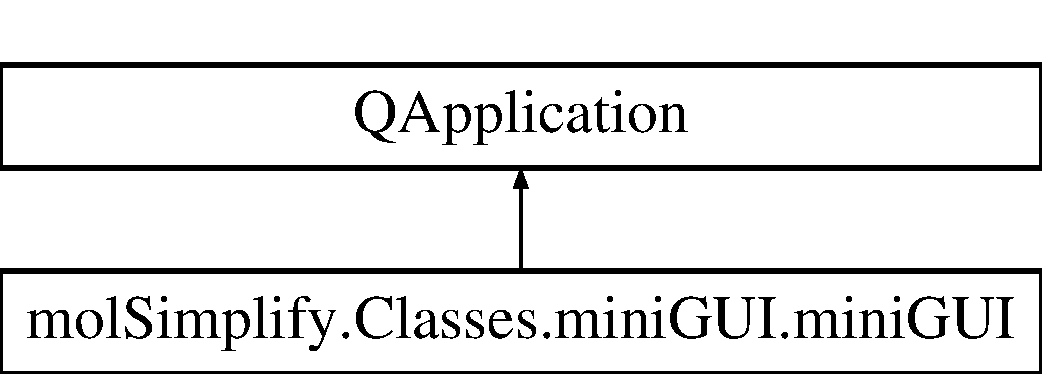
\includegraphics[height=2.000000cm]{classmolSimplify_1_1Classes_1_1miniGUI_1_1miniGUI}
\end{center}
\end{figure}
\subsection*{Public Member Functions}
\begin{DoxyCompactItemize}
\item 
def \hyperlink{classmolSimplify_1_1Classes_1_1miniGUI_1_1miniGUI_aad88ec5d3df2668211cbd2433356a848}{\+\_\+\+\_\+init\+\_\+\+\_\+} (self, args)
\item 
def \hyperlink{classmolSimplify_1_1Classes_1_1miniGUI_1_1miniGUI_a811c9618658a0ccf8ea05675a7548b95}{addsvg} (self, filename)
\item 
def \hyperlink{classmolSimplify_1_1Classes_1_1miniGUI_1_1miniGUI_a7b754f3a1031329ab7f45f6edf23a44f}{show} (self)
\end{DoxyCompactItemize}
\subsection*{Public Attributes}
\begin{DoxyCompactItemize}
\item 
\hyperlink{classmolSimplify_1_1Classes_1_1miniGUI_1_1miniGUI_ad87646506731f9daca029e19d7e77bc8}{window}
\item 
\hyperlink{classmolSimplify_1_1Classes_1_1miniGUI_1_1miniGUI_ab0e0287a99e55edfe42679806ffe4173}{lwindow}
\item 
\hyperlink{classmolSimplify_1_1Classes_1_1miniGUI_1_1miniGUI_a0af9c62718e1c849c23dc2256b1c70c3}{lgrid}
\item 
\hyperlink{classmolSimplify_1_1Classes_1_1miniGUI_1_1miniGUI_af9f9bd955f06b1cd712c4ec3083d7079}{svgwidget}
\end{DoxyCompactItemize}


\subsection{Detailed Description}
Mini G\+UI class for drawing molecules from the command line. 

\subsection{Constructor \& Destructor Documentation}
\mbox{\Hypertarget{classmolSimplify_1_1Classes_1_1miniGUI_1_1miniGUI_aad88ec5d3df2668211cbd2433356a848}\label{classmolSimplify_1_1Classes_1_1miniGUI_1_1miniGUI_aad88ec5d3df2668211cbd2433356a848}} 
\index{mol\+Simplify\+::\+Classes\+::mini\+G\+U\+I\+::mini\+G\+UI@{mol\+Simplify\+::\+Classes\+::mini\+G\+U\+I\+::mini\+G\+UI}!\+\_\+\+\_\+init\+\_\+\+\_\+@{\+\_\+\+\_\+init\+\_\+\+\_\+}}
\index{\+\_\+\+\_\+init\+\_\+\+\_\+@{\+\_\+\+\_\+init\+\_\+\+\_\+}!mol\+Simplify\+::\+Classes\+::mini\+G\+U\+I\+::mini\+G\+UI@{mol\+Simplify\+::\+Classes\+::mini\+G\+U\+I\+::mini\+G\+UI}}
\subsubsection{\texorpdfstring{\+\_\+\+\_\+init\+\_\+\+\_\+()}{\_\_init\_\_()}}
{\footnotesize\ttfamily def mol\+Simplify.\+Classes.\+mini\+G\+U\+I.\+mini\+G\+U\+I.\+\_\+\+\_\+init\+\_\+\+\_\+ (\begin{DoxyParamCaption}\item[{}]{self,  }\item[{}]{args }\end{DoxyParamCaption})}



\subsection{Member Function Documentation}
\mbox{\Hypertarget{classmolSimplify_1_1Classes_1_1miniGUI_1_1miniGUI_a811c9618658a0ccf8ea05675a7548b95}\label{classmolSimplify_1_1Classes_1_1miniGUI_1_1miniGUI_a811c9618658a0ccf8ea05675a7548b95}} 
\index{mol\+Simplify\+::\+Classes\+::mini\+G\+U\+I\+::mini\+G\+UI@{mol\+Simplify\+::\+Classes\+::mini\+G\+U\+I\+::mini\+G\+UI}!addsvg@{addsvg}}
\index{addsvg@{addsvg}!mol\+Simplify\+::\+Classes\+::mini\+G\+U\+I\+::mini\+G\+UI@{mol\+Simplify\+::\+Classes\+::mini\+G\+U\+I\+::mini\+G\+UI}}
\subsubsection{\texorpdfstring{addsvg()}{addsvg()}}
{\footnotesize\ttfamily def mol\+Simplify.\+Classes.\+mini\+G\+U\+I.\+mini\+G\+U\+I.\+addsvg (\begin{DoxyParamCaption}\item[{}]{self,  }\item[{}]{filename }\end{DoxyParamCaption})}

\mbox{\Hypertarget{classmolSimplify_1_1Classes_1_1miniGUI_1_1miniGUI_a7b754f3a1031329ab7f45f6edf23a44f}\label{classmolSimplify_1_1Classes_1_1miniGUI_1_1miniGUI_a7b754f3a1031329ab7f45f6edf23a44f}} 
\index{mol\+Simplify\+::\+Classes\+::mini\+G\+U\+I\+::mini\+G\+UI@{mol\+Simplify\+::\+Classes\+::mini\+G\+U\+I\+::mini\+G\+UI}!show@{show}}
\index{show@{show}!mol\+Simplify\+::\+Classes\+::mini\+G\+U\+I\+::mini\+G\+UI@{mol\+Simplify\+::\+Classes\+::mini\+G\+U\+I\+::mini\+G\+UI}}
\subsubsection{\texorpdfstring{show()}{show()}}
{\footnotesize\ttfamily def mol\+Simplify.\+Classes.\+mini\+G\+U\+I.\+mini\+G\+U\+I.\+show (\begin{DoxyParamCaption}\item[{}]{self }\end{DoxyParamCaption})}



\subsection{Member Data Documentation}
\mbox{\Hypertarget{classmolSimplify_1_1Classes_1_1miniGUI_1_1miniGUI_a0af9c62718e1c849c23dc2256b1c70c3}\label{classmolSimplify_1_1Classes_1_1miniGUI_1_1miniGUI_a0af9c62718e1c849c23dc2256b1c70c3}} 
\index{mol\+Simplify\+::\+Classes\+::mini\+G\+U\+I\+::mini\+G\+UI@{mol\+Simplify\+::\+Classes\+::mini\+G\+U\+I\+::mini\+G\+UI}!lgrid@{lgrid}}
\index{lgrid@{lgrid}!mol\+Simplify\+::\+Classes\+::mini\+G\+U\+I\+::mini\+G\+UI@{mol\+Simplify\+::\+Classes\+::mini\+G\+U\+I\+::mini\+G\+UI}}
\subsubsection{\texorpdfstring{lgrid}{lgrid}}
{\footnotesize\ttfamily mol\+Simplify.\+Classes.\+mini\+G\+U\+I.\+mini\+G\+U\+I.\+lgrid}

\mbox{\Hypertarget{classmolSimplify_1_1Classes_1_1miniGUI_1_1miniGUI_ab0e0287a99e55edfe42679806ffe4173}\label{classmolSimplify_1_1Classes_1_1miniGUI_1_1miniGUI_ab0e0287a99e55edfe42679806ffe4173}} 
\index{mol\+Simplify\+::\+Classes\+::mini\+G\+U\+I\+::mini\+G\+UI@{mol\+Simplify\+::\+Classes\+::mini\+G\+U\+I\+::mini\+G\+UI}!lwindow@{lwindow}}
\index{lwindow@{lwindow}!mol\+Simplify\+::\+Classes\+::mini\+G\+U\+I\+::mini\+G\+UI@{mol\+Simplify\+::\+Classes\+::mini\+G\+U\+I\+::mini\+G\+UI}}
\subsubsection{\texorpdfstring{lwindow}{lwindow}}
{\footnotesize\ttfamily mol\+Simplify.\+Classes.\+mini\+G\+U\+I.\+mini\+G\+U\+I.\+lwindow}

\mbox{\Hypertarget{classmolSimplify_1_1Classes_1_1miniGUI_1_1miniGUI_af9f9bd955f06b1cd712c4ec3083d7079}\label{classmolSimplify_1_1Classes_1_1miniGUI_1_1miniGUI_af9f9bd955f06b1cd712c4ec3083d7079}} 
\index{mol\+Simplify\+::\+Classes\+::mini\+G\+U\+I\+::mini\+G\+UI@{mol\+Simplify\+::\+Classes\+::mini\+G\+U\+I\+::mini\+G\+UI}!svgwidget@{svgwidget}}
\index{svgwidget@{svgwidget}!mol\+Simplify\+::\+Classes\+::mini\+G\+U\+I\+::mini\+G\+UI@{mol\+Simplify\+::\+Classes\+::mini\+G\+U\+I\+::mini\+G\+UI}}
\subsubsection{\texorpdfstring{svgwidget}{svgwidget}}
{\footnotesize\ttfamily mol\+Simplify.\+Classes.\+mini\+G\+U\+I.\+mini\+G\+U\+I.\+svgwidget}

\mbox{\Hypertarget{classmolSimplify_1_1Classes_1_1miniGUI_1_1miniGUI_ad87646506731f9daca029e19d7e77bc8}\label{classmolSimplify_1_1Classes_1_1miniGUI_1_1miniGUI_ad87646506731f9daca029e19d7e77bc8}} 
\index{mol\+Simplify\+::\+Classes\+::mini\+G\+U\+I\+::mini\+G\+UI@{mol\+Simplify\+::\+Classes\+::mini\+G\+U\+I\+::mini\+G\+UI}!window@{window}}
\index{window@{window}!mol\+Simplify\+::\+Classes\+::mini\+G\+U\+I\+::mini\+G\+UI@{mol\+Simplify\+::\+Classes\+::mini\+G\+U\+I\+::mini\+G\+UI}}
\subsubsection{\texorpdfstring{window}{window}}
{\footnotesize\ttfamily mol\+Simplify.\+Classes.\+mini\+G\+U\+I.\+mini\+G\+U\+I.\+window}



The documentation for this class was generated from the following file\+:\begin{DoxyCompactItemize}
\item 
Classes/\hyperlink{miniGUI_8py}{mini\+G\+U\+I.\+py}\end{DoxyCompactItemize}

\hypertarget{classmolSimplify_1_1Classes_1_1mol3D_1_1mol3D}{}\section{mol\+Simplify.\+Classes.\+mol3\+D.\+mol3D Class Reference}
\label{classmolSimplify_1_1Classes_1_1mol3D_1_1mol3D}\index{mol\+Simplify.\+Classes.\+mol3\+D.\+mol3D@{mol\+Simplify.\+Classes.\+mol3\+D.\+mol3D}}


Class for molecules that will be used to manipulate coordinates and other properties.  


\subsection*{Public Member Functions}
\begin{DoxyCompactItemize}
\item 
def \hyperlink{classmolSimplify_1_1Classes_1_1mol3D_1_1mol3D_ad12e0f1f0f180b0ed25d8d9aee9e7a82}{\+\_\+\+\_\+init\+\_\+\+\_\+} (self)
\begin{DoxyCompactList}\small\item\em Constructor. \end{DoxyCompactList}\item 
def \hyperlink{classmolSimplify_1_1Classes_1_1mol3D_1_1mol3D_a444e22d04c8ec79f1b2ce77ee9e1e8fc}{add\+Atom} (self, atom)
\begin{DoxyCompactList}\small\item\em Add atom to molecule. \end{DoxyCompactList}\item 
def \hyperlink{classmolSimplify_1_1Classes_1_1mol3D_1_1mol3D_ab1d82358efa2110c56e1caf3ba9433e5}{alignmol} (self, atom1, atom2)
\begin{DoxyCompactList}\small\item\em Aligns two molecules such that the coordinates of two atoms overlap. \end{DoxyCompactList}\item 
def \hyperlink{classmolSimplify_1_1Classes_1_1mol3D_1_1mol3D_aa37a3e5878925148c6b6e38f6a6cf59c}{B\+CM} (self, idx1, idx2, d)
\begin{DoxyCompactList}\small\item\em Performs bond centric manipulation (same as Avogadro, stretching/squeezing bonds) \end{DoxyCompactList}\item 
def \hyperlink{classmolSimplify_1_1Classes_1_1mol3D_1_1mol3D_ac2341892da1c1333802cda42da7cca3e}{centermass} (self)
\begin{DoxyCompactList}\small\item\em Computes coordinates of center of mass of molecule. \end{DoxyCompactList}\item 
def \hyperlink{classmolSimplify_1_1Classes_1_1mol3D_1_1mol3D_a0e4c145ac4c16e7be70cec1a3e03f6b7}{centersym} (self)
\begin{DoxyCompactList}\small\item\em Computes coordinates of center of symmetry of molecule. \end{DoxyCompactList}\item 
def \hyperlink{classmolSimplify_1_1Classes_1_1mol3D_1_1mol3D_a10ce42207cd8291c685640438f8de1a8}{convert2mol3D} (self)
\begin{DoxyCompactList}\small\item\em Converts O\+B\+Mol to \hyperlink{classmolSimplify_1_1Classes_1_1mol3D_1_1mol3D}{mol3D}. \end{DoxyCompactList}\item 
def \hyperlink{classmolSimplify_1_1Classes_1_1mol3D_1_1mol3D_acc86e8896c87c6287cfe504321ec8b11}{convert2\+O\+B\+Mol} (self)
\begin{DoxyCompactList}\small\item\em Converts \hyperlink{classmolSimplify_1_1Classes_1_1mol3D_1_1mol3D}{mol3D} to O\+B\+Mol. \end{DoxyCompactList}\item 
def \hyperlink{classmolSimplify_1_1Classes_1_1mol3D_1_1mol3D_a8c96247d4d06ac9d1b241af45e79d94a}{combine} (self, mol)
\begin{DoxyCompactList}\small\item\em Combines two molecules. \end{DoxyCompactList}\item 
def \hyperlink{classmolSimplify_1_1Classes_1_1mol3D_1_1mol3D_a551393e5c2417086b3b7855be3cf5957}{coords} (self)
\begin{DoxyCompactList}\small\item\em Prints coordinates of all atoms in molecule. \end{DoxyCompactList}\item 
def \hyperlink{classmolSimplify_1_1Classes_1_1mol3D_1_1mol3D_a305748724bd9be10c324302f046e3815}{coordsvect} (self)
\begin{DoxyCompactList}\small\item\em Returns coordinates of all atoms in molecule as a list of lists. \end{DoxyCompactList}\item 
def \hyperlink{classmolSimplify_1_1Classes_1_1mol3D_1_1mol3D_a09b722d1243e562169a88a591812a2ed}{copymol3D} (self, mol0)
\begin{DoxyCompactList}\small\item\em Copies properties and atoms of another existing \hyperlink{classmolSimplify_1_1Classes_1_1mol3D_1_1mol3D}{mol3D} object into current \hyperlink{classmolSimplify_1_1Classes_1_1mol3D_1_1mol3D}{mol3D} object. \end{DoxyCompactList}\item 
def \hyperlink{classmolSimplify_1_1Classes_1_1mol3D_1_1mol3D_afa77b09b79aeb68ed3b50b51987c61dc}{create\+Molecular\+Graph} (self)
\begin{DoxyCompactList}\small\item\em Create molecular graph (connectivity matrix) from \hyperlink{classmolSimplify_1_1Classes_1_1mol3D_1_1mol3D}{mol3D} info. \end{DoxyCompactList}\item 
def \hyperlink{classmolSimplify_1_1Classes_1_1mol3D_1_1mol3D_a6838664445a9896c703e0ffe2542ceef}{deleteatom} (self, atom\+Idx)
\begin{DoxyCompactList}\small\item\em Deletes specific atom from molecule. \end{DoxyCompactList}\item 
def \hyperlink{classmolSimplify_1_1Classes_1_1mol3D_1_1mol3D_a3d0541772724aa1a54e8cb6c8de77ea7}{freezeatom} (self, atom\+Idx)
\begin{DoxyCompactList}\small\item\em Freezes specific atom in molecule. \end{DoxyCompactList}\item 
def \hyperlink{classmolSimplify_1_1Classes_1_1mol3D_1_1mol3D_a98613e0d849dd341b6cec837877e214b}{deleteatoms} (self, Alist)
\begin{DoxyCompactList}\small\item\em Deletes list of atoms from molecule. \end{DoxyCompactList}\item 
def \hyperlink{classmolSimplify_1_1Classes_1_1mol3D_1_1mol3D_a629f2ff84af7df7a809fe5e8f879f6a3}{freezeatoms} (self, Alist)
\begin{DoxyCompactList}\small\item\em Freezes list of atoms in molecule. \end{DoxyCompactList}\item 
def \hyperlink{classmolSimplify_1_1Classes_1_1mol3D_1_1mol3D_a91e56cc05405772f174a4eda98d86f41}{delete\+Hs} (self)
\begin{DoxyCompactList}\small\item\em Deletes all hydrogens from molecule. \end{DoxyCompactList}\item 
def \hyperlink{classmolSimplify_1_1Classes_1_1mol3D_1_1mol3D_a7f5c446c9d071037c5500408ab57a8f6}{distance} (self, mol)
\begin{DoxyCompactList}\small\item\em Gets distance between centers of mass of two molecules. \end{DoxyCompactList}\item 
def \hyperlink{classmolSimplify_1_1Classes_1_1mol3D_1_1mol3D_afc2743674602def7c8d9457cb40a2899}{draw\+\_\+svg} (self, filename)
\begin{DoxyCompactList}\small\item\em Creates and saves an svg file of the molecule. \end{DoxyCompactList}\item 
def \hyperlink{classmolSimplify_1_1Classes_1_1mol3D_1_1mol3D_a3a4f5d88b74124789e380f28d1038fad}{findclose\+Metal} (self, atom0)
\begin{DoxyCompactList}\small\item\em Finds closest metal atom to a given atom. \end{DoxyCompactList}\item 
def \hyperlink{classmolSimplify_1_1Classes_1_1mol3D_1_1mol3D_aff49b31bdc2ef9d33a3b67642b6f70d2}{find\+Metal} (self)
\begin{DoxyCompactList}\small\item\em Finds metal atoms in molecule. \end{DoxyCompactList}\item 
def \hyperlink{classmolSimplify_1_1Classes_1_1mol3D_1_1mol3D_adb95387b07a9714c03db4975a192e08c}{find\+Atomsby\+Symbol} (self, sym)
\begin{DoxyCompactList}\small\item\em Finds atoms in molecule with given symbol. \end{DoxyCompactList}\item 
def \hyperlink{classmolSimplify_1_1Classes_1_1mol3D_1_1mol3D_a0b5cecd561856f3b3a7525ce75bc5282}{findsub\+Mol} (self, atom0, atomN)
\begin{DoxyCompactList}\small\item\em Finds a submolecule within the molecule given the starting atom and the separating atom. \end{DoxyCompactList}\item 
def \hyperlink{classmolSimplify_1_1Classes_1_1mol3D_1_1mol3D_ad30b31562cb3c57c2758554ff7e3714d}{get\+Atom} (self, idx)
\begin{DoxyCompactList}\small\item\em Gets an atom with specified index. \end{DoxyCompactList}\item 
def \hyperlink{classmolSimplify_1_1Classes_1_1mol3D_1_1mol3D_a28a0a4e056758a2cc390899e9b34baaa}{get\+Atoms} (self)
\begin{DoxyCompactList}\small\item\em Gets atoms in molecule. \end{DoxyCompactList}\item 
def \hyperlink{classmolSimplify_1_1Classes_1_1mol3D_1_1mol3D_a53c044279fd5d0dace4f220c950921fa}{get\+Atom\+Types} (self)
\begin{DoxyCompactList}\small\item\em Gets number of unique elements in molecule. \end{DoxyCompactList}\item 
def \hyperlink{classmolSimplify_1_1Classes_1_1mol3D_1_1mol3D_a67307accd49f78a076a0139591fdefb7}{get\+Atom\+Coords} (self, idx)
\begin{DoxyCompactList}\small\item\em Gets coordinates of atom with specified index. \end{DoxyCompactList}\item 
def \hyperlink{classmolSimplify_1_1Classes_1_1mol3D_1_1mol3D_a394c680ec3eddbcc22ebcec76d211218}{get\+Bonded\+Atoms} (self, ind)
\begin{DoxyCompactList}\small\item\em Gets atoms bonded to a specific atom. \end{DoxyCompactList}\item 
def \hyperlink{classmolSimplify_1_1Classes_1_1mol3D_1_1mol3D_a054076c86f015de56353017cc391ba4c}{get\+Bonded\+Atoms\+Oct} (self, ind, CN=6, debug=False)
\begin{DoxyCompactList}\small\item\em Gets atoms bonded to a specific atom specialized for octahedral complexes. \end{DoxyCompactList}\item 
def \hyperlink{classmolSimplify_1_1Classes_1_1mol3D_1_1mol3D_afa8b020ddc30de3b82be2568be20aaa5}{get\+Bonded\+Atoms\+Smart} (self, ind)
\begin{DoxyCompactList}\small\item\em Gets atoms bonded to a specific atom using the molecular graph, or creates it. \end{DoxyCompactList}\item 
def \hyperlink{classmolSimplify_1_1Classes_1_1mol3D_1_1mol3D_acda82e48cde5996f32a55e0acbdf052e}{get\+Bonded\+AtomsnotH} (self, ind)
\begin{DoxyCompactList}\small\item\em Gets non-\/H atoms bonded to a specific atom. \end{DoxyCompactList}\item 
def \hyperlink{classmolSimplify_1_1Classes_1_1mol3D_1_1mol3D_ae4d631214022274b00b853768706d55a}{getfar\+Atomdir} (self, uP)
\begin{DoxyCompactList}\small\item\em Gets atom that is furthest from the molecule C\+OM along a given direction and returns the corresponding distance. \end{DoxyCompactList}\item 
def \hyperlink{classmolSimplify_1_1Classes_1_1mol3D_1_1mol3D_a5b27778bb5e730b3911e0fe9192a4c0e}{get\+Hs} (self)
\begin{DoxyCompactList}\small\item\em Gets H atoms in molecule. \end{DoxyCompactList}\item 
def \hyperlink{classmolSimplify_1_1Classes_1_1mol3D_1_1mol3D_a232adbbe11745aac4561a15fe1850df4}{get\+Hsby\+Atom} (self, ratom)
\begin{DoxyCompactList}\small\item\em Gets H atoms bonded to specific \hyperlink{namespacemolSimplify_1_1Classes_1_1atom3D}{atom3D} in molecule. \end{DoxyCompactList}\item 
def \hyperlink{classmolSimplify_1_1Classes_1_1mol3D_1_1mol3D_a99730d5cf790e512a55fbe0d1fd863c7}{get\+Hsby\+Index} (self, idx)
\begin{DoxyCompactList}\small\item\em Gets H atoms bonded to specific atom index in molecule. \end{DoxyCompactList}\item 
def \hyperlink{classmolSimplify_1_1Classes_1_1mol3D_1_1mol3D_a6f4f405d4a3d80e9810a73a199662800}{get\+Closest\+Atom} (self, atom0)
\begin{DoxyCompactList}\small\item\em Gets index of closest atom to reference atom. \end{DoxyCompactList}\item 
def \hyperlink{classmolSimplify_1_1Classes_1_1mol3D_1_1mol3D_aae3d38b16c8876fd11e6a170b3e18df0}{get\+Mask} (self, mask)
\begin{DoxyCompactList}\small\item\em Gets point that corresponds to mask. \end{DoxyCompactList}\item 
def \hyperlink{classmolSimplify_1_1Classes_1_1mol3D_1_1mol3D_a3f137b174fb3b427893ed88d685888ce}{get\+Closest\+Atomno\+Hs} (self, atom0)
\begin{DoxyCompactList}\small\item\em Gets index of closest non-\/H atom to another atom. \end{DoxyCompactList}\item 
def \hyperlink{classmolSimplify_1_1Classes_1_1mol3D_1_1mol3D_abdd4f09ed5f39c96a5025fa9d049f2e8}{get\+Dist\+To\+Metal} (self, idx, metalx)
\begin{DoxyCompactList}\small\item\em Gets distance between two atoms in molecule. \end{DoxyCompactList}\item 
def \hyperlink{classmolSimplify_1_1Classes_1_1mol3D_1_1mol3D_a911ffafa9384284b123be8c1670220ca}{get\+Closest\+Atomno\+Hs2} (self, atidx)
\begin{DoxyCompactList}\small\item\em Gets index of closest non-\/H atom to another atom. \end{DoxyCompactList}\item 
def \hyperlink{classmolSimplify_1_1Classes_1_1mol3D_1_1mol3D_a4a723fdb1daadc53a524243198fb15cb}{get\+O\+B\+Mol} (self, fst, convtype, ffclean=False)
\begin{DoxyCompactList}\small\item\em Initializes O\+B\+Mol object from a file or S\+M\+I\+L\+ES string. \end{DoxyCompactList}\item 
def \hyperlink{classmolSimplify_1_1Classes_1_1mol3D_1_1mol3D_ab2935f2310ca23b0c77e4ef3ac11a6f9}{initialize} (self)
\begin{DoxyCompactList}\small\item\em Removes attributes from \hyperlink{classmolSimplify_1_1Classes_1_1mol3D_1_1mol3D}{mol3D} object. \end{DoxyCompactList}\item 
def \hyperlink{classmolSimplify_1_1Classes_1_1mol3D_1_1mol3D_a7d3399262fb568aeec589f86ff59d376}{maxdist} (self, mol)
\begin{DoxyCompactList}\small\item\em Calculates the largest distance between atoms of two molecules. \end{DoxyCompactList}\item 
def \hyperlink{classmolSimplify_1_1Classes_1_1mol3D_1_1mol3D_ab051fea5908eab8ddcd39d4ea4688657}{mindist} (self, mol)
\begin{DoxyCompactList}\small\item\em Calculates the smallest distance between atoms of two molecules. \end{DoxyCompactList}\item 
def \hyperlink{classmolSimplify_1_1Classes_1_1mol3D_1_1mol3D_abc383cd8e5f7a2963b5b220fe5f23c02}{mindistmol} (self)
\begin{DoxyCompactList}\small\item\em Calculates the smallest distance between atoms in the molecule. \end{DoxyCompactList}\item 
def \hyperlink{classmolSimplify_1_1Classes_1_1mol3D_1_1mol3D_a9002b30e6f3e13fb41c0080f4fec6ce1}{mindisttopoint} (self, point)
\begin{DoxyCompactList}\small\item\em Calculates the smallest distance from atoms in the molecule to a given point. \end{DoxyCompactList}\item 
def \hyperlink{classmolSimplify_1_1Classes_1_1mol3D_1_1mol3D_a613d343492efdeda0c47700654157b3d}{mindistnonH} (self, mol)
\begin{DoxyCompactList}\small\item\em Calculates the smallest distance between non-\/H atoms of two molecules. \end{DoxyCompactList}\item 
def \hyperlink{classmolSimplify_1_1Classes_1_1mol3D_1_1mol3D_aec0cabe05c899a3825c523add5e352ce}{molsize} (self)
\begin{DoxyCompactList}\small\item\em Calculates the size of the molecule, as quantified by the max. \end{DoxyCompactList}\item 
def \hyperlink{classmolSimplify_1_1Classes_1_1mol3D_1_1mol3D_aab1e703e70f941dfc764a47dfdd6a121}{overlapcheck} (self, mol, silence)
\begin{DoxyCompactList}\small\item\em Checks for overlap with another molecule. \end{DoxyCompactList}\item 
def \hyperlink{classmolSimplify_1_1Classes_1_1mol3D_1_1mol3D_a52aafa6742ea7f501a30b286bedfc4f4}{overlapcheckh} (self, mol)
\begin{DoxyCompactList}\small\item\em Checks for overlap with another molecule with increased tolerance. \end{DoxyCompactList}\item 
def \hyperlink{classmolSimplify_1_1Classes_1_1mol3D_1_1mol3D_ae6f619f46f387b2b609807fe06a6876a}{printxyz} (self)
\begin{DoxyCompactList}\small\item\em Prints xyz coordinates to stdout. \end{DoxyCompactList}\item 
def \hyperlink{classmolSimplify_1_1Classes_1_1mol3D_1_1mol3D_a693d0fb9d44650a500c91cac47e93a80}{readfromxyz} (self, filename)
\begin{DoxyCompactList}\small\item\em Load molecule from xyz file. \end{DoxyCompactList}\item 
def \hyperlink{classmolSimplify_1_1Classes_1_1mol3D_1_1mol3D_a970c3cdf7b4a051715a89e284d4227e6}{rmsd} (self, mol2)
\begin{DoxyCompactList}\small\item\em Computes R\+M\+SD between two molecules. \end{DoxyCompactList}\item 
def \hyperlink{classmolSimplify_1_1Classes_1_1mol3D_1_1mol3D_af79c7b686fca67c122bb1e0507f845a6}{sanitycheck} (self, silence)
\begin{DoxyCompactList}\small\item\em Checks for overlap within the molecule. \end{DoxyCompactList}\item 
def \hyperlink{classmolSimplify_1_1Classes_1_1mol3D_1_1mol3D_a27bd691cb90ab44c3acc746dc637baed}{translate} (self, dxyz)
\begin{DoxyCompactList}\small\item\em Translate all atoms by given vector. \end{DoxyCompactList}\item 
def \hyperlink{classmolSimplify_1_1Classes_1_1mol3D_1_1mol3D_a773c0ca887457100e8034a8eacc28103}{writegxyz} (self, filename)
\begin{DoxyCompactList}\small\item\em Writes xyz file in G\+A\+M\+E\+SS format. \end{DoxyCompactList}\item 
def \hyperlink{classmolSimplify_1_1Classes_1_1mol3D_1_1mol3D_a9d338e17fae1e6f4d7a9012a76844e7c}{writexyz} (self, filename)
\begin{DoxyCompactList}\small\item\em Writes xyz file. \end{DoxyCompactList}\item 
def \hyperlink{classmolSimplify_1_1Classes_1_1mol3D_1_1mol3D_a21f8c2e9da6a3f0ec19120c00700f32b}{writemxyz} (self, mol, filename)
\begin{DoxyCompactList}\small\item\em Writes xyz file for 2 molecules combined. \end{DoxyCompactList}\item 
def \hyperlink{classmolSimplify_1_1Classes_1_1mol3D_1_1mol3D_a7448ad5d35a2801d08a05c3b5eea4835}{writesepxyz} (self, mol, filename)
\begin{DoxyCompactList}\small\item\em Writes xyz file for 2 molecules separated. \end{DoxyCompactList}\item 
def \hyperlink{classmolSimplify_1_1Classes_1_1mol3D_1_1mol3D_ac5a779ac0e20d07b60dc30fdb9a0f4d1}{\+\_\+\+\_\+repr\+\_\+\+\_\+} (self)
\begin{DoxyCompactList}\small\item\em Print methods. \end{DoxyCompactList}\end{DoxyCompactItemize}
\subsection*{Public Attributes}
\begin{DoxyCompactItemize}
\item 
\hyperlink{classmolSimplify_1_1Classes_1_1mol3D_1_1mol3D_af02359e712403cf94bda038aeadbaa58}{atoms}
\begin{DoxyCompactList}\small\item\em List of \hyperlink{namespacemolSimplify_1_1Classes_1_1atom3D}{atom3D} objects. \end{DoxyCompactList}\item 
\hyperlink{classmolSimplify_1_1Classes_1_1mol3D_1_1mol3D_af232ea2794ec4a1968befbad30d48913}{natoms}
\begin{DoxyCompactList}\small\item\em Number of atoms. \end{DoxyCompactList}\item 
\hyperlink{classmolSimplify_1_1Classes_1_1mol3D_1_1mol3D_abd8025bde323e199207f372539fc0ceb}{mass}
\begin{DoxyCompactList}\small\item\em Mass of molecule. \end{DoxyCompactList}\item 
\hyperlink{classmolSimplify_1_1Classes_1_1mol3D_1_1mol3D_a8ea7381eb4e01c2b290446c7299dad9a}{size}
\begin{DoxyCompactList}\small\item\em Size of molecule. \end{DoxyCompactList}\item 
\hyperlink{classmolSimplify_1_1Classes_1_1mol3D_1_1mol3D_aa81f118b37cdb2b11681f1361b51fed7}{charge}
\begin{DoxyCompactList}\small\item\em Charge of molecule. \end{DoxyCompactList}\item 
\hyperlink{classmolSimplify_1_1Classes_1_1mol3D_1_1mol3D_ac8526f460332be176e5009f6e2ae8745}{ffopt}
\begin{DoxyCompactList}\small\item\em Force field optimization settings. \end{DoxyCompactList}\item 
\hyperlink{classmolSimplify_1_1Classes_1_1mol3D_1_1mol3D_a06cc059cb532fb64b3e9faa84ae1f8c9}{name}
\begin{DoxyCompactList}\small\item\em Name of molecule. \end{DoxyCompactList}\item 
\hyperlink{classmolSimplify_1_1Classes_1_1mol3D_1_1mol3D_ac6f2ce6966f1126c52b32f0aa40612a4}{O\+B\+Mol}
\begin{DoxyCompactList}\small\item\em Holder for openbabel molecule. \end{DoxyCompactList}\item 
\hyperlink{classmolSimplify_1_1Classes_1_1mol3D_1_1mol3D_a7cec79699a619b85d5e23e869327749b}{cat}
\begin{DoxyCompactList}\small\item\em List of connection atoms. \end{DoxyCompactList}\item 
\hyperlink{classmolSimplify_1_1Classes_1_1mol3D_1_1mol3D_a5bdeed75bc96b42a06b2ea277b431739}{denticity}
\begin{DoxyCompactList}\small\item\em Denticity. \end{DoxyCompactList}\item 
\hyperlink{classmolSimplify_1_1Classes_1_1mol3D_1_1mol3D_a606148a9c1137fcad6528b1e5c34a5c4}{ident}
\begin{DoxyCompactList}\small\item\em Identifier. \end{DoxyCompactList}\item 
\hyperlink{classmolSimplify_1_1Classes_1_1mol3D_1_1mol3D_a6f203eafd5348c5bd650356edda9b84a}{globs}
\begin{DoxyCompactList}\small\item\em Holder for global variables. \end{DoxyCompactList}\item 
\hyperlink{classmolSimplify_1_1Classes_1_1mol3D_1_1mol3D_aa14392db397618bd85a06f44f43360a2}{graph}
\begin{DoxyCompactList}\small\item\em Holder for molecular graph. \end{DoxyCompactList}\end{DoxyCompactItemize}


\subsection{Detailed Description}
Class for molecules that will be used to manipulate coordinates and other properties. 

\subsection{Constructor \& Destructor Documentation}
\mbox{\Hypertarget{classmolSimplify_1_1Classes_1_1mol3D_1_1mol3D_ad12e0f1f0f180b0ed25d8d9aee9e7a82}\label{classmolSimplify_1_1Classes_1_1mol3D_1_1mol3D_ad12e0f1f0f180b0ed25d8d9aee9e7a82}} 
\index{mol\+Simplify\+::\+Classes\+::mol3\+D\+::mol3D@{mol\+Simplify\+::\+Classes\+::mol3\+D\+::mol3D}!\+\_\+\+\_\+init\+\_\+\+\_\+@{\+\_\+\+\_\+init\+\_\+\+\_\+}}
\index{\+\_\+\+\_\+init\+\_\+\+\_\+@{\+\_\+\+\_\+init\+\_\+\+\_\+}!mol\+Simplify\+::\+Classes\+::mol3\+D\+::mol3D@{mol\+Simplify\+::\+Classes\+::mol3\+D\+::mol3D}}
\subsubsection{\texorpdfstring{\+\_\+\+\_\+init\+\_\+\+\_\+()}{\_\_init\_\_()}}
{\footnotesize\ttfamily def mol\+Simplify.\+Classes.\+mol3\+D.\+mol3\+D.\+\_\+\+\_\+init\+\_\+\+\_\+ (\begin{DoxyParamCaption}\item[{}]{self }\end{DoxyParamCaption})}



Constructor. 


\begin{DoxyParams}{Parameters}
{\em self} & The object pointer \\
\hline
\end{DoxyParams}


\subsection{Member Function Documentation}
\mbox{\Hypertarget{classmolSimplify_1_1Classes_1_1mol3D_1_1mol3D_ac5a779ac0e20d07b60dc30fdb9a0f4d1}\label{classmolSimplify_1_1Classes_1_1mol3D_1_1mol3D_ac5a779ac0e20d07b60dc30fdb9a0f4d1}} 
\index{mol\+Simplify\+::\+Classes\+::mol3\+D\+::mol3D@{mol\+Simplify\+::\+Classes\+::mol3\+D\+::mol3D}!\+\_\+\+\_\+repr\+\_\+\+\_\+@{\+\_\+\+\_\+repr\+\_\+\+\_\+}}
\index{\+\_\+\+\_\+repr\+\_\+\+\_\+@{\+\_\+\+\_\+repr\+\_\+\+\_\+}!mol\+Simplify\+::\+Classes\+::mol3\+D\+::mol3D@{mol\+Simplify\+::\+Classes\+::mol3\+D\+::mol3D}}
\subsubsection{\texorpdfstring{\+\_\+\+\_\+repr\+\_\+\+\_\+()}{\_\_repr\_\_()}}
{\footnotesize\ttfamily def mol\+Simplify.\+Classes.\+mol3\+D.\+mol3\+D.\+\_\+\+\_\+repr\+\_\+\+\_\+ (\begin{DoxyParamCaption}\item[{}]{self }\end{DoxyParamCaption})}



Print methods. 


\begin{DoxyParams}{Parameters}
{\em self} & The object pointer \\
\hline
\end{DoxyParams}
\begin{DoxyReturn}{Returns}
String with methods \begin{DoxyVerb}when calls mol3D object without attribute e.g. t \end{DoxyVerb}
 
\end{DoxyReturn}
\mbox{\Hypertarget{classmolSimplify_1_1Classes_1_1mol3D_1_1mol3D_a444e22d04c8ec79f1b2ce77ee9e1e8fc}\label{classmolSimplify_1_1Classes_1_1mol3D_1_1mol3D_a444e22d04c8ec79f1b2ce77ee9e1e8fc}} 
\index{mol\+Simplify\+::\+Classes\+::mol3\+D\+::mol3D@{mol\+Simplify\+::\+Classes\+::mol3\+D\+::mol3D}!add\+Atom@{add\+Atom}}
\index{add\+Atom@{add\+Atom}!mol\+Simplify\+::\+Classes\+::mol3\+D\+::mol3D@{mol\+Simplify\+::\+Classes\+::mol3\+D\+::mol3D}}
\subsubsection{\texorpdfstring{add\+Atom()}{addAtom()}}
{\footnotesize\ttfamily def mol\+Simplify.\+Classes.\+mol3\+D.\+mol3\+D.\+add\+Atom (\begin{DoxyParamCaption}\item[{}]{self,  }\item[{}]{atom }\end{DoxyParamCaption})}



Add atom to molecule. 

Added atom is appended to the end of the list. 
\begin{DoxyParams}{Parameters}
{\em self} & The object pointer \\
\hline
{\em atom} & \hyperlink{namespacemolSimplify_1_1Classes_1_1atom3D}{atom3D} of atom to be added \\
\hline
\end{DoxyParams}
\mbox{\Hypertarget{classmolSimplify_1_1Classes_1_1mol3D_1_1mol3D_ab1d82358efa2110c56e1caf3ba9433e5}\label{classmolSimplify_1_1Classes_1_1mol3D_1_1mol3D_ab1d82358efa2110c56e1caf3ba9433e5}} 
\index{mol\+Simplify\+::\+Classes\+::mol3\+D\+::mol3D@{mol\+Simplify\+::\+Classes\+::mol3\+D\+::mol3D}!alignmol@{alignmol}}
\index{alignmol@{alignmol}!mol\+Simplify\+::\+Classes\+::mol3\+D\+::mol3D@{mol\+Simplify\+::\+Classes\+::mol3\+D\+::mol3D}}
\subsubsection{\texorpdfstring{alignmol()}{alignmol()}}
{\footnotesize\ttfamily def mol\+Simplify.\+Classes.\+mol3\+D.\+mol3\+D.\+alignmol (\begin{DoxyParamCaption}\item[{}]{self,  }\item[{}]{atom1,  }\item[{}]{atom2 }\end{DoxyParamCaption})}



Aligns two molecules such that the coordinates of two atoms overlap. 

Second molecules is translated relative to the first. No rotations are performed here. Use other functions for rotations. 
\begin{DoxyParams}{Parameters}
{\em self} & The object pointer \\
\hline
{\em atom1} & \hyperlink{namespacemolSimplify_1_1Classes_1_1atom3D}{atom3D} of reference atom in first molecule (not translated) \\
\hline
{\em atom2} & \hyperlink{namespacemolSimplify_1_1Classes_1_1atom3D}{atom3D} of reference atom in second molecule (translated) \\
\hline
\end{DoxyParams}
\mbox{\Hypertarget{classmolSimplify_1_1Classes_1_1mol3D_1_1mol3D_aa37a3e5878925148c6b6e38f6a6cf59c}\label{classmolSimplify_1_1Classes_1_1mol3D_1_1mol3D_aa37a3e5878925148c6b6e38f6a6cf59c}} 
\index{mol\+Simplify\+::\+Classes\+::mol3\+D\+::mol3D@{mol\+Simplify\+::\+Classes\+::mol3\+D\+::mol3D}!B\+CM@{B\+CM}}
\index{B\+CM@{B\+CM}!mol\+Simplify\+::\+Classes\+::mol3\+D\+::mol3D@{mol\+Simplify\+::\+Classes\+::mol3\+D\+::mol3D}}
\subsubsection{\texorpdfstring{B\+C\+M()}{BCM()}}
{\footnotesize\ttfamily def mol\+Simplify.\+Classes.\+mol3\+D.\+mol3\+D.\+B\+CM (\begin{DoxyParamCaption}\item[{}]{self,  }\item[{}]{idx1,  }\item[{}]{idx2,  }\item[{}]{d }\end{DoxyParamCaption})}



Performs bond centric manipulation (same as Avogadro, stretching/squeezing bonds) 

A submolecule is translated along the bond axis connecting it to an anchor atom.

Illustration\+: H3\+A-\/\+B\+H3 -\/$>$ H3\+A-\/---B\+H3 where B = idx1 and A = idx2 
\begin{DoxyParams}{Parameters}
{\em self} & The object pointer \\
\hline
{\em idx1} & Index of bonded atom containing submolecule to be moved \\
\hline
{\em idx2} & Index of anchor atom \\
\hline
{\em d} & New bond length in Angstroms \\
\hline
\end{DoxyParams}
\mbox{\Hypertarget{classmolSimplify_1_1Classes_1_1mol3D_1_1mol3D_ac2341892da1c1333802cda42da7cca3e}\label{classmolSimplify_1_1Classes_1_1mol3D_1_1mol3D_ac2341892da1c1333802cda42da7cca3e}} 
\index{mol\+Simplify\+::\+Classes\+::mol3\+D\+::mol3D@{mol\+Simplify\+::\+Classes\+::mol3\+D\+::mol3D}!centermass@{centermass}}
\index{centermass@{centermass}!mol\+Simplify\+::\+Classes\+::mol3\+D\+::mol3D@{mol\+Simplify\+::\+Classes\+::mol3\+D\+::mol3D}}
\subsubsection{\texorpdfstring{centermass()}{centermass()}}
{\footnotesize\ttfamily def mol\+Simplify.\+Classes.\+mol3\+D.\+mol3\+D.\+centermass (\begin{DoxyParamCaption}\item[{}]{self }\end{DoxyParamCaption})}



Computes coordinates of center of mass of molecule. 


\begin{DoxyParams}{Parameters}
{\em self} & The object pointer \\
\hline
\end{DoxyParams}
\begin{DoxyReturn}{Returns}
List of center of mass coordinates 
\end{DoxyReturn}
\mbox{\Hypertarget{classmolSimplify_1_1Classes_1_1mol3D_1_1mol3D_a0e4c145ac4c16e7be70cec1a3e03f6b7}\label{classmolSimplify_1_1Classes_1_1mol3D_1_1mol3D_a0e4c145ac4c16e7be70cec1a3e03f6b7}} 
\index{mol\+Simplify\+::\+Classes\+::mol3\+D\+::mol3D@{mol\+Simplify\+::\+Classes\+::mol3\+D\+::mol3D}!centersym@{centersym}}
\index{centersym@{centersym}!mol\+Simplify\+::\+Classes\+::mol3\+D\+::mol3D@{mol\+Simplify\+::\+Classes\+::mol3\+D\+::mol3D}}
\subsubsection{\texorpdfstring{centersym()}{centersym()}}
{\footnotesize\ttfamily def mol\+Simplify.\+Classes.\+mol3\+D.\+mol3\+D.\+centersym (\begin{DoxyParamCaption}\item[{}]{self }\end{DoxyParamCaption})}



Computes coordinates of center of symmetry of molecule. 

Identical to centermass, but not weighted by atomic masses. 
\begin{DoxyParams}{Parameters}
{\em self} & The object pointer \\
\hline
\end{DoxyParams}
\begin{DoxyReturn}{Returns}
List of center of symmetry coordinates 
\end{DoxyReturn}
\mbox{\Hypertarget{classmolSimplify_1_1Classes_1_1mol3D_1_1mol3D_a8c96247d4d06ac9d1b241af45e79d94a}\label{classmolSimplify_1_1Classes_1_1mol3D_1_1mol3D_a8c96247d4d06ac9d1b241af45e79d94a}} 
\index{mol\+Simplify\+::\+Classes\+::mol3\+D\+::mol3D@{mol\+Simplify\+::\+Classes\+::mol3\+D\+::mol3D}!combine@{combine}}
\index{combine@{combine}!mol\+Simplify\+::\+Classes\+::mol3\+D\+::mol3D@{mol\+Simplify\+::\+Classes\+::mol3\+D\+::mol3D}}
\subsubsection{\texorpdfstring{combine()}{combine()}}
{\footnotesize\ttfamily def mol\+Simplify.\+Classes.\+mol3\+D.\+mol3\+D.\+combine (\begin{DoxyParamCaption}\item[{}]{self,  }\item[{}]{mol }\end{DoxyParamCaption})}



Combines two molecules. 

Each atom in the second molecule is appended to the first while preserving orders. 
\begin{DoxyParams}{Parameters}
{\em self} & The object pointer \\
\hline
{\em mol} & \hyperlink{classmolSimplify_1_1Classes_1_1mol3D_1_1mol3D}{mol3D} containing molecule to be added \\
\hline
\end{DoxyParams}
\begin{DoxyReturn}{Returns}
\hyperlink{classmolSimplify_1_1Classes_1_1mol3D_1_1mol3D}{mol3D} contaning combined molecule 
\end{DoxyReturn}
\mbox{\Hypertarget{classmolSimplify_1_1Classes_1_1mol3D_1_1mol3D_a10ce42207cd8291c685640438f8de1a8}\label{classmolSimplify_1_1Classes_1_1mol3D_1_1mol3D_a10ce42207cd8291c685640438f8de1a8}} 
\index{mol\+Simplify\+::\+Classes\+::mol3\+D\+::mol3D@{mol\+Simplify\+::\+Classes\+::mol3\+D\+::mol3D}!convert2mol3D@{convert2mol3D}}
\index{convert2mol3D@{convert2mol3D}!mol\+Simplify\+::\+Classes\+::mol3\+D\+::mol3D@{mol\+Simplify\+::\+Classes\+::mol3\+D\+::mol3D}}
\subsubsection{\texorpdfstring{convert2mol3\+D()}{convert2mol3D()}}
{\footnotesize\ttfamily def mol\+Simplify.\+Classes.\+mol3\+D.\+mol3\+D.\+convert2mol3D (\begin{DoxyParamCaption}\item[{}]{self }\end{DoxyParamCaption})}



Converts O\+B\+Mol to \hyperlink{classmolSimplify_1_1Classes_1_1mol3D_1_1mol3D}{mol3D}. 

Generally used after openbabel operations, such as when initializing a molecule from a file or FF optimizing it. 
\begin{DoxyParams}{Parameters}
{\em self} & The object pointer \\
\hline
\end{DoxyParams}
\mbox{\Hypertarget{classmolSimplify_1_1Classes_1_1mol3D_1_1mol3D_acc86e8896c87c6287cfe504321ec8b11}\label{classmolSimplify_1_1Classes_1_1mol3D_1_1mol3D_acc86e8896c87c6287cfe504321ec8b11}} 
\index{mol\+Simplify\+::\+Classes\+::mol3\+D\+::mol3D@{mol\+Simplify\+::\+Classes\+::mol3\+D\+::mol3D}!convert2\+O\+B\+Mol@{convert2\+O\+B\+Mol}}
\index{convert2\+O\+B\+Mol@{convert2\+O\+B\+Mol}!mol\+Simplify\+::\+Classes\+::mol3\+D\+::mol3D@{mol\+Simplify\+::\+Classes\+::mol3\+D\+::mol3D}}
\subsubsection{\texorpdfstring{convert2\+O\+B\+Mol()}{convert2OBMol()}}
{\footnotesize\ttfamily def mol\+Simplify.\+Classes.\+mol3\+D.\+mol3\+D.\+convert2\+O\+B\+Mol (\begin{DoxyParamCaption}\item[{}]{self }\end{DoxyParamCaption})}



Converts \hyperlink{classmolSimplify_1_1Classes_1_1mol3D_1_1mol3D}{mol3D} to O\+B\+Mol. 

Required for performing openbabel operations on a molecule, such as FF optimizations. 
\begin{DoxyParams}{Parameters}
{\em self} & The object pointer \\
\hline
\end{DoxyParams}
\mbox{\Hypertarget{classmolSimplify_1_1Classes_1_1mol3D_1_1mol3D_a551393e5c2417086b3b7855be3cf5957}\label{classmolSimplify_1_1Classes_1_1mol3D_1_1mol3D_a551393e5c2417086b3b7855be3cf5957}} 
\index{mol\+Simplify\+::\+Classes\+::mol3\+D\+::mol3D@{mol\+Simplify\+::\+Classes\+::mol3\+D\+::mol3D}!coords@{coords}}
\index{coords@{coords}!mol\+Simplify\+::\+Classes\+::mol3\+D\+::mol3D@{mol\+Simplify\+::\+Classes\+::mol3\+D\+::mol3D}}
\subsubsection{\texorpdfstring{coords()}{coords()}}
{\footnotesize\ttfamily def mol\+Simplify.\+Classes.\+mol3\+D.\+mol3\+D.\+coords (\begin{DoxyParamCaption}\item[{}]{self }\end{DoxyParamCaption})}



Prints coordinates of all atoms in molecule. 


\begin{DoxyParams}{Parameters}
{\em self} & The object pointer \\
\hline
\end{DoxyParams}
\begin{DoxyReturn}{Returns}
String containing coordinates 
\end{DoxyReturn}
\mbox{\Hypertarget{classmolSimplify_1_1Classes_1_1mol3D_1_1mol3D_a305748724bd9be10c324302f046e3815}\label{classmolSimplify_1_1Classes_1_1mol3D_1_1mol3D_a305748724bd9be10c324302f046e3815}} 
\index{mol\+Simplify\+::\+Classes\+::mol3\+D\+::mol3D@{mol\+Simplify\+::\+Classes\+::mol3\+D\+::mol3D}!coordsvect@{coordsvect}}
\index{coordsvect@{coordsvect}!mol\+Simplify\+::\+Classes\+::mol3\+D\+::mol3D@{mol\+Simplify\+::\+Classes\+::mol3\+D\+::mol3D}}
\subsubsection{\texorpdfstring{coordsvect()}{coordsvect()}}
{\footnotesize\ttfamily def mol\+Simplify.\+Classes.\+mol3\+D.\+mol3\+D.\+coordsvect (\begin{DoxyParamCaption}\item[{}]{self }\end{DoxyParamCaption})}



Returns coordinates of all atoms in molecule as a list of lists. 


\begin{DoxyParams}{Parameters}
{\em self} & The object pointer \\
\hline
\end{DoxyParams}
\begin{DoxyReturn}{Returns}
List of all atoms in molecule 
\end{DoxyReturn}
\mbox{\Hypertarget{classmolSimplify_1_1Classes_1_1mol3D_1_1mol3D_a09b722d1243e562169a88a591812a2ed}\label{classmolSimplify_1_1Classes_1_1mol3D_1_1mol3D_a09b722d1243e562169a88a591812a2ed}} 
\index{mol\+Simplify\+::\+Classes\+::mol3\+D\+::mol3D@{mol\+Simplify\+::\+Classes\+::mol3\+D\+::mol3D}!copymol3D@{copymol3D}}
\index{copymol3D@{copymol3D}!mol\+Simplify\+::\+Classes\+::mol3\+D\+::mol3D@{mol\+Simplify\+::\+Classes\+::mol3\+D\+::mol3D}}
\subsubsection{\texorpdfstring{copymol3\+D()}{copymol3D()}}
{\footnotesize\ttfamily def mol\+Simplify.\+Classes.\+mol3\+D.\+mol3\+D.\+copymol3D (\begin{DoxyParamCaption}\item[{}]{self,  }\item[{}]{mol0 }\end{DoxyParamCaption})}



Copies properties and atoms of another existing \hyperlink{classmolSimplify_1_1Classes_1_1mol3D_1_1mol3D}{mol3D} object into current \hyperlink{classmolSimplify_1_1Classes_1_1mol3D_1_1mol3D}{mol3D} object. 

W\+A\+R\+N\+I\+NG\+: N\+E\+V\+ER E\+V\+ER U\+SE \hyperlink{classmolSimplify_1_1Classes_1_1mol3D_1_1mol3D}{mol3D} = mol0 to do this. It doesn\textquotesingle{}t work.

W\+A\+R\+N\+I\+NG\+: O\+N\+LY U\+SE ON A F\+R\+E\+SH I\+N\+S\+T\+A\+N\+CE OF M\+O\+L3D. 
\begin{DoxyParams}{Parameters}
{\em self} & The object pointer \\
\hline
{\em mol0} & \hyperlink{classmolSimplify_1_1Classes_1_1mol3D_1_1mol3D}{mol3D} of molecule to be copied \\
\hline
\end{DoxyParams}
\mbox{\Hypertarget{classmolSimplify_1_1Classes_1_1mol3D_1_1mol3D_afa77b09b79aeb68ed3b50b51987c61dc}\label{classmolSimplify_1_1Classes_1_1mol3D_1_1mol3D_afa77b09b79aeb68ed3b50b51987c61dc}} 
\index{mol\+Simplify\+::\+Classes\+::mol3\+D\+::mol3D@{mol\+Simplify\+::\+Classes\+::mol3\+D\+::mol3D}!create\+Molecular\+Graph@{create\+Molecular\+Graph}}
\index{create\+Molecular\+Graph@{create\+Molecular\+Graph}!mol\+Simplify\+::\+Classes\+::mol3\+D\+::mol3D@{mol\+Simplify\+::\+Classes\+::mol3\+D\+::mol3D}}
\subsubsection{\texorpdfstring{create\+Molecular\+Graph()}{createMolecularGraph()}}
{\footnotesize\ttfamily def mol\+Simplify.\+Classes.\+mol3\+D.\+mol3\+D.\+create\+Molecular\+Graph (\begin{DoxyParamCaption}\item[{}]{self }\end{DoxyParamCaption})}



Create molecular graph (connectivity matrix) from \hyperlink{classmolSimplify_1_1Classes_1_1mol3D_1_1mol3D}{mol3D} info. 


\begin{DoxyParams}{Parameters}
{\em self} & The object pointer \\
\hline
\end{DoxyParams}
\mbox{\Hypertarget{classmolSimplify_1_1Classes_1_1mol3D_1_1mol3D_a6838664445a9896c703e0ffe2542ceef}\label{classmolSimplify_1_1Classes_1_1mol3D_1_1mol3D_a6838664445a9896c703e0ffe2542ceef}} 
\index{mol\+Simplify\+::\+Classes\+::mol3\+D\+::mol3D@{mol\+Simplify\+::\+Classes\+::mol3\+D\+::mol3D}!deleteatom@{deleteatom}}
\index{deleteatom@{deleteatom}!mol\+Simplify\+::\+Classes\+::mol3\+D\+::mol3D@{mol\+Simplify\+::\+Classes\+::mol3\+D\+::mol3D}}
\subsubsection{\texorpdfstring{deleteatom()}{deleteatom()}}
{\footnotesize\ttfamily def mol\+Simplify.\+Classes.\+mol3\+D.\+mol3\+D.\+deleteatom (\begin{DoxyParamCaption}\item[{}]{self,  }\item[{}]{atom\+Idx }\end{DoxyParamCaption})}



Deletes specific atom from molecule. 

Also updates mass and number of atoms, and resets the molecular graph. 
\begin{DoxyParams}{Parameters}
{\em self} & The object pointer \\
\hline
{\em atom\+Idx} & Index of atom to be deleted \\
\hline
\end{DoxyParams}
\mbox{\Hypertarget{classmolSimplify_1_1Classes_1_1mol3D_1_1mol3D_a98613e0d849dd341b6cec837877e214b}\label{classmolSimplify_1_1Classes_1_1mol3D_1_1mol3D_a98613e0d849dd341b6cec837877e214b}} 
\index{mol\+Simplify\+::\+Classes\+::mol3\+D\+::mol3D@{mol\+Simplify\+::\+Classes\+::mol3\+D\+::mol3D}!deleteatoms@{deleteatoms}}
\index{deleteatoms@{deleteatoms}!mol\+Simplify\+::\+Classes\+::mol3\+D\+::mol3D@{mol\+Simplify\+::\+Classes\+::mol3\+D\+::mol3D}}
\subsubsection{\texorpdfstring{deleteatoms()}{deleteatoms()}}
{\footnotesize\ttfamily def mol\+Simplify.\+Classes.\+mol3\+D.\+mol3\+D.\+deleteatoms (\begin{DoxyParamCaption}\item[{}]{self,  }\item[{}]{Alist }\end{DoxyParamCaption})}



Deletes list of atoms from molecule. 

Loops over deleteatom, starting from the largest index so ordering is preserved. 
\begin{DoxyParams}{Parameters}
{\em self} & The object pointer \\
\hline
{\em Alist} & List of atom indices to be deleted \\
\hline
\end{DoxyParams}
\mbox{\Hypertarget{classmolSimplify_1_1Classes_1_1mol3D_1_1mol3D_a91e56cc05405772f174a4eda98d86f41}\label{classmolSimplify_1_1Classes_1_1mol3D_1_1mol3D_a91e56cc05405772f174a4eda98d86f41}} 
\index{mol\+Simplify\+::\+Classes\+::mol3\+D\+::mol3D@{mol\+Simplify\+::\+Classes\+::mol3\+D\+::mol3D}!delete\+Hs@{delete\+Hs}}
\index{delete\+Hs@{delete\+Hs}!mol\+Simplify\+::\+Classes\+::mol3\+D\+::mol3D@{mol\+Simplify\+::\+Classes\+::mol3\+D\+::mol3D}}
\subsubsection{\texorpdfstring{delete\+Hs()}{deleteHs()}}
{\footnotesize\ttfamily def mol\+Simplify.\+Classes.\+mol3\+D.\+mol3\+D.\+delete\+Hs (\begin{DoxyParamCaption}\item[{}]{self }\end{DoxyParamCaption})}



Deletes all hydrogens from molecule. 

Calls deleteatoms, so ordering of heavy atoms is preserved. 
\begin{DoxyParams}{Parameters}
{\em self} & The object pointer \\
\hline
\end{DoxyParams}
\mbox{\Hypertarget{classmolSimplify_1_1Classes_1_1mol3D_1_1mol3D_a7f5c446c9d071037c5500408ab57a8f6}\label{classmolSimplify_1_1Classes_1_1mol3D_1_1mol3D_a7f5c446c9d071037c5500408ab57a8f6}} 
\index{mol\+Simplify\+::\+Classes\+::mol3\+D\+::mol3D@{mol\+Simplify\+::\+Classes\+::mol3\+D\+::mol3D}!distance@{distance}}
\index{distance@{distance}!mol\+Simplify\+::\+Classes\+::mol3\+D\+::mol3D@{mol\+Simplify\+::\+Classes\+::mol3\+D\+::mol3D}}
\subsubsection{\texorpdfstring{distance()}{distance()}}
{\footnotesize\ttfamily def mol\+Simplify.\+Classes.\+mol3\+D.\+mol3\+D.\+distance (\begin{DoxyParamCaption}\item[{}]{self,  }\item[{}]{mol }\end{DoxyParamCaption})}



Gets distance between centers of mass of two molecules. 


\begin{DoxyParams}{Parameters}
{\em self} & The object pointer \\
\hline
{\em mol} & \hyperlink{classmolSimplify_1_1Classes_1_1mol3D_1_1mol3D}{mol3D} of second molecule \\
\hline
\end{DoxyParams}
\begin{DoxyReturn}{Returns}
Center of mass distance 
\end{DoxyReturn}
\mbox{\Hypertarget{classmolSimplify_1_1Classes_1_1mol3D_1_1mol3D_afc2743674602def7c8d9457cb40a2899}\label{classmolSimplify_1_1Classes_1_1mol3D_1_1mol3D_afc2743674602def7c8d9457cb40a2899}} 
\index{mol\+Simplify\+::\+Classes\+::mol3\+D\+::mol3D@{mol\+Simplify\+::\+Classes\+::mol3\+D\+::mol3D}!draw\+\_\+svg@{draw\+\_\+svg}}
\index{draw\+\_\+svg@{draw\+\_\+svg}!mol\+Simplify\+::\+Classes\+::mol3\+D\+::mol3D@{mol\+Simplify\+::\+Classes\+::mol3\+D\+::mol3D}}
\subsubsection{\texorpdfstring{draw\+\_\+svg()}{draw\_svg()}}
{\footnotesize\ttfamily def mol\+Simplify.\+Classes.\+mol3\+D.\+mol3\+D.\+draw\+\_\+svg (\begin{DoxyParamCaption}\item[{}]{self,  }\item[{}]{filename }\end{DoxyParamCaption})}



Creates and saves an svg file of the molecule. 

Also renders it in a fake gui window if Py\+Qt5 is installed. Copied from \hyperlink{namespacemolSimplify_1_1Classes_1_1mGUI}{m\+G\+UI} function. 
\begin{DoxyParams}{Parameters}
{\em self} & The object pointer \\
\hline
{\em filename} & Name of svg file \\
\hline
\end{DoxyParams}
\mbox{\Hypertarget{classmolSimplify_1_1Classes_1_1mol3D_1_1mol3D_adb95387b07a9714c03db4975a192e08c}\label{classmolSimplify_1_1Classes_1_1mol3D_1_1mol3D_adb95387b07a9714c03db4975a192e08c}} 
\index{mol\+Simplify\+::\+Classes\+::mol3\+D\+::mol3D@{mol\+Simplify\+::\+Classes\+::mol3\+D\+::mol3D}!find\+Atomsby\+Symbol@{find\+Atomsby\+Symbol}}
\index{find\+Atomsby\+Symbol@{find\+Atomsby\+Symbol}!mol\+Simplify\+::\+Classes\+::mol3\+D\+::mol3D@{mol\+Simplify\+::\+Classes\+::mol3\+D\+::mol3D}}
\subsubsection{\texorpdfstring{find\+Atomsby\+Symbol()}{findAtomsbySymbol()}}
{\footnotesize\ttfamily def mol\+Simplify.\+Classes.\+mol3\+D.\+mol3\+D.\+find\+Atomsby\+Symbol (\begin{DoxyParamCaption}\item[{}]{self,  }\item[{}]{sym }\end{DoxyParamCaption})}



Finds atoms in molecule with given symbol. 


\begin{DoxyParams}{Parameters}
{\em self} & The object pointer \\
\hline
{\em sym} & Desired element symbol \\
\hline
\end{DoxyParams}
\begin{DoxyReturn}{Returns}
List of indices of atoms with given symbol 
\end{DoxyReturn}
\mbox{\Hypertarget{classmolSimplify_1_1Classes_1_1mol3D_1_1mol3D_a3a4f5d88b74124789e380f28d1038fad}\label{classmolSimplify_1_1Classes_1_1mol3D_1_1mol3D_a3a4f5d88b74124789e380f28d1038fad}} 
\index{mol\+Simplify\+::\+Classes\+::mol3\+D\+::mol3D@{mol\+Simplify\+::\+Classes\+::mol3\+D\+::mol3D}!findclose\+Metal@{findclose\+Metal}}
\index{findclose\+Metal@{findclose\+Metal}!mol\+Simplify\+::\+Classes\+::mol3\+D\+::mol3D@{mol\+Simplify\+::\+Classes\+::mol3\+D\+::mol3D}}
\subsubsection{\texorpdfstring{findclose\+Metal()}{findcloseMetal()}}
{\footnotesize\ttfamily def mol\+Simplify.\+Classes.\+mol3\+D.\+mol3\+D.\+findclose\+Metal (\begin{DoxyParamCaption}\item[{}]{self,  }\item[{}]{atom0 }\end{DoxyParamCaption})}



Finds closest metal atom to a given atom. 


\begin{DoxyParams}{Parameters}
{\em self} & The object pointer \\
\hline
{\em atom0} & Index of reference atom \\
\hline
\end{DoxyParams}
\begin{DoxyReturn}{Returns}
Index of closest metal atom 
\end{DoxyReturn}
\mbox{\Hypertarget{classmolSimplify_1_1Classes_1_1mol3D_1_1mol3D_aff49b31bdc2ef9d33a3b67642b6f70d2}\label{classmolSimplify_1_1Classes_1_1mol3D_1_1mol3D_aff49b31bdc2ef9d33a3b67642b6f70d2}} 
\index{mol\+Simplify\+::\+Classes\+::mol3\+D\+::mol3D@{mol\+Simplify\+::\+Classes\+::mol3\+D\+::mol3D}!find\+Metal@{find\+Metal}}
\index{find\+Metal@{find\+Metal}!mol\+Simplify\+::\+Classes\+::mol3\+D\+::mol3D@{mol\+Simplify\+::\+Classes\+::mol3\+D\+::mol3D}}
\subsubsection{\texorpdfstring{find\+Metal()}{findMetal()}}
{\footnotesize\ttfamily def mol\+Simplify.\+Classes.\+mol3\+D.\+mol3\+D.\+find\+Metal (\begin{DoxyParamCaption}\item[{}]{self }\end{DoxyParamCaption})}



Finds metal atoms in molecule. 


\begin{DoxyParams}{Parameters}
{\em self} & The object pointer \\
\hline
\end{DoxyParams}
\begin{DoxyReturn}{Returns}
List of indices of metal atoms 
\end{DoxyReturn}
\mbox{\Hypertarget{classmolSimplify_1_1Classes_1_1mol3D_1_1mol3D_a0b5cecd561856f3b3a7525ce75bc5282}\label{classmolSimplify_1_1Classes_1_1mol3D_1_1mol3D_a0b5cecd561856f3b3a7525ce75bc5282}} 
\index{mol\+Simplify\+::\+Classes\+::mol3\+D\+::mol3D@{mol\+Simplify\+::\+Classes\+::mol3\+D\+::mol3D}!findsub\+Mol@{findsub\+Mol}}
\index{findsub\+Mol@{findsub\+Mol}!mol\+Simplify\+::\+Classes\+::mol3\+D\+::mol3D@{mol\+Simplify\+::\+Classes\+::mol3\+D\+::mol3D}}
\subsubsection{\texorpdfstring{findsub\+Mol()}{findsubMol()}}
{\footnotesize\ttfamily def mol\+Simplify.\+Classes.\+mol3\+D.\+mol3\+D.\+findsub\+Mol (\begin{DoxyParamCaption}\item[{}]{self,  }\item[{}]{atom0,  }\item[{}]{atomN }\end{DoxyParamCaption})}



Finds a submolecule within the molecule given the starting atom and the separating atom. 

Illustration\+: H2\+A-\/\+B-\/\+C-\/\+D\+H2 will return C-\/\+D\+H2 if C is the starting atom and B is the separating atom.

Alternatively, if C is the starting atom and D is the separating atom, returns H2\+A-\/\+B-\/C. 
\begin{DoxyParams}{Parameters}
{\em self} & The object pointer \\
\hline
{\em atom0} & Index of starting atom \\
\hline
{\em atomN} & Index of separating atom \\
\hline
\end{DoxyParams}
\begin{DoxyReturn}{Returns}
List of indices of atoms in submolecule 
\end{DoxyReturn}
\mbox{\Hypertarget{classmolSimplify_1_1Classes_1_1mol3D_1_1mol3D_a3d0541772724aa1a54e8cb6c8de77ea7}\label{classmolSimplify_1_1Classes_1_1mol3D_1_1mol3D_a3d0541772724aa1a54e8cb6c8de77ea7}} 
\index{mol\+Simplify\+::\+Classes\+::mol3\+D\+::mol3D@{mol\+Simplify\+::\+Classes\+::mol3\+D\+::mol3D}!freezeatom@{freezeatom}}
\index{freezeatom@{freezeatom}!mol\+Simplify\+::\+Classes\+::mol3\+D\+::mol3D@{mol\+Simplify\+::\+Classes\+::mol3\+D\+::mol3D}}
\subsubsection{\texorpdfstring{freezeatom()}{freezeatom()}}
{\footnotesize\ttfamily def mol\+Simplify.\+Classes.\+mol3\+D.\+mol3\+D.\+freezeatom (\begin{DoxyParamCaption}\item[{}]{self,  }\item[{}]{atom\+Idx }\end{DoxyParamCaption})}



Freezes specific atom in molecule. 

This is for the FF optimization settings. 
\begin{DoxyParams}{Parameters}
{\em self} & The object pointer \\
\hline
{\em atom\+Idx} & Index of atom to be frozen \\
\hline
\end{DoxyParams}
\mbox{\Hypertarget{classmolSimplify_1_1Classes_1_1mol3D_1_1mol3D_a629f2ff84af7df7a809fe5e8f879f6a3}\label{classmolSimplify_1_1Classes_1_1mol3D_1_1mol3D_a629f2ff84af7df7a809fe5e8f879f6a3}} 
\index{mol\+Simplify\+::\+Classes\+::mol3\+D\+::mol3D@{mol\+Simplify\+::\+Classes\+::mol3\+D\+::mol3D}!freezeatoms@{freezeatoms}}
\index{freezeatoms@{freezeatoms}!mol\+Simplify\+::\+Classes\+::mol3\+D\+::mol3D@{mol\+Simplify\+::\+Classes\+::mol3\+D\+::mol3D}}
\subsubsection{\texorpdfstring{freezeatoms()}{freezeatoms()}}
{\footnotesize\ttfamily def mol\+Simplify.\+Classes.\+mol3\+D.\+mol3\+D.\+freezeatoms (\begin{DoxyParamCaption}\item[{}]{self,  }\item[{}]{Alist }\end{DoxyParamCaption})}



Freezes list of atoms in molecule. 

Loops over \hyperlink{classmolSimplify_1_1Classes_1_1mol3D_1_1mol3D_a3d0541772724aa1a54e8cb6c8de77ea7}{freezeatom()}, starting from the largest index so ordering is preserved. 
\begin{DoxyParams}{Parameters}
{\em self} & The object pointer \\
\hline
{\em Alist} & List of atom indices to be frozen \\
\hline
\end{DoxyParams}
\mbox{\Hypertarget{classmolSimplify_1_1Classes_1_1mol3D_1_1mol3D_ad30b31562cb3c57c2758554ff7e3714d}\label{classmolSimplify_1_1Classes_1_1mol3D_1_1mol3D_ad30b31562cb3c57c2758554ff7e3714d}} 
\index{mol\+Simplify\+::\+Classes\+::mol3\+D\+::mol3D@{mol\+Simplify\+::\+Classes\+::mol3\+D\+::mol3D}!get\+Atom@{get\+Atom}}
\index{get\+Atom@{get\+Atom}!mol\+Simplify\+::\+Classes\+::mol3\+D\+::mol3D@{mol\+Simplify\+::\+Classes\+::mol3\+D\+::mol3D}}
\subsubsection{\texorpdfstring{get\+Atom()}{getAtom()}}
{\footnotesize\ttfamily def mol\+Simplify.\+Classes.\+mol3\+D.\+mol3\+D.\+get\+Atom (\begin{DoxyParamCaption}\item[{}]{self,  }\item[{}]{idx }\end{DoxyParamCaption})}



Gets an atom with specified index. 


\begin{DoxyParams}{Parameters}
{\em self} & The object pointer \\
\hline
{\em idx} & Index of desired atom \\
\hline
\end{DoxyParams}
\begin{DoxyReturn}{Returns}
\hyperlink{namespacemolSimplify_1_1Classes_1_1atom3D}{atom3D} of desired atom 
\end{DoxyReturn}
\mbox{\Hypertarget{classmolSimplify_1_1Classes_1_1mol3D_1_1mol3D_a67307accd49f78a076a0139591fdefb7}\label{classmolSimplify_1_1Classes_1_1mol3D_1_1mol3D_a67307accd49f78a076a0139591fdefb7}} 
\index{mol\+Simplify\+::\+Classes\+::mol3\+D\+::mol3D@{mol\+Simplify\+::\+Classes\+::mol3\+D\+::mol3D}!get\+Atom\+Coords@{get\+Atom\+Coords}}
\index{get\+Atom\+Coords@{get\+Atom\+Coords}!mol\+Simplify\+::\+Classes\+::mol3\+D\+::mol3D@{mol\+Simplify\+::\+Classes\+::mol3\+D\+::mol3D}}
\subsubsection{\texorpdfstring{get\+Atom\+Coords()}{getAtomCoords()}}
{\footnotesize\ttfamily def mol\+Simplify.\+Classes.\+mol3\+D.\+mol3\+D.\+get\+Atom\+Coords (\begin{DoxyParamCaption}\item[{}]{self,  }\item[{}]{idx }\end{DoxyParamCaption})}



Gets coordinates of atom with specified index. 


\begin{DoxyParams}{Parameters}
{\em self} & The object pointer \\
\hline
{\em idx} & Index of desired atom \\
\hline
\end{DoxyParams}
\begin{DoxyReturn}{Returns}
List of coordinates of desired atom 
\end{DoxyReturn}
\mbox{\Hypertarget{classmolSimplify_1_1Classes_1_1mol3D_1_1mol3D_a28a0a4e056758a2cc390899e9b34baaa}\label{classmolSimplify_1_1Classes_1_1mol3D_1_1mol3D_a28a0a4e056758a2cc390899e9b34baaa}} 
\index{mol\+Simplify\+::\+Classes\+::mol3\+D\+::mol3D@{mol\+Simplify\+::\+Classes\+::mol3\+D\+::mol3D}!get\+Atoms@{get\+Atoms}}
\index{get\+Atoms@{get\+Atoms}!mol\+Simplify\+::\+Classes\+::mol3\+D\+::mol3D@{mol\+Simplify\+::\+Classes\+::mol3\+D\+::mol3D}}
\subsubsection{\texorpdfstring{get\+Atoms()}{getAtoms()}}
{\footnotesize\ttfamily def mol\+Simplify.\+Classes.\+mol3\+D.\+mol3\+D.\+get\+Atoms (\begin{DoxyParamCaption}\item[{}]{self }\end{DoxyParamCaption})}



Gets atoms in molecule. 


\begin{DoxyParams}{Parameters}
{\em self} & The object pointer \\
\hline
\end{DoxyParams}
\begin{DoxyReturn}{Returns}
List of atoms in molecule 
\end{DoxyReturn}
\mbox{\Hypertarget{classmolSimplify_1_1Classes_1_1mol3D_1_1mol3D_a53c044279fd5d0dace4f220c950921fa}\label{classmolSimplify_1_1Classes_1_1mol3D_1_1mol3D_a53c044279fd5d0dace4f220c950921fa}} 
\index{mol\+Simplify\+::\+Classes\+::mol3\+D\+::mol3D@{mol\+Simplify\+::\+Classes\+::mol3\+D\+::mol3D}!get\+Atom\+Types@{get\+Atom\+Types}}
\index{get\+Atom\+Types@{get\+Atom\+Types}!mol\+Simplify\+::\+Classes\+::mol3\+D\+::mol3D@{mol\+Simplify\+::\+Classes\+::mol3\+D\+::mol3D}}
\subsubsection{\texorpdfstring{get\+Atom\+Types()}{getAtomTypes()}}
{\footnotesize\ttfamily def mol\+Simplify.\+Classes.\+mol3\+D.\+mol3\+D.\+get\+Atom\+Types (\begin{DoxyParamCaption}\item[{}]{self }\end{DoxyParamCaption})}



Gets number of unique elements in molecule. 


\begin{DoxyParams}{Parameters}
{\em self} & The object pointer \\
\hline
\end{DoxyParams}
\begin{DoxyReturn}{Returns}
List of symbols of unique elements in molecule 
\end{DoxyReturn}
\mbox{\Hypertarget{classmolSimplify_1_1Classes_1_1mol3D_1_1mol3D_a394c680ec3eddbcc22ebcec76d211218}\label{classmolSimplify_1_1Classes_1_1mol3D_1_1mol3D_a394c680ec3eddbcc22ebcec76d211218}} 
\index{mol\+Simplify\+::\+Classes\+::mol3\+D\+::mol3D@{mol\+Simplify\+::\+Classes\+::mol3\+D\+::mol3D}!get\+Bonded\+Atoms@{get\+Bonded\+Atoms}}
\index{get\+Bonded\+Atoms@{get\+Bonded\+Atoms}!mol\+Simplify\+::\+Classes\+::mol3\+D\+::mol3D@{mol\+Simplify\+::\+Classes\+::mol3\+D\+::mol3D}}
\subsubsection{\texorpdfstring{get\+Bonded\+Atoms()}{getBondedAtoms()}}
{\footnotesize\ttfamily def mol\+Simplify.\+Classes.\+mol3\+D.\+mol3\+D.\+get\+Bonded\+Atoms (\begin{DoxyParamCaption}\item[{}]{self,  }\item[{}]{ind }\end{DoxyParamCaption})}



Gets atoms bonded to a specific atom. 

This is determined based on element-\/specific distance cutoffs, rather than predefined valences.

This method is ideal for metals because bond orders are ill-\/defined.

For pure organics, the O\+B\+Mol class provides better functionality. 
\begin{DoxyParams}{Parameters}
{\em self} & The object pointer \\
\hline
{\em ind} & Index of reference atom \\
\hline
\end{DoxyParams}
\begin{DoxyReturn}{Returns}
List of indices of bonded atoms 
\end{DoxyReturn}
\mbox{\Hypertarget{classmolSimplify_1_1Classes_1_1mol3D_1_1mol3D_acda82e48cde5996f32a55e0acbdf052e}\label{classmolSimplify_1_1Classes_1_1mol3D_1_1mol3D_acda82e48cde5996f32a55e0acbdf052e}} 
\index{mol\+Simplify\+::\+Classes\+::mol3\+D\+::mol3D@{mol\+Simplify\+::\+Classes\+::mol3\+D\+::mol3D}!get\+Bonded\+AtomsnotH@{get\+Bonded\+AtomsnotH}}
\index{get\+Bonded\+AtomsnotH@{get\+Bonded\+AtomsnotH}!mol\+Simplify\+::\+Classes\+::mol3\+D\+::mol3D@{mol\+Simplify\+::\+Classes\+::mol3\+D\+::mol3D}}
\subsubsection{\texorpdfstring{get\+Bonded\+Atomsnot\+H()}{getBondedAtomsnotH()}}
{\footnotesize\ttfamily def mol\+Simplify.\+Classes.\+mol3\+D.\+mol3\+D.\+get\+Bonded\+AtomsnotH (\begin{DoxyParamCaption}\item[{}]{self,  }\item[{}]{ind }\end{DoxyParamCaption})}



Gets non-\/H atoms bonded to a specific atom. 

Otherwise identical to \hyperlink{classmolSimplify_1_1Classes_1_1mol3D_1_1mol3D_a394c680ec3eddbcc22ebcec76d211218}{get\+Bonded\+Atoms()}. 
\begin{DoxyParams}{Parameters}
{\em self} & The object pointer \\
\hline
{\em ind} & Index of reference atom \\
\hline
\end{DoxyParams}
\begin{DoxyReturn}{Returns}
List of indices of bonded atoms 
\end{DoxyReturn}
\mbox{\Hypertarget{classmolSimplify_1_1Classes_1_1mol3D_1_1mol3D_a054076c86f015de56353017cc391ba4c}\label{classmolSimplify_1_1Classes_1_1mol3D_1_1mol3D_a054076c86f015de56353017cc391ba4c}} 
\index{mol\+Simplify\+::\+Classes\+::mol3\+D\+::mol3D@{mol\+Simplify\+::\+Classes\+::mol3\+D\+::mol3D}!get\+Bonded\+Atoms\+Oct@{get\+Bonded\+Atoms\+Oct}}
\index{get\+Bonded\+Atoms\+Oct@{get\+Bonded\+Atoms\+Oct}!mol\+Simplify\+::\+Classes\+::mol3\+D\+::mol3D@{mol\+Simplify\+::\+Classes\+::mol3\+D\+::mol3D}}
\subsubsection{\texorpdfstring{get\+Bonded\+Atoms\+Oct()}{getBondedAtomsOct()}}
{\footnotesize\ttfamily def mol\+Simplify.\+Classes.\+mol3\+D.\+mol3\+D.\+get\+Bonded\+Atoms\+Oct (\begin{DoxyParamCaption}\item[{}]{self,  }\item[{}]{ind,  }\item[{}]{CN = {\ttfamily 6},  }\item[{}]{debug = {\ttfamily False} }\end{DoxyParamCaption})}



Gets atoms bonded to a specific atom specialized for octahedral complexes. 

More sophisticated version of \hyperlink{classmolSimplify_1_1Classes_1_1mol3D_1_1mol3D_a394c680ec3eddbcc22ebcec76d211218}{get\+Bonded\+Atoms()}, written by JP.

This method specifically forbids \char`\"{}intruder\char`\"{} C and H atoms that would otherwise be within the distance cutoff in tightly bound complexes.

It also limits bonding atoms to the CN closest atoms (CN = coordination number). 
\begin{DoxyParams}{Parameters}
{\em self} & The object pointer \\
\hline
{\em ind} & Index of reference atom \\
\hline
{\em CN} & Coordination number of reference atom (default 6) \\
\hline
{\em debug} & Debug flag (default False) \\
\hline
\end{DoxyParams}
\begin{DoxyReturn}{Returns}
List of indices of bonded atoms 
\end{DoxyReturn}
\mbox{\Hypertarget{classmolSimplify_1_1Classes_1_1mol3D_1_1mol3D_afa8b020ddc30de3b82be2568be20aaa5}\label{classmolSimplify_1_1Classes_1_1mol3D_1_1mol3D_afa8b020ddc30de3b82be2568be20aaa5}} 
\index{mol\+Simplify\+::\+Classes\+::mol3\+D\+::mol3D@{mol\+Simplify\+::\+Classes\+::mol3\+D\+::mol3D}!get\+Bonded\+Atoms\+Smart@{get\+Bonded\+Atoms\+Smart}}
\index{get\+Bonded\+Atoms\+Smart@{get\+Bonded\+Atoms\+Smart}!mol\+Simplify\+::\+Classes\+::mol3\+D\+::mol3D@{mol\+Simplify\+::\+Classes\+::mol3\+D\+::mol3D}}
\subsubsection{\texorpdfstring{get\+Bonded\+Atoms\+Smart()}{getBondedAtomsSmart()}}
{\footnotesize\ttfamily def mol\+Simplify.\+Classes.\+mol3\+D.\+mol3\+D.\+get\+Bonded\+Atoms\+Smart (\begin{DoxyParamCaption}\item[{}]{self,  }\item[{}]{ind }\end{DoxyParamCaption})}



Gets atoms bonded to a specific atom using the molecular graph, or creates it. 


\begin{DoxyParams}{Parameters}
{\em self} & The object pointer \\
\hline
{\em ind} & Index of reference atom \\
\hline
\end{DoxyParams}
\begin{DoxyReturn}{Returns}
List of indices of bonded atoms 
\end{DoxyReturn}
\mbox{\Hypertarget{classmolSimplify_1_1Classes_1_1mol3D_1_1mol3D_a6f4f405d4a3d80e9810a73a199662800}\label{classmolSimplify_1_1Classes_1_1mol3D_1_1mol3D_a6f4f405d4a3d80e9810a73a199662800}} 
\index{mol\+Simplify\+::\+Classes\+::mol3\+D\+::mol3D@{mol\+Simplify\+::\+Classes\+::mol3\+D\+::mol3D}!get\+Closest\+Atom@{get\+Closest\+Atom}}
\index{get\+Closest\+Atom@{get\+Closest\+Atom}!mol\+Simplify\+::\+Classes\+::mol3\+D\+::mol3D@{mol\+Simplify\+::\+Classes\+::mol3\+D\+::mol3D}}
\subsubsection{\texorpdfstring{get\+Closest\+Atom()}{getClosestAtom()}}
{\footnotesize\ttfamily def mol\+Simplify.\+Classes.\+mol3\+D.\+mol3\+D.\+get\+Closest\+Atom (\begin{DoxyParamCaption}\item[{}]{self,  }\item[{}]{atom0 }\end{DoxyParamCaption})}



Gets index of closest atom to reference atom. 


\begin{DoxyParams}{Parameters}
{\em self} & The object pointer \\
\hline
{\em atom0} & Index of reference atom \\
\hline
\end{DoxyParams}
\begin{DoxyReturn}{Returns}
Index of closest atom 
\end{DoxyReturn}
\mbox{\Hypertarget{classmolSimplify_1_1Classes_1_1mol3D_1_1mol3D_a3f137b174fb3b427893ed88d685888ce}\label{classmolSimplify_1_1Classes_1_1mol3D_1_1mol3D_a3f137b174fb3b427893ed88d685888ce}} 
\index{mol\+Simplify\+::\+Classes\+::mol3\+D\+::mol3D@{mol\+Simplify\+::\+Classes\+::mol3\+D\+::mol3D}!get\+Closest\+Atomno\+Hs@{get\+Closest\+Atomno\+Hs}}
\index{get\+Closest\+Atomno\+Hs@{get\+Closest\+Atomno\+Hs}!mol\+Simplify\+::\+Classes\+::mol3\+D\+::mol3D@{mol\+Simplify\+::\+Classes\+::mol3\+D\+::mol3D}}
\subsubsection{\texorpdfstring{get\+Closest\+Atomno\+Hs()}{getClosestAtomnoHs()}}
{\footnotesize\ttfamily def mol\+Simplify.\+Classes.\+mol3\+D.\+mol3\+D.\+get\+Closest\+Atomno\+Hs (\begin{DoxyParamCaption}\item[{}]{self,  }\item[{}]{atom0 }\end{DoxyParamCaption})}



Gets index of closest non-\/H atom to another atom. 


\begin{DoxyParams}{Parameters}
{\em self} & The object pointer \\
\hline
{\em atom0} & \hyperlink{namespacemolSimplify_1_1Classes_1_1atom3D}{atom3D} of reference atom \\
\hline
\end{DoxyParams}
\begin{DoxyReturn}{Returns}
Index of closest non-\/H atom 
\end{DoxyReturn}
\mbox{\Hypertarget{classmolSimplify_1_1Classes_1_1mol3D_1_1mol3D_a911ffafa9384284b123be8c1670220ca}\label{classmolSimplify_1_1Classes_1_1mol3D_1_1mol3D_a911ffafa9384284b123be8c1670220ca}} 
\index{mol\+Simplify\+::\+Classes\+::mol3\+D\+::mol3D@{mol\+Simplify\+::\+Classes\+::mol3\+D\+::mol3D}!get\+Closest\+Atomno\+Hs2@{get\+Closest\+Atomno\+Hs2}}
\index{get\+Closest\+Atomno\+Hs2@{get\+Closest\+Atomno\+Hs2}!mol\+Simplify\+::\+Classes\+::mol3\+D\+::mol3D@{mol\+Simplify\+::\+Classes\+::mol3\+D\+::mol3D}}
\subsubsection{\texorpdfstring{get\+Closest\+Atomno\+Hs2()}{getClosestAtomnoHs2()}}
{\footnotesize\ttfamily def mol\+Simplify.\+Classes.\+mol3\+D.\+mol3\+D.\+get\+Closest\+Atomno\+Hs2 (\begin{DoxyParamCaption}\item[{}]{self,  }\item[{}]{atidx }\end{DoxyParamCaption})}



Gets index of closest non-\/H atom to another atom. 

Equivalent to \hyperlink{classmolSimplify_1_1Classes_1_1mol3D_1_1mol3D_a3f137b174fb3b427893ed88d685888ce}{get\+Closest\+Atomno\+Hs()} except that the index of the reference atom is specified. 
\begin{DoxyParams}{Parameters}
{\em self} & The object pointer \\
\hline
{\em atidx} & Index of reference atom \\
\hline
\end{DoxyParams}
\begin{DoxyReturn}{Returns}
Index of closest non-\/H atom 
\end{DoxyReturn}
\mbox{\Hypertarget{classmolSimplify_1_1Classes_1_1mol3D_1_1mol3D_abdd4f09ed5f39c96a5025fa9d049f2e8}\label{classmolSimplify_1_1Classes_1_1mol3D_1_1mol3D_abdd4f09ed5f39c96a5025fa9d049f2e8}} 
\index{mol\+Simplify\+::\+Classes\+::mol3\+D\+::mol3D@{mol\+Simplify\+::\+Classes\+::mol3\+D\+::mol3D}!get\+Dist\+To\+Metal@{get\+Dist\+To\+Metal}}
\index{get\+Dist\+To\+Metal@{get\+Dist\+To\+Metal}!mol\+Simplify\+::\+Classes\+::mol3\+D\+::mol3D@{mol\+Simplify\+::\+Classes\+::mol3\+D\+::mol3D}}
\subsubsection{\texorpdfstring{get\+Dist\+To\+Metal()}{getDistToMetal()}}
{\footnotesize\ttfamily def mol\+Simplify.\+Classes.\+mol3\+D.\+mol3\+D.\+get\+Dist\+To\+Metal (\begin{DoxyParamCaption}\item[{}]{self,  }\item[{}]{idx,  }\item[{}]{metalx }\end{DoxyParamCaption})}



Gets distance between two atoms in molecule. 


\begin{DoxyParams}{Parameters}
{\em self} & The object pointer \\
\hline
{\em idx} & Index of first atom \\
\hline
{\em metalx} & Index of second atom \\
\hline
\end{DoxyParams}
\begin{DoxyReturn}{Returns}
Distance between atoms 
\end{DoxyReturn}
\mbox{\Hypertarget{classmolSimplify_1_1Classes_1_1mol3D_1_1mol3D_ae4d631214022274b00b853768706d55a}\label{classmolSimplify_1_1Classes_1_1mol3D_1_1mol3D_ae4d631214022274b00b853768706d55a}} 
\index{mol\+Simplify\+::\+Classes\+::mol3\+D\+::mol3D@{mol\+Simplify\+::\+Classes\+::mol3\+D\+::mol3D}!getfar\+Atomdir@{getfar\+Atomdir}}
\index{getfar\+Atomdir@{getfar\+Atomdir}!mol\+Simplify\+::\+Classes\+::mol3\+D\+::mol3D@{mol\+Simplify\+::\+Classes\+::mol3\+D\+::mol3D}}
\subsubsection{\texorpdfstring{getfar\+Atomdir()}{getfarAtomdir()}}
{\footnotesize\ttfamily def mol\+Simplify.\+Classes.\+mol3\+D.\+mol3\+D.\+getfar\+Atomdir (\begin{DoxyParamCaption}\item[{}]{self,  }\item[{}]{uP }\end{DoxyParamCaption})}



Gets atom that is furthest from the molecule C\+OM along a given direction and returns the corresponding distance. 


\begin{DoxyParams}{Parameters}
{\em self} & The object pointer \\
\hline
{\em uP} & Search direction \\
\hline
\end{DoxyParams}
\begin{DoxyReturn}{Returns}
Distance 
\end{DoxyReturn}
\mbox{\Hypertarget{classmolSimplify_1_1Classes_1_1mol3D_1_1mol3D_a5b27778bb5e730b3911e0fe9192a4c0e}\label{classmolSimplify_1_1Classes_1_1mol3D_1_1mol3D_a5b27778bb5e730b3911e0fe9192a4c0e}} 
\index{mol\+Simplify\+::\+Classes\+::mol3\+D\+::mol3D@{mol\+Simplify\+::\+Classes\+::mol3\+D\+::mol3D}!get\+Hs@{get\+Hs}}
\index{get\+Hs@{get\+Hs}!mol\+Simplify\+::\+Classes\+::mol3\+D\+::mol3D@{mol\+Simplify\+::\+Classes\+::mol3\+D\+::mol3D}}
\subsubsection{\texorpdfstring{get\+Hs()}{getHs()}}
{\footnotesize\ttfamily def mol\+Simplify.\+Classes.\+mol3\+D.\+mol3\+D.\+get\+Hs (\begin{DoxyParamCaption}\item[{}]{self }\end{DoxyParamCaption})}



Gets H atoms in molecule. 


\begin{DoxyParams}{Parameters}
{\em self} & The object pointer \\
\hline
\end{DoxyParams}
\begin{DoxyReturn}{Returns}
List of \hyperlink{namespacemolSimplify_1_1Classes_1_1atom3D}{atom3D} objects of H atoms 
\end{DoxyReturn}
\mbox{\Hypertarget{classmolSimplify_1_1Classes_1_1mol3D_1_1mol3D_a232adbbe11745aac4561a15fe1850df4}\label{classmolSimplify_1_1Classes_1_1mol3D_1_1mol3D_a232adbbe11745aac4561a15fe1850df4}} 
\index{mol\+Simplify\+::\+Classes\+::mol3\+D\+::mol3D@{mol\+Simplify\+::\+Classes\+::mol3\+D\+::mol3D}!get\+Hsby\+Atom@{get\+Hsby\+Atom}}
\index{get\+Hsby\+Atom@{get\+Hsby\+Atom}!mol\+Simplify\+::\+Classes\+::mol3\+D\+::mol3D@{mol\+Simplify\+::\+Classes\+::mol3\+D\+::mol3D}}
\subsubsection{\texorpdfstring{get\+Hsby\+Atom()}{getHsbyAtom()}}
{\footnotesize\ttfamily def mol\+Simplify.\+Classes.\+mol3\+D.\+mol3\+D.\+get\+Hsby\+Atom (\begin{DoxyParamCaption}\item[{}]{self,  }\item[{}]{ratom }\end{DoxyParamCaption})}



Gets H atoms bonded to specific \hyperlink{namespacemolSimplify_1_1Classes_1_1atom3D}{atom3D} in molecule. 


\begin{DoxyParams}{Parameters}
{\em self} & The object pointer \\
\hline
{\em ratom} & \hyperlink{namespacemolSimplify_1_1Classes_1_1atom3D}{atom3D} of reference atom \\
\hline
\end{DoxyParams}
\begin{DoxyReturn}{Returns}
List of \hyperlink{namespacemolSimplify_1_1Classes_1_1atom3D}{atom3D} objects of H atoms 
\end{DoxyReturn}
\mbox{\Hypertarget{classmolSimplify_1_1Classes_1_1mol3D_1_1mol3D_a99730d5cf790e512a55fbe0d1fd863c7}\label{classmolSimplify_1_1Classes_1_1mol3D_1_1mol3D_a99730d5cf790e512a55fbe0d1fd863c7}} 
\index{mol\+Simplify\+::\+Classes\+::mol3\+D\+::mol3D@{mol\+Simplify\+::\+Classes\+::mol3\+D\+::mol3D}!get\+Hsby\+Index@{get\+Hsby\+Index}}
\index{get\+Hsby\+Index@{get\+Hsby\+Index}!mol\+Simplify\+::\+Classes\+::mol3\+D\+::mol3D@{mol\+Simplify\+::\+Classes\+::mol3\+D\+::mol3D}}
\subsubsection{\texorpdfstring{get\+Hsby\+Index()}{getHsbyIndex()}}
{\footnotesize\ttfamily def mol\+Simplify.\+Classes.\+mol3\+D.\+mol3\+D.\+get\+Hsby\+Index (\begin{DoxyParamCaption}\item[{}]{self,  }\item[{}]{idx }\end{DoxyParamCaption})}



Gets H atoms bonded to specific atom index in molecule. 

Trivially equivalent to \hyperlink{classmolSimplify_1_1Classes_1_1mol3D_1_1mol3D_a232adbbe11745aac4561a15fe1850df4}{get\+Hsby\+Atom()}. 
\begin{DoxyParams}{Parameters}
{\em self} & The object pointer \\
\hline
{\em idx} & Index of reference atom \\
\hline
\end{DoxyParams}
\begin{DoxyReturn}{Returns}
List of \hyperlink{namespacemolSimplify_1_1Classes_1_1atom3D}{atom3D} objects of H atoms 
\end{DoxyReturn}
\mbox{\Hypertarget{classmolSimplify_1_1Classes_1_1mol3D_1_1mol3D_aae3d38b16c8876fd11e6a170b3e18df0}\label{classmolSimplify_1_1Classes_1_1mol3D_1_1mol3D_aae3d38b16c8876fd11e6a170b3e18df0}} 
\index{mol\+Simplify\+::\+Classes\+::mol3\+D\+::mol3D@{mol\+Simplify\+::\+Classes\+::mol3\+D\+::mol3D}!get\+Mask@{get\+Mask}}
\index{get\+Mask@{get\+Mask}!mol\+Simplify\+::\+Classes\+::mol3\+D\+::mol3D@{mol\+Simplify\+::\+Classes\+::mol3\+D\+::mol3D}}
\subsubsection{\texorpdfstring{get\+Mask()}{getMask()}}
{\footnotesize\ttfamily def mol\+Simplify.\+Classes.\+mol3\+D.\+mol3\+D.\+get\+Mask (\begin{DoxyParamCaption}\item[{}]{self,  }\item[{}]{mask }\end{DoxyParamCaption})}



Gets point that corresponds to mask. 


\begin{DoxyParams}{Parameters}
{\em self} & The object pointer \\
\hline
{\em mask} & Identifier for atoms \\
\hline
\end{DoxyParams}
\begin{DoxyReturn}{Returns}
Center of mass of mask 
\end{DoxyReturn}
\mbox{\Hypertarget{classmolSimplify_1_1Classes_1_1mol3D_1_1mol3D_a4a723fdb1daadc53a524243198fb15cb}\label{classmolSimplify_1_1Classes_1_1mol3D_1_1mol3D_a4a723fdb1daadc53a524243198fb15cb}} 
\index{mol\+Simplify\+::\+Classes\+::mol3\+D\+::mol3D@{mol\+Simplify\+::\+Classes\+::mol3\+D\+::mol3D}!get\+O\+B\+Mol@{get\+O\+B\+Mol}}
\index{get\+O\+B\+Mol@{get\+O\+B\+Mol}!mol\+Simplify\+::\+Classes\+::mol3\+D\+::mol3D@{mol\+Simplify\+::\+Classes\+::mol3\+D\+::mol3D}}
\subsubsection{\texorpdfstring{get\+O\+B\+Mol()}{getOBMol()}}
{\footnotesize\ttfamily def mol\+Simplify.\+Classes.\+mol3\+D.\+mol3\+D.\+get\+O\+B\+Mol (\begin{DoxyParamCaption}\item[{}]{self,  }\item[{}]{fst,  }\item[{}]{convtype,  }\item[{}]{ffclean = {\ttfamily False} }\end{DoxyParamCaption})}



Initializes O\+B\+Mol object from a file or S\+M\+I\+L\+ES string. 

Uses the ob\+Conversion tool and for files containing 3D coordinates (xyz,mol) and the O\+B\+Builder tool otherwise (smiles). 
\begin{DoxyParams}{Parameters}
{\em self} & The object pointer \\
\hline
{\em fst} & Name of input file \\
\hline
{\em convtype} & Input filetype (xyz,mol,smi) \\
\hline
{\em ffclean} & Flag for FF cleanup of generated structure (default False) \\
\hline
\end{DoxyParams}
\begin{DoxyReturn}{Returns}
O\+B\+Mol object 
\end{DoxyReturn}
\mbox{\Hypertarget{classmolSimplify_1_1Classes_1_1mol3D_1_1mol3D_ab2935f2310ca23b0c77e4ef3ac11a6f9}\label{classmolSimplify_1_1Classes_1_1mol3D_1_1mol3D_ab2935f2310ca23b0c77e4ef3ac11a6f9}} 
\index{mol\+Simplify\+::\+Classes\+::mol3\+D\+::mol3D@{mol\+Simplify\+::\+Classes\+::mol3\+D\+::mol3D}!initialize@{initialize}}
\index{initialize@{initialize}!mol\+Simplify\+::\+Classes\+::mol3\+D\+::mol3D@{mol\+Simplify\+::\+Classes\+::mol3\+D\+::mol3D}}
\subsubsection{\texorpdfstring{initialize()}{initialize()}}
{\footnotesize\ttfamily def mol\+Simplify.\+Classes.\+mol3\+D.\+mol3\+D.\+initialize (\begin{DoxyParamCaption}\item[{}]{self }\end{DoxyParamCaption})}



Removes attributes from \hyperlink{classmolSimplify_1_1Classes_1_1mol3D_1_1mol3D}{mol3D} object. 


\begin{DoxyParams}{Parameters}
{\em self} & The object pointer \\
\hline
\end{DoxyParams}
\mbox{\Hypertarget{classmolSimplify_1_1Classes_1_1mol3D_1_1mol3D_a7d3399262fb568aeec589f86ff59d376}\label{classmolSimplify_1_1Classes_1_1mol3D_1_1mol3D_a7d3399262fb568aeec589f86ff59d376}} 
\index{mol\+Simplify\+::\+Classes\+::mol3\+D\+::mol3D@{mol\+Simplify\+::\+Classes\+::mol3\+D\+::mol3D}!maxdist@{maxdist}}
\index{maxdist@{maxdist}!mol\+Simplify\+::\+Classes\+::mol3\+D\+::mol3D@{mol\+Simplify\+::\+Classes\+::mol3\+D\+::mol3D}}
\subsubsection{\texorpdfstring{maxdist()}{maxdist()}}
{\footnotesize\ttfamily def mol\+Simplify.\+Classes.\+mol3\+D.\+mol3\+D.\+maxdist (\begin{DoxyParamCaption}\item[{}]{self,  }\item[{}]{mol }\end{DoxyParamCaption})}



Calculates the largest distance between atoms of two molecules. 


\begin{DoxyParams}{Parameters}
{\em self} & The object pointer \\
\hline
{\em mol} & \hyperlink{classmolSimplify_1_1Classes_1_1mol3D_1_1mol3D}{mol3D} of second molecule \\
\hline
\end{DoxyParams}
\begin{DoxyReturn}{Returns}
Largest distance between atoms in both molecules 
\end{DoxyReturn}
\mbox{\Hypertarget{classmolSimplify_1_1Classes_1_1mol3D_1_1mol3D_ab051fea5908eab8ddcd39d4ea4688657}\label{classmolSimplify_1_1Classes_1_1mol3D_1_1mol3D_ab051fea5908eab8ddcd39d4ea4688657}} 
\index{mol\+Simplify\+::\+Classes\+::mol3\+D\+::mol3D@{mol\+Simplify\+::\+Classes\+::mol3\+D\+::mol3D}!mindist@{mindist}}
\index{mindist@{mindist}!mol\+Simplify\+::\+Classes\+::mol3\+D\+::mol3D@{mol\+Simplify\+::\+Classes\+::mol3\+D\+::mol3D}}
\subsubsection{\texorpdfstring{mindist()}{mindist()}}
{\footnotesize\ttfamily def mol\+Simplify.\+Classes.\+mol3\+D.\+mol3\+D.\+mindist (\begin{DoxyParamCaption}\item[{}]{self,  }\item[{}]{mol }\end{DoxyParamCaption})}



Calculates the smallest distance between atoms of two molecules. 


\begin{DoxyParams}{Parameters}
{\em self} & The object pointer \\
\hline
{\em mol} & \hyperlink{classmolSimplify_1_1Classes_1_1mol3D_1_1mol3D}{mol3D} of second molecule \\
\hline
\end{DoxyParams}
\begin{DoxyReturn}{Returns}
Smallest distance between atoms in both molecules 
\end{DoxyReturn}
\mbox{\Hypertarget{classmolSimplify_1_1Classes_1_1mol3D_1_1mol3D_abc383cd8e5f7a2963b5b220fe5f23c02}\label{classmolSimplify_1_1Classes_1_1mol3D_1_1mol3D_abc383cd8e5f7a2963b5b220fe5f23c02}} 
\index{mol\+Simplify\+::\+Classes\+::mol3\+D\+::mol3D@{mol\+Simplify\+::\+Classes\+::mol3\+D\+::mol3D}!mindistmol@{mindistmol}}
\index{mindistmol@{mindistmol}!mol\+Simplify\+::\+Classes\+::mol3\+D\+::mol3D@{mol\+Simplify\+::\+Classes\+::mol3\+D\+::mol3D}}
\subsubsection{\texorpdfstring{mindistmol()}{mindistmol()}}
{\footnotesize\ttfamily def mol\+Simplify.\+Classes.\+mol3\+D.\+mol3\+D.\+mindistmol (\begin{DoxyParamCaption}\item[{}]{self }\end{DoxyParamCaption})}



Calculates the smallest distance between atoms in the molecule. 


\begin{DoxyParams}{Parameters}
{\em self} & The object pointer \\
\hline
\end{DoxyParams}
\begin{DoxyReturn}{Returns}
Smallest distance between atoms in molecule 
\end{DoxyReturn}
\mbox{\Hypertarget{classmolSimplify_1_1Classes_1_1mol3D_1_1mol3D_a613d343492efdeda0c47700654157b3d}\label{classmolSimplify_1_1Classes_1_1mol3D_1_1mol3D_a613d343492efdeda0c47700654157b3d}} 
\index{mol\+Simplify\+::\+Classes\+::mol3\+D\+::mol3D@{mol\+Simplify\+::\+Classes\+::mol3\+D\+::mol3D}!mindistnonH@{mindistnonH}}
\index{mindistnonH@{mindistnonH}!mol\+Simplify\+::\+Classes\+::mol3\+D\+::mol3D@{mol\+Simplify\+::\+Classes\+::mol3\+D\+::mol3D}}
\subsubsection{\texorpdfstring{mindistnon\+H()}{mindistnonH()}}
{\footnotesize\ttfamily def mol\+Simplify.\+Classes.\+mol3\+D.\+mol3\+D.\+mindistnonH (\begin{DoxyParamCaption}\item[{}]{self,  }\item[{}]{mol }\end{DoxyParamCaption})}



Calculates the smallest distance between non-\/H atoms of two molecules. 

Otherwise equivalent to \hyperlink{classmolSimplify_1_1Classes_1_1mol3D_1_1mol3D_ab051fea5908eab8ddcd39d4ea4688657}{mindist()}. 
\begin{DoxyParams}{Parameters}
{\em self} & The object pointer \\
\hline
{\em mol} & \hyperlink{classmolSimplify_1_1Classes_1_1mol3D_1_1mol3D}{mol3D} of second molecule \\
\hline
\end{DoxyParams}
\begin{DoxyReturn}{Returns}
Smallest distance between non-\/H atoms in both molecules 
\end{DoxyReturn}
\mbox{\Hypertarget{classmolSimplify_1_1Classes_1_1mol3D_1_1mol3D_a9002b30e6f3e13fb41c0080f4fec6ce1}\label{classmolSimplify_1_1Classes_1_1mol3D_1_1mol3D_a9002b30e6f3e13fb41c0080f4fec6ce1}} 
\index{mol\+Simplify\+::\+Classes\+::mol3\+D\+::mol3D@{mol\+Simplify\+::\+Classes\+::mol3\+D\+::mol3D}!mindisttopoint@{mindisttopoint}}
\index{mindisttopoint@{mindisttopoint}!mol\+Simplify\+::\+Classes\+::mol3\+D\+::mol3D@{mol\+Simplify\+::\+Classes\+::mol3\+D\+::mol3D}}
\subsubsection{\texorpdfstring{mindisttopoint()}{mindisttopoint()}}
{\footnotesize\ttfamily def mol\+Simplify.\+Classes.\+mol3\+D.\+mol3\+D.\+mindisttopoint (\begin{DoxyParamCaption}\item[{}]{self,  }\item[{}]{point }\end{DoxyParamCaption})}



Calculates the smallest distance from atoms in the molecule to a given point. 


\begin{DoxyParams}{Parameters}
{\em self} & The object pointer \\
\hline
{\em point} & List of coordinates of reference point \\
\hline
\end{DoxyParams}
\begin{DoxyReturn}{Returns}
Smallest distance to point 
\end{DoxyReturn}
\mbox{\Hypertarget{classmolSimplify_1_1Classes_1_1mol3D_1_1mol3D_aec0cabe05c899a3825c523add5e352ce}\label{classmolSimplify_1_1Classes_1_1mol3D_1_1mol3D_aec0cabe05c899a3825c523add5e352ce}} 
\index{mol\+Simplify\+::\+Classes\+::mol3\+D\+::mol3D@{mol\+Simplify\+::\+Classes\+::mol3\+D\+::mol3D}!molsize@{molsize}}
\index{molsize@{molsize}!mol\+Simplify\+::\+Classes\+::mol3\+D\+::mol3D@{mol\+Simplify\+::\+Classes\+::mol3\+D\+::mol3D}}
\subsubsection{\texorpdfstring{molsize()}{molsize()}}
{\footnotesize\ttfamily def mol\+Simplify.\+Classes.\+mol3\+D.\+mol3\+D.\+molsize (\begin{DoxyParamCaption}\item[{}]{self }\end{DoxyParamCaption})}



Calculates the size of the molecule, as quantified by the max. 

distance between atoms and the C\+OM. 
\begin{DoxyParams}{Parameters}
{\em self} & The object pointer \\
\hline
\end{DoxyParams}
\begin{DoxyReturn}{Returns}
Molecule size (max. distance between atoms and C\+OM) 
\end{DoxyReturn}
\mbox{\Hypertarget{classmolSimplify_1_1Classes_1_1mol3D_1_1mol3D_aab1e703e70f941dfc764a47dfdd6a121}\label{classmolSimplify_1_1Classes_1_1mol3D_1_1mol3D_aab1e703e70f941dfc764a47dfdd6a121}} 
\index{mol\+Simplify\+::\+Classes\+::mol3\+D\+::mol3D@{mol\+Simplify\+::\+Classes\+::mol3\+D\+::mol3D}!overlapcheck@{overlapcheck}}
\index{overlapcheck@{overlapcheck}!mol\+Simplify\+::\+Classes\+::mol3\+D\+::mol3D@{mol\+Simplify\+::\+Classes\+::mol3\+D\+::mol3D}}
\subsubsection{\texorpdfstring{overlapcheck()}{overlapcheck()}}
{\footnotesize\ttfamily def mol\+Simplify.\+Classes.\+mol3\+D.\+mol3\+D.\+overlapcheck (\begin{DoxyParamCaption}\item[{}]{self,  }\item[{}]{mol,  }\item[{}]{silence }\end{DoxyParamCaption})}



Checks for overlap with another molecule. 

Compares pairwise atom distances to 0.\+85$\ast$sum of covalent radii 
\begin{DoxyParams}{Parameters}
{\em self} & The object pointer \\
\hline
{\em mol} & \hyperlink{classmolSimplify_1_1Classes_1_1mol3D_1_1mol3D}{mol3D} of second molecule \\
\hline
{\em silence} & Flag for printing warnings \\
\hline
\end{DoxyParams}
\begin{DoxyReturn}{Returns}
Flag for overlap 
\end{DoxyReturn}
\mbox{\Hypertarget{classmolSimplify_1_1Classes_1_1mol3D_1_1mol3D_a52aafa6742ea7f501a30b286bedfc4f4}\label{classmolSimplify_1_1Classes_1_1mol3D_1_1mol3D_a52aafa6742ea7f501a30b286bedfc4f4}} 
\index{mol\+Simplify\+::\+Classes\+::mol3\+D\+::mol3D@{mol\+Simplify\+::\+Classes\+::mol3\+D\+::mol3D}!overlapcheckh@{overlapcheckh}}
\index{overlapcheckh@{overlapcheckh}!mol\+Simplify\+::\+Classes\+::mol3\+D\+::mol3D@{mol\+Simplify\+::\+Classes\+::mol3\+D\+::mol3D}}
\subsubsection{\texorpdfstring{overlapcheckh()}{overlapcheckh()}}
{\footnotesize\ttfamily def mol\+Simplify.\+Classes.\+mol3\+D.\+mol3\+D.\+overlapcheckh (\begin{DoxyParamCaption}\item[{}]{self,  }\item[{}]{mol }\end{DoxyParamCaption})}



Checks for overlap with another molecule with increased tolerance. 

Compares pairwise atom distances to 1$\ast$sum of covalent radii 
\begin{DoxyParams}{Parameters}
{\em self} & The object pointer \\
\hline
{\em mol} & \hyperlink{classmolSimplify_1_1Classes_1_1mol3D_1_1mol3D}{mol3D} of second molecule \\
\hline
\end{DoxyParams}
\begin{DoxyReturn}{Returns}
Flag for overlap 
\end{DoxyReturn}
\mbox{\Hypertarget{classmolSimplify_1_1Classes_1_1mol3D_1_1mol3D_ae6f619f46f387b2b609807fe06a6876a}\label{classmolSimplify_1_1Classes_1_1mol3D_1_1mol3D_ae6f619f46f387b2b609807fe06a6876a}} 
\index{mol\+Simplify\+::\+Classes\+::mol3\+D\+::mol3D@{mol\+Simplify\+::\+Classes\+::mol3\+D\+::mol3D}!printxyz@{printxyz}}
\index{printxyz@{printxyz}!mol\+Simplify\+::\+Classes\+::mol3\+D\+::mol3D@{mol\+Simplify\+::\+Classes\+::mol3\+D\+::mol3D}}
\subsubsection{\texorpdfstring{printxyz()}{printxyz()}}
{\footnotesize\ttfamily def mol\+Simplify.\+Classes.\+mol3\+D.\+mol3\+D.\+printxyz (\begin{DoxyParamCaption}\item[{}]{self }\end{DoxyParamCaption})}



Prints xyz coordinates to stdout. 

To write to file (more common), use \hyperlink{classmolSimplify_1_1Classes_1_1mol3D_1_1mol3D_a9d338e17fae1e6f4d7a9012a76844e7c}{writexyz()} instead. 
\begin{DoxyParams}{Parameters}
{\em self} & The object pointer \\
\hline
\end{DoxyParams}
\mbox{\Hypertarget{classmolSimplify_1_1Classes_1_1mol3D_1_1mol3D_a693d0fb9d44650a500c91cac47e93a80}\label{classmolSimplify_1_1Classes_1_1mol3D_1_1mol3D_a693d0fb9d44650a500c91cac47e93a80}} 
\index{mol\+Simplify\+::\+Classes\+::mol3\+D\+::mol3D@{mol\+Simplify\+::\+Classes\+::mol3\+D\+::mol3D}!readfromxyz@{readfromxyz}}
\index{readfromxyz@{readfromxyz}!mol\+Simplify\+::\+Classes\+::mol3\+D\+::mol3D@{mol\+Simplify\+::\+Classes\+::mol3\+D\+::mol3D}}
\subsubsection{\texorpdfstring{readfromxyz()}{readfromxyz()}}
{\footnotesize\ttfamily def mol\+Simplify.\+Classes.\+mol3\+D.\+mol3\+D.\+readfromxyz (\begin{DoxyParamCaption}\item[{}]{self,  }\item[{}]{filename }\end{DoxyParamCaption})}



Load molecule from xyz file. 

Consider using get\+O\+B\+Mol, which is more general, instead. 
\begin{DoxyParams}{Parameters}
{\em self} & The object pointer \\
\hline
{\em filename} & Filename \\
\hline
\end{DoxyParams}
\mbox{\Hypertarget{classmolSimplify_1_1Classes_1_1mol3D_1_1mol3D_a970c3cdf7b4a051715a89e284d4227e6}\label{classmolSimplify_1_1Classes_1_1mol3D_1_1mol3D_a970c3cdf7b4a051715a89e284d4227e6}} 
\index{mol\+Simplify\+::\+Classes\+::mol3\+D\+::mol3D@{mol\+Simplify\+::\+Classes\+::mol3\+D\+::mol3D}!rmsd@{rmsd}}
\index{rmsd@{rmsd}!mol\+Simplify\+::\+Classes\+::mol3\+D\+::mol3D@{mol\+Simplify\+::\+Classes\+::mol3\+D\+::mol3D}}
\subsubsection{\texorpdfstring{rmsd()}{rmsd()}}
{\footnotesize\ttfamily def mol\+Simplify.\+Classes.\+mol3\+D.\+mol3\+D.\+rmsd (\begin{DoxyParamCaption}\item[{}]{self,  }\item[{}]{mol2 }\end{DoxyParamCaption})}



Computes R\+M\+SD between two molecules. 

Note that this routine does not perform translations or rotations to align molecules.

To do so, use \hyperlink{namespacemolSimplify_1_1Scripts_1_1geometry_ab71755d5aac3ee68201fb79536be659d}{geometry.\+kabsch()}. 
\begin{DoxyParams}{Parameters}
{\em self} & The object pointer \\
\hline
{\em mol2} & \hyperlink{classmolSimplify_1_1Classes_1_1mol3D_1_1mol3D}{mol3D} of second molecule \\
\hline
\end{DoxyParams}
\begin{DoxyReturn}{Returns}
R\+M\+SD between molecules, NaN if molecules have different numbers of atoms 
\end{DoxyReturn}
\mbox{\Hypertarget{classmolSimplify_1_1Classes_1_1mol3D_1_1mol3D_af79c7b686fca67c122bb1e0507f845a6}\label{classmolSimplify_1_1Classes_1_1mol3D_1_1mol3D_af79c7b686fca67c122bb1e0507f845a6}} 
\index{mol\+Simplify\+::\+Classes\+::mol3\+D\+::mol3D@{mol\+Simplify\+::\+Classes\+::mol3\+D\+::mol3D}!sanitycheck@{sanitycheck}}
\index{sanitycheck@{sanitycheck}!mol\+Simplify\+::\+Classes\+::mol3\+D\+::mol3D@{mol\+Simplify\+::\+Classes\+::mol3\+D\+::mol3D}}
\subsubsection{\texorpdfstring{sanitycheck()}{sanitycheck()}}
{\footnotesize\ttfamily def mol\+Simplify.\+Classes.\+mol3\+D.\+mol3\+D.\+sanitycheck (\begin{DoxyParamCaption}\item[{}]{self,  }\item[{}]{silence }\end{DoxyParamCaption})}



Checks for overlap within the molecule. 

Single-\/molecule version of \hyperlink{classmolSimplify_1_1Classes_1_1mol3D_1_1mol3D_aab1e703e70f941dfc764a47dfdd6a121}{overlapcheck()}. 
\begin{DoxyParams}{Parameters}
{\em self} & The object pointer \\
\hline
{\em silence} & Flag for printing warning \\
\hline
\end{DoxyParams}
\begin{DoxyReturn}{Returns}
Flag for overlap 

Minimum distance between atoms 
\end{DoxyReturn}
\mbox{\Hypertarget{classmolSimplify_1_1Classes_1_1mol3D_1_1mol3D_a27bd691cb90ab44c3acc746dc637baed}\label{classmolSimplify_1_1Classes_1_1mol3D_1_1mol3D_a27bd691cb90ab44c3acc746dc637baed}} 
\index{mol\+Simplify\+::\+Classes\+::mol3\+D\+::mol3D@{mol\+Simplify\+::\+Classes\+::mol3\+D\+::mol3D}!translate@{translate}}
\index{translate@{translate}!mol\+Simplify\+::\+Classes\+::mol3\+D\+::mol3D@{mol\+Simplify\+::\+Classes\+::mol3\+D\+::mol3D}}
\subsubsection{\texorpdfstring{translate()}{translate()}}
{\footnotesize\ttfamily def mol\+Simplify.\+Classes.\+mol3\+D.\+mol3\+D.\+translate (\begin{DoxyParamCaption}\item[{}]{self,  }\item[{}]{dxyz }\end{DoxyParamCaption})}



Translate all atoms by given vector. 


\begin{DoxyParams}{Parameters}
{\em self} & The object pointer \\
\hline
{\em dxyz} & Translation vector \\
\hline
\end{DoxyParams}
\mbox{\Hypertarget{classmolSimplify_1_1Classes_1_1mol3D_1_1mol3D_a773c0ca887457100e8034a8eacc28103}\label{classmolSimplify_1_1Classes_1_1mol3D_1_1mol3D_a773c0ca887457100e8034a8eacc28103}} 
\index{mol\+Simplify\+::\+Classes\+::mol3\+D\+::mol3D@{mol\+Simplify\+::\+Classes\+::mol3\+D\+::mol3D}!writegxyz@{writegxyz}}
\index{writegxyz@{writegxyz}!mol\+Simplify\+::\+Classes\+::mol3\+D\+::mol3D@{mol\+Simplify\+::\+Classes\+::mol3\+D\+::mol3D}}
\subsubsection{\texorpdfstring{writegxyz()}{writegxyz()}}
{\footnotesize\ttfamily def mol\+Simplify.\+Classes.\+mol3\+D.\+mol3\+D.\+writegxyz (\begin{DoxyParamCaption}\item[{}]{self,  }\item[{}]{filename }\end{DoxyParamCaption})}



Writes xyz file in G\+A\+M\+E\+SS format. 


\begin{DoxyParams}{Parameters}
{\em self} & The object pointer \\
\hline
{\em filename} & Filename \\
\hline
\end{DoxyParams}
\mbox{\Hypertarget{classmolSimplify_1_1Classes_1_1mol3D_1_1mol3D_a21f8c2e9da6a3f0ec19120c00700f32b}\label{classmolSimplify_1_1Classes_1_1mol3D_1_1mol3D_a21f8c2e9da6a3f0ec19120c00700f32b}} 
\index{mol\+Simplify\+::\+Classes\+::mol3\+D\+::mol3D@{mol\+Simplify\+::\+Classes\+::mol3\+D\+::mol3D}!writemxyz@{writemxyz}}
\index{writemxyz@{writemxyz}!mol\+Simplify\+::\+Classes\+::mol3\+D\+::mol3D@{mol\+Simplify\+::\+Classes\+::mol3\+D\+::mol3D}}
\subsubsection{\texorpdfstring{writemxyz()}{writemxyz()}}
{\footnotesize\ttfamily def mol\+Simplify.\+Classes.\+mol3\+D.\+mol3\+D.\+writemxyz (\begin{DoxyParamCaption}\item[{}]{self,  }\item[{}]{mol,  }\item[{}]{filename }\end{DoxyParamCaption})}



Writes xyz file for 2 molecules combined. 

Used when placing binding molecules. 
\begin{DoxyParams}{Parameters}
{\em self} & The object pointer \\
\hline
{\em mol} & \hyperlink{classmolSimplify_1_1Classes_1_1mol3D_1_1mol3D}{mol3D} of second molecule \\
\hline
{\em filename} & Filename \\
\hline
\end{DoxyParams}
\mbox{\Hypertarget{classmolSimplify_1_1Classes_1_1mol3D_1_1mol3D_a7448ad5d35a2801d08a05c3b5eea4835}\label{classmolSimplify_1_1Classes_1_1mol3D_1_1mol3D_a7448ad5d35a2801d08a05c3b5eea4835}} 
\index{mol\+Simplify\+::\+Classes\+::mol3\+D\+::mol3D@{mol\+Simplify\+::\+Classes\+::mol3\+D\+::mol3D}!writesepxyz@{writesepxyz}}
\index{writesepxyz@{writesepxyz}!mol\+Simplify\+::\+Classes\+::mol3\+D\+::mol3D@{mol\+Simplify\+::\+Classes\+::mol3\+D\+::mol3D}}
\subsubsection{\texorpdfstring{writesepxyz()}{writesepxyz()}}
{\footnotesize\ttfamily def mol\+Simplify.\+Classes.\+mol3\+D.\+mol3\+D.\+writesepxyz (\begin{DoxyParamCaption}\item[{}]{self,  }\item[{}]{mol,  }\item[{}]{filename }\end{DoxyParamCaption})}



Writes xyz file for 2 molecules separated. 

Used when placing binding molecules for computation of binding energy. 
\begin{DoxyParams}{Parameters}
{\em self} & The object pointer \\
\hline
{\em mol} & \hyperlink{classmolSimplify_1_1Classes_1_1mol3D_1_1mol3D}{mol3D} of second molecule \\
\hline
{\em filename} & Filename \\
\hline
\end{DoxyParams}
\mbox{\Hypertarget{classmolSimplify_1_1Classes_1_1mol3D_1_1mol3D_a9d338e17fae1e6f4d7a9012a76844e7c}\label{classmolSimplify_1_1Classes_1_1mol3D_1_1mol3D_a9d338e17fae1e6f4d7a9012a76844e7c}} 
\index{mol\+Simplify\+::\+Classes\+::mol3\+D\+::mol3D@{mol\+Simplify\+::\+Classes\+::mol3\+D\+::mol3D}!writexyz@{writexyz}}
\index{writexyz@{writexyz}!mol\+Simplify\+::\+Classes\+::mol3\+D\+::mol3D@{mol\+Simplify\+::\+Classes\+::mol3\+D\+::mol3D}}
\subsubsection{\texorpdfstring{writexyz()}{writexyz()}}
{\footnotesize\ttfamily def mol\+Simplify.\+Classes.\+mol3\+D.\+mol3\+D.\+writexyz (\begin{DoxyParamCaption}\item[{}]{self,  }\item[{}]{filename }\end{DoxyParamCaption})}



Writes xyz file. 

To print to stdout instead, use \hyperlink{classmolSimplify_1_1Classes_1_1mol3D_1_1mol3D_ae6f619f46f387b2b609807fe06a6876a}{printxyz()}. 
\begin{DoxyParams}{Parameters}
{\em self} & The object pointer \\
\hline
{\em filename} & Filename \\
\hline
\end{DoxyParams}


\subsection{Member Data Documentation}
\mbox{\Hypertarget{classmolSimplify_1_1Classes_1_1mol3D_1_1mol3D_af02359e712403cf94bda038aeadbaa58}\label{classmolSimplify_1_1Classes_1_1mol3D_1_1mol3D_af02359e712403cf94bda038aeadbaa58}} 
\index{mol\+Simplify\+::\+Classes\+::mol3\+D\+::mol3D@{mol\+Simplify\+::\+Classes\+::mol3\+D\+::mol3D}!atoms@{atoms}}
\index{atoms@{atoms}!mol\+Simplify\+::\+Classes\+::mol3\+D\+::mol3D@{mol\+Simplify\+::\+Classes\+::mol3\+D\+::mol3D}}
\subsubsection{\texorpdfstring{atoms}{atoms}}
{\footnotesize\ttfamily mol\+Simplify.\+Classes.\+mol3\+D.\+mol3\+D.\+atoms}



List of \hyperlink{namespacemolSimplify_1_1Classes_1_1atom3D}{atom3D} objects. 

\mbox{\Hypertarget{classmolSimplify_1_1Classes_1_1mol3D_1_1mol3D_a7cec79699a619b85d5e23e869327749b}\label{classmolSimplify_1_1Classes_1_1mol3D_1_1mol3D_a7cec79699a619b85d5e23e869327749b}} 
\index{mol\+Simplify\+::\+Classes\+::mol3\+D\+::mol3D@{mol\+Simplify\+::\+Classes\+::mol3\+D\+::mol3D}!cat@{cat}}
\index{cat@{cat}!mol\+Simplify\+::\+Classes\+::mol3\+D\+::mol3D@{mol\+Simplify\+::\+Classes\+::mol3\+D\+::mol3D}}
\subsubsection{\texorpdfstring{cat}{cat}}
{\footnotesize\ttfamily mol\+Simplify.\+Classes.\+mol3\+D.\+mol3\+D.\+cat}



List of connection atoms. 

\mbox{\Hypertarget{classmolSimplify_1_1Classes_1_1mol3D_1_1mol3D_aa81f118b37cdb2b11681f1361b51fed7}\label{classmolSimplify_1_1Classes_1_1mol3D_1_1mol3D_aa81f118b37cdb2b11681f1361b51fed7}} 
\index{mol\+Simplify\+::\+Classes\+::mol3\+D\+::mol3D@{mol\+Simplify\+::\+Classes\+::mol3\+D\+::mol3D}!charge@{charge}}
\index{charge@{charge}!mol\+Simplify\+::\+Classes\+::mol3\+D\+::mol3D@{mol\+Simplify\+::\+Classes\+::mol3\+D\+::mol3D}}
\subsubsection{\texorpdfstring{charge}{charge}}
{\footnotesize\ttfamily mol\+Simplify.\+Classes.\+mol3\+D.\+mol3\+D.\+charge}



Charge of molecule. 

\mbox{\Hypertarget{classmolSimplify_1_1Classes_1_1mol3D_1_1mol3D_a5bdeed75bc96b42a06b2ea277b431739}\label{classmolSimplify_1_1Classes_1_1mol3D_1_1mol3D_a5bdeed75bc96b42a06b2ea277b431739}} 
\index{mol\+Simplify\+::\+Classes\+::mol3\+D\+::mol3D@{mol\+Simplify\+::\+Classes\+::mol3\+D\+::mol3D}!denticity@{denticity}}
\index{denticity@{denticity}!mol\+Simplify\+::\+Classes\+::mol3\+D\+::mol3D@{mol\+Simplify\+::\+Classes\+::mol3\+D\+::mol3D}}
\subsubsection{\texorpdfstring{denticity}{denticity}}
{\footnotesize\ttfamily mol\+Simplify.\+Classes.\+mol3\+D.\+mol3\+D.\+denticity}



Denticity. 

\mbox{\Hypertarget{classmolSimplify_1_1Classes_1_1mol3D_1_1mol3D_ac8526f460332be176e5009f6e2ae8745}\label{classmolSimplify_1_1Classes_1_1mol3D_1_1mol3D_ac8526f460332be176e5009f6e2ae8745}} 
\index{mol\+Simplify\+::\+Classes\+::mol3\+D\+::mol3D@{mol\+Simplify\+::\+Classes\+::mol3\+D\+::mol3D}!ffopt@{ffopt}}
\index{ffopt@{ffopt}!mol\+Simplify\+::\+Classes\+::mol3\+D\+::mol3D@{mol\+Simplify\+::\+Classes\+::mol3\+D\+::mol3D}}
\subsubsection{\texorpdfstring{ffopt}{ffopt}}
{\footnotesize\ttfamily mol\+Simplify.\+Classes.\+mol3\+D.\+mol3\+D.\+ffopt}



Force field optimization settings. 

\mbox{\Hypertarget{classmolSimplify_1_1Classes_1_1mol3D_1_1mol3D_a6f203eafd5348c5bd650356edda9b84a}\label{classmolSimplify_1_1Classes_1_1mol3D_1_1mol3D_a6f203eafd5348c5bd650356edda9b84a}} 
\index{mol\+Simplify\+::\+Classes\+::mol3\+D\+::mol3D@{mol\+Simplify\+::\+Classes\+::mol3\+D\+::mol3D}!globs@{globs}}
\index{globs@{globs}!mol\+Simplify\+::\+Classes\+::mol3\+D\+::mol3D@{mol\+Simplify\+::\+Classes\+::mol3\+D\+::mol3D}}
\subsubsection{\texorpdfstring{globs}{globs}}
{\footnotesize\ttfamily mol\+Simplify.\+Classes.\+mol3\+D.\+mol3\+D.\+globs}



Holder for global variables. 

\mbox{\Hypertarget{classmolSimplify_1_1Classes_1_1mol3D_1_1mol3D_aa14392db397618bd85a06f44f43360a2}\label{classmolSimplify_1_1Classes_1_1mol3D_1_1mol3D_aa14392db397618bd85a06f44f43360a2}} 
\index{mol\+Simplify\+::\+Classes\+::mol3\+D\+::mol3D@{mol\+Simplify\+::\+Classes\+::mol3\+D\+::mol3D}!graph@{graph}}
\index{graph@{graph}!mol\+Simplify\+::\+Classes\+::mol3\+D\+::mol3D@{mol\+Simplify\+::\+Classes\+::mol3\+D\+::mol3D}}
\subsubsection{\texorpdfstring{graph}{graph}}
{\footnotesize\ttfamily mol\+Simplify.\+Classes.\+mol3\+D.\+mol3\+D.\+graph}



Holder for molecular graph. 

\mbox{\Hypertarget{classmolSimplify_1_1Classes_1_1mol3D_1_1mol3D_a606148a9c1137fcad6528b1e5c34a5c4}\label{classmolSimplify_1_1Classes_1_1mol3D_1_1mol3D_a606148a9c1137fcad6528b1e5c34a5c4}} 
\index{mol\+Simplify\+::\+Classes\+::mol3\+D\+::mol3D@{mol\+Simplify\+::\+Classes\+::mol3\+D\+::mol3D}!ident@{ident}}
\index{ident@{ident}!mol\+Simplify\+::\+Classes\+::mol3\+D\+::mol3D@{mol\+Simplify\+::\+Classes\+::mol3\+D\+::mol3D}}
\subsubsection{\texorpdfstring{ident}{ident}}
{\footnotesize\ttfamily mol\+Simplify.\+Classes.\+mol3\+D.\+mol3\+D.\+ident}



Identifier. 

\mbox{\Hypertarget{classmolSimplify_1_1Classes_1_1mol3D_1_1mol3D_abd8025bde323e199207f372539fc0ceb}\label{classmolSimplify_1_1Classes_1_1mol3D_1_1mol3D_abd8025bde323e199207f372539fc0ceb}} 
\index{mol\+Simplify\+::\+Classes\+::mol3\+D\+::mol3D@{mol\+Simplify\+::\+Classes\+::mol3\+D\+::mol3D}!mass@{mass}}
\index{mass@{mass}!mol\+Simplify\+::\+Classes\+::mol3\+D\+::mol3D@{mol\+Simplify\+::\+Classes\+::mol3\+D\+::mol3D}}
\subsubsection{\texorpdfstring{mass}{mass}}
{\footnotesize\ttfamily mol\+Simplify.\+Classes.\+mol3\+D.\+mol3\+D.\+mass}



Mass of molecule. 

\mbox{\Hypertarget{classmolSimplify_1_1Classes_1_1mol3D_1_1mol3D_a06cc059cb532fb64b3e9faa84ae1f8c9}\label{classmolSimplify_1_1Classes_1_1mol3D_1_1mol3D_a06cc059cb532fb64b3e9faa84ae1f8c9}} 
\index{mol\+Simplify\+::\+Classes\+::mol3\+D\+::mol3D@{mol\+Simplify\+::\+Classes\+::mol3\+D\+::mol3D}!name@{name}}
\index{name@{name}!mol\+Simplify\+::\+Classes\+::mol3\+D\+::mol3D@{mol\+Simplify\+::\+Classes\+::mol3\+D\+::mol3D}}
\subsubsection{\texorpdfstring{name}{name}}
{\footnotesize\ttfamily mol\+Simplify.\+Classes.\+mol3\+D.\+mol3\+D.\+name}



Name of molecule. 

\mbox{\Hypertarget{classmolSimplify_1_1Classes_1_1mol3D_1_1mol3D_af232ea2794ec4a1968befbad30d48913}\label{classmolSimplify_1_1Classes_1_1mol3D_1_1mol3D_af232ea2794ec4a1968befbad30d48913}} 
\index{mol\+Simplify\+::\+Classes\+::mol3\+D\+::mol3D@{mol\+Simplify\+::\+Classes\+::mol3\+D\+::mol3D}!natoms@{natoms}}
\index{natoms@{natoms}!mol\+Simplify\+::\+Classes\+::mol3\+D\+::mol3D@{mol\+Simplify\+::\+Classes\+::mol3\+D\+::mol3D}}
\subsubsection{\texorpdfstring{natoms}{natoms}}
{\footnotesize\ttfamily mol\+Simplify.\+Classes.\+mol3\+D.\+mol3\+D.\+natoms}



Number of atoms. 

\mbox{\Hypertarget{classmolSimplify_1_1Classes_1_1mol3D_1_1mol3D_ac6f2ce6966f1126c52b32f0aa40612a4}\label{classmolSimplify_1_1Classes_1_1mol3D_1_1mol3D_ac6f2ce6966f1126c52b32f0aa40612a4}} 
\index{mol\+Simplify\+::\+Classes\+::mol3\+D\+::mol3D@{mol\+Simplify\+::\+Classes\+::mol3\+D\+::mol3D}!O\+B\+Mol@{O\+B\+Mol}}
\index{O\+B\+Mol@{O\+B\+Mol}!mol\+Simplify\+::\+Classes\+::mol3\+D\+::mol3D@{mol\+Simplify\+::\+Classes\+::mol3\+D\+::mol3D}}
\subsubsection{\texorpdfstring{O\+B\+Mol}{OBMol}}
{\footnotesize\ttfamily mol\+Simplify.\+Classes.\+mol3\+D.\+mol3\+D.\+O\+B\+Mol}



Holder for openbabel molecule. 

\mbox{\Hypertarget{classmolSimplify_1_1Classes_1_1mol3D_1_1mol3D_a8ea7381eb4e01c2b290446c7299dad9a}\label{classmolSimplify_1_1Classes_1_1mol3D_1_1mol3D_a8ea7381eb4e01c2b290446c7299dad9a}} 
\index{mol\+Simplify\+::\+Classes\+::mol3\+D\+::mol3D@{mol\+Simplify\+::\+Classes\+::mol3\+D\+::mol3D}!size@{size}}
\index{size@{size}!mol\+Simplify\+::\+Classes\+::mol3\+D\+::mol3D@{mol\+Simplify\+::\+Classes\+::mol3\+D\+::mol3D}}
\subsubsection{\texorpdfstring{size}{size}}
{\footnotesize\ttfamily mol\+Simplify.\+Classes.\+mol3\+D.\+mol3\+D.\+size}



Size of molecule. 



The documentation for this class was generated from the following file\+:\begin{DoxyCompactItemize}
\item 
Classes/\hyperlink{mol3D_8py}{mol3\+D.\+py}\end{DoxyCompactItemize}

\hypertarget{classmolSimplify_1_1Classes_1_1mWidgets_1_1mQCheckBox}{}\section{mol\+Simplify.\+Classes.\+m\+Widgets.\+m\+Q\+Check\+Box Class Reference}
\label{classmolSimplify_1_1Classes_1_1mWidgets_1_1mQCheckBox}\index{mol\+Simplify.\+Classes.\+m\+Widgets.\+m\+Q\+Check\+Box@{mol\+Simplify.\+Classes.\+m\+Widgets.\+m\+Q\+Check\+Box}}


G\+UI checkbox class.  


Inheritance diagram for mol\+Simplify.\+Classes.\+m\+Widgets.\+m\+Q\+Check\+Box\+:\begin{figure}[H]
\begin{center}
\leavevmode
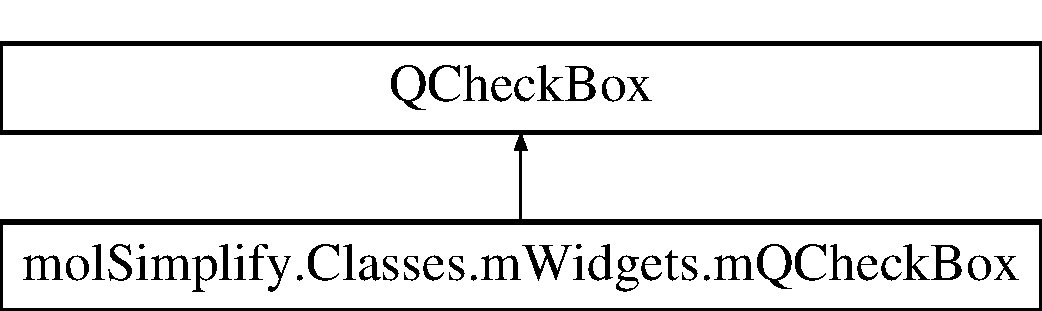
\includegraphics[height=2.000000cm]{classmolSimplify_1_1Classes_1_1mWidgets_1_1mQCheckBox}
\end{center}
\end{figure}
\subsection*{Public Member Functions}
\begin{DoxyCompactItemize}
\item 
def \hyperlink{classmolSimplify_1_1Classes_1_1mWidgets_1_1mQCheckBox_a487010e1018e3e7f6df83279dbf86ac9}{\+\_\+\+\_\+init\+\_\+\+\_\+} (self, txt, ctip, fontsize)
\item 
def \hyperlink{classmolSimplify_1_1Classes_1_1mWidgets_1_1mQCheckBox_ab7bae41eb0c34231e7d00df846c8da7a}{changestate} (self)
\item 
def \hyperlink{classmolSimplify_1_1Classes_1_1mWidgets_1_1mQCheckBox_a2f135c915ecfafd92d834b7e38606f93}{get\+State} (self)
\end{DoxyCompactItemize}
\subsection*{Public Attributes}
\begin{DoxyCompactItemize}
\item 
\hyperlink{classmolSimplify_1_1Classes_1_1mWidgets_1_1mQCheckBox_aceae51b12d02f3680795e1d8baa27c44}{state}
\end{DoxyCompactItemize}


\subsection{Detailed Description}
G\+UI checkbox class. 

\subsection{Constructor \& Destructor Documentation}
\mbox{\Hypertarget{classmolSimplify_1_1Classes_1_1mWidgets_1_1mQCheckBox_a487010e1018e3e7f6df83279dbf86ac9}\label{classmolSimplify_1_1Classes_1_1mWidgets_1_1mQCheckBox_a487010e1018e3e7f6df83279dbf86ac9}} 
\index{mol\+Simplify\+::\+Classes\+::m\+Widgets\+::m\+Q\+Check\+Box@{mol\+Simplify\+::\+Classes\+::m\+Widgets\+::m\+Q\+Check\+Box}!\+\_\+\+\_\+init\+\_\+\+\_\+@{\+\_\+\+\_\+init\+\_\+\+\_\+}}
\index{\+\_\+\+\_\+init\+\_\+\+\_\+@{\+\_\+\+\_\+init\+\_\+\+\_\+}!mol\+Simplify\+::\+Classes\+::m\+Widgets\+::m\+Q\+Check\+Box@{mol\+Simplify\+::\+Classes\+::m\+Widgets\+::m\+Q\+Check\+Box}}
\subsubsection{\texorpdfstring{\+\_\+\+\_\+init\+\_\+\+\_\+()}{\_\_init\_\_()}}
{\footnotesize\ttfamily def mol\+Simplify.\+Classes.\+m\+Widgets.\+m\+Q\+Check\+Box.\+\_\+\+\_\+init\+\_\+\+\_\+ (\begin{DoxyParamCaption}\item[{}]{self,  }\item[{}]{txt,  }\item[{}]{ctip,  }\item[{}]{fontsize }\end{DoxyParamCaption})}



\subsection{Member Function Documentation}
\mbox{\Hypertarget{classmolSimplify_1_1Classes_1_1mWidgets_1_1mQCheckBox_ab7bae41eb0c34231e7d00df846c8da7a}\label{classmolSimplify_1_1Classes_1_1mWidgets_1_1mQCheckBox_ab7bae41eb0c34231e7d00df846c8da7a}} 
\index{mol\+Simplify\+::\+Classes\+::m\+Widgets\+::m\+Q\+Check\+Box@{mol\+Simplify\+::\+Classes\+::m\+Widgets\+::m\+Q\+Check\+Box}!changestate@{changestate}}
\index{changestate@{changestate}!mol\+Simplify\+::\+Classes\+::m\+Widgets\+::m\+Q\+Check\+Box@{mol\+Simplify\+::\+Classes\+::m\+Widgets\+::m\+Q\+Check\+Box}}
\subsubsection{\texorpdfstring{changestate()}{changestate()}}
{\footnotesize\ttfamily def mol\+Simplify.\+Classes.\+m\+Widgets.\+m\+Q\+Check\+Box.\+changestate (\begin{DoxyParamCaption}\item[{}]{self }\end{DoxyParamCaption})}

\mbox{\Hypertarget{classmolSimplify_1_1Classes_1_1mWidgets_1_1mQCheckBox_a2f135c915ecfafd92d834b7e38606f93}\label{classmolSimplify_1_1Classes_1_1mWidgets_1_1mQCheckBox_a2f135c915ecfafd92d834b7e38606f93}} 
\index{mol\+Simplify\+::\+Classes\+::m\+Widgets\+::m\+Q\+Check\+Box@{mol\+Simplify\+::\+Classes\+::m\+Widgets\+::m\+Q\+Check\+Box}!get\+State@{get\+State}}
\index{get\+State@{get\+State}!mol\+Simplify\+::\+Classes\+::m\+Widgets\+::m\+Q\+Check\+Box@{mol\+Simplify\+::\+Classes\+::m\+Widgets\+::m\+Q\+Check\+Box}}
\subsubsection{\texorpdfstring{get\+State()}{getState()}}
{\footnotesize\ttfamily def mol\+Simplify.\+Classes.\+m\+Widgets.\+m\+Q\+Check\+Box.\+get\+State (\begin{DoxyParamCaption}\item[{}]{self }\end{DoxyParamCaption})}



\subsection{Member Data Documentation}
\mbox{\Hypertarget{classmolSimplify_1_1Classes_1_1mWidgets_1_1mQCheckBox_aceae51b12d02f3680795e1d8baa27c44}\label{classmolSimplify_1_1Classes_1_1mWidgets_1_1mQCheckBox_aceae51b12d02f3680795e1d8baa27c44}} 
\index{mol\+Simplify\+::\+Classes\+::m\+Widgets\+::m\+Q\+Check\+Box@{mol\+Simplify\+::\+Classes\+::m\+Widgets\+::m\+Q\+Check\+Box}!state@{state}}
\index{state@{state}!mol\+Simplify\+::\+Classes\+::m\+Widgets\+::m\+Q\+Check\+Box@{mol\+Simplify\+::\+Classes\+::m\+Widgets\+::m\+Q\+Check\+Box}}
\subsubsection{\texorpdfstring{state}{state}}
{\footnotesize\ttfamily mol\+Simplify.\+Classes.\+m\+Widgets.\+m\+Q\+Check\+Box.\+state}



The documentation for this class was generated from the following file\+:\begin{DoxyCompactItemize}
\item 
Classes/\hyperlink{mWidgets_8py}{m\+Widgets.\+py}\end{DoxyCompactItemize}

\hypertarget{classmolSimplify_1_1Classes_1_1mWidgets_1_1mQComboBox}{}\section{mol\+Simplify.\+Classes.\+m\+Widgets.\+m\+Q\+Combo\+Box Class Reference}
\label{classmolSimplify_1_1Classes_1_1mWidgets_1_1mQComboBox}\index{mol\+Simplify.\+Classes.\+m\+Widgets.\+m\+Q\+Combo\+Box@{mol\+Simplify.\+Classes.\+m\+Widgets.\+m\+Q\+Combo\+Box}}


G\+UI dropdown box class.  


Inheritance diagram for mol\+Simplify.\+Classes.\+m\+Widgets.\+m\+Q\+Combo\+Box\+:\begin{figure}[H]
\begin{center}
\leavevmode
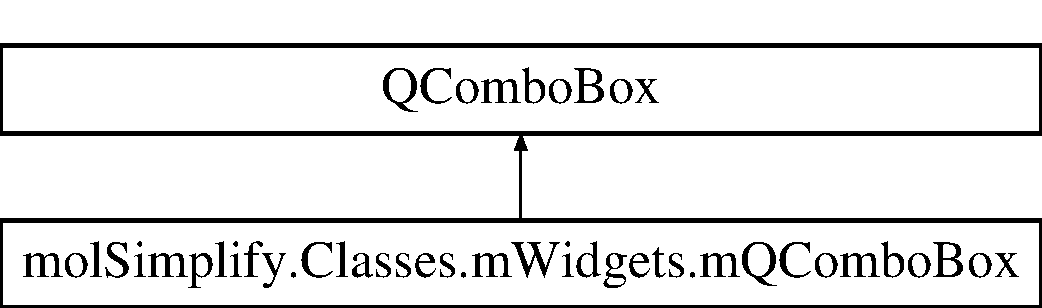
\includegraphics[height=2.000000cm]{classmolSimplify_1_1Classes_1_1mWidgets_1_1mQComboBox}
\end{center}
\end{figure}
\subsection*{Public Member Functions}
\begin{DoxyCompactItemize}
\item 
def \hyperlink{classmolSimplify_1_1Classes_1_1mWidgets_1_1mQComboBox_afaf4adf57e88ad34e4bf69665618df03}{\+\_\+\+\_\+init\+\_\+\+\_\+} (self, txt, ctip, fontsize)
\item 
def \hyperlink{classmolSimplify_1_1Classes_1_1mWidgets_1_1mQComboBox_a72f40806a96a8090899cdfdb7f52cff7}{get\+State} (self)
\item 
def \hyperlink{classmolSimplify_1_1Classes_1_1mWidgets_1_1mQComboBox_ab9644845237e3c327c353e4d27058755}{get\+Text} (self)
\end{DoxyCompactItemize}
\subsection*{Public Attributes}
\begin{DoxyCompactItemize}
\item 
\hyperlink{classmolSimplify_1_1Classes_1_1mWidgets_1_1mQComboBox_a58df656e7910be7e97773966dc068e8e}{state}
\end{DoxyCompactItemize}


\subsection{Detailed Description}
G\+UI dropdown box class. 

\subsection{Constructor \& Destructor Documentation}
\mbox{\Hypertarget{classmolSimplify_1_1Classes_1_1mWidgets_1_1mQComboBox_afaf4adf57e88ad34e4bf69665618df03}\label{classmolSimplify_1_1Classes_1_1mWidgets_1_1mQComboBox_afaf4adf57e88ad34e4bf69665618df03}} 
\index{mol\+Simplify\+::\+Classes\+::m\+Widgets\+::m\+Q\+Combo\+Box@{mol\+Simplify\+::\+Classes\+::m\+Widgets\+::m\+Q\+Combo\+Box}!\+\_\+\+\_\+init\+\_\+\+\_\+@{\+\_\+\+\_\+init\+\_\+\+\_\+}}
\index{\+\_\+\+\_\+init\+\_\+\+\_\+@{\+\_\+\+\_\+init\+\_\+\+\_\+}!mol\+Simplify\+::\+Classes\+::m\+Widgets\+::m\+Q\+Combo\+Box@{mol\+Simplify\+::\+Classes\+::m\+Widgets\+::m\+Q\+Combo\+Box}}
\subsubsection{\texorpdfstring{\+\_\+\+\_\+init\+\_\+\+\_\+()}{\_\_init\_\_()}}
{\footnotesize\ttfamily def mol\+Simplify.\+Classes.\+m\+Widgets.\+m\+Q\+Combo\+Box.\+\_\+\+\_\+init\+\_\+\+\_\+ (\begin{DoxyParamCaption}\item[{}]{self,  }\item[{}]{txt,  }\item[{}]{ctip,  }\item[{}]{fontsize }\end{DoxyParamCaption})}



\subsection{Member Function Documentation}
\mbox{\Hypertarget{classmolSimplify_1_1Classes_1_1mWidgets_1_1mQComboBox_a72f40806a96a8090899cdfdb7f52cff7}\label{classmolSimplify_1_1Classes_1_1mWidgets_1_1mQComboBox_a72f40806a96a8090899cdfdb7f52cff7}} 
\index{mol\+Simplify\+::\+Classes\+::m\+Widgets\+::m\+Q\+Combo\+Box@{mol\+Simplify\+::\+Classes\+::m\+Widgets\+::m\+Q\+Combo\+Box}!get\+State@{get\+State}}
\index{get\+State@{get\+State}!mol\+Simplify\+::\+Classes\+::m\+Widgets\+::m\+Q\+Combo\+Box@{mol\+Simplify\+::\+Classes\+::m\+Widgets\+::m\+Q\+Combo\+Box}}
\subsubsection{\texorpdfstring{get\+State()}{getState()}}
{\footnotesize\ttfamily def mol\+Simplify.\+Classes.\+m\+Widgets.\+m\+Q\+Combo\+Box.\+get\+State (\begin{DoxyParamCaption}\item[{}]{self }\end{DoxyParamCaption})}

\mbox{\Hypertarget{classmolSimplify_1_1Classes_1_1mWidgets_1_1mQComboBox_ab9644845237e3c327c353e4d27058755}\label{classmolSimplify_1_1Classes_1_1mWidgets_1_1mQComboBox_ab9644845237e3c327c353e4d27058755}} 
\index{mol\+Simplify\+::\+Classes\+::m\+Widgets\+::m\+Q\+Combo\+Box@{mol\+Simplify\+::\+Classes\+::m\+Widgets\+::m\+Q\+Combo\+Box}!get\+Text@{get\+Text}}
\index{get\+Text@{get\+Text}!mol\+Simplify\+::\+Classes\+::m\+Widgets\+::m\+Q\+Combo\+Box@{mol\+Simplify\+::\+Classes\+::m\+Widgets\+::m\+Q\+Combo\+Box}}
\subsubsection{\texorpdfstring{get\+Text()}{getText()}}
{\footnotesize\ttfamily def mol\+Simplify.\+Classes.\+m\+Widgets.\+m\+Q\+Combo\+Box.\+get\+Text (\begin{DoxyParamCaption}\item[{}]{self }\end{DoxyParamCaption})}



\subsection{Member Data Documentation}
\mbox{\Hypertarget{classmolSimplify_1_1Classes_1_1mWidgets_1_1mQComboBox_a58df656e7910be7e97773966dc068e8e}\label{classmolSimplify_1_1Classes_1_1mWidgets_1_1mQComboBox_a58df656e7910be7e97773966dc068e8e}} 
\index{mol\+Simplify\+::\+Classes\+::m\+Widgets\+::m\+Q\+Combo\+Box@{mol\+Simplify\+::\+Classes\+::m\+Widgets\+::m\+Q\+Combo\+Box}!state@{state}}
\index{state@{state}!mol\+Simplify\+::\+Classes\+::m\+Widgets\+::m\+Q\+Combo\+Box@{mol\+Simplify\+::\+Classes\+::m\+Widgets\+::m\+Q\+Combo\+Box}}
\subsubsection{\texorpdfstring{state}{state}}
{\footnotesize\ttfamily mol\+Simplify.\+Classes.\+m\+Widgets.\+m\+Q\+Combo\+Box.\+state}



The documentation for this class was generated from the following file\+:\begin{DoxyCompactItemize}
\item 
Classes/\hyperlink{mWidgets_8py}{m\+Widgets.\+py}\end{DoxyCompactItemize}

\hypertarget{classmolSimplify_1_1Classes_1_1mWidgets_1_1mQDialogErr}{}\section{mol\+Simplify.\+Classes.\+m\+Widgets.\+m\+Q\+Dialog\+Err Class Reference}
\label{classmolSimplify_1_1Classes_1_1mWidgets_1_1mQDialogErr}\index{mol\+Simplify.\+Classes.\+m\+Widgets.\+m\+Q\+Dialog\+Err@{mol\+Simplify.\+Classes.\+m\+Widgets.\+m\+Q\+Dialog\+Err}}


G\+UI error dialog box class.  


Inheritance diagram for mol\+Simplify.\+Classes.\+m\+Widgets.\+m\+Q\+Dialog\+Err\+:\begin{figure}[H]
\begin{center}
\leavevmode
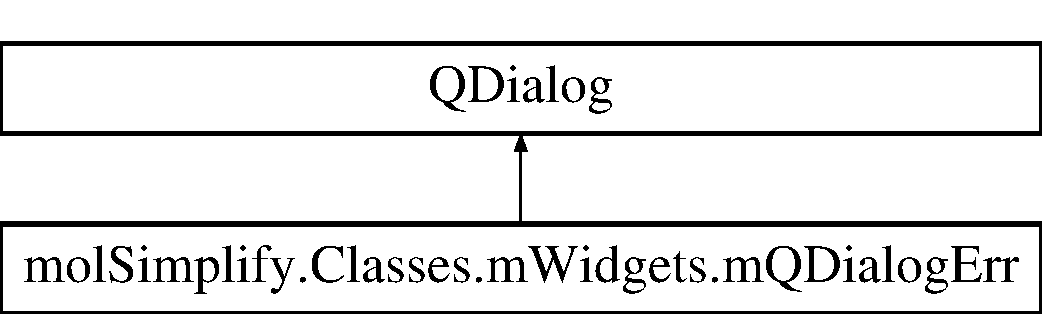
\includegraphics[height=2.000000cm]{classmolSimplify_1_1Classes_1_1mWidgets_1_1mQDialogErr}
\end{center}
\end{figure}
\subsection*{Public Member Functions}
\begin{DoxyCompactItemize}
\item 
def \hyperlink{classmolSimplify_1_1Classes_1_1mWidgets_1_1mQDialogErr_a46f42e7b843eead634804993b34a6f60}{\+\_\+\+\_\+init\+\_\+\+\_\+} (self, toptxt, txt)
\end{DoxyCompactItemize}
\subsection*{Public Attributes}
\begin{DoxyCompactItemize}
\item 
\hyperlink{classmolSimplify_1_1Classes_1_1mWidgets_1_1mQDialogErr_a7cd18fb34503fbea7ef86c42dde7de4c}{msg\+Box}
\end{DoxyCompactItemize}


\subsection{Detailed Description}
G\+UI error dialog box class. 

\subsection{Constructor \& Destructor Documentation}
\mbox{\Hypertarget{classmolSimplify_1_1Classes_1_1mWidgets_1_1mQDialogErr_a46f42e7b843eead634804993b34a6f60}\label{classmolSimplify_1_1Classes_1_1mWidgets_1_1mQDialogErr_a46f42e7b843eead634804993b34a6f60}} 
\index{mol\+Simplify\+::\+Classes\+::m\+Widgets\+::m\+Q\+Dialog\+Err@{mol\+Simplify\+::\+Classes\+::m\+Widgets\+::m\+Q\+Dialog\+Err}!\+\_\+\+\_\+init\+\_\+\+\_\+@{\+\_\+\+\_\+init\+\_\+\+\_\+}}
\index{\+\_\+\+\_\+init\+\_\+\+\_\+@{\+\_\+\+\_\+init\+\_\+\+\_\+}!mol\+Simplify\+::\+Classes\+::m\+Widgets\+::m\+Q\+Dialog\+Err@{mol\+Simplify\+::\+Classes\+::m\+Widgets\+::m\+Q\+Dialog\+Err}}
\subsubsection{\texorpdfstring{\+\_\+\+\_\+init\+\_\+\+\_\+()}{\_\_init\_\_()}}
{\footnotesize\ttfamily def mol\+Simplify.\+Classes.\+m\+Widgets.\+m\+Q\+Dialog\+Err.\+\_\+\+\_\+init\+\_\+\+\_\+ (\begin{DoxyParamCaption}\item[{}]{self,  }\item[{}]{toptxt,  }\item[{}]{txt }\end{DoxyParamCaption})}



\subsection{Member Data Documentation}
\mbox{\Hypertarget{classmolSimplify_1_1Classes_1_1mWidgets_1_1mQDialogErr_a7cd18fb34503fbea7ef86c42dde7de4c}\label{classmolSimplify_1_1Classes_1_1mWidgets_1_1mQDialogErr_a7cd18fb34503fbea7ef86c42dde7de4c}} 
\index{mol\+Simplify\+::\+Classes\+::m\+Widgets\+::m\+Q\+Dialog\+Err@{mol\+Simplify\+::\+Classes\+::m\+Widgets\+::m\+Q\+Dialog\+Err}!msg\+Box@{msg\+Box}}
\index{msg\+Box@{msg\+Box}!mol\+Simplify\+::\+Classes\+::m\+Widgets\+::m\+Q\+Dialog\+Err@{mol\+Simplify\+::\+Classes\+::m\+Widgets\+::m\+Q\+Dialog\+Err}}
\subsubsection{\texorpdfstring{msg\+Box}{msgBox}}
{\footnotesize\ttfamily mol\+Simplify.\+Classes.\+m\+Widgets.\+m\+Q\+Dialog\+Err.\+msg\+Box}



The documentation for this class was generated from the following file\+:\begin{DoxyCompactItemize}
\item 
Classes/\hyperlink{mWidgets_8py}{m\+Widgets.\+py}\end{DoxyCompactItemize}

\hypertarget{classmolSimplify_1_1Classes_1_1mWidgets_1_1mQDialogInf}{}\section{mol\+Simplify.\+Classes.\+m\+Widgets.\+m\+Q\+Dialog\+Inf Class Reference}
\label{classmolSimplify_1_1Classes_1_1mWidgets_1_1mQDialogInf}\index{mol\+Simplify.\+Classes.\+m\+Widgets.\+m\+Q\+Dialog\+Inf@{mol\+Simplify.\+Classes.\+m\+Widgets.\+m\+Q\+Dialog\+Inf}}


G\+UI popup boxes class.  


Inheritance diagram for mol\+Simplify.\+Classes.\+m\+Widgets.\+m\+Q\+Dialog\+Inf\+:\begin{figure}[H]
\begin{center}
\leavevmode
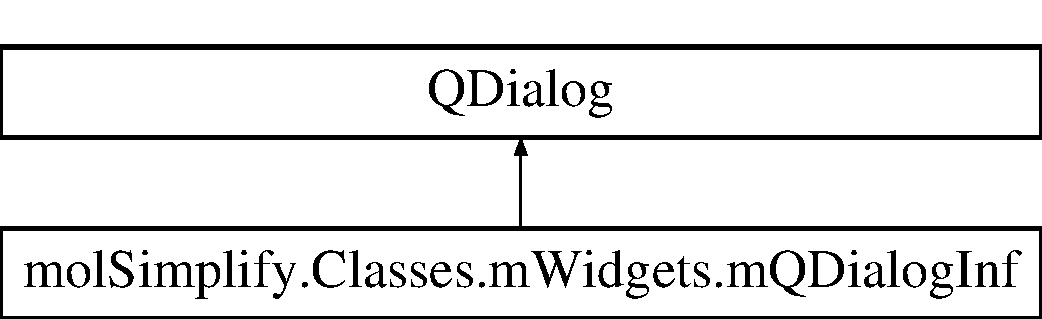
\includegraphics[height=2.000000cm]{classmolSimplify_1_1Classes_1_1mWidgets_1_1mQDialogInf}
\end{center}
\end{figure}
\subsection*{Public Member Functions}
\begin{DoxyCompactItemize}
\item 
def \hyperlink{classmolSimplify_1_1Classes_1_1mWidgets_1_1mQDialogInf_a99b2338263f4ace549f5d873ba3bb544}{\+\_\+\+\_\+init\+\_\+\+\_\+} (self, toptxt, txt)
\end{DoxyCompactItemize}
\subsection*{Public Attributes}
\begin{DoxyCompactItemize}
\item 
\hyperlink{classmolSimplify_1_1Classes_1_1mWidgets_1_1mQDialogInf_a745462b985bfaeafa1603f5567505bd3}{msg\+Box}
\end{DoxyCompactItemize}


\subsection{Detailed Description}
G\+UI popup boxes class. 

\subsection{Constructor \& Destructor Documentation}
\mbox{\Hypertarget{classmolSimplify_1_1Classes_1_1mWidgets_1_1mQDialogInf_a99b2338263f4ace549f5d873ba3bb544}\label{classmolSimplify_1_1Classes_1_1mWidgets_1_1mQDialogInf_a99b2338263f4ace549f5d873ba3bb544}} 
\index{mol\+Simplify\+::\+Classes\+::m\+Widgets\+::m\+Q\+Dialog\+Inf@{mol\+Simplify\+::\+Classes\+::m\+Widgets\+::m\+Q\+Dialog\+Inf}!\+\_\+\+\_\+init\+\_\+\+\_\+@{\+\_\+\+\_\+init\+\_\+\+\_\+}}
\index{\+\_\+\+\_\+init\+\_\+\+\_\+@{\+\_\+\+\_\+init\+\_\+\+\_\+}!mol\+Simplify\+::\+Classes\+::m\+Widgets\+::m\+Q\+Dialog\+Inf@{mol\+Simplify\+::\+Classes\+::m\+Widgets\+::m\+Q\+Dialog\+Inf}}
\subsubsection{\texorpdfstring{\+\_\+\+\_\+init\+\_\+\+\_\+()}{\_\_init\_\_()}}
{\footnotesize\ttfamily def mol\+Simplify.\+Classes.\+m\+Widgets.\+m\+Q\+Dialog\+Inf.\+\_\+\+\_\+init\+\_\+\+\_\+ (\begin{DoxyParamCaption}\item[{}]{self,  }\item[{}]{toptxt,  }\item[{}]{txt }\end{DoxyParamCaption})}



\subsection{Member Data Documentation}
\mbox{\Hypertarget{classmolSimplify_1_1Classes_1_1mWidgets_1_1mQDialogInf_a745462b985bfaeafa1603f5567505bd3}\label{classmolSimplify_1_1Classes_1_1mWidgets_1_1mQDialogInf_a745462b985bfaeafa1603f5567505bd3}} 
\index{mol\+Simplify\+::\+Classes\+::m\+Widgets\+::m\+Q\+Dialog\+Inf@{mol\+Simplify\+::\+Classes\+::m\+Widgets\+::m\+Q\+Dialog\+Inf}!msg\+Box@{msg\+Box}}
\index{msg\+Box@{msg\+Box}!mol\+Simplify\+::\+Classes\+::m\+Widgets\+::m\+Q\+Dialog\+Inf@{mol\+Simplify\+::\+Classes\+::m\+Widgets\+::m\+Q\+Dialog\+Inf}}
\subsubsection{\texorpdfstring{msg\+Box}{msgBox}}
{\footnotesize\ttfamily mol\+Simplify.\+Classes.\+m\+Widgets.\+m\+Q\+Dialog\+Inf.\+msg\+Box}



The documentation for this class was generated from the following file\+:\begin{DoxyCompactItemize}
\item 
Classes/\hyperlink{mWidgets_8py}{m\+Widgets.\+py}\end{DoxyCompactItemize}

\hypertarget{classmolSimplify_1_1Classes_1_1mWidgets_1_1mQDialogWarn}{}\section{mol\+Simplify.\+Classes.\+m\+Widgets.\+m\+Q\+Dialog\+Warn Class Reference}
\label{classmolSimplify_1_1Classes_1_1mWidgets_1_1mQDialogWarn}\index{mol\+Simplify.\+Classes.\+m\+Widgets.\+m\+Q\+Dialog\+Warn@{mol\+Simplify.\+Classes.\+m\+Widgets.\+m\+Q\+Dialog\+Warn}}


G\+UI warning dialog box class.  


Inheritance diagram for mol\+Simplify.\+Classes.\+m\+Widgets.\+m\+Q\+Dialog\+Warn\+:\begin{figure}[H]
\begin{center}
\leavevmode
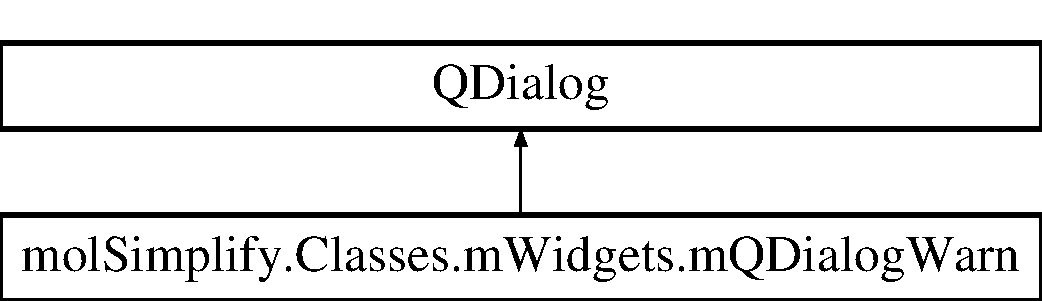
\includegraphics[height=2.000000cm]{classmolSimplify_1_1Classes_1_1mWidgets_1_1mQDialogWarn}
\end{center}
\end{figure}
\subsection*{Public Member Functions}
\begin{DoxyCompactItemize}
\item 
def \hyperlink{classmolSimplify_1_1Classes_1_1mWidgets_1_1mQDialogWarn_a2f01dd2838544bad680c22949810207a}{\+\_\+\+\_\+init\+\_\+\+\_\+} (self, toptxt, txt)
\end{DoxyCompactItemize}
\subsection*{Public Attributes}
\begin{DoxyCompactItemize}
\item 
\hyperlink{classmolSimplify_1_1Classes_1_1mWidgets_1_1mQDialogWarn_a70da02558109736f726fe3945081d0cd}{msg\+Box}
\end{DoxyCompactItemize}


\subsection{Detailed Description}
G\+UI warning dialog box class. 

\subsection{Constructor \& Destructor Documentation}
\mbox{\Hypertarget{classmolSimplify_1_1Classes_1_1mWidgets_1_1mQDialogWarn_a2f01dd2838544bad680c22949810207a}\label{classmolSimplify_1_1Classes_1_1mWidgets_1_1mQDialogWarn_a2f01dd2838544bad680c22949810207a}} 
\index{mol\+Simplify\+::\+Classes\+::m\+Widgets\+::m\+Q\+Dialog\+Warn@{mol\+Simplify\+::\+Classes\+::m\+Widgets\+::m\+Q\+Dialog\+Warn}!\+\_\+\+\_\+init\+\_\+\+\_\+@{\+\_\+\+\_\+init\+\_\+\+\_\+}}
\index{\+\_\+\+\_\+init\+\_\+\+\_\+@{\+\_\+\+\_\+init\+\_\+\+\_\+}!mol\+Simplify\+::\+Classes\+::m\+Widgets\+::m\+Q\+Dialog\+Warn@{mol\+Simplify\+::\+Classes\+::m\+Widgets\+::m\+Q\+Dialog\+Warn}}
\subsubsection{\texorpdfstring{\+\_\+\+\_\+init\+\_\+\+\_\+()}{\_\_init\_\_()}}
{\footnotesize\ttfamily def mol\+Simplify.\+Classes.\+m\+Widgets.\+m\+Q\+Dialog\+Warn.\+\_\+\+\_\+init\+\_\+\+\_\+ (\begin{DoxyParamCaption}\item[{}]{self,  }\item[{}]{toptxt,  }\item[{}]{txt }\end{DoxyParamCaption})}



\subsection{Member Data Documentation}
\mbox{\Hypertarget{classmolSimplify_1_1Classes_1_1mWidgets_1_1mQDialogWarn_a70da02558109736f726fe3945081d0cd}\label{classmolSimplify_1_1Classes_1_1mWidgets_1_1mQDialogWarn_a70da02558109736f726fe3945081d0cd}} 
\index{mol\+Simplify\+::\+Classes\+::m\+Widgets\+::m\+Q\+Dialog\+Warn@{mol\+Simplify\+::\+Classes\+::m\+Widgets\+::m\+Q\+Dialog\+Warn}!msg\+Box@{msg\+Box}}
\index{msg\+Box@{msg\+Box}!mol\+Simplify\+::\+Classes\+::m\+Widgets\+::m\+Q\+Dialog\+Warn@{mol\+Simplify\+::\+Classes\+::m\+Widgets\+::m\+Q\+Dialog\+Warn}}
\subsubsection{\texorpdfstring{msg\+Box}{msgBox}}
{\footnotesize\ttfamily mol\+Simplify.\+Classes.\+m\+Widgets.\+m\+Q\+Dialog\+Warn.\+msg\+Box}



The documentation for this class was generated from the following file\+:\begin{DoxyCompactItemize}
\item 
Classes/\hyperlink{mWidgets_8py}{m\+Widgets.\+py}\end{DoxyCompactItemize}

\hypertarget{classmolSimplify_1_1Classes_1_1mWidgets_1_1mQLabel}{}\section{mol\+Simplify.\+Classes.\+m\+Widgets.\+m\+Q\+Label Class Reference}
\label{classmolSimplify_1_1Classes_1_1mWidgets_1_1mQLabel}\index{mol\+Simplify.\+Classes.\+m\+Widgets.\+m\+Q\+Label@{mol\+Simplify.\+Classes.\+m\+Widgets.\+m\+Q\+Label}}


G\+UI static texts class.  


Inheritance diagram for mol\+Simplify.\+Classes.\+m\+Widgets.\+m\+Q\+Label\+:\begin{figure}[H]
\begin{center}
\leavevmode
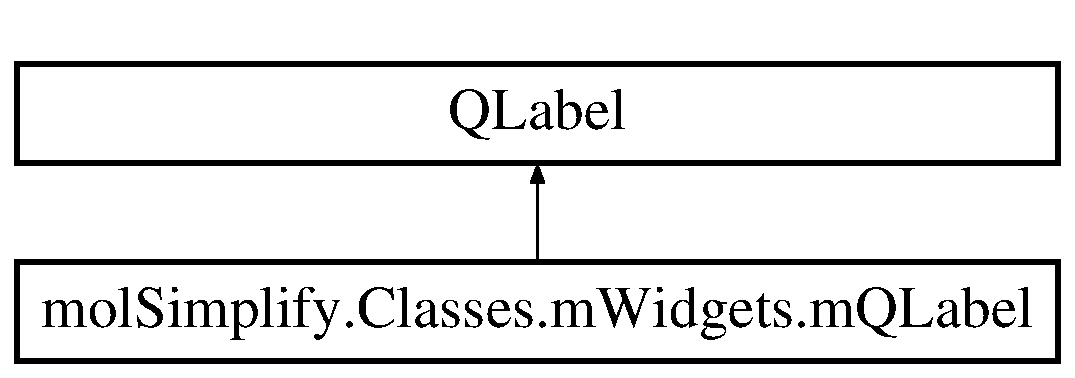
\includegraphics[height=2.000000cm]{classmolSimplify_1_1Classes_1_1mWidgets_1_1mQLabel}
\end{center}
\end{figure}
\subsection*{Public Member Functions}
\begin{DoxyCompactItemize}
\item 
def \hyperlink{classmolSimplify_1_1Classes_1_1mWidgets_1_1mQLabel_aefeede684761e86741538bbe607600dc}{\+\_\+\+\_\+init\+\_\+\+\_\+} (self, txt, ctip, align, fontsize)
\item 
def \hyperlink{classmolSimplify_1_1Classes_1_1mWidgets_1_1mQLabel_ac4b868e52cbb2ef6f8974cef329f6dba}{resize2\+Event} (self, event)
\end{DoxyCompactItemize}


\subsection{Detailed Description}
G\+UI static texts class. 

\subsection{Constructor \& Destructor Documentation}
\mbox{\Hypertarget{classmolSimplify_1_1Classes_1_1mWidgets_1_1mQLabel_aefeede684761e86741538bbe607600dc}\label{classmolSimplify_1_1Classes_1_1mWidgets_1_1mQLabel_aefeede684761e86741538bbe607600dc}} 
\index{mol\+Simplify\+::\+Classes\+::m\+Widgets\+::m\+Q\+Label@{mol\+Simplify\+::\+Classes\+::m\+Widgets\+::m\+Q\+Label}!\+\_\+\+\_\+init\+\_\+\+\_\+@{\+\_\+\+\_\+init\+\_\+\+\_\+}}
\index{\+\_\+\+\_\+init\+\_\+\+\_\+@{\+\_\+\+\_\+init\+\_\+\+\_\+}!mol\+Simplify\+::\+Classes\+::m\+Widgets\+::m\+Q\+Label@{mol\+Simplify\+::\+Classes\+::m\+Widgets\+::m\+Q\+Label}}
\subsubsection{\texorpdfstring{\+\_\+\+\_\+init\+\_\+\+\_\+()}{\_\_init\_\_()}}
{\footnotesize\ttfamily def mol\+Simplify.\+Classes.\+m\+Widgets.\+m\+Q\+Label.\+\_\+\+\_\+init\+\_\+\+\_\+ (\begin{DoxyParamCaption}\item[{}]{self,  }\item[{}]{txt,  }\item[{}]{ctip,  }\item[{}]{align,  }\item[{}]{fontsize }\end{DoxyParamCaption})}



\subsection{Member Function Documentation}
\mbox{\Hypertarget{classmolSimplify_1_1Classes_1_1mWidgets_1_1mQLabel_ac4b868e52cbb2ef6f8974cef329f6dba}\label{classmolSimplify_1_1Classes_1_1mWidgets_1_1mQLabel_ac4b868e52cbb2ef6f8974cef329f6dba}} 
\index{mol\+Simplify\+::\+Classes\+::m\+Widgets\+::m\+Q\+Label@{mol\+Simplify\+::\+Classes\+::m\+Widgets\+::m\+Q\+Label}!resize2\+Event@{resize2\+Event}}
\index{resize2\+Event@{resize2\+Event}!mol\+Simplify\+::\+Classes\+::m\+Widgets\+::m\+Q\+Label@{mol\+Simplify\+::\+Classes\+::m\+Widgets\+::m\+Q\+Label}}
\subsubsection{\texorpdfstring{resize2\+Event()}{resize2Event()}}
{\footnotesize\ttfamily def mol\+Simplify.\+Classes.\+m\+Widgets.\+m\+Q\+Label.\+resize2\+Event (\begin{DoxyParamCaption}\item[{}]{self,  }\item[{}]{event }\end{DoxyParamCaption})}



The documentation for this class was generated from the following file\+:\begin{DoxyCompactItemize}
\item 
Classes/\hyperlink{mWidgets_8py}{m\+Widgets.\+py}\end{DoxyCompactItemize}

\hypertarget{classmolSimplify_1_1Classes_1_1mWidgets_1_1mQLineEdit}{}\section{mol\+Simplify.\+Classes.\+m\+Widgets.\+m\+Q\+Line\+Edit Class Reference}
\label{classmolSimplify_1_1Classes_1_1mWidgets_1_1mQLineEdit}\index{mol\+Simplify.\+Classes.\+m\+Widgets.\+m\+Q\+Line\+Edit@{mol\+Simplify.\+Classes.\+m\+Widgets.\+m\+Q\+Line\+Edit}}


G\+UI edit texts class.  


Inheritance diagram for mol\+Simplify.\+Classes.\+m\+Widgets.\+m\+Q\+Line\+Edit\+:\begin{figure}[H]
\begin{center}
\leavevmode
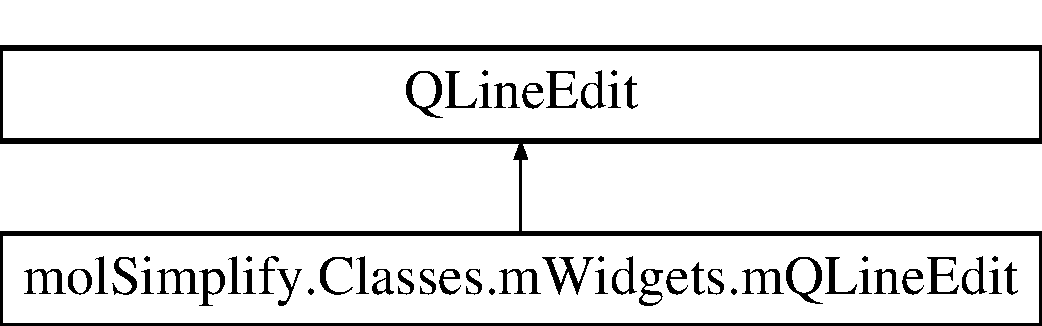
\includegraphics[height=2.000000cm]{classmolSimplify_1_1Classes_1_1mWidgets_1_1mQLineEdit}
\end{center}
\end{figure}
\subsection*{Public Member Functions}
\begin{DoxyCompactItemize}
\item 
def \hyperlink{classmolSimplify_1_1Classes_1_1mWidgets_1_1mQLineEdit_a136a1b549a57a9cc1fd996851bc3269c}{\+\_\+\+\_\+init\+\_\+\+\_\+} (self, txt, ctip, align, fontsize)
\end{DoxyCompactItemize}


\subsection{Detailed Description}
G\+UI edit texts class. 

\subsection{Constructor \& Destructor Documentation}
\mbox{\Hypertarget{classmolSimplify_1_1Classes_1_1mWidgets_1_1mQLineEdit_a136a1b549a57a9cc1fd996851bc3269c}\label{classmolSimplify_1_1Classes_1_1mWidgets_1_1mQLineEdit_a136a1b549a57a9cc1fd996851bc3269c}} 
\index{mol\+Simplify\+::\+Classes\+::m\+Widgets\+::m\+Q\+Line\+Edit@{mol\+Simplify\+::\+Classes\+::m\+Widgets\+::m\+Q\+Line\+Edit}!\+\_\+\+\_\+init\+\_\+\+\_\+@{\+\_\+\+\_\+init\+\_\+\+\_\+}}
\index{\+\_\+\+\_\+init\+\_\+\+\_\+@{\+\_\+\+\_\+init\+\_\+\+\_\+}!mol\+Simplify\+::\+Classes\+::m\+Widgets\+::m\+Q\+Line\+Edit@{mol\+Simplify\+::\+Classes\+::m\+Widgets\+::m\+Q\+Line\+Edit}}
\subsubsection{\texorpdfstring{\+\_\+\+\_\+init\+\_\+\+\_\+()}{\_\_init\_\_()}}
{\footnotesize\ttfamily def mol\+Simplify.\+Classes.\+m\+Widgets.\+m\+Q\+Line\+Edit.\+\_\+\+\_\+init\+\_\+\+\_\+ (\begin{DoxyParamCaption}\item[{}]{self,  }\item[{}]{txt,  }\item[{}]{ctip,  }\item[{}]{align,  }\item[{}]{fontsize }\end{DoxyParamCaption})}



The documentation for this class was generated from the following file\+:\begin{DoxyCompactItemize}
\item 
Classes/\hyperlink{mWidgets_8py}{m\+Widgets.\+py}\end{DoxyCompactItemize}

\hypertarget{classmolSimplify_1_1Classes_1_1mWidgets_1_1mQLineEditL}{}\section{mol\+Simplify.\+Classes.\+m\+Widgets.\+m\+Q\+Line\+EditL Class Reference}
\label{classmolSimplify_1_1Classes_1_1mWidgets_1_1mQLineEditL}\index{mol\+Simplify.\+Classes.\+m\+Widgets.\+m\+Q\+Line\+EditL@{mol\+Simplify.\+Classes.\+m\+Widgets.\+m\+Q\+Line\+EditL}}


Another G\+UI edit texts class.  


Inheritance diagram for mol\+Simplify.\+Classes.\+m\+Widgets.\+m\+Q\+Line\+EditL\+:\begin{figure}[H]
\begin{center}
\leavevmode
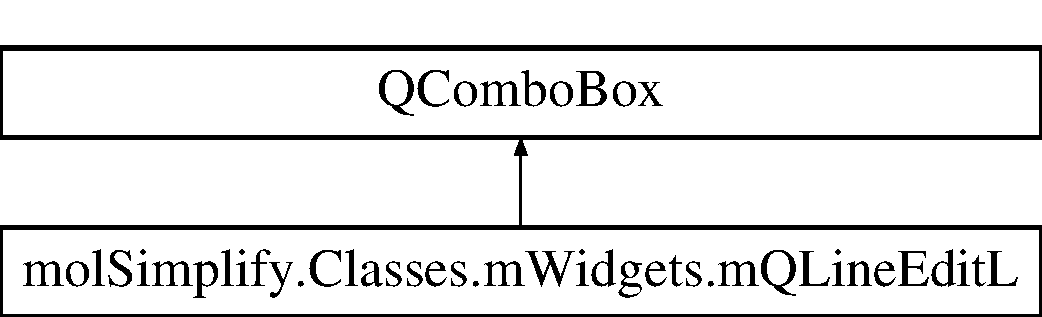
\includegraphics[height=2.000000cm]{classmolSimplify_1_1Classes_1_1mWidgets_1_1mQLineEditL}
\end{center}
\end{figure}
\subsection*{Public Member Functions}
\begin{DoxyCompactItemize}
\item 
def \hyperlink{classmolSimplify_1_1Classes_1_1mWidgets_1_1mQLineEditL_a4ec14adb6debfce9e6c5fefa5a411ed2}{\+\_\+\+\_\+init\+\_\+\+\_\+} (self, txt, ctip, align, fontsize, licores)
\item 
def \hyperlink{classmolSimplify_1_1Classes_1_1mWidgets_1_1mQLineEditL_a0928b280d95373379db84fb7303a9582}{on\+\_\+completer\+\_\+activated} (self, text)
\end{DoxyCompactItemize}
\subsection*{Public Attributes}
\begin{DoxyCompactItemize}
\item 
\hyperlink{classmolSimplify_1_1Classes_1_1mWidgets_1_1mQLineEditL_a97b91fb79b6396c63b495333569300c3}{p\+Filter\+Model}
\item 
\hyperlink{classmolSimplify_1_1Classes_1_1mWidgets_1_1mQLineEditL_a957e9facab3d5870125767a2de4993ec}{completer}
\end{DoxyCompactItemize}


\subsection{Detailed Description}
Another G\+UI edit texts class. 

\subsection{Constructor \& Destructor Documentation}
\mbox{\Hypertarget{classmolSimplify_1_1Classes_1_1mWidgets_1_1mQLineEditL_a4ec14adb6debfce9e6c5fefa5a411ed2}\label{classmolSimplify_1_1Classes_1_1mWidgets_1_1mQLineEditL_a4ec14adb6debfce9e6c5fefa5a411ed2}} 
\index{mol\+Simplify\+::\+Classes\+::m\+Widgets\+::m\+Q\+Line\+EditL@{mol\+Simplify\+::\+Classes\+::m\+Widgets\+::m\+Q\+Line\+EditL}!\+\_\+\+\_\+init\+\_\+\+\_\+@{\+\_\+\+\_\+init\+\_\+\+\_\+}}
\index{\+\_\+\+\_\+init\+\_\+\+\_\+@{\+\_\+\+\_\+init\+\_\+\+\_\+}!mol\+Simplify\+::\+Classes\+::m\+Widgets\+::m\+Q\+Line\+EditL@{mol\+Simplify\+::\+Classes\+::m\+Widgets\+::m\+Q\+Line\+EditL}}
\subsubsection{\texorpdfstring{\+\_\+\+\_\+init\+\_\+\+\_\+()}{\_\_init\_\_()}}
{\footnotesize\ttfamily def mol\+Simplify.\+Classes.\+m\+Widgets.\+m\+Q\+Line\+Edit\+L.\+\_\+\+\_\+init\+\_\+\+\_\+ (\begin{DoxyParamCaption}\item[{}]{self,  }\item[{}]{txt,  }\item[{}]{ctip,  }\item[{}]{align,  }\item[{}]{fontsize,  }\item[{}]{licores }\end{DoxyParamCaption})}



\subsection{Member Function Documentation}
\mbox{\Hypertarget{classmolSimplify_1_1Classes_1_1mWidgets_1_1mQLineEditL_a0928b280d95373379db84fb7303a9582}\label{classmolSimplify_1_1Classes_1_1mWidgets_1_1mQLineEditL_a0928b280d95373379db84fb7303a9582}} 
\index{mol\+Simplify\+::\+Classes\+::m\+Widgets\+::m\+Q\+Line\+EditL@{mol\+Simplify\+::\+Classes\+::m\+Widgets\+::m\+Q\+Line\+EditL}!on\+\_\+completer\+\_\+activated@{on\+\_\+completer\+\_\+activated}}
\index{on\+\_\+completer\+\_\+activated@{on\+\_\+completer\+\_\+activated}!mol\+Simplify\+::\+Classes\+::m\+Widgets\+::m\+Q\+Line\+EditL@{mol\+Simplify\+::\+Classes\+::m\+Widgets\+::m\+Q\+Line\+EditL}}
\subsubsection{\texorpdfstring{on\+\_\+completer\+\_\+activated()}{on\_completer\_activated()}}
{\footnotesize\ttfamily def mol\+Simplify.\+Classes.\+m\+Widgets.\+m\+Q\+Line\+Edit\+L.\+on\+\_\+completer\+\_\+activated (\begin{DoxyParamCaption}\item[{}]{self,  }\item[{}]{text }\end{DoxyParamCaption})}



\subsection{Member Data Documentation}
\mbox{\Hypertarget{classmolSimplify_1_1Classes_1_1mWidgets_1_1mQLineEditL_a957e9facab3d5870125767a2de4993ec}\label{classmolSimplify_1_1Classes_1_1mWidgets_1_1mQLineEditL_a957e9facab3d5870125767a2de4993ec}} 
\index{mol\+Simplify\+::\+Classes\+::m\+Widgets\+::m\+Q\+Line\+EditL@{mol\+Simplify\+::\+Classes\+::m\+Widgets\+::m\+Q\+Line\+EditL}!completer@{completer}}
\index{completer@{completer}!mol\+Simplify\+::\+Classes\+::m\+Widgets\+::m\+Q\+Line\+EditL@{mol\+Simplify\+::\+Classes\+::m\+Widgets\+::m\+Q\+Line\+EditL}}
\subsubsection{\texorpdfstring{completer}{completer}}
{\footnotesize\ttfamily mol\+Simplify.\+Classes.\+m\+Widgets.\+m\+Q\+Line\+Edit\+L.\+completer}

\mbox{\Hypertarget{classmolSimplify_1_1Classes_1_1mWidgets_1_1mQLineEditL_a97b91fb79b6396c63b495333569300c3}\label{classmolSimplify_1_1Classes_1_1mWidgets_1_1mQLineEditL_a97b91fb79b6396c63b495333569300c3}} 
\index{mol\+Simplify\+::\+Classes\+::m\+Widgets\+::m\+Q\+Line\+EditL@{mol\+Simplify\+::\+Classes\+::m\+Widgets\+::m\+Q\+Line\+EditL}!p\+Filter\+Model@{p\+Filter\+Model}}
\index{p\+Filter\+Model@{p\+Filter\+Model}!mol\+Simplify\+::\+Classes\+::m\+Widgets\+::m\+Q\+Line\+EditL@{mol\+Simplify\+::\+Classes\+::m\+Widgets\+::m\+Q\+Line\+EditL}}
\subsubsection{\texorpdfstring{p\+Filter\+Model}{pFilterModel}}
{\footnotesize\ttfamily mol\+Simplify.\+Classes.\+m\+Widgets.\+m\+Q\+Line\+Edit\+L.\+p\+Filter\+Model}



The documentation for this class was generated from the following file\+:\begin{DoxyCompactItemize}
\item 
Classes/\hyperlink{mWidgets_8py}{m\+Widgets.\+py}\end{DoxyCompactItemize}

\hypertarget{classmolSimplify_1_1Classes_1_1mWidgets_1_1mQMainWindow}{}\section{mol\+Simplify.\+Classes.\+m\+Widgets.\+m\+Q\+Main\+Window Class Reference}
\label{classmolSimplify_1_1Classes_1_1mWidgets_1_1mQMainWindow}\index{mol\+Simplify.\+Classes.\+m\+Widgets.\+m\+Q\+Main\+Window@{mol\+Simplify.\+Classes.\+m\+Widgets.\+m\+Q\+Main\+Window}}


G\+UI main window class.  


Inheritance diagram for mol\+Simplify.\+Classes.\+m\+Widgets.\+m\+Q\+Main\+Window\+:\begin{figure}[H]
\begin{center}
\leavevmode
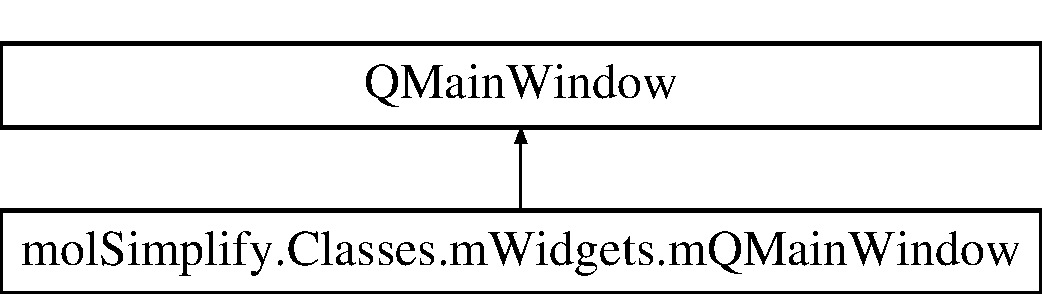
\includegraphics[height=2.000000cm]{classmolSimplify_1_1Classes_1_1mWidgets_1_1mQMainWindow}
\end{center}
\end{figure}
\subsection*{Public Member Functions}
\begin{DoxyCompactItemize}
\item 
def \hyperlink{classmolSimplify_1_1Classes_1_1mWidgets_1_1mQMainWindow_a501a2616567a0a203495409b3e76689b}{\+\_\+\+\_\+init\+\_\+\+\_\+} (self)
\item 
def \hyperlink{classmolSimplify_1_1Classes_1_1mWidgets_1_1mQMainWindow_ad056877a48172e3cdb203fb822058234}{close\+Event} (self, event)
\end{DoxyCompactItemize}


\subsection{Detailed Description}
G\+UI main window class. 

\subsection{Constructor \& Destructor Documentation}
\mbox{\Hypertarget{classmolSimplify_1_1Classes_1_1mWidgets_1_1mQMainWindow_a501a2616567a0a203495409b3e76689b}\label{classmolSimplify_1_1Classes_1_1mWidgets_1_1mQMainWindow_a501a2616567a0a203495409b3e76689b}} 
\index{mol\+Simplify\+::\+Classes\+::m\+Widgets\+::m\+Q\+Main\+Window@{mol\+Simplify\+::\+Classes\+::m\+Widgets\+::m\+Q\+Main\+Window}!\+\_\+\+\_\+init\+\_\+\+\_\+@{\+\_\+\+\_\+init\+\_\+\+\_\+}}
\index{\+\_\+\+\_\+init\+\_\+\+\_\+@{\+\_\+\+\_\+init\+\_\+\+\_\+}!mol\+Simplify\+::\+Classes\+::m\+Widgets\+::m\+Q\+Main\+Window@{mol\+Simplify\+::\+Classes\+::m\+Widgets\+::m\+Q\+Main\+Window}}
\subsubsection{\texorpdfstring{\+\_\+\+\_\+init\+\_\+\+\_\+()}{\_\_init\_\_()}}
{\footnotesize\ttfamily def mol\+Simplify.\+Classes.\+m\+Widgets.\+m\+Q\+Main\+Window.\+\_\+\+\_\+init\+\_\+\+\_\+ (\begin{DoxyParamCaption}\item[{}]{self }\end{DoxyParamCaption})}



\subsection{Member Function Documentation}
\mbox{\Hypertarget{classmolSimplify_1_1Classes_1_1mWidgets_1_1mQMainWindow_ad056877a48172e3cdb203fb822058234}\label{classmolSimplify_1_1Classes_1_1mWidgets_1_1mQMainWindow_ad056877a48172e3cdb203fb822058234}} 
\index{mol\+Simplify\+::\+Classes\+::m\+Widgets\+::m\+Q\+Main\+Window@{mol\+Simplify\+::\+Classes\+::m\+Widgets\+::m\+Q\+Main\+Window}!close\+Event@{close\+Event}}
\index{close\+Event@{close\+Event}!mol\+Simplify\+::\+Classes\+::m\+Widgets\+::m\+Q\+Main\+Window@{mol\+Simplify\+::\+Classes\+::m\+Widgets\+::m\+Q\+Main\+Window}}
\subsubsection{\texorpdfstring{close\+Event()}{closeEvent()}}
{\footnotesize\ttfamily def mol\+Simplify.\+Classes.\+m\+Widgets.\+m\+Q\+Main\+Window.\+close\+Event (\begin{DoxyParamCaption}\item[{}]{self,  }\item[{}]{event }\end{DoxyParamCaption})}



The documentation for this class was generated from the following file\+:\begin{DoxyCompactItemize}
\item 
Classes/\hyperlink{mWidgets_8py}{m\+Widgets.\+py}\end{DoxyCompactItemize}

\hypertarget{classmolSimplify_1_1Classes_1_1mWidgets_1_1mQMessageBox}{}\section{mol\+Simplify.\+Classes.\+m\+Widgets.\+m\+Q\+Message\+Box Class Reference}
\label{classmolSimplify_1_1Classes_1_1mWidgets_1_1mQMessageBox}\index{mol\+Simplify.\+Classes.\+m\+Widgets.\+m\+Q\+Message\+Box@{mol\+Simplify.\+Classes.\+m\+Widgets.\+m\+Q\+Message\+Box}}


G\+UI message box class.  


Inheritance diagram for mol\+Simplify.\+Classes.\+m\+Widgets.\+m\+Q\+Message\+Box\+:\begin{figure}[H]
\begin{center}
\leavevmode
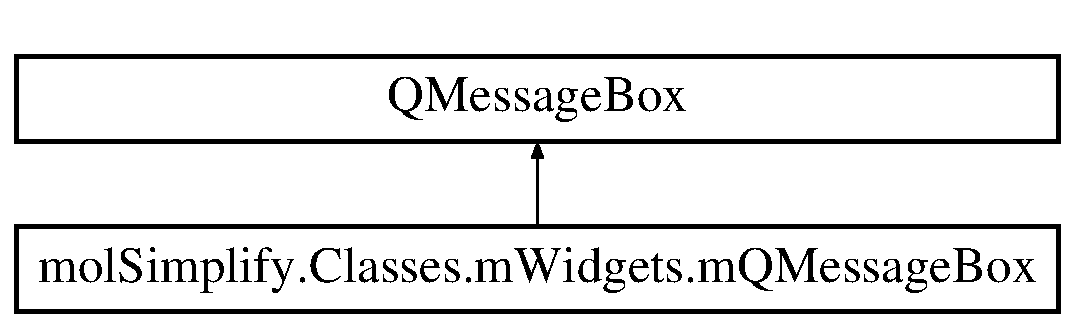
\includegraphics[height=2.000000cm]{classmolSimplify_1_1Classes_1_1mWidgets_1_1mQMessageBox}
\end{center}
\end{figure}
\subsection*{Public Member Functions}
\begin{DoxyCompactItemize}
\item 
def \hyperlink{classmolSimplify_1_1Classes_1_1mWidgets_1_1mQMessageBox_a41a5c729e25eee8d1cfd9ec661567a68}{\+\_\+\+\_\+init\+\_\+\+\_\+} (self, title, text, typ, \hyperlink{classmolSimplify_1_1Classes_1_1mWidgets_1_1mQMessageBox_a72e0288a3ae9c22560124d97cdaa93e2}{autoclose})
\item 
def \hyperlink{classmolSimplify_1_1Classes_1_1mWidgets_1_1mQMessageBox_ac04dd28ad94321c6f561f7ca38c0a3c6}{show\+Event} (self, event)
\end{DoxyCompactItemize}
\subsection*{Public Attributes}
\begin{DoxyCompactItemize}
\item 
\hyperlink{classmolSimplify_1_1Classes_1_1mWidgets_1_1mQMessageBox_a72e0288a3ae9c22560124d97cdaa93e2}{autoclose}
\end{DoxyCompactItemize}


\subsection{Detailed Description}
G\+UI message box class. 

\subsection{Constructor \& Destructor Documentation}
\mbox{\Hypertarget{classmolSimplify_1_1Classes_1_1mWidgets_1_1mQMessageBox_a41a5c729e25eee8d1cfd9ec661567a68}\label{classmolSimplify_1_1Classes_1_1mWidgets_1_1mQMessageBox_a41a5c729e25eee8d1cfd9ec661567a68}} 
\index{mol\+Simplify\+::\+Classes\+::m\+Widgets\+::m\+Q\+Message\+Box@{mol\+Simplify\+::\+Classes\+::m\+Widgets\+::m\+Q\+Message\+Box}!\+\_\+\+\_\+init\+\_\+\+\_\+@{\+\_\+\+\_\+init\+\_\+\+\_\+}}
\index{\+\_\+\+\_\+init\+\_\+\+\_\+@{\+\_\+\+\_\+init\+\_\+\+\_\+}!mol\+Simplify\+::\+Classes\+::m\+Widgets\+::m\+Q\+Message\+Box@{mol\+Simplify\+::\+Classes\+::m\+Widgets\+::m\+Q\+Message\+Box}}
\subsubsection{\texorpdfstring{\+\_\+\+\_\+init\+\_\+\+\_\+()}{\_\_init\_\_()}}
{\footnotesize\ttfamily def mol\+Simplify.\+Classes.\+m\+Widgets.\+m\+Q\+Message\+Box.\+\_\+\+\_\+init\+\_\+\+\_\+ (\begin{DoxyParamCaption}\item[{}]{self,  }\item[{}]{title,  }\item[{}]{text,  }\item[{}]{typ,  }\item[{}]{autoclose }\end{DoxyParamCaption})}



\subsection{Member Function Documentation}
\mbox{\Hypertarget{classmolSimplify_1_1Classes_1_1mWidgets_1_1mQMessageBox_ac04dd28ad94321c6f561f7ca38c0a3c6}\label{classmolSimplify_1_1Classes_1_1mWidgets_1_1mQMessageBox_ac04dd28ad94321c6f561f7ca38c0a3c6}} 
\index{mol\+Simplify\+::\+Classes\+::m\+Widgets\+::m\+Q\+Message\+Box@{mol\+Simplify\+::\+Classes\+::m\+Widgets\+::m\+Q\+Message\+Box}!show\+Event@{show\+Event}}
\index{show\+Event@{show\+Event}!mol\+Simplify\+::\+Classes\+::m\+Widgets\+::m\+Q\+Message\+Box@{mol\+Simplify\+::\+Classes\+::m\+Widgets\+::m\+Q\+Message\+Box}}
\subsubsection{\texorpdfstring{show\+Event()}{showEvent()}}
{\footnotesize\ttfamily def mol\+Simplify.\+Classes.\+m\+Widgets.\+m\+Q\+Message\+Box.\+show\+Event (\begin{DoxyParamCaption}\item[{}]{self,  }\item[{}]{event }\end{DoxyParamCaption})}



\subsection{Member Data Documentation}
\mbox{\Hypertarget{classmolSimplify_1_1Classes_1_1mWidgets_1_1mQMessageBox_a72e0288a3ae9c22560124d97cdaa93e2}\label{classmolSimplify_1_1Classes_1_1mWidgets_1_1mQMessageBox_a72e0288a3ae9c22560124d97cdaa93e2}} 
\index{mol\+Simplify\+::\+Classes\+::m\+Widgets\+::m\+Q\+Message\+Box@{mol\+Simplify\+::\+Classes\+::m\+Widgets\+::m\+Q\+Message\+Box}!autoclose@{autoclose}}
\index{autoclose@{autoclose}!mol\+Simplify\+::\+Classes\+::m\+Widgets\+::m\+Q\+Message\+Box@{mol\+Simplify\+::\+Classes\+::m\+Widgets\+::m\+Q\+Message\+Box}}
\subsubsection{\texorpdfstring{autoclose}{autoclose}}
{\footnotesize\ttfamily mol\+Simplify.\+Classes.\+m\+Widgets.\+m\+Q\+Message\+Box.\+autoclose}



The documentation for this class was generated from the following file\+:\begin{DoxyCompactItemize}
\item 
Classes/\hyperlink{mWidgets_8py}{m\+Widgets.\+py}\end{DoxyCompactItemize}

\hypertarget{classmolSimplify_1_1Classes_1_1mWidgets_1_1mQPixmap}{}\section{mol\+Simplify.\+Classes.\+m\+Widgets.\+m\+Q\+Pixmap Class Reference}
\label{classmolSimplify_1_1Classes_1_1mWidgets_1_1mQPixmap}\index{mol\+Simplify.\+Classes.\+m\+Widgets.\+m\+Q\+Pixmap@{mol\+Simplify.\+Classes.\+m\+Widgets.\+m\+Q\+Pixmap}}


G\+UI pixmap class.  


Inheritance diagram for mol\+Simplify.\+Classes.\+m\+Widgets.\+m\+Q\+Pixmap\+:\begin{figure}[H]
\begin{center}
\leavevmode
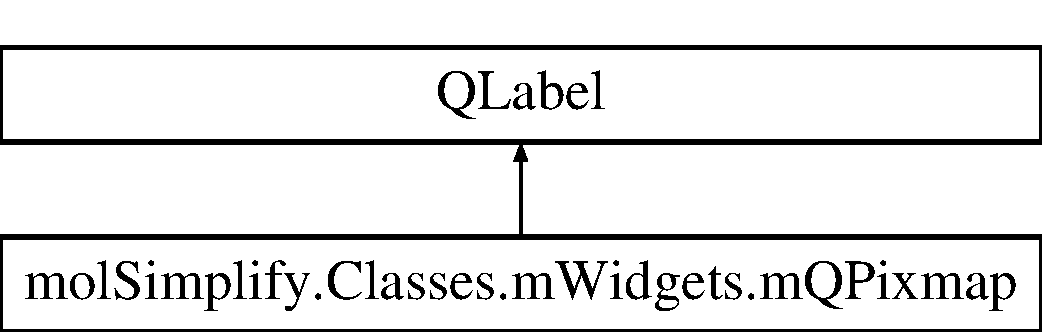
\includegraphics[height=2.000000cm]{classmolSimplify_1_1Classes_1_1mWidgets_1_1mQPixmap}
\end{center}
\end{figure}
\subsection*{Public Member Functions}
\begin{DoxyCompactItemize}
\item 
def \hyperlink{classmolSimplify_1_1Classes_1_1mWidgets_1_1mQPixmap_aaf933090efd42e5db66472904527163e}{\+\_\+\+\_\+init\+\_\+\+\_\+} (self, picpath)
\item 
def \hyperlink{classmolSimplify_1_1Classes_1_1mWidgets_1_1mQPixmap_a5bc5a8cecbaa770e2020f21c0dc67bcc}{resize\+Event} (self, event)
\end{DoxyCompactItemize}
\subsection*{Public Attributes}
\begin{DoxyCompactItemize}
\item 
\hyperlink{classmolSimplify_1_1Classes_1_1mWidgets_1_1mQPixmap_a375741d56a1de4780e51396e682c89fb}{pixmap}
\end{DoxyCompactItemize}


\subsection{Detailed Description}
G\+UI pixmap class. 

\subsection{Constructor \& Destructor Documentation}
\mbox{\Hypertarget{classmolSimplify_1_1Classes_1_1mWidgets_1_1mQPixmap_aaf933090efd42e5db66472904527163e}\label{classmolSimplify_1_1Classes_1_1mWidgets_1_1mQPixmap_aaf933090efd42e5db66472904527163e}} 
\index{mol\+Simplify\+::\+Classes\+::m\+Widgets\+::m\+Q\+Pixmap@{mol\+Simplify\+::\+Classes\+::m\+Widgets\+::m\+Q\+Pixmap}!\+\_\+\+\_\+init\+\_\+\+\_\+@{\+\_\+\+\_\+init\+\_\+\+\_\+}}
\index{\+\_\+\+\_\+init\+\_\+\+\_\+@{\+\_\+\+\_\+init\+\_\+\+\_\+}!mol\+Simplify\+::\+Classes\+::m\+Widgets\+::m\+Q\+Pixmap@{mol\+Simplify\+::\+Classes\+::m\+Widgets\+::m\+Q\+Pixmap}}
\subsubsection{\texorpdfstring{\+\_\+\+\_\+init\+\_\+\+\_\+()}{\_\_init\_\_()}}
{\footnotesize\ttfamily def mol\+Simplify.\+Classes.\+m\+Widgets.\+m\+Q\+Pixmap.\+\_\+\+\_\+init\+\_\+\+\_\+ (\begin{DoxyParamCaption}\item[{}]{self,  }\item[{}]{picpath }\end{DoxyParamCaption})}



\subsection{Member Function Documentation}
\mbox{\Hypertarget{classmolSimplify_1_1Classes_1_1mWidgets_1_1mQPixmap_a5bc5a8cecbaa770e2020f21c0dc67bcc}\label{classmolSimplify_1_1Classes_1_1mWidgets_1_1mQPixmap_a5bc5a8cecbaa770e2020f21c0dc67bcc}} 
\index{mol\+Simplify\+::\+Classes\+::m\+Widgets\+::m\+Q\+Pixmap@{mol\+Simplify\+::\+Classes\+::m\+Widgets\+::m\+Q\+Pixmap}!resize\+Event@{resize\+Event}}
\index{resize\+Event@{resize\+Event}!mol\+Simplify\+::\+Classes\+::m\+Widgets\+::m\+Q\+Pixmap@{mol\+Simplify\+::\+Classes\+::m\+Widgets\+::m\+Q\+Pixmap}}
\subsubsection{\texorpdfstring{resize\+Event()}{resizeEvent()}}
{\footnotesize\ttfamily def mol\+Simplify.\+Classes.\+m\+Widgets.\+m\+Q\+Pixmap.\+resize\+Event (\begin{DoxyParamCaption}\item[{}]{self,  }\item[{}]{event }\end{DoxyParamCaption})}



\subsection{Member Data Documentation}
\mbox{\Hypertarget{classmolSimplify_1_1Classes_1_1mWidgets_1_1mQPixmap_a375741d56a1de4780e51396e682c89fb}\label{classmolSimplify_1_1Classes_1_1mWidgets_1_1mQPixmap_a375741d56a1de4780e51396e682c89fb}} 
\index{mol\+Simplify\+::\+Classes\+::m\+Widgets\+::m\+Q\+Pixmap@{mol\+Simplify\+::\+Classes\+::m\+Widgets\+::m\+Q\+Pixmap}!pixmap@{pixmap}}
\index{pixmap@{pixmap}!mol\+Simplify\+::\+Classes\+::m\+Widgets\+::m\+Q\+Pixmap@{mol\+Simplify\+::\+Classes\+::m\+Widgets\+::m\+Q\+Pixmap}}
\subsubsection{\texorpdfstring{pixmap}{pixmap}}
{\footnotesize\ttfamily mol\+Simplify.\+Classes.\+m\+Widgets.\+m\+Q\+Pixmap.\+pixmap}



The documentation for this class was generated from the following file\+:\begin{DoxyCompactItemize}
\item 
Classes/\hyperlink{mWidgets_8py}{m\+Widgets.\+py}\end{DoxyCompactItemize}

\hypertarget{classmolSimplify_1_1Classes_1_1mWidgets_1_1mQPushButton}{}\section{mol\+Simplify.\+Classes.\+m\+Widgets.\+m\+Q\+Push\+Button Class Reference}
\label{classmolSimplify_1_1Classes_1_1mWidgets_1_1mQPushButton}\index{mol\+Simplify.\+Classes.\+m\+Widgets.\+m\+Q\+Push\+Button@{mol\+Simplify.\+Classes.\+m\+Widgets.\+m\+Q\+Push\+Button}}


G\+UI push button class.  


Inheritance diagram for mol\+Simplify.\+Classes.\+m\+Widgets.\+m\+Q\+Push\+Button\+:\begin{figure}[H]
\begin{center}
\leavevmode
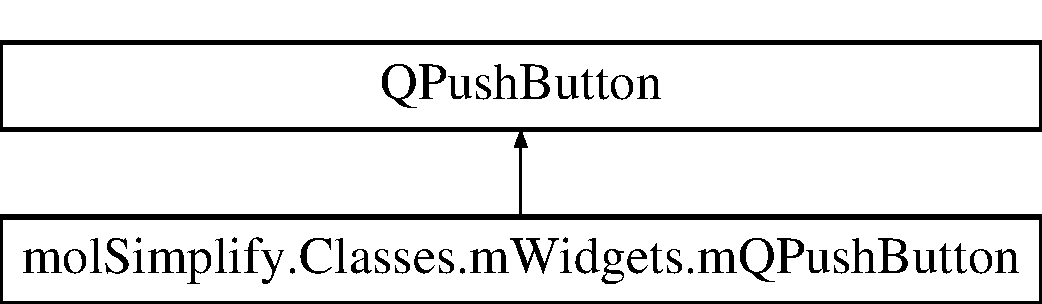
\includegraphics[height=2.000000cm]{classmolSimplify_1_1Classes_1_1mWidgets_1_1mQPushButton}
\end{center}
\end{figure}
\subsection*{Public Member Functions}
\begin{DoxyCompactItemize}
\item 
def \hyperlink{classmolSimplify_1_1Classes_1_1mWidgets_1_1mQPushButton_a814a6963cdc08ee2eb6e6db70182fd85}{\+\_\+\+\_\+init\+\_\+\+\_\+} (self, txt, ctip, fontsize)
\end{DoxyCompactItemize}


\subsection{Detailed Description}
G\+UI push button class. 

\subsection{Constructor \& Destructor Documentation}
\mbox{\Hypertarget{classmolSimplify_1_1Classes_1_1mWidgets_1_1mQPushButton_a814a6963cdc08ee2eb6e6db70182fd85}\label{classmolSimplify_1_1Classes_1_1mWidgets_1_1mQPushButton_a814a6963cdc08ee2eb6e6db70182fd85}} 
\index{mol\+Simplify\+::\+Classes\+::m\+Widgets\+::m\+Q\+Push\+Button@{mol\+Simplify\+::\+Classes\+::m\+Widgets\+::m\+Q\+Push\+Button}!\+\_\+\+\_\+init\+\_\+\+\_\+@{\+\_\+\+\_\+init\+\_\+\+\_\+}}
\index{\+\_\+\+\_\+init\+\_\+\+\_\+@{\+\_\+\+\_\+init\+\_\+\+\_\+}!mol\+Simplify\+::\+Classes\+::m\+Widgets\+::m\+Q\+Push\+Button@{mol\+Simplify\+::\+Classes\+::m\+Widgets\+::m\+Q\+Push\+Button}}
\subsubsection{\texorpdfstring{\+\_\+\+\_\+init\+\_\+\+\_\+()}{\_\_init\_\_()}}
{\footnotesize\ttfamily def mol\+Simplify.\+Classes.\+m\+Widgets.\+m\+Q\+Push\+Button.\+\_\+\+\_\+init\+\_\+\+\_\+ (\begin{DoxyParamCaption}\item[{}]{self,  }\item[{}]{txt,  }\item[{}]{ctip,  }\item[{}]{fontsize }\end{DoxyParamCaption})}



The documentation for this class was generated from the following file\+:\begin{DoxyCompactItemize}
\item 
Classes/\hyperlink{mWidgets_8py}{m\+Widgets.\+py}\end{DoxyCompactItemize}

\hypertarget{classmolSimplify_1_1Classes_1_1mWidgets_1_1mQSlider}{}\section{mol\+Simplify.\+Classes.\+m\+Widgets.\+m\+Q\+Slider Class Reference}
\label{classmolSimplify_1_1Classes_1_1mWidgets_1_1mQSlider}\index{mol\+Simplify.\+Classes.\+m\+Widgets.\+m\+Q\+Slider@{mol\+Simplify.\+Classes.\+m\+Widgets.\+m\+Q\+Slider}}


G\+UI slider class.  


Inheritance diagram for mol\+Simplify.\+Classes.\+m\+Widgets.\+m\+Q\+Slider\+:\begin{figure}[H]
\begin{center}
\leavevmode
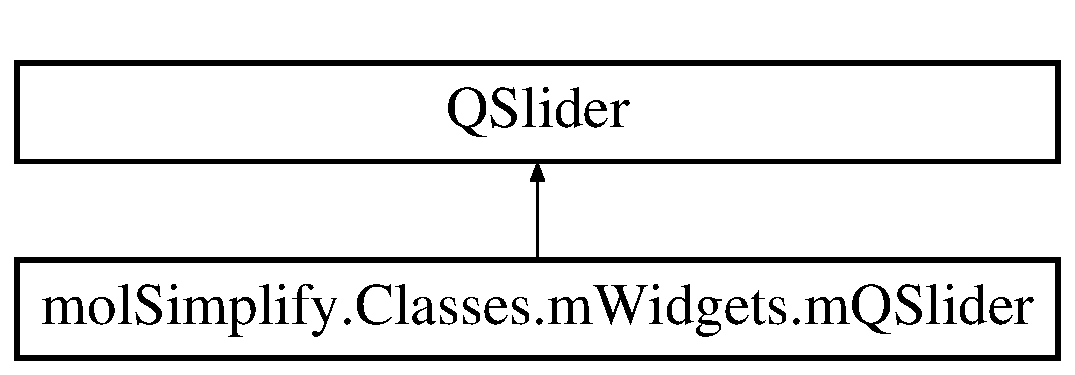
\includegraphics[height=2.000000cm]{classmolSimplify_1_1Classes_1_1mWidgets_1_1mQSlider}
\end{center}
\end{figure}
\subsection*{Public Member Functions}
\begin{DoxyCompactItemize}
\item 
def \hyperlink{classmolSimplify_1_1Classes_1_1mWidgets_1_1mQSlider_a73ea6d61500daa421d1e9ae108a56f01}{\+\_\+\+\_\+init\+\_\+\+\_\+} (self, ctip)
\end{DoxyCompactItemize}


\subsection{Detailed Description}
G\+UI slider class. 

\subsection{Constructor \& Destructor Documentation}
\mbox{\Hypertarget{classmolSimplify_1_1Classes_1_1mWidgets_1_1mQSlider_a73ea6d61500daa421d1e9ae108a56f01}\label{classmolSimplify_1_1Classes_1_1mWidgets_1_1mQSlider_a73ea6d61500daa421d1e9ae108a56f01}} 
\index{mol\+Simplify\+::\+Classes\+::m\+Widgets\+::m\+Q\+Slider@{mol\+Simplify\+::\+Classes\+::m\+Widgets\+::m\+Q\+Slider}!\+\_\+\+\_\+init\+\_\+\+\_\+@{\+\_\+\+\_\+init\+\_\+\+\_\+}}
\index{\+\_\+\+\_\+init\+\_\+\+\_\+@{\+\_\+\+\_\+init\+\_\+\+\_\+}!mol\+Simplify\+::\+Classes\+::m\+Widgets\+::m\+Q\+Slider@{mol\+Simplify\+::\+Classes\+::m\+Widgets\+::m\+Q\+Slider}}
\subsubsection{\texorpdfstring{\+\_\+\+\_\+init\+\_\+\+\_\+()}{\_\_init\_\_()}}
{\footnotesize\ttfamily def mol\+Simplify.\+Classes.\+m\+Widgets.\+m\+Q\+Slider.\+\_\+\+\_\+init\+\_\+\+\_\+ (\begin{DoxyParamCaption}\item[{}]{self,  }\item[{}]{ctip }\end{DoxyParamCaption})}



The documentation for this class was generated from the following file\+:\begin{DoxyCompactItemize}
\item 
Classes/\hyperlink{mWidgets_8py}{m\+Widgets.\+py}\end{DoxyCompactItemize}

\hypertarget{classmolSimplify_1_1Classes_1_1mWidgets_1_1mQSpinBox}{}\section{mol\+Simplify.\+Classes.\+m\+Widgets.\+m\+Q\+Spin\+Box Class Reference}
\label{classmolSimplify_1_1Classes_1_1mWidgets_1_1mQSpinBox}\index{mol\+Simplify.\+Classes.\+m\+Widgets.\+m\+Q\+Spin\+Box@{mol\+Simplify.\+Classes.\+m\+Widgets.\+m\+Q\+Spin\+Box}}


G\+UI spin box class.  


Inheritance diagram for mol\+Simplify.\+Classes.\+m\+Widgets.\+m\+Q\+Spin\+Box\+:\begin{figure}[H]
\begin{center}
\leavevmode
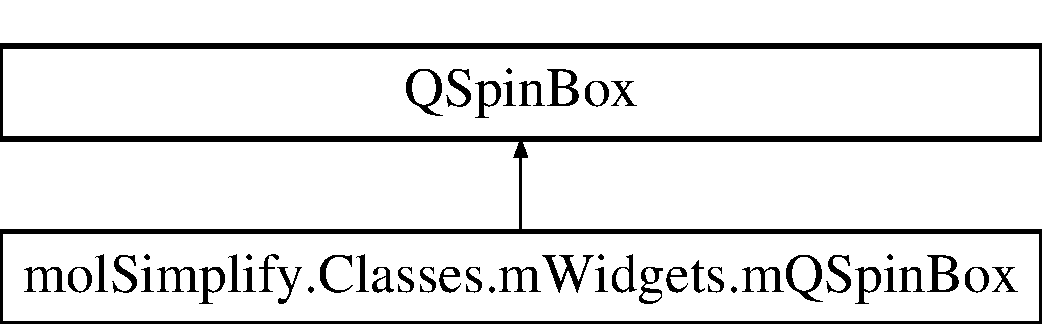
\includegraphics[height=2.000000cm]{classmolSimplify_1_1Classes_1_1mWidgets_1_1mQSpinBox}
\end{center}
\end{figure}
\subsection*{Public Member Functions}
\begin{DoxyCompactItemize}
\item 
def \hyperlink{classmolSimplify_1_1Classes_1_1mWidgets_1_1mQSpinBox_a966601c99d3ba410e6a9937fb5d50bf9}{\+\_\+\+\_\+init\+\_\+\+\_\+} (self, ctip)
\end{DoxyCompactItemize}


\subsection{Detailed Description}
G\+UI spin box class. 

\subsection{Constructor \& Destructor Documentation}
\mbox{\Hypertarget{classmolSimplify_1_1Classes_1_1mWidgets_1_1mQSpinBox_a966601c99d3ba410e6a9937fb5d50bf9}\label{classmolSimplify_1_1Classes_1_1mWidgets_1_1mQSpinBox_a966601c99d3ba410e6a9937fb5d50bf9}} 
\index{mol\+Simplify\+::\+Classes\+::m\+Widgets\+::m\+Q\+Spin\+Box@{mol\+Simplify\+::\+Classes\+::m\+Widgets\+::m\+Q\+Spin\+Box}!\+\_\+\+\_\+init\+\_\+\+\_\+@{\+\_\+\+\_\+init\+\_\+\+\_\+}}
\index{\+\_\+\+\_\+init\+\_\+\+\_\+@{\+\_\+\+\_\+init\+\_\+\+\_\+}!mol\+Simplify\+::\+Classes\+::m\+Widgets\+::m\+Q\+Spin\+Box@{mol\+Simplify\+::\+Classes\+::m\+Widgets\+::m\+Q\+Spin\+Box}}
\subsubsection{\texorpdfstring{\+\_\+\+\_\+init\+\_\+\+\_\+()}{\_\_init\_\_()}}
{\footnotesize\ttfamily def mol\+Simplify.\+Classes.\+m\+Widgets.\+m\+Q\+Spin\+Box.\+\_\+\+\_\+init\+\_\+\+\_\+ (\begin{DoxyParamCaption}\item[{}]{self,  }\item[{}]{ctip }\end{DoxyParamCaption})}



The documentation for this class was generated from the following file\+:\begin{DoxyCompactItemize}
\item 
Classes/\hyperlink{mWidgets_8py}{m\+Widgets.\+py}\end{DoxyCompactItemize}

\hypertarget{classmolSimplify_1_1Classes_1_1mWidgets_1_1mQTextEdit}{}\section{mol\+Simplify.\+Classes.\+m\+Widgets.\+m\+Q\+Text\+Edit Class Reference}
\label{classmolSimplify_1_1Classes_1_1mWidgets_1_1mQTextEdit}\index{mol\+Simplify.\+Classes.\+m\+Widgets.\+m\+Q\+Text\+Edit@{mol\+Simplify.\+Classes.\+m\+Widgets.\+m\+Q\+Text\+Edit}}


G\+UI editor class.  


Inheritance diagram for mol\+Simplify.\+Classes.\+m\+Widgets.\+m\+Q\+Text\+Edit\+:\begin{figure}[H]
\begin{center}
\leavevmode
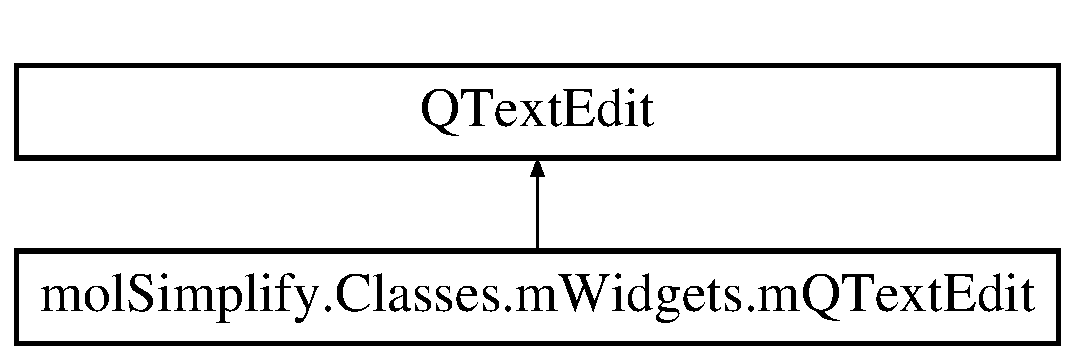
\includegraphics[height=2.000000cm]{classmolSimplify_1_1Classes_1_1mWidgets_1_1mQTextEdit}
\end{center}
\end{figure}
\subsection*{Public Member Functions}
\begin{DoxyCompactItemize}
\item 
def \hyperlink{classmolSimplify_1_1Classes_1_1mWidgets_1_1mQTextEdit_a5d753f694cc085bbdd6422bae4992abb}{\+\_\+\+\_\+init\+\_\+\+\_\+} (self, txt, align, fontsize)
\end{DoxyCompactItemize}


\subsection{Detailed Description}
G\+UI editor class. 

\subsection{Constructor \& Destructor Documentation}
\mbox{\Hypertarget{classmolSimplify_1_1Classes_1_1mWidgets_1_1mQTextEdit_a5d753f694cc085bbdd6422bae4992abb}\label{classmolSimplify_1_1Classes_1_1mWidgets_1_1mQTextEdit_a5d753f694cc085bbdd6422bae4992abb}} 
\index{mol\+Simplify\+::\+Classes\+::m\+Widgets\+::m\+Q\+Text\+Edit@{mol\+Simplify\+::\+Classes\+::m\+Widgets\+::m\+Q\+Text\+Edit}!\+\_\+\+\_\+init\+\_\+\+\_\+@{\+\_\+\+\_\+init\+\_\+\+\_\+}}
\index{\+\_\+\+\_\+init\+\_\+\+\_\+@{\+\_\+\+\_\+init\+\_\+\+\_\+}!mol\+Simplify\+::\+Classes\+::m\+Widgets\+::m\+Q\+Text\+Edit@{mol\+Simplify\+::\+Classes\+::m\+Widgets\+::m\+Q\+Text\+Edit}}
\subsubsection{\texorpdfstring{\+\_\+\+\_\+init\+\_\+\+\_\+()}{\_\_init\_\_()}}
{\footnotesize\ttfamily def mol\+Simplify.\+Classes.\+m\+Widgets.\+m\+Q\+Text\+Edit.\+\_\+\+\_\+init\+\_\+\+\_\+ (\begin{DoxyParamCaption}\item[{}]{self,  }\item[{}]{txt,  }\item[{}]{align,  }\item[{}]{fontsize }\end{DoxyParamCaption})}



The documentation for this class was generated from the following file\+:\begin{DoxyCompactItemize}
\item 
Classes/\hyperlink{mWidgets_8py}{m\+Widgets.\+py}\end{DoxyCompactItemize}

\hypertarget{classmolSimplify_1_1Classes_1_1mWidgets_1_1mSvgWidget}{}\section{mol\+Simplify.\+Classes.\+m\+Widgets.\+m\+Svg\+Widget Class Reference}
\label{classmolSimplify_1_1Classes_1_1mWidgets_1_1mSvgWidget}\index{mol\+Simplify.\+Classes.\+m\+Widgets.\+m\+Svg\+Widget@{mol\+Simplify.\+Classes.\+m\+Widgets.\+m\+Svg\+Widget}}


G\+UI svg widget class.  


Inheritance diagram for mol\+Simplify.\+Classes.\+m\+Widgets.\+m\+Svg\+Widget\+:\begin{figure}[H]
\begin{center}
\leavevmode
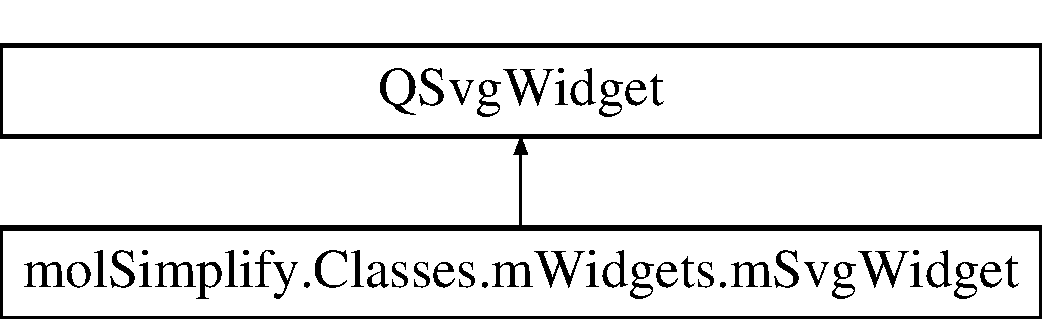
\includegraphics[height=2.000000cm]{classmolSimplify_1_1Classes_1_1mWidgets_1_1mSvgWidget}
\end{center}
\end{figure}
\subsection*{Public Member Functions}
\begin{DoxyCompactItemize}
\item 
def \hyperlink{classmolSimplify_1_1Classes_1_1mWidgets_1_1mSvgWidget_aa11201d67c84576d929ede296b2a447e}{\+\_\+\+\_\+init\+\_\+\+\_\+} (self, svgpath)
\end{DoxyCompactItemize}


\subsection{Detailed Description}
G\+UI svg widget class. 

\subsection{Constructor \& Destructor Documentation}
\mbox{\Hypertarget{classmolSimplify_1_1Classes_1_1mWidgets_1_1mSvgWidget_aa11201d67c84576d929ede296b2a447e}\label{classmolSimplify_1_1Classes_1_1mWidgets_1_1mSvgWidget_aa11201d67c84576d929ede296b2a447e}} 
\index{mol\+Simplify\+::\+Classes\+::m\+Widgets\+::m\+Svg\+Widget@{mol\+Simplify\+::\+Classes\+::m\+Widgets\+::m\+Svg\+Widget}!\+\_\+\+\_\+init\+\_\+\+\_\+@{\+\_\+\+\_\+init\+\_\+\+\_\+}}
\index{\+\_\+\+\_\+init\+\_\+\+\_\+@{\+\_\+\+\_\+init\+\_\+\+\_\+}!mol\+Simplify\+::\+Classes\+::m\+Widgets\+::m\+Svg\+Widget@{mol\+Simplify\+::\+Classes\+::m\+Widgets\+::m\+Svg\+Widget}}
\subsubsection{\texorpdfstring{\+\_\+\+\_\+init\+\_\+\+\_\+()}{\_\_init\_\_()}}
{\footnotesize\ttfamily def mol\+Simplify.\+Classes.\+m\+Widgets.\+m\+Svg\+Widget.\+\_\+\+\_\+init\+\_\+\+\_\+ (\begin{DoxyParamCaption}\item[{}]{self,  }\item[{}]{svgpath }\end{DoxyParamCaption})}



The documentation for this class was generated from the following file\+:\begin{DoxyCompactItemize}
\item 
Classes/\hyperlink{mWidgets_8py}{m\+Widgets.\+py}\end{DoxyCompactItemize}

\hypertarget{classmolSimplify_1_1Classes_1_1mWidgets_1_1qBoxFolder}{}\section{mol\+Simplify.\+Classes.\+m\+Widgets.\+q\+Box\+Folder Class Reference}
\label{classmolSimplify_1_1Classes_1_1mWidgets_1_1qBoxFolder}\index{mol\+Simplify.\+Classes.\+m\+Widgets.\+q\+Box\+Folder@{mol\+Simplify.\+Classes.\+m\+Widgets.\+q\+Box\+Folder}}


G\+UI box folder class.  


Inheritance diagram for mol\+Simplify.\+Classes.\+m\+Widgets.\+q\+Box\+Folder\+:\begin{figure}[H]
\begin{center}
\leavevmode
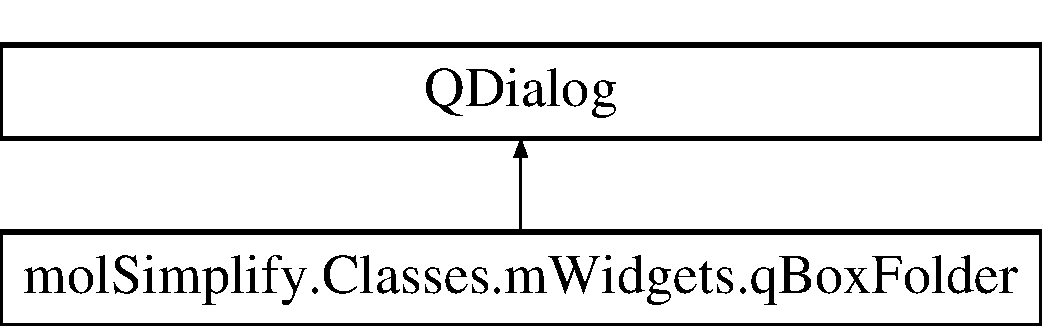
\includegraphics[height=2.000000cm]{classmolSimplify_1_1Classes_1_1mWidgets_1_1qBoxFolder}
\end{center}
\end{figure}
\subsection*{Public Member Functions}
\begin{DoxyCompactItemize}
\item 
def \hyperlink{classmolSimplify_1_1Classes_1_1mWidgets_1_1qBoxFolder_a619142b92e22bd580fe101c12b86131d}{\+\_\+\+\_\+init\+\_\+\+\_\+} (self, window, toptxt, txt)
\item 
def \hyperlink{classmolSimplify_1_1Classes_1_1mWidgets_1_1qBoxFolder_a42b4841cdd10db50295cfb41dcbd4b45}{getaction} (self)
\end{DoxyCompactItemize}
\subsection*{Public Attributes}
\begin{DoxyCompactItemize}
\item 
\hyperlink{classmolSimplify_1_1Classes_1_1mWidgets_1_1qBoxFolder_ae361b015d43881534ea206e92332ded2}{msg\+Box}
\end{DoxyCompactItemize}


\subsection{Detailed Description}
G\+UI box folder class. 

\subsection{Constructor \& Destructor Documentation}
\mbox{\Hypertarget{classmolSimplify_1_1Classes_1_1mWidgets_1_1qBoxFolder_a619142b92e22bd580fe101c12b86131d}\label{classmolSimplify_1_1Classes_1_1mWidgets_1_1qBoxFolder_a619142b92e22bd580fe101c12b86131d}} 
\index{mol\+Simplify\+::\+Classes\+::m\+Widgets\+::q\+Box\+Folder@{mol\+Simplify\+::\+Classes\+::m\+Widgets\+::q\+Box\+Folder}!\+\_\+\+\_\+init\+\_\+\+\_\+@{\+\_\+\+\_\+init\+\_\+\+\_\+}}
\index{\+\_\+\+\_\+init\+\_\+\+\_\+@{\+\_\+\+\_\+init\+\_\+\+\_\+}!mol\+Simplify\+::\+Classes\+::m\+Widgets\+::q\+Box\+Folder@{mol\+Simplify\+::\+Classes\+::m\+Widgets\+::q\+Box\+Folder}}
\subsubsection{\texorpdfstring{\+\_\+\+\_\+init\+\_\+\+\_\+()}{\_\_init\_\_()}}
{\footnotesize\ttfamily def mol\+Simplify.\+Classes.\+m\+Widgets.\+q\+Box\+Folder.\+\_\+\+\_\+init\+\_\+\+\_\+ (\begin{DoxyParamCaption}\item[{}]{self,  }\item[{}]{window,  }\item[{}]{toptxt,  }\item[{}]{txt }\end{DoxyParamCaption})}



\subsection{Member Function Documentation}
\mbox{\Hypertarget{classmolSimplify_1_1Classes_1_1mWidgets_1_1qBoxFolder_a42b4841cdd10db50295cfb41dcbd4b45}\label{classmolSimplify_1_1Classes_1_1mWidgets_1_1qBoxFolder_a42b4841cdd10db50295cfb41dcbd4b45}} 
\index{mol\+Simplify\+::\+Classes\+::m\+Widgets\+::q\+Box\+Folder@{mol\+Simplify\+::\+Classes\+::m\+Widgets\+::q\+Box\+Folder}!getaction@{getaction}}
\index{getaction@{getaction}!mol\+Simplify\+::\+Classes\+::m\+Widgets\+::q\+Box\+Folder@{mol\+Simplify\+::\+Classes\+::m\+Widgets\+::q\+Box\+Folder}}
\subsubsection{\texorpdfstring{getaction()}{getaction()}}
{\footnotesize\ttfamily def mol\+Simplify.\+Classes.\+m\+Widgets.\+q\+Box\+Folder.\+getaction (\begin{DoxyParamCaption}\item[{}]{self }\end{DoxyParamCaption})}



\subsection{Member Data Documentation}
\mbox{\Hypertarget{classmolSimplify_1_1Classes_1_1mWidgets_1_1qBoxFolder_ae361b015d43881534ea206e92332ded2}\label{classmolSimplify_1_1Classes_1_1mWidgets_1_1qBoxFolder_ae361b015d43881534ea206e92332ded2}} 
\index{mol\+Simplify\+::\+Classes\+::m\+Widgets\+::q\+Box\+Folder@{mol\+Simplify\+::\+Classes\+::m\+Widgets\+::q\+Box\+Folder}!msg\+Box@{msg\+Box}}
\index{msg\+Box@{msg\+Box}!mol\+Simplify\+::\+Classes\+::m\+Widgets\+::q\+Box\+Folder@{mol\+Simplify\+::\+Classes\+::m\+Widgets\+::q\+Box\+Folder}}
\subsubsection{\texorpdfstring{msg\+Box}{msgBox}}
{\footnotesize\ttfamily mol\+Simplify.\+Classes.\+m\+Widgets.\+q\+Box\+Folder.\+msg\+Box}



The documentation for this class was generated from the following file\+:\begin{DoxyCompactItemize}
\item 
Classes/\hyperlink{mWidgets_8py}{m\+Widgets.\+py}\end{DoxyCompactItemize}

\hypertarget{classmolSimplify_1_1Classes_1_1rundiag_1_1run__diag}{}\section{mol\+Simplify.\+Classes.\+rundiag.\+run\+\_\+diag Class Reference}
\label{classmolSimplify_1_1Classes_1_1rundiag_1_1run__diag}\index{mol\+Simplify.\+Classes.\+rundiag.\+run\+\_\+diag@{mol\+Simplify.\+Classes.\+rundiag.\+run\+\_\+diag}}


Class of run diagnostic information to automated decision making and property prediction.  


\subsection*{Public Member Functions}
\begin{DoxyCompactItemize}
\item 
def \hyperlink{classmolSimplify_1_1Classes_1_1rundiag_1_1run__diag_a991e53c0bab164d1b921960f19597890}{\+\_\+\+\_\+init\+\_\+\+\_\+} (self)
\begin{DoxyCompactList}\small\item\em Constructor. \end{DoxyCompactList}\item 
def \hyperlink{classmolSimplify_1_1Classes_1_1rundiag_1_1run__diag_a659afacfb2e4f24e08ee965d9b93a7e2}{set\+\_\+sanity} (self, \hyperlink{classmolSimplify_1_1Classes_1_1rundiag_1_1run__diag_a0ef07fdeafae0c40968a4b2cffc5ca33}{sanity}, min\+\_\+distance)
\begin{DoxyCompactList}\small\item\em class methods needed to populate \#\#\# \end{DoxyCompactList}\item 
def \hyperlink{classmolSimplify_1_1Classes_1_1rundiag_1_1run__diag_a065d2729214e5d3af49f9435a585cb11}{set\+\_\+\+A\+NN} (self, \hyperlink{classmolSimplify_1_1Classes_1_1rundiag_1_1run__diag_ab77602b8de86bb282c07b2243f134590}{A\+N\+N\+\_\+flag}, \hyperlink{classmolSimplify_1_1Classes_1_1rundiag_1_1run__diag_a92f327be2e53727b00848e18f8427af9}{A\+N\+N\+\_\+reason}=False, A\+N\+N\+\_\+dict=False)
\item 
def \hyperlink{classmolSimplify_1_1Classes_1_1rundiag_1_1run__diag_aafd5fdd0e5de8e0d1caf2de4ee328599}{set\+\_\+dict\+\_\+bl} (self, dict\+\_\+bl)
\item 
def \hyperlink{classmolSimplify_1_1Classes_1_1rundiag_1_1run__diag_a3ad834b2a3202758c1801986cc9c77e2}{set\+\_\+mol} (self, \hyperlink{classmolSimplify_1_1Classes_1_1rundiag_1_1run__diag_a403fc5dcab3e50c5fec055bf9bbf6fb0}{mol})
\item 
def \hyperlink{classmolSimplify_1_1Classes_1_1rundiag_1_1run__diag_a68d29a7ca70f2138da2740feaee1c7cd}{write\+\_\+report} (self, path)
\begin{DoxyCompactList}\small\item\em class methods needed to report \#\#\#\# \end{DoxyCompactList}\end{DoxyCompactItemize}
\subsection*{Public Attributes}
\begin{DoxyCompactItemize}
\item 
\hyperlink{classmolSimplify_1_1Classes_1_1rundiag_1_1run__diag_a589e3d95a6d3b459b9d691f1489710ef}{sanity\+\_\+is\+\_\+set}
\item 
\hyperlink{classmolSimplify_1_1Classes_1_1rundiag_1_1run__diag_acbc5d5a67868d62ae0f3d9487816476e}{A\+N\+N\+\_\+is\+\_\+set}
\item 
\hyperlink{classmolSimplify_1_1Classes_1_1rundiag_1_1run__diag_a9169c98f4a082e5ba9a611dcd7f14dfe}{bl\+\_\+is\+\_\+set}
\item 
\hyperlink{classmolSimplify_1_1Classes_1_1rundiag_1_1run__diag_ac2ff49e58753e9a38fdce364e780c4e9}{mol\+\_\+is\+\_\+set}
\item 
\hyperlink{classmolSimplify_1_1Classes_1_1rundiag_1_1run__diag_a0ef07fdeafae0c40968a4b2cffc5ca33}{sanity}
\item 
\hyperlink{classmolSimplify_1_1Classes_1_1rundiag_1_1run__diag_a52afc50b5c44a45ae06443998f700691}{min\+\_\+dist}
\item 
\hyperlink{classmolSimplify_1_1Classes_1_1rundiag_1_1run__diag_ab77602b8de86bb282c07b2243f134590}{A\+N\+N\+\_\+flag}
\item 
\hyperlink{classmolSimplify_1_1Classes_1_1rundiag_1_1run__diag_a92f327be2e53727b00848e18f8427af9}{A\+N\+N\+\_\+reason}
\item 
\hyperlink{classmolSimplify_1_1Classes_1_1rundiag_1_1run__diag_a2188d3f122764860e545bbe18472255a}{A\+N\+N\+\_\+attributes}
\item 
\hyperlink{classmolSimplify_1_1Classes_1_1rundiag_1_1run__diag_ae47d840dc466b06e8d0d5495622acc08}{dict\+\_\+bondl}
\item 
\hyperlink{classmolSimplify_1_1Classes_1_1rundiag_1_1run__diag_a403fc5dcab3e50c5fec055bf9bbf6fb0}{mol}
\end{DoxyCompactItemize}


\subsection{Detailed Description}
Class of run diagnostic information to automated decision making and property prediction. 

\subsection{Constructor \& Destructor Documentation}
\mbox{\Hypertarget{classmolSimplify_1_1Classes_1_1rundiag_1_1run__diag_a991e53c0bab164d1b921960f19597890}\label{classmolSimplify_1_1Classes_1_1rundiag_1_1run__diag_a991e53c0bab164d1b921960f19597890}} 
\index{mol\+Simplify\+::\+Classes\+::rundiag\+::run\+\_\+diag@{mol\+Simplify\+::\+Classes\+::rundiag\+::run\+\_\+diag}!\+\_\+\+\_\+init\+\_\+\+\_\+@{\+\_\+\+\_\+init\+\_\+\+\_\+}}
\index{\+\_\+\+\_\+init\+\_\+\+\_\+@{\+\_\+\+\_\+init\+\_\+\+\_\+}!mol\+Simplify\+::\+Classes\+::rundiag\+::run\+\_\+diag@{mol\+Simplify\+::\+Classes\+::rundiag\+::run\+\_\+diag}}
\subsubsection{\texorpdfstring{\+\_\+\+\_\+init\+\_\+\+\_\+()}{\_\_init\_\_()}}
{\footnotesize\ttfamily def mol\+Simplify.\+Classes.\+rundiag.\+run\+\_\+diag.\+\_\+\+\_\+init\+\_\+\+\_\+ (\begin{DoxyParamCaption}\item[{}]{self }\end{DoxyParamCaption})}



Constructor. 


\begin{DoxyParams}{Parameters}
{\em self} & The object pointer \\
\hline
\end{DoxyParams}


\subsection{Member Function Documentation}
\mbox{\Hypertarget{classmolSimplify_1_1Classes_1_1rundiag_1_1run__diag_a065d2729214e5d3af49f9435a585cb11}\label{classmolSimplify_1_1Classes_1_1rundiag_1_1run__diag_a065d2729214e5d3af49f9435a585cb11}} 
\index{mol\+Simplify\+::\+Classes\+::rundiag\+::run\+\_\+diag@{mol\+Simplify\+::\+Classes\+::rundiag\+::run\+\_\+diag}!set\+\_\+\+A\+NN@{set\+\_\+\+A\+NN}}
\index{set\+\_\+\+A\+NN@{set\+\_\+\+A\+NN}!mol\+Simplify\+::\+Classes\+::rundiag\+::run\+\_\+diag@{mol\+Simplify\+::\+Classes\+::rundiag\+::run\+\_\+diag}}
\subsubsection{\texorpdfstring{set\+\_\+\+A\+N\+N()}{set\_ANN()}}
{\footnotesize\ttfamily def mol\+Simplify.\+Classes.\+rundiag.\+run\+\_\+diag.\+set\+\_\+\+A\+NN (\begin{DoxyParamCaption}\item[{}]{self,  }\item[{}]{A\+N\+N\+\_\+flag,  }\item[{}]{A\+N\+N\+\_\+reason = {\ttfamily False},  }\item[{}]{A\+N\+N\+\_\+dict = {\ttfamily False} }\end{DoxyParamCaption})}

\mbox{\Hypertarget{classmolSimplify_1_1Classes_1_1rundiag_1_1run__diag_aafd5fdd0e5de8e0d1caf2de4ee328599}\label{classmolSimplify_1_1Classes_1_1rundiag_1_1run__diag_aafd5fdd0e5de8e0d1caf2de4ee328599}} 
\index{mol\+Simplify\+::\+Classes\+::rundiag\+::run\+\_\+diag@{mol\+Simplify\+::\+Classes\+::rundiag\+::run\+\_\+diag}!set\+\_\+dict\+\_\+bl@{set\+\_\+dict\+\_\+bl}}
\index{set\+\_\+dict\+\_\+bl@{set\+\_\+dict\+\_\+bl}!mol\+Simplify\+::\+Classes\+::rundiag\+::run\+\_\+diag@{mol\+Simplify\+::\+Classes\+::rundiag\+::run\+\_\+diag}}
\subsubsection{\texorpdfstring{set\+\_\+dict\+\_\+bl()}{set\_dict\_bl()}}
{\footnotesize\ttfamily def mol\+Simplify.\+Classes.\+rundiag.\+run\+\_\+diag.\+set\+\_\+dict\+\_\+bl (\begin{DoxyParamCaption}\item[{}]{self,  }\item[{}]{dict\+\_\+bl }\end{DoxyParamCaption})}

\mbox{\Hypertarget{classmolSimplify_1_1Classes_1_1rundiag_1_1run__diag_a3ad834b2a3202758c1801986cc9c77e2}\label{classmolSimplify_1_1Classes_1_1rundiag_1_1run__diag_a3ad834b2a3202758c1801986cc9c77e2}} 
\index{mol\+Simplify\+::\+Classes\+::rundiag\+::run\+\_\+diag@{mol\+Simplify\+::\+Classes\+::rundiag\+::run\+\_\+diag}!set\+\_\+mol@{set\+\_\+mol}}
\index{set\+\_\+mol@{set\+\_\+mol}!mol\+Simplify\+::\+Classes\+::rundiag\+::run\+\_\+diag@{mol\+Simplify\+::\+Classes\+::rundiag\+::run\+\_\+diag}}
\subsubsection{\texorpdfstring{set\+\_\+mol()}{set\_mol()}}
{\footnotesize\ttfamily def mol\+Simplify.\+Classes.\+rundiag.\+run\+\_\+diag.\+set\+\_\+mol (\begin{DoxyParamCaption}\item[{}]{self,  }\item[{}]{mol }\end{DoxyParamCaption})}

\mbox{\Hypertarget{classmolSimplify_1_1Classes_1_1rundiag_1_1run__diag_a659afacfb2e4f24e08ee965d9b93a7e2}\label{classmolSimplify_1_1Classes_1_1rundiag_1_1run__diag_a659afacfb2e4f24e08ee965d9b93a7e2}} 
\index{mol\+Simplify\+::\+Classes\+::rundiag\+::run\+\_\+diag@{mol\+Simplify\+::\+Classes\+::rundiag\+::run\+\_\+diag}!set\+\_\+sanity@{set\+\_\+sanity}}
\index{set\+\_\+sanity@{set\+\_\+sanity}!mol\+Simplify\+::\+Classes\+::rundiag\+::run\+\_\+diag@{mol\+Simplify\+::\+Classes\+::rundiag\+::run\+\_\+diag}}
\subsubsection{\texorpdfstring{set\+\_\+sanity()}{set\_sanity()}}
{\footnotesize\ttfamily def mol\+Simplify.\+Classes.\+rundiag.\+run\+\_\+diag.\+set\+\_\+sanity (\begin{DoxyParamCaption}\item[{}]{self,  }\item[{}]{sanity,  }\item[{}]{min\+\_\+distance }\end{DoxyParamCaption})}



class methods needed to populate \#\#\# 

\mbox{\Hypertarget{classmolSimplify_1_1Classes_1_1rundiag_1_1run__diag_a68d29a7ca70f2138da2740feaee1c7cd}\label{classmolSimplify_1_1Classes_1_1rundiag_1_1run__diag_a68d29a7ca70f2138da2740feaee1c7cd}} 
\index{mol\+Simplify\+::\+Classes\+::rundiag\+::run\+\_\+diag@{mol\+Simplify\+::\+Classes\+::rundiag\+::run\+\_\+diag}!write\+\_\+report@{write\+\_\+report}}
\index{write\+\_\+report@{write\+\_\+report}!mol\+Simplify\+::\+Classes\+::rundiag\+::run\+\_\+diag@{mol\+Simplify\+::\+Classes\+::rundiag\+::run\+\_\+diag}}
\subsubsection{\texorpdfstring{write\+\_\+report()}{write\_report()}}
{\footnotesize\ttfamily def mol\+Simplify.\+Classes.\+rundiag.\+run\+\_\+diag.\+write\+\_\+report (\begin{DoxyParamCaption}\item[{}]{self,  }\item[{}]{path }\end{DoxyParamCaption})}



class methods needed to report \#\#\#\# 



\subsection{Member Data Documentation}
\mbox{\Hypertarget{classmolSimplify_1_1Classes_1_1rundiag_1_1run__diag_a2188d3f122764860e545bbe18472255a}\label{classmolSimplify_1_1Classes_1_1rundiag_1_1run__diag_a2188d3f122764860e545bbe18472255a}} 
\index{mol\+Simplify\+::\+Classes\+::rundiag\+::run\+\_\+diag@{mol\+Simplify\+::\+Classes\+::rundiag\+::run\+\_\+diag}!A\+N\+N\+\_\+attributes@{A\+N\+N\+\_\+attributes}}
\index{A\+N\+N\+\_\+attributes@{A\+N\+N\+\_\+attributes}!mol\+Simplify\+::\+Classes\+::rundiag\+::run\+\_\+diag@{mol\+Simplify\+::\+Classes\+::rundiag\+::run\+\_\+diag}}
\subsubsection{\texorpdfstring{A\+N\+N\+\_\+attributes}{ANN\_attributes}}
{\footnotesize\ttfamily mol\+Simplify.\+Classes.\+rundiag.\+run\+\_\+diag.\+A\+N\+N\+\_\+attributes}

\mbox{\Hypertarget{classmolSimplify_1_1Classes_1_1rundiag_1_1run__diag_ab77602b8de86bb282c07b2243f134590}\label{classmolSimplify_1_1Classes_1_1rundiag_1_1run__diag_ab77602b8de86bb282c07b2243f134590}} 
\index{mol\+Simplify\+::\+Classes\+::rundiag\+::run\+\_\+diag@{mol\+Simplify\+::\+Classes\+::rundiag\+::run\+\_\+diag}!A\+N\+N\+\_\+flag@{A\+N\+N\+\_\+flag}}
\index{A\+N\+N\+\_\+flag@{A\+N\+N\+\_\+flag}!mol\+Simplify\+::\+Classes\+::rundiag\+::run\+\_\+diag@{mol\+Simplify\+::\+Classes\+::rundiag\+::run\+\_\+diag}}
\subsubsection{\texorpdfstring{A\+N\+N\+\_\+flag}{ANN\_flag}}
{\footnotesize\ttfamily mol\+Simplify.\+Classes.\+rundiag.\+run\+\_\+diag.\+A\+N\+N\+\_\+flag}

\mbox{\Hypertarget{classmolSimplify_1_1Classes_1_1rundiag_1_1run__diag_acbc5d5a67868d62ae0f3d9487816476e}\label{classmolSimplify_1_1Classes_1_1rundiag_1_1run__diag_acbc5d5a67868d62ae0f3d9487816476e}} 
\index{mol\+Simplify\+::\+Classes\+::rundiag\+::run\+\_\+diag@{mol\+Simplify\+::\+Classes\+::rundiag\+::run\+\_\+diag}!A\+N\+N\+\_\+is\+\_\+set@{A\+N\+N\+\_\+is\+\_\+set}}
\index{A\+N\+N\+\_\+is\+\_\+set@{A\+N\+N\+\_\+is\+\_\+set}!mol\+Simplify\+::\+Classes\+::rundiag\+::run\+\_\+diag@{mol\+Simplify\+::\+Classes\+::rundiag\+::run\+\_\+diag}}
\subsubsection{\texorpdfstring{A\+N\+N\+\_\+is\+\_\+set}{ANN\_is\_set}}
{\footnotesize\ttfamily mol\+Simplify.\+Classes.\+rundiag.\+run\+\_\+diag.\+A\+N\+N\+\_\+is\+\_\+set}

\mbox{\Hypertarget{classmolSimplify_1_1Classes_1_1rundiag_1_1run__diag_a92f327be2e53727b00848e18f8427af9}\label{classmolSimplify_1_1Classes_1_1rundiag_1_1run__diag_a92f327be2e53727b00848e18f8427af9}} 
\index{mol\+Simplify\+::\+Classes\+::rundiag\+::run\+\_\+diag@{mol\+Simplify\+::\+Classes\+::rundiag\+::run\+\_\+diag}!A\+N\+N\+\_\+reason@{A\+N\+N\+\_\+reason}}
\index{A\+N\+N\+\_\+reason@{A\+N\+N\+\_\+reason}!mol\+Simplify\+::\+Classes\+::rundiag\+::run\+\_\+diag@{mol\+Simplify\+::\+Classes\+::rundiag\+::run\+\_\+diag}}
\subsubsection{\texorpdfstring{A\+N\+N\+\_\+reason}{ANN\_reason}}
{\footnotesize\ttfamily mol\+Simplify.\+Classes.\+rundiag.\+run\+\_\+diag.\+A\+N\+N\+\_\+reason}

\mbox{\Hypertarget{classmolSimplify_1_1Classes_1_1rundiag_1_1run__diag_a9169c98f4a082e5ba9a611dcd7f14dfe}\label{classmolSimplify_1_1Classes_1_1rundiag_1_1run__diag_a9169c98f4a082e5ba9a611dcd7f14dfe}} 
\index{mol\+Simplify\+::\+Classes\+::rundiag\+::run\+\_\+diag@{mol\+Simplify\+::\+Classes\+::rundiag\+::run\+\_\+diag}!bl\+\_\+is\+\_\+set@{bl\+\_\+is\+\_\+set}}
\index{bl\+\_\+is\+\_\+set@{bl\+\_\+is\+\_\+set}!mol\+Simplify\+::\+Classes\+::rundiag\+::run\+\_\+diag@{mol\+Simplify\+::\+Classes\+::rundiag\+::run\+\_\+diag}}
\subsubsection{\texorpdfstring{bl\+\_\+is\+\_\+set}{bl\_is\_set}}
{\footnotesize\ttfamily mol\+Simplify.\+Classes.\+rundiag.\+run\+\_\+diag.\+bl\+\_\+is\+\_\+set}

\mbox{\Hypertarget{classmolSimplify_1_1Classes_1_1rundiag_1_1run__diag_ae47d840dc466b06e8d0d5495622acc08}\label{classmolSimplify_1_1Classes_1_1rundiag_1_1run__diag_ae47d840dc466b06e8d0d5495622acc08}} 
\index{mol\+Simplify\+::\+Classes\+::rundiag\+::run\+\_\+diag@{mol\+Simplify\+::\+Classes\+::rundiag\+::run\+\_\+diag}!dict\+\_\+bondl@{dict\+\_\+bondl}}
\index{dict\+\_\+bondl@{dict\+\_\+bondl}!mol\+Simplify\+::\+Classes\+::rundiag\+::run\+\_\+diag@{mol\+Simplify\+::\+Classes\+::rundiag\+::run\+\_\+diag}}
\subsubsection{\texorpdfstring{dict\+\_\+bondl}{dict\_bondl}}
{\footnotesize\ttfamily mol\+Simplify.\+Classes.\+rundiag.\+run\+\_\+diag.\+dict\+\_\+bondl}

\mbox{\Hypertarget{classmolSimplify_1_1Classes_1_1rundiag_1_1run__diag_a52afc50b5c44a45ae06443998f700691}\label{classmolSimplify_1_1Classes_1_1rundiag_1_1run__diag_a52afc50b5c44a45ae06443998f700691}} 
\index{mol\+Simplify\+::\+Classes\+::rundiag\+::run\+\_\+diag@{mol\+Simplify\+::\+Classes\+::rundiag\+::run\+\_\+diag}!min\+\_\+dist@{min\+\_\+dist}}
\index{min\+\_\+dist@{min\+\_\+dist}!mol\+Simplify\+::\+Classes\+::rundiag\+::run\+\_\+diag@{mol\+Simplify\+::\+Classes\+::rundiag\+::run\+\_\+diag}}
\subsubsection{\texorpdfstring{min\+\_\+dist}{min\_dist}}
{\footnotesize\ttfamily mol\+Simplify.\+Classes.\+rundiag.\+run\+\_\+diag.\+min\+\_\+dist}

\mbox{\Hypertarget{classmolSimplify_1_1Classes_1_1rundiag_1_1run__diag_a403fc5dcab3e50c5fec055bf9bbf6fb0}\label{classmolSimplify_1_1Classes_1_1rundiag_1_1run__diag_a403fc5dcab3e50c5fec055bf9bbf6fb0}} 
\index{mol\+Simplify\+::\+Classes\+::rundiag\+::run\+\_\+diag@{mol\+Simplify\+::\+Classes\+::rundiag\+::run\+\_\+diag}!mol@{mol}}
\index{mol@{mol}!mol\+Simplify\+::\+Classes\+::rundiag\+::run\+\_\+diag@{mol\+Simplify\+::\+Classes\+::rundiag\+::run\+\_\+diag}}
\subsubsection{\texorpdfstring{mol}{mol}}
{\footnotesize\ttfamily mol\+Simplify.\+Classes.\+rundiag.\+run\+\_\+diag.\+mol}

\mbox{\Hypertarget{classmolSimplify_1_1Classes_1_1rundiag_1_1run__diag_ac2ff49e58753e9a38fdce364e780c4e9}\label{classmolSimplify_1_1Classes_1_1rundiag_1_1run__diag_ac2ff49e58753e9a38fdce364e780c4e9}} 
\index{mol\+Simplify\+::\+Classes\+::rundiag\+::run\+\_\+diag@{mol\+Simplify\+::\+Classes\+::rundiag\+::run\+\_\+diag}!mol\+\_\+is\+\_\+set@{mol\+\_\+is\+\_\+set}}
\index{mol\+\_\+is\+\_\+set@{mol\+\_\+is\+\_\+set}!mol\+Simplify\+::\+Classes\+::rundiag\+::run\+\_\+diag@{mol\+Simplify\+::\+Classes\+::rundiag\+::run\+\_\+diag}}
\subsubsection{\texorpdfstring{mol\+\_\+is\+\_\+set}{mol\_is\_set}}
{\footnotesize\ttfamily mol\+Simplify.\+Classes.\+rundiag.\+run\+\_\+diag.\+mol\+\_\+is\+\_\+set}

\mbox{\Hypertarget{classmolSimplify_1_1Classes_1_1rundiag_1_1run__diag_a0ef07fdeafae0c40968a4b2cffc5ca33}\label{classmolSimplify_1_1Classes_1_1rundiag_1_1run__diag_a0ef07fdeafae0c40968a4b2cffc5ca33}} 
\index{mol\+Simplify\+::\+Classes\+::rundiag\+::run\+\_\+diag@{mol\+Simplify\+::\+Classes\+::rundiag\+::run\+\_\+diag}!sanity@{sanity}}
\index{sanity@{sanity}!mol\+Simplify\+::\+Classes\+::rundiag\+::run\+\_\+diag@{mol\+Simplify\+::\+Classes\+::rundiag\+::run\+\_\+diag}}
\subsubsection{\texorpdfstring{sanity}{sanity}}
{\footnotesize\ttfamily mol\+Simplify.\+Classes.\+rundiag.\+run\+\_\+diag.\+sanity}

\mbox{\Hypertarget{classmolSimplify_1_1Classes_1_1rundiag_1_1run__diag_a589e3d95a6d3b459b9d691f1489710ef}\label{classmolSimplify_1_1Classes_1_1rundiag_1_1run__diag_a589e3d95a6d3b459b9d691f1489710ef}} 
\index{mol\+Simplify\+::\+Classes\+::rundiag\+::run\+\_\+diag@{mol\+Simplify\+::\+Classes\+::rundiag\+::run\+\_\+diag}!sanity\+\_\+is\+\_\+set@{sanity\+\_\+is\+\_\+set}}
\index{sanity\+\_\+is\+\_\+set@{sanity\+\_\+is\+\_\+set}!mol\+Simplify\+::\+Classes\+::rundiag\+::run\+\_\+diag@{mol\+Simplify\+::\+Classes\+::rundiag\+::run\+\_\+diag}}
\subsubsection{\texorpdfstring{sanity\+\_\+is\+\_\+set}{sanity\_is\_set}}
{\footnotesize\ttfamily mol\+Simplify.\+Classes.\+rundiag.\+run\+\_\+diag.\+sanity\+\_\+is\+\_\+set}



The documentation for this class was generated from the following file\+:\begin{DoxyCompactItemize}
\item 
Classes/\hyperlink{rundiag_8py}{rundiag.\+py}\end{DoxyCompactItemize}

\chapter{File Documentation}
\hypertarget{____init_____8py}{}\section{\+\_\+\+\_\+init\+\_\+\+\_\+.\+py File Reference}
\label{____init_____8py}\index{\+\_\+\+\_\+init\+\_\+\+\_\+.\+py@{\+\_\+\+\_\+init\+\_\+\+\_\+.\+py}}
\subsection*{Namespaces}
\begin{DoxyCompactItemize}
\item 
 \hyperlink{namespacemolSimplify}{mol\+Simplify}
\end{DoxyCompactItemize}

\hypertarget{Classes_2____init_____8py}{}\section{Classes/\+\_\+\+\_\+init\+\_\+\+\_\+.py File Reference}
\label{Classes_2____init_____8py}\index{Classes/\+\_\+\+\_\+init\+\_\+\+\_\+.\+py@{Classes/\+\_\+\+\_\+init\+\_\+\+\_\+.\+py}}
\subsection*{Namespaces}
\begin{DoxyCompactItemize}
\item 
 \hyperlink{namespacemolSimplify_1_1Classes}{mol\+Simplify.\+Classes}
\end{DoxyCompactItemize}

\hypertarget{Informatics_2____init_____8py}{}\section{Informatics/\+\_\+\+\_\+init\+\_\+\+\_\+.py File Reference}
\label{Informatics_2____init_____8py}\index{Informatics/\+\_\+\+\_\+init\+\_\+\+\_\+.\+py@{Informatics/\+\_\+\+\_\+init\+\_\+\+\_\+.\+py}}
\subsection*{Namespaces}
\begin{DoxyCompactItemize}
\item 
 \hyperlink{namespacemolSimplify_1_1Informatics}{mol\+Simplify.\+Informatics}
\end{DoxyCompactItemize}

\hypertarget{python__nn_2____init_____8py}{}\section{python\+\_\+nn/\+\_\+\+\_\+init\+\_\+\+\_\+.py File Reference}
\label{python__nn_2____init_____8py}\index{python\+\_\+nn/\+\_\+\+\_\+init\+\_\+\+\_\+.\+py@{python\+\_\+nn/\+\_\+\+\_\+init\+\_\+\+\_\+.\+py}}
\subsection*{Namespaces}
\begin{DoxyCompactItemize}
\item 
 \hyperlink{namespacemolSimplify_1_1python__nn}{mol\+Simplify.\+python\+\_\+nn}
\end{DoxyCompactItemize}

\hypertarget{Scripts_2____init_____8py}{}\section{Scripts/\+\_\+\+\_\+init\+\_\+\+\_\+.py File Reference}
\label{Scripts_2____init_____8py}\index{Scripts/\+\_\+\+\_\+init\+\_\+\+\_\+.\+py@{Scripts/\+\_\+\+\_\+init\+\_\+\+\_\+.\+py}}
\subsection*{Namespaces}
\begin{DoxyCompactItemize}
\item 
 \hyperlink{namespacemolSimplify_1_1Scripts}{mol\+Simplify.\+Scripts}
\end{DoxyCompactItemize}

\hypertarget{____main_____8py}{}\section{\+\_\+\+\_\+main\+\_\+\+\_\+.\+py File Reference}
\label{____main_____8py}\index{\+\_\+\+\_\+main\+\_\+\+\_\+.\+py@{\+\_\+\+\_\+main\+\_\+\+\_\+.\+py}}


Gateway script to rest of program.  


\subsection*{Namespaces}
\begin{DoxyCompactItemize}
\item 
 \hyperlink{namespacemolSimplify_1_1____main____}{mol\+Simplify.\+\_\+\+\_\+main\+\_\+\+\_\+}
\end{DoxyCompactItemize}
\subsection*{Functions}
\begin{DoxyCompactItemize}
\item 
def \hyperlink{namespacemolSimplify_1_1____main_____ac0957a328f374bc27d3a68abb201da04}{mol\+Simplify.\+\_\+\+\_\+main\+\_\+\+\_\+.\+main} (args=None)
\begin{DoxyCompactList}\small\item\em Main function. \end{DoxyCompactList}\end{DoxyCompactItemize}
\subsection*{Variables}
\begin{DoxyCompactItemize}
\item 
\hyperlink{namespacemolSimplify_1_1____main_____a621b1b32cbc714e9bd9c879933b298e7}{mol\+Simplify.\+\_\+\+\_\+main\+\_\+\+\_\+.\+globs} = globalvars()
\item 
string \hyperlink{namespacemolSimplify_1_1____main_____aa347c2a18c98b8e1a03cda9ad0ce603e}{mol\+Simplify.\+\_\+\+\_\+main\+\_\+\+\_\+.\+Desc\+String\+\_\+basic} = \textquotesingle{}Welcome to mol\+Simplify. Only basic usage is described here.\textbackslash{}n\textquotesingle{}
\begin{DoxyCompactList}\small\item\em Basic help description string. \end{DoxyCompactList}\item 
string \hyperlink{namespacemolSimplify_1_1____main_____aaa9b13414a118be18409510c28ae5592}{mol\+Simplify.\+\_\+\+\_\+main\+\_\+\+\_\+.\+Desc\+String\+\_\+advanced} = \textquotesingle{}Printing advanced structure generation help.\textquotesingle{}
\begin{DoxyCompactList}\small\item\em Advanced help description string. \end{DoxyCompactList}\item 
string \hyperlink{namespacemolSimplify_1_1____main_____ace71611b150d4e92bdba41429d969875}{mol\+Simplify.\+\_\+\+\_\+main\+\_\+\+\_\+.\+Desc\+String\+\_\+slabgen} = \textquotesingle{}Printing slab builder help.\textquotesingle{}
\begin{DoxyCompactList}\small\item\em Slab builder help description string. \end{DoxyCompactList}\item 
string \hyperlink{namespacemolSimplify_1_1____main_____a44fcd92cdc8efbe8ae3581dfca56309c}{mol\+Simplify.\+\_\+\+\_\+main\+\_\+\+\_\+.\+Desc\+String\+\_\+chainb} = \textquotesingle{}Printing chain builder help.\textquotesingle{}
\begin{DoxyCompactList}\small\item\em Chain builder help description string. \end{DoxyCompactList}\item 
string \hyperlink{namespacemolSimplify_1_1____main_____a64212e9eeef243dd712d62c9dcfe1b34}{mol\+Simplify.\+\_\+\+\_\+main\+\_\+\+\_\+.\+Desc\+String\+\_\+autocorr} = \textquotesingle{}Printing automated correlation analysis help.\textquotesingle{}
\begin{DoxyCompactList}\small\item\em Automated correlation analysis description string. \end{DoxyCompactList}\item 
string \hyperlink{namespacemolSimplify_1_1____main_____a314d123a302fd3449d6d3dbb3cb27b8d}{mol\+Simplify.\+\_\+\+\_\+main\+\_\+\+\_\+.\+Desc\+String\+\_\+db} = \textquotesingle{}Printing database search help.\textquotesingle{}
\begin{DoxyCompactList}\small\item\em Database search help description string. \end{DoxyCompactList}\item 
string \hyperlink{namespacemolSimplify_1_1____main_____a1af5cd3b5f20025e5f4cb6ba23547f4f}{mol\+Simplify.\+\_\+\+\_\+main\+\_\+\+\_\+.\+Desc\+String\+\_\+inputgen} = \textquotesingle{}Printing quantum chemistry code input file generation help.\textquotesingle{}
\begin{DoxyCompactList}\small\item\em Input file generation help description string. \end{DoxyCompactList}\item 
string \hyperlink{namespacemolSimplify_1_1____main_____aa19f048e1fe6ed31edc79a7f0ab58982}{mol\+Simplify.\+\_\+\+\_\+main\+\_\+\+\_\+.\+Desc\+String\+\_\+postproc} = \textquotesingle{}Printing post-\/processing help.\textquotesingle{}
\begin{DoxyCompactList}\small\item\em Post-\/processing help description string. \end{DoxyCompactList}\item 
string \hyperlink{namespacemolSimplify_1_1____main_____a0a31dce622ac102581d73cd746598943}{mol\+Simplify.\+\_\+\+\_\+main\+\_\+\+\_\+.\+Desc\+String\+\_\+random} = \textquotesingle{}Printing random generation help.\textquotesingle{}
\begin{DoxyCompactList}\small\item\em Random generation help description string. \end{DoxyCompactList}\item 
string \hyperlink{namespacemolSimplify_1_1____main_____a66178dfe9e4007b22bd17c4e05c1fb00}{mol\+Simplify.\+\_\+\+\_\+main\+\_\+\+\_\+.\+Desc\+String\+\_\+binding} = \textquotesingle{}Printing binding species (second molecule) generation help.\textquotesingle{}
\begin{DoxyCompactList}\small\item\em Binding species placement help description string. \end{DoxyCompactList}\item 
string \hyperlink{namespacemolSimplify_1_1____main_____ab0c1aa41d4731fa63cb84b238351653f}{mol\+Simplify.\+\_\+\+\_\+main\+\_\+\+\_\+.\+Desc\+String\+\_\+tsgen} = \textquotesingle{}Printing transition state generation help.\textquotesingle{}
\begin{DoxyCompactList}\small\item\em Transition state generation help description string. \end{DoxyCompactList}\item 
string \hyperlink{namespacemolSimplify_1_1____main_____a496fa81c1389ea0f803ba654a8f34d13}{mol\+Simplify.\+\_\+\+\_\+main\+\_\+\+\_\+.\+Desc\+String\+\_\+customcore} = \textquotesingle{}Printing ligand replacement help.\textquotesingle{}
\begin{DoxyCompactList}\small\item\em Ligand replacement help description string. \end{DoxyCompactList}\item 
string \hyperlink{namespacemolSimplify_1_1____main_____a8f8d451490e4ae14efb40374fd9774f2}{mol\+Simplify.\+\_\+\+\_\+main\+\_\+\+\_\+.\+Desc\+String\+\_\+naming} = \textquotesingle{}Printing custom filename help.\textquotesingle{}
\begin{DoxyCompactList}\small\item\em Custom file naming help description string. \end{DoxyCompactList}\item 
bool \hyperlink{namespacemolSimplify_1_1____main_____a014c496de4ba28be70d30b5c0b77919b}{mol\+Simplify.\+\_\+\+\_\+main\+\_\+\+\_\+.\+qtflag} = True
\end{DoxyCompactItemize}


\subsection{Detailed Description}
Gateway script to rest of program. 

Written by Tim Ioannidis for H\+JK Group

Dpt of Chemical Engineering, M\+IT 
\hypertarget{atom3D_8py}{}\section{Classes/atom3D.py File Reference}
\label{atom3D_8py}\index{Classes/atom3\+D.\+py@{Classes/atom3\+D.\+py}}


Defines atom3D class and contains useful manipulation/retrieval routines.  


\subsection*{Classes}
\begin{DoxyCompactItemize}
\item 
class \hyperlink{classmolSimplify_1_1Classes_1_1atom3D_1_1atom3D}{mol\+Simplify.\+Classes.\+atom3\+D.\+atom3D}
\begin{DoxyCompactList}\small\item\em Class for atoms that will be used to manipulate coordinates and other properties. \end{DoxyCompactList}\end{DoxyCompactItemize}
\subsection*{Namespaces}
\begin{DoxyCompactItemize}
\item 
 \hyperlink{namespacemolSimplify_1_1Classes_1_1atom3D}{mol\+Simplify.\+Classes.\+atom3D}
\end{DoxyCompactItemize}


\subsection{Detailed Description}
Defines atom3D class and contains useful manipulation/retrieval routines. 

Written by Tim Ioannidis and JP Janet for H\+JK Group

Dpt of Chemical Engineering, M\+IT 
\hypertarget{dft__obs_8py}{}\section{Classes/dft\+\_\+obs.py File Reference}
\label{dft__obs_8py}\index{Classes/dft\+\_\+obs.\+py@{Classes/dft\+\_\+obs.\+py}}


Contains dft\+\_\+observation class.  


\subsection*{Classes}
\begin{DoxyCompactItemize}
\item 
class \hyperlink{classmolSimplify_1_1Classes_1_1dft__obs_1_1dft__observation}{mol\+Simplify.\+Classes.\+dft\+\_\+obs.\+dft\+\_\+observation}
\begin{DoxyCompactList}\small\item\em D\+FT observations used to postprocess D\+FT results by measuring ligand properties. \end{DoxyCompactList}\end{DoxyCompactItemize}
\subsection*{Namespaces}
\begin{DoxyCompactItemize}
\item 
 \hyperlink{namespacemolSimplify_1_1Classes_1_1dft__obs}{mol\+Simplify.\+Classes.\+dft\+\_\+obs}
\end{DoxyCompactItemize}
\subsection*{Functions}
\begin{DoxyCompactItemize}
\item 
def \hyperlink{namespacemolSimplify_1_1Classes_1_1dft__obs_aa94ab87c9282139d0153929f9a0ff9c9}{mol\+Simplify.\+Classes.\+dft\+\_\+obs.\+write\+\_\+descriptor\+\_\+csv} (list\+\_\+of\+\_\+runs)
\end{DoxyCompactItemize}


\subsection{Detailed Description}
Contains dft\+\_\+observation class. 

Written by JP Janet for H\+JK Group

Dpt of Chemical Engineering, M\+IT 
\hypertarget{globalvars_8py}{}\section{Classes/globalvars.py File Reference}
\label{globalvars_8py}\index{Classes/globalvars.\+py@{Classes/globalvars.\+py}}


Contains useful constants used throughout the code.  


\subsection*{Classes}
\begin{DoxyCompactItemize}
\item 
class \hyperlink{classmolSimplify_1_1Classes_1_1globalvars_1_1globalvars}{mol\+Simplify.\+Classes.\+globalvars.\+globalvars}
\begin{DoxyCompactList}\small\item\em Defines global variables used throughout the code. \end{DoxyCompactList}\end{DoxyCompactItemize}
\subsection*{Namespaces}
\begin{DoxyCompactItemize}
\item 
 \hyperlink{namespacemolSimplify_1_1Classes_1_1globalvars}{mol\+Simplify.\+Classes.\+globalvars}
\end{DoxyCompactItemize}
\subsection*{Functions}
\begin{DoxyCompactItemize}
\item 
def \hyperlink{namespacemolSimplify_1_1Classes_1_1globalvars_a257ff4ceeae01b0f58def39acb903d95}{mol\+Simplify.\+Classes.\+globalvars.\+mybash} (cmd)
\begin{DoxyCompactList}\small\item\em Module for running bash commands. \end{DoxyCompactList}\end{DoxyCompactItemize}
\subsection*{Variables}
\begin{DoxyCompactItemize}
\item 
dictionary \hyperlink{namespacemolSimplify_1_1Classes_1_1globalvars_aecbcb6a8a3ae644971d886fd42b18f8f}{mol\+Simplify.\+Classes.\+globalvars.\+amassdict}
\begin{DoxyCompactList}\small\item\em Dictionary containing atomic mass, atomic number, covalent radius Data from \href{http://www.webelements.com/}{\tt http\+://www.\+webelements.\+com/} (last accessed May 13th 2015) \end{DoxyCompactList}\item 
dictionary \hyperlink{namespacemolSimplify_1_1Classes_1_1globalvars_a86110c75ee87bdc8a8d452c9a090ba23}{mol\+Simplify.\+Classes.\+globalvars.\+vdwrad} = \{\textquotesingle{}H\textquotesingle{}\+:1.\+2,\textquotesingle{}C\textquotesingle{}\+:1.\+7,\textquotesingle{}N\textquotesingle{}\+:1.\+55,\textquotesingle{}O\textquotesingle{}\+:1.\+52,\textquotesingle{}F\textquotesingle{}\+:1.\+47,\textquotesingle{}P\textquotesingle{}\+:1.\+8,\textquotesingle{}S\textquotesingle{}\+:1.\+8,\textquotesingle{}Cl\textquotesingle{}\+:1.\+75,\textquotesingle{}Br\textquotesingle{}\+:1.\+85,\textquotesingle{}I\textquotesingle{}\+:1.\+98\}
\begin{DoxyCompactList}\small\item\em van der Waals radii for commmon elements Data from \href{http://www.webelements.com/}{\tt http\+://www.\+webelements.\+com/} (last accessed May 13th 2015) \end{DoxyCompactList}\item 
list \hyperlink{namespacemolSimplify_1_1Classes_1_1globalvars_a75501e43d0d5a32c4a404f9bf3b7509d}{mol\+Simplify.\+Classes.\+globalvars.\+metalslist}
\begin{DoxyCompactList}\small\item\em Metals. \end{DoxyCompactList}\item 
dictionary \hyperlink{namespacemolSimplify_1_1Classes_1_1globalvars_a192a3a4c3d1b790d47c670234be91e95}{mol\+Simplify.\+Classes.\+globalvars.\+mtlsdlist}
\begin{DoxyCompactList}\small\item\em d-\/electron counts of transition metals \end{DoxyCompactList}\item 
dictionary \hyperlink{namespacemolSimplify_1_1Classes_1_1globalvars_a1123abd692e68167072bb6a13c6bbc95}{mol\+Simplify.\+Classes.\+globalvars.\+defaultspins} = \{0\+:\textquotesingle{}1\textquotesingle{},1\+:\textquotesingle{}2\textquotesingle{},2\+:\textquotesingle{}3\textquotesingle{},3\+:\textquotesingle{}4\textquotesingle{},4\+:\textquotesingle{}5\textquotesingle{},5\+:\textquotesingle{}6\textquotesingle{},6\+:\textquotesingle{}5\textquotesingle{},7\+:\textquotesingle{}4\textquotesingle{},8\+:\textquotesingle{}3\textquotesingle{},9\+:\textquotesingle{}2\textquotesingle{},10\+:\textquotesingle{}1\textquotesingle{}\}
\begin{DoxyCompactList}\small\item\em Default spins for each d-\/electron count (make this metal/oxidation state specific) \end{DoxyCompactList}\item 
list \hyperlink{namespacemolSimplify_1_1Classes_1_1globalvars_a257faf0e6e5695b5c8d0835360f7b054}{mol\+Simplify.\+Classes.\+globalvars.\+elementsbynum}
\begin{DoxyCompactList}\small\item\em Elements sorted by atomic number. \end{DoxyCompactList}\item 
dictionary \hyperlink{namespacemolSimplify_1_1Classes_1_1globalvars_a01f6eb6722ce46d78ee3004480cbd069}{mol\+Simplify.\+Classes.\+globalvars.\+endict}
\begin{DoxyCompactList}\small\item\em Electronegativity (Pauling) by atom symbol. \end{DoxyCompactList}\item 
dictionary \hyperlink{namespacemolSimplify_1_1Classes_1_1globalvars_a3548f27e4e3159bbb6d8ff08c0437a00}{mol\+Simplify.\+Classes.\+globalvars.\+romans} = \{\textquotesingle{}I\textquotesingle{}\+:\textquotesingle{}1\textquotesingle{},\textquotesingle{}II\textquotesingle{}\+:\textquotesingle{}2\textquotesingle{},\textquotesingle{}I\+II\textquotesingle{}\+:\textquotesingle{}3\textquotesingle{},\textquotesingle{}IV\textquotesingle{}\+:\textquotesingle{}4\textquotesingle{},\textquotesingle{}V\textquotesingle{}\+:\textquotesingle{}5\textquotesingle{},\textquotesingle{}VI\textquotesingle{}\+:\textquotesingle{}6\textquotesingle{},\textquotesingle{}V\+II\textquotesingle{}\+:\textquotesingle{}7\textquotesingle{},\textquotesingle{}V\+I\+II\textquotesingle{}\+:\textquotesingle{}8\textquotesingle{}\}
\begin{DoxyCompactList}\small\item\em Roman numerals. \end{DoxyCompactList}\end{DoxyCompactItemize}


\subsection{Detailed Description}
Contains useful constants used throughout the code. 

Written by Tim Ioannidis for H\+JK Group

Dpt of Chemical Engineering, M\+IT 
\hypertarget{ligand_8py}{}\section{Classes/ligand.py File Reference}
\label{ligand_8py}\index{Classes/ligand.\+py@{Classes/ligand.\+py}}


Defines ligand class for postprocessing D\+FT results by measuring ligand properties.  


\subsection*{Classes}
\begin{DoxyCompactItemize}
\item 
class \hyperlink{classmolSimplify_1_1Classes_1_1ligand_1_1ligand}{mol\+Simplify.\+Classes.\+ligand.\+ligand}
\begin{DoxyCompactList}\small\item\em Ligand class for postprocessing D\+FT results by measuring ligand properties. \end{DoxyCompactList}\end{DoxyCompactItemize}
\subsection*{Namespaces}
\begin{DoxyCompactItemize}
\item 
 \hyperlink{namespacemolSimplify_1_1Classes_1_1ligand}{mol\+Simplify.\+Classes.\+ligand}
\end{DoxyCompactItemize}
\subsection*{Functions}
\begin{DoxyCompactItemize}
\item 
def \hyperlink{namespacemolSimplify_1_1Classes_1_1ligand_a12137cc10c21aa301cdbb3b8fea4587b}{mol\+Simplify.\+Classes.\+ligand.\+ligand\+\_\+breakdown} (mol)
\begin{DoxyCompactList}\small\item\em Extract axial and equitorial components of a octahedral complex. \end{DoxyCompactList}\item 
def \hyperlink{namespacemolSimplify_1_1Classes_1_1ligand_af3e381b3fddbf3c317a63da1c36abca5}{mol\+Simplify.\+Classes.\+ligand.\+ligand\+\_\+assign} (mol, liglist, ligdents, ligcons, loud=False, name=False)
\end{DoxyCompactItemize}


\subsection{Detailed Description}
Defines ligand class for postprocessing D\+FT results by measuring ligand properties. 

Written by JP Janet for H\+JK Group

Dpt of Chemical Engineering, M\+IT 
\hypertarget{mGUI_8py}{}\section{Classes/m\+G\+UI.py File Reference}
\label{mGUI_8py}\index{Classes/m\+G\+U\+I.\+py@{Classes/m\+G\+U\+I.\+py}}


Contains main G\+UI class and routines.  


\subsection*{Classes}
\begin{DoxyCompactItemize}
\item 
class \hyperlink{classmolSimplify_1_1Classes_1_1mGUI_1_1mGUI}{mol\+Simplify.\+Classes.\+m\+G\+U\+I.\+m\+G\+UI}
\begin{DoxyCompactList}\small\item\em Main G\+UI class. \end{DoxyCompactList}\end{DoxyCompactItemize}
\subsection*{Namespaces}
\begin{DoxyCompactItemize}
\item 
 \hyperlink{namespacemolSimplify_1_1Classes_1_1mGUI}{mol\+Simplify.\+Classes.\+m\+G\+UI}
\end{DoxyCompactItemize}


\subsection{Detailed Description}
Contains main G\+UI class and routines. 

Written by Tim Ioannidis for H\+JK Group

Modified by JP Janet

Dpt of Chemical Engineering, M\+IT 
\hypertarget{miniGUI_8py}{}\section{Classes/mini\+G\+UI.py File Reference}
\label{miniGUI_8py}\index{Classes/mini\+G\+U\+I.\+py@{Classes/mini\+G\+U\+I.\+py}}


Defines mini G\+UI class for drawing molecules from the command line.  


\subsection*{Classes}
\begin{DoxyCompactItemize}
\item 
class \hyperlink{classmolSimplify_1_1Classes_1_1miniGUI_1_1miniGUI}{mol\+Simplify.\+Classes.\+mini\+G\+U\+I.\+mini\+G\+UI}
\begin{DoxyCompactList}\small\item\em Mini G\+UI class for drawing molecules from the command line. \end{DoxyCompactList}\end{DoxyCompactItemize}
\subsection*{Namespaces}
\begin{DoxyCompactItemize}
\item 
 \hyperlink{namespacemolSimplify_1_1Classes_1_1miniGUI}{mol\+Simplify.\+Classes.\+mini\+G\+UI}
\end{DoxyCompactItemize}


\subsection{Detailed Description}
Defines mini G\+UI class for drawing molecules from the command line. 

Written by Terry Gani for H\+JK Group

Dpt of Chemical Engineering, M\+IT 
\hypertarget{mol3D_8py}{}\section{Classes/mol3D.py File Reference}
\label{mol3D_8py}\index{Classes/mol3\+D.\+py@{Classes/mol3\+D.\+py}}


Defines mol3D class and contains useful manipulation/retrieval routines.  


\subsection*{Classes}
\begin{DoxyCompactItemize}
\item 
class \hyperlink{classmolSimplify_1_1Classes_1_1mol3D_1_1mol3D}{mol\+Simplify.\+Classes.\+mol3\+D.\+mol3D}
\begin{DoxyCompactList}\small\item\em Class for molecules that will be used to manipulate coordinates and other properties. \end{DoxyCompactList}\end{DoxyCompactItemize}
\subsection*{Namespaces}
\begin{DoxyCompactItemize}
\item 
 \hyperlink{namespacemolSimplify_1_1Classes_1_1mol3D}{mol\+Simplify.\+Classes.\+mol3D}
\end{DoxyCompactItemize}
\subsection*{Functions}
\begin{DoxyCompactItemize}
\item 
def \hyperlink{namespacemolSimplify_1_1Classes_1_1mol3D_a517d7e895fbb12b1047664977f0e7113}{mol\+Simplify.\+Classes.\+mol3\+D.\+distance} (R1, R2)
\begin{DoxyCompactList}\small\item\em Euclidean distance between points. \end{DoxyCompactList}\item 
def \hyperlink{namespacemolSimplify_1_1Classes_1_1mol3D_ac1fc503c0bd616235eeb5b74a5caeb3e}{mol\+Simplify.\+Classes.\+mol3\+D.\+mybash} (cmd)
\begin{DoxyCompactList}\small\item\em Wrapper for executing bash commands. \end{DoxyCompactList}\end{DoxyCompactItemize}
\subsection*{Variables}
\begin{DoxyCompactItemize}
\item 
bool \hyperlink{namespacemolSimplify_1_1Classes_1_1mol3D_a90f0c563b9ba5b490cd9884407a70c54}{mol\+Simplify.\+Classes.\+mol3\+D.\+qtflag} = True
\begin{DoxyCompactList}\small\item\em Py\+Qt5 flag. \end{DoxyCompactList}\end{DoxyCompactItemize}


\subsection{Detailed Description}
Defines mol3D class and contains useful manipulation/retrieval routines. 

Written by Tim Ioannidis and JP Janet for H\+JK Group

Dpt of Chemical Engineering, M\+IT 
\hypertarget{mWidgets_8py}{}\section{Classes/m\+Widgets.py File Reference}
\label{mWidgets_8py}\index{Classes/m\+Widgets.\+py@{Classes/m\+Widgets.\+py}}


Defines auxiliary classes for building G\+UI.  


\subsection*{Classes}
\begin{DoxyCompactItemize}
\item 
class \hyperlink{classmolSimplify_1_1Classes_1_1mWidgets_1_1mQMainWindow}{mol\+Simplify.\+Classes.\+m\+Widgets.\+m\+Q\+Main\+Window}
\begin{DoxyCompactList}\small\item\em G\+UI main window class. \end{DoxyCompactList}\item 
class \hyperlink{classmolSimplify_1_1Classes_1_1mWidgets_1_1mQPushButton}{mol\+Simplify.\+Classes.\+m\+Widgets.\+m\+Q\+Push\+Button}
\begin{DoxyCompactList}\small\item\em G\+UI push button class. \end{DoxyCompactList}\item 
class \hyperlink{classmolSimplify_1_1Classes_1_1mWidgets_1_1mQCheckBox}{mol\+Simplify.\+Classes.\+m\+Widgets.\+m\+Q\+Check\+Box}
\begin{DoxyCompactList}\small\item\em G\+UI checkbox class. \end{DoxyCompactList}\item 
class \hyperlink{classmolSimplify_1_1Classes_1_1mWidgets_1_1mQComboBox}{mol\+Simplify.\+Classes.\+m\+Widgets.\+m\+Q\+Combo\+Box}
\begin{DoxyCompactList}\small\item\em G\+UI dropdown box class. \end{DoxyCompactList}\item 
class \hyperlink{classmolSimplify_1_1Classes_1_1mWidgets_1_1mQSlider}{mol\+Simplify.\+Classes.\+m\+Widgets.\+m\+Q\+Slider}
\begin{DoxyCompactList}\small\item\em G\+UI slider class. \end{DoxyCompactList}\item 
class \hyperlink{classmolSimplify_1_1Classes_1_1mWidgets_1_1qBoxFolder}{mol\+Simplify.\+Classes.\+m\+Widgets.\+q\+Box\+Folder}
\begin{DoxyCompactList}\small\item\em G\+UI box folder class. \end{DoxyCompactList}\item 
class \hyperlink{classmolSimplify_1_1Classes_1_1mWidgets_1_1mQDialogInf}{mol\+Simplify.\+Classes.\+m\+Widgets.\+m\+Q\+Dialog\+Inf}
\begin{DoxyCompactList}\small\item\em G\+UI popup boxes class. \end{DoxyCompactList}\item 
class \hyperlink{classmolSimplify_1_1Classes_1_1mWidgets_1_1mQDialogErr}{mol\+Simplify.\+Classes.\+m\+Widgets.\+m\+Q\+Dialog\+Err}
\begin{DoxyCompactList}\small\item\em G\+UI error dialog box class. \end{DoxyCompactList}\item 
class \hyperlink{classmolSimplify_1_1Classes_1_1mWidgets_1_1mQDialogWarn}{mol\+Simplify.\+Classes.\+m\+Widgets.\+m\+Q\+Dialog\+Warn}
\begin{DoxyCompactList}\small\item\em G\+UI warning dialog box class. \end{DoxyCompactList}\item 
class \hyperlink{classmolSimplify_1_1Classes_1_1mWidgets_1_1mQMessageBox}{mol\+Simplify.\+Classes.\+m\+Widgets.\+m\+Q\+Message\+Box}
\begin{DoxyCompactList}\small\item\em G\+UI message box class. \end{DoxyCompactList}\item 
class \hyperlink{classmolSimplify_1_1Classes_1_1mWidgets_1_1mQTextEdit}{mol\+Simplify.\+Classes.\+m\+Widgets.\+m\+Q\+Text\+Edit}
\begin{DoxyCompactList}\small\item\em G\+UI editor class. \end{DoxyCompactList}\item 
class \hyperlink{classmolSimplify_1_1Classes_1_1mWidgets_1_1mQLabel}{mol\+Simplify.\+Classes.\+m\+Widgets.\+m\+Q\+Label}
\begin{DoxyCompactList}\small\item\em G\+UI static texts class. \end{DoxyCompactList}\item 
class \hyperlink{classmolSimplify_1_1Classes_1_1mWidgets_1_1mQLineEdit}{mol\+Simplify.\+Classes.\+m\+Widgets.\+m\+Q\+Line\+Edit}
\begin{DoxyCompactList}\small\item\em G\+UI edit texts class. \end{DoxyCompactList}\item 
class \hyperlink{classmolSimplify_1_1Classes_1_1mWidgets_1_1mQLineEditL}{mol\+Simplify.\+Classes.\+m\+Widgets.\+m\+Q\+Line\+EditL}
\begin{DoxyCompactList}\small\item\em Another G\+UI edit texts class. \end{DoxyCompactList}\item 
class \hyperlink{classmolSimplify_1_1Classes_1_1mWidgets_1_1mQSpinBox}{mol\+Simplify.\+Classes.\+m\+Widgets.\+m\+Q\+Spin\+Box}
\begin{DoxyCompactList}\small\item\em G\+UI spin box class. \end{DoxyCompactList}\item 
class \hyperlink{classmolSimplify_1_1Classes_1_1mWidgets_1_1mQPixmap}{mol\+Simplify.\+Classes.\+m\+Widgets.\+m\+Q\+Pixmap}
\begin{DoxyCompactList}\small\item\em G\+UI pixmap class. \end{DoxyCompactList}\item 
class \hyperlink{classmolSimplify_1_1Classes_1_1mWidgets_1_1mSvgWidget}{mol\+Simplify.\+Classes.\+m\+Widgets.\+m\+Svg\+Widget}
\begin{DoxyCompactList}\small\item\em G\+UI svg widget class. \end{DoxyCompactList}\end{DoxyCompactItemize}
\subsection*{Namespaces}
\begin{DoxyCompactItemize}
\item 
 \hyperlink{namespacemolSimplify_1_1Classes_1_1mWidgets}{mol\+Simplify.\+Classes.\+m\+Widgets}
\end{DoxyCompactItemize}
\subsection*{Functions}
\begin{DoxyCompactItemize}
\item 
def \hyperlink{namespacemolSimplify_1_1Classes_1_1mWidgets_a1dff0322b0b9d5a64f409cc79f265cf8}{mol\+Simplify.\+Classes.\+m\+Widgets.\+getscreensize} ()
\begin{DoxyCompactList}\small\item\em Get screen size. \end{DoxyCompactList}\item 
def \hyperlink{namespacemolSimplify_1_1Classes_1_1mWidgets_a02a4d30611992ba00edc906b44c2e77b}{mol\+Simplify.\+Classes.\+m\+Widgets.\+center} (self)
\begin{DoxyCompactList}\small\item\em Center main widget on screen. \end{DoxyCompactList}\item 
def \hyperlink{namespacemolSimplify_1_1Classes_1_1mWidgets_a0c667e8ee9701b4fd0da324bbe4b0c7f}{mol\+Simplify.\+Classes.\+m\+Widgets.\+relresize} (self, parent, scale)
\begin{DoxyCompactList}\small\item\em Relative resize. \end{DoxyCompactList}\item 
def \hyperlink{namespacemolSimplify_1_1Classes_1_1mWidgets_a31afbc5c9cfaffcbf75a388f50b0e5c3}{mol\+Simplify.\+Classes.\+m\+Widgets.\+get\+\_\+image\+\_\+size} (fname)
\begin{DoxyCompactList}\small\item\em Determine image type and return its size. \end{DoxyCompactList}\end{DoxyCompactItemize}


\subsection{Detailed Description}
Defines auxiliary classes for building G\+UI. 

Written by Tim Ioannidis for H\+JK Group

Dpt of Chemical Engineering, M\+IT 
\hypertarget{rundiag_8py}{}\section{Classes/rundiag.py File Reference}
\label{rundiag_8py}\index{Classes/rundiag.\+py@{Classes/rundiag.\+py}}


Contains run\+\_\+diag class for A\+NN.  


\subsection*{Classes}
\begin{DoxyCompactItemize}
\item 
class \hyperlink{classmolSimplify_1_1Classes_1_1rundiag_1_1run__diag}{mol\+Simplify.\+Classes.\+rundiag.\+run\+\_\+diag}
\begin{DoxyCompactList}\small\item\em Class of run diagnostic information to automated decision making and property prediction. \end{DoxyCompactList}\end{DoxyCompactItemize}
\subsection*{Namespaces}
\begin{DoxyCompactItemize}
\item 
 \hyperlink{namespacemolSimplify_1_1Classes_1_1rundiag}{mol\+Simplify.\+Classes.\+rundiag}
\end{DoxyCompactItemize}


\subsection{Detailed Description}
Contains run\+\_\+diag class for A\+NN. 

Written by JP Janet for H\+JK Group

Dpt of Chemical Engineering, M\+IT 
\hypertarget{distgeomtest_8py}{}\section{distgeomtest.\+py File Reference}
\label{distgeomtest_8py}\index{distgeomtest.\+py@{distgeomtest.\+py}}
\subsection*{Namespaces}
\begin{DoxyCompactItemize}
\item 
 \hyperlink{namespacemolSimplify_1_1distgeomtest}{mol\+Simplify.\+distgeomtest}
\end{DoxyCompactItemize}
\subsection*{Variables}
\begin{DoxyCompactItemize}
\item 
\hyperlink{namespacemolSimplify_1_1distgeomtest_a5e28bb8bf7c7b3fb5448fc4b5b9c1a40}{mol\+Simplify.\+distgeomtest.\+mol}
\item 
\hyperlink{namespacemolSimplify_1_1distgeomtest_ac24be1a514e33c45680af41886bfb547}{mol\+Simplify.\+distgeomtest.\+emsg}
\item 
list \hyperlink{namespacemolSimplify_1_1distgeomtest_ac5885e0fbb6f960045fe4b660aaa1d4e}{mol\+Simplify.\+distgeomtest.\+catoms} = \mbox{[}$\,$\mbox{]}
\item 
\hyperlink{namespacemolSimplify_1_1distgeomtest_ac3209957d297047c4489d85e6202d022}{mol\+Simplify.\+distgeomtest.\+conf} = Get\+Conf(mol,catoms)
\end{DoxyCompactItemize}

\hypertarget{autocorrelation_8py}{}\section{Informatics/autocorrelation.py File Reference}
\label{autocorrelation_8py}\index{Informatics/autocorrelation.\+py@{Informatics/autocorrelation.\+py}}
\subsection*{Namespaces}
\begin{DoxyCompactItemize}
\item 
 \hyperlink{namespacemolSimplify_1_1Informatics_1_1autocorrelation}{mol\+Simplify.\+Informatics.\+autocorrelation}
\end{DoxyCompactItemize}
\subsection*{Functions}
\begin{DoxyCompactItemize}
\item 
def \hyperlink{namespacemolSimplify_1_1Informatics_1_1autocorrelation_a4d4d5475abc8e3d06214bb02184f0f48}{mol\+Simplify.\+Informatics.\+autocorrelation.\+full\+\_\+autocorrelation} (mol, prop, d, oct=oct)
\item 
def \hyperlink{namespacemolSimplify_1_1Informatics_1_1autocorrelation_a8192d53b8f634b3a593fa3ea68075a17}{mol\+Simplify.\+Informatics.\+autocorrelation.\+atom\+\_\+only\+\_\+autocorrelation} (mol, prop, d, atom\+Idx, oct=True)
\item 
def \hyperlink{namespacemolSimplify_1_1Informatics_1_1autocorrelation_a9a844293792723102720f3cce6a06fce}{mol\+Simplify.\+Informatics.\+autocorrelation.\+metal\+\_\+only\+\_\+autocorrelation} (mol, prop, d, oct=True)
\item 
def \hyperlink{namespacemolSimplify_1_1Informatics_1_1autocorrelation_a232eb456325d4d1f1a5d0a09b2b39049}{mol\+Simplify.\+Informatics.\+autocorrelation.\+atom\+\_\+only\+\_\+deltametric} (mol, prop, d, atom\+Idx, oct=True)
\item 
def \hyperlink{namespacemolSimplify_1_1Informatics_1_1autocorrelation_abac4d15d547a61a74a138731299ec2fd}{mol\+Simplify.\+Informatics.\+autocorrelation.\+metal\+\_\+only\+\_\+deltametric} (mol, prop, d, oct=True)
\item 
def \hyperlink{namespacemolSimplify_1_1Informatics_1_1autocorrelation_afb2851eae0fb43e879dda8f6a8156474}{mol\+Simplify.\+Informatics.\+autocorrelation.\+autocorrelation} (mol, prop\+\_\+vec, orig, d, oct=True)
\item 
def \hyperlink{namespacemolSimplify_1_1Informatics_1_1autocorrelation_a351621ccecd9fc04206081cb22e12dfd}{mol\+Simplify.\+Informatics.\+autocorrelation.\+deltametric} (mol, prop\+\_\+vec, orig, d, oct=True)
\item 
def \hyperlink{namespacemolSimplify_1_1Informatics_1_1autocorrelation_a39c0b0b2a4c0af36e6bc972b31749d8c}{mol\+Simplify.\+Informatics.\+autocorrelation.\+construct\+\_\+property\+\_\+vector} (mol, prop, oct=True)
\item 
def \hyperlink{namespacemolSimplify_1_1Informatics_1_1autocorrelation_a96ebcf9906e8f54bcc36bd49b97b6c95}{mol\+Simplify.\+Informatics.\+autocorrelation.\+find\+\_\+ligand\+\_\+autocorrelations\+\_\+oct} (mol, prop, loud, depth, name=False, oct=True)
\item 
def \hyperlink{namespacemolSimplify_1_1Informatics_1_1autocorrelation_a546b2f7fde3825cfd7a2c505f77d7315}{mol\+Simplify.\+Informatics.\+autocorrelation.\+find\+\_\+ligand\+\_\+deltametrics\+\_\+oct} (mol, prop, loud, depth, name=False, oct=True)
\item 
def \hyperlink{namespacemolSimplify_1_1Informatics_1_1autocorrelation_adcf9bd154c0c7b65097d1554b133dd02}{mol\+Simplify.\+Informatics.\+autocorrelation.\+generate\+\_\+all\+\_\+ligand\+\_\+autocorrelations} (mol, loud, depth=4, name=False)
\item 
def \hyperlink{namespacemolSimplify_1_1Informatics_1_1autocorrelation_aa9672a057f5e2e4c829f5a8ae2bfea0f}{mol\+Simplify.\+Informatics.\+autocorrelation.\+generate\+\_\+all\+\_\+ligand\+\_\+deltametrics} (mol, loud, depth=4, name=False)
\item 
def \hyperlink{namespacemolSimplify_1_1Informatics_1_1autocorrelation_a06ea57981ada11534f3c1ab0a2088ca6}{mol\+Simplify.\+Informatics.\+autocorrelation.\+generate\+\_\+metal\+\_\+autocorrelations} (mol, loud, depth=4, oct=True)
\item 
def \hyperlink{namespacemolSimplify_1_1Informatics_1_1autocorrelation_abeb04da5c193e664f9839a5078aecbf8}{mol\+Simplify.\+Informatics.\+autocorrelation.\+generate\+\_\+metal\+\_\+deltametrics} (mol, loud, depth=4, oct=True)
\item 
def \hyperlink{namespacemolSimplify_1_1Informatics_1_1autocorrelation_aa42f502b07d5ec5cbca3bba5578edf03}{mol\+Simplify.\+Informatics.\+autocorrelation.\+generate\+\_\+full\+\_\+complex\+\_\+autocorrelations} (mol, loud, depth=4, oct=True)
\item 
def \hyperlink{namespacemolSimplify_1_1Informatics_1_1autocorrelation_afee869e28e2c2d6c97906e21c05e6f90}{mol\+Simplify.\+Informatics.\+autocorrelation.\+generate\+\_\+atomonly\+\_\+autocorrelations} (mol, atom\+Idx, loud, depth=4, oct=True)
\item 
def \hyperlink{namespacemolSimplify_1_1Informatics_1_1autocorrelation_a7383c532c21d56dce18e31b7372a33a2}{mol\+Simplify.\+Informatics.\+autocorrelation.\+generate\+\_\+atomonly\+\_\+deltametrics} (mol, atom\+Idx, loud, depth=4, oct=True)
\end{DoxyCompactItemize}
\subsection*{Variables}
\begin{DoxyCompactItemize}
\item 
float \hyperlink{namespacemolSimplify_1_1Informatics_1_1autocorrelation_a32db0031c3a3b29b591751ef7f63a7bf}{mol\+Simplify.\+Informatics.\+autocorrelation.\+H\+F\+\_\+to\+\_\+\+Kcal\+\_\+mol} = 627.\+503
\begin{DoxyCompactList}\small\item\em U\+N\+IT C\+O\+N\+V\+E\+R\+S\+I\+ON. \end{DoxyCompactList}\end{DoxyCompactItemize}

\hypertarget{coulomb__analyze_8py}{}\section{Informatics/coulomb\+\_\+analyze.py File Reference}
\label{coulomb__analyze_8py}\index{Informatics/coulomb\+\_\+analyze.\+py@{Informatics/coulomb\+\_\+analyze.\+py}}
\subsection*{Namespaces}
\begin{DoxyCompactItemize}
\item 
 \hyperlink{namespacemolSimplify_1_1Informatics_1_1coulomb__analyze}{mol\+Simplify.\+Informatics.\+coulomb\+\_\+analyze}
\end{DoxyCompactItemize}
\subsection*{Functions}
\begin{DoxyCompactItemize}
\item 
def \hyperlink{namespacemolSimplify_1_1Informatics_1_1coulomb__analyze_a349112f635d910243066420a87f9b54b}{mol\+Simplify.\+Informatics.\+coulomb\+\_\+analyze.\+create\+\_\+columb\+\_\+matrix} (mol)
\item 
def \hyperlink{namespacemolSimplify_1_1Informatics_1_1coulomb__analyze_a5f29080dd81e2da4f972395464ca348c}{mol\+Simplify.\+Informatics.\+coulomb\+\_\+analyze.\+pad\+\_\+mol} (mol, target\+\_\+atoms)
\end{DoxyCompactItemize}
\subsection*{Variables}
\begin{DoxyCompactItemize}
\item 
float \hyperlink{namespacemolSimplify_1_1Informatics_1_1coulomb__analyze_aa6a9a45ba1092aa019437e356c21fba2}{mol\+Simplify.\+Informatics.\+coulomb\+\_\+analyze.\+H\+F\+\_\+to\+\_\+\+Kcal\+\_\+mol} = 627.\+5095
\begin{DoxyCompactList}\small\item\em U\+N\+IT C\+O\+N\+V\+E\+R\+S\+I\+ON. \end{DoxyCompactList}\end{DoxyCompactItemize}

\hypertarget{decoration__manager_8py}{}\section{Informatics/decoration\+\_\+manager.py File Reference}
\label{decoration__manager_8py}\index{Informatics/decoration\+\_\+manager.\+py@{Informatics/decoration\+\_\+manager.\+py}}
\subsection*{Namespaces}
\begin{DoxyCompactItemize}
\item 
 \hyperlink{namespacemolSimplify_1_1Informatics_1_1decoration__manager}{mol\+Simplify.\+Informatics.\+decoration\+\_\+manager}
\end{DoxyCompactItemize}
\subsection*{Functions}
\begin{DoxyCompactItemize}
\item 
def \hyperlink{namespacemolSimplify_1_1Informatics_1_1decoration__manager_a2d7ac9cff711295b74426d57328ad90d}{mol\+Simplify.\+Informatics.\+decoration\+\_\+manager.\+decorate\+\_\+ligand} (args, ligand\+\_\+to\+\_\+decorate, decoration, decoration\+\_\+index)
\begin{DoxyCompactList}\small\item\em this is needed for circlular FF dependence \end{DoxyCompactList}\end{DoxyCompactItemize}

\hypertarget{geo__analyze_8py}{}\section{Informatics/geo\+\_\+analyze.py File Reference}
\label{geo__analyze_8py}\index{Informatics/geo\+\_\+analyze.\+py@{Informatics/geo\+\_\+analyze.\+py}}
\subsection*{Namespaces}
\begin{DoxyCompactItemize}
\item 
 \hyperlink{namespacemolSimplify_1_1Informatics_1_1geo__analyze}{mol\+Simplify.\+Informatics.\+geo\+\_\+analyze}
\end{DoxyCompactItemize}
\subsection*{Functions}
\begin{DoxyCompactItemize}
\item 
def \hyperlink{namespacemolSimplify_1_1Informatics_1_1geo__analyze_a6cdf6180a0a2fc06d453125fd482bfce}{mol\+Simplify.\+Informatics.\+geo\+\_\+analyze.\+get\+Oct\+Bond\+Distances} (mol)
\item 
def \hyperlink{namespacemolSimplify_1_1Informatics_1_1geo__analyze_a4772b7a600f0099e75bc3500e3766d13}{mol\+Simplify.\+Informatics.\+geo\+\_\+analyze.\+maximum\+\_\+\+M\+L\+\_\+dist} (mol)
\item 
def \hyperlink{namespacemolSimplify_1_1Informatics_1_1geo__analyze_a8a88058dfdcd44afae0f97faa15454d8}{mol\+Simplify.\+Informatics.\+geo\+\_\+analyze.\+maximum\+\_\+any\+\_\+dist} (mol)
\item 
def \hyperlink{namespacemolSimplify_1_1Informatics_1_1geo__analyze_aa22ca76b20cb16e0b9d3fe3d9de533e8}{mol\+Simplify.\+Informatics.\+geo\+\_\+analyze.\+minimum\+\_\+\+M\+L\+\_\+dist} (mol)
\item 
def \hyperlink{namespacemolSimplify_1_1Informatics_1_1geo__analyze_a612b3caec60ab7b0a52977261b7bd79e}{mol\+Simplify.\+Informatics.\+geo\+\_\+analyze.\+mean\+\_\+\+M\+L\+\_\+dist} (mol)
\end{DoxyCompactItemize}

\hypertarget{graph__analyze_8py}{}\section{Informatics/graph\+\_\+analyze.py File Reference}
\label{graph__analyze_8py}\index{Informatics/graph\+\_\+analyze.\+py@{Informatics/graph\+\_\+analyze.\+py}}
\subsection*{Namespaces}
\begin{DoxyCompactItemize}
\item 
 \hyperlink{namespacemolSimplify_1_1Informatics_1_1graph__analyze}{mol\+Simplify.\+Informatics.\+graph\+\_\+analyze}
\end{DoxyCompactItemize}
\subsection*{Functions}
\begin{DoxyCompactItemize}
\item 
def \hyperlink{namespacemolSimplify_1_1Informatics_1_1graph__analyze_a30f8c122f0b3bc6395f61036e5cdc318}{mol\+Simplify.\+Informatics.\+graph\+\_\+analyze.\+obtain\+\_\+truncation} (mol, con\+\_\+atoms, hops)
\item 
def \hyperlink{namespacemolSimplify_1_1Informatics_1_1graph__analyze_a0d46f8d11eb44ac8146cd744e540260a}{mol\+Simplify.\+Informatics.\+graph\+\_\+analyze.\+create\+\_\+graph} (mol)
\item 
def \hyperlink{namespacemolSimplify_1_1Informatics_1_1graph__analyze_a992caaa8a4151941aa25f2cfdbfd6401}{mol\+Simplify.\+Informatics.\+graph\+\_\+analyze.\+get\+\_\+lig\+\_\+\+EN} (mol, connection\+\_\+atoms)
\item 
def \hyperlink{namespacemolSimplify_1_1Informatics_1_1graph__analyze_a5b0465369f9bc4082fee1ed6fe4503fb}{mol\+Simplify.\+Informatics.\+graph\+\_\+analyze.\+remove\+\_\+diagonals} (matrix)
\item 
def \hyperlink{namespacemolSimplify_1_1Informatics_1_1graph__analyze_a5285fe4efc5755038a5ad17ed482e519}{mol\+Simplify.\+Informatics.\+graph\+\_\+analyze.\+kier} (mol)
\item 
def \hyperlink{namespacemolSimplify_1_1Informatics_1_1graph__analyze_a3a417966f569cf76228b480d9e292423}{mol\+Simplify.\+Informatics.\+graph\+\_\+analyze.\+get\+\_\+truncated\+\_\+kier} (ligand, connection\+\_\+atoms)
\end{DoxyCompactItemize}

\hypertarget{misc__descriptors_8py}{}\section{Informatics/misc\+\_\+descriptors.py File Reference}
\label{misc__descriptors_8py}\index{Informatics/misc\+\_\+descriptors.\+py@{Informatics/misc\+\_\+descriptors.\+py}}
\subsection*{Namespaces}
\begin{DoxyCompactItemize}
\item 
 \hyperlink{namespacemolSimplify_1_1Informatics_1_1misc__descriptors}{mol\+Simplify.\+Informatics.\+misc\+\_\+descriptors}
\end{DoxyCompactItemize}
\subsection*{Functions}
\begin{DoxyCompactItemize}
\item 
def \hyperlink{namespacemolSimplify_1_1Informatics_1_1misc__descriptors_ab71a63866f884d92d51286e2668ea28f}{mol\+Simplify.\+Informatics.\+misc\+\_\+descriptors.\+generate\+\_\+all\+\_\+ligand\+\_\+misc} (mol, loud)
\item 
def \hyperlink{namespacemolSimplify_1_1Informatics_1_1misc__descriptors_a4038e31c7265bffcae79b6d5488fad83}{mol\+Simplify.\+Informatics.\+misc\+\_\+descriptors.\+get\+\_\+lig\+\_\+\+EN} (mol, connection\+\_\+atoms)
\end{DoxyCompactItemize}

\hypertarget{ANN_8py}{}\section{python\+\_\+nn/\+A\+NN.py File Reference}
\label{ANN_8py}\index{python\+\_\+nn/\+A\+N\+N.\+py@{python\+\_\+nn/\+A\+N\+N.\+py}}
\subsection*{Namespaces}
\begin{DoxyCompactItemize}
\item 
 \hyperlink{namespacemolSimplify_1_1python__nn_1_1ANN}{mol\+Simplify.\+python\+\_\+nn.\+A\+NN}
\end{DoxyCompactItemize}
\subsection*{Functions}
\begin{DoxyCompactItemize}
\item 
def \hyperlink{namespacemolSimplify_1_1python__nn_1_1ANN_a6e5f76c45f7bc4b8870d0bd90d243745}{mol\+Simplify.\+python\+\_\+nn.\+A\+N\+N.\+simple\+\_\+network\+\_\+builder} (layers, partial\+\_\+path)
\item 
def \hyperlink{namespacemolSimplify_1_1python__nn_1_1ANN_a60054250e8d689601729025a61536000}{mol\+Simplify.\+python\+\_\+nn.\+A\+N\+N.\+csv\+\_\+loader} (path)
\item 
def \hyperlink{namespacemolSimplify_1_1python__nn_1_1ANN_a92990b14a11f215167fa93ac19dddf0e}{mol\+Simplify.\+python\+\_\+nn.\+A\+N\+N.\+matrix\+\_\+loader} (path, rownames=False)
\item 
def \hyperlink{namespacemolSimplify_1_1python__nn_1_1ANN_a11cdc4405430d7f8619108550b7d16c3}{mol\+Simplify.\+python\+\_\+nn.\+A\+N\+N.\+simple\+\_\+splitting\+\_\+ann} (excitation)
\item 
def \hyperlink{namespacemolSimplify_1_1python__nn_1_1ANN_a40aa6bf781d055d19ce750218bbc7a3c}{mol\+Simplify.\+python\+\_\+nn.\+A\+N\+N.\+simple\+\_\+slope\+\_\+ann} (slope\+\_\+excitation)
\item 
def \hyperlink{namespacemolSimplify_1_1python__nn_1_1ANN_ac54b6d2b67cb4175b9c12c10a8bc3ef4}{mol\+Simplify.\+python\+\_\+nn.\+A\+N\+N.\+simple\+\_\+ls\+\_\+ann} (excitation)
\item 
def \hyperlink{namespacemolSimplify_1_1python__nn_1_1ANN_ab8fb120aa7c98d9c2ba849cd06d4f902}{mol\+Simplify.\+python\+\_\+nn.\+A\+N\+N.\+simple\+\_\+hs\+\_\+ann} (excitation)
\item 
def \hyperlink{namespacemolSimplify_1_1python__nn_1_1ANN_abcd14cf3f61af48111b124e4baf0262d}{mol\+Simplify.\+python\+\_\+nn.\+A\+N\+N.\+excitation\+\_\+standardizer} (excitation, tag)
\item 
def \hyperlink{namespacemolSimplify_1_1python__nn_1_1ANN_aba3e52cd134cd43f5cee66ff48dc0564}{mol\+Simplify.\+python\+\_\+nn.\+A\+N\+N.\+find\+\_\+eu\+\_\+dist} (excitation)
\end{DoxyCompactItemize}

\hypertarget{dictionary__toolbox_8py}{}\section{python\+\_\+nn/dictionary\+\_\+toolbox.py File Reference}
\label{dictionary__toolbox_8py}\index{python\+\_\+nn/dictionary\+\_\+toolbox.\+py@{python\+\_\+nn/dictionary\+\_\+toolbox.\+py}}
\subsection*{Namespaces}
\begin{DoxyCompactItemize}
\item 
 \hyperlink{namespacemolSimplify_1_1python__nn_1_1dictionary__toolbox}{mol\+Simplify.\+python\+\_\+nn.\+dictionary\+\_\+toolbox}
\end{DoxyCompactItemize}
\subsection*{Functions}
\begin{DoxyCompactItemize}
\item 
def \hyperlink{namespacemolSimplify_1_1python__nn_1_1dictionary__toolbox_ade3b979e151ffe9a92f8b2177b03684d}{mol\+Simplify.\+python\+\_\+nn.\+dictionary\+\_\+toolbox.\+write\+\_\+dictionary} (dictionary, path)
\item 
def \hyperlink{namespacemolSimplify_1_1python__nn_1_1dictionary__toolbox_afaef56327c98b2f550f32f21f1965d45}{mol\+Simplify.\+python\+\_\+nn.\+dictionary\+\_\+toolbox.\+read\+\_\+dictionary} (path)
\end{DoxyCompactItemize}
\subsection*{Variables}
\begin{DoxyCompactItemize}
\item 
dictionary \hyperlink{namespacemolSimplify_1_1python__nn_1_1dictionary__toolbox_a20e80ba08ede10a2c9d194a313a664bd}{mol\+Simplify.\+python\+\_\+nn.\+dictionary\+\_\+toolbox.\+sfd}
\item 
def \hyperlink{namespacemolSimplify_1_1python__nn_1_1dictionary__toolbox_ab5e0d6f880a548c3aedae513a9202ae7}{mol\+Simplify.\+python\+\_\+nn.\+dictionary\+\_\+toolbox.\+rect} = read\+\_\+dictionary(\textquotesingle{}scaling.\+csv\textquotesingle{})
\end{DoxyCompactItemize}

\hypertarget{README_8md}{}\section{R\+E\+A\+D\+M\+E.\+md File Reference}
\label{README_8md}\index{R\+E\+A\+D\+M\+E.\+md@{R\+E\+A\+D\+M\+E.\+md}}

\hypertarget{addtodb_8py}{}\section{Scripts/addtodb.py File Reference}
\label{addtodb_8py}\index{Scripts/addtodb.\+py@{Scripts/addtodb.\+py}}


Adds new molecules to database.  


\subsection*{Namespaces}
\begin{DoxyCompactItemize}
\item 
 \hyperlink{namespacemolSimplify_1_1Scripts_1_1addtodb}{mol\+Simplify.\+Scripts.\+addtodb}
\end{DoxyCompactItemize}
\subsection*{Functions}
\begin{DoxyCompactItemize}
\item 
def \hyperlink{namespacemolSimplify_1_1Scripts_1_1addtodb_ae93d3c8f0aacc8d5a5b365c779a57069}{mol\+Simplify.\+Scripts.\+addtodb.\+addtoldb} (smimol, sminame, smident, smicat, smigrps, smictg, ffopt)
\begin{DoxyCompactList}\small\item\em Add molecule to ligand database. \end{DoxyCompactList}\item 
def \hyperlink{namespacemolSimplify_1_1Scripts_1_1addtodb_af576f7afe569fc2955824d902234ca5c}{mol\+Simplify.\+Scripts.\+addtodb.\+addtocdb} (smimol, sminame, smicat)
\begin{DoxyCompactList}\small\item\em Add molecule to cores database. \end{DoxyCompactList}\item 
def \hyperlink{namespacemolSimplify_1_1Scripts_1_1addtodb_aa4651424124ed84a7d12cffc9abe28f2}{mol\+Simplify.\+Scripts.\+addtodb.\+addtobdb} (smimol, sminame)
\begin{DoxyCompactList}\small\item\em Add molecule to binding species database. \end{DoxyCompactList}\item 
def \hyperlink{namespacemolSimplify_1_1Scripts_1_1addtodb_a0fe75638645c542731fab8314d6a496f}{mol\+Simplify.\+Scripts.\+addtodb.\+removefrom\+DB} (sminame, ropt)
\begin{DoxyCompactList}\small\item\em Remove molecule from database. \end{DoxyCompactList}\end{DoxyCompactItemize}


\subsection{Detailed Description}
Adds new molecules to database. 

Written by Tim Ioannidis for H\+JK Group

Dpt of Chemical Engineering, M\+IT 
\hypertarget{cellbuilder_8py}{}\section{Scripts/cellbuilder.py File Reference}
\label{cellbuilder_8py}\index{Scripts/cellbuilder.\+py@{Scripts/cellbuilder.\+py}}


Builds unit cells with adsorbed species.  


\subsection*{Namespaces}
\begin{DoxyCompactItemize}
\item 
 \hyperlink{namespacemolSimplify_1_1Scripts_1_1cellbuilder}{mol\+Simplify.\+Scripts.\+cellbuilder}
\end{DoxyCompactItemize}
\subsection*{Functions}
\begin{DoxyCompactItemize}
\item 
def \hyperlink{namespacemolSimplify_1_1Scripts_1_1cellbuilder_aaa2c8215e193268c0ff32ad42d4f8e49}{mol\+Simplify.\+Scripts.\+cellbuilder.\+d\+\_\+fix} (unit\+\_\+cell, cell\+\_\+vector)
\item 
def \hyperlink{namespacemolSimplify_1_1Scripts_1_1cellbuilder_abd88c02a40cf39272066d182fbe03f9b}{mol\+Simplify.\+Scripts.\+cellbuilder.\+cut\+\_\+cell\+\_\+to\+\_\+index} (unit\+\_\+cell, cell\+\_\+vector, miller\+\_\+index)
\item 
def \hyperlink{namespacemolSimplify_1_1Scripts_1_1cellbuilder_acd7ea80dcb90551cd45034265ce9167a}{mol\+Simplify.\+Scripts.\+cellbuilder.\+concave\+\_\+hull} (points, alpha)
\item 
def \hyperlink{namespacemolSimplify_1_1Scripts_1_1cellbuilder_aec9d3d7265cea3db6f059ff4623ed6d4}{mol\+Simplify.\+Scripts.\+cellbuilder.\+unit\+\_\+to\+\_\+super} (unit\+\_\+cell, cell\+\_\+vector, duplication\+\_\+vector)
\item 
def \hyperlink{namespacemolSimplify_1_1Scripts_1_1cellbuilder_a7d1ad6f9e75d15febfb49de0eff2435e}{mol\+Simplify.\+Scripts.\+cellbuilder.\+multialign\+\_\+objective\+\_\+function} (payload, surface\+\_\+coord\+\_\+list, cand\+\_\+list, bind\+\_\+dist)
\item 
def \hyperlink{namespacemolSimplify_1_1Scripts_1_1cellbuilder_aef81677966d6e58581a866d25edfa569}{mol\+Simplify.\+Scripts.\+cellbuilder.\+tracked\+\_\+merge} (payload, super\+\_\+cell)
\item 
def \hyperlink{namespacemolSimplify_1_1Scripts_1_1cellbuilder_aa92fa2d5a77b000fb93afae3837b24e2}{mol\+Simplify.\+Scripts.\+cellbuilder.\+force\+\_\+field\+\_\+relax\+\_\+with\+\_\+slab} (super\+\_\+cell, payload, cand\+\_\+list, its)
\item 
def \hyperlink{namespacemolSimplify_1_1Scripts_1_1cellbuilder_a48ee19bf71a01a803e6e2a785b92e4f2}{mol\+Simplify.\+Scripts.\+cellbuilder.\+surface\+\_\+center} (super\+\_\+cell)
\item 
def \hyperlink{namespacemolSimplify_1_1Scripts_1_1cellbuilder_a333748f981e736ebf58c0fccf9f5fad8}{mol\+Simplify.\+Scripts.\+cellbuilder.\+choose\+\_\+nearest\+\_\+neighbour} (target\+\_\+site, avail\+\_\+sites\+\_\+dict, occupied\+\_\+sites\+\_\+dict, super\+\_\+cell, super\+\_\+cell\+\_\+vector, debug=False)
\item 
def \hyperlink{namespacemolSimplify_1_1Scripts_1_1cellbuilder_ad6dfd641de36df3deee44b6d36cbe37b}{mol\+Simplify.\+Scripts.\+cellbuilder.\+choose\+\_\+best\+\_\+site} (avail\+\_\+sites\+\_\+dict, occupied\+\_\+sites\+\_\+dict, centroid, super\+\_\+cell, super\+\_\+cell\+\_\+vector, weight=0.\+5, method=\textquotesingle{}linear\textquotesingle{}, debug=False)
\item 
def \hyperlink{namespacemolSimplify_1_1Scripts_1_1cellbuilder_a4e195986d1218f5cea61303115a7497e}{mol\+Simplify.\+Scripts.\+cellbuilder.\+align\+\_\+payload\+\_\+to\+\_\+multi\+\_\+site} (payload, surface\+\_\+coord\+\_\+list, cand\+\_\+list, bind\+\_\+dist, debug=False)
\item 
def \hyperlink{namespacemolSimplify_1_1Scripts_1_1cellbuilder_a2b44744a99a947b361f969086adf0bba}{mol\+Simplify.\+Scripts.\+cellbuilder.\+combine\+\_\+multi\+\_\+aligned\+\_\+payload\+\_\+with\+\_\+cell} (super\+\_\+cell, super\+\_\+cell\+\_\+vector, payload, cand\+\_\+list, surface\+\_\+coord\+\_\+list, bind\+\_\+dist, duplicate=False, control\+\_\+angle=False, debug=False)
\item 
def \hyperlink{namespacemolSimplify_1_1Scripts_1_1cellbuilder_aa9abfba7f941a53e708aa37cafbaf039}{mol\+Simplify.\+Scripts.\+cellbuilder.\+molecule\+\_\+placement\+\_\+supervisor} (super\+\_\+cell, super\+\_\+cell\+\_\+vector, target\+\_\+molecule, method, target\+\_\+atom\+\_\+type, align\+\_\+dist, surface\+\_\+atom\+\_\+type=False, control\+\_\+angle=False, align\+\_\+ind=False, align\+\_\+axis=False, duplicate=False, number\+\_\+of\+\_\+placements=1, coverage=False, weighting\+\_\+method=\textquotesingle{}linear\textquotesingle{}, weight=0.\+5, masklength=1, surface\+\_\+atom\+\_\+ind=False, debug=False)
\item 
def \hyperlink{namespacemolSimplify_1_1Scripts_1_1cellbuilder_a54eec5e9248ff10c929f509c4eb88d51}{mol\+Simplify.\+Scripts.\+cellbuilder.\+centered\+\_\+align\+\_\+coord} (super\+\_\+cell\+\_\+vector)
\item 
def \hyperlink{namespacemolSimplify_1_1Scripts_1_1cellbuilder_a1201d9017220e5c76045362619788e67}{mol\+Simplify.\+Scripts.\+cellbuilder.\+staggered2\+\_\+align\+\_\+coord} (super\+\_\+cell)
\item 
def \hyperlink{namespacemolSimplify_1_1Scripts_1_1cellbuilder_a77ede2b6a17b1fb9bcc8fd2304161e0c}{mol\+Simplify.\+Scripts.\+cellbuilder.\+axes\+\_\+angle\+\_\+align} (payload, cand\+\_\+ind, align\+\_\+ind, align\+\_\+target, angle)
\item 
def \hyperlink{namespacemolSimplify_1_1Scripts_1_1cellbuilder_a53d176a8ed9d1d9153910e11614c8ecb}{mol\+Simplify.\+Scripts.\+cellbuilder.\+slab\+\_\+module\+\_\+supervisor} (args, rootdir)
\begin{DoxyCompactList}\small\item\em decoy = rotate\+\_\+around\+\_\+axis(decoy,\mbox{[}0,0,0\mbox{]},u,angle)\#\# \end{DoxyCompactList}\end{DoxyCompactItemize}


\subsection{Detailed Description}
Builds unit cells with adsorbed species. 

Written by JP Janet for H\+JK Group

Dpt of Chemical Engineering, M\+IT 
\hypertarget{cellbuilder__tools_8py}{}\section{Scripts/cellbuilder\+\_\+tools.py File Reference}
\label{cellbuilder__tools_8py}\index{Scripts/cellbuilder\+\_\+tools.\+py@{Scripts/cellbuilder\+\_\+tools.\+py}}


Contains routines for building unit cells with adsorbed species.  


\subsection*{Namespaces}
\begin{DoxyCompactItemize}
\item 
 \hyperlink{namespacemolSimplify_1_1Scripts_1_1cellbuilder__tools}{mol\+Simplify.\+Scripts.\+cellbuilder\+\_\+tools}
\end{DoxyCompactItemize}
\subsection*{Functions}
\begin{DoxyCompactItemize}
\item 
def \hyperlink{namespacemolSimplify_1_1Scripts_1_1cellbuilder__tools_afa7cdfc8a30fd53f9784466e662d2aec}{mol\+Simplify.\+Scripts.\+cellbuilder\+\_\+tools.\+cell\+\_\+ffopt} (ff, mol, frozenats)
\begin{DoxyCompactList}\small\item\em Main cell FF opt routine. \end{DoxyCompactList}\item 
def \hyperlink{namespacemolSimplify_1_1Scripts_1_1cellbuilder__tools_af7e25ca0eee7ea70e3d886dfac1b77ff}{mol\+Simplify.\+Scripts.\+cellbuilder\+\_\+tools.\+import\+\_\+from\+\_\+cif} (fst)
\begin{DoxyCompactList}\small\item\em Import C\+IF to mol3D. \end{DoxyCompactList}\item 
def \hyperlink{namespacemolSimplify_1_1Scripts_1_1cellbuilder__tools_af7ec418e4139cc025c32ac5a789ec8bd}{mol\+Simplify.\+Scripts.\+cellbuilder\+\_\+tools.\+center\+\_\+of\+\_\+sym} (list\+\_\+of\+\_\+points)
\begin{DoxyCompactList}\small\item\em get center\+\_\+of\+\_\+sym C\+IF to mol3D \end{DoxyCompactList}\item 
def \hyperlink{namespacemolSimplify_1_1Scripts_1_1cellbuilder__tools_a14494cd56f48f40e5437d8ca73f4b706}{mol\+Simplify.\+Scripts.\+cellbuilder\+\_\+tools.\+zero\+\_\+z\+\_\+csm} (super\+\_\+cell)
\begin{DoxyCompactList}\small\item\em get sets min z coord of mol3D to zero \end{DoxyCompactList}\item 
def \hyperlink{namespacemolSimplify_1_1Scripts_1_1cellbuilder__tools_aa581e15be1f5816ef35d571cc0477100}{mol\+Simplify.\+Scripts.\+cellbuilder\+\_\+tools.\+xgcd} (b, n)
\item 
def \hyperlink{namespacemolSimplify_1_1Scripts_1_1cellbuilder__tools_ab9c8e3fbb8626a035c3b4d7b64f13e57}{mol\+Simplify.\+Scripts.\+cellbuilder\+\_\+tools.\+distance\+\_\+zw} (r1, r2)
\item 
def \hyperlink{namespacemolSimplify_1_1Scripts_1_1cellbuilder__tools_a85ce62198b383899fe614d5d32cfc59d}{mol\+Simplify.\+Scripts.\+cellbuilder\+\_\+tools.\+mdistance} (r1, r2)
\item 
def \hyperlink{namespacemolSimplify_1_1Scripts_1_1cellbuilder__tools_a63c23a5bae677e610446b31f2eaca522}{mol\+Simplify.\+Scripts.\+cellbuilder\+\_\+tools.\+get\+\_\+basis\+\_\+coefficients} (point, basis)
\item 
def \hyperlink{namespacemolSimplify_1_1Scripts_1_1cellbuilder__tools_acb88f739d432f6528c039e2131f212a1}{mol\+Simplify.\+Scripts.\+cellbuilder\+\_\+tools.\+evaluate\+\_\+basis\+\_\+coefficients} (coefficients, basis)
\item 
def \hyperlink{namespacemolSimplify_1_1Scripts_1_1cellbuilder__tools_a188141938d45da5b263a09ad3b5606cd}{mol\+Simplify.\+Scripts.\+cellbuilder\+\_\+tools.\+change\+\_\+basis} (mol, old\+\_\+basis, new\+\_\+basis)
\item 
def \hyperlink{namespacemolSimplify_1_1Scripts_1_1cellbuilder__tools_acc8a403378889582969b9c7f3ca7500e}{mol\+Simplify.\+Scripts.\+cellbuilder\+\_\+tools.\+normalize\+\_\+vector} (v)
\item 
def \hyperlink{namespacemolSimplify_1_1Scripts_1_1cellbuilder__tools_a2fcf4ae7cb93845bad8e004ca7453c91}{mol\+Simplify.\+Scripts.\+cellbuilder\+\_\+tools.\+threshold\+\_\+basis} (basis, threshold)
\item 
def \hyperlink{namespacemolSimplify_1_1Scripts_1_1cellbuilder__tools_a9dc8102730a26e44c0000e26083b03fa}{mol\+Simplify.\+Scripts.\+cellbuilder\+\_\+tools.\+threshold\+\_\+vector} (v, threshold)
\item 
def \hyperlink{namespacemolSimplify_1_1Scripts_1_1cellbuilder__tools_a79ad9949a6d1245131a2100397dc1c5e}{mol\+Simplify.\+Scripts.\+cellbuilder\+\_\+tools.\+find\+\_\+all\+\_\+surface\+\_\+atoms} (super\+\_\+cell, tol=1e-\/2, type\+\_\+of\+\_\+atom=\+False)
\item 
def \hyperlink{namespacemolSimplify_1_1Scripts_1_1cellbuilder__tools_afbb5e3a574b01b5453cde7480935274a}{mol\+Simplify.\+Scripts.\+cellbuilder\+\_\+tools.\+distance\+\_\+2d\+\_\+torus} (R1, R2, dim)
\item 
def \hyperlink{namespacemolSimplify_1_1Scripts_1_1cellbuilder__tools_ad2d18e2318556932990c9262691c1d91}{mol\+Simplify.\+Scripts.\+cellbuilder\+\_\+tools.\+distance\+\_\+2d\+\_\+torus\+\_\+next\+\_\+only} (R1, R2, dim)
\item 
def \hyperlink{namespacemolSimplify_1_1Scripts_1_1cellbuilder__tools_a862c53597bbd8f918f5a77cf5438aac8}{mol\+Simplify.\+Scripts.\+cellbuilder\+\_\+tools.\+periodic\+\_\+2d\+\_\+distance} (R1, R2, cell\+\_\+vector)
\item 
def \hyperlink{namespacemolSimplify_1_1Scripts_1_1cellbuilder__tools_a2adb772a7c2390ca7c3b0e5dea3fc783}{mol\+Simplify.\+Scripts.\+cellbuilder\+\_\+tools.\+periodic\+\_\+mindist} (mol, surf, dim)
\item 
def \hyperlink{namespacemolSimplify_1_1Scripts_1_1cellbuilder__tools_acb746c95cfe67c96ae6373e417eab2e7}{mol\+Simplify.\+Scripts.\+cellbuilder\+\_\+tools.\+periodic\+\_\+selfdist} (mol, dim)
\item 
def \hyperlink{namespacemolSimplify_1_1Scripts_1_1cellbuilder__tools_af8a1ed30f049db9b5e62efebf140ad97}{mol\+Simplify.\+Scripts.\+cellbuilder\+\_\+tools.\+closest\+\_\+torus\+\_\+point} (mol, dim)
\item 
def \hyperlink{namespacemolSimplify_1_1Scripts_1_1cellbuilder__tools_a4e3c16c18b531561b257151f49a3f80f}{mol\+Simplify.\+Scripts.\+cellbuilder\+\_\+tools.\+check\+\_\+top\+\_\+layer\+\_\+correct} (super\+\_\+cell, atom\+\_\+type)
\item 
def \hyperlink{namespacemolSimplify_1_1Scripts_1_1cellbuilder__tools_a66b86c0494d33f0dbb9f3a2d07d390d0}{mol\+Simplify.\+Scripts.\+cellbuilder\+\_\+tools.\+shave\+\_\+surface\+\_\+layer} (super\+\_\+cell, T\+OL=1e-\/1)
\item 
def \hyperlink{namespacemolSimplify_1_1Scripts_1_1cellbuilder__tools_a0ac17a93be39924d06ddc4776f9409ce}{mol\+Simplify.\+Scripts.\+cellbuilder\+\_\+tools.\+shave\+\_\+under\+\_\+layer} (super\+\_\+cell)
\item 
def \hyperlink{namespacemolSimplify_1_1Scripts_1_1cellbuilder__tools_a366d49b288a333d860eb9a8073a7b995}{mol\+Simplify.\+Scripts.\+cellbuilder\+\_\+tools.\+shave\+\_\+\+\_\+type} (super\+\_\+cell, dim, mode)
\item 
def \hyperlink{namespacemolSimplify_1_1Scripts_1_1cellbuilder__tools_a2307500ffa15b4a8b125dae01b9daaad}{mol\+Simplify.\+Scripts.\+cellbuilder\+\_\+tools.\+zero\+\_\+z} (super\+\_\+cell)
\item 
def \hyperlink{namespacemolSimplify_1_1Scripts_1_1cellbuilder__tools_abd5feaa3a0cf08a9a80a855251b56331}{mol\+Simplify.\+Scripts.\+cellbuilder\+\_\+tools.\+zero\+\_\+x} (super\+\_\+cell)
\item 
def \hyperlink{namespacemolSimplify_1_1Scripts_1_1cellbuilder__tools_a79f70031760d72c50938aaa76a705e2f}{mol\+Simplify.\+Scripts.\+cellbuilder\+\_\+tools.\+zero\+\_\+y} (super\+\_\+cell)
\item 
def \hyperlink{namespacemolSimplify_1_1Scripts_1_1cellbuilder__tools_a64709e9b5524ecf79b355c8a7d2061c3}{mol\+Simplify.\+Scripts.\+cellbuilder\+\_\+tools.\+point\+\_\+in\+\_\+box} (point, box)
\item 
def \hyperlink{namespacemolSimplify_1_1Scripts_1_1cellbuilder__tools_a2b5818ce478be6724c93ae6ac06275e9}{mol\+Simplify.\+Scripts.\+cellbuilder\+\_\+tools.\+apply\+\_\+plane\+\_\+to\+\_\+point} (point, n)
\item 
def \hyperlink{namespacemolSimplify_1_1Scripts_1_1cellbuilder__tools_aa402e5461f8810bd43ec6d195395926c}{mol\+Simplify.\+Scripts.\+cellbuilder\+\_\+tools.\+fractionate\+\_\+points\+\_\+by\+\_\+plane} (super\+\_\+cell, n)
\item 
def \hyperlink{namespacemolSimplify_1_1Scripts_1_1cellbuilder__tools_a7dbb2984cc48a5aade3b7eccf417fed9}{mol\+Simplify.\+Scripts.\+cellbuilder\+\_\+tools.\+points\+\_\+below\+\_\+plane} (point, n, refd)
\item 
def \hyperlink{namespacemolSimplify_1_1Scripts_1_1cellbuilder__tools_a5a8fb028f0813513c59a6dd20a4d079c}{mol\+Simplify.\+Scripts.\+cellbuilder\+\_\+tools.\+freeze\+\_\+bottom\+\_\+n\+\_\+layers} (super\+\_\+cell, n)
\item 
def \hyperlink{namespacemolSimplify_1_1Scripts_1_1cellbuilder__tools_a751bf531779ab22dd1c1c1b10ab229fe}{mol\+Simplify.\+Scripts.\+cellbuilder\+\_\+tools.\+freeze\+\_\+under\+\_\+layer} (super\+\_\+cell)
\item 
def \hyperlink{namespacemolSimplify_1_1Scripts_1_1cellbuilder__tools_aa0a1eea3e38c7c7adc6f2c908a314ff9}{mol\+Simplify.\+Scripts.\+cellbuilder\+\_\+tools.\+find\+\_\+extents} (super\+\_\+cell)
\item 
def \hyperlink{namespacemolSimplify_1_1Scripts_1_1cellbuilder__tools_a52829c4cfef8850b9d12fd7e8ec8be29}{mol\+Simplify.\+Scripts.\+cellbuilder\+\_\+tools.\+find\+\_\+extents\+\_\+cv} (super\+\_\+cell\+\_\+vector)
\end{DoxyCompactItemize}


\subsection{Detailed Description}
Contains routines for building unit cells with adsorbed species. 

Written by JP Janet for H\+JK Group

Dpt of Chemical Engineering, M\+IT 
\hypertarget{chains_8py}{}\section{Scripts/chains.py File Reference}
\label{chains_8py}\index{Scripts/chains.\+py@{Scripts/chains.\+py}}


Builds chains of monomers with regular conformation.  


\subsection*{Namespaces}
\begin{DoxyCompactItemize}
\item 
 \hyperlink{namespacemolSimplify_1_1Scripts_1_1chains}{mol\+Simplify.\+Scripts.\+chains}
\end{DoxyCompactItemize}
\subsection*{Functions}
\begin{DoxyCompactItemize}
\item 
def \hyperlink{namespacemolSimplify_1_1Scripts_1_1chains_ab78bad7e28885158892b1be00b583373}{mol\+Simplify.\+Scripts.\+chains.\+chain\+\_\+ffopt} (ff, mol, frozenats)
\item 
def \hyperlink{namespacemolSimplify_1_1Scripts_1_1chains_ab1ceaf1e004166d8f0dbd4ae2209e108}{mol\+Simplify.\+Scripts.\+chains.\+mdistance} (r1, r2)
\item 
def \hyperlink{namespacemolSimplify_1_1Scripts_1_1chains_a8a149ce0ce2729024f8d8707beb53ec3}{mol\+Simplify.\+Scripts.\+chains.\+find\+\_\+extents} (mol)
\item 
def \hyperlink{namespacemolSimplify_1_1Scripts_1_1chains_a4ac700cf92b3713fd3a87471743d704a}{mol\+Simplify.\+Scripts.\+chains.\+interatomic\+\_\+dist} (mol, ind1, ind2)
\item 
def \hyperlink{namespacemolSimplify_1_1Scripts_1_1chains_acf0a4747439fc42723d541a1b86fb33e}{mol\+Simplify.\+Scripts.\+chains.\+find\+\_\+term\+\_\+heavy} (mol, reference\+\_\+point)
\item 
def \hyperlink{namespacemolSimplify_1_1Scripts_1_1chains_a2df49fdb9894eb7886528a6640906c79}{mol\+Simplify.\+Scripts.\+chains.\+trim\+\_\+H} (mol, reference\+\_\+point)
\item 
def \hyperlink{namespacemolSimplify_1_1Scripts_1_1chains_a7a289a4dcbe191d050687098bc739571}{mol\+Simplify.\+Scripts.\+chains.\+zero\+\_\+dim} (mol, dim)
\item 
def \hyperlink{namespacemolSimplify_1_1Scripts_1_1chains_ab3ab2e69d68fca314e9e47fad3621594}{mol\+Simplify.\+Scripts.\+chains.\+zero\+\_\+z} (mol)
\item 
def \hyperlink{namespacemolSimplify_1_1Scripts_1_1chains_a889453bc821c2b31474ed0fc83a0a0ec}{mol\+Simplify.\+Scripts.\+chains.\+zero\+\_\+x} (mol)
\item 
def \hyperlink{namespacemolSimplify_1_1Scripts_1_1chains_a1a54ce850b89da21a2f0be8e25b6d866}{mol\+Simplify.\+Scripts.\+chains.\+zero\+\_\+y} (mol)
\item 
def \hyperlink{namespacemolSimplify_1_1Scripts_1_1chains_a6dffb83eddab905367e4072f1736773f}{mol\+Simplify.\+Scripts.\+chains.\+remove\+\_\+closest\+\_\+h} (mol, other\+\_\+mol)
\item 
def \hyperlink{namespacemolSimplify_1_1Scripts_1_1chains_ac72882340914c9f087c01bfc4d50f807}{mol\+Simplify.\+Scripts.\+chains.\+grow\+\_\+linear\+\_\+step} (chain, new\+\_\+unit, dim, interv)
\item 
def \hyperlink{namespacemolSimplify_1_1Scripts_1_1chains_ac828048f8bf0445dd12f4fc24494a019}{mol\+Simplify.\+Scripts.\+chains.\+chain\+\_\+builder\+\_\+supervisor} (args, rundir)
\end{DoxyCompactItemize}


\subsection{Detailed Description}
Builds chains of monomers with regular conformation. 

Written by JP Janet for H\+JK Group

Dpt of Chemical Engineering, M\+IT 
\hypertarget{dbinteract_8py}{}\section{Scripts/dbinteract.py File Reference}
\label{dbinteract_8py}\index{Scripts/dbinteract.\+py@{Scripts/dbinteract.\+py}}


Interacts with databases for similarity searches and screening.  


\subsection*{Namespaces}
\begin{DoxyCompactItemize}
\item 
 \hyperlink{namespacemolSimplify_1_1Scripts_1_1dbinteract}{mol\+Simplify.\+Scripts.\+dbinteract}
\end{DoxyCompactItemize}
\subsection*{Functions}
\begin{DoxyCompactItemize}
\item 
def \hyperlink{namespacemolSimplify_1_1Scripts_1_1dbinteract_abfa2f67547bce607376ee4c470a03365}{mol\+Simplify.\+Scripts.\+dbinteract.\+setupdb} (dbselect)
\begin{DoxyCompactList}\small\item\em Setup database. \end{DoxyCompactList}\item 
def \hyperlink{namespacemolSimplify_1_1Scripts_1_1dbinteract_ac94d292a78fcd04eb85787a6378d0d4d}{mol\+Simplify.\+Scripts.\+dbinteract.\+obfilters} ()
\begin{DoxyCompactList}\small\item\em Print prebuilt openbabel filters. \end{DoxyCompactList}\item 
def \hyperlink{namespacemolSimplify_1_1Scripts_1_1dbinteract_a5000fc00f49c30c6e563846fe531a959}{mol\+Simplify.\+Scripts.\+dbinteract.\+checkscr} (args)
\begin{DoxyCompactList}\small\item\em Parse screening input from arguments. \end{DoxyCompactList}\item 
def \hyperlink{namespacemolSimplify_1_1Scripts_1_1dbinteract_ae1b41b44ad2be286cff8e18f87e75dc8}{mol\+Simplify.\+Scripts.\+dbinteract.\+getsimilar} (smi, nmols, dbselect, finger, squery, args)
\begin{DoxyCompactList}\small\item\em Substructure search. \end{DoxyCompactList}\item 
def \hyperlink{namespacemolSimplify_1_1Scripts_1_1dbinteract_a3e69e497ffabc7e01ac66782b19bc542}{mol\+Simplify.\+Scripts.\+dbinteract.\+stripsalts} (fname)
\begin{DoxyCompactList}\small\item\em Strip salts from list of S\+M\+I\+L\+ES results. \end{DoxyCompactList}\item 
def \hyperlink{namespacemolSimplify_1_1Scripts_1_1dbinteract_a27650a76a840ae1929e789e6e8a0c36a}{mol\+Simplify.\+Scripts.\+dbinteract.\+getels} (smistr)
\begin{DoxyCompactList}\small\item\em Get list of unique elements in S\+M\+I\+L\+ES string. \end{DoxyCompactList}\item 
def \hyperlink{namespacemolSimplify_1_1Scripts_1_1dbinteract_aa430c983537352397787b7e0f0bfe822}{mol\+Simplify.\+Scripts.\+dbinteract.\+checkels} (fname, allowedels)
\begin{DoxyCompactList}\small\item\em Filters screening results based on list of allowed elements. \end{DoxyCompactList}\item 
def \hyperlink{namespacemolSimplify_1_1Scripts_1_1dbinteract_ad7cec45df1ee9f3e74f2959ca6c5b1e2}{mol\+Simplify.\+Scripts.\+dbinteract.\+dissim} (outf, n)
\begin{DoxyCompactList}\small\item\em Maximal dissimilarity search. \end{DoxyCompactList}\item 
def \hyperlink{namespacemolSimplify_1_1Scripts_1_1dbinteract_ad591694d6621ccf8a487ccbb155dc3d2}{mol\+Simplify.\+Scripts.\+dbinteract.\+matchsmarts} (smarts, outf, catoms)
\begin{DoxyCompactList}\small\item\em Matches initial S\+M\+A\+R\+TS and computes connection atoms. \end{DoxyCompactList}\item 
def \hyperlink{namespacemolSimplify_1_1Scripts_1_1dbinteract_a4ff17f8e5ab72528618b47331a975143}{mol\+Simplify.\+Scripts.\+dbinteract.\+dbsearch} (rundir, args, globs)
\begin{DoxyCompactList}\small\item\em Main driver for database search. \end{DoxyCompactList}\end{DoxyCompactItemize}


\subsection{Detailed Description}
Interacts with databases for similarity searches and screening. 

Written by Tim Ioannidis for H\+JK Group

Dpt of Chemical Engineering, M\+IT 
\hypertarget{distgeom_8py}{}\section{Scripts/distgeom.py File Reference}
\label{distgeom_8py}\index{Scripts/distgeom.\+py@{Scripts/distgeom.\+py}}


Implements a basic distance geometry conformer search routine.  


\subsection*{Namespaces}
\begin{DoxyCompactItemize}
\item 
 \hyperlink{namespacemolSimplify_1_1Scripts_1_1distgeom}{mol\+Simplify.\+Scripts.\+distgeom}
\end{DoxyCompactItemize}
\subsection*{Functions}
\begin{DoxyCompactItemize}
\item 
def \hyperlink{namespacemolSimplify_1_1Scripts_1_1distgeom_a755cf7c0dbe32d75e3aa2c43ce1b8093}{mol\+Simplify.\+Scripts.\+distgeom.\+Cos\+Rule} (AB, BC, theta)
\begin{DoxyCompactList}\small\item\em Applies the cosine rule to get the length of AC given lengths of AB, BC and angle A\+BC. \end{DoxyCompactList}\item 
def \hyperlink{namespacemolSimplify_1_1Scripts_1_1distgeom_a511e618a1e62d7d1ad97e26692c62a42}{mol\+Simplify.\+Scripts.\+distgeom.\+Get\+Bounds\+Matrices} (mol, natoms, catoms=\mbox{[}$\,$\mbox{]}, A=\mbox{[}$\,$\mbox{]})
\begin{DoxyCompactList}\small\item\em Generate distance bounds matrices. \end{DoxyCompactList}\item 
def \hyperlink{namespacemolSimplify_1_1Scripts_1_1distgeom_a98a435bf4a8610164d5ba4dccf61f473}{mol\+Simplify.\+Scripts.\+distgeom.\+Triangle} (LB, UB, natoms)
\begin{DoxyCompactList}\small\item\em Triangle inequality bounds smoothing. \end{DoxyCompactList}\item 
def \hyperlink{namespacemolSimplify_1_1Scripts_1_1distgeom_af91116418ad953ce66280bd1f3b014dd}{mol\+Simplify.\+Scripts.\+distgeom.\+Metrize} (LB, UB, natoms, Full=False, seed=False)
\begin{DoxyCompactList}\small\item\em Metrization to select random in-\/range distances. \end{DoxyCompactList}\item 
def \hyperlink{namespacemolSimplify_1_1Scripts_1_1distgeom_a2bc5f7df82d7e489c9d6c56e743dd4de}{mol\+Simplify.\+Scripts.\+distgeom.\+Get\+C\+M\+Dists} (D, natoms)
\begin{DoxyCompactList}\small\item\em Get distances of each atom to CM given the distance matrix. \end{DoxyCompactList}\item 
def \hyperlink{namespacemolSimplify_1_1Scripts_1_1distgeom_a4cab2a5d58e3b87a21782fe674644556}{mol\+Simplify.\+Scripts.\+distgeom.\+Get\+Metric\+Matrix} (D, D0, natoms)
\begin{DoxyCompactList}\small\item\em Get metric matrix from distance matrix and CM distances. \end{DoxyCompactList}\item 
def \hyperlink{namespacemolSimplify_1_1Scripts_1_1distgeom_ae35bf82aac3a079973c82389260e6437}{mol\+Simplify.\+Scripts.\+distgeom.\+Get3\+Eigs} (G, natoms)
\begin{DoxyCompactList}\small\item\em Gets 3 largest eigenvalues and corresponding eigenvectors of metric matrix. \end{DoxyCompactList}\item 
def \hyperlink{namespacemolSimplify_1_1Scripts_1_1distgeom_ac30129928233e408ea43718d61a583c1}{mol\+Simplify.\+Scripts.\+distgeom.\+Dist\+Err} (x, args)
\begin{DoxyCompactList}\small\item\em Computes distance error function for scipy optimization. \end{DoxyCompactList}\item 
def \hyperlink{namespacemolSimplify_1_1Scripts_1_1distgeom_a577069dfbb0c54289330e26d385cae55}{mol\+Simplify.\+Scripts.\+distgeom.\+Dist\+Err\+Grad} (x, args)
\begin{DoxyCompactList}\small\item\em Computes gradient of distance error function for scipy optimization. \end{DoxyCompactList}\item 
def \hyperlink{namespacemolSimplify_1_1Scripts_1_1distgeom_a2930b926314c9aca7d5a27808147eb03}{mol\+Simplify.\+Scripts.\+distgeom.\+Save\+Conf} (X, mol, ffclean=True, catoms=\mbox{[}$\,$\mbox{]})
\begin{DoxyCompactList}\small\item\em Further cleans up with OB FF and saves to a new mol3D object. \end{DoxyCompactList}\item 
def \hyperlink{namespacemolSimplify_1_1Scripts_1_1distgeom_ab4b658be4a3b69023b662b3268e73f66}{mol\+Simplify.\+Scripts.\+distgeom.\+Get\+Conf} (mol, catoms=\mbox{[}$\,$\mbox{]})
\begin{DoxyCompactList}\small\item\em Uses distance geometry to get a random conformer. \end{DoxyCompactList}\end{DoxyCompactItemize}


\subsection{Detailed Description}
Implements a basic distance geometry conformer search routine. 

Written by Terry Gani for H\+JK Group

Dpt of Chemical Engineering, M\+IT

Adapted from\+:

\mbox{[}1\mbox{]} J. M. Blaney and J. S. Dixon, \char`\"{}\+Distance Geometry in Molecular Modeling\char`\"{}, in Reviews in Computational Chemistry, V\+CH (1994)

\mbox{[}2\mbox{]} G. Crippen and T. F. Havel, \char`\"{}\+Distance Geometry and Molecular Conformation\char`\"{}, in Chemometrics Research Studies Series, Wiley (1988) 
\hypertarget{findcorrelations_8py}{}\section{Scripts/findcorrelations.py File Reference}
\label{findcorrelations_8py}\index{Scripts/findcorrelations.\+py@{Scripts/findcorrelations.\+py}}


Automated correlation analysis module.  


\subsection*{Namespaces}
\begin{DoxyCompactItemize}
\item 
 \hyperlink{namespacemolSimplify_1_1Scripts_1_1findcorrelations}{mol\+Simplify.\+Scripts.\+findcorrelations}
\end{DoxyCompactItemize}
\subsection*{Functions}
\begin{DoxyCompactItemize}
\item 
def \hyperlink{namespacemolSimplify_1_1Scripts_1_1findcorrelations_a4cf422a7340295d19b9dce9b1cce1765}{mol\+Simplify.\+Scripts.\+findcorrelations.\+test\+\_\+skl} ()
\item 
def \hyperlink{namespacemolSimplify_1_1Scripts_1_1findcorrelations_a6b8c2a6d6a9d3126b6db8dc8cac8cd62}{mol\+Simplify.\+Scripts.\+findcorrelations.\+analysis\+\_\+supervisor} (args, rootdir)
\item 
def \hyperlink{namespacemolSimplify_1_1Scripts_1_1findcorrelations_a951936f3f4c5950a424b71e30700b4e9}{mol\+Simplify.\+Scripts.\+findcorrelations.\+accquire\+\_\+file} (path)
\item 
def \hyperlink{namespacemolSimplify_1_1Scripts_1_1findcorrelations_a395f925222c2a91bf7e19df5cff8850e}{mol\+Simplify.\+Scripts.\+findcorrelations.\+correlation\+\_\+supervisor} (path, rootdir, simple=False, lig\+\_\+only=False, max\+\_\+descriptors=False)
\end{DoxyCompactItemize}


\subsection{Detailed Description}
Automated correlation analysis module. 

Written by JP Janet for H\+JK Group

Dpt of Chemical Engineering, M\+IT 
\hypertarget{generator_8py}{}\section{Scripts/generator.py File Reference}
\label{generator_8py}\index{Scripts/generator.\+py@{Scripts/generator.\+py}}


Main script that coordinates all parts of the program.  


\subsection*{Namespaces}
\begin{DoxyCompactItemize}
\item 
 \hyperlink{namespacemolSimplify_1_1Scripts_1_1generator}{mol\+Simplify.\+Scripts.\+generator}
\end{DoxyCompactItemize}
\subsection*{Functions}
\begin{DoxyCompactItemize}
\item 
def \hyperlink{namespacemolSimplify_1_1Scripts_1_1generator_ac320fadf5a6fe19e265153af86093787}{mol\+Simplify.\+Scripts.\+generator.\+startgen} (argv, flag, gui)
\begin{DoxyCompactList}\small\item\em Coordinates subroutines. \end{DoxyCompactList}\end{DoxyCompactItemize}


\subsection{Detailed Description}
Main script that coordinates all parts of the program. 

Written by Tim Ioannidis and JP Janet for H\+JK Group

Dpt of Chemical Engineering, M\+IT 
\hypertarget{geometry_8py}{}\section{Scripts/geometry.py File Reference}
\label{geometry_8py}\index{Scripts/geometry.\+py@{Scripts/geometry.\+py}}


Contains many useful 3D Euclidean geometric manipulation routines.  


\subsection*{Namespaces}
\begin{DoxyCompactItemize}
\item 
 \hyperlink{namespacemolSimplify_1_1Scripts_1_1geometry}{mol\+Simplify.\+Scripts.\+geometry}
\end{DoxyCompactItemize}
\subsection*{Functions}
\begin{DoxyCompactItemize}
\item 
def \hyperlink{namespacemolSimplify_1_1Scripts_1_1geometry_ab22dfc9103deb322f3fe52878f24aec9}{mol\+Simplify.\+Scripts.\+geometry.\+norm} (u)
\begin{DoxyCompactList}\small\item\em Euclidean norm. \end{DoxyCompactList}\item 
def \hyperlink{namespacemolSimplify_1_1Scripts_1_1geometry_a6b3a18a3eb0c01b23c6acb6f374e1850}{mol\+Simplify.\+Scripts.\+geometry.\+normalize} (u)
\begin{DoxyCompactList}\small\item\em Normalize a vector. \end{DoxyCompactList}\item 
def \hyperlink{namespacemolSimplify_1_1Scripts_1_1geometry_a862dd678e349d0608d2568670e1b7200}{mol\+Simplify.\+Scripts.\+geometry.\+distance} (R1, R2)
\begin{DoxyCompactList}\small\item\em Euclidean distance between points. \end{DoxyCompactList}\item 
def \hyperlink{namespacemolSimplify_1_1Scripts_1_1geometry_af1b60f550f00adbeeb61fcff1482d793}{mol\+Simplify.\+Scripts.\+geometry.\+vecdiff} (r1, r2)
\begin{DoxyCompactList}\small\item\em Element-\/wise vector difference. \end{DoxyCompactList}\item 
def \hyperlink{namespacemolSimplify_1_1Scripts_1_1geometry_a05a77dc1d71d199b47473f48f992b101}{mol\+Simplify.\+Scripts.\+geometry.\+midpt} (r1, r2)
\begin{DoxyCompactList}\small\item\em Vector midpoint. \end{DoxyCompactList}\item 
def \hyperlink{namespacemolSimplify_1_1Scripts_1_1geometry_a0280692d9c985bc7dccab778bb908aa7}{mol\+Simplify.\+Scripts.\+geometry.\+checkcolinear} (R1, R2, R3)
\begin{DoxyCompactList}\small\item\em Checks if three points are collinear. \end{DoxyCompactList}\item 
def \hyperlink{namespacemolSimplify_1_1Scripts_1_1geometry_ac2cd923a9da794af670abf98d5ca91e1}{mol\+Simplify.\+Scripts.\+geometry.\+checkplanar} (R1, R2, R3, R4)
\begin{DoxyCompactList}\small\item\em Checks if four points are coplanar. \end{DoxyCompactList}\item 
def \hyperlink{namespacemolSimplify_1_1Scripts_1_1geometry_ab85ace2116d6845043cd6658e191bb66}{mol\+Simplify.\+Scripts.\+geometry.\+vecangle} (r1, r2)
\begin{DoxyCompactList}\small\item\em Computes angle between two vectors. \end{DoxyCompactList}\item 
def \hyperlink{namespacemolSimplify_1_1Scripts_1_1geometry_a5bfdcb82216f2f334bdf30542cd168bf}{mol\+Simplify.\+Scripts.\+geometry.\+get\+Pointu} (Rr, dist, u)
\begin{DoxyCompactList}\small\item\em Gets point given reference point, direction vector and distance. \end{DoxyCompactList}\item 
def \hyperlink{namespacemolSimplify_1_1Scripts_1_1geometry_a3571c84ff85925ce0a23c08efddf5e1a}{mol\+Simplify.\+Scripts.\+geometry.\+rotation\+\_\+params} (r0, r1, r2)
\begin{DoxyCompactList}\small\item\em Gets angle between three points (r10 and r21) and and the normal vector to the plane containing three points. \end{DoxyCompactList}\item 
def \hyperlink{namespacemolSimplify_1_1Scripts_1_1geometry_ab71755d5aac3ee68201fb79536be659d}{mol\+Simplify.\+Scripts.\+geometry.\+kabsch} (mol0, mol1)
\begin{DoxyCompactList}\small\item\em Aligns (translates and rotates) two molecules to minimize R\+M\+SD using the Kabsch algorithm. \end{DoxyCompactList}\item 
def \hyperlink{namespacemolSimplify_1_1Scripts_1_1geometry_a9a8fcceacae8daff63411a8fc15a9f25}{mol\+Simplify.\+Scripts.\+geometry.\+Reflect\+Plane} (u, r, Rp)
\begin{DoxyCompactList}\small\item\em Reflects point about plane defined by its normal vector and a point on the plane. \end{DoxyCompactList}\item 
def \hyperlink{namespacemolSimplify_1_1Scripts_1_1geometry_ab7f86efbae768b9ed6edfeff4598616b}{mol\+Simplify.\+Scripts.\+geometry.\+Point\+Rotate\+Axis} (u, rp, r, theta)
\begin{DoxyCompactList}\small\item\em Rotates point about axis defined by direction vector and point on axis. \end{DoxyCompactList}\item 
def \hyperlink{namespacemolSimplify_1_1Scripts_1_1geometry_ad39ef08129915708a2ba644855c324ab}{mol\+Simplify.\+Scripts.\+geometry.\+Point\+Translate\+Sph} (Rp, p0, D)
\begin{DoxyCompactList}\small\item\em Translates point in spherical coordinates. \end{DoxyCompactList}\item 
def \hyperlink{namespacemolSimplify_1_1Scripts_1_1geometry_a05bad44739a2ebd5679d059f3d0084b8}{mol\+Simplify.\+Scripts.\+geometry.\+Point\+Translateto\+P\+Sph} (Rp, p0, D)
\begin{DoxyCompactList}\small\item\em Converts spherical translation vector into Cartesian translation vector. \end{DoxyCompactList}\item 
def \hyperlink{namespacemolSimplify_1_1Scripts_1_1geometry_aeacb625442bc7c0d1d4fac98696a0cb1}{mol\+Simplify.\+Scripts.\+geometry.\+Point\+Rotate\+Sph} (Rp, p0, D)
\begin{DoxyCompactList}\small\item\em Rotates point about Cartesian axes defined relative to given origin. \end{DoxyCompactList}\item 
def \hyperlink{namespacemolSimplify_1_1Scripts_1_1geometry_ad14edfe334bcb81ff7f4de4dfd630fc7}{mol\+Simplify.\+Scripts.\+geometry.\+reflect\+\_\+through\+\_\+plane} (mol, u, Rp)
\begin{DoxyCompactList}\small\item\em Reflects molecule about plane defined by its normal vector and a point on the plane. \end{DoxyCompactList}\item 
def \hyperlink{namespacemolSimplify_1_1Scripts_1_1geometry_a90caa7a6dc952df17fce36ea2711eff3}{mol\+Simplify.\+Scripts.\+geometry.\+rotate\+\_\+around\+\_\+axis} (mol, Rp, u, theta)
\begin{DoxyCompactList}\small\item\em Rotates molecule about axis defined by direction vector and point on axis. \end{DoxyCompactList}\item 
def \hyperlink{namespacemolSimplify_1_1Scripts_1_1geometry_a5df8aae5c4383cfebd5d9a62eef388a5}{mol\+Simplify.\+Scripts.\+geometry.\+set\+Pdistance} (mol, Rr, Rp, bond)
\begin{DoxyCompactList}\small\item\em Translates molecule such that a given point in the molecule is at a given distance from a reference point. \end{DoxyCompactList}\item 
def \hyperlink{namespacemolSimplify_1_1Scripts_1_1geometry_a67598d5fb5cb3e55b1829298b62d9f46}{mol\+Simplify.\+Scripts.\+geometry.\+set\+Pdistanceu} (mol, Rr, Rp, bond, u)
\begin{DoxyCompactList}\small\item\em Translates molecule such that a given point in the molecule is at a given distance from a reference point. \end{DoxyCompactList}\item 
def \hyperlink{namespacemolSimplify_1_1Scripts_1_1geometry_a3ea4c34e0e07a3a92d31bd6b673a1fce}{mol\+Simplify.\+Scripts.\+geometry.\+setcmdistance} (mol, Rp, bond)
\begin{DoxyCompactList}\small\item\em Translates molecule such that its center of mass is at a given distance from a reference point. \end{DoxyCompactList}\item 
def \hyperlink{namespacemolSimplify_1_1Scripts_1_1geometry_ab942da4b95418e12716685e3abee16e5}{mol\+Simplify.\+Scripts.\+geometry.\+protate} (mol, Rr, D)
\begin{DoxyCompactList}\small\item\em Translates molecule in spherical coordinates based on center of mass reference. \end{DoxyCompactList}\item 
def \hyperlink{namespacemolSimplify_1_1Scripts_1_1geometry_a5f9b944e195ebf9c9997e1abc7d4fd74}{mol\+Simplify.\+Scripts.\+geometry.\+protateref} (mol, Rr, Rref, D)
\begin{DoxyCompactList}\small\item\em Translates molecule in spherical coordinates based on arbitrary reference. \end{DoxyCompactList}\item 
def \hyperlink{namespacemolSimplify_1_1Scripts_1_1geometry_a891c57b819e0c6b2a00e9a495fc0dac9}{mol\+Simplify.\+Scripts.\+geometry.\+cmrotate} (mol, D)
\begin{DoxyCompactList}\small\item\em Rotates molecule about its center of mass. \end{DoxyCompactList}\item 
def \hyperlink{namespacemolSimplify_1_1Scripts_1_1geometry_ac0753e6f8d4fa1b2193cdbf99e3d1c8b}{mol\+Simplify.\+Scripts.\+geometry.\+rotate\+Ref} (mol, Ref, D)
\begin{DoxyCompactList}\small\item\em Rotates molecule about an arbitrary point. \end{DoxyCompactList}\item 
def \hyperlink{namespacemolSimplify_1_1Scripts_1_1geometry_ae639e596da3de910ae56f9ced7d336e9}{mol\+Simplify.\+Scripts.\+geometry.\+aligntoaxis} (mol, Rr, Rp, u)
\begin{DoxyCompactList}\small\item\em Translates molecule to align point to axis at constant distance. \end{DoxyCompactList}\item 
def \hyperlink{namespacemolSimplify_1_1Scripts_1_1geometry_ad1b4c0975cd5853ea6c66f707c5e55a5}{mol\+Simplify.\+Scripts.\+geometry.\+aligntoaxis2} (mol, Rr, Rp, u, d)
\begin{DoxyCompactList}\small\item\em Translates molecule to align point to axis at arbitrary distance. \end{DoxyCompactList}\item 
def \hyperlink{namespacemolSimplify_1_1Scripts_1_1geometry_a23714d51ef2a9e32e4c566497de8f506}{mol\+Simplify.\+Scripts.\+geometry.\+align\+Ptoaxis} (Rr, Rp, u, d)
\begin{DoxyCompactList}\small\item\em Translates point and aligns to axis. \end{DoxyCompactList}\item 
def \hyperlink{namespacemolSimplify_1_1Scripts_1_1geometry_a0c9d5009b8beb6cb765756fe15596191}{mol\+Simplify.\+Scripts.\+geometry.\+pmrotate} (mol, Rp, D)
\begin{DoxyCompactList}\small\item\em Rotates molecule about Cartesian axes defined relative to given origin. \end{DoxyCompactList}\end{DoxyCompactItemize}


\subsection{Detailed Description}
Contains many useful 3D Euclidean geometric manipulation routines. 

Unless otherwise stated, all \char`\"{}points\char`\"{} refer to 3-\/element lists.

Written by Tim Ioannidis for H\+JK Group

Dpt of Chemical Engineering, M\+IT 
\hypertarget{grabguivars_8py}{}\section{Scripts/grabguivars.py File Reference}
\label{grabguivars_8py}\index{Scripts/grabguivars.\+py@{Scripts/grabguivars.\+py}}


Grabs arguments from G\+UI input.  


\subsection*{Namespaces}
\begin{DoxyCompactItemize}
\item 
 \hyperlink{namespacemolSimplify_1_1Scripts_1_1grabguivars}{mol\+Simplify.\+Scripts.\+grabguivars}
\end{DoxyCompactItemize}
\subsection*{Functions}
\begin{DoxyCompactItemize}
\item 
def \hyperlink{namespacemolSimplify_1_1Scripts_1_1grabguivars_ada1b06231e634df1c41e807d8d1c9a94}{mol\+Simplify.\+Scripts.\+grabguivars.\+check\+True} (arg)
\begin{DoxyCompactList}\small\item\em Check true or false. \end{DoxyCompactList}\item 
def \hyperlink{namespacemolSimplify_1_1Scripts_1_1grabguivars_a872962bfed51e6ca90b81fe291cd56b5}{mol\+Simplify.\+Scripts.\+grabguivars.\+getligands} (gui)
\begin{DoxyCompactList}\small\item\em Collects ligand-\/related arguments. \end{DoxyCompactList}\item 
def \hyperlink{namespacemolSimplify_1_1Scripts_1_1grabguivars_a07e656edb58bbc9b65ef74aca290448e}{mol\+Simplify.\+Scripts.\+grabguivars.\+setligands} (gui, ligs, ligoccs, lcats, k\+Hs, M\+Lb, lang, lname)
\begin{DoxyCompactList}\small\item\em Fills in G\+UI variables from ligand-\/related arguments. \end{DoxyCompactList}\item 
def \hyperlink{namespacemolSimplify_1_1Scripts_1_1grabguivars_a41afe386ede9bec99dfd85e204d07f12}{mol\+Simplify.\+Scripts.\+grabguivars.\+writeinputc} (args, fname)
\begin{DoxyCompactList}\small\item\em Writes options to input file with arbitrary name. \end{DoxyCompactList}\item 
def \hyperlink{namespacemolSimplify_1_1Scripts_1_1grabguivars_a7acd94b8d2ba1e2617dd7aad7baff298}{mol\+Simplify.\+Scripts.\+grabguivars.\+writeinputp} (args, fname)
\begin{DoxyCompactList}\small\item\em Writes postprocessing options to input file. \end{DoxyCompactList}\item 
def \hyperlink{namespacemolSimplify_1_1Scripts_1_1grabguivars_a63b7dc162860e01a8b1b732bf990fb7c}{mol\+Simplify.\+Scripts.\+grabguivars.\+writeinputf} (args)
\begin{DoxyCompactList}\small\item\em Writes options to input file with fixed name. \end{DoxyCompactList}\item 
def \hyperlink{namespacemolSimplify_1_1Scripts_1_1grabguivars_abec314e15ec84e9528e7efa942559cce}{mol\+Simplify.\+Scripts.\+grabguivars.\+grabguivars} (gui)
\begin{DoxyCompactList}\small\item\em Grabs all G\+UI options. \end{DoxyCompactList}\item 
def \hyperlink{namespacemolSimplify_1_1Scripts_1_1grabguivars_a5a9325c49daea993b7abe3e5f2ea828e}{mol\+Simplify.\+Scripts.\+grabguivars.\+grabguivarstc} (gui)
\begin{DoxyCompactList}\small\item\em Grabs G\+UI options for terachem input files. \end{DoxyCompactList}\item 
def \hyperlink{namespacemolSimplify_1_1Scripts_1_1grabguivars_ab489c45fcb00c2a8e9bbad48ab210770}{mol\+Simplify.\+Scripts.\+grabguivars.\+grabguivarsgam} (gui)
\begin{DoxyCompactList}\small\item\em Grabs G\+UI options for G\+A\+M\+E\+SS input files. \end{DoxyCompactList}\item 
def \hyperlink{namespacemolSimplify_1_1Scripts_1_1grabguivars_afd2a87d614162a4c7f3fe0abc32a8bde}{mol\+Simplify.\+Scripts.\+grabguivars.\+grabguivarsqch} (gui)
\begin{DoxyCompactList}\small\item\em Grabs G\+UI options for Q\+Chem input files. \end{DoxyCompactList}\item 
def \hyperlink{namespacemolSimplify_1_1Scripts_1_1grabguivars_afa035ac059800b0182e88958bc72e807}{mol\+Simplify.\+Scripts.\+grabguivars.\+grabguivarsjob} (gui)
\begin{DoxyCompactList}\small\item\em Grabs G\+UI options for jobscripts. \end{DoxyCompactList}\item 
def \hyperlink{namespacemolSimplify_1_1Scripts_1_1grabguivars_a4c50a9abcb313dc01c842d88a193bf57}{mol\+Simplify.\+Scripts.\+grabguivars.\+grabdbguivars} (gui)
\begin{DoxyCompactList}\small\item\em Grabs G\+UI options for DB search. \end{DoxyCompactList}\item 
def \hyperlink{namespacemolSimplify_1_1Scripts_1_1grabguivars_a9f2bf5a0afde2a4349f80be46b34df6e}{mol\+Simplify.\+Scripts.\+grabguivars.\+grabguivarsP} (gui)
\begin{DoxyCompactList}\small\item\em Grabs G\+UI options for postprocessing. \end{DoxyCompactList}\item 
def \hyperlink{namespacemolSimplify_1_1Scripts_1_1grabguivars_ac221cb0e04bd09dabecf9b5176a9ca06}{mol\+Simplify.\+Scripts.\+grabguivars.\+loadfrominputtc} (gui, fname)
\begin{DoxyCompactList}\small\item\em Reads terachem input options from input file. \end{DoxyCompactList}\item 
def \hyperlink{namespacemolSimplify_1_1Scripts_1_1grabguivars_ab22fbc8d867b9fb23211808f5a874636}{mol\+Simplify.\+Scripts.\+grabguivars.\+loadfrominputgam} (gui, fname)
\begin{DoxyCompactList}\small\item\em Reads G\+A\+M\+E\+SS input options from input file. \end{DoxyCompactList}\item 
def \hyperlink{namespacemolSimplify_1_1Scripts_1_1grabguivars_a6b1557164e134acf87291e06e71e8a11}{mol\+Simplify.\+Scripts.\+grabguivars.\+loadfrominputqch} (gui, fname)
\begin{DoxyCompactList}\small\item\em Reads Q\+Chem input options from input file. \end{DoxyCompactList}\item 
def \hyperlink{namespacemolSimplify_1_1Scripts_1_1grabguivars_a447887b9c0ca14394218c26db86889b1}{mol\+Simplify.\+Scripts.\+grabguivars.\+loadfrominputjob} (gui, fname)
\begin{DoxyCompactList}\small\item\em Reads jobscript options from input file. \end{DoxyCompactList}\item 
def \hyperlink{namespacemolSimplify_1_1Scripts_1_1grabguivars_a8a268814aff1d53aa3c2ba617c3229f7}{mol\+Simplify.\+Scripts.\+grabguivars.\+loadfrominputfile} (gui, fname)
\begin{DoxyCompactList}\small\item\em Reads all input options from input file. \end{DoxyCompactList}\end{DoxyCompactItemize}


\subsection{Detailed Description}
Grabs arguments from G\+UI input. 

Written by Tim Ioannidisfor H\+JK Group

Dpt of Chemical Engineering, M\+IT 
\hypertarget{inparse_8py}{}\section{Scripts/inparse.py File Reference}
\label{inparse_8py}\index{Scripts/inparse.\+py@{Scripts/inparse.\+py}}


Processes inputs.  


\subsection*{Namespaces}
\begin{DoxyCompactItemize}
\item 
 \hyperlink{namespacemolSimplify_1_1Scripts_1_1inparse}{mol\+Simplify.\+Scripts.\+inparse}
\end{DoxyCompactItemize}
\subsection*{Functions}
\begin{DoxyCompactItemize}
\item 
def \hyperlink{namespacemolSimplify_1_1Scripts_1_1inparse_a203f9e024653c08748547720007d0802}{mol\+Simplify.\+Scripts.\+inparse.\+checkinput} (args)
\begin{DoxyCompactList}\small\item\em Checks input for correctness and uses defaults otherwise. \end{DoxyCompactList}\item 
def \hyperlink{namespacemolSimplify_1_1Scripts_1_1inparse_a31f3057a17648db55232eb494e3cece3}{mol\+Simplify.\+Scripts.\+inparse.\+checkinput\+\_\+ts} (args)
\begin{DoxyCompactList}\small\item\em Checks TS builder input for correctness and uses defaults otherwise. \end{DoxyCompactList}\item 
def \hyperlink{namespacemolSimplify_1_1Scripts_1_1inparse_a93d84b1ced5c90ff2d1e7a8bad01d1d3}{mol\+Simplify.\+Scripts.\+inparse.\+check\+True} (arg)
\begin{DoxyCompactList}\small\item\em Check true or false. \end{DoxyCompactList}\item 
def \hyperlink{namespacemolSimplify_1_1Scripts_1_1inparse_afa3d9a7077dc2f5980b8ee730a08b8ff}{mol\+Simplify.\+Scripts.\+inparse.\+is\+\_\+number} (s)
\begin{DoxyCompactList}\small\item\em Check if variable is a number. \end{DoxyCompactList}\item 
def \hyperlink{namespacemolSimplify_1_1Scripts_1_1inparse_a9929bff732d871d6d76946753dfc078d}{mol\+Simplify.\+Scripts.\+inparse.\+cleaninput} (args)
\begin{DoxyCompactList}\small\item\em Consolidate arguments into lists. \end{DoxyCompactList}\item 
def \hyperlink{namespacemolSimplify_1_1Scripts_1_1inparse_a1237624836c2bd63dd4505c3fa9c6bd9}{mol\+Simplify.\+Scripts.\+inparse.\+parse\+C\+LI} (args)
\begin{DoxyCompactList}\small\item\em Generates input file from command line input. \end{DoxyCompactList}\item 
def \hyperlink{namespacemolSimplify_1_1Scripts_1_1inparse_a785d102ca44ed15654769001303bfe36}{mol\+Simplify.\+Scripts.\+inparse.\+parseinputfile} (args)
\begin{DoxyCompactList}\small\item\em Parses input file. \end{DoxyCompactList}\item 
def \hyperlink{namespacemolSimplify_1_1Scripts_1_1inparse_a5104aa57a2921d18ecc99221dea8b6d7}{mol\+Simplify.\+Scripts.\+inparse.\+parseall} (parser)
\begin{DoxyCompactList}\small\item\em Parses command line arguments and prints help information. \end{DoxyCompactList}\item 
def \hyperlink{namespacemolSimplify_1_1Scripts_1_1inparse_ac0d05f3a75be1c12787ac51b64d9e36b}{mol\+Simplify.\+Scripts.\+inparse.\+parseinputs\+\_\+basic} (p)
\begin{DoxyCompactList}\small\item\em Parses basic input options and prints help. \end{DoxyCompactList}\item 
def \hyperlink{namespacemolSimplify_1_1Scripts_1_1inparse_a8d3f90f0ab9a2b445ed7acee2c87f382}{mol\+Simplify.\+Scripts.\+inparse.\+parseinputs\+\_\+advanced} (p)
\begin{DoxyCompactList}\small\item\em Parses advanced input options and prints help. \end{DoxyCompactList}\item 
def \hyperlink{namespacemolSimplify_1_1Scripts_1_1inparse_a763932f104eac1f7a337df62d810fc0c}{mol\+Simplify.\+Scripts.\+inparse.\+parseinputs\+\_\+slabgen} (p)
\begin{DoxyCompactList}\small\item\em Parses slab builder options and prints help. \end{DoxyCompactList}\item 
def \hyperlink{namespacemolSimplify_1_1Scripts_1_1inparse_a100ca73698425404272b624a1b6b04e3}{mol\+Simplify.\+Scripts.\+inparse.\+parseinputs\+\_\+autocorr} (p)
\begin{DoxyCompactList}\small\item\em Parses automated correlation analysis options and prints help. \end{DoxyCompactList}\item 
def \hyperlink{namespacemolSimplify_1_1Scripts_1_1inparse_ac4c14316e76f7367738882af7c9becfb}{mol\+Simplify.\+Scripts.\+inparse.\+parseinputs\+\_\+chainb} (p)
\begin{DoxyCompactList}\small\item\em Parses chain builder options and prints help. \end{DoxyCompactList}\item 
def \hyperlink{namespacemolSimplify_1_1Scripts_1_1inparse_a515dd3cb4232166cebbe466bf42ad916}{mol\+Simplify.\+Scripts.\+inparse.\+parseinputs\+\_\+db} (p)
\begin{DoxyCompactList}\small\item\em Parses database search options and prints help. \end{DoxyCompactList}\item 
def \hyperlink{namespacemolSimplify_1_1Scripts_1_1inparse_a13962a825893d8d8a29d3b2197fb3203}{mol\+Simplify.\+Scripts.\+inparse.\+parseinputs\+\_\+inputgen} (p)
\begin{DoxyCompactList}\small\item\em Parses input file generation options and prints help. \end{DoxyCompactList}\item 
def \hyperlink{namespacemolSimplify_1_1Scripts_1_1inparse_a31f40603d68af1a3ffd07cdb38217c6a}{mol\+Simplify.\+Scripts.\+inparse.\+parseinputs\+\_\+postproc} (p)
\begin{DoxyCompactList}\small\item\em Parses postprocessing options and prints help. \end{DoxyCompactList}\item 
def \hyperlink{namespacemolSimplify_1_1Scripts_1_1inparse_ade2efa75bd64f4ac639b9dc48f461e72}{mol\+Simplify.\+Scripts.\+inparse.\+parseinputs\+\_\+random} (p)
\begin{DoxyCompactList}\small\item\em Parses random generation options and prints help. \end{DoxyCompactList}\item 
def \hyperlink{namespacemolSimplify_1_1Scripts_1_1inparse_a6e30097829594a867c72ce7647edc5dc}{mol\+Simplify.\+Scripts.\+inparse.\+parseinputs\+\_\+binding} (p)
\begin{DoxyCompactList}\small\item\em Parses binding species placement options and prints help. \end{DoxyCompactList}\item 
def \hyperlink{namespacemolSimplify_1_1Scripts_1_1inparse_aff289d30456d5d3038833050e26f61b1}{mol\+Simplify.\+Scripts.\+inparse.\+parseinputs\+\_\+tsgen} (p)
\begin{DoxyCompactList}\small\item\em Parses transition state building options and prints help. \end{DoxyCompactList}\item 
def \hyperlink{namespacemolSimplify_1_1Scripts_1_1inparse_a4074ca87aa16125d8d83ddb435dffdca}{mol\+Simplify.\+Scripts.\+inparse.\+parseinputs\+\_\+customcore} (p)
\begin{DoxyCompactList}\small\item\em Parses ligand replacement options and prints help. \end{DoxyCompactList}\item 
def \hyperlink{namespacemolSimplify_1_1Scripts_1_1inparse_ac12552e07d9ca0394ea31de10ebf3e8e}{mol\+Simplify.\+Scripts.\+inparse.\+parseinputs\+\_\+naming} (p)
\begin{DoxyCompactList}\small\item\em Parses file naming options and prints help. \end{DoxyCompactList}\end{DoxyCompactItemize}


\subsection{Detailed Description}
Processes inputs. 

Written by Tim Ioannidisfor H\+JK Group

Dpt of Chemical Engineering, M\+IT 
\hypertarget{io_8py}{}\section{Scripts/io.py File Reference}
\label{io_8py}\index{Scripts/io.\+py@{Scripts/io.\+py}}


Input/output functions.  


\subsection*{Namespaces}
\begin{DoxyCompactItemize}
\item 
 \hyperlink{namespacemolSimplify_1_1Scripts_1_1io}{mol\+Simplify.\+Scripts.\+io}
\end{DoxyCompactItemize}
\subsection*{Functions}
\begin{DoxyCompactItemize}
\item 
def \hyperlink{namespacemolSimplify_1_1Scripts_1_1io_ae8fe714fa87ea53098f7de59b36ab719}{mol\+Simplify.\+Scripts.\+io.\+printgeoms} ()
\begin{DoxyCompactList}\small\item\em Print available geometries. \end{DoxyCompactList}\item 
def \hyperlink{namespacemolSimplify_1_1Scripts_1_1io_ab1ff5bbf184269fdb1464dac6d802e5b}{mol\+Simplify.\+Scripts.\+io.\+getgeoms} ()
\begin{DoxyCompactList}\small\item\em Get available geometries. \end{DoxyCompactList}\item 
def \hyperlink{namespacemolSimplify_1_1Scripts_1_1io_a3bbc8b914bae35e79ac16c443f01a077}{mol\+Simplify.\+Scripts.\+io.\+readdict} (fname)
\begin{DoxyCompactList}\small\item\em Read data into dictionary. \end{DoxyCompactList}\item 
def \hyperlink{namespacemolSimplify_1_1Scripts_1_1io_a20155860cf65f34b07ec8a16d43a5c1e}{mol\+Simplify.\+Scripts.\+io.\+getligs} ()
\begin{DoxyCompactList}\small\item\em Get ligands in dictionary. \end{DoxyCompactList}\item 
def \hyperlink{namespacemolSimplify_1_1Scripts_1_1io_a1191d4d66f956b9ebb9f2b49e6c1ba04}{mol\+Simplify.\+Scripts.\+io.\+getlicores} ()
\begin{DoxyCompactList}\small\item\em Get ligands cores. \end{DoxyCompactList}\item 
def \hyperlink{namespacemolSimplify_1_1Scripts_1_1io_a78464c05e4823eb46028f344815c80c5}{mol\+Simplify.\+Scripts.\+io.\+getsimpleligs} ()
\begin{DoxyCompactList}\small\item\em Get simple ligands in dictionary. \end{DoxyCompactList}\item 
def \hyperlink{namespacemolSimplify_1_1Scripts_1_1io_a1207fa1422beb3ec6f879ebeeef7096f}{mol\+Simplify.\+Scripts.\+io.\+getslicores} ()
\begin{DoxyCompactList}\small\item\em Get simple ligands cores. \end{DoxyCompactList}\item 
def \hyperlink{namespacemolSimplify_1_1Scripts_1_1io_a8ff3ee822809c0232ea5fa3573906b28}{mol\+Simplify.\+Scripts.\+io.\+getligroups} (licores)
\begin{DoxyCompactList}\small\item\em Get ligand groups. \end{DoxyCompactList}\item 
def \hyperlink{namespacemolSimplify_1_1Scripts_1_1io_afea58c49aad8ec19954d2e01b9db0ee8}{mol\+Simplify.\+Scripts.\+io.\+check\+T\+Msmiles} (smi)
\begin{DoxyCompactList}\small\item\em Enclose metal elements in S\+M\+I\+L\+ES string with square brackets. \end{DoxyCompactList}\item 
def \hyperlink{namespacemolSimplify_1_1Scripts_1_1io_ae69fc7bad48abf6eb335f271eb1dd68c}{mol\+Simplify.\+Scripts.\+io.\+getbinds} ()
\begin{DoxyCompactList}\small\item\em Get binding species in dictionary. \end{DoxyCompactList}\item 
def \hyperlink{namespacemolSimplify_1_1Scripts_1_1io_aaa2e5af12673a509d53b353f7aa79d2c}{mol\+Simplify.\+Scripts.\+io.\+getbcores} ()
\begin{DoxyCompactList}\small\item\em Get binding species cores. \end{DoxyCompactList}\item 
def \hyperlink{namespacemolSimplify_1_1Scripts_1_1io_ac64e78f365020a88b30902f3b6aba5d2}{mol\+Simplify.\+Scripts.\+io.\+getcores} ()
\begin{DoxyCompactList}\small\item\em Get cores in dictionary. \end{DoxyCompactList}\item 
def \hyperlink{namespacemolSimplify_1_1Scripts_1_1io_a1d772b9f3c7f695c106e60ff2564f6a5}{mol\+Simplify.\+Scripts.\+io.\+getmcores} ()
\begin{DoxyCompactList}\small\item\em Get core cores. \end{DoxyCompactList}\item 
def \hyperlink{namespacemolSimplify_1_1Scripts_1_1io_aacb8edd728a1907336e0201ec232446f}{mol\+Simplify.\+Scripts.\+io.\+getsubstrates} ()
\begin{DoxyCompactList}\small\item\em Get substrates in dictionary. \end{DoxyCompactList}\item 
def \hyperlink{namespacemolSimplify_1_1Scripts_1_1io_a737fb5f3188826264d70c1005c4ca6f0}{mol\+Simplify.\+Scripts.\+io.\+getsubcores} ()
\begin{DoxyCompactList}\small\item\em Get substrate cores. \end{DoxyCompactList}\item 
def \hyperlink{namespacemolSimplify_1_1Scripts_1_1io_adfd1292cc6dcfdbf6b828fe5e7d9ae1f}{mol\+Simplify.\+Scripts.\+io.\+loaddata} (path)
\begin{DoxyCompactList}\small\item\em Load M-\/L bond length dictionary from data. \end{DoxyCompactList}\item 
def \hyperlink{namespacemolSimplify_1_1Scripts_1_1io_a9b697216ad214b0fb51a6228c062bd9a}{mol\+Simplify.\+Scripts.\+io.\+loadcoord} (coord)
\begin{DoxyCompactList}\small\item\em Load backbone coordinates. \end{DoxyCompactList}\item 
def \hyperlink{namespacemolSimplify_1_1Scripts_1_1io_a0eec4377fe71927746ad97bbdc8d2d34}{mol\+Simplify.\+Scripts.\+io.\+core\+\_\+load} (usercore, mcores=None)
\begin{DoxyCompactList}\small\item\em Load core and convert to mol3D. \end{DoxyCompactList}\item 
def \hyperlink{namespacemolSimplify_1_1Scripts_1_1io_a350e85d6a6af41250a4b243f870d3cb0}{mol\+Simplify.\+Scripts.\+io.\+substr\+\_\+load} (usersubstrate, subcores=None)
\begin{DoxyCompactList}\small\item\em Load substrate and convert to mol3D. \end{DoxyCompactList}\item 
def \hyperlink{namespacemolSimplify_1_1Scripts_1_1io_ae7d8c9d78258b791b5e30d8610c65044}{mol\+Simplify.\+Scripts.\+io.\+lig\+\_\+load} (userligand, licores=None)
\begin{DoxyCompactList}\small\item\em Load ligand and convert to mol3D. \end{DoxyCompactList}\item 
def \hyperlink{namespacemolSimplify_1_1Scripts_1_1io_ad95d532bb8edb4c9c6ee556ba093b7e1}{mol\+Simplify.\+Scripts.\+io.\+bind\+\_\+load} (userbind, bindcores)
\begin{DoxyCompactList}\small\item\em Load binding species and convert to mol3D. \end{DoxyCompactList}\item 
def \hyperlink{namespacemolSimplify_1_1Scripts_1_1io_a35adde459c31b3eeb5eb3b3f2a38a223}{mol\+Simplify.\+Scripts.\+io.\+getinputargs} (args, fname)
\begin{DoxyCompactList}\small\item\em Write input file from arguments. \end{DoxyCompactList}\item 
def \hyperlink{namespacemolSimplify_1_1Scripts_1_1io_a40650c28fe10183161a82e7127674f61}{mol\+Simplify.\+Scripts.\+io.\+plugin\+\_\+defs} ()
\begin{DoxyCompactList}\small\item\em Load plugin definitions. \end{DoxyCompactList}\item 
def \hyperlink{namespacemolSimplify_1_1Scripts_1_1io_a46e78fd50789df0a774ccbe02fb87206}{mol\+Simplify.\+Scripts.\+io.\+name\+\_\+complex} (rootdir, core, ligs, ligoc, sernum, args, bind=False, bsmi=False)
\begin{DoxyCompactList}\small\item\em Generate complex name. \end{DoxyCompactList}\item 
def \hyperlink{namespacemolSimplify_1_1Scripts_1_1io_a11b47a571bc01ae75ddbb581dc577349}{mol\+Simplify.\+Scripts.\+io.\+name\+\_\+\+TS} (rootdir, core, subst, args, bind=False, bsmi=False)
\begin{DoxyCompactList}\small\item\em Generate transition state name. \end{DoxyCompactList}\item 
def \hyperlink{namespacemolSimplify_1_1Scripts_1_1io_ae7ce81f03a95bf70a0356d8075a4c9f3}{mol\+Simplify.\+Scripts.\+io.\+copy\+\_\+to\+\_\+custom\+\_\+path} ()
\begin{DoxyCompactList}\small\item\em Copies ligands, binding species and cores to user-\/specified path. \end{DoxyCompactList}\end{DoxyCompactItemize}


\subsection{Detailed Description}
Input/output functions. 

Written by Tim Ioannidis for H\+JK Group

Dpt of Chemical Engineering, M\+IT 
\hypertarget{jobgen_8py}{}\section{Scripts/jobgen.py File Reference}
\label{jobgen_8py}\index{Scripts/jobgen.\+py@{Scripts/jobgen.\+py}}


Generates jobscripts for queueing systems.  


\subsection*{Namespaces}
\begin{DoxyCompactItemize}
\item 
 \hyperlink{namespacemolSimplify_1_1Scripts_1_1jobgen}{mol\+Simplify.\+Scripts.\+jobgen}
\end{DoxyCompactItemize}
\subsection*{Functions}
\begin{DoxyCompactItemize}
\item 
def \hyperlink{namespacemolSimplify_1_1Scripts_1_1jobgen_a92f52daa6f2a5e2ac7545fd6e6779283}{mol\+Simplify.\+Scripts.\+jobgen.\+sgejobgen} (args, jobdirs)
\begin{DoxyCompactList}\small\item\em Generates jobscripts for S\+GE queueing system. \end{DoxyCompactList}\item 
def \hyperlink{namespacemolSimplify_1_1Scripts_1_1jobgen_a7d74dcbceb75d7adbeb197f5260935c2}{mol\+Simplify.\+Scripts.\+jobgen.\+slurmjobgen} (args, jobdirs)
\begin{DoxyCompactList}\small\item\em Generates jobscripts for S\+L\+U\+RM queueing system. \end{DoxyCompactList}\end{DoxyCompactItemize}


\subsection{Detailed Description}
Generates jobscripts for queueing systems. 

Written by Tim Ioannidis for H\+JK Group

Dpt of Chemical Engineering, M\+IT 
\hypertarget{namegen_8py}{}\section{Scripts/namegen.py File Reference}
\label{namegen_8py}\index{Scripts/namegen.\+py@{Scripts/namegen.\+py}}


Generates filenames.  


\subsection*{Namespaces}
\begin{DoxyCompactItemize}
\item 
 \hyperlink{namespacemolSimplify_1_1Scripts_1_1namegen}{mol\+Simplify.\+Scripts.\+namegen}
\end{DoxyCompactItemize}
\subsection*{Functions}
\begin{DoxyCompactItemize}
\item 
def \hyperlink{namespacemolSimplify_1_1Scripts_1_1namegen_a04787b6890c4712d75d85cfba2ecfbda}{mol\+Simplify.\+Scripts.\+namegen.\+name\+\_\+complex} (core, ligs, ligoc, args)
\begin{DoxyCompactList}\small\item\em Generates name for complex given core and ligands. \end{DoxyCompactList}\end{DoxyCompactItemize}


\subsection{Detailed Description}
Generates filenames. 

Written by JP Janet for H\+JK Group

Dpt of Chemical Engineering, M\+IT 
\hypertarget{nn__prep_8py}{}\section{Scripts/nn\+\_\+prep.py File Reference}
\label{nn__prep_8py}\index{Scripts/nn\+\_\+prep.\+py@{Scripts/nn\+\_\+prep.\+py}}


Helper routines for A\+NN integration.  


\subsection*{Namespaces}
\begin{DoxyCompactItemize}
\item 
 \hyperlink{namespacemolSimplify_1_1Scripts_1_1nn__prep}{mol\+Simplify.\+Scripts.\+nn\+\_\+prep}
\end{DoxyCompactItemize}
\subsection*{Functions}
\begin{DoxyCompactItemize}
\item 
def \hyperlink{namespacemolSimplify_1_1Scripts_1_1nn__prep_a05159d47e72ce1a13d9d13f917160b2c}{mol\+Simplify.\+Scripts.\+nn\+\_\+prep.\+get\+\_\+bond\+\_\+order} (O\+B\+Mol, connection\+\_\+atoms, mol)
\item 
def \hyperlink{namespacemolSimplify_1_1Scripts_1_1nn__prep_a886cbe5fdacd2ab2b935e4de4be00185}{mol\+Simplify.\+Scripts.\+nn\+\_\+prep.\+check\+\_\+ligands} (ligs, batlist, dents, tcats)
\item 
def \hyperlink{namespacemolSimplify_1_1Scripts_1_1nn__prep_aeadb6e00c7c17b6433340c848de5cb22}{mol\+Simplify.\+Scripts.\+nn\+\_\+prep.\+check\+\_\+metal} (metal, oxidation\+\_\+state)
\item 
def \hyperlink{namespacemolSimplify_1_1Scripts_1_1nn__prep_a6e362641f9e9d278d4c02be4378ae79b}{mol\+Simplify.\+Scripts.\+nn\+\_\+prep.\+get\+\_\+truncated\+\_\+kier} (ligand, connection\+\_\+atoms)
\item 
def \hyperlink{namespacemolSimplify_1_1Scripts_1_1nn__prep_a9c124e2a3697720abcec05fc4faf59c8}{mol\+Simplify.\+Scripts.\+nn\+\_\+prep.\+get\+\_\+con\+\_\+at\+\_\+type} (mol, connection\+\_\+atoms)
\item 
def \hyperlink{namespacemolSimplify_1_1Scripts_1_1nn__prep_a1dc3c3db41886be863ad7596a4894653}{mol\+Simplify.\+Scripts.\+nn\+\_\+prep.\+A\+N\+N\+\_\+preproc} (args, ligs, occs, dents, batslist, tcats, licores)
\item 
def \hyperlink{namespacemolSimplify_1_1Scripts_1_1nn__prep_ae8c4328eb9dd534e5c4375e3c53df085}{mol\+Simplify.\+Scripts.\+nn\+\_\+prep.\+ax\+\_\+lig\+\_\+corrector} (excitation, con\+\_\+atom\+\_\+type)
\item 
def \hyperlink{namespacemolSimplify_1_1Scripts_1_1nn__prep_a7c2cd82af946aee3bed727a31405eca8}{mol\+Simplify.\+Scripts.\+nn\+\_\+prep.\+eq\+\_\+lig\+\_\+corrector} (excitation, con\+\_\+atom\+\_\+type)
\item 
def \hyperlink{namespacemolSimplify_1_1Scripts_1_1nn__prep_a0c4e7efeeae61991d7e3293b9e25d5d4}{mol\+Simplify.\+Scripts.\+nn\+\_\+prep.\+metal\+\_\+corrector} (excitation, metal)
\item 
def \hyperlink{namespacemolSimplify_1_1Scripts_1_1nn__prep_a8e2c0d673aed80ee80d5599c809bc8d6}{mol\+Simplify.\+Scripts.\+nn\+\_\+prep.\+spin\+\_\+classify} (metal, spin, ox)
\item 
def \hyperlink{namespacemolSimplify_1_1Scripts_1_1nn__prep_a2b38f865c0c7c80b7a52a3c192f63710}{mol\+Simplify.\+Scripts.\+nn\+\_\+prep.\+get\+\_\+splitting} (excitation)
\item 
def \hyperlink{namespacemolSimplify_1_1Scripts_1_1nn__prep_afe00de86d6396534ef290e9af41cba21}{mol\+Simplify.\+Scripts.\+nn\+\_\+prep.\+get\+\_\+slope} (slope\+\_\+excitation)
\item 
def \hyperlink{namespacemolSimplify_1_1Scripts_1_1nn__prep_a3520d79ef4fef68e6c0c81b6d9826539}{mol\+Simplify.\+Scripts.\+nn\+\_\+prep.\+get\+\_\+ls\+\_\+dist} (excitation)
\item 
def \hyperlink{namespacemolSimplify_1_1Scripts_1_1nn__prep_a9330ceba13f8770d16dca07343342ed0}{mol\+Simplify.\+Scripts.\+nn\+\_\+prep.\+get\+\_\+hs\+\_\+dist} (excitation)
\end{DoxyCompactItemize}


\subsection{Detailed Description}
Helper routines for A\+NN integration. 

Written by JP Janet for H\+JK Group

Dpt of Chemical Engineering, M\+IT 
\hypertarget{periodic__QE_8py}{}\section{Scripts/periodic\+\_\+\+QE.py File Reference}
\label{periodic__QE_8py}\index{Scripts/periodic\+\_\+\+Q\+E.\+py@{Scripts/periodic\+\_\+\+Q\+E.\+py}}


Generates Quantum E\+S\+P\+R\+E\+S\+SO input files from slab builder.  


\subsection*{Namespaces}
\begin{DoxyCompactItemize}
\item 
 \hyperlink{namespacemolSimplify_1_1Scripts_1_1periodic__QE}{mol\+Simplify.\+Scripts.\+periodic\+\_\+\+QE}
\end{DoxyCompactItemize}
\subsection*{Functions}
\begin{DoxyCompactItemize}
\item 
def \hyperlink{namespacemolSimplify_1_1Scripts_1_1periodic__QE_a9a06bacee3a3e5b18637275f03510ade}{mol\+Simplify.\+Scripts.\+periodic\+\_\+\+Q\+E.\+write\+\_\+periodic\+\_\+mol3d\+\_\+to\+\_\+qe} (mol, cell\+\_\+vector, path)
\end{DoxyCompactItemize}


\subsection{Detailed Description}
Generates Quantum E\+S\+P\+R\+E\+S\+SO input files from slab builder. 

Written by JP Janet for H\+JK Group

Dpt of Chemical Engineering, M\+IT 
\hypertarget{postmold_8py}{}\section{Scripts/postmold.py File Reference}
\label{postmold_8py}\index{Scripts/postmold.\+py@{Scripts/postmold.\+py}}


Post-\/processes molden files.  


\subsection*{Classes}
\begin{DoxyCompactItemize}
\item 
class \hyperlink{classmolSimplify_1_1Scripts_1_1postmold_1_1AtomClass}{mol\+Simplify.\+Scripts.\+postmold.\+Atom\+Class}
\begin{DoxyCompactList}\small\item\em Class for atoms containing molden file properties. \end{DoxyCompactList}\end{DoxyCompactItemize}
\subsection*{Namespaces}
\begin{DoxyCompactItemize}
\item 
 \hyperlink{namespacemolSimplify_1_1Scripts_1_1postmold}{mol\+Simplify.\+Scripts.\+postmold}
\end{DoxyCompactItemize}
\subsection*{Functions}
\begin{DoxyCompactItemize}
\item 
def \hyperlink{namespacemolSimplify_1_1Scripts_1_1postmold_a261c4fb44005b251970f00bd86df8872}{mol\+Simplify.\+Scripts.\+postmold.\+getrange} (idx, atoms)
\begin{DoxyCompactList}\small\item\em Get range for s, p, d orbitals. \end{DoxyCompactList}\item 
def \hyperlink{namespacemolSimplify_1_1Scripts_1_1postmold_a973ff85c4f2478cb078248e3e2dd4f13}{mol\+Simplify.\+Scripts.\+postmold.\+parse} (folder, molf)
\begin{DoxyCompactList}\small\item\em Parse molden file and get M\+Os. \end{DoxyCompactList}\item 
def \hyperlink{namespacemolSimplify_1_1Scripts_1_1postmold_a496a961797f3d55b5ed1c3b28dd8b64f}{mol\+Simplify.\+Scripts.\+postmold.\+parsed} (orbf)
\begin{DoxyCompactList}\small\item\em Parse orbital files. \end{DoxyCompactList}\item 
def \hyperlink{namespacemolSimplify_1_1Scripts_1_1postmold_ad04b91cd386072cd6630146dc2f7f3c4}{mol\+Simplify.\+Scripts.\+postmold.\+getresd} (dirf)
\begin{DoxyCompactList}\small\item\em Write MO properties. \end{DoxyCompactList}\item 
def \hyperlink{namespacemolSimplify_1_1Scripts_1_1postmold_a3b14df87d5a951bf0f3b7c7ccf2f9f38}{mol\+Simplify.\+Scripts.\+postmold.\+moldpost} (molf, folder, gui, flog)
\begin{DoxyCompactList}\small\item\em Post-\/process all molden files in subdirectory. \end{DoxyCompactList}\end{DoxyCompactItemize}


\subsection{Detailed Description}
Post-\/processes molden files. 

Written by Tim Ioannidis for H\+JK Group

Dpt of Chemical Engineering, M\+IT 
\hypertarget{postmwfn_8py}{}\section{Scripts/postmwfn.py File Reference}
\label{postmwfn_8py}\index{Scripts/postmwfn.\+py@{Scripts/postmwfn.\+py}}


Post-\/processes Multiwfn output.  


\subsection*{Namespaces}
\begin{DoxyCompactItemize}
\item 
 \hyperlink{namespacemolSimplify_1_1Scripts_1_1postmwfn}{mol\+Simplify.\+Scripts.\+postmwfn}
\end{DoxyCompactItemize}
\subsection*{Functions}
\begin{DoxyCompactItemize}
\item 
def \hyperlink{namespacemolSimplify_1_1Scripts_1_1postmwfn_ada72b25c1943d2ec37349a9e994d19ab}{mol\+Simplify.\+Scripts.\+postmwfn.\+distance} (R1, R2)
\begin{DoxyCompactList}\small\item\em Gets distance between points. \end{DoxyCompactList}\item 
def \hyperlink{namespacemolSimplify_1_1Scripts_1_1postmwfn_a3ce036a04943095833c3ea8c1a3ebd0a}{mol\+Simplify.\+Scripts.\+postmwfn.\+find\+\_\+between} (s, first, last)
\begin{DoxyCompactList}\small\item\em Gets subset of string between two substrings. \end{DoxyCompactList}\item 
def \hyperlink{namespacemolSimplify_1_1Scripts_1_1postmwfn_aa6d873258728986e9d51dbfdcd5119f7}{mol\+Simplify.\+Scripts.\+postmwfn.\+radial} (v)
\begin{DoxyCompactList}\small\item\em Gets distance of Cartesian point to origin. \end{DoxyCompactList}\item 
def \hyperlink{namespacemolSimplify_1_1Scripts_1_1postmwfn_a2c5438051e9d06efd355d34eb5966673}{mol\+Simplify.\+Scripts.\+postmwfn.\+calc} (den, dV)
\begin{DoxyCompactList}\small\item\em Integrate grid. \end{DoxyCompactList}\item 
def \hyperlink{namespacemolSimplify_1_1Scripts_1_1postmwfn_aaf11b91ca1c7ad0bacc396aee9f93f9e}{mol\+Simplify.\+Scripts.\+postmwfn.\+spreadcalc} (den, E\+LF, totel, dV)
\begin{DoxyCompactList}\small\item\em Calculate spreads and averages of density and E\+LF. \end{DoxyCompactList}\item 
def \hyperlink{namespacemolSimplify_1_1Scripts_1_1postmwfn_a6e704fa37983b620d0c1f0d6ea75eea9}{mol\+Simplify.\+Scripts.\+postmwfn.\+calc\+H\+E\+LP} (den, E\+LF, dV)
\begin{DoxyCompactList}\small\item\em Calculate H\+E\+LP function from cube. \end{DoxyCompactList}\item 
def \hyperlink{namespacemolSimplify_1_1Scripts_1_1postmwfn_ad7f5d65e9c9c97393c12e09adc84539d}{mol\+Simplify.\+Scripts.\+postmwfn.\+parsecube} (cubef)
\begin{DoxyCompactList}\small\item\em Parse cube file. \end{DoxyCompactList}\item 
def \hyperlink{namespacemolSimplify_1_1Scripts_1_1postmwfn_ae0537c78599271f79891ffab0b308ad0}{mol\+Simplify.\+Scripts.\+postmwfn.\+wfncalc} (denf, elff)
\begin{DoxyCompactList}\small\item\em Calculate wavefunction properties. \end{DoxyCompactList}\item 
def \hyperlink{namespacemolSimplify_1_1Scripts_1_1postmwfn_a56fde1195282f9d99cbc7c9b908c5fe4}{mol\+Simplify.\+Scripts.\+postmwfn.\+cubespin} (cubef\+T\+OT, cubef\+S\+P\+IN)
\begin{DoxyCompactList}\small\item\em Computes alpha and beta densities from total and spin density cubes. \end{DoxyCompactList}\item 
def \hyperlink{namespacemolSimplify_1_1Scripts_1_1postmwfn_a959558b8a0ce7ce7fcf7068235e5065b}{mol\+Simplify.\+Scripts.\+postmwfn.\+readden} (inputf)
\begin{DoxyCompactList}\small\item\em Parse density cube file. \end{DoxyCompactList}\item 
def \hyperlink{namespacemolSimplify_1_1Scripts_1_1postmwfn_a01eded6de9df25e9ce55630e36571684}{mol\+Simplify.\+Scripts.\+postmwfn.\+getcubes} (molf, folder, gui, flog)
\begin{DoxyCompactList}\small\item\em Use Multiwfn to generate cube files from molden files. \end{DoxyCompactList}\item 
def \hyperlink{namespacemolSimplify_1_1Scripts_1_1postmwfn_a716e70de36f0fca9b8f443d444417f7c}{mol\+Simplify.\+Scripts.\+postmwfn.\+getwfnprops} (molf, folder, gui, flog)
\begin{DoxyCompactList}\small\item\em Calculate wavefunction properties from molden file. \end{DoxyCompactList}\item 
def \hyperlink{namespacemolSimplify_1_1Scripts_1_1postmwfn_a01480945515714deee75f164f07a8b6f}{mol\+Simplify.\+Scripts.\+postmwfn.\+getcharges} (molf, folder, gui, flog)
\begin{DoxyCompactList}\small\item\em Calculate charges from molden file. \end{DoxyCompactList}\item 
def \hyperlink{namespacemolSimplify_1_1Scripts_1_1postmwfn_a3d06d34a3a564ff309a955f7a30a1f96}{mol\+Simplify.\+Scripts.\+postmwfn.\+deloc} (molf, folder, gui, flog)
\begin{DoxyCompactList}\small\item\em Calculate delocalization indices from molden file. \end{DoxyCompactList}\end{DoxyCompactItemize}
\subsection*{Variables}
\begin{DoxyCompactItemize}
\item 
dictionary \hyperlink{namespacemolSimplify_1_1Scripts_1_1postmwfn_a9a96407d6ceb115d681da0f03f378b61}{mol\+Simplify.\+Scripts.\+postmwfn.\+metals}
\begin{DoxyCompactList}\small\item\em List of metals. \end{DoxyCompactList}\end{DoxyCompactItemize}


\subsection{Detailed Description}
Post-\/processes Multiwfn output. 

Written by Tim Ioannidis for H\+JK Group

Dpt of Chemical Engineering, M\+IT 
\hypertarget{postparse_8py}{}\section{Scripts/postparse.py File Reference}
\label{postparse_8py}\index{Scripts/postparse.\+py@{Scripts/postparse.\+py}}


Post-\/processes quantum chemistry output files.  


\subsection*{Namespaces}
\begin{DoxyCompactItemize}
\item 
 \hyperlink{namespacemolSimplify_1_1Scripts_1_1postparse}{mol\+Simplify.\+Scripts.\+postparse}
\end{DoxyCompactItemize}
\subsection*{Functions}
\begin{DoxyCompactItemize}
\item 
def \hyperlink{namespacemolSimplify_1_1Scripts_1_1postparse_a04fb9ea18ce31d7b1293555e11e45baa}{mol\+Simplify.\+Scripts.\+postparse.\+find\+\_\+between} (s, first, last)
\begin{DoxyCompactList}\small\item\em Gets subset of string between two substrings. \end{DoxyCompactList}\item 
def \hyperlink{namespacemolSimplify_1_1Scripts_1_1postparse_a8d5cc0fb78ca69556a0c1257b8529a23}{mol\+Simplify.\+Scripts.\+postparse.\+nbo\+\_\+parser\+\_\+unrestricted} (s)
\begin{DoxyCompactList}\small\item\em Parse unrestricted N\+BO output. \end{DoxyCompactList}\item 
def \hyperlink{namespacemolSimplify_1_1Scripts_1_1postparse_ade4a07685fb9e16d3d3ae139796e740f}{mol\+Simplify.\+Scripts.\+postparse.\+nbo\+\_\+parser\+\_\+restricted} (s)
\begin{DoxyCompactList}\small\item\em Parse restricted N\+BO output. \end{DoxyCompactList}\item 
def \hyperlink{namespacemolSimplify_1_1Scripts_1_1postparse_aa2a08eb5ade2736cf2d9dfadd5c777a3}{mol\+Simplify.\+Scripts.\+postparse.\+spinnbo} (s, metal)
\begin{DoxyCompactList}\small\item\em Get information on orbitals with metal character. \end{DoxyCompactList}\item 
def \hyperlink{namespacemolSimplify_1_1Scripts_1_1postparse_a4d3a6882f1fba50d3c119009732c95a9}{mol\+Simplify.\+Scripts.\+postparse.\+spinnlmo} (s, metal)
\begin{DoxyCompactList}\small\item\em Get unrestricted N\+L\+MO information. \end{DoxyCompactList}\item 
def \hyperlink{namespacemolSimplify_1_1Scripts_1_1postparse_a5f83458726e6d0b908bf86748fdf70d2}{mol\+Simplify.\+Scripts.\+postparse.\+nbopost} (resfiles, folder, gui, flog)
\begin{DoxyCompactList}\small\item\em Parse N\+BO output. \end{DoxyCompactList}\item 
def \hyperlink{namespacemolSimplify_1_1Scripts_1_1postparse_aaac627b8678db1fa4627ae706a3464fd}{mol\+Simplify.\+Scripts.\+postparse.\+terapost} (resfiles, folder, gui, flog)
\begin{DoxyCompactList}\small\item\em Parse terachem output. \end{DoxyCompactList}\item 
def \hyperlink{namespacemolSimplify_1_1Scripts_1_1postparse_ab4b2775a181fdb022a76cfd9d290cd59}{mol\+Simplify.\+Scripts.\+postparse.\+gampost} (resfiles, folder, gui, flog)
\begin{DoxyCompactList}\small\item\em Parse G\+A\+M\+E\+SS output. \end{DoxyCompactList}\end{DoxyCompactItemize}
\subsection*{Variables}
\begin{DoxyCompactItemize}
\item 
dictionary \hyperlink{namespacemolSimplify_1_1Scripts_1_1postparse_af6144507bc4cf4e5b0a26d5635fdf234}{mol\+Simplify.\+Scripts.\+postparse.\+metals}
\begin{DoxyCompactList}\small\item\em List of metals. \end{DoxyCompactList}\end{DoxyCompactItemize}


\subsection{Detailed Description}
Post-\/processes quantum chemistry output files. 

Written by Tim Ioannidis for H\+JK Group

Dpt of Chemical Engineering, M\+IT 
\hypertarget{postproc_8py}{}\section{Scripts/postproc.py File Reference}
\label{postproc_8py}\index{Scripts/postproc.\+py@{Scripts/postproc.\+py}}


Main postprocessing driver.  


\subsection*{Namespaces}
\begin{DoxyCompactItemize}
\item 
 \hyperlink{namespacemolSimplify_1_1Scripts_1_1postproc}{mol\+Simplify.\+Scripts.\+postproc}
\end{DoxyCompactItemize}
\subsection*{Functions}
\begin{DoxyCompactItemize}
\item 
def \hyperlink{namespacemolSimplify_1_1Scripts_1_1postproc_a5eab2c179473fb9eab1cfbf8e4a2f3ce}{mol\+Simplify.\+Scripts.\+postproc.\+checkmultiwfn} (mdir)
\begin{DoxyCompactList}\small\item\em Check if multiwfn exists. \end{DoxyCompactList}\item 
def \hyperlink{namespacemolSimplify_1_1Scripts_1_1postproc_ae9b99342f9f702ba461981fee53bf8ef}{mol\+Simplify.\+Scripts.\+postproc.\+postproc} (rundir, args, globs)
\begin{DoxyCompactList}\small\item\em Main postprocessing driver. \end{DoxyCompactList}\end{DoxyCompactItemize}


\subsection{Detailed Description}
Main postprocessing driver. 

Written by Tim Ioannidis for H\+JK Group

Dpt of Chemical Engineering, M\+IT 
\hypertarget{qcgen_8py}{}\section{Scripts/qcgen.py File Reference}
\label{qcgen_8py}\index{Scripts/qcgen.\+py@{Scripts/qcgen.\+py}}


Generates quantum chemistry input files.  


\subsection*{Namespaces}
\begin{DoxyCompactItemize}
\item 
 \hyperlink{namespacemolSimplify_1_1Scripts_1_1qcgen}{mol\+Simplify.\+Scripts.\+qcgen}
\end{DoxyCompactItemize}
\subsection*{Functions}
\begin{DoxyCompactItemize}
\item 
def \hyperlink{namespacemolSimplify_1_1Scripts_1_1qcgen_a94d2464e1bb9c7d8af5d714a947d6994}{mol\+Simplify.\+Scripts.\+qcgen.\+multitcgen} (args, strfiles)
\begin{DoxyCompactList}\small\item\em Generate multiple terachem runs if multiple methods requested. \end{DoxyCompactList}\item 
def \hyperlink{namespacemolSimplify_1_1Scripts_1_1qcgen_aa7bd72c4230e61a3db1f2162a04c3e77}{mol\+Simplify.\+Scripts.\+qcgen.\+tcgen} (args, strfiles, method)
\begin{DoxyCompactList}\small\item\em Generate terachem input files. \end{DoxyCompactList}\item 
def \hyperlink{namespacemolSimplify_1_1Scripts_1_1qcgen_a67aee71c611a98c744c92e8670b6ebeb}{mol\+Simplify.\+Scripts.\+qcgen.\+xyz2gxyz} (filename)
\begin{DoxyCompactList}\small\item\em Converts normal xyz file to gxyz (G\+A\+M\+E\+SS format) file. \end{DoxyCompactList}\item 
def \hyperlink{namespacemolSimplify_1_1Scripts_1_1qcgen_ac9ba55dfec85cff6e4ecabe2a4733e4d}{mol\+Simplify.\+Scripts.\+qcgen.\+multigamgen} (args, strfiles)
\begin{DoxyCompactList}\small\item\em Generate multiple G\+A\+M\+E\+SS runs if multiple methods requested. \end{DoxyCompactList}\item 
def \hyperlink{namespacemolSimplify_1_1Scripts_1_1qcgen_a9669d94c4c797a40526361b957e663ff}{mol\+Simplify.\+Scripts.\+qcgen.\+gamgen} (args, strfiles, method)
\begin{DoxyCompactList}\small\item\em Generate G\+A\+M\+E\+SS input files. \end{DoxyCompactList}\item 
def \hyperlink{namespacemolSimplify_1_1Scripts_1_1qcgen_a6b72e45f5e7b20a7cc8516c5cdfa49cc}{mol\+Simplify.\+Scripts.\+qcgen.\+multiqgen} (args, strfiles)
\begin{DoxyCompactList}\small\item\em Generate multiple Q\+Chem runs if multiple methods requested. \end{DoxyCompactList}\item 
def \hyperlink{namespacemolSimplify_1_1Scripts_1_1qcgen_ab403afe05d4244607fb8f6999f54135a}{mol\+Simplify.\+Scripts.\+qcgen.\+qgen} (args, strfiles, method)
\begin{DoxyCompactList}\small\item\em Generate Q\+Chem input files. \end{DoxyCompactList}\item 
def \hyperlink{namespacemolSimplify_1_1Scripts_1_1qcgen_ade494ee8eea001fdec88ebd6997a3f1b}{mol\+Simplify.\+Scripts.\+qcgen.\+mlpgen} (args, strfiles, rootdir)
\begin{DoxyCompactList}\small\item\em Generate M\+O\+P\+AC input files. \end{DoxyCompactList}\end{DoxyCompactItemize}


\subsection{Detailed Description}
Generates quantum chemistry input files. 

Written by Tim Ioannidis and JP Janet for H\+JK Group

Dpt of Chemical Engineering, M\+IT 
\hypertarget{rungen_8py}{}\section{Scripts/rungen.py File Reference}
\label{rungen_8py}\index{Scripts/rungen.\+py@{Scripts/rungen.\+py}}


Top level script that coordinates generation of all files.  


\subsection*{Namespaces}
\begin{DoxyCompactItemize}
\item 
 \hyperlink{namespacemolSimplify_1_1Scripts_1_1rungen}{mol\+Simplify.\+Scripts.\+rungen}
\end{DoxyCompactItemize}
\subsection*{Functions}
\begin{DoxyCompactItemize}
\item 
def \hyperlink{namespacemolSimplify_1_1Scripts_1_1rungen_af46815168bcc1608e7a0ba3eb472e565}{mol\+Simplify.\+Scripts.\+rungen.\+counter\+Subset} (list1, list2)
\begin{DoxyCompactList}\small\item\em get subset between list1, list2 \#\#\# \end{DoxyCompactList}\item 
def \hyperlink{namespacemolSimplify_1_1Scripts_1_1rungen_a94e0fab8e80bd8616bf1012fe41be550}{mol\+Simplify.\+Scripts.\+rungen.\+getconstsample} (no\+\_\+rgen, args, licores, coord)
\begin{DoxyCompactList}\small\item\em get sample aggreeing to the constraints \#\#\# \end{DoxyCompactList}\item 
def \hyperlink{namespacemolSimplify_1_1Scripts_1_1rungen_a11050086ca9b1adb58378df39d8da2ac}{mol\+Simplify.\+Scripts.\+rungen.\+constrgen} (rundir, args, globs)
\begin{DoxyCompactList}\small\item\em constrained random generation \#\#\# \end{DoxyCompactList}\item 
def \hyperlink{namespacemolSimplify_1_1Scripts_1_1rungen_a79e1969b2072ebcc9ef17c38829d0e18}{mol\+Simplify.\+Scripts.\+rungen.\+multigenruns} (rundir, args, globs)
\begin{DoxyCompactList}\small\item\em Generates multiple runs for different oxidation and spin states. \end{DoxyCompactList}\item 
def \hyperlink{namespacemolSimplify_1_1Scripts_1_1rungen_aeed4f28deecb6df6f25668fe01cb09d5}{mol\+Simplify.\+Scripts.\+rungen.\+checkmultilig} (ligs)
\begin{DoxyCompactList}\small\item\em Check for multiple ligands specified in one file. \end{DoxyCompactList}\item 
def \hyperlink{namespacemolSimplify_1_1Scripts_1_1rungen_a22df8ce169a6b5a681188eb023ff2d42}{mol\+Simplify.\+Scripts.\+rungen.\+draw\+\_\+supervisor} (args, rundir)
\begin{DoxyCompactList}\small\item\em Draw mode supervisor. \end{DoxyCompactList}\item 
def \hyperlink{namespacemolSimplify_1_1Scripts_1_1rungen_ab26f673a04ed35da4dd42e25a000b7b8}{mol\+Simplify.\+Scripts.\+rungen.\+rungen} (rundir, args, chspfname, globs)
\begin{DoxyCompactList}\small\item\em Normal structure generation. \end{DoxyCompactList}\item 
def \hyperlink{namespacemolSimplify_1_1Scripts_1_1rungen_a6f13dbc9028ee4a798acb80f7f39669b}{mol\+Simplify.\+Scripts.\+rungen.\+tsgen\+\_\+supervisor} (rundir, args, chspfname, globs)
\begin{DoxyCompactList}\small\item\em Transition state generation. \end{DoxyCompactList}\end{DoxyCompactItemize}


\subsection{Detailed Description}
Top level script that coordinates generation of all files. 

Written by Tim Ioannidis for H\+JK Group

Dpt of Chemical Engineering, M\+IT 
\hypertarget{structgen_8py}{}\section{Scripts/structgen.py File Reference}
\label{structgen_8py}\index{Scripts/structgen.\+py@{Scripts/structgen.\+py}}


Main structure generation routine.  


\subsection*{Namespaces}
\begin{DoxyCompactItemize}
\item 
 \hyperlink{namespacemolSimplify_1_1Scripts_1_1structgen}{mol\+Simplify.\+Scripts.\+structgen}
\end{DoxyCompactItemize}
\subsection*{Functions}
\begin{DoxyCompactItemize}
\item 
def \hyperlink{namespacemolSimplify_1_1Scripts_1_1structgen_a5913017e9413ea0a08b21faa12d34600}{mol\+Simplify.\+Scripts.\+structgen.\+setdiff} (a, b)
\begin{DoxyCompactList}\small\item\em Gets the elements in set a that are not in set b. \end{DoxyCompactList}\item 
def \hyperlink{namespacemolSimplify_1_1Scripts_1_1structgen_aeab6e4135b3aea86dfde6a2d8b81069a}{mol\+Simplify.\+Scripts.\+structgen.\+getbackbcombsall} (nums)
\begin{DoxyCompactList}\small\item\em Gets all possible combinations for connection atoms in geometry in the case of forced order or unknown geometry. \end{DoxyCompactList}\item 
def \hyperlink{namespacemolSimplify_1_1Scripts_1_1structgen_aa4efa4ec6b344b172d90a999b7a81ac7}{mol\+Simplify.\+Scripts.\+structgen.\+getnupdateb} (backbatoms, denticity)
\begin{DoxyCompactList}\small\item\em Gets a combination of backbone points that satisfies denticity and updates possible combinations. \end{DoxyCompactList}\item 
def \hyperlink{namespacemolSimplify_1_1Scripts_1_1structgen_a58eaeb979acdfe86a20f086609495725}{mol\+Simplify.\+Scripts.\+structgen.\+getsmilescat} (args, indsmi)
\begin{DoxyCompactList}\small\item\em Gets connection atoms of S\+M\+I\+L\+ES string ligand. \end{DoxyCompactList}\item 
def \hyperlink{namespacemolSimplify_1_1Scripts_1_1structgen_ad59becac42b9cc602dfb5ed08452922b}{mol\+Simplify.\+Scripts.\+structgen.\+getsmident} (args, indsmi)
\begin{DoxyCompactList}\small\item\em Gets denticity of smiles string. \end{DoxyCompactList}\item 
def \hyperlink{namespacemolSimplify_1_1Scripts_1_1structgen_a0143758ce0284cc6b662a5ac5f39818b}{mol\+Simplify.\+Scripts.\+structgen.\+init\+\_\+\+A\+NN} (args, ligands, occs, dents, batslist, tcats, licores)
\begin{DoxyCompactList}\small\item\em Initializes A\+NN. \end{DoxyCompactList}\item 
def \hyperlink{namespacemolSimplify_1_1Scripts_1_1structgen_a2c5ec4647f80764e3e8526df7662a524}{mol\+Simplify.\+Scripts.\+structgen.\+init\+\_\+template} (args, cpoints\+\_\+required)
\begin{DoxyCompactList}\small\item\em Initializes core and template mol3\+Ds and properties. \end{DoxyCompactList}\item 
def \hyperlink{namespacemolSimplify_1_1Scripts_1_1structgen_a3687ca508aa4390f1964ead5ce0411db}{mol\+Simplify.\+Scripts.\+structgen.\+init\+\_\+ligand} (args, lig, tcats, keep\+Hs, i)
\begin{DoxyCompactList}\small\item\em Initializes ligand 3D geometry and properties. \end{DoxyCompactList}\item 
def \hyperlink{namespacemolSimplify_1_1Scripts_1_1structgen_a54f5af396e8da068c110f90043ba9621}{mol\+Simplify.\+Scripts.\+structgen.\+modifybackbonep} (backb, pangles)
\begin{DoxyCompactList}\small\item\em Distorts backbone according to user specified angles. \end{DoxyCompactList}\item 
def \hyperlink{namespacemolSimplify_1_1Scripts_1_1structgen_a4f54c3884321f27f7791785de3a348d1}{mol\+Simplify.\+Scripts.\+structgen.\+distortbackbone} (backb, distort)
\begin{DoxyCompactList}\small\item\em Randomly distorts backbone. \end{DoxyCompactList}\item 
def \hyperlink{namespacemolSimplify_1_1Scripts_1_1structgen_ace8c0eaa680157fc0242697a53a847a8}{mol\+Simplify.\+Scripts.\+structgen.\+smartreorderligs} (args, ligs, dentl, licores)
\begin{DoxyCompactList}\small\item\em Smart reorder ligands by denticity (-\/ligalign True) \end{DoxyCompactList}\item 
def \hyperlink{namespacemolSimplify_1_1Scripts_1_1structgen_a1c48077780530e1f82a2048b3e4e47e2}{mol\+Simplify.\+Scripts.\+structgen.\+ffopt} (ff, mol, connected, constopt, frozenats, frozenangles, mlbonds, nsteps, debug=False)
\begin{DoxyCompactList}\small\item\em Main constrained FF opt routine. \end{DoxyCompactList}\item 
def \hyperlink{namespacemolSimplify_1_1Scripts_1_1structgen_ad6bd8da07746ef83a1374c1776786c60}{mol\+Simplify.\+Scripts.\+structgen.\+getconnection} (core, cidx, BL)
\begin{DoxyCompactList}\small\item\em Finds the optimum attachment point for an atom/group to a central atom given the desired bond length. \end{DoxyCompactList}\item 
def \hyperlink{namespacemolSimplify_1_1Scripts_1_1structgen_aee6e54250dad5568a77b82c86c1b94eb}{mol\+Simplify.\+Scripts.\+structgen.\+findsmarts} (lig3D, smarts, catom)
\begin{DoxyCompactList}\small\item\em Checks if connecting atom of lig3D is part of S\+M\+A\+R\+TS pattern. \end{DoxyCompactList}\item 
def \hyperlink{namespacemolSimplify_1_1Scripts_1_1structgen_a4de00a1cf6de4864f75bdf73db1f499a}{mol\+Simplify.\+Scripts.\+structgen.\+align\+\_\+lig\+\_\+centersym} (corerefcoords, lig3D, atom0, core3D, Enable\+Auto\+Linear\+Bend)
\begin{DoxyCompactList}\small\item\em Aligns a ligand\textquotesingle{}s center of symmetry along the metal-\/connecting atom axis. \end{DoxyCompactList}\item 
def \hyperlink{namespacemolSimplify_1_1Scripts_1_1structgen_aed95f3baf72816668130eceae3c8b227}{mol\+Simplify.\+Scripts.\+structgen.\+align\+\_\+linear\+\_\+pi\+\_\+lig} (corerefcoords, lig3D, atom0, ligpiatoms)
\begin{DoxyCompactList}\small\item\em Aligns a linear pi ligand\textquotesingle{}s connecting point to the metal-\/ligand axis. \end{DoxyCompactList}\item 
def \hyperlink{namespacemolSimplify_1_1Scripts_1_1structgen_ab5c4d52d92fc35bced000f207abd08cf}{mol\+Simplify.\+Scripts.\+structgen.\+check\+\_\+rotate\+\_\+linear\+\_\+lig} (corerefcoords, lig3D, atom0)
\begin{DoxyCompactList}\small\item\em Checks if ligand has a linear coordination environment (e.\+g., O\+CO) and ensures perpendicularity to M-\/L axis. \end{DoxyCompactList}\item 
def \hyperlink{namespacemolSimplify_1_1Scripts_1_1structgen_a7a42738de45a860a1c6d28922d008136}{mol\+Simplify.\+Scripts.\+structgen.\+check\+\_\+rotate\+\_\+symm\+\_\+lig} (corerefcoords, lig3D, atom0, core3D)
\begin{DoxyCompactList}\small\item\em Checks if ligand has is symmetric about connecting atom (center of symmetry coincides with connecting atom) and minimizes clashes with rest of complex. \end{DoxyCompactList}\item 
def \hyperlink{namespacemolSimplify_1_1Scripts_1_1structgen_aed8e7b09083ade40bbfd8001f18bd0a2}{mol\+Simplify.\+Scripts.\+structgen.\+rotate\+\_\+\+M\+Laxis\+\_\+minimize\+\_\+steric} (corerefcoords, lig3D, atom0, core3D)
\begin{DoxyCompactList}\small\item\em Rotates aligned ligand about M-\/L axis to minimize steric clashes with rest of complex. \end{DoxyCompactList}\item 
def \hyperlink{namespacemolSimplify_1_1Scripts_1_1structgen_a9c4c45a6c8757db294e57137c875b848}{mol\+Simplify.\+Scripts.\+structgen.\+rotate\+\_\+catom\+\_\+fix\+\_\+\+Hs} (lig3D, catoms, n, mcoords, core3D)
\begin{DoxyCompactList}\small\item\em Rotates a connecting atom of a multidentate ligand to improve H atom placement. \end{DoxyCompactList}\item 
def \hyperlink{namespacemolSimplify_1_1Scripts_1_1structgen_acef75ef9f8bfc225c6b2bd327c3a2bed}{mol\+Simplify.\+Scripts.\+structgen.\+rotate\+\_\+catoms\+\_\+fix\+\_\+\+Hs} (lig3D, catoms, mcoords, core3D)
\begin{DoxyCompactList}\small\item\em Rotates connecting atoms of multidentate ligands to improve H atom placement. \end{DoxyCompactList}\item 
def \hyperlink{namespacemolSimplify_1_1Scripts_1_1structgen_ae544f12f83f1b924270e798011a4dfc3}{mol\+Simplify.\+Scripts.\+structgen.\+find\+\_\+rotate\+\_\+rotatable\+\_\+bond} (lig3D, catoms)
\begin{DoxyCompactList}\small\item\em Finds and rotates a rotatable bond in a bidentate ligand to obtain cis conformer. \end{DoxyCompactList}\item 
def \hyperlink{namespacemolSimplify_1_1Scripts_1_1structgen_aa5c9d690144b1d971dbca6f8ec29ef6f}{mol\+Simplify.\+Scripts.\+structgen.\+get\+\_\+\+M\+Ldist} (args, lig3D, atom0, ligand, metal, M\+Lb, i, A\+N\+N\+\_\+flag, A\+N\+N\+\_\+bondl, this\+\_\+diag, M\+Lbonds)
\begin{DoxyCompactList}\small\item\em Gets target M-\/L distance from desired source (custom, sum cov rad or A\+NN) Aligns a monodentate ligand to core connecting atom coordinates. \end{DoxyCompactList}\item 
def \hyperlink{namespacemolSimplify_1_1Scripts_1_1structgen_a465ae4df8d02b58855091e9f98d2c2a9}{mol\+Simplify.\+Scripts.\+structgen.\+get\+\_\+\+M\+Ldist\+\_\+database} (args, metal, lig3D, atom0, ligand, M\+Lbonds)
\begin{DoxyCompactList}\small\item\em Loads M-\/L bond length from database and reports if compound is in DB. \end{DoxyCompactList}\item 
def \hyperlink{namespacemolSimplify_1_1Scripts_1_1structgen_ad738c67fce6cc4b42b66d20282aa0b17}{mol\+Simplify.\+Scripts.\+structgen.\+get\+\_\+batoms} (args, batslist, ligsused)
\begin{DoxyCompactList}\small\item\em Get backbone atoms from template. \end{DoxyCompactList}\item 
def \hyperlink{namespacemolSimplify_1_1Scripts_1_1structgen_ae637242b085f9768b5ae20a2204f6bc6}{mol\+Simplify.\+Scripts.\+structgen.\+align\+\_\+dent2\+\_\+catom2\+\_\+coarse} (args, lig3D, core3D, catoms, r1, r0, m3D, batoms, corerefcoords)
\begin{DoxyCompactList}\small\item\em Crude rotations to improve alignment of the 2nd connecting atom of a bidentate ligand. \end{DoxyCompactList}\item 
def \hyperlink{namespacemolSimplify_1_1Scripts_1_1structgen_a03a7d014d089398102d9c1b9e939f133}{mol\+Simplify.\+Scripts.\+structgen.\+align\+\_\+dent2\+\_\+catom2\+\_\+refined} (args, lig3D, catoms, bondl, r1, r0, core3D, rtarget, coreref, M\+Loptbds)
\begin{DoxyCompactList}\small\item\em Aligns second connecting atom of a bidentate ligand to balance ligand strain and the desired coordination environment. \end{DoxyCompactList}\item 
def \hyperlink{namespacemolSimplify_1_1Scripts_1_1structgen_a91f6c3dc244887d2e71cdfa122ee7993}{mol\+Simplify.\+Scripts.\+structgen.\+align\+\_\+dent1\+\_\+lig} (args, cpoint, core3D, coreref, ligand, lig3D, catoms, rempi=False, ligpiatoms=\mbox{[}$\,$\mbox{]}, M\+Lb=\mbox{[}$\,$\mbox{]}, A\+N\+N\+\_\+flag=False, A\+N\+N\+\_\+bondl=\mbox{[}$\,$\mbox{]}, this\+\_\+diag=0, M\+Lbonds=dict(), M\+Loptbds=\mbox{[}$\,$\mbox{]}, i=0, Enable\+Auto\+Linear\+Bend=True)
\begin{DoxyCompactList}\small\item\em Aligns a monodentate ligand to core connecting atom coordinates. \end{DoxyCompactList}\item 
def \hyperlink{namespacemolSimplify_1_1Scripts_1_1structgen_a458be04ee9ec1f9d32c81b5b7448fcec}{mol\+Simplify.\+Scripts.\+structgen.\+align\+\_\+dent2\+\_\+lig} (args, cpoint, batoms, m3D, core3D, coreref, ligand, lig3D, catoms, M\+Lb, A\+N\+N\+\_\+flag, A\+N\+N\+\_\+bondl, this\+\_\+diag, M\+Lbonds, M\+Loptbds, frozenats, i)
\begin{DoxyCompactList}\small\item\em Aligns a bidentate ligand to core connecting atom coordinates. \end{DoxyCompactList}\item 
def \hyperlink{namespacemolSimplify_1_1Scripts_1_1structgen_a343f959db73f414f9f717d2a7f2ab18c}{mol\+Simplify.\+Scripts.\+structgen.\+mcomplex} (args, ligs, ligoc, licores, globs)
\begin{DoxyCompactList}\small\item\em Main ligand placement routine. \end{DoxyCompactList}\item 
def \hyperlink{namespacemolSimplify_1_1Scripts_1_1structgen_a88cde12602c0445fff9fe6921415aad4}{mol\+Simplify.\+Scripts.\+structgen.\+structgen} (args, rootdir, ligands, ligoc, globs, sernum)
\begin{DoxyCompactList}\small\item\em Main structure generation routine. \end{DoxyCompactList}\end{DoxyCompactItemize}
\subsection*{Variables}
\begin{DoxyCompactItemize}
\item 
\hyperlink{namespacemolSimplify_1_1Scripts_1_1structgen_a2ef014c1f2b0eae8ccc7784c704bdfd9}{mol\+Simplify.\+Scripts.\+structgen.\+all}
\end{DoxyCompactItemize}


\subsection{Detailed Description}
Main structure generation routine. 

Written by Tim Ioannidis for H\+JK Group

Extended by JP Janet

Revised by Terry Gani

Dpt of Chemical Engineering, M\+IT 
\hypertarget{tsgen_8py}{}\section{Scripts/tsgen.py File Reference}
\label{tsgen_8py}\index{Scripts/tsgen.\+py@{Scripts/tsgen.\+py}}


Generates transition state guess structures based on a user-\/specified complex (core), substrate and automatically identified reaction class.  


\subsection*{Namespaces}
\begin{DoxyCompactItemize}
\item 
 \hyperlink{namespacemolSimplify_1_1Scripts_1_1tsgen}{mol\+Simplify.\+Scripts.\+tsgen}
\end{DoxyCompactItemize}
\subsection*{Functions}
\begin{DoxyCompactItemize}
\item 
def \hyperlink{namespacemolSimplify_1_1Scripts_1_1tsgen_a87681ac0a98980187ecb8cd451419539}{mol\+Simplify.\+Scripts.\+tsgen.\+getconnections} (core, catom, Midx, BL, A\+B\+Xang)
\begin{DoxyCompactList}\small\item\em Gets all possible substrate connecting points (X in A-\/B...X-\/Y). \end{DoxyCompactList}\item 
def \hyperlink{namespacemolSimplify_1_1Scripts_1_1tsgen_a88f6cac491a82d3c4d8ffc9bbbf81939}{mol\+Simplify.\+Scripts.\+tsgen.\+substplacecheap} (core, conn\+Pts, catom)
\begin{DoxyCompactList}\small\item\em Cheap method for determining optimal connecting point by empirically maximizing distances. \end{DoxyCompactList}\item 
def \hyperlink{namespacemolSimplify_1_1Scripts_1_1tsgen_a21186624592614ad3b00554a54108dc0}{mol\+Simplify.\+Scripts.\+tsgen.\+substplaceff\+\_\+mode3} (core, substr, substreact, compreact, cpoint, args, connected, frozenats)
\begin{DoxyCompactList}\small\item\em Aligns substrate to connecting point while minimizing sterics (abstraction version) \end{DoxyCompactList}\item 
def \hyperlink{namespacemolSimplify_1_1Scripts_1_1tsgen_a7cc357bc5c467116ebf134d0d726c5b5}{mol\+Simplify.\+Scripts.\+tsgen.\+substplaceff\+\_\+mode1} (core, substr, substreact, compreact, cpoint, ligalignpt, args, connected, frozenats)
\begin{DoxyCompactList}\small\item\em Aligns substrate to connecting point while minimizing sterics (oxidative addition version) \end{DoxyCompactList}\item 
def \hyperlink{namespacemolSimplify_1_1Scripts_1_1tsgen_aeaa5828b747b01e0e202412dc79ebcce}{mol\+Simplify.\+Scripts.\+tsgen.\+tsgen} (mode, args, rootdir, core, substr, compreact, substreact, globs)
\begin{DoxyCompactList}\small\item\em Main transition state generation routine. \end{DoxyCompactList}\end{DoxyCompactItemize}
\subsection*{Variables}
\begin{DoxyCompactItemize}
\item 
float \hyperlink{namespacemolSimplify_1_1Scripts_1_1tsgen_a0d48d88fd33cd358c1207a60f8db09fa}{mol\+Simplify.\+Scripts.\+tsgen.\+X\+Ycoeff} = 1.\+1
\begin{DoxyCompactList}\small\item\em XY sum cov rad coefficient. \end{DoxyCompactList}\item 
int \hyperlink{namespacemolSimplify_1_1Scripts_1_1tsgen_a27e6b63f27d41cb0442aa856b6743533}{mol\+Simplify.\+Scripts.\+tsgen.\+M\+X\+Yang} = 135
\begin{DoxyCompactList}\small\item\em Mode 1 (oxidative addition) M\+XY angle. \end{DoxyCompactList}\item 
float \hyperlink{namespacemolSimplify_1_1Scripts_1_1tsgen_a15badf85c643c7785a7c5603154e2b67}{mol\+Simplify.\+Scripts.\+tsgen.\+M\+Xdistcoeff} = 0.\+9
\begin{DoxyCompactList}\small\item\em Mode 1 (oxidative addition) MX sum cov rad coefficient. \end{DoxyCompactList}\item 
int \hyperlink{namespacemolSimplify_1_1Scripts_1_1tsgen_a04e8e706dd6866bed934574a55c5960a}{mol\+Simplify.\+Scripts.\+tsgen.\+A\+B\+Xang} = 140
\begin{DoxyCompactList}\small\item\em Mode 3 (abstraction) A\+BX angle. \end{DoxyCompactList}\end{DoxyCompactItemize}


\subsection{Detailed Description}
Generates transition state guess structures based on a user-\/specified complex (core), substrate and automatically identified reaction class. 

Written by Terry Gani for H\+JK Group

Dpt of Chemical Engineering, M\+IT 
%--- End generated contents ---

% Index
\backmatter
\newpage
\phantomsection
\clearemptydoublepage
\addcontentsline{toc}{chapter}{Index}
\printindex

\end{document}
